%%%%%%%%%%%%%%%%%%%%%%%%%%%%%%%%%%%%%%%%%
% Classicthesis Typographic Thesis
% LaTeX Template
% Version 1.4 (1/1/16)
%
% This template has been downloaded from:
% http://www.LaTeXTemplates.com
%
% Original author:
% André Miede (http://www.miede.de) with commenting modifications by:
% Vel (vel@LaTeXTemplates.com)
%
% License:
% GNU General Public License (v2)
%
% General Tips:
% 1) Make sure to edit the classicthesis-config.file
% 2) New enumeration (A., B., C., etc in small caps): \begin{aenumerate} \end{aenumerate}
% 3) For margin notes: \marginpar or \graffito{}
% 4) Do not use bold fonts in this style, it is designed around them
% 5) Use tables as in the examples
% 6) See classicthesis-preamble.sty for useful commands
%
%%%%%%%%%%%%%%%%%%%%%%%%%%%%%%%%%%%%%%%%%

%----------------------------------------------------------------------------------------
%	PACKAGES AND OTHER DOCUMENT CONFIGURATIONS
%----------------------------------------------------------------------------------------

\documentclass[
		twoside,openright,titlepage,numbers=noenddot,headinclude,%1headlines,
	 	footinclude=true,cleardoublepage=empty,
		dottedtoc, % Make page numbers in the table of contents flushed right with dots leading to them
		BCOR=5mm,paper=a4,fontsize=11pt, % Binding correction, paper type and font size
		french,american, % Languages, change this to your language(s)
		]{scrreprt} 
                
% Includes the file which contains all the document configurations and packages - make sure to edit this file
%%%%%%%%%%%%%%%%%%%%%%%%%%%%%%%%%%%%%%%%%
% Classicthesis Typographic Thesis
% Configuration File
%
% This file has been downloaded from:
% http://www.LaTeXTemplates.com
%
% Original author:
% André Miede (http://www.miede.de) with extensive commenting changes by:
% Vel (vel@LaTeXTemplates.com)
%
% License:
% GNU General Public License (v2)
%
% Important note:
% The main lines to change in this file are in the DOCUMENT VARIABLES
% section, the rest of the file is for advanced configuration.
%
%%%%%%%%%%%%%%%%%%%%%%%%%%%%%%%%%%%%%%%%%

%----------------------------------------------------------------------------------------
%	CHARACTER ENCODING
%----------------------------------------------------------------------------------------

\PassOptionsToPackage{utf8}{inputenc} % Set the encoding of your files. UTF-8 is the only sensible encoding nowadays. If you can't read äöüßáéçèê∂åëæƒÏ€ then change the encoding setting in your editor, not the line below. If your editor does not support utf8 use another editor!
\usepackage{inputenc}

%----------------------------------------------------------------------------------------
%	DOCUMENT VARIABLES
%	Fill in the lines below to enter your information into the thesis template
%	Each of the commands can be cited anywhere in the thesis
%----------------------------------------------------------------------------------------

% Remove drafting to get rid of the '[ Date - classicthesis version 4.0 ]' text at the bottom of every page
\PassOptionsToPackage{eulerchapternumbers,listings,drafting, pdfspacing, subfig,beramono,eulermath,parts}{classicthesis}
% Available options: drafting parts nochapters linedheaders eulerchapternumbers beramono eulermath pdfspacing minionprospacing tocaligned dottedtoc manychapters listings floatperchapter subfig

\newcommand{\myTitle}{Vers des Modèles Couplant Développement Urbain et Croissance des Réseaux de Transport\xspace}
\newcommand{\mySubtitle}{Mémoire de Thèse de Doctorat\xspace}
\newcommand{\myDegree}{Dipl.-Ing., MSc\xspace}
\newcommand{\myName}{Juste Raimbault\xspace}
\newcommand{\myProf}{\noun{Arnaud Banos}\xspace}
\newcommand{\myOtherProf}{\noun{Florent Le Néchet}\xspace}
\newcommand{\mySupervisor}{Put name here\xspace}
\newcommand{\myFaculty}{Universit{\'e} Paris Diderot - Paris 7\xspace}
\newcommand{\myDepartment}{UMR CNRS 8504 G{\'e}ographie-cit{\'e}s\xspace\\
et UMR-T IFSTTAR 9403 LVMT
}
\newcommand{\myUni}{\xspace}
\newcommand{\myLocation}{Paris\xspace}
\newcommand{\myTime}{25 Octobre 2017\xspace}
\newcommand{\myVersion}{version 3.3.3\xspace}

%----------------------------------------------------------------------------------------
%	USEFUL COMMANDS
%----------------------------------------------------------------------------------------

\newcommand{\ie}{i.\,e.}
\newcommand{\Ie}{I.\,e.}
\newcommand{\eg}{e.\,g.}
\newcommand{\Eg}{E.\,g.} 

\newcounter{dummy} % Necessary for correct hyperlinks (to index, bib, etc.)
\providecommand{\mLyX}{L\kern-.1667em\lower.25em\hbox{Y}\kern-.125emX\@}
\newlength{\abcd} % for ab..z string length calculation

%----------------------------------------------------------------------------------------
%	PACKAGES
%----------------------------------------------------------------------------------------

\usepackage{lipsum} % Used for inserting dummy 'Lorem ipsum' text into the template

%------------------------------------------------

\PassOptionsToPackage{french,american}{babel}  % Change this to your language(s)
% Spanish languages need extra options in order to work with this template
%\PassOptionsToPackage{spanish,es-lcroman}{babel}
\usepackage{babel}

%------------------------------------------------			

\usepackage{csquotes}
\PassOptionsToPackage{%
%backend=biber, % Instead of bibtex
backend=bibtex8,bibencoding=ascii,%
language=auto,%
%style=alphabetic,%
style=authoryear-comp, % Author 1999, 2010
bibstyle=authoryear,dashed=true, % dashed: substitute rep. author with ---
sorting=nyt, % name, year, title
maxbibnames=2, % default: 3, et al.
%backref=true,%
natbib=true % natbib compatibility mode (\citep and \citet still work)
}{biblatex}
\usepackage{biblatex}
 
 %------------------------------------------------

\PassOptionsToPackage{fleqn}{amsmath} % Math environments and more by the AMS 
 \usepackage{amsmath}
 
 %------------------------------------------------

\PassOptionsToPackage{T1}{fontenc} % T2A for cyrillics
\usepackage{fontenc}

%------------------------------------------------

\usepackage{textcomp} % Fix warning with missing font shapes

%------------------------------------------------

\usepackage{scrhack} % Fix warnings when using KOMA with listings package  

%------------------------------------------------

\usepackage{xspace} % To get the spacing after macros right

%------------------------------------------------

\usepackage{mparhack} % To get marginpar right

%------------------------------------------------

\usepackage{fixltx2e} % Fixes some LaTeX stuff 

%------------------------------------------------

\PassOptionsToPackage{smaller}{acronym} % Include printonlyused in the first bracket to only show acronyms used in the text
\usepackage{acronym} % Nice macros for handling all acronyms in the thesis

%\renewcommand*{\acsfont}[1]{\textssc{#1}} % For MinionPro
\renewcommand*{\aclabelfont}[1]{\acsfont{#1}}

%------------------------------------------------

\PassOptionsToPackage{pdftex}{graphicx}
\usepackage{graphicx} 

%----------------------------------------------------------------------------------------
%	FLOATS: TABLES, FIGURES AND CAPTIONS SETUP
%----------------------------------------------------------------------------------------

\usepackage{tabularx} % Better tables
\setlength{\extrarowheight}{3pt} % Increase table row height
\newcommand{\tableheadline}[1]{\multicolumn{1}{c}{\spacedlowsmallcaps{#1}}}
\newcommand{\myfloatalign}{\centering} % To be used with each float for alignment
\usepackage{caption}
\captionsetup{font=small}
\usepackage{subfig}  

%----------------------------------------------------------------------------------------
%	CODE LISTINGS SETUP
%----------------------------------------------------------------------------------------

\usepackage{listings} 
%\lstset{emph={trueIndex,root},emphstyle=\color{BlueViolet}}%\underbar} % For special keywords
\lstset{language=[LaTeX]Tex,%C++ % Specify the language(s) for listings here
morekeywords={PassOptionsToPackage,selectlanguage},
keywordstyle=\color{RoyalBlue}, % Add \bfseries for bold
basicstyle=\small\ttfamily, % Makes listings a smaller font size and a different font
%identifierstyle=\color{NavyBlue}, % Color of text inside brackets
commentstyle=\color{Green}\ttfamily, % Color of comments
stringstyle=\rmfamily, % Font type to use for strings
numbers=left, % Change left to none to remove line numbers
numberstyle=\scriptsize, % Font size of the line numbers
stepnumber=5, % Increment of line numbers
numbersep=8pt, % Distance of line numbers from code listing
showstringspaces=false, % Sets whether spaces in strings should appear underlined
breaklines=true, % Force the code to stay in the confines of the listing box
%frameround=ftff, % Uncomment for rounded frame
%frame=single, % Frame border - none/leftline/topline/bottomline/lines/single/shadowbox/L
belowcaptionskip=.75\baselineskip % Space after the "Listing #: Desciption" text and the listing box
}

%----------------------------------------------------------------------------------------
%	HYPERREFERENCES
%----------------------------------------------------------------------------------------

\PassOptionsToPackage{pdftex,hyperfootnotes=false,pdfpagelabels}{hyperref}
\usepackage{hyperref}  % backref linktocpage pagebackref
\pdfcompresslevel=9
\pdfadjustspacing=1

\hypersetup{
% Uncomment the line below to remove all links (to references, figures, tables, etc), useful for b/w printouts
%draft, 
colorlinks=true, linktocpage=true, pdfstartpage=3, pdfstartview=FitV,
% Uncomment the line below if you want to have black links (e.g. for printing black and white)
%colorlinks=false, linktocpage=false, pdfborder={0 0 0}, pdfstartpage=3, pdfstartview=FitV, 
breaklinks=true, pdfpagemode=UseNone, pageanchor=true, pdfpagemode=UseOutlines,%
plainpages=false, bookmarksnumbered, bookmarksopen=true, bookmarksopenlevel=1,%
hypertexnames=true, pdfhighlight=/O,%nesting=true,%frenchlinks,%
urlcolor=webbrown, linkcolor=RoyalBlue, citecolor=webgreen, %pagecolor=RoyalBlue,%
    %urlcolor=Black, linkcolor=Black, citecolor=Black, %pagecolor=Black,%
%------------------------------------------------
% PDF file meta-information
pdftitle={\myTitle},
pdfauthor={\textcopyright\ \myName, \myUni, \myFaculty},
pdfsubject={},
pdfkeywords={},
pdfcreator={pdfLaTeX},
pdfproducer={LaTeX with hyperref and classicthesis}
%------------------------------------------------
}

%----------------------------------------------------------------------------------------
%	AUTOREFERENCES SETUP
%	Redefines how references in text are prefaced for different 
%	languages (e.g. "Section 1.2" or "section 1.2")
%----------------------------------------------------------------------------------------

\makeatletter
\@ifpackageloaded{babel}
{
\addto\extrasamerican{
\renewcommand*{\figureautorefname}{Figure}
\renewcommand*{\tableautorefname}{Table}
\renewcommand*{\partautorefname}{Part}
\renewcommand*{\chapterautorefname}{Chapter}
\renewcommand*{\sectionautorefname}{Section}
\renewcommand*{\subsectionautorefname}{Section}
\renewcommand*{\subsubsectionautorefname}{Section}
}
\addto\extrasngerman{
\renewcommand*{\paragraphautorefname}{Absatz}
\renewcommand*{\subparagraphautorefname}{Unterabsatz}
\renewcommand*{\footnoteautorefname}{Fu\"snote}
\renewcommand*{\FancyVerbLineautorefname}{Zeile}
\renewcommand*{\theoremautorefname}{Theorem}
\renewcommand*{\appendixautorefname}{Anhang}
\renewcommand*{\equationautorefname}{Gleichung}
\renewcommand*{\itemautorefname}{Punkt}
}
\providecommand{\subfigureautorefname}{\figureautorefname} % Fix to getting autorefs for subfigures right
}{\relax}
\makeatother

%----------------------------------------------------------------------------------------

\usepackage{classicthesis} 

%----------------------------------------------------------------------------------------
%	CHANGING TEXT AREA 
%----------------------------------------------------------------------------------------

%\linespread{1.05} % a bit more for Palatino
%\areaset[current]{312pt}{761pt} % 686 (factor 2.2) + 33 head + 42 head \the\footskip
%\setlength{\marginparwidth}{7em}%
%\setlength{\marginparsep}{2em}%

%----------------------------------------------------------------------------------------
%	USING DIFFERENT FONTS
%----------------------------------------------------------------------------------------

%\usepackage[oldstylenums]{kpfonts} % oldstyle notextcomp
%\usepackage[osf]{libertine}
%\usepackage[light,condensed,math]{iwona}
%\renewcommand{\sfdefault}{iwona}
%\usepackage{lmodern} % <-- no osf support :-(
%\usepackage{cfr-lm} % 
%\usepackage[urw-garamond]{mathdesign} <-- no osf support :-(
%\usepackage[default,osfigures]{opensans} % scale=0.95 
%\usepackage[sfdefault]{FiraSans}

%%%%%%%%%
% biblio
\addbibresource{/Users/Juste/Documents/ComplexSystems/CityNetwork/Biblio/Bibtex/CityNetwork.bib} % The file housing your bibliography
%\addbibresource[label=ownpubs]{Self_Publications.bib} % Uncomment for optional self-publications
\addbibresource{/Users/Juste/Documents/ComplexSystems/CityNetwork/Biblio/Bibtex/selfcit.bib}
\addbibresource{Biblio/transportationEquilibrium.bib}
\addbibresource{Biblio/robustnessDiscrepancy.bib}
\addbibresource{Biblio/syntheticData.bib}
\addbibresource{Biblio/causalityRegimes.bib}
\addbibresource{Biblio/energyPrice.bib}
\addbibresource{Biblio/knowledgeFramework.bib}
\addbibresource{Biblio/spaceMatters.bib}
\addbibresource{Biblio/patentsMining.bib}
\addbibresource{Biblio/indirectBibliometrics.bib}



%%%%%
%% Language 0 for english ; 1 for french
%\def \thelanguage {0}
\def \thelanguage {1}

%%%%%
% variable to include comments or not in the compilation ; set to 1 to include
\def \draft {1}
%\def \draft {0}



% customized header
%%%%%%%%%%%%%%%%%%%%%%%%%%%%%
% Standard header for working papers
%
% WPHeader.tex
%
%%%%%%%%%%%%%%%%%%%%%%%%%%%%%

\documentclass[11pt]{article}



%%%%%%%%%%%%%%%%%%%%%%%%%%
%% TEMPLATES
%%%%%%%%%%%%%%%%%%%%%%%%%%


% Simple Tabular

%\begin{tabular}{ |c|c|c| } 
% \hline
% cell1 & cell2 & cell3 \\ 
% cell4 & cell5 & cell6 \\ 
% cell7 & cell8 & cell9 \\ 
% \hline
%\end{tabular}





%%%%%%%%%%%%%%%%%%%%%%%%%%
%% Packages
%%%%%%%%%%%%%%%%%%%%%%%%%%



% encoding 
\usepackage[utf8]{inputenc}
\usepackage[T1]{fontenc}


% general packages without options
\usepackage{amsmath,amssymb,amsthm,bbm}

% graphics
\usepackage{graphicx,transparent,eso-pic}

% text formatting
\usepackage[document]{ragged2e}
\usepackage{pagecolor,color}
%\usepackage{ulem}
\usepackage{soul}


% conditions
\usepackage{ifthen}


\usepackage{natbib}


%%%%%%%%%%%%%%%%%%%%%%%%%%
%% Maths environment
%%%%%%%%%%%%%%%%%%%%%%%%%%

%\newtheorem{theorem}{Theorem}[section]
%\newtheorem{lemma}[theorem]{Lemma}
%\newtheorem{proposition}[theorem]{Proposition}
%\newtheorem{corollary}[theorem]{Corollary}

%\newenvironment{proof}[1][Proof]{\begin{trivlist}
%\item[\hskip \labelsep {\bfseries #1}]}{\end{trivlist}}
%\newenvironment{definition}[1][Definition]{\begin{trivlist}
%\item[\hskip \labelsep {\bfseries #1}]}{\end{trivlist}}
%\newenvironment{example}[1][Example]{\begin{trivlist}
%\item[\hskip \labelsep {\bfseries #1}]}{\end{trivlist}}
%\newenvironment{remark}[1][Remark]{\begin{trivlist}
%\item[\hskip \labelsep {\bfseries #1}]}{\end{trivlist}}

%\newcommand{\qed}{\nobreak \ifvmode \relax \else
%      \ifdim\lastskip<1.5em \hskip-\lastskip
%      \hskip1.5em plus0em minus0.5em \fi \nobreak
%      \vrule height0.75em width0.5em depth0.25em\fi}



%% Commands

\newcommand{\noun}[1]{\textsc{#1}}


%% Math

% Operators
\DeclareMathOperator{\Cov}{Cov}
\DeclareMathOperator{\Var}{Var}
\DeclareMathOperator{\E}{\mathbb{E}}
\DeclareMathOperator{\Proba}{\mathbb{P}}

\newcommand{\Covb}[2]{\ensuremath{\Cov\!\left[#1,#2\right]}}
\newcommand{\Eb}[1]{\ensuremath{\E\!\left[#1\right]}}
\newcommand{\Pb}[1]{\ensuremath{\Proba\!\left[#1\right]}}
\newcommand{\Varb}[1]{\ensuremath{\Var\!\left[#1\right]}}

% norm
\newcommand{\norm}[1]{\left\lVert #1 \right\rVert}



% argmin
\DeclareMathOperator*{\argmin}{\arg\!\min}


% amsthm environments
\newtheorem{definition}{Definition}
\newtheorem{proposition}{Proposition}
\newtheorem{assumption}{Assumption}

%% graphics

% renew graphics command for relative path providment only ?
%\renewcommand{\includegraphics[]{}}


\usepackage{url}





% geometry
\usepackage[margin=2cm]{geometry}



% changes

\usepackage{soul}
\soulregister\cite7
\soulregister\citep7
\soulregister\ref7

\usepackage[final]{changes}
%\usepackage{changes}


\setaddedmarkup{\textcolor{black}{\hl{#1}}}
\setdeletedmarkup{\textcolor{red}{\sout{#1}}}



\usepackage{CJKutf8}
%\begin{CJK*}{UTF8}{zhsong}
%文章内容。
%\clearpage\end{CJK*}
\newcommand{\cn}[1]{
  \begin{CJK*}{UTF8}{gbsn}
  #1
  \end{CJK*}
}



% layout : use fancyhdr package
%\usepackage{fancyhdr}
%\pagestyle{fancy}
%
%\makeatletter
%
%\renewcommand{\headrulewidth}{0.4pt}
%\renewcommand{\footrulewidth}{0.4pt}
%\fancyhead[RO,RE]{}
%\fancyhead[LO,LE]{Models for the co-evolution of cities and networks}
%\fancyfoot[RO,RE] {\thepage}
%\fancyfoot[LO,LE] {}
%\fancyfoot[CO,CE] {}
%
%\makeatother
%

%%%%%%%%%%%%%%%%%%%%%
%% Begin doc
%%%%%%%%%%%%%%%%%%%%%

\begin{document}







% BUG FIX for biblio (biblatex)
% see http://tex.stackexchange.com/questions/311426/bibliography-error-use-of-blxbblverbaddi-doesnt-match-its-definition-ve
\makeatletter
\def\blx@maxline{77}
\makeatother





%\hyphenation{Put special hyphenation here}

\begin{document}

\frenchspacing % Reduces space after periods to make text more compact

\raggedbottom % Makes all pages the height of the text on that page

\ifthenelse{\thelanguage=0}{\selectlanguage{american}}{\selectlanguage{french}}
% Select your default language - e.g. american or ngerman

%\renewcommand*{\bibname}{new name} % Uncomment to change the name of the bibliography
%\setbibpreamble{} % Uncomment to include a preamble to the bibliography - some text before the reference list starts

\pagenumbering{roman} % Roman page numbering prior to the start of the thesis content (i, ii, iii, etc)

\pagestyle{plain} % Suppress headers for the pre-content pages


%----------------------------------------------------------------------------------------
%	PRE-CONTENT THESIS PAGES
%----------------------------------------------------------------------------------------

% Title Page

\begin{titlepage}

\begin{addmargin}[-1cm]{-3cm}
\begin{center}
\large

\hfill
\vfill

\begingroup
\spacedallcaps{Thèse de Doctorat}\\
pour obtenir le grade de\\
Docteur de l'Université Paris VII - Denis Diderot\\
en Géographie\\\vspace{1cm}
\endgroup

\vfill

\begingroup
\color{Maroon}\spacedallcaps{\myTitle} \\ \bigskip % Thesis title
\endgroup

\vfill

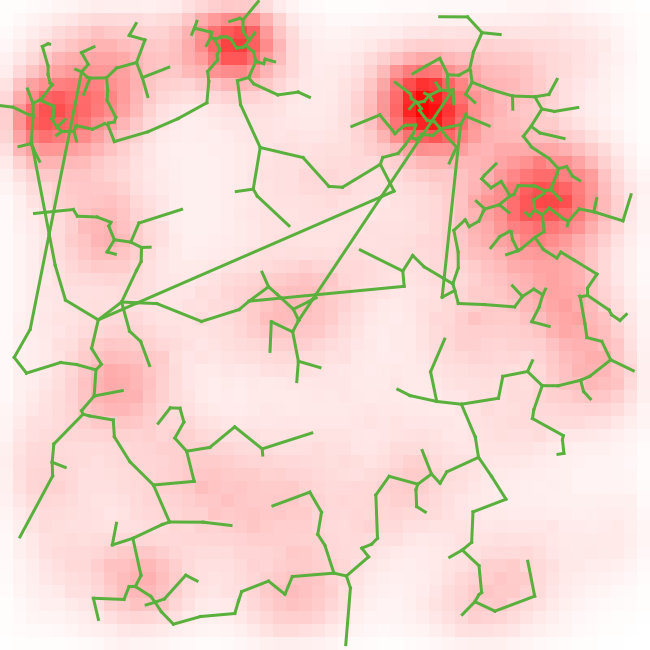
\includegraphics[width=\textwidth]{Figures/Cover/cover} \\ \vspace{0.5cm} % Picture

Présentée par\\
\spacedlowsmallcaps{\myName}\\ % Your name
\bigskip


%\mySubtitle \\ \medskip % Thesis subtitle
%Under the supervision of \myProf and \myOtherProf \\ \medskip
Sous la direction de \myProf et \myOtherProf \\ \medskip
%\myDegree \\
\myDepartment \\  \medskip
%\myFaculty \\  \bigskip
%\myUni \\ \bigskip

\bigskip

\myTime\ -- \myVersion % Time and version

\bigskip

Composition du Jury :

\noun{Arnaud Banos}, Directeur de Recherche, CNRS (Directeur)\\
\noun{Florent Le Néchet}, Maître de Conférence, Université Paris-Est (Directeur)\\

\vfill

\end{center}
\end{addmargin}

\end{titlepage} % Main title page

% Back of the title page

\thispagestyle{empty}

\hfill

\vfill

\noindent\myName: \textit{\myTitle,} \mySubtitle, %\myDegree, 
\textcopyright\ \myTime

% You may wish to do something with the back of the title page, such as including your supervisors, location or time frame of the work. Below is an example of doing so although you may want to tweak it to your liking.

%\bigskip

%\noindent\spacedlowsmallcaps{Supervisors}: \\
%\myProf \\
%\myOtherProf \\ 
%\mySupervisor

%\medskip \\

%\noindent\spacedlowsmallcaps{Location}: \\
%\myLocation

%\medskip \\

%\noindent\spacedlowsmallcaps{Time Frame}: \\
%\myTime
 % Back of the title page

\cleardoublepage% Dedication

\thispagestyle{empty}
\refstepcounter{dummy}

\pdfbookmark[1]{Dedication}{Dedication} % Bookmark name visible in a PDF viewer

\vspace*{3cm}



\bpar{
Our relation to our environment and people change at time scales we generally expect larger. Social relations are neither stationary nor in any kind of equilibrium at any time. They are chaos and complexity, as one's mind. As a witness, we include this preliminary dedication, for comparison purposes with the final version.
}{

}


%\begin{center}
%\emph{Ohana} means family. \\
%Family means nobody gets left behind, or forgotten. \\ \medskip
%--- Lilo \& Stitch    
%\end{center}
%
%\medskip
%
%\begin{center}
%Dedicated to the loving memory of Rudolf Miede. \\ \smallskip
%1939\,--\,2005
%\end{center} % Dedication page

\cleardoublepage% Abstract

%\renewcommand{\abstractname}{Abstract} % Uncomment to change the name of the abstract

\pdfbookmark[1]{Résumé}{Résumé} % Bookmark name visible in a PDF viewer

\begingroup
\let\clearpage\relax
\let\cleardoublepage\relax
\let\cleardoublepage\relax

%\chapter*{Abstract}{Résumé}
\chapter*{Résumé}
%Short summary of the contents\dots a great guide by 
%Kent Beck how to write good abstracts can be found here:  
%\begin{center}
%\url{https://plg.uwaterloo.ca/~migod/research/beckOOPSLA.html}
%\end{center}


La question récurrente de potentiels effets structurants des infrastructures de transports sur les territoires, est l'un des aspects de la problématique plus large des interactions entre réseaux et territoires. Celles-ci sont l'une des facettes de dynamiques territoriales complexes, au sein desquelles territoires et réseaux de transport seraient en co-évolution. L'objectif de cette thèse est de mettre à l'épreuve cette vision des interactions entre réseaux et territoires, autant sur le plan conceptuel qu'empirique, dans le but de l'intégrer au sein de modèles de simulation des systèmes territoriaux. La nature intrinsèquement multi-disciplinaire de la question nous conduit dans un premier temps à une analyse d'épistémologie quantitative, qui permet de dresser une carte du paysage scientifique et une description précise de la structure des différents modèles dans chaque discipline. La définition de la co-évolution et une méthode de caractérisation empirique, basée sur une analyse de correlations spatio-temporelles, est élaborée. Deux pistes complémentaires de modélisation, correspondant à des ontologies et des échelles différentes sont alors explorées. A l'échelle macroscopique, nous développons une famille de modèles dans la lignée des modèles d'interaction au sein des systèmes de villes développés par la Théorie Evolutive des Villes. Leur exploration montre qu'ils capturent effectivement des dynamiques de co-évolution, et leur calibration sur données démographiques pour le système de villes français (1830-1999) quantifie l'évolution des processus d'interaction comme l'effet tunnel ou le rôle de la centralité. A l'échelle mesoscopique, un modèle de morphogenèse capture la co-évolution de la forme urbaine et de la topologie du réseau. Il est calibré sur les indicateurs correspondants pour la forme et la topologie locales calculés pour l'ensemble de l'Europe. De multiples processus d'évolution du réseau (planification coût-bénéfices, rupture de potentiel, auto-organisation) sont montrés complémentaires pour produire l'ensemble des configurations réelles. La calibration est également faite au second ordre, c'est à dire sur les interactions entre indicateurs, pour lequel le modèle reproduit une grande diversité de situations existantes. Ces résultats suggèrent d'une part une construction théorique intégrant Théorie Evolutive Urbaine et Morphogenèse, et ouvrent d'autre part l'exploration d'une nouvelle génération de modèles urbains intégrant les dynamiques co-évolutives dans une perspective multi-échelles.




%-----------------------------------------------

\newpage

\cn{
\chapter*{建模交通网络和地域的共同演变 : 摘要}
}

\cn{运输基础设施对领土体系结构效应存在的问题远未得到解决。% La question de l'existence d'effets structurants des infrastructures de transports sur les systèmes territoriaux est loin d'être résolue. 
这是复杂的地域动态的一个方面,其中领土和交通网络正在共同演变。% C'est l'une des facettes de dynamiques territoriales complexes, au sein desquelles territoires et réseaux de transport sont en co-évolution.
这篇论文的目的是测试网络和地域之间的相互作用。%L'objectif de cette thèse est de mettre à l'épreuve cette vision des interactions entre réseaux et territoires.
它将在概念和经验上做到这一点,目的是将其整合到地域系统的模拟模型中。% Elle le fera autant sur le plan conceptuel que le plan empirique, dans le but de l'intégrer au sein de modèles de simulation des systèmes territoriaux.
我们正在处理的问题本质上是多学科的。% La problématique que nous traitons est intrinsèquement multi-disciplinaire.
出于这个原因,我们首先进行量化的认识论分析。% Pour cette raison, nous procédons dans un premier temps à une analyse d'épistémologie quantitative. 
它可以绘制科学的景观图,并精确地描述每个学科不同模型的结构。% Elle permet de dresser une carte du paysage scientifique et une description précise de la structure des différents modèles dans chaque discipline.
我们制定了一个共同进化的定义,并开发了一个基于时空相关分析的经验表征方法。% Nous élaborons une définition de la co-évolution et élaborons une méthode de caractérisation empirique basée sur une analyse de correlations spatio-temporelles.
探索两个互补的建模轨道。 它们对应于不同的本体和尺度。% Deux pistes complémentaires de modélisation sont explorées. Elles correspondent à des ontologies et des échelles différentes.
在宏观层面上,我们根据城市演变理论发展起来的城市体系内的相互作用模型发展了一个模型家族。% A l'échelle macroscopique, nous développons une famille de modèles dans la lignée des modèles d'interaction au sein des systèmes de villes développés par la Théorie Evolutive des Villes.
他们的探索表明,他们实际上捕捉到共同演化的动力。 他们对法国城市系统(1830-1999)的人口统计数据的校准量化了互动过程的演变。 这些例如是隧道效应或网络中心性的影响。% Leur exploration montre qu'ils capturent effectivement des dynamiques de co-évolution. Leur calibration sur données démographiques pour le système de villes français (1830-1999) quantifie l'évolution de processus d'interaction. Ceux-ci sont par exemple l'effet tunnel ou l'impact de la centralité dans le réseau.
在介观尺度上,形态演化模型捕捉城市形态和网络拓扑的共同演化。% A l'échelle mesoscopique, un modèle d'évolution morphologique capture la co-évolution de la forme urbaine et de la topologie du réseau.
根据整个欧洲计算的局部形态和拓扑结构的相应指标进行校准。% Il est calibré sur les indicateurs correspondants pour la forme et la topologie locales calculés pour l'ensemble de l'Europe.
网络演进的多个过程被考虑到:成本效益计划,潜在的突破,自组织。 它们似乎是互补的,可以产生所有的真实配置。% De multiples processus d'évolution du réseau sont pris en compte : planification coût-bénéfices, rupture de potentiel, auto-organisation. Ils apparaissent complémentaires pour produire l'ensemble des configurations réelles. 
校准也是按照第二顺序进行的,也就是指标之间的相互作用,模型重现了现有情况的多样性。% La calibration est également faite au second ordre, c'est à dire sur les interactions entre indicateurs, pour lequel le modèle reproduit une grande diversité de situations existantes.
这些结果一方面表明了把城市演变理论与形式演变相结合的理论建构。 另一方面,他们开辟了新一代城市模式的探索,这些模型将不得不整合多尺度协同进化动力学。% Ces résultats suggèrent d'une part une construction théorique intégrant Théorie Evolutive Urbaine et évolution de la forme. Ils ouvrent d'autre part l'exploration d'une nouvelle génération de modèles urbains qui devra intègre les dynamiques co-évolutives multi-échelles.
}





%-----------------------------------------------

\newpage

\chapter*{Abstract}











% old abstract

%Territorial systems exhibit complexity at any levels and for most of their aspects. Related disciplines \comment{(Florent) geography, planning, socio, economy}
%generally embrace complex systems science approaches to tackle their understanding and the associated dramatic \comment{(Florent)un peu fort ?}
%social and environmental issues. Choosing a specific angle of lecture of territories, \comment{(Florent)trop vite ds problématique, développer d'abord aspect dynamique}, idem
%it appears, following territorial theories of networks, that real networks play a crucial role in system dynamics, and in particular transportation networks. Taking furthermore a modeling paradigm, we ask to what extent a modeling approach to territorial systems as networked human territories can help disentangling complexly involved processes. We propose to build an associated theory, relying on a vision of human territories as networked, combined with the evolutive urban theory and insights from morphogenesis and co-evolution, that we call a \emph{theory of co-evolutive networked territorial systems}. \comment{(Florent) pas clair, pas forcément nommer}
% It is then embedded into a more general epistemological framework insisting on the notions of emergence and modularity. Quantitative epistemological analysis \comment{(Florent)trop précis}
% confirm the manual literature review and guide research towards co-evolutive models of networks and territories. We search for stylized facts in empirical datasets to also guide model construction. Methodological developments allow to expect information on dynamical processes from static correlations between urban morphology and network shape. The first modeling experiments include a calibrated spatial model of urban growth, giving an insight into theoretical assumption of network necessity. This model is then weakly coupled with a network generation heuristic to explore the space of feasible correlations. It paves the road for both comparison with real correlations and a strongly coupled calibrated model. We also explore novel paradigms such as the role of governance processes in network growth, through a game-theoretic agent-based model. These preliminary results provide the roadmap towards a family of comprehensive operational models of co-evolution between networks and territories that aim to disentangle their circular causalities.
%\comment{(Florent) trop de concepts dans l'abstract, peut pas apporter qqchse à tous}
%\comment{(Florent) commencer par expliquer ce que sont causalités circulaires et pourquoi difficiles à modéliser}
%\comment{(Arnaud) complexly : ?}
%\comment{(Arnaud) théorie des systèmes territoriaux en réseau co-évolutifs ?}





\endgroup			

\vfill % Abstract page



\cleardoublepage
% Abstract

%\renewcommand{\abstractname}{Abstract} % Uncomment to change the name of the abstract

%\pdfbookmark[1]{Reading Notes}{Reading Notes} % Bookmark name visible in a PDF viewer
\pdfbookmark[1]{Notes de Lecture}{Notes de Lecture}

\begingroup
\let\clearpage\relax
\let\cleardoublepage\relax
\let\cleardoublepage\relax

%\chapter*{Reading Notes}{Notes de Lecture}

\chapter*{Notes de Lecture}



Cette thèse devait initialement être rédigée en anglais pour sa version originale. Un premier tiers et la majorité des articles l'ont été, pour être repris et traduits par la suite, afin de répondre à une contrainte administrative d'un autre âge. Elle avait également été conçue comme une ``thèse à articles'', mais les fortes recommandations du CNU ont vite eu vent de cette ambition. Ainsi, la version courante est passée par maintes transformations et ``lissages'', afin de lui donner une forme, un fond et une identité ``classiques''. Nous nous excusons préalablement auprès du lecteur si des écueils de traduction ou d'articulation subsistent et perturbent la fluidité de la lecture.

L'ensemble des figures est produit par l'auteur, sauf la figure~\ref{fig:computation:xkcd} (source xkcd). La grande majorité des figures est \emph{directement} reproductible, c'est à dire pouvant être obtenue par execution des scripts. L'ensemble des codes sources, des modèles à l'interprétation des résultats et à cette propre rédaction, est disponible de manière ouverte avec l'ensemble de son historique atomique (\emph{commits}) sur le dépôt du projet\footnote{à \url{https://github.com/JusteRaimbault/CityNetwork}}. L'ensemble des jeux de données produits dans ce cadre est ouvert, et l'ensemble des données utilisées sont ouvertes ou rendues ouvertes (de manière agrégée correspondant au niveau d'utilisation par les modèles dans le cas d'une base tierce fermée).

Ce mémoire en lui-même a été relu par les lecteurs suivants (ordre alphabétique) : Arnaud Banos (AB), Florent Le Néchet (FL), Clémentine Cottineau (CC), dans l'esprit d'une revue ouverte : en suivant les commits successifs à \url{https://github.com/JusteRaimbault/ThesisMemoire}, l'utilisation de commandes spécifiques permet de retracer l'ensemble du processus de revue.



\endgroup			

\vfill







%\textit{Cette thèse est un voyage, tout d'abord géographique au travers des territoires très divers que nous visiterons tout autour du monde et dans des mondes qui n'existent pas. Un voyage entre des disciplines qui n'ont pas forcément l'habitude de se parler. Un voyage au delà des illusions et des idéaux naïfs sur une recherche qui serait surhumaine, un voyage initiatique dans la médiocrité quotidienne et l'étroitesse d'esprit, particulièrement dans ses relations à l'enseignement. Un trip sous drogues diverses qui aura cherché un sens jusqu'au bout pour comprendre que le sens du sens lui-même n'en avait pas. Une exploration préliminaire effleurant l'immensité des voyages qui nous attendent plus tard.}


 % Uncomment and create a Foreword.tex to include a foreword



\cleardoublepage% Publications - a page listing research articles written using content in the thesis

\pdfbookmark[1]{Publications}{Publications} % Bookmark name visible in a PDF viewer

\chapter*{Publications} % Publications page text

%Some ideas and figures have appeared previously in the following publications:\\

%\noindent Put your publications from the thesis here. The packages \texttt{multibib} or \texttt{bibtopic} etc. can be used to handle multiple different bibliographies in your document.

%\begin{refsection}[ownpubs]
%    \small
%    \nocite{*} % is local to to the enclosing refsection
%    \printbibliography[heading=none]
%\end{refsection}

%\emph{Attention}: This requires a separate run of \texttt{bibtex} for your \texttt{refsection}, \eg, \texttt{ClassicThesis1-blx} for this file. You might also use \texttt{biber} as the backend for \texttt{biblatex}. See also \url{http://tex.stackexchange.com/questions/128196/problem-with-refsection}.

\bpar{
The following works have an highly overlapping content with this thesis:
}{
Les travaux suivants contiennent une grande partie du contenu de cette thèse:
}

% NOTE : on self-plagiarism, be careful to precise when extract from a published paper : 
%  - http://academia.stackexchange.com/questions/12342/self-plagiarism-in-phd-thesis
%  - http://academia.stackexchange.com/questions/2029/can-i-use-the-work-in-my-journal-conference-publications-as-chapters-in-my-disse
%  - http://academia.stackexchange.com/questions/149/what-is-a-sandwich-thesis


\section*{Publications}{Publications}


\noindent Antelope, C., Hubatsch, L., Raimbault, J., and Serna, J. M. (2016). An interdisciplinary approach to morphogenesis. Forthcoming in Proceedings of Santa Fe Institute CSSS 2016.


\bigskip

\noindent Raimbault, J. (2017). A Discrepancy-Based Framework to Compare Robustness Between Multi-attribute Evaluations. In Complex Systems Design \& Management (pp. 141-154). Springer International Publishing. \cite{raimbault2016discrepancy}

\bigskip

\noindent Raimbault, J. (2016). Investigating the Empirical Existence of Static User Equilibrium, \textit{forthcoming in EWGT 2016 proceedings, Transportation Research Procedia.} arxiv:1608.05266 \cite{raimbault2016investigating}


\bigskip


\noindent Raimbault, J. (2016). Generation of Correlated Synthetic Data, forthcoming in \textit{Actes des Journ{\'e}es de Rochebrune 2016.}


\bigskip

\noindent Raimbault, J. (2015). Models Coupling Urban Growth and Transportation Network Growth: An Algorithmic Systematic Review Approach, forthcoming in \textit{ECTQG 2015 proceedings.} arxiv:1605.08888


\section*{Communications}{Communications}

\noindent Towards a Theory of Co-evolutive Networked Territorial Systems: Insights from Transportation Governance Modeling in Pearl River Delta, China, \textit{MEDIUM Seminar : Sustainable Development in Zhuhai, Guangzhou, Dec 2016.}


\bigskip


\noindent Models of growth for system of cities : Back to the simple, \textit{Conference on Complex Systems 2016, Amsterdam, Sep 2016.}



%Raimbault J., Bergeaud A. and Potiron Y. (2016). Investigating Patterns of Technological Innovation. \textit{Conference on Complex Systems 2016, Amsterdam, Sep 2016.}


\bigskip

\noindent For a Cautious Use of Big Data and Computation. \textit{Royal Geographical Society - Annual Conference 2016 - Session : Geocomputation, the Next 20 Years (1), London, Aug 2016.}


\bigskip

\noindent Indirect Bibliometrics by Complex Network Analysis. \textit{20e Anniversaire de Cybergeo, Paris, May 2016.}


\bigskip

\noindent Raimbault, J. \& Serra, H. (2016). Game-based Tools as Media to Transmit Freshwater Ecology Concepts, \textit{poster corner at SETAC 2016 (Nantes, May 2016).}


\bigskip

\noindent Le Néchet, F. \& Raimbault, J. (2015). Modeling the emergence of metropolitan transport authority in a polycentric urban region, \textit{ECTQG 2015, Bari, Sep 2015).}


\bigskip

\noindent Hybrid Modeling of a Bike-Sharing Transportation System, \textit{poster presented at ICCSS 2015, Helsinki, June 2015.}

\bigskip

\noindent Raimbault, J. \& Gonzales, J. (2015). Application de la Morphog{\'e}n{\`e}se de R{\'e}seaux Biologiques {\`a} la Conception Optimale d'Infrastructures de Transport, \textit{poster presented at Rencontres du Labex Dynamite, Paris, May 2015.}


 % Publications from the thesis page

\cleardoublepage% Acknowledgements

%\pdfbookmark[1]{Acknowledgements}{Acknowledgements} % Bookmark name visible in a PDF viewer
\pdfbookmark[1]{Remerciements}{Remerciements}

%\begin{flushright}{\slshape    
%We have seen that computer programming is an art, \\ 
%because it applies accumulated knowledge to the world, \\ 
%because it requires skill and ingenuity, and especially \\
%because it produces objects of beauty.} \\ \medskip
%--- \defcitealias{knuth:1974}{Donald E. Knuth}\citetalias{knuth:1974} \citep{knuth:1974}
%\end{flushright}

%\bigskip

%----------------------------------------------------------------------------------------

\begingroup

\let\clearpage\relax
\let\cleardoublepage\relax
\let\cleardoublepage\relax

%\chapter*{Acknowledgements}
\chapter*{Remerciements}


% \textit{La forme et la fonction se produisent mutuellement de manière complexe. Des remerciements ne feraient pas partie du fond scientifique ? }

% grille

Un certain nombre de résultats obtenus dans cette thèse ont été calculés sur l'organisation virtuelle vo.complex-system.eu de l'European Grid Infrastructure (http://www.egi.eu). Nous remercions l'European Grid Infrastructure et ses National Grid Initiatives (France-Grilles en particulier) pour fournir le support technique et l'infrastructure. \\



% directeurs

% Ma profonde reconnaissance va naturellement en très grande partie à mes directeurs, qui ont rendu cette aventure possible et ont permis sa forme finale, par un pilotage subtil du système complexe que formait mes objets, mes modèles, mes idées. J'ai rencontré pour la première fois Arnaud Banos en octobre 2012 à l'ISC qu'il dirigeait, alors toujours rue Lhomond. C'était dans le cadre d'une supervision des \emph{Open Problems} du PA Systèmes Complexes, et nous nous étions immergés avec mon collègue Jorge dans le monde du multi-échelle, de l'optimisation multi-objectif, des réseaux biologiques auto-organisés (projet dont l'implémentation originale a d'ailleurs été reprise ici).


% Je tiens également à remercier Paul Bourgine et Kashayar Pakdaman











%%%%%%%%%%%
%% Invitation soutenance

% -> positionnement scientifique / impact potentiel

% personnalités scientifiques
% - A. Bonnafous
% - F. Laurent
% - N. Aveline
% - C. Rozenblat
% - L. D'Acci
% - D. Chavalarias
% - F. Varenne
% - F. Pfaender
% - D. Badariotti
% - L. Sanders
% - M. Barthelemy
% - J.P. Marchand
% - F. Durand-Dastès
% - P. Frankhauser


% SFICSS
% - European circ eco crew : Joris, Marius, Mario.
% - Matteo
% - Jelena

% LVMT
% -> annonce interne

% Geocités
% -> annonce interne

% ISC
% -> annonce interne

% EMCSS
% - Kashayar Pakdaman, René Doursat
% - anciens du master cs (via Mme Taki ?)
% - Carantino
% - Jorge

% CSSS2013
% - Claire, Nico


% X
% - Heliou(s), Buisson


% Ponts
% - Camille

% Medium
% - collègues Medium si en Europe
% - Elfie, Medhi

% Coauteurs
% (rq : // diagramme Clem : overlap avec potes etc)
% - Marion, Romain, Clem
% - Solène

% eleves
% ?


% potes
% - Anto, Yo (si en fr), Max, Arnaud
% - SFR
% - Axel
% - Hélène (et parents)
% - Cinzia
% - Solène, Charline


% autres
% - Hervé












\endgroup % Acknowledgements page

\pagestyle{scrheadings} % Show chapter titles as headings

\cleardoublepage% Table of Contents - List of Tables/Figures/Listings and Acronyms

\refstepcounter{dummy}

\pdfbookmark[1]{\contentsname}{tableofcontents} % Bookmark name visible in a PDF viewer

\setcounter{tocdepth}{1} % Depth of sections to include in the table of contents - currently up to subsections

\setcounter{secnumdepth}{2} % Depth of sections to number in the text itself - currently up to subsubsections

\manualmark
\markboth{\spacedlowsmallcaps{\contentsname}}{\spacedlowsmallcaps{\contentsname}}
\tableofcontents 
\automark[section]{chapter}
\renewcommand{\chaptermark}[1]{\markboth{\spacedlowsmallcaps{#1}}{\spacedlowsmallcaps{#1}}}
\renewcommand{\sectionmark}[1]{\markright{\thesection\enspace\spacedlowsmallcaps{#1}}}

\clearpage

\begingroup 
\let\clearpage\relax
\let\cleardoublepage\relax
\let\cleardoublepage\relax

%----------------------------------------------------------------------------------------
%	List of Figures
%----------------------------------------------------------------------------------------

\refstepcounter{dummy}
%\addcontentsline{toc}{chapter}{\listfigurename} % Uncomment if you would like the list of figures to appear in the table of contents
\pdfbookmark[1]{\listfigurename}{lof} % Bookmark name visible in a PDF viewer

\begin{adjustwidth*}{-1cm}{-2cm}

\listoffigures

\end{adjustwidth*}

\vspace{8ex}
%\newpage

%----------------------------------------------------------------------------------------
%	List of Tables
%----------------------------------------------------------------------------------------

\refstepcounter{dummy}
%\addcontentsline{toc}{chapter}{\listtablename} % Uncomment if you would like the list of tables to appear in the table of contents
\pdfbookmark[1]{\listtablename}{lot} % Bookmark name visible in a PDF viewer

%\chapter*{List of Tables}

\begin{adjustwidth*}{-1cm}{-2cm}

\phantomsection

\listoftables

\end{adjustwidth*}
        
\vspace{8ex}
\newpage
    
%----------------------------------------------------------------------------------------
%	List of Listings
%---------------------------------------------------------------------------------------- 

%\refstepcounter{dummy}
%\addcontentsline{toc}{chapter}{\lstlistlistingname} % Uncomment if you would like the list of listings to appear in the table of contents
%\pdfbookmark[1]{\lstlistlistingname}{lol} % Bookmark name visible in a PDF viewer

%\lstlistoflistings 

%\vspace{8ex}
%\newpage
       
%----------------------------------------------------------------------------------------
%	Acronyms
%----------------------------------------------------------------------------------------

%\refstepcounter{dummy}
%\addcontentsline{toc}{chapter}{Acronyms} % Uncomment if you would like the acronyms to appear in the table of contents
%\pdfbookmark[1]{Acronyms}{acronyms} % Bookmark name visible in a PDF viewer

%\markboth{\spacedlowsmallcaps{Acronyms}}{\spacedlowsmallcaps{Acronyms}}

%\chapter*{Acronyms}

%\begin{acronym}[ABM]
%\acro{ABM}{Agent-based Modeling}
%\acro{API}{Application Programming Interface}
%\acro{UML}{Unified Modeling Language}
%\end{acronym}  
             
             

%\begin{acronym}[SOC]
%\acro{ABM}{Self-organized Criticality}
%\end{acronym} 
             
             
             
                   
\endgroup % Contents, list of figures/tables/listings and acronyms

\cleardoublepage

\pagenumbering{arabic} % Arabic page numbering for thesis content (1, 2, 3, etc)
%\setcounter{page}{90} % Uncomment to manually start the page counter at an arbitrary value (for example if you wish to count the pre-content pages in the page count)

\cleardoublepage % Avoids problems with pdfbookmark

%----------------------------------------------------------------------------------------
%	THESIS CONTENT - CHAPTERS
%----------------------------------------------------------------------------------------






%%%%%%%%%%%%%%%%%%%%
%% Organisation and general points



\comment{(Florent) cf receuil articles du Monde sur Grd Paris (numériser)}

\comment{(Florent) HDR Anne ?}


\comment{(Florent) trop peu ancré concrètement dans le champ des interactions transport/ville - enchainement idée ok mais revoir granularité info. Catalogue de situations complexes d'interactions forme urbaine/transport à reproduire.}





%%%%%%%%%%%%%%%%%%%%
% TODO - todo
%
% -- TODO --

% - checker redondances bibliographie, et exactitude des records, publications arxiv, etc. !! biblio des appendices dans la générale ? a voir.
% - inclure éthique de la connaissance de Monod.
% - why not include artwork as appendix. science<->art (// poésies ?)
% - appendix : ecogeo - include results and discussions ; idem conf Medium ?
% - Morphogenesis : * reclarify link between dynamics and form in Thom's theory ; * find time to do quant epistemo ; * on the definition of the system and boundaries : missing part ?
% - somewhere clarification and discussion on definitions of emergence, Bedau etc. ? done on several points.
% - sur multi-scale modeling : who does some and how much ? à ajouter quelque part
% - pour la PDE : voir Villani, mentionner ?
% - effective dimension of urban system : sens ? (comment density) : question assez profonde à méditer - lié info sémantique portugali ? lié représentation minimale ?
% - on density multi-scale dvlpmt : pas clair ce que tu as en tête ici : je ne sais pas si tu auras le temps de creuser cela, mais pour du multi-scalaire, les schémas sont très aidant car c'est vite difficile à visualiser
% - morphogénétiques : est-ce que le mot existe, orthographe pas logique !
% - correlated synthetic data : appendix : inclure regressions
% - revoir discussion correlated synthetic data
% - aller interviewer JP Marchand (Theo Quant) (citation comprendre la co-évolution)
% - make tables uniform and clean
% - recompute indicators with capacity and/or hierarchy when possible with speed limits, to check how they change, and also correlations ? -> speeds pas assez fiables a priori ; fait toujours avec dans tous les cas
% - \cite{2015arXiv150600348A} : Enhanced Gravity Model, how to take better into account heterogeneous network topology, using entropy maximisation combined to gravity model. : a caser quelque part, ressemble sur le coupling, et gravité (sugg. intgib au début)

% - Knowledge framework : 
%    * portugali IRSSN dans la partie theory - conceptualisation.
%    * introduce necessary domains : at least of necessary domains, that we postulate these ones ; there may be an infinity  ?
%    * ajouter des éléments interview Clem.

% - Modelography : 
%    * tenter une classif endogène des modèles : selon les caractéristiques récupérées ? pas forcément pertinent vu taille des données
%    * processus extraction de manière ``synthétique'' : implique des catégories, des choix subjectif. ; idem région géographique : suppose une typologie de classement, niveaux etc. Both out of purpose for now.
%    * idem  pour modèles statistiques : conclusion sens causalité/signif. Travail plus poussé en lui-même. A Faire plus tard.
%

% - interviews : voir où inclure, selon quantité et contenu.

% - partie supplémentaire dans Modélographie : dissection précise des vrais modèles de coévolution ? (pas tant que ça).

% - (Arnaud) (sur le plan) : dans méthodo : ajouter Modèle agents - hors équilibre -> small part in review.

% - StaticCorrelations : 
%    * finir-choisir maps pour la Chine en annexe ; complémentaires celles Europe ?
%    * GWR pour échelle optimale.
%
% - CausalityRegimes : \cite{kasraian2010interaction} à caser dans les études stat ?
%
% - observation flottante : La disposition d'esprit peut être rapprochée de la philosophie -> zen ? pshychédélique ici ?

% - Macro exploration : explorer le Portugali ?

% - Macro application FR : base autoroutes ("data paper" en annexe ? -> penser à faire un vrai data paper avec Florent.)

% - (thematic 1.1.1) \comment{(Florent)pas besoin ni interet de se positionner sur emergence des societes} : si car lié à évolution culturelle, les villes comme étape de celle-ci : dans une perspective plus large (cf projet postdoc), fondamental.

% - (thematic 1.1.1) \comment{(Florent)Une strategie à adopter serait d'abord de decrire de facon basique, avec exemples concrets, la complexité des interactoins réseau/espace/settelements, puis de rappeler CS et proprietes, puis de decrire lesquelles de ces propriétés presentes dans ces interactions, lequelles modèles vont essayer de reproduire et pquoi.} -> le problème, comme le révèle la modelography et la biblio, puis les expériences de modélisation, trop vaste, notion coevol mal définie, peut d'info systématiques. la partie fondations fait partiellement ce travail, seulement après celle-ci on peut avoir une vision un peu plus claire. --  \comment{(Florent) TB mais en parler avant, c'est cela le coeur} (difficulté intrinsèque, réseau qui façonnent territoire)

% - Gaelle Lesteven Metro toulouse - thèse : http://confins.revues.org/7653 ; exemple postdoc ? pas publié a priori.



%% -- DONE --
%
%  X - attention aspect uniformisateur/limite totalitariste vision sci ? -> ok clarifier avec anarchisme et Feyerabend.
%  X - trouver un moyen d'élargir systématiquement toutes les figures ?

%%%%%%%%%%%%%%%%%%%%
% TODO - include notes

% -> notes.md




%%%%%%%%%%%%%%%%%%%%
% TODO - Reading Records
%
%% -- A LIRE -- 

% - lire Morin sur la pensée complexe
% - Moore Nature of Computation
% - (Arnaud) A LIRE : R Brunet, Discontinuités en géographie ; Pierre Dumolard (Espace Différencié) ; Guy DiMeo (L'homme, la société, l'espace)


%% -- A INCLURE --
%



%%%%%%%%%%%%%%%%%%%%
% TODO - Ideas

% - cours : la ville est la combinaison de forces opposées, souvent contradictoire. (cours analyse spatiale). far-from-equilibrium of course.

%  -- URGENT -- (when writing comments on network growth models) : do a sort of list of processes, implied objects, etc. / or a tab , from modeling, theories and CASES STUDIES --


% -  companion site à la Seb ?

% -  a note on open review via git ?



%%%%%%%%%%%%%%%%%%%%
% TODO - Citations
%
% -> potential citations

%  - Le sérieux n'est que la crasse accumulée dans les têtes vides - Roland Topor

%  - Science is an essentially anarchic enterprise - Paul Feyerabend, Against Method

%\headercit{Mais ce n'est pas une question d'{\^a}ge, de chiffres et de stats\\ Moi je te parle surtout de rage, de kif et d'espoir}{Youssoupha}{\textit{, Esperance de Vie}}

% %\headercit{Do or do not. There is no try.}{Yoda}{}

% %\headercit{We need to find Banos' tenth modeling law}{Ren{\'e} Doursat}{}

%%%%
% voie de garage

%  - % The Social Construction of What ?}{Ian Hacking}{\cite{hacking1999social} -> pas vraiment une citation, et pas adapté à grand chose..
 
%\headercit{Your theory is crazy, but not enough to be true.\comment{(Florent) rigolo mais le rapport avec le sujet est discutable}}{Niels Bohr}{}





%%%%%%%%%%%%%%%%%%%%
% TODO - Uncited
%
% -> uncited refs, why.
%
%2017arXiv170108673P -> number of states of HMM : ?
%levy1993t -> Levy theory on territory : need a deeper read and connections.
%pumain2017geography
%batty2017cities
%2017arXiv170107861D
%nicosia2009extending
%10.1371/journal.pone.0170830
%varma2017hpc
%Munafo:2017uq
%railsback2017
%2017arXiv170102973L
%2017arXiv170102383G
%shashok2017can
%miandoabchi2013multi
%farahani2013review
%fujita1982multiple
%bitbol2004autopoiesis
%dollens2014alan
%Chavalarias2016
%2016arXiv161208111S
%2016arXiv161208338T
%friesz1985transportation
%sui2004tobler
%miller2004tobler
%tobler2004first : Tobler giving precisions on the first law of geography
%2016arXiv161205463G
%raimbault2016discrepancy
%raimbault2016investigating
%2016arXiv161102269V
%2015arXiv150402550T
%batty2005agents
%xue2006spatial
%shen2002urban
%xu2005city
%10.1371/journal.pone.0166011
%10.1371/journal.pone.0166004
%2016arXiv161103232L
%hou2011transport
%cao2012accessibility
%huang2016association
%10.1371/journal.pone.0164553
%chan2005location
%tardy2004role
%perret2015roads
%makse1995modelling
%2016arXiv160904636V
%clauset2004finding
%2016arXiv160902000G
%2016arXiv160808839C
%Downey30082016
%osmosis
%xie2009topological
%rozenfeld2008laws
%2016arXiv160805770C
%2016arXiv160806313S
%2016arXiv160806897H
%2015arXiv151207603T
%duranton2007urban
%dimeo2016geographie
%2016arXiv160608103M
%raimbault2016generation
%raimbault2015hybrid
%raimbault2015user
%raimbault2016system
%swerts2013systemes
%swerts2015megacities
%florida2008rise
%hall1982great
%2016arXiv160805266R
%aveline2016medium
%lenechet:halshs-01272236
%2016arXiv160804472J
%ioannidis2005most
%2016arXiv160803608M
%batty2007creative
%chen2012wider
%hall1997modelling
%knowles2016sir
%reid2016decision
%carreira2000mode
%yu2012solving
%wang2015resilience
%masucci2014exploring
%fessel2012physarum
%gaughan2016spatiotemporal
%raimbault2016simpopsan
%10.1371/journal.pone.0160471
%10.1371/journal.pone.0159496
%pan2003croissance
%2016arXiv160708472M
%lyu2016developing
%emangard2009transports
%e18060197
%ishiguro1997bootstrapping
%Woodhouse19072016
%10.1371/journal.pone.0158826
%10.1371/journal.pcbi.1004947
%2016arXiv160703186A
%10.1371/journal.pone.0157261
%saichev2009theory
%karrer2011stochastic
%gastner2006shape
%10.1371/journal.pone.0157728
%2015arXiv150607608T
%2016arXiv160601959F
%sornette1997convergent
%solomon1996spontaneous
%gabaix2003theory
%newling1966urban
%bretagnolle2000long
%pumain2006villes
%okabe1987theoretical
%dellaposta2016endogenous
%Squartini:2013fk
%Takeuchi20153109
%2016arXiv160501949B
%klimek2012empirical
%10.1371/journal.pone.0154839
%2016arXiv160408816Z
%2016arXiv160407876G
%jiang2007topological
%akaike1998information
%heiss2008likelihood
%2005physics..12106P
%hall1990methodology
%burnham2004multimodel
%manning2014stanford
%thom1974stabilite
%benguigui1991suburban
%durand1990notion
%batty1991generating
%dauphine1995chaos
%dupuy:halshs-00438867
%damm1980response
%coffman1998railroad
%knight1977evidence
%goldberg1972evaluation
%alcaly1976transportation
%aveline2003ville
%2016arXiv160402872L
%2016arXiv160400758D
%2016arXiv160404155A
%2016arXiv160403904B
%2015arXiv151104268L
%echenique2012growing
%Brunton12042016
%banos2011christaller
%10.1371/journal.pone.0152686
%dupuy1993geographie
%newman1996land
%kenworthy2002transport
%tirnakli2015standard
%benettin1980lyapunov
%hijmans2015geographic
%10.1371/journal.pone.0151676
%offner2000territorial
%bourgine2010morphogenesis
%Fujita199693
%lenormand2015comparing
%soler2014calculating
%gallotti2015transportation
%krugman1998space
%lenormand2012generating
%decraene2013emergence
%varenne2008epistemologie
%derrible2010complexity
%10.1371/journal.pone.0150932
%10.1371/journal.pone.0148660
%le2015modeling
%mehaffy2007notes
%cuyala2013diffusion
%ciotti2015homophily
%el2006access
%2015arXiv151003797G
%2016arXiv160208451P
%choi2014patent
%shibata2008detecting
%zembri2010new
%2015arXiv150901940M
%schmid1994probabilistic
%noruzi2005google
%bohannon2014scientific
%2015arXiv150601280B
%2016arXiv160106075O
%10.1371/journal.pone.0147913
%barthelemy2015time
%raffestin1982remarques
%Gao:2016ty
%fujita1996economics
%2016arXiv160203774H
%blondel2008fast
%min2011real
%schultz2014random
%jedwab2013transportation
%offner2002x
%bitner2009complex
%raimbault2015models
%2015arXiv151205659M
%achlioptas2009explosive
%10.1371/journal.pone.0146491
%2015arXiv151207715C
%2015arXiv151205259R
%2015arXiv151200946S
%2015arXiv151201423W
%di1998espace
%2015arXiv151105468E
%2014arXiv1403.3005S
%Brummitt20150712
%beckman1996creating
%simini2012universal
%masucci2013gravity
%witten1981diffusion
%kuhnert2006scaling
%aghion2002schumpeterian
%andersson2002urban
%frankhauser1998fractal
%2015arXiv151006326H
%Sinatra:2015yu
%su2008effect
%fraedrich1986estimating
%chen2009spatial
%2015arXiv150909055P
%Perret:2015fk
%2015arXiv150907599C
%2015arXiv150803542B
%pumain2006hierarchy
%vattay2015quantum
%2014arXiv1403.7686B
%2015arXiv150904486M
%2015arXiv150903678R
%2015arXiv150905183R
%2015arXiv150905590H
%2015arXiv150904558J
%Pohlert:2015fk
%cheng2004notes
%cristelli2012there
%fox2005revisiting
%newman2005power
%clauset2009power
%kyriakidou2011applying
%bretagnolle:halshs-00159894
%sanders2006artificial
%courbaud2015applying
%2015arXiv150707878C
%10.1371/journal.pone.0133780
%gilli2005bassin
%servais2004polycentrisme
%leveque:halshs-00280396
%urbanek2011emdist
%wikle1999dimension
%galka2004solution
%vitanov2015test
%hens2015extreme
%2015arXiv150507372L
%pan2013urban
%tretyakov2011fast
%pumain2004urban
%Capozza1990187
%thevenin2013mapping
%schwartz2011spatial
%roth2012long
%10.1371/journal.pone.0029721
%Ye2014200
%donaldson2010railroads
%lucas1998mechanics
%moretti2004human
%banos2012network
%gauvin2009phase
%chen2010characterizing
%kang2012intra
%Karatzoglou:2004uq
%R-Core-Team:2015fk
%anderson1991turning
%underhill1990soviet
%baklanov2015projects
%perret2010multi
%crucitti2006centrality
%frankhauser2008fractal
%pumain1998urban
%Schwarz201029
%hebert2011structural
%batty2006hierarchy
%lugovoy2007analysis
%dorogovtsev2000structure
%pumain2002role : epistemology on TQG
%Mandelbrot1961198
%Mandelbrot195990
%bailey1999funk
%roopkumar2006generalized
%pumain2015multilevel
%reuillon2015
%10.1371/journal.pcbi.1004101
%anas1998urban
%ribeiro2010game
%Roumboutsos2008209
%le2010approche
%ordeshook1986game
%lenechet:halshs-00674059
%lenechet2012
%keitt2011rgdal
%baddeley2004spatstat
%gallego2010population
%hirtzel:tel-01121665
%martin2004generating
%abadie2011synth
%coulombel:tel-00601262
%strano2012elementary
%networkQgis
%mills2000thematic
%fujita2004new
%cookbookForR
%leurent2012disaggregate
%fields1999city
%dori2002object
%zeigler1989devs
%louail:tel-00584495
%goldspink2000modelling
%Liu201326
%lechner2006procedural
%parish2001procedural
%beauguitte2014r
%andersson2003urban
%brown2005spatial
%Magliocca2011183
%Ettema20111
%phan2010agent
%clarke1998loose
%He2006323
%kocabas2006coupling
%Kunz2000597
%zanette1997role
%clarke2007decade
%achibetmorphogenese
%rui2013urban
%lodin2011road
%porta2006network
%andersson2006complex
%eboli2012exploring
%duranton2012urban
%horner2012analyzing
%2013PhRvL.111s8702L
%antoni:hal-00914269
%berroir2005contribution
%guerois2002commune
%hall2006polycentric
%offner:halshs-00438903
%portugali2012complexity
%
%

% X biernacki2000assessing -> empirical likelihood (paper interactionGibrat)
% X bon2017novel -> SJS
% X bettencourt2007growth : Bettencourt scaling theory of cities
% X bourgine2010morphogenesis : in morphogenesis
% X loo1999development : planning transportation in DPR
% X favaro2007croissance : thèse JM Favaro
% X paulus2004coevolution : specialisation of urban areas











%----------------------------------------------------------------------------------------



%%%%%%%%%%%%%%%%%%%%%%%%%%%%%
% Introduction
%
\ctparttext{}
%
\part*{Introduction}
%



%%%%%%%%%%%%%%%%
%%  Introduction
%%%%%%%%%%%%%%%%


%% Contents
%
%    - General considerations on Complex Systems, positioning etc (thesis in cs science etc)
%    - Thematic introduction, geographical introduction of the subject.
%
%   - precisions on v1 memoire : foreword ?
%
%    - reading precisions : organisation, interdependances etc 
%
%   - reflexive aspect : here ?  


%\chapter*{Introduction}{Introduction}
\chapter*{Introduction}


% to have header for non-numbered introduction
\markboth{Introduction}{Introduction}


% -- citations on hold --
%\headercit{\bpar{It's when you shuffle the anthill that you get a touch of all its complexity.}{C'est quand on donne un coup de pied dans la fourmilière qu'on se rend compte de toute sa complexité.\comment[AB]{je persiste a dire que c'est oas une tres bonne idee !}\comment[FL]{Incipit de son directeur de these est maladroit}}
%}{Arnaud Banos}{}



\bigskip




%\bpar{
%``In consequence of a technical issue, traffic is interrupted on the line B of RER, for an unknown duration. More information will be given as soon as available''. There is a high probability that someone having lived or spent some time in the metropolitan region of Paris has already heard this frightening announce and endured the difficult consequences the rest of his day. But he might not be aware of the ramifications of causal cascades induced by this not-so-rare event. Territorial Systems, whatever the layers considered in their definitions, will always be extremely complex and interrelations at numerous temporal and spatial scales participate in the emergent behaviors observed at any levels of the system. Martin is a student who daily commutes from Paris to Palaiseau and will miss today a crucial exam, what will have a profound impact on his professional life : implications at a long time scale, small spatial scale and agent granularity. Yuangsi is connecting Orly and Roissy Airports, in his trip from London to Beijing, will miss his plane and his sister's wedding : large spatial scale, short time scale, agent granularity. A collective petition emerges from users, leading to new social organizational patterns and reaction from transportation authority that results in efforts to increase levels of service : mesoscopic temporal and spatial scale, swarm of agents granularity.
%}{
%``En conséquence d'un problème technique, le trafic est interrompu sur la ligne B du RER pour une durée indéterminée. Plus d'information seront fournies dès que possible''. Il y a des fortes chances pour que quiconque ayant vécu ou passé un peu de temps en région parisienne ait déjà entendu cette annonce glaçante et en ait subi les conséquences pour le reste de la journée. Mais il ne se doute sûrement pas des ramifications des cascades causales induites par cet évènement presque banal. Les systèmes territoriaux, quelles que soient les aspects considérés pour leur définition, ont une complexité croissante lorsqu'on augmente leur nombre, les interrelations à de nombreuses échelles spatiales et temporelles participant à la production des comportements émergents observés à tout niveau du système. Martin est un étudiant qui fait l'aller-retour journalier entre Paris et Palaiseau and manquera un examen crucial, ce qui aura un impact profond sur sa vie professionnelle : implications à une longue échelle de temps, une petite échelle spatiale et à la granularité de l'agent. Yuangxi était en train de relier les aéroports d'Orly et Roissy dans son voyage de Londres à Pékin et va manquer son avion ainsi que le mariage de sa soeur : grande échelle spatiale, courte échelle temporelle, granularité de l'agent. Une pétition collective émerge des voyageurs, conduisant à la création d'une organisation qui mettra la pression sur les autorités pour qu'elles augmentent le niveau de service : échelle temporelle et spatiales mesoscopique, granularité de l'aggregation d'agents.
%\comment[FL]{encore une fois : l'exemple mobilite quotidienne pour commencer me semble mal choisi}
%}


\bpar{}{

}



\bpar{
Looking for causes of the event will also lead to intricate processes at various scales, none of which seems to be a better explication than others : historical railway network in Parisian region shaped further extensions and RER B followed the former \textit{Ligne de Sceaux}, \noun{Delouvrier}'s schema for regional development, and its subsequent partial execution, are elements of explanation of structural weaknesses of Parisian public transportation network~\citep{gleyze2005vulnerabilite}; commuting patterns consequent to territorial organisation induce an overload of particular lines and thus a necessary increase in exploitation incidents. The list could be developed much longer and each approach related to an already mature scientific body of knowledge in different disciplines such as geography, urban economics, transportation. This amusing anecdote is enough to give a touch of the complexity of territorial systems. Our aim here is to dive into this complexity, and in particular to give an original insight into the study of relations between networks and territories. The choice of this reading position will be largely discussed in a further thematic part. Let for now concentrate on the originality of the point of view that we will take.
}{
La recherche de cause possible à l'incident conduira à des processus intriqués à diverses échelles, parmi lesquels aucun ne semble être une meilleure explication ; le développement historique du réseau ferroviaire en région parisienne a conditionné les évolutions futures et le RER B a suivi l'ancienne Ligne de Sceaux, le plan de \noun{Delouvrier} pour le développement régional et son execution partielle, sont également des éléments d'explication de la structure du réseau parisien de transports en commun qui conditionne la perturbation~\cite{gleyze2005vulnerabilite} ; les motifs pendulaires dus à l'organisation territoriale induisent une surcharge de certaines ligne et ainsi nécessairement une augmentation des incidents d'exploitation. La liste pourrait être ainsi continuée un certain temps, chaque approche apportant sa vision mature correspondant à un corpus de connaissances scientifiques dans des disciplines diverses comme la géographie, l'économie urbaine, les transports. Cette anecdote quotidienne est suffisante pour faire ressentir la complexité des systèmes territoriaux. Notre but ici est de se plonger dans cette complexité, et en particulier donner un point de vue original sur l'étude des relations entre réseaux de transport et territoires. Le choix de cette position sera largement discuté dans une partie thématique, nous nous concentrons à présent sur l'originalité du point de vue que nous allons prendre.
}





\section*{On General Positioning}{De la position générale}


\bpar{
\emph{The ambition of this thesis is to have no ambition.} Such an introduction, although seeming rash, contains at all levels the implicit logics behind our research process. At the first degree, we try as much as possible to take a exploratory and constructive approach, as much on theoretical and methodological domains than thematic domain, but also proto-methodological (tools applying the method) : if unidimensional or integrated ambitions should emerge, they would be conditioned to the arbitrary choice of a time sampling among the continuity of the dynamic that structures any research project. In the structural sense, the self-reference that underlines an apparent contradiction points out the centra aspect of reflexivity in our constructive approach, as much in the sense of the recursion of theoretical apparels, than for application of tools and methods developed to the work itself, or in the sense of the co-construction of the different approaches and of the different thematic axis. The processus of knowledge production can this way be read as a metaphor of studied processes. Finally, from a point of view closer to interpretation, it suggests the intention of a delicate position linking a political positioning which necessity is intrinsic to humanities (for example here against the technocratic application of models, or for the development of tools for an Open Science) with a rigor of objectivity coming more from other fields used, position that impose an increased prudence.
}
{
\emph{L'ambition de cette thèse est de ne pas avoir d'ambition.}
 Cette entrée en matière, rude en apparence, contient à différents niveaux les logiques sous-jacentes à notre processus de recherche. Au sens propre, nous nous plaçons tant que possible dans une démarche constructive et exploratoire, autant sur les plans théoriques et méthodologiques que thématique, mais encore proto-méthodologique (outils appliquant la méthode) : si des ambitions unidimensionnelles ou intégrées devaient émerger, elles seraient conditionnées par l'arbitraire choix d'un échantillon temporel parmi la continuité de la dynamique qui structure tout projet de recherche. Au sens structurel, l'auto-référence qui soulève une contradiction apparente met en exergue l'aspect central de la réflexivité dans notre démarche constructive, autant au sens de la récursivité des appareils théoriques, de celui de l'application des outils et méthodes développés au travail lui-même ou que de celui de la co-construction des différentes approches et des différents axes thématiques. Le processus de production de connaissance pourra ainsi être lu comme une métaphore des processus étudiés. Enfin, sur un plan plus enclin à l'interprétation, cela suggérera la volonté d'une position délicate liant une conscience politique dont la nécessité est intrinsèque aux sciences humaines (par exemple ici contre l'application technocratique des modèles, ou pour le développement d'outils luttant pour une science ouverte) à une rigueur d'objectivité plus propre aux autres champs abordés, position forçant à une prudence accrue.
}

%\comment[AB]{Déclaration discutable : si j’ai bien compris l’argumentaire, ton absence d’ambition tient 1) à l’absence de quête d’universalité (dépendance au contexte) et 2) à la dimension politique inhérente à ton objet. Je te ferais dire que 1) l’absence d’universalité n’est pas une tare (c’est même la norme en SHS) et 2) la dissociation science/politique ne tient plus la route depuis bien longtemps et ne concerne qu’un micro domaine des sciences les plus abstraites et théoriques (maths fondamentales, physique théorique peut-être,…what else ?)}[rq : logique proche de Morin - but contenu dans moyen ? - endogene.]



\section*{Scientific Context : Complexity Has Come of Age}{Contexte Scientifique : Paradigmes de la Complexité}


% \footnote{pour lesquels il n'existe pas de définition unifiée mais dont les champs d'application couvrent une étendue allant des neurosciences à la finance quantitative, en passant par exemple par la sociologie quantitative, la géographie quantitative, la biologie intégrative, etc.~\cite{newman2011complex}, et pour l'étude desquels diverses approches complémentaires peuvent être appliquées, comme les Systèmes Dynamiques, la Modélisation Basée Agent, la Théorie des Matrices Aléatoires}


\bpar{
To better introduce our subject, it is necessary to make the reader aware of the particular scientific context we are working in. It is necessary both to understand the general epistemology underlying research questions, and to be aware of the variety of methods and tools used. Contemporaneous science is progressively taking the shift of complexity in many fields.
That also implies an epistemological revolution to abandon strict reductionism that failed in most of its synthesis attempts~\cite{anderson1972more}. Arthur recently recalled~\cite{arthur2015complexity} that a mutation of methods and paradigms was also at stake by the increasing role of computational approaches replacing purely analytical techniques generally self-limited in their modeling and resolution scope. Capturing \emph{emergent properties} in models of complex systems is one of the ways to understand the essence of these new approaches.
}{
Pour une meilleure introduction du sujet, il est nécessaire d'insister sur le cadre scientifique dans lequel nous nous positionnons. Ce contexte est crucial à la fois pour comprendre les concepts épistémologiques implicites dans nos questions de recherche, et aussi pour être conscient de la variété de méthodes et outils utilisés. La science contemporaine prend progressivement le tournant de la complexité dans de nombreux champs que nous illustrerons par la suite, ce qui implique une mutation épistémologique pour abandonner le réductionnisme\footnote{De manière schématique, le réductionnisme consiste en la position épistémologique que les systèmes sont entièrement compréhensibles à partir des éléments fondamentaux les constituant et des lois régissant leur évolution. Les niveaux supérieurs n'ont ni autonomie ni pouvoirs causaux irréductibles.} strict qui a échoué dans la majorité de ses tentatives de synthèse~\cite{anderson1972more}. Arthur a rappelé récemment~\cite{arthur2015complexity} qu'une mutation des méthodes et paradigmes en était également un enjeu, de par la place grandissante prise par les approches computationnelles qui remplacent les résolutions purement analytiques généralement limitées en possibilités de modélisation et de résolution. La capture des \emph{propriétés émergentes} par des modèles de systèmes complexes est une des façons d'interpréter la philosophie de ces approaches.
}



\bpar{
These considerations are well known in Social Science (both quantitative and qualitative), in which the complexity of studied agents and systems is the justification of their existence : if humans were particles a whole branch of fields may have never emerged as thermodynamics would have solved most of social issues. \footnote{even if it would probably not have been the case as classical physics also failed in their attempts to include irreversibility and evolutions of Complex Adaptive Systems as Prigogine points out in \cite{prigogine1997end}} 
They are however less known nor accepted in more ``hard'' sciences such as physics : Laughlin develops in~\cite{laughlin2006different} a view of the discipline 
 at least as at a ``frontier of knowledge'' then other fields appearing as less mature. Most of knowledge is of classical nature although a majority of structures and systems would be \emph{self-organized}, what means that the single microscopic laws are not enough to determine macroscopic properties unless system evolution is simulated (more precisely this property can be taken as a definition of emergence on which we will come back further, and self-organization is intrinsically emergent). It corresponds to the first nightmare of Laplace's Deamon developed in~\cite{deffuant2015visions}.
}{
Ces considérations sont bien connues des Sciences Humaines et Sociales (qualitatives et quantitatives) pour lesquelles la complexité des agents et systèmes étudiés est une des justifications de leur existence : si les humains étaient effectivement des particules, on pourrait s'attendre à ce que la majorité des disciplines les prenant comme objet d'étude n'aient jamais émergé puisque la thermodynamique aurait alors résolu la majorité des problèmes sociaux\footnote{Bien que cette affirmation soit elle-même discutable, les sciences physiques classiques ayant également échoué à prendre en compte l'irréversibilité et l'évolution de Systèmes Complexes Adaptatifs comme le souligne~\cite{prigogine1997end}.}. Elles sont au contraire moins connues et acceptées en sciences ``dures'' comme la physique : \cite{laughlin2006different} développe une vision de la physique à la même position de ``frontière des connaissances'' que d'autre champs plus récents qui pourrait sembler en être encore à leur genèse. La plupart des connaissances actuelles concernent des structures classiques simples, alors qu'un grand nombre de systèmes présentent des propriétés \emph{d'auto-organisation}, au sens où les lois microscopiques ne sont pas suffisantes pour inférer les propriétés macroscopiques du système à moins que son évolution ne soit entièrement simulée (plus précisément cette vision peut être prise comme une définition de l'émergence sur laquelle nous reviendrons par la suite, or des propriétés auto-organisées sont par nature émergentes). Cela correspond au premier cauchemar du Démon de Laplace développé dans~\cite{deffuant2015visions}. 
} 


%-------------------------------------------------



\bpar{
As an informal mix of epistemological positions, methods, and fields of applications, \emph{Complexity Science} relies on typical paradigms such as the centrality of emergence and self-organization in most of phenomena of the real world, which make it lie on a frontier of knowledge closer of us than we can think (Laughlin, op.cit. ). Such concepts are indeed not new, as they were already enlighten by Anderson~\cite{anderson1972more}. Even cybernetics can be related to complexity by seing it as a bridge between technology and cognitive science~\cite{wiener1948cybernetics}.
}{
A la croisée de positionnements épistémologiques, de méthodes et de champs d'application, les \emph{Sciences de la complexité} se concentrent sur l'importance de l'émergence et de l'auto-organisation dans la plupart des phénomènes réel, ce qui les place plus proche de la frontière des connaissances que ce que l'on peut penser pour des disciplines classiques (\noun{Laughlin}, op. cit.). Ces concepts ne sont pas récents et avaient déjà été mis en valeur par~\cite{anderson1972more}. On peut aussi interpréter la Cybernétique comme un précurseur des Sciences de la Complexité en la lisant comme un pont entre technologie et sciences cognitives~\cite{wiener1948cybernetics}, et surtout en développant les notions de retroaction et de contrôle.
}

\bpar{
Later, synergetics~\cite{haken1980synergetics} paved the way for a theoretical approach of collective phenomena in physics. Reasons for the recent growth of works claiming a CS approach may be various. The explosion of computing power is surely one because of the central role of numerical simulations~\cite{varenne2010simulations}. They could also be the related epistemological progresses : apparition of the notion of perspectivism~\cite{giere2010scientific}, finer reflexions around the notion of model~\cite{varenne2013modeliser}\footnote{In that frame scientific and epistemological progress can not be dissociated and can be seen as coevolving}. The theoretical and empirical potentialities of such approaches play surely a role in their success\footnote{
Although the adoption of new scientific practices may be strongly biased by imitation and lack of originality~\cite{dirk1999measure}, or more ambivalent, by marketing strategies as the fight for funds is becoming a huge obstacle for research~\cite{bollen2014funding}.}, as confirmed in various domains of application (see~\cite{newman2011complex} for a general survey), as for example Network Science~\cite{barabasi2002linked} ; Neuroscience~\cite{koch1999complexity}; Social Sciences ; Geography~\cite{manson2001simplifying}\cite{pumain1997pour} ; Finance with the rising importance of econophysics~\cite{stanley1999econophysics} ; Ecology~\cite{grimm2005pattern}. The Complex Systems Roadmap~\cite{2009arXiv0907.2221B} proposed a double lecture of studies on Complex Systems : an horizontal approach connecting fields of study with transversal questions on theoretical foundations of complexity and empirical common stylized facts, and a vertical conceptions of disciplines, with the aim to construct integrated disciplines and corresponding multi-scale heterogeneous models. Interdisciplinarity is thus central in our scientific background.
}{
Plus tard, la Synergétique~\cite{haken1980synergetics} a posé les bases d'approches théoriques des phénomènes collectifs en physique. Les causes possibles de la croissance récente du nombre de travaux se réclamant d'approches complexes sont nombreuses. L'explosion de la puissance de calcul en est certainement une vu le rôle central que jouent les simulations numériques~\cite{varenne2010simulations}. Elles peuvent aussi être à chercher auprès de progrès en épistémologie : introduction de la notion de perspectivisme~\cite{giere2010scientific}, reflexions plus fine autour de la nature des modèles~\cite{varenne2013modeliser}\footnote{Dans ce cadre, les progrès scientifiques et épistémologiques ne peuvent pas être dissociés et peuvent être vus comme étant en co-évolution, au sens d'une forte interdépendance et d'une adaptation mutuelle.}. Les potentialités théoriques et empiriques de telles approchent jouent nécessairement un rôle dans leur succès\footnote{Même si l'adoption de nouvelles pratiques scientifiques peut par ailleurs être biaisé par l'imitation et le manque d'originalité~\cite{dirk1999measure}, ou de façon plus ambivalente, par des stratégies de positionnement indépendante des stratégies de connaissance, puisque le combat pour les fonds est un obstacle croissant à une recherche saine~\cite{bollen2014funding}.}, comme le confirme les domaines très variés d'application (voir~\cite{newman2011complex} pour une revue très générale), comme par exemple la Science de Réseaux~\cite{barabasi2002linked}; les Neurosciences~\cite{koch1999complexity}; les Sciences Humaines et Sociales,  dont la Géographie~\cite{manson2001simplifying}\cite{pumain1997pour}; la Finance avec les approches écononophysiques~\cite{stanley1999econophysics}; l'Ecologie~\cite{grimm2005pattern}. La Feuille de Route des Systèmes Complexes~\cite{2009arXiv0907.2221B} propose une double lecture des travaux en Complexité: une approche horizontale faisant la connexion entre champs d'étude par des questions transversales sur les fondations théoriques de la complexité et des faits stylisés empiriques communs, et une approche verticale, dans le but de construire des disciplines intégrées et les modèles multi-scalaires hétérogènes correspondants. L'interdisciplinarité est ainsi cruciale pour notre contexte scientifique.

}


\section*{Interdisciplinarity}{Interdisciplinarité}



\bpar{
We must further insist on the role of interdisciplinarity in the positions taken here. This is not a thesis in Geography nor in Complex Adaptive Systems Modeling,
 but in \emph{Complex Systems Science} that we claim as a proper discipline following \noun{Paul Bourgine}.
  It will naturally be seen with defiance by scholars of various concerned disciplines, as recent examples of misunderstandings and conflicts have illustrated~\cite{dupuy2015sciences}.
}{
Il est important d'insister sur le rôle de l'interdisciplinarité dans la position de recherche prise ici. Il s'agit autant d'un travail en Géographie Théorique et Quantitative qu'en Modélisation de Systèmes Complexes, étant finalement les deux à la fois selon le point de vue que prendra le lecteur. En ce sens, nous le réclamons de la \emph{Science des Systèmes Complexes} que nous tenterons de positionner comme discipline propre à travers cette implémentation précise\footnote{Un niveau de lecture abstrait du travail dans son ensemble apportera des informations sur la production de connaissance elle-même, comme nous le développerons en~\ref{sec:knowledgeframework}.}. Ce n'est pas sans risques d'être lu avec méfiance voir défiance par les tenants des disciplines classiques, comme des exemples récents de malentendus ou conflits ont récemment illustré~\cite{dupuy2015sciences}. Il faut se rappeler l'importance de la spirale vertueuse de \noun{Banos} entre disciplinarité et interdisciplinarité~\cite{banos2013pour}. Celle-ci doit nécessairement impliquer différents agents scientifiques, et il est compliqué pour un agent de se positionner dans les deux branches ; notre fond scientifique devra nous permettre de ne pas de nous positionner uniquement dans la \emph{disciplinarité géographique} (même si celle-ci sera simultanément une composante cruciale) mais bien aussi dans celle des Systèmes Complexes (qui est interdisciplinaire, voir~\ref{sec:epistemology} pour contourner la contradiction apparente), et notre sensibilité scientifique et épistémologique nous pousse à faire de même.
}

% rq : point de vue = grille de lecture
% \comment[AB]{je trouve que tu abandonnes bien vite la partie. Pourquoi renoncer dès le début alors que tu pourrais laisser la liberté à celui/celle qui te lit de décider si c’est AUSSI de la géo ou non ?}

\bpar{
The positioning of \noun{Batty} proposing \textit{A new Science of Cities}~\cite{batty2013new} (that he subtly presents as \textit{The} new science of cities) is directed towards an integration of disciplines and methods into a science defined by its object of study, cities.
Its theoretical and epistemological weaknesses (no theoretical constructions of studied geographical objects on the one hand, approximative contextualization of complexity) combined with an overall impression of \emph{pot-pourri} of forgotten works
 (space syntax, land-use models), unfortunately avoid us to use it as we will use geographical theories (e.g. evolutive urban theory) in an appropriated epistemological complexity context. Yet our reading of this work may be the result of a misunderstanding due to different cultural backgrounds.
}
{
Le positionnement de \noun{Batty} lorsqu'il propose \textit{Une Nouvelle Science des Villes}~\cite{batty2013new} %(qu'il présente avec humour comme \textit{La} nouvelle science des villes)
, se présente comme une intégration des disciplines et méthodes vers une science définie par son objet d'étude, les villes.
%Its theoretical and epistemological weaknesses (no theoretical constructions of studied geographical objects on the one hand, approximative contextualization of complexity) combined with an overall impression of \emph{pot-pourri} of forgotten works (space syntax, land-use models), unfortunately avoid us to use it as we will use geographical theories (e.g. evolutive urban theory) in an appropriated epistemological complexity context.  Yet our reading of this work may be the result of a misunderstanding due to different cultural backgrounds. \comment[Arnaud]{j'espère que tu abuses ? :) !! Argument d'autorité}[yes, changer positionnement complètement malvenu] \comment[Florent]{attention arguments autorité ; insister sur difficulté à intégrer paradigmes plutot que juger précédents}[idem]
}




\bpar{
The scientific evolution of complexity that some see as a revolution~\cite{colander2003complexity}, or even as \emph{a new kind of science}~\cite{wolfram2002new}, could indeed face intrinsic difficulties due to behaviors and a-priori of researchers as human beings.
 More precisely, the need of interdisciplinarity that makes the strength of Complexity Science may be one of its greatest weaknesses, since the highly partitioned structure of science organization has sometimes negative impacts on works involving different disciplines. We do not tackle the issue of over-publication, competition, indexes, which is more linked to a question of open science and its ethics, also of high importance but of an other nature. That barrier we are dealing with and we might struggle to triumph of, is the impact of certains \emph{cultural disciplinary differences} and out-coming conflicts on views and approaches. 
The drama of scientific misunderstandings is that they can indeed annihilate progresses by interpreting as a falsification some work that answers to a totally different question. The example of a recent work on top-income inequalities given in~\cite{aghion2015innovation}, which conclusions are presented as opposed from the one obtained by Piketty~\cite{piketty2013capital}, follows such a scheme. Whereas Piketty focused on constructing long-time clean databases for income data and showed empirically a recent acceleration of income inequalities, his simple model aiming to link this stylized fact with the accumulation of capital has been criticized as oversimplified. On the other hand, Bergeaud \textit{et al.} prove by a model of innovation economics that \emph{under certain assumptions} income gaps may be beneficial to innovation and consequently a general utility. Thus diverging conclusions about the role of personal capitals in the economy.
But diverging \emph{views} or \emph{interpretations} does not mean a scientific incompatibility, and one could imagine try to gather both approaches in an unified framework and model, yielding possibly similar or different interpretations. This integrated approach has chances to contain more information (depending on how coupling is done) and to be a further advance in Science. In an other but similar vein, \cite{2017arXiv170105627H} reanalyses biological data from a 1943 experiment that claimed to rule out Lamarckian over Darwinian evolution processes, and show that the conclusion are wrong in the current Data analysis (enormous advances in theoretical and processing techniques) and scientific context (with numerous other proofs today of Darwinian processes) : this is a good example of a context-misunderstanding and how conclusions strongly depend on both technical and thematic frameworks. We shall now briefly develop other examples to give an overview how conflicts between disciplines can be damaging.
}{
L'évolution scientifique des sciences de la complexité, qui est vue par certains comme une révolution~\cite{colander2003complexity}, ou même comme \emph{un nouveau type de science}~\cite{wolfram2002new}, pourrait affronter des difficultés intrinsèques dues aux comportements et a-priori des chercheurs en tant qu'être humains. Plus précisément, le besoin d'interdisciplinarité qui fait la force des Sciences de la Complexité pourrait devenir une de ses grandes faiblesses, puisque la structure fortement en silo de la science peut avoir des impacts négatifs sur les initiatives impliquant des disciplines variées. Nous n'évoquons pas les problèmes de sur-publication, quantification, competition, qui sont plus liés à des questions de Science Ouverte et de son éthique, tout aussi de grande importance mais d'une autre nature. Cette barrière qui nous hante et que nous pourrions ne pas surmonter, a pour plus évident symptôme des \emph{divergences culturelles disciplinaires}, et les conflits d'opinion en résultant. Ce drame du malentendu scientifique est d'autant plus grave qu'il peut en effet détruire totalement certains progrès en interprétant comme une falsification des travaux qui traitent une question toute différente. L'exemple récent en économie d'un travail sur les inégalités liées aux hauts revenus présenté dans~\cite{aghion2015innovation}, et dont les conclusions ont été commentées comme s'opposant aux thèses de~\cite{piketty2013capital}, est typique de ce schéma. Ce second se concentre sur la construction de bases de données propres sur le temps long pour les revenus et montre empiriquement une récente accélération des inégalités de revenus, son modèle visant à lier ce fait stylisé avec l'accumulation de capital a été critiqué comme trop simpliste. D'autre part, \cite{aghion2015innovation} montrent par des analyses économétriques que s'il existe bien un lien de causalité de l'innovation vers les inégalités de haut salaires, l'innovation accroit cependant la mobilité sociale, étant donc également moteur de réduction des inégalités. D'où des conclusions divergentes sur le rôles des capitaux personnels dans une économie, notamment sur leur relation ambigüe à l'innovation. Mais des \emph{point de vue} ou \emph{interprétations} différentes ne signifient pas une incompatibilité scientifique, et on pourrait même imaginer rassembler ces deux approches dans un cadre et modèle unifié, produisant des interprétations possiblement similaires et potentiellement encore nouvelles. Une telle approche intégrée aura de grandes chances de contenir plus d'information (selon la façon dont le couplage est opéré) et être une avancée scientifique. Cette expérience de pensée illustre les potentialités et la nécessité de l'interdisciplinarité. Dans une autre veine assez similaire, \cite{2017arXiv170105627H} ré-analyse des données biologiques d'une expérience de 1943 qui prétendait confirmer l'hypothèse des processus d'évolution Darwiniens par rapport aux processus Lamarckiens, et montrent que les conclusions ne tiennent plus dans le contexte actuel d'analyse de données (avances énormes sur la théorie et les possibilités de traitement) et scientifique (avec d'autres nombreuses preuves de nos jours des processus Darwiniens) : c'est un bon exemple de malentendu sur le contexte, et la manière selon laquelle le cadre de travail à la fois technique et thématique influence fortement les conclusions scientifiques. Nous développons à présent divers exemples révélateurs de la manière dont des conflits entre disciplines peuvent être dommageables.
}

%\comment[AB]{tout ceci remet en question ton « absence d’ambition » me semble-t-il}[par l'amplitude disciplinaire recherchée tu veux dire ?]

%\paragraph{Physics reinvents geography}{La tentation de réinventer la géographie}


\bpar{
As already mentioned, \noun{Dupuy} and \noun{Benguigui} points out in \cite{dupuy2015sciences} the fact that urban sciences
 have recently known open conflicts between old tenants of the disciplines and new arrivants, especially physicists.
 The availability of large datasets of new type of data (social networks, ICT data) have drawn their attention towards the study of objects traditionally studied by human science, as analytical and computational methods of statistical physics became applicable. Although these studies are generally presented as the construction of a scientific approach to cities, implying that existing knowledge was not scientific because of their more qualitative aspect, they have not unveil specifically novel knowledge on urban systems : 
  to give some examples, \cite{barthelemy2013self} concludes that Paris has followed a transition during Haussman period and that the evolution of a city is the combination of local transformations and global planning operations, what are facts known for a long time in urban history and urban geography. \comment{(Florent) qui a découvert avant ?}
  \cite{chen2009urban} rediscovers that the gravity model can be improved by adding lags in interactions and theoretically derives the expression of the force of interaction between cities, without any thematic theoretical background. Examples could be multiplied, confirming the current discomfort in communication between physicists and urban geographers. Significant benefices could results from a wise integration of disciplines~\cite{o2015physicists} but the road seems still long. 
}{
Comme déjà mentionné, \noun{Dupuy} et \noun{Benguigui} soulignent dans~\cite{dupuy2015sciences} le fait que dans le domaine de l'urbanisme, ont récemment éclaté des conflits ouverts entre les tenants classiques des disciplines et des nouveaux arrivants, en particulier les physiciens, même si leur entrée dans le domaine n'est pas nouvelle. La disponibilité de grand jeux de données d'un nouveau type (réseaux sociaux, données des nouvelles technologies de la communication) ont attiré l'attention d'un plus grand nombre sur des objets plus traditionnellement étudiés par les sciences humaines, puisque les méthodes analytiques et computationnelles de la physique statistique sont devenues applicables. Bien que ces travaux soient généralement présentés comme la construction d'une approche scientifique des villes, tout en discutant la nature scientifique des approches existantes, la nouveauté réelle des résultats obtenus et la non-légitimation des approches ``classiques'' sont discutables. Pour citer quelques exemples, \cite{barthelemy2013self} conclut que Paris a subit une transition pendant la période d'Haussman et ses opérations de planification globale, qui sont des faits naturellement connus depuis longtemps en Histoire Urbaine et Géographie Urbaine. \cite{chen2009urban} redécouvre que le modèle gravitaire est amélioré par l'introduction de décalages dans les interactions et dérive analytiquement l'expression d'une force d'interaction entre les villes, sans se placer dans un cadre théorique ou thématique. De tels exemples peuvent être multipliés, confirmant l'inconfort courant entre physiciens et géographes. Des bénéfices significatifs pourraient résulter d'une intégration raisonnée des disciplines~\cite{o2015physicists} mais la route semble être bien longue encore.
}


%\paragraph{Economic Geography or Geographical Economics ?}{Economie Géographie ou Géographie Economique ?}


\bpar{
Similar conflict occurred in economics : as \cite{marchionni2004geographical} describes, the discipline of economic geography, traditionally close from geography, heavily criticized a new stream of thought named \emph{geographical economics}, which purposes is spatialization of mainstream economic techniques. Both do not have the same purposes and aims, and the conflict appears as a total misunderstanding for an external observer.
}{
Des conflits similaires se rencontrent à l'interface des relations entre économie et géographie : comme le décrit \cite{marchionni2004geographical}, la discipline de la géographique économique, traditionnellement proche de la géographie, a fortement critiqué à son émergence l'approche relativement récente \emph{Nouvelle Economie Géographique}. Celle-ci provient de l'économie et son but est la prise en compte de l'espace par les méthodes économiques classiques. Elles n'ont en fait pas les mêmes desseins et buts, et le conflit apparaît comme un malentendu complet vu d'un oeil extérieur. Par exemple, la Nouvelle Economie Géographique privilégiera des explications impliquant des processus économiques universels et indépendant des échelles, tandis que la Géographie Economique basera son argumentation sur les particularité locales et la contingence des processus. Les hypothèses épistémologiques sous-jacentes sont également très différentes, comme par exemple la relation au réalisme, la première étant fondée sur un réalisme abstrait pas forcément concrètement réaliste (utilisation de processus abstraits), tandis que la deuxième sera plus pragmatique. La mesure dans laquelle ces deux approches sont complémentaires ou incompatible reste toutefois une question ouverte d'après \cite{marchionni2004geographical}. Des relations disciplinaires similaires seront rencontrées dans notre travail, comme entre la physique et la géographie. Nous développons par ailleurs en~\ref{app:sec:ecogeo} une exploration des liens entre économie et  géographie du point de vue de la modélisation.
}



%\paragraph{Agent-based Modeling in Economy}{Modélisation basée agent en Economie}


\bpar{
Disciplinary conflicts may also manifest themselves as the reject of novel methods by mainstream currents. Following \cite{farmer2009economy}, the operational failure of most classic economic approaches could be compensated by a broader use of agent-based modeling and simulation practices. The lack of analytical framework that is natural in the study of complex adaptive systems seems to be rebutting for most of economists.
}{
Des conflits disciplinaires peuvent aussi se manifester sous la forme d'un rejet de méthodes nouvelles par les courants dominants. Suivant \noun{Farmer}~\cite{farmer2009economy}, l'échec opérationnel de la plupart des approches économiques classiques pourrait être compensé par un usage plus systématique de la modélisation et simulation basées agent. L'absence de résolution analytique qui est inévitable pour l'étude de la plupart des systèmes complexes adaptatifs semble rebuter la plupart des économistes. Or, \cite{barthelemy2016structure} insiste sur la déconnexion exacerbée entre une grande partie des modèles et théories économiques et les observations empiriques, du moins dans le domaine de l'économie urbaine. Celle-ci pourrait être un symptôme de la déconnexion disciplinaire évoquée ci-dessus. Toujours en économie, \cite{storper2009rethinking} propose aussi des changements de paradigmes par un retour à l'agent et une construction associée de théories \emph{evidence-based}.
}


%\paragraph{Finance}{Finance}

\bpar{
In Quantitative Finance coexist various stream of research with a very few interactions. Let consider two examples. On the one hand, Statistics are highly advanced in theoretical mathematics, using stochastic calculus and probabilities to obtain very refined estimators of parameters for a given model (see e.g. \cite{barndorff2011multivariate}). On the other hand, Econophysics aims to study empirical stylized facts and infer empirical laws to explain complexity-related phenomena in financial systems~\cite{stanley1999econophysics}, such as e.g. cascades leading to market crashes, fractal properties of asset signals, complex structure of correlation networks. Both have their advantages in a particular context and each would benefit from increased interactions between the fields.
}{
La finance quantitative peut être instructive pour notre propos et sujet, d'une part par les similarités de la cuisine interdisciplinaire avec notre domaine (rapport avec la physique et l'économie, champs plus ou moins ``rigoureux'', etc.). Dans ce domaine coexistent divers champs de recherche ayant très peu d'interactions entre eux. On peut considérer deux exemples. D'une part, les statistiques et l'économétrie sont extrêmement avancées en mathématiques théoriques, utilisant par exemple des méthodes de calcul stochastique et de théorie des probabilité pour obtenir des estimateurs très raffinés de paramètres pour un modèle donné (voir par exemple \cite{barndorff2011multivariate}). D'autre part, l'éconophysique a pour but d'étudier des faits stylisés empiriques et inférer les lois correspondantes pour tenter d'expliquer des phénomènes économiques, par exemple ceux liés à la complexité des marchés financiers~\cite{stanley1999econophysics}. Ceux-ci incluent les cascades menant aux ruptures de marché, les propriétés fractales des signaux des actifs, la structure complexe des réseaux de corrélation. Chacun a ses avantages dans un contexte particulier et gagnerait à des interactions accrues entre les deux domaines.
}


\bpar{
These diverse examples illustrate how interdisciplinarity is both crucial and difficult to achieve. We will try to follow that narrow path in our work, borrowing ideas, theories and methods from various disciplines, aiming for the construction of an integrated knowledge. Indeed, coupling heterogeneous approaches at different levels and scales 
will be a cornerstone of our thesis, skeleton of the underlying philosophy and building brick of the theory we will propose.
}{
Ces divers exemples pris au fil du vent sont de brèves illustrations du caractère crucial de l'interdisciplinarité et de sa difficulté à pratiquer. Sans presque exagérer, on pourrait imaginer l'ensemble des chercheurs se plaindre de mauvaises ou difficiles expériences d'interdisciplinarité, avec un retour largement positif lors des rares succès. Nous allons tenter par la suite d'emprunter ce chemin étroit, empruntant des idées, théories et méthodes de diverse disciplines, dans l'idéal de la construction d'une connaissance intégrée.
}


%\comment[JR]{également un développement sur ``quanti-quali'' ?}
% pas besoin : en ouverture avec domaines connaissance a la fin.






%-------------------------------------------------

\section*{Complexity in Geography}{Paradigmes de la Complexité en Géographie}


\comment[FL]{la partie ``paradigmes de la complexite en geographie'' fait un peu ``name-dropping'' $\rightarrow$ quels points clés de cette litterature dans ta problematique ?}


\bpar{
Coming back to our introducing anecdote, we will focus on our thematic object of study that are territorial systems.
 More generally, we propose an overview of the role of complexity in geography. Geographers are familiar with complexity for a long time, as the study of spatial interactions is one of its purposes. The variety of fields in geography (geomorphology, physical geography, environmental geography, human geography, health geography to give a few) has certainly been important in the subtlety of the geographical thinking, that considers heterogeneous and multi-scalar processes.
}{
Pour revenir à notre anecdote introductive, nous nous concentrons sur l'étude d'un objet thématique qui sera les systèmes territoriaux : à l'échelle microscopique, les agents peuvent bien être vus comme éléments constitutifs fondamentaux du territoire, qui émergera comme processus complexe à différentes échelles. Plus généralement, il s'agit par commencer de brosser une revue du rôle de la complexité en géographie. Les géographes sont naturellement familiers avec la complexité, puisque l'étude des interactions spatiales est l'un de leurs objets de prédilection. La variété de champs en géographie (géomorphologie, géographie physique, géographie environnementale, géographie humaine, géographie de la santé, etc. pour en nommer quelques) a sûrement joué un rôle clé dans la constitution d'une pensée géographique subtile, qui considère des processus hétérogènes et multi-scalaires.
}



\bpar{
\noun{Pumain} recalls in~\cite{pumain2003approche} a subjective history of the emergence of complexity paradigms in geography. Cybernetics yielded system theories as the one developed by Forrester.
 Later the shift to self-organized criticality and self-organisation concepts in physics conducted to corresponding developments in geography, as \cite{sanders1992systeme} witnesses the application of the concepts of synergetics for the dynamics of an urban system. Finally, Complex Systems paradigms as we currently know them appeared from various points of view. For example, the fractal nature of urban shape was introduced in~\cite{batty1994fractal} and had numerous application including more recent developments~\cite{keersmaecker2003using}. \noun{Batty} also introduced cellular automata in urban modeling and proposed a joint synthesis with agent-based modeling and fractals in~\cite{batty2007cities}.
}{
\noun{Pumain} rappelle dans~\cite{pumain2003approche} une histoire subjective de l'émergence des paradigmes de la complexité en géographie. La cybernétique a produit des théories des systèmes comme celle utilisée pour les premiers modèles de dynamique des systèmes visant à simuler l'évolution de variables caractérisant un territoire, sous la forme d'équations différentielles couplées, comme \cite{chamussy1984dynamique} l'illustre pour un modèle couplant population, emplois et stock de logements. Plus tard, le glissement vers les concepts de criticalité auto-organisée et d'auto-organisation en physique ont conduit aux développements correspondants en géographie, comme~\cite{sanders1992systeme} qui témoigne de l'application des concepts de la synergétique aux dynamiques des systèmes urbains. Enfin, les paradigmes actuels des systèmes complexes ont été introduits par plusieurs entrées. Par exemple, l'étude de la nature fractale de la forme urbaine a été introduite par~\cite{batty1986fractal}, plus tard synthétisée par~\cite{batty1994fractal} et a eu de nombreuses applications jusqu'à des développements plus récents comme~\cite{keersmaecker2003using}.
%\comment{lier avec les approches de Frankhauser} citer  http://www.persee.fr/doc/spgeo\_0046-2497\_1990\_num\_19\_1\_2943 ?
Les automates cellulaires, introduits en géographie par \noun{Tobler}~\cite{couclelis1985cellular}, sont une autre entrée des approches complexes pour la modélisation urbaine. \noun{Batty} en propose une synthèse jointe avec les modèles basés agents et les fractales dans~\cite{batty2007cities}. 
}


\bpar{
}{
Relativement récemment, la Théorie du \emph{Scaling} a été importée de la biologie et des relations allométriques pour expliquer les lois d'échelle urbaine comme propriétés universelles liées au type d'activité : infrastructure et économies d'agglomération (scaling infralinéaire) ou résultante d'un processus d'interactions sociales (scaling supralinéaire), et suppose les villes comme versions à l'échelle l'une de l'autre~\cite{bettencourt2007growth}.
}




\bpar{
 An other incursion of complexity in geography was for the case of urban systems through the evolutive urban theory of \noun{Pumain}. In close relation with modeling from the beginning (the first Simpop model described in~\cite{sanders1997simpop} enters the theoretical framework of \cite{pumain1997pour}), this theory aims to understand system of cities as systems of co-evolving adaptive agents, interacting in many ways, with particular features emphasized such as the diffusion of innovation. The series of Simpop models~\cite{pumain2012multi} focused in testing various assumptions of the theory.
 For example, different underlying mechanisms were revealed for european city systems and city system of the united states~\cite{bretagnolle2010comparer}. At other time scales and in other contexts, the SimpopLocal model~\cite{schmitt2014modelisation} aimed to investigate the conditions for the emergence of hierarchical urban systems from disparate settlements. A minimal model (in the sense of sufficient and necessary parameter) has been isolated thanks to the use of intensive computation with the model exploration software OpenMole~\cite{schmitt2014half}, what was a result analytically not derivable for this kind of complex model. The technical progresses of OpenMole~\cite{reuillon2013openmole} were done simultaneously with theoretical and empirical advancements. Epistemological advances were also essential to this framework, as \noun{Rey} develops in~\cite{rey2015plateforme}, and novel concepts such as incremental modeling~\cite{cottineau2015incremental} were found, with powerful concrete applications : \cite{cottineau2014evolution} implemented it on the soviet city system and isolated dominating socio-economic processes, by systematic testing of thematic assumptions and implementation functions. Directions for the development of such Modeling and Simulation practices in quantitative geography were recently introduced by \noun{Banos} in~\cite{banos2013pour}. He concludes with nine principles\footnote{I remember \noun{Ren{\'e} Doursat} insisting on the search of the last commandement of Banos}, from which we can cite the importance of intensive exploration of computational models and the importance of heterogeneous model coupling, that are among other principles such as reproducibility at the center of the study of complex geographical systems from the point of view described just before. Positioning in the legacy of this line of research, we will conjointly work in the theoretical, empirical, epistemological and modeling domains.
}{
Une autre introduction de la complexité en géographie fut pour le cas des systèmes urbains à travers la théorie évolutive des villes de \noun{Pumain}. En interaction intime avec la modélisation dès ses débuts (le premier modèle Simpop décrit par~\cite{sanders1997simpop} rentre dans le cadre théorique de~\cite{pumain1997pour}), cette théorie vise à comprendre les systèmes de villes comme des systèmes d'agents adaptatifs en co-évolution, aux interactions multiples, avec différents aspects mis en valeur comme l'importance de la diffusion des innovations. La série des modèles Simpop~\cite{pumain2012multi} a été conçue pour tester différentes hypothèses de la théorie, comme par exemple le rôle des processus de diffusion de l'innovation dans l'organisation du système urbain. Ainsi, des régimes sous-jacent différents ont été mis en évidence pour les systèmes de ville en Europe et aux Etats-unis~\cite{bretagnolle2010comparer}. A d'autres échelles de temps et dans d'autres contextes, le modèle SimpopLocal~\cite{schmitt2014modelisation} a pour but d'étudier les conditions pour l'émergence de systèmes urbains hiérarchiques à partir d'établissements disparates. Un modèle minimal (au sens de paramètres nécessaires et suffisants) a été isolé grace à l'utilisation de calcul intensif via le logiciel d'exploration de modèles OpenMole~\cite{schmitt2014half}, ce qui était un résultat impossible à atteindre de manière analytique pour un tel type de modèle complexe. Les progrès techniques d'OpenMole~\cite{reuillon2013openmole} ont été menés simultanément avec les avances théoriques et empiriques. Les avancées épistémologiques ont également été cruciales dans ce cadre, comme \noun{Rey} le développe dans~\cite{rey2015plateforme}, et de nouveaux concepts comme la modélisation incrémentale~\cite{cottineau2015incremental} ont été découverts, avec de puissantes applications concrètes : \cite{cottineau2014evolution} l'applique sur le système de villes soviétique et isole les processus socio-économiques dominants, par un test systématique des hypothèses thématiques et des fonctions d'implémentation. Des directions pour le développement de telles pratiques de Modélisation et Simulation en géographie quantitative ont récemment été introduits par \noun{Banos} dans~\cite{banos2013pour}. Il conclut par neuf principes\footnote{Je me rappelle \noun{Ren{\'e} Doursat} insister pour la recherche du dernier commandement de \noun{Banos}}, parmi lesquels on peut citer l'importance de l'exploration intensive des modèles computationnels et l'importance du couplage de modèles hétérogènes, qui sont avec d'autre principes tel la reproductibilité au centre de l'étude des systèmes complexes géographiques selon le point de vue décrit précédemment. Nous nous positionnerons en grande partie dans l'héritage de cette ligne de recherche, travaillant de manière conjointe sur les aspects théoriques, empiriques, épistémologiques et de modélisation.
}


%--------------------------------

\section*{Cities, System of Cities, Territories}{Villes, Systèmes de Villes, Territoires}


\comment[FL]{villes, syst villes, territoires $\rightarrow$ tu demarres sur un angle technique / methodo : il me semble que la question de fond n'est pas la.}


\bpar{}{
Entrons à présent dans le vif du sujet pour construire progressivement la problématique précise qui s'inscrira dans le contexte global développé jusqu'ici. Nos objets géographiques élémentaires (au sens de précurseurs dans notre genèse théorique) sont la \emph{Ville}, le \emph{Système de Villes}, et le \emph{Territoire}. Nous les définissons à présent de manière précise.
}


\bpar{}{
Un élément central des systèmes socio-géographiques est l'objet \emph{Ville}, sur lequel nous nous positionnons pour une cohérence épistémologique propre. La question de la définition de la ville a fait couler beaucoup d'encre. \cite{robic1982cent} montre par exemple que \noun{Reynaud} avait déjà conceptualisé la ville comme lieu central d'un espace géographique, permettant agrégation et échanges, théorie qui sera reformulée par \noun{Christaller} comme \textit{Théorie des Lieux Centraux}. Cette définition théorique est rejointe par la conception de \noun{Pumain} qui considère la ville comme une entité spatiale clairement identifiable, constituée d'agents sociaux (élémentaires ou non) et d'artefacts techniques, et qui est l'incubateur du changement social et de l'innovation~\cite{pumain2010theorie}. Nous prendrons cette définition dans notre travail. Il faut toutefois garder à l'esprit que la définition concrète d'une ville en terme d'entités géographiques et d'étendue spatiale est problématique : des définitions morphologiques (c'est à dire se basant sur la forme et la distribution du bâti), fonctionnelles (se basant sur l'utilisation des fonctions urbaines par les agents, par exemple par aire de déplacement domicile-travail dominant), administratives, etc., sont partiellement orthogonales et plus ou moins adaptées au problème étudié~\cite{guerois2002commune}. Récemment, un certain nombre d'études ont montré la forte sensibilité des lois d'échelles urbaines\footnote{Les lois d'échelle consistent en une régularité statistique observable au sein d'un ensemble de ville, reliant par exemple une variable caractéristique $Y_i$ à la population $P_i$ sous la forme d'une loi puissance $Y_i = Y_0\cdot \left(P_i / P_0\right)^{\alpha}$.} aux délimitations choisies pour l'estimation, pouvant entrainer une inversion des propriétés qualitatives attendues (voir par exemple~\cite{arcaute2015constructing}). Les variations des exposants estimés en fonction de paramètres de définition, comme effectué par~\cite{2015arXiv150707878C}, peut être interprété comme une propriété plus globale et une signature du système urbain.
%\comment[FL]{trop detaille pour intro}[(JR) difficile de faire autrement, et permet d'introduire a la fois city system et territoire]
}


\bpar{}{
Cela confirme la nécessité de considérer les villes dans leur système, et l'importance de la notion de \emph{Système Urbain}\footnote{Concernant la définition d'un système, on pourra la prendre en toute généralité comme un ensemble d'éléments en interaction, présentant une certaine structure déterminée par celle-ci, et possédant un certain niveau d'autonomie avec son environnement. Il peut s'agir d'une autonomie majoritairement ontologique dans le cas d'un système ouvert, ou d'une autonomie réelle dans le cas d'un système fermé.}. Un système urbain peut être considéré comme un ensemble de villes en interaction, dont les dynamiques seront plus ou moins fortement couplées. \cite{berry1964cities} considère les villes comme ``\textit{systèmes dans des systèmes de villes}'', appuyant sur le caractère multi-scalaire (au sens d'échelles emboîtées ayant un certain niveau d'autonomie) et nécessairement complexe, conception reprise et étendue par la Théorie Evolutive des Villes détaillée précedemment (voir aussi~\ref{sec:theory}). Le terme de \emph{Système de Villes} sera utilisé lorsque l'on pourra clairement identifier des villes comme sous-systèmes, et on parlera de Système Urbain de manière plus générale (une ville elle-même étant un système urbain).
}


\bpar{}{
Enfin, sous-jacente à la compréhension des dynamiques des systèmes urbains intervient la notion de \emph{Territoire}. Polymorphe et correspondant à des visions multiples, celle-ci, que nous développerons en profondeur en~\ref{sec:networkterritories}, peut être définie de manière préliminaire simplement. Le territoire désigne alors la distribution spatiale des activités urbaines, des agents les exerçant ou les développant, et des artefacts techniques, dont l'infrastructure, les supportant, ainsi que la superstructure\footnote{Nous comprenons la superstructure au sens marxiste, c'est à dire la structure organisationnelle et l'ensemble des idées d'une société, incluant les structures politiques.} qui leur est associée\footnote{Le lien entre le Territoire et la Ville, ou le Système de Ville, sera également creusé plus loin lors de la construction approfondie du concept.}.
}



\section*{Networks, Interactions and Co-evolution}{Réseaux, Interactions et Co-évolution}


\bpar{
Indeed, a necessary characteristic of territorial systems is their spatio-temporal nature, that is contained in spatio-temporal dynamics. The notion of \emph{process} in the sense of \cite{hypergeo} captures furthermore causal relationships in these dynamics, and is thus an interesting approach for an understanding of such systems. \emph{Scale} must be understood here in the operational sense (physical characteristic ) and \emph{ontology} as real-world studied objects\footnote{this use of ontology here naturally biaises our research towards modeling paradigms as it is close from the notion of ontology used in~\cite{livet2010}, but we take the position (largely developed further) to understand any scientific construction as \emph{models}, making the frontier between theory and modeling less relevant than in standard views. Any theory has to make choices on described objects, relations and processes, and therefore contains an ontology in that sense.}. Our question may be roughly viewed as a search for theories and models that would unveil some processes involved in complex systems containing at least human settlements, the last requirement being crucial for a convergent problematic construction rather than ending in non-realistic and non-constructive propositions to understand everything between the brain (that can be seen as one building brick of territorial systems as they emerge from human social constructions) and the ecosphere that includes territorial systems.
}{
Une caractéristique fondamentale des systèmes urbains et des territoires est leur inscription simultanée dans l'espace et le temps, qui transparaît dans leur dynamiques spatio-temporelles, à de multiples échelles. La notion de \emph{processus} au sens de~\cite{hypergeo}, c'est à dire l'enchainement dynamique de faits aux propriétés causales\footnote{Nous prendrons la causalité au sens de causalité circulaire dans les systèmes complexes, qui considère des cycles d'entrainement entre phénomènes, ou des structures plus complexes. La causalité linéaire, c'est à dire un phénomène entrainant un autre, est un cas particulier idéalisé de celle-ci. Nous reviendrons en détail sur la notion de causalité et sur ses différentes approches par les géographes en Section~\ref{sec:causalityregimes}}, permet de capturer les relations entre composantes de ces dynamiques, et est ainsi une notion clé pour une compréhension partielle de ces systèmes. Toute compréhension partielle sera associée au choix d'\emph{échelles}, qui doit être comprise ici au sens opérationnel (caractéristiques physiques), et d'une \emph{ontologie} qui correspond à la spécification des objets réels étudiés\footnote{Plus précisément, nous utilisons la définition de~\cite{livet2010} qui couple l'approche ontologique du point de vue de la philosophie, c'est à dire ``\textit{l'étude de ce qui peut exister}'', et celui de l'informatique qui consiste à définir les classes, les objets et leurs relations qui constituent la connaissance d'un domaine. Cet usage de la notion d'ontologie biaise naturellement notre recherche vers des paradigmes de modélisation, mais nous prenons la position (développée en détails plus loin) de comprendre toute construction scientifique comme un \emph{modèle}, rendant la frontière entre théories et modèles moins pertinentes que pour des visions plus classiques. Toute théorie doit faire des choix sur les objets décrits, leur relations et les processus impliqués, et contient donc une ontologie dans ce sens.}. Nous allons à présent spécifier ces concepts abstraits, en introduisant les \emph{Réseaux}, leurs \emph{Interactions} avec les territoires et leur approche par la \emph{Co-évolution}.
}

\bpar{}{
Une ontologie particulière retiendra notre attention : au sein des territoires émergent des \emph{Réseaux Physiques}, qui peuvent être compris selon~\cite{dupuy1987vers} comme la matérialisation d'un ensemble de connexions potentielles entre agents du territoire. La question de l'implication de ces réseaux et de leur dynamique dans les dynamiques territoriales, qu'on peut synthétiser comme \emph{interactions entre réseaux et territoires}, a fait l'objet d'abondants débats scientifiques et techniques, notamment dans le cas des réseaux de transport. Nous reviendrons sur la nature et le positionnement de ceux-ci aux Chapitres~\ref{ch:thematic} et~\ref{ch:modelinginteractions}, mais nous pouvons d'ores et déjà prendre certaines de difficultés soulevées comme point de départ de notre questionnement. L'un des aspects récurrents est celui du \emph{mythe des effets structurants}, consacré par~\cite{offner1993effets} en critique d'une utilisation exagérée par les planificateurs et les politiques d'un concept scientifique dont les fondements empiriques sont encore discutés. La question fondamentale sous-jacente que nous reformulons est la suivante : \textit{dans quelle mesure est-il possible d'associer des dynamiques territoriales à une évolution de l'infrastructure de transport ?} On peut poser la question de manière réciproque, et même la généraliser : quels sont les processus capturant les interactions entre ces deux objets ?
}


\bpar{
}{
Une approche permettant de poser différemment le problème est la notion de \emph{co-evolution}, utilisée en Théorie Evolutive pour qualifier les processus fortement couplés\footnote{On parlera de \emph{couplage} de systèmes ou de processus pour désigner la constitution d'un système englobant les éléments couplés, par l'émergence de nouvelles interaction ou de nouveaux éléments. La définition de la nature et de la force d'un couplage est une question ouverte, et nous utiliserons la notion de manière intuitive, pour désigner un plus ou moins grand niveau d'interdépendance entre les sous-systèmes couplés.} d'évolution des villes comme utilisé par~\cite{paulus2004coevolution}, et appliqué aux relations entre réseaux et villes par~\cite{bretagnolle:tel-00459720}\footnote{\cite{paulus2004coevolution} transfère directement le concept biologique de co-évolution (qui consiste en une interdépendance forte entre deux espèces dans leurs trajectoires évolutives, et qui en fait correspond à l'existence d'une \emph{niche écologique} constituée par les espèces comme nous le développerons plus loin en~\ref{sec:theory}), et parle de villes qui ``se concurrencent, s'imitent, coopèrent''. Ce transfert reste flou (sur les échelles temporelles impliquées, le statut des objets qui co-évoluent) et finalement non exploré. Des trajectoires similaires ne peuvent suffire à exhiber des interdépendances fortes comme il affirme en conclusion, celles-ci pouvant être fortuites. De plus, le transfert de concepts entre disciplines est une opération pour laquelle prudence doit être de mise (nous illustrerons cela par l'étude interdisciplinaire de la morphogenèse, concept initialement biologique, en Chapitre~\ref{ch:morphogenesis}).}. Cette dernière distingue une phase ``d'adaptation mutuelle'' entre réseaux et villes, correspondant à une dynamique dans laquelle des effets causaux sont clairement attribuables à l'un sur le développement de l'autre (par exemple, les nouvelles lignes de transport répondent à une demande croissante induite par la croissance urbaine, ou inversement la croissance urbaine est favorisée par une nouvelle connectivité au réseau), de la phase de co-évolution, qu'elle définit comme une ``interdépendance forte'' (p. 150) dans laquelle les rétroactions jouent un rôle privilégié  et ``la dynamique du système de ville n'est plus contrainte par le développement des réseaux de transport'' (p. 170). Ces boucles de rétroaction et cette interdépendance mutuelle, vus dans leur perspective dynamique, correspondent à des relations causales circulaires (au sens donné plus haut) difficiles à séparer. Nous prendrons comme définition préliminaire de la co-évolution entre deux composantes d'un système \emph{l'existence d'un couplage fort, correspondant généralement à des relations causales circulaires}.
}

%\comment[JR]{Bretagnolle cite \cite{pumain2008socio} pour def la coevol : bizarre car en parle pas ?}


\section*{Research Question}{Problématique}



\bpar{
}{
Ce cadre est d'une part potentiellement puissant pour capturer un certain degré de complexité, mais reste flou ou trop général dans sa caractérisation, à la fois théorique et empirique. Nous ferons ici le pari de mettre à l'épreuve cette approche, pour éclaircir ses apports potentiels pour la compréhension des interactions entre réseaux et territoires. La clarification d'une part de ce qu'elle signifie et d'autre part de son existence empirique sera un noeud gordien de notre démarche. Notre problématique générale se décompose alors en deux axes complémentaires :
}

\bpar{
}{
\begin{enumerate}
	\item Comment définir et/ou caractériser les processus de co-évolution entre réseaux de transports et territoires ?
	\item Comment modéliser ces processus, à quelles échelles et par quelles ontologies ?
\end{enumerate}
}

% \comment[FL]{donc tu as deja choisi (coevol) ? ok}

\bpar{
}{
Le deuxième aspect découle de notre positionnement scientifique développé ci-dessous, postulant l'utilisation de la modélisation, et plus particulièrement de la simulation de modèle, comme un instrument fondamental de connaissance des processus au sein des systèmes complexes. Ce positionnement fera l'objet d'un développement plus approfondi en~\ref{sec:computation}.
}





%-------------------------------------------------

\section*{General Organization}{Organisation Générale}

\bpar{
This provisory Memoire is organized the following way. A first part with four chapters sets the thematic, theoretical and methodological background. The study of geographical systems implies, because of their complexity, a subtle combination of Theoretical constructions and Empirical Analysis, either in an inductive reasoning or in a didactic constitution of knowledge. The first part aims to approach our subject from the theoretical and methodological point of view, and rather as a \textit{necessary foundation} shall be understood as a body of knowledge \emph{coevolving} with Empirical and Modeling Parts. A linear reading is not necessarily the best way to deeply perceive the implications of theory on empirical and modeling experiments and reciprocally. Some methodological developments are necessary but explicit reference will be done when it will be the case. A first chapter starts from the provisory research question given above and frames from a thematic point of view geographical objects and processes to be studied, resulting in precise research questions. The scene is set up for the construction of our theoretical background in a second chapter, that consists in a geographical theory for territorial systems on the one hand and in an epistemological theory of socio-technical systems \comment{(Florent) c'est quoi ?}
 modeling that frames our approach at a meta-level. \comment{(Florent) sens ?}
 We then develop methodological considerations on diverse questions implied by theory and required for modeling. Finally, a chapter of quantitative epistemology finishes to pave the way for modeling directions, unveiling literature gaps precisely linked to our question. A second part develops results obtained from empirical analysis and modeling experiments, along with on-going and planned projects in these fields. It first present empirical analysis aimed at identifying stylized facts. Toy-models of urban growth are then proposed, followed by an example and propositions for more complex models. The third part constructs our research objective for the remaining part of our project and sets a corresponding roadmap. Appendices contain non-digest important parts of our work such as models implementation architecture and details and specific tools developed for a reproducible research workflow.
}{
Nous proposons de répondre à la problématique ci-dessus par la stratégie suivante. Une première partie posera les fondations nécessaires, en précisant les définitions, concepts et objets étudiés, en dessinant le paysage scientifique gravitant autour de la question, et en raffinant le positionnement épistémologique. Cette partie est composée de trois chapitres :
\begin{enumerate}
	\item Un premier chapitre développe la question des interactions entre réseaux et territoires, d'un point de vue théorique mais aussi en les illustrant par des études de cas et des éléments de terrain. Il permet de situer la notion de co-évolution à la fois de manière concrète et abstraite.
	\item Un deuxième chapitre se charge d'une manière similaire de clarifier le positionnement au regard de la modélisation de la co-évolution. L'état de l'art est complété par une cartographie des disciplines scientifiques concernées et par une modélographie, c'est à une classification et décomposition systématique d'un corpus de modèles afin de comprendre les ontologies utilisées et de possibles déterminants de celles-ci.
	\item Une troisième chapitre développe notre positionnement épistémologique, qui s'avère avoir une influence considérable sur les choix de modélisation qui seront opérés par la suite. Nous y développons les questions liées au pratiques de modélisation, de \emph{datamining} et de calcul intensif, des questions de reproductibilité, et des considérations épistémologiques plus générales intrinsèques aux systèmes étudiés. 
\end{enumerate}
De ces analyses complémentaires se dégagent deux positionnements thématiques correspondant à deux échelles de modélisation, peu explorés pour notre question particulière : la Théorie Evolutive des Villes qui induit une modélisation macroscopique au niveau du système de ville, et la Morphogenèse Urbaine qui permet de considérer les liens entre forme et fonction à l'échelle mesoscopique. La deuxième partie s'attèlera donc à construire les briques élémentaires à partir de ces approches, qui serviront par la suite à la construction des modèles :
\begin{enumerate}\setcounter{enumi}{3}
	\item Le quatrième chapitre traite de différents aspects impliqués par la Théorie Evolutive. Le caractère non-stationnaire des processus dans l'espace est un élément crucial, que nous démontrons empiriquement dans une première section par l'étude des corrélations spatiales entre forme urbaine et topologie du réseau routier pour l'Europe et la Chine. Ensuite, la notion de causalité circulaire est explorée, et nous développons une méthode permettant d'isoler ce qu'on appelle des \emph{régimes de causalité}, c'est à dire des configurations typiques d'interaction capturées par les motifs de corrélation retardée. Celle-ci est testée sur données synthétiques et données réelles dans le cas de l'Afrique du Sud, où l'on démontre un effet des politiques de segregation sur les interactions réseaux-territoires elle-mêmes. Cette première partie du chapitre complète de manière empirique la caractérisation de la co-évolution ébauchée en première partie. Enfin, nous construisons un modèle de système urbain basé sur les interactions entre villes, qui permet de démontrer indirectement l'existence d'effets de réseau, qui postule cependant un réseau fixe.
	\item Le cinquième chapitre creusera la notion de \emph{Morphogenèse}, en commençant par en proposer un point de vue cohérent au travers de différentes disciplines la mobilisant, afin d'en dégager une caractérisation se reposant sur l'émergence d'une architecture par relations causales circulaires entre forme et fonction. Cette précision sera cruciale dans la nature des modèles mis en place. Une deuxième section développe un modèle simple de croissance urbaine prenant en compte la distribution de la population seule, et capturant les forces contradictoires de concentration et de dispersion. Nous démontrons sa capacité à reproduire des formes urbaines existantes à partir des données de forme urbaine calculées précédemment. Il est ensuite couplé séquentiellement à un modèle de génération de réseau, ce qui permet d'exhiber un large spectre de corrélations potentiellement générées.
\end{enumerate}
A ce stade, nous bâtissons dans la troisième partie sur les fondations et avec les briques élémentaires notre construction fondamentale, qui consiste en différents modèles (ou famille de modèles) de co-évolution, que nous différencions selon les deux approches considérées. Toujours dans une logique d'approches parallèles et complémentaires, nous élaborons les développements des deux chapitres précédents, dans deux chapitre modélisant la co-évolution :
\begin{enumerate}\setcounter{enumi}{5}
	\item Le sixième chapitre développe un modèle de co-évolution à l'échelle macroscopique. Dans un premier temps, nous explorons de manière systématique l'unique modèle analogue existant. Nous développons ensuite le modèle par extension du modèle d'interaction déjà introduit. Son exploration systématique révèle sa capacité à produire différents régimes de co-évolution, certains témoignant de causalités circulaires. Il est également calibré sur le système de villes français sur le temps long, sur données de population et de réseau ferroviaire, ce qui permet d'inférer des informations indirectes sur les processus impliqués.
	\item Le septième chapitre s'intéresse aux modèles de morphogenèse urbaine capturant les processus de co-évolution. La question des heuristiques de génération de réseau est d'abord traitée, en comparant les potentialités de diverses méthodes. Dans une démarche de multi-modélisation, celles-ci sont ensuite intégrées dans une famille de modèle de morphogenèse, que l'on calibre sur les indicateurs de forme urbaine et de topologie de réseau, au premier ordre (valeurs des indicateurs) et au second ordre (matrices des corrélations). Nous ébauchons ensuite un modèle plus complexe, visant à intégrer les processus de gouvernance dans la croissance du réseau de transport. Celui-ci est exploré de manière préliminaire.
\end{enumerate}
Après avoir démontré les capacités de nos deux approches à capturer certains aspects de la co-évolution et d'informer les processus correspondants, nous procédons à une ouverture dans une dernière partie :
\begin{enumerate}\setcounter{enumi}{7}
	\item Le huitième chapitre est consacré à une ouverture par des analyses empiriques, visant à explorer une possible extension des échelles et des ontologies. L'analyse des flux de traffic routier en Ile-de-France, correspondant à une échelle microscopique des interactions entre réseau et territoire, révèle une nature chaotique à ces échelles et questionne la pertinence de leur modélisation. L'analyse spatio-temporelle des prix du carburant aux Etats-Unis, qui capturent indirectement l'interaction entre le système socio-économique et le réseau routier, confirme d'une part l'existence d'échelles spatiales typiques et de régimes locaux d'interaction, et d'autre part la superposition de processus territoriaux bottom-up et de processus de gouvernance top-down.
	\item Le neuvième et dernier chapitre consiste en une ouverture théorique et épistémologique. Nous esquissons une réconciliation théorique de la morphogenèse et de la théorie évolutive, dans laquelle la co-évolution est centrale. Ce développement pourrait poser les bases d'une théorie et de modèles multi-échelle pour la co-évolution. Nous développons enfin dans une démarche réflexive un cadre de connaissance pour l'étude des systèmes complexes, à la fois produit et précurseur de l'ensemble de notre démarche.
\end{enumerate}
}



Nous résumons cette organisation, ainsi que les dépendances directes ou indirectes entre les différents chapitres, dans l'encadré ci-dessous.


%%%%%%%%%%%
\begin{figure}[h!]
	\begin{mdframed}
		
		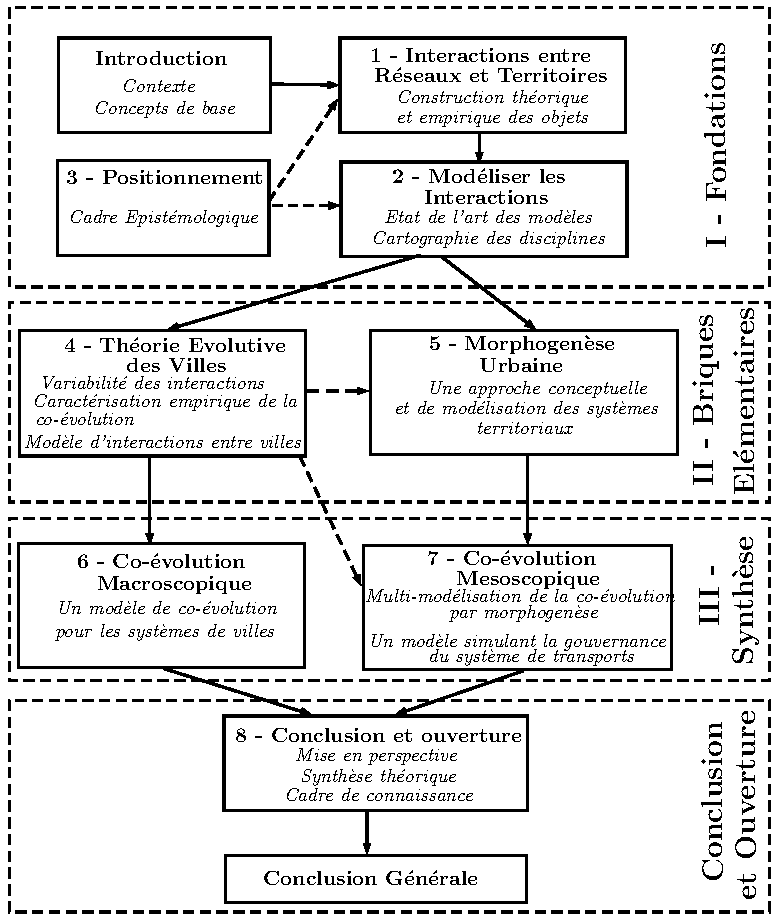
\includegraphics[width=\linewidth]{Figures/Theory/plan.pdf}
		
		\medskip
		
		\noun{Encadré : } \textit{Organisation générale du mémoire. Les flèches pleines donnent une dépendance directe (enchainement logique ou extensions), les flèches pointillées une dépendance indirecte (réutilisation de données ou de méthodes).}
		
	\end{mdframed}
\end{figure}
%%%%%%%%%%%


% \comment[AB]{intro = beau boulot !}

%\comment[FL]{Introduction \cn{关}
%\begin{itemize}
	%\item c'est seulement p11 que tu parles pour la premiere fois du sujet. Avant c'est de l'epistemo : pas une introduction a la these, mais une discussion - tres utile - sur les champs scientifiques. Garde cette discussion mais commence par une vraie introduction.[non, prefere garder cette strategie]
	%\item fin OK $\rightarrow$ et à positionner avant la partie epistemo.
%\end{itemize}
%}




%\paragraph{On linear reading}{Sur la lecture linéaire}

%%%%%%%
%% -- ON HOLD -- (depends on reflexive analysis - last appendix)


%\comment{expliquer notre position sur la difficulté d'une présentation linéaire, au delà de faire la synthèse. // bon bouquins y arrivent ? y réfléchir. la métaphore narrative intro/cl parties sera ce squelette linéaire. les deux approches sont compatibles.}


%\bpar{
%Research question and precise objects are deliberately fuzzy for now, as we postulate that the construction of a problematic can not be dissociated from the production of a corresponding theory. Reciprocally, it makes no sense to ask questions out of the blue, on objects that have been only partially or rapidly defined. Our preliminary question to enter the subject, that we can obtain from concrete cases such as our introducing anecdote or from preliminary literature review, is the following :
%}{
%Dans tous les cas, nous postulons que la construction d'une problématique ne peut être dissociée de la production d'une théorie correspondante. De manière réciproque, il n'y a aucun sens à poser des questions sorties de nulle part, sur des objets qui ont été seulement partiellement ou brièvement définis. Notre question préliminaire pour entrer dans le sujet, qu'on peut obtenir à partir de cas concrets comme l'anecdote introductive ou la revue de littérature préliminaire, est la suivante :
%}









\stars




%%%%%%%%%%%%%%%%%%%%%%%%%%%%%



%----------------------------------------------------------------------------------------


%%%%%%%%%%%%%%%%%%%%%%%%%%%%%
% Part I : Thematic subject construction and positioning
%
\ctparttext{This part set up foundations, constructing our research precise subject and questions from a thematic point of view, completed with a theoretical construction for framing at thematic and epistemological levels. We also provide methodological digressions, and a quantitative epistemological analysis completing the manual state of the art. \comment{(Arnaud) ça s'appelle lire}}
%
\part{Foundations}
%
% Introduction of part I


%\chapter*{Part I Introduction}{Introduction de la Partie I}
\chapter*{Introduction de la Partie I}


% to have header for non-numbered introduction
%\markboth{Introduction}{Introduction}


%\headercit{}{}{}


%---------------------------------------------------------------------------


















%---------------------------------------------------------------------------


\chapter*{Définitions prélimimaires}

Il est nécessaire de fixer pour commencer les définitions de notions qui joueront un rôle clé tout au long de notre raisonnement. Nous adoptons la stratégie suivante : les définitions données sont assez générales pour que les raffinements lorsqu'ils auront lieu précisent ces notions. Une fois qu'une notion aura été raffinée, son utilisation fera référence à l'ensemble de la profondeur (sauf utilisation particulière locale qui sera alors précisée explicitement). Cette stratégie permet d'une part d'alléger la lecture, et d'autre part favorise une lecture non-linéaire, vu que la profondeur complète ne sera pas nécessaire à toute étape pour une compréhension au premier ordre des connaissances construites. Lorsqu'une référence précise n'est pas donnée, les définitions sont inspirées de~\cite{hypergeo}. 


\subsection*{System}{Système}

Un \emph{Système} est composé ``\textit{d'un ensemble d'entités en interaction}''. Différentes formalisations équivalentes


\subsection*{Models}{Modèles et Ontologies}



\subsection*{Cities, System of Cities, Territories}{Villes, Systèmes de Villes, Territoires}




\subsection*{Causality}{Causalité}



\subsection*{Model Coupling}{Couplage de Modèles, Modèles Intégratifs}












%%%%%%%%%%%%%%%



%%%%%%%%%%%%%%%%%%%%%%%%%%%%%
% Chapter 1 : Thematic


% Chapter 




%\chapter{Interactions between Networks and Territories}{Interactions entre Réseaux et Territoires} % Chapter title
\chapter{Interactions entre Réseaux et Territoires}


\label{ch:thematic} % For referencing the chapter elsewhere, use \autoref{ch:name} 




%----------------------------------------------------------------------------------------

%\headercit{If you are embarrassed by the precedence of the chicken by the egg or of the egg by the chicken, it is because you are assuming that animals have always be the way they are}{Denis Diderot}{\cite{diderot1965entretien}}

%\headercit{Si la question de la priorit{\'e} de l'\oe{}uf sur la poule ou de la poule sur l'\oe{}uf vous embarrasse, c'est que vous supposez que les animaux ont {\'e}t{\'e} originairement ce qu'ils sont {\`a} pr{\'e}sent.
%}{Denis Diderot}{\cite{diderot1965entretien}}


\bigskip


\bpar{
This analogy is ideal to evoke the questions of causality and processes in territorial systems. When trying to tackle naively our preliminary question, some observers have qualified the identification of causalities in complex systems as ``chicken and egg'' problems : if one effect appears to cause another and reciprocally, how can one disentangle effective processes ? This vision is often present in reductionist approaches that do not postulate an intrinsic complexity in studied systems. The idea that Diderot suggests is the notion of \emph{co-evolution} that is a central phenomenon in evolutive dynamics of Complex Adaptive Systems as \noun{Holland} develops in~\cite{holland2012signals}. He links the notion of emergence (that is ignored in a reductionist vision), in particular the emergence of structures at an upper scales from the interactions between agents at a given scale, materialized generally by boundaries, that become crucial in the coevolution of agents at any scales : the emergence of one structure will be simultaneous with one other, each exploiting their interrelations and generated environments conditioned by their boundaries. We shall explore these ideas in the case of territorial systems in the following.
}{
Pour mieux visualiser les notions de causalités circulaires dans les systèmes complexes, et pourquoi celles-ci peuvent conduire à des paradoxes en apparence, l'image fournie par \noun{Diderot} dans~\cite{diderot1965entretien} est idéale : ``\textit{Si la question de la priorit{\'e} de l'\oe{}uf sur la poule ou de la poule sur l'\oe{}uf vous embarrasse, c'est que vous supposez que les animaux ont {\'e}t{\'e} originairement ce qu'ils sont {\`a} pr{\'e}sent}''. En voulant traiter naïvement des questions similaires induites par notre problématique introduite précédemment, certains ont qualifié les causalités au sein de systèmes complexes géographiques comme un problème ``de poule et {\oe}uf'' : si un effet semble causer l'autre et réciproquement, est-il possible et même pertinent de vouloir isoler les processus correspondants ? Cette question est bien connue des planificateurs des transports, comme le rappelle la notion des ``effets structurants'' qui fait débat depuis un certain temps au moins dans la communauté scientifique \comment[FL]{non cela va trop vite}. Une vision simplifiée, selon laquelle on peut attribuer des rôles systématiques à une composante particulière, est souvent présente dans les approches réductionnistes qui ne postulent pas une complexité intrinsèque au sein des systèmes étudiés.\comment[FL]{mots pas clairs ; a la place : amener co-evolution} L'idée suggérée par \noun{Diderot} est celle de \emph{co-evolution} qui est un phénomène central dans les dynamiques évolutionnaires des Systèmes Complexes Adaptatifs comme \noun{Holland} élabore dans~\cite{holland2012signals}. Il fait le lien entre l'émergence de structures à une échelle supérieure par les interactions entre agents à une échelle donnée, en général concrétisée par un systèmes de limites\comment[FL]{pas clair}, qui devient cruciale pour la co-évolution des agents à toutes les échelles : l'émergence d'une structure sera simultanée avec une autre, chacune exploitant leur interrelations et environnements générés conditionnés par le système de limites.\comment[FL]{rupture : le fil n'est pas clair} Nous explorerons ces idées pour le cas des systèmes territoriaux par la suite. Ceux-ci illustrent parfaitement ces problématiques, et sont typiques de systèmes dans lesquels cette complexité\comment[FL]{laquelle} est cruciale pour une appréhension raisonnable des mécanismes impliqués dans leurs dynamiques. Un certain nombre d'illustrations concrètes\comment[FL]{de quoi ?} seront d'abord données pour formuler nos questionnements dans des contextes géographiques donnés.\comment[FL]{phrase inutile}
}



\bpar{
This introductive chapter aims to set up the thematic scene, the geographical context in which further developments will root. It is not supposed to be understood as an exhaustive literature review nor the fundamental theoretical basement of our work (the first will be an object of chapter~\ref{ch:quantepistemo} whereas the second will be earlier tackled in chapter~\ref{ch:theory}), but more as narration aimed to introduce typical objects and views and construct naturally research questions.
}{
Ce chapitre introductif est destiné à poser le cadre thématique, les contextes géographiques sur lesquels les développements suivants se baseront.\comment[FL]{plus haut} Il n'est pas supposé être compris comme une revue de littérature exhaustive ni comme les fondations théoriques fondamentales de notre travail, le premier point étant l'objet du chapitre~\ref{ch:modelinginteractions} tandis que le second sera traité systématiquement dans le chapitre~\ref{ch:theory} lorsque le recul nécessaire aura été progressivement construit. Il doit plutôt être lu comme une construction narrative ayant pour but d'introduire nos objets et positions d'étude.\comment[FL]{cela sera dans l'intro generale} La notion de co-évolution est particulièrement pertinente\comment[FL]{oui : a remonter} pour comprendre les interactions entre territoires et réseaux. Dans une première section~\ref{sec:networkterritories}, nous préciserons l'approche prise de l'objet territoire, et dans quelle mesure celui-ci naturellement implique la considération des réseaux de transport pour la compréhension des dynamiques couplées. Ces considérations abstraites seront illustrées par des cas d'étude concrets dans la deuxième section~\ref{sec:casestudies}, choisis très différents pour comprendre les enjeux d'universalité sous-jacents. Enfin, dans la troisième section~\ref{sec:qualitative},des éléments d'observation de terrain effectués en Chine préciseront encore ces exemples aux échelles microscopique et mesoscopique. \comment[FL]{reprendre}
}



\stars


\textit{Ce chapitre est entièrement inédit.}\comment[FL]{ne pas dire cela}[(JR) permet d'avoir une unite avec les autres chapitres.]







%-------------------------------




























%
% 1.1 Network and Territories



\newpage


%-------------------------------


\section{Territories and Networks}{Territoires et Réseaux}

\label{sec:networkterritories}


%-------------------------------


Nous commençons par une construction plus précise des concepts mobilisés, qui permet de comprendre comment les concepts de territoire et de réseau sont rapidement en interdépendance forte, impliquant une importance ontologique des interactions entre les objets correspondants. Nous verrons que les territoires impliquent l'existence de réseaux, mais que réciproquement ceux-ci les influencent également. Un développement plus particulier sur les propriétés des réseaux de transport permet d'amener progressivement une vision précise de la \emph{co-évolution}, que nous prendrons jusque là dans son sens préliminaire donné précédemment, c'est à dire l'existence de relations causales circulaires entre réseaux de transports et territoires.


\subsection{Territories and Networks : There and Back Again}{Territoires et Réseaux : \emph{There and Back Again}}

Le voyage conceptuel que nous proposons d'entreprendre sera digne de celui de Bilbo en Terre du Milieu, partant du Territoire (dont la Conté est pour nous une allégorie) pour y revenir après une boucle naturelle par les Réseaux.

\subsubsection{Territories}{Territoires}


\bpar{
The notion of territory can be taken as a basis to explore the scope of geographical objects we will study. In Ecology, a territory corresponds to a spatial extent occupied by a group of agents or more generally an ecosystem. \emph{Human Territories} are far more complex in the sense of semiotic representations of these that are a central part in the emergence of societies. For \noun{Raffestin} in~\cite{raffestin1988reperes}, the so-called \emph{Human Territoriality} is the ``conjonction of a territorial process with an informational process'', what means that physical occupation and exploitation of space by human societies is not dissociable from the representations (cognitive and material) of these territorial processes, driving in return its further evolutions. In other words, as soon as social constructions are assumed in the constitution of human settlements, concrete and abstract social structures will play a role in the evolution of the territorial system, through e.g. propagation of information and representations, political processes, conjonction or disjonction between lived and perceived territory.
}{
Le concept\footnote{Nous utiliserons le terme \emph{concept} pour des connaissances construites, plutôt que celui de \emph{notion}, qui suivant~\cite{raffestin1978construits} est plus proche d'une information empirique. Cette distinction peut être mise en perspective avec les domaines de connaissance théorique et empirique de~\cite{livet2010}, que nous approfondissons en~\ref{sec:knowledgeframework}.} de \emph{Territoire}, que nous avons introduit précédemment par ceux de Ville et de Système de Ville, sera central à nos raisonnements et nécessite d'être approfondi et enrichi. En Ecologie Spatiale, un groupe d'agents ou plus généralement un écosystème occupe une certaine étendue spatiale~\cite{tilman1997spatial}, qu'on peut identifier comme notion de territoire. Les territoires des sociétés humaines impliquent des dimensions supplémentaires, par exemple par l'importance de leur représentations sémiotiques\footnote{c'est à dire des signes marquants les territoires et leur sens, mais aussi leur représentations, cartographiques par exemple}. Celles-ci jouent un rôle significatif dans l'émergence des constructions sociétales, dont la genèse est profondément liée à celle des systèmes urbains. Selon~\cite{raffestin1988reperes}, la \emph{Territorialité Humaine} est ``la conjonction d'un processus territorial avec un processus informationnel'', ce qui implique que l'occupation physique et l'exploitation de l'espace par les sociétés humaines sont complémentaires des représentations (cognitives et matérielles) de ces processus territoriaux, qui influent en retour sur leur évolution.
}

\bpar{}{
En d'autres termes, à partir de l'instant où les constructions sociales déterminent la constitution des établissements humains, les structures sociales abstraites et concrètes joueront un rôle dans l'évolution des territoires, et ces deux objets seront intimement liés. Des exemples de tels liens se retrouvent à travers la propagation d'informations et de représentations, par des processus politiques, ou encore par la correspondance plus ou moins effective entre territoire vécu et territoire perçu. Une illustration concrète est donnée par une vision simplifiée de la construction de la Métropole du Grand Paris, qui témoigne des ajustements successifs des territoires administratifs (émergence d'un nouveau niveau de gouvernance), des territoires fonctionnels (partiellement par l'évolution des possibilités d'accessibilité), des territoires perçus (dépassement de l'opposition Paris-banlieue), des territoires vécus (nouvelles pratiques de mobilité ou de mobilité résidentielle pouvant être induites en partie par les dynamiques territoriales et du nouveau réseau de transport), l'ensemble de ces processus étant liés de manière complexe et ceux-ci étant loin d'être systématiques. Un territoire est ainsi compris comme une structure sociale organisée dans l'espace, qui comprend ses artefacts concrets et abstraits.
}


% \comment[FL]{je ne suis pas sur que tu doives garder cette digression}[removed]
% Une étendue spatiale imaginaire avec des ressources potentielles qui n'aurait jamais connu de contact avec l'humain ne pourra pas être un territoire si elle n'est pas habitée, imaginée, vécue, exploitée, même si ces ressources pourraient être potentiellement exploitée le cas échéant. En effet, ce qui est considéré comme une ressource (naturelle ou artificielle) dépendra de la société (par exemple de ses pratiques et de ses capacités technologiques).



% complementarité du point de vue de la theorie evolutive : boucler la boucle ?

\bpar{
Although this approach does not explicitly give the condition for the emergence of a seminal system of aggregated settlements (i.e. the emergence of cities), it insists on the role of these that become places of power and of creation of wealth through exchange. But the city has no existence without its hinterland and the territorial system can not be summarized by its cities as a system of cities. There is however compatibility on this subsystem between \noun{Raffestin} approach to territories and \noun{Pumain}'s evolutive theory of urban systems~\cite{pumain2010theorie}, in which cities are viewed as an auto-organized complex dynamical systems, and act as mediators of social changes : for example, cycles of innovation occur within cities and propagate between them. Cities are thus competitive agents that co-evolve (in the sense given before). The territorial system can be understood as a spatially organized social structure, including its concrete and abstract artifacts. A imaginary free-of-man spatial extent with potential ressources will not be a territory if not inhabited, imagined, lived, and exploited, even if the same ressources would be part of the corresponding habited territorial system. Indeed, what is considered as a ressource (natural or artificial) will depend on the corresponding society (e.g. of its practices and technological potentialities).
}{
Cette approche du territoire est compatible avec la définition préliminaire que nous en avions prise, qui vient alors la renforcer. L'approche de \noun{Raffestin} insiste sur le rôle des villes comme lieu de pouvoir (au sens d'un lieu rassemblant des processus décisionnel et de contrôle socio-économique) et de création de richesse au travers des échanges et interactions\footnote{Une interaction sera comprise dans son sens le plus général, comme une action réciproque de plusieurs entités l'une sur l'autre. Celle-ci peut être physique, informationnelle, transformer les entités, etc. Voir~\cite{morin1976methode} pour une construction complète et complexe du concept, en lien intime avec celui d'organisation.} (sociaux, économiques). La ville n'a cependant pas d'existence sans son hinterland, ce qu'on interpréter comme le \emph{territoire d'une ville}\footnote{Même si une correspondance exacte entre territoires et villes n'est probablement qu'une simplification de la réalité, puisque les territoires peuvent s'entremêler à différentes échelles, selon différentes dimensions. Une lecture par lieux centraux de type \noun{Christaller}~\cite{banos2011christaller} permet de se faire une image conceptuelle de cette correspondance. Des définitions fonctionnelles comme celles des aires urbaines de l'Insee, qui définit l'aire autour d'un pôle dépassant une taille critique (10000 emplois) par les communes dont un seuil minimal d'actifs travaillent dans le pôle (40\%) - voir \url{https://www.insee.fr/fr/metadonnees/definition/c2070}, est une approche possible. La sensibilité des propriétés du système urbain à ces paramètres est testée par~\cite{2015arXiv150707878C}. La définition de la ville est alors intimement liée à celle de ses territoires, et celle du système urbain à l'ensemble des territoires.}. Cette correspondance permet de lire l'ensemble des territoires au prisme du système de villes, comme développé par la Théorie Evolutive des Villes~\cite{pumain2010theorie}. Celle-ci interprète les villes comme des systèmes complexes auto-organisés, qui agissent comme des médiateurs du changement social : par exemple, les cycles d'innovation s'initialisent au sein des villes et se propagent entre elles (voir~\ref{app:sec:patentsmining} pour une entrée empirique sur la notion d'innovation) : cela permet de comprendre le territoire comme un espace des flux, ce qui permettra d'introduire la notion de réseau comme nous le verrons plus loin. Les villes sont par ailleurs vues comme des agents compétitifs qui co-évoluent~\cite{paulus2004coevolution}, ce qui permet de préfigurer également l'importance de la co-évolution pour les dynamiques territoriales.
}



% approche historique et point de vue complementaires

\bpar{

}{
On a ainsi deux approches complémentaires du territoire qui nous permettent de considérer des territoires humains structurés par les systèmes de villes\footnote{Ces visions complémentaires du territoire peuvent également être enrichies par une perspective historique. \cite{di1998espace} procède à une analyse historique des différentes conceptions de l'espace (qui aboutissent entre autres à l'espace vécu, l'espace social et l'espace classique de la géographie) et montre comment leur combinaison forme ce que \noun{Raffestin} décrit comme territoires. \cite{giraut2008conceptualiser} rappelle les différents usages récents qui ont été faits de la notion de territoire, de la géographie culturelle où il a plus été utilisé par effet de mode, à la géopolitique où c'est un terme bien spécifique lié aux structures de gouvernance, en passant par des utilisations où il sert plus de concept, et dégage l'aspect interdisciplinaire d'un objet capturant une certaine complexité des systèmes étudiés.}.
}



% transition

\bpar{
A crucial aspect of human settlements that were studied in geography for a long time, and that relate with the previous notion of territory, are \emph{networks}. Let see how we can switch from one to the other and how their definition may be indissociable.
}{
Par ailleurs, un aspect central des établissements humains qui a une longue tradition d'étude en géographie, et qui est directement relié au concept de territoire, est celui des \emph{réseaux}. Nous allons préciser leur définition et voir comment le passage de l'un à l'autre est intrinsèque aux approches que nous en prenons.
}



\subsubsection{Networks}{Réseaux}


% definition des réseaux de manière generale


Un \emph{réseau} doit être compris au sens large d'une mise en relation entre entités d'un système, qui peuvent être vus comment relations abstraites, liens, interactions. \cite{haggett1970network} postule que l'existence d'un réseau est nécessairement liée à celle de flux\footnote{On définit le flux comme un échange matériel (personnes, marchandises, matières premières) ou immatériel (information) entre deux entités.}, et rappelle la représentation topologique sous forme de graphe de tout système géographique dans lequel circulent des flux entre des entités ou des lieux qui sont abstraits sous la forme de noeuds, reliés par des liens. Les liens du réseau disposent alors d'une \emph{capacité}, qui traduit leur capacité à transporter les flux (qui peut également être définie de manière équivalence comme \emph{impédance}). L'analyse topologique révèle déjà un certain nombre de propriétés du système, mais \cite{haggett1970network} précise l'importance de la spatialisation du réseau, incluse dans les propriétés de ses noeuds (localisation) et de ses liens (localisation, impédance), pour la compréhension des dynamiques dans le réseau (flux) ou du réseau lui-même (croissance du réseau). Cette spécificité a été rappelée par~\cite{barthelemy2011spatial} qui met en perspective les domaines empiriques concernés par les réseaux spatiaux, certains modèles de croissance de réseau, et certains modèles de processus dans les réseaux : par exemple, les structures topologiques, ou les processus de diffusion seront très contraints par le caractère spatial.

%\comment[AB]{Bien :)}

% Les territoires impliquent des réseaux potentiels, selon Dupuy


\bpar{
We paraphrase \noun{Dupuy} in~\cite{dupuy1987vers} when he proposes elements for ``a territorial theory of networks'' based on the concrete case of Urban Transportation Networks. This theory sees \emph{real networks} (i.e. concrete networks, including transportation networks) as the materialization of \emph{virtual networks}. More precisely, a territory is characterized by strong spatio-temporal discontinuities induced by the non-uniform distribution of agents and ressources. These discontinuities naturally induce a network of ``transactional projects'' that can be understood as potential interactions between elements of the territorial system (agents and/or ressources). For example today, people need to access the ressource of employments, economic exchanges operate between specialized production territories.
}{
Pour approfondir le concept de réseau en appuyant sur sa forte interdépendance avec celui de Territoire, nous reprenons~\cite{dupuy1987vers} qui propose des éléments pour une ``théorie territoriale des réseaux'' s'inspirant du cas concret d'un réseau de transport urbain. Cette théorie distingue les \emph{réseaux réels}\footnote{Les réseaux réels contiennent une catégorie qu'on peut désigner comme réseaux concrets, matériels ou physiques - nous utiliserons ces termes de manière interchangeable par la suite, à laquelle les réseaux de transport appartiennent; d'autres catégories comme les réseaux sociaux sont également des réseaux réels sur lesquels nous ne nous attarderons pas.} et les \emph{réseaux virtuels}, eux-mêmes induits entre autre par la configuration territoriale. Les réseaux réels sont la matérialisation de réseaux virtuels. Plus précisément, un territoire est caractérisé par de fortes discontinuités spatio-temporelles induites par la distribution non-uniforme des agents et des ressources. Ces discontinuités induisent naturellement un réseau d'interactions potentielles entre les éléments du système territorial, notamment des agents et des ressources. \cite{dupuy1987vers} désigne ces interactions potentielles comme \emph{projets transactionnels}. Celles-ci induisent la notion de \emph{potentiel d'interaction}, c'est à dire une propriété de l'espace dont les interactions dérivent\footnote{Etant donné tout champ vectoriel de classe $\mathcal{C}^1$ sur $\mathbb{R}^3$, le théorème d'\noun{Helmoltz} fournit un potentiel vecteur et un potentiel scalaire dont ce champ dérive par rotationnel et gradient. Cela justifie dans le cas particulier d'un tel point de vue formel le passage d'un champ d'interaction entre agents à un champ de potentiel.}. Par exemple, de nos jours les actifs ont besoin d'accéder à la ressource qu'est l'emploi, et des échanges économiques s'effectuent entre les différents territoires qui peuvent être plus ou moins spécialisés dans les productions de différents types.
}

%\comment[FL]{la encore au bout de plusieurs lignes dont on ne comprend plus l'objet, il est difficile de suivre}[(sur reseau reels) -> reel/concret en footnote, plus court et comprehensible]

% \comment[AB]{rotation ?}[non, bien $\vec{rot}\vec{A}$ - yes preciser que bien un cas bien particulier]



\subsubsection{Real networks}{Réseaux réels}

% Les réseaux potentiels se transforment en réseaux réels sous certaines conditions.
%. -> effet des territoires sur les réseaux

\bpar{
The potential interaction network is concretized as offer adapts to demand, and results of the combination of economic and geographical constraints with demand patterns, in a non-linear way through agents designed as \emph{operators}. This process is not immediate, leading to strong non-stationarity and path-dependance effects : the extension of an existing network will depend on previous configuration, and depending on involved time scales, the logic and even the nature of operators may have evolved.
}{
Dans certains cas, un réseau potentiel peut se matérialiser en réseau réel. La question sous-jacente est alors de savoir si le champ de potentiel des territoires est en partie à l'origine de cette matérialisation, si celle-ci est totalement indépendante, ou si la dynamique des deux est fortement couplée, en d'autres termes en co-évolution. La matérialisation résultera généralement de la combinaison de contraintes économiques et géographiques avec des motifs de demande, de manière non-linéaire. Un tel processus est loin d'être immédiat, et conduit à de forts effets de non-stationnarité et de dépendance au chemin\footnote{La non-stationnarité spatiale consiste en la dépendance de la structure de covariance des processus à l'espace, tandis que la dépendance au chemin traduit le fait que les trajectoires prises par le passé influencent fortement les trajectoires actuelles du système.} : l'extension d'un réseau existant dépendra de la configuration précédente, et selon les échelles de temps impliquées, la logique et même la nature des opérateurs, c'est à dire des agents participant à sa production, peut avoir évolué.
}


% Les exemples de trajectoires concrètes peuvent être très variées : \comment[FL]{TB}


\bpar{
}{
Les exemples de trajectoires concrètes peuvent être très variées : \cite{kasraian2015development} montre par exemple dans le cas de la Randstad sur le temps long, une première période pendant laquelle le réseau ferré s'est développé pour suivre le développement urbain, tandis que des effets inverses ont été constaté plus récemment. A une échelle urbaine sur le temps long, la dépendance au chemin est montrée pour Boston par~\cite{block2012hysteresis} puisque l'environnement bâti et la distribution de la population apparaissent comme fortement dépendants des lignes de tramway antérieures même lorsqu'elles n'existent plus : la façon dont la ligne de transport change l'espace urbain s'opère dans les dynamiques immédiates mais aussi sur le temps long par des effets de renforcement ou à cause de l'inertie du bâti par exemple.
}

\bpar{
The presence of a human territory necessarily imply the presence of abstract interaction networks and concrete networks used for transportation of people and ressources (including communication networks as information is a crucial ressource). Depending on regime in which the considered system is, the respective role of different networks may be radically different. Following \noun{Duranton} in \cite{duranton1999distance}, pre-industrial cities were limited in growth because of limitations of transportation networks. Technological progresses have lead to the end of these limitations and the preponderance of land markets in shaping cities (and thus a role of transportation network as shaping prices through accessibility), and recently to the rising importance of telecommunication networks that induce a ``tyranny of proximity'' as physical presence is not replaceable by virtual communication.
}{
Ainsi, l'existence d'un territoire humain implique nécessairement la présence de réseaux d'interactions abstraites, et les réseaux concrets sont cruciaux pour transporter les individus et les ressources (incluant les réseaux de communication puisque l'information est une ressource essentielle~\cite{morin1976methode}), mais les processus d'établissement de ceux-ci sont difficiles à identifier de manière générale. Notre choix ontologique de positionnement dans la théorie de \noun{Dupuy}, donne une place privilégiée aux relations entre réseaux et territoires, puisqu'il induit dans la construction des objets même une imbrication complexe entre ceux-ci.
}

% \comment[FL]{tres flou. pas du niveau chap 1 a mon avis}[reformulé, et si chap. 1 - c'est bien l'approche prise qui permet interdep dès l'ontologie]

% le contexte socio-eco/techno conditionne fortement la facon dont les réseaux agissent sur les territoires.

\bpar{
}{
Le statut du réseau par rapport au territoire est d'autre part fortement conditionné par le contexte socio-économique et technologique. Selon \noun{Duranton}~\cite{duranton1999distance}, un facteur influençant la forme des villes pré-industrielles était la performance des réseaux de transport. Les progrès technologiques, conduisant à une baisse des coûts de transport, ont induit un changement de régime, ce qui a mené à une prépondérance du marché foncier dans la formation des villes (et par conséquent un rôle des réseaux de transport qui déterminent les prix par l'accessibilité), et plus récemment à une importance croissante des réseaux de télécommunication ce qui a induit une ``tyrannie de la proximité'' puisque la présence physique n'est pas remplaçable par une communication virtuelle~\cite{duranton1999distance}.
}

% On s'attendra ainsi à l'existence de multiples processus d'interaction, potentiellement superposables de manière complexe.\comment[FL]{creux pour l'instant}[suppr]




% Transition

\bpar{
This territorial approach to networks seems natural in geography, since networks are studied conjointly with geographical objects with an underlying theory, in opposition to network science that studies brutally spatial networks with few thematic background~\cite{ducruet2014spatial}.
}{
Cette approche territoriale des réseaux semble naturelle en géographie, puisque les réseaux sont étudiés conjointement avec des objets géographiques qu'ils connectent, en opposition aux travaux théoriques sur les réseaux complexes qui les étudient de manière relativement déconnectée de leur fond thématique~\cite{ducruet2014spatial}.
}





\subsubsection{Networks shaping territories ?}{Des réseaux qui façonnent les territoires ?}

% Effets des réseaux sur les territoires ? -> approfondir le debat des effets structurants

\bpar{
However networks are not only a material manifestation of territorial processes, but play their part in these processes as they evolution may shape territories in return. In the case of \emph{technical networks}, an other designation of real networks given in~\cite{offner1996reseaux}, many examples of such feedbacks can be found : the interconnectivity of transportation networks allows multi-scalar mobility patterns, thus shaping the lived territory. At a smaller scale, changes in accessibility may result in an adaptation of a functional urban space. Here emerges again an intrinsic difficulty : it is far from evident to attribute territorial mutations to some network evolutions and reciprocally materialization of a network to precise territorial dynamics. Coming back to Diderot should help, in the sense that one must not consider network nor territories as independent systems that would have causal relationships but as strongly coupled components of a larger system. These potential retroactions of networks on territories does not necessarily act on concrete components : \noun{Claval} shows in~\cite{claval1987reseaux} that transportation and communication networks contribute to the collective representation of territories by acting on territorial belonging feeling.
}{
Cependant les réseaux ne sont pas seulement une manifestation matérielle de processus territoriaux, mais jouent également leur rôle dans ces processus comme leur évolution peut influencer l'évolution des territoires en retour. Il emerge alors une difficulté intrinsèque : il n'est pas évident d'attribuer des mutations territoriales à une évolution du réseau et réciproquement la matérialisation d'un réseau à des dynamiques territoriales précises, et différents facteurs exogènes rentrent par ailleurs en compte, comme le prix de l'énergie ou les technologies existantes dans le cas de l'effet du réseau sur les territoires par exemple. Dans le cas des \emph{réseaux techniques}, une autre désignation des réseaux concrets donnée dans~\cite{offner1996reseaux}, de nombreux exemples de tels retroactions peuvent être mis en évidence : une accessibilité accrue peut être un facteur favorisant la croissance urbaine, ou bien l'interconnexion de différents réseaux de transport permet une extension significative de la portée des déplacements. A une plus petite échelle, des changements de l'accessibilité peuvent induire des relocalisations de différentes composantes urbaines. Ces retroactions des réseaux sur les territoires n'agissent pas nécessairement sur des composantes concretes : \noun{Claval} montre dans~\cite{claval1987reseaux} que les réseaux de transport et de communication contribuent à la représentation collective d'un territoire en agissant sur un sentiment d'appartenance, qui peut alors jouer un rôle crucial dans l'émergence d'une dynamique régionale fortement cohérente. Développons d'abord plus en détail les possibles influences des réseaux sur les territoires.
}


\bpar{
The confusion on possible simple causal relationships has fed a scientific debate that is still active. Methodologies to identify so-called \emph{structural effects} of transportation networks were proposed by planners in the seventies~\cite{bonnafous1974detection,bonnafous1974methodologies}.
}{
La confusion autour de possibles relations causales simples a nourri un débat scientifique encore actif aujourd'hui. La question sous-jacente repose sur des attributions plus ou moins déterministes d'impact d'infrastructures ou d'un nouveau mode de transport sur des transformations territoriales. On peut trouver des précurseurs de ce raisonnement dès les années 1920 : \noun{McKenzie}, de l'école de Chicago, parle dans~\cite{burgess1925city} des `` modifications des formes du transport et de la communication comme facteurs déterminants des cycles de croissance et de déclin [des territoires]'' (p. 69). Des méthodologies pour identifier ce qui est alors nommé \emph{effets structurants} des réseaux de transport ont été développées pour la planification dans les années 1970 : \cite{bonnafous1974methodologies} situe le concept d'effet structurant dans le cadre d'une logique d'utilisation de l'offre de transport comme outil d'aménagement (les alternatives étant le développement d'une offre pour répondre à une congestion du réseau, et le développement simultané d'une offre et d'un aménagement associé). Ces auteurs identifient du point de vue empirique des effets directs d'une nouvelle offre sur le comportement des agents, sur les flux de transport et des possibles inflexions sur les trajectoires socio-économiques des territoires concernés. \cite{bonnafous1974detection} développe une méthode pour identifier de tels effets par modifications de la classe des communes dans une typologie établie a posteriori. Plus récemment, \cite{bonnafous2014observatoires} a proposé la mise en place \emph{d'observatoires permanents} des territoires pour rendre plus robustes ce type d'analyse, en permettant un suivi continu de l'évolution des territoires les plus concernés par l'emprise d'une nouvelle infrastructure.
}


\bpar{
It took some time for a critical positioning on unreasoned and decontextualized use of these methods by planners and politics generally to technocratically justify transportation projects, that was first done by \noun{Offner} in~\cite{offner1993effets}. Recently the special issue~\cite{espacegeo2014effets} on that debate recalled that on the one hand misconceptions and misuses were still greatly present in operational and planning milieus as~\cite{crozet:halshs-01094554} confirmed, and on the other hand that a lot of scientific progresses still need to be made to understand relations between networks and territories as \noun{Pumain} highlights that recent works gave evidence of systematic effects on very long time scales (as e.g. the work of \noun{Bretagnolle} on railway evolution, that shows a kind of structural effect in the necessity of connectivity to the network for cities to ``stay in the game'', but that is not fully causal as not sufficient).
}{
Selon \cite{offner1993effets} qui reprend des idées déjà évoquées par~\cite{franccois1977autoroutes} par exemple, il s'est par la suite développé un usage non raisonné et hors contexte de ces méthodes par les planificateurs et les politiques qui les mobilisaient généralement pour justifier des projets de transports de manière technocratique : justifiant d'un effet direct d'une nouvelle infrastructure sur le développement local (par exemple économique), les élus sont en mesure de demander des financements et de légitimer leur action auprès des contribuables. \cite{offner1993effets} insiste sur la nécessité d'un positionnement critique sur ces enjeux, rappelant qu'il n'existe pas de démonstration scientifique d'un effet qui serait systématique. Une édition spéciale de l'Espace Géographique sur ce débat~\cite{espacegeo2014effets} a rappelé d'une part que de telles croyances était encore largement présentes aujourd'hui dans les milieux opérationnels de la planification, ce qui peut s'expliquer par exemple par le besoin de justifier l'action publique, et d'autre part qu'une compréhension scientifique des relations entre réseaux et territoires est encore en pleine construction.
}


\bpar{}{
Une illustration concrète d'actualité permet de se faire une image de cette instrumentalisation : les débats en juillet 2017 relatifs à l'ouverture des LGV Bretagne et Sud-Ouest ont montré toute l'ambiguïté des positions, des conceptions, des imaginaires à la fois des politiques mais aussi du public : inquiétude quant à la spéculation sur l'immobilier dans les quartiers de gare, questionnements des pratiques de mobilité quotidienne mais aussi sociale\footnote{Voir par exemple \url{http://www.liberation.fr/futurs/2017/07/02/immobilier-plus-de-parisiens-comment-les-bordelais-voient-l-arrivee-de-la-lgv_1580776}, ou \url{http://www.lemonde.fr/big-browser/article/2017/10/24/a-bordeaux-une-fronde-anti-parisiens-depuis-l-ouverture-de-la-ligne-a-grande-vitesse_5205282_4832693.html} pour une réaction ``à chaud'' de divers acteurs locaux, témoignant d'un impact au minimum sur les représentations. Par exemple, les Bordelais semblent craindre l'arrivée de Parisiens en recherche d'un logement moins cher et de meilleurs conditions de vie, ce qui pourrait augmenter les prix au moins aux environs de la gare.}. La complexité et la portée des sujets montrent bien la difficulté d'une compréhension systématique d'effets du transport sur les territoires.
}

% \comment[FL]{tu ne dis rien ! alors autant ne pas en parler}[si, en footnote]



\subsubsection{Territorial Systems}{Systèmes Territoriaux}


\bpar{
This detour from territories, to networks and back again, allows us to give a preliminary definition of a territorial system that will be the basis of our following theoretical considerations. As we emphasized the role of networks, the definition takes it into account.
\textbf{Preliminary Definition.} \textit{A territorial system is a human territory to which both interaction and real networks can be associated. Real 
 networks are a component of the system, involved in evolution processes, through multiples feedbacks with other components at various spatial and temporal scales.}
 This reading of territorial systems is conditional to the existence of networks and may discard some human territories, but it is a deliberate choice that we justify by previous considerations, and that drives our subject towards the study of interactions between networks and territories.
}{
Cet aperçu introductif, des territoires aux réseaux, nous permet ainsi de clarifier notre approche des systèmes territoriaux qui sera sous-jacente dans l'ensemble de la suite. Une prise en compte des diverses rétroactions potentielles des réseaux pour la compréhension des territoires est suggérée par un retour à la citation de Diderot ayant introduit le sujet devrait aider à ce point, au sens où il ne faut pas considérer le réseau ni les territoires comme des systèmes indépendants qui s'influenceraient soit l'une soit l'autre par des relations causales en sens unique, mais comme des composantes fortement couplées d'un système plus large, et donc étant en relations causales circulaires. Selon les composantes ainsi que l'échelle considérées, différentes manifestations de celles-ci pourront être observables, et il existera des cas où il y apparemment influence de l'une sur l'autre, d'autres où les influences sont simultanées, ou encore d'autres ou aucune relation n'est observable de manière significative.
}

% \comment[FL]{c'est au coeur de ta demarche. mieux expliquer (et nuancer)}

\bpar{}{
Comme nous avons mis en exergue le rôle des réseaux dans de nombreux aspects des dynamiques territoriales, nous proposons une définition des systèmes territoriaux les incluant explicitement. Nous considérons un \emph{Système Territorial} comme un \emph{territoire humain qui contient à la fois des réseaux d'interactions et des réseaux réels}. Les réseaux réels, et plus particulièrement les réseaux concrets\footnote{Qui comme nous l'avons vu précédemment sont des réseaux réels matérialisés.}, sont une composante à part entière du système, jouant dans les processus d'évolution, au travers de multiples retroactions avec les autres composantes à plusieurs échelles spatiales et temporelles.
}

% Cette lecture des systèmes territoriaux est conditionnée à l'existence des réseaux\comment[FL]{je penche pour supprimer ce genre de phrase} et pourrait écarter certains territoires humains%\footnote{Quoique nous doutions de cette affirmation et soyons convaincus \emph{qu'il n'existe de territoire humain sans réseau d'interaction}, il est évidemment impossible de prouver cette assertion.\comment[FL]{digression inutile, de plus il existe beaucoup de territoires humains sans reseaux : une chambre, un terrain de foot, un desert, etc.}}, mais il s'agit d'un choix délibéré justifié par les considérations précédentes, et qui confirme le positionnement de notre sujet vers l'étude des interactions entre réseaux et territoires.


\bpar{}{
Le réseau n'est pas nécessairement une composante en tant que telle du territoire, mais bien du \emph{Système Territorial} en notre sens\footnote{Ce choix ontologique n'est pas anodin et appuie la dialectique entre réseaux et territoires. Partant de l'époque lointaine où les réseaux physiques n'existaient pas, l'émergence d'un territoire humain, que nous supposons équivalent à un réseau d'interactions, induit la mise en place de la dialectique diachronique complexe entre réseaux physiques et territoires humains. On peut ainsi lire la genèse du système territorial comme une boucle morinienne~\cite{morin1976methode}, dans laquelle on entre par le territoire initial puis qui se boucle du réseau physique aux composantes territoriales pour former le système territorial (donc le territoire dans la majorité des cas) de la manière récursive suivante :\\Territoire initial $\rightarrow$ Territoire $=$ \tikzmark{Configuration} territoriale$\rightarrow$ Réseau \tikzmark{physique}\arrow{physique}{Configuration}\\}. Cette vision rejoint le positionnement de \cite{dupuy1985systemes} qui introduit le territoire comme ``produit d'une dialectique'' entre composantes territoriales et réseaux. Notons le raccourci sémantique pour désigner les composantes du système territorial qui ne sont pas les réseaux et qui interagissent avec celui-ci, par le terme de territoire. Celles-ci dépendent des ontologies et des échelles considérées, comme nous le verrons par la suite, et peuvent aller des agents microscopiques aux villes elle-mêmes. Comme nous le verrons aussi par la suite (voir~\ref{sec:modelingsa}), il existe des paradigmes où ce raccourci n'est pas fait, comme dans le cas particulier des interactions entre transport et usage du sol ou les entités sont spécifiques. Mais il est fait si on reste à un cadre plus général, comme en témoigne l'un des ouvrages de référence sur le sujet~\cite{offner1996reseaux}\footnote{Lorsque \cite{amar1985essai} propose un modèle conceptuel de morphogenèse des réseaux, il désigne les composantes territoriales par ``Le Monde'', ce qui n'apporte pas de solution au problème sémantique. Le parti pris de garder le territoire, au sein du territoire, suggère une récursivité, et donc une complexité dans la générativité du système~\cite{morin1976methode}. La mobilisation du concept de morphogenèse à partir du Chapitre~\ref{ch:morphogenesis} suggère que cette récursivité serait plus que fortuite, mais bien intrinsèque au problème.}. Nous assumerons également ce raccourci de langage, en désignant par \emph{interactions entre réseaux et territoires} ou \emph{co-évolution entre réseaux et territoires}, les interactions ou la co-évolution entre les réseaux physiques et les composantes qu'ils relient, au sein d'un système territorial et donc d'un territoire.
}




\subsection{Transportation Networks}{Réseaux de Transport}


Nous précisons à présent le cas particulier des réseaux de transport et développons des concepts spécifiques associés qui joueront un rôle prépondérant dans la précision de notre problématique.


\subsubsection{Specificity of transportation networks}{Spécificités des réseaux de transport}


\bpar{
}{
Centraux aux discussions déjà évoquées sur les effets structurants des réseaux, les réseaux de transports jouent un rôle significatif dans l'évolution des territoires, mais il n'est évidemment pas question de leur attribuer des effets causaux déterministes. On parlera de manière générale de réseau de transport pour désigner l'entité fonctionnelle permettant un déplacement des agents et des ressources au sein et entre les territoires\footnote{On désigne ainsi à la fois l'infrastructure, mais aussi ses conditions d'exploitation, le matériel roulant, les agents exploitants.}. Même si d'autres types de réseaux sont également fortement impliqués dans l'évolution des systèmes territoriaux (voir par exemple les débats sur l'impact des réseaux de communication sur la localisation des activités économiques), les réseaux de transport conditionnent d'autres types de réseaux (logistique, échanges commerciaux, interactions sociales concrètes pour donner quelques exemples) et sont une entrée privilégiée en rapport aux motifs d'évolution territoriale, en particulier dans nos sociétés contemporaines pour lesquelles les réseaux de transport jouent un rôle privilégié~\cite{bavoux2005geographie}. Nous nous concentrerons ainsi par la suite uniquement sur les réseaux de transport.
}


\bpar{
Already evoked in relation to the question of structural effects of networks, transportation networks play a determining role in the evolution of territories. Although other types of networks are also strongly involved in the evolution of territorial systems (see e.g. the discussions of impacts of communication networks on economic activities), transportation networks shape many other networks (logistics, commercial exchanges, social concrete interactions to give a few) and are prominent in territorial evolution patterns, especially in our recent societies that has become dependent of transportation networks~\cite{bavoux2005geographie}. The development of French High Speed Rail network is a good illustration of the impact of transportation networks on territorial development policies. Presented as a new era of railway transportation, a top-down planning of totally novel lines was introduced as central for developments~\cite{zembri1997fondements}. The lack of integration of these new networks with existing ones and with local territories is now observed as a structural weakness and negative impacts on some territories have been shown~\cite{zembri2008contribution}. A review done in~\cite{bazin2011grande} confirms that no general conclusions on local effects of High Speed lines connection can be drawn although it keeps a strong place in imaginaries. These are examples of how transportation networks have both direct and indirect impacts on territorial dynamics.
}{
Le développement du réseau français à grande vitesse est une illustration du rôle des réseaux de transport sur les politiques de développement territorial. Présenté comme une nouvelle ère de transport sur rail, il s'agit d'une planification au niveau de l'Etat de lignes totalement nouvelles et relativement indépendantes de par leur vitesse deux fois plus élevée, selon la lecture de~\cite{zembri1997fondements}. La grande vitesse a été défendue par les acteurs politiques entre autres comme central pour le développement. L'articulation faible de ces nouveaux réseaux avec le réseau classique et avec les territoires locaux est à présent observé comme une faiblesse structurelle~\cite{zembri1997fondements} (c'est à dire conséquence de la structure du réseau tel qu'il a été planifié dans le Schéma Directeur de 1990), et des impacts négatifs sur certains territoires, comme par la suppression de dessertes intermédiaires sur les lignes classiques empruntées par le TGV, qui contribue à un accroissement de l'effet tunnel\footnote{L'effet tunnel désigne le processus de télescopage du territoire traversé par une infrastructure, celle-ci n'étant utilisable à partir de celui-ci.} ont été montrés~\cite{zembri2008contribution}. Une revue faite dans~\cite{bazin2011grande} confirme qu'aucune conclusion générale sur des effets locaux d'une connection à une ligne à grande vitesse ne peut être tirée, bien que ce sésame garde une place conséquente dans les imaginaires des élus\footnote{Mais des conclusions particulières existent dans certains cas : par exemple un effet positif de la LGV Sud-Est sur la fréquentation touristique de villes moyennes intermédiaires comme Montbard ou Beaune~\cite{bonnafous1987regional} ; ou le positionnement de Lille comme métropole européenne dans lequel les connexions LGV ont joué~\cite{giblin2004lille}.}. Le développement des différentes Lignes à Grande Vitesse s'inscrit dans des contextes territoriaux très différents, et il est dans tous les cas délicat d'interpréter des processus en les sortant de leur contexte : par exemple, les lignes LGV Nord et LGV Est s'inscrivent dans des échelles européennes plus vastes que la LGV Bretagne ouverte en juillet 2017\footnote{La ligne LGV Nord relie Paris à Lille puis Calais (ouverte entièrement en 1997), et s'inscrit dans la liaison avec Londres, Bruxelles et Amsterdam. La LGV Est relie Paris à Strasbourg (ouverte partiellement en 2007, puis entièrement en 2016) et permet de desservir le Luxembourg et l'Allemagne. La LGV Bretagne, ouverte en 2017, est le tronçon de la LGV Ouest vers Rennes et sa desserte est uniquement bretonne~\cite{zembri2010new}}. Les effets de l'ouverture d'une ligne peuvent s'étendre au delà des seuls territoires directement concernés : \cite{l2014contribution} montre par l'utilisation d'indicateurs issus de la \emph{Time Geography}\footnote{La \emph{Time Geography}, introduite par le géographe suédois \noun{T. Hägerstrand}, s'intéresse majoritairement aux trajectoires des individus dans le temps et l'espace, et de leurs implications dans les interactions avec l'environnement~\cite{chardonnel2007time}.} (mesurant une quantité de temps de travail disponible dans le cadre d'un aller-retour journalier) que la ligne Tours-Bordeaux a des répercussions potentielles dans le Nord et l'Est de la France. Ces exemples illustrent la manière dont les réseaux de transport peuvent avoir des effets à la fois directs et indirects, positifs ou négatifs, et à différentes échelles, ou bien aucun effet sur les dynamiques territoriales.
}





\subsubsection{The question of scales}{La question des échelles}

La question des échelles temporelles et spatiale concernées a été jusqu'ici abordée de manière auxiliaire aux concepts introduits. Nous proposons à présent de les intégrer de manière structurelle à notre raisonnement, c'est à dire guidant le développements de nouveaux concepts. Ainsi, les concepts de \emph{Mobilité}, d'\emph{Accessibilité}\footnote{L'accessibilité, comme nous le verrons, se définit à plusieurs échelles, mais nous privilégierons ce terme pour les paysages d'accessibilité à l'échelle métropolitaine.}, puis de \emph{Dynamique structurelle sur le temps long}, correspondent chacun à des échelles de temps et d'espace décroissantes : intra-urbain et journalier, métropolitain et décennal, régional (au sens large et flexible de la portée d'un système de villes) et centennal. La correspondance que nous postulons ici entre échelles de temps et échelles d'espace, loin d'être évidente, sera montrée lors du développement de chacun de ces concepts. Par contre, la prise en compte d'échelles multiples est importante, comme le montre \cite{RIETVELD1994329} par une revue des approches économiques des interactions, qui appuie la différence entre l'intra-urbain et l'intra-régional : à grande échelle, différentes méthodes (modèles ou approches qualitatives) donnent des résultats très différents quant à l'impact du stock d'infrastructure, tandis qu'à petite échelle, l'impact positif du stock global sur la productivité est a priori non discutable.



%On sait que sur des échelles de temps relativement courtes allant de l'année à la dizaine d'année, les effets observés sur les mobilités quotidiennes et mobilités résidentielles peuvent être significatifs. 

% Nous proposons à présent de détailler ces concepts, toujours dans une logique de raffinement progressif de notre cadre ontologique.


\subsubsection{Transportation and Mobility}{Transports et Mobilité}


\bpar{
}{
La notion de mobilité et l'ensemble des approches associées, capturent en partie nos questionnements à grande échelle. Nous définirons la mobilité de manière générale comme un déplacement d'agents territoriaux dans l'espace et le temps. Elle relève des motifs d'utilisation des réseaux de transport. \cite{hall2005reconsidering} introduit un cadre théorique permettant une typologie des pratiques de mobilité. En particulier, il montre une décroissance rapide de la fréquence des déplacements avec la portée spatiale et la durée, et donc que les motifs ``micro-micro'' (pour échelle temporelle journalière et échelle spatiale intra-urbaine), qu'on désigne par \emph{mobilité quotidienne}, sont majoritaires. Cela ne signifie pas pour autant une absence de lien avec d'autres échelles : d'une part les motifs de mobilité sont très fortement conditionnés par la distribution des activités comme l'illustre~\cite{lee2015relating}, mais également corrélés à la structure sociale~\cite{camarero2008exploring}, qui évoluent tous deux à des échelles de temps d'un ordre différent (supérieur à la dizaine d'année, donc au moins un ordre de grandeur de différence). Ainsi, infrastructure et superstructure déterminent pratiques de mobilité, donnant un rôle important aux réseaux de transports dans celles-ci.
}

%\comment[FL]{est il necessaire d'evoquer les mobilites ici ?}[(JR) oui car niveau fondamental]


\bpar{}{
Réciproquement, les motifs d'utilisation des réseaux de transport sont le produit des dynamiques de mobilité quotidiennes, et ceux-ci s'y adaptent, tout en induisant des relocalisations des actifs et emplois : il existe une co-évolution entre transports et composantes territoriales aux échelles microscopiques et mesoscopiques, qui sont un objet d'étude à part entière. Par exemple, \cite{fusco2004mobilite} révèle une influence\footnote{Qui est interprétée comme causale au sens des réseaux Bayesiens.} de la mobilité sur la structure urbaine, l'offre d'infrastructure et ses propriétés ayant cependant des effets simultanément sur la mobilité et sur la structure urbaine. Dans le cas des réseaux autoroutiers, \cite{faivr2003} rappelle la nécessité de construire un cadre d'analyse dépassant la logique des effets structurants sur le temps long, et montre également des interactions à petite échelle propres à la mobilité sur lesquelles des conclusions plus systématiques peuvent être établies, comme une évolution des pratiques de mobilité impliquant une utilisation différente du réseau de transport. Nous avons donc à grande échelle une première interdépendance forte entre réseaux de transports et territoires, une première échelle de co-évolution.
}

%\comment[FL]{schemas/exemples aideraient ici}
%\comment[FL]{ce sont des points importants : ne pas etre aussi elliptique}


\bpar{
The mystification of the notion of \emph{mobility} was shown by \noun{Commenges} in~\cite{commenges:tel-00923682}, which proved than most of debates on modeling mobility and corresponding notions were mostly made-of by transportation administrators of \emph{Corps des Ponts} who roughly imported ideas from the United States without adaptation and reflexion fit to the totally different French context.
}{
Enfin, il est important de garder à l'esprit la forte contingence des concepts mobilisés ici. La co-construction du concept de mobilité et des solutions techniques modélisant celle-ci dans un but opérationnel, a été illustrée par~\cite{commenges:tel-00923682} pour le contexte français, qui révèle entre autre une application peu adaptée au contexte français de cadres et méthodes importés des Etats-Unis. Cette contingence signifie que le choix des concepts même dépend de déterminants plus larges que leur utilité directe, et suggère une inscription systémique globale dans le \emph{Système Territorial}.
}

% Mobility as a service https://maas-alliance.eu/homepage/what-is-maas/



\subsubsection{Transportation and Accessibility}{Transports et Accessibilité}


% lien entre transports et accessibilite ; potentielle implication de l'accessibilite dans les transformations territoriales.

\bpar{
Reformulate positioning. \cite{miller1999measuring} on three different way to approach accessibility : time-geography and constraints, user utility based measures, and transportation time. It derives measures for each in perspective of \noun{Weibull}'s axiomatic frameworks and reconcile the three in a way.
The notion of accessibility comes rapidly when considering transportation networks. Based on the possibility to access a place through a transportation network (including transportation speed, difficulty of travel), it is generally described as a potential of spatial interaction\footnote{and often generalized as \emph{functional accessibility}, for example employments accessible for actives at a location. Spatial interaction potentials ruling gravity law can also been understood this way.}~\cite{bavoux2005geographie}. This object is often used as a planning tool or as an explicative variable of agents localisation for example. One has to be however careful on its unconditional use. More precisely, it may be a construction that misses a consistent part of territorial dynamics. Accessibility may be such a social construct and have no theoretical root since it is mostly a modeling and planning tool. Recent debates on the planification of \emph{Grand Paris Express}~\cite{confMangin}, a totally novel metropolitan transportation infrastructure planned to be built in the next twenty years, have revealed the opposition between a vision of accessibility as a right for disadvantaged territories against accessibility as a driver of economic development for already dynamic areas, both being difficultly compatible since corresponding to very different transportation corridors. Such operational issues confirm the complexity of the role of transportation networks in the dynamics of territorial systems, and we shall give in our work elements of response to a definition of accessibility that would integrate intrinsic territorial dynamics.
}{
Le concept d'\emph{Accessibilité} est fondamental pour notre question, puisqu'il se positionne à la croisée même des réseaux et des territoires. Basée sur la possibilité d'accéder un lieu par un réseau de transport (pouvant prendre en compte la vitesse, la difficulté de se déplacer), elle est généralement définie comme un potentiel d'interaction spatiale\footnote{et souvent généralisée comme une \emph{accessibilité fonctionnelle}, par exemple les emplois accessibles aux actifs d'un lieu. Les potentiels d'interaction spatiale s'exprimant dans les lois gravitaires peuvent aussi être compris de cette façon.}~\cite{bavoux2005geographie}. Elle a été introduite sous cette forme initialement par~\cite{hansen1959accessibility}, dans un but d'application à la planification. Diverses formulations et formalisations d'indicateurs correspondants ont été proposées. Il a été montré que celles-ci rentrent dans le même cadre théorique. En effet, \cite{weibull1976axiomatic} développe une approche axiomatique de l'accessibilité, c'est à dire proposant de la caractériser à partir d'un nombre minimal d'hypothèses fondamentales (les axiomes). \cite{miller1999measuring} reprend ce cadre et montre qu'il englobe trois façons classiques de comprendre l'accessibilité. Celles-ci sont respectivement celle basée sur la \emph{Time Geography} et les contraintes, celle sur les mesures d'utilité pour l'utilisateur, et celle sur un temps de trajet moyen. Les mesures correspondantes sont dérivées dans un cadre mathématique unifié, ce qui permet un lien à la fois théorique et opérationnel entre des approches du concept a priori différentes.
}


\bpar{}
{
On peut voir dans un premier temps dans quelle mesure des motifs d'accessibilité induisent une évolution du réseau. Ce concept est souvent utilisé comme un outil de planification ou comme une variable explicative de localisation des agents par exemple, puisqu'il s'agit par exemple d'un bon indicateur pour la quantité de personnes affectées par un projet de transport.}

\bpar{}{
Les débats récents sur la planification du \emph{Grand Paris Express}~\cite{mangin2013paris}, cette nouvelle infrastructure de transport métropolitaine planifiée pour les vingts prochaines années, a révélé l'opposition entre une vision de l'accessibilité comme nécessaire pour désenclaver des territoires désavantagés, et une vision de l'accessibilité comme moteur du développement économique pour des zones déjà dynamiques, les deux n'étant pas forcément compatibles car correspondent à des corridors de transport différents. L'un était initialement porté par l'Etat dans la perspective des pôles de compétitivité, l'autre par la région dans une perspective d'équité territoriale. Ces deux logiques répondent bien sûr à des objectifs différents à plusieurs niveaux, et la solution choisie doit former un compromis. Nous reviendrons sur cet exemple précis du Grand Paris en détails par la suite.
 }

\bpar{}{
Cet exemple permet de suggérer un effet des motifs de potentiels sur l'évolution du réseau : même si celui-ci passe par des structures sociales complexes (nous y reviendrons aussi en détail plus loin), il existe de nombreuses situations où une croissance du réseau de transport (qui peut se manifester par une évolution topologique, c'est à dire l'ajout d'un lien, mais aussi une évolution des capacités des liens) est directement ou indirectement induite par une distribution d'accessibilité~\cite{zhang2007economics}. Ce phénomène peut concerner des modifications fondamentales du réseau comme des modifications mineures : \cite{rouleau1985villages} étudie l'évolution sur le temps long (de 1800 à 1980) des villages satellites à Paris qui ont été progressivement intégrés à son tissu urbain et montre à la fois une persistance de la trame viaire et parcellaire, mais aussi des évolutions locales répondant à des logiques de connectivité par exemple, tout en s'inscrivant dans un cadre d'évolution globale plus complexe (comme dans le cas d'Haussmann). Nous désignerons ce processus abstrait de réponse du réseau à une demande de connectivité par \emph{rupture de potentiel}\footnote{En analogie avec le phénomène de \emph{dieletric breakdown}, ou décharge partielle, qui correspond au passage du courant dans un isolant quand la différence de potentiel électrique est trop grande.}.
}

\bpar{}{
Un autre processus intéressant est l'impact d'une évolution de l'accessibilité par relocalisations sur les motifs d'utilisation du réseau, et particulièrement la congestion, induisant une modification de la capacité (flux pouvant être porté par les liens du réseau) : ce phénomène est montré dans le cas de Beijing par~\cite{yang2006transportation}, qui révèle des modifications d'impédance (vitesse effective dans le réseau routier) allant jusqu'à 30\%. Il peut être mis en correspondance avec les processus liés à la mobilité, même si on se situe ici plutôt dans des échelles meso-meso, c'est a dire une évolution du réseau et des relocalisations sur des temporalités de l'ordre de la dizaine d'année (le réseau étant plus lent, de l'ordre de la vingtaine d'années), et sur des échelles spatiales métropolitaines\footnote{qui correspondent à des étendues spatiales de 100 à 200km, mais à diverse réalités urbaines. Une métropole sera une ville d'importance dans un système de villes à grande échelle, et sera vue avec son territoire fonctionnel (par exemple Paris et une grande partie de l'Ile-de-France). L'émergence de nouvelles formes métropolitaines, comme les \emph{Mega-city-regions} qui sont composés de métropoles de taille comparable, sur une faible étendue spatiale, et en très forte interaction, complique cette question de l'échelle. Nous reviendrons sur ces objets en~\ref{sec:casestudies}.}.

}


\bpar{
}{
Réciproquement, une évolution du réseau implique une reconfiguration immédiate de la distribution spatiale des accessibilités (au sens de l'ensemble des approches existantes, puisque toutes mobilisent le réseau), et aussi potentiellement des transformations territoriales sur une plus longue durée : on rejoint finalement le débat des effets structurants que nous avons déjà commenté. On a déjà vu que l'accessibilité co-évolue\footnote{Le concept s'applique a priori a diverses échelles, ce qui sera confirmé par la définition plus précise que nous prendrons à la fin de cette première partie.} avec les pratiques de mobilité, ce qui suppose un effet à cette échelle. Concernant les relocalisations et la distribution des populations, il existe des cas où il est en effet possible d'attribuer à la croissance du réseau des dynamiques des territoires, que nous allons développer par la suite.
}

\bpar{}{
\cite{duranton2012urban} montrent ainsi à une échelle de temps moyenne de 20 ans pour les Etats-unis, par l'utilisation de variables instrumentales\footnote{La méthode des variables instrumentales permet de dégager des relations causales entre une variable explicative et une variable expliquée. Le choix d'une troisième variable, appelée variable instrumentale, soit être fait tel que celle-ci n'influence que la variable explicative mais pas la variable expliquée, en quelque sorte un choc exogène.}, que la croissance de l'accessibilité dans une ville cause une croissance de l'emploi. Sur une échelle temporelle similaire, mais à l'échelle spatiale du pays pour la Suède, \cite{johansson1993infrastructure} montre que l'accessibilité locale (``intra-régionale'') et globale (``inter-régionale'') explique la croissance de la production et la productivité des entreprises. \cite{doi:10.1080/01441647.2016.1168887} procède à une revue systématique des études empiriques des impacts à moyen terme des infrastructures de transport, et montre qu'une densification urbaine à proximité des nouvelles infrastructures est très probable, celle-ci étant résidentielle dans le cas d'une infrastructure ferroviaire et pour les emplois et l'activité industrielle et commerciale dans le cas d'une infrastructure routière\footnote{Les études revues couvrent majoritairement la seconde moitié du 20ème siècle et l'Europe, les Etats-Unis et l'Asie de l'Est. Il est donc important de garder à l'esprit que même relativement générales, les conclusions doivent toujours être contextualisées.}. De même, on peut montrer des effets forts de la présence d'infrastructures pour des types particuliers d'usage du sol : \cite{nilsson2016measuring} l'illustre par exemple pour les fast food dans deux villes aux Etats-Unis, en montrant statistiquement que l'accès à une infrastructure importante induit une agrégation spatiale des commerces.
}

\bpar{}{
Ces derniers exemples suggèrent l'existence potentielle d'effets de l'accessibilité, et donc du réseau, sur les dynamiques territoriales. Dans certain cas, les effets structurants sont ainsi présents. Mais ceux-ci sont toujours liés au contexte précis ainsi qu'aux échelles. Cela nous permet de faire la transition vers les concepts liés aux dynamiques des systèmes urbains sur le temps long.
}




\subsubsection{Transportation and Urban Systems}{Transports et Systèmes Urbains}

\bpar{
}{
La troisième entrée conceptuelle sur les interactions entre réseaux et territoires, et qui sera particulièrement liée à l'idée de co-évolution, est celle par les systèmes urbains, à petite échelle spatiale et sur le temps long. Nous désignerons le concept par \emph{Dynamique structurelle du système urbain}.
}

% Celle-ci est organiquement\comment[FL]{?} dépendante à la Théorie Evolutive des Villes\comment[FL]{pas besoin d'en reparler a ce stade}, dont nous avons esquissé une description en introduction et lors de la construction du concept de territoire, dans la façon dont nous la présenterons, mais ne lui est bien sûr pas subordonnée dans les études existantes.

\bpar{}{
La Théorie Evolutive des Villes considère les systèmes de villes comme des systèmes de systèmes à de multiples échelles, du niveau microscopique intra-urbain, au niveau macroscopique du système entier, par le niveau mesoscopique de la ville~\cite{pumain2008socio}. Ces systèmes sont complexes, dynamiques, et adaptatifs : leur composants \emph{co-évoluent} et le système répond à des perturbations intérieures ou extérieures par des modifications de sa structure et de sa dynamique. Nous développerons longuement les multiples implications de cette approche tout au long de notre travail, et retenons ici les processus d'interactions entre villes. Ces interactions consistent en des échanges informationnels ou matériels, et la diffusion de l'innovation en est une composante cruciale~\cite{pumain2010theorie}. Elles sont nécessairement portées par les réseaux physiques, et plus particulièrement les réseaux de transport. On s'attend ainsi du point de vue théorique à une interdépendance forte entre villes et réseaux de transport à ces échelles, c'est à dire à une co-évolution.
}

% \comment[FL]{$\rightarrow$ chapitre TEV}[non, important ici]


\bpar{
\cite{bretagnolle:tel-00459720} highlighted an increasing correlation in time between urban hierarchy and network hierarchy for French railway network, marker of positive feedbacks between urban rank and network centralities. Different regimes in space and times were identified: for French railway network evolution e.g., a first phase of adaptation of the network to the existing urban configuration was followed by a phase of co-evolution i.e. in the sense that causal relations became difficult to identify. The impact of space-time contraction by the network on patterns of growth potential had already been shown for Europe with an exploratory analysis in~\cite{bretagnolle1998space}.
}{
Du point de vue empirique, celle-ci a déjà été mise en valeur : \cite{bretagnolle:tel-00459720} souligne une corrélation croissante dans le temps entre la hiérarchie urbaine et la hiérarchie de l'accessibilité temporelle pour le réseau ferroviaire français (a priori plus claire pour cette mesure que pour les mesures intégrées d'accessibilité soumises à l'auto-corrélation comme nous le verrons en~\ref{sec:causalityregimes}). Celle-ci est un marqueur de rétroactions positives entre le rang urbain et la centralité de réseau. Différents régimes dans le temps et l'espace ont été identifiés : pour l'évolution du réseau ferroviaire français, une première phase d'adaptation du réseau à la configuration urbaine existante a été suivie par une phase de co-évolution, au sens où les relations causales sont devenues difficiles à identifier. L'impact de la contraction de l'espace-temps par les réseaux sur le potentiel de croissance des villes avait déjà été montré pour l'Europe par des analyses exploratoires dans~\cite{bretagnolle1998space}.
}

\bpar{
Railway evolution in the United States followed a different pattern, without hierarchical diffusion, shaping locally urban growth.
}{
Les résultats de modélisation par~\cite{bretagnolle2010comparer}, et plus particulièrement les paramétrisations différentes du modèle Simpop2\footnote{La structure générique du modèle Simpop2 est la suivante~\cite{pumain2008socio} : les villes sont caractérisées par leur population et leur richesse ; produisent des biens selon leur profil économique ; les interactions entre villes produisent des échanges, déterminés par les fonctions d'offre et demande ; les populations évoluent selon la richesse après échanges.}, montrent que l'evolution du réseau ferroviaire aux Etats-unis a suivi une dynamique bien différente, sans diffusion hiérarchique, donnant forme localement à la croissance urbaine dans certains cas. Ce contexte particulier de conquête d'un espace vierge d'infrastructures implique un régime spécifique pour le système territorial. D'autres contextes révèlent des impacts différents du réseau à court et long terme : \cite{berger2017locomotives} étudient l'impact de l'établissement du réseau ferroviaire suédois sur la croissance des populations urbaines, de 1800 à 2010, et trouvent un effet causal immédiat de la croissance de l'accessibilité sur la croissance de la population, suivi sur le temps long d'une forte inertie de la hiérarchie des populations. Dans chaque cas, on a bien existence de \emph{dynamiques structurelles} sur le temps long, qui correspondent aux dynamiques lentes de la structure du système urbain, et témoignent en ce sens d'\emph{effets structurants sur le temps long} comme le souligne~\cite{pumain2014effets}.
}




\bpar{
It emphasizes the presence of path-dependance for trajectories of urban systems: the presence in France of a previous city system and network (postal roads) strongly shaped railway development.
}{
Il s'agit bien de différencier ces derniers des effets structurants sujets des débats mentionnés précédemment. Au niveau du système urbain, il est pertinent de suivre globalement des trajectoires qui étaient possibles, et localement l'effet a nécessairement un aspect probabiliste. D'autre part, il faut mettre l'accent sur le rôle de la dépendance au chemin pour les trajectoires des systèmes urbains : par exemple la présence en France d'un système préalable de villes et de réseau (routes postales) a fortement influencé le développement du réseau ferré, ou comme \cite{berger2017locomotives} l'a montré pour la Suède. De même, \cite{doi:10.1068/b39089} souligne l'importance des évènements historiques dans les dynamiques couplées du réseau routier et des territoires, choc historiques pouvant être vus comme exogènes et induisant des bifurcations du système qui accentuent l'effet de la dépendance au chemin. Ainsi, pour ces dynamiques de structure sur le temps long, des prévisions ne sont guère envisageables.
}

\bpar{}{
Cette troisième approche nous a permis de dégager un point de vue complémentaire de la co-évolution, à une autre échelle.
}


%%%%%
% digression with no future, or eventually in a DynSys-ABM opening ?
%\bpar{
%(different \emph{regimes} in the sense of settlement systems transitions introduced in the current ANR Research project TransMonDyn, as a transition can be understood as a change of stationarity for meta-parameters of a general dynamic). In terms of dynamical systems formulation, it is equivalent to ask if dynamics of attractors (long time scale components) obey similar equations as the position and nature of attractors for a stochastic dynamical system that give its current regime, in particular if it is in a divergent state (positive local Liapounov exponent) or is converging towards stable mechanisms~\cite{sanders1992systeme}.
%}{
%, c'est à des \emph{régimes} différents au sens des transitions des systèmes de peuplement\comment[FL]{concept non connu}, puisqu'une transition entre deux régimes peut être comprise comme un changement de stationnarité des méta-paramètres d'une dynamique plus générale. En termes de systèmes dynamiques, cela revient à se demander si les dynamiques des ensembles de catastrophes (composantes à plus grandes échelles temporelles) obéissent à des équations similaires à la position et nature des attracteurs pour un système dynamique stochastique qui donne son régime courant, en particulier si le système est dans un état local divergent (exposant de Liapounov local positif\comment[FL]{ce n'est pas comprehensible}) ou en train de converger vers des mécanismes stables\comment[FL]{c'est flou}~\cite{sanders1992systeme}.
%}



\subsubsection{Scaling laws}{Lois d'échelles}

% avant la transition : rappeler que le schema par échelles est simplifié, mais grille de lecture permettant de construire.


Notre grille de lecture par échelles progressives, qui permet de dégager une assez bonne correspondance entre échelle spatiale et temporelle, ainsi que d'y associer les concepts adaptés, ne capture bien sûr pas l'ensemble des processus possibles : ceux qui seraient fondamentalement multi-échelles, par exemple en impliquant l'émergence de leur propre niveau intermédiaire, ne sont pas évoqués. Ceux-ci sont importants et nous y reviendrons ci-dessous. Dans un premier temps, nous proposons d'effectuer un lien conceptuel entre les échelles par l'intermédiaire des \emph{lois d'échelles} (que nous comprenons au sens général donné en introduction). Ce lien permet en particulier de dépasser une lecture réductrice par cloisonnement d'échelle.

%\comment[FL]{pourquoi as tu besoin de discuter cela ?}[pour justifier la grille de lecture reductrice par le lien conceptuel]

\bpar{
An incontournable aspect of transportation networks that we will need to take into account in further developments is hierarchy. Transportation networks are by essence hierarchical, depending on scales they are embedded in. \cite{10.1371/journal.pone.0102007} showed empirical scaling properties for public transportation networks for a consequent number of metropolitan areas across the world, and scaling laws reveal the presence of hierarchy within a system, as for size hierarchy for system of cities expressed by Zipf's law~\cite{nitsch2005zipf} or other urban scaling laws~\cite{2013arXiv1301.1674A,2015arXiv151000902B}. Transportation network topology has been shown to exhibit such scaling also for the distribution of its local measures such as centrality~\cite{samaniego2008cities}.
}{
Les réseaux de transport sont par essence hiérarchiques, cette propriété dépendant des échelles dans lesquelles ils sont intégrés, et se manifestant par l'émergence de lois d'échelles pour leurs propriétés. Par exemple, \cite{10.1371/journal.pone.0102007} montrent empiriquement des propriétés de loi d'échelle pour un nombre conséquent d'aires métropolitaines à travers la planète. Or les lois d'échelle révèlent la présence de hiérarchies dans un système, comme pour la hiérarchie de tailles dans les systèmes de villes exprimée par la loi de Zipf~\cite{nitsch2005zipf} ou d'autres lois d'échelles urbaines~\cite{2013arXiv1301.1674A,2015arXiv151000902B}, ce qui suggère une structure particulière pour ces systèmes. On peut s'attendre à la retrouver dans les processus d'interaction eux-mêmes. La topologie du réseau de transport suit de telles lois pour la distribution de ses mesures locales comme la centralité~\cite{samaniego2008cities}, celles-ci étant directement liées au motifs d'accessibilité à différentes échelles. De plus, la topologie du réseau fait partie des facteurs induisant la hiérarchie d'usage, se retrouvant dans les externalités négatives de congestion, en relation avec la distribution spatiale de l'usage du sol~\cite{Tsekeris20131}. Ainsi, la considération des lois d'échelles pour les réseaux de transport, et plus généralement pour les systèmes territoriaux, est dans un premier temps une signature de la complexité de ces systèmes, et permet dans un second temps un lien implicite entre les échelles.
}

% \comment[FL]{cela me semble une conclusion un peu deceptive}[ajoute complexité, c'est le plus important en fait.]


%%%%%%
% transition : synthese breve et preliminaire des processus mis en evidence


\subsubsection{Scales}{Echelles}


Pour rappeler notre cadre de lecture par échelles, nous proposons le tableau suivant :

{\centering
\medskip
\begin{table}
\begin{tabular}{|c|c|c|c|c|}\hline
	Echelle & Echelle spatiale & Echelle temporelle & Concept & Référence \\ \hline
	Micro & Intra-urbaine (10km) & Journalière (1j) & Mobilité & \cite{hall2005reconsidering} \\ \hline
	Meso & Métropolitaine (100km) & Décade (10ans) & Accessibilité & \cite{wegener2004land} \\\hline
	Macro & Régionale (500km) & Siècle (100ans) & Dynamique structurelle & \cite{pumain1997pour} \\\hline
\end{tabular}
\end{table}
\medskip
}

Les appellations ainsi que les ordres de grandeur des échelles temporelles et spatiales sont évidemment indicatifs, de même que les concepts clés qui sont en fait ceux qui nous ont permis d'entrer dans ces échelles. Nous donnons également des références illustrant des cadres conceptuels correspondant. Ce tableau nous sera toutefois utile pour garder à l'esprit les échelles typiques auxquelles nous ferons référence.



\subsubsection{Processus}{Processus}

A ce stade, nous pouvons d'ores et déjà proposer une synthèse préliminaire des processus d'interaction que nous avons introduit. Une typologie plus exhaustive sera possible à l'issue du chapitre.

Ainsi, des composantes territoriales peuvent agir sur les réseaux de transport par :

\begin{itemize}
	\item Impact des motifs de mobilité sur les impédances et les capacités
	\item Rupture de potentiel, émergence de centralités
	\item Sélection hiérarchique de l'accessibilité
	\item Effets systémiques structurels et bifurcations
\end{itemize}

Réciproquement, des processus où les propriétés des réseaux agissent sur les territoires incluent :
\begin{itemize}
	\item Relocalisations induite par des contraintes de mobilité
	\item Changement d'usage du sol du à une infrastructure de transport
    \item Motifs d'accessibilité induits par les réseaux, pouvant induire des relocalisations
	\item Interactions entre territoires portées par les réseaux, incluant l'effet tunnel lorsque celles-ci sont télescopées
	
	
\end{itemize}

Ces différents processus n'ont pas tous le même statut d'abstraction ni les mêmes échelles. Nous avons de plus volontairement occulté des processus déjà évoqués, au sein desquels le couplage est plus fort et pour lesquels la circularité est déjà présente dans l'ontologie, comme les processus liés à la planification. Nous allons détailler à présent ceux-ci, ce qui nous permettra par la suite de raffiner la liste ci-dessus et de la présenter sous forme de typologie après l'avoir enrichie par des études empiriques.

% \comment[FL]{TB $\rightarrow$ a developper je pense, tu n'es pas exhaustif a ce stade}[c'est fait exprès, certains pas encore abordés]


%%%%%%%%%%%%%%%%%%%
\subsection{From interactions to co-evolution}{Des interactions à la co-évolution}


\bpar{
At this state of progress, we have naturally identified a research subject that seems to take a significant place in the complexity of territorial systems, that is the study of interactions between transportation networks and territories. In the frame of our preliminary definition of a territorial system, this question can be reformulated as the study of networked territorial systems with an emphasis on the role of transportation networks in system evolution processes.
}{
A ce stade, nous avons identifié des processus d'interaction entre réseaux de transport et territoires jouant un rôle significatif dans la complexité des systèmes territoriaux. Dans le cadre de l'approche d'un système territorial par la définition donnée lors de la construction première des concepts, cette question peut être reformulée comme l'étude de systèmes territoriaux réticulaires, avec une emphase sur le rôle des systèmes de transports. On a vu que l'étendue des échelles spatiales et temporelles va de celle de la mobilité quotidienne (micro-micro) à des processus sur le temps long dans les systèmes de villes (macro-macro), avec la possibilité de combinaisons intermédiaires. La précision des échelles particulièrement pertinentes fera l'objet de la majorité des préliminaires (Partie 1) et des fondations (Partie 2), jusqu'au Chapitre~\ref{ch:morphogenesis} qui conclura les fondations. Etendons à présent cette liste et donnons des exemples concrets précisant la complexité des interactions.
}



\subsubsection{Importance of the geographical context}{Importance du contexte géographique}


\bpar{}{
La mise en contexte de notre question dans un cadre bien particulier révèle l'importance de la prise en compte du contexte géographique. L'exemple des territoires de montagne, où les contraintes de ressources et de déplacement sont fortes, montre la richesse des situations possibles lorsqu'un schéma générique est mis en contexte dans un cas particulier.
}

\bpar{
For example, on comparable French mountain territories, \cite{berne2008ouverture} shows that reactions to a same context of evolution of the transportation network can lead to very different reactions of territories, some finding a huge benefit in the new connectivity, whereas others become more closed.
}{
Par exemple, sur des territoires de montagne français comparables, \cite{berne2008ouverture} montre que les réactions à un même contexte d'évolution du réseau de transport peuvent mener à des dynamiques territoriales très diverses, certains trouvant de forts bénéfices de l'accessibilité accrue, d'autres au contraire devenant plus fermés. Dans le même cadre, ces potentiels processus antagonistes sont examinés plus en détail par~\cite{bernier2007dynamiques}, pour lesquels il propose un typologie basée sur le potentiel d'ouverture à la fois des dynamiques territoriales et des dynamiques des réseaux : par exemple, un territoire peut présenter de riches opportunités d'attractivité, par exemple des opportunités touristiques, tout en gardant une faible accessibilité. Réciproquement, il donne l'illustration des contraintes douanières pouvant freiner le potentiel d'ouverture d'une infrastructure performante.
}


\bpar{}{
En écho aux approches par systèmes de villes, \cite{torricelli2002traversees} montre comment dans ce contexte il est possible de faire un lien entre nature des flux de transport et développement local du système urbain : les villes de montagne ont d'abord émergé comme point de passage sur les chemins de col, puis ont perdu de leur importance avec l'avènement des routes. L'arrivée du chemin de fer a pu les re-dynamiser, par le tourisme et l'industrie, et enfin l'autoroute a encore plus récemment induit une déstructuration par des effets de périurbanisation par exemple. Ainsi, les dynamiques structurelles sur le temps long sont particulières, en conséquence du contexte géographique.
}

%\comment[FL]{B}



\subsubsection{Planification}{Planification}

\bpar{}{
Comme nous l'avons déjà suggéré, les potentiels impacts des dynamiques territoriales sur les réseaux impliquent des processus à plusieurs niveaux. Ainsi, les projets d'infrastructure sont généralement planifiés\footnote{Nous parlerons de \emph{planification} en général, urbaine, territoriale, d'un projet d'infrastructure, pour désigner la conception volontaire d'un projet et d'un plan par un acteur d'aménagement, dans le but de transformer l'espace selon certaines motivations propres à l'acteur et à ses interactions avec les autres acteurs.}, afin de répondre à certains objectifs fixés par des acteurs souvent institutionnels. Ces objets nous amènent progressivement vers le concept de gouvernance, mais prenons d'abord un instant pour illustrer des projets planifiés.
}

\bpar{
}{
L'exemple de l'échec de planification de l'aéroport de Ciudad Real en Espagne montre que la réponse d'une infrastructure planifiée n'est pas systématique. Les explications à celui-ci découlent très probablement d'une combinaison complexe de multiples facteurs, difficiles à séparer. \cite{otamendi2008selection} prédisait avant l'ouverture de l'aéroport une gestion complexe due à la dimension des flux attendus et propose un modèle approprié, or les ordres de grandeurs de flux effectifs étaient plus proches des milliers que des millions planifiés et l'aéroport a rapidement fermé. Il est compliqué de savoir la raison de l'échec, s'il s'agit de l'optimisme quand au polycentrisme régional (l'aéroport est à mi-chemin de Madrid et Séville), la non-réalisation de la gare sur la ligne à grande vitesse, ou des facteurs purement économiques.
}


\bpar{}{
\cite{heddebaut:hal-01355621}\footnote{Le possible jeu de mot par le titre ambigu sur l'existence du ``Tunnel effect'' rappelle l'effet tunnel, qui réside en la non-interaction d'une infrastructure sur un territoire le traversant sans s'y arrêter.} montrent pour l'impact des infrastructures sur le long terme, dans le cas du tunnel sous la Manche\footnote{Mis en service en 1994 entre Calais en France et Folkestone au Royaume-uni, ce tunnel ferroviaire sous-marin de 50km permet une liaison physique entre l'Europe continentale et le Royaume-uni.}, par une analyse des investissements et des politiques dans le temps, que les effets effectivement constatés pour la région Nord-Pas-de-Calais comme un gain de centralité et de visibilité au niveau Européen, sont en fort décalage avec les discours justifiant le projet, et que le renouvellement des acteurs implique un non-accompagnement du projet sur le long terme, rendant son impact plus hasardeux : on rejoint l'idée défendue par \noun{Bretagnolle} dans \cite{espacegeo2014effets} selon laquelle des ``effets de structure'' effectivement existent mais que ceux-ci se manifestent sur le temps long en termes de dynamiques systémiques pour lesquelles une vision locale courte n'a que peu de sens. A l'échelle intra-urbaine, \cite{fritsch2007infrastructures} prend l'exemple du Tramway de Nantes pour montrer, par une étude localisée des transformations urbaines à proximité d'une nouvelle ligne, que les dynamiques de densification urbaine sont en décalage avec ce qu'en attendaient les élus et planificateurs, c'est à dire une association forte entre proximité à la ligne et densification.
}

\bpar{}{
Ces exemples confirment que la compréhension des effets des territoires sur les infrastructures impliquent la prise en compte de la notion de \emph{gouvernance}.
}




\subsubsection{Governance}{Gouvernance}


\bpar{}{
Le développement d'un réseau de transport nécessite des acteurs disposant à la fois des moyens concrets et économiques de mener à bien la construction, et d'autre part ayant la légitimité de mener ce développement. Il s'agit donc nécessairement d'acteurs de la superstructure sociale, pouvant être différents niveaux de pouvoirs publics, parfois associés à des acteurs privés. Le concept de \emph{gouvernance}, que nous comprenons comme la gestion d'une organisation disposant de ressources communes dans des buts liés à l'intérêt de la communauté concernée (pouvant être définis de différentes façons, par exemple de manière \emph{top-down} par les acteurs de gouvernance ou de manière \emph{bottom-up} par consultation des agents concernés par la décision), est alors essentiel pour comprendre l'évolution des projets de transports et donc des réseaux de transport. Nous parlerons de \emph{gouvernance territoriale} lorsque les décisions concernent directement ou indirectement des composantes de systèmes territoriaux. 
}

Par exemple, \cite{offner2000territorial} illustre les difficultés posées par la dérégulation de certains services publics en réseau quant aux compétences territoriales des autorités, et propose l'émergence d'une régulation locale pour un nouveau compromis entre réseaux et territoires.


\bpar{}{
Certains aspects de la gouvernance territoriale peuvent avoir un impact déterminant sur le développement des infrastructures de transport. Illustrons ceux-ci pour des cas particuliers d'application de \emph{modèles urbains}\footnote{Au sens de la planification, c'est à dire de schémas conceptuels génériques permettant de guider une démarche de planification.}. \cite{deng2007potential} montre dans le cas des villes Chinoises que les nouvelles directives en terme de logement peuvent fortement détériorer la performance des infrastructures, et que des dispositions spécifiques doivent être prises pour anticiper ces externalités négatives. Celles-ci concernent notamment les dispositions en termes de \emph{Transit Oriented Development} (TOD). Le TOD est une approche particulière de l'aménagement urbain visant à articuler développement de l'offre de transport en commun et développement urbain. Il s'agit en quelque sorte d'une co-évolution volontaire de la part des développeurs (autorités administratives et/ou de planification), dans laquelle l'articulation est pensée et planifiée. Nous reviendrons sur le TOD lors d'études empiriques par la suite.
}

% \comment[FL]{tu vas un peu vite en amenant ensemble gouvernance (un gros morceau) et modeles urbains (un gros morceau), mais tu as raison d'aller vers cela !}[specifier que illustration ; peut pas approfondir les deux !]

\bpar{}{
Ces concepts ne sont pas nouveaux, puisqu'ils étaient implicites par exemple dans l'aménagement des villes nouvelles en Ile-de-France, sous une forme différente puisque celles-ci étaient également fortement zonées (c'est à dire planifiées en zones relativement cloisonnées et mono-fonctionnelles) et dépendantes de l'automobile pour certains quartiers~\cite{es119}. \cite{l2012ville} est un exemple de projet européen ayant exploré des mises en pratiques de paradigmes du TOD : des détails d'aménagement comme un réseau de qualité pour les modes actifs à courte portée sont cruciaux pour une concrétisation des principes. Par exemple, \cite{lhostis:hal-01179934} utilise une analyse multi-critères\footnote{Dans le cadre de l'aide à la décision pour la planification des infrastructures de transport, l'analyse multi-critère est une alternative aux analyses coût-bénéfices (qui comparent des projets en agrégeant un coût généralisé) qui permet de prendre en compte de multiple dimensions, souvent contradictoires (par exemple coût de construction et robustesse pour un réseau), et obtenir des solutions optimales au sens de Pareto} pour comprendre les facteurs déterminants dans la sélection des stations de la ville planifiée, incluant densité urbaine et temps d'accès aux stations. \cite{LIU2014120} montre que si certaines politiques de planification, en particulier en France, ne se réclament pas directement de cette approche, leurs caractéristiques sont très similaires comme le révèle le cas de Lille.
}


\bpar{}{
L'articulation entre transport et aménagement doit souvent être opérée de façon fortement couplée pour parvenir aux objectifs recherchés, d'autant plus que le projet est spécialisé : \cite{larroque2002paris} rappelle l'anecdote du metro SK de Noisy-le-Grand montre un cas de dépendance complète de la fonctionnalité du transport à l'aménagement local. Pour desservir un projet de complexe de bureau, une ligne spécifique avec une matériel roulant léger est construite pour faire le lien avec la gare RER de Mont-d'Est. Le projet immobilier avortera alors que la ligne est inaugurée en 1993, celle-ci sera d'abord entretenue régulièrement puis laissée a l'abandon sans jamais avoir été ouverte au public.
}

%\comment[FL]{B mais la formulation est-elle de toi ? car le style est different du reste je trouve}[Oui ! c'est ma scizophrenie qui ressort ;)]


\bpar{}{
Ainsi, les processus de gouvernance, qui peuvent se décliner de plusieurs manières, comme ceux de planification, ou plus spécifiques de TOD, jouent un rôle important dans les interactions entre réseaux de transports et territoires. Ceux-ci s'ajoutent à notre panorama, étant d'un type particulier car impliquant leur propre niveau d'émergence et une forte autonomie.
}







\subsubsection{Co-evolution of networks and territories}{Co-évolution des réseaux et des territoires}


\bpar{}{
Cette construction progressive nous a permis de souligner la complexité des interactions entre réseaux et territoires, ce qui suggère la pertinence de l'ontologie particulière de la \emph{co-évolution} comme nous l'avons définie en introduction. \cite{levinson2011coevolution} souligne la difficulté de la compréhension de la co-évolution entre transport et usage du sol en termes de causalités circulaires, en partie à cause des différentes échelles de temps impliquées, mais aussi par l'hétérogénéité des composantes. \cite{offner1993effets} parle de congruence, qu'on peut comprendre comme une dynamique systémique impliquant des corrélations fortuites ou non, ce qui serait une vision préliminaire de la co-évolution.
}

% \comment[FL]{la encore c'est dommage tu fermes le jeu. TB de proposer de travailler sur la coevolution. cela ne signifie pas que toutes les autres pistes sont ste}[nuancé]

\bpar{}{
La nécessité de dépasser les approches réductrices des effets structurants, tout en capturant la complexité des interactions entre réseaux et territoires par leur co-évolution, est confirmée par le cas des effets économiques des trains à grande vitesse : \cite{Blanquart2017} procède à une revue à la fois théorique et empirique, incluant la littérature grise, des études de ce cas spécifiques, et conclut, au delà des retombées directes liées à la construction sur lesquelles il y a consensus, que les effets propres sur un temps plus longs paraissent aléatoires. Cela témoigne en fait de situation locales complexes, un grand nombre d'aspect conjoncturels entrant en jeu dans la production d'effets, qu'on ne peut alors pas attribuer seulement au transport. Cette revue confirme par ailleurs le décalage entre les discours politiques et techniques prévalant aux projets de transports et les analyses effectives a posteriori révélée par~\cite{bazin:hal-00615196}. \cite{bazin2007evolution} procèdent d'autre part à une étude ciblée du marché immobilier à Reims en anticipation de l'arrivée du TGV Est. En procédant à une analyse diachronique pour chaque année entre 1999 et 2005, par quartier, des prix immobiliers et de la provenance des acheteurs (Franciliens ou locaux), ils concluent que seul des opérations très localisées pouvaient être directement reliées au TGV, l'ensemble du marché répondant à une dynamique globale indépendante.
}


\bpar{}{
Ainsi, notre aperçu constructif, large et voulu circulaire, des interactions entre réseaux de transports et territoires, confirme la pertinence de cette notion de \emph{co-évolution} d'une part, mais suggère un approfondissement et une clarification de celle-ci. Nous nous appliquerons dans la section suivante à approfondir de manière empirique différents aspects abordés ici.
}




\stars





% 
% 1.2 Case studies



%-------------------------

\newpage

%\section[From Paris to Zhuhai][De Paris à Zhuhai]{From Paris to Zhuhai}{De Paris à Zhuhai}
\section{From Paris to Zhuhai}{De Paris à Zhuhai}

\label{sec:casestudies}

%-------------------------


Nous développons dans cette section des cas d'étude géographique à l'échelle métropolitaine\comment[FL]{sens ?}, que nous choisissons très différents pour montrer la diversité des situations possibles\comment[FL]{pourquoi cet objectif, par ailleurs imprecis ?} mais aussi les motifs récurrents généraux qui pourraient se dégager. Il s'agit de la métropole du Grand Paris, et de la mega-région urbaine du Delta de la Rivière des Perles dans le sud de la Chine.


%-------------------------

%%%%%%%%%%%%%%%%%%%%%%%%
%\subsection[Greater Paris][Grand Paris]{Greater Paris: History and current Issues}{Le Grand Paris : histoire et enjeux}
\subsection{Greater Paris: History and current Issues}{Le Grand Paris : histoire et enjeux}

\comment[JR]{transport parisiens, p346 : decision metro, rer, carte orange : succes par pallier. mais ensuite manque de flexibilité. ``le succès meme empeche tout retour en arrière''}

\comment[JR]{idem : p355 : mauvais choix techno $\implies$ developpement du couple voiture/periurbain - une autre forme d'interaction ? ; decouplage jusqu'en 90, plus de volonte apres mais pas completement couple car controle pas etalement urbain - usage du sol dans communes peripheriques (decentralisation pas remise en question).}

La région parisienne est une bonne illustration de la complexité des interactions entre réseaux de transports et territoires, au cours du temps et à l'échelle intermédiaire d'une région métropolitaine globalement monocentrique.\comment[FL]{faire plusieurs phrases} \cite{gilli2005bassin} rappelle l'importance de l'hinterland du Bassin Parisien et l'importance de ne pas considérer l'hypercentre de manière isolée. Si la moyenne couronne\comment[FL]{sens ?} possède un certain niveau de polycentricité\comment[FL]{sens ?}, notamment grâce à l'effet des villes nouvelles\comment[FL]{?}, devenues d'importants pôles d'emplois locaux~\cite{berroir2005contribution}. Bien que celui-ci ait rapidement divergé des intentions planificatrices\comment[FL]{de qui ? qu'est ce que cela signifie ?}~\cite{es119}, est bien réel, le Bassin Parisien étendu peut également être interprété avec un certain nombre de centres urbains importants à une heure de Paris : Chartres, Orléans, Rouen, Reims et Lille grâce à la grande vitesse. Le rôle des différentes infrastructures de transport dans les différentes dynamiques économiques en Ile-de-France n'est pas trivial, comme le montre~\cite{PADEIRO201344} qui cherche à expliquer statistiquement la croissance de l'emploi entre 1993 et 2008 dans les moyennes et petites communes franciliennes en fonction de la proximité à une infrastructure : les effets dépendent à la fois du mode (autoroute ou aéroport) mais aussi du secteur économique considéré. Réciproquement, les développements successifs, généralement par ruptures\comment[FL]{def}, que nous détaillerons par la suite, sont liés à des dynamiques de planification\comment[FL]{sens ?} et des processus de gouvernance\comment[FL]{sens ?} qu'il convient de comprendre de manière intégrée\comment[FL]{?}. La métropole parisienne, qu'on désignera par \emph{Grand Paris}\comment[FL]{que veux tu dire par cela ?}, et sa région d'influence élargie\comment[FL]{c'est flou}, témoignent ainsi de relations complexes entre territoires et réseaux.




\paragraph{Governance}{Gouvernance}

\cite{gilli2009paris} propose en 2009 un diagnostic de la situation institutionnelle de la région parisienne, et des pistes pour une approche couplée entre gouvernance et aménagement. La préfiguration de ``l'instauration d'un acteur collectif métropolitain'' correspond à la métropole du Grand Paris qui sera inaugurée 7 ans plus tard, puisque le conseil métropolitain est mis en place fin 2016.\comment[FL]{$\rightarrow$c'est trop tot pour parler de cela ; $\rightarrow$c'est incomplet (longues discussions anterieures sur ce type de demarche)} Son effectivité concrète reste quasi-nulle au moment de l'écriture, confirmant une certaines inertie des structures de gouvernance, qui a nécessairement un impact sur celle des réseaux de transport\comment[FL]{phrase naive}. La mise en place de ce nouveau niveau de gouvernance a été disséquée plus récemment toujours par~\cite{gilli2014gouverner}, où il la situe dans un contexte plus large socio-économique et urbain\comment[FL]{c'est flou}, en quelque sorte un diagnostic territorial qui explique certains aspects de ce besoin de mutation\comment[FL]{la notion de ``besoin'' de mutation est assez obscure\ldots}. En perte de vitesse sur le plan de l'aménagement, mais aussi sur le plan social au vu d'inégalités socio-économiques locales très fortes\comment[FL]{cest tres vite dit ! quest ce qui te permet d'en juger ?}, la métropole a besoin de se réinventer, et ce nouveau souffle se cristallise naturellement dans le Grand Paris, c'est à dire ``l'avenir de Paris est sa banlieue''\comment[FL]{de qui est cette citation ?}. Cette initiative se concrétise par la convergence d'une auto-organisation des élus locaux,\comment[FL]{sur le fond je suis d'accord mais la formulation est maladroite ; cette discussion est interessante mais pas du tout amenee} et d'une redéfinition du rôle de l'Etat, voulue centralisatrice jusqu'en 2012 puis laissant la place libre à la gouvernance métropolitaine avec le nouveau gouvernement, même si les projets lancés et les financements restent les mêmes dans les grandes lignes : le projet du Grand Paris Express est un compromis entre la solution voulue par l'Etat et celle poussée par la région. Suivant~\cite{desjardins2016grand}, si la structure de gouvernance métropolitaine est aujourd'hui toujours relativement impuissante, et si l'oubli de l'aspect social du développement métropolitain est toujours très présent\comment[AB]{joli oxymore stylé :)}, ces mutations témoignent toutefois d'un changement structurel profond dans l'organisation de la région.


\comment[FL]{a ce stade le lecteur se dit il me parle du grand paris, mais pourquoi ? il manque un cadre analytique.}


\paragraph{Grand Paris Transportation Network}{Réseau de Transport du Grand Paris}

L'histoire du développement du réseau de transport de la métropole francilienne est rappelée dans~\cite{beauguitte:halshs-01068589}. La particularité centralisatrice française a conduit à une structure particulière du réseau ferré à l'échelle nationale, mais aussi à l'échelle régionale. La domination de Paris a en effet fortement marqué la structuration du réseau de transport au cours des différentes périodes historiques où il a subi des évolutions conséquentes. Avant 1975, la distribution de l'accessibilité\comment[FL]{entre quoi et quoi ?} est clairement centralisée et le centre de Paris fortement congestionné.\comment[FL]{cest rapidement dit ; il n'y a pas de source} La mise en place du réseau RER entre 1975 et 1990, même si elle ne suit pas la volonté initiale de Delouvrier\comment[FL]{trop rapide} qui comprenait un plus grand nombre de branches transversale, permet la concrétisation d'un certain niveau de polycentrisme grâce à la construction conjointe des Villes Nouvelles. La période\comment[FL]{qu'est ce qui te permet de mettre 1990 comme une date bascule ? je n'ai rien contre mais il faut des arguments} qui suivra jusqu'à aujourd'hui visera surtout à des désenclavements\comment[FL]{def}, mais aucun changement majeur d'accessibilité n'est observé. Les schémas directeurs successifs, qui aboutiront au SDRIF de 2013~\cite{sdrif2013}, préfigurent le futur réseau du Grand Paris Express, qui aura un impact crucial en terme de cohésion territoriale en favorisant les liaisons de banlieue à banlieue qui sont les plus problématique dans le réseau actuel. De plus, le schéma se veut pensé \comment[FL]{la encore c'est vite dit : qui sont les acteurs en presence ? disent-ils la meme chose ?} de manière intégrée, par densification autour des gares et articulation des opérations d'aménagement et des nouvelles infrastructures. Cet aspect d'intégration des réseaux dans les territoires et des territoires par les réseaux se retrouve bien dans la communication publique de l'Autorité Organisatrice des Transports (ancien STIF, devenu Ile-de-France Mobilités)\footnote{voir l'actualité du 4 octobre 2017 sur \texttt{https://www.iledefrance-mobilites.fr/actualites/un-reseau-de-transports-qui-grandit/} qui souligne que ``\textit{Avec 29 km de réseau supplémentaires et l’ouverture de 28 points de desserte, les territoires se rapprochent}'', témoignant de l'importance de l'accessibilité pour les territoires, notion par ailleurs floue. Les mêmes orientations de discours se retrouvent pour les différents projets d'extension ou de construction de nouvelles lignes.}




\paragraph{Impact of the Grand Paris Express}{Impact du Grand Paris Express}

\bpar{
The metropolitan region of Paris is currently undergoing large mutations, with the institution of a metropolitan governance and new transportation infrastructures for example. The construction of a ring underground allowing suburbs to suburbs links is a rather ancient need, and lead to several proposals on which the State and the Region have been in conflict around 2010~\cite{desjardins2010bataille}. The \emph{Arc Express} project~\cite{stif2007arc} advocated by the Region and focused towards territorial equity can be contrasted with initial proposals for a \emph{Réseau du Grand Paris} aimed at linking ``excellence clusters'' despite a potential tunnel effect. The solution finally chosen (see the last \emph{Schéma Directeur}~\cite{sdrif2013}) is a compromise between the two and allows a rebalancing of accessibility between the west and the east~\cite{beaucire2013grand}.
}{
La région métropolitaine de Paris est en train de connaître de grandes mutations, avec la mise en place d'une gouvernance métropolitaine et de nouvelles infrastructures de transport par exemple. La construction d'un réseau de métro en rocade permettant des liaisons de banlieue à banlieue est un besoin ancien, et a mené à plusieurs propositions sur lesquelles se sont opposés l'Etat et la Région au tournant des années 2010~\cite{desjardins2010bataille}. Le projet Arc Express~\cite{stif2007arc}, porté par la Région et plus axé sur une égalité des territoires, contrastait avec les propositions initiales de Réseau du Grand Paris visant à relier des ``clusters d'excellence'' en dépit d'un possible effet tunnel. La solution finalement adoptée (voir le dernier schéma directeur \cite{sdrif2013}) est un compromis et permet un rééquilibrage est-ouest de l'accessibilité~\cite{beaucire2013grand}.
}

Les impacts immédiats d'une nouvelle infarstructure de transport en termes d'accessibilité concernent généralement des territoires bien plus larges que les zones où la ligne et ses stations sont implantées\comment[FL]{avant de parler d'echelle : de quels types d'impacts parles-tu et en quoi ont-ils un rapport avec ta problematique ?} : les motifs d'accessibilité sont dus aux propriétés topologiques du réseau et celles-ci sont fortement discontinues en fonction de la structure du graphe. Illustrons le cas des lignes du Grand Paris Express et de leur impact direct sur l'accessibilité régionale. La Fig.~\ref{fig:casestudies:gpe} cartographie les gains de temps moyens permis par ce projet sur les départements métropolitains (75, 92, 93 et 94)\footnote{voir la section~\ref{sec:grandparisrealestate} pour le détail de la méthodologie de calcul.}, avec le tracé le plus récent pour l'ensemble des lignes. On observe, conformément à l'analyse de~\cite{beaucire2013grand}, un rééquilibrage des différentiels d'accessibilité entre Est et Ouest. A distance égale du centre, l'accessibilité temporelle\comment[FL]{def}\comment[FL]{sens ? est-ce une exploitation de ta part ?} moyenne est plus élevée pour la Seine-Saint-Denis et le Val-de-Marne que pour les Hauts-de-Seine. La carte des gains temporels moyens montre les gains plus grands également pour ces deux départements. Des communes socio-économiquement défavorisées comme Aulnay sont bénéficiaires des plus grands gains de temps. La ligne 16 est en effet précisément dédiée\comment[FL]{non c'est un point de vue etroit} au désenclavement du nord-est de la Seine-Saint-Denis~\cite{desjardins2016grand}. La création de liaisons de banlieue à banlieue est un aspect majeur de ce désenclavement et est voulue comme un moteur de l'émergence de nouvelles centralités, vers une métropole toujours plus polycentrique, dans la lignée de la politique d'aménagement des villes nouvelles, pour ne plus parler de proche banlieue mais de quartiers faisant partie intégrante du Grand Paris. Les effets peuvent cependant être mitigés selon les zones : \cite{l2013grand} montrent que le Grand Paris Express induira un accès direct à un plus grand nombre d'emplois pour un nombre significatif de chômeurs en petite couronne, mais que les écarts avec la grande couronne seront accentués et qu'il existe des risques de décrochage de certaines communes lointaines mal desservies. L'un des enjeux cruciaux pour la construction du Grand Paris est de veiller à ne pas obtenir une métropole à plusieurs vitesses, et de tirer parti de la connectivité accrue à plusieurs échelles (internationale, nationale, régionale, métropolitaine) pour réduire les inégalités territoriales plutôt que les accroitre.\comment[FL]{cela fait plusieurs fois que tu parles d'inegalites territoriales - quel rapport avec ta problematique ?} Le nouveau réseau semble contribuer à cette dynamique, sous condition d'un développement territorial coordonné, permettant la concrétisation des gains immédiats d'accessibilité en terme de transformation territoriale. Il n'existe pas de méthode pouvant prévoir celle-ci de manière sûre comme nous l'avons déjà développé.\comment[FL]{forte rupture} L'un des enjeux de notre travail par la suite sera de clarifier empiriquement des situations dans lesquelles des dynamiques fortement couplées relevant de cette problématique pourront être mises en évidence puis à travers des modèles d'isoler des processus et des conditions permettant telle ou telle situation.



%%%%%%%%%%%%%%%%%%%
\begin{figure}
	%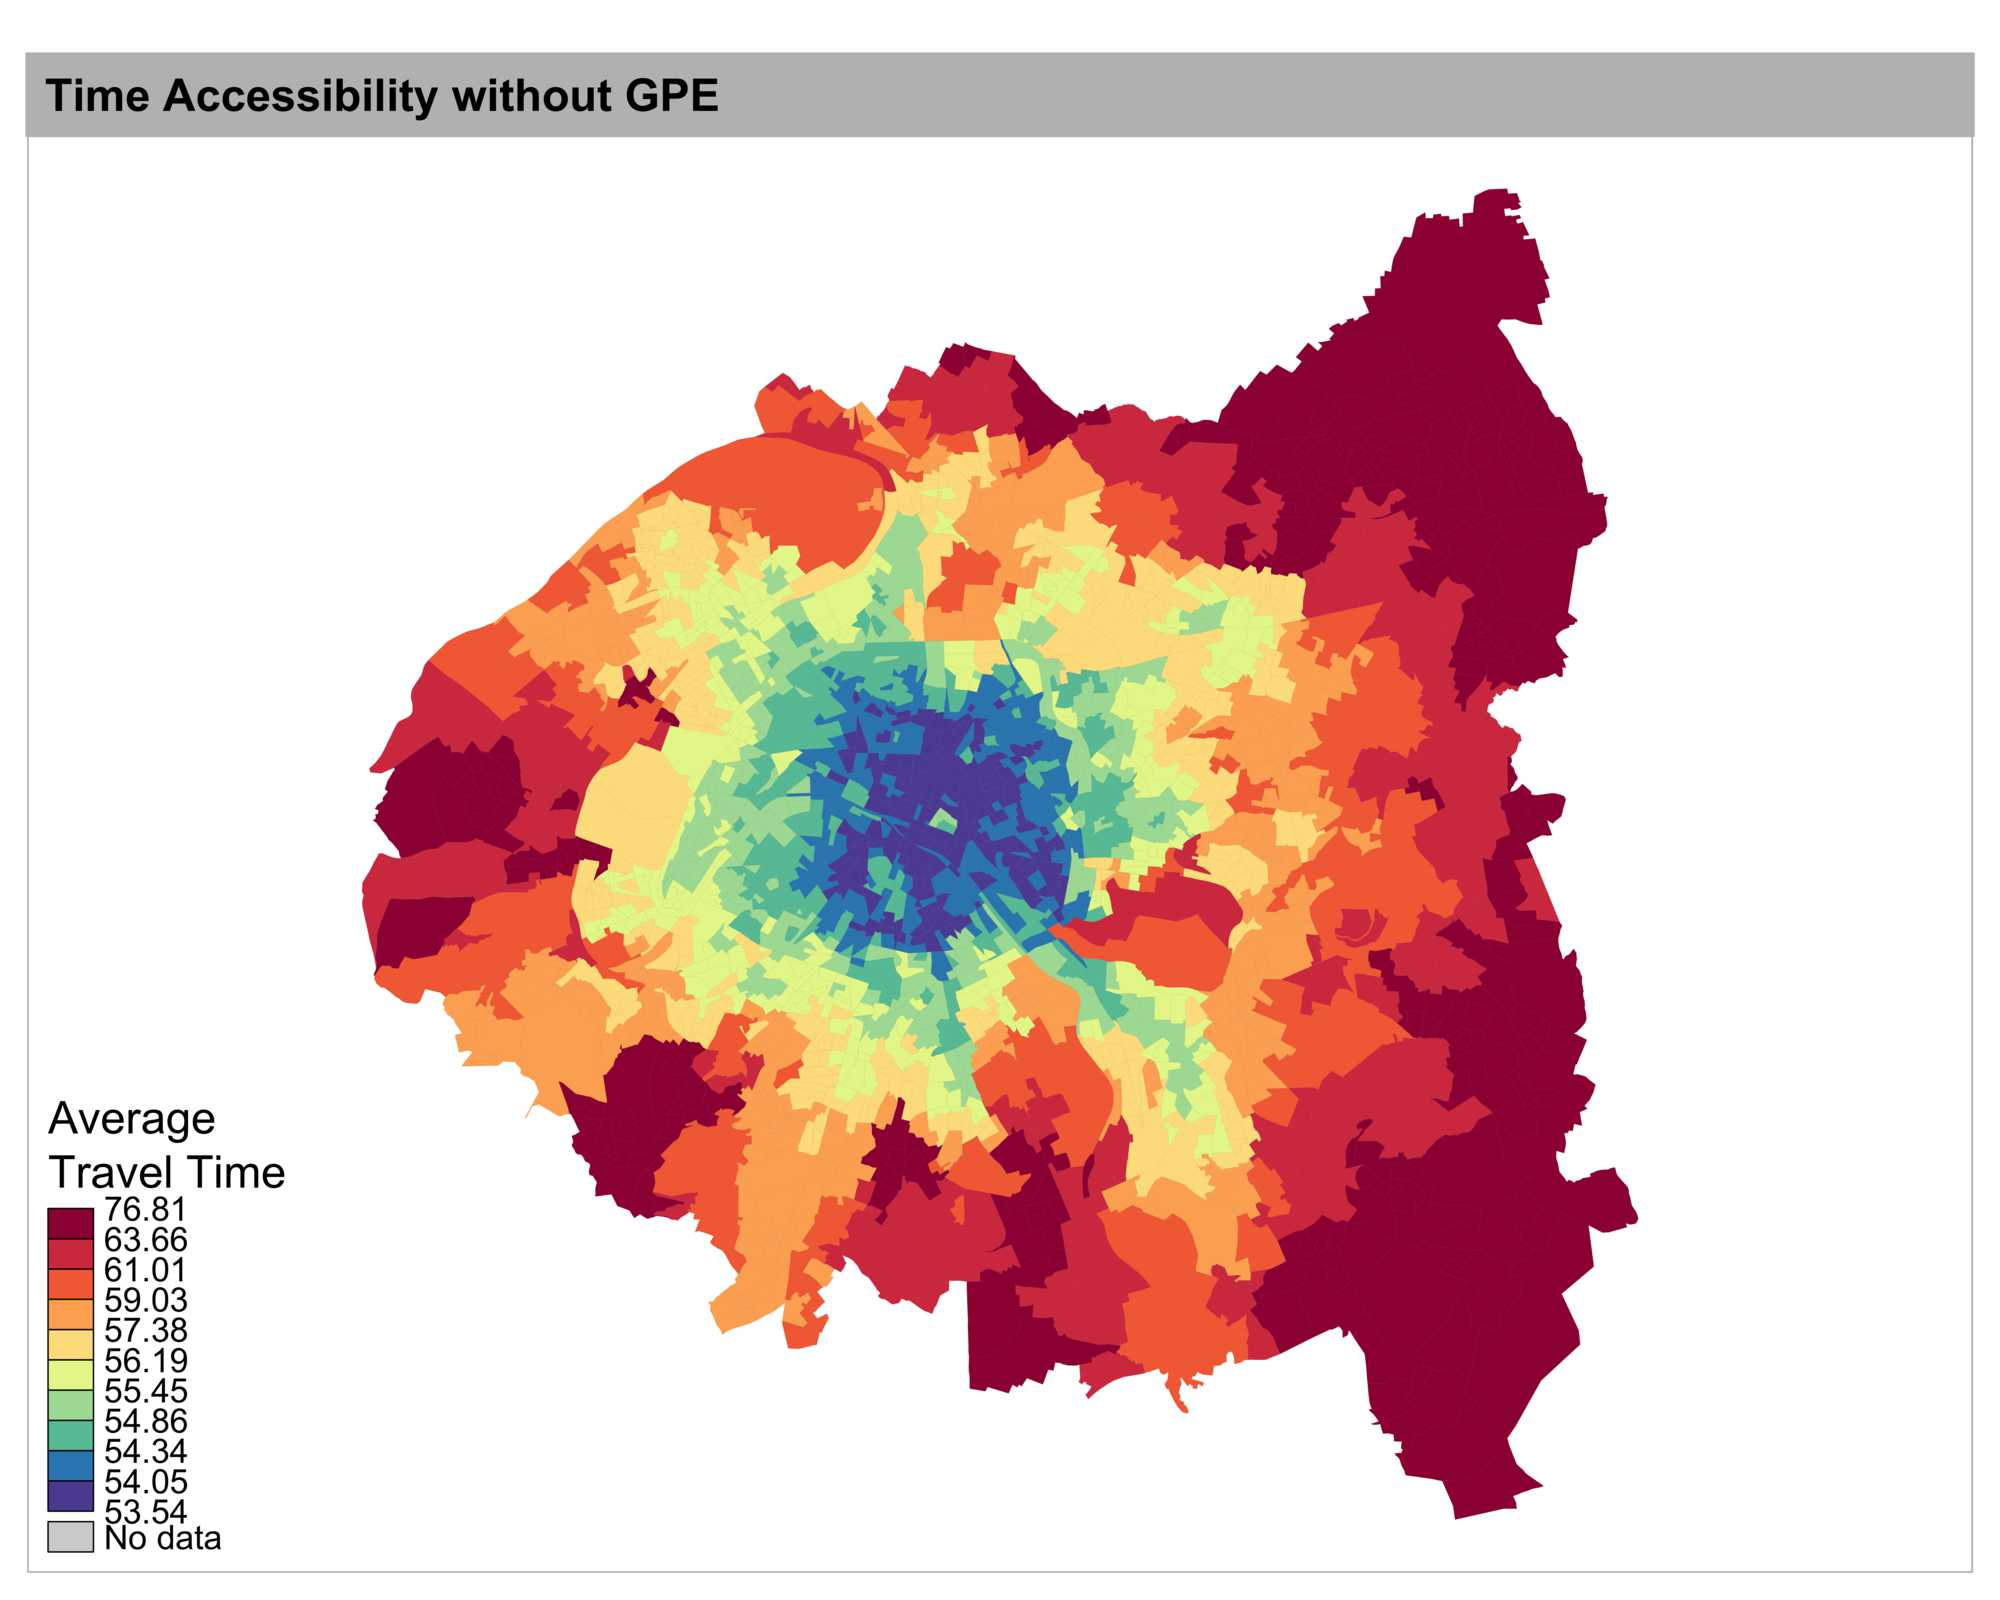
\includegraphics[width=0.8\linewidth]{Figures/CaseStudies/timeaccess_metropole}\\
	%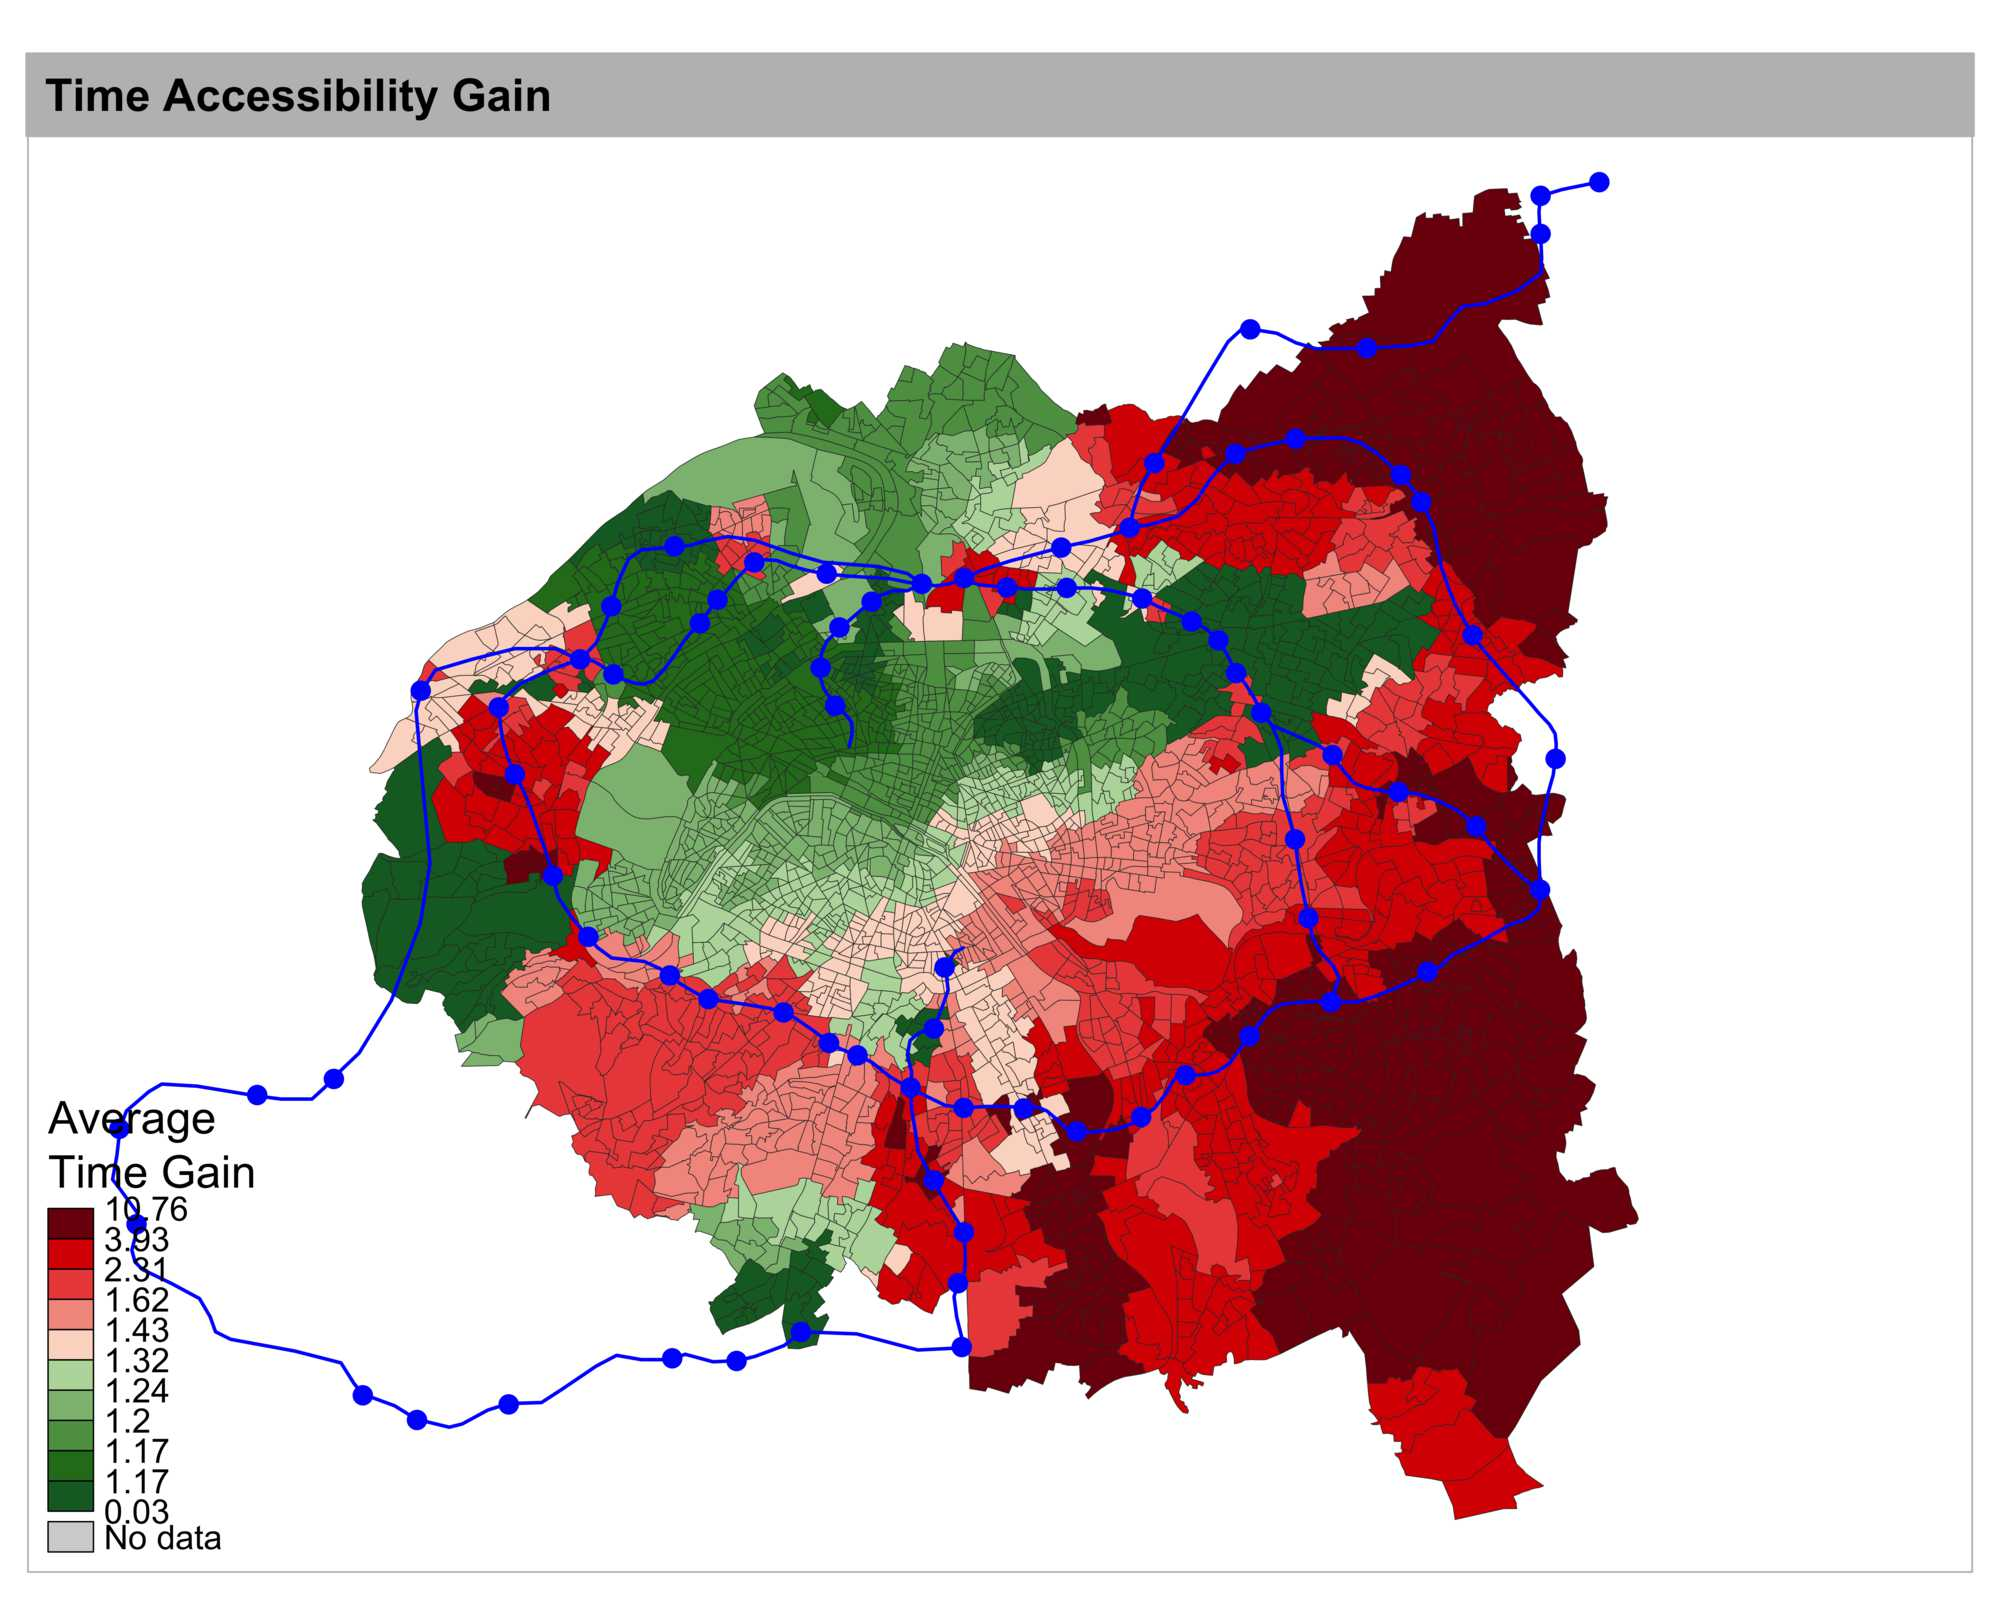
\includegraphics[width=0.8\linewidth]{Figures/CaseStudies/timegain_metropole}
	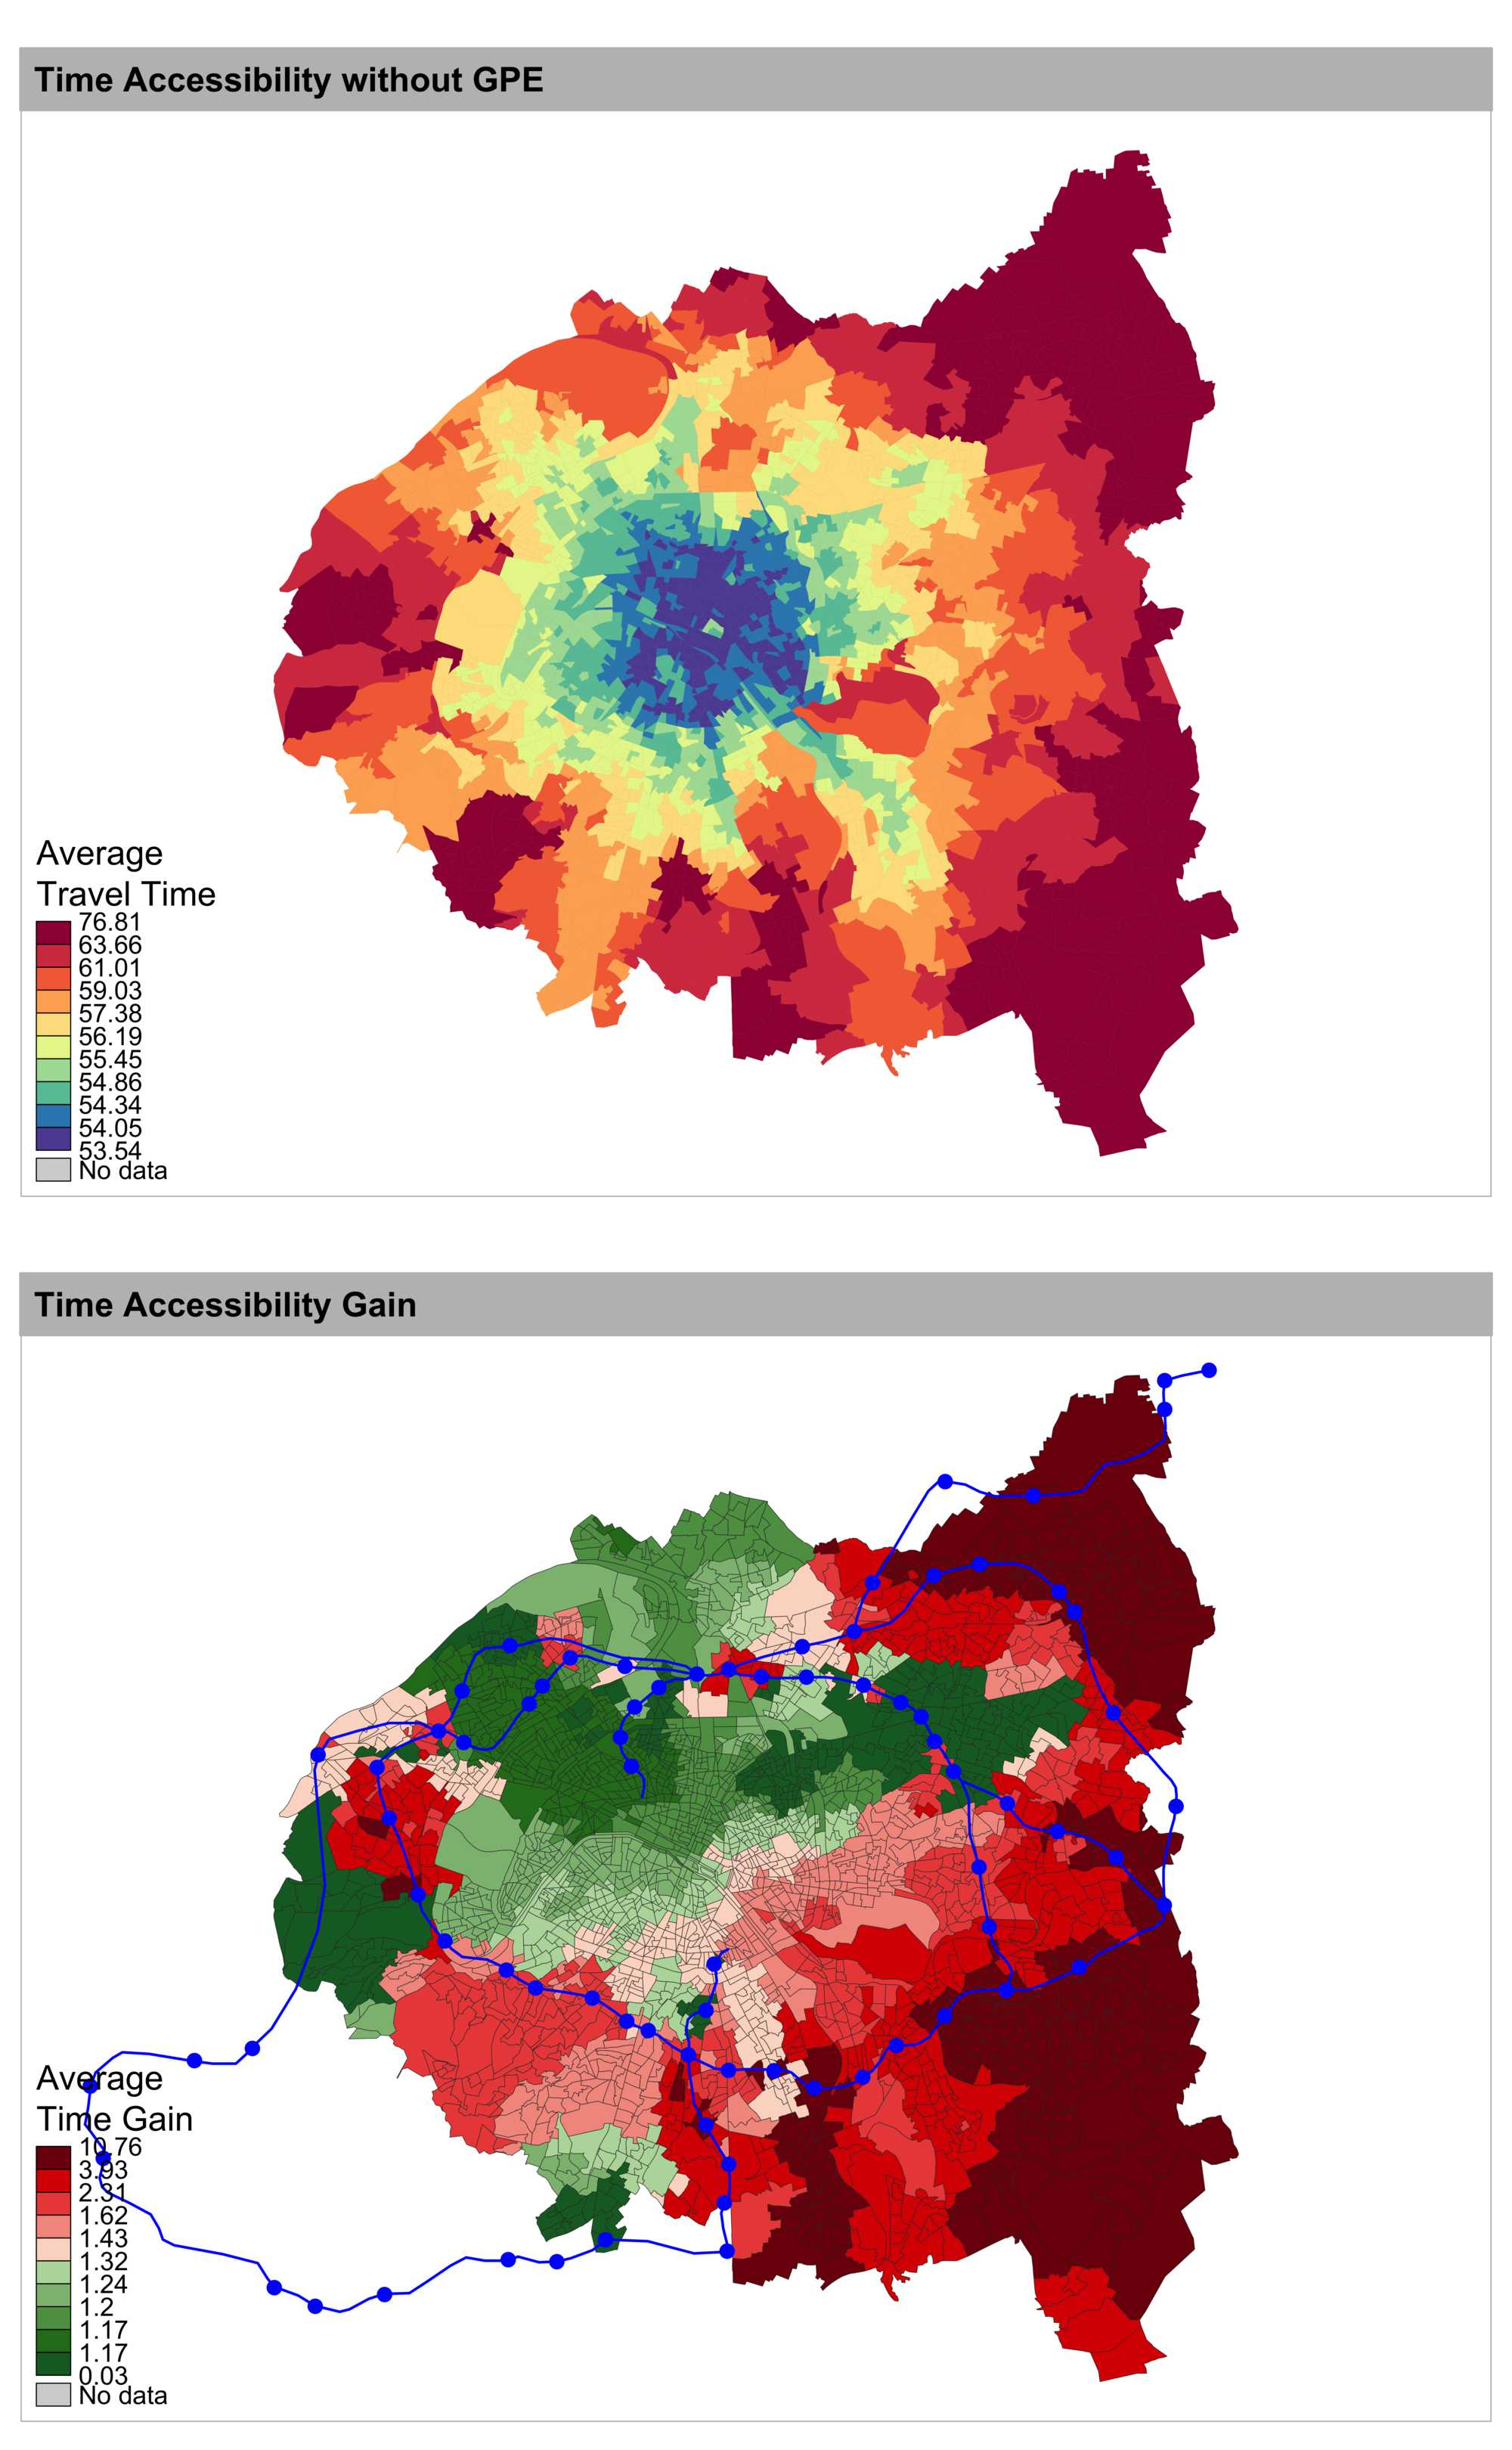
\includegraphics[width=\linewidth]{Figures/Final/1-2-1-fig-casestudies-gpe.jpg}
	\caption[Impact of \emph{Grand Paris Express}][Impact du Grand Paris Express]{\label{fig:casestudies:gpe}}{\textbf{Impact des lignes du GPE sur l'accessibilité temporelle.} \textit{(Haut)} Temps moyen de trajet vers l'ensemble des communes d'Ile-de-France, par transports en commun uniquement, pour les départements métropolitains ; \textit{(Bas)} Gains de temps permis par l'ensemble des lignes du GPE, avec le trajet des lignes.\label{fig:casestudies:gpe}\comment[AB]{traduire ; echelle monotone $\rightarrow$ gradient sur une gamme de couleurs}\comment[FL]{average time gain : entre quoi et quoi ? - gradation de couleurs discutable - pourquoi ces couleurs ? - sens ? ce n'est pas clair du tout - traduire ? que sont les zones ? par ailleurs tu n'as pas les contours de la metropole du grand paris - depuis Iris - communes.}}
\end{figure}
%%%%%%%%%%%%%%%%%%%




\bpar{
Various aspects of territories are concerned by interactions with networks. In previous empirical studies, no socio-economic attributes of populations inhabiting the territory nor economic values for land and real estate was considered. Both are however crucial elements of territorial dynamics and are extensively studied in fields such as territorial analysis or urban economics : for example, \cite{homocianu:tel-00359302} studies households residential choices to understand land-use transportation interactions. We propose here to use a database of Real Estate transactions for Parisian region on the last 20 years, with 2 years temporal granularity and exact spatial coordinates. \cite{guerois2009dynamique} used it to make typologies of spatial dynamics of Parisian real estate.
}{
Des aspects très variés des territoires sont concernés par l'interaction avec les réseaux. Dans nos études précédentes, les aspects économiques et financiers du foncier et l'immobilier n'ont pas été considérés. Il s'agit cependant d'éléments cruciaux des dynamiques territoriales et sont étudiés de manière intensive dans des champs comme l'analyse territoriale ou l'économie urbaine : par exemple, \cite{homocianu:tel-00359302} étudie les choix résidentiels des ménages pour comprendre les interactions entre usage du sol et transport. Nous proposons ici d'utiliser entre autres une base de données de transactions immobilières pour la région parisienne sur les 20 dernières années, avec une granularité temporelle de 2 ans et coordonnées spatiales exactes. \cite{guerois2009dynamique} l'utilise par exemple pour établir une typologie des dynamiques spatiales du marché immobilier parisien.
}


\bpar{
We propose to study the relations between accessibility differentials for each project, with variables linked to real estate and socio-economic variables. Indeed, the links between new lines and real estate value evolution are sometimes dramatic~\cite{damm1980response}. 
}
{
Cette étude plus précise peut être comprise comme une recherche de signes précurseurs de rupture de potentiels du réseau: en effet, si des dynamiques territoriales intrinsèques anticipent l'arrivée d'une nouvelle station de transports en commun, les implications seront bien différentes du cas où celle-ci conduit ces variables après sa construction. L'interprétation en termes ``d'effets structurants'' sera notamment très différente. Nous appliquons ici la méthode de causalités spatio-temporelles développée en~\ref{sec:causalityregimes}. Nous proposons d'étudier les relations entre différentiel d'accessibilité pour chaque projet, et variables liées au foncier (transactions immobilières) et socio-économiques. En effet, les liens entre nouvelles lignes et évolution du foncier sont parfois remarquables~\cite{damm1980response}.
}

\comment{sur les anticipations des acteurs : \cite{carrouet:hal-00980002} }


\cite{guerois2009dynamique} : bulles immobilières locales ?


\bpar{
Data for real estate transactions are contained within the BIENS database (\emph{Chambre des Notaires d'Ile de France}, proprietary database). The number of transactions that can be used after cleaning is 862360, distributed across all IRIS areas (basic census units in France), for a temporal span covering the years 2003 to 2012 included. The data at the IRIS level for population and income (median income and Gini index) come from INSEE. Network data have been vectorialized from projects maps (see figure~\ref{fig:projects} for the different projects). Travel times are computed by public transportation only, with standard values for average speeds of different modes (RER 60km.h\textsuperscript{-1}, Transilien 100km.h\textsuperscript{-1}, Metro 30km.h\textsuperscript{-1}, Tramway 20km.h\textsuperscript{-1}). The travel time matrix is computed from all the centroids of IRIS to all the centroids of \emph{Communes} (above aggregation level). These are linked to the network with abstract connectors to the closest station, with a speed of 50km.h\textsuperscript{-1} (travel by car). Analysis are implemented in R~\cite{rcoreteam} and all data, source code and results are available on an open git repository\footnote{At\\\texttt{https://github.com/JusteRaimbault/CityNetwork/tree/master/Models/SpatioTempCausality/GrandParis}. Data for the BIENS database are given only at the aggregated level of IRIS and for price and mortgage variables, for contractual reasons closing the database.}.
}{
Les données des transactions immobilières sont fournies par la base BIENS (Chambre des Notaires d'Ile de France, base propriétaire). Le nombre de transactions utilisables après nettoyage est de 862360, se répartissant sur l'ensemble des IRIS, pour une plage temporelle couvrant de 2003 à 2012 incluses. Les données par IRIS pour population et revenu (revenu médian et indice de Gini) proviennent de l'INSEE. Les données de réseau ont été vectorialisées à partir des cartes des projets (voir Fig.~\ref{fig:projects} pour les projets). Les temps de trajets sont calculés par transport en commun uniquement, avec des valeurs standard pour les vitesses moyennes des différents modes (RER 60km.h\textsuperscript{-1}, Transilien 100km.h\textsuperscript{-1}, Metro 30km.h\textsuperscript{-1}, Tramway 20km.h\textsuperscript{-1}). La matrice des temps est calculée depuis l'ensemble des centroïdes des IRIS vers l'ensemble des centroïdes des communes. Ceux-ci sont reliés au réseau par des connecteurs à la gare la plus proche, de vitesse 50km.h\textsuperscript{-1} (trajet en voiture). Les analyses sont implémentées intégralement en langage R~\cite{rcoreteam} et l'ensemble des données, du code source et des résulats sont disponibles sur un dépôt git ouvert\footnote{A l'adresse\\\texttt{https://github.com/JusteRaimbault/CityNetwork/tree/master/Models/SpatioTempCausality/GrandParis}. Les données de la base BIENS ne sont fournies que de manière agrégée à l'IRIS et pour les variables de prix et de crédit, pour des raisons de fermeture contractuelle de la base brute.}.
}



%%%%%%%%%%%%%%%
\begin{figure}
%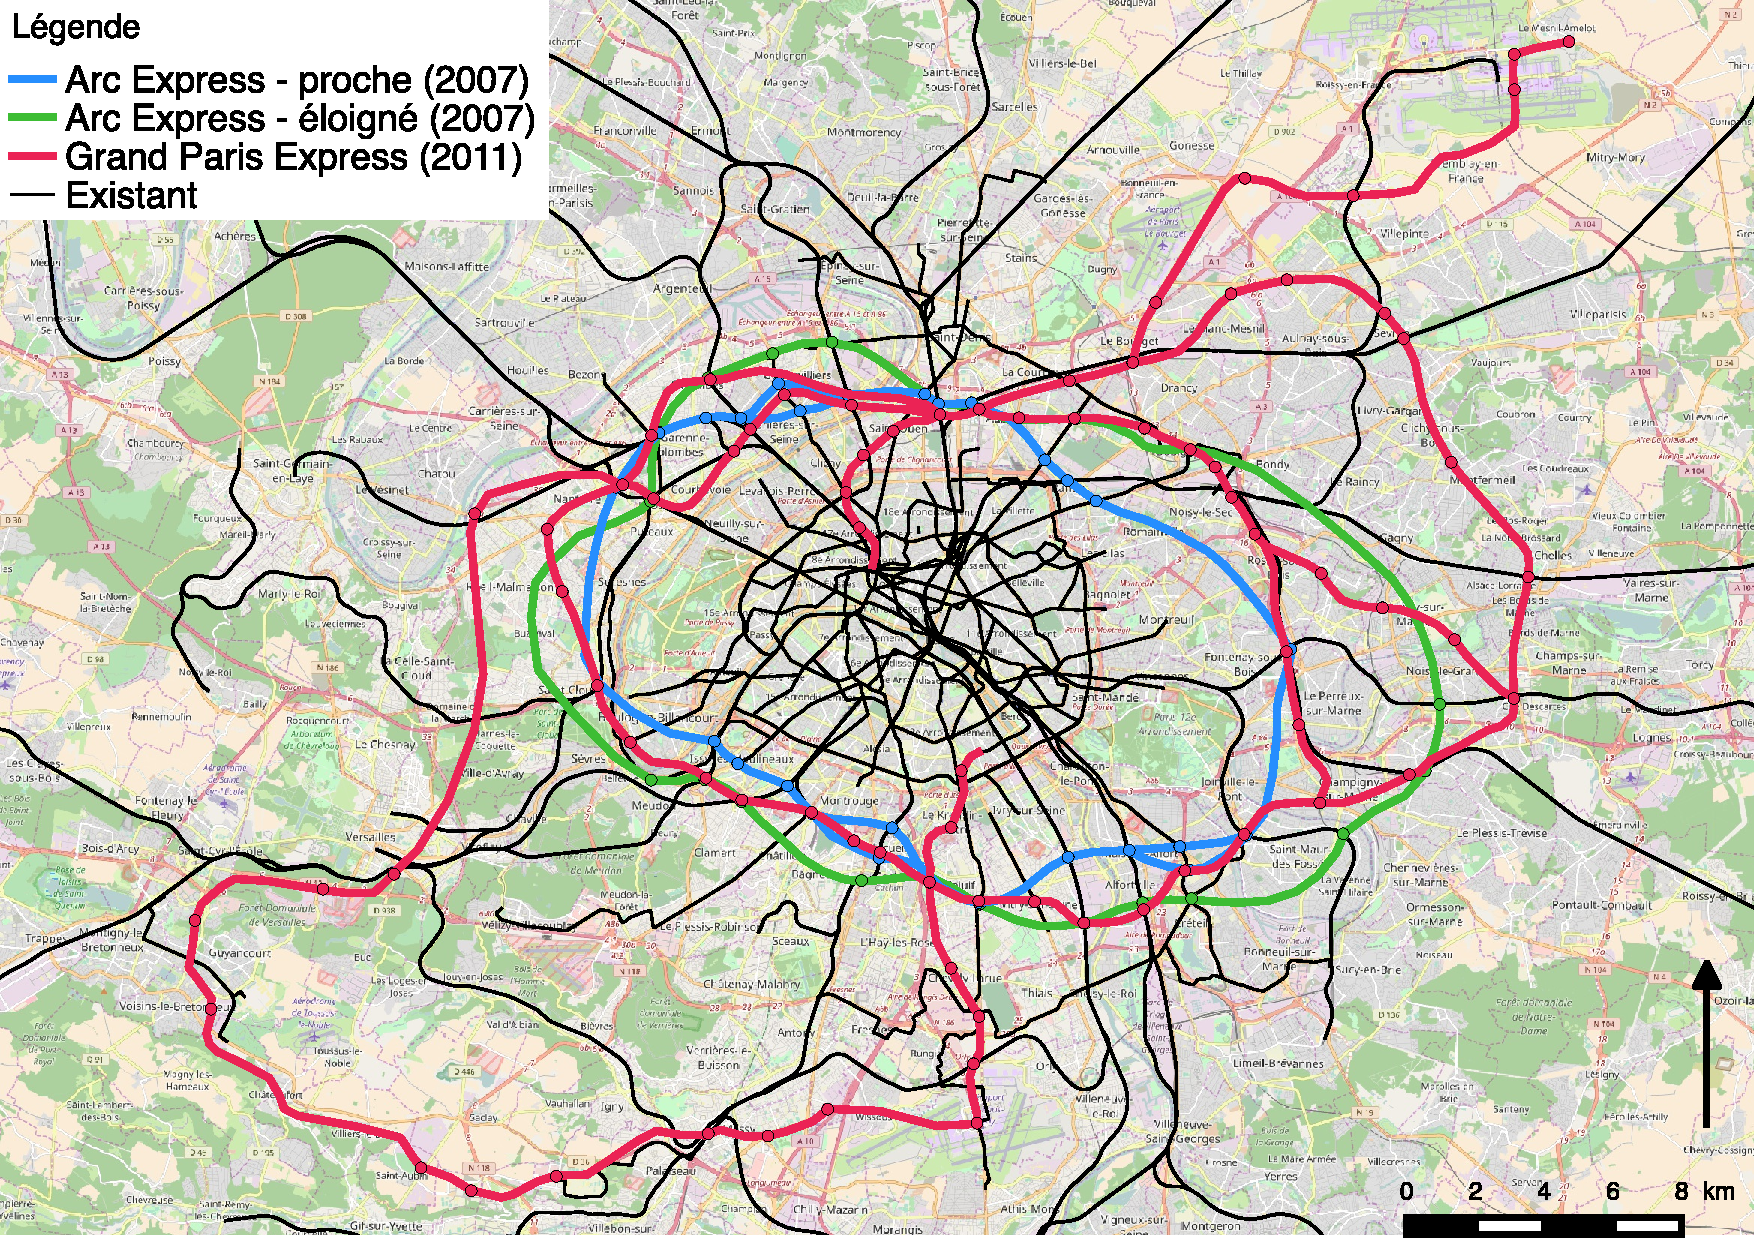
\includegraphics[width=\linewidth]{Figures/GrandParisRealEstate/reseaux}
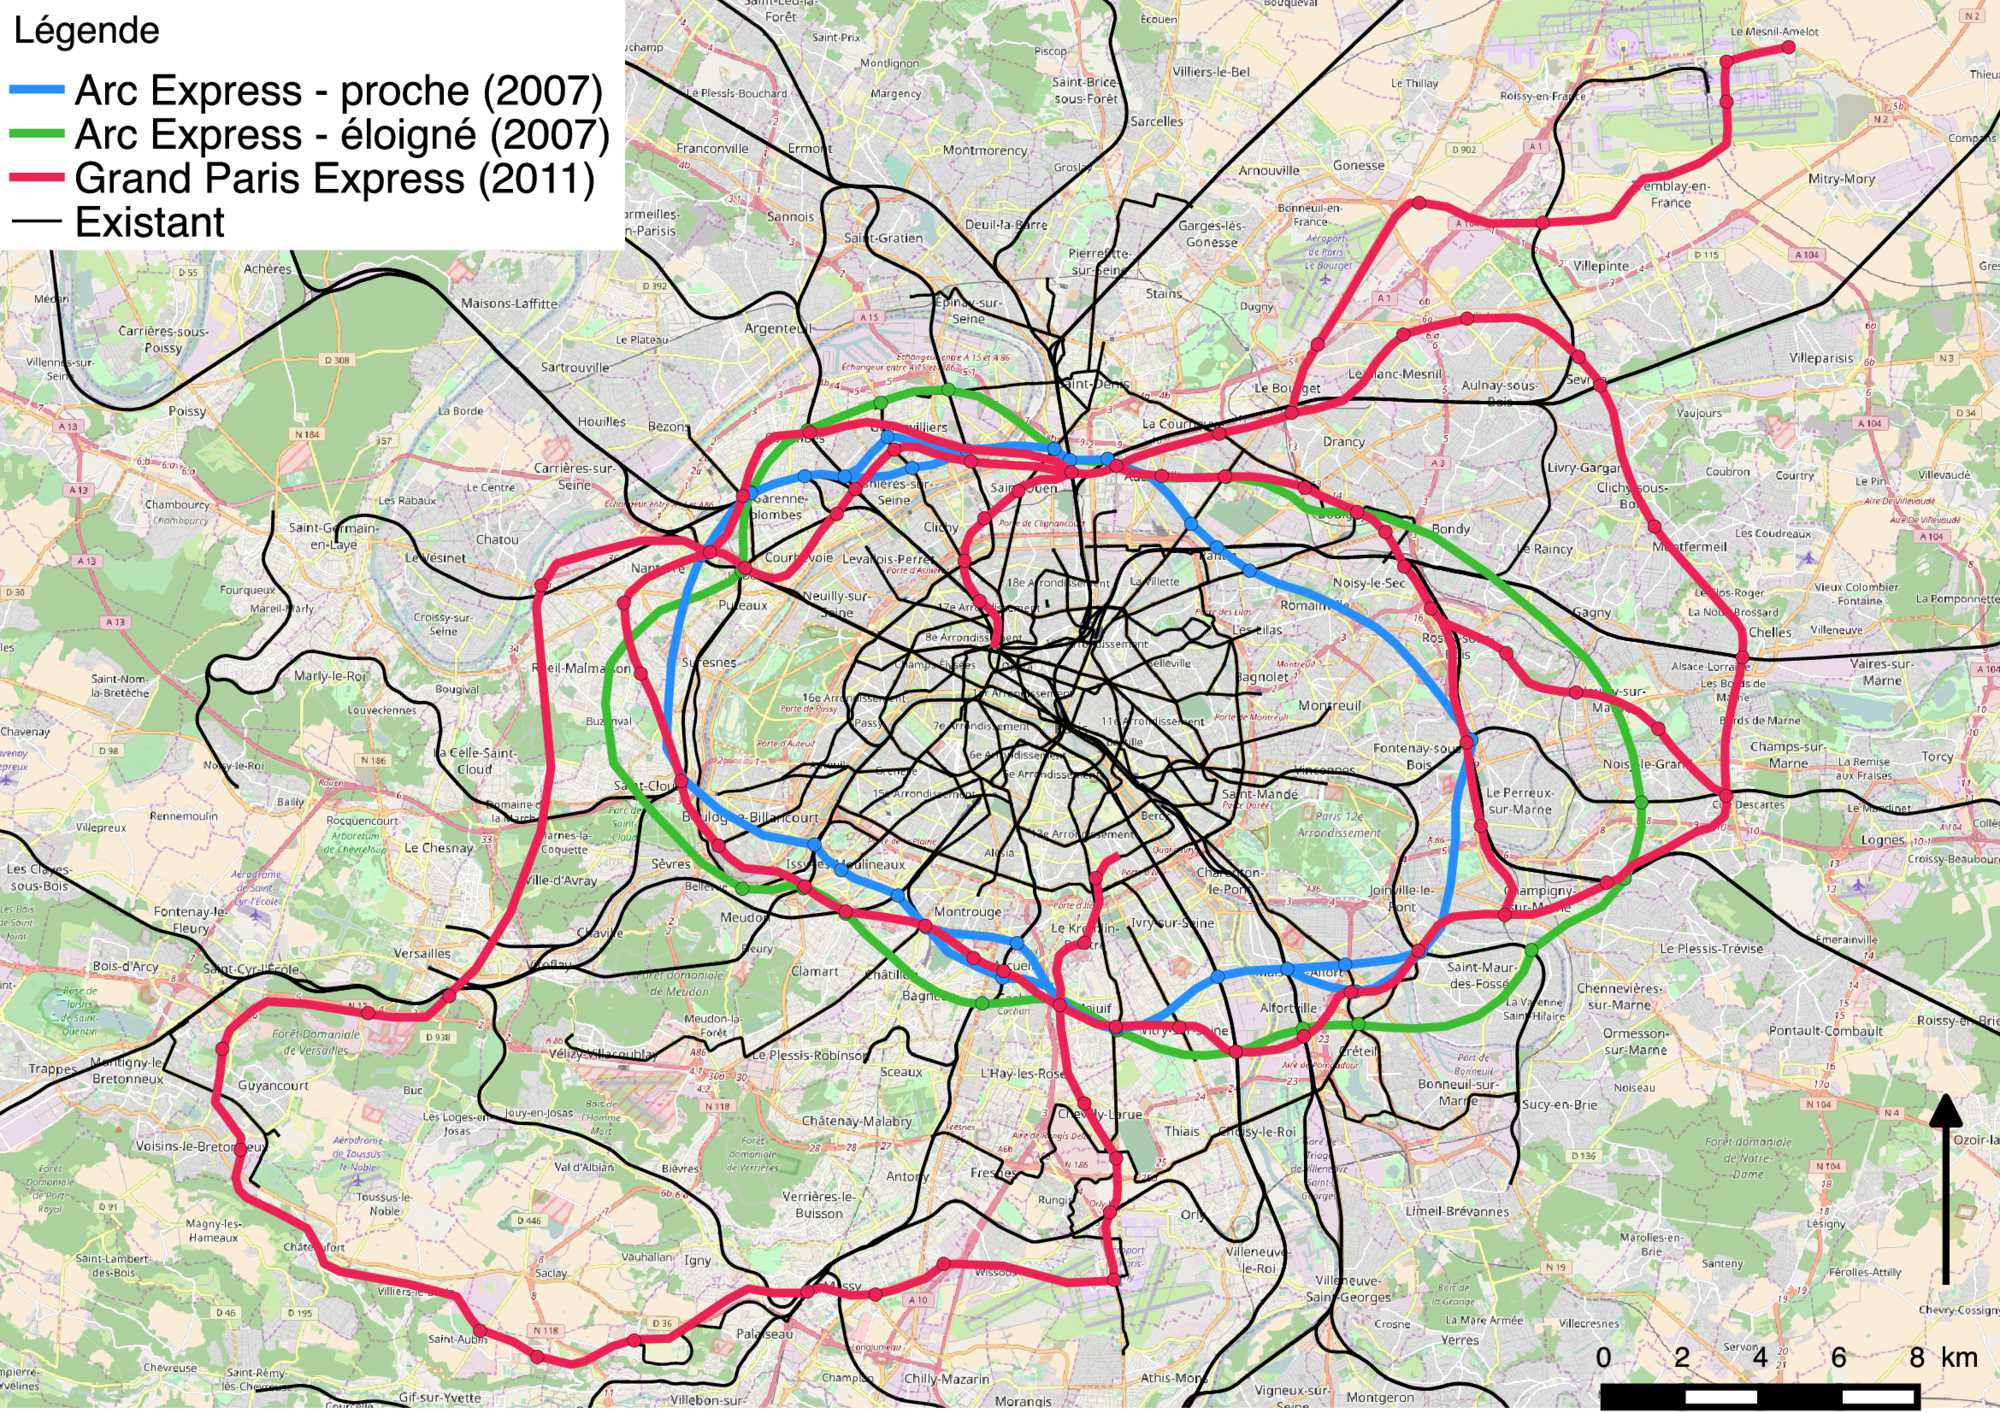
\includegraphics[width=\textwidth]{Figures/Final/1-2-1-fig-casestudies-projects.jpg}
\caption[][Projets de transport successifs du Grand Paris]{\textbf{Successive transportation network projects for the Grand Paris metropolitan area.} We show the two alternatives for the \emph{Arc Express} project elaborated by the Region, and the \emph{Grand Paris Express} (GPE) advocated by the State. The \emph{Réseau du Grand Paris}, a precursor for GPE, is not shown here for visibility reasons because of its proximity with it.\label{fig:projects}}{\textbf{Projets de transport successifs de la métropole du Grand Paris.} Nous montrons les deux alternatives du projet Arc Express porté par la région, et le Grand Paris Express (GPE) porté par l'état. Le Réseau du Grand Paris, précurseur du GPE, n'est pas montré ici pour des raisons de visibilité à cause de sa proximité avec celui-ci.\label{fig:casestudies:projects}}
\end{figure}
%%%%%%%%%%%%%%%


\bpar{

We compute for each project accessibility differentials $\Delta T_i$ in average travel time from each IRIS, in comparison with the network without the project. Average travel time accessibility is defined as $T_i = \sum_k \exp{-t_{ik}/t_0}$ with $k$ \emph{Communes}, $t_{ik}$ travek time, and $t_0$ a decay parameter. To each project is associated a date\footnote{2006 for \emph{Arc Express}, 2008 for \emph{Réseau du Grand Paris} and 2010 for \emph{Grand Paris Express}}, corresponding roughly to the mature announcement of the project. It stays a bit arbitrary as it is difficult on the one hand to determine precisely as a planning project does not emerge from nothing in one day, and one the other hand it may correspond to different realities of learning about the project by economic agents (we do therefore the limiting but necessary assumption of a diffusion of information for the majority of agents in a time smaller than a year). We study the lagged correlations of this variable with the variations $\Delta Y_{ij}$ of the following socio-economic variables: population, median income, Gini index for income, average price of real estate transactions and average value of real estate mortgages. A Fisher test is done for each estimation and the value is set to 0 if it is not significant ($p<0.05$ in a classical manner). The study with generalized accessibility in the sense of Hansen has also been conducted but is less interesting as it has a very low sensitivity to the mobility component (network and decay) compared to the variables themselves. It informs therefore only on relations between these and is not presented here.
}{
Nous calculons pour chaque projet, le différentiel $\Delta T_i$ d'accessibilité en temps moyen de trajet à partir de chaque IRIS en comparaison à celui dans le réseau sans le projet, défini par $T_i = \sum_k \exp{-t_{ik}/t_0}$ avec $k$ communes, $t_{ik}$ temps de trajet, et $t_0$ paramètre d'atténuation. A chaque projet est associée une date\footnote{2006 pour Arc Express, 2008 pour le Réseau du Grand Paris, 2010 pour le Grand Paris Express}, correspondant environ à l'année d'annonce mature du projet, restant toutefois arbitraire car difficile d'une part à déterminer précisément, un projet n'émergeant pas d'un coup du jour au lendemain, et d'autre part pouvant correspondre à des réalités différentes d'apprentissage du projet par les différents agents économiques (nous faisons donc l'hypothèse réductrice mais nécessaire d'une diffusion sur la majorité des agents dans un temps inférieur à l'année). Nous étudions les corrélations décalées de cette variable avec les variations $\Delta Y_{ij}$ des variables socio-économiques suivantes : population, revenu médian, indice de Gini des revenus, prix moyen des transactions immobilières et montant moyen des crédits immobiliers. Un test de Fisher est effectué pour chaque estimation, et la valeur est fixée nulle si celui-ci n'est pas significatif ($p<0.05$ de manière classique). L'étude avec accessibilité généralisées au sens de Hansen a également été menée mais moins intéressante car très peu sensible à la composante mobilité (réseau et atténuation) par rapport aux variables elle-même, informe uniquement sur des relations entre celles-ci et n'est donc pas présentée ici.
}


\bpar{
We show in figure~\ref{fig:empiricalres} the results for all networks and variables. It is first remarkable to note the presence of significant effects for all variables. Lower values for the parameter $t_0$ give correlations higher in absolute value, unveiling a possible higher importance of local accessibility on territorial dynamics. The behavior of population shows a clearly detached peak corresponding to 2008, what suggests an impact of the older project \emph{Arc Express} on population growth, the effect of other projects would then be spurious from their proximity in the most important branches. It would imply that areas where they are fundamentally different such as \emph{Plateau de Saclay} are less sensitive to transportation projects, what would confirm the artificial planned aspect of the development of this territory. Concerning income, we observe a similar behavior but in a negative way, what would imply a decrease of wealth linked to the increase of accessibility, however accompanied by a decrease of inequalities. Finally, real estate prices are as expected driven by the potential arrival of new networks. This effect disappear after two years for the \emph{Grand Paris Express}, suggesting a temporal speculation bubble. We demonstrate thus the existence of complex lagged correlation links, that we call causalities in this sense, between territorial dynamics and anticipated dynamics of networks. A finer understanding of working processes is beyond the scope of this paper and would imply for example qualitative fieldwork or targeted case studies. This example shows however the operational potentialities of our method on a real case study.

}{
Nous présentons en Fig.~\ref{fig:empiricalres} les résultats pour l'ensemble des réseaux et variables. Il est remarquable tout d'abord de noter l'existence d'effets significatifs pour l'ensemble des variables. Des valeurs plus basses du paramètre $t_0$ donnent des corrélations plus fortes en valeur absolue, révélant une possible plus grande importance de l'accessibilité locale sur les dynamiques territoriales. Le comportement de la population montre un pic très détaché correspondant à 2008, laissant supposer un impact du plus vieux projet d'Arc Express sur la croissance de la population, l'effet des autres projets serait alors fallacieux de par leur proximité dans les grands tronçons : cela impliquerait que les zones où ils diffèrent fondamentalement comme le Plateau de Saclay ne soient que très peu sensibles au projet de transport, ce qui confirmerait l'aspect artificiel planifié du développement de ce territoire. Concernant les revenus, on observe un comportement similaire mais négatif, ce qui impliquerait un appauvrissement lié à l'augmentation de l'accessibilité, mais qui semble toutefois s'accompagner d'une baisse des inégalités. Enfin, comme attendu les prix immobiliers sont tirés par l'arrivée potentielle des nouveaux réseaux, effet qui disparait à deux ans pour le Grand Paris Express, suggérant une bulle immobilière passagère. Nous démontrons ainsi l'existence de liens de correlations retardées complexes qu'on nomme causalités en ce sens, entre dynamiques territoriales et dynamiques anticipées des réseaux. Une compréhension plus fine des processus à l'oeuvre est au delà de la portée de cet article, car supposerait des études de terrain qualitatives, des études de cas ciblées, etc. Cet exemple illustre cependant le caractère opérationnel de notre méthode sur un cas d'étude réel.
}




%%%%%%%%%%%%%%%
\begin{figure}[h!]
%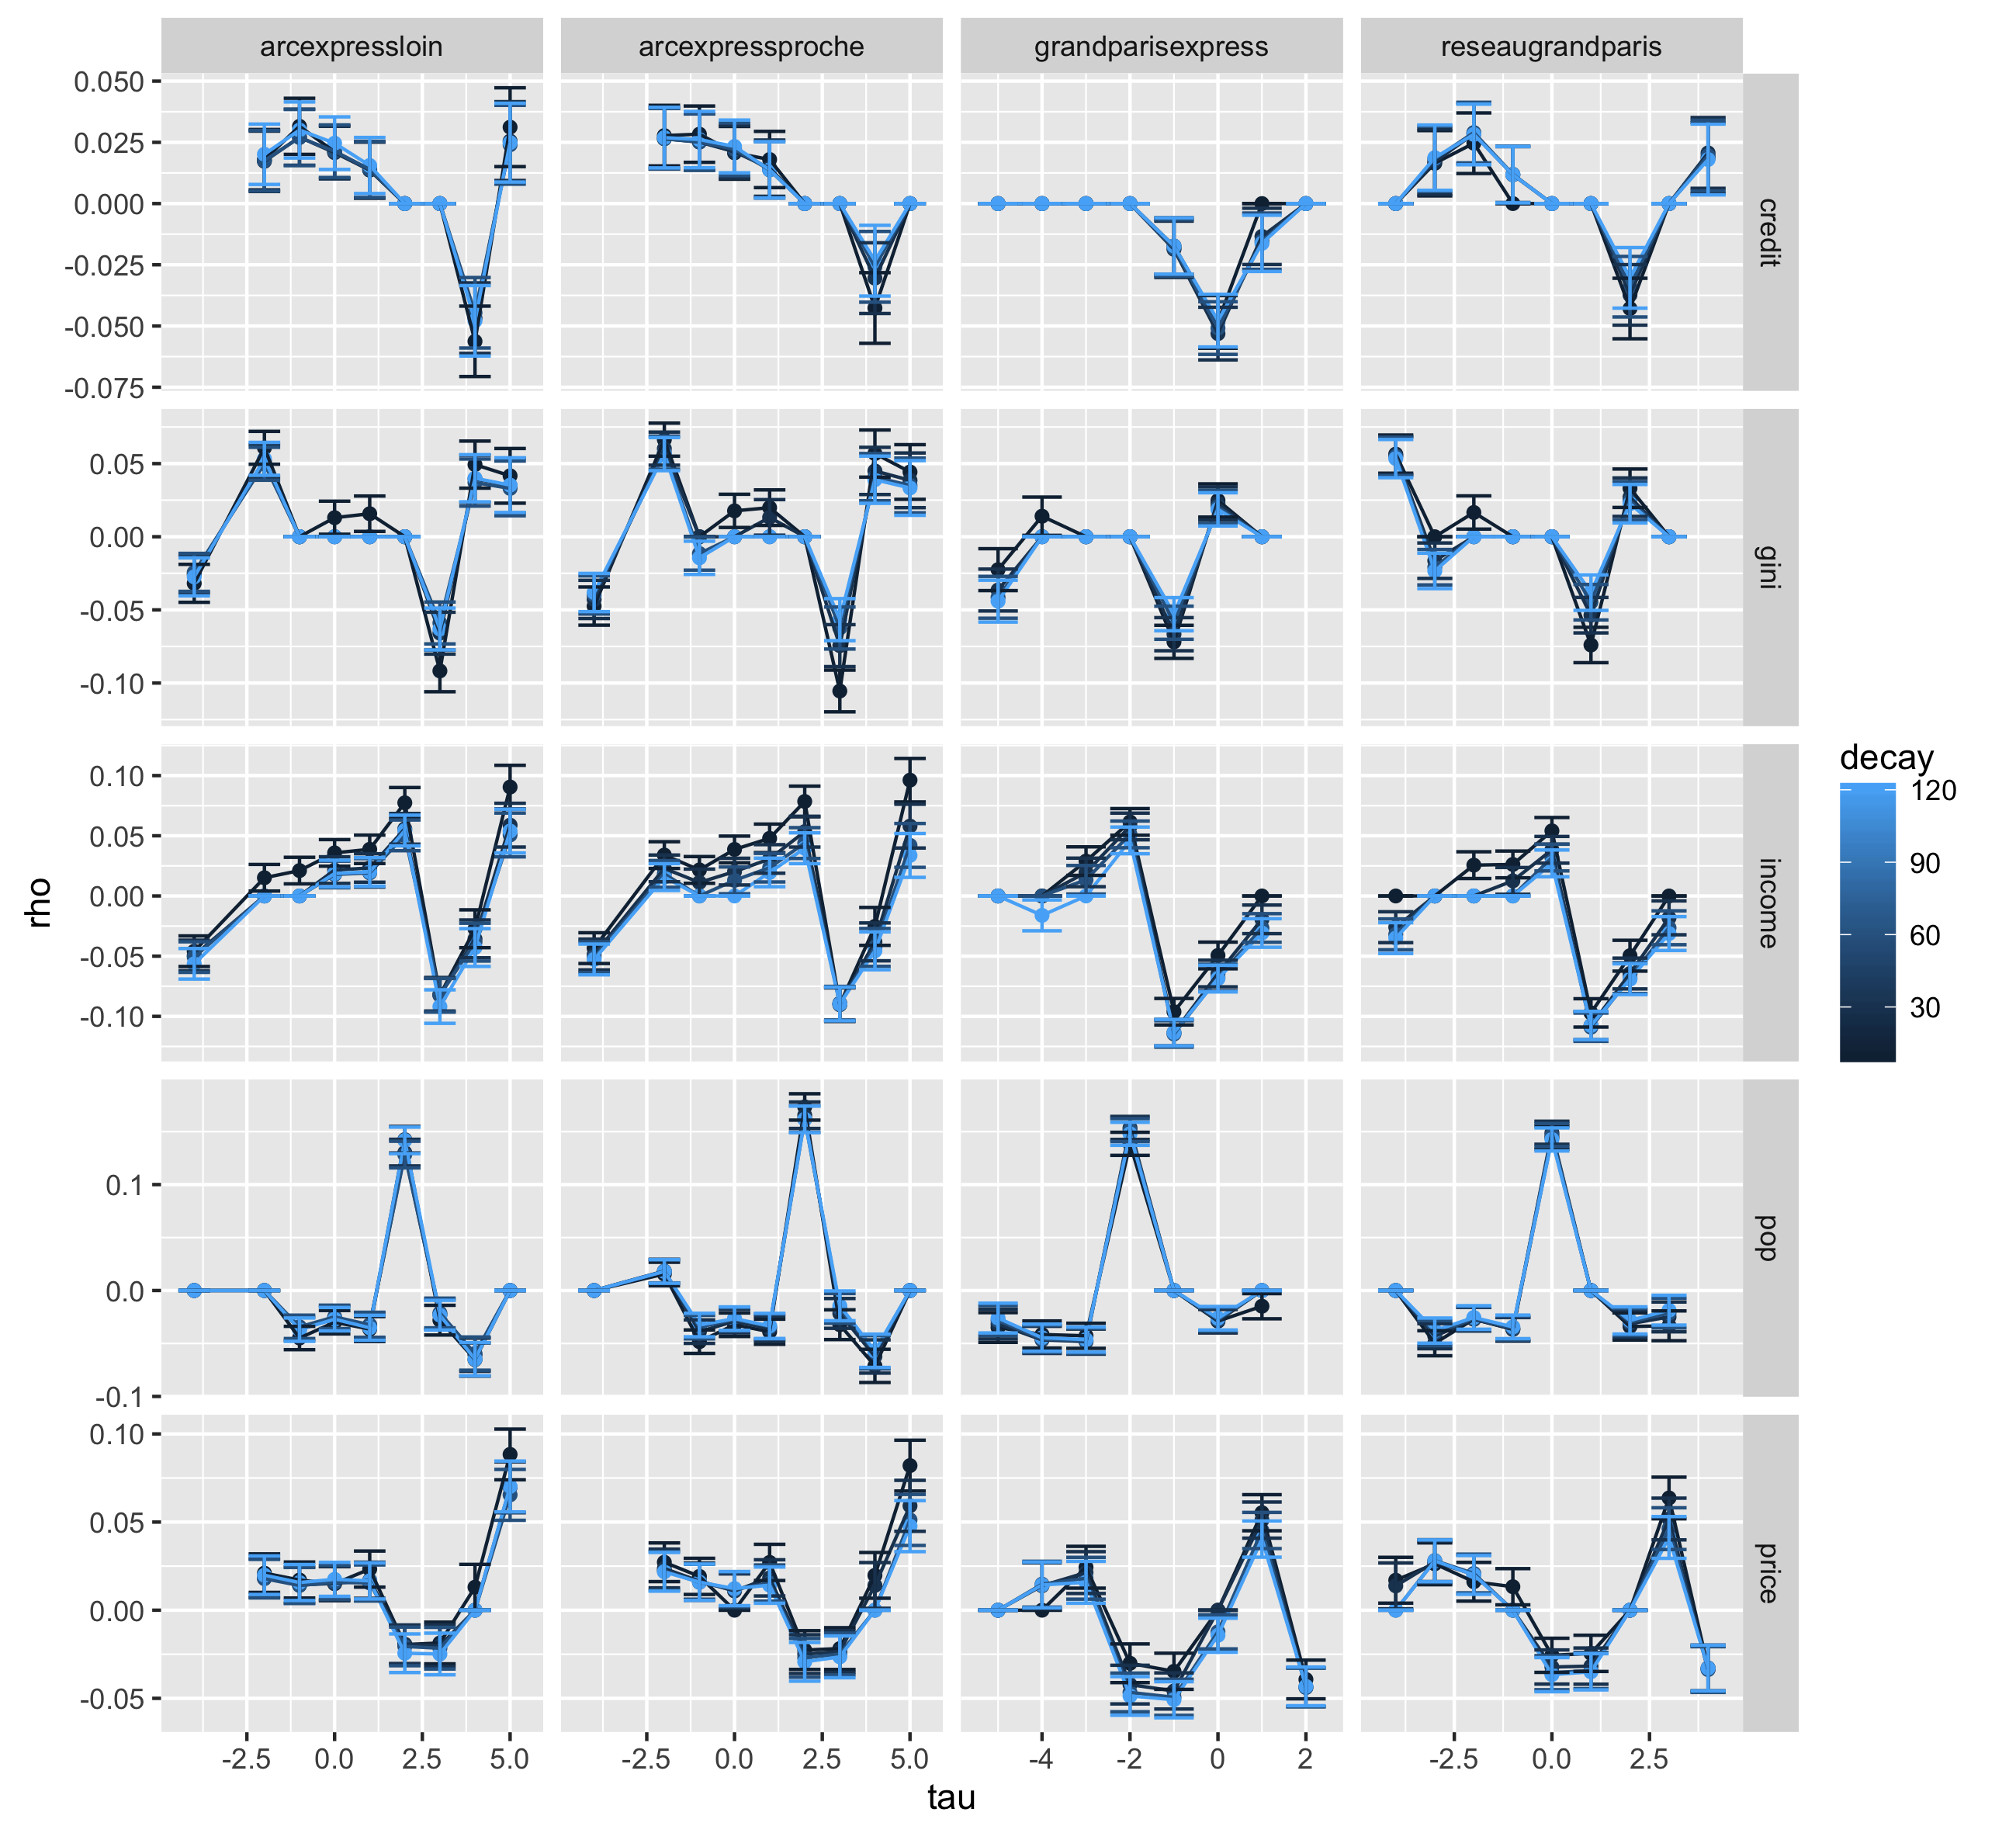
\includegraphics[width=\linewidth]{Figures/GrandParisRealEstate/laggedcorrs_times_allvars}
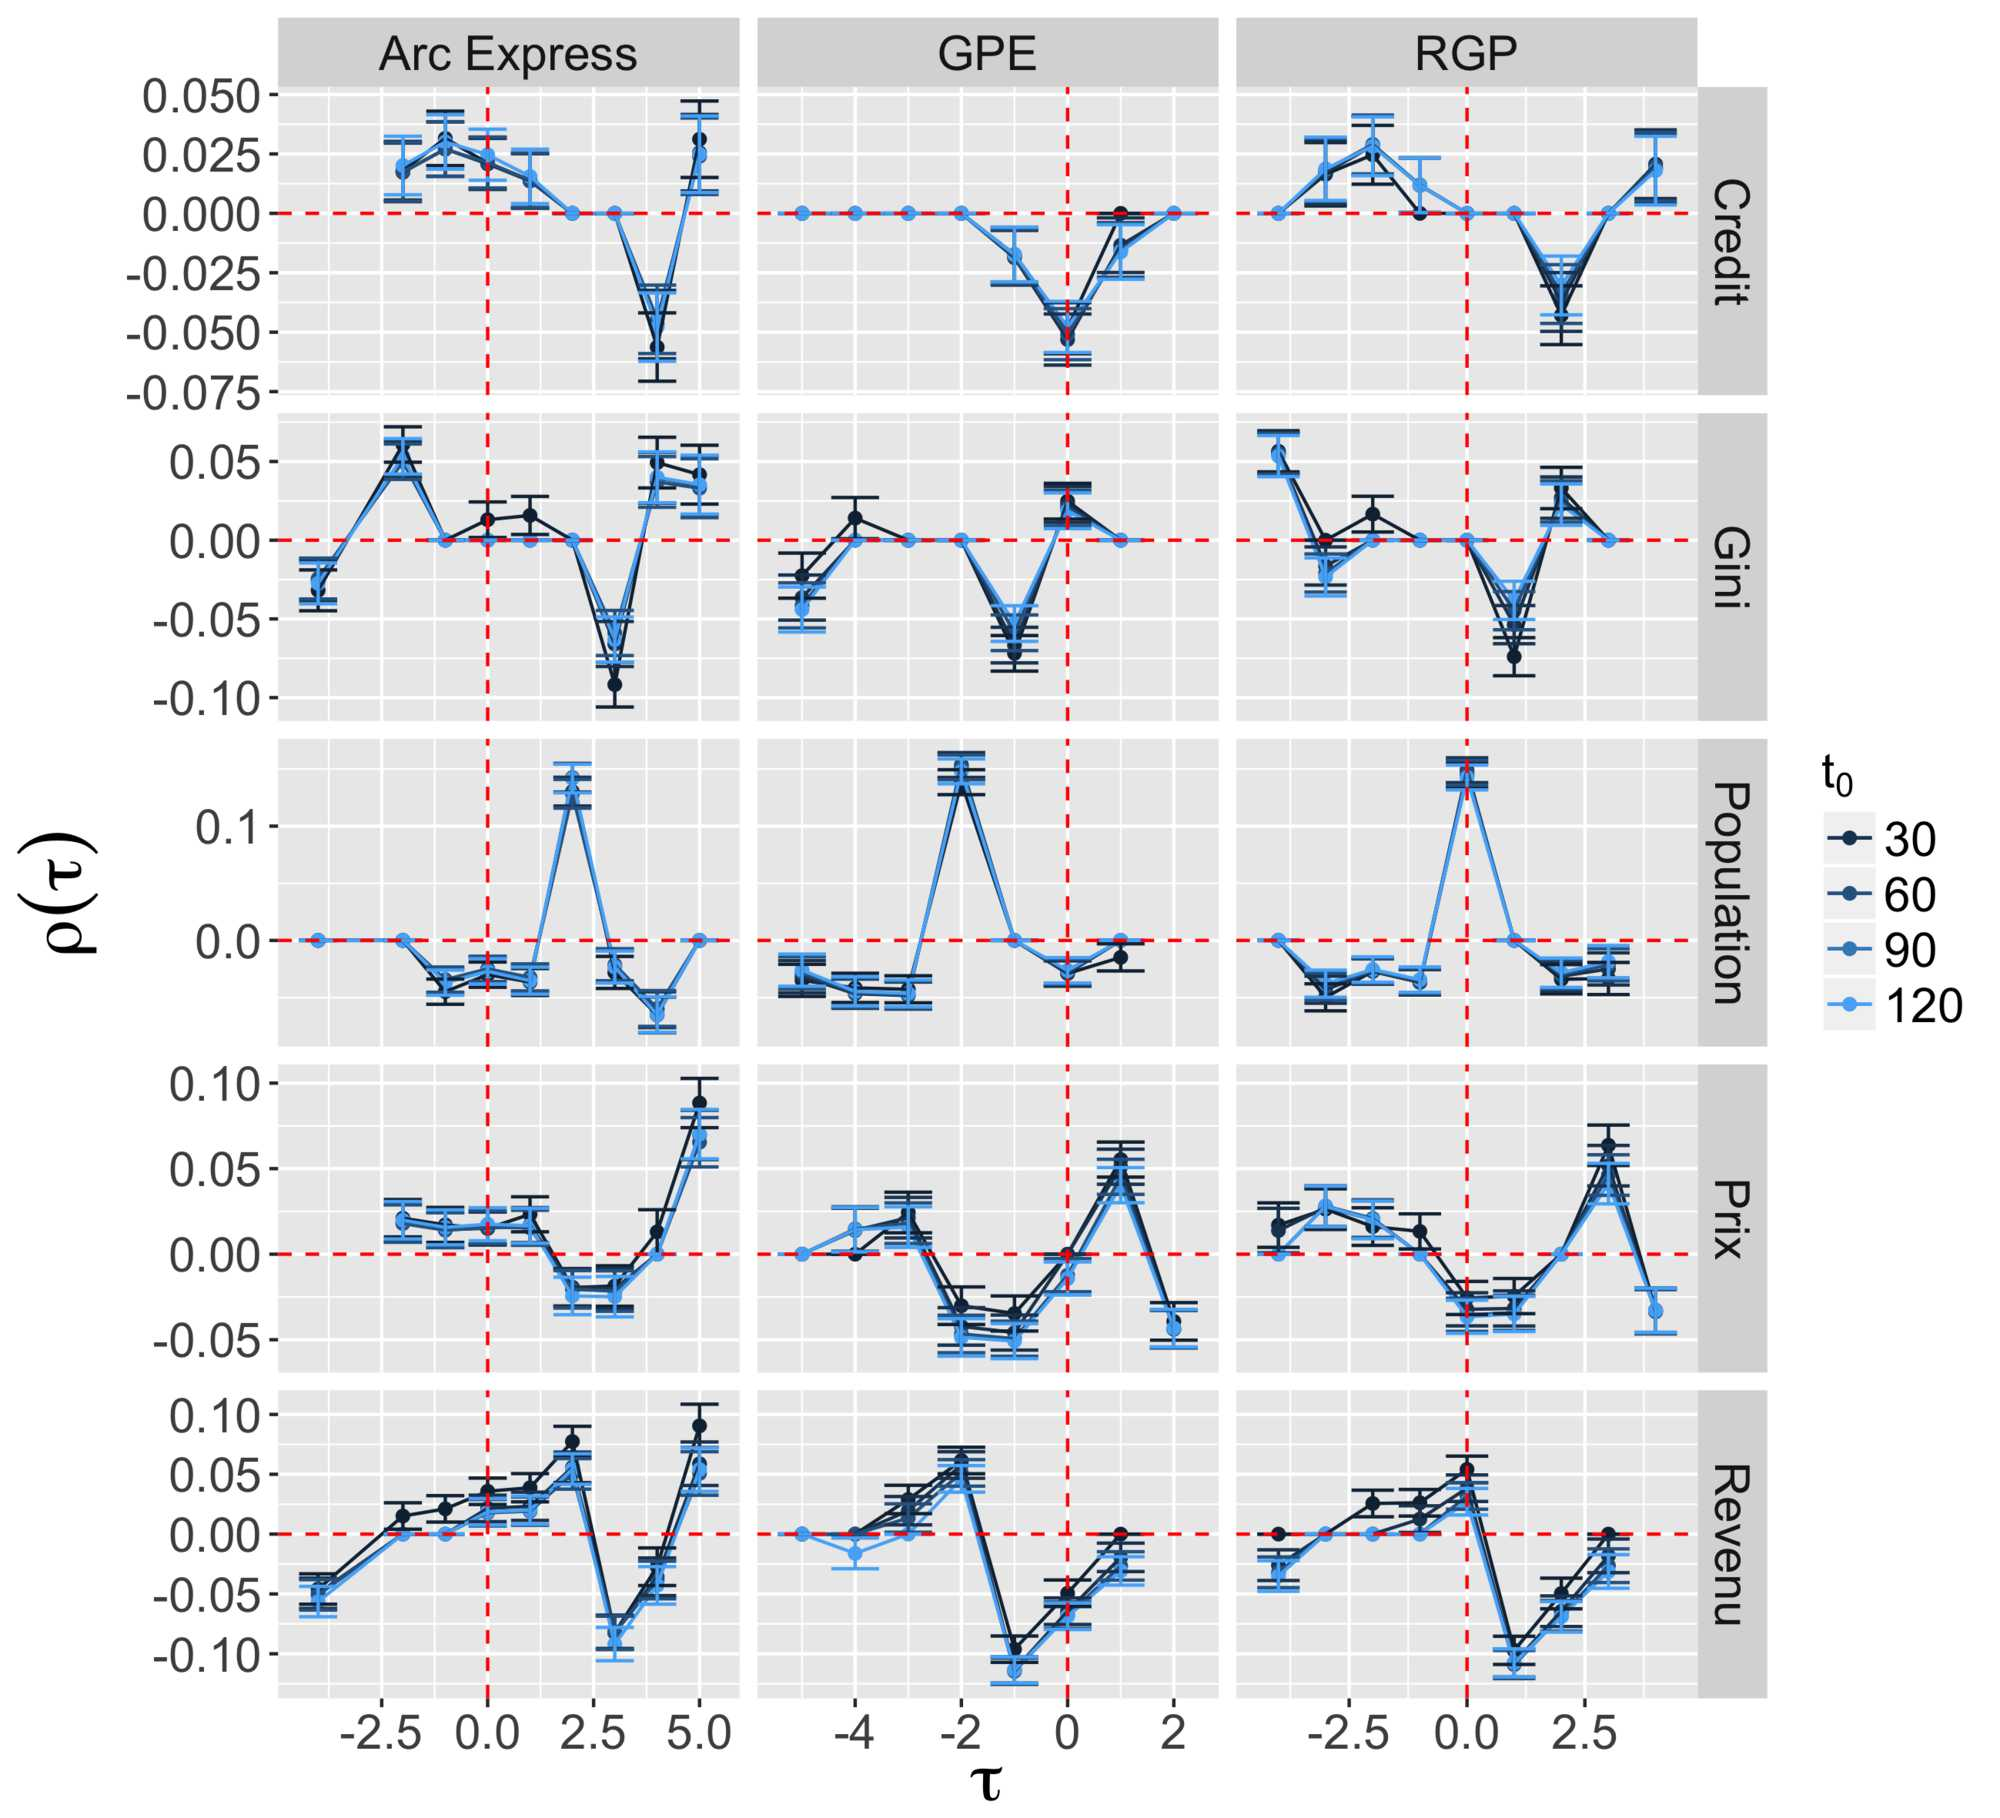
\includegraphics[width=\linewidth]{Figures/Final/1-2-1-fig-casestudies-empiricalres.jpg}
\caption[][Corrélations retardées empiriques]{\textbf{Empirical lagged correlations.} Plots show the value of lagged correlation between accessibility differentials in average travel time $\Delta T$ for each project (in colunms) and socio-economic and real estate variables variations (in rows). All are computed for different values of the decay parameter (\texttt{decay}, given by curve color). Error bars give the 95\% confidence interval.\label{fig:empiricalres}}{\textbf{Corrélations retardées empiriques.} Les graphiques donnent la valeur de la correlation entre le différentiel d'accessibilité en temps de trajet moyen $\Delta T$ pour chaque projet (en colonnes) et le différentiel des différentes variables socio-economiques et de transactions immobilières (en lignes), pour différentes valeurs du paramètre d'atténuation (\texttt{decay}). Les barres d'erreur donnent l'intervalle de confiance à 95\%.\label{fig:casestudies:empiricalres}}
\end{figure}
%%%%%%%%%%%%%%%
















%-------------------------


%%%%%%%%%%%%%%%%%%%%%%%%
%\subsection[Pearl River Delta][Le Delta de la Rivière des Perles]{Pearl River Delta: new urban regimes and mega-city regions}{Le Delta de la Rivière des Perles : nouveaux régimes urbains et Mega-région urbaine}
\subsection{Pearl River Delta}{Le Delta de la Rivière des Perles}


\paragraph{New urban regimes and mega-city regions}{Nouveaux \emph{régimes urbains} et \emph{Mega-région urbaine}}

\bpar{}{
Si la notion de megalopolis peut être tracée jusqu'à \noun{Gottmann}~\cite{gottmann1964megalopolis}, et qu'elle est à l'origine de celle de \emph{Mega-city Region} (MCR) consacrée par \noun{Hall}~\cite{hall2006polycentric},\comment[FL]{cest tres tres rapide, a reprendre} il est clair que cette dernière est toujours plus d'actualité avec l'apparition récente de nouveaux régimes, notamment par l'urbanisation accélérée dans des pays à forte croissance économique et en mutation très rapide comme la Chine~\cite{swerts2015megacities}. Le second cas que nous développons ici rentre dans cette catégorie : le Delta de la Rivière des Perles (PRD) est une des illustrations classiques de la structure d'une MCR fortement polycentrique. Historiquement initialement composé de Guangzhou uniquement, le développement de Hong-Kong puis la mise en place des Zones Economiques Spéciales dans le cadre des politiques d'ouverture de \noun{Deng Xioaping}, a conduit à un développement extrêmement rapide de Shenzhen, et dans une moindre mesure de Zhuhai. La province du Guangdong dans lequel le PRD se situe intégralement a actuellement le plus fort PIB régional de Chine, et la MCR regroupe une population d'environ 60 millions (les estimations fluctuant fortement selon la définition prise de la MCR et la prise en compte de la population flottante). Le phénomène de migration des campagnes est très présent dans la région et une ville comme Dongguan a par exemple basé son économie sur des manufactures employant ces travailleurs migrants.
}


\bpar{}{
\cite{Ye2014200} analyse les actions de gouvernance métropolitaine à l'échelle de centres de la MCR, et plus particulièrement comment les communes de Guangzhou et Foshan ont progressivement accru leur coopération pour former une zone métropolitaine intégrée, pouvant ainsi fortement influencer le développement des transports par exemple et permettant la mise en place d'un réseau connecté. Une forte tension entre des processus émergents par le bas, et un dirigisme d'état relativement fort en Chine, se répercutant de l'Etat central, au gouvernement provincial jusqu'aux gouvernements locaux, a permis la mise en place d'une telle structure. La compétition avec les autres villes de la MCR reste très forte, et la logique d'intégration\comment[FL]{explicite ce que cela peut signifier} de la MCR est partiellement guidée par la région seulement. La nature particulière des ZES de Shenzhen et Zhuhai, liée aux relations privilégiées avec les Zones Administratives Spéciales de Hong-Kong et Macao, qui n'ont été réintégrées à la République Populaire qu'à la fin du millénaire et conservent un certain niveau d'indépendance en termes de gouvernance, complique encore les jeux d'acteurs au sein de la région. La question d'un niveau de gouvernance qui expliquerait tel ou tel processus urbain est épineuse\comment[FL]{pourquoi vouloir priviliegier 1 niveau de gouvernance ?} : \cite{liao2017ouverture} interprète les transferts progressifs des initiatives économiques du pouvoir central vers les autorités locales comme une forme de gouvernance multi-niveaux. Dans le cadre des transports pour la MCR, il n'existe pas d'autorité d'organisation des transports, et chaque commune gère indépendamment le réseau local, tandis que les connections entre villes sont assurées par le réseau de train national. Cela conduit à des situations particulières dans lesquelles des zones se retrouveront très enclavées, avec une hétérogénéité très forte localement. Ainsi, la pointe sud de la ville de Guangzhou qui sert d'accès direct à la mer, est plus proche géographiquement du centre de Zhongshan, mais un lien direct par transports en commun est difficile à envisager, alors que la zone est bien reliée au centre de Guangzhou par la ligne de métro. Une situation similaire s'observe au terminus de la ligne 11 de Shenzhen, pour le quartier limitrophe de Dongguan, ce dernier étant très peu accessible. Cette situation serait cependant transitoire, étant donné les infrastructures déjà en construction et celles planifiées sur un plus long terme : le métro de Shenzhen, qui couvre aujourd'hui 285km, est planifié jusqu'à 30 lignes et 1142km\comment[FL]{c'est absolument considerable le dire (et verifier que c'est vrai)}[// IDF voies rapides ; ordres de grandeur] en 2030~\cite{shenzhen2016plan}. Il est clair que ces développements suivent pour la majorité un développement urbain existant, une question cruciale est la volonté et la capacité à contenir l'étalement urbain et structurer les futurs développements autour de ce nouveau réseau, dans l'esprit d'une intégration volontaire entre urbanisme et transport de type Transit Oriented Development.\comment[FL]{que tu n'as pas defini} Différents terminus seront connectés au metro de Dongguan, et de nouvelles lignes intercités structureront les déplacements de plus longue portée, ce qui fera du Delta dans un horizon temporel proche une MCR relativement bien intégrée en termes de transports en communs.
}


\paragraph{Impact of the Zhuhai-Hong-Kong-Macao bridge}{Impact du Pont Zhuhai-Hong-Kong-Macao}

Un projet iconique d'infrastructure de transport dans la région est le pont-tunnel fermant l'embouchure du Delta, reliant Zhuhai et Macao à Hong-Kong.\comment[FL]{faire une carte} La longueur de la traversée est de 36.5km, ce qui en fait un ouvrage d'art exceptionnel. L'ouverture au traffic a été retardée de plusieurs années et est prévue finalement pour fin 2017\footnote{voir \texttt{http://www.hzmb.org/cn/default.asp}}. \cite{zhou2016medium} montre que les changements de motifs d'accessibilité attendus pour l'Ouest du Delta sont relativement forts, et ceux-ci peuvent potentiellement induire de fortes bifurcations dans les trajectoires des villes. La nécessité du projet est supportée par une narration\comment[FL]{que veux tu dire ?} de fort bénéfice économique dans le cadre des politiques d'ouverture, ainsi que par un bénéfice social pour l'Ouest notamment. Par exemple, Zhuhai se positionne comme un nouveau pivot entre Hong-Kong et l'ouest. L'équilibrage d'accessibilité\comment[FL]{sens ?} s'opère cependant pour le mode routier uniquement, ce qui conduit à questionner ses impacts potentiels : d'une part l'accès à l'automobile reste réservé à une partie de la population seulement, d'autre part les externalités négatives\comment[FL]{?} de congestion peuvent rapidement modérer les gains d'accessibilité. Les impacts à moyen et long terme du pont sont ainsi difficiles à estimer, une piste étant de poser le problème différemment et de chercher comprendre la dynamique du système métropolitain de manière intégrée\comment[FL]{c'est tres elliptique}, comme nous l'évoquerons en~\ref{sec:lutetia}.





%-------------------------


%%%%%%%%%%%%%%%%%%%%%%%%
\subsection{Comparability of case studies}{Comparabilité des études de cas}


La possibilité de transfert des modèles\comment[FL]{def} urbains est délicate, et la particularité Est-asiatique a déjà été montrée pour la structure économique, et comment celle-ci ne peut être interprétée de manière simple par une séparation des processus microscopiques et macroscopiques comme certaines lectures rapides et idéologiquement orientée ont pu le faire, comme la vision de la Banque Mondiale~\cite{amsden1994isn}. La comparabilité de systèmes urbains est une question ouverte au centre des enjeux de la Théorie Evolutive Urbaine, et est par exemple liée au caractère ergodique de ces systèmes : si la trajectoire d'une ville dans le temps capture l'ensemble des états urbains possibles, alors les différentes villes sont différentes manifestations du même processus stochastique à différentes périodes, et un ensemble de villes permettrait de se faire une idée des trajectoires temporelles.\comment[FL]{c'est trop rapide} Intuitivement ce n'est pas le cas, et la Théorie Evolutive postule en effet la non-ergodicité~\cite{pumain2012urban}, que nous étudierons plus en détail en~\ref{sec:staticcorrelations}.







\stars





%
% 1.3 Qualitative Research


%-------------------------

\newpage


\section{Fieldwork elements}{Elements de terrain}

\label{sec:qualitative}


%-------------------------


Cette section propose d'illustrer la problématique des interactions entre réseaux de transports et territoires, et plus particulièrement leur complexité et la diversité des situations possibles déjà perceptibles de manière subjective à l'échelle microscopique, par des exemples concrets de terrain. Le terrain géographique majoritaire est le Delta de la Rivière des Perles en Chine (\cn{珠江三角洲}), dans la province du Guangdong (\cn{广东}), que nous avons décrit ci-dessus, et plus particulièrement en grande partie la ville de Zhuhai (\cn{珠海}). Dans le cadre du projet européen Medium, visant à une approche interdisciplinaire de la soutenabilité pour les villes Chinoises en se concentrant sur les villes moyenne, cette ville a été choisie comme cas d'étude.


%-------------------------

%%%%%%%%%%%%%%%
\subsection[Floating Observation][Observation Flottante]{An Experiment in Floating Observation}{Une Experience en Observation Flottante}


\bpar{The devil is in the details, and transportation systems are in particular the materialization of this image. What some will see as detail contains the majority of information for others. Logically trapped in a scientific information bubble, despite all}{
Si le diable est dans les détails, les systèmes de transport entre autres sont l'allégorie de cette adage. Ce que certains appellent détail contient la majorité de l'information pour d'autres. Logiquement enfermés dans une bulle scientifique, malgré toutes les volontés développées en introduction, on tâchera de rester conscient de la nature et la portée de la connaissance produite ici. Ce que nous pourrions appeler détail, lors de l'étude de l'accessibilité d'un réseau de transport par exemple, tel des impressions ressenties par les usagers ou les relations sociales induites par les situations découlant des dynamiques du systèmes, seront le centre du questionnement pour un anthropologue ou sociologue. Une telle connaissance, qui trouverait certainement une place dans nos problématiques, est hors de notre portée de par l'absence de \emph{terrain} de longue durée. Nous proposons toutefois ici d'ébaucher une entrée qualitative d'un certain type, pour suggérer une façon de compléter nos connaissances.
}


\bpar{}{
L'entrée prise suit la méthode \emph{d'observation flottante}, introduite à l'interface de l'anthropologie et la sociologie par~\cite{petonnet1982observation}, avec l'ambition de fonder une anthropologie urbaine, au sens de l'étude des comportements humains au sein d'un environnement urbain. Il ne s'agit pas exactement de la même idée que l'anthropologie de l'espace de \emph{Choay}~\cite{choay2009pour} qui explore la direction inverse, c'est à dire le propre des sociétés humaines de façonner l'espace, et la capacité de construire un environnement bâti à différentes échelles par l'architecture et l'urbanisme. Répondant à un besoin de mouvement que le sédentaire éprouve facilement, le chercheur se place au centre du processus de production de connaissances, nous citons, en ``rest[ant] en toute circonstance vacant et disponible, à ne pas mobiliser l'attention sur un objet précis, mais à la laisser flotter afin que les informations la pénètrent sans filtre, sans a priori, jusqu'à ce que des points de repère, des convergences, apparaissent et que l'on parvienne alors à découvrir des règles sous-jacentes''. Sans s'y méprendre et considérer la méthode comme une négligence méthodologique, nous y voyons une opportunité d'un accès rapide et à faible coût dans le monde du qualitatif, tout en restant conscient de sa portée très limitée. La méthode peut servir d'étude préliminaire pour fixer des protocoles et grilles précises d'entretien : elle est par exemple utilisée justement au sujet du transport par~\cite{de2012deplacements}.
}



\bpar{}{
Les mouvements pendulaires à échelle moyenne sont nécessairement vécus d'une façon particulière en comparaison à d'autres lieux géographiques et à d'autres échelles sur le même lieu. Et si une façon d'appréhender des faits stylisés particuliers était alors d'effectuer l'analogue d'une étude de perturbation sur le système, mais en prenant comme référentiel l'observateur lui-même ? Il s'agirait de faire porter un choc sur une situation ``d'équilibre'', puis de se laisser flotter au gré du courant pour appréhender la réaction et certains mécanismes qu'il aurait été difficile de considérer en suivant sa routine. Une expérience naturelle causée par une perturbation des transports (qui en région francilienne est bien courante) est un événement déclencheur de ``naufrages'' de l'observation, au sens où le chercheur peut capturer des situations et réactions individuelles particulières.
}


\paragraph{Systemisation tentative}{Tentative de systématisation}

\bpar{

}{
Notre méthodologie est relativement simple : se laisser errer dans les transports en commun, avec ou sans but et de manière ou non aléatoire, mais en essayant sur chaque trajet de maximiser les opportunités de mise en situation ou de capture d'évènement. La répétition de l'expérience visera également à maximiser la couverture spatiale, temporelle, de situation. Une production traçable est en théorie nécessaire à chaque itération, qu'il s'agisse de description factuelle, de description perçue, de semi-synthèse. Celle-ci permet a posteriori de voir les stratifications successives du vécu et des expériences d'observation progressivement raffinées dans leur contexte, et de tracer ainsi la genèse des idées induites. Nous faisons le choix de retranscrire l'aspect subjectif, voir maximiser celui-ci, dans les synthèses générales des observations, afin d'appuyer cet aspect en contraste avec la suite de notre travail qui sera relativement déconnecté du sujet menant la recherche.
}



\bigskip

\begin{figure}[h!]
\begin{mdframed}
Le ciel est gris et les visages fermés, Oxmo avait tristement raison, ce Soleil du Nord n'avait de lumière que le nom. L'initié ne saura s'y tromper et ressentira au fond de lui-même cette banale routine d'un aller-retour quotidien en RER. Il ne cherchera ni à maudire les planifications successives dont les stratifications temporelles ont laissé décanter cette organisation territoriale incongrue, ni à se prendre à rêver d'une trajectoire de vie alternative puisque choisir c'est un peu mourir et qu'il ne se sent pas une âme de Phoenix aujourd'hui. Peut être que la beauté de la ville est finalement dans ces tensions qui la façonnent à tous les niveaux et dans tous les domaines, ces paradoxes qui deviennent cadre de vie au point d'asséner quotidiennement une vérité. Cette philosophie de couloir de métro, le francilien en fait son cheval de bataille car après tout s'il vit en ville il doit bien la connaître. Encore un rail cassé sur le A, ``tout cela est mal géré, et ce réseau est mal conçu'' vocifère un utilisateur journalier, s'improvisant expert en planification ; d'autres plus patients prennent leur mal en patience mais se présentent tout aussi connaisseurs d'une illusoire vision d'ensemble d'un territoire aux multiples visages. Ces usagers \emph{sont} pourtant le système, de manière concrète à leur échelle d'espace et de temps, par induction et émergence aux échelles supérieures. La fourmi est supposée ne pas avoir conscience de l'intelligence collective dont elle est une des composantes fondamentales. Ils n'ont de la même manière que peu de perception de l'auto-désorganisation dont ils sont la source, peut-être la cause, et qui très sûrement subissent les désagréments de ses dynamiques. Se laisser flotter dans les transports franciliens est une expérience intemporelle. Presque thérapeutique parfois, quand l'un commence à perdre son optimisme quant à l'intérêt d'une vie urbaine, une excursion aléatoire en métro rappelle rapidement la richesse et la diversité qui sont un des plus grand succès des villes. C'est cette variété apparente de profils que le chercheur retiendra principalement de ces errements dont la méthodologie est de ne pas avoir de méthodologie, et il gardera à l'esprit qu'il n'existe pas d'échelle où un traitement spécifique de chaque objet géographiques n'est pas nécessaire : en quelque stations sur la ligne 4 le profil des quartiers et donc des usagers change profondément et souvent sans transition au moins trois fois, comme sur la ligne 13 nord où les motifs horaires soulignent d'autant plus de dures réalités socio-économiques qui sont en fait géographiques dans cet \emph{espace produit} de la métropole. Lorsqu'il s'agit de modéliser, prendre en compte les limites de toute tentative de généralisation est d'autant plus cruciale comme chaque modèle est un équilibre fragile entre spécificité et généralité.

\medskip

\noun{Encadré : } \textit{Une expérience en observation flottante en région parisienne}
\end{mdframed}
\end{figure}


\bigskip


\begin{figure}[h!]
\begin{mdframed}
%Le trajet sera long. La perturbation choisie est la simulation de l'événement malencontreux, ``我的护照丢了,我得去法国的领事馆在广州。''. 
\cn{我的护照丢了,我得去法国的领事馆在广州。}

\noun{Encadré : } \textit{Une expérience en observation flottante, Guangdong, Zhuhai}
\end{mdframed}
\end{figure}





%%%%%%%%%%%%%%%%%%%%%
\subsection{Transportation and local contrasts}{Transports et contrastes locaux}

% TOD Hong-Kong vs Zhuhai

% schémas



%%%%%%%%%%%%%%%%%%%%%
\subsection{Urbanism analysis}{Analyse Urbanistique}

% maps, perception de l'espace etc. par exemple alentours de gares


pub TOD in Zhuhai near BeiZhan -- develop on that // in the fieldwork report








%%%%%%%%%%%%%%%%%%%%%
%\subsection{Interviews}{Entretiens}
% chaud pour interviews







%
% Conclusion


%----------------------------------------------------------------------------------------

\newpage

\section*{Synthesis of studied processes}{Synthèse des processus étudiés}


\comment[FL]{cela doit arriver avant gpe/prd $\rightarrow \sim$ p 43}

Nous concluons ce chapitre introductif par une synthèse et une mise en perspective des processus d'interaction identifiés par l'analyse théorique, empirique et la littérature. Celle-ci permettra de situer les revues des entreprises de modélisation auxquelles nous procéderons dans le chapitre~\ref{ch:modelinginteractions}, puis pourra être comparée à celle que nous établirons dans le cas des modèles.


\subsubsection*{A view from scales}{Une entrée par les échelles}

Une première entrée pour synthétiser les processus abordés consiste à les considérer par échelle. On a vu qu'une lecture multi-échelle était pertinente, et que celle-ci permettait globalement de dégager des échelles spatiales et temporelles caractéristiques : microscopique, mesoscopique et macroscopique, avec une assez bonne correspondance des échelles spatiales et temporelles. Cette typologie est bien sûr réduite, puisqu'elle simplifie la classe des processus qui pourraient sortir de ces correspondances, par exemple une mobilité à grande échelle, ou une bifurcation du système urbain qui se manifeste rapidement. De même, les processus eux-même multi-échelle (la gouvernance du Grand Paris en est une bonne illustration, mobilisant des niveaux de gouvernance et des enjeux territoriaux à différentes échelles) sont pris en compte de manière simplifiée. L'axe complémentaire à celui des échelles se base sur les ``effets et causes'' : bien que nous restions toujours dans le cadre d'une causalité complexe comme présenté en introduction, on a mis en évidence des processus pour lequel il est possible d'identifier un précurseur parmi le réseau ou le territoire (nous les noterons alors $A \rightarrow B$), d'autres sont intrinsèquement complexes et contiennent déjà des causalités circulaires (par exemple dans le cas des processus de gouvernance), nous les noterons Réseaux $\leftrightarrow$ Territoires. Le tableau de synthèse est alors donné ci-dessous.


%%%%%%%%%%%%%
\begin{table}[h!]
\begin{tabular}{|l|p{5cm}|p{5cm}|p{5cm}|}
\hline
 & Réseaux $\rightarrow$ Territoires & Territoires $\rightarrow$ Réseaux & Réseaux $\leftrightarrow$ Territoires\\ \hline
Micro & Motifs de mobilité & Congestion du réseau ; Externalités négatives & Mobilité et structure sociale \\ \hline
Meso & Relocalisations ; Effets locaux des infrastructures & Rupture de potentiel & Planification métropolitaine ; TOD \\ \hline
Macro & Interactions entre villes ; Effet tunnel & Différenciation hiérarchique de l'accessibilité & Planification à grande échelle ; Dynamique structurelle ; Bifurcations\\ \hline
\end{tabular}
\end{table}
%%%%%%%%%%%%%



\subsubsection*{A hierarchical view}{Une entrée par les acteurs}

% imbrication hierarchique des concepts ? bof

Une deuxième entrée privilégie le rôle des \emph{acteurs}, c'est à dire des agents qui font le territoire. En effet, les problématique liées à la mobilité concernent les agents microscopiques, celles liées à l'accessibilité des acteurs urbains et économiques, celles liées à la planification des acteurs de gouvernance. Cet aspect peut être résumé par le schéma suivant :


%%%%%%%%%%%%%
\begin{figure}[h!]
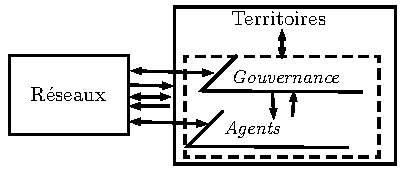
\includegraphics[width=\textwidth]{Figures/Theory/processes_acteurs}
\end{figure}
%%%%%%%%%%%%%


Dans ce schéma, on identifie les acteurs territoriaux au sein du système territorial, qui se déclinent schématiquement sur deux échelles : les agents à l'échelles microscopique qui seront centraux pour les processus de mobilité, et les acteurs de gouvernance à des échelles supérieures, qui mènent les processus de gouvernance. Ils interagissent entre eux de manière complexe, et sont séparés ici conceptuellement par les pointillés d'autre aspects du territoire avec les quels ils sont aussi couplés fortement.


Cette entrée peut être mise en perspective avec le cadre conceptuel de~\cite{le2010approche}, qui étudie les liens entre forme urbaine et pratiques de mobilité dans des contextes métropolitains. Celui-ci comprend le système urbain comme un couplage fort entre système de localisation, système d'activités et système de transport, en précisant l'influence des agents demandeurs (agents micro-économiques) et des agents aménageurs (agents de gouvernance) sur chaque système. Le système de transport correspond à nos réseaux et les deux autres systèmes à un aspect des agents territoriaux, qui contiennent aussi les agents précisés dans ce cadre. Ce parallèle reste à nuancer lorsqu'on change d'échelle : à celle du système de villes, lorsque les agents sont les villes, le système de localisation n'a plus de sens : celui-ci est adapté à une échelle au plus métropolitaine, et surtout aux ontologies correspondantes.


\bigskip

Cette double entrée de lecture des processus d'interaction entre réseaux et territoires conditionnera d'une part la revue de littérature des modèles faite en Chapitre\ref{ch:modelinginteractions}, et sera d'autre part complétée et précisée à l'issue de celui-ci.




%----------------------------------------------------------------------------------------

\newpage


\section*{Chapter Conclusion}{Conclusion du Chapitre}


Les territoires, que nous avons défini comme territoires humains, interagissent de manière complexe avec les réseaux, en particulier ceux de transport, comme montré par les nombreux exemples empiriques ou les constructions théoriques passés en revue. A différentes échelles temporelles typiques, l'année, la décennie et le siècle, correspondent plus ou moins des échelles spatiales : métropolitaine, régionale et système de villes, ainsi que des processus : mobilité, accessibilité et relocalisations, effets systémiques structurels et bifurcations. Les situations concrètes témoignent de réalités locales déclinés avec différentes nuances, et des processus portant ces processus abstraits avec différents rôles et interactions entre eux. Nous avons dans une première section clarifié cette notion d'interaction entre réseaux de transports et territoires en construisant un cadre théorique qui permet de les considérer comme des composantes du système territorial dans son ensemble. Nous avons alors suggéré une approche par la co-évolution pour tenir compte de cette complexité. Afin de mieux cerner ces notions sur des exemples géographiques concrets, nous avons développé en~\ref{sec:casestudies} deux cas d'étude métropolitain d'actualité, et souligné les certitudes en termes d'impact d'accessibilité pour des projets majeurs d'infrastructures qui s'accompagnent systématiquement d'incertitude en terme de trajectoire du système à plus long terme. Enfin, nous proposons en~\ref{sec:qualitative} une excursion par des éléments de terrain dans le Guangdong, Chine. A ce stade, ayant introduit l'objet d'étude thématique, nous proposons de restreindre la portée des entrées prises sur le sujet, et s'intéresser plus particulièrement aux approches impliquant une modélisation, faisant le choix d'un rôle fondamental du \emph{modèle} (sur lequel nous reviendrons plus en détails par la suite) dans la production de connaissance.


% pour limiter les effets d'intermédiaire qui augmenteraient la distance au terrain géographique réel qui est selon~\cite{lefort2012terrain} déjà très présente dans les études le prenant comme matériau empirique principal,




\stars


%-------------------------




%%%%%%%%%%%%%%%%%%%%%%%%%%%%%


%%%%%%%%%%%%%%%%%%%%%%%%%%%%%
% Chapter 2 : Modeling the Interactions


%\chapter{Modeling Interactions between Networks and Territories}{Modéliser les Interactions entre Réseaux et Territoires} % Chapter title
\chapter{Modéliser les Interactions entre Réseaux et Territoires}


\label{ch:modelinginteractions}

%----------------------------------------------------------------------------------------




Si la littérature empirique et thématique, ainsi que les cas d'études développés précédemment\comment[FL]{NB: comme je commence par lire des 2 je ne les ai pas en tete}, semblent converger vers un consensus sur la complexité des relations entre réseaux et territoires\comment[FL]{mots qu'il conviendra d'avoir definis precedemment}, et\comment[FL]{faire deux phrases} dans certaines configurations et à certaines échelles de relations circulaires causales entre dynamiques territoriales et dynamiques des réseaux de transports\comment[FL]{pourquoi dans la premiere partie de la phrase il ny a pas transports et la oui?} que l'on se proposera de désigner par \emph{co-évolution}\comment[FL]{faire une tournure de phrase plus simple pour definir le not coevolution}, ceux-ci semblent diverger sur toute explication potentiellement simple\comment[FL]{mal dit} ou systématique, comme le rappelle par exemple les débats autour des effets structurants des infrastructures~\cite{offner1993effets}\comment[FL]{qu'il convient ici d'expliciter en 2.3 - $\phi$ : qui dit quoi dans ce debat ?}. Au contraire, les multiples situations géographiques poussent à privilégier des études ciblées très fortement dépendantes du contexte et du travail de terrain\comment[FL]{phrase un peu rapide tu donnes l'impression que tu tranches le debat}. Or l'explication géographique et la compréhension des processus est très vite limitée dans cette approche, et intervient un besoin d'un certain niveau d'abstraction et de généralisation\comment[FL]{or justement il convient d'expliciter ce debat theorie vs empirisme (ou autre)$\rightarrow$dans la phrase en pointilles tu parles d'un besoin d'abstraction, ce nest pas le terme scientifique}. C'est sur un tel point que la Théorie Evolutive des Villes se concentre particulièrement\comment[FL]{il faut absolument se departir d'un ton enthousiaste non scientifique. tu te proposes d'appliquer une theorie/un cadre analytique a une question - ca marche plus ou moins, cest tout, il ne doit pas y avoir d'a priori ou de preference de ton cote}, puisqu'elle arrive à combiner des schémas et modèles généraux aux particularités géographiques, et en tire même parti, tandis\comment[FL]{faire deux phrases} que certaines théories issues de la physique comme la Théorie du Scaling de \noun{West}~\cite{west2017scaling} peuvent être plus difficile à digérer pour les géographes\comment[FL]{tu pars deja dans de l'interpretation epistemo : il faut séparer les choses, d'abord de quoi s'agit-il ?} de par leur positionnement d'universalité qui est à l'opposé de leurs épistémologies habituelles. Dans tous les cas, le \emph{medium} qui permet de gagner en généralité sur les processus et structures des systèmes est toujours le \emph{modèle}\comment[FL]{l'italique ne joue pas le meme role pour les 2 mots cela prete a confusion} (voir \ref{sec:knowledgeframework} pour un développement des domaines de connaissance et du rôle du modèle). Comme le rappelle \noun{J.P. Marchand}~\cite{raimbault2017entretiens}, ``notre génération a compris qu'il y avait une co-évolution, la votre cherche à la comprendre''\comment[FL]{TB citation a mettre en italique}, ce qui appuie le pouvoir de compréhension apporté par la modélisation et la simulation qui pourraient être aujourd'hui à leur balbutiements\comment[FL]{ok avec le sens de cette phrase mais le conditionnel sonne mou. si tu as des arguments avance les, sinon dis clairement auelle est ta position}. Sans développer les innombrables fonctions que peut avoir un modèle, nous nous baserons sur l'adage\comment[FL]{terme non scientifique} de \noun{Banos} qui soutient que ``modéliser c'est apprendre'', et suivant notre positionnement dans une science des systèmes complexes suggéré en introduction, nous ferons ainsi de la \emph{modélisation des interactions entre réseaux et territoires} notre principal sujet d'étude, outil, objet (même si dans une lecture rigoureuse de~\ref{sec:knowledgeframework} ce positionnement n'a pas de sens puisque notre démarche contenait déjà des modèles à partir du moment où elle était scientifique\comment[FL]{tu ne peux pas parler d'une lecture rigoureuse de tes propres propos ! supprime la ()}). Ce chapitre peut être vu comme un ``état de l'art'' des démarches de modélisation des interactions entre réseaux et territoires. Il vise en particulier à être aussi objectif et exhaustif que possible\comment[FL]{mal amene, cest souvent le but non ?} : pour cela, nous mobiliserons des analyses en épistémologie quantitative. Dans une première section~\ref{sec:modelingsa}, nous passons en revue de manière interdisciplinaire les modèles pouvant être concernés, même de loin, sans a priori d'échelle temporelle ou spatiale, d'ontologies, de structure, ou de contexte d'application. Les modèles de changement d'usage du sol très appliqués en planification sont tout autant concernés que des modèles totalement abstraits issus de la biologie ou de la physique, que des approches intégrées en géographie ou spécifiques en économie\comment[FL]{pas utile ici tu detailleras en 2.1 : ici affirmer les objectifs (quelle information en retirer) et les moyens (par ez meme automatique tu as bien un (des) points d'entrees $\rightarrow$ lesquels et pourquoi?}. Cet aperçu suggère des structures de connaissances assez indépendantes et des disciplines ne communiquant que rarement\comment[FL]{B}. Nous procédons à une revue systématique algorithmique\comment[FL]{est-ce une facon standard de nommer cela ?}[(JR) l'exploration iterative de la facon dont elle est faite n'a jamais ete faite a ma connaissance, j'introduis donc une ``nouvelle'' façon de faire.] dans~\ref{sec:quantepistemo} pour reconstruire leur paysage scientifique, dont les résultats tendent à confirmer ce cloisonnement\comment[FL]{c'est interessant bien sur mais il faut dire pourquoi tu vises cela. a mon avis il vaut mieux commencer par des exemples de manieres dont la litterature sci. prend en compte ces interactions, dans differentes disciplines, avant d'atteindre l'epistemologie quantitative.}. L'étude est complétée par une analyse d'hyperréseau, combinant réseau de citation et réseau sémantique issu d'analyse textuelle, qui permet de mieux cerner les relations entre disciplines, leur champs lexicaux et leur motifs d'interdisciplinarité. Cette étude permet la constitution du corpus utilisé pour la modélographie et la meta-analayse\comment[FL]{mots qui nont pas encore ete introduits} effectuée en dernière section~\ref{sec:modelography}, qui dissèque la nature d'un certain nombre de modèles et la relie au contexte disciplinaire, ce qui pose les bases et le cadre précis des efforts de modélisation qui seront développés par la suite.






\stars


\textit{Ce chapitre est inédit pour sa première section ; reprend dans sa deuxième section le texte traduit de~\cite{raimbault2015models}, puis pour sa deuxième partie la méthodologie de \cite{raimbault2016indirect}, les outils de \cite{bergeaud2017classifying} et des passages de~\cite{}; et est enfin inédit pour sa dernière partie.}

\comment[FL]{mettre bout a bout tous ces passages (non classiques, mais que je trouve beinvenus, en toute fin d'intro generale)}[à rediscuter, je trouve ca plus adapté pour chaque chapitre dans le cadre d'une ``these a papiers'' (meme si c'est est pas une officiellement).]







%
% 2.1 - State of the Art




%----------------------------------------------------------------------------------------

\newpage

\section{Modeling Interactions}{Modéliser les Interactions}
\label{sec:modelingsa}


%----------------------------------------------------------------------------------------




\subsection{Modeling in Quantitative Geography}{Modélisation en Géographie Quantitative}


\subsubsection{History}{Histoire}

\bpar{
Modeling in Theoretical and Quantitative Geography (TQG), and more generally in Social Science, has a long history on which we can not go further than a general context. \noun{Cuyala} does in~\cite{cuyala2014analyse} an analysis of the spatio-temporal development of French speaking TQG movement and underlines the emergence of the discipline as the combination between quantitative analysis (e.g. spatial analysis or modeling and simulation practices) and theoretical constructions, an integration of both allowing the construction of theories from empirical stylized facts that yield theoretical hypothesis to be tested on empirical data. These approach were born under the influence of the \emph{new geography} in Anglo-saxon countries and Sweden.
}{
La modélisation joue en Géographie Théorique et Quantitative (TQG) un rôle fondamental. \cite{cuyala2014analyse} procède à une analyse spatio-temporelle du mouvement de la Géographie Théorique et Quantitative en langue française et souligne l'émergence de la discipline comme une combinaison d'analyses quantitatives (e.g. analyse spatiale et pratiques de modélisation et de simulation) et de construction théoriques. Cette dynamique est datée à la fin des années 70, et est intimement liée à l'utilisation et l'appropriation des outils mathématiques~\cite{pumain2002role}. L'intégration de ces deux composantes permet la construction de théories à partir de faits stylisés empiriques, qui produisent à leur tour des hypothèses théoriques pouvant être testées sur les données empiriques. Cette approche est née sous l'influence de la \emph{New Geography} dans les pays Anglo-saxons et en Suède. Concernant la modélisation urbaine en elle-même, d'autre champs que la géographie ont proposé des modèles de simulation à peu près à la même période. Par exemple, le modèle de \noun{Lowry}, développé par~\cite{lowry1964model} dans un but appliqué immédiat à la région métropolitaine de Pittsburg, suppose un système d'équations pour la localisation des actifs et des emplois dans différente zones. Des modèles relativement similaires sont toujours utilisés aujourd'hui.\comment[FL]{modele de Lowry c'est abscons}
}




%\comment[FL]{manque peut etre quelques phrases avec des modeles ``landmark'' anciens (Lowry 1964 par exemple) mais encore utilises, de plus ne pas perdre le fil du champ applicatif auquel tu te destines}

% Lowry : https://www.rand.org/content/dam/rand/pubs/research_memoranda/2006/RM4035.pdf
% Alonso : http://onlinelibrary.wiley.com/doi/10.1111/j.1435-5597.1967.tb01370.x/epdf
% http://www.sciencedirect.com/science/article/pii/S009411909792074X prefatt-diff ?


\subsubsection{Simulation of models and intensive computation}{Simulation de modèle et calcul intensif}


\bpar{
A broad history of the genesis of models of simulation in geography is done by \noun{Rey} in~\cite{rey2015plateforme} with a particular emphasis on the notion of validation of models. The use of computation for simulation of models is anterior to the introduction of paradigms of complexity, coming back to \noun{H{\"a}gerstrand} and \noun{Forrester}, pioneers of spatial economic models inspired by Cybernetics. With the increase of computational possibilities epistemological transformations have also occurred, with the apparition of explicative models as experimental tools. \noun{Rey} compares the dynamism of seventies when computation centers were opened to geographers to the democratization of High Performance Computing (transparent grid computing, see~\cite{schmitt2014half} for an exemple of the possibilities offered in terms of model validation and calibration, decreasing the computational time from 30 years to one week), that is also accompanied by an evolution of modeling practices~\cite{banos2013pour} and techniques~\cite{10.1371/journal.pone.0138212}.
}{
Une histoire étendue de la genèse des modèles de simulation en géographie est faite par \noun{Rey} dans~\cite{rey2015plateforme} avec une attention particulière pour la notion de validation de modèles (nous reviendrons sur la place de ces aspects dans notre travail en~\ref{ch:positioning}). L'utilisation de ressources de calcul pour la simulation de modèles est antérieure à l'introduction des paradigmes de la complexité actuels, remontant par exemple à \noun{Forrester}, informaticien qui a été pionnier des modèles d'économie spatiale inspirés par la cybernétique\footnote{Celle-ci, ainsi que le courant systémique, sont comme nous l'avons déjà développé précurseurs des paradigmes actuels de la complexité.}. Avec l'augmentation des potentialités de calcul, des transformations épistémologiques ont également suivi, avec l'apparition de models explicatifs comme outils expérimentaux. \noun{Rey} compare le dynamisme des années soixante-dix quand les centres de calcul furent ouverts aux géographes à la démocratisation actuelle du Calcul Haute Performance\footnote{Le développement des premiers modèles de simulation urbaine coincide avec l'ouverture des premiers centres de calcul aux sciences humaines, comme le rappelle par ailleurs \noun{Pumain} (entretien du ) par exemple pour l'implémentation du modèle d'entropie d'\noun{Allen}.}\comment[FL]{il faut que tu detailles}. Aujourd'hui, cette facilité d'accès consiste entre autres à du calcul sur grille dont l'utilisation est rendue transparente, c'est à dire sans besoin de compétences techniques pointues liées au mécanismes de la distribution des calculs.. Ainsi~\cite{schmitt2014half} donnent un exemple des possibilités offertes en termes de calibration et de validation de modèle, réduisant le temps de calcul nécessaire de 30 ans à une semaine - ces techniques jouent un rôle clé pour les résultats que nous obtiendrons par la suite. Cette évolution est également accompagnée par une évolution des pratiques~\cite{banos2013pour} et techniques~\cite{10.1371/journal.pone.0138212} de modélisation.
}


\bpar{
Modeling (in particular computational models of simulation) is seen by many as a fundamental building brick of knowledge : \cite{livet2010} recalls the combination of empirical, conceptual (theoretical) and modeling domains with constructive feedbacks between each. A model can be an exploration tool to test assumptions, an empirical tool to validate a theory against datasets, an explicative tool to reveal causalities (and thus internal processes of a system), a constructive tool to iteratively build a theory with an iterative construction of an associated model. These are example among others : \noun{Varenne} proposes in~\cite{varenne2010simulations} a refined classifications of diverse functions of a model. We will consider modeling as a fundamental instrument of knowledge on processes within complex adaptive systems, as already evoked, and restraining again our question, will focus on \emph{models involving interactions between transportation networks and territories}.
}{
La modélisation, et en particulier les modèles de simulation, est vue par beaucoup comme une brique fondamentale de la connaissance : \cite{livet2010} rappelle la combinaison des domaines empirique, conceptuel (théorique) et de la modélisation, avec des retroactions constructives entre chaque. Un modèle peut être un outil d'exploration pour tester des hypothèses, un outil empirique pour valider une théorie sur des jeux de données, un outil explicatif pour révéler des causalités et ainsi des processus internes au système, un outil constructif pour construire itérativement une théorie conjointement avec celle des modèles associés. Ce sont des exemples de fonctions parmi d'autres : \cite{varenne2010simulations} propose une classification des diverses fonctions d'un modèle. Nous considérons la modélisation comme un instrument fondamental de connaissance des processus au sein d'un système, plus particulièrement dans notre cas au sein d'un système complexe adaptatif. Nous rappelons ainsi que notre question de recherche s'intéressera aux \emph{modèles dont l'ontologie contient une part non négligeable d'interactions réseaux et territoires}.
}




%%%%%%%%%%%%%%%%%%%%%%%%%%%
\subsection{Modeling Territories and Networks}{Modéliser les territoires et réseaux}


\bpar{
Concerning our precise question of interactions between transportation networks and territories, we propose an overview of existing approaches. Following~\cite{bretagnolle2002time}, the ``\textit{thoughts of specialists in planning aimed to give definitions of city systems, since 1830, are closely linked to the historical transformations of communication networks}''. It is not far from an reversed self-realizing prophecy, in the sense that it is already realized before happening. It implies that ontologies and corresponding models addressed by geographers and planners are closely linked to their current historical preoccupations, thus necessarily limited in scope and purpose. In a perspectivist vision of science~\cite{giere2010scientific} such boundaries are the essence of the scientific entreprise, and as we will argue in chapter~\ref{ch:theory} their combination and coupling in the case of models is a source of knowledge.
}{
Développons à présent un aperçu des différentes approches modélisant des interactions entre réseaux de transport et territoires. Remarquons de manière préliminaire une forte contingence des constructions scientifiques sous-jacentes à celles-ci. En effet, selon~\cite{bretagnolle2002time}, ``\textit{les idées des spécialistes de la planification cherchant à donner des définitions des systèmes de ville, depuis 1830, sont étroitement liées aux transformations des réseaux de communication}''. Le contexte historique (et donc socio-économique et technologique) conditionne fortement les théories formulées. Cela implique que les ontologies et les modèles correspondants proposés par les géographes et les planificateurs sont fortement liés aux préoccupations historiques courantes, ce qui limite nécessairement leur portée théorique et/ou opérationnelle. Au delà de la question de la définition du système qui joue également un rôle central, on comprend bien l'impact que peut avoir cette influence sur la portée des modèles développés. Dans une vision perspectiviste de la science~\cite{giere2010scientific} de telles limites sont l'essence de l'entreprise scientifique, et comme nous démontrerons dans le chapitre~\ref{ch:theory} leur combinaison et couplage dans le cas de modèles est généralement une source de connaissance.
}


%C'est en quelque sorte la prophétie auto-réalisatrice inversée, au sens où elle est déjà réalisée avant d'être formulée\comment[FL]{sens ?}. % -> notion de coevol des connaissance avec les objets - on revient sur la reflexivité - trop glissant pour développer.

% \comment[FL]{pas par essence mais cela peut l'etre effectivement}[(JR) pas d'accord : opérer un couplage de modele implique un couplage des ontologies et necessairement un accroissement des connaissances (si celui-ci est utile c'est un autre problème)]


L'entrée que nous proposons ici pour dresser un aperçu des modèles est complémentaire de celle prise au Chapitre~\ref{ch:thematic}, en regardant par objet principal (c'est à dire les relations Réseau $\rightarrow$ Territoire, Territoire $\rightarrow$ Réseau et Territoire $\leftrightarrow$ Réseau)\footnote{Nous rappelons la signification de cette notation introduite au Chapitre~\ref{ch:thematic} : une flèche directe signifie des processus qu'on peut attribuer relativement de manière univoque à l'origine, tandis qu'une flèche réciproque suppose intrinsèquement l'existence d'interactions réciproques, généralement en coincidence avec l'émergence d'entités jouant un rôle dans celles-ci.}. Nous avons vu que la correspondance à des échelles temporelles et spatiales n'est pas systématique (voir la typologie provisoire à double entrée des processus). Par contre, celle à des domaines particuliers et à des acteurs l'est plus. Cette revue de littérature est donc orientée dans cette seconde direction.

%\comment[FL]{tu arrives trop tot la dessus - les processus cles ne sont pas ammenes suffisamment clairement : travaille par echelle de temps, d'espace, d'acteurs}[ok developper en echo au 1 - vision par les acteurs / vision par les echelles.]


%\subsubsection{Land-Use Transportation Interaction Models}{Modèles LUTI}
\subsubsection{Territories}{Territoires}


Le courant principal s'intéressant à la modélisation de l'influence du réseau de transport sur les territoires se trouve dans le champ de la planification, à des échelles spatiales et temporelles moyennes (les échelles de l'accessibilité métropolitaine que nous avons développés ci-dessus). Des modèles en géographie à d'autres échelles, comme les modèles Simpop déjà évoqués~\cite{pumain2012multi}, ne supposent pas une ontologie particulière pour le réseau de transport, et s'ils incluent des réseaux entre les villes comme porteur des échanges, ne permettent cependant pas d'étudier en particulier les relations entre réseaux et territoires. Nous reviendrons plus loin sur des extensions pertinentes pour notre question. Revoyons pour commencer un contexte de modèles plus proches des études de planification.


\paragraph{LUTI models}{Modèles LUTI}

\bpar{
A subsequent bunch of literature in modeling interaction between networks and territories can be found in the field of planning, with the so-called \emph{Land-use Transportation Interaction Models}. These works are difficult to be precisely bounded as they may be influenced by various disciplines. For example, from the point of view of Urban Economics, propositions for integrated models have existed for a relatively long term~\cite{putman1975urban}.
}{
Ces approches sont désignées de manière générale comme \emph{modèles d'interaction entre usage du sol et transport} (\emph{LUTI}, pour \textit{Land-Use Transport Interaction}). Il est entendu par usage du sol la répartition des activités territoriales, généralement réparties en typologies plus ou moins précises (par exemple logements, industrie, tertiaire, espace naturel). Ces travaux peuvent être difficiles à cerner car liés à différentes disciplines scientifiques. Leur principe général est de modéliser et simuler l'évolution de la distribution spatiale des activités, en prenant le réseau de transport comme contexte et déterminant significatif des localisations. Par exemple, du point de vue de l'Economie Urbaine, les propositions de tels modèles existent depuis un certain temps : \cite{putman1975urban} rappelle le cadre d'économie urbaine où les principales composantes sont les emplois, la démographie et le transport, et passe en revue des modèles économiques de localisation qui s'apparentent au modèle de \noun{Lowry}.
}


\bpar{
Generally these type of models operate at relatively small temporal and spatial scales. \cite{wegener2004land} reviewed state of the art in empirical and modeling studies on interactions between land-use and transportation. It is positioned in economic, planning and sociological theoretical contexts, and is relatively far from our geographical approach aiming to also understand long-time processes. Seventeen models are compared and classified, none of which implements actually network endogenous evolution on the relatively small time scales of simulation. A complementary review done in \cite{chang2006models} broadens the scope with inclusion of more general classes of models, such as spatial interaction models (including traffic assignment and four steps models), operational research planning models (optimal localisations), micro-based random utility models, and urban market models.
}{
\cite{wegener2004land} donne plus récemment un état de l'art des études empiriques et de modélisation sur ce type d'approche des interactions entre usage du sol et transport.\comment[FL]{Wegener et furst traite bcp trop succintement. il faut expliciter ce qu'il y a dedans pas attendre de ton lecteur qu'il l'ai lu} Le positionnement théorique est plutôt proche des disciplines de la socio-économie des transports et de la planification (voir les paysages disciplinaires dressés en~\ref{sec:quantepistemo}). \cite{wegener2004land} compare et classifie dix-sept modèles, parmi lesquels aucun n'inclut une évolution endogène du réseau de transport sur les échelles de temps relativement courtes (de l'ordre de la décade) des simulations. On retrouve bien la correspondance avec les échelles typiquement mesoscopiques établies précédemment. Une revue complémentaire est faite par~\cite{chang2006models}, élargissant le contexte avec l'inclusion de classes plus générales de modèles, comme des modèles d'interactions spatiales (parmi lesquels l'attribution du traffic et les modèles à quatre temps), les modèles de planification basés sur la recherche opérationnelle (optimisation des localisations des différentes activités, généralement résidences et emplois), les modèles microscopiques d'utilité aléatoire, et les modèles de marché foncier.
}

\comment[FL]{dire que luti c'est largement etudie me semble très exagéré il n'y a pas vraiment beaucoup de modèles existants dans le monde}


\comment[JR]{comment peut-on dire / pourquoi dit-on que luti est une classe ? necessiterait une etude ciblée...}

Afin de donner une meilleure intuition de la logique sous-jacente à un modèle Luti, nous détaillons en Encadré~\ref{frame:modelingsa:luti} la structure et les hypothèses de deux modèles développés dans le cas spécifique de l'Ile-de-France.




%%%%%%%%%%%%%%
\begin{figure}[h!]
	\begin{mdframed}
	
	\cite{delons:hal-00319087} pirandello
	
	\cite{viguie2014downscaling} Nedum
	
	% couplage avec modus http://www.agence-nationale-recherche.fr/Projet-ANR-14-CE22-0013
	% seminaire lvmt (27/11) : points cruciaux soulevés
	%  - endogeneite de la gouvernance, ou le sdrif sert-il a rien ? accompagne dynamique locale. negociations locales. modele calibre sur amenagements passes : le sdrif n'est pas une rupture : dynamique sur le temps long intrinseque, capturee par le modele.
	%  - difficulte technique du couplage : ouverture etc
	%  - question endogeneite : White, exploration modeles, mutlimodeling, parcimonie.
	%  - difficulte ontologique du couplage : modele ont processus oppose, instable numeriquement : domaines de validités locaux ? (au sens des hypotheses) - en ouverture : enrome a travail a faire sur le couplage, du point de vue des domaines de connaissance (differentes dimensions du couplage)
	
	\medskip
	
	\framecaption{}{\textbf{Les Luti pour l'Ile-de-France : de Pirandello à Nedum.}\label{frame:modelingsa:luti}}
	
	\end{mdframed}
\end{figure}
%%%%%%%%%%%%%%



\paragraph{Operational models}{Des modèles opérationnels très variés}


\bpar{The variety of possible models has lead to operational comparisons~\cite{paulley1991overview,wegener1991one}.}
{
La variété des modèles existants a conduit à des comparaisons opérationnelles : \cite{paulley1991overview} rendent compte d'un projet comparant différents modèles appliqués à différentes villes. Leurs résultats permettent d'un part de classifier des interventions en fonction de leur impact sur le niveau d'interaction entre transport et usage du sol, et d'autre part de montrer que l'effet des interventions dépend fortement de la taille de la ville et de ses caractéristiques socio-économiques.
}


\bpar{
More recently, the respective advantages of static and dynamic modeling was investigated in~\cite{kryvobokov2013comparison}.
}{
Les ontologies des processus, et notamment sur la question de l'équilibre, sont aussi variées. Les avantages respectifs d'une approche statique (calcul d'un équilibre statique de la localisation des ménages pour une certaine spécification de leur fonctions d'utilité) et d'une approche dynamique (simulation hors équilibre des dynamiques résidentielles) a été étudié par~\cite{kryvobokov2013comparison}, dans un cadre métropolitain sur des échelles de temps de l'ordre de la décade. Les auteurs montrent que les résultats sont globalement comparables et que chaque modèle a son utilité selon la question posée.
}



\bpar{
These techniques operate also at small scales and consider at most land-use evolution. \cite{iacono2008models} covers a similar scope with a further emphasis on cellular automata models of land-use change and agent-based models. These type of models are still largely developed and used today, as for example \cite{delons:hal-00319087} which is used for Parisian metropolitan region. The short-term range of application and their operational character makes them useful for planning, what is far from our preoccupation to obtain explicative models for geographical processes.
}{
Différents aspects du même système peuvent être traduits par divers modèles, comme le montre par exemple~\cite{wegener1991one}, et le trafic, les dynamiques résidentielles et d'emploi, l'évolution de l'usage du sol en découlant, influencée aussi par un réseau de transport statique, sont généralement pris en compte. \cite{iacono2008models} couvre un horizon similaire avec un développement supplémentaire sur les modèles à automates cellulaires d'évolution d'usage du sol et les modèles à base d'agents. Les modèles LUTI sont toujours largement étudiés et appliqués, comme par exemple \cite{delons:hal-00319087} qui est utilisé pour la région métropolitaine parisienne. La portée temporelle d'application de ces modèles, de l'ordre de la décade, et leur nature opérationnelle les rend utiles pour la planification, ce qui est assez loin de notre souci d'obtenir des modèles explicatifs de processus géographiques. En effet, il est souvent plus pertinent pour un modèle utilisé en planification d'être lisible comme outil d'anticipation, voire de communication, que d'être fidèle aux processus territoriaux au prix d'une abstraction.
}



\paragraph{Perspectives for LUTI models}{Perspectives pour les LUTI}

\bpar{}{
\cite{timmermans2003saga} émet des doutes quant à la possibilité de modèles d'interaction réellement intégrés, c'est à dire produisant des motifs de transports endogènes et se détachant d'artefacts comme l'accessibilité dont l'influence du caractère artificiel reste à établir, notamment à cause du manque de données et une difficulté à modéliser les processus de gouvernance et de planification. Il est intéressant de noter que les priorités actuelles de développement des modèles LUTI semblent centrées sur une meilleure intégration des nouvelles technologies et une meilleur intégration avec la planification et les processus de prise de décision, par exemple via des interfaces de visualisation comme le propose~\cite{JTLU611}. Ils ne cherchent pas à s'étendre à des problématiques de dynamiques territoriales incluant le réseau sur de plus longues échelles par exemple, ce qui confirme la portée et la logique d'utilisation et de développement de ce type de modèles.
}

\bpar{}{
Une généralisation de ce type d'approche à une plus grande échelle, comme celle proposée par \cite{russo2012unifying}, consiste au couplage du LUTI à l'échelle mesoscopique à des modèles macroéconomiques à l'échelle macroscopique.\comment[FL]{modele de russo et musolino a detailler ce n'est pas comprehensible} Ceux-ci ne considèrent pas l'évolution du réseau de transport de manière explicite mais s'intéressent seulement aux motifs abstraits d'offre et demande. L'économie urbaine a développé des approches spécifiques similaires dans leur démarche : \cite{masso2000} décrit par exemple un modèle intégré couplant développement urbain, relocalisation et équilibre des flux de transports.
}


\bpar{}{
Ainsi, nous pouvons synthétiser ce type d'approche, qu'on pourra désigner par abus de langage \emph{approche LUTI}, par les caractéristiques fondamentales suivantes : (i) Modèles visant à comprendre une évolution du territoire, dans le contexte d'un réseau de transport donné ; (ii) Modèles dans une logique de planification et d'applicabilité, étant souvent impliqués eux-même dans les prises de décision ; et (iii) Modèles à des échelles moyennes, dans l'espace (métropole) et dans le temps (décade).
}

\comment[FL]{tu parles et c'est tres bien d'echelle d'espace et de temps moyenne. Cela doit etre amene ; quelle matrice adoptes tu pour parler de ces echelles? cela doit etre explicite avant}[lecture ch1 - a expliciter ou rappeler ?]



\subsubsection{Network Growth}{Croissance du Réseau}

Passons à présent au paradigme ``opposé'', centré sur l'évolution du réseau. Il peut sembler incongru de considérer un réseau variable en négligeant les variations du territoire, au regard de l'aperçu de certains des mécanismes potentiels d'évolution revus précédemment (rupture de potentiel, auto-renforcements, planification du réseau) qui se produisent à des échelles de temps majoritairement plus longues que les évolutions territoriales. On verra ici qu'il n'y a pas de paradoxe, vu que (i) soit la modélisation s'intéresse à l'évolution des \emph{propriétés du réseau}, à une courte échelle (micro) pour des processus de congestion, de capacité, de tarification, principalement d'un point de vue économique ; (ii) soit les composantes territoriales jouant en effet sur le réseau sont stables au échelles longues considérés (approches des physiciens\comment[FL]{dire approche des physiciens est reductuer}).


\bpar{
Network growth can be used to design modeling entreprises that aim to endogenously explain growth of transportation networks, generally from a bottom-up point of view, i.e. by exhibiting local rules that would allow to reproduce network growth over long time scales (generally the road network).
}{
La croissance de réseaux est l'objet de démarches de modélisation qui cherchent à expliquer la croissance des réseaux de transport. Ils prennent généralement un point de vue \emph{bottom-up} et endogène, c'est-à-dire cherchant à mettre en évidence des règles locales qui permettraient de reproduire la croissance du réseau sur de longues échelles de temps (souvent le réseau routier). Comme nous allons le voir, il peut s'agir de la croissance topologique (création de nouveaux liens) ou la croissance des capacités des liens en relation avec leur utilisation, selon les échelles et les ontologies considérées. Nous distinguons pour simplifier des grands courants disciplinaires s'étant intéressé à la modélisation de la croissance des réseaux de transport : ceux-ci sont liés respectivement à l'économie des transports, la physique, la géographie des transport et la biologie.
}


\bpar{
\cite{xie2009modeling} develops a broad review on network growth modeling extending to other fields: transportation geography early developed empirical-based models but which did concentrate on topology reproduction rather than on mechanisms according to~\cite{xie2009modeling}; statistical models on case studies provide mitigated conclusions on causal relations between offer and demand; economists have studied infrastructure provision from both microscopic and macroscopic point of views, generally non-spatial; network science has provided toy-models of network growth based on structural and topological rules rather on rules inspired from real processes.
}{
On rejoint ainsi partiellement la classification de~\cite{xie2009modeling}, qui propose une revue étendue de la modélisation de croissance des réseaux, dans une perspective d'économie des transports mais en élargissant à d'autres champs. Selon~\cite{xie2009modeling}, la géographie des transports a développé très tôt des modèles basés sur des faits empiriques mais qui ont visé à reproduire la topologie plutôt que sur les mécanismes ; les modèles statistiques sur des cas d'étude fournissent des conclusions très mitigées sur les relations causales entre croissance du réseau et demande (la croissance étant dans ce cas conditionnée aux données de demande) ; les économistes ont étudié la production d'infrastructure à la fois d'un point de vue microscopique et macroscopique, généralement non spatialisés ; la science des réseaux a produit des modèles stylisés de croissance de réseau qui se basent sur des règles topologiques et structurelles plutôt que des règles se reposant sur des processus correspondant à des réalités empiriques.
}

\comment[FL]{cette partie avant economie : tres utile overview. il manque au tout debut, il me semble pas logique que ca vienne apres les luti en detail}


\paragraph{Economics}{Economie}

\bpar{
Economists have proposed such models: \cite{zhang2007economics} reviews transportation economics literature on network growth within an endogenous growth theory~\cite{aghion1998endogenous}, recalling the three main features studied by economists on that subject that are road pricing, infrastructure investment and ownership regime, and describes an analytical model combining the three. An other approach not mentioned that we will develop further is biologically inspired network design. We first give some example of economic-based and geometrical-based network growth modeling attempts. \cite{yerra2005emergence} shows through a reinforcement economic model including investment rule based on traffic assignment that local rules are enough to make hierarchy of roads emerge for a fixed land-use.
}{
Les économistes ont proposé des modèles de ce type : \cite{zhang2007economics} passe en revue la littérature en Economie des Transports sur la croissance des réseaux, rappelant les trois aspects principalement traités par les économistes sur le sujet, qui sont la tarification routière, l'investissement en infrastructures et le régime de propriété, et propose finalement un modèle analytique combinant les trois. Ces trois classes de processus relèvent d'une interaction entre les agents économiques microscopiques (utilisateurs du réseau) et les agents de gouvernance. Les modèles peuvent inclure une description détaillée des processus de planification, comme~\cite{levinson2012forecasting} qui combine des enquêtes qualitatives et des statistiques pour paramétrer un modèle de croissance de réseau. \cite{xie2009jurisdictional} compare l'influence relative des processus de croissance centralisés (planification par une structure de gouvernance) et décentralisés (croissance locale ne rentrant pas dans le cadre d'une planification globale). \cite{levinson2003induced} procède à une étude empirique des déterminants de la croissance du réseau routier pour les \emph{Twin Cities} aux Etats-Unis (Minneapolis-Saint-Paul), établissant que les variables basiques (longueur, changement dans l'accessibilité) ont le comportement attendu, et qu'il existe une différence entre les niveaux d'investissement, impliquant que la croissance locale n'est pas affectée par les coûts, ce qui peut correspondre à une équité des territoires en termes d'accessibilité. Ces données sont utilisées par~\cite{zhang2016model} pour calibrer un modèle de croissance de réseau qui superpose les décisions d'investissement aux motifs d'utilisation du réseau. \cite{yerra2005emergence} montre avec un modèle économique basé sur des processus d'auto-renforcement (c'est à dire incluant une rétroaction positive des flux sur la capacité) et incluant une règle d'investissement basée sur l'attribution du trafic, que des règles locales sont suffisantes pour faire émerger une hiérarchie du réseau routier à usage du sol fixé. Une synthèse de ces travaux gravitant autour de \noun{Levinson} est faite dans~\cite{xie2011evolving}.
}

% sur ownership structure et pricing :
% https://sci-hub.cc/https://link.springer.com/article/10.1007/s11067-015-9309-3
% relié à gouvernance, mais trop loin du sujet ici.


\paragraph{Physics}{Physique}

\bpar{
A very similar model in~\cite{louf2013emergence} with simpler cost-benefits obtains the same conclusion.
}{
La physique a introduit récemment des modèles de croissance des réseaux d'infrastructure, em s'inspirant largement de cette littérature économique : un modèle très similaire au dernier cité est donné par~\cite{louf2013emergence} avec des fonctions coûts-bénéfices plus simples mais obtenant une conclusion similaire. Etant donné une distribution de noeuds (villes)\footnote{On se trouve ici dans un cas où l'hypothèse de non-évolution des population des villes tandis que le réseau s'établit itérativement trouve peu de support empirique ou thématique, puisqu'on a montré que réseau et villes avaient des échelles de temps d'évolution comparables. Ce modèle produit donc plus à proprement parler un \emph{réseau potentiel} étant donné une distribution de villes, et il est à interpréter avec précaution.} dont la population suit une loi puissance, deux villes seront connectées par un lien routier si une fonction d'utilité coût-bénéfice, combinant linéairement flux gravitaire potentiel et coût de construction\footnote{Ce qui donne une fonction de coût de la forme $C = \beta / d_{ij}^{\alpha} - d_{ij}$, où $\alpha$ et $\beta$ sont des paramètres}, a une valeur positive. Ces hypothèses locales simples suffisent à faire émerger un réseau complexe et des transitions de phase en fonction du paramètre de poids relatif dans le coût, conduisant à l'apparition de la hiérarchie. \cite{zhao2016population} applique ce modèle de manière itérative pour connecter des zones intra-urbaines, et montre que la prise en compte des populations dans la fonction de coût change significativement les topologies obtenues.
}



\bpar{
Whereas these models based on processes focus on reproducing macroscopic patterns of networks (typically scaling), geometrical optimization models aim to ressemble topologically real networks. \cite{barthelemy2008modeling} proposes a model based on local energy optimization but it stays very abstract and unvalidated. The morphogenesis model given in~\cite{courtat2011mathematics} using local potential and connectivity rules, even if not calibrated, seems to reproduce more reasonably real street patterns. Very close work is done in~\cite{rui2013exploring}.
}{
Une autre classe de modèles, proche dans leur idée des modèles procéduraux, se basent sur des processus d'optimisation géométrique locale, et visent à ressembler à des réseaux réels dans leur topologie. \cite{2016arXiv160906470B} étudie ainsi un modèle de croissance d'arbre appliqué aux pistes de fourmis, dans lequel coût de maintenance et coût de construction influencent tous les deux les choix de nouveau lien. \cite{barthelemy2008modeling} décrit un modèle basé sur une optimisation locale de l'énergie qui génère des réseaux routiers à l'aspect globalement crédible. Le modèle de morphogenèse de~\cite{courtat2011mathematics} qui utilise des potentiels locaux\comment[FL]{pas clair ce que cela signifie} et des règles de connectivité, même s'il n'est pas calibré, reproduit de manière stylisée des motifs réels des réseaux de rues. Un modèle très proche est décrit dans~\cite{rui2013exploring}, tout en incluant des règles supplémentaires pour l'optimisation locale (prise en compte du degré pour la connection de nouveaux liens). La conception optimale de réseau, plutôt pratiquée par l'ingénierie, utilise des paradigmes similaires : \cite{vitins2010patterns} explore l'influence de différentes règles d'une grammaire de formes (notamment les motifs de connection entre les liens de différents niveaux hiérarchiques) sur les performances de réseaux générés par algorithme génétique.
}

\comment[FL]{il faut detailler certains modeles dans un but de clarte du propos. a bien choisir}

% engineering : congestion / capacity
% http://www.sciencedirect.com/science/article/pii/S1877705816003131

%  La simplicité des hypothèses dans ce genre de modèle permet dans certains cas d'inclure des processus qui serait par ailleurs difficile à intégrer : 






%\paragraph{Transport geography}{Géographie des transports}

% la géographie des transports a développé très tôt des modèles basés sur des faits empiriques mais qui ont visé à reproduire la topologie plutôt que sur les mécanismes
% \comment[FL]{point tres important faire une section a part}

% Un peu de geo dans Ducruet :
% https://halshs.archives-ouvertes.fr/file/index/docid/605653/filename/Ducruet_Lugo_SAGE_Handbook_of_Transport_Studies_draft.pdf
% mais sinon remonte majoritairement a Hagget et Chorley, et des travaux contemporains lies a modelisation procedurale






\paragraph{Biological networks}{Réseaux biologiques}


\bpar{
Finally, an interesting and original approach to network growth are biological networks. These belong to the field of morphogenetic engineering pioneered by \noun{Doursat} that aim to design artificial complex system inspired from natural complex systems and in which a control of emerging properties is possible~\cite{doursat2012morphogenetic}. \emph{Physarum Machines}, that are models of a self-organized mould (slime mould) have been shown to provide efficient bottom-up solution to computationally heavy problems such as routing problems~\cite{tero2006physarum} or NP-complete navigation problems such as the Travelling Salesman Problem~\cite{zhu2013amoeba}. It has been shown to produce networks with Pareto-efficient cost-robustness properties~\cite{tero2010rules}, relatively close in shape to real networks (under certain conditions, see~\cite{adamatzky2010road}). This type of models can be of interest for us since auto-reinforcement mechanisms based on flows are analog to mechanisms of link reinforcement in transportation economics.
}{
Enfin, une approche originale et intéressante pour la croissance des réseaux est le réseau biologique. Cette approche appartient au champ de l'ingénierie morphogénétique, qui vise à concevoir des systèmes complexes artificiels inspirés de systèmes complexes naturels et sur lesquels un contrôle des propriétés émergentes est possible~\cite{doursat2012morphogenetic}. Les \emph{Machines Physarum}, qui sont des modèles d'une moisissure auto-organisée (\emph{slime mould}) ont été prouvés comme résolvant de manière efficiente des problèmes difficiles (au sens de leur complexité computationnelle, voir~\ref{sec:epistemology}) comme des problème de routage~\cite{tero2006physarum} ou des problèmes de navigation NP-complets comme le Problème du Voyageur de Commerce~\cite{zhu2013amoeba}. Ces propriétés permettent à ces systèmes de produire des réseaux ayant des propriétés de coût-robustesse Pareto-efficientes~\cite{tero2010rules} qui sont typiques des propriétés empiriques des réseaux réels, et de plus relativement proches en forme de ceux-ci (sous certaines conditions, voir~\cite{adamatzky2010road}).
}

\bpar{}{
Ce type de modèles peut être d'intérêt dans notre cas puisque les processus d'auto-renforcement basés sur les flots sont analogues aux mécanismes de renforcement de lien en économie des transports. Ce type d'heuristique a été testé pour générer le réseau ferré Français par~\cite{mimeur:tel-01451164}, faisant un pont intéressant avec les modèles d'investissement de \noun{Levinson} décrits précédemment\footnote{Sachant que pour cette étude, les critères de validation appliqués restent toutefois limités, soit à un niveau inadapté aux faits stylisés étudiés (nombre d'intersection ou de branches) soit trop générales pouvant être produit par n'importe quel modèle (longueur totale et pourcentage de population desservie), et relèvent de critère de forme typique de la modélisation procédurale qui ne peuvent que difficilement rendre compte des dynamiques internes d'un système comme développé précédemment. De plus, prendre pour validation externe la production d'un réseau hiérarchique découle d'une exploration incomplète de la structure et du comportement du modèle, puisque celui-ci par ses mécanismes d'attachement préférentiel doit mécaniquement produire une hiérarchie. Ainsi, une attention particulière devra être donnée au choix des critères de validation.}.
}

% ce qui est porteur de sens au regard des liens entre différents types de complexité développés en~\ref{sec:epistemology}

% bio-inspired design :
% http://journals.sagepub.com/doi/abs/10.1177/2399808317690156
%  cool mais loin de la pb



\paragraph{Procedural modeling}{Modélisation procédurale}


\bpar{
Other tentatives \cite{de2007netlogo,yamins2003growing} are closer to procedural modeling~\cite{lechner2004procedural,watson2008procedural} and therefore not of interest in our purpose as they can difficultly be used as explicative models.
}{
Finalement, nous pouvons mentionner d'autres tentatives comme~\cite{de2007netlogo,yamins2003growing}, qui sont plus proches de la modélisation procédurale~\cite{lechner2004procedural,watson2008procedural} et pour cette raison n'ont que peu d'intérêt pour notre cas puisqu'ils peuvent difficilement être utilisés comme modèles explicatifs\comment[FL]{tu dis que certains modeles peuvent difficilement etre utilises comme modeles explicatifs : explicite le sens de modele explicatifs : comment en juges tu ?}[cf classif Varenne]. La modélisation procédurale consiste à générer des structures à la manière des grammaires de forme\footnote{Une grammaire de forme est un système formel (c'est à dire un ensemble de symboles initiaux, les axiomes, et un ensemble de règles de transformation) qui agit sur des objets géométriques. Partant de motifs initiaux, elles permettent de générer des classes d'objets}, mais celle-ci se concentre généralement sur la reproduction fidèle de forme locale, sans tenir compte des propriétés macroscopiques émergentes. Les classifier comme modèles de morphogenèse n'est pas correct et correspond à une incompréhension des mécanismes du \emph{Pattern Oriented Modeling}~\cite{grimm2005pattern}\footnote{Le \emph{Pattern Oriented Modeling} consiste à chercher à expliquer des motifs observés, généralement à plusieurs échelles, dans une démarche \emph{bottom-up}. La modélisation procédurale n'en relève pas, puisqu'elle vise à reproduire et non à expliquer.} d'une part et de l'épistémologie de la Morphogenèse d'autre part (voir~\ref{sec:interdiscmorphogenesis}). Nous utiliserons ce type de modèle (mélange d'exponentielles pour produire une densité de population par exemple) pour générer des données synthétiques initiales uniquement pour faire tourner d'autres modèles complexes (voir~\ref{sec:computation} et \ref{sec:correlatedsyntheticdata}).
}






%%%%%%%%%%%%%%%%%%
\subsection{Modeling co-evolution}{Modéliser la co-évolution}

\comment[FL]{avant 2.1.3 tu n'as pas clairement explique les fleches unidirectionnelles}

\comment[FL]{tu parles de couplages de modeles mais on ne sait pas ce que cela veut dire}[fait en intro. approfondir / resituer ?]

Nous pouvons à présent nous intéresser aux modèles intégrant dynamiquement le paradigme Territoire $\leftrightarrow$ Réseau. Les ontologies utilisées, comme nous le verrons, couplent souvent des éléments de réseau avec des composantes territoriales, mais cette position n'est pas une nécessité et certains éléments peuvent être hybrides (par exemple une structure de gouvernance du système de transport peut relever simultanément des deux aspects). Dans notre lecture des modèles, ces différentes spécifications se dégageront naturellement.

% sur couplage dans rui2011 : \comment[FL]{en parlant comme cela, tu considere comme aquis que dans ce type de modele, on travaille par sous-blocs ayant des liens avec les autres : cest discutable donc a discuter}[(JR) ontologies separees (cf chap 1), donc necessairement decomposition modulaire avec ontologie de couplage (cf chap 9) $\rightarrow$ a positionner en intro de la sous-partie]



\bpar{
Models of simulation implementing a coupled dynamic between urban growth and transportation network growth are relatively rare, and always rather poor from a theoretical and thematic point of view.
}{
Nous désignerons largement par modèle de co-évolution les modèles de simulation qui incluent un couplage des dynamiques de la croissance urbaine et du réseau de transport.  Ceux-ci sont relativement rares, et pour la plupart au stade de modèles stylisés. Les efforts étant assez disparates et dans des domaines très variés, il y a peu d'unité dans ces approches, si ce n'est l'abstraction de l'hypothèse d'interdépendance entre réseaux et caractéristiques du territoire dans le temps. Nous proposons de les passer en revue toujours avec la grille de lecture des échelles.
}



\subsubsection{Microscopic and mesoscopic scales}{Echelle microscopique et mesoscopique}




\bpar{
 \cite{achibet2014model} describes a co-evolution model at a very small scale (scale of the building), in which evolution of both network and buildings are ruled by a same agent (influenced differently by network topology and population density) what implies a too strong simplification of underlying processes.
 }{
\cite{achibet2014model} décrit un modèle de co-évolution à une très grande échelle (échelle du bâtiment), dans lequel l'évolution du réseau et des bâtiments sont tous les deux régis par un agent commun, influencé différemment par la topologie du réseau et la densité de population, qui peut être compris comme un agent développeur. Le modèle permet de simuler une extension urbaine auto-organisée et de produire des configurations de quartier. Bien qu'il couple fortement composantes territoriales (bâtiments) et réseau routier, les résultats présentés ne permettent pas de tirer de conclusion sur les processus de co-évolution en eux-même.
}



%\cite{ruas2011conception} regles procedurale, echelle micro.
% http://florence.curie.free.fr/pdf/jfsma2010.pdf
% http://florence.curie.free.fr/pdf/agile2010.pdf
% http://geopensim.ign.fr/publication.html
% https://scholar.google.fr/scholar?cites=18028265655543708128&as_sdt=2005&sciodt=0,5&hl=fr
%  -> too few information


\bpar{
A generalization of the geometrical local optimization model described before was developed in~\cite{barthelemy2009co}. As for the road growth model of which it is an extension, no thematic nor theoretical justification of local mechanisms is provided, and the model is furthermore not explored and no geographical knowledge can be drawn from it.
}{
Une généralisation du modèle d'optimisation locale géométrique décrit précédemment a été développé dans~\cite{barthelemy2009co}, et cherche à capturer la co-évolution entre topologie du réseau et densité de ses noeuds. La localisation de nouveaux noeuds est influencée à la fois par la densité et la centralité, permettant de boucler le couplage fort. Le modèle permet de montrer que l'influence de la centralité accentue les phénomènes d'agrégation, et reproduit des profils exponentiels décroissants pour la densité (loi de Clarke). \cite{ding2017heuristic} introduit un modèle de co-évolution entre différentes couches du réseau de transport, et montre l'existence d'un paramètre de couplage optimal en terme d'inégalités de centralité pour la conception d'un réseau : si on assimile le réseau routier à granularité très fine à une distribution de population, ce modèle se rapproche du précédent modèle de co-évolution entre réseau de transport et territoire.
}


\comment[FL]{globalement tu explicites trop peu les modeles. il faut dire ce que le modele fait puis le critiquer/analyser. tu fais tout d'un bloc}

\comment[FL]{des mots comme capacite/flux ne sont toujours pas definis alors qu'on t'a deja fait des retours dans ce sens.}[normalement fait avec les reseaux en CH1 : verifier]

\bpar{
\cite{levinson2007co} adopts a more interesting economic approach, similar to a four step model (gravity-based origin-destination flows generation, stochastic user equilibrium traffic assignment) including travel cost and congestion, coupled with a road investment module simulating toll revenues for constructing agents, and a land-use evolution module updating actives and employments through discrete choice modeling. The experiments showed that co-evolving network and land uses lead to positive feedbacks reinforcing hierarchy, but are far from satisfying for two reasons: first network topology does not really evolve as only capacities and flows change within the network, what means that more complex mechanisms on longer time scales are not taken into account, and secondly the conclusions are very limited as model behavior is not known since sensitivity analysis is done on few one-dimensional spaces: exhaustive mechanisms stay thus unrevealed as only particular cases are described in the sensitivity analysis.
}{
\cite{levinson2007co} prend une approche économique plus riche du point de vue des processus de développement de réseau impliqués, similaire à un modèle à quatre étapes (c'est-à-dire incluant une génération de flux origine-destination et une attribution du traffic dans le réseau) qui inclut coût de transport et congestion, couplé avec un module d'investissement routier qui simule les revenus des péages pour les agents qui construisent, et un module d'évolution d'usage du sol qui simule les relocalisations des actifs et des emplois. Les expériences d'exploration de ce modèle montrent que l'usage du sol et le réseau en co-évolution conduisent à des retroactions positives renforçant les hiérarchies. Elles sont cependant loin d'être satisfaisantes pour deux raisons : la topologie du réseau n'évolue pas à proprement parler puisque seules les capacités et les flux changent dans le réseau, ce qui signifie que des mécanismes plus complexes (comme la planification de nouvelles infrastructures) sur de plus longues échelles de temps ne sont pas pris en compte. \cite{li2016integrated} a récemment étendu ce modèle par l'ajout de prix immobiliers endogènes et d'une heuristique d'optimisation par algorithme génétique pour les agents décideurs.
}

\bpar{
 From an other point of view, \cite{levinson2005paving} is also presented as a model of co-evolution, but corresponds more to coupled statistical analysis as it relies on a Markov-chain predictive model. \cite{rui2011urban} gives a model in which coupling between land-use and network growth is done in a weak paradigm, land-use and accessibility having no feedback on network topology evolution.
}{
D'un autre point de vue, \cite{levinson2005paving} est aussi présenté comme un modèle de co-évolution mais repose sur un modèle prédictif à chaîne de Markov, et donc plus proche d'une analyse statistique de données empiriques.\comment[FL]{dire que Levinson n'est pas de la coevolution car il repose sur de l'empirique n'est pas un argument à mon sens}[non c'est analyse stat] \cite{rui2011urban} décrit un modèle dans lequel le couplage entre usage du sol et la topologie du réseau est fait par un paradigme faible, l'usage du sol et l'accessibilité n'ayant pas de retroaction sur la topologie du réseau, le modèle d'usage du sol étant conditionné à la croissance du réseau autonome.
%Ce modèle est mis en perspective avec d'autres modèles d'usage du sol et de croissance de réseau dans~\cite{rui2013urban}\comment[FL]{et alors ?}.
}






\bpar{
Finally, a simple hybrid model explored and applied to a toy planning example in~\cite{raimbault2014hybrid}, relies on urban activities accessibility mechanisms for settlement growth with a network adapting to urban shape. The rules for network growth are too simple to capture processes we are interested in, but the model produces at a small scale a broad range of urban shapes reproducing typical patterns of human settlements.
}{
Un modèle hybride simple exploré et appliqué à un exemple jouet de planification\comment[FL]{qu'est ce que c'est ?} dans~\cite{raimbault2014hybrid}, repose sur les mécanismes d'accès aux activités urbaines pour la croissance des établissements avec un réseau s'adaptant à la forme urbaine. Les règles pour la croissance du réseau sont trop simples pour capturer des processus plus élaborés qu'une simple connection systématique (comme une rupture de potentiel par exemple), mais le modèle produit à une petite échelle une large gamme de formes urbaines qui reproduisent les motifs typiques des établissements humains. Ce modèle s'inspire de~\cite{moreno2012automate} pour ses mécanismes de base mais permet une génération de formes bien plus larges par la prise en compte des fonctions urbaines.
}


\bpar{
}{
A cette échelle, i.e. urbaine ou métropolitaine,\comment[FL]{suggere que tu sembles confondre les deux : est-ce le cas ?}[depend du contexte - pas d'intra urbain - justifier positionnement territoires pas vraiment des villes] les mécanismes de localisation de population influencée par l'accessibilité couplés à des mécanismes de croissance de réseau optimisant certaines fonctions semblent être la règle pour ces modèles : de la même façon, \cite{wu2017city} couplent un Automate Cellulaire de diffusion de population à un réseau optimisant un coût local dépendant de la géométrie et de la distribution de population. De manière conceptuelle, une certaine forme de couplage fort est utilisé dans~\cite{bigotte2010integrated} qui par une approche de recherche opérationnelle propose un algorithme de design de réseau pour optimiser l'accessibilité aux services, prenant en compte à la fois la hiérarchie du réseau et celle des centres connectés.
}


Ainsi, les modèles de co-évolution aux échelles microscopique et mesoscopiques suivent globalement la structure suivante : (i) processus de localisation ou relocalisation des activités (actifs, bâtiments) influencés par leur propre distribution et les caractéristique du réseau ; (ii) evolution du réseau, topologique ou non, répondant à des règles très diverses\comment[FL]{diversite de regles : quest ce que tu en deduits ?} : optimisation locale, règles fixes, planification par des agents décideurs.





\subsubsection{Urban Systems Modeling}{Modélisation de Systèmes Urbains}

\comment[FL]{avant les modeles sur les systems urbains verifie que tu as bien defini le concept}[oui en intro / ch1]

\bpar{}{
A une échelle macroscopique, la co-évolution est parfois prise en compte dans des modèles de systèmes urbains. \cite{baptiste1999interactions} propose de coupler un modèle de croissance urbaine basé sur les migrations (introduit par l'application de la synergétique au système de ville par~\cite{sanders1992systeme}) avec un mécanisme d'auto-renforcement des capacités pour le réseau routier sans modification topologique\footnote{Plus précisément, la topologie du réseau est fixée dans le temps, mais les capacités des liens évoluent. La règle est une augmentation de la capacité lorsque le flux dépasse celle-ci par un seuil donné comme paramètre.}. Sa dernière version est présentée par~\cite{baptistemodeling}. Les conclusions générales qui peuvent être tirées de ce travail sont que ce couplage permet de faire émerger une configuration hiérarchique (mais on sait par ailleurs que des modèles plus simples, un attachement préférentiel uniquement par exemple, permettent de reproduire ce fait stylisé) et que l'ajout du réseau produit un espace moins hiérarchique, permettant à des villes moyennes de bénéficier de la rétroaction du réseau de transport.\comment[FL]{tu sembles critique envers le modele de Baptiste avec des arguments a la physicien ; quimporte qu'on puisse reproduire hierarchie avec moins de regles ; etait-ce son unique but ?}
}



\bpar{
An approach rather close to our current questioning is the one of integrated modeling of system of cities. In the continuity of Simpop models for city systems modeling, \cite{schmitt2014modelisation} describes the SimpopNet model which aim was precisely to integrate co-evolution processes in system of cities on long time scales, typically via rules for hierarchical network development as a function of cities dynamics coupled with these that depends on network topology. Unfortunately the model was not explored nor further studied, and furthermore stayed at a toy-level. \noun{Cottineau} proposed transportation network endogenous growth as the last building bricks of her Marius productions but it stayed at a conceptual construction stage.
}{
Le modèle proposé par~\cite{blumenfeld2010network} peut être vu comme un pont entre l'échelle mesoscopique et les approches de type système urbain, puisqu'il simule les migrations entre villes et la croissance du réseau induite par une rupture de potentiel lorsque les détours sont trop grands. Dans la continuité des modèles Simpop pour modéliser les systèmes de villes, \cite{schmitt2014modelisation} décrit le modèle SimpopNet qui vise à précisément intégrer les processus de co-évolution dans les systèmes de villes à longue échelle temporelle, typiquement par des règles pour un développement hiérarchique du réseau comme fonction des dynamiques des villes, couplées à celles-ci qui dépendent de la topologie du réseau. Malheureusement le modèle n'a pas été exploré ni étudié de manière plus approfondie, et de plus est resté au niveau de modèle jouet. \cite{cottineau2014evolution} propose une croissance endogène des réseaux de transport comme la dernière brique de construction du cadre de modélisation MARIUS, mais cela reste à un niveau conceptuel puisque cette brique n'a pas encore été spécifiée ni implémentée. Il n'existe à notre connaissance pas de modèle empirique ou appliqué à un cas concret se basant sur une approche de la co-évolution par les systèmes urbains vus par la Théorie Evolutive des Villes.
}

\bpar{}{
On voit bien l'opposition aux principes épistémologiques de l'économie géographique : \cite{fujita1999evolution} introduisent par exemple un modèle évolutionnaire capable de reproduire une hiérarchie urbaine et une organisation typique de la Théorie des Places Centrales~\cite{banos2011christaller}, mais repose toujours sur la notion d'équilibres successifs, et surtout considère un modèle ``à-la-Krugman'' c'est à dire un espace à une dimension, isotrope, et dans lequel les agents sont répartis de manière homogène\footnote{L'absence d'espace réel n'est pas un problème dans cette approche économique qui vise à comprendre des processus hors-sol. Dans notre cas, la structure de l'espace géographique n'est pas séparable, et même au coeur des problématiques qui nous intéressent.}. Cette approche peut être instructive sur les processus économiques en eux-mêmes mais plus difficilement sur les processus géographiques, puisque ceux-ci impliquent un déroulement des processus économiques dans l'espace géographique dont les particularités spatiales qui ne sont pas prise en compte dans cette approche sont essentielles. Notre travail s'attachera à montrer dans quelle mesure cette structure de l'espace peut être importante et également explicative, puisque les réseaux, et encore plus les réseaux physiques induisent des processus dépendants au chemin spatio-temporel et donc sensibles aux singularités locales et propices aux bifurcations induites par la combinaison de celles-ci et de processus à d'autres échelles (par exemple la centralité induisant un flux).
}


%\comment[AB]{attention, ça n’est pas forcément une limite fondamentale, tout dépend des objectifs. Peut être suffisant en particulier pour étudier l’apparition de ces « particularités » dont tu parles ensuite}[(JR) oui en effet, on rejoint la question de representation des territoires, qu'est ce qui est necessaire a mettre ou non, selon l'objectif poursuivi (// la meme discussion plus loin) // idee de com pour le cist]



%\bpar{
%We shall position more in that stream of research in this thesis.
%}{
%Nous nous positionnerons particulièrement dans cette lignée de recherche dans cette thèse, vu l'importance que prendra la Théorie Evolutive dans notre démarche théorique et de modélisation comme nous le détaillerons par la suite. Typiquement, les hypothèses ontologiques fondamentales telles le rôle prépondérant des interactions et de la configuration géographique sont représentatives de cette approche si on les considère conjointement.
%}



A l'échelle macroscopique, les modèles existants se basent sur des évolutions des agents (souvent les villes) conséquence de leurs interactions, portées par le réseau, tandis que l'évolution du réseau peut répondre à différentes règles : auto-renforcement, rupture de potentiel. La structure générale est globalement la même qu'à des échelles plus grandes, mais les ontologies restent fondamentalement différentes.

\comment[FL]{avant l'epistemo il faut renforcer les conclusions empiriques : quels modeles sont bons et lesquels le sont moins, a quelle echelle, avec tel ou tel sens de fleche ?}

\comment[FL]{dire ensuite que tu vas affiner avec revue systematique - ok}

Le déséquilibre entre cette section et les précédentes interroge : les modèles intégrant la co-évolution sont-ils si marginaux ? Est-il alors possible de l'expliquer ? L'objet des deux sections qui suivent sera de proposer des éléments de réponses par des analyses épistémologiques.


\comment[FL]{globalement revue systematique algo prend trop de place / thematique pas assez , et notamment conclusion. 15 -> 20p ; 30 -> 20p. ; cl 1p -> 3p}



\stars









%
% 2.2 - Quantitative Epistemology


\newpage

%----------------------------------------------------------------------------------------

\section{An epistemological Approach}{Une Approche Epistémologique}

\label{sec:quantepistemo}


%----------------------------------------------------------------------------------------


\bpar{
A corollary of the thematic background introduced in chapter~\ref{ch:thematic} is the need of an understanding of involved disciplines themselves to be able to build integrated heterogeneous models. The potentialities of couplings and integrations are greatly determined by existing approaches and corresponding gaps. This implies an advanced epistemological study in each field, that we propose to tackle in a systematic and quantitative way. This deliberate choice may shadow elaborated epistemological considerations but fits our purpose of preliminary investigations for the construction of models, as it may reveal investigation directions.
}{
Un corolaire de la matière thématique introduite\comment[FL]{phrase a reprendre} en chapitre~\ref{ch:thematic} est le besoin d'une compréhension des disciplines impliquées elles-même pour être en mesure de construire des modèles hétérogènes intégrés. Les possibilités de couplage et d'intégration\comment[FL]{definir, differencier, clarifier}[(JR) cf intro] sont hautement déterminées par les approches existantes et les lacunes correspondantes qui ont été exposées dans la section précédente~\ref{sec:modelingsa}. Cela implique une étude épistémologique avancée dans chaque champ, que nous proposons de mener de manière quantitative et systématique. Ce choix délibéré\comment[FL]{choix qui n'est pas justifie de facon satisfaisante. pourquoi = pourquoi faire ? quattends tu de cela et pourquoi l'approche classique ne convient pas ?}[(JR) importance de la reflexivite et de l'epistmo quanti pour les approches integratives] pourrait occulter des considérations épistémologiques élaborées mais suit notre objectif d'investigations préliminaires pour la construction de modèles, en révélant potentiellement des directions de recherche.
}


\bpar{
We describe and explore first a systematic review exploration algorithm, that retrieve corpuses of references through iterative semantic extraction. We describe then briefly possible extended bibliometrics by presenting an external example of application. We finally suggest possible development directions towards unsupervised data and text-mining.
}{
Nous décrivons et explorons d'abord un algorithme de revue systématique algorithmique, qui reconstruit des corpus de références par une extraction sémantique itérative\comment[FL]{ajouter precisions}. Nous procédons ensuite à une analyse de réseaux, couplant réseau de citation et réseau sémantique, pour préciser les contours des disciplines impliquées. Nous suggérons finalement des possibles extensions vers de l'apprentissage non-supervisé et la fouille de texte complets pour une extraction automatique de la structure de modèles par exemple.
}





%----------------------------------------------------------------------------------------



\subsection{Algorithmic Systematic Review}{Revue Systématique Algorithmique}


\bpar{
A broad bibliographical study suggests a scarcity of quantitative models of simulation integrating both network and urban growth. This absence may be due to diverging interests of concerned disciplines, resulting in a lack of communication.  We propose to proceed to an algorithmic systematic review to give quantitative elements of answer to this question. A formal iterative algorithm to retrieve corpuses of references from initial keywords, based on text-mining, is developed and implemented. We study its convergence properties and do a sensitivity analysis. We then apply it on queries representative of the specific question, for which results tend to confirm the assumption of disciplines compartmentalization.
}{
Une étude bibliographique étendue suggère une rareté\comment[FL]{par rapport a quoi ?} des modèles quantitatifs de simulation qui intègrent à la fois la croissance urbaine et la croissance des réseaux. Cette absence pourrait être due aux intérêts divergents des acteurs des disciplines\comment[FL]{peut on parler d'interets de disciplines de facon univoque ?}[(JR) acteurs des disciplines ?] concernées qui induiraient un manque de communication. Nous proposons de procéder à une revue de la littérature systématique et algorithmique pour donner des éléments de réponse quantitatifs à cette question. Un algorithme itératif formel pour construire des corpus de références à partir de mots-clés initiaux, basé sur l'analyse textuelle, est développé et mis en oeuvre. Nous étudions ses propriétés de convergence et procédons à une analyse de sensibilité. Nous l'appliquons ensuite à des requêtes représentatives de notre question spécifique, pour lesquelles les résultats tendent à confirmer l'hypothèse d'isolation relative des disciplines.
}



\subsubsection{In search of models of co-evolution}{En recherche de modèles de co-évolution}


\bpar{
Transportation networks and urban land-use are known to be strongly coupled components of urban systems at different scales~\cite{bretagnolle2009organization}. One common approach is to consider them as co-evolving, avoiding misleading interpretations such as the myth of structural effect of transportation infrastructures~\cite{offner1993effets}. A question rapidly arising is the existence of models endogeneizing this co-evolution, i.e. taking into account simultaneous urban and network growth. We try to answer it using an algorithmic systematic review. We propose in this section, after a brief state of the art of existing literature, to present such an approach by formalizing the algorithm, which results are then presented and discussed. 
}{
Comme développé en~\ref{sec:networkterritories}, les réseaux de transport et l'usage du sol urbain sont connus pour être des composantes au couplage complexe au sein des systèmes urbains\comment[FL]{trop rapide, cest une lectire possible mais pas une realite bien connue}, à différentes échelles~\cite{bretagnolle2009organization}. Une approche commune est de les considérer comme étant en co-évolution, tout en évitant les interprétations trompeuses\comment[FL]{la aussi tu simplifies trop} comme le mythe des effets structurants des infrastructures de transport~\cite{offner1993effets}. Une question qui se présente rapidement\comment[FL]{mal dit} est l'existence de modèles endogénéisant cette co-évolution, i.e. prenant en compte simultanément la croissance urbaine et celle du réseau. Nous essayons d'y répondre par une revue systématique algorithmique\comment[FL]{1) tu l'as deja dit, 2) tu ne justifies pas cette approche}. Nous proposons dans cette section de développer cette approche en formalisant l'algorithme, dont les résultats sont ensuite présentés et discutés.
}


\subsubsection{Modeling Interactions between Urban Growth and Network Growth}{Modéliser les interactions entre croissance urbaine et croissance des réseaux}

Nous avons revu selon divers point de vue les efforts de modélisation des interactions entre territoires et réseaux dans la section précédente~\ref{sec:modelingsa}. Cet état de l'art nous suggère fortement des domaines relativement cloisonnés et s'intéressant à des problématiques différentes.



\subsubsection{Bibliometric Analysis}{Analyse Bibliométrique}


\bpar{
Literature review is a crucial preliminary step for any scientific work and its quality and extent may have a dramatic impact on research quality. Systematic review techniques have been developed, from qualitative review to quantitative meta-analyses allowing to produce new results by combining existing studies \cite{rucker2012network}. Ignoring some references can even be considered as a scientific mistake in the context of emerging information systems~\cite{lissacksubliminal}. We aim to take advantage of such techniques to tackle our issue.
Indeed, observing the form of the bibliography obtained in previous section raises some hypothesis. It is clear that all components are present for co-evolutive models to exist but different concerns and objectives seem to stop it. As it was shown by \cite{commenges:tel-00923682} for the concept of mobility, for which a ``small world of actors'' relatively closed invented a notion ad hoc, using models without accurate knowledge of a more general scientific context, we could be in an analog case for the type of models we are interested in. Restricted interactions between scientific fields working on the same objects but with different purposes, backgrounds and at different scales, could be at the origin of the relative absence of co-evolving models. 
While most of studies in bibliometrics rely on citation networks \cite{2013arXiv1310.8220N} or co-autorship networks \cite{2014arXiv1402.7268S}, we propose to use a less explored paradigm based on text-mining introduced in~\cite{chavalarias2013phylomemetic}, that obtain a dynamic mapping of scientific disciplines based on their semantic content. For our question, it has a particular interest, as we want to understand content structure of researches on the subject. We propose to apply an algorithmic method described in the following. The algorithm proceeds by iterations to obtain a stabilized corpus from initial keywords, reconstructing scientific semantic landscape around a particular subject.
}{
Avec l'avènement des nouveaux moyens techniques et des nouvelles sources de données, la revue de littérature classique tend à se coupler à des revues automatiques. Des techniques de revue systématique ont été développées, des revues qualitatives aux meta-analyses quantitatives qui permettent de produire des nouveaux résultats par combinaison d'études existantes~\cite{rucker2012network}. Passer sous silence certaines références peut même être considéré comme une erreur scientifique dans le contexte de l'émergence des systèmes d'information qui par l'accès plus aisé à l'information rend difficilement justifiable l'omission de références clés~\cite{lissacksubliminal}.\comment[FL]{phrase risquee : est-tu certain de n'etre passe a cote de rien ? par exemple as tu lu Brotchie 1984 ?}[(JR) justement la est la contradiction et la justification de l'approche : maximiser couverture, tout en sachant qu'on ne peut pas tout couvrir (perspectivisme) - a developper] Nous proposons de tirer parti de telles techniques pour traiter notre problème.
En effet, l'observation de la bibliographie obtenue dans la section précédente soulève une hypothèse. On peut postuler sans risques\comment[FL]{tournure a reprendre} à partir de la revue précédente~\ref{sec:modelingsa} \comment[AB]{?}
 Il semble clair que toutes les briques sont présentes pour l'existence de modèles co-évolutifs mais des questionnements et objectifs différents semblent la stopper. Comme montré par~\cite{commenges:tel-00923682} pour le concept de mobilité, pour lequel un ``petit monde d'acteurs''\comment[FL]{sens ?} relativement fermé, en l'occurence les Corpsards de l'Ecole des Ponts et Chaussées\comment[FL]{tu generalises trop}\comment[AB]{phrase à reformuler}, a inventé une notion \emph{ad hoc}, utilisant des modèles sans connaissance préalable d'un contexte scientifique plus général. On pourrait se trouver dans un cas similaire pour le type de modèles auxquels on s'intéresse. Des interactions restreintes entre des champs scientifiques travaillant sur les mêmes objets mais avec des objectifs et contextes divergents, et à des échelles différentes, pourrait être à l'origine de l'absence de modèles co-évolutifs. Tandis que la majorité des études en bibliométrie se reposent sur les réseaux de citation~\cite{2013arXiv1310.8220N} ou les réseaux de co-auteurs~\cite{2014arXiv1402.7268S}, nous proposons d'utiliser un paradigme moins exploré, basé sur l'analyse textuelle, introduit par~\cite{chavalarias2013phylomemetic}, qui produit une cartographie dynamique des disciplines scientifiques en se basant sur leur contenu sémantique. Nous postulons que cette couche supplémentaire d'information apporte une information complémentaire\comment[AB]{reformuler}\comment[FL]{c'est une posture originale, dommage de ne pas avoir applique de methode plus classique pour commencer}[(JR) c'est l'objet du 2.1], nécessaire pour appréhender la diversité des domaines. La méthode est particulièrement adaptée pour notre étude puisque nous voulons comprendre la structure du contenu des recherches sur le sujet. Nous appliquons une approche algorithmique décrite par la suite. L'algorithme procède par itérations pour obtenir un corpus stabilisé à partir de mots-clés initiaux, reconstruisant l'horizon sémantique scientifique autour d'un sujet donné.
}


\paragraph{Description of the Algorithm}{Description de l'Algorithme}


\bpar{
Let $A$ be an alphabet, $A^{\ast}$ corresponding words and $T = \cup_{k\in \mathbb{N}} {A^{\ast}}^k$ texts of finite length on it. A reference is for the algorithm a record with text fields representing title, abstract and keywords. Set of references at iteration $n$ will be denoted $\mathcal{C} \subset T^3$. We assume the existence of a set of keywords $\mathcal{K}_n$, initial keywords being $\mathcal{K}_0$. An iteration goes as follows :

\begin{enumerate}
\item A raw intermediate corpus $\mathcal{R}_n$ is obtained through a catalog request providing previous keywords $\mathcal{K}_{n-1}$.
\item Overall corpus is actualized by $\mathcal{C}_n = \mathcal{C}_{n-1} \cup \mathcal{R}_n$.
\item New keywords $\mathcal{K}_n$ are extracted from corpus through Natural Language Processing treatment, given a parameter $N_k$ fixing the number of keywords.
\end{enumerate}

The algorithm stops when corpus size becomes stable or a user-defined maximal number of iterations has been reached. Fig.~\ref{fig:quantepistemo:algo} shows the global workflow.
}{
Soit $A$ un alphabet (un ensemble arbitraire de symboles), $A^{\ast}$ les mots correspondants\comment[FL]{sens ?} et $T = \cup_{k\in \mathbb{N}} {A^{\ast}}^k$\comment[FL]{que signifie cette notation ?}[(JR) INF101] les textes de longueur finie sur celui-ci. Ce qu'on nomme une référence est pour l'algorithme un enregistrement avec des champs textuels représentant le titre, le résumé et les mots-clés. L'ensemble de références\comment[FL]{on ne voit pas le lien avec Astar} à l'itération $n$ sera noté $\mathcal{C} \subset T^3$\comment[FL]{pourquoi ny a til pas n ?}[(JR) on parle d'un element] : il s'agit d'un sous-ensemble de triplets de textes. Nous supposons l'existence d'un ensemble de mots-clés $\mathcal{K}_n$, les mots-clés initiaux étant $\mathcal{K}_0$, spécifiés par l'utilisateur\footnote{On pourrait également partir d'un corpus $\mathcal{C}_0$, mais il s'agit plutôt de l'esprit de la méthodologie présentée dans la sous-section suivante. Nous nous en tiendrons ici pour cette exploration préliminaire en assumant le caractère arbitraire forcément biaisé de cette spécification.\comment[FL]{oui mais justement l'explication du choix de ce corpus est cruciale}}. Une itération procède de la manière suivante :

\comment[FL]{Commencer par expliquer les objets qui seront utilises}

\begin{enumerate}
\item Un corpus intermédiaire brut $\mathcal{R}_n$ est obtenu par une requête à un catalogue\footnote{La dépendance au catalogue devant sûrement introduire un biais que nous ne pouvons contrôler, une analyse de sensibilité ou le croisement de divers catalogues étant hors de propos pour cette analyse exploratoire.}
 auquel on fourni les mots-clés précédents $\mathcal{K}_{n-1}$.
\item Le corpus total est actualisé par $\mathcal{C}_n = \mathcal{C}_{n-1} \cup \mathcal{R}_n$.
\item Les nouveaux mot-clés $\mathcal{K}_n$ sont extraits du corpus par Traitement du Language Naturel (NLP), étant donné un paramètre fixé $N_k$\comment[FL]{pourquoi cette notation ?} donnant le nombre de mot-clés.\comment[FL]{expliquer ce dont il s'agit}
\end{enumerate}

L'algorithme s'arrête quand la taille du corpus devient stable\comment[FL]{quel sens? quel critere ?} ou quand un nombre maximal d'itérations défini par l'utilisateur est atteint. La figure~\ref{fig:quantepistemo:algo} synthétise le processus général.
}


%%%%%%%%%%%%%%%%%%%%%%%%%%%%
\begin{figure}
\centering
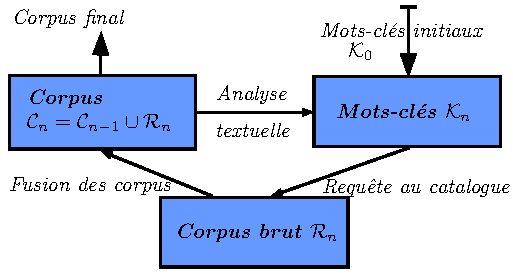
\includegraphics[width=0.8\linewidth]{Figures/QuantEpistemo/schema_algo}
\caption[Systematic review algorithm workflow][Algorithme de revue systématique]{Global workflow of the algorithm, including implementation details: catalog request is done through Mendeley API; final state of corpuses are RIS files.\label{fig:quantepistemo:algo}}{Architecture globale de l'algorithme, incluant des détails d'implémentation : la requête au catalogue est faite via l'API Mendeley \comment[FL]{tu ne l'as pas dit auparavant}; les corpus finaux sont sous forme de fichiers RIS.\label{fig:quantepistemo:algo}\comment[FL]{traduire ; pourquoi mendeley ?}}
\end{figure}
%%%%%%%%%%%%%%%%%%%%%%%%%%%%



%%%%%%%%%%%%%%%%%%%%%%%%%%%%
\paragraph{Results}{Résultats}



\bpar{
Once the algorithm is partially validated, we apply it to our question. We start from five different initial requests that were manually extracted from the various domains identified in the bibliography (that are ``city system network'', ``land use transport interaction'', ``network urban modeling'', ``population density transport'', ``transportation network urban growth''). We take the weakest assumption on parameter $N_k=100$, as it should less constrain reached domains. After having constructed corpuses, we study their lexical distances as an indicator to answer our initial question. Large distances would go in the direction of the assumption made above, i.e. that discipline self-centering may be at the origin of the lack of interest for co-evolutive models. We show in Table~\ref{tab:quantepistemo:lexical} values of relative lexical proximity, that appear to be significantly low, confirming this assumption.
}{
Les détails précis concernant l'implémentation de l'algorithme ainsi qu'une analyse de sensibilité pour vérifier la convergence sur un échantillon de requêtes initiales (typiques des champs étudiés\comment[FL]{?}) sont donnés en Appendice~\ref{app:sec:quantepistemo}. Lorsque l'algorithme a été partiellement validé par cette analyse, nous l'appliquons à notre question.\comment[AB]{a revoir} Nous partons de cinq différentes requêtes initiales qui ont été manuellement extraites des divers domaines identifiés dans la bibliographie (qui sont ``city system network'', ``land use transport interaction'', ``network urban modeling'', ``population density transport'', ``transportation network urban growth'')\comment[FL]{ces mots sont nombreux, quel impact sur l'algo ?}\comment[FL]{du coup tu exclues totalement la literature francophone. pourquoi ce choix ?}\footnote{Ce choix est arbitraire,\comment[FL]{on espere que non} cette étude étant préliminaire on admet de travailler potentiellement sur des échantillons. Par exemple, l'utilisation de ``co-evolution'' n'est pas concluante car trop peu d'articles utilisent cette formulation.}. Nous prenons l'hypothèse la plus faible pour le paramètre $N_k=100$ (plus $N_k$ est grand, plus les domaines atteints devraient être moins restreints et donc plus des résultats de distance seront significatifs)\comment[FL]{phrase non comprehensible}. Après avoir construit les corpus, nous étudions leur cohérence lexicale comme un indicateur de réponse à notre question initiale. De grande distances devraient confirmer l'hypothèse formulée ci-dessus, i.e. que des disciplines auto-centrées pourraient être à l'origine d'un manque d'intérêt pour des modèles co-évolutifs. La table~\ref{tab:quantepistemo:lexical} montre les valeurs\comment[FL]{tu n'as pas explique comment tu quantifies cela} de la proximité lexicale relative, qui est significativement faibles\comment[FL]{sens ?} sachant que les chiffres peuvent directement s'interpréter comme une proportion de mots en co-occurrence, ce qui tend à confirmer notre hypothèse. Pour situer ces résultats de manière relative, il faudrait un modèle nul\comment[FL]{?} avec des corpus aléatoires par exemple, ce qui pourrait faire l'objet de développements futurs. 
}




%%%%%%%%%%%%%%%%%%%%%%%%%%%%
\begin{table}
\caption[Stationary lexical proximities][Proximités lexicales stationnaires]{Symmetric matrix of lexical proximities between final corpuses, defined as the sum of overall final keywords co-occurrences between corpuses, normalized by number of final keywords (100). We obtain very low values, confirming that corpuses are significantly far. Size of final corpuses is given as $W$.\label{tab:quantepistemo:lexical}}{Matrice symétrique des proximités lexicales entre les corpus finaux, définies comme la somme des co-occurrences totale de mots-clés finaux entre corpus, normalisé par le nombre de mots-clés finaux (100). La taille des corpus finaux est donnée par $W$. Les valeurs obtenues pour les proximités sont considérablement faibles, ce qui confirme que les corpus sont éloignés de manière significative (voir texte).\comment[FL]{ce tableau est difficilement comprehensible ; traduire ; trop de chiffres significatifs.}\comment[AB]{C’est vrai que sans valeurs de références c’est difficile à interpréter. Quelle serait la valeur max pour un corpus de taille X et un nombre de mots clés Y ?}\label{tab:quantepistemo:lexical}}
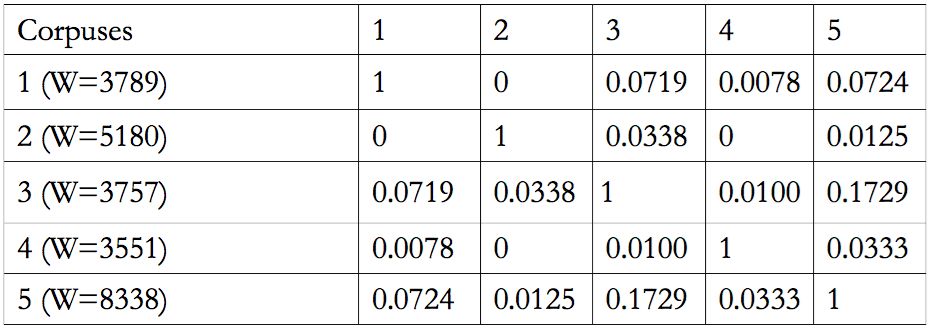
\includegraphics[width=0.8\linewidth]{Figures/QuantEpistemo/corpusesDistances}
\end{table}
%%%%%%%%%%%%%%%%%%%%%%%%%%%%




\bpar{
Possible developments can include the construction of citation networks through an automatic access to Google Scholar that provides backward citations. The confrontation of inter-cluster coefficients on the citation network for the different corpuses with lexical consistence are an essential aspect of a further validation of our results.
}{
Les développements possibles incluent la construction de réseaux de citation via un accès automatique à Google Scholar\comment[FL]{pourquoi cette plateforme et pas une autre ?} \comment[AB]{c’est ton unique source ?
Si je fais une recherche à la main dans google scholar avec les termes « urban growth networks » j’obtiens des références, par exemple 
Streets tree networks and urban growth: optimal geometry for quickest access between a finite-size volume and one point
A Bejan, GA Ledezma - Physica A: Statistical Mechanics and its …, 1998} qui fournit les citations entrantes. La confrontation des coefficients inter-clusters pour le réseau de citations entre les différents corpus avec la cohérence lexicale est un aspect clé d'une validation approfondie des résultats.
}



\bpar{
The disturbing absence of models simulating the co-evolution of transportation networks and urban land-use, confirmed through a state-of-the-art covering many domain, may be due to the absence of communication between scientific disciplines studying different aspects of that problems. We have proposed an algorithmic method to give elements of answers through text-mining-based corpus extraction. First numerical results seem to confirm the assumption. However, such a quantitative analysis should not be considered alone, but rather come as a back-up for qualitative studies that will be the object of further work, such as the one lead in~\cite{commenges:tel-00923682}, in which questionnaires with historical actors of modeling provide highly relevant information.
}{
L'absence peu explicable\comment[FL]{pourquoi cette hypothese ?} \comment[AB]{qu’entends tu par « absence » de modèles ?} a priori de modèles qui simulent la co-évolution des réseaux de transport et de l'usage du sol urbain, qui se confirme à première vue par un état de l'art couvrant des domaines disparates, pourrait être due à l'absence de communication entre les disciplines scientifiques étudiant différents aspects du problème. D'autres explications possibles qui en sont proches peuvent par exemple être le manque de cas d'application concrets de tels modèles vu les échelles temporelles mises en jeu et donc l'absence de financement propre - ce qui n'est pas si loin de l'absence d'une discipline y consacrant certains de ses objets. Cette question des portées et des échelles des modèles fera l'objet de la meta-analyse à la section suivante~\ref{sec:modelography}. Ainsi, nous avons proposé ici une méthode algorithmique pour donner des éléments de réponse par l'extraction de corpus basée sur l'analyse textuelle. Les premiers résultats numériques semblent confirmer l'hypothèse\comment[AB]{laquelle ?}. Cependant, une telle analyse quantitative ne doit pas être considérée seule, mais devrait plutôt venir comme soutien à des études qualitatives qui peuvent être l'objet de développements futurs, comme celle menée dans~\cite{commenges:tel-00923682}, dans laquelle des questionnaires avec des acteurs historiques fournit des informations extrêmement pertinentes. \comment[FL]{ET A UNE REVUE DE BIBLIO CLASSIQUE}[(JR) faite en 2.1]
}




%--------------------------------------------------------------


%%%%%%%%%%%%%%%%%%%%%%%%
%\subsection[Indirect Bibliometrics][Bibliométrie indirecte]{Indirect bibliometrics through Complex Network analysis}{Bibliométrie Indirecte par Analyse de Réseaux Complexes}
\subsection{Indirect Bibliometrics}{Bibliométrie indirecte}

\label{subsec:indirectbibliometrics}


\bpar{
As described before, semantic analysis of final corpus does not contain all the information on disciplinary compartmentation nor on patterns of propagation of scientific knowledge as the ones contained in citation networks for example. Furthermore, data collection in the previous algorithm is subject to convergence towards self-consistent themes because of the proper structure of the method. It may give more insight about scientific social patterns of ontological choices in modeling to study communities in broader networks, that would more correspond to disciplines (or sub-disciplines depending on granularity level). We propose to reconstruct disciplines around our thematic, to obtain a more precise view of interdisciplinarity and the scientific landscape on our subject.
}{
Comme décrit précédemment, l'analyse sémantique des corpus finaux ne contient pas la totalité de l'information sur les liens entre disciplines ni sur les motifs de propagation de la connaissance scientifique comme ceux contenus dans les réseaux de citations par exemple. De plus, la collection des données dans l'algorithme précédent est sujette à convergence vers des thèmes relativement auto-cohérents de par la structure propre de la méthode. On pourrait obtenir plus d'information sur les motifs sociaux de choix ontologiques\comment[FL]{sens ?} pour la modélisation en étudiant les communautés dans des réseaux plus larges, ce qui correspondrait plus à des disciplines (ou des sous-disciplines selon le niveau de granularité). Nous proposons de reconstruire les disciplines autour de notre thématique, pour obtenir une vue plus précise de l'interdisciplinarité\comment[FL]{est ce que si les disciplines sont (re) construites par l'algo, la notion d'interdisciplinarite a le meme sens ?} et du paysage scientifique sur notre sujet. 
}


\subsubsection{Context}{Contexte}


\bpar{
Most of scientific disciplines seem to be in a need of more interdisciplinarity and transversal approaches, as highlighted by the special issue of Nature (\cite{natureInterdisc}), for diverse reasons that may include the development of vertically integrated fields conjointly with horizontal questions as detailed in the Complex Systems roadmap (\cite{2009arXiv0907.2221B}). There are naturally ongoing debates on what is exactly interdisciplinarity (many other terms such as trans-disciplinarity, cross-disciplinarity also exist) and it actually depends of involved domains : recent hybrid disciplines (see e.g. the ones underlined  by \cite{bais2010praise} such as astro-biology) are a good illustration of the case where entanglement is strong and new discoveries are vertically deep, whereas more loose fields such as ``urbanism'' which has no precise definition and integration is by essence horizontal is an other illustration of how transversal knowledge can be produced (leading to misunderstandings when recently introduced to non-aware physicists as warned by~\cite{dupuy2015sciences}). This question projects itself naturally into the field of scientific communication : what are corresponding alternatives for an efficient dissemination of knowledge ? Elements of answer to such a high-level issue imply, in an evidence-based perspective, quantitative measures of interdisciplinarity, that would be part of a multidimensional approach of the study of science that is in a way ``beyond bibliometrics'' (\cite{cronin2014beyond}).
}{
La majorité des disciplines scientifiques présentent un besoin\comment[FL]{n'y a t'il pas la deja un postulat fort ?} fort en interdisciplinarité et approches transversales, comme illustré par exemple par l'édition spéciale récente de Nature sur le sujet (\cite{natureInterdisc}), pour diverses raisons qui peuvent inclure le développement de champs intégrés verticalement\comment[FL]{sens ?} conjointement aux questions horizontales comme détaillé dans la feuille de route des Systèmes Complexes \comment[FL]{expression grandiloquente}[(JR) pas d'autre facon de nommer la roadmap](\cite{2009arXiv0907.2221B}). Les débats courants sur la nature exacte de l'interdisciplinarité sont bien sûr nombreux (d'autres termes existent comme transdisciplinarité ou cross-disciplinarité), et celle-ci dépend en fait des domaines impliqués : des disciplines hybrides apparues récemment (voir par exemples celles soulignées par \cite{bais2010praise} comme l'astro-biologie \comment[FL]{la geomatique}) sont une bonne illustration du cas où les intrications sont très fortes, tandis que des champs plus mou\comment[FL]{mauvaise strategie je pense : avant de designer une discipline en particulier, il faut preciser le sens de ``mou''} comme ``l'urbanisme'' qui n'ont pas de définition précise\comment[FL]{mal dit} montrent comment l'intégration horizontale est nécessaire et comment de la connaissance transversale peut être produite (menant à des possibles malentendus\comment[FL]{et alors ? est ce que les malentendus sont necessairement contre-productifs ?} lorsque récemment introduite trop brutalement à des physiciens comme montré par~\cite{dupuy2015sciences}). Cette question se transfère naturellement au champ de la communication scientifique : quelles sont les alternatives correspondantes pour une dissémination efficace de la connaissance ? Des éléments de réponse à une question si générale impliquent, dans une perspective \emph{evidence-based}\comment[FL]{traduire}[(JR)non traduisible - appuyer quelque part sur le sens de l'evidence-based], des mesures quantitatives de l'interdisciplinarité, qui font partie d'une approche multi-dimensionnelle de l'étude de la science, en quelque sorte ``au-delà de la bibliométrie''~\cite{cronin2014beyond}\comment[FL]{que tu n'as pas introduite}.
}


\bpar{
The possible methods for quantitative insights into epistemology are numerous. Using citation network features, a good predicting power for citation patterns is for example obtained by~\cite{2013arXiv1310.8220N}. Co-authorship networks can also be used for predictive models (\cite{2014arXiv1402.7268S}). A multilayer network approach was recently proposed in~\cite{2016arXiv160106075O}, using bipartites networks of papers and scholars, in order to produce measures of interdisciplinarity. Disciplines can be stratified into layers to reveal communities between them and therein collaboration patterns (\cite{2015arXiv150601280B}). Keyword networks are used in other fields such as economics of innovation: for example, \cite{choi2014patent} proposes a method to identify technological opportunities by detecting important keywords from the point of view of topological measures. \cite{shibata2008detecting} uses topological analysis of the citation network to detect emerging research fronts.
}{
Les méthodes potentielles pour des entrées quantitatives en épistémologie sont nombreuses. En utilisant les caractéristiques des réseaux de citation, un bon pouvoir prédictif pour les motifs de citation est par exemple obtenu par~\cite{2013arXiv1310.8220N}. Les réseaux de co-auteurs peuvent également être utilisés pour des modèles prédictifs~\cite{2014arXiv1402.7268S}. Une approche multi-couches a récemment été proposée par~\cite{2016arXiv160106075O}, utilisant des réseaux bipartites des papiers et des chercheurs, dans le but de produire des mesures d'interdisciplinarité. Les disciplines peuvent être stratifiées en couches pour révéler des communautés entre elles et ainsi des motifs de collaboration~\cite{2015arXiv150601280B}. Les réseaux de mots-clés sont utilisés dans d'autres champs comme l'économie de l'innovation : par exemple, \cite{choi2014patent} introduit une méthode pour identifier les opportunités technologiques en détectant des mots-clés importants au sens des mesures topologiques. \cite{shibata2008detecting} utilise l'analyse topologique du réseau de citations pour détecter des fronts de recherche émergents.
}

\bpar{
The approach developed here couples citation network exploration and analysis with text-mining, aiming at mapping the scientific landscape in the neighborhood of a particular corpus. The context is particularly interesting for the methodology developed. First of all, the subject studied is very broad and by essence interdisciplinary. Secondly, bibliographical data is difficult to obtain, raising the concern of how the perception of a scientific landscape may be shaped by actors of the dissemination and thus far from objective, making technical solutions as the ones consequently developed here crucial tools for an open and neutral science. Our approach combine semantic communities analysis (as done in~\cite{2016arXiv160208451P} for papers in physics but with keyword extraction ; \cite{2015arXiv151003797G} analyses semantic networks of political debates) with citation network to extract e.g. interdisciplinarity measures. Our contribution differs from the previous works quantifying interdisciplinarity as it does not assume predefined domains nor classification of the considered papers, but reconstructs from the bottom-up the fields with the endogenous semantic information. \cite{nichols2014topic} already introduced a close approach, using Latent Dirichlet Allocation topic modeling to characterize interdisciplinarity of awards in particular sciences. \cite{lariviere201410} quantifies interdisciplinarity over a long time range by looking at the field of references of publications.
}{
L'approche développée ici couple exploration et analyse de réseau de citation avec analyse textuelle, dans le but de cartographier le paysage scientifique dans le voisinage d'un corpus donné. Le contexte est particulièrement intéressant pour la méthodologie développée. Premièrement, le sujet étudié est très large et par essence interdisciplinaire. Deuxièmement, les données bibliographiques sont difficiles à obtenir, soulevant la question de comment la perception d'un horizon scientifique peut être déterminée par les acteurs de la dissémination et donc loin d'être objective, rendant les solutions techniques comme celle développée ici en conséquence des outils cruciaux pour une science ouverte et neutre. Notre approche combine une analyse des communautés sémantiques (comme fait dans~\cite{2016arXiv160208451P} pour les articles en physique mais sans extraction des mots-clés, ou par \cite{2015arXiv151003797G} pour un analyse des réseaux sémantiques de débats politiques) avec celle du réseau de citations pour extraire par exemple des mesures d'interdisciplinarité. Notre contribution se démarque des travaux précédents quantifiant l'interdisciplinarité puisqu'elle ne suppose pas de domaines a priori ou une classification des références considérées, mais reconstruit par le bas les champs via l'information sémantique endogène. \cite{nichols2014topic} introduit une approche similaire, utilisant le modèle d'extraction de thématiques \emph{Latent Dirichlet Allocation}\footnote{Le modèle LDA, introduit par~\cite{blei2003latent}, suppose les documents comme produits par des thèmes sous-jacents, avec une distribution de Dirichlet pour leur composition ainsi que pour la distribution des mots par thèmes. Son estimation donne la composition des thèmes en terme de mots-clés.} pour caractériser l'interdisciplinarité de récompenses dans des sciences précises. \cite{lariviere201410} quantifie l'interdisciplinarité sur une longue période temporelle en étudiant l'étendue de la bibliographie des publications.\comment[FL]{vague}
}



%%%%%%%%%%%%%%%%%%%%%%%
\subsubsection{Database Construction}{Données}


\bpar{
Our approach imposes some requirements on the dataset used, namely: (i) cover a certain neighborhood of the studied journal in the citation network in order to have a consistent view on the scientific landscape; (ii) have at least a textual description for each node. For these to be met, we need to gather and compile data from heterogeneous sources, using therefore a specific application, which general architecture is synthesized in Fig.~\ref{fig:datacollection}. For the sake of simplicity, we will denote by \emph{reference} any standard scientific production that can be cited by another (journal paper, book, book chapter, conference paper, communication, etc.) and contains basic records (title, abstract, authors, publication year). We will work in the following on networks of references. Note that one significant contribution of this paper is the construction of such an hybrid dataset from heterogeneous sources, and the development of associated tools that can be reused and further developed for similar purposes.
}{
Notre approche implique des spécifications pour le jeu de données utilisé, à savoir : (i) couvrir un voisinage conséquent du corpus étudié dans le réseau de citation afin d'avoir une vue la moins biaisée possible du paysage scientifique ; (ii) avoir au moins une description textuelle pour chaque noeud.\comment[FL]{B} Pour cela, nous rassemblons et compilons les données de sources hétérogènes en utilisant une architecture et implémentation spécifiques, décrites en Appendice~\ref{app:sec:cybergeo}. Pour simplifier, nous dénommons \emph{référence} toute production scientifique standard\footnote{ce qui est bien sûr sujet à débat, voir nos discussions en ouverture sur l'évolution des modes de communication scientifique} qui peut être citée par une autre (articles de journaux, livre, chapitre de livre, article d'actes, communication, etc.) et contient des informations de base (titre, résumé, auteurs, année de publication). Nous travaillons par la suite sur le réseau des références. Il est important de noter qu'une contribution fondamentale\comment[FL]{le dire avant} de cette partie consiste en la construction de jeux de données hybrides à partir de sources hétérogènes, et les développement des outils associés qui peuvent être réutilisés et améliorés pour des applications similaires.
}

\paragraph{Initial Corpus}{Corpus Initial}

Notre corpus initial est construit à partir de l'état de l'art établi en~\ref{sec:modelingsa}. Sa composition complète est donnée en Appendice~\ref{app:sec:quantepistemo}. Celui-ci est pris de taille raisonnable\comment[FL]{sens ?}, mais les méthodes utilisées ici ont été développées sur des données massives, pour les brevets par exemple~\cite{bergeaud2017classifying}.


\paragraph{Citation Data}{Données de citation}

\bpar{
Citation data is collected from \texttt{Google Scholar}\comment[FL]{police}, that is the only source for incoming citations~\cite{noruzi2005google} in our case as the journal is poorly in other databases\footnote{or was just added as in the case of \textit{Web of Science}, indexing \textit{Cybergeo} since May 2016}. We are aware of the possible biaises using this single source (see e.g.~\cite{bohannon2014scientific})\footnote{or \texttt{http:\/\/iscpif.fr\/blog\/2016\/02\/the-strange-arithmetic-of-google-scholars}}, but these critics are more directed towards search results than citation counts. %The automatic collection requires the use of an open source data crawling software to pipe requests, namely \texttt{TorPool}~\cite{torpool} that provides a Java API allowing an easy integration into our application. Using it, a crawler can retrieve html pages and get backward citation data, i.e. all citing articles for a given initial article.
 We retrieve that way two sub-corpuses: references \emph{citing} Cybergeo and references \emph{citing the ones cited} by cybergeo. At this stage, the full corpus contains around $4\cdot10^5$ references.
}{
Le réseau de citations est reconstruit à partir de \texttt{Google Scholar} qui est souvent l'unique source des citations entrantes~\cite{noruzi2005google} puisqu'en science humaines les ouvrages ne sont pas systématiquement référencés par les bases fournissant des services (payants) comme le réseau de citation.\footnote{Par exemple, le journal Cybergeo n'est indexé dans le \emph{Web of Science} que depuis mai 2016, suite à des négociations ardues et non sans contrepartie.} Nous sommes conscient des biais possibles de l'utilisation de cette source unique (voir par exemple~\cite{bohannon2014scientific})\footnote{ou \texttt{http:\/\/iscpif.fr\/blog\/2016\/02\/the-strange-arithmetic-of-google-scholars}}, mais ces critiques sont dirigées vers les résultats de recherche plutôt que les comptes de citations. Nous récoltons ainsi les références \emph{citantes} à profondeur deux, c'est à dire les références citant le corpus initial et celles citant celles-ci. Le réseau obtenu contient $V=9462$ références correspondant à $E=12004$ liens de citation. Concernant les langues, l'anglais représente 87\% du corpus, le français 6\%, l'espagnol 3\%, l'allemand 1\%, complété par des langues comme le mandarin pouvant être indéfinies (la détection de celui-ci étant peu fiable). Le corpus n'est pas très international (contrairement par exemple au thème de la croissance urbaine, étudié pour le développement thématique sur les liens entre économie et géographie développé en~\ref{app:sec:ecogeo}).
}

\paragraph{Text Data}{Données textuelles}

\bpar{
A textual description for all references is necessary for a complete semantic analysis. We use for this an other source of data, that is the online catalog of \textit{Mendeley} reference manager software~\cite{mendeley}. It provides a free API allowing to get various records under a structured format. Although not complete, the catalog provides a reasonable coverage (over 55\%), yielding a final corpus with full abstracts of size $2.1\cdot 10^5$, which structure is recalled in Fig.~\ref{fig:citationnetwork}
}{
Pour mener l'analyse sémantique, une description suffisamment conséquente est nécessaire. Nous collectons pour cela les résumés pour le réseau précédent. Ceux-ci sont disponibles pour environ un tiers des références, donnant $V=3510$ noeuds avec description textuelle.
}



%%%%%%%%%%%%%%%%%%
\subsubsection{Results}{Résultats}


\paragraph{Citation Network Properties}{Réseau de citations}


Des statistiques basiques pour le réseau de citation donnent déjà des informations intéressantes. Le réseau a un degré moyen de $\bar{d}=2.53$ et une densité de $\gamma=0.0013$\comment[AB]{comparer avec des valeurs de référence ?}. Le degré entrant moyen (qui peut être interprété comme un facteur d'impact stationnaire) est de 1.26, ce qui est relativement élevé pour des sciences humaines. Il est important de noter sa connexité faible, ce qui signifie que les domaines initiaux ne sont pas en isolation totale : les références initiales sont partagées à un degré minimal par les différents domaines. Nous travaillons sur la suite sur le sous-réseau des noeuds comprenant au moins deux liens, pour extraire le coeur de la structure du réseau et se débarrasser de l'effet ``grappe''. De plus, le réseau est nécessairement complet entre ces noeuds puisqu'on est remonté au deuxième niveau. Nous procédons à une détection de communautés par l'algorithme de Louvain, sur le réseau non-dirigé correspondant. On obtient 13 communautés\comment[FL]{comment ? c'est elliptique}[(JR) dit juste avant, algo de Louvain], de modularité dirigée 0.66, extrêmement significative en comparaison à une estimation par bootstrap de la même mesure sur le graphe aléatoirement rebranché qui donne une modularité de $0.0005 \pm 0.0051$ sur $N=100$ répétitions. Les communautés font sens de manière thématique, puisqu'on retrouve pour les plus grosses les domaines suivants : LUTI (18\% du réseau), Géographie Urbaine et des Transports (16\%), Planification des infrastructures (12\%), Planification intégrée - TOD (6\%), Réseaux Spatiaux (17\%), Etudes d'accessibilité (18\%).\comment[FL]{quelle est leur coherence interne ? comment as tu donne les noms ?}[(JR) cf remarque de Caruso a ECTQG] La Fig.~\ref{fig:quantepistemo:citnw} permet de visualiser les relations de ces domaines. Il est intéressant d'observer que les travaux des économistes et des physiciens dans le domaine tombent dans la même catégorie d'étude des \emph{Spatial Networks}. En effet, la littérature citée par les physiciens comporte souvent plus d'ouvrage en économie qu'en géographie, tandis que les économistes utilisent des techniques d'analyse de réseau. Ensuite, le planning, l'accessibilité, les LUTI et le TOD sont très proches mais se distinguent dans leur spécificités: le fait qu'ils apparaissent dans des communautés séparées est un résultat en lui-même témoignant d'une certaine séparation.\comment[FL]{phrase alambiquee} Ceux-ci font le pont entre les approches Réseaux spatiaux et les approches géographiques, qui comportent une partie importante de sciences politiques par exemple. Les liens entre physique et géographie restent très faibles. Ce panorama dépend bien sûr du corpus initial, mais nous permet de mieux comprendre le contexte de celui-ci dans son environnement disciplinaire.


%%%%%%%%%%%%%%%%%
\begin{figure}[!ht]
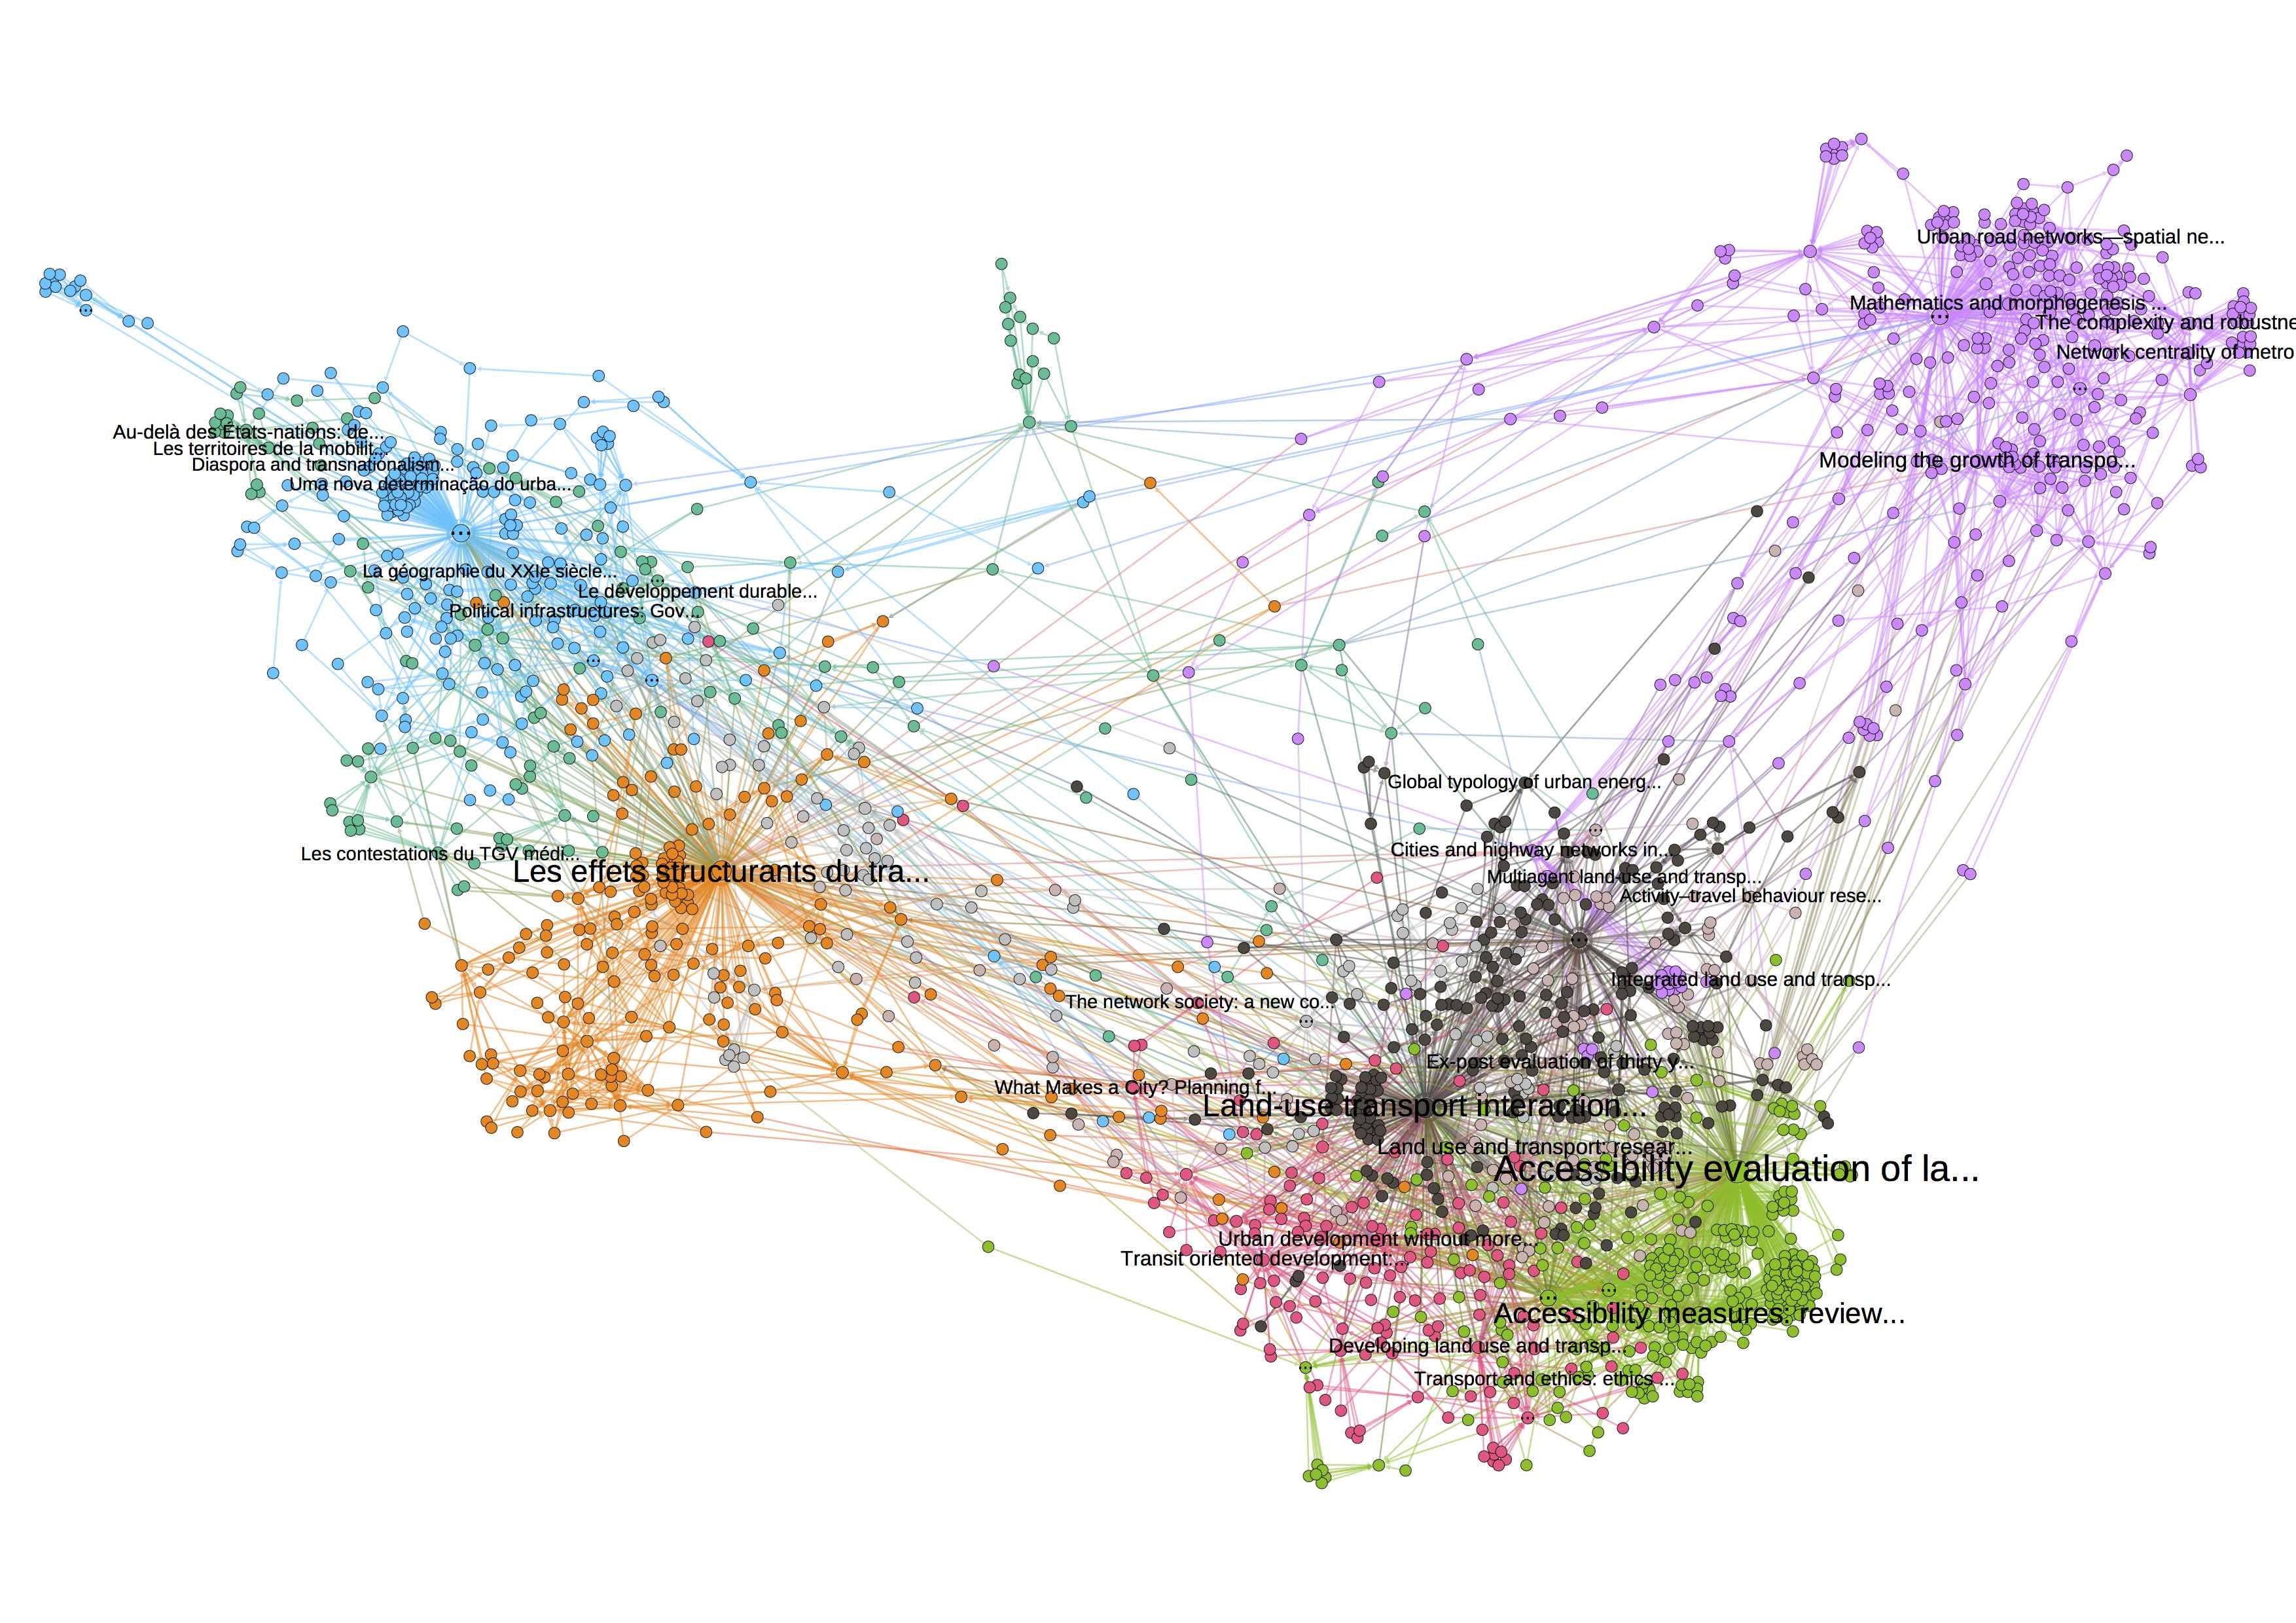
\includegraphics[width=\linewidth]{Figures/QuantEpistemo/rawcore}
\caption[Citation Network][Réseau de citations]{\textbf{Citation Network}\label{fig:quantepistemo:citnw}}{\textbf{Réseau de citations.} Nous visualisons les références ayant au moins deux liens, par un algorithme de force-atlas. Les couleurs donnent les communautés décrites dans le texte. En orange, bleu, turquoise: géographie urbaine, géographie des transports, sciences politiques ; en rose, noir, vert: planning, accessibilité, LUTI ; en violet : réseaux spatiaux (physique et économie).\label{fig:quantepistemo:citnw}}
\end{figure}
%%%%%%%%%%%%%%%%%





%%%%%%%%%%%%%%%%%%
\paragraph{Semantic Communities}{Communautés Sémantiques}


L'extraction des mots-clés est faite suivant une heuristique inspirée de~\cite{chavalarias2013phylomemetic}. La description complète de la méthode et de son implémentation est donnée en Appendice~\ref{app:sec:cybergeo}. Elle se base sur les relations au second ordre entre les entités sémantiques, qui sont des \emph{n-grams}, c'est à dire des mots-clés multiples pouvant avoir une longueur jusqu'à 3. Celles-ci sont estimées via la matrice de co-occurrence, dont les propriétés statistiques fournissent une mesure de déviation à des co-occurrences uniformes, qui est utilisée pour juger la pertinence des mots-clés. Sélectionnant un nombre fixe de mots-clés pertinents $K_W = 10000$, nous pouvons ensuite construire un réseau pondéré par les co-occurrences.


\bpar{
The topology of raw networks does not allow the extraction of clear communities, in particular because of the presence of hubs that correspond to frequent terms common to many fields (e.g. \texttt{model}, \texttt{space}). We assume these highest degree terms do not carry specific information on particular classes and can be thus filtered given a maximal degree threshold $k_{max}$. Similarly, edge with small weight are considered as noise and filtered according to a minimal edge weight threshold $\theta_w$. Keywords are preliminary filtered by a document frequency window $\left[ f_{min},f_{max} \right]$ which is slightly different from network filtering and complementary. A sensitivity analysis of resulting network topology to these parameters is presented in Fig.~\ref{fig:sensitivity}. We choose parameter values that maximize modularity under the constraint of a community number and size distribution of same magnitude as technological classes. This multi-objective optimization does not have a unique solution as objectives are somehow contradictory, and a compromise point must be chosen.
}{
La topologie du réseau brut ne permet pas l'extraction claire de communautés, en particulier à cause de hubs qui correspondent à des termes fréquents commun à de nombreux champs (e.g. \texttt{model}, \texttt{space})\comment[FL]{statut de ces mots ?}. Nous faisons l'hypothèse que ces termes à fort degré ne portent pas d'information particulière sur des classes données et peuvent ainsi être filtrés étant donné un seuil de degré maximal $k_{max}$ (on s'intéresse alors à ce qui fait la spécificité de chaque domaine). De la même manière, les liens avec un poids faibles sont considérés comme du bruit et filtrés selon un seuil de poids minimal $\theta_w$. La méthode générique permet de plus une filtration préliminaire des mot-clés, complémentaire à la filtration topologique, par fréquence d'apparition dans les documents $\left[ f_{min},f_{max} \right]$, à laquelle les résultats ne sont pas sensibles dans notre cas. L'analyse de sensibilité des caractéristiques du réseau filtré, notamment de sa taille, modularité et structure des communautés, est donnée en~\ref{app:sec:quantepistemo}. Nous choisissons des valeurs de paramètres permettant une optimisation multi-objectifs entre modularité et taille du réseau, $\theta_w = 10,k_{max} = 500$, par le choix d'un point compromis sur un front de Pareto, qui donne un réseau sémantique de taille $(V=7063,E=48952)$. Celui-ci est visualisé en Appendice~\ref{app:sec:quantepistemo}.
}


\bpar{
We then retrieve communities in the semantic network (using standard Louvain algorithm, with the optimized filtering parameters). communities correspond to well-defined scientific fields (and/or domains, approaches). An expert validation allow us to give names to these, a more complicated naming procedure would eventually be possible (as in~\cite{yang2000improving} for the case of patents 
 where a chi-square test on distribution of documents in classes), but we prefer to stick here to a certain level of supervision. Table~\ref{tab:domains} summarizes the communities 
}{
Nous récupérons ensuite les communautés dans le réseau par un clustering de Louvain standard sur le réseau filtré optimal. On obtient 20 communautés pour une modularité de 0.58. Celles-ci sont examinées à la main pour être nommées, les techniques de désignation automatique~\cite{yang2000improving} ne sont pas assez élaborées pour faire la distinction implicite entre champs thématiques et méthodologiques par exemple (en fait entre les domaines de connaissance, voir~\ref{sec:knowledgeframework}) qui est une dimension supplémentaire que nous ne traitons pas ici, mais nécessaire pour avoir des désignations parlantes. Les communautés sont décrites en Table~\ref{tab:quantepistemo:semanticdomains}. On voit tout de suite la complémentarité avec l'approche par citations, puisque se dégagent ici à la fois des sujet d'étude (High Speed Rail, Maritime Networks), des domaines et méthodes (Networks, Remote Sensing, Mobility Data Mining), des domaines thématiques (Policy), des méthodes pures (Agent-based Modeling, Measuring). Ainsi, une référence peut mobiliser plusieurs de ces communautés. On a de plus une granularité plus fine de l'information. L'effet du langage est puissant puisque la géographie française se distingue en une catégorie séparée (des analyses poussées pourraient être envisagées pour mieux comprendre le phénomène et en tirer parti: sous-communautés, reconstruction d'un réseau spécifique, études par traduction ; mais celles-ci sont hors de propos dans cette étude exploratoire). On constante l'importance des réseaux, des problématiques de sciences politiques et socio-économiques. Nous mobiliserons la première catégorie dans la plupart des modèles développés, mais en gardant en tête l'importance des problématiques liées à la gouvernance, nous réaliserons un travail spécifique en~\ref{sec:lutetia}.
}




%%%%%%%%%%%%%%%%%%
\begin{table}
\caption[Semantic communities][Communautés sémantiques]{Disciplines/domains/fields reconstructed from community detection in the semantic network}{\textbf{Description des communautés sémantiques.} On donne leur taille, leur proportion en quantité de mots-clés cumulés sur l'ensemble du corpus, et des mots-clés représentatifs sélectionnés par degré maximal.\comment[FL]{pourquoi ces mots sont ils tronques ?}[(JR) cest explique dans le texte (surtout en annexe) il s'agit de stem]\label{tab:quantepistemo:semanticdomains}}
\begin{tabular}{llll}
\hline\noalign{\smallskip}
Name & Size & Weight & Keywords  \\
\noalign{\smallskip}\hline\noalign{\smallskip}
Networks & 820 & 13.57\% & \texttt{social network, spatial network, resili} \\
Policy & 700 & 11.8\% & \texttt{actor, decision-mak, societi} \\
Socio-economic & 793 & 11.6\% & \texttt{neighborhood, incom, live} \\
High Speed Rail & 476 & 7.14\% & \texttt{high-spe, corridor, hsr} \\
French Geography & 210 & 6.08\% & \texttt{système, développement, territoire} \\
Education & 374 & 5.43\% & \texttt{school, student, collabor} \\
Climate Change & 411 & 5.42\% & \texttt{mitig, carbon, consumpt} \\
Remote Sensing & 405 & 4.65\% & \texttt{classif, detect, cover} \\
Sustainable Transport & 370 & 4.38\% & \texttt{sustain urban, travel demand, activity-bas} \\
Traffic & 368 & 4.23\% & \texttt{traffic congest, cbd, capit} \\
Maritime Networks & 402 & 4.2\% & \texttt{govern model, seaport, port author} \\
Environment & 289 & 3.79\% & \texttt{ecosystem servic, regul, settlement} \\
Accessibility & 260 & 3.23\% & \texttt{access measur, transport access, urban growth} \\
Agent-based Modeling & 192 & 3.18\% & \texttt{agent-bas, spread, heterogen} \\
Transportation planning & 192 & 3.18\% & \texttt{transport project, option, cba} \\
Mobility Data Mining & 168 & 2.49\% & \texttt{human mobil, movement, mobil phone} \\
Health Geography & 196 & 2.49\% & \texttt{healthcar, inequ, exclus} \\
Freight and Logistics & 239 & 2.06\% & \texttt{freight transport, citi logist, modal} \\
Spanish Geography & 106 & 1.26\% & \texttt{movilidad urbana, criteria, para} \\
Measuring & 166 & 1.0\% & \texttt{score, sampl, metric} \\
\noalign{\smallskip}\hline
\end{tabular}
\end{table}
%%%%%%%%%%%%%%%%%%



%%%%%%%%%%%%%%%%%%
\paragraph{Measures of Interdisciplinarity}{Mesures d'interdisciplinarité}


\bpar{
Distribution of keywords within communities provides an article-level interdisciplinarity.
Combination of citation and semantic layers in the hyper-network provide second order interdisciplinarity measures, that we don't use here because of the modest size of the citation network. More precisely, a reference can be viewed as a probability vector on semantic classes.
}{
La distribution des mots clés dans les communautés permettent de définir une mesure d'interdisciplinarité au niveau de l'article. La combinaison des couches de citation et sémantique dans l'hyperréseau fournit des mesures d'interdisciplinarité au second ordre (motifs sémantiques des cités ou des citants), que nous n'utiliserons pas ici à cause de la taille modeste du réseau de citation (voir \ref{app:sec:cybergeo} et \ref{app:sec:patents}). Plus précisément, une référence $i$ peut être vue comme un vecteur de probabilités sur les classes sémantiques $j$, qu'on notera sous forme matricielle $\mathbf{P}=(p_{ij})$. Celles-ci sont estimées simplement par les proportions de mots-clés classifiés dans chaque classe pour la référence. Une mesure classique d'interdisciplinarité~\cite{bergeaud2017classifying} est alors $I_i = 1 - \sum_j p_{ij}^2$. Soit $\mathbf{A}$ la matrice d'adjacence du réseau de citation, et soit $\mathbf{I}_k$ les matrices de selection des lignes correspondants à la classe $k$ de la classification de citation: $Id\cdot \mathbbm{1}_{c(i)=k}$, telle que $I_k \cdot A \cdot I_{k'}$ donne exactement les citations de $k$ vers $k'$. La proximité de citation entre les communautés de citation est alors définie par $c_{kk'} = \sum \mathbf{I}_k \cdot \mathbf{A} \cdot \mathbf{I}_{k'} /  \sum \mathbf{I}_k \cdot \mathbf{A}$. On définit la proximité sémantique en définissant une matrice de distance entre références par $\mathbf{D} = d_{ii'}=\sqrt{\frac{1}{2}\sum (p_{ij}-p{i'j})^2}$ puis la proximité sémantique par $s_{kk'} = \mathbf{I}_k \cdot \mathbf{D} \cdot \mathbf{I}_{k'} / \sum \mathbf{I}_k \sum \mathbf{I}_{k'}$. Nous montrons en Fig.~\ref{fig:quantepistemo:interdisc} les valeurs de ces différentes mesures, ainsi que la composition sémantique des communautés de citation, pour les classes sémantiques majoritaires. La distribution de $I_i$ montre que les articles gravitant dans le domaine du LUTI sont les plus interdisciplinaires dans les termes utilisés, ce qui pourrait être lié à leur caractère appliqué. Les autres disciplines sont dans des motifs similaires, à part la géographie et la planification des infrastructures qui présentent des distributions quasi-uniformes, témoignant de l'existence de références très spécialisées dans ces classes. Ce n'est pas nécessairement étonnant vu les sous-champs pointus exhibés (sciences politiques par exemples, et de même les études prospectives type coût-bénéfices sont très étriquées). Ce premier croisement des couches nous confirme les spécificités de chaque champ. Concernant les compositions sémantiques, la plupart agissent comme validation externe vu les classes majoritaires. Le champ le moins concerné par les problème socio-économiques est la planification des infrastructure, ce qui donnera du grain à moudre aux détracteurs de la technocratie. Les questions de changement climatique et durabilité sont relativement bien répartie. Enfin, les ouvrages géographiques concernent en majorité des problèmes de gouvernance. Les matrices de proximité confirment la conclusion de la sous-section précédente en terme de citation, les partages étant très faibles, les plus hautes valeurs étant jusqu'à un quart de la planification vers la géographie et des LUTI vers le TOD (mais pas l'inverse, les relations peuvent être à sens unique). Hors, les proximités sémantiques montrent par exemple que LUTI, TOD, Accessibility et Networks sont proches dans leur termes, ce qui est logique pour les trois premiers, et confirme pour le dernier que les physiciens se basent majoritairement sur les méthodes des ces champs liés au planing pour légitimer leur travaux. La géographie est totalement isolée, sa plus proche voisine étant la planification des infrastructures. Cette étude est très utile pour notre propos, puisqu'elle montre des domaines cloisonnés partageant des termes at donc a priori des problématiques et sujet commun. On ne se parle pas alors qu'on parle des languages pas si lointains, d'où la pertinence accrue de les faire parler d'une commune voie dans nos travaux : nos modèles devront mobiliser des éléments, ontologies et échelles de ces différents champs.
}



%%%%%%%%%%%%%%%%%%
\begin{figure}
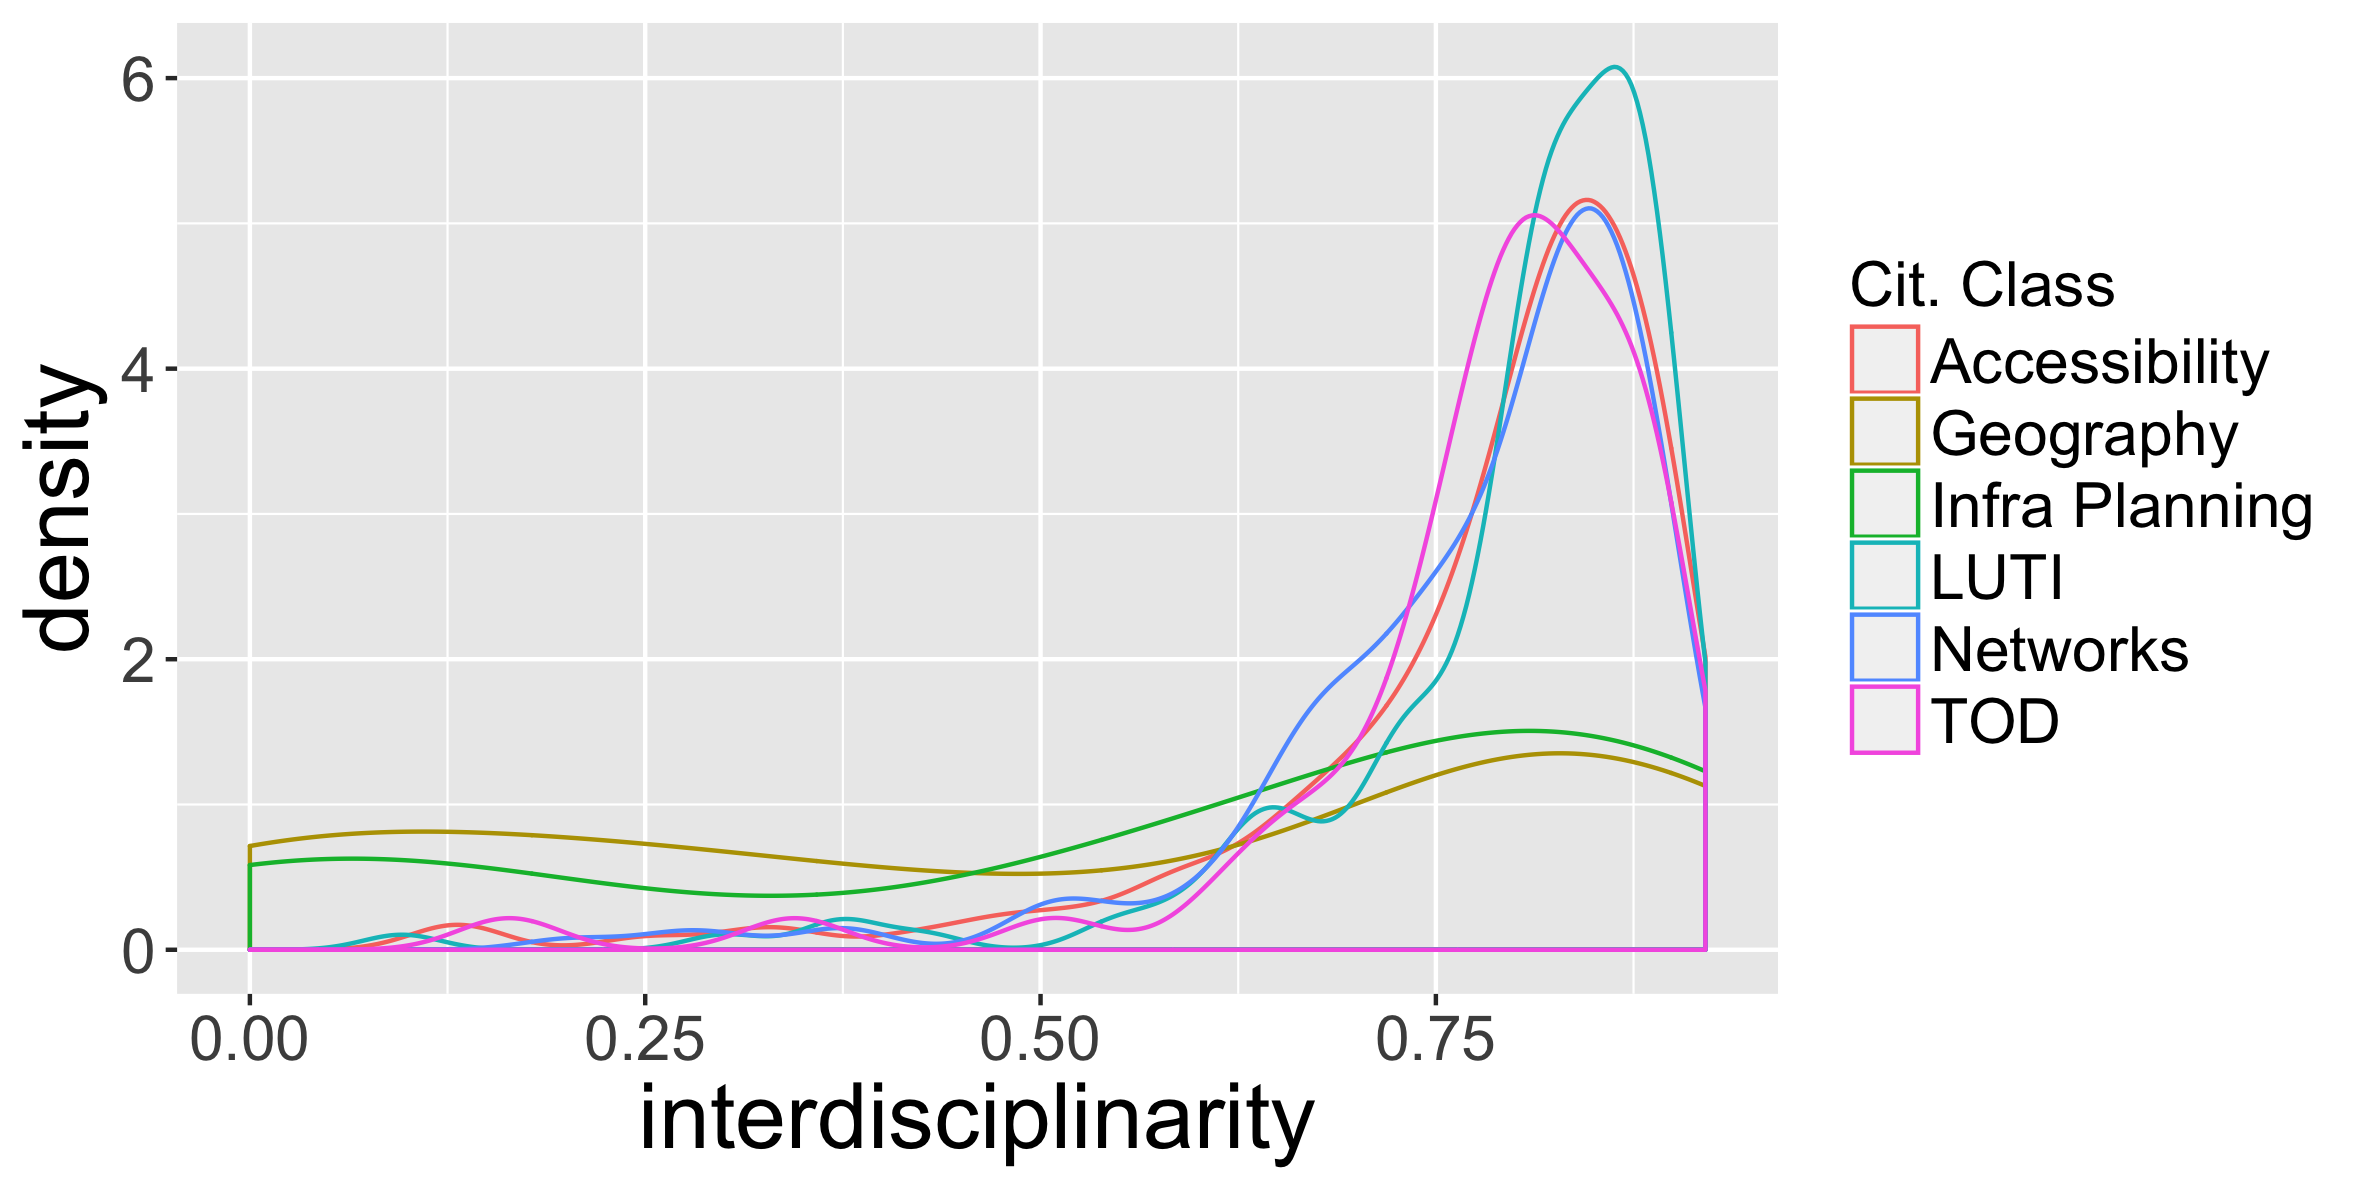
\includegraphics[width=0.49\linewidth]{Figures/QuantEpistemo/interdisciplinarities}
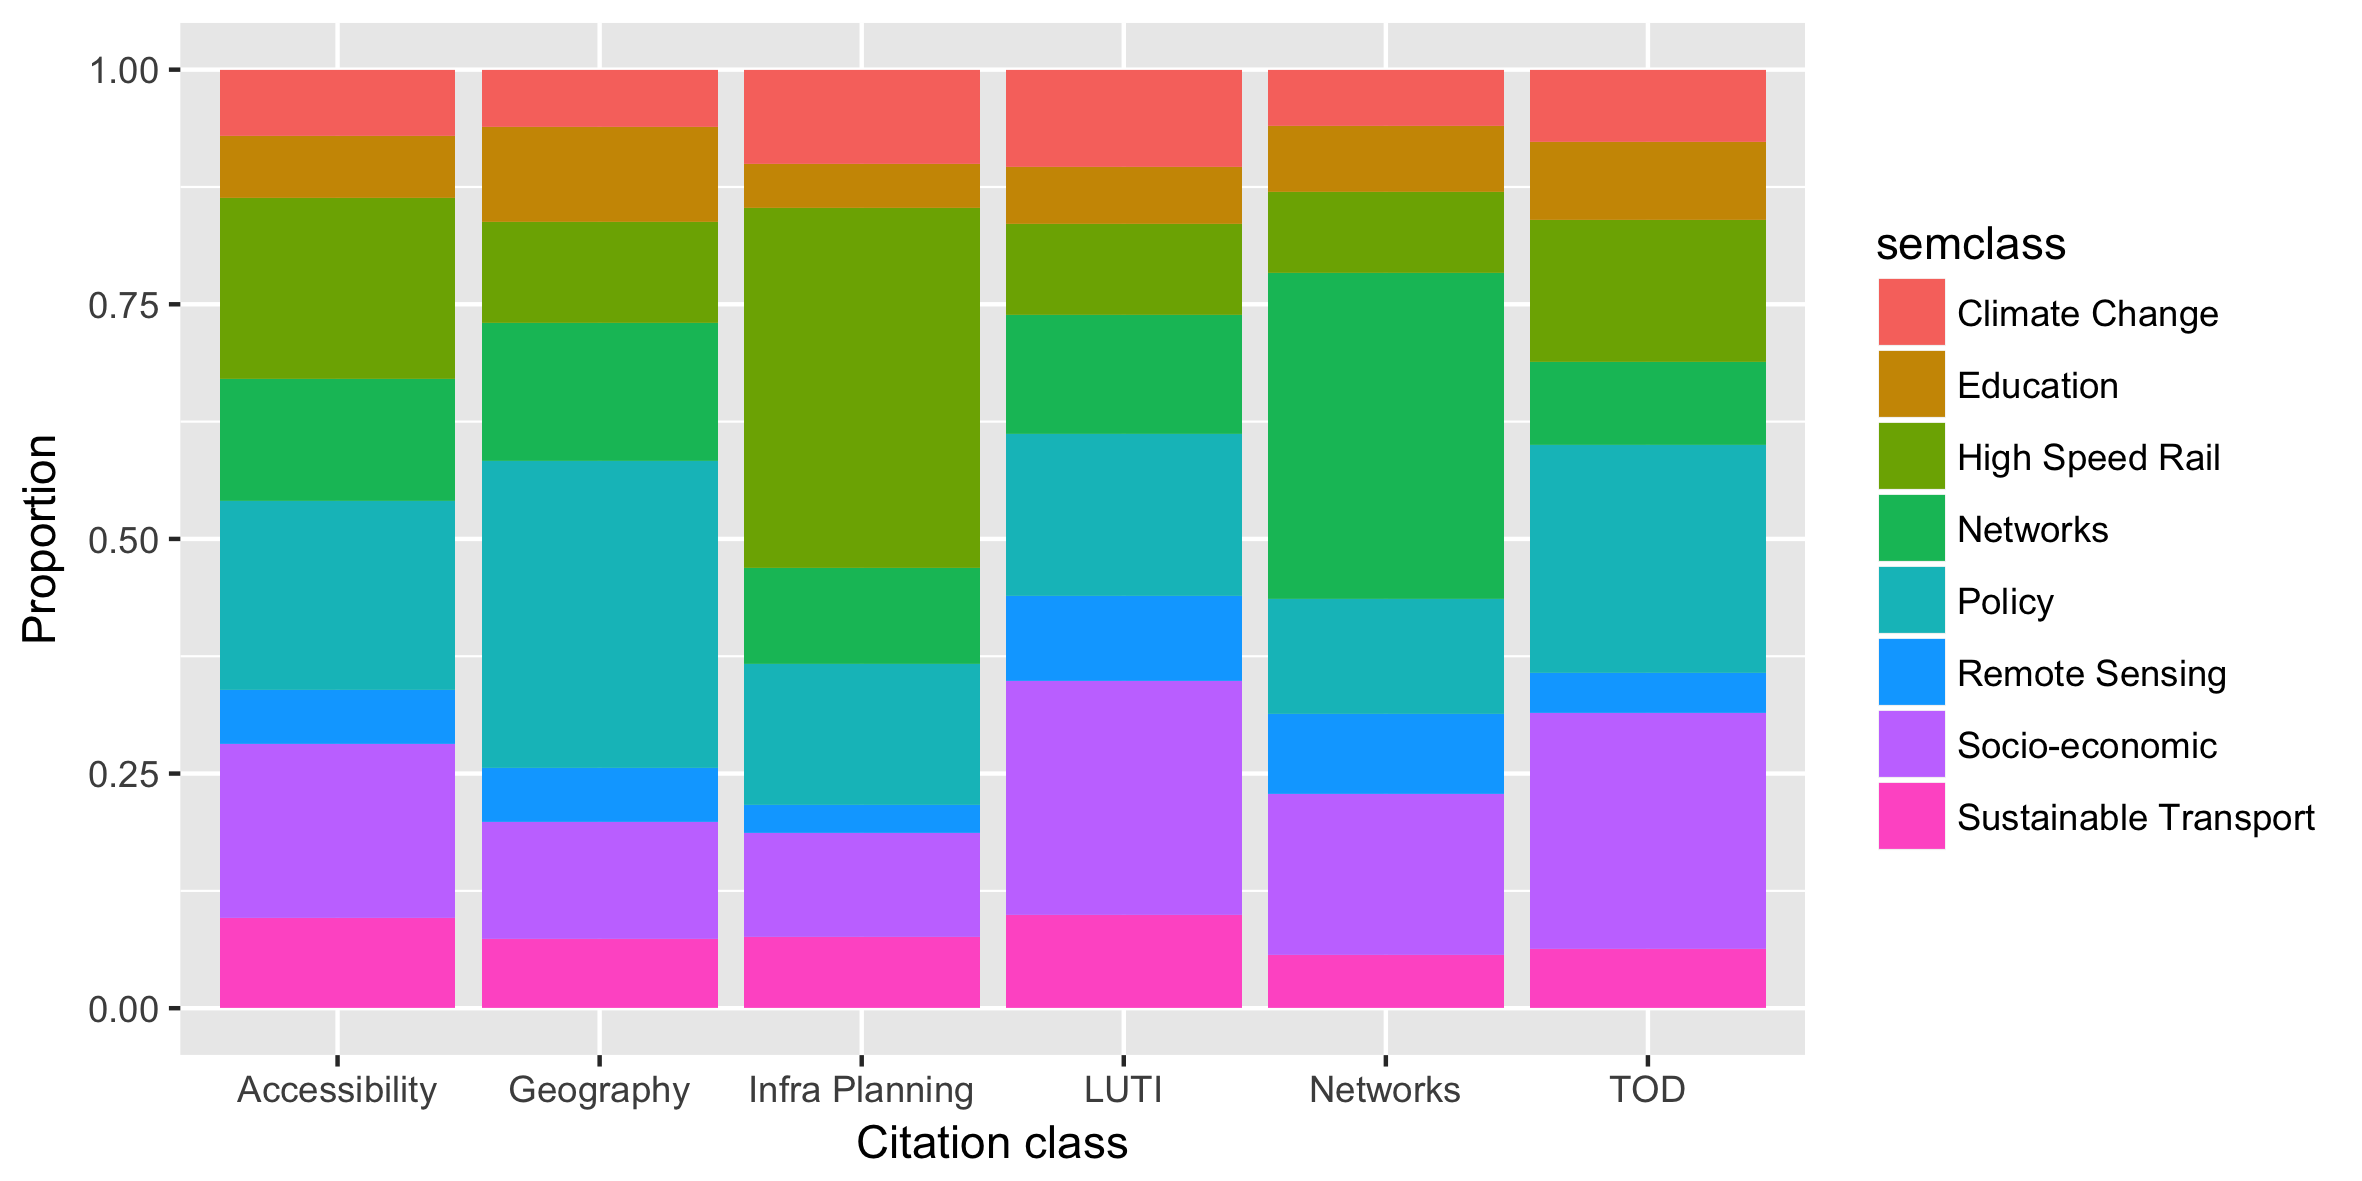
\includegraphics[width=0.49\linewidth]{Figures/QuantEpistemo/compo_proportion}\\
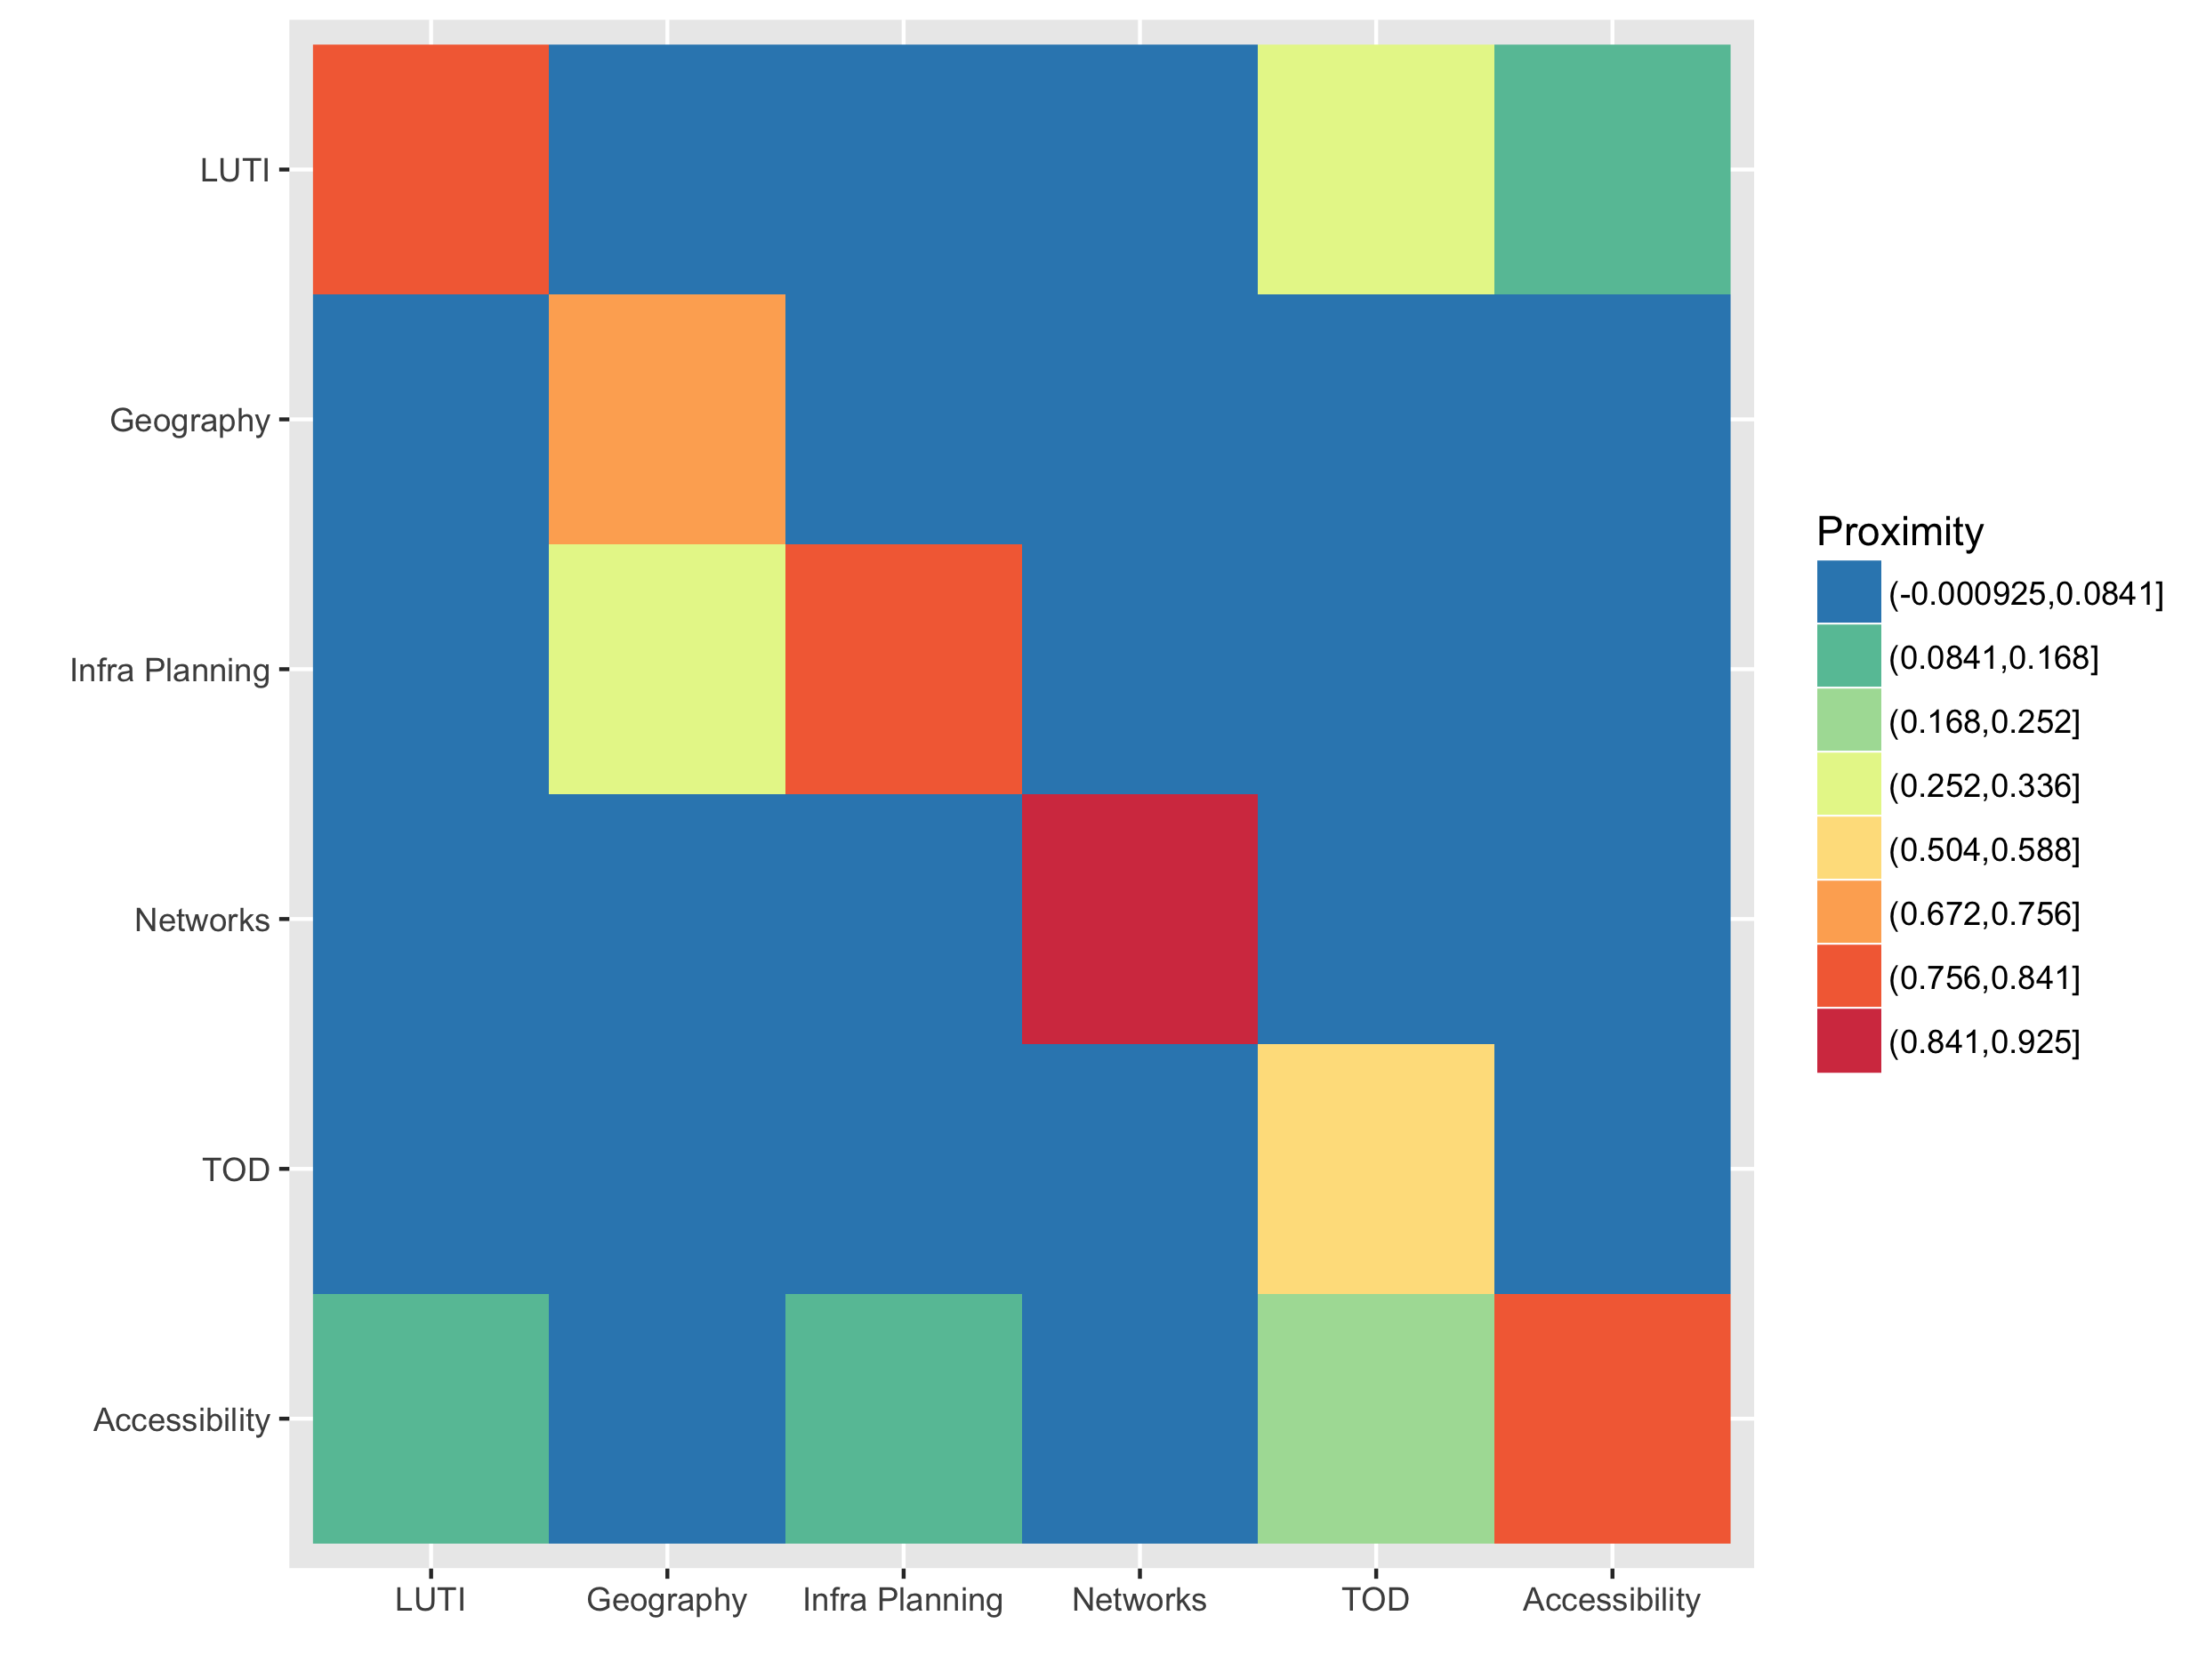
\includegraphics[width=0.49\linewidth]{Figures/QuantEpistemo/citation_proximities}
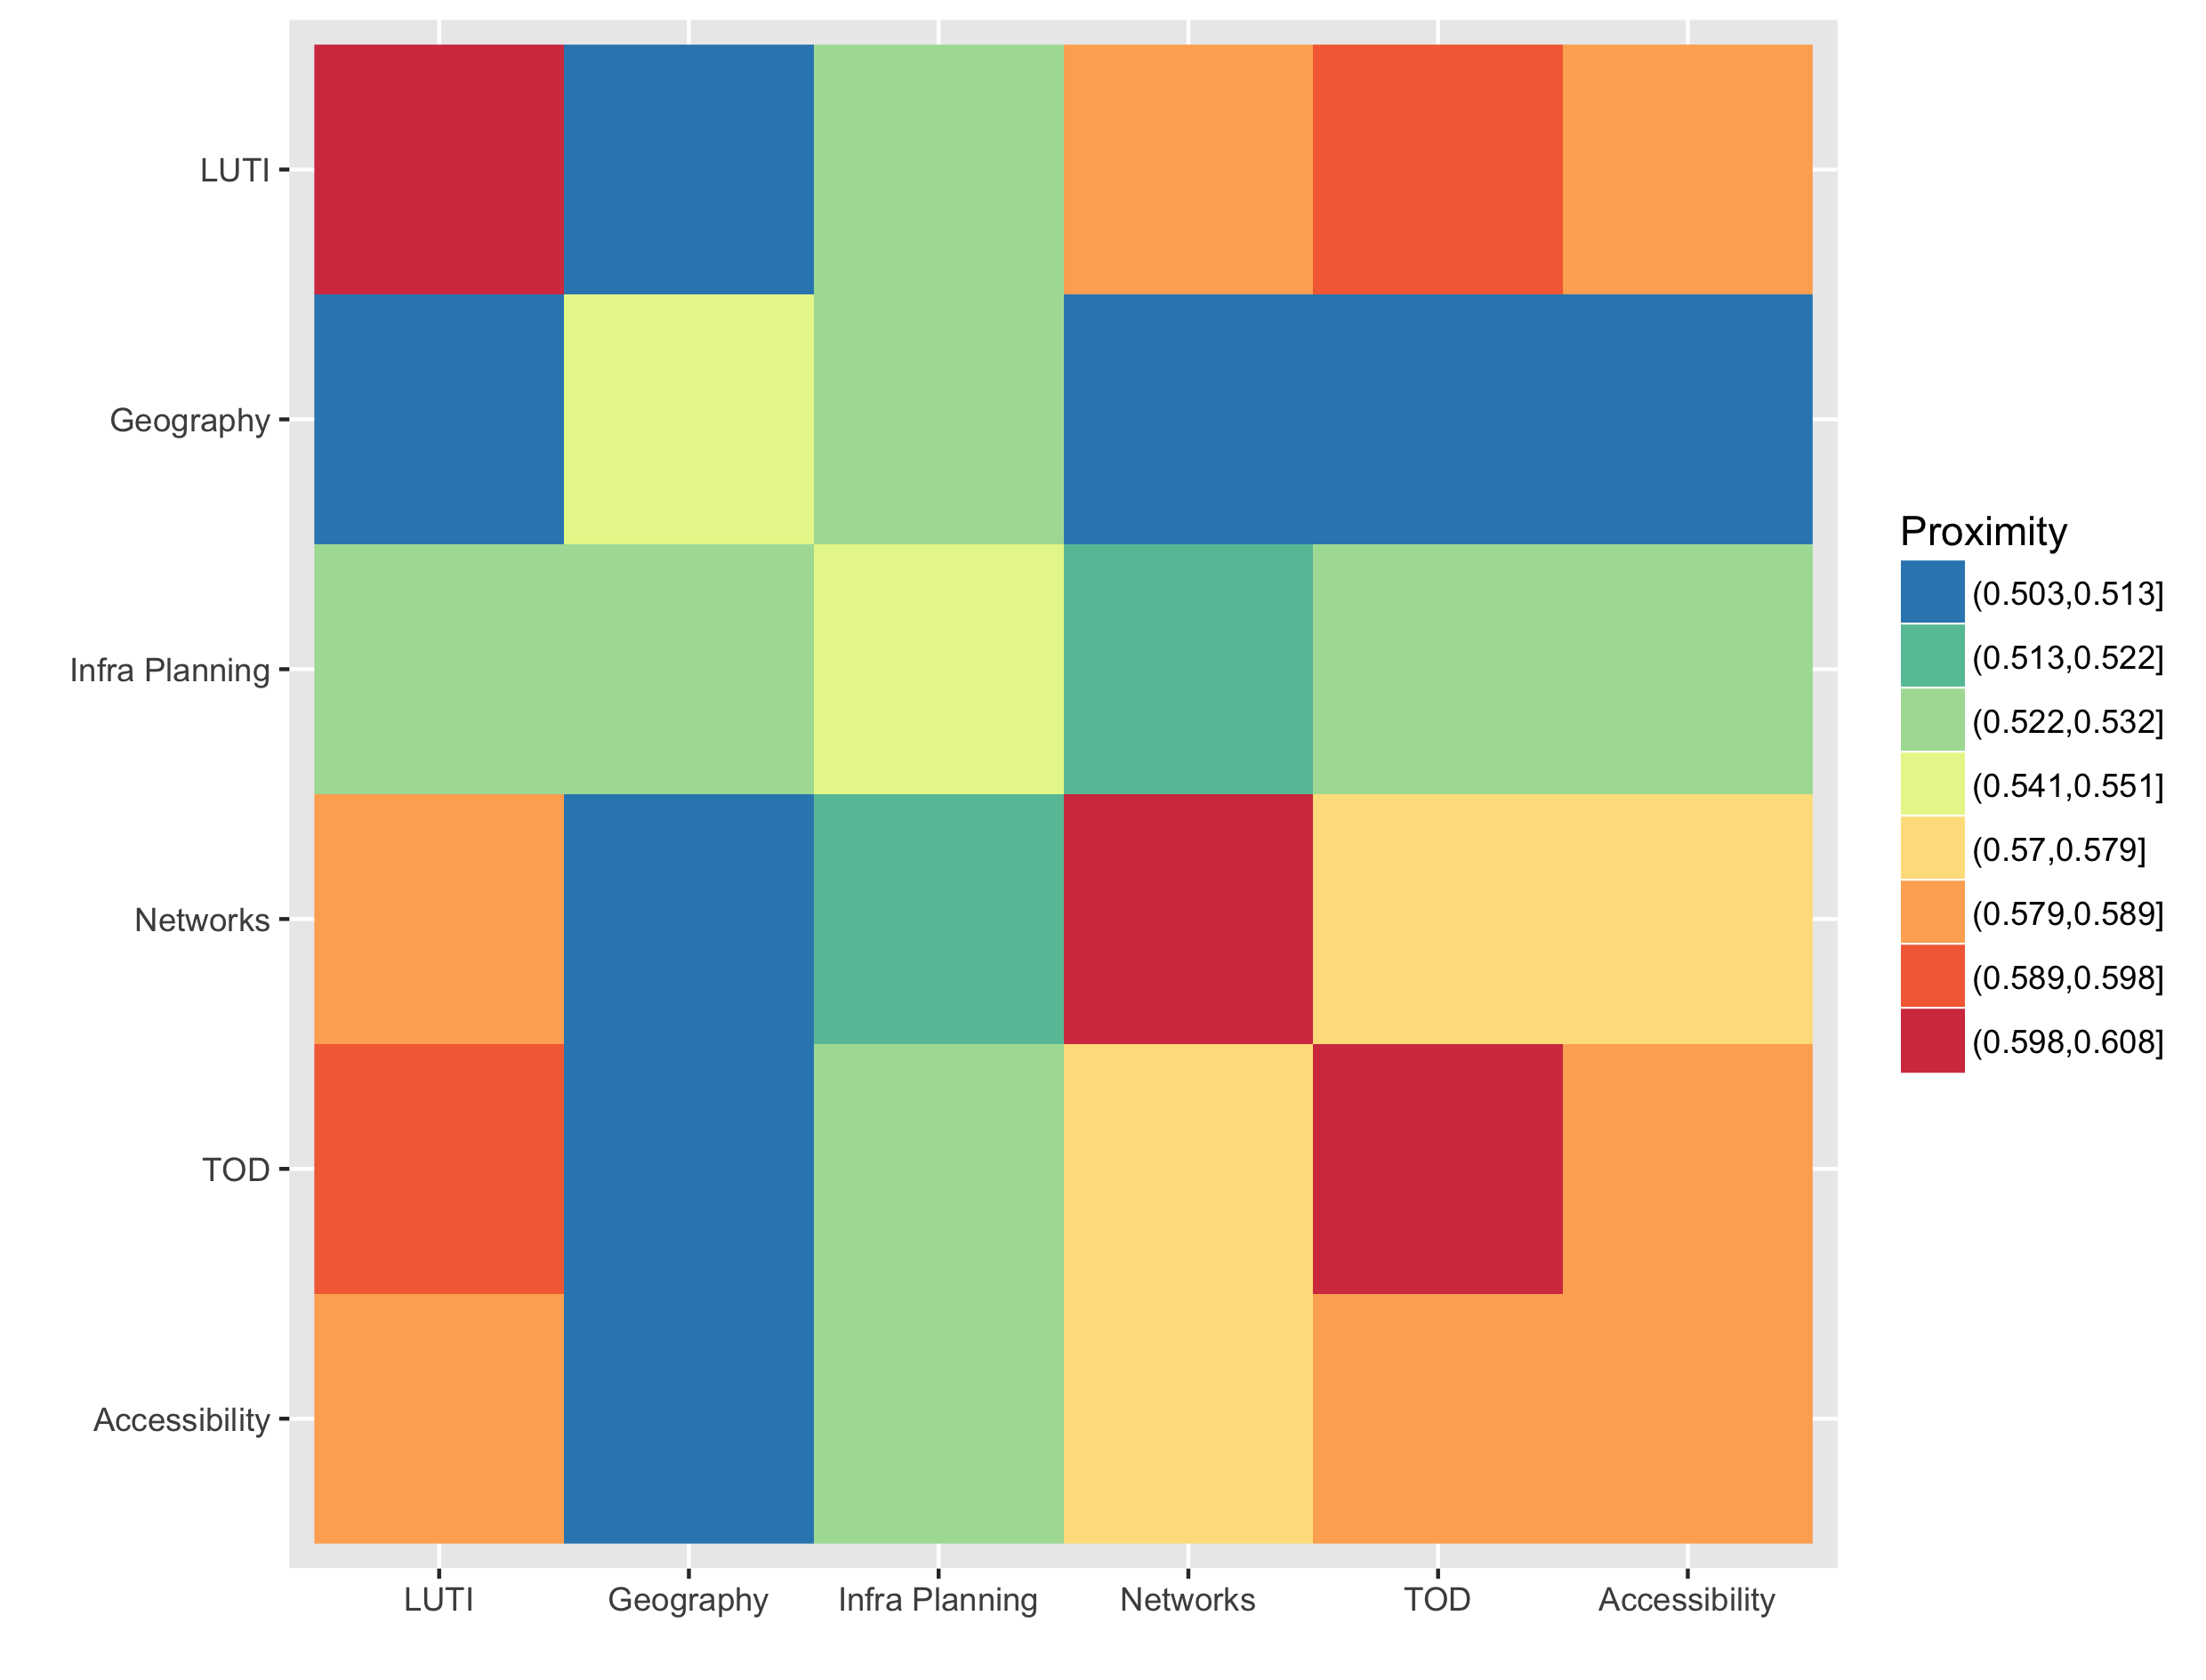
\includegraphics[width=0.49\linewidth]{Figures/QuantEpistemo/semantic_proximities}
\caption[][Motifs d'interdisciplinarité]{\label{fig:quantepistemo:interdisc}}{\textbf{Motifs d'interdisciplinarité.} \textit{(Haut Gauche)} Distribution des $I_i$ par classes de citations ; \textit{(Haut Droite)} Composition sémantiques des classes de citation ; \textit{(Bas Gauche)} Matrice de proximité de citation $c_{kk'}$ entre classes de citations ; \textit{(Bas Droite)} Matrice de proximité sémantique $s_{kk'}$ entre classes de citations.\label{fig:quantepistemo:interdisc}\comment[FL]{tu compares les disciplines entre elles mais pas la facon dont elles attaquent les questions au coeur de ta these. c'est dommage.}[(JR)c'est l'objet de la section suivante]}
\end{figure}
%%%%%%%%%%%%%%%%%%



% bootstrap
%min(corrs);max(corrs);mean(abs(corrs))
% -0.170952  0.5496791  0.08384802
% apply(bcorrs,2,mean)
%       minrho        maxrho    meanabsrho     minrhosup     maxrhosup meanabsrhosup 
%  -0.08792137    0.11690677    0.03137750   -0.17686637    0.68579406    0.11079253 
% apply(bcorrs,2,sd)
%       minrho        maxrho    meanabsrho     minrhosup     maxrhosup meanabsrhosup 
%  0.012683338   0.021324056   0.002250636   0.038402781   0.134996447   0.051553244 

% modularities
% sem : 0.1053156
% cit : 0.8140818
% bootstrap N=100
% sem : 0.073097051446193 +- 0.00307154703966512
% cit : 0.204223565075042 +- 0.0141450119581389


\bpar{
}{
Nous concluons cette analyse par une approche plus robuste pour quantifier les proximités entre couches de l'hyperréseau. Il est aisé de construire une matrice de corrélation entre deux classifications, par les corrélations de leur colonnes. Nous définissons les probabilités $\mathbf{P}_C$ toutes égales à 1 pour la classification de citation. La matrice de correlation de celle-ci avec $\mathbf{P}$ s'étend de -0.17 à 0.54 et a une moyenne de valeur absolue de 0.08, ce qui est significatif par rapport à des classifications aléatoire puisque un bootstrap à $b=100$ répétitions avec les matrices mélangées donne un minimum à $-0.08 \pm 0.012$, un maximum à $0.11 \pm 0.02$ et une moyenne absolue à $0.03 \pm 0.002$. Cela montre que les classifications sont complémentaires et que cette complémentarité est significative statistiquement par rapport à des classifications aléatoires. L'adéquation de la classification sémantique par rapport au réseau de citation peut également être quantifiée par la modularité multi-classes~\cite{nicosia2009extending} (voir~\ref{sec:app:patents} pour une définition mathématique), qui traduit la probabilité qu'un lien soit dû à la classification étudiée, en prenant en compte l'appartenance simultanée à de multiples classes. Ainsi, la modularité multi-classes des probabilités sémantiques pour le réseau de citation est de 0.10, ce qui d'une part est significativement signe d'adéquation, un bootstrap toujours à $b=100$ donnant une valeur de $0.073 \pm 0.003$, qui reste limitée vu la valeur maximale fixée par les probabilités de citations dans leur propre réseau qui donnent une valeur de 0.81, ce qui confirme d'autre part la complémentarité des classifications.
}








%--------------------------------------------------------------



%%%%%%%%%%%%%%%%%%%%%%%%
\subsection{Discussion}{Discussion}




\subsubsection{Towards modeling purpose and context automatic extraction}{Vers une modélisation des thèmes et une extraction automatique du contexte}


\bpar{
A possible direction to strengthen our quantitative epistemological analysis would be to work on full textes related to the modeling of interaction between networks and territories, with the aim to automatically extract thematics within articles. The idea would be to perform some kind of automatized modelography, with possible features to be extracted that would be ontologies, model architecture or structures, scales, or even typical parameter values. It is not clear to what degree structure of models can be extracted from their description in papers and it surely depends on the discipline considered. For example in a framed field such as transportation planning, using a pre-defined ontology (in the sense of dictionary) and a fuzzy grammar could be efficient to extract information as the discipline is relatively formatted. In theoretical and quantitative geography, beyond the barrier of language, information organisation is surely less subject to unsupervised data-mining because of the more literary nature of the discipline : synonyms and figures of speech are generally the norm in good level human sciences writing, fuzzing a possible generic structure of knowledge description. 
}{
Une direction possible pour renforcer cette analyse en épistémologie quantitative serait de travailler sur les textes complets des références contenant des efforts de modélisation des interactions entre réseaux et territoires, avec le but d'extraire automatiquement les thématiques des articles. Des méthodes plus adaptées pour les long texte que celle utilisée ici incluent par exemple l'Allocation Latente de Dirichlet~\cite{blei2003latent}. L'idée serait de procéder à une sorte de modélographie automatique\comment[AB]{référence thèse Clara ?}[oui !], pour extraire des caractéristiques telle les ontologies, l'architecture ou la structure des modèles, les échelles ou même des valeurs typiques des paramètres. Il n'est pas clair dans quelle mesure la structure des modèles peut être extraite de leur description dans un article, et cela dépend sûrement de la discipline considérée. Par exemple dans un champ relativement cadré comme la planification des transports, l'utilisation d'une ontologie pré-définie (dans le sens d'un dictionnaire) et d'une grammaire floue pourrait être efficace vu les conventions assez strictes dans la discipline. En géographie théorique et quantitative, au-delà de la barrière du language\comment[FL]{?}, l'organisation de l'information est sûrement plus délicate à appréhender par de l'apprentissage non-supervisé à cause de la nature plus littéraire de la discipline : les synonymes et les figures de style sont généralement la norme pour l'écriture d'un bon niveau en sciences humaines, rendant plus floue une possible structure générique de la description des connaissances.
}


%Depending on extended results of the two previous sections and on thematic requirements (huge need of knowledge on precise models structure, that may appear when trying to construct more specialized operational models), this project may be conducted with more or less investment.




\subsubsection{Reflexivity}{Réflexivité}


\bpar{
The methodology developed here is particularly interesting since it is reflexive, i.e. it can be used on our work itself. Therefore, an other application will be the reflexivity of our thesis : we attend to proceed to similar analysis on our proper bibliography (and possibly its evolution, available via \texttt{git} history), to understand our patterns of knowledge, possible gaps or unveil unexpected developments. The detailed development is done in Appendix~\ref{app:reflexivity}.
}{
La méthodologie que nous avons développé ici est efficace pour offrir des potentialités de réflexivité, c'est à dire qu'elle peut être utilisée pour étudier notre approche elle-même. Une de ses applications, hors de celle à la revue scientifique Cybergeo dans la perspective de Science Ouverte (voir Appendice~\ref{app:sec:cybergeo}), sera à notre propre corpus de références, dans le but de révéler des possibles  directions de recherche ou problématiques exotiques. Il est éventuellement possible de le faire de manière dynamique, grâce à l'historique de \texttt{git} qui permet de récupérer n'importe quelle version de la bibliographie à une date donnée sur les trois ans écoulés. Il s'agira aussi de comprendre nos motifs de production de connaissance afin de contribuer à~\ref{sec:knowledgeframework}. Le développement détaillé est fait en Appendice~\ref{app:reflexivity}.
}





\stars




%
% 2.3 - Modelography



%-------------------------------

\newpage

\section{Systematic Review and Modelography}{Revue Systématique et Modélographie}

\label{sec:modelography}

%-------------------------------


Tandis que les études menées précédemment proposaient de construire un horizon global de l'organisation des disciplines s'intéressant à notre question, nous proposons à présent une étude plus ciblée des caractéristiques de modèles existants. Nous proposons pour cela dans un premier temps une revue systématique, c'est à dire la construction d'un corpus plus précis répondant à certaines contraintes, suivie d'une meta-analyse, c'est à dire une tentative d'explication de certaines caractéristiques des modèles par des modèles statistiques.


%%%%%%%%%%%%%%%%%%%%
%\subsection[Systematic Review][Revue Systématique]{Systematic Review and Meta-analysis}{Revue systématique et Meta-analyse}
\subsection{Systematic Review and Meta-analysis}{Revue systématique et Meta-analyse}



Les revues systématiques classiques ont majoritairement lieu dans des domaines où une recherche très ciblée, même par titre d'article, fournira un certain nombre d'études étudiant quasiment la même question : typiquement en évaluation thérapeutique, où des études standardisées d'une même molécule varient uniquement par taille des effectifs et modalités statistiques (groupe de contrôle, placebo, niveau d'aveugle). Dans ce cas la construction du corpus est d'une part aisée par l'existence de bases spécialisées permettant des recherches très ciblées, et d'autre part par la possibilité de procéder à des analyses statistiques supplémentaires pour croiser les différentes études (par exemple meta-analyse par réseau, voir~\cite{rucker2012network}). Dans notre cas, l'exercice est bien plus aléatoire pour les raisons exposées dans les deux sections précédentes : les objets sont hybrides, les problématiques diverses, et les disciplines variées. Les différents points soulevés par la suite auront souvent autant de valeur thématique que de valeur méthodologique, suggérant des points cruciaux lors de la réalisation d'une telle revue systématique hybride.


Nous proposons une méthodologie hybride couplant les deux méthodologies développées précédemment avec une procédure plus classique de revue systématique. Nous souhaitons à la fois une représentativité de l'ensemble des disciplines que l'on a découvertes, mais aussi un bruit limité dans les références prises en compte pour la modélographie. Nous adoptons pour cela le protocole suivant :

% - 0.95% of edges with higher weight, with nodes in 80% quantile degree of their respective sem class.
% - take pairs (edges) and singles : 2582 kws
% - filter by hand : typically removed : Emissions, Education-cgnitive sci, teledetection, migration, social nws, lieux-pays, tourism-culture, social inequalities etc,  ; and too general : spillover e.g.  -> 115kws
% - request : can ask for 20 in that case
% - corpus : 2001 references
% - manual screening (title) 
%    * we already remove mobility studies (other scale) to limit final corpus
%    * pedestrian models
%    * traffic
%    * random stuffs
%    * design only (transport or lu independently) (≠ nw growth Tero)
%    * travel behavior : impact car ownersjip urb form, impact biofuel policies US, 
%    * ecology (habitat)
%    * technical transport
%    * pure eco (agllo eco) Anas urban spatial structure
%    * freight
%
%  -> N = 134 at this stage -> extend with corcit / hand
%  
% - manual screening citcore (N = 1843)
%    * rq : biaisé par titres pas explicites selon domaines (ex Courtat)
%  -> N' = 170
%
% - consolidation : N'' = 297
% 
% - full texts : 
%    * use of sci-hub necessary
%    * what do we mean by model ? (! contradiction with epistemo fwk ? clarifier) modèle de simulation / numérique.
%    * publishers ! : plus de springer, alors que que elsevier et tandf dans premiere section (corpus kws) -> biais request (et tous sur reasearch gate, like shady lit.)
%
% - final corpus : with Model = 145


\begin{enumerate}
\item Partant du corpus de citation isolé en~\ref{subsec:indirectbibliometrics}, nous isolons un nombre de mots-clés pertinents, en sélectionnant les 5\% de liens ayant le plus fort poids (seuil arbitraire), puis parmi les noeuds correspondants ceux ayant un degré supérieur au quantile à 0.8 de leur classe sémantique respective. Le premier filtrage permet de se concentrer sur le ``coeur'' des disciplines observées, et le second de ne pas biaiser par la taille sans perdre la structure globale, les classes étant relativement équilibrées. Un examen manuel permet de supprimer les mots-clés clairement non-pertinents (télédétection, tourisme, réseaux sociaux, \ldots), ce qui conduit à un corpus de $K=115$ mots-clés ($K$ est endogène ici).
\item Pour chaque mots-clé, nous effectuons automatiquement une requête au catalogue (scholar) en y ajoutant \texttt{model*}, d'un nombre fixé $n=20$ de références. L'ajout du terme est nécessaire pour obtenir des références pertinentes, après test sur des échantillons.
\item Le corpus potentiel composé des références obtenues, ainsi que des références composant le réseaux de citation, est revu manuellement (passage en revue des titres) pour assurer une pertinence au regard de l'état de l'art de~\ref{sec:modelingsa}, fournissant le corpus préliminaire de taille $N_p = 297$.
\item Ce corpus est alors inspecté pour les résumés et textes complets si nécessaire. On sélectionne les articles mettant en place une démarche de modélisation, hors modèles conceptuels. Les références sont classifiées et caractérisées selon des critères décrits ci-dessous. On obtient alors un corpus final de taille $N_f = 145$, sur lequel des analyses quantitatives sont possibles.
\end{enumerate}

La méthode est résumée en Fig.~\ref{fig:modelography:systematicreview}, avec les valeurs des paramètres et la taille des corpus successifs. Cet exercice permet tout d'abord un certain nombre de points méthodologiques, dont la connaissance pourra être un atout pour mener des revues systématiques hybrides similaires :

\begin{itemize}
\item Les biais de catalogue semblent inévitables. Nous reposons sur l'hypothèse que l'utilisation de Scholar permet un échantillonnage uniforme au regard des erreurs ou biais de catalogage. Le développement futur d'outils ouverts de catalogage et de cartographie, permettant un effort contributif pour une connaissance plus précise de domaines étendus et de leurs interfaces, sera un enjeu crucial de la fiabilité de ce genre de méthodes (voir~\ref{app:sec:cybergeo}).
\item La disponibilité des textes complets est particulièrement un problème pour une revue si large, vu la multiplicité des éditeurs. L'existence de moyens d'émancipation de la science ouverte comme Sci-hub permet d'effectivement accéder à l'ensemble des textes. En écho au débat sur le bras de fer récent avec les éditeurs concernant l'exclusivité de la fouille de textes complets, il parait de plus en plus évident qu'une science ouverte réflexive est totalement antagoniste au modèle actuel de l'édition. Nous espérons également une évolution rapide des pratiques sur ce point.
\item Les revues, et en fait les éditeurs, semblent influencer différemment les référencements, augmentant potentiellement le biais de requête. La littérature grise ainsi que les pre-prints sont pris en compte différemment selon les champs.
\item Le passage en revue manuel des grand corpus permet de pas louper des ``poids lourds'' qui auraient pu être omis en amont~\cite{lissacksubliminal}. La question de la mesure dans laquelle on peut s'attendre d'être au courant de la manière la plus exhaustive des découvertes récentes liées au sujet étudié évolue très probablement vu l'augmentation de la quantité totale de littérature produite et la fragmentation des domaines pour certains toujours plus pointus~\cite{bastian2010seventy}. Rejoignant les points précédents, on peut supposer que des outils d'aide à l'analyse systématique permettront de garder cet objectif raisonnable.
\item Les résultats de la revue automatique sont sensiblement différents des domaines dessinés dans la revue classique : certaines associations conceptuelles, notamment l'inclusion des modèles de croissance de réseaux, ne sont pas naturelles et existent peu dans le paysage scientifique comme nous l'avons montré précédemment.
\end{itemize}


D'autre part, l'opération de construction du corpus permet déjà en elle-même de tirer des observations thématiques intéressantes en elles-mêmes :

\begin{itemize}
\item Les articles sélectionnés supposent une clarification de ce qui est entendu par ``modèle''. Nous donnons en~\ref{sec:knowledgeframework} une définition très large s'appliquant à l'ensemble des perspectives scientifiques. Notre selection ici ne retient pas les modèles conceptuels par exemple, notre critère de choix étant que le modèle doit inclure un aspect numérique ou de simulation.
\item Un certain nombre de références consistent en des revues, ce qui revient à un groupe de modèles ayant des caractéristiques similaires. On pourrait compliquer la méthode en retranscrivant chaque revue ou meta-analyse, ou en pondérant par le nombre d'article correspondant les enregistrements des caractéristiques correspondants. Nous faisons le choix d'ignorer ces revues, ce qui reste cohérent de manière thématique en restant dans l'hypothèse d'échantillonnage uniforme.
\item Une première clarification du cadre thématique est opérée, puisque nous ne sélectionnons pas les études liées uniquement au traffic et à la mobilité (ce choix étant aussi lié aux résultats obtenus en~\ref{sec:transportationequilibrium}), à l'urban design pur, au modèles de flux piétons, au fret, à l'écologie, aux aspects techniques du transport, pour donner quelques exemples, même si ces sujets peuvent dans une vue extrême être considérés comme liés aux interactions entre réseaux et territoires.
\item De la même façon, des domaines annexes comme le tourisme, les aspects sociaux de l'accès aux transports, l'anthropologie, n'ont pas été pris en compte.
\item On observe une forte fréquence des études liées au Trains à Grande Vitesse (HSR), rappelant la non-dissociabilité des aspects politiques de la planification et des directions de recherche en transports.%, surtout en France où les Corpsards des Ponts ou des Mines ont une main mise relative sur les deux aspects simultanément.
\end{itemize}


%%%%%%%%%%%%%%%
\begin{figure}[h!]
\frame{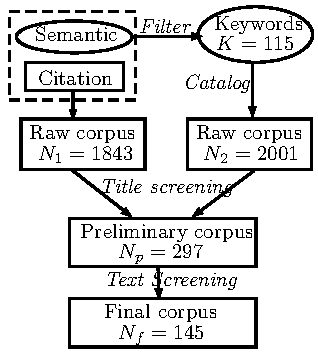
\includegraphics[width=\textwidth]{Figures/Modelography/systematicreview}}
\caption[Systematic Review][Revue Systématique]{\label{fig:modelography:systematicreview}}{\textbf{Méthodologie de la revue systématique.} Les rectangles désignent des corpus de références, les ellipses des corpus de mot-clés, et les pointillés les corpus initiaux. A chaque étape est donnée la taille du corpus.\label{fig:modelography:systematicreview}}
\end{figure}
%%%%%%%%%%%%%%%




%%%%%%%%%%%%%%%%%%%%
\subsection{Modelography}{Modélographie}


Nous passons à présent à une analyse mixte basée sur ce corpus, inspirée par les résultats des sections précédentes précédents notamment pour la classification. Elle a pour but d'extraire et de décomposer précisément les ontologies, échelles et processus, puis d'étudier des liens possibles entre ces caractéristiques des modèles et le contexte dans lequel ils ont été introduits. Il s'agit ainsi de la meta-analyse en quelque sorte, que nous désignerons ici par modélographie. Pour ne pas froisser les puristes, il ne s'agit en effet pas d'une meta-analyse à proprement parler car nous ne combinons pas des analyses proches pour extrapoler des résultats potentiels d'échantillons plus grand. Notre démarche est proche de celle de \noun{Cottineau} dans~\cite{2016arXiv160606162C} qui rassemble les références ayant étudié quantitativement la loi de Zipf pour les villes, puis lie les caractéristiques des études aux méthodes utilisées et hypothèses formulées.


La première partie consiste en l'extraction des caractéristiques des modèles. Automatiser ce travail constituerait un projet de recherche en lui-même, comme nous développons en discussion ci-dessous, mais nous sommes convaincus de la pertinence d'affiner de telles techniques (voir~\ref{ch:opening}) dans le cadre d'un développement de disciplines intégrées. Le temps étant autant l'ennemi que l'allié de la recherche, nous nous concentrons ici sur une extraction manuelle qui se voudra plus fine qu'une tentative peu convaincante de fouille de données. Nous extrayons des modèles les caractéristiques suivantes :

\begin{itemize}
\item Quelle est la force du couplage entre les ontologies territoriales et celles du réseau, autrement dit s'agit-il d'un modèle de co-évolution. Nous classerons pour cela en catégories suivant la représentation de la figure~\ref{fig:modelography:coevolution} : \texttt{\{territory ; network ; weak ; coevolution\}}, qui résulte de l'analyse de la littérature en~\ref{sec:modelingsa}.
\item Echelle de temps maximale. % et minimale (journalier, annuel, décade(s), siècle(s)) ; Multi-echelles temporelles (booléen)
\item Echelle d'espace maximale. %et minimale (local, ville, régional, système de ville) ; Multi-echelles spatiales (booléen)
\item Hypothèses d'équilibre.
\item Domaine ``a priori'', déterminé par l'origine des auteurs et domaine de la revue.
\item Méthodologie utilisée (modèles statistiques, système d'équations, multi-agent, automate cellulaire, recherche opérationnelle, simulation etc.).
\item Cas d'étude (ville, métropole, région ou pays) s'il y a lieu.
\end{itemize}

Nous collectons également de manière indicative, mais sans objectif d'objectivité ni d'exhaustivité, le ``sujet'' de l'étude (c'est à dire la question thématique dominante) ainsi que les ``processus'' inclus dans le modèle. Une extraction exacte des processus reste hypothétique, d'une part conditionnée à une définition rigoureuse et prenant en compte différents niveaux d'abstraction, de complexité, ou d'échelle, d'autre part dépendant de moyens techniques hors de portée de cette étude modeste. Nous commenterons ceux-ci de manière indicative sans les inclure dans les études systématiques.


%%%%%%%%%%%%%%%%%
\begin{figure}[h!]
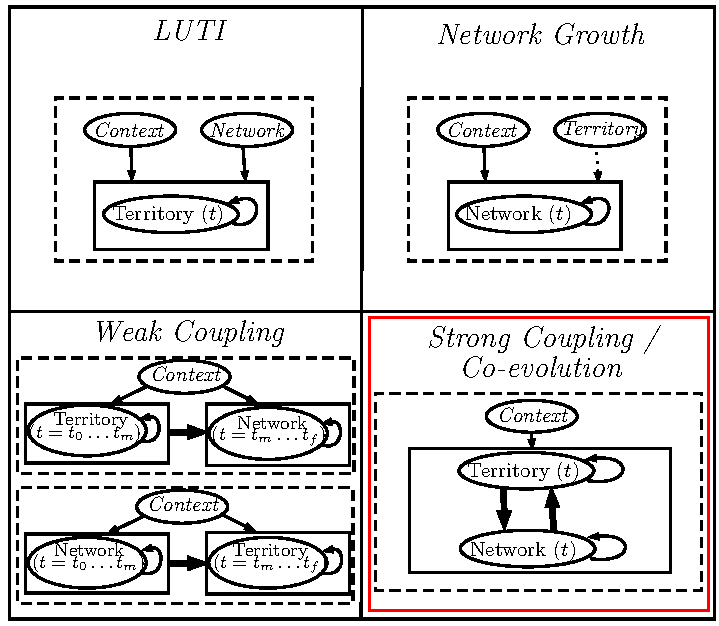
\includegraphics[width=\linewidth]{Figures/Modelography/coevolution}
\caption[Coupling types][Types de couplages]{Schematic representation of the distinction between different types of models coupling networks and territories \label{fig:modelography:coevolution}}{\textbf{Représentation schématique de la distinction entre différents types de modèles couplant territoires et réseaux.} Les ontologies sont représentés par des ovales, les sous-modèles par les boîtes pleines, les modèles par les boîtes pointillées, les couplages par les flèches. Nous surlignons en rouge l'approche qui sera l'objectif final de notre travail.\label{fig:modelography:coevolution}}
\end{figure}
%%%%%%%%%%%%%%%%%

Nous confondons également échelle, portée et dans un sens résolution pour ne pas rendre plus confus l'extraction. Même s'il serait pertinent de différencier lorsque un élément n'a pas lieu d'être pour un modèle (NA) de lorsque celui-ci est mal défini par son auteur, cette tâche apparaît sujette à subjectivité et nous fusionnons les deux modalités. Nous ajoutons aux caractéristiques ci-dessus les variables suivantes :

\begin{itemize}
\item Domaine de citation (le cas échéant, c'est à dire pour les références initialement présentes dans le réseau de citation, i.e. 55\% des références)
\item Domaine sémantique, défini par le domaine pour lequel le document a la plus grande probabilité
\item Indice d'interdisciplinarité
%\item Interdisciplinarité au second ordre (le cas échéant, pour les références consistant en les deux premiers niveaux du réseau de citation)
\end{itemize}

Les domaines sémantiques et la mesure d'interdisciplinarité ont été recalculés pour ce corpus par collecte des mots-clés, puis extraction selon la méthode décrite en~\ref{sec:quantepistemo}, avec $K_W=1000$, $\theta_w=15$ et $k_{max}=500$. On obtient des communautés plus ciblées et plutôt représentatives de la thématique et des méthodes : Transit-oriented development (\texttt{tod}), Hedonic models (\texttt{hedonic}), Planification des infrastructures (\texttt{infra planning}), High-speed rail (\texttt{hsr}) , Réseaux (\texttt{networks}), Réseaux complexes (\texttt{complex networks}), Bus rapid transit (\texttt{brt}).


Un ``bon choix'' de caractéristiques pour classer les modèles est un peu le problème du choix des \emph{features} en apprentissage statistique : si on est en supervisé, c'est à dire qu'on veut obtenir une bonne prédiction de classe fixée a priori (ou une bonne modularité de la classification obtenue par rapport à la classification fixée), on pourra sélectionner les caractéristiques optimisant cette prédiction. On discriminera ainsi les modèles que l'on connait et que l'on juge différents. Si l'on veut extraire une structure endogène sans a priori (classification non supervisée), la question est différente. Nous testerons pour cela en second temps une technique de regression qui permet d'éviter l'overfitting et faire de la selection de caractéristiques (forêts aléatoires).



\paragraph{Processes and Case studies}{Processus et cas d'étude}

Concernant l'existence d'un cas d'étude et sa localisation, 26\% des études n'en présentent pas, correspondant à un modèle abstrait ou modèle jouet (la quasi totalité des études en physique tombant dans ce cas). Ensuite, elles sont réparties à travers le monde, avec toutefois une surreprésentation des Pays-bas avec 6.9\%. Les processus inclus sont trop variés (en fait autant que les ontologies des disciplines concernées) pour faire l'objet d'une typologie, mais on notera la domination de la notion d'accessibilité (65\% des études), puis des processus très variés allant de processus de marché immobilier pour les études hédoniques, aux relocalisations d'actifs et d'emplois pour les luti, ou aux investissements d'infrastructure de réseau. On observe des processus abstraits géométriques de croissance de réseau, correspondant aux travaux des physiciens. La maintenance du réseau apparait dans une étude, ainsi que l'histoire politique. Les processus abstraits d'agglomération et dispersion sont aussi le coeur de quelques études. Les interactions entre villes sont minoritaire, les approches de type système de villes étant noyées dans les études d'accessibilité. Les questions de gouvernance et de régulation ressortent aussi, plutôt dans le cas de planification d'infrastructure et de modèle d'évaluation de démarches TOD, mais sont aussi minoritaires. On retiendra que chaque domaine puis chaque étude introduit ses propres processus quasi-spécifiques à chaque cas.



\paragraph{Corpus Characteristics}{Caractéristiques du corpus}

% DISCIPLINE
% biology computer science        economics      engineering      environment 
%       0.6896552        0.6896552       30.3448276        2.0689655        0.6896552 
%       geography          physics         planning   transportation 
%      19.3103448        8.2758621       20.0000000       17.9310345 
%
% SEMANTIC
%             brt complex networks          hedonic              hsr   infra planning 
%       0.6896552        0.6896552       11.0344828        2.7586207        5.5172414 
%        networks              tod 
%      20.6896552       27.5862069 

Les domaines ``a priori'' (i.e. jugés, ou plutôt préjugés sur la revue ou l'appartenance des auteurs), sont relativement équilibrés pour les disciplines majoritaires déjà identifiées\comment[FL]{B} : 17.9\% Transportation, 20.0\% Planning, 30.3\% Economics, 19.3\% Geography, 8.3\% physics, le reste minoritaire se répartissant entre environnement, informatique, ingénierie et biologie. Concernant les poids des domaines sémantiques significatifs, le TOD domine avec 27.6\% des documents, suivi par les réseaux (20.7\%), les modèles hédoniques (11.0\%), la planification des infrastructures (5.5\%) et le HSR (2.8\%). Les contingences montrent que le Planning ne fait quasiment que du TOD, la physique uniquement des réseaux, la géographie se répartit équitablement entre réseaux et TOD (le second correspondant aux articles typés ``aménagement'', qui ont été classés en géographie car dans des revues de géographie) ainsi qu'une plus faible part en HSR, enfin l'économie est la plus variée entre hédonique, planning, réseaux et TOD. Cette interdisciplinarité n'apparait cependant que pour les classes extraites pour la probabilité majoritaire, puisque les indices d'interdisciplinarité moyens par discipline ont des valeurs équivalentes (de 0.62 à 0.65), hormis la physique significativement plus basse à 0.56 ce qui confirme son statut de ``nouveau venu'' ayant une profondeur thématique plus faible.


Il est intéressant pour notre question de répondre à la question ``qui fait quoi ?'', c'est à dire quelles types de modèles sont mobilisés par les différentes disciplines. Nous donnons en Table~\ref{tab:modelography:what} la table de contingence du type de modèle en fonction des disciplines a priori, de la classe de citation et de la classe sémantique. On constate les approches fortement couplées, les plus proches de ce qu'on considère comme des modèles de co-évolution, sont majoritairement contenues dans le vocabulaire des réseaux, ce qui est confirmé par leur positionnement en terme de citation, mais que les disciplines concernées sont variées. La majorité des études s'intéresse au territoire uniquement, le déséquilibre le plus fort étant pour les études sémantiquement liées au TOD et à l'hédonique. La physique est encore limitée en s'intéressant exclusivement aux réseaux. 


%%%%%%%%%%%%%
\begin{table}
\caption[Model type][Type de modèles]{Model type}{\textbf{Type de modèles étudiés selon les différentes classifications.} Tables de contingence de la variable discrete donnant le type de modèle (réseau, territoire ou couplage fort), pour la classification a priori, la classification sémantique et la classification de citation.}
\label{tab:modelography:what}
\begin{tabular}{|m{2cm}|m{2cm}m{2cm}m{2cm}m{2cm}m{2cm}|}
\hline
Discipline  &  economics & geography & physics & planning & transportation\\\hline
network     &     5      &      3    &   12    &    1     &         4  \\
strong      &     4      &     3     &   0     &   0      &        2  \\
territory   &    35      &    22     &   0     &    28    &         20 \\\hline  
\end{tabular} 
\medskip
\begin{tabular}{|m{2cm}|m{2cm}m{2cm}m{2cm}m{2cm}m{2cm}|}
\hline
Semantic  &  hedonic & hsr & infra planning & networks & tod\\\hline
network   &       1  & 0   &          0     &  14      & 2 \\
strong    &       0  &  0  &            0   &     5    & 1  \\
territory &      15  &  4  &            8   &    11    &  37 \\ \hline
\end{tabular}
\begin{tabular}{|m{2cm}|m{2cm}m{2cm}m{2cm}m{2cm}m{2cm}m{2cm}|}
\hline
Citation  &  Accessibility & Geography & Infra Planning & LUTI & Networks & TOD \\\hline
network   &            0   &     0     &         0      &   0  &     24   &  0 \\
strong    &            0   &      0    &          0     &   2  &      5   &  0 \\
territory &           13   &      1    &          6     &  18  &      2   &  3 \\\hline
\end{tabular}
\end{table}
%%%%%%%%%%%%%



Pour répondre ensuite à la question du comment, on peut regarder les échelles de temps et d'espace typiques des modèles. La planification et les transports se concentrent à des petites échelles spatiales, métropolitain ou local, l'économie également avec une forte représentation du local via les études hédoniques, et une étendue un peu plus grande avec l'existence d'études au niveau régional et quelques une du pays (études de panel généralement). Encore une fois, la physique se retrouve limitée avec l'ensemble de ses contributions à une échelle fixe, métropolitaine (pas forcément claire ni bien spécifiée dans les articles d'ailleurs puisqu'il s'agit de modèles jouets dont les contours thématiques peuvent être très flous). La géographie est relativement bien équilibrée, de l'échelle métropolitaine à l'échelle continentale. Le schéma pour les échelles de temps est globalement similaire. Les méthodes utilisées sont fortement corrélées à la discipline : un test du $\chi^2$ donne une statistique de 169, très significatif avec $p=0.04$. De même, l'échelle d'espace l'est mais de manière moindre ($\chi^2 = 50, p = 0.08$).


\paragraph{Classical Regressions}{Régressions classiques}

Nous étudions à présent l'influence de divers facteurs sur les caractéristiques des modèles par des régressions linéaires simples. Le nombre d'observations pour lesquelles toutes les variables sont renseignées est très faible 

Dans une démarche de multi-modélisation, nous testons l'ensemble des modèles possible pour expliquer la variable à partir des autres, et sélectionnons le meilleur en terme de Critère d'Information d'Akaike.\comment[AB]{expliquer rapidement et référencer en note de bas de page. ; Version simplifiée du tableau de résultats à placer ici ?} 

Les résultats complets des régressions sont donnés en Appendice~\ref{app:sec:modelography}. Les échelles temporelle et d'espace sont les mieux expliquées par les modèles prenant en compte l'ensemble des autres variables. Pour l'échelle de temps, les variables les plus significative sont le fait d'utiliser des méthodes de simulation et le fait d'être en physique, qui tous deux influent négativement. L'échelle spatiale et le fait d'être en planification influent positivement. Au contraire pour l'échelle d'espace, le fait d'être en planning influence négativement alors que le domaine sémantique du TOD est positif, ce qui veut dire que les journaux de planning privilégient des études localisées alors que des problématiques proches ont tendance à étendre l'aire d'étude. Le niveau d'interdisciplinarité est le mieux expliqué par une unique variable, l'année, qui l'influence de manière négative, ce qui confirme l'augmentation des spécialisations scientifiques dans le temps. 




%%%%%%%%%%%%%%%%%
\begin{table}[!htbp]
\caption[][]{\textbf{Explanation of models characteristics.}}{\textbf{Explication des caractéristiques des modèles.}}
\begin{tabular}{lcccccc} 
\footnotesize
\\[-1.8ex]\hline 
\hline \\[-1.8ex] 
 & \multicolumn{6}{c}{\textit{Variable expliquée:}} \\ 
\cline{2-7} 
 & \multicolumn{2}{c}{TEMPSCALE} & SPATSCALE & \multicolumn{2}{c}{INTERDISC} & YEAR \\ 
 & (1) & (2) & (3) & (4) & (5) & (6)\\ 
\hline \\[-1.8ex] 
 YEAR & 0.674 &  &  & $-$0.004$^{*}$ & $-$0.002$^{*}$ &  \\ 
  TYPEstrong &  & 100.271$^{***}$ &  &  & $-$0.026 &  \\ 
  TYPEterritory & $-$38.933$^{***}$ & $-$14.988 &  &  & 0.044 & 10.898$^{***}$ \\ 
  TEMPSCALE &  &  & $-$5.179 & $-$0.0003 &  & 0.035 \\ 
  FMETHODeq &  &  &  &  &  & $-$6.224 \\ 
  FMETHODmap &  &  &  &  &  & 4.747 \\ 
  FMETHODro &  &  &  &  &  & 6.128 \\ 
  FMETHODsem &  &  &  &  &  & 1.009 \\ 
  FMETHODsim &  &  &  &  &  & 5.153 \\ 
  FMETHODstat &  &  &  &  &  & $-$0.357 \\ 
  DISCIPLINEengineering & $-$52.107$^{*}$ & $-$9.609 & $-$154.461 & 0.144 &  & 13.486 \\ 
  DISCIPLINEenvironment & 17.110 & 17.886 & $-$5.878 & 0.092 &  & $-$3.668 \\ 
  DISCIPLINEgeography & 3.640 & 9.126 & 1,445.457$^{***}$ & 0.036 &  & 1.121 \\ 
  DISCIPLINEphysics & 46.879$^{*}$ & 77.897$^{***}$ & 292.559 & $-$0.103 &  & 3.392 \\ 
  DISCIPLINEplanning & 1.304 & 4.553 & $-$143.554 & $-$0.047 &  & $-$2.850 \\ 
  DISCIPLINEtransportation & $-$14.718 & 8.753 & 568.329 & 0.062 &  & 5.503$^{*}$ \\ 
  INTERDISC & 2.357 &  &  &  &  & $-$12.876 \\ 
  SEMCOMcomplex networks &  &  &  &  & $-$0.217 &  \\ 
  SEMCOMhedonic &  &  &  & $-$0.179 & $-$0.184$^{*}$ & $-$5.769 \\ 
  SEMCOMhsr &  &  &  & $-$0.100 & $-$0.122 & 6.135 \\ 
  SEMCOMinfra planning &  &  &  & $-$0.032 & $-$0.096 & $-$4.123 \\ 
  SEMCOMnetworks &  &  &  & $-$0.038 & $-$0.107 & 4.711 \\ 
  SEMCOMtod &  &  &  & $-$0.105 & $-$0.152 & $-$1.653 \\ 
  Constant & $-$1,305.126 & 22.103$^{*}$ & 235.357 & 8.962$^{**}$ & 5.531$^{**}$ & 2,004.945$^{***}$ \\ 
 \hline \\[-1.8ex] 
Observations & 64 & 94 & 94 & 64 & 98 & 64 \\ 
R$^{2}$ & 0.385 & 0.393 & 0.100 & 0.314 & 0.155 & 0.510 \\ 
R$^{2}$ ajusté & 0.282 & 0.336 & 0.027 & 0.136 & 0.068 & 0.281 \\ 
%Residual Std. Error & 26.984 (df = 54) & 31.747 (df = 85) & 1,995.272 (df = 86) & 0.109 (df = 50) & 0.107 (df = 88) & 6.617 (df = 43) \\ 
%F Statistic & 3.755$^{***}$ (df = 9; 54) & 6.871$^{***}$ (df = 8; 85) & 1.369 (df = 7; 86) & 1.761$^{*}$ (df = 13; 50) & 1.789$^{*}$ (df = 9; 88) & 2.234$^{**}$ (df = 20; 43) \\ 
\hline 
\hline \\[-1.8ex] 
\textit{Note:}  & \multicolumn{6}{l}{$^{*}$p$<$0.1; $^{**}$p$<$0.05; $^{***}$p$<$0.01} \\ 
\end{tabular}
\end{table} 
%%%%%%%%%%%%%%%%%




\paragraph{Random Forest Regressions}{Régressions par Forêts Aléatoires}

Nous concluons cette étude par des régressions et classification par Forêts Aléatoires, qui sont une méthode très flexible permettant de dégager une structure d'un jeu de données~\cite{liaw2002classification}. Pour compléter les analyses précédentes, nous proposons de l'utiliser pour déterminer les importances relatives des variables pour différents aspects. Nous utilisons à chaque fois des forêts de taille 100000, une taille de noeud de 1 et un nombre de variable échantillonnée en $\sqrt{p}$ pour la classification et $p/3$ pour la régression lorsque $p$ est le nombre total de variables. Pour classifier le type de modèle, nous comparons les effets de la discipline, de la classe sémantique et de la classe de citation. Cette dernière est la plus importante avec une mesure relative de 45\%, tandis que la discipline compte pour 31\% et le sémantique pour 23\%. Ainsi, le cloisonnement disciplinaire se retrouve, tandis que le sémantique et donc en partie les ontologies, est le plus ouvert. Cela nous encourage dans notre démarche de sortir de ce cloisonnement. Lorsqu'on applique une regression de forêt sur l'interdisciplinarité, toujours avec ces trois variables, on constate qu'elles expliquent 7.6\% de la variance totale, ce qui est relativement faible, témoignant d'une disparité de sémantique sur l'ensemble du corpus indépendamment des différentes classifications. Dans ce cas, la variable la plus importante est la discipline (39\%) suivie par le sémantique (31\%) et la citation (29\%), ce qui confirme que le journal visé conditionne fortement le comportement de langage employé. Cela nous alerte sur le danger de perte de richesse sémantique lorsqu'on s'adresse à un public particulier. Ainsi, nous avons pu dégager certaines structures et régularités des modèles nous concernant, qui seront riches d'enseignements lors de la construction de nos modèles.



%%%%%%%%%%%%%%%%%%%%
\subsection{Discussion}{Discussion}


\paragraph{Further Developments}{Développements}

\bpar{
Further work may consist in the production of an automatic synthesis of this meta-analysis, from a modular modeling point of view, combined with a refined purpose and scale classification. Modular modeling consists in the integration of heterogeneous processes and implementation of processes in order to extract the set of mechanisms giving the best fit to empirical data~\cite{cottineau2015incremental}. We can thus classify models described here according to their building bricks in terms of processes implemented and thus identify possible coupling potentialities.
}{
Un développement possible pourrait consister en la mise en place d'une approche automatique à cette meta-analyse, du point de vue de la modélisation modulaire, combiné avec une classification du but et de l'échelle. La modélisation modulaire consiste en l'intégration de processus hétérogènes et d'implémentation de ces processus dans le but d'extraire les mécanismes donnant la meilleure proximité à des faits stylisés empiriques ou à des données~\cite{cottineau2015incremental}. L'idée serait de pouvoir extraire automatiquement la structure modulaire des modèles existants, à partir des textes complets comme proposé en~\ref{sec:quantepistemo}, afin de classifier ces briques de manière endogène et identifier des couplages potentiels pour des nouveaux modèles.
}



\paragraph{Lessons for Modeling}{Leçons pour la modélisation}


Nous pouvons résumer les points principaux issus de cette méta-analyse qui joueront sur notre attitude et nos choix de modélisation. Tout d'abord, la présence interdisciplinaire des approches effectuant un couplage fort confirme notre besoin de faire des ponts et de coupler les approches, et confirme également rétrospectivement les conclusions de~\ref{sec:quantepistemo} sur les conséquences du cloisonnement des disciplines en terme de modèles formulés. Ensuite, l'importance du vocabulaire des réseaux dans une grande partie des modèles nous poussera à confirmer cet ancrage. La spécificité des approches TOD et d'accessibilité, assez proches des modèles LUTI, seront secondaires pour nous. La portée restreinte des travaux issus de la physique, confirmée par la majorité des critères étudiés, nous pousse à nous méfier de ces travaux et de l'absence de sens thématique aux modèles. La richesse des échelles temporelles et spatiale couvertes par les modèles géographiques et économiques nous confirme l'importance de varier celles-ci dans nos modèles, idéalement de parvenir à des modèles multi-échelles. Enfin, les importances relatives des variables de classification sur le type de modèle vont également dans le sens de ponts interdisciplinaires pour croiser les ontologies.



\paragraph{Synthesis}{Synthèse}

Nous proposons, pour les modèles identifiés comme incluant la co-évolution, de faire une synthèse des ontologies, des processus, des contextes et des échelles pris en compte.


\comment{tableau de type intro partie III pour résumer le contenu des modèles}

\comment[JR]{here fix scales and process, and why morphogenesis and evolutive urban theory}





\stars




%
% Conclusion


%----------------------------------------------------------------------------------------

\newpage

\section*{Synthesis of modeled processes}{Synthèse des processus modélisés}



Nous proposons de synthétiser les processus pris en compte par les modèles parcourus lors de la modélographie, afin de procéder à un effort similaire à celui concluant l'approche thématique du chapitre~\ref{ch:thematic}. Nous ne pouvons ni avoir une vision exhaustive (comme déjà précisé lors de la description de la méthodologie de la modélographie) ni rendre compte avec grande précision de chaque modèle en détail, puisque quasiment chacun est unique dans son ontologie. L'exercice de synthèse permet ainsi de s'extraire de ces limites et prendre un certain recul, et avoir ainsi un aperçu sur les \emph{processus modélisés}\footnote{En gardant en tête les choix de selection, qui emmènent par exemple à ne pas avoir les processus de mobilité dans cette synthèse.}.



%%%%%%%%%%%%%
\begin{table}%[h!]
%\rotatebox{90}{
\caption[Synthesis of processes included in models][Synthèse des processus modélisés]{\textbf{Synthesis of processes included in models.}\label{tab:modelography:processes}}{\textbf{Synthèse des processus modélisés.} Ceux-ci sont classés par échelle, type de modèle et discipline. \label{tab:modelography:processes}}
\begin{tabular}{|l|p{5cm}|p{5cm}|p{5cm}|}
\hline
 & Réseaux $\rightarrow$ Territoires & Territoires $\rightarrow$ Réseaux & Réseaux $\leftrightarrow$ Territoires\\ \hline
\multirow{2}{*}{Micro} &
\textbf{Economie : } marché immobilier, relocalisation, marché de l'emploi & NA & \textbf{Informatique : } croissance spontanée \\\cline{2-2}
& \textbf{Planification : } régulations, développement & & \\\hline
& \textbf{Economie : } marché immobilier, coût du transport, aménités & \textbf{Physique : } corrélations topologiques, hiérarchie, congestion, optimisation locale, maintenance du réseau & \textbf{Economie : } investissements, relocalisations, offre et demande, planification du réseau\\\cline{2-4}
\multirow{2}{*}{Meso}& \textbf{Géographie : } usage du sol, centralité, étalement urbain, effets de réseau & \textbf{Transports : } investissements, niveau de gouvernance & \textbf{Géographie : } usage du sol, croissance du réseau, diffusion de population \\\cline{2-3}
& \textbf{Planification/transports : } accessibilité, usage du sol, relocalisation, marché immobilier & \textbf{Economie : } croissance du réseau, offre et demande & \\\hline
& \textbf{Géographie : } accessibilité, interaction entre villes, relocalisation, histoire politique  & \textbf{Géographie : } interactions entre villes, investissements & \textbf{Economie : } offre et demande \\ \cline{2-4}
\multirow{2}{*}{Macro} & \textbf{Transports : } accessibilité, marché immobilier & \textbf{Transports : } planification de réseau & \textbf{Transports : } couverture du réseau \\\cline{2-3}
& \textbf{Economie : } croissance économique, marché, usage du sol, agglomération, dispersion, compétition & \textbf{Géographie : } interactions entre villes, rupture de potentiel & \\\hline
\end{tabular}
%}
\end{table}
%%%%%%%%%%%%%

% \makecell{\textbf{Physique : } Corrélations topologiques, hiérarchie, congestion, optimisation locale, maintenance du réseau\\\textbf{Transports : } Investissements, Niveau de gouvernance\\\textbf{Economie : } Croissance du réseau, offre et demande }

% Micro & Motifs de mobilité & Congestion du réseau ; Externalités négatives & Mobilité et structure sociale 
% Meso & Relocalisations ; Effets locaux des infrastructures & Rupture de potentiel & Planification métropolitaine ; TOD
% Macro & Interactions entre villes ; Effet tunnel & Différenciation hiérarchique de l'accessibilité &

%\multirow{3}{*}{Territoires $\rightarrow$}& Economie des Réseaux & Moyenne & Mesoscopique & Explication & Rôle de processus économiques & Economie, Gouvernance\\\cline{2-7}


La table~\ref{tab:modelography:processes} propose cette synthèse à partir des 145 articles issus de la modélographie et pour lesquels une classification de type était possible, c'est-à-dire qu'il existait un modèle rentrant dans la typologie développée en~\ref{sec:modelingsa}. Être complètement exhaustif relèverait d'une opération de méta-modélisation interdisciplinaire qui est bien hors de la portée de notre travail\footnote{Il s'agirait pour cela d'avoir des correspondances entre les ontologies, sans lesquelles on se retrouverait avec au moins autant de processus que de modèles, même au sein d'une discipline. Il n'en existe à notre connaissance pas entre deux disciplines seulement. Une piste pour une approche formelle est donnée en~\ref{app:sec:csframework}.}, et la liste donnée ici est indicative.


Nous retrouvons les correspondances entre disciplines, échelles et types de modèles obtenues dans la modélographie en~\ref{sec:modelography}. Nous retirons les enseignement principaux suivants, en écho au tableau de synthèse obtenu en fin du Chapitre~\ref{ch:thematic} (Table~\ref{tab:thematic:processes}) :
\begin{enumerate}
	\item La dichotomie des ontologies et des processus pris en compte entre les échelles et entre les types est autant manifeste ici dans les modèles que dans les processus en eux-même\footnote{Puisqu'on a plus détaillé cette étude, elle parait même plus forte aussi, une plus grande précision permettant alors de séparer des catégories abstraites.} Nous postulons qu'il existe bien des processus différents aux différentes échelles, et nous prendrons le parti d'étudier différentes échelles.
	\item Le cloisonnement des disciplines démontré en~\ref{sec:quantepistemo} se retrouve qualitativement dans cette synthèse : il est évident qu'elles divergent originellement dans leurs différentes épistémologies fondatrices. Nous tacherons d'intégrer des paradigmes de différentes disciplines, tout en prenant en compte les limites imposées par les principes de modélisation que nous présenterons en~\ref{sec:computation} (par exemple, la parcimonie des modèles limite nécessairement l'intégration d'ontologies hétérogènes).
	\item Un décalage important entre cette synthèse et celle des processus est la quasi absence ici de modèles intégrant des processus de gouvernance. Il s'agira d'une piste à explorer.
	\item Au contraire, une très bonne correspondance s'établit entre les modèles géographiques des systèmes urbains et les positionnement théoriques de la théorie évolutive des villes. Cette adéquation, plus difficile à retrouver pour l'ensemble des autres approches revues, nous suggère également de suivre cette piste.
\end{enumerate}






%----------------------------------------------------------------------------------------

\newpage


\section*{Chapter Conclusion}{Conclusion du Chapitre}

%La réflexivité, au sens de la reflexion de la recherche sur les facteurs influençant son contenu et sa propre structure, semble dans notre cas être nécessaire pour une appréhension claire des enjeux thématiques, méthodologiques et plus généralement scientifiques liés au

Les processus que nous cherchons à modéliser étant multi-scalaires, hybrides et hétérogènes, les angles d'approches et questionnements possibles sont nécessairement extrêmement variés, complémentaires et riches. Il pourrait s'agir d'une caractéristique fondamentale des systèmes socio-techniques, que \noun{Pumain} formule dans~\cite{pumain2005cumulativite} comme ``une nouvelle mesure de complexité'', qui serait liée aux nombre de point de vue nécessaires pour appréhender un système à un niveau donné d'exhaustivité. Cette idée rejoint la position de \emph{perspectivisme appliqué} que~\ref{app:sec:csframework} formalise et qui est implicitement présente dans l'investigation des relations entre économie et géographie développée en~\ref{app:sec:ecogeo}. Ainsi, la modélisation des interactions entre réseaux et territoires peut être reliées à un ensemble très large de disciplines et d'approches revues en section~\ref{sec:modelingsa}.

Afin de mieux comprendre le paysage scientifique environnant, et quantifier les rôles ou poids relatifs de chacune, nous avons procédé à une série d'analyse en épistémologie quantitative en~\ref{sec:quantepistemo}. Une première analyse préliminaire basée sur une revue systématique algorithmique suggère un certain cloisonnement des domaines. Cette conclusion est confirmée par l'analyse d'hyperréseau couplant réseau de citations et réseau sémantique, qui permet également de dessiner plus finement les contours disciplinaires, à la fois sur leur relations directes (citations) mais aussi leur proximité scientifique pour les termes et méthodes utilisées. On peut alors utiliser le corpus constitué et cette connaissance des domaines pour une revue systématique semi-automatique en~\ref{sec:modelography}, qui permet de constituer un corpus de travaux traitant directement du sujet, qui est ensuite inspecté intégralement, permettant de lier caractéristique des modèles au différents domaines. Nous avons alors à ce stade une idée assez précise de ce qui se fait, pourquoi et comment.


L'enjeu reste de déterminer les pertinences relatives de certaines approches ou ontologies, ce qui sera le but des deux chapitres de la deuxième partie. Nous concluons d'abord cette première partie par un chapitre de discussion~\ref{ch:positioning}, éclairant des points nécessaires à clarifier avant une entrée dans le vif du sujet.






\stars

%%%%%%%%%%%%%%%%%%%%%%%%%%%%%



%%%%%%%%%%%%%%%%%%%%%%%%%%%%%
% Chapter 3 : Positioning



% Chapter 

%\chapter{Positioning}{Positionnements} % Chapter title
\chapter{Positionnements}


\label{ch:positioning} % For referencing the chapter elsewhere, use \autoref{ch:name} 

%----------------------------------------------------------------------------------------

%\headercit{}{}{}

\bigskip


Toute activité de recherche serait, selon certains observateurs, nécessairement politisée, de par pour commencer le choix de ses objets. Ainsi, \noun{Ripoll} alerte contre l'illusion d'une recherche objective et les dangers de la technocratie~\cite{ripoll2017jig}. Nous ne rentrerons pas dans ces débats bien trop vastes pour être traités même en un chapitre, puisqu'il rejoignent des thèmes de sciences politiques, d'éthique, de philosophie, liés par exemple à la gouvernance scientifique, à l'insertion de la science dans la société, à la responsabilité scientifique. Il est clair que même des sujets a priori intrinsèquement objectifs, comme la physique des particules et des hautes énergies, ont des implications regardant d'une part les choix de leur financements et les externalités associées (par exemple, l'existence du CERN a largement contribué au développement du calcul distribué), mais d'autre part aussi les applications potentielles des découvertes qui peuvent avoir des répercussions sociales gigantesque. En biologie, l'éthique est au coeur des principes fondateurs des disciplines, comme en témoigne les débats soulevés par l'émergence de la biologie synthétique~\cite{}. % TODO cit. bio synth
\todo{add a development sur socially responsible integartive sciences etc.}
 En sciences humaines, comme les recherches interagissent avec les objets étudiés (en quelque sorte l'idée des \emph{interactive kind} de \noun{Hacking}~\cite{hacking1999social}), les implications politiques et sociales de la recherche sont bien évidemment indiscutables. Là où il y aurait matière à discussion, et nous y reviendrons en ouverture~\ref{} car il s'agira d'une des questions ouvertes posées par notre recherche et sa démarche dans leur ensemble, serait sur la compatibilité des méthodes systématiques et \emph{evidence-based} avec les sciences sociales, autrement dit dans quelle mesure peut-on s'extraire de certains dogmatismes encore plus marqués lors de l'usage de théorie politiques\footnote{\noun{Monod} montre par exemple les désastres liés aux ``niaiseries épistémologiques'' découlant de l'application littérale de la dialectique matérialiste marxiste à l'épistémologie du vivant.}. Nous resterons ici à un niveau épistémologique, c'est à dire à des réflexions sur la nature et le contenu des connaissances scientifiques au sens large, c'est à dire co-construites et validées au sein d'une communauté imposant certains critères de scientificité, bien sûr évolutifs puisque nous nous positionnerons pour la systématisation de certains. Mais donc, même en restant à ce niveau, des prises de positions sont nécessaires, celles-ci pouvant être épistémologiques, méthodologiques, thématiques. Ces dernières ont déjà été ébauchée dans les deux chapitres précédents par les choix des objets d'étude, des problématiques, et seront renforcées à mesure de la progression pour finalement être synthétisées en Chapitre~\ref{ch:theory}. Nous proposons ici un exercice relativement original mais que nous jugeons nécessaire pour une lecture plus fluide de la suite, qui consiste en le développement précis de certains positionnements qui ont une influence particulière dans notre démarche de recherche. Par exemple, le travail en données quasi-intégralement ouverte et en architecture modulaire résulte de notre exigence de reproductibilité. L'utilisation des modèles et la manière de les explorer de notre vision du calcul intensif. Dans une première section (\ref{sec:reproducibility}), nous développons des exemples pour illustrer le besoin et la difficulté de reproductibilité, ainsi que les liens avec des nouveaux outils pouvant la favoriser mais aussi la mettre en danger. Dans une deuxième section (\ref{sec:computation}), nous argumentons sous forme d'essai pour un usage raisonné des données massives et du calcul intensif, et illustrons notre positionnement par rapport à l'exploration des modèles par une étude de cas méthodologique pour l'exploration de la sensibilité des modèles aux conditions initiales. Enfin, la dernière section (\ref{sec:epistemology}) explicite modestement des positions épistémologiques, notamment concernant le courant dans lequel nous nous plaçons, la complexité des objets en sciences sociales, et la nature de la complexité de manière générale.




\stars


\textit{Ce chapitre est composé de divers travaux. La première section est inédite. La deuxième section rend compte pour sa première partie du contenu théorique de \cite{raimbault2016cautious}, et pour sa deuxième partie des idées et de passages adaptés de \cite{} % TODO cit. geocomputation
et de \cite{}. % TODO cit. Space Matters paper.
 La troisième section reprend dans sa première partie les bases épistémologiques de \cite{raimbault:halshs-01505084} approfondies par \cite{} % cit knowledge framework
, est inédite pour sa deuxième partie et rend compte de \cite{} % cit. Geodivercity
 pour sa dernière partie.
}







%
% 3.1 Reproducibility and Open Science




%----------------------------------------------------------------------------------------

\newpage

% Section : Reproducibility


\section{Reproducibility}{Reproducibilité}

\label{sec:reproducibility}


%----------------------------------------------------------------------------------------



\bpar{
The strength of science comes from the cumulative and collective nature of research, as progresses are made as Newton said ``standing on the shoulder of giants'', meaning that the scientific enterprise at a given time relies on all the work done before and that advances would not be possible without constructing on it. It includes development of new theories, but also extension, testing or falsifiability of previous ones.
}{
La force\comment[FL]{?} de la Science vient de la nature cumulative et collective de la recherche, puisque les progrès sont faits lorsque, comme \noun{Newton} l'a bien posé, on ``se tient sur les épaules de géants'', au sens que l'entreprise scientifique à un temps donné repose sur l'ensemble du travail précédent et qu'aucune avancée ne serait possible sans construire dessus. Cela inclut le développement de nouvelles théories, mais aussi l'extension, le test et la falsification de précédentes: l'avancée dans la construction de la tour signifie aussi la déconstruction de certaines briques obsolètes. Cet aspect de validation par les pairs et de remise en question constante est aussi ce qui légitime la Science pour une connaissance plus robuste et un progrès sociétal basés sur une connaissance d'un univers objectif, par rapport aux systèmes dogmatiques qu'ils soient politiques ou religieux~\cite{bais2010praise}. % note : pourrait introduire Monod ethique de la connaissance, pas le point.
}



\bpar{
The effective practice of reproducibility seems to be increasing~\cite{stodden2010scientific} and technical means to achieve it are always more developed (as e.g. ways to make data openly available, or to be transparent on the research process such as \texttt{git}~\cite{ram2013git}, or to integrate document creation and data analysis such as \texttt{knitr}~\cite{xie2013knitr}), at least in the field of modeling and simulation. However, the devil is indeed in the details and obstacles judged at first sight as minor become rapidly a burden for reproducing and using results obtained in some previous researches. We describe two cases studies where models of simulation are apparently highly reproducible but unveil as puzzles on which research-time balance is significantly under zero, in the sense that trying to exploit their results may cost more time than developing from scratch similar models.
}{
La reproductibilité semble être de plus en plus pratiquée de manière effective~\cite{stodden2010scientific} et les moyens techniques pour l'achever sont toujours plus développés (comme par exemple les outils pour déposer les données ouvertes, ou pour être transparent dans le processus de recherche comme \texttt{git}~\cite{ram2013git}, ou pour intégrer la création de document et l'analyse de données comme  \texttt{knitr}~\cite{xie2013knitr}), au moins dans le champ de la modélisation et de la simulation. Cependant le diable est bien dans les détails et des obstacles jugés dans un premier temps comme mineurs peuvent rapidement devenir un fardeau pour reproduire et utiliser des résultats obtenus dans des recherches précédentes. Nous décrivons deux études de cas où les modèles de simulation sont en apparence hautement reproductibles mais se révèlent vite des puzzles pour lesquels l'équilibre de temps de recherche passe rapidement sous zéro, au sens où essayer d'exploiter leur résultats coûtera plus en temps que de développer entièrement des modèles similaires.
}

\comment{\cite{2015arXiv150302388C}}

%We first propose to focus on the importance of reproducibility in science. More than a guideline, it is a way to practice science that a necessary condition for its rigour. Any non-reproducible work is not scientific.



%%%%%%%%%%%%%%%%%%%%%%%%%%%%%%%%%%
\subsection{Explicitation, documentation and implementation of models}{Explicitation, documentation et implémentation des modèles}




%%%%%%%%%%%%%%%%%%%%%%%%%%%%%%%%%%
\subsubsection{On the Need to Explicit the Model}{Sur le Besoin d'expliciter le modèle}


\bpar{
A current myth (to which we ourselves struggle to escape indeed) is that providing entire source code and data will be a sufficient condition for reproducibility. It will work if the objective is to produce exactly same plots or statistical analysis, assuming that code provided is the one which was indeed used to produce the given results. It is however not the nature of reproducibility. First, results must be as much implementation-independent as possible for clear robustness purposes. Then, in relation with the precedent point, one of the purposes of reproducibility is the reuse of methods or results as basis or modules for further research (what includes implementation in another language or adaptation of the method), in the sense that reproducibility is not replicability as it must be adaptable~\cite{drummond2009replicability}.
}{
Un mythe à la vie dure (auquel nous essayons en fait nous-même d'échapper) est que fournir le code source complet et les données seront une condition suffisante pour la reproductibilité, puisque la reproductibilité computationnelle complète implique un environnement similaire ce qui devient vite ardu à produire comme le montre~\cite{2016arXiv160806897H}. Pour résoudre ce problème, \cite{10.1371/journal.pone.0152686} propose l'utilisation de conteneurs Dockers qui permet de reproduire même le comportement de logiciels avec interface graphique independemment de l'environnement. C'est d'ailleurs une des direction courantes de développement d'OpenMole, pour simplifier le packaging des bibliothèques et des modèles en binaire (cf. \noun{R. Reuillon} dans~\cite{raimbault2017entretiens}). Dans tous les cas, le reproductibilité a des dimensions supplémentaires, il ne s'agit pas de l'objectif unique qui serait est de produire exactement les mêmes graphes et analyses statistiques, en supposant que le code fournit est celui qui a été effectivement utilisé pour produire les résultats donnés. Tout d'abord, doivent être autant que possible indépendants de l'implémentation (c'est à dire du langage, des bibliothèques, des choix de structures de données et de type de programmation) pour des motifs clairs de robustesse. Ensuite, en relation avec le point précédent, un des buts de la reproductibilité est la réutilisation des méthodes ou résultats comme base ou modules pour une recherche future (ce qui comprend une implémentation dans un autre langage ou une adaptation de la méthode), au sens que la reproductibilité n'est pas la possibilité stricte de répliquer car elle doit être adaptable~\cite{drummond2009replicability}.
}



\bpar{
Our first case study fits exactly that scheme, as it was undoubtedly aimed to be shared with and used by the community since it is a model of simulation provided with the Agent-Based simulation platform NetLogo~\cite{wilensky1999netlogo}. The model is also available online~\cite{de2007netlogo} and is presented as a tool to simulate socio-economic dynamics of low-income residents in a city based on a synthetic urban environment, generated to be close in stylized facts from the real town of Tijuana, Mexico. Beside providing the source code, the model appears to be poorly documented in the literature or in comments and description of the implementation. Comments made thereafter are based on the study of the urban morphogenesis part of the model (setup for the ``residential dynamics'' component) as it is our global context of study%~\cite{raimbault2014vers} % not really citable ?
. In the frame of that study, source code was modified and commented, which last version is available on the repository of the project\footnote{at \texttt{https://github.com/JusteRaimbault/CityNetwork/tree/master/Models/Reproduction/UrbanSuite}}.
}{
Notre premier cas d'étude suit exactement ce schéma, puisqu'il a sans aucun doute été conçu pour être partagé avec la communauté et utilisé, s'agissant d'un modèle de simulation fournit avec la plateforme de modélisation agent NetLogo~\cite{wilensky1999netlogo}. Le modèle est également disponible en ligne~\cite{de2007netlogo} et est présenté comme un outil pour simuler les dynamiques socio-économiques des résidents à bas revenus d'une ville au sein d'un environnement urbain synthétique, généré pour ressembler en terme de faits stylisés à la ville réelle de Tijuana, Mexico. Globalement, le modèle fonctionne de la façon suivante : (i) à partir de centre urbains, une distribution d'usage du sol est générée par modélisation procédurale similaire à \cite{lechner2006procedural}, c'est à dire des routes sont générées de proche en proche selon des règles géométriques et de hiérarchie locales, et un usage du sol ainsi qu'une valeur est attribué en fonction des caractéristique du patch (distance au centre, à la route) ; (ii) dans cet environnement urbain sont simulées des dynamiques résidentielles de migrants, qui cherchent à optimiser une fonction d'utilité dépendant du coût de la vie et de la configuration des autres migrants. A part fournir le code source, le modèle n'est que peu documenté dans la littérature ou dans les commentaires et la description de l'implémentation. Les commentaires qui suivent sont basés sur l'étude de la partie du modèle simulant la morphogenèse urbaine (setup pour la composante ``dynamiques résidentielles'') comme il s'agit de notre contexte global d'étude. Dans le cadre de cette étude, le code source a été modifié et commenté, dont la dernière version est disponible sur le dépôt du projet\footnote{at \texttt{https://github.com/JusteRaimbault/CityNetwork/tree/master/Models/Reproduction/UrbanSuite}}.
}



\paragraph{Rigorous Formalization}{Formalisation Rigoureuse}


\bpar{
An obvious part of model construction is its rigorous formalization in a formal framework distinct from source code. There is of course no universal language to formulate it~\cite{banos2013pour}, and many possibilities are offered by various fields (e.g. UML, DEVS, pure mathematical formulation). No paper nor documentation is provided with the model, apart from the embedded NetLogo documentation, that only thematically describes in natural language the ideas behind each step without developing more and provides information about role of different elements of the interface.
}{
Une partie évidente de la construction d'un modèle est sa formalisation rigoureuse dans un cadre formel distinct du code source. Il n'y a bien sûr aucun langage universel pour le formuler~\cite{banos2013pour}, et de nombreuses possibilités sont offertes par de nombreux champs (e.g. UML, DEVS, formulation mathématique pure), mais l'étape de formalisation précise, qui suit généralement une description plus intuitive donnant les idées et processus dominants (``rationelle''), ne peut pas être sautée. On pourrait se dire que le code source y est équivalent, mais ce n'est pas exactement vrai car on pourrait alors ne plus distinguer certains choix d'implémentation de la structure du modèle. Aucun article ni documentation n'accompagne le modèle ici, au delà de la documentation embarquée NetLogo, qui ne décrit que de manière thématique en langage naturel les idées derrière chaque étape sans plus développer et fournit de l'information sur le rôle des différents éléments de l'interface. Comme ces éléments manquent ici, le modèle n'est guère utilisable tel quel. On pourrait nous objecter ici que la partie que nous étudions est une procédure d'initialisation et non le coeur du modèle : nous maintenons que l'ensemble des procédures doit être également documenté et implémenté avec un soin équivalent, ou pointer vers une référence extérieure dans le cas d'utilisation d'un modèle tiers, comme nous le faisons d'ailleurs pour le couplage effectué en~\ref{sec:computation}.
}



\bpar{
This formulation is a key for it to be understood, reproduced and adapted; but it also avoids implementation biases such as
\begin{itemize}
\item Architecturally dangerous elements: in the model, world context is a torus and agents may ``jump'' in the euclidian representation, what is not acceptable for a 2D projection of real world. To avoid that, many tricky tests and functions were used, including unadvised practices (e.g. dead of agents based on position to avoid them jumping).
\item Lack of internal consistence: the example of the patch variable \texttt{land-value} used to represent different geographical quantities at different steps of the model (morphogenesis and residential dynamics), what becomes an internal inconsistence when both steps are coupled when option \texttt{city-growth?} is activated.
\item Coding errors: in an untyped language such as NetLogo, mixing types may conduct to unexpected runtime errors, what is the case of the patch variable \texttt{transport} in the model (although no error occurs in most of run configurations from the interface, what is more dangerous as the developer thinks implementation is secure). Such problems should be avoided if implementation is done from an exact formal description of the model.
\end{itemize}
}{
Une telle formulation est essentielle pour que le modèle soit compris, reproduit et adapté ; mais elle évite également des biais d'implémentation comme
\begin{itemize}
\item Des éléments architecturaux dangereux : le contexte du monde est une sphère, ce qui n'est pas raisonnable pour ce modèle à l'échelle d'une ville, les mesures de proximité jouant un rôle important dans les processus de production de la forme urbaine. Les agents peuvent ``sauter''\comment[FL]{sens ?} dans la représentation euclidienne, ce qui n'est pas acceptable pour une projection en deux dimensions du monde réel. Pour éviter cela, de nombreux tests et fonctions subtils sont utilisés, incluant des pratiques déconseillées (e.g. mort d'agents basée sur leur position pour les empêcher de sauter).
\item Manque de cohérence interne : par exemple la variable de patch \texttt{land-value} \comment[AB]{ces variables sont-elles définies quelque part ? Si oui, le préciser. Sinon, revoir ton argumentation…} utilisée pour représenter différentes quantités géographiques à différentes étapes du modèle (morphogenèse et dynamiques résidentielles), ce qui devient une incohérence interne quand les deux étapes sont couplées lorsque l'option permettant de faire croître la ville est activée.
\item Erreur de code : dans un langage non typé comme NetLogo, le mélange des types peut conduire à des erreurs inattendues à l'execution, ou même des \emph{bugs} non détectables directement et alors plus dangereux. C'est le cas de la variable de patch \texttt{transport}\comment[AB]{idem} dans le modèle (même si aucune erreur ne survient dans la majorité des configurations depuis l'interface, ce qui est plus dangereux comme le développeur pense que l'implémentation est sûre). De tels problèmes devraient être évités si l'implémentation est faite à partir d'une description exacte du modèle.
\end{itemize}
}

\paragraph{Transparent Implementation}{Implémentation Transparente}


\bpar{
A totally transparent implementation is expected, including ergonomics in architecture and coding, but \ldots
}{
Une implémentation totalement transparente doit être attendue, incluant une certaine ergonomie dans l'architecture et le code, mais aussi dans l'interface et la description du comportement attendu du modèle.
}

\paragraph{Expected Model Behavior}{Comportement attendu du modèle}


\bpar{
Whatever the definition, a model can not be reduced to its formulation and/or implementation, as expected model behavior or model usage can be viewed as being part of the model itself. In the frame of \noun{Giere}'s perspectivism~\cite{giere2010scientific}, the definition of model includes the purpose of use but also the agent who aims to use it. Therefore a minimal explication of model behavior and exploration of parameter roles is highly advised to decrease chances of misuses or misinterpretations of it. It includes simple runtime charts that are immediate on the NetLogo platform, but also indicators computations to evaluate outputs of the model. It can also be improved visualizations during runtime and model exploration, such as showed in Fig.~\ref{fig:example_tij_viz}.
}{
Quelle que soit la définition, un modèle ne peut pas être réduit à sa formulation et/ou implémentation, comme le comportement attendu ou l'utilisation du modèle peuvent être vu comme des parties du modèle lui-même. Dans le cadre du perspectivisme de \noun{Giere}~\cite{giere2010scientific}, la définition du modèle inclut le motif de l'utilisation mais aussi l'agent qui vise à l'utiliser. Pour cela une explication minimale du comportement du modèle et une exploration du rôle des paramètres sont fortement recommandés pour diminuer les chances de mauvais usage ou mauvaises interprétations de celui-ci. Cela inclut des graphes simples obtenus immédiatement à l'exécution sur la plateforme NetLogo, mais aussi un calcul d'indicateurs pour évaluer les sorties du modèle. Il peut aussi s'agir de visualisations améliorée pendant l'execution et l'exploration du modèle, comme le montre la figure~\ref{fig:reproducibility:example_tij_viz}.
}


%%%%%%%%%%%%%%%%%%%%%
\begin{figure}
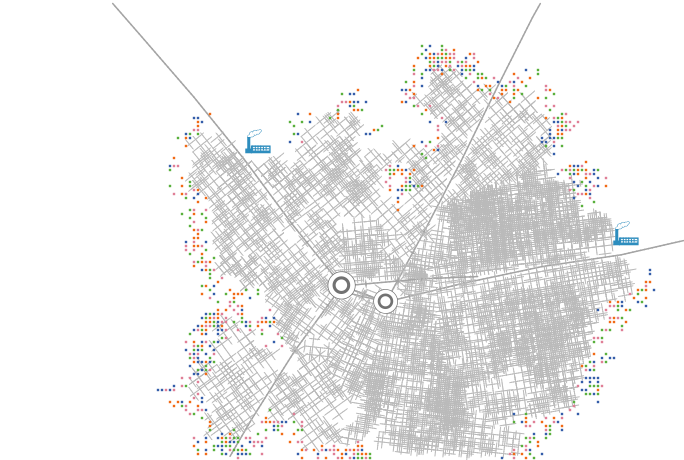
\includegraphics[width=0.3\linewidth]{Figures/Reproducibility/stdView}
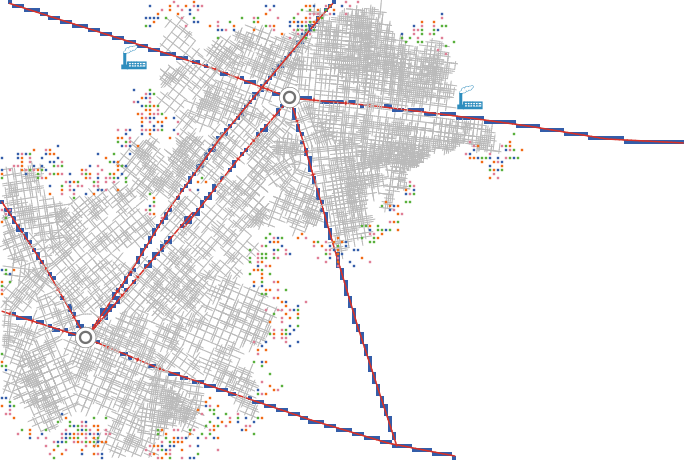
\includegraphics[width=0.3\linewidth]{Figures/Reproducibility/ViewRoads}
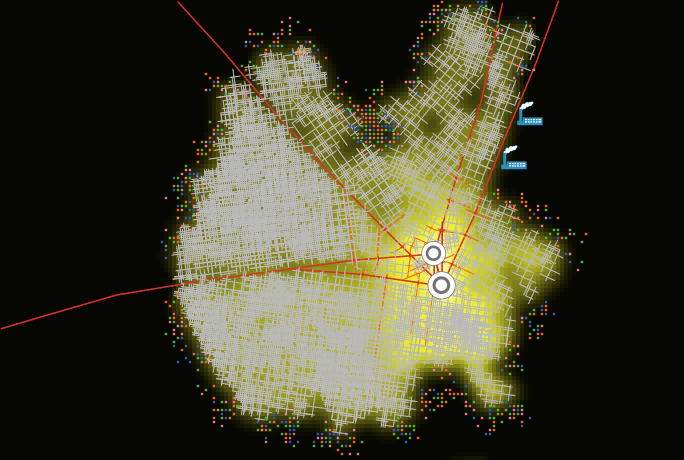
\includegraphics[width=0.3\linewidth]{Figures/Reproducibility/landValues_cityFinished}

\caption[Reproducibility and visualization][Reproductibilité et visualisation]{Example of simple improvement in visualization that can help understanding mechanisms implied in the model. \textit{Left: } Example of original output ; \textit{Middle: } Visualization of main roads (in red) and underlying patches attribution, suggesting possible implementation bias in the use of discretized trace of roads to track their positions ; \textit{Right: }Visualization of land values using a more readable color gradient. This step confirms the hypothesis, through the form of value distribution, that the morphogenesis step is an unnecessary detour to generate a random field for which simple diffusion method should provide similar results, as detailed in the paragraph on implementation.\label{fig:example_tij_viz}}{\textbf{Exemple d'amélioration simple dans la visualisation qui peut aider à appréhender les mécanismes impliqués par le modèle.} (Gauche) Exemple de sortie originale ; (Centre) Visualisation des routes principales (en rouge) et de l'attribution des patches sous-jacente, qui suggère de possibles biais d'implémentation dans l'utilisation de la trace discrete des routes pour garder trace de leur position ; (Droite) Visualisation des valeurs foncières en utilisant un gradient de couleur plus lisible. Cette étape confirme l'hypothèse, par la forme de la distribution des valeurs, que l'étape de morphogenèse est un détour non-nécessaire pour générer un champ aléatoire pour lequel des simples mécanismes de diffusion devrait fournir des résultats similaires, comme détaillé dans le paragraphe sur l'implémentation. Initialement, l'interface du modèle ne permet pas ces options de visualisation, ces à dire se limite à la première image. On ne peut se rendre compte des processus en jeu pour la morphogenèse, liés aux patches de route et au valeurs foncières se diffusant.\label{fig:reproducibility:example_tij_viz}}
\end{figure}
%%%%%%%%%%%%%%%%%%%%%



%%%%%%%%%%%%%%%%%%%%%
\subsubsection{On the Need of Exactitude in Model Implementation}{Sur le besoin d'exactitude dans l'implémentation du modèle}


\bpar{
Possible divergences between model description in a paper and the effectively implemented processes may have grave consequences on the final reproducibility. The road network growth model given in~\cite{barthelemy2008modeling} is one example of such a discrepancy. A strict implementation of model mechanisms provide slightly different results than the one presented in the paper, and as source code is not provided we need to test different hypotheses on possible mechanisms added by the programmer (that seems to be a connexion rule to intersections under a certain distance threshold). Lessons that could be possibly drawn from this examples are 
\begin{itemize}
\item the necessity of providing source code
\item the necessity of providing architecture description along with code (if model description is in a langage too far from architectural specifications) in order to identify possible implementation biaises
\item the necessity of performing and detailing explicitly model explorations, that would in that case have helped to identify the implementation bias.
\end{itemize}
}{
Des divergences potentielles entre la description du modèle dans un article et les processus effectivement implémentés peut avoir des conséquences graves sur la reproductibilité finale. Le modèle de croissance du réseau routier donné dans~\cite{barthelemy2008modeling} est un exemple d'un tel décalage. Une implémentation stricte des mécanismes du modèle produit des résultats légèrement différents de ceux présentés dans le papier, et comme le code source n'est pas fourni nous devrions tester différentes hypothèses sur des mécanismes possibles ajoutés par le programmeur (qui semble être une règle de connexion aux intersections sous un certain seuil de distance). Des leçons qui peuvent éventuellement être tirées de cet exemple, qui rejoignent partiellement mais complètent celle tirées dans l'étude de cas précédente, sont
\begin{itemize}
\item la nécessité de fournir le code source
\item la nécessité de fournir une description de l'architecture en même temps que le code (si la description du modèle est faite dans un langage trop loin de spécification architecturales) afin d'identifier des biais possibles d'implémentation
\item la nécessité de procéder à des explorations explicites du modèle et de les détailler, ce qui dans ce cas aurait permis d'identifier de possibles biais d'implémentation.
\end{itemize}
}



\bpar{
Making the last point mandatory may ensure a limited risk of scientific falsification as it is generally more complicated to fake false exploration results than to effectively explore the model. One could imagine an experiment to test the general behavior of a subset of the scientific community regarding reproducibility, that would consist in the writing of a false modeling paper in the spirit of~\cite{zilsel2015canular}, in which opposite results to the effective results of a given model are provided, without providing model implementation. A first bunch of test would be to test the acceptance of a clearly non-reproducible paper in diverse journals, possibly with a control on textual elements (using or not ``buzz-words'' associated to the journal, etc.). Depending on results, a second experiment may be tested with providing open source code for model implementation but still with false results, to verify if reviewers effectively try to reproduce results when they ask for the code (in reasonable computational power limits of course, HPC being not currently broadly available in Humanities).
}{
Rendre le dernier point obligatoire pourrait assurer un risque limité de falsification puisqu'il est généralement plus compliqué de falsifier des résultats d'exploration plutôt que d'explorer effectivement le modèle. On pourrait imaginer une expérience pour tester le comportement général d'un sous-ensemble de la communauté scientifique au regard de la reproductibilité, qui consisterait en l'écriture d'un faux papier de modélisation dans l'esprit de \cite{zilsel2015canular}, dans lesquels des résultats opposés aux résultats effectifs d'un modèle donné seraient fournis, sans fournir l'implémentation du modèle. Un premier test serait de tester l'acceptation d'un papier clairement non reproductible dans divers journaux, si possible avec un contrôle sur les éléments textuels (par exemple en utilisant ou non des ``buzz-words'' chers au journal). Selon les résultats, une expérience plus poussée serait de fournir l'implémentation open source mais toujours avec des résultats modifiés plus ou moins fortement, afin de tester si les reviewers essayent effectivement de reproduire les résultats quand ils demandent le code (dans des capacités de calcul limitées bien sûr, le HPC n'étant pas encore largement disponibles en sciences sociales). Notre intuition est que les résultats obtenus seraient fortement négatifs, vu les difficultés rencontrées par une exigence de discipline de reproduction indépendante lors de nombreuses relectures, même pour des revues faisant de la reproductibilité une condition \emph{sine qua non} de la publication, les auteurs trouvant des astuces pour se dérober aux contraintes (postuler que des données de simulation ne sont pas des données, ne fournir qu'une version agrégée inutile du jeu de données utilisées, etc. ; nous reviendrons sur le rôle des données plus loin).
}






%%%%%%%%%%%%%%%%%%%%%
\subsection{Interactive Exploration and Production of Results}{Exploration interactive et production des résultats}

L'usage d'applications interactives pour la fouille de données a des avantages non discutables, tel qu'une familiarisation avec la structure des données par une vue d'ensemble qui serait beaucoup plus laborieuse voire impossible autrement. C'est la même idée sous-jacente qui justifie l'interactivité pour l'exploration préliminaire des modèles basé-agent intégrée à des plateformes comme Netlogo~\cite{wilensky1999netlogo} ou Gamma [Cit. gamma]. C'était d'ailleurs un objectif couplé qu'avait initialement~\cite{rey2015plateforme}, c'est à dire une intégration complète de l'exploration fine des modèles et de la production des graphes de sortie ainsi que leur exploration interactive. Comme le rappelle R. Reuillon (Entretien du 11/04/2017, voir \ref{app:data:interview}), la plateforme OpenMole qui devait accueillir cette couche supplémentaire était à ses débuts à l'époque et ne l'est toujours pas aujourd'hui, puisque l'état de l'art de telles pratiques est en pleine construction et bouleversements réguliers~\cite{holzinger2014knowledge}. Des difficultés au regard de la reproductibilité, qui nous concernent particulièrement ici, sont récurrentes et loin d'être résolues. En effet, il faut bien situer la position de ces outils et méthodes comme une aide cognitive préliminaire\footnote{que nous ne jugeons pas superficielle puisque nous les mobilisons au moins par deux fois par la suite, voir \ref{sec:transportationequilibrium} et \ref{sec:energyprice}}, mais peu souvent comme permettant la production de résultats finaux : lorsque les paramètres ou dimension se multiplient, l'export d'un graphe est bien souvent déconnecté de l'information complète ayant conduit à sa production. De la même manière, l'utilisation de notebooks intégrés tel Jupyter, permettant d'intégrer analyses et rédaction du compte-rendu, peut devenir dangereux car on peut justement revenir sur un script, tester différentes valeurs d'un paramètre, et perdre les valeurs qui avaient produit un graphe donné. L'utilisation de versioning peut être une solution partielle mais souvent lourde. Dans l'idéal, tout logiciel interactif permettant l'export de résultats devrait en même temps exporter un script ou une description exacte et utilisable permettant d'arriver exactement à ce point à partir des données brutes. La plupart des applications d'exploration interactives de données spatio-temporelles sont à ce regard relativement immatures scientifiquement, car même dans le cas où elles sont totalement honnêtes et transparentes sur les analyses présentées à l'utilisateur, ce qui n'est malheureusement pas la règle, les tâtonnements d'exploration progressive ne sont pas reproductibles et la méthode d'extraction de caractéristiques est ainsi relativement aléatoire. En poussant le raisonnement, leur utilisation révélerait plutôt l'aveu d'une faiblesse d'un manque de méthodes systématiques accompagnant la découverte de motifs dans des données spatio-temporelles complexes de manière efficace. De manière très visionnaire, \noun{Banos} avait déjà mis en garde contre ``les dangers de la jungle'' des données dans~\cite{banos2001propos}, quand il souligne très justement que l'exploration interactive doit nécessairement se doubler d'indicateurs locaux adaptés, mais surtout d'outils d'exploration automatisés et de critère d'évaluation des choix faits et des motifs découverts par l'utilisateur. On revient encore à l'idée d'une plateforme intégrée dont OpenMole pourrait être un précurseur. La combinaison des capacités cognitives humaines au traitement machine, notamment pour des problèmes de vision par ordinateur, ouvre des possibilités de découvertes inédites, encore plus via une utilisation collective comme en témoigne le Galaxy Zoo~\cite{2010AEdRv...9a0103R}. Les résultats d'un crowdsourcing de la cognition humaine peuvent rivaliser avec les techniques automatiques les plus avancées comme le montre~\cite{10.1371/journal.pone.0178165} pour l'exemple de la comparaison de cartes spatiales. Ces possibilités ne doivent cependant pas être sur-estimées ou utilisées à mauvais escient, et les questions d'intégration efficiente homme-machine sont d'ailleurs totalement ouvertes. Dans le domaine de la visualisation de l'information géographique, \cite{pfaender2009spatialisation} introduit une sémiologie spécifique visant à favoriser l'exploration de grands jeux de données hétérogènes, et l'expérimente sur une application spécifique : il s'agit d'une avancée considérable vers une plateforme intégrée et une exploration interactive saine et reproductible, les directions d'exploration répondant à des modèles basés sur les sciences cognitives. 






%%%%%%%%%%%%%%%%%%%%%
\subsection{Perspectives}{Perspectives}


\bpar{
Again, reproducibility and transparency is a non-negotiable feature of contemporaneous science, along with Open practices and Open Access. Too much examples (see a very recent one in experimental economics~\cite{camerer2016evaluating}) show in various disciplines the lack of reproducibility of experiments, that is a falsification of previous results or a result in itself. Falsification is a costly practice, and even if necessary~\cite{chavalarias2005nobel}, could be made more efficient through more transparency and direct reproducibility, increase therein the global workflow of science. We develop in parallel of this thesis various tools aimed to ease reproducibility, for which an overview is given in appendix~\ref{app:workflow}.
}{
Encore une fois, la reproductibilité et la transparence sont des éléments essentiels incontournables de la science contemporaine, liés aux pratiques de science ouverte et d'accès ouvert. Beaucoup d'exemples (voir un récent en économie expérimentale dans~\cite{camerer2016evaluating}) dans diverses disciplines montrent le manque de reproductibilité des résultats des expériences, alors que celle ci doit pouvoir conduire à une falsification ou à une confirmation de ces résultats. La falsification est une pratique coûteuse car demandant un certain investissement au détriment de sa propre recherche~\cite{chavalarias2005nobel}. Elle pourrait ainsi être rendue plus efficiente grâce à une transparence augmentée. Des outils spécialement dédiés à une reproductibilité directe, souvent permise par l'ouverture, devraient accroître la performance globale de la science. Mais l'accès ouvert a des impacts bien plus large que la science elle-même : \cite{2015arXiv150607608T} montre un transfert des connaissances scientifiques accru vers la société dans le cas d'articles ouverts, notamment par des intermédiaires comme Wikipedia.
}

Le développement et la systématisation de standards et de bonnes pratiques, de manière conjointe sur les différentes problématiques évoquées, est une condition nécessaire à une rigueur scientifique qui devrait être uniforme au travers de l'ensemble des disciplines existantes. Nous construisons par exemple des exemples d'outils facilitant le flot de production scientifique, ceux-ci étant détaillés en Appendice~\ref{app:workflow}. Par exemple, pour les sciences computationnelles, on a déjà évoqué les potentialités de l'utilisation de \texttt{git} qui s'étendent en fait sans contrainte de disciplines ni de types de recherche si les bonnes adaptations sont introduites. Le suivi précis de l'ensemble des étapes d'un projet, gardé en historique offrant la possibilité de revenir à n'importe laquelle à tout moment, mais aussi de travailler de façon collaborative, plus ou moins parallèlement selon les besoins en utilisant les branches, est un exemple de service fourni par cet outil. Un exemple de bonnes pratiques d'utilisation est donné par~\cite{10.1371/journal.pcbi.1004947}. Plus généralement, les sciences computationnelles nécessitent l'adoption de certains standards et pratiques pour assurer une bonne reproductibilité, et ceux-ci restent majoritairement à développer : \cite{wilson2017good} donne des premières pistes. Concernant la qualité des données, de nombreux efforts sont faits pour introduire des cadres de standardisation des données : par exemple~\cite{10.1371/journal.pone.0178731} décrit un cadre conceptuel visant à guider la résolution de problème récurrent liés à la qualité des données de biodiversité (comme par exemple évaluer des mesures jugeant de l'usage possible d'un jeu de données pour un problème donné).

\comment{citer Romain sur le blockchain, en lien avec ce papier ? \cite{2017arXiv170706552}}


L'accès aux données est également un point crucial pour la reproductibilité, et sans nous y attarder car cela impliquerait des développements sur la définition, la philosophie, le droit des données etc. qui sont des sujets de recherche en eux-même, nous donnons des perspectives sur les potentiels d'une ouverture systématique des données en recherche. En géographie, les \emph{data paper} sont une pratique inexistante, et la règle est plutôt de garder la main jalousement sur un jeu produit, capitalisant sur le fait d'être le seul à y avoir accès. Il est évident que la qualité et quantité des connaissances produites sera nécessairement plus grande si un jeu de données est publiquement ouvert, puisqu'au moins la même chose sera obtenue, et on peut s'attendre à une prise en main par d'autres domaines, d'autres méthodes, et donc à une plus grande richesse. La fermeture induira plutôt des effets négatifs, comme par exemple du temps perdu à recoder un base vectorielle donnée uniquement sous forme de carte dans un article. L'argument du temps passé comme justification à la fermeture est absurde, puisqu'au contraire, en voyant les données comme une composante à part entière de la connaissance (voir le cadre de connaissances en~\ref{sec:knowledgeframework}), le temps passé doit impliquer plus de citations, donc plus d'utilisation, ce qui passe nécessairement par l'ouverture pour des données. De même, quelle logique, sinon la même absurde de propriété des connaissances, pousse les géographes à insérer un copyright sur l'ensemble de leurs cartes mais aussi leurs figures, jusqu'à un copyright pour un simple histogramme qui s'en serait bien passé si on avait pu l'interroger, honnête de simplicité ? Une expérience de revue induit à réellement s'inquiéter sur la valeur donnée à l'ouverture des données par les auteurs : au bout d'une dizaine d'articles, incluant des journaux affichant comme priorité et pré-requis l'ouverture totale des données et modèles, dont un seul est seulement partiellement ouvert et l'ensemble des autres implique de croire sur parole les résultats présentés (alors qu'un des but de la revue est de contourner les biais cognitifs qu'un ou des humains ont forcément par une validation croisée qui doit se faire sur les résultats bruts et non des interprétations contenant ces biais), il est difficile de croire que des mutations profondes des pratiques ne sont pas nécessaire. Mais en suivant l'adage de Framasoft, ``la route est longue mais la voie est libre'', les perspectives sont nombreuses pour une évolution dont la lenteur n'est pas inéluctable. Le journal Cybergéo, pionnier des pratiques d'ouverture en sciences sociales (première revue entièrement électronique, première revue à lancer une rubrique de \emph{model papers}), lance en 2017 une rubrique \emph{data papers} visant à inciter le développement du partage de données et de l'ouverture en géographie. Il reste des zones grises sur lesquelles il est impossible aujourd'hui d'avoir des perspectives, notamment le droit des données. On peut citer des exemples parmi les études empiriques que nous développons : les données bibliographiques sont obtenues au prix d'une guerre de blocage par Google et un effort considérable pour la gagner ; les données immobilières proviennent d'une base propriétaire achetée avec de l'argent public, et nous pouvons profiter d'un flou du contrat pour les rendre disponibles de manière agrégées avec les résultats ; les données des stations essence proviennent d'une source dont la légalité ne devrait pas être creusée plus, et nous ne pouvons malheureusement pas les rendre disponibles sans prendre de risques - cet aspect n'a cependant jamais fait broncher les reviewers qui n'ont même pas mentionné le manque d'accès aux données. L'ouverture implique un engagement qui fait résolument partie de nos positionnements. C'est la même idée qui soutient la construction de l'application \texttt{CybergeoNetworks}\footnote{\texttt{http://shiny.parisgeo.cnrs.fr/CybergeoNetworks}}, qui couple les outils présentés en~\ref{sec:quantepistemo} avec d'autres approches complémentaires d'analyse de corpus, dans le but d'encourager la réflexivité scientifique, et de mettre cet outil ouvert à la disposition d'éditeurs indépendants, pour s'émanciper de la nouvelle main mise des géants de l'édition qui à la recherche d'un nouveau modèle pour sécuriser leur profits parient sur la vente de meta-contenu et de son analyse. Heureusement, la récente loi numérique en France a gagné le bras de fer contre leur revendication d'un droit exclusif sur la fouille de texte complets.

%inserer lien vers residential dynamics repo ? % NON

% crowdsourcing / opendata : https://sci-hub.cc/https://www.nature.com/nature/journal/vaop/ncurrent/full/nature24621.html# microbial dna base



\stars



% 3.2 Big Data, Computation and Model Exploration





%----------------------------------------------------------------------------------------

\newpage



%\section[Computation and Model Exploration][Calcul Intensif et Exploration des Modèles]{Big Data, Computation and Model Exploration}{Données Massives, Calcul Intensif et Exploration des Modèles}
\section{Modeling, Big Data and Computation}{Modélisation, données massives et calcul intensif}


\label{sec:computation}


%----------------------------------------------------------------------------------------



Nous nous positionnons à présent sur les questions liées à l'utilisation des données massives et du calcul intensif, ce qui induit par extension une réflexion sur les méthodes d'exploration de modèles. Il n'est pas évident que ces nouvelles possibilités soient nécessairement accompagnées de mutations épistémologiques profondes, et nous montrons au contraire que leur utilisation nécessite plus que jamais un dialogue avec la théorie. Implicitement, cette position préfigure le cadre épistémologique pour l'étude des Systèmes Complexes dont nous donnons le contexte à la section suivante~\ref{sec:epistemology} et que nous formalisons en ouverture~\ref{sec:knowledgeframework}.




%----------------------------------------------------------------------------------------



%%%%%%%%%%%%
\subsection{Why modeling ?}{Pourquoi modéliser ?}









\subsubsection{Link between modeling and Open Science}{Lien entre modélisation et Science Ouverte}



\bpar{
The last methodological point which we need to emphasis is the relation between the workflow we introduce and model exploration workflows. The ideas of multi-modeling and extensive model exploration are nothing from new as Openshaw already advocated for ``model-crunching'' in~\cite{openshaw1983data}, but their effective use only begins to emerge thanks to the apparition of new methods and tools together with an explosion of computation capabilities: \cite{cottineau2016back} claims for a renewed approach on multi-modeling. Coupling models as we do answers to similar questions. In that stream of research, the model exploration platform OpenMole~\cite{reuillon2013openmole} allows to embed any model as a blackbox, write modulable exploration workflow using advanced methodologies such as genetic algorithms and distribute transparently the computation on large scale computation infrastructures such as clusters or computation grids. In our case, the workflow tool is a powerful way to embed both the sensitivity analysis and the meta-sensitivity analysis, and allow to couple any generator with any model in a straightforward way as soon as the model can take its spatial configuration as input or from an input file.
}{
Enfin, il est important de souligner brièvement les liens entre pratiques de modélisation et science ouverte, comme le lien entre reproductibilité et Science Ouverte souligné à la fin de~\ref{sec:reproducibility}. En fait, la Science Ouverte est composée d'un ensemble de pratiques se déclinant sur différents domaines, d'où sa ventilation logique dans nos positionnements. Pour illustrer les enjeux, nous proposons de décrire l'exemple des workflows d'exploration de modèle comme une méthode de meta-analyse de sensibilité, c'est à dire un aspect de la méthodologie appliquée ci-dessus. Les idées de multi-modélisation et d'exploration intensive de modèle sont tout sauf nouvelles puisque \noun{Openshaw} défendait déjà le ``model-crunching'' dans~\cite{openshaw1983data}, mais leur utilisation effective commence seulement à émerger grâce à l'apparition de nouvelles méthodes et outils en même temps qu'une explosion des capacités de calcul : \cite{cottineau2016back} propose une approche renouvelée de la multi-modélisation. Le couplage de modèles tel que nous l'opérons répond à des questions similaires. Dans cette lignée de recherche, la plateforme d'exploration de modèle OpenMole~\cite{reuillon2013openmole} permet d'embarquer n'importe quel modèle comme une boîte noire, d'écrire des workflow d'exploration modulables qui utilisent des méthodologies d'exploration avancées comme des algorithmes génétiques, et de distribuer de manière transparente les calculs sur des infrastructures de calcul à grande échelle comme des clusters ou grilles de calcul. Dans le cas précédent, l'outil du workflow est un outil puissant pour intégrer à la fois l'analyse de sensibilité et la meta-analyse de sensibilité, et permet de coupler n'importe quel générateur avec n'importe quel modèle de façon très directe tant que le modèle peut prendre la configuration spatiale \comment[AB]{?} comme entrée ou dans un fichier d'entrée. D'autre part, une idée des workflow est de favoriser des constructions ouvertes et collaboratives, puisque le ``marketplace'' d'OpenMole, directement intégré au logiciel, permet de bénéficier directement des exemples qui auront été partagés sur le dépôt collaboratif. Cela ressemble aux plateformes de partage de modèles, qui sont nombreuses pour les modèles agents par exemple, mais dans un esprit encore plus modulaire et participatif. Ainsi, certains choix épistémologiques et méthodologiques au regard de la modélisation impliquent directement un positionnement au regard de la science ouverte : la multi-modélisation et les familles de modèles, qui vont de pair avec le couplage de modèle hétérogènes et multi-échelles, ne peuvent guère être viables sans des pratiques d'ouverture, de partage et de construction collaborative des modèle, comme le rappelle~\cite{banos2013pour}.
}

\comment{Sur la pédagogie : \cite{chen2006effectiveness} : la simulation comme outil pour apprendre aux élèves ingénieurs. Intéressant à utiliser pour l'aspect performatif, feedback des modèles sur les situations réelles / illustration des différents objectifs de chaque domaine : pourquoi et comment c'est intéressant de prendre en compte certains aspects selon les objectifs / perspectivisme appliqué : faire ce projet , l'évoquer ici.}







%----------------------------------------------------------------------------------------


%%%%%%%%%%%%%%
\subsection{For a cautious use of big data and computation}{Pour un usage raisonné des données massives et de la computation}

\bpar{
The so-called \emph{big data revolution} resides as much in the availability of large datasets of novel and various types as in the always increasing available computational power. Although the \emph{computational shift} (\cite{arthur2015complexity}) is central for a science aware of complexity and is undeniably the basis of future modeling practices in geography as \cite{banos2013pour} points out, we argue that both \emph{data deluge} and \emph{computational potentialities} are dangerous if not framed into a proper theoretical and formal framework. The first may bias research directions towards available datasets (as e.g. numerous twitter mobility studies) with the risk to disconnect from a theoretical background, whereas the second may overshadow preliminaries analytical resolutions essential for a consistent use of simulations. We argue that the conditions for most of results in this thesis are indeed the ones endangered by incautious big-data enthusiasm, concluding that a main challenge for future Geocomputation is a wise integration of novel practices within the existing body of knowledge.
}{
La soi-disante \emph{révolution des données massives} réside autant dans la disponibilité de grands jeux de données de nouveaux types variés, que dans la puissance de calcul potentielle toujours en augmentation. Même si le \emph{tournant computationnel} (\cite{arthur2015complexity}) est central pour une science consciente de la complexité et est sans douter la base des pratiques de modélisation futures en géographie comme \cite{banos2013pour} souligne, nous soutenons que à la fois le \emph{déluge de données} et les \emph{capacités de calcul} sont dangereuses si non cadrées dans un cadre théorique et formel propre. Le premier peut biaiser les directions de recherche vers les jeux de données disponibles avec le risque de se déconnecter d'un fond théorique, tandis que le second peut occulter des résolutions analytiques préliminaires essentielles pour un usage cohérent des simulations. Nous avançons que les conditions pour la majorité des résultats dans cette thèse sont en effet ceux mis en danger par un enthousiasme inconsidéré pour les données massives, tirant la conclusion qu'un challenge majeur pour la géocomputation future est une intégration sage des nouvelles pratiques au sein du corpus existant de connaissances.
}


\bpar{
The computational power available seems to follow an exponential trend, as some kind of Moore's law. Both effective Moore's law for hardware, and improvement of softwares and algorithms, combined with a democratization of access to large scale simulation facilities, makes always more and more CPU time available for the social scientist (and to the scientist in general but this shift happened quite before in other fields, as e.g. CERN is leading in cloud computing and grid computation). About 10 years ago, \cite{gleyze2005vulnerabilite} concluded that network analysis, for the case of Parisian public transportation network, was ``limited by computation''. Today most of these analyses would be quickly done on a personal computer with appropriated software and coding: \cite{2015arXiv151201268L} is a witness of such a progress, introducing new indicators with a higher computational complexity, computed on larger networks. The same parallel can be done for the Simpop models: the first Simpop models at the beginning of the millenium~\cite{sanders1997simpop} were ``calibrated'' by hand, whereas \cite{cottineau2015modular} calibrates the multi-modeling Marius model and~\cite{schmitt2014half} calibrates very precisely the SimpopLocal model, both on grid with billions of simulations. A last example, the field of Space Syntax, witnessed a long path and tremendous progresses from its theoretical origins~\cite{hillier1989social} to recent large-scale applications~\cite{hillier2016fourth}.
}{
La puissance de calcul disponible semble suivre un tendance exponentielle, comme une sorte de loi de Moore. Grace à d'une part la loi de Moore effective pour le matériel, d'autre part l'amélioration des logiciels et algorithmes, conjointement avec une démocratisation de l'accès au infrastructures de simulation à grande échelle, permet à toujours plus de temps processeur d'être disponible pour le chercheur en sciences sociales (et pour le scientifique en général, mais cette mutation a déjà été opérée depuis plus longtemps dans d'autres domaines%, puisque par exemple le CERN est à la pointe en terme de calcul distant et sur grille % exemple déjà utilisé
). Il y a environ une dizaine d'année, \cite{gleyze2005vulnerabilite} était forcé de conclure que les analyses de réseau, pour les transports publics parisiens, étaient ``limitées par le calcul''. Aujourd'hui la plupart des mêmes analyses seraient rapidement réglée sur un ordinateur personnel avec les logiciels et programmes appropriés : \cite{2015arXiv151201268L} est un témoin d'un tel progrès, introduisant des nouveaux indicateurs avec une plus grande complexité de calcul, qui sont calculés sur des réseaux à grande échelle. Le même parallèle peut être fait pour les modèles Simpop : les premiers modèles Simpop au début du millénaire~\cite{sanders1997simpop} étaient ``calibrés'' à la main, tandis que \cite{cottineau2015modular} calibre le modèle Marius en multi-modélisation et~\cite{schmitt2014half} calibre très précisément le modèle SimpopLocal, chacun sur la grille avec des milliards de simulations. Un dernier exemple, le champ de la \emph{Space Syntax}, a témoigné d'une longue route et de progrès considérables depuis ses origines théoriques~\cite{hillier1989social} jusqu'à ses récentes applications à grande échelle~\cite{hillier2016fourth}.
}



\bpar{
Concerning the new and ``big'' data available, it is clear that always larger dataset are available and always newer type of data are available. Numerous examples of fields of application can be given. For example, mobility can now be studied from various entries, such as new data from smart transportation systems~\cite{o2014mining}, from social networks~\cite{frank2014constructing}, or other more exotic data such as mobile phone data~\cite{de2016death}. In an other spirit, the opening of ``classic'' datasets (such as city dashboards, open data government initiatives) should allow ever more meta-analyses. New ways to do research and produce data are also raising, towards more interactive and crowd-sourced initiatives. For example, \cite{2016arXiv160606162C} describes a web-application aimed at presenting a meta-analysis of Zipf's law across numerous datasets, but in particular features an upload option, where the user can upload its own dataset and add it to the meta-analysis. Other applications allow interactive exploration of scientific literature for a better knowledge of a complex scientific landscape, as~\cite{cybergeo20} does.
}{
Concernant les nouvelles données ``massives'' qui sont disponibles, il est clair que des quantités toujours plus grandes et des types toujours nouveaux sont disponibles. De nombreux exemples de champs d'application peuvent être donnés. La mobilité en est typique, puisque étudiée selon divers points de vue, comme les nouvelles données issues des systèmes de transport intelligents~\cite{o2014mining}, des réseaux sociaux~\cite{frank2014constructing}, ou des données plus exotiques comme des données de téléphonie mobile~\cite{de2016death}. Dans un autre esprit, l'ouverture de jeux de données ``classiques'' (comme les applications synthétiques urbaines, les initiatives gouvernementales pour les données ouvertes) devrait pouvoir toujours plus de méta-analyses. De nouvelles façon de pratiquer la recherche et produire des données sont également en train d'émerger, vers des initiatives plus interactives et venant de l'utilisateur. Ainsi, \cite{2016arXiv160606162C} décrit une application web ayant pour but de présenter une méta-analyse de la loi de Zipf sur de nombreux jeux de données, mais en particulier inclut une option de dépôt, à travers laquelle l'utilisateur peut télécharger sont propre jeu de données et l'inclure dans la méta-analyse. D'autres applications permettent l'exploration interactive de la littérature scientifique pour une meilleure connaissance d'un horizon scientifique complexe, comme~\cite{cybergeo20} fait.
}


\bpar{
As always the picture is naturally not as bright as it seems to be at first sight, and the green grass that we try to go eating in the neighbor's field quickly turns into a sad reality. Indeed, the purpose and motivation are fuzzy and one can get lost. Some examples speaks for themselves. \cite{barthelemy2013self} introduces a new dataset and rather new methods to quantify road network evolution, but the results, on which the authors seem to be astonished, are that a transition occurred in Paris at the Haussmann period. Any historian of urbanism would be puzzled by the exact purpose of the paper, as in the end a vague and bizarre feeling of reinventing the wheel floats in the air. The use of computation can also be exaggerated, and in the case of agent-based modeling it can be illustrated by the example of~\cite{axtell2016120}, for which the aim at simulating the system at scale 1:1 seems to be far from initial motivations and justifications for agent-based modeling, and may even give arguments to mainstream economists that denigrate easily ABMS. Other anecdotes raise worries: \cite{robin_cura_2014_11415} is a web application that wastes computational ressources to simulate Gaussian distributions for a Gibrat model in order to compute their mean and variance, that are input parameters of the model. It basically checks the Central Limit Theorem, which is a priori well accepted among most scientists. Otherwise, the full distribution given by a Gibrat model is theoretically known as it was fully solved e.g. by \cite{gabaix1999zipf}. Recently on the French speaking diffusion list \emph{Geotamtam}, a sudden rush around \emph{Pokemon Go} data seemed to answer more to an urgent unexplained need to exploit this new data source before anyone else rather than an elaborated theoretical construction. Simple existing accurate datasets, such as historical cities population (for France the Pumain-INED database for example), are far from being fully exploited and it may be more important to focus on these already existing classic data. One must also be aware of the possible misleading applications of some results: \cite{louail2016crowdsourcing} makes a very good analysis of potential redistribution of bank card transactions within a city, but pushes the results as possible basis for social equity policy recommandation by acting on mobility, forgetting that urban form and function are coupled in a complex way and that moving transactions from one place to the other involves far more complex processes than policies.
}{
Comme toujours la situation n'est naturellement pas aussi idyllique qu'elle semble être au premier abord, et l'herbe verte du pré du voisin que nous pouvons être tentés d'aller brouter se transforme rapidement en un triste fumier. En effet, les objectifs et motivations sont flous et on peut facilement s'y perdre. Des illustrations parleront d'elles-même. \cite{barthelemy2013self} introduit un nouveau jeu de données et des méthodes relativement nouvelles pour quantifier l'évolution du réseau de rues, mais les résultats, sur lesquels les auteurs semblent s'étonner, sont qu'une transition a eu lieu à Paris à l'époque d'Haussmann. Tout historien de l'urbanisme s'interrogerait sur le but exact de l'étude, puisque à la fin un sentiment étrange de réinvention de la roue flotte dans l'air. L'utilisation des ressources de calcul peut également être exagéré, et dans le cas de la modélisation multi-agent, on peut citer~\cite{axtell2016120}, pour lequel l'objectif de simuler le système à l'échelle 1:1 semble être loin des motivations et justifications originelles de la modélisation agent, et pourrait même donner des arguments aux économistes \emph{mainstream} qui dénigrent facilement les ABMS. D'autres anecdotes peuvent inquiéter :  il existe en ligne des exemples étonnants, comme une application web\footnote{voir http://shiny.parisgeo.cnrs.fr/gibratsim/} qui utilise des ressources de calcul financées par l'argent public pour simuler des distributions Gaussiennes afin de calculer pour un modèle de Gibrat, afin de calculer leur moyenne et variance, qui sont des paramètres d'entrée du modèle. En résumé, cela revient à vérifier le Théorème de la Limite Centrale. D'autre part, la distribution complète donnée par un modèle de Gibrat est entièrement connue théoriquement comme résolu e.g. par~\cite{gabaix1999zipf}. Sur ce point, nous devons partiellement être en désaccord avec le neuvième commandement de \noun{Banos}, qui rappelle que ``les mathématiques ne sont pas le language universel des modèles'', ou plutôt souligner les dangers d'une mauvaise interprétation de ce principe\footnote{De manière générale, les commandements de \noun{Banos} paraissent simples dans leur formulation, mais sont d'une profondeur et d'une complexité déconcertante lorsqu'on essaye d'en tirer les implications et la philosophie globale sous-jacente, et ne doivent jamais être pris à la légère.} : il postule que des moyens alternatifs aux mathématiques existent pour faire comprendre des processus ou des méthodes, mais précise que ceux-ci sont une porte d'entrée et ne prétend jamais qu'il est possible de se passer des mathématiques, dérive que l'exemple précédent illustre parfaitement. D'ailleurs, il est possible d'exhiber des structures mathématiques très simples, comme un simplexe en dimension quelconque, dont la visualisation ``simple'' est un problème ouvert. Les données fournissent aussi leur collection de dérives. Récemment, sur la liste de diffusion de géographie francophone \emph{Geotamtam}, un soudain engouement autour des données issues de \emph{Pokemon Go} a semblé répondre plus à un besoin urgent et inexpliqué d'exploiter cette source de données avant tous les autres, plutôt qu'à des considérations théoriques élaborées. Des jeux de données existant et précis, comme la population historiques des villes (pour la France la base Pumain-INED par exemple), sont loin d'être entièrement exploités et il pourrait être plus pertinent de se concentrer sur ces jeux de données classiques qui existent déjà. De même, il faut être conscient des possibles applications de résultats basée sur des malentendus : \cite{louail2016crowdsourcing} analyse la redistribution potentielle des transactions de carte bancaire au sein d'une ville, mais présente les résultats comme la base possible de recommandations de politiques pour une équité sociale en agissant sur la mobilité, oubliant que la forme et les fonctions urbaines sont couplés de manière complexe et que déplacer des transactions d'un endroit à un autre implique des processus bien plus complexes que des régulations directes, qui d'autant plus ne s'appliquent jamais de la façon prévue et conduisent à des résultats un peu différents. Une telle attitude, souvent observée de la part de physiciens, est très bien mise en allégorie par la figure~\ref{fig:computation:xkcd} qui n'est qu'à moitié une exagération de certaines situations.
}




\bpar{
Our main claim here is that the computational shift and simulation practices will be central in geography, but may also be dangerous, for the reasons illustrated above, i.e. that data deluge may impose research subjects and elude theory, and that computation may elude model construction and solving. A stronger link is required between computational practices, computer science, mathematics, statistics and theoretical geography. Theoretical and Quantitative Geography is at the center of this dynamic, as it was its initial purpose that seems forgotten in some cases. It implies the need for elaborated theories integrated with conscious simulation practices. In other words we can answer complementary naive questions that have however to be tackled one and for once. If a theory-free quantitative geography would be possible, the answer if naturally no as it is close to the trap of black-box data-mining analysis. Whatever is done in that case, the results will have a very poor explanatory power, as they can exhibit relations but not reconstruct processes. On an other hand, the possibility of a purely computational quantitative geography is a dangerous vision: even gaining three orders of magnitudes in computational power does not solve the dimensionality curse. In our work here, without theory, we would not know which objects, measures and properties to look at (e.g. multi-scale and dynamical nature of processes), and without analytics, it would be sometimes difficult to draw conclusions from empirical analysis. Nothing is really new here but this position has to be stated and stood up, precisely because our work will use this kind of tools, trying to advance on a thin and fragile edge, with the void of the unfunded theoretical charlatanism on one side and the abyss of the technocratic blind drowning in foolish amounts of data. More than ever we need simple but powerful and funded theories {\`a}-la-Occam~\cite{batty2016theoretical}, to allow a wise integration of new techniques into existing knowledge.
}{
Notre principal argument est que le tournant computationnel et les pratiques de simulation seront centrales en géographie, mais peuvent également être dangereux, pour les raisons illustrées ci-dessus, i.e. que le déluge de données peut imposer les sujets de recherche et occulter la théorie, et que la computation peut éluder la construction et la résolution de modèles. Un lien plus fort est nécessaire entre les pratiques de calcul, l'informatique, les mathématiques, les statistiques et la géographie théorique. La Géographie Théorique et Quantitative est au centre de cette dynamique, puisqu'il s'agit de sa motivation initiale principale qui semble oubliée dans certains cas. Cela implique un besoin de recherche de théorie élaborées intégrées avec des pratiques de simulation conscientes. En d'autres mots, on peut répondre à des questions naïves complémentaires qui ont toutefois besoin d'être traitées une bonne fois pour toutes. Si une géographie quantitative libérée de la théorie serait possible, la réponse est naturellement non puisque cela se rapproche du piège de la fouille de données par boîte noire. Quoi qu'il soit fait par cette approche, les résultats auront un pouvoir explicatif très faible, puisqu'ils pourront mettre en valeur des relations mais pas reconstruire des processus. D'autre part, la possibilité d'une géographie quantitative purement basée sur le calcul est une vision dangereuse : même le gain de trois ordres de grandeur dans la puissance de calcul disponible ne résout pas le sort de la dimension. Prenons l'exemple des résultats de non-stationnarité obtenus en~\ref{sec:staticcorrelations}. L'utilisation de données relativement massives, de par les algorithmes spécialement conçus pour être capable de faire les traitements, est une condition nécessaire au résultat obtenus, mais à la fois l'échelle est les objets (c'est à dire les indicateurs calculés) sont co-déterminés par les constructions théoriques et les autres études empiriques. En effet l'absence de théorie impliquerait de ne pas connaitre les objets, mesures et propriétés à étudier (e.g. le caractère multi-scalaire ou dynamique des processus), et sans résolutions analytiques, il serait souvent difficile de tirer des conclusions à partir des analyses empiriques seules concernant l'ergodicité par exemple. Rien n'est vraiment nouveau ici mais cette position doit être affirmée et tenue, précisément car notre travail se base sur ce type d'outils, essayant d'avancer sur une arête fine et fragile, avec d'un côté le vide du charlatanisme théorique infondé et de l'autre l'abîme de l'overdose technocratique dans des quantités de données folles. Plus que jamais on a besoin de théories simples mais fondées et puissantes {\`a}-la-Occam~\cite{batty2016theoretical}, pour permettre une intégration saine des nouvelles techniques au sein des connaissances existantes.
}






%%%%%%%%%%%%%%
\begin{figure}
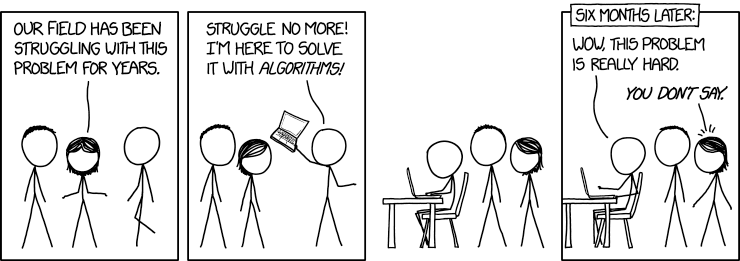
\includegraphics[width=\linewidth]{Figures/Computation/here_to_help}
\caption[Naive use of data mining and computation][Usage naïf de la fouille de données]{On naive use of data mining and intensive computation\label{fig:computation:xkcd}}{De l'usage naïf de la fouille de données et du calcul intensif. Source: \texttt{xkcd}\label{fig:computation:xkcd}}
\end{figure}
%%%%%%%%%%%%%%









%----------------------------------------------------------------------------------------


%%%%%%%%%%%%%%%%%%%%%%
%\subsection[Sensitivity to initial conditions][Sensibilité aux conditions initiales]{Statistical Control on Initial Conditions by Synthetic Data Generation}{Contrôle statistique pour les conditions initiales par génération de données synthétiques}
\subsection{Extend sensitivity analyses}{Etendre les analyses de sensibilité}
	
	

%%%%%%%%%%%%%%%%%%%%%%
\subsubsection{Context}{Contexte}


\bpar{
When evaluating data-driven models, or even more simple partially data-driven models involving simplified parametrization, an unavoidable issue is the lack of control on ``underlying system parameters'' (what is a ill-defined notion but should be seen in our sense as parameters governing system dynamics). Indeed, a statistics extracted from running the model on enough different datasets can become strongly biased by the presence of confounding in the underlying real data, as it is impossible to know if result is due to processes the model tries to translate or to a hidden structure common to all data.
}{
Lors de l'évaluation de modèle basés sur les données, ou même de modèle plus simples partiellement basés sur les données impliquant une paramétrisation simplifiée, une issue inévitable est le manque de contrôle sur les ``paramètres implicites du systèmes'' (ce qui n'est pas une notion stricte mais doit être vu dans notre sens comme les paramètres régissant la dynamique). En effet, une statistique issue d'executions du modèle sur un nombre suffisant d'executions peut toutefois rester biaisée, au sens où il est impossible de savoir si les résultats sont dus aux processus que le modèle cherche à traduire ou à une structure présente dans les données initiale. La question méthodologique fondamentale qui nous intéressera pour la suite est d'être capable d'isoler les effets propres aux processus du modèles de ceux liés à la géographie.
}



\paragraph{Rationale}{Rationelle}


\bpar{
Although simulation models of geographical systems in general and agent-based models in particular represent a fantastic opportunity to explore socio-spatial behaviours and to test a variety of scenarios for public policy, the validity of generative models is uncertain until their results are proven robust. Sensitivity analysis usually include the analysis of the effect of stochasticity on the variability of results, as well as the effects of small parameter changes. However, initial spatial conditions are usually taken for granted in geographical models, thus leaving completely unexplored the effect of spatial arrangements on the interaction of agents and of their interactions with the environment. In this part, we present a method to assess the effect of initial spatial conditions on simulation models, using a systematic generator controlled by meta-parameter to create density grids used in spatial simulation models. We show, with the example of a very classical agent-based model (Sugarscape model of ressource allocation) that the effect of space in simulation is significant, and sometimes even larger than parameters themselves. We do so using high performance computing in a very simple and straightforward open-source workflow. The benefits of this approach are various but include for example the knowledge of model behavior in an extended frame, the possibility of statistical control when regressing model outputs, or a finer exploration of model derivatives than with a direct approach.
}{
Bien que les modèles de simulation des systèmes géographiques en général et les modèles basés-agent en particulier représentent une opportunité considérable d'explorer les comportements socio-spatiaux et de tester une variété de scenarios pour les politiques publiques, la validité des modèles génératifs est incertaine tant que la robustesse des résultats n'a pas été établie. Les analyses de sensibilité incluent généralement l'analyse des effets de la stochasticité sur la variabilité des résultats, ainsi que les effets de variations locales des paramètres. Cependant, les conditions spatiales initiales sont généralement prise pour données dans les modèles géographiques, laissant ainsi totalement inexploré l'effet des motifs spatiaux sur les interactions des agents et sur leur interaction avec l'environnement. Dans cette partie, nous présentons une méthode pour établir l'effet des conditions spatiales initiales sur les modèles de simulation, utilisant un générateur systématique contrôlé par des meta-paramètres pour créer des grilles de densité utilisées dans les modèles de simulation spatiaux. Nous montrons, avec l'exemple d'un modèle agent très classique (le modèle Sugarscape d'extraction de ressources) que l'effet de l'espace dans les simulations est significatifs, et parfois plus grand que l'effet des paramètres eux-mêmes. Nous y arrivons en utilisant le calcul haute performance en un workflow très simple et open source. Les bénéfices de notre approche sont variés mais incluent par exemple la connaissance du comportement du modèle dans un contexte plus large, la possibilité de contrôle statistique pour régresser les sorties du modèles, ou une exploration plus fine des dérivées du modèle que par rapport à une approche directe.
}

\paragraph{Formalization}{Formalisation}


\bpar{
Let first give an abstract formulation of the idea. The generator is considered as an upstream model, coupled simply (outputs become inputs) with the studied downstream model. If $M_u$ is the upstream model, $M_d$ the downstream model and $\alpha$ the meta-parameters, one has the composition of the derivative along the meta-parameter
\[
\partial_{\alpha}\left[M_u \circ M_d\right] = \left(\partial_{\alpha} M_u \circ M_d \right)\cdot \partial_{\alpha} M_d
\]
It implies that the sensitivity of the downstream model to meta-parameters can be determined by studying the serial coupling and the upstream model. We gain some thematic knowledge, in the sensitivity to an implicit meta-parameter, but there is also a computational gain: the generation of controlled differentiates in the ``initial space'' would be complicated to achieve directly. The question of stochasticity in such simply coupled models causes no additional issue as $\Eb{X}=\Eb{\Eb{X|Y}}$. It naturally multiplies the number of repetition needed for convergence what is the expected behavior.
}{
Commençons par donner une formulation abstraite de l'idée, d'un point de vue du couplage de modèle. Le générateur est considéré comme un modèle amont, couplé simplement (les sorties devenant les entrées) avec le modèle aval étudié. Si $M_u$ est le model amont, $M_d$ le modèle aval et $\alpha$ les meta-paramètres, on a la composition de la dérivée le long des meta-paramètres
\[
\partial_{\alpha}\left[M_u \circ M_d\right] = \left(\partial_{\alpha} M_u \circ M_d \right)\cdot \partial_{\alpha} M_d
\]
Cela implique que la sensibilité du modèle aval aux meta-paramètres peut être déterminée en étudiant le couplage séquentiel et le modèle amont. Nous gagnons de la connaissance thématique, dans la sensibilité à un meta-paramètre implicite, mais il y a aussi un gain computationnel : la génération de différentielles contrôlées dans l'espace initial (c'est à dire tester directement la comparaison entre deux grilles proches) serait compliquer à atteindre directement. La question de la stochasticité dans de tels modèles couplés simplement ne pose pas de problème supplémentaire puisque $\Eb{X}=\Eb{\Eb{X|Y}}$. Cela multiplie naturellement le nombre de répétitions pour converger bien évidemment. Nous resterons dans l'application pratique ici à une étude de l'espace faisable de sortie et non à une étude différentielle, cette considération théorique n'influe pas à cet ordre, mais doit être gardée à l'esprit pour d'éventuelles applications plus fines.
}



\paragraph{The role of spatio-temporal path dependencies}{Role de la dépendance au chemin spatio-temporelle}


\bpar{
Spatio-temporal path dependancy is one of the main reasons making our approach relevant. Indeed, a crucial aspect of most spatio-temporal complex systems is their non-ergodicity~(\cite{pumain2012urban}) (the property that cross-sectional samples in space are not equivalent to samples in time to compute statistics such as averages), what witnesses generally strong spatio-temporal path-dependencies in their trajectories. Similar to what Gell-Mann calls \emph{frozen accidents} in any complex system~\cite{gell1995quark}, a given configuration contains clues on past bifurcations, that can have had dramatic effects on the state of the system. Temporal and cumulative effects have been considered in various geographical subfields and at various geographical scales, including transportation and urban economics, urban geography, and interregional migrations\cite{White1977},\cite{White1978}, \cite{AllenSanglier1979},\cite{Wilson1981},\cite{Pumainetal1989},\cite{AllenSanglier1981},\cite{WeidlichHaag1988},\cite{Portugali2000},\cite{Wilson2002},\cite{Batty2007},\cite{AzizAlaouiBertelle2009}. Less studied is the impact of the spatial setting on models dynamics and potential bifurcations.
}{
La dépendance au chemin spatio-temporelle est une des raisons principales rendant notre approche pertinente. En effet, un aspect crucial de la plupart des systèmes complexes spatio-temporels est leur non-ergodicité~\cite{pumain2012urban} (la propriété que les échantillons cross-sectionnels dans l'espace ne sont pas équivalent aux échantillons dans le temps pour calculer des statistiques comme la moyenne), qui témoigne généralement de forte dépendances au chemin spatio-temporelles dans les trajectoires. De manière similaire à ce que \noun{Gell-Mann} appelle \emph{frozen accidents} dans tout système complexe~\cite{gell1995quark}, une configuration donnée contient des indices sur les bifurcations passées, qui peuvent avoir eu des effets considérables sur l'état du système. Les effets temporels et cumulatifs ont été considérés dans de nombreux sous-champs géographiques et à différentes échelles géographiques, par exemple les systèmes régionaux~\cite{Wilson1981} ou l'échelle intra-urbaine~\cite{AllenSanglier1979}. L'impact de la configuration spatiale sur les dynamiques du modèle et les bifurcations spatiales a été moins étudié.
}

\bpar{
The example of transportation networks is a good illustration, as their spatial shape and hierarchy is strongly influenced by past investment decisions, technical choices, or political decisions sometimes not rational~(\cite{zembri2010new}). Some aggregated indicators will not take into account positions and trajectories of each agent (such as segregation in the Schelling model) but others, as in the case of spatial patterns of accessibility in a system of cities, fully capture the path-dependency and may therefore be highly dependent of the initial spatial configuration. It is not clear for example what shifted the economical and political capital of France from Lyon to Paris in the early Middle Age, some assumptions being the reconfiguration of trade patterns from South to North of Europe and thus an increased centrality for Paris due to its spatial position: the bifurcation induced by socio-economic and political factors took a deep significance with worldwide repercussions until today when magnified by the spatial configuration.
}{
L'exemple des réseaux de transport est une bonne illustration, car leur forme spatiale et leur hiérarchie est fortement influencée par les décisions d'investissement du passé, les choix techniques, ou des décisions politiques qui ne sont parfois pas rationelles~\cite{zembri2010new}. Certains indicateurs agrégés ne prendront pas en compte les positions et trajectoires de chaque agent (comme les inégalités totales dans le modèle Sugarscape) mais d'autres, comme dans le cas des motifs d'accessibilité spatiale dans un système de villes, capture entièrement la dépendance au chemin et peuvent ainsi être fortement dépendants à la configuration spatiale initiale. Il n'est pas clair par exemple ce qui a causé la transition de la capitale française de Lyon à Paris dans le bas Moyen-Age, certaines hypothèses étant la reconfiguration des motifs commerciaux du Sud au Nord de l'Europe et donc une centralité accrue pour Paris due à sa position spatiale, tout en gardant à l'esprit que les centralité géographique et politique ne sont pas équivalentes et entretiennent une relation complexe~\cite{guenee1968espace}. La bifurcation induite par des facteurs socio-économiques et politiques a pris une signification profonde avec des répercussions mondiales encore aujourd'hui quand elle a été concrétisée par la configuration spatiale.
}


\paragraph{Previous attempts in the literature}{Travaux existants}

\bpar{
The effect of the spatial configuration on area-based attributes of human behaviours has been largely discussed in geostatistics, meanly since the exposure of the Modifiable Areal Unit Problem (MAUP) \cite{Openshaw1984},\cite{FotheringhamWong1991}. Recently, \cite{Kwan2012} claims for a careful examination of what she coins the uncertain geographic context problem (UGCoP), that is of the spatial configuration of geographical units even if the size and delineation of the area are the same. On the contrary, the scarcity of these considerations in the geographic simulation model literature questions the generalisation of their results, as it has for instance been showed in the case of LUTI models \cite{Thomasetal2017}, of diffusion processes using ABM \cite{LeTexierCaruso2017}. 
}{
L'effet de la configuration spatiale sur les attributs agrégés à la zone des comportements humains a été largement discuté en géostatistiques, approximativement depuis l'introduction du \emph{Modifiable Areal Unit Problem} (MAUP)~\cite{Openshaw1984}. Plus récemment, \cite{Kwan2012} plaide pour un examen plus attentif de ce qui serait un \emph{Uncertain Geographic Context Problem} (UGCoP), qui est la configuration spatiale des unités géographiques même si la taille et la délimitation des zones est la même. Au contraire, le faible nombre de considérations similaires dans la littérature traitant des modèles de simulation géographiques remet en question la généralisation de leur résultats, comme cela a été montré par exemple dans le cas des modèles LUTI~\cite{Thomasetal2017}, ou des processus de diffusion étudiés par modèles basé-agents~\cite{LeTexierCaruso2017}.
}

%%%%%%%%%%%%%%%%%%%%%%
\subsubsection{Methods}{Méthodes}

\bpar{
In this section, we detail the method developed to analyse the sensitivity of simulation models to initial spatial conditions. In addition to the usual protocol, which consists of running a model $\mu$ with various values of its parameters and relating these variations of values to the variations in the simulation results, we here introduce a spatial generator, which itself is determined by parameters and produces sets of spatial initial conditions. Initial spatial conditions are clustered to represent types of spaces ex-ante (for example: moonocentric or polycentric density grids), and the sensitivity analysis of the model is now run against $\mu$ parameters as well as spatial parameters or spatial types. It allows the sensitivity analysis to produce qualitative conclusions regarding the influence of spatial distribution on the outputs of simulation models, alongside the classic variation of parameter values.
}{
Nous détaillons à présent la méthode développée pour analyser la sensibilité des modèles de simulation aux conditions spatiales initiales. S'ajoutant au protocole usuel, qui consiste à simuler un modèle $\mu$ pour différentes valeurs de ses paramètres et faire le lien entre ces variations aux variations des résultats de simulation, nous introduisons ici un générateur spatial, qui est lui-même déterminé par des paramètres et produit des ensembles de configurations spatiales initiales. Les configurations spatiales initiales sont catégorisées pour représenter des types d'espace typiques (par exemple des grilles de densité monocentriques ou polycentriques), et la sensibilité du modèle est à présent testée sur les paramètres de $\mu$ mais aussi sur les paramètres spatiaux ou les types spatiaux. Cela permet à l'analyse de sensibilité de fournir des conclusions qualitatives au regard de l'influence de la distribution spatiale sur les sorties des modèles de simulation, en parallèle des variation classiques des paramètres.
}

\paragraph{Spatial Generator}{Générateur spatial}


\bpar{
Our spatial generator applies an urban morphogenesis model developed and explored in~\ref{sec:densitygeneration}. To present it in a nutshell, grids are generated through an iterative process which adds a quantity $N$ (population) at each time step, allocating it through preferential attachment characterised by its strength of attraction $\alpha$. This first growth process is then smoothed $n$ times using a diffusion process of strength $\beta$. Grids are thus generated from the combination of the values of these four meta-parameters $\alpha$, $\beta$, $n$ and $N$, in addition to the random seed. To ease our exploration, only the distribution of density is allowed to vary rather than the size of the grid, which we fix to a 50x50 square environment of 100,000 units (cf. figure \ref{fig:spatialGen}).
}{
Le générateur spatial applique un modèle de morphogenèse urbaine développé et exploré en~\ref{sec:densitygeneration}. Pour le présenter rapidement, les grilles sont générées par un processus itératif qui ajoute une quantité de population $N$ à chaque pas de temps, l'allouant selon un attachement préférentiel caractérisé par sa force d'attraction $\alpha$. The premier processus est ensuite lissé $n$ fois par un processus de diffusion de force $\beta$. Les grilles sont donc générées aléatoirement par la combinaison des valeurs de ces quatre meta-paramètres $\alpha$, $\beta$, $n$ and $N$. Pour faciliter l'exploration, seule la distribution de densité est autorisée à varier plutôt que la taille de la grille, qui est fixée à un environnement carré 50x50 de population 100,000 unités.
}


% no schelling : ne need for this part
%\bpar{
%In order to generate density grids which correspond to empirical density distributions, we select among the generated grids using an objective function which matches the point cloud of 110 metropolitan areas in Europe described by four dimensions: their concentration index, hierarchy index, centrality index and continuity index (cf. \cite{LeNechet2015}). A stochastic exploration of a Latin Hypercube Sampling of 2000 points in the 4-dimensional space of parameters {$\alpha$, $\beta$, $n$, $N$} gives a subset of 170 interesting grids matching empirical densities, which constituted our set of different initial spatial conditions. These are further clustered into three classes of morphology: compact (e.g. Vienna), polycentric (Liege) and discontinuous (Augsburg) in order to evaluate the non-trivial effects of urban form on simulation results. We select 15 grids of each type to work with.
%}{
%Afin de générer des grilles qui correspondent à des distributions de densité empiriques,  nous en sélectionnons parmi les grilles générées en utilisant une fonction objectif qui correspond au nuage de points des 110 aires métropolitaines en Europe décrites par quatre dimensions : leur index de concentration, de hiérarchie, de centralité et de continuité (voir \cite{LeNechet2015} ; la selection ici est légèrement différente de la calibration faite en~\ref{sec:densitygeneration}, les zones cibles n'étant pas les mêmes). Une exploration stochastique par un échantillonnage Hypercube Latin de 2000 points dans l'espace à 4 dimensions des paramètres {$\alpha$, $\beta$, $n$, $N$} donne un sous-ensemble de 170 grilles pertinentes correspondant à des densités empiriques, qui constituent
%}


\paragraph{Comparing Phase Diagrams}{Comparer les diagrammes de phase}


\bpar{
In order to test for the influence of spatial initial conditions, we need a systematic method to compare phase diagrams. Indeed, we have as many phase diagrams than we have spatial grids, what makes a qualitative visual comparison not realistic. A solution is to use systematic quantitative procedures. Several potential methods could be used: for example in the case of the Schelling model, an anisotropic spatial segregation index (giving the number of clusters found and in which region in the parameter spaces they are roughly situated) would differentiate strong \emph{meta phase transitions} (phase transitions in the space of meta parameters). The use of metrics comparing spatial distributions, such as the Earth Movers Distance which is used for example in Computer Vision to compare probability distributions~\cite{rubner2000earth}, or the comparison of aggregated transition matrices of the dynamic associated to the potential described by each distribution, would also be potential tools. Map comparison methods, popular in environmental sciences, provide numeral tools to compare two dimensional fields~\cite{visser2006map}. To compare a spatial field evolving in time, elaborated methods such as Empirical Orthogonal Functions that isolates temporal from spatial variations, would be applicable in our case by taking time as a parameter dimension, but these have been shown to perform similarly to direct visual inspection when averaged over a crowdsourcing~\cite{10.1371/journal.pone.0178165}. To keep it simple and as such methodological considerations are auxiliary to the main purpose of this paper, we propose an intuitive measure corresponding to the share of between-diagrams variability relative to their internal variability. More formally, the distance is given by
}{
Afin de tester l'influence des conditions spatiales initiales, nous avons besoin d'une méthode systématique pour comparer des diagrammes de phase. En effet, nous avons autant de diagramme de phase que de grilles spatiales, ce qui rend une comparaison visuelle qualitative non réaliste. Une solution est d'utiliser des procédures quantitatives systématiques. De nombreuses méthodes pourraient potentiellement être utilisées : par exemple, des indicators anisotropes comme la donnée de clusters et leur position dans le diagramme de phase, peuvent permettre de révéler des \emph{meta-transitions de phase} (transition de phase dans l'espace des meta-paramètres. L'utilisation de métriques comparant des distributions spatiales, comme la \emph{Earth Movers Distance} qui est utilisée en viion par ordinateur pour comparer des distributions de probabilité~\cite{rubner2000earth}, ou la comparaison de matrices de transition agrégées de la dynamique associée au potentiel décrit par chaque distribution, est également possible. Les méthodes de comparaison de cartes, répandues en sciences environnementales, fournissent de nombreux outils pour comparer des champs en deux dimensions~\cite{visser2006map}. Pour comparer un champ spatial évoluant dans le temps, des méthodes élaborées comme les Fonctions Orthogonales Empiriques qui isolent les variations temporelles des variations spatiales, seraient applicables dans notre cas en prenant le temps comme une dimension de paramètre, mais celles-ci ont été montrées ayant une performance similaire à la comparaison visuelle directe lorsqu'on prend la moyenne sur un ensemble de contributions crowdsourcées~\cite{10.1371/journal.pone.0178165}. Pour rester simple et car de telles considérations méthodologiques sont auxiliaire pour le propos principal de cette partie, nous proposons une mesure intuitive correspondant à la part de la variabilité inter-diagrammes relativement à leur variabilité interne. Plus formellement, cette distance est donnée par
}

\begin{equation}\label{eq:phase-distance}
d_r\left(\alpha_1,\alpha_2\right) = 2 \cdot \frac{d(f_{\vec{\alpha_1}},f_{\vec{\alpha_2}})^2}{Var\left[f_{\vec{\alpha_1}}\right] + Var\left[f_{\vec{\alpha_2}}\right]}
\end{equation}

\bpar{
where $\alpha \mapsto \left[\vec{x} \mapsto f_{\vec{\alpha}}\left(\vec{x}\right)\right]$ is the operator giving phase diagrams with $\vec{x}$ parameters and $\vec{\alpha}$ meta-parameters, and $d$ is a distance between probability distributions that can be taken for example as basic L2 distance or the Earth's Mover Distance. For each values $\vec{\alpha_i}$, the phase diagram is seen as a random spatial field, facilitating the definition of variances and distance.
}{
où $\alpha \mapsto \left[\vec{x} \mapsto f_{\vec{\alpha}}\left(\vec{x}\right)\right]$ est l'opérateur donnant les diagrammes de phase avec $\vec{x}$ paramètres et $\vec{\alpha}$ meta-paramètres, et $d$ une distance entre distributions de probabilité qui peut être prise par exemple comme la distance L2 basique ou la \emph{Earth Movers Distance}. Pour chaque valeur $\vec{\alpha_i}$, le diagramme de phase est vue comme un champ spatial aléatoire, ce qui facilite la définition des variances et de la distance.
}




%%%%%%%%%%%%%%%%%%%%%%
\subsubsection{Results}{Résultats}


\bpar{
Sugarscape is a model of resource extraction which simulates the unequal distribution of wealth within a heterogenous population (\cite{EpsteinAxtell1996}). Agents of different vision scopes and different metabolisms harvest a self-regenerating resource available heterogeneously in the initial landscape, they settle and collect this resource, which leads some of them to survive and others to perish. The main parameters of this model are the number of agents, their minimal and maximal resource. In addition, we are interested in testing the impact of the spatial distribution of the resource in this project, using the spatial generator. The outcome of the model is measured as a phase diagram of an index of inequality for ressource distribution (Gini index). We extend the implementation with agents wealth distribution of~\cite{li2009netlogo}.
}{
Sugarscape est un modèle d'extraction de ressources qui simule la distribution inégale des richesses dans une population hétérogène~\cite{EpsteinAxtell1996}. Des agents ayant différentes portées de vision et différents métabolismes collectent une ressource qui se régénère automatiquement et disponible de manière hétérogène dans le paysage initial. Ceux-ci s'établissent et collectent la ressource, ce qui mène certains d'entre eux à survivre et d'autres à périr. Les paramètres principaux du modèle sont le nombre d'agents, leur ressources minimale et maximale. Nous nous intéressons en prime à tester l'impact de la distribution spatiale, en utilisant le générateur spatial. La sortie du modèle est mesurée comme le diagramme de phase d'un index d'inégalité pour la distribution de la ressource (index de Gini). Nous étendons l'implémentation ayant initialement une distribution de richesse des agents, donnée par~\cite{li2009netlogo}.
}


\bpar{
For the exploration, 2,500,000 simulations (1000 parameter points x 50 density grids x 50 replications) allow us to show that the model is more sensitive to space than to its other parameters, both qualitatively and quantitatively: the amplitude of variations across density grids is larger than the amplitude in each phase diagram, and the behavior of phase diagram is qualitatively different in different regions of the morphological space. More precisely, we explore a grid of a basic parameter space of the model, which three dimensions are the population of agents $P\in \left[10;510\right]$, the minimal initial agent ressource $s_{-}\in \left[10;100\right]$ and the maximal initial agent ressource $s_{+}\in \left[110;200\right]$. Each parameter is binned into 10 values, giving 1000 parameter points. We run 50 repetitions for each configuration, what yield reasonable convergence properties. The initial spatial configuration varies across 50 different grids, generated by sampling meta-parameters for the generator in a LHS. We did not use the clustered grids to test the flexibility of our framework, which is demonstrated in this case by a direct sequential coupling of the generator and the model. We mesure the distance of all 3-dimensional phase diagrams to the reference phase diagram computed on the default model setup (see Fig.~\ref{fig:sugarscape-distance} for its morphological positioning regarded generated grids), using equation~\ref{eq:phase-distance} with the L2 distance to ensure direct interpretability. Indeed, it gives in that case the average squared distance between corresponding points of the phase diagrams, relative to the average of the variance of each. Therefore, values greater than 1 will mean that inter-diagram variability is more important than intra-diagram variability.
}{
Pour l'exploration, 2,500,000 simulations (1000 points de paramètres x 50 grilles de densité x 50 réplications) nous permettent de montrer que le modèle est bien plus sensible à l'espace qu'à ses autres paramètres, à la fois quantitativement et qualitativement: l'amplitude des variations entre les grilles de densité est plus grande que l'amplitude dans chaque diagramme de phase, et le comportement de ces diagrammes de phase est qualitativement différents dans diverses régions de l'espace morphologique. Plus précisément, nous explorons une grille d'un espace de paramètre basique du modèle, dont les trois dimensions sont la population des agents $P\in \left[10;510\right]$, la ressource minimale initiale par agent $s_{-}\in \left[10;100\right]$ et la ressource initiale maximale par agent $s_{+}\in \left[110;200\right]$. Chaque paramètre est discrétisé en 10 valeurs, donnant 1000 points de paramètres. Nous procédons à 50 répétitions pour chaque configuration, ce qui donne des propriétés de convergence raisonnables. La distribution spatiale initiale varie parmi 50 grilles initiales, générée en échantillonnant les meta-paramètres du générateur dans un Hypercube Latin. Nous démontrons ainsi la flexibilité de notre cadre, par le couplage séquentiel direct du générateur avec le modèle. Nous mesurons la distance de l'ensemble des diagrammes de phase à 3 dimensions à un diagramme de phase de référence calculé sur l'initialisation du modèle par défault (voir Fig.~\ref{fig:computation:sugarscape-distance} pour sa position morphologique au regard des grilles générées), en utilisant l'équation~\ref{eq:phase-distance} avec la distance L2 pour assurer une interpretabilité directe. En effet, cela donne dans ce cas la distance au carré moyenne entre chaque points en correspondance des diagrammes, relative à la moyenne des variances de chaque. Pour cela, des valeurs plus grandes que 1 signifient que la variabilité inter-diagramme est plus importante que la variabilité intra-diagramme.
}


% summary stats
%   Min. 1st Qu.  Median    Mean 3rd Qu.    Max. 
% 0.08909 0.19790 1.52200 1.29600 2.16400 2.98100 

\bpar{
We obtain a very strong sensitivity to initial conditions, as the distribution of the relative distance to reference across grids ranges from 0.09 to 2.98 with a median of 1.52 and an average of 1.30. It means that in average, the model is more sensitive to meta-parameters than to parameters, and the relation variation can reach a factor of 3. We plot in Fig.~\ref{fig:computation:sugarscape-distance} their distribution in a morphological space. The reduced morphological space is obtained by computing 4 raw indicators of urban form, namely Moran index, average distance, rank-size slope and entropy (see~\cite{LeNechet2015} for precise definition and contextualization), and by reducing the dimension with a principal component analysis for which we keep the first two components (92\% of cumulated variance). The first measures a ``level of sprawl'' and of scattering, whereas the second measures aggregation.\footnote{We have $PC1 = 0.76\cdot distance + 0.60\cdot entropy + 0.03\cdot moran + 0.24\cdot slope$ and $PC2 = -0.26\cdot distance + 0.18\cdot entropy + 0.91\cdot moran + 0.26\cdot slope$.} We find that grids producing the highest deviations are the ones with a low level of sprawl and a high aggregation. It is confirmed by the behavior as a function of meta-parameters, as high values of $\alpha$ also yield high distance. In terms of model processes, it shows that congestion mechanisms induce rapidly higher levels of inequality.
}{
Nous obtenons une sensibilité très forte aux conditions initiales, puisque la distribution de la distance relative à la référence s'étend sur l'ensemble des grilles de 0.09 à 2.98, avec un médiane de 1.52 et une moyenne de 1.30. Cela signifie qu'en moyenne, le modèle est plus sensible aux meta-paramètres qu'aux paramètres, et que la variation relative peut atteindre jusqu'à un facteur 3. Nous montrons en Fig.~\ref{fig:computation:sugarscape-distance} leur distribution dans un espace morphologique. L'espace morphologique réduit est obtenu en calculant 4 indicateurs bruts de forme urbaine, qui sont l'index de Moran, la distance moyenne, le niveau de hiérarchie et l'entropie (voir~\cite{LeNechet2015} ainsi que la section~\ref{sec:densitygeneration} pour une définition précise et une mise en contexte), et en réduisant la dimension avec une analyse par composantes principales pour laquelle nous gardons les deux premières composantes (92\% de variance cumulée). La première mesure un ``niveau d'étalement'' et d'éclatement, tandis que la seconde mesure l'agrégation.\footnote{nous avons $PC1 = 0.76\cdot distance + 0.60\cdot entropy + 0.03\cdot moran + 0.24\cdot slope$ et $PC2 = -0.26\cdot distance + 0.18\cdot entropy + 0.91\cdot moran + 0.26\cdot slope$.} Nous trouvons que les grilles produisant les déviations les plus grandes sont celles avec un faible niveau d'étalement et une forte agrégation. Cela est confirmé par le comportement comme fonction des meta-paramètres, puisque des fortes valeurs de $\alpha$ donnent aussi une forte distance. En terme de processus du modèle, cela montre que les mécanismes de congestion induisent rapidement de plus haut niveau d'inégalités.
}

% pca of morphological space
% "","PC1","PC2","PC3","PC4"
%"distance",0.762358566609464,-0.260991693298744,0.200656405132039,0.557162237616392
%"entropy",0.601306167355116,0.181706245959277,0.0958379422351422,-0.772158547261002
%"moran",0.0311129390452153,0.912155429075071,0.30114271129527,0.276256268103684
%"slope",0.237217819823539,0.258531718397015,-0.927289147645628,0.130475642169329

%%%%%%%%%%%%%
\begin{figure}
\centering
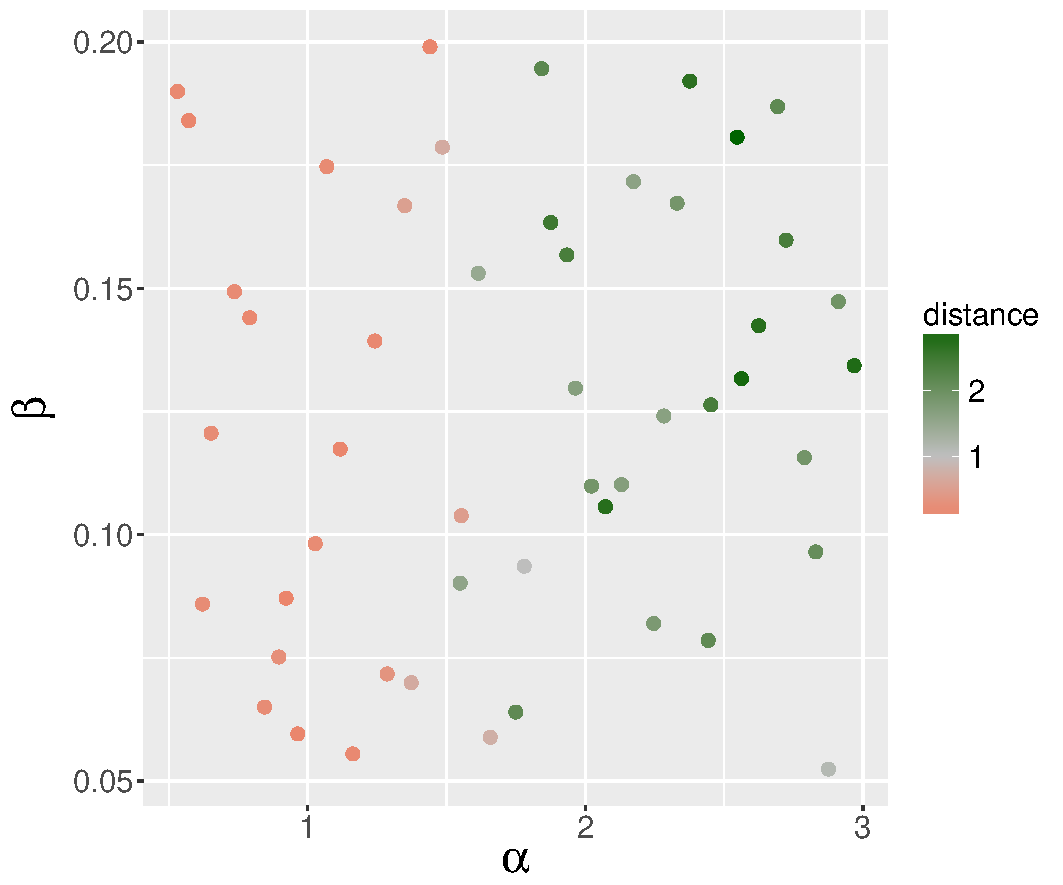
\includegraphics[width=0.49\linewidth]{Figures/Computation/relativedistance_metaparams}
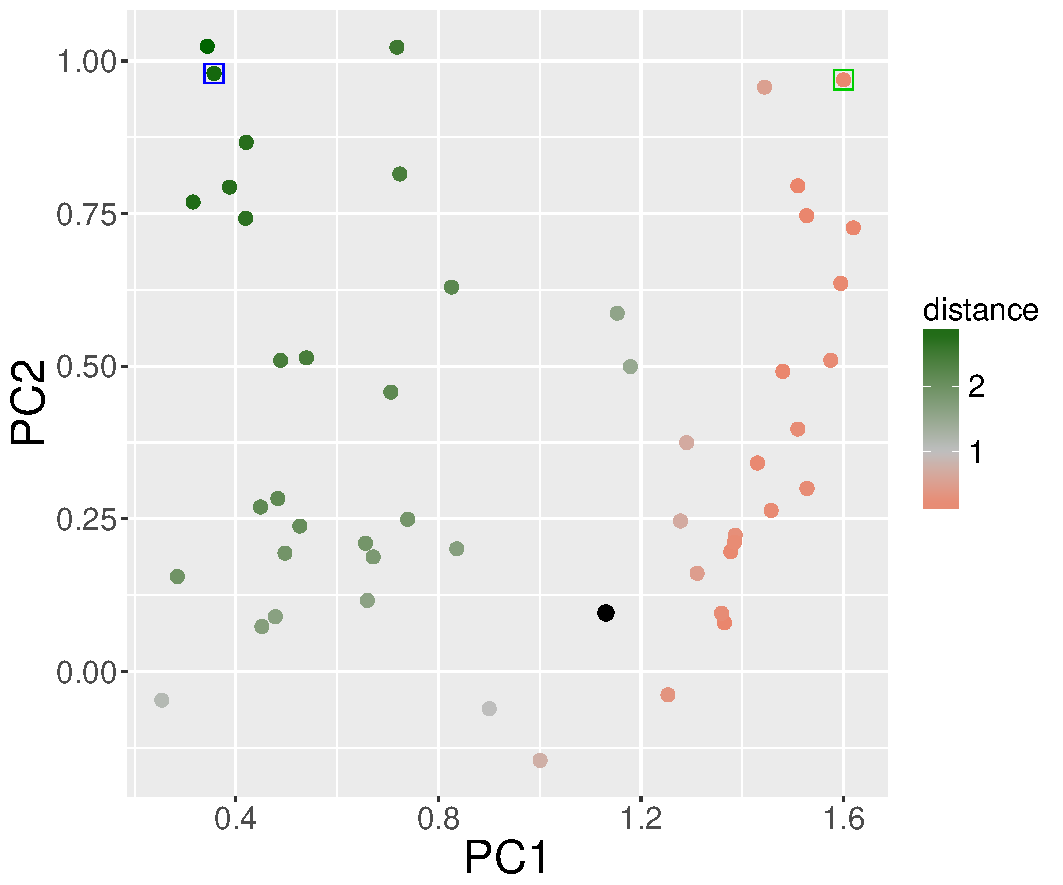
\includegraphics[width=0.49\linewidth]{Figures/Computation/relativedistance_morphspace}
\caption[Relative distances of phase diagrams to the reference][Distance des diagramme de phase à la référence]{\textbf{Relative distances of phase diagrams to the reference across grids.} (Top) Relative distance as a function of meta-parameters $\alpha$ (strength of preferential attachment) and diffusion ($\beta$, strength of diffusion process). (Bottom) Relative distance as a function of two first principal components of the morphological space (see text). Red point correspond to the reference spatial configuration. Green frame and blue frame give respectively the first and second particular phase diagrams shown in Fig.~\ref{fig:computation:sugarscape-phasediagrams}.\label{fig:computation:sugarscape-distance}}{\textbf{Distance relative des diagrammes de phase à la référence pour l'ensemble des grilles.} (Gauche) Distance relative comme fonction des meta-paramètres $\alpha$ (force de l'attachement préférentiel) et la diffusion ($\beta$, force du processus de diffusion). (Droite) Distance relative comme fonction des deux composantes principales de l'espace morphologique (voir texte). Le point rouge correspond à la configuration spatiale de référence. Les cadres verts et bleu donnent respectivement le premier et le second diagrammes particuliers montrés à la Fig.~\ref{fig:computation:sugarscape-phasediagrams}.\label{fig:computation:sugarscape-distance}}
\end{figure}
%%%%%%%%%%%%%



% phase diagrams -> ok well different qualitatively
%          spAlpha spDiffsteps spDiffusion spGrowth spPopulation
% id=27 : 0.7913103    2.376837   0.1440293 157.4147 4852.746
% id=0 : 2.562398    3.753032   0.1316788 128.4632 4753.983
% maxSugar = 110


%%%%%%%%%%%%%
\begin{figure}
\centering
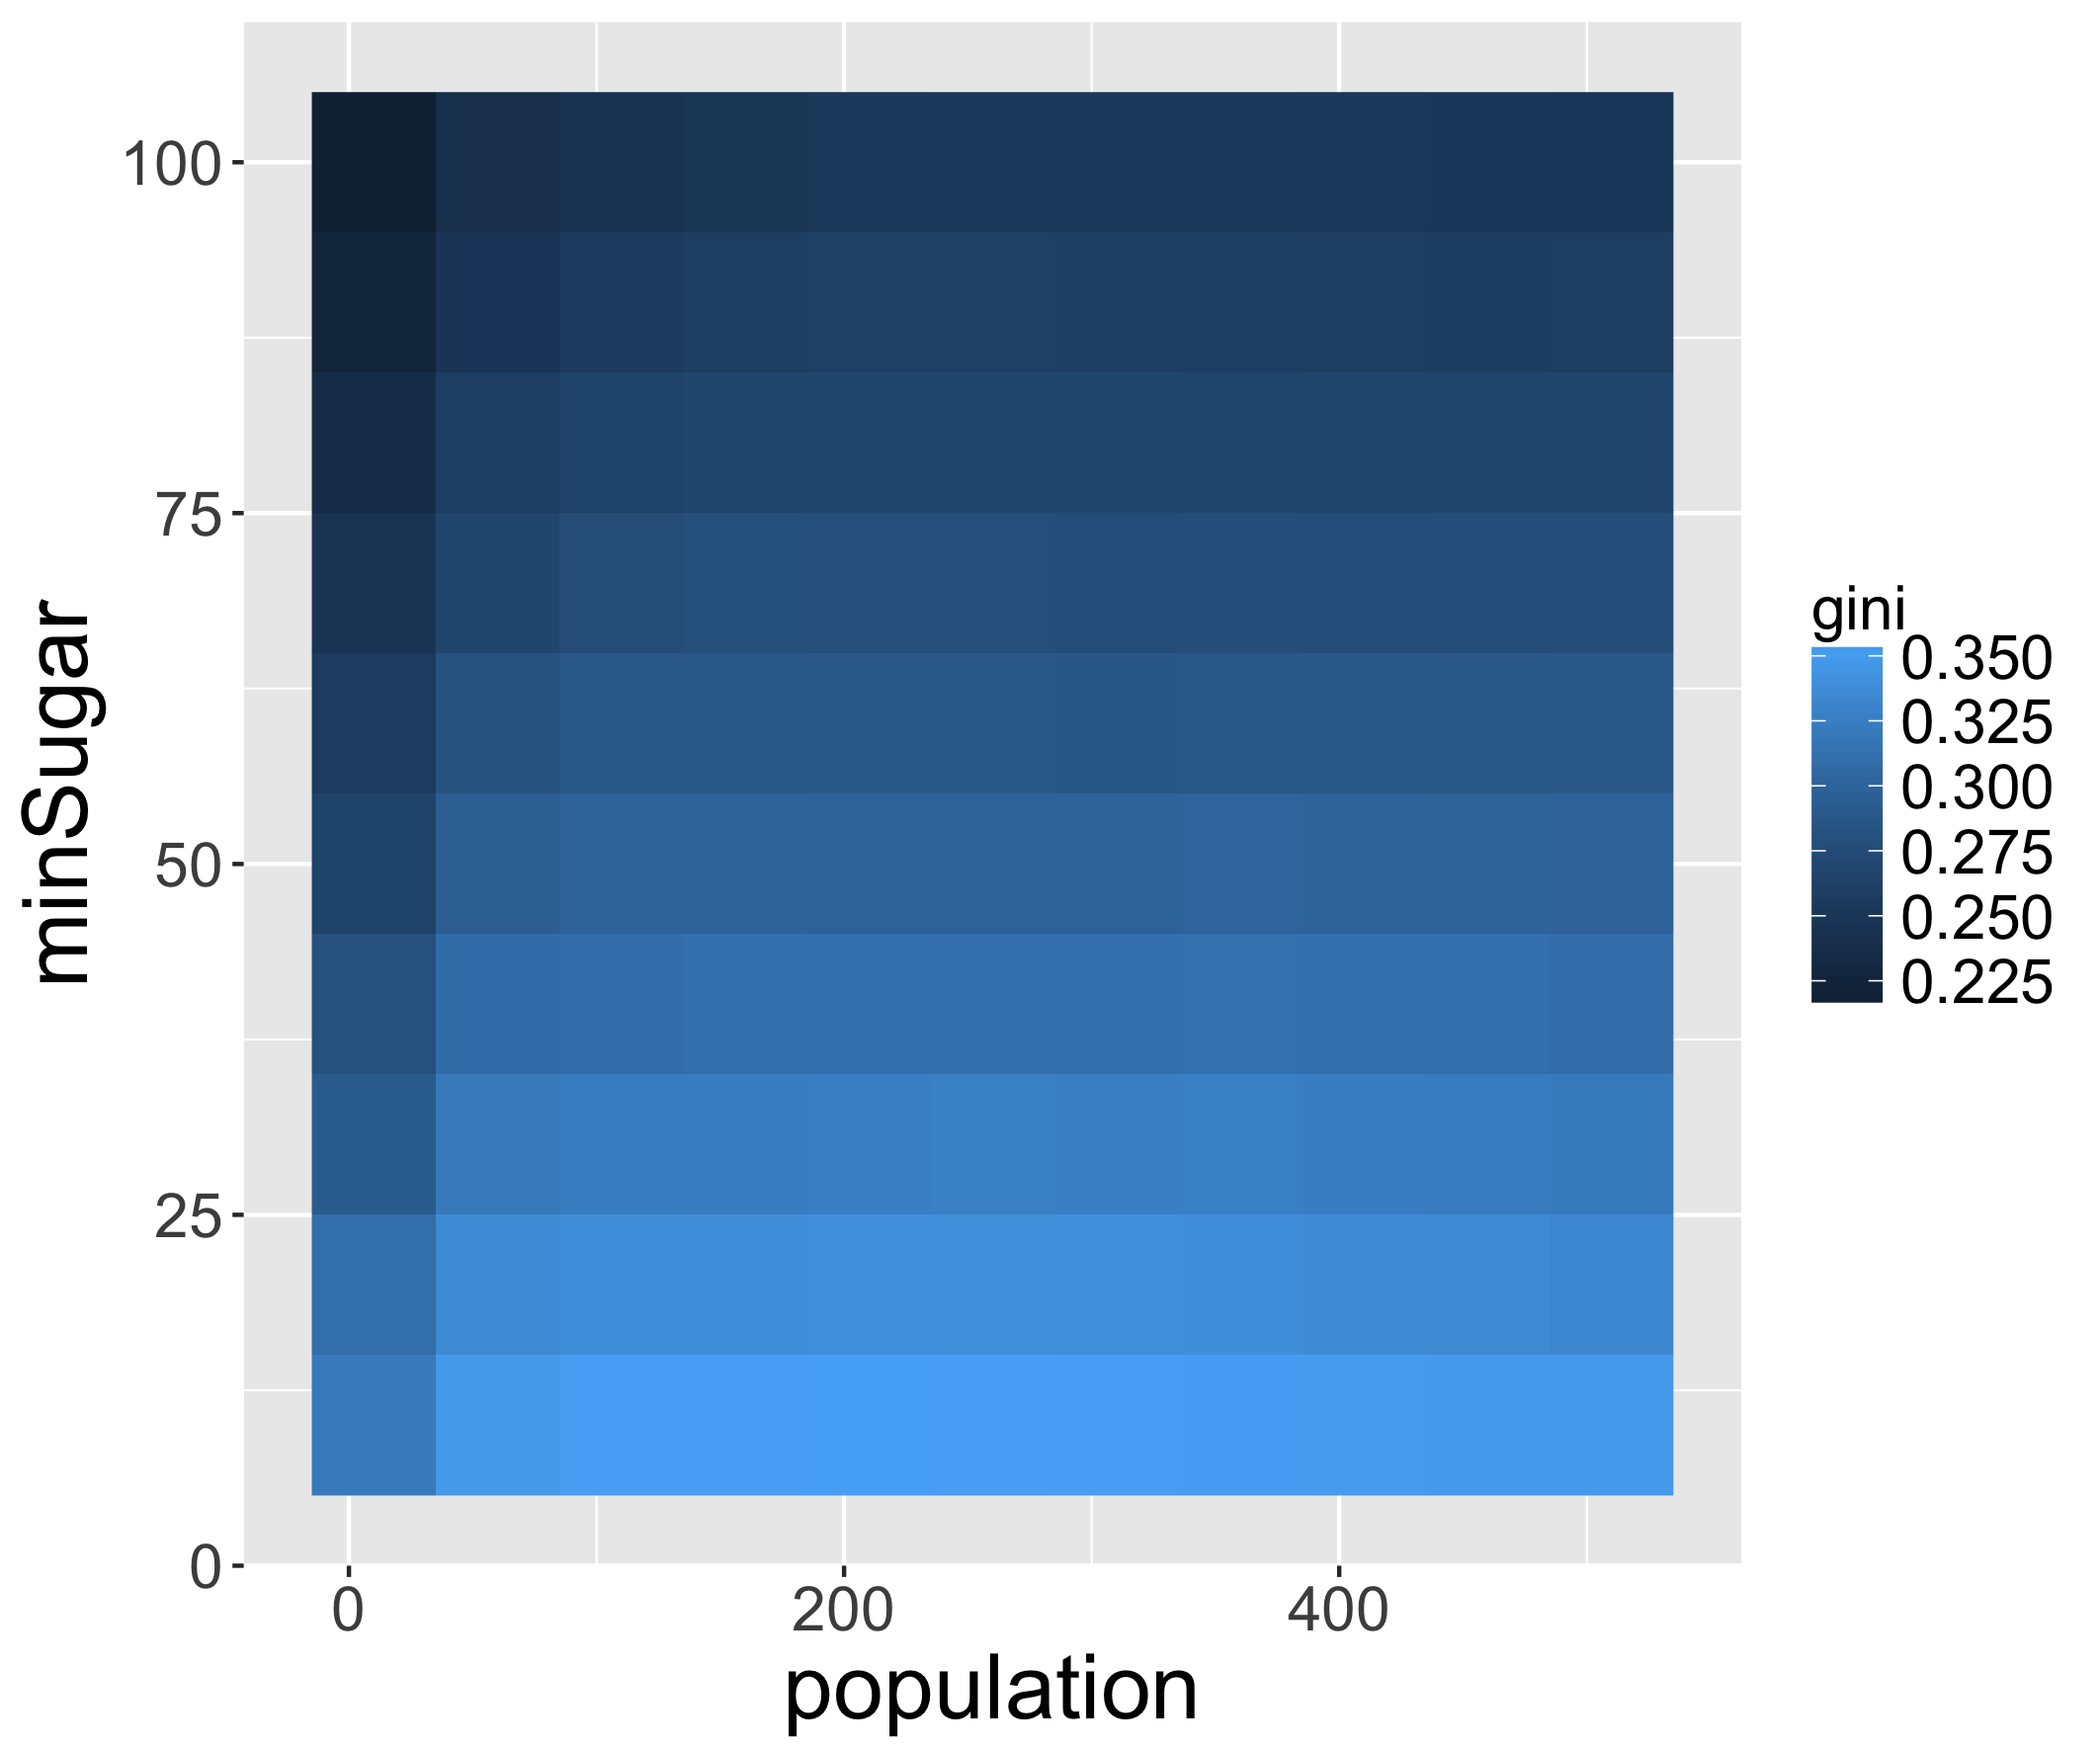
\includegraphics[width=0.49\linewidth]{Figures/Computation/phasediagram_id27_maxSugar110}
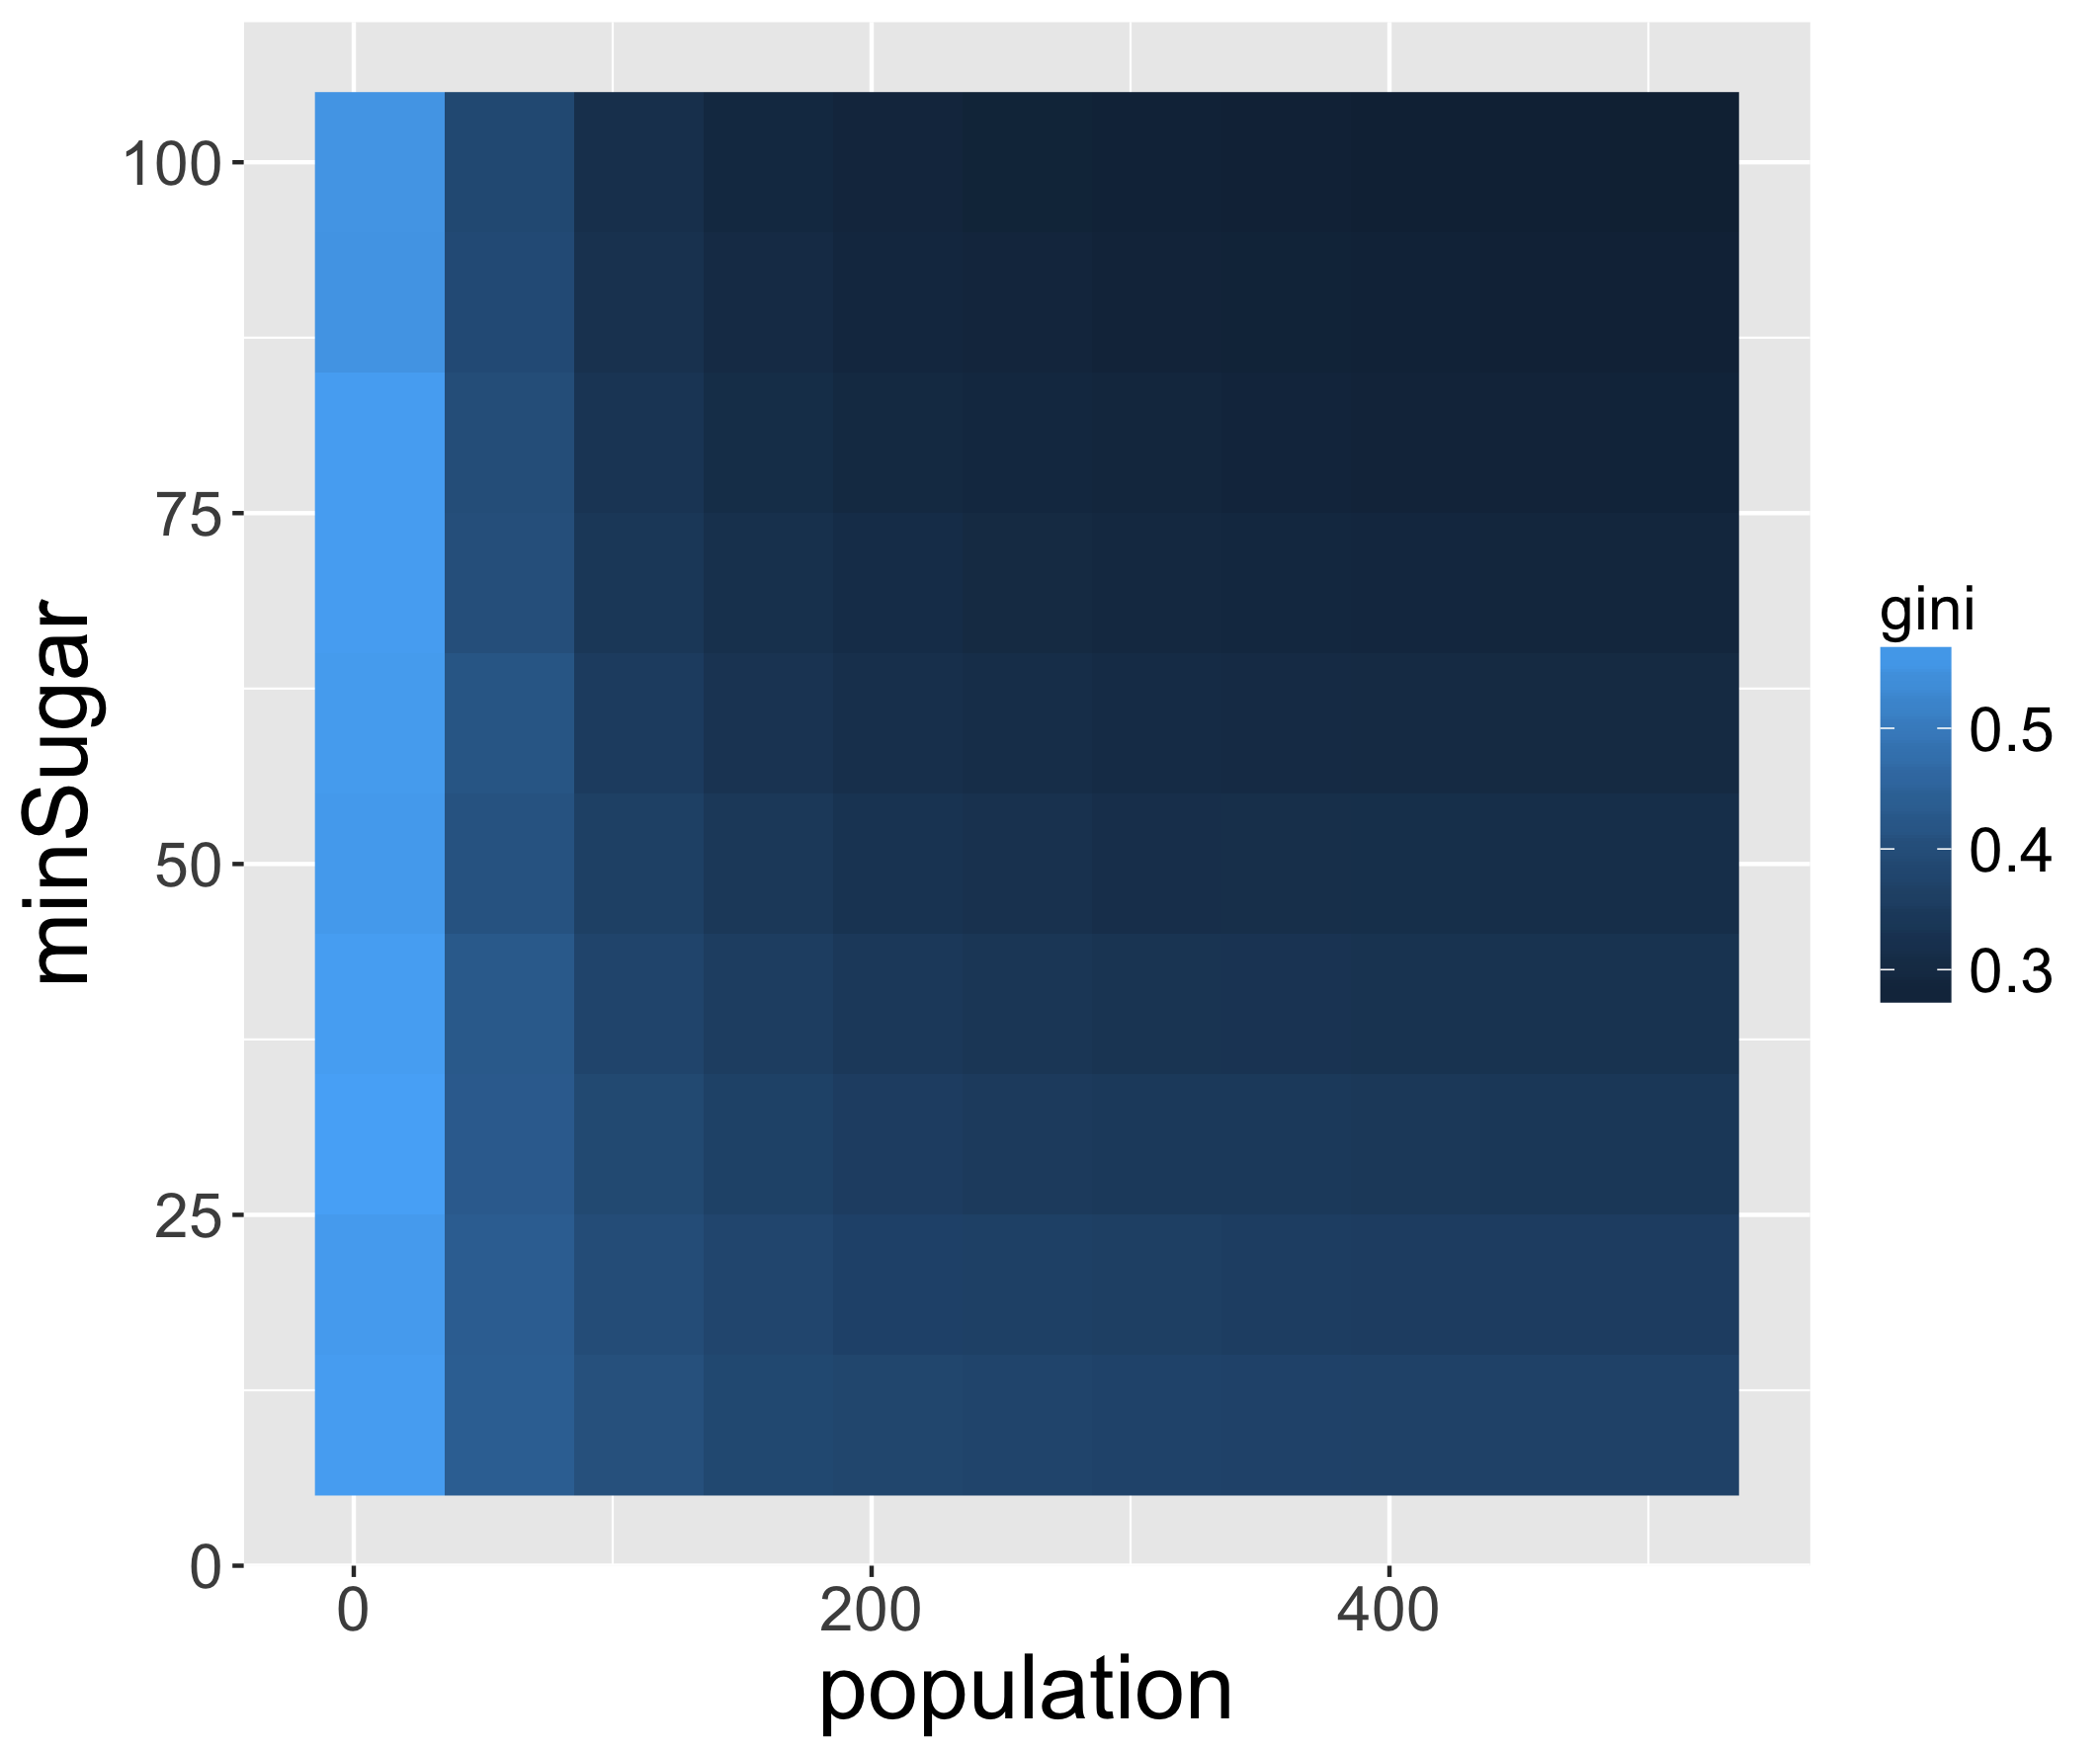
\includegraphics[width=0.49\linewidth]{Figures/Computation/phasediagram_id0_maxSugar110}
\caption[Examples of phase diagrams][Exemples de diagrammes de phase]{\textbf{Examples of phase diagrams.} We show two dimensional phase diagrams on $(P,s_-)$, both at fixed $s_+ = 110$. (Left) Green frame, obtained with $\alpha = 0.79$, $n=2$, $\beta = 0.14$, $N=157$; (Right) Blue frame, obtained with $\alpha = 2.56$, $n=3$, $\beta = 0.13$, $N=128$.\label{fig:computation:sugarscape-phasediagrams}}{\textbf{Exemples de diagrammes de phase.} Nous montrons deux diagrammes bi-dimensionnels sur $(P,s_-)$, obtenus à $s_+ = 110$ fixé. (Gauche) Cadre vert, obtenu avec $\alpha = 0.79$, $n=2$, $\beta = 0.14$, $N=157$ ; (Droite) Cadre bleu, obtenu avec $\alpha = 2.56$, $n=3$, $\beta = 0.13$, $N=128$.\label{fig:computation:sugarscape-phasediagrams}}
\end{figure}
%%%%%%%%%%%%%


\bpar{
We now check the sensitivity in terms of qualitative behavior of phase diagrams. We show the phase diagrams for two very opposite morphologies in term of sprawling, but controlling for aggregation with the same $PC2$ value. These correspond to the green and blue frames in Fig.~\ref{fig:computation:sugarscape-distance}. The behaviors are rather stable for varying $s_+$, what means that the poorest agents have a determinant role in trajectories. The two examples have not only a very distant baseline inequality (the ceil of the first 0.35 is roughly the floor of the second 0.3), but their qualitative behavior is also radically opposite: the sprawled configuration gives inequalities decreasing as population decreases and decreasing as minimal wealth increases, whereas the concentrated one gives inequalities strongly increasing as population decreases and also decreasing with minimal wealth but significantly only for large population values. The process is thus completely inverted, what would have significant impacts if one tried to schematize policies from this model. This second example confirms thus the importance of sensitivity of simulation models to the initial spatial conditions.
}{
Nous contrôlons à présent la sensibilité en terme de comportement qualitatif des diagrammes de phase. Nous montrons en Fig.~\ref{fig:computation:sugarscape-phasediagrams} les diagrammes pour deux morphologies très opposées en terme d'étalement, mais en contrôlant l'agrégation par la même valeur de $PC2$. Ceux-ci correspondent au cadres vert et bleu en Fig.~\ref{fig:computation:sugarscape-distance}. Les comportements sont relativement stables pour $s_+$ variant, ce qui signifie que les agents les plus pauvres ont un rôle déterminant dans les trajectoires. Les deux examples ont non seulement une inégalité de base très distance (le plafond du premier 0.35 est environ le plancher du second 0.3), mais leur comportement qualitatif est également radicalement opposé: la configuration étalée donne des inégalité qui décroissent quand la population décroît et qui décroissent quand la richesse minimale augmente, tandis que la concentrée donne des inégalités augmentant fortement quand la population décroît et aussi décroissantes avec la richesse minimale mais significativement seulement pour des grandes valeurs de population. Le processus est ainsi complètement inversé, ce qui aurait un impact déterminant si l'on essayait de schématiser des politiques à partir du modèle. Cet exemple confirme ainsi l'importance de la sensibilité des modèles de simulation aux conditions spatiales initiales.
}











\stars










%
% 3.3 Epistemological positioning



%----------------------------------------------------------------------------------------


\newpage



\section{Epistemological positioning}{Positionnement épistémologique}\label{sec:epistemology}

%----------------------------------------------------------------------------------------


\bpar{
The last section of this chapter aims at clarifying our epistemological positioning, since it has only been sketched at different points previously. Such a positioning is never harmless, since it strongly conditions the approaches, experiments and the interpretation of results: as \cite{morin1980methode} recalls, a positioning that pretends to be objective by rejecting any subjective component is much more biased than a conscious subjective approach.
}{
La dernière section de ce chapitre vise à clarifier notre positionnement épistémologique, celui-ci ayant déjà été ébauché à plusieurs occasions précédemment. Un tel positionnement n'est jamais anodin, puisqu'il conditionne fortement les démarches, les expériences et l'interprétation des résultats : comme le souligne~\cite{morin1980methode}, un positionnement qui se dit objectif en rejetant toute subjectivité est bien plus biaisé qu'une approche subjective consciente.
}


\bpar{
The points we wish to develop can be put into both a vertical perspective in terms of levels of abstraction and in a perspective of scientific domains: linearly, we first give the general epistemological context (typical to history of science, at a medium abstraction level), then switch at a less generic level to conceptually precise our particular objects (epistemology of the living and of the social), and finally take a broader perspective at the level of knowledge production itself (epistemology of complexity).
}{
Les points que nous souhaitons développer se placent dans une logique à la fois verticale de niveau d'abstraction et dans une logique de domaines scientifiques : dans l'ordre, nous posons d'abord le contexte épistémologique général (propre à l'histoire des sciences, à un niveau d'abstraction moyen), pour descendre en généralité et préciser conceptuellement nos objets particuliers (épistémologie du vivant et du social), pour finalement tout remettre en perspective au niveau de la production de connaissance elle-même (épistémologie de la complexité).
}



%%%%%%%%%%%%%%%%%%%%%%
\subsection{Cognitive approach and perspectivism}{Approche cognitive et perspectivisme}



\bpar{
Our epistemological positioning relies on a cognitive approach to science, given by Giere in~\cite{giere2010explaining}. The approach focuses on the role of cognitive agents as carriers and producers of knowledge. It has been shown to be operational by \cite{giere2010agent} that studies an agent-based model of science. These ideas converge with \noun{Chavalarias}' Nobel Game~\cite{chavalarias2016s} which tests through a stylized model the balance between exploration and falsification in the collective scientific enterprise.
}{
Notre positionnement épistémologique se fonde sur une approche cognitive de la science, introduite par \noun{Giere} dans~\cite{giere2010explaining}. L'approche se concentre sur le rôle des agents cognitifs comme porteurs et producteurs de la connaissance. Son caractère opérationnel a été montré par \cite{giere2010agent} qui étudie un modèle multi-agents de la science. Ces idées convergent avec le jeu Nobel de \noun{Chavalarias}~\cite{chavalarias2016s} qui teste de manière stylisée l'équilibre entre production de nouvelles théories et tentative de falsification de théories existantes dans l'entreprise scientifique collective.
}




\bpar{
This epistemological positioning has been presented by \noun{Giere} as \emph{scientific perspectivism}~\cite{giere2010scientific}, which main feature is to consider any scientific entreprise as a \emph{perspective} in which \emph{agents} use \emph{media} (models) to represent something with a certain purpose. To make it more concrete, we can position it within Hacking's ``check-list'' of constructivism~\cite{hacking1999social}, a practical tool to position an epistemological position within a simplified three dimensional space which dimensions are different aspects on which realist approaches and constructivist approach generally diverge: first the contingency (path-dependency of the knowledge construction process) is necessary in the pluralist perspectivist approach which assumes parallel paths of knowledge construction. Secondly the ``degree of constructivism'' is quite high because agents produce knowledge. Finally, concerning the endogenous or exogenous explanation of the stability of theories, this stability depends on the complex interaction between the agents and their perspectives, and is thus strongly endogenous, close to the positioning of constructivism. It was presented for these reasons as an intermediate and alternative way between absolute realism and skeptical constructivism~\cite{brown2009models}. The concept of \emph{perspective} will play thus a central role in the framework developed in~\ref{sec:knowledgeframework}.

}{
Ce positionnement épistémologique a été présenté par \noun{Giere} comme \emph{perspectivisme scientifique}~\cite{giere2010scientific}, dont la caractéristique principale est de considérer toute entreprise scientifique comme une \emph{perspective} dans laquelle des \emph{agents} utilisent des \emph{media} (modèles) pour représenter quelque chose dans un certain but. Pour comprendre ses principes de manière plus concrète, nous pouvons le positionner sur la \emph{check-list} du constructivisme de \noun{Hacking}~\cite{hacking1999social}, un outil pratique pour situer une position épistémologique. Celle-ci suppose un espace simplifié tri-dimensionnel dans lequel les dimensions sont différents aspects sur lesquels les approches réalistes et constructivistes généralement divergent. Le premier point est le niveau de contingence (dépendance au chemin du processus de construction de connaissances) : celle-ci est nécessaire dans l'approche perspectiviste qui est pluraliste et suppose des chemins parallèles de construction de connaissance. Le deuxième point mesure un ``degré de constructivisme'', qui est assez haut en perspectivisme car les agents produisent la connaissance. Enfin, le dernier point qui concerne l'explication endogène ou exogène de la stabilité des théories, est fortement du côté du constructivisme, puisque cette stabilité dépend des interactions complexes entre les agents et leur perspectives et donc totalement endogène. Le perspectivisme a pour ces raisons été présenté comme un chemin intermédiaire et alternatif entre le réalisme absolu et le constructivisme sceptique~\cite{brown2009models}. Le concept de \emph{perspective} jouera pour nous un rôle fondamental dans le cadre développé en~\ref{sec:knowledgeframework}.
}


\bpar{
Since this approach puts the emphasis on auto-organization, we consider it to be fully compatible with an anarchist view of science as advocated by~\cite{feyerabend1993against}. He formulates doubts on the relevance of political anarchism but introduces \emph{scientific anarchism}, which must not be understood as a full refusal of any ``objective'' method, but of an artificial authority and legitimacy that some scientific methods or currents would like to impose. He demonstrates through a precise analysis of Galileo's work that most of his results were based on beliefs and that most were not accessible with the current tools and methods at that time, and postulates that a similar logic should apply to contemporary works. There is thus no \emph{perspective} that is objectively more legitimate than others as soon as they are evidence-based and peer review validated - and even in this case legitimacy should be questionable, since questioning is one foundation of knowledge. It corresponds exactly to the plurality of perspectives we defend.
}{
Cette approche mettant l'emphase sur l'auto-organisation, nous la voyons totalement compatible avec une vision anarchiste de la science comme défendue par~\cite{feyerabend1993against}. Celui-ci émet des doutes sur l'intérêt de l'anarchisme politique mais introduit l'\emph{anarchisme scientifique}, qu'il ne faut pas comprendre comme un refus total de toute méthode ``objective'', mais d'une autorité et légitimité artificielle que certaines méthodes ou courants scientifiques pourraient vouloir prendre. Il démontre par une analyse précise des travaux de Galilée que la plupart de ses résultats étaient basés sur des croyances et que la plupart n'étaient pas accessibles avec les outils et méthodes de l'époque, et postule qu'il devrait en être de même pour certains travaux contemporains. Il n'y a donc pas de \emph{perspective} objectivement plus légitime que d'autres dans la mesure de leurs validation par des faits et des pairs - et même dans ces cas la légitimité doit pouvoir être discutée, car la remise en question est un fondement de la connaissance. Cela correspond exactement à la pluralité des perspectives que nous défendons.
}


\bpar{
Assuming an auto-organization and emergence of knowledge can be interpreted as a priority given to the \emph{bottom-up} construction of paradigms, trying to take some distance with preconceptions or dogmas that impose a top-down view. In other words, it is similar to practicing the scientific anarchism proposed by \noun{Feyerabend}. Indeed, anarchist positioning have found a very relevant echo in the different currents of complexity, from cybernetics to self-organization during the 20th century~\cite{duda2013cybernetics}. Our knowledge framework developed in~\ref{sec:knowledgeframework} illustrates this emergence of knowledge. Moreover, our will for reflexivity and to give to this work diverse reading paths beyond linearity (see Appendix~\ref{app:reflexivity}), shows the application of these principles. Methodological recommendations and positioning given previously in this chapter could sound as totalitarian if they were given roughly out of context, but these are indeed exactly the contrary since they sprout from a recent dynamic of open science which is well bottom-up founded, and in part a consequence of opening and plurality.
}{
Supposer auto-organisation et émergence des connaissances peut être interprété comme une priorité donnée à la construction des paradigmes \emph{par le bas} (\emph{bottom-up}), en tentant de se distancer des préconceptions ou dogmes cadrant par le haut. En d'autres termes, il s'agit de pratiquer l'anarchisme scientifique prôné par \noun{Feyerabend}. En effet, les positions anarchistes ont trouvé un écho très cohérent dans les différents courants de la complexité, de la cybernétique à l'auto-organisation au cours du 20ème siècle~\cite{duda2013cybernetics}. Notre cadre de connaissances développé en~\ref{sec:knowledgeframework} illustre cette émergence de la connaissance. De plus, notre volonté de réflexivité et de donner à notre travail des pistes de lecture diverses au delà de la linéarité (voir Annexe~\ref{app:reflexivity}), montre l'application de ces principes. Les recommandations méthodologiques et les positionnements donnés précédemment dans ce chapitre pourraient sonner comme totalitaires s'ils étaient assénés de manière sèche sans contexte, mais ceux-ci sont en fait tout le contraire puisqu'ils découlent d'une dynamique récente de science ouverte qui a bien émergé par le bas, conséquence en partie de l'ouverture et de la pluralité.
}

% Concept of ``Deconstructivism'' ? does not seen to exist.






%%%%%%%%%%%%%%%%%%%%%%
\subsection{From life to culture}{De la Vie à la Culture}

\subsubsection{Biological systems and social systems}{Systèmes biologiques et systèmes sociaux}


\bpar{
The parallel between social and biological systems is not rare, sometimes more from an analogy perspective as for example in \noun{West}'s \emph{Scaling} theory which applies similar growth equations starting from scaling laws, with however inverse conclusions concerning the relation between size and pace of life~\cite{bettencourt2007growth}. Scaling relations do not hold when we try to apply them to a single ant, and they must be applied to the whole ant colony which is then the organism studied. When adding the property of cognition, we confirm that it is the relevant level, since the colony shows advanced cognitive properties, such as the resolution of spatial optimization problems, or the quick answer to an external perturbation. Human social organizations, cities, could be seen as organisms ? \cite{banos2013pour} extends the metaphor of the \emph{urban anthill} but recalls that the parallel stops quickly. We will however see to what extent some concepts from the epistemology of biology can be useful to understand social systems that we propose to study.
}{
Le parallèle entre les systèmes sociaux et les systèmes biologiques est souvent fait, parfois de manière plus qu'imagée comme par exemple pour la théorie du \emph{Scaling} de \noun{West} qui applique des équations de croissance similaires à partir des lois d'échelle, avec des conclusions inverses tout de même concernant la relation entre taille et rythme de vie~\cite{bettencourt2007growth}. Les relations d'échelle ne tiennent plus lorsqu'on essaye de les appliquer à une fourmi seule, et il faut alors l'appliquer à la fourmilière entière qui est l'organisme en question. En ajoutant la propriété de cognition, on confirme qu'il s'agit du niveau pertinent, puisque celle-ci possède des propriétés cognitives avancées, comme la résolution de problèmes d'optimisation spatiaux, ou la réponse rapide à une perturbation extérieure. Les organisations sociales humaines, les villes, peuvent-elles être vues comme des organismes ? \cite{banos2013pour} file la métaphore de la \emph{fourmilière urbaine} mais rappelle que le parallèle s'arrête assez vite. Nous allons voir cependant dans quelle mesure certains concepts de l'épistémologie de la biologie peuvent être utiles pour comprendre les systèmes sociaux que nous nous proposons d'étudier.
}


\bpar{
We start from the fundamental contribution of \noun{Monod} in~\cite{monod1970hasard}, which aims at developing crucial epistemological principles for the study of life. Thus, living organisms answer to three essential properties that differentiate them from other systems: (i) the teleonomy , i.e. the property that these are ``objects with a project'', project that is reflected in their structure and the structure of artifacts they produce\footnote{That must not be mistaken with teleology, typical of animist thoughts, that consists in giving a project or a meaning to the universe.}; (ii) the importance of morphogenetic processes in their constitution (see~\ref{sec:interdiscmorphogenesis}); (iii) the property of the invariant reproduction of information defining their structure. \noun{Monod} furthermore sketches in conclusion some paths towards a theory of cultural evolution. Teleonomy is crucial in social structures, since any organization aims at satisfying a set of objectives, even if in general it will not succeed and the objectives will co-evolve with the organization. This notion of multi-objective optimization is typical of complex socio-technical systems, and will be more crucial than for biological systems.
}{
Nous nous basons sur la contribution fondamentale de \noun{Monod} dans~\cite{monod1970hasard}, qui tente de développer les principes épistémologiques cruciaux pour l'étude du vivant. Ainsi, les organismes vivants répondent à trois propriétés essentielles qui permettent des les différencier d'autres systèmes : (i) la téléonomie, c'est-à-dire qu'il s'agit ``d'objets doués d'un projet'', projet qui se reflète dans leur structure et dans celles des artefacts qu'ils produisent\footnote{Qu'il ne faut pas confondre avec la téléologie, propres aux animismes, qui consiste à prêter un projet ou un sens à l'univers.} ; (ii) l'importance des processus morphogénétiques dans leur constitution (voir~\ref{sec:interdiscmorphogenesis}) ; (iii) la propriété de reproduction invariante de l'information définissant leur structure. \noun{Monod} esquisse de plus en conclusion des pistes pour une théorie de l'évolution culturelle. La téléonomie est essentielle dans les structures sociales, puisque toute organisation essaye de satisfaire un ensemble d'objectifs, même si en général elle n'y parviendra pas et que ceux-ci co-évolueront avec l'organisation. Cette notion d'optimisation multi-objectif est typique des systèmes complexes socio-techniques, et y sera plus cruciale que pour les systèmes biologiques.
}


\bpar{
Moreover, we postulate that the concept of morphogenesis is an essential tool to understand these systems, with a definition very similar to the one used in biology. A more thorough work to build this definition is done in~\ref{sec:interdiscmorphogenesis}, that we will sum up as the existence of relatively autonomous processes guiding the growth of the system and implying causal circular relations between form and function, that witness an emergent architecture. For social systems, isolating the system is more difficult and the notion of boundary will be less struct than for a biological system, but we will indeed find this link between form and function, such as for example the structure of an organization that impacts its functionalities.
}{
Ensuite, nous postulons que le concept de morphogenèse est un outil essentiel pour comprendre ces systèmes, avec une définition très proche de celle utilisée en biologie. Un travail approfondi pour donner cette définition est fait en~\ref{sec:interdiscmorphogenesis}, que nous résumerons en l'existence de processus relativement autonomes guidant la croissance du système et impliquant des relations causales circulaires entre forme et fonction qui témoignent d'une architecture émergente. Pour des systèmes sociaux, isoler le système est plus difficile et la notion de frontière sera moins stricte que pour un système biologique, mais on retrouvera bien ce lien entre forme et fonction, comme par exemple la structure d'une organisation ayant un impact sur ses fonctionnalités.
}


\bpar{
Finally, the reproduction of information is at the core of cultural evolution, through the transmission of culture and \emph{memetics}, the difference being that the ratio of scales between the frequency of transmission and mutation and cross-over processes or other non-memetic processes of cultural production is relatively low, whereas is many orders of magnitude in biology.
}{
Enfin, la reproduction de l'information est au coeur de l'évolution culturelle, par la transmission de la culture et la \emph{mémétique}, la différence étant que le rapport d'échelles de temps entre la fréquence de transmission et les processus de croisement et de mutation ou d'autres processus non mémétiques de production culturelle est relativement faible, alors qu'elle est de plusieurs ordres de grandeur en biologie.
}


\bpar{
An example shows that the parallel is not always absurd : \cite{2017arXiv170305917G} proposes an auto-catalytic network model for cognition, that would explain the apparition of cultural evolution through processes that are analogous to the ones that occurred at the apparition of life, i.e. a transition allowing the molecules to be self-sustained and to self-reproduce, mental representations being the analogous of molecules.
}{
Un exemple illustre que le parallèle n'est pas toujours absurde : \cite{2017arXiv170305917G} propose un modèle de réseau auto-catalytique pour la cognition, qui expliquerait l'apparition de l'évolution culturelle par des processus analogues à ceux s'étant produit à l'apparition de la vie, c'est-à-dire une transition permettant au molécules de s'auto-entretenir et s'auto-reproduire, les représentations mentales faisant office de molécules.
}


\bpar{
But even if processes are at the origin analogous, the nature of evolution is then quite different, as show \cite{vanderLeeuw2009}, darwinian criteria for evolution being not sufficient to explain the evolution of our organized societies. This is a complexity of a different nature in which the role of information flows is crucial (see the role of informational complexity in the next subsection).
}{
Mais si les processus à l'origine sont analogues, la nature de l'évolution est bien différente par la suite, comme le montrent \cite{vanderLeeuw2009}, les critères darwiniens d'évolution n'étant pas suffisant pour expliquer l'évolution de nos sociétés organisées. Il s'agit d'une complexité de nature différente dans laquelle le rôle des flux d'information est crucial (voir le rôle de la complexité informationnelle dans la sous-section suivante). 
}


\bpar{
One point that also must retain our attention is the greater difficulty to define levels of emergence for social systems: \cite{roth2009reconstruction} underlines the risk to fall into ontological dead-ends if levels were badly defined. He argues that more generally we must go past the single dichotomy micro-macro that is used as a caricature of the concepts of weak emergence, and that ontologies must often be multi-level and imply multiple intermediate levels.
}{
L'un des points sur lequel il s'agit également d'être attentif est la plus grande difficulté de définir les niveaux d'émergence pour les systèmes sociaux : \cite{roth2009reconstruction} souligne le risque de tomber dans des cul-de-sac ontologiques car les niveaux ont été mal définis. Il soutient qu'il faut d'une manière générale penser au-delà de la seule dichotomie micro-macro qui est utilisée pour caricaturer les concepts d'émergence faible, et que les ontologies doivent souvent être multi-niveaux et impliquant de multiples niveaux intermédiaires.
}


\bpar{
This last question must also be put into perspective with the problem of the existence of strong emergence in social structures, that in sociological terms corresponds to the idea of the existence of ``collective beings''~\cite{angeletti2015etres}. \noun{Morin} indeed distinguishes living systems of the second type (multi-cellular) and of the third type (social structures), but precises that the \emph{subjects} of the latest are necessarily unachieved\cite{morin1980methode} (p.~852). Thus, emergences from the biological to the social are analogous by stay fundamentally different.
}{
Cette dernière question est aussi à mettre en perspective avec le problème de l'existence d'émergence forte dans les structures sociales, qui en termes sociologiques correspond à l'idée de l'existence ``d'êtres collectifs''~\cite{angeletti2015etres}. \noun{Morin} distingue d'ailleurs les systèmes vivants du second type (multi-cellulaire) et du troisième type (structures sociales), mais précise que les \emph{sujets} de ces derniers sont nécessairement inachevés~\cite{morin1980methode} (p.~852). Ainsi, les émergences du biologique au social sont analogues mais restent fondamentalement différentes.
}



\subsubsection{Co-evolution}{Co-évolution}



\bpar{
This positioning on biological and social systems finds a direct echo for the concept of co-evolution. It indeed comes from biology, where it was developed following the concept of evolution, to be used more recently in social sciences and humanities. To what extent the concept was transfered ? Is there a parallel similar to the one between biological evolution and cultural evolution ? We propose, in order to answer these questions, to develop a brief multidisciplinary point of view on co-evolution\footnote{The approach here is slightly different from the one lead in~\ref{sec:interdiscmorphogenesis} in the case of morphogenesis, that will be \emph{interdisciplinary} in the sens that it aims at integrating approaches, whereas we stay here in an overview of concepts and thus more in a \emph{multidisciplinary} approach. The concept of \emph{co-evolution} being key for our empirical work in the following, we will therefore give an original characterization to it, and make the choice to not go into an integrative syncretism for this concept, but indeed to approach it from a \emph{geographical point of view}, and even more precisely in the frame of territorial systems. We could postulate a congruence between the empirical and modeling specialization and the one for theory, reading our process of knowledge production in a particular profile of knowledge domains dynamics (see~\ref{sec:knowledgeframework}).}. We will in the following review a broad spectrum of disciplines, starting from biology where the concept originated to progressively come to disciplines closer to territorial sciences.
}{
Ce positionnement sur les systèmes biologiques et sociaux trouve un écho immédiat pour le concept de co-évolution. Il provient en effet de la biologie, où il a été développé à la suite de celui d'évolution, pour être utilisé plus récemment en sciences humaines et sociales. Dans quelle mesure le concept a-t-il été transféré ? Retrouve-t-on un parallèle similaire à celui entre évolution biologique et évolution culturelle ? Nous proposons pour répondre à ces questions d'apporter un bref point de vue multidisciplinaire sur la co-évolution\footnote{La démarche ici est légèrement différente de celle que nous mènerons en~\ref{sec:interdiscmorphogenesis} dans le cas de la morphogenèse, qui sera \emph{interdisciplinaire} au sens où elle cherchera à intégrer les approches, tandis que nous restons ici dans un aperçu des concepts et donc plutôt dans du \emph{multidisciplinaire}. Le concept de \emph{co-évolution} étant clé pour notre travail empirique par la suite, nous en donnerons alors une caractérisation originale et prenons le parti de ne pas tomber dans le syncrétisme intégrateur pour ce concept, mais bien de l'approcher d'un \emph{point de vue géographique}, et même plus précisément dans le cadre des systèmes territoriaux. On pourrait postuler une congruence entre la spécialisation empirique/de modélisation et celle théorique, plaçant notre processus de production de connaissance dans un profil particulier de dynamiques de domaines de connaissance (voir~\ref{sec:knowledgeframework}).}. Nous passons par la suite en revue un large spectre de disciplines, partant de la biologie où le concept a initialement trouvé son origine pour arriver progressivement à des disciplines en relation avec les sciences du territoire.
}



\subsubsection{Biology}{Biologie}

\bpar{
The concept of co-evolution in biology is an extension of the well-known concept of \emph{evolution}, that can be tracked back to \noun{Darwin}. \cite{durham1991coevolution} (p.~22) recalls the components and systemic structures that are necessary to have evolution\footnote{And in that general context, evolution is not restricted to the biology of life and the presence of genes, but also to physical systems verifying these conditions. We will come back to that later.}.
}{
Le concept de co-évolution en biologie est une extension de celui bien connu d'\emph{évolution}, qui remonte à \noun{Darwin}. \cite{durham1991coevolution} (p.~22) rappelle les composantes et structure systémiques nécessaires pour qu'il y ait évolution\footnote{Et dans ce contexte général l'évolution n'est pas réservée à la biologie du vivant et la présence de gènes, mais aussi à des systèmes physiques vérifiant ces conditions. Nous y reviendrons plus loin.}.
}

\bpar{
\begin{enumerate}
\item Process of \emph{transmission}, implying transmission units and transmission mechanisms.
\item Process of \emph{transformation}, that necessitates sources of variation.
\item Isolation of sub-systems such that the effects of previous processes are observable in differentiations.
\end{enumerate}
}{
\begin{enumerate}
	\item Processus de \emph{transmission}, impliquant des unités de transmission et des mécanismes de transmission.
	\item Processus de \emph{transformation}, nécessitant des sources de variation.
	\item Isolation de sous-systèmes pour que les effets des processus précédents soient observables dans des différentiations.
\end{enumerate}
}

\bpar{
This way, a population submitted to constraints (often conceptually synthesized as a \emph{fitness}) that condition the transmission of the genetic heritage of individuals (transmission), and to random genetic mutations (transformation), will indeed be in evolution in the spatial territories it populates (isolation), and by extension the species to which it can be associated. 
}{
Ainsi, une population soumise à des contraintes (souvent synthétisées conceptuellement comme une \emph{fitness}) qui conditionnent la transmission du patrimoine génétique des individus (transmission), et à des mutation génétiques aléatoires (transformation), sera bien en évolution dans les territoires spatiaux qu'elle occupe (isolation), et par extension l'espèce à laquelle on peut l'associer.
}


La co-évolution est alors définie comme un changement évolutionnaire dans une caractéristique des individus d'une population, en réponse à un changement dans une deuxième population qui à son tour répond évolutionnairement au changement de la première, comme synthétisé par~\cite{janzen1980coevolution}. Cet auteur appuie par ailleurs la subtilité du concept et alerte contre ses utilisations injustifiées : la présence d'une congruence de deux caractéristiques qui semblent adaptées l'une à l'autre n'implique pas l'existence d'une co-évolution, l'une des deux espèces ayant pu s'adapter seule à une caractéristique déjà présente de l'autre.

Cette présentation brute de décoffrage mutile dans une certaine mesure la complexité réelle des écosystèmes : les populations s'insèrent dans des réseaux trophiques et des environnements, et les interactions co-évolutionnaires impliqueraient des communautés de populations d'espèces diverses, comme présenté par \cite{strauss2005toward} sous l'appellation de co-évolution diffuse. De même, les dynamiques spatio-temporelles sont cruciales dans la réalisation de ces processus : \cite{dybdahl1996geography} étudient par exemple l'influence de la distribution spatiale sur les motifs de co-évolution pour un escargot et son parasite, et montre qu'une vitesse de diffusion génétique dans l'espace plus grande pour le parasite conduit les dynamiques de co-évolution.

Les concepts essentiels à retenir du point de vue biologique sont ainsi : (i) existence de processus d'évolution, en particulier transmission et transformation ; (ii) dans des schémas circulaires entre populations dans le cas de la co-évolution ; et (iii) dans un cadre territorial (spatio-temporel et environnemental au sens du reste de l'éco-système) complexe.


\subsubsection{Cultural evolution}{Evolution culturelle}


Ce développement sur la co-évolution nous a été amené par le parallèle entre systèmes biologiques et systèmes sociaux. L'évolution de la culture est théorisée est explorée par un champ propre, et n'est pas en reste de dynamiques co-évolutives. \cite{Mesoudi25072017} rappelle l'état des connaissances sur le sujet et les défis à venir, comme la relation avec la nature cumulative de la culture, l'influence de la démographie dans les processus d'évolution, ou la construction de méthodes phylogénétiques permettant de reconstruire des arbres des branchements passés.

Pour donner un exemple, \cite{carrignon2015modelling} introduit un cadre conceptuel pour la co-évolution de la culture et du commerce dans le cas de sociétés anciennes sur lesquelles on dispose de données archéologiques, et propose son implémentation par un modèle multi-agents dont les dynamiques sont partiellement validées par l'étude des faits stylisés produits par le modèle. La co-évolution est bien prise ici au sens d'adaptation mutuelle de structures socio-spatiales, à des échelles de temps comparables, dans ce cadre plus général d'évolution culturelle.


L'évolution culturelle serait même indissociable de l'évolution génétique, puisque \cite{durham1991coevolution} postule et illustre un lien fort entre les deux, qui seraient eux-mêmes en co-évolution. \cite{bull2000meme} explore un modèle stylisé impliquant deux populations de répliquants (les gènes et les memes) et montre l'existence de transitions de phase pour les résultats du processus d'évolution génétique lorsque l'interaction avec le répliquant culturel est forte.


%\subsubsection{Artificial Life}{Artificial Life}
% -> in cultural evolution

\subsubsection{Sociology}{Sociologie}

Le concept a été utilisé en sociologie et disciplines apparentées comme les études de l'organisation, suivant le parallèle effectué ci-dessus de la même manière que pour l'évolution culturelle. Dans le domaine de l'étude des organisations, \cite{volberda2003co} développe un cadre conceptuel de la co-évolution inter-organisationnelle en relations avec les processus de management internes, mais déplore l'absence d'études empiriques cherchant à quantifier cette co-évolution. Dans le cadre de la gestion des systèmes de production, \cite{tolio2010species} conceptualise un chaine de production intelligente où produit, processus et système de production doivent être en co-évolution.


\subsubsection{Economic geography}{Economie géographique}


En économie géographique, le concept de co-évolution a également largement été mobilisée. L'idée d'entités évolutionnaires en économie vient à contre-courant du courant néoclassique qui reste majoritaire, mais trouve un écho de plus en plus pertinent~\cite{nelson2009evolutionary}. \cite{schamp201020} procède à une analyse épistémologique de l'utilisation de la co-évolution, et oppose une approche néo-schumpeterienne de l'économie qui considère l'émergence de populations qui évoluent à partir de règles micro-économiques (qui correspondrait à une lecture directe et relativement isolationniste de l'évolution biologique) à une approche systémique qui considérerait l'économie comme un système évolutif de manière globale (qui correspondrait à l'évolution diffuse que nous avons développé précédemment), pour proposer une caractérisation précise tombant dans le premier cas, qui suppose des \emph{institutions} qui co-évoluent. Le plus important pour notre propos est qu'il souligne l'aspect crucial du choix des population et des entités considérées, de la zone géographique, et appuie l'importance de l'existence de relations causales circulaires.

Il est possible de donner divers exemples d'application. \cite{doi:10.1080/00343400802662658} introduit un cadre conceptuel pour permettre de concilier nature évolutionnaire des entreprises, théorie des clusters et réseaux de connaissance, dans lequel la co-évolution entre réseaux et entreprises est centrale, et qui est définie comme une causalité circulaire entre différentes caractéristiques de ces sous-systèmes. \cite{colletis2010co} introduit un cadre de co-évolution des territoires et de la technologie (questionnant par exemple le rôle de la proximité pour les innovations), qui révèle l'importance à nouveau de l'aspect institutionnel. \cite{ter2011co} propose un cadre couplant la vision évolutionnaire des entreprises, la littérature sur les industries et l'innovation dans les clusters, et l'approche par réseau complexe des connexions entre ces premiers dans le système territorial.

En économie environnementale, \cite{kallis2007coevolution} montre que des approches ``larges'' (pouvant considérer la majorité des co-dynamiques comme co-évolutives) s'opposent à des approches plus strictes (dans l'esprit de la définition donnée par \cite{schamp201020}), et que dans tous les cas une définition précise, pas forcément venant de la biologie, doit être donnée, en particulier pour la recherche d'une caractérisation empirique.




\subsubsection{Geography}{Géographie}

Pour la géographie, comme nous l'avons déjà présenté en introduction, les travaux les plus proches empiriquement et théoriquement des notions de co-évolution sont étroitement liés à la théorie évolutive des villes. Il n'est pas évident de tracer dans la littérature à quel moment la notion a été clairement formalisée, mais il est évident qu'elle était présente dès les fondements de la théorie comme le rappelle \noun{Denise Pumain} (voir~\ref{app:sec:interviews}) : le système complexe adaptatif est composé de sous-systèmes en interdépendances complexes, souvent circulairement causales. Les premiers modèles incluent bien cette vision de manière implicite, mais la co-évolution n'est pas appuyée explicitement ou définie précisément, en termes qui seraient quantifiables ou identifiables structurellement. \cite{paulus2004coevolution} a amené des preuves empiriques de mécanismes de co-évolution par l'étude de l'évolution des profils économiques des villes françaises. L'interprétation utilisée par~\cite{schmitt2014modelisation} repose sur une entrée par la théorie évolutive des villes, et consiste fondamentalement en une lecture des systèmes de villes comme entités fortement interdépendantes.


\subsubsection{Physical Geography}{Géographie physique}

En étude des paysages, \cite{sheeren2015coevolution} parlent de co-évolution du paysage et des activités agricoles, mais ne considèrent en fait pas d'effet circulaires de l'un sur l'autre. A priori, leurs résultats montrent que l'évolution des pratiques agricoles entraine une évolution du paysage, et il n'est ainsi pas clair dans quelle mesure le cadre conceptuel de la co-évolution, mentionné sans plus de détails, est mobilisé.


\subsubsection{Physics}{Physique}

Enfin, on peut noter de manière anecdotique que le terme de co-évolution a également été utilisé par la physique. L'utilisation pour des systèmes physiques peut porter à débat, selon que l'on suppose ou non que la transmission suppose un transmission d'\emph{information}\footnote{L'information est définie dans la théorie shanonienne comme une probabilité d'occurrence d'une chaîne de caractère. \cite{morin1976methode} montre que le concept d'information est en fait bien plus complexe, et qu'il doit être pensé conjointement à un contexte donné de génération d'un système auto-organisateur néguentropique, i.e. réalisant des diminutions locales d'entropie notamment grâce à cette information. Ce type de système est nécessairement vivant. Nous prendrons ici cette vision complexe de l'information.}. Dans le cas d'une transmission ontologique uniquement physique (\emph{êtres physiques}), alors une grande partie des systèmes physiques sont évolutifs. \cite{hopkins2008cosmological} développe un cadre cosmologique pour la co-évolution d'objets cosmiques hétérogènes dont la présence et les dynamiques sont difficilement expliquées par des théories plus classiques (certains types de galaxies, quasars, trous noirs supermassifs). \cite{antonioni2017coevolution} étudie la co-évolution entre des propriétés de synchronisation et de coopération au sein d'un réseau d'oscillateurs de Kuramoto\footnote{Le modèle de Kuramoto s'intéresse à la synchronisation au sein de systèmes complexes, en étudiant l'évolution de phases $\theta_i$ couplée par les équations d'interaction $\dot{\vec{\theta}} = \vec{\omega} + \vec{W}\left[\vec{\theta}\right] + \mathbf{B}$ où $\vec{\omega}$ sont les phases propres de forçage et la force de couplage entre $i$ et $j$ est donnée par $\vec{W}_{i} = \sum_j w_{ij} \sin\left(\theta_i - \theta_j\right)$ et $\vec{B}$ du bruit.}, montrant d'une part que le concept peut être appliqué à des objets abstraits, et d'autre part qu'un réseau de relations complexes entre variables peut être à l'origine de dynamiques présentant des causalités circulaires, c'est-à-dire d'une co-évolution en ce sens.


\subsubsection{Synthesis}{Synthèse}


La plupart de ces approches rentrent dans la théorie des systèmes complexes adaptatifs développée par \noun{Holland}, notamment dans~\cite{holland2012signals} : il voit tout système comme une imbrication de systèmes de limites, filtrant des signaux ou des objets. Au sein d'une limite donnée, le sous-système correspondant est relativement autonome de l'extérieur, est est appelé \emph{niche écologique}, en correspondance directe avec les communautés fortement connectées au sein des réseaux trophiques ou écologiques. Ainsi, des entités interdépendantes au sein d'une niche sont dites en co-évolution. Nous reviendrons sur cette entrée lors de la construction théorique en~\ref{sec:theory} lorsque nous aurons développé d'autres concepts qui lui sont nécessaire.


Nous retenons de cet aperçu multidisciplinaire de la co-évolution les points fondamentaux suivants précurseurs à une définition propre de la co-évolution que nous donnerons plus loin, en conclusion de la première partie :

\begin{enumerate}
	\item La présence de \emph{processus d'évolution} est primaire, et leur définition se ramène presque toujours à l'existence de processus de transmission et de transformation.
	\item La co-évolution suppose des entités ou systèmes, appartenant à des classes distinctes, dont les dynamiques évolutives sont couplées de manière circulaire causale. Les approches peuvent différer selon l'hypothèse de populations de ces entités, d'objets singuliers, ou de composantes d'un système global alors en interdépendance mutuelle sans qu'il y ait circularité directe. % rq : dit-on qu'il y a coevol dans les cas spurieux
	\item La délimitation des systèmes ou des sous-systèmes, à la fois dans l'espace ontologique (définition des objets étudiés), mais aussi dans l'espace et le temps, ainsi que leur distribution dans ces espaces, est fondamental pour l'existence de dynamiques co-évolutives, et a priori dans un grand nombre de cas, pour leur caractérisation empirique.
\end{enumerate}




%----------------------------------------------------------------------------------------

\subsection{Nature of Complexity and Knowledge Production}{Nature de la complexité et production de connaissances}


Les deux premiers points épistémologiques que nous venons de traiter relevaient respectivement du positionnement en lui-même, c'est-à-dire du cadre de lecture des processus de production de connaissance scientifique, puis de la nature des concepts considérés. Nous proposons de monter encore en généralité par rapport au premier et d'introduire un développement contribuant modestement (c'est-à-dire dans notre contexte) à \emph{la connaissance de la connaissance}. Il s'agit d'interroger les liens entre complexité et processus de production de connaissances.



Un aspect de la production de connaissance sur des Systèmes Complexes, auquel nous nous heurtons plusieurs fois ici (voir chapitre~\ref{ch:theory}), et qui semble être récurrent voire inévitable, est un certain niveau de réflexivité (et qui serait inhérent aux systèmes complexes en comparaison aux systèmes simples, comme nous le développerons plus loin). Nous entendons par là à la fois une réflexivité pratique, c'est-à-dire la nécessité d'élever le niveau d'abstraction, comme le besoin de reconstruire de manière endogène les disciplines dans lesquelles une réflexion cherche à se positionner comme proposé en \ref{sec:quantepistemo}, ou de réfléchir à la nature épistémologique de la modélisation lors de l'élaboration d'un modèle comme en \ref{app:sec:csframework}, mais également une réflexivité théorique en le sens que les appareils théoriques ou les concepts produits peuvent s'appliquer de manière récursive à eux-mêmes. Cette constatation pratique fait écho à des débats épistémologiques anciens questionnant la possibilité d'une connaissance objective de l'univers qui serait indépendante de notre structure cognitive, ou bien la nécessité d'une ``rationalité évolutive'' impliquant que notre système cognitif, produit de l'évolution, reflète les processus complexes ayant conduit à son émergence, et que toute structure de connaissance sera par conséquent réflexive\footnote{Nous remercions \noun{D. Pumain} d'avoir pointé cette vue alternative du problème que nous allons développer par la suite}. Nous ne prétendons pas ici apporter une réponse à une question aussi vaste et vague telle quelle, mais proposons un lien potentiel entre cette réflexivité et la nature de la complexité.


\subsubsection{Complexity and Complexities}{Complexité et complexités}

Ce qui est entendu par complexité d'un système mène souvent à des malentendus car celle-ci peut être qualifiée selon différentes dimensions et visions. Nous distinguons dans un premier temps la complexité au sens d'émergence faible et d'autonomie entre les différents niveaux d'un système, et sur laquelle différentes positions peuvent être développées comme dans \cite{deffuant2015visions}. Nous ne rentrerons pas dans une granularité plus fine, la vision de la complexité sociale donnant encore plus de fil à retordre au démon de Laplace, et pouvant être par exemple comprise par une émergence plus forte (au sens d'émergence faible et forte développée précédemment en~\ref{sec:computation}). Nous simplifions ainsi et supposons que la nature des systèmes joue un rôle secondaire dans notre reflexion, et considérons la complexité au sens d'une émergence.


D'autre part, nous distinguons deux autres ``types'' de complexité, la complexité computationnelle et la complexité informationnelle, qui peuvent être vues comme des mesures de complexité, mais qui ne sont pas directement équivalentes à l'émergence, puisqu'il n'existe pas de lien systématique entre les trois. On peut par exemple imaginer utiliser un modèle de simulation, pour lequel les interactions entre agents élémentaires se traduisent par un message codé au niveau supérieur : il est alors possible en exploitant les degrés de liberté de minimiser la quantité d'information contenue dans le message. Les différentes langues demandent des efforts cognitifs différents et compressent différemment l'information, ayant différents niveau de complexité mesurables~\cite{febres2013complexity}. De même, des artefacts architecturaux sont le résultat d'un processus d'évolution naturelle puis culturelle et peuvent témoigner plus ou moins de cette trajectoire.

De nombreuses autres caractérisations conceptuelles ou opérationnelles de la complexité existent, et il est clair que la communauté scientifique n'a pas convergé sur une définition unique~\cite{chu2008criteria}\footnote{Dans une approche en un sens réflexive, \cite{chu2008criteria} propose de continuer d'explorer les différentes approches existantes, comme des proxys de la complexité dans le cas d'un essentialisme, ou comme des notions à part entière. La complexité devrait émerger d'elle même de l'interaction entre ces différentes approches étudiant la complexité, d'où la réflexivité.}. Nous proposons de nous concentrer sur ces trois concepts en particulier, pour lesquels les relations ne sont déjà pas évidentes.


En effet, les liens entre ces trois types de complexité ne sont pas systématiques, et dépendent du type de système. Des liens épistémologiques peuvent néanmoins être introduits. Nous traitons ceux entre émergence et les deux autres complexités, étant donné que le lien entre complexité computationnelle et complexité informationnelle est assez bien compris et relève de problématiques de compression de l'information et de traitement du signal, ou encore de cryptographie.


\subsubsection{Computational Complexity}{Complexité computationnelle et émergence}



Différents indices suggèrent une certaine nécessité de complexité computationnelle pour avoir émergence dans des systèmes complexes, tandis que réciproquement un certain nombre de systèmes complexes adaptatifs sont dotés de capacités de calcul élevées.


Un premier lien où complexité computationnelle implique émergence est suggéré par un examen algorithmique des problèmes fondamentaux de la Physique Quantique. En effet, \cite{2014arXiv1403.7686B} démontre que la résolution de l'équation de Schrödinger avec Hamiltonien quelconque est un problème NP-difficile et NP-complet, et donc que l'acceptation de $\mathbf{P}\neq\mathbf{NP}$ implique une séparation qualitative entre le niveau quantique microscopique et le niveau d'observation macroscopique. Ainsi, c'est bien la complexité (ici au sens de leur calcul) des interactions au sein du système et de son environnement qui explique l'apparente réduction du paquet d'onde, ce qui rejoint l'approche de \noun{Gell-Mann} par la décohérence quantique~\cite{gell1996quantum}, qui explique que des probabilités ne peuvent être associées qu'aux histoires décohérentes (dans lesquelles les corrélations ont fait prendre une trajectoire au système à l'échelle macroscopique)\footnote{Le \emph{Problème de la Mesure Quantique} se pose lorsqu'on considère une fonction d'onde microscopique donnant l'état d'un système pouvant être superposition de plusieurs états, et consiste en un paradoxe théorique, les mesures étant toujours déterministes alors que le système a des probabilité d'états d'une part, et le problème de la non-existence d'états macroscopiques superposés (réduction du paquet d'onde). Comme revu par~\cite{schlosshauer2005decoherence}, différentes interprétations épistémologiques de la physique quantiques sont liées à différentes explications de ce paradoxe, dont celle ``classique'' de Copenhague qui donne à l'acte d'observation le rôle de reduction du paquet d'onde. \noun{Gell-Mann} précise que cette interprétation n'est pas absurde puisque c'est bien les corrélations entre l'objet quantique et le monde qui produisent l'histoire décohérente, mais qu'elle est bien trop spécifique, et que la réduction a lieu dans l'émergence elle-même : le chat est bien mort ou vivant, mais pas les deux, avant que l'on ouvre la boîte.}. Le paradoxe du chat de Schrödinger nous apparait ainsi comme une perspective fondamentalement réductionniste, puisqu'il suppose que la superposition d'états peut se propager à travers les niveaux successifs et qu'il n'y aurait pas émergence, au sens de constitution d'un niveau supérieur autonome. En d'autres termes, le travail de \cite{2014arXiv1403.7686B} suggère que la complexité computationnelle est suffisante pour la présence d'émergence.\footnote{A priori, cette séparation effective des échelles n'implique pas que le niveau inférieur ne joue pas un rôle crucial, puisque \cite{vattay2015quantum} prouve que les propriétés de criticalité quantiques sont typiques des molécules du vivant, sans qu'il n'y ait a priori de spécificité pour la vie dans cette détermination complexe par les échelles inférieures : \cite{2016arXiv161102269V} a introduit une nouvelle approche liant théories quantiques et relativité générale dans laquelle il est montré que la gravité est un phénomène émergent et que la dépendance au chemin dans la déformation de l'espace de base introduit un terme supplémentaire au niveau macroscopique, qui permet d'expliquer les déviations attribuées jusqu'alors à la \emph{matière noire}.}

%  bizarre : epistemo de la QM pas bien developpée ? (que physiciens cloisonnés ? du coup philo de comptoir ? et conflits avec informaticiens ? check si Moore en parle)


Dans le sens inverse, le lien entre complexité computationnelle et émergence est mis en valeur par les questions liées à la nature de la computation~\cite{moore2011nature}. Des automates cellulaires, qui sont par ailleurs cruciaux pour la compréhension de divers systèmes complexes, ont été montrés Turing-complets\footnote{Un système est Turing-complet s'il est capable de calculer les mêmes fonctions qu'une machine de Turing, communément accepté comme l'ensemble du ``calculable'' (thèse de \noun{Church}). Pour mémoire, une machine de Turing est un automate fini à bande d'écriture infinie~\cite{moore2011nature}.}, comme le Jeu de la Vie~\cite{beer2004autopoiesis}\footnote{Il existe même un langage de programmation permettant de programmer en \emph{Game of Life}, disponible à \url{https://github.com/QuestForTetris}. Sa genèse trouve son origine dans un défi posté sur \emph{codegolf} ayant pour but la conception d'un Tetris, et a abouti à un projet collaboratif extrêmement avancé.}. Des organismes sans système nerveux central sont capables de résoudre des problèmes décisionnels difficiles~\cite{reid2016decision}. Un algorithme à base de fourmis est montré par~\cite{Pintea2017} comme résolvant un Problème du Voyageur de Commerce Généralisé (GTSP), problème NP-difficile. Ce lien fondamental avait déjà été envisagé par \noun{Turing}, puisqu'au delà de ses contributions fondamentales à l'informatique moderne, il s'était intéressé à la morphogenèse et a tenté de produire des modèles chimiques d'explication de celle-ci~\cite{turing1952chemical} (qui étaient très loin de effectivement l'expliquer - elle n'est toujours pas bien comprise aujourd'hui, voir~\ref{sec:interdiscmorphogenesis} - mais dont les contributions conceptuelles ont été fondamentales, notamment pour la notion de réaction-diffusion). On sait par ailleurs qu'un minimum de complexité en termes d'interactions constituantes dans un cas particulier de système basé sur les agents (modèles de réseaux booléens), et donc d'émergences possibles, implique une borne inférieure sur la complexité computationnelle, qui devient conséquente dès que les interactions avec l'environnement sont ajoutées~\cite{tovsic2017boolean}.


%\comment{\cite{2017arXiv170404231E} quantum computation reduces drastically memory needed}


\subsubsection{Informational Complexity and Emergence}{Complexité informationnelle et émergence}

La complexité informationnelle, ou la quantité d'information contenue dans un système et la manière dont celle-ci est stockée, entretient également des liens fondamentaux avec l'émergence. L'information est équivalente à l'entropie d'un système et donc à son degré d'organisation - c'est ce qui a permis de résoudre le paradoxe apparent du Démon de Maxwell qui serait capable de diminuer l'entropie d'un système isolé et donc contredire la deuxième loi de la thermodynamique : celui-ci utilise en fait l'information sur les positions et vitesses des molécules du système, et son action compense la perte d'entropie par sa captation d'information\footnote{Le démon de Maxwell est plus qu'une construction intellectuelle : \cite{cottet2017observing} implémente un démon expérimentalement au niveau quantique.}.

Cette notion d'accroissement local de l'entropie a été étudiée largement par \noun{Chua} sous la forme du \emph{Local Activity Principle}, qui est introduit comme un troisième principe de la thermodynamique, permettant d'expliquer par des arguments mathématiques l'auto-organisation pour une certaine classe de systèmes complexes typiquement impliquant des équations de réaction-diffusion~\cite{mainzer2013local}.


La manière dont l'information est stockée et compressée est essentielle pour la vie, puisque l'ADN est bien un système de stockage d'information, dont le rôle à différents niveaux est bien loin d'être compris complètement. La complexité culturelle témoigne également d'un stockage de l'information à différents niveaux, par exemple au sein des individus mais aussi des artefacts et des institutions, et des flux d'information relevant nécessairement des deux autres types de complexité. Les flux d'information sont essentiels pour l'auto-organisation dans un système multi-agents. Les comportements collectifs de poissons ou d'oiseaux sont des exemples typiques utilisés pour illustrer l'émergence et font partie des cas d'école de systèmes complexes. On commence cependant seulement à comprendre comment ces flux structurent le système, et quels sont les motifs spatiaux de transfert d'information au sein d'un \emph{flock} par exemple : \cite{crosato2017informative} introduit des premiers résultats empiriques avec l'entropie de transfert pour des poissons et pose les bases méthodologiques de ce type d'étude.




\subsubsection{Knowledge production}{Production de connaissances}

Nous avons à présent la matière suffisante pour en venir à la réflexivité. Il est possible de positionner la production de connaissances à l'intersection des interactions entre types de complexité développées ci-dessus. Tout d'abord, la connaissance telle que nous l'envisageons ne peut se passer d'une construction collective, et implique donc un encodage et une transmission de l'information : il s'agit à un autre niveau de toutes les problématiques liées à la communication scientifique. La production de connaissances nécessite donc cette première interaction entre complexité computationnelle et complexité informationnelle. Le lien entre complexité informationnelle et émergence est mobilisé si on considère l'établissement de connaissances comme un processus morphogénétique. Il est montré en~\ref{sec:interdiscmorphogenesis} que le lien entre forme et fonction est fondamental en psychologie : nous pouvons l'interpréter comme un lien entre information et sens, puisque la sémantique d'un objet cognitif ne peut se passer d'une fonction. \noun{Hofstader} rappelle dans~\cite{hofstadter1980godel} l'importance des symboles à différents niveaux pour l'émergence d'une pensée, qui consistent à un niveau intermédiaire en des signaux. Enfin, la dernière relation entre complexité computationnelle et émergence est celle qui nous permet d'affirmer qu'on s'intéresse particulièrement à une production de connaissance sur des systèmes complexes, les deux premiers pouvant s'appliquer à tout type de connaissance.

Ainsi, toute \emph{connaissance du complexe} embrasse non seulement toutes les complexités et leur relations dans son contenu, mais aussi dans sa nature comme nous venons de montrer. La structure de la connaissance en termes de complexité est analogue à la structure des systèmes qu'elle étudie. Nous postulons que cette correspondance structurelle implique une certaine récursivité, et donc un certain niveau de \emph{réflexivité} (au sens de connaissance d'elle-même et de ses propres conditions). 

%Comme ces systèmes sont généralement multi-niveaux, ou présentent au moins un certain niveau de complexité computationnelle, la connaissance de ceux-ci se doit de la capturer, puisque même des modèles \emph{simples} devront capturer leur complexité de manière conceptuelle et impliquer une structure conceptuelle sous-jacente complexe, même si celle-ci n'est pas explicitement explorée. %anticipation sur la requisite complexity ?


On peut tenter d'étendre à la réflexivité en tant que réflexion sur le positionnement disciplinaire : suivant \cite{pumain2005cumulativite}, la complexité d'une approche est également liée à la diversité des points de vue nécessaires pour la construire. Pour atteindre ce nouveau type de complexité\footnote{Pour laquelle des liens avec les types précédents apparaissent naturellement : par exemple, \cite{gell1995quark} considère la complexité effective comme le \emph{Contenu d'Information Algorithmique} (proche de la complexité de Kolmogorov) d'un Système Complexe Adaptatif \emph{observant un autre} Système Complexe Adaptatif, ce qui donne son importance aux complexités informationnelle et computationnelle et suggère l'importance du point de vue d'observation, et par extension de la combinaison de ceux-ci - ce qui est par ailleurs à mettre en relation avec l'approche perspectiviste des sciences complexes présentée précédemment.}, qui serait une dimension supplémentaire liée à la connaissance des systèmes complexes, la réflexivité doit être au coeur de la démarche. \cite{read2009innovation} rappelle que l'innovation a été rendue possible quand les sociétés ont été capables de produire et diffuser de l'information sur leur propre structure, c'est-à-dire quand elles ont pu atteindre un certain niveau de réflexivité. La \emph{connaissance du complexe} serait donc le produit et le support de sa propre évolution grâce à la réflexivité qui a joué un rôle fondamental dans l'évolution du système cognitif : on pourrait ainsi suggérer de rassembler ces considérations, comme proposé par \noun{Pumain}, sous une nouvelle notion épistémologique de \emph{rationalité évolutive}.


Pour conclure, notons qu'étant donné la loi de la \emph{requisite complexity}, proposée par \cite{gershenson2015requisite} comme extension de la \emph{requisite variety}~\cite{ashby1991requisite}\footnote{L'un des principes cruciaux de la cybernétique, la \emph{requisite variety} postule que pour contrôler un système ayant un certain nombre d'états, le contrôleur doit avoir au moins autant d'états. \noun{Gershenson} propose une extension conceptuelle à la complexité, qui peut être justifiée par exemple par \cite{allen2017multiscale} qui introduit la \emph{requisite variety} multi-échelle, démontrant la compatibilité avec une théorie de la complexité basée sur la théorie de l'information.}, la \emph{connaissance du complexe} devra nécessairement être \emph{connaissance complexe}. Cet autre point de vue renforce la nécessité de la réflexivité, puisque suivant \noun{Morin} (voir par exemple \cite{morin1991methode} sur la production de connaissance), la \emph{connaissance de la connaissance} est centrale dans l'établissement d'une pensée complexe.




%\comment[AB]{personnellement je ne suis pas très fan de cette idée de « connaissance complexe » ou même de « pensée complexe » (ok je suis un mauvais morinien !). }[(JR) mal formule peu etre, ``connaissance du complexe'' $\rightarrow$ cf dernière phrase : serait equivalent selon le point de vue du controle ; rejoint Morin]

% Remarques : 
% portugali semantic information : chaud à introduire.
% check paper Valentina ``Practical Reflexivity''
% lire Morin sur la pensée complexe





%%%%%%%%%%%%%%%%%%%%%%
\subsubsection*{Practical implications}{Conséquences pratiques}


Pour conclure cette section épistémologique, nous proposons de synthétiser l'ensemble des idées introduites sous forme de manifestations concrètes en découlant directement, et qui conditionneront fortement l'ensemble de la forme et de la sémantique de la connaissance introduite par la suite. Ces directions (que nous n'irons pas jusqu'à nommer principes car seulement à l'état d'ébauche) peuvent être regroupées en trois grandes familles : pratiques de modélisation, pratique de la science ouverte, et épistémologie. Sur le plan des pratiques de modélisation, dans chaque section se dégagent différents axes plus ou moins complémentaires :

\begin{itemize}
	\item La modélisation, qui sera dans la majorité des cas équivalente à la simulation, doit être comprise comme un instrument de connaissance indirect sur des processus au sein d'un système complexe ou sur la structure de celui-ci (d'après la sous-section sur ``pourquoi modéliser''), et les modèles devront nécessairement être complexes (d'après la réflexion sur les différents types de complexité) au sens qu'il capturent un phénomène d'émergence faible, tout en respectant des exigences de parcimonie.
	\item L'exploration des modèles est partie intégrante de l'entreprise de modélisation (voir reproductibilité), et le calcul intensif est un élément clé pour explorer efficacement les modèles de simulation (voir calcul intensif). Les méthodes d'analyse de sensibilité doivent être questionnées et étendues si besoin (comme l'illustre l'exemple de la sensibilité à l'espace).
	\item Comme suggéré par le positionnement perspectiviste, le couplage de modèles devra jouer un rôle crucial dans la capture de la complexité.
\end{itemize}

Pour la science ouverte, on peut extraire les points suivants :

\begin{itemize}
	\item La nécessité de l'ensemble des démarches liées à la science ouverte pour parvenir à la construction de modèles toujours plus complexes, vers la co-construction de modèles par différentes disciplines.
	\item Dans ce cadre, l'ouverture complète du code source, ainsi que sa lisibilité sont cruciaux. L'explicitation complète du modèle dans le compte-rendu scientifique, ainsi qu'une documentation du code auto-suffisante, sont deux aspects de celle-ci.
	\item La question des données ouvertes n'est pas négociable dans ce cadre. La quasi-totalité de nos traitements est basée sur des données initialement ouvertes, et lorsque ce n'est pas le cas nous travaillons à un niveau agrégé auquel on peut fournir les données. Les jeux de données construits sont ouverts.
	\item Concernant les méthodes d'exploration interactive, qui sont un pendant de l'ouverture de la science, nous en développons un certain nombre, mais restons limités par rapport au pré-requis idéal qui devrait rendre celles-ci totalement compatibles avec une démarche reproductible.
\end{itemize}

Enfin, sur le point épistémologique, on peut également tirer des implications ``pratiques'' qui seront bien évidemment plus implicites dans notre démarche, mais pas moins structurantes :

\begin{itemize}
	\item Notre inspiration sera essentiellement interdisciplinaire et cherchera à croiser les différents points de vue.
	\item Les différents domaines de connaissance (notion que nous préciserons en~\ref{sec:knowledgeframework}, mais qu'on peut comprendre pour l'instant au sens des domaines théorique, empirique et de la modélisation introduits par~\cite{livet2010}) sont indissociables pour toute démarche de production scientifique, et nous les mobiliserons de manière fortement dépendante.
	\item Notre démarche devra comprendre un certain niveau de réflexivité.
	\item La construction d'une connaissance complexe (\cite{morin1991methode}) est ni inductive ni déductive, mais constructive dans l'idée d'une morphogenèse de la connaissance : il peut par exemple être délicat d'identifier clairement des ``verrous scientifiques'' précis puisque cette métaphore suppose qu'il faut débloquer un problème déjà construit, et de même de faire rentrer notions, concepts, objet ou modèles dans des cadres analytiques stricts, en les catégorisant selon une classification fixe, alors que l'enjeu est de comprendre si la construction des catégories est pertinente. Le faire a posteriori relève d'une négation de la circularité et de la récursivité de la production de connaissance. L'élaboration de modes de compte-rendu rendant compte du caractère diachronique et des propriétés évolutives de celle-ci est un problème ouvert.
\end{itemize}






\stars













%
% Conclusion


%----------------------------------------------------------------------------------------

\newpage


\section*{Chapter Conclusion}{Conclusion du Chapitre}





%%%%%%%%%%%%%%%%%%%%%%%%%%%%%


%%%%%%%%%%%%%%%%%%%%%%%%%%%%
% Part I - Conclusion







%\chapter*{Part I Conclusion}{Introduction de la Partie I}
\chapter*{Conclusion de la Partie I : une définition de la co-évolution}


% to have header for non-numbered introduction
% \markboth{Conclusion of Part I}{Conclusion of Part I}
\markboth{Conclusion de la Partie I}{Conclusion de la Partie I}


%\headercit{}{}{}


%La première conclusion marquante de cette première partie se résume parfaitement dans le meme suivant :


%{\centering
%\medskip
%
\includegraphics[width=\textwidth]{Figures/Art/onedoesnotsimply.jpg}
%\medskip
%}

Cette première partie nous permet de cerner bien plus précisément notre question de recherche. En effet, le premier chapitre nous a permis de dresser un portrait de la diversité des processus impliqués et des échelles temporelles et spatiales concernées. Le deuxième chapitre nous a donné une vue très générale des modélisations existantes et de leur contexte scientifique précis. Enfin, le troisième chapitre positionne la question de manière épistémologique, apporte un éclairage multi-disciplinaire sur la co-évolution, et clarifie la complexité dans laquelle nous nous situons. Cela nous permet d'ouvrir sur les directions à prendre par la suite pour mener à bien l'entreprise de modélisation de la co-évolution.


\subsection*{Defining co-evolution}{Définir la co-évolution}

Après l'aperçu de la littérature donné en~\ref{sec:modelingsa}, incluant différents degrés de couplage entre les composantes des réseaux et territoires, nous sommes tout d'abord en mesure de préciser ce que nous entendrons par \emph{modéliser la co-évolution}, en fixant une définition de la co-évolution au regard de l'aperçu multidisciplinaire mené en~\ref{sec:epistemology}.

Nous proposons l'entrée suivante pour le cas spécifiques des réseaux de transport et des territoires, qui fait écho au trois points essentiels (existence de processus évolutif, définition des entités ou des populations, isolation de sous-systèmes dans le temps et l'espace) que nous avons dégagé en~\ref{sec:epistemology}. Celle-ci vérifie les trois spécifications suivantes.

Dans un premier temps, les processus évolutifs correspondent aux transformations des composantes du système territorial aux différentes échelles : transformation sur le temps long des villes, de leur réseaux, transmission entre villes des caractéristiques socio-économiques portées par les agents microscopiques mais aussi transmission culturelle, reproduction et transformation des agents eux-mêmes (firmes, ménages, opérateurs)\footnote{Cette liste s'appuie sur les hypothèses de la théorie évolutive des villes que nous avons déjà introduite brièvement et que nous développerons à part entière en Chapitre~\ref{ch:evolutiveurban}. Elle ne peut être exhaustive, puisque ce qui ferait ``l'ADN d'une ville'' reste une question ouverte comme nous le rappelle \noun{Denise Pumain} dans un entretien dédié~\ref{app:sec:interviews}.}.

Ces processus évolutifs peuvent impliquer une co-évolution. Au sein d'un système territorial, pourront être en co-évolution à la fois : (i) des entités données (telle infrastructure et telles caractéristiques de tel territoire par exemple, c'est-à-dire des individus), lorsque leur influence mutuelle sera circulairement causale (à l'échelle leur correspondant) ; (ii) des populations d'entités, ce qui se traduira par exemple par tel type d'infrastructure et telle composante territoriale co-évoluent au niveau statistique dans une région géographique donnée ; (iii) l'ensemble des composantes d'un système à petite échelle géographique lorsqu'il existe de fortes interdépendances globales. Notre vision est donc fondamentalement \emph{multi-échelles} et articule différentes significations à différentes échelles.


Enfin, la contrainte d'une isolation implique, en lien avec le point précédent, que la co-évolution et l'articulation des significations auront un sens s'il existe des isolations spatio-temporelles de sous-systèmes où s'effectuent les différentes co-évolutions, ce qui est en accord direct avec un vision en \emph{Systèmes de systèmes multi-échelles}.

% dernier point : lien avec la notion de morphogenese : a appuyer dans intro de II

Cette définition élargie constituera notre référence par la suite lorsqu'on parlera de co-évolution des réseaux de transport et des territoires.

%L'une de nos contributions en synthèse faite en~\ref{sec:theory} sera de formaliser cette définition au regard des résultats que nous aurons obtenus. Elle constituera jusque là notre base d'investigation.


Nous pouvons alors synthétiser les résultats fondamentaux de cette première partie dans les deux faits marquants suivants :
\begin{enumerate}
	\item L'hypothèse de la co-évolution des réseaux de transport et des territoires est supportée d'un point de vue théorique et thématique, et nous en construisons une définition précise.
	\item La co-évolution reste très peu explorée dans la littérature de modélisation urbaine, les caractéristiques des disciplines concernées et leurs interactions pouvant en être une cause.
\end{enumerate}

Développons à présent les perspectives qui s'ouvrent à ce stade.


\subsection*{On the need of an empirical characterization}{Du besoin d'une caractérisation empirique}

La signification la plus large, c'est-à-dire l'interdépendance généralisée, trouve vite ses limites si les motifs ne sont pas finement caractérisés. Elle permet comme prémisse épistémologique de considérer certaines ontologies et certaines démarches de modélisation, mais permet difficilement de comprendre finement la structure et les processus d'un système. Il s'agira alors de descendre en généralité et de considérer des sous-systèmes, au sein desquels on peut s'intéresser à la co-évolution d'entités et de population. Une compréhension à ce niveau nécessite une caractérisation empirique fine, sans quoi notre distinction n'aurait pas de sens. Une question qui s'ouvre, et que nous devrons traiter par la suite, est alors quelles sont les méthodes empiriques possibles pour caractériser une co-évolution entre entités ou populations d'entités.


\subsection*{Two complementary directions}{Deux pistes complémentaires}


% combiner : empirique (carac empirique) et modeling / deux echelles (plusieurs, mais au min deux) / deux stream d'inclusion dans les modeles : idem ? / coevol amene deja l'idee d'isolation et de sous systeme indep : morphogenesis
%  -> unexplored streams from the literature - details why particularly suited in intro Part II . objectif de l'inclusion dans les modèles


L'état de l'art fait en~\ref{sec:modelingsa} ci-dessus témoigne d'une faiblesse de la littérature dans le domaine du couplage fort entre évolution des territoires et croissance des réseaux, vu la portée restreinte et la disparité des travaux revus. Les lacunes à combler sur ce point seraient donc liées à l'introduction de modèles fortement couplés dans le temps plus ou moins multi-processus et multi-échelles, pour lesquels une partie des modèles décrits en~\ref{sec:modelingsa} puis en~\ref{sec:modelography} sont précurseurs.


Les premières recherches exploratoires que nous allons mener doivent répondre à différentes tensions conceptuelles qui découlent des conclusions que nous venons de tirer :
\begin{itemize}
	\item permettre à la fois une approche empirique, et en particulier un méthode de caractérisation, ainsi qu'une approche de modélisation ;
	\item permettre la prise en compte de différentes échelles ;
	\item permettre l'inclusion d'ontologies pour les territoires et pour les réseaux qui ne sont pas toujours directement compatibles.
\end{itemize}

Les échelles seront notamment une échelle mesoscopique et une échelle macroscopique puisque comme nous l'avons suggéré en~\ref{sec:reproducibility} avec l'étude des flux de trafic, et comme le montre \cite{yasmin2017macro} pour la validation d'un modèle d'activités, l'échelle microscopique présente des trajectoires complexes difficiles à reproduire.


Nous choisirons pour répondre simultanément à ces différentes problématiques une stratégie originale de double entrée thématique.



% why does not study mobility et suggestion preliminaire de meso-macro scales only. -> conclusion Partie I
%\bpar{}
%{
%Il faut aussi garder à l'esprit que le transport en lui-même est différent des réseaux de transport\comment[FL]{en quoi estce un argument ?}, puisqu'il correspond à l'utilisation de ceux-ci par les agents territoriaux. Dans une grande partie des approches que nous décrirons par la suite, et typiquement les approches appliquée en planification urbaine, la modélisation du transport s'axe sur des question de demande, d'offre, de congestion, c'est-à-dire à des échelles relatives à la mobilité, et est liée au réseau mais ne se concentre pas directement sur celui-ci\comment[FL]{ce n'est pas clair $\rightarrow$ la croissane du reseau ?, l'usage du reseau ? la croissance de l'usage du reseau ?} comme notre positionnement propose\comment[AB]{$\simeq$}.
%}



%%%%%%%%%%%%%%%%%%%%%%%%%%%%


\cleardoublepage % Empty page before the start of the next part

%------------------------------------------------



%%%%%%%%%%%%%%%%%%%%%%%%%%%%
% Part II : Empirical analysis / Toy-modeling
%
\ctparttext{This part provides building blocks for the final objective of constructing models of co-evolution. These contain both stylized facts from empirical analyses and toy and hybrid modeling. They correspond to three distinct components of our overall construction: first analyses at the micro-scale confirming the chaotic and non-stationary nature of interactions between networks and territories, secondly a morphogenetic vision of these that corresponds roughly to a meso-scale, and finally an application of the evolutive urban theory at the macro-scale.}
%
\part{Briques Elémentaires}
%
% Introduction of part II



%\chapter*{Part II Introduction}
\chapter*{Introduction de la Partie II}


% to have header for non-numbered introduction
%\markboth{Introduction of Part II}{Introduction of Part II}
\markboth{Introduction de la Partie II}{Introduction de la Partie II}


%\headercit{}{}{}


%---------------------------------------------------------------------------



\bigskip


% metaphore de metaphore de ... merde marche pas, et pas de fil directeur.
%. -> trouver fil directeur avec autres intros ? // conclusions ? // personnages ?


\bpar{
\textit{He finally would have realized his trip. No cities, or a very few. Which soul in these perpendicular \emph{streets} and \emph{avenues}, that we necessarily discover by car. Fill the tank again, maybe it's on purpose, just for the charm of the fuel smell. Anyway it would be funny to look at what these stations have to say, to keep in mind. A running return journey to Mount Elbert, then Longs Peak. Soon out of Colorado, goodbye my gummy bears. Damn it, so close to Denver, it could be worth it. Never mind, the mountains are calling and I must go, as someone used to say. What do we finally know of a territory as a consequences of our so selective discoveries ? A very narrow band on the spectrum of scales ? A tiny spatial extent: one supplementary dimension is not invented so easily. Maybe at least an awakening of conscience for antagonisms, of dualities. And the conscience to necessarily choose one of the aspects each time. To build bridges one must be prepared. To see the world with an eye catching multiple views, one must already have \emph{understood}, i.e. subjectively integrated, the corresponding processes. Memory of one of the first serious routes: Meije ridge traverse, 23 hours without interruption to end with hallucinations on the path to follow whereas the sparkles of crampons on the scree were not anymore enough to light the fallen night. This concrete feeling of the void on each side which imposes to grope, anchors in the subconscious even before reaching the stage of hallucinations: we travel at each moment a fine line, which is as much that of the arbitrariness of road trips as that of the bridges which difficultly resist the flood. On this ridge, anchors that are of course strong but also heterogenous are a pledge of life: diversity overcomes adversity.}
}{
\textit{Il aura finalement pu le faire, ce voyage. Pas, ou très peu de villes. Quelle âme dans ces \emph{streets} et \emph{avenues} perpendiculaires, qu'on traverse nécessairement en bagnole. Encore un plein, à croire que c'est fait exprès, pour le charme de l'odeur d'essence. Tiens ça serait amusant de regarder ce que racontent ces stations d'ailleurs, à garder en tête. Un aller-retour au pas de course au Mont Elbert, puis à Longs Peak. On sort bientôt du Colorado, faudra dire au revoir au gummy bears. Damn it, Denver est si proche, ça vaudrait la peine. Tant pis, the mountains are calling and I must go, comme dirait l'autre. Que connait-on finalement d'un territoire en conséquence de nos découvertes si sélectives ? Une infime partie du spectre des échelles ? Une infime étendue spatiale : on ne s'invente pas une dimension supplémentaire si facilement. Peut être au moins la prise de conscience des antagonismes, des dualités. Et la conscience d'avoir à chaque fois dû privilégier l'un des aspects. Pour faire des ponts il faut être préparé. Pour voir le monde par un regard qui en capture plusieurs, il faut déjà avoir \emph{compris}, c'est-à-dire intégré subjectivement, les processus correspondants. Souvenir d'une des premières courses sérieuses : les arêtes de la Meije, 23h consécutives pour terminer par des hallucinations sur le chemin à prendre que les étincelles des crampons sur les éboulis ne suffisaient plus à éclairer dans la nuit qui était retombée. Ce ressenti concret du gouffre de part et d'autre qui implique le tâtonnement, s'ancre dans l'inconscient avant même d'avoir atteint le stade des hallucinations : nous parcourons à chaque instant une fine arête, qui est autant celle de l'arbitraire du road trip que celle des ponts qui résistent difficilement quand vient la crue. Sur cette arête, les points d'ancrage bien évidemment solides mais aussi hétérogènes sont gages de vie : la diversité combat l'adversité.}
}


% suite des histoires : c'est quoi ma vie finalement ? quels souvenirs chers ? quelle identite ? psych necessaire ! catas - co ... ; a quelle periode, pourquoi, comment.
% \emph{A fine line}


\bigskip

%\stars



\bpar{
A paradox which is intrinsic to numerous knowledge production approaches is a need of an intrinsic consistence and of a reasonable reach of explication for concerned phenomena, which is opposed to an inevitable reduction of explored dimensions, but also to the fragility of bridges that it aims at creating towards other corpora of knowledge. The image we took above suggests that groping, i.e. a step-by-step progression without precipitation, and also the solidity of anchors, are solid assets to tackle this paradox.
}{
Un paradoxe intrinsèque à nombre de démarches de production de connaissance est un besoin de consistence intrinsèque et d'une portée satisfaisante d'explication des phénomènes concernés, qui s'oppose à une inévitable réduction des dimensions explorées mais également à la fragilité des ponts qu'elle tente de former vers d'autres corpus de connaissances. L'image prise ci-dessus suggère que le tâtonnement, c'est-à-dire une progression pas à pas sans précipitations, ainsi que la solidité des ancrages, sont des atouts solides pour affronter ce paradoxe.
}


% POURQUOI ces thématiques : rajouter un paragraphe !


\bpar{
This part directly opens thematic directions of answer for modeling co-evolution that we mentioned when concluding the first part, and thus builds these strong anchors. It however constructs basements without going into the heart of the problem in a spirit of robustness through progressive entries, and constructs therefore the \emph{elementary bricks} of our approach. Two chapters deal thus successively with the following thematics:
\begin{enumerate}
	\item A first chapter focuses on the evolutive urban theory, which is a privileged entry on urban systems from an evolutive point of view, and integrates in its core a multi-scalar approach to these systems. It unveils fundamental properties of territorial systems implied by the evolutive theory, by introducing a first empirical analysis of the spatial variability of interactions between urban form and network topology, then by developing a methodology to statistically characterize co-evolution (in the intermediate sense of population). It introduces then a first model of interaction between urban system and flows of the transportation network, with a static network.
	\item A second chapter explores the concept of morphogenesis, which allows a conceptual entry to the characteristic of modularity necessary to have co-evolution. After having developed an interdisciplinary definition of morphogenesis, it introduces a model of urban morphogenesis based on aggregation-diffusion processes for population density, and is then sequentially coupled to a network generation model.
\end{enumerate}
}{
Cette partie ouvre directement les pistes de réponse thématiques pour la modélisation de la co-évolution que nous avons évoqué en conclusion de la première partie, et pose ainsi ces ancrages forts. Elle pose toutefois des bases sans entrer dans le coeur du sujet par ce souci de robustesse par entrée progressive, et construit donc les \emph{briques élémentaires} de notre démarche. Deux chapitres traitent ainsi successivement les thématiques suivantes :
\begin{enumerate}
	\item Un premier chapitre s'intéresse à la théorie évolutive des villes, qui est une entrée privilégiée sur les systèmes urbains d'un point de vue évolutif, et intègre en son coeur un point de vue multi-scalaire de ces systèmes. Il éclaire des propriétés fondamentale des systèmes territoriaux impliquées par la théorie évolutive, en introduisant une première analyse empirique de la variabilité spatiale des interactions entre forme urbaine et forme de réseau, puis en développant une méthodologie de caractérisation statistique de la co-évolution (au sens intermédiaire de la population). Il introduit ensuite un premier modèle d'interaction entre système de ville et flux du réseau de transport, avec réseau statique.
	\item Un second chapitre explore le concept de morphogenèse, qui permet une entrée conceptuelle à la caractéristique de modularité nécessaire pour avoir co-évolution. Après avoir développé une définition interdisciplinaire de la morphogenèse, il introduit un modèle de morphogenèse urbaine basé sur des processus d'agrégation-diffusion pour la densité de population, et est ensuite couplé séquentiellement à un modèle de génération de réseau.
\end{enumerate}
}






\stars





%---------------------------------------------------------------------------


\chapter*{\bpar{Mathematical preliminaries}{Préliminaires mathématiques}}

% to have header for non-numbered introduction
\markboth{Préliminaires mathématiques}{Préliminaires mathématiques}
%\markboth{Mathematical preliminaries}{Mathematical preliminaries}

\label{ch:preliminarymath}



\bpar{
In order to be readable by the largest audience possible, we propose to precise in the preliminary interlude the definitions of notions or key methods that will be regularly used in the following, often out of a mathematical framework. This choice allows to keep a rigorous frame without making indigestible the reading of this manuscript to a large part of its legitimate audience. Without noted otherwise, the specifications given here will be the reference during the use of the corresponding terms.
}{
Afin de toucher l'audience la plus large possible, nous proposons de preciser dans cet intermède préliminaire les definitions de notions ou méthodes clés qui seront utilisées de manière régulière par la suite, souvent hors d'un cadre mathématique. Ce choix permet de garder un cadre rigoureux sans rendre indigeste la lecture du manuscrit à une grande partie de son public légitime. Sauf indication contraire, les specifications données ici feront référence lors de l'utilisation des termes correspondants.
}


\subsection*{Statistics}{Statistiques}


\bpar{
We will denote by $\Pb{\cdot}$ a probability, $\Eb{\cdot}$ an expectation, $\hat{\mathbb{E}}\left[\cdot\right]$ an associated estimator, and $\Covb{\cdot}{\cdot}$ a covariance.
}{
Nous noterons $\Pb{\cdot}$ une probabilité, $\Eb{\cdot}$ une espérance, $\hat{\mathbb{E}}\left[\cdot\right]$ un estimateur associé, et $\Covb{\cdot}{\cdot}$ une covariance.
}


\paragraph*{Correlation}{Corrélation}

\bpar{
Unless otherwise stated, we will estimate the covariance between two processes with a Pearson estimator, i.e. if $(X_i,Y_i)_i$ is a set of observations of processes $X,Y$, the correlation is estimated by
}{
Sauf indication contraire, nous estimerons la covariance entre deux processus par estimateur de Pearson, c'est-à-dire si $(X_i,Y_i)_i$ est un jeu d'observations des processus $X,Y$, la correlation est estimée par
}

\[
\hat{\rho} = \frac{\hat{\Cov}\left[X,Y\right]}{\sqrt{\hat{\Cov} \left[X\right] \cdot \hat{\Cov}\left[Y\right]}}
\]

\bpar{
where the covariance is estimated with the unbiased estimator $\hat{\Cov}$.
}{
où la covariance est estimée par l'estimateur non biaisé $\hat{\Cov}$.
}



\paragraph*{Granger causality}{Causalité de Granger}

\bpar{
A multi-dimensional time-series $\vec{X}(t)$ exhibits a Granger causality if with
\[
\vec{X}(t) = \mathbf{A}\cdot \left(\vec{X}(t-\tau)\right)_{\tau >0} + \varepsilon
\]
there exists $\tau,i$ such that $a_{i\tau}>0$ significantly. We will use a weak version of Granger causality, i.e. a test on lagged correlations defined by
\[
\rho_{\tau}\left[X_i,X_j\right] = \hat{\rho}\left[X_i(t-\tau),X_j(t)\right]
\]
with $\tau$ lag or advance. This will allow us to quantify relations between random variables defined in space and time.
}{
Une série temporelle multi-dimensionnelle $\vec{X}(t)$ présente une causalité de Granger si avec
\[
\vec{X}(t) = \mathbf{A}\cdot \left(\vec{X}(t-\tau)\right)_{\tau >0} + \varepsilon
\]
il existe $\tau,i$ tels que $a_{i\tau}>0$ significativement. Nous utiliserons une version faible de la causalité de Granger, c'est-à-dire un test sur les correlations retardées définies par
\[
\rho_{\tau}\left[X_i,X_j\right] = \hat{\rho}\left[X_i(t-\tau),X_j(t)\right]
\]
avec $\tau$ retard ou avance. Cela nous permettra de quantifier des relations entre variables aléatoires définies dans l'espace et dans le temps.
}


\paragraph*{Geographically Weighted Regression}{Regression Géographique Pondérée}


\bpar{
The Geographically Weighted Regression is an estimation technique for statistical models that allow to take into account the spatial non-stationarity of processes. If $Y_i$ is an explicated variable and $X_i$ a set of explicative variables, measures in the same points in space, we estimate a model $Y_i = f(X_i,\vec{x}_i)$ at each point $\vec{x}_i$, by taking into account the observations with spatial weighting around the point, where weights are fixed by a kernel that can take several forms, for example an exponential kernel is of the form
\[
w_i(\vec{x}) = \exp\left(- \norm{\vec{x} - \vec{x_i}} / d_0\right)
\]
The stationarity scale assumed by the model is then of the same order as $d_0$. It can be adjusted by cross-validation for example.
}{
La Régression Géographique Pondérée est une technique d'estimation de modèles statistiques permettant de prendre en compte la non-stationnarité spatiale des processus. Si $Y_i$ est une variable à expliquer et $X_i$ un jeu de variables explicatives, mesurés en des mêmes points de l'espace, on estime un modèle $Y_i = f(X_i,\vec{x}_i)$ à chaque point $\vec{x}_i$, en prenant en compte les observations par pondération spatiale autour du point, où les poids sont fixés par un noyau pouvant prendre plusieurs formes, par exemple un noyau exponentiel est de la forme
\[
w_i(\vec{x}) = \exp\left(- \norm{\vec{x} - \vec{x_i}} / d_0\right)
\]
L'échelle de stationnarité spatiale supposée par le modèle est alors de l'ordre de $d_0$. Celle-ci peut être ajustée par validation croisée par exemple.
}



\paragraph*{Machine learning}{Apprentissage statistique}


\bpar{
We will designate by \emph{Supervised Learning} any method to estimate a relation between variables $Y=f(X)$ where the value of $Y$ is known on a data sample. This will be a classification when the variable is discrete. Non-supervised classification consists in constructing $Y$ when only $X$ is given. In order to classify data, we will use a basic technique which gives good results on data without an exotic structure: the method of \emph{k-means}, repeated a sufficient number of times to take into account its stochastic character. The complexity of \emph{k-means} is in average polynomial, even if the exact solution of the partitioning problem is NP-hard.
}{
On désignera par \emph{Apprentissage supervisé} toute méthode d'estimation d'une relation entre variables $Y=f(X)$ où la valeur de $Y$ est connue sur un échantillon de données. On parlera de classification si la variable est discrete. La classification non-supervisée consiste à construire $Y$ lorsque seul $X$ est donné. On utilisera pour classifier une technique basique qui donne de bons résultats sur des données qui n'ont pas une structure exotique : la méthode des \emph{k-means}, répétée un nombre suffisant de fois pour prendre en compte son caractère stochastique. Le complexité du \emph{k-means} est polynomiale en moyenne, bien que la résolution exacte du problème de partition soit NP-difficile.
}



\paragraph*{Overfitting}{Overfitting}

% AIC

\bpar{
The issue of \emph{overfitting} is particularly important during the estimation of models, since a too large number of parameters can lead to the capture of the realization noise as a structure. During the estimation of statistical models, information criteria can be used to quantify the gain in information produced by the addition of a parameter, and obtain a compromise between performance and parcimony.
}{
La question du sur-ajustement (\emph{overfitting}) est particulièrement importante lors de l'estimation de modèles, puisque un nombre trop important de paramètres pourra conduire a capturer le bruit de realisation comme structure. Lors de l'estimation de modèles statistiques, des critères d'information sont mobilisables pour quantifier le gain d'information produit par l'ajout d'un paramètre, et obtenir un compromis entre performance et parcimonie.
}


\bpar{
The \emph{Akaike Information Criteria} (AIC) allows to quantify the gain in information allowed by the addition of parameters in a model. For a statistical model which has a Likelihood function, the AIC is then defined by
\[
AIC = 2k - 2 \ln{\mathcal{L}}
\]
if $k$ is the number of parameters in the model and $\mathcal{L}$ the maximal value of the likelihood function. \cite{akaike1998information} shows that this expression corresponds to an estimation of the gain in Kullback-Leibler information. A correction for small samples of size $n$ is given by
\[
AICc = 2\cdot\left(k + \frac{k^2 + k}{n-k -1} - \ln{\mathcal{L}}\right)
\]
}{
Le \emph{Critère d'Information d'Akaike} (AIC) permet de quantifier le gain d'information permis par l'ajout de paramètres dans un modèle. Pour un modèle statistique qui dispose d'une Fonction de Vraisemblance (\emph{Likelihood}), l'AIC est alors défini par
\[
AIC = 2k - 2 \ln{\mathcal{L}}
\]
si $k$ est le nombre de paramètres du modèle et $\mathcal{L}$ la valeur maximale de la fonction de vraisemblance. \cite{akaike1998information} montre que cette expression correspond à une estimation du gain d'information de Kullback-Leibler. Une correction pour les petits échantillons de taille $n$ est donnée par
\[
AICc = 2\cdot\left(k + \frac{k^2 + k}{n-k -1} - \ln{\mathcal{L}}\right)
\]
}


%%%%%%%%%%%%%
%% -- TRAD --
%%%%%%%%%%%%%


Un critère similaire mais dérivé dans un cadre bayésien est le \emph{Critère d'Information Bayésien} (BIC)~\cite{burnham2003model}, qui conduit à une pénalisation plus forte du nombre de paramètres : $BIC = \ln n \cdot k - 2 \ln{\mathcal{L}}$.


Ces critères sont appliqués pour la sélection de modèles en étudiant leur différences entre modèles (seules les différences ont un sens, ceux-ci étant définis à une constante près) : le ``meilleur'' modèle est celui ayant le critère le plus faible. Dans le cas de modèles de performance comparables, il peut être pertinent de combiner les modèles par les poids d'Akaike $w_i = \exp (- \Delta AIC / 2)$.


Cette question du sur-ajustement est également sous-jacente dans le cas des modèles de simulation, mais il n'existe à notre connaissance pas de méthode établie permettant de la traiter.



\subsection*{Stochastic Processes}{Processus stochastiques : stationnarité}

%\subsubsection*{Stationarity}{Stationnarité}

Les propriétés de stationnarité informent sur la variabilité de la distribution d'un processus stochastique. Soit $(\vec{X}_i)_{i\in I}$ un processus stochastique multidimensionnel. Il sera dit fortement stationnaire si sa loi ne dépend pas de $i$, c'est-à-dire si $\Pb{\vec{X}_i} = \Pb{\vec{X}_{i+1}}$. La stationnarité forte implique l'égalité de tous les moments pour tout $i$.

Nous utiliserons une notion plus faible de la stationnarité des processus stochastiques, ou \emph{Weak Stationarity}, qui utilise les deux premiers moments : $(\vec{X}_i)_{i\in I}$ est faiblement stationnaire si
\begin{enumerate}
	\item $\Eb{\vec{X}_i} = \Eb{\vec{X}_0}$ pour tout $i$
	\item $\Covb{\vec{X}_i}{\vec{X}_j}$ ne dépend que de $i-j$
\end{enumerate}
On peut parler de stationnarité faible du premier ordre si seulement la condition sur l'espérance est vérifiée, et du second ordre si on a aussi la condition sur l'autocovariance~\cite{zhang2014test}.

% on spatial stationarity / spatio-temporal stationarity ? -> better be in 4.1



%%%%%%%%
%% -- ON HOLD --
%\subsubsection*{Ergodicity}{Ergodicité}

%La notion d'ergodicité sera utilisée en lien avec l'universalité et la dépendance au chemin des processus spatio-temporels. Un processus stochastique $(\vec{X}_i)_{i\in I}$ sera dit ergodique s'il y a correspondance entre moyenne dans l'espace d'indexation et l'espace des phases, c'est-à-dire si
%\[
%\Eb{X_i} = \frac{1}{|I|}\int_i X(i)di
%\]
%Dans le cas des processus spatio-temporels, l'indexation pourra être l'espace, le temps ou les deux.


%un processus stochastique spatio-temporel, défini à chaque instant $t$ et à chaque point de l'espace $\vec{x}$. En supposant que $X$ réalise l'ensemble de son espace des phases dans l'espace, il est dit ergodique si pour tous $t$ et tout $\vec{x}$, sa moyenne temporelle $\mathbb{E}_t\left[X(\vec{x})\right]$ est égale à sa moyenne spatiale $\mathbb{E}_{\vec{x}}\left[X(t)\right]$.


%%%%%%%%
%% -- ON HOLD -- not really used. (or check definition in 8.2)
% -> et en fait en lien avec l'ergodicité (chaos spatio-temporel) : serait un sujet en lui même !

%\subsection*{Dynamical systems}{Systèmes dynamiques}

%\paragraph{Chaos}{Chaos}


%Un système dynamique $\dot{X}=\Phi(X,t)$ sera dit chaotique si ses exposants de Liapounov sont strictement positifs dans une region non-négligeable de l'espace des conditions initiales. Pour rappel, le flot de Poincarré est défini de manière univoque par $X_0 \mapsto \Phi(X_0,t_0)$.



\subsection*{Model Exploration}{Exploration de modèles de simulation}

Nous désignerons par modèle de simulation tout algorithme associant une réalisation $\mathcal{M}\left[\vec{x},\vec{\alpha}\right]$ à des données $\vec{x}$ étant donné des paramètres $\alpha$. L'enjeu est alors de comprendre le comportement du modèle de manière empirique, en le simulant, possiblement avec plusieurs répétitions pour des mêmes paramètres si celui-ci est stochastique. Il est alors par exemple possible de calibrer le modèle, c'est-à-dire trouver un jeu de paramètres permettant de remplir des objectifs donnés (qui peuvent être des distances à des données observées).


\subsubsection*{Experience plan by Sampling}{Plan d'expérience par échantillonnage}

Le sort de la dimension (\emph{Dimensionality Curse}) correspond simplement au fait que la taille de l'espace des paramètres est exponentielle en le nombre de paramètres. Lorsque celle-ci grandit mais qu'on veut garder un aperçu du comportement d'un modèle sur des valeurs très variées des paramètres d'entrée, on peut alors échantillonner l'espace par un nombre donné de points.


L'échantillonnage par Hypercube Latin (LHS) permet d'assurer que pour chaque dimension, l'ensemble de la plage des valeurs est couverte lorsqu'on projette les points générés sur la dimension. L'échantillonnage par suite de Sobol permet de générer des points de discrépance faible (voir~\ref{app:sec:robustness} pour une définition précise de la discrépance, qu'il faut comprendre comme une couverture de l'espace), et est particulièrement adapté au calcul d'intégrales.


L'échantillonnage peut devenir laborieux si le modèle est très irrégulier, ou pour un objectif précis de calibration. Pour cela, il existe des algorithmes spécifiques d'exploration et de calibration pour lesquels nous pouvons donner des exemples.

\subsubsection*{Genetic algorithm calibration}{Calibration par algorithme génétique}

Les algorithmes génétiques sont une alternative largement utilisée en optimisation, et font plus généralement partie des méta-heuristiques de computation évolutionnaire~\cite{rey2015plateforme}. Nous utiliserons généralement pour la calibration des modèles l'algorithme standard implémenté dans OpenMole, décrit en détails par~\cite{pumain2017evaluation}. Il s'agit d'une extension stochastique de l'algorithme NSGA2 pour l'optimisation multi-objectif. Il possède les caractéristiques principales suivantes :
\begin{itemize}
	\item étant donné une population de paramètres candidats comme solution au problème multi-objectif, le front de Pareto est déterminé comme les points non-dominés ;
	\item un ensemble est construit à partir de ce front en prenant en compte une contrainte de diversité ;
	\item une descendance est générée à partir de cet ensemble par croisements et mutations et évaluée pour sa performance ;
	\item l'algorithme itère sur la nouvelle population.
\end{itemize}

\cite{pumain2017evaluation} ajoute l'objectif du nombre de réplications aux objectifs de l'algorithme, afin de prendre en compte la stochasticité et trouver un compromis entre optimalité et robustesse des solutions.


\subsubsection*{Specific algorithms}{Algorithmes spécifiques}

Se basant sur des algorithmes génétiques, divers algorithmes ont été proposés pour raffiner l'exploration des modèles. Mentionnons deux exemples développés dans le cadre d'OpenMole : l'algorithme PSE (\emph{Pattern Space Exploration})~\cite{10.1371/journal.pone.0138212} vise à découvrir l'ensemble de l'espace des sorties d'un modèle, dans l'idée d'une recherche de l'ensemble des comportements possibles. L'algorithme \emph{Calibration Profile}~\cite{reuillon2015} vise quant à lui à établir le caractère nécessaire d'un paramètre pour arriver à un objectif, indépendamment des autres paramètres.





\stars







%%%%%%%%%%%%%%%



%%%%%%%%%%%%%%%
% Chapter 4 : Evolutive Urban Theory



% Chapter 

%\chapter{Evolutive Urban Theory}{Théorie Evolutive Urbaine} % Chapter title
\chapter{Théorie Evolutive Urbaine}

\label{ch:evolutiveurban} % For referencing the chapter elsewhere, use \autoref{ch:name} 

%----------------------------------------------------------------------------------------


%\headercit{Mais ce n'est pas une question d'{\^a}ge, de chiffres et de stats\\ Moi je te parle surtout de rage, de kif et d'espoir}{Youssoupha}{\textit{, Esperance de Vie}}

%\headercit{}{}{}


\bigskip



\todo{quel niveau de description de la théorie évolutive ici ? insérer l'étude méthodes mixtes en dernier opening : illustration/construction du cadre de connaissances.}


%As this quote suggests, a purely quantitative view of the world makes no sense without qualitative counterbalancing. More precisely, we argue that the \textit{clich{\'e}} of an opposition between quantitative and qualitative analysis is an illusion. No distinct boundary exists between both. We propose to call quantitative any process involving computation by a Turing machine, whereas the qualitative will be for us the modeling design process and its interpretations. \comment{(Florent) je ne sais pas si je rangerais l'interprétation dans le qualitatif ; ok pour dire (même si connait rien en machine de Turing) que certaines observations via ``Turing'' peuvent s'appeler quantitatives. mais dans un cas comme dans l'autre, ensuite, il faut interpreter}
% Therefore both are necessarily closely interlaced in any of our approaches. In particular concerning the construction and the validation or refutation of our theory, empirical analysis on real case studies, implying the extraction and qualification of stylized facts, follows that schema.

% articulation with theoretical questions
% articulation with modeling

%\comment{(Florent) Entre cette phrase (next) et le détail projet par projet, il serait bien que tu te positionnes sur le cadre analytique général, justement comme tu l'introduis en parlant des objets et des échelles}

%We propose in this chapter various empirical analysis on different objects at different scales. A first section begins the examination of static spatial correlations between morphological measures of population density and road network measures on Europe at a 500m resolution. Applying last section of the methodological chapter should provide information on typical spatial scales of interaction between these indicators \comment{(Florent) à quel niveau se situe l'indicateur ?}
% of territory and network and on dynamical correlations between these. These computation furthermore provide empirical measures on which one model will be calibrated. We then describe a roadmap for statistical analysis on dynamical data of interactions for Bassin Parisien in the last fifty years. An other project using Real Estate transaction data for Parisian Metropolitan Region aim at seeking early warning of network breakdowns. We finally describe potential analyses on South African historical data. \comment{(Florent) ah bon et maintenant la Chine ? :) }









%
% 4.1 - Static Correlations


\newpage



%----------------------------------------------------------------------------------------


%\section[Static Correlations][Corrélations Statiques]{Static correlations of urban form and network shape}{Corrélations Statiques entre Forme Urbaine et Forme de Réseau}
\section{Urban form and Network Topology}{Forme Urbaine et Forme de Réseau}




\label{sec:staticcorrelations}


%----------------------------------------------------------------------------------------



Une première entrée en matière empirique, et qui se voudra simple sur les objets étudiés, est de s'intéresser à des caractéristiques directement mesurables\comment[FL]{que veux-tu dire par la ? je pense que c'est une subtilite pas indispensable dans ta these} des territoires et réseaux. De manière phénoménologique\comment[FL]{def}, les agrégats urbains se qualifient au dessus d'une certaine échelle par une forme urbaine, de même que les réseaux de transport présentent des propriétés topologiques synthétiques.\comment[FL]{le fait de quantifier ne signifie pas que ces proprietes existent}[(JR) pas d'accord, a partir du moment où on a un modèle on a necessairement une ontologie sous-jacente - je sais pas ce que tu veux dire exactement par existe ?][(FL) tu dis ``presentant des proprietes''. soit c'est juste un calcul d'indicateurs, pas forcement une propriete, soit il y a des proprietes ``observables'' (reseau en etoile, reseau maille, etc.) et effectivement les indicateurs peuvent les montrer. par ex. que dirais tu si le reseau reseemble à | X $\Gamma$ - |] On peut alors s'interroger sur des liens directement mesurables entre ceux-ci, c'est à dire quelle information contiennent les corrélations statiques entre forme urbaine et topologie du réseau routier, au sens de corrélations estimées\comment[FL]{donc mesurer un lien = mesurer une correlation ?} sur un échantillon local dans l'espace sur des données fixes\comment[FL]{tu n'as toujours pas dit a ce stade ce que c'etait}. Dans une perspective de la Théorie Evolutive, on devine bien les implications de cette démarche: les liens entre corrélations dynamiques et statiques sont liées aux propriétés d'ergodicité\comment[FL]{def} du système, et la variation des estimateurs dans l'espace et selon les échelles informera sur le degré de stationnarité des interactions. Il s'agit d'une manière indirecte de lier statique et dynamique. \comment[JR]{les termes sont encore mal definis la, ils le seront dans le preliminaire de la partie II qui introduira toutes les defs mathematiques.}[(FL) et non mathematiques aussi, sans doute ;) il faudra quand meme ici redire brievement ce dont il s'agit]


\bpar{
Spatio-temporal processes implying diffusion or propagation phenomena generally have a specific structure of correlation. In particular, as derived in section~\ref{sec:spatiotempcorrs}, a static computation of correlation between different instances of a system may under certain conditions provide information on dynamical correlations implied.
}{
Les processus spatio-temporels impliquant une diffusion ou une propagation (ce qui est a priori le cas de la forme urbaine comme suggéré par~\ref{sec:densitygeneration}\comment[FL]{a supprimer : c'est dans le chapitre 5 et non comprehensible ici}) peuvent généralement être compris partiellement par leur structure de correlation\comment[FL]{def} dans le temps et l'espace. Dans certains cas, on peut espérer que l'étude d'une correlation statique entre différentes instances d'un système peuvent sous certaines conditions informer sur les correlations dynamiques sous-jacentes, ce que nous ferons de manière empirique ici.
}




\bpar{
At the macroscopic scale of system of cities, the spatial nature of the urban system is reasonably captured by cities position, associated with aggregated city variable to represent entirely the system (see e.g. ontologies of Simpop models~\cite{pumain2012multi} or its successor Marius~\cite{cottineau2014evolution}). At the mesoscopic scale at which we aim to capture morphological manifestations of interactions between transportation networks and territories, structure of the territorial system can be specified by more refined indicators for the morphological aspect.
}{
A l'échelle macroscopique du système de ville\comment[FL]{redondant}, le caractère spatial du système urbain est capturé de manière raisonnable\comment[FL]{mot flou} par les positions des villes, associées aux variables agrégées au niveau de la ville qui représentent entièrement le système, comme la plupart des modèles liés à la Théorie Evolutive postulent.\comment[FL]{ce genre de phrases illustre bien ton deficit de pedagogie : tu n'as pas montre ce qu'est la theorie evolutive ; ni quels sont les modèles qui sont liés à cette theorie.} A l'échelle mesoscopique, à laquelle nous nous attendons à capturer des manifestations morphologiques des interactions entre ville et transport, la structure du système territorial peut être spécifiée par des indicateurs plus raffinés pour l'aspect morphologique.\comment[FL]{je pense qu'on en est pas la dans la discussion : hierarchiser} Le choix des indicateurs de forme urbaine pertinents pour répondre à un type de question donnée n'est pas évident, et dépendra de l'échelle et du contexte : on peut par exemple s'intéresser au caractère polycentrique\footnote{la polycentricité peut être vue selon \cite{servais2004polycentrisme} comme l'émergence de centre secondaire d'intérêts. Pour une distribution de population, cela correspondra à des noyaux de peuplement distincts pouvant chacun faire office de centre. Ces auteurs montrent les difficultés de quantifier finement cette notion, vu ses multiples caractérisations numériques\comment[FL]{pas juste un probleme de chiffre aussi un pb de concept} possibles.} pour lequel les indicateurs seront différents si on s'intéresse à des phénomènes de concentration. Notre but est de capturer le maximum de dimensions de variation de la forme urbaine\comment[FL]{en quoi ce but est-il lié à la problematique du chapitre ?}\comment[FL]{et alors ? cette phrase n'est pas comprehensible $\rightarrow$ est-ce que l'etude de la forme urbaine est une fin en soi ?}, nous calculerons pour cela un certain nombre d'indicateurs satisfaisant une certaine convergence de la variance cumulée des composantes principales.\comment[FL]{pas comprehensible}
}



\bpar{
We study systematically morphological indicators for constant size areas covering a given geographical area. The choice of fixed size areas can be questioned regarding definition of a territorial system, that can be otherwise understood as a consistent spatial entity at a given scale and along certain criteria : \emph{Human territories} as defined by Raffestin (op. cit.) or more generally functionally autonomous spaces\footnote{for example, a tentative of definition of a \textit{Parisian} territory would present many facets. From the subjective territory point of view, intra-muros Parisians consider a strict boundary at \textit{Boulevard Periph{\'e}rique}, whereas close and even further suburbs will be seen as Parisians from the Province. The functional territory of \textit{Metropolitain} extends slightly further than the administrative boundary. Governance perimeters are currently mutating with the Metropolitan governance project. Complementary perceptions of the territory can thus be multiplied.}. Here we choose the mesoscopic scale of a metropolitan center ($\simeq$ 50km) for comparability purposes and because greater scale are no more relevant regarding urban form, whereas smaller scales must contain too much noise. 
}{
Nous étudions de manière systématique les indicateurs morphologiques pour des zones de taille constante couvrant une région donnée.\comment[FL]{non tu es trop direct dans le stade de l'implementation/du calcul numerique. il faut absolument positionner les objets et la question de facon claire} Le choix de zones de taille fixe peut être interrogé au regard de la définition d'un système territorial, qui peut par ailleurs être compris comme une entité spatiale consistante à une échelle donnée et selon certains critères : les \emph{Territoires Humains}\comment[FL]{encore une fois attention aux expressions pompeuses} comme nous avons déjà défini en~\ref{sec:networkterritories} ou plus généralement des espace fonctionnels autonomes\footnote{par example, tenter de définir un territoire \emph{Parisien} présenterait plusieurs facettes. Du point de vue du territoire subjectif, les Parisiens intra-muros considèrent une barrière stricte au Boulevard Périphérique, tandis que des banlieues plus ou moins proches seront vues comme parisiennes depuis la province. Le territoire fonctionnel du Métropolitain s'étend légèrement plus loin que la limite administrative de Paris, mais couvre quasiment toute l'Ile-de-France lorsqu'on y ajoute RER et Transilien. Les périmètres de gouvernance sont en train d'évoluer avec le projet de gouvernance métropolitaine (voir~\ref{sec:casestudies}). Des perceptions complémentaires du territoires peuvent ainsi être multipliées.}. Le choix de limites ``pertinentes'' pour le territoire ou la ville\comment[FL]{tu noteras qu'a ce stade tu ne t'es jamais positionne sur ce qu'est une ville $\rightarrow$ si tu maintiens cela il faut le justifier et ensuite ne plus en parler ; sinon il faut bien construire ton discours a ce sujet} est un problème relativement ouvert qui dépendra souvent de la question à laquelle on cherche à répondre : \cite{guerois2002commune} montrent que les entités obtenues sont largement différentes si on considère une entrée par la continuité du bâti (morphologique), par les fonctions urbaines (zones d'emploi par exemple) ou par les limites administratives. Nous choisissons ici l'échelle mesoscopique d'un centre métropolitain ($\simeq$ 50km) d'une part pour la cohérence du champ spatial calculé, et d'autre part parce que des échelles plus grandes deviennent moins pertinentes pour la notion de forme urbaine, tandis que des échelles plus petites contiennent un bruit trop grand.
}


Le but n'étant pas de comparer les territoires sur lesquels ces indicateurs sont calculés entre eux, mais de calculer une valeur ``locale'' et d'établir un champ discret régulier dans l'espace\comment[FL]{c'est cela le but ? cela me surprend, le cas echeant}, la taille fixe de la fenêtre est nécessaire.\comment[FL]{pourquoi ce choix ? que font les autres auteurs ?}[(JR) rien a priori, car jamais fait de cette facon][(FL) d'accord mais cela ne repond pas a la question. le lecteur veut saisir la logique d'ensemble] Cette taille est arbitraire\comment[FL]{a eviter : au contraire a argumenter}, mais l'analyse a été menée pour des tailles voisines également (voir~\ref{app:sec:staticcorrelations}\comment[FL]{non c'est trop facile, l'annexe ne peut pas etre mobilisee}). Les ``territoires'' qu'une approche plus classique voudra comparer, comme des aires urbaines fonctionnelles\comment[FL]{def} par exemple, pourront émerger de manière endogène si ceux-ci font sens pour les variations des indicateurs, comme des unités régionales \comment[FL]{def} cohérentes au regard des valeurs prises.
%\comment[FL]{a reprendre}





%%%%%%%%%%%%%%%%%%
\subsection{Morphological Measures}{Mesures morphologiques}

\paragraph{Urban Morphology}{Morphologie Urbaine}


\bpar{
\cite{guerois2008built} studies the form of European cities using a simple measure of density slopes from the center to the periphery. We need however quantities having a certain level of robustness and invariance. For example, two polycentric cities should be classified as morphologically close whereas a direct comparison of distributions (with the Earth Mover Distance for example) could give a very high distance between configurations depending on center positions.
}{
\cite{guerois2008built} étudient la forme des villes Européennes par l'utilisation d'une mesure simple des gradients de densité du centre vers la périphérie. Nous avons cependant besoin de mesures ayant un certain niveau d'invariance pour extraire des formes typiques. Par exemple, deux villes polycentriques\comment[FL]{il semble que ce concept joue un role particulier dans ton developpement : a developper} devraient être classifiées comme morphologiquement proches tandis qu'une comparaison directe des distributions de population pourra donner une distance très élevée\footnote{On peut comparer des distributions spatiales par une distance euclidienne entre les matrices correspondantes, ou par des distances plus élaborées comme la distance de Monge qui résout un problème de transport minimal et donne la quantité de déplacements nécessaires pour passer d'une distribution à l'autre.} entre les configurations selon la position des centres.
}


\bpar{
The use of fractal indexes is a possibility suggested by~\cite{2016arXiv160808839C}. We choose to refer to the literature in Urban Morphology which proposes an extensive set of indicators to describe urban form~\cite{tsai2005quantifying}. The number of dimensions can be reduced to obtain a robust description with a few number of independent indicators~\cite{Schwarz201029}. Note that here we consider indicators on population density only, and that more elaborated considerations on Urban Form include for example the distribution of economic opportunities and the combination of these two fields through accessibility measures. For the choice of indicators, we follow the analysis done in~\cite{le2015forme} in which a morphological typology of large european cities is obtained.
}{
Une solution est l'utilisation d'indices issus de l'analyse fractale, comme par exemple appliquée systématiquement par~\cite{2016arXiv160808839C} pour classifier les formes urbaines. Le lien entre morphologie urbaine et topologie du graphe de relations correspondant a été suggéré\comment[FL]{ya til une difference avec ``montré'' ? la encore, quel est le statut de la preuve} par~\cite{badariotti2007conception}. Nous choisissons de nous référer à la littérature en morphologie urbaine qui propose des jeux d'indicateurs variés pour décrire la forme urbaine~\cite{tsai2005quantifying}. \cite{le2009quantifier} rappelle la nécessité d'une mesure multi-dimensionnelle de la forme urbaine. Le nombre de dimensions peut par ailleurs être réduit pour obtenir une description robuste avec un petit nombre d'indicateurs indépendants~\cite{Schwarz201029}. Il faut noter que nous ne considérons ici des indicateurs sur la distribution spatiale de la densité de population uniquement, et que des considérations plus élaborées sur la forme urbaine peuvent inclure par exemple la distribution des opportunités économiques et la combinaison de ces deux champs par des mesures d'accessibilité. Pour le choix des indicateurs, nous suivons l'analyse faite par~\cite{le2015forme} où une typologie morphologique des grandes villes européennes est obtenue. La cohérence de celle-ci suggère la capacité du jeu d'indicateurs utilisé à capturer la forme urbaine à cette échelle.
}

\bpar{
We give now the formal definition of morphological indicators. We consider gridded population data $(P_i)_{1\leq i \leq N^2}$, write $M=N^2$ the number of cells, $d_{ij}$ the distance between cells $i,j$, and $P=\sum_{i=1}^{M} P_i$ total population. We measure Urban Form using:

\begin{enumerate}
\item Rank-size slope $\gamma$, expressing the degree of hierarchy in the distribution, computed by fitting with Ordinary Least Squares a power law distribution by $\ln \left( P_{\tilde{i}}/P_0\right) \sim k + \gamma\cdot \ln \left(\tilde{i}/i_0\right)$ where $\tilde{i}$ are the indexes of the distribution sorted in decreasing order. It is always negative, and values close to zero mean a flat distribution.
\item Entropy of the distribution, that expresses how uniform the distribution is:
\begin{equation}
\mathcal{E} = \sum_{i=1}^{M}\frac{P_i}{P}\cdot \ln{\frac{P_i}{P}}
\end{equation}
$\mathcal{E}=0$ means that all the population is in one cell whereas $\mathcal{E}=0$ means that the population is uniformly distributed.
\item Spatial-autocorrelation given by Moran index, with simple spatial weights given by $w_{ij} = 1/d_{ij}$
\[
I = \frac{\sum_{i\neq j} w_{ij} \left(P_i - \bar{P}\right)\cdot\left(P_j - \bar{P}\right)}{\sum_{i\neq j} w_{ij} \sum_{i}{\left( P_i - \bar{P}\right)}^2}
\]
Positive values will imply aggregation spots (``density centers''), negative values strong local variations whereas $I=0$ corresponds to totally random population values.
\item Mean distance between individuals, which captures population concentration
\[
\bar{d} = \frac{1}{d_M}\cdot \sum_{i<j} \frac{P_i P_j}{P^2} \cdot d_{ij}
\]
where $d_M$ is a normalisation constant taken as the diagonal of the world in our case.
\end{enumerate}
}{
Nous donnons à présent une définition formelle des indicateurs morphologiques. Nous considérons des données de population en grille $(P_i)_{1\leq i \leq N^2}$, écrivons $M=N^2$ le nombre de cellules, $d_{ij}$ la distance euclidienne entre les cellules $i,j$, et $P=\sum_{i=1}^{M} P_i$ la population totale. La forme urbaine est mesurée par : 

\begin{enumerate}
\item Pente de la loi rang-taille $\gamma$, qui exprime le degré de hiérarchie de la distribution, calculé en ajustant une loi de puissance par Moindres Carrés Ordinaires par $\ln \left( P_{\tilde{i}}/P_0\right) \sim k + \gamma\cdot \ln \left(\tilde{i}/i_0\right)$ où $\tilde{i}$ sont les indices de la distribution triée de manière décroissante (la constante $k$ de l'ajustement ne joue pas de rôle dans la hiérarchie). Elle est toujours négative ou nulle, et des valeurs proches de zéro signifient une distribution complètement homogène.
\item Entropie de la distribution, qui exprime l'uniformité de la distribution, ce qui est une façon de capturer une agrégation :
\begin{equation}
\mathcal{E} = \sum_{P_i\neq 0}\frac{P_i}{P}\cdot \ln{\frac{P_i}{P}}
\end{equation}
$\mathcal{E}=0$ signifie que toute la population est dans une cellule tandis que $\mathcal{E}=0$ signifie que la population est distribuée uniformément.
\item L'auto-corrélation spatiale donnée par l'indice de Moran~\cite{tsai2005quantifying}, avec des poids spatiaux simples donnés par $w_{ij} = 1/d_{ij}$ :
\[
I = M \cdot \frac{\sum_{i\neq j} w_{ij} \left(P_i - \bar{P}\right)\cdot\left(P_j - \bar{P}\right)}{\sum_{i\neq j} w_{ij} \sum_{i}{\left( P_i - \bar{P}\right)}^2}
\]
Celui-ci varie théoriquement entre -1 et 1, des valeurs positives impliquent des lieux d'agrégation (``centres de densité''), des valeurs négatives des fortes variations locales, tandis que $I=0$ correspond à des valeurs de population totalement aléatoires.
\item Distance moyenne entre individus~\cite{le2009quantifier}, qui témoigne de la dispersion spatiale de la population et quantifie un degré d'acentrisme (éloignement à un modèle monocentrique) :
\[
\bar{d} = \frac{1}{d_M}\cdot \sum_{i<j} \frac{P_i P_j}{P^2} \cdot d_{ij}
\]
où $d_M$ est une constante de normalisation que nous prenons comme la diagonale de l'étendue considérée dans notre cas.
\end{enumerate}
}

\comment[FL]{sources classiques pour ces indicateurs ?}

Les deux premiers indices ne sont pas spatiaux, mais nécessaires pour une bonne qualification des distributions de population comme le montre la part de variance expliquée par l'ensemble des indicateurs comme nous le présenterons par la suite, et sont complétés par les deux derniers prenant en compte l'espace.


%%%%%%%%%%%%%%%%%%%%%%%%
\paragraph{Results}{Résultats}



%%%%%%%%%%%%%%%%%%%%%%%%
\begin{figure}
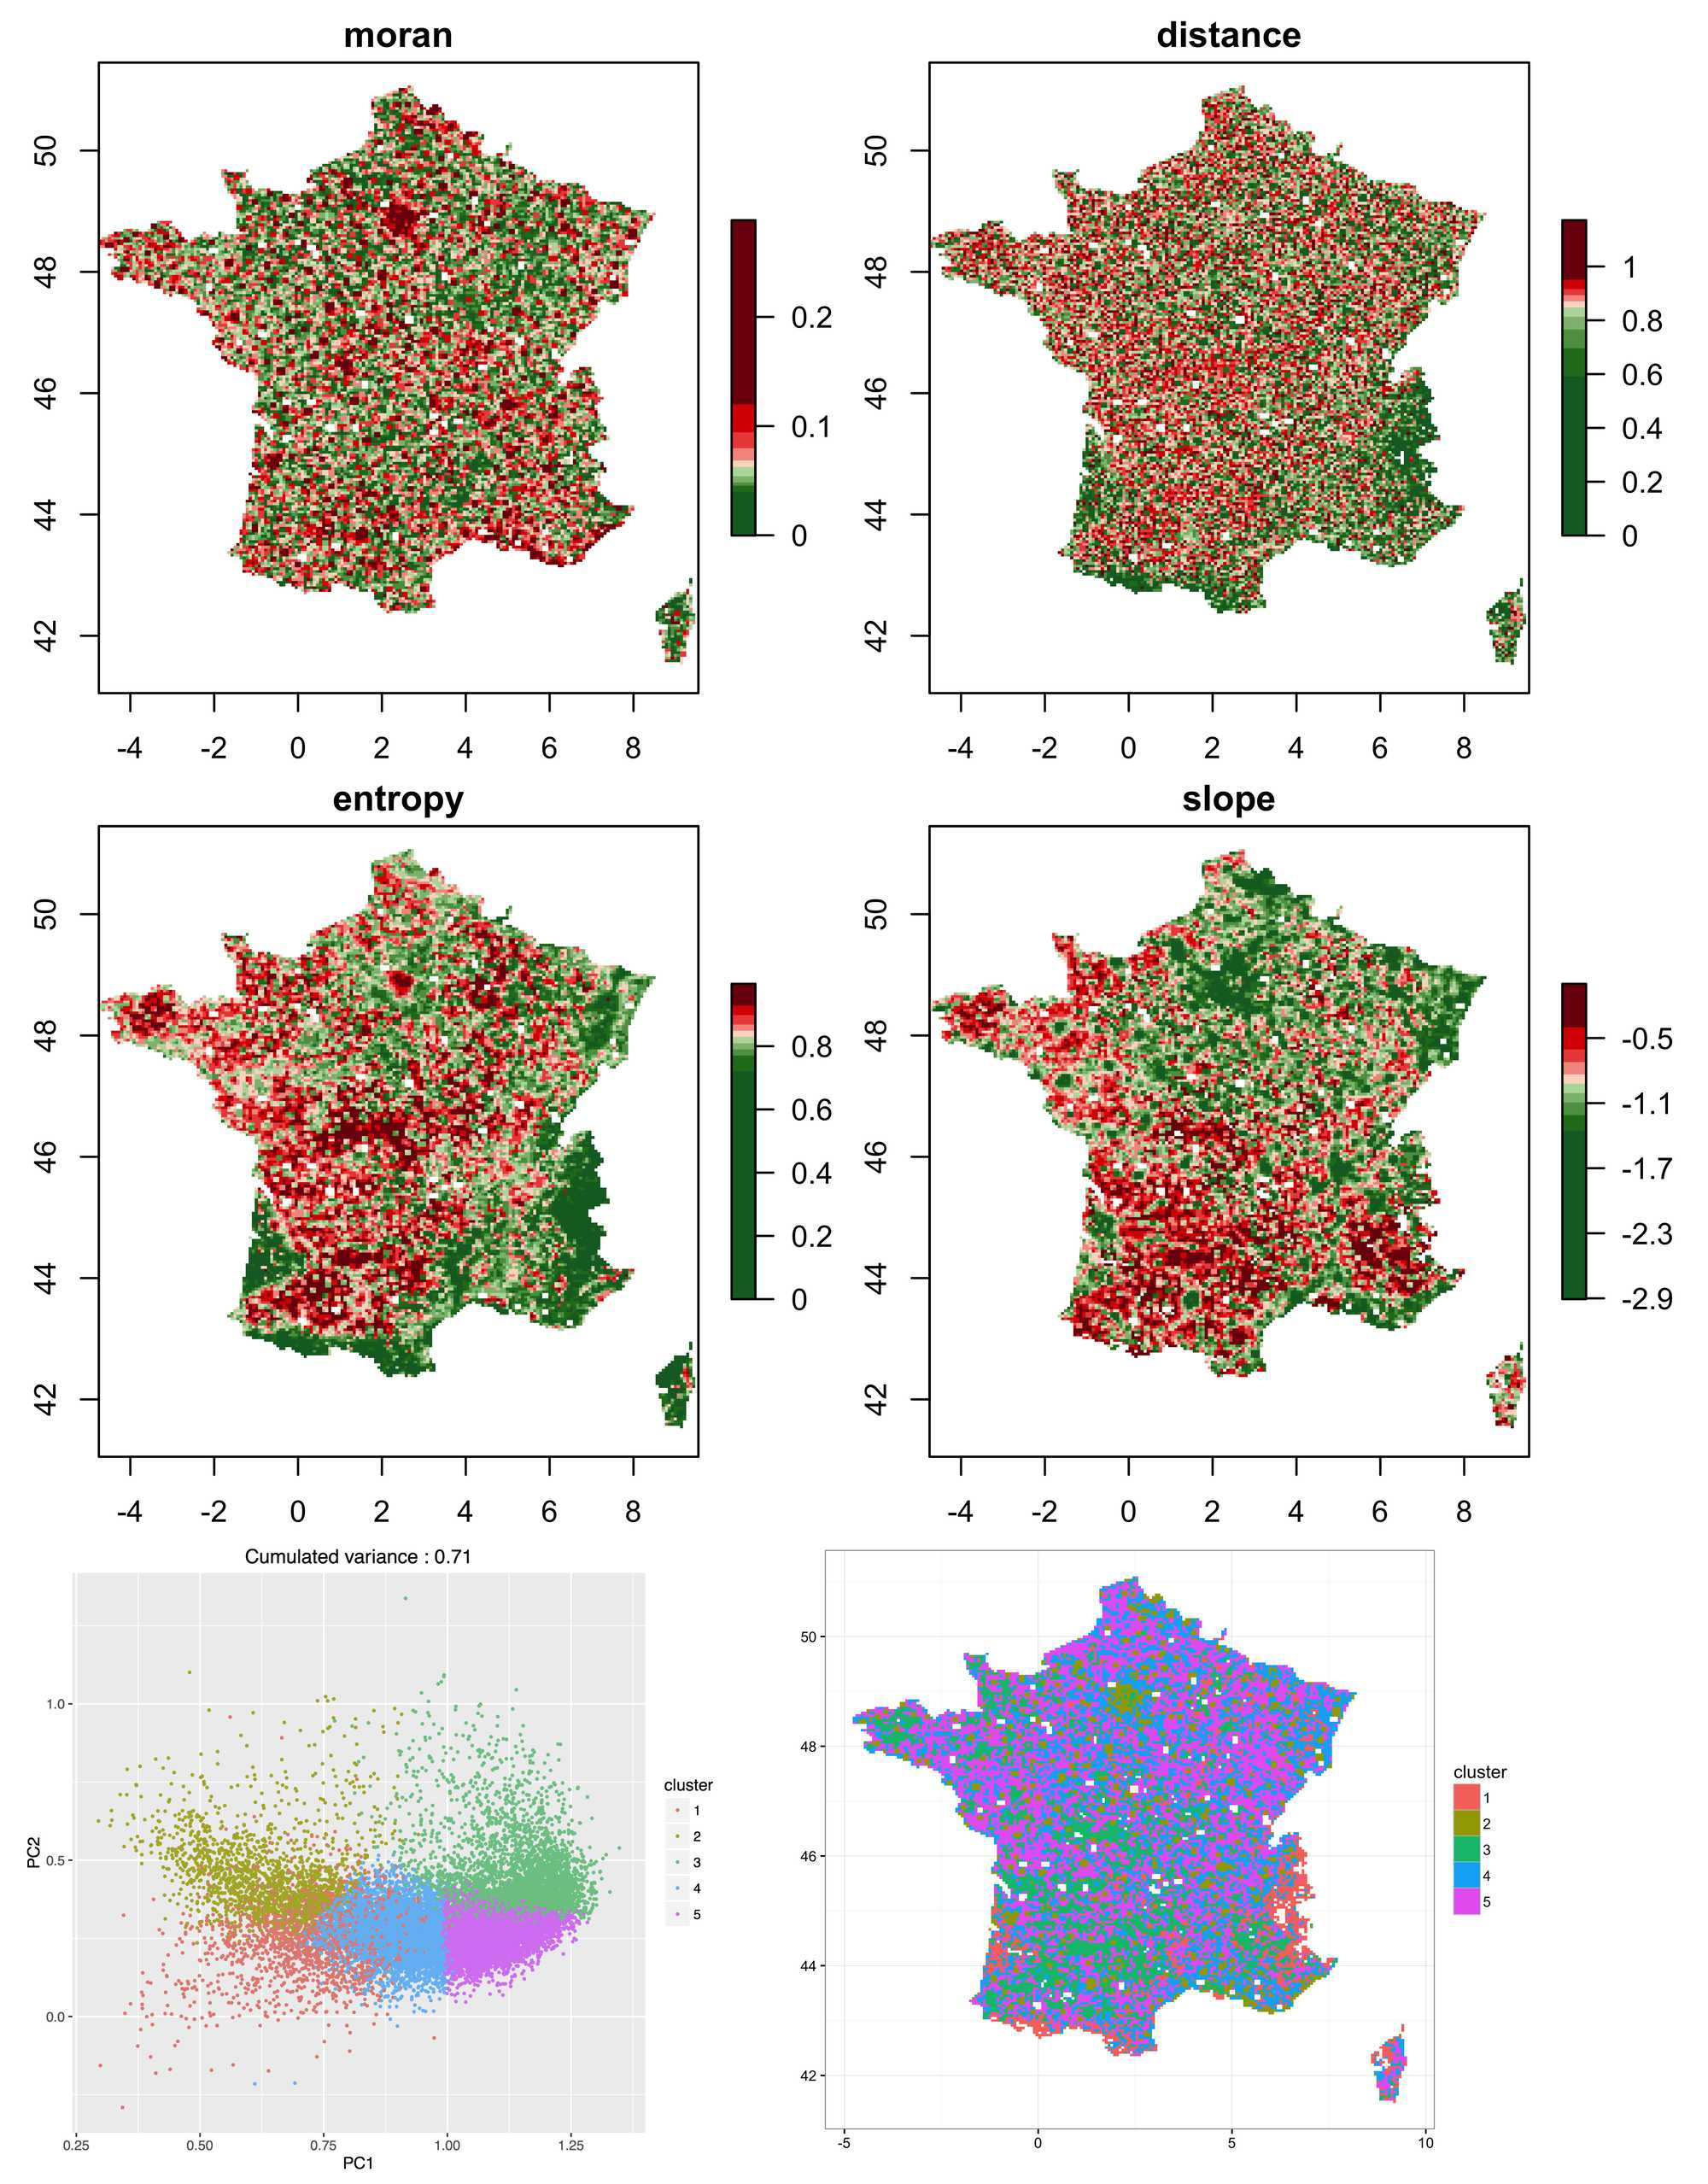
\includegraphics[width=0.9\linewidth]{Figures/Final/4-1-1-fig-staticcorrelations-empirical}
%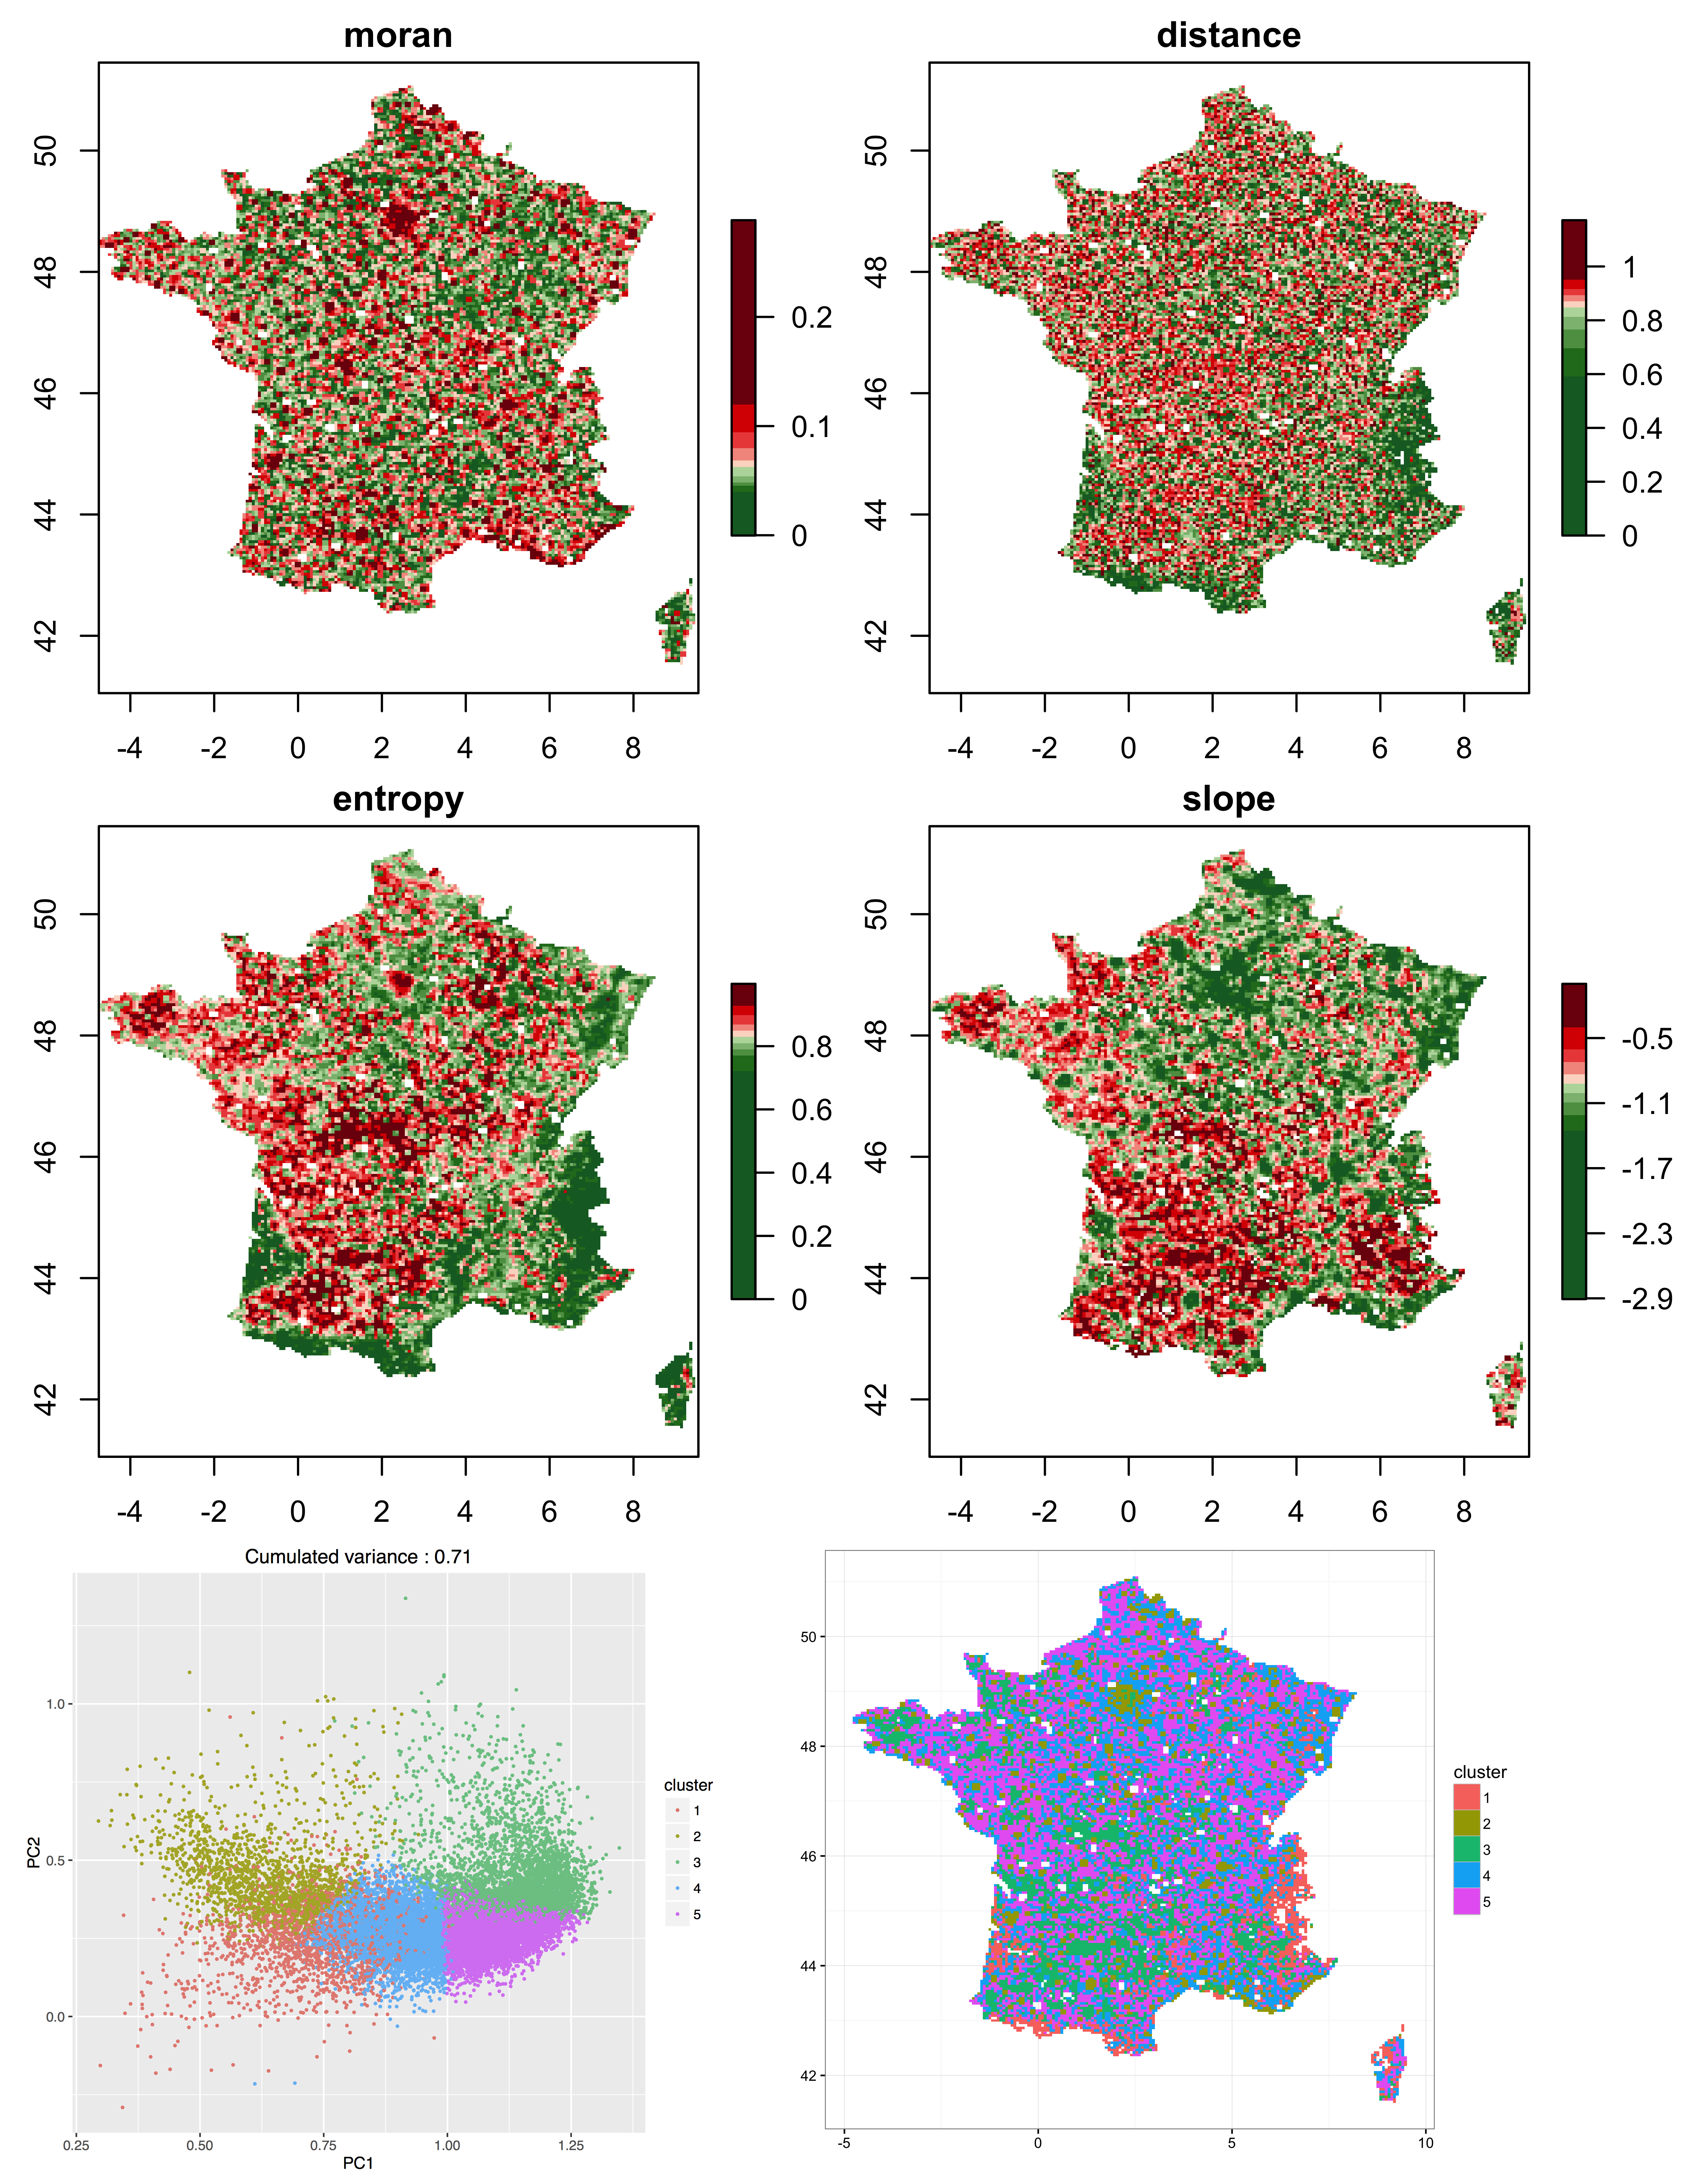
\includegraphics[width=0.9\linewidth]{Figures/Density/Fig1}
%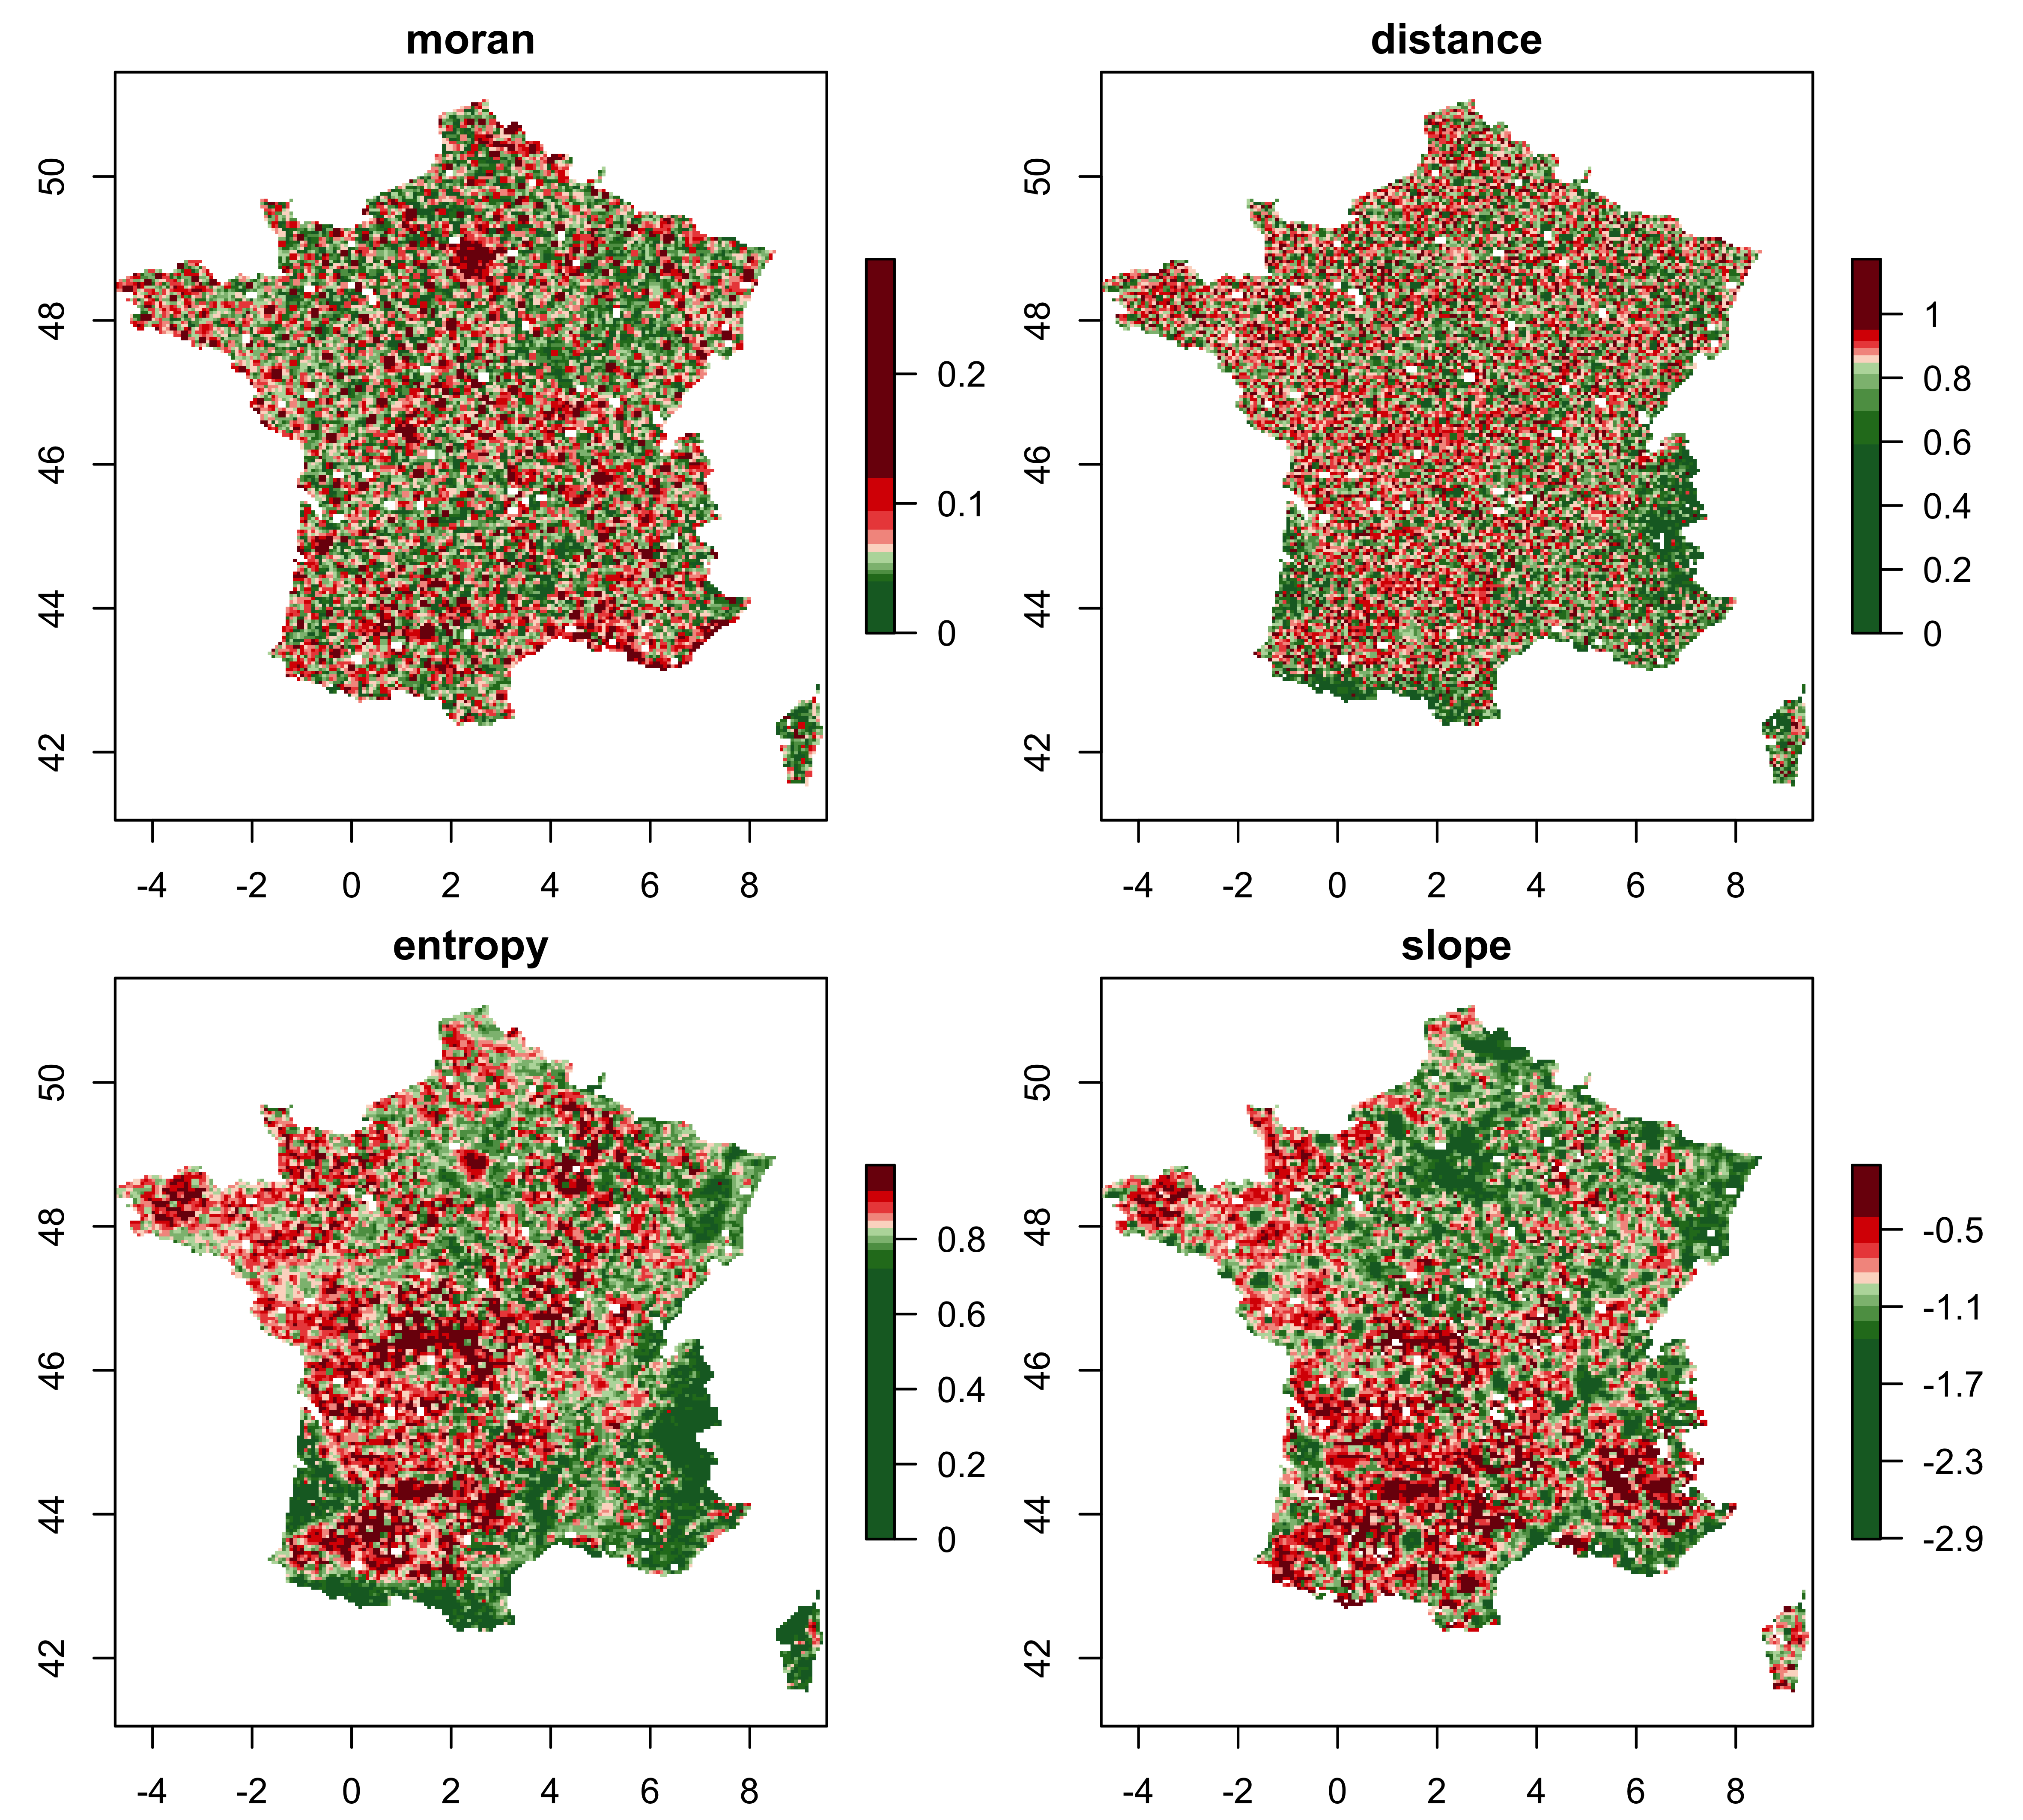
\includegraphics[width=\textwidth]{figures/indics_morpho_discrquantiles}\\
%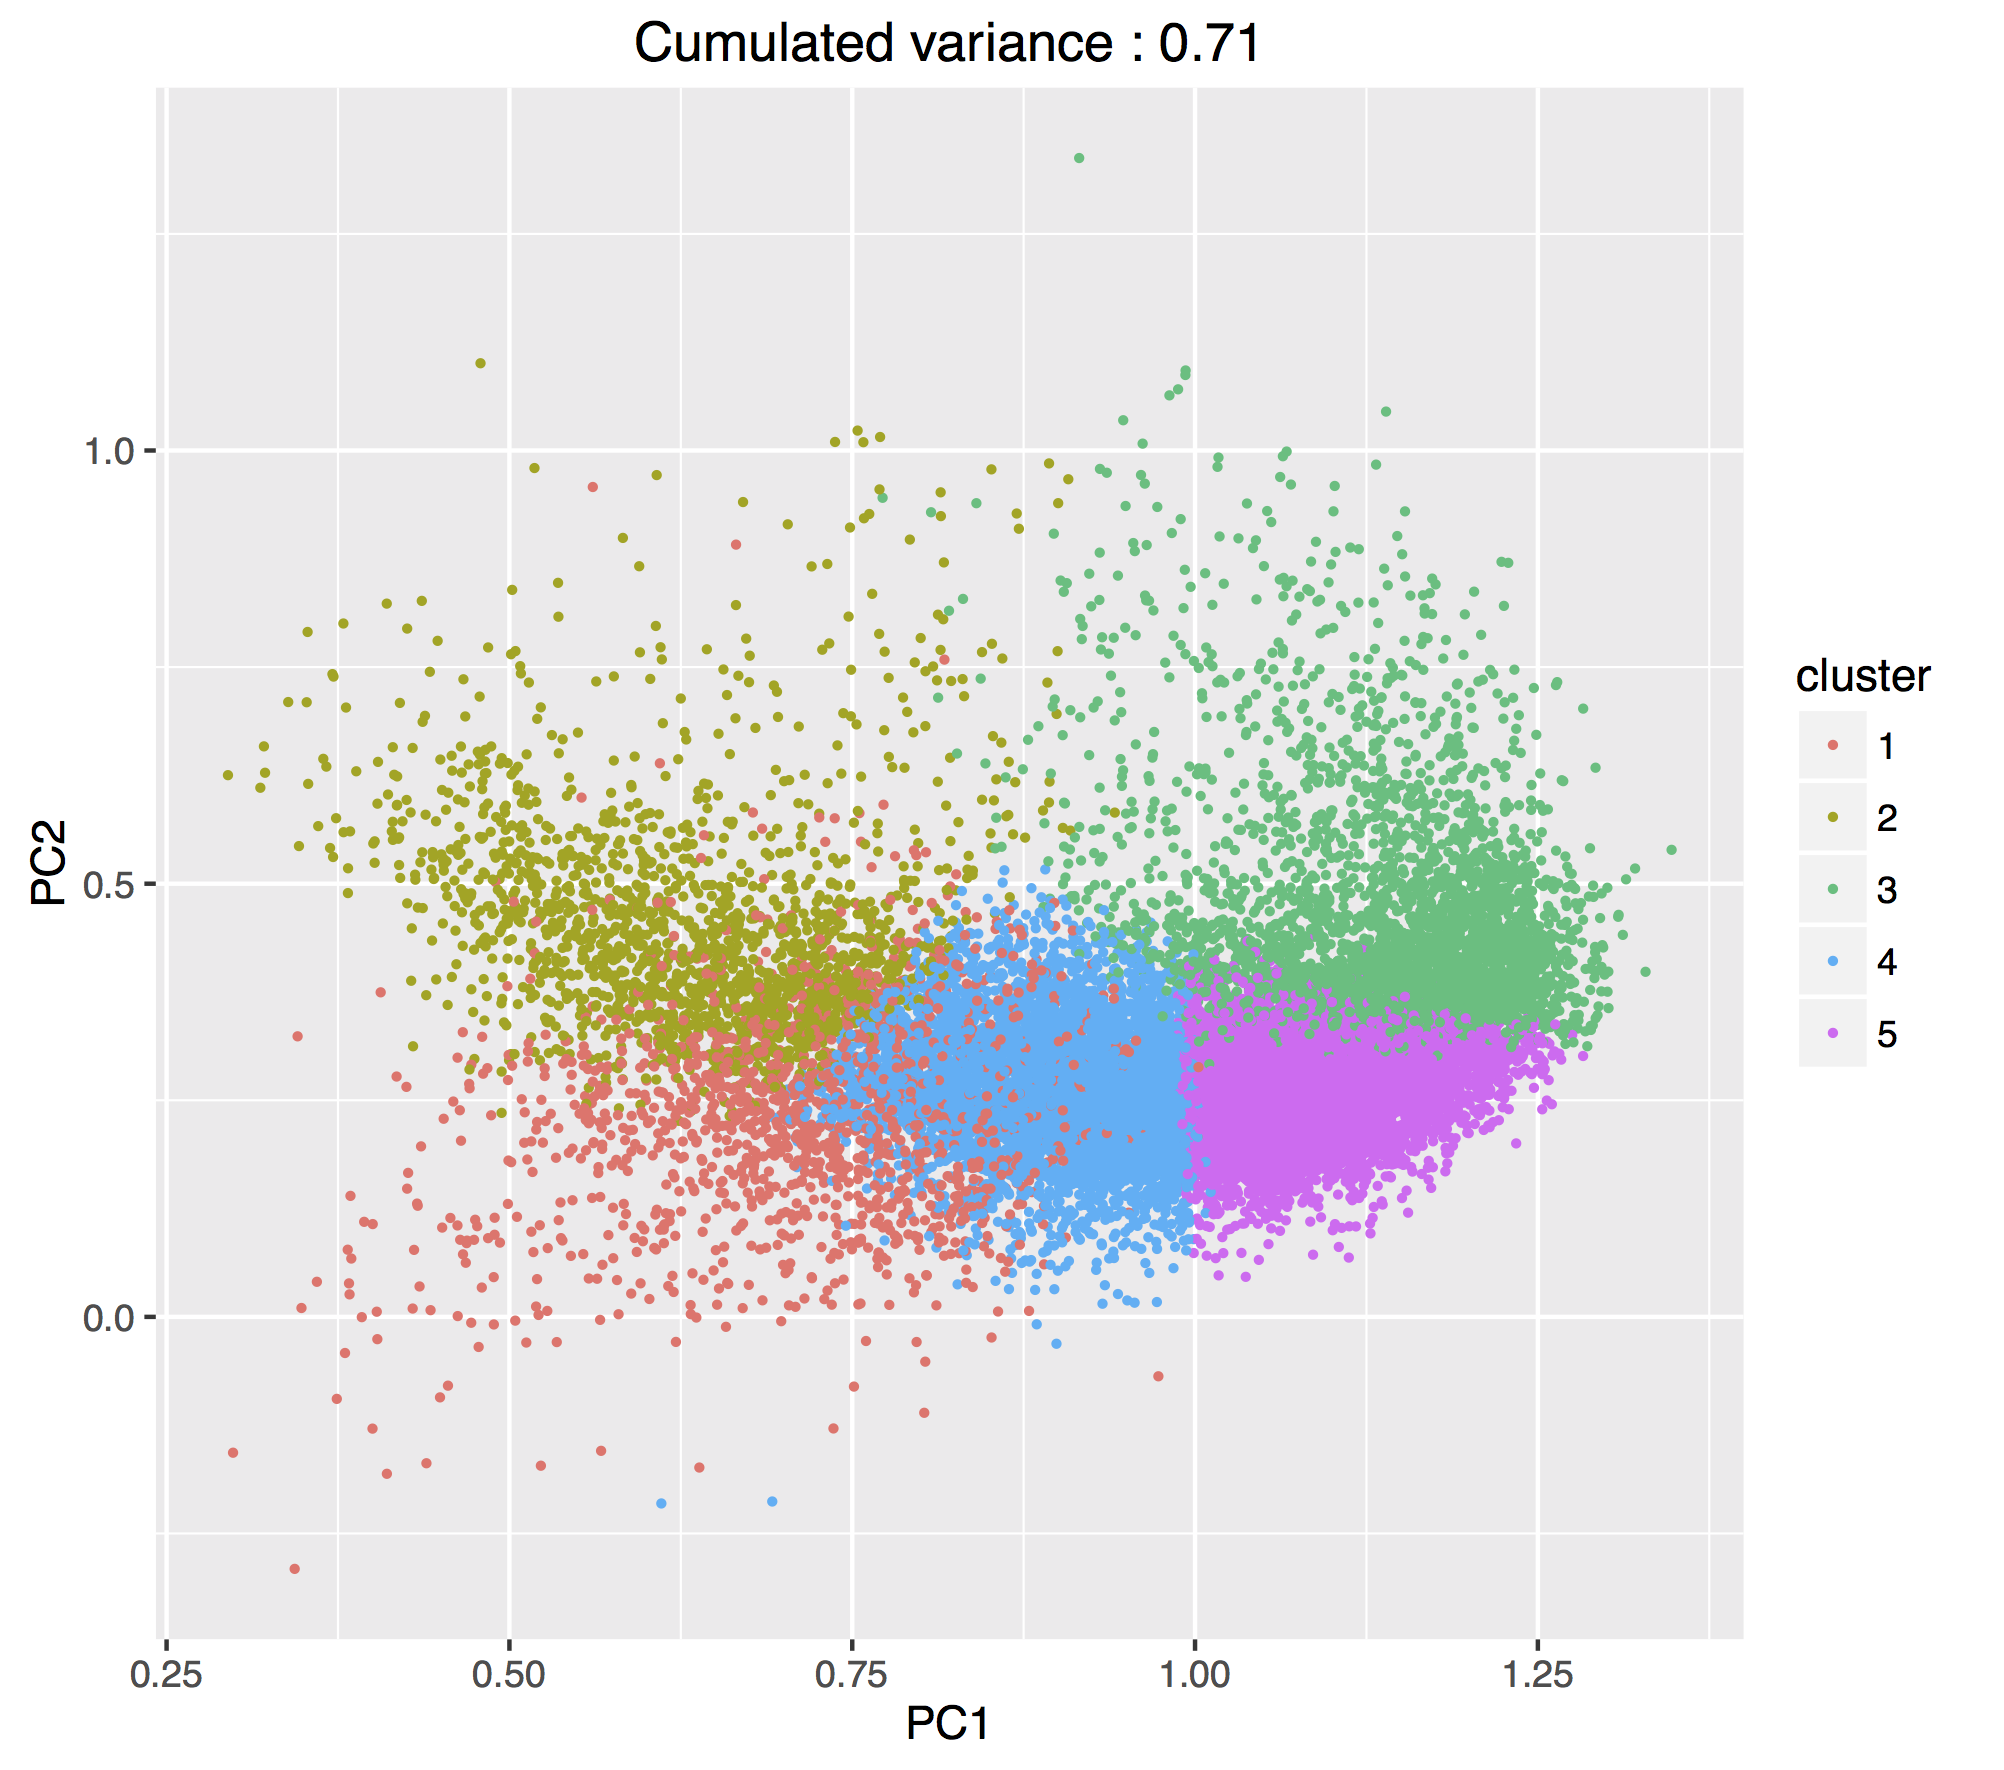
\includegraphics[width=0.49\textwidth]{figures/cluster_pca_k5_morpho}
%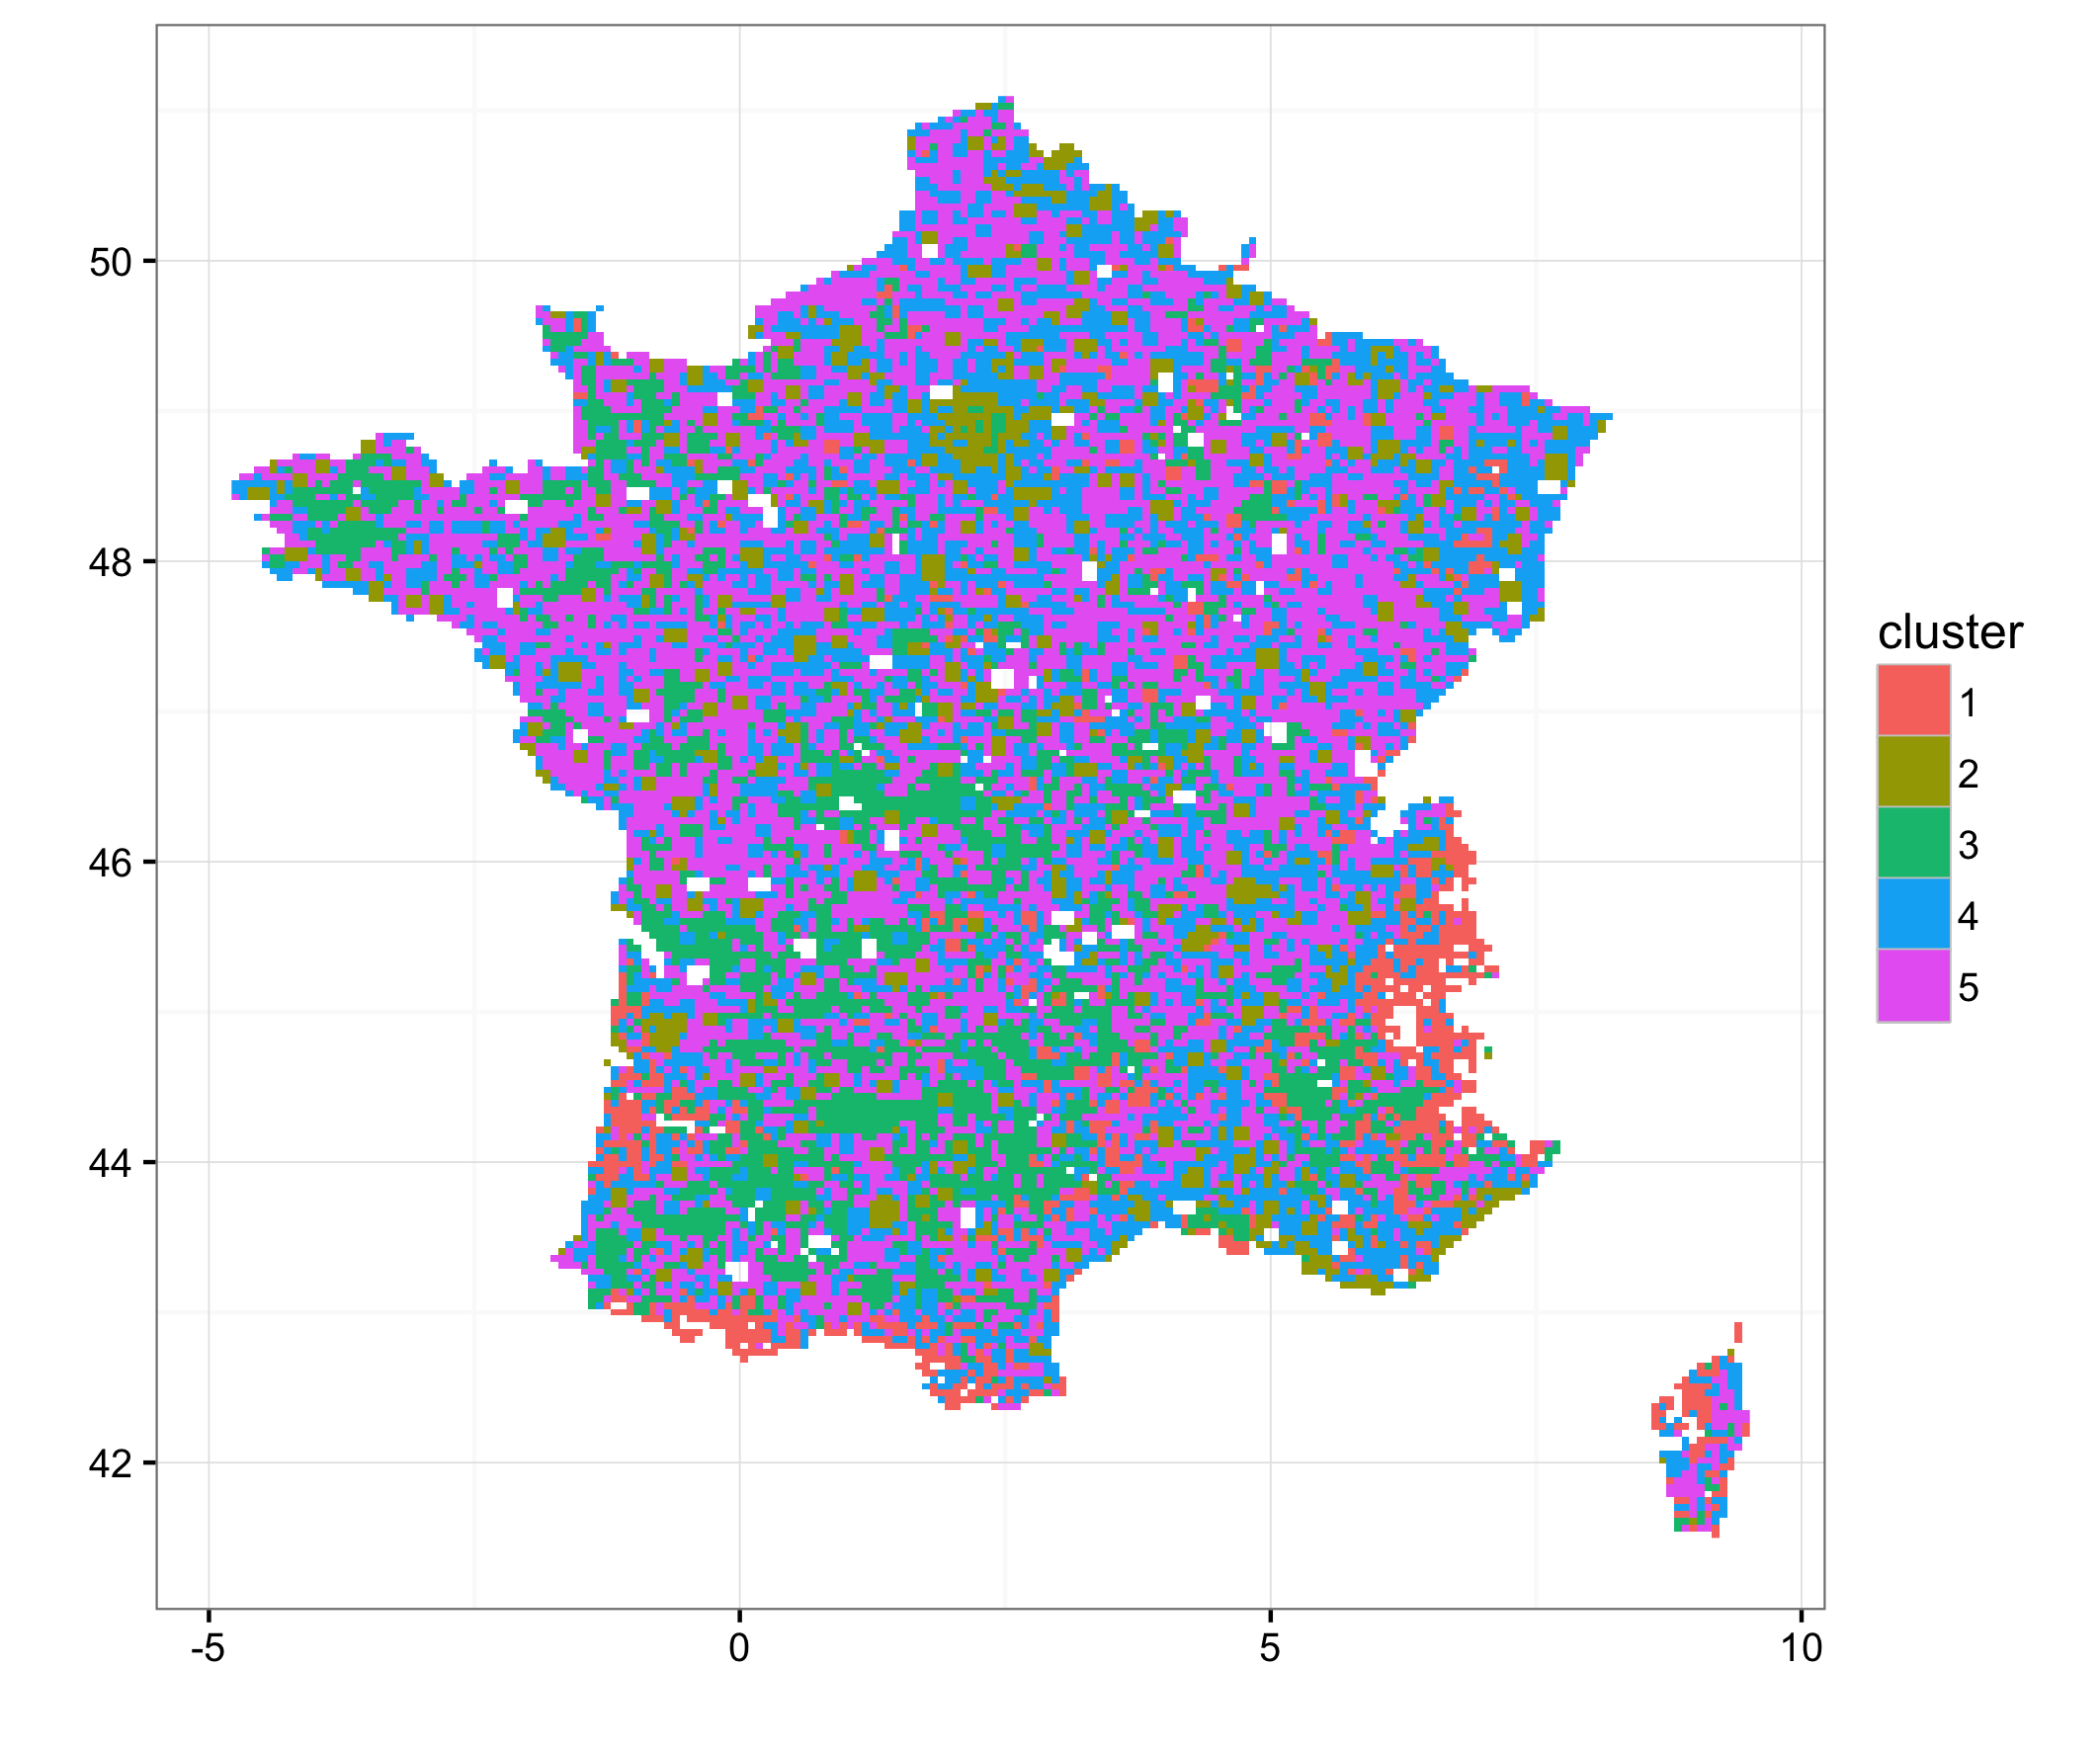
\includegraphics[width=0.49\textwidth]{figures/cluster_map_k5_morpho}
\caption[Empirical values of morphological indicators][Distribution spatiale des morphologies]{\textbf{Empirical values of morphological indicators.} \textit{(Top four maps)} Spatial distribution of the morphological indicators for France. Scale color discretization is done using quantiles to ease map readability. \textit{(Bottom Left)} Projection of morphological values on the two first components on a Principal Component analysis. Color gives cluster in an unsupervised classification (see text). \textit{(Bottom right)} Spatial distribution of clusters.\label{fig:staticcorrelations:empirical}}{\textbf{Valeurs empiriques des indicateurs morphologiques.} \textit{(Quatre cartes du haut)} Distribution spatiale des indicateurs morphologiques pour la France. La détermination de l'échelle de couleur est faite par quantiles pour faciliter la lecture des cartes. \textit{(Bas gauche)} Projection des valeurs morphologiques sur les deux premières composantes d'une analyse en composantes principales. La couleur donne le cluster dans une classification non supervisée (voir texte). \textit{(Bas droite)} Distribution spatiale des clusters. Se référer au texte pour les détails sur la procédure d'estimation spatiale des indicateurs et sur la procédure de classification.\comment[FL]{ta distribution n'est pas centree $\rightarrow$ quelle interpretation tires tu de ce choix ? ; legende ? ; attention aux echelles de couleur ; traduire ; a ce stade le lecteur peut se dire `` pour lui un territoire = 1 carre de 100km de cote $\rightarrow$ a priori il sera sceptique : tu dois donc defendre ta posture avec une particuliere clarté}\label{fig:staticcorrelations:empirical}}
\end{figure}
%%%%%%%%%%%%%%%%%%%%%%%%

%\comment[FL]{a quelle distance se fait la fenetre ? par ailleurs le gros pb est que tu ne parles pas de ville ; ce n'est pas lisible $\rightarrow$ montrer moins de resultats filtres.}


\bpar{
We compute the morphological measures given above on real urban density data, using the population density grid of the European Union at 100m resolution provided openly by Eurostat~\cite{eurostat}. The choice of the resolution, the spatial range, and the shape of the window on which indicators are computed, is made according to the thematic specifications given before. We consider 50km wide square windows to be in accordance with the expected spatial range of one model instance. As it also does not make sense to have a too detailed resolution because of data quality, we take $N=100$ and aggregate the initial raster data at a 500m resolution to meet this size on real windows. To have a rather continuous distribution of indicators in space, we overlap windows by setting an offset of 10km between each, what also somehow rules out the question of window shape bias by the ``continuity'' of values. We tested the sensitivity to window size by computing samples with 30km and 100km window sizes and obtained rather similar spatial distributions. We show in Fig.~\ref{fig:staticcorrelations:empirical} maps giving values of indicators for France only to ease maps readability. The first striking feature is the diversity of morphological patterns across the full territory. The auto-correlation is naturally high in Metropolitan areas, with the Parisian surroundings clearly detached. When looking at other indicators, it is interesting to denote regional regimes: rural areas have much less hierarchy in the South than in the North, whereas the average distance is rather uniformly distributed except for mountain areas. Regions of very high entropy are observed in the Center and South-West. To have a better insight into morphological regimes, we use unsupervised classification with a simple k-means algorithm, for which the number of clusters $k=5$ witnesses a transition in inter-cluster variance. The split between classes is plotted in Fig.~\ref{fig:empirical}, bottom-left panel, where we show measures projected on the two first components of a Principal Component Analysis (explaining 71\% of variance). The map of morphological classes confirms a North-South opposition in a background rural regime (clear green against blue), the existence of mountainous (red) and metropolitan (dark green) regimes. Such a variety of settlements forms will be the target for the model. We did similar analysis for China using the gridded population data from~\cite{fu1km}: maps are available in~\ref{app:sec:staticcorrelations}.
}{
Nous calculons les mesures morphologiques données ci-dessus sur des données réelles de densité, en utilisant la grille de population de l'Union Européenne à la résolution de 100m fournie de manière ouverte par Eurostat~\cite{eurostat}. Cette base a certains défauts de précision qui ont été reconnus~\cite{bretagnolle2016ville} mais nous agrégerons les données à un niveau suffisant pour les éviter.\comment[FL]{est-ce que le lecteur doit te croire sur parole ? il faut en dire un peu plus} Le choix de la résolution, de la portée spatiale, et de la forme de la fenêtre sur laquelle les indicateurs sont calculés, sont faits suivant les spécifications thématiques précédentes. Nous considérons des fenêtres carrées de largeur 50km, ce qui permet de plus d'être en accord avec l'ontologie du modèle de morphogenèse que l'on développera en~\ref{sec:densitygeneration}.\comment[FL]{cette justification est tres courte et non acceptable car elle renvoie a la suite. en plus c'est vraiment un des points les plus discutables de ton approche : tu ne peux pas te permettre a eluder ainsi cette question} Comme une résolution trop détaillée n'est pas désirable à cause de la qualité des données, nous agrégeons les données raster\comment[FL]{sens ?} initiales à une résolution de 500m pour avoir des fenêtres de taille $N=100$.\comment[FL]{ok 50km = 500m x 100 mais tu n'aides pas vraiment ton lecteur} Pour obtenir une distribution des indicateurs relativement continue dans l'espace, nous superposons les fenêtres en posant un décalage de 10km entre chaque, ce qui d'une certaine façon\comment[FL]{c'est trop flou : c'est un gros travail pourtant et pas du tout valorise} résout le problème du biais de la forme de la fenêtre par la ``continuité'' des valeurs. Nous avons testé la sensibilité à la taille de la fenêtre en calculant des échantillons avec des tailles de 30km et 100km et avons obtenu des distributions spatiales assez similaires.\comment[FL]{la encore : faut-il te croire sur parole ? qu'as tu regarde precisement ?} L'implémentation des indicateurs doit être faite avec attention, puisque les complexités computationnelles peuvent atteindre $O(N^4)$ pour l'indice de Moran par exemple: nous utilisons la convolution par Transformée de Fourier Rapide, qui est une technique permettant de calculer l'indice de Moran avec une complexité en $O(\log^2 N \cdot N^2)$\comment[FL]{ce n'est pas comprehensible par tout le monde}[(JR) ok rajouter un paragraphe complexite algo dans le prelim math]. Nous montrons en Fig.~\ref{fig:staticcorrelations:empirical} des cartes donnant les valeurs des indicateurs, pour la France seulement afin de permettre une lisibilité. Les distributions empiriques pour chaque indicateur sont données en Appendice~\ref{app:sec:staticcorrelations}. La première caractéristique frappante est la diversité des motifs morphologiques au travers de l'ensemble du territoire. L'auto-correlation est relativement haute dans les zones métropolitaines\comment[FL]{sens ? tu n'as pas defini cela}, avec les environs de Paris qui se détachent clairement. Lorsqu'on s'intéresse aux autres indicateurs, il est intéressant de constater des régimes régionaux: les zones rurales ont beaucoup moins de hiérarchie dans le Sud que dans le Nord\comment[FL]{pas essentiel a mon avis cette discussion}, tandis que la distance moyenne est plutôt distribuée uniformément sauf dans les zones montagneuses.\comment[FL]{c'est une propriete macro $\rightarrow$ c'est curieux que cela vienne apres les c artes de France (qui sont tres detaillees)} Des régions qui présentent de fortes valeurs de l'entropie sont observées dans le centre et le Sud-ouest. Pour avoir une meilleure compréhension des classes morphologiques existantes, nous utilisons une classification non-supervisée\footnote{Qui consiste à partitioner l'espace des données selon leur structure endogène.} avec un algorithme des k-means\comment[FL]{sens ?} simple. \comment{\cite{goerlich2017clustering} : variable prises en compte, ne pas prendre pop sinon catégories pas intéressantes comme ce papier}
 Le nombre de clusters $k=5$ induit une transition dans la variance inter-cluster, ce qui signifie qu'une variation de structure opère à ce nombre,\comment[FL]{tu pourrais au moins une fois detailler les procedures que tu utilises. le lecteur doit pouvoir se faire sa propre idee : est-tu ``bon'' dans le traitement des donnes ou ``moyen'' Pas de raison d'etre confiant a priori} que nous choisissons alors comme nombre de clusters. La séparation entre les classes est montrée en~\ref{fig:staticcorrelations:empirical}, panneau bas gauche, où nous représentons les mesures projetées sur les deux premières composantes d'une Analyse en Composantes Principales (expliquant 71\% de la variance, ce qui est relativement conséquent). La carte des classes morphologiques confirme une opposition Nord-Sud dans le régime rural de fond (vert clair contre bleu), l'existence d'un régime de montagne (rouge) et d'un régime métropolitain (vert sombre)\comment[FL]{est-ce tout ce que tu peux montrer ? N/S x urbain/rural ? dans ce cas quel apport de ta methodologie ? je pense que cela merite des developpements}. Une telle variété d'établissements sera l'un des objectifs du modèle en~\ref{sec:densitygeneration}. Un calcul similaire des indicateurs morphologiques a été effectué pour la Chine en utilisant la grille de population à 1km fournie par~\cite{fu1km}. Les cartes sont disponibles en Appendice~\ref{app:sec:staticcorrelations}.
}


%%%%%%
% Correlation entre 50km smoothé et 100km (idem 30km) pour quantifier sensibilite a la taille de la fenetre. forme : calcul de coin de table avec smoothing.
% -> cf appendice sur sensitivity a la resolution






%%%%%%%%%%%%%%%%%%
\subsection{Network Measures}{Mesures de Réseau}


\bpar{
We consider network aggregated indicators as a way to characterize transportation network properties on a given territory, the same way morphological indicators yielded information on urban structure. We propose to compute some simple indicators on same extents as for morphology, to be able to explore relations between these static measures.
}{
Nous considérons d'autre part les mesures agrégées de réseau comme un moyen de caractériser les propriétés des réseaux de transport sur un territoire donné, de la même façon que les indicateurs morphologiques informent sur la structure urbaine. Nous proposons de calculer des indicateurs simples sur des étendues spatiales similaires à celles retenues pour la mesure de la morphologie, pour être en mesure d'explorer les relations entre ces mesures statiques.
}

\bpar{
Static network analysis has been extensively documented in the literature, see for example \cite{louf2014typology} for a cross-sectional study of cities or \cite{2015arXiv151201268L} for exploration of new measures for the road network.
}{
L'analyse statique de réseau a été intensément documentée dans la littérature, voir par example \cite{louf2014typology} pour une étude comparative des villes ou \cite{2015arXiv151201268L} pour l'exploration de nouvelles mesures pour le réseau de rues. \cite{2017arXiv170902939M} utilise des techniques issues de l'apprentissage profond pour établir une typologie des réseaux viaires urbains pour un grand nombre de villes dans le monde. Les enjeux derrière ce genre d'approches sont multiples : elles peuvent viser à des typologies ou caractérisations de réseaux spatiaux, à des compréhensions des processus dynamiques sous-jacents dans un but de modélisation de la morphogenèse, ou même de planification urbaine comme sont appliquées parfois les approches par \emph{Space Syntax}~\cite{hillier1989social}. Nous nous plaçons ici plutôt dans les deux premières logiques. Notre contribution significative est la caractérisation du réseau routier sur de grandes étendues spatiales, couvrant l'Europe et la Chine.
}


\subsubsection{Data preprocessing}{Pré-traitement des données}


\bpar{
We work here with the road network, which structure is finely conditioned to territorial configuration of population densities. Furthermore, data for present day road network is openly available through the OpenStreetMap project~\cite{openstreetmap}. Its quality was investigated for different countries such as England~\cite{haklay2010good} and France~\cite{girres2010quality}. It was found to be of a quality equivalent to official surveys for the primary road network. Concerning China, although \cite{zheng2014assessing} underlined a quick acceleration of OpenStreetMap road data completeness and accuracy, its use for computation of network indicators may be questioned at a very fine scale. \cite{zhang2015density} highlights four regimes of data quality, partitioning China into regions among which qualitative behavior of OSM data varies. We underline that the results will be more valid on the regions where the quality is the highest, i.e. with high density and high diversity.
}{
Nous travaillons ici avec le réseau de rues, dont la structure est finement conditionnée aux configurations territoriales des densités de population. De plus, les données du réseau de routes actuel est disponible ouvertement par l'intermédiaire du projet OpenStreetMap (OSM)~\cite{openstreetmap}. Sa qualité a été étudiée pour différents pays comme l'Angleterre~\cite{haklay2010good} et la France~\cite{girres2010quality}. Il a été établi pour ces pays une qualité équivalente aux données officielles pour le réseau de rues primaire, au sens à la fois de la couverture spatiale et de la précision locale. Dans le cas de la Chine, bien que \cite{zheng2014assessing} soulève une récente accélération de la couverture et de la précision des données OSM pour les routes, leur usage pour le calcul d'indicateurs de réseau peut être questionné à une échelle très fine. \cite{zhang2015density} fournit une partition de la Chine en régions entre lesquelles le comportement qualitatif des données OSM varie. Nous devrons garder à l'esprit cette variabilité, et pour être assuré de la fiabilité des résultats, nous simplifierons le réseau à un niveau d'agrégation suffisant.
}




\bpar{
From the primary road segments, we compute the topological road network for all studied areas, at 100m granularity scale to be used consistently with the population grid. The OSM data is imported into \texttt{pgsql} using \texttt{osmosis}, is then aggregated at fixed granularity, and the resulting topological network is finally simplified with a split/merge algorithm. We have for Europe $\simeq 44\cdot 10^6$ links in initial OSM db, $\simeq 61\cdot 10^6$ in first simplified layer, $\simeq 21\cdot 10^6$ in final database. For a given dataset corresponding to a subset of the overall road network, it is necessary to simplify network structure by spatial aggregation as initial data presents very detailed features and thus a very large numbers of nodes ($\simeq 10^10$ for Europe dataset). It is possible to drastically reduce network size by spatial aggregation of nodes and link replacements. The detailed algorithm and implementation are detailed in Supplementary material~\ref{app:sec:staticcorrelations}.
}{
Pour les segments de rue primaires, nous calculons le réseau topologique pour l'ensemble des zones étudiées, à une granularité de 100m pour pouvoir être utilisé de manière cohérente avec les grilles de population et pour être robuste aux imperfections locales de codage ou données très locales manquantes.\comment[FL]{d'ou provient ce seuil ? as tu fait des essais alternatifs ?} Les données OSM sont importées dans une base de données \texttt{pgsql} en utilisant le logiciel \texttt{osmosis}~\cite{osmosis}.
}

\bpar{}{
Le réseau est ensuite agrégé à la granularité fixe pour créer un graphe topologique, qui est finalement simplifié pour garder uniquement la structure topologique du réseau, les indicateurs normalisés étant relativement robustes à cette opération. Celle-ci est nécessaire pour un calcul simple des indicateurs et une cohérence thématique avec la couche de densité. On garde uniquement les noeuds ayant un degré strictement supérieur ou inférieur à deux, et les liaisons correspondantes, en prenant soin d'agréger la distance géographique réelle en construisant le lien topologique correspondant. Vu l'ordre de grandeur de taille des données (pour l'Europe, la base initiale a $\simeq 44.7\cdot 10^6$ liens, et la base finale simplifiée $\simeq 20.4\cdot 10^6$), un algorithme spécifique parallèle est mis en place, de structure \emph{split-merge}. Celui-ci découpe l'espace en zones qui peuvent être traitées indépendamment puis fusionnées. Il est détaillé en Appendice~\ref{app:sec:staticcorrelations}.
}



%china 2048589 ; simpl 2022802
%europe 44706945 ; simpl 20443061

\subsubsection{Indicators}{Indicateurs}

\bpar{
These indicators are used to capture a rough picture of the structure. Refined work at smaller scales (intra-urban road network) and with more elaborated measures that allow to differentiate more precisely local form, was recently done by Lagesse in~\cite{2015arXiv151201268L}.
Network macroscopic structure is summarized by the following set of indicators, after the simplifications and reductions done in the previous step. Assuming network given by $N=(V,E)$, nodes spatial positions $\vec{x}(V)$ and edges \emph{effective distances} $d(E)$ taking into account impedances and real distances (to include basically network hierarchy), we have indicators:
}{
Nous introduisons des indicateurs pour avoir une idée large de la forme du réseau, utilisant un certain nombre d'indicateurs pour capturer le maximum de dimensions des propriétés des réseaux, plus ou moins liées à l'utilisation de ceux-ci. Ces indicateurs résumant la structure mesoscopique du réseau sont calculés sur les réseau topologiques obtenus par les étapes précédentes de simplification. Notant le réseau $N=(V,E)$, les noeuds $V$ ont des positions spatiales $\vec{x}(v)$ et des populations $p(v)$ obtenues par agrégation de la population dans la partition de Dirichlet correspondante, les liens $E$ ont des \emph{distances effectives} $l(E)$ qui prennent en compte les impédances et les distances réelles (pour inclure la hiérarchie primaire du réseau). Nous utilisons alors :
}

%"vcount"      "ecount" "gamma"   "meanDegree"   "mu"  "alpha"        "meanLinkLength"     "meanNodePop"        "meanClustCoef"      "components"        "meanBetweenness"    "alphaBetweenness"   "euclPerf"           "diameter"        "meanCloseness"      "alphaCloseness.x"   "meanTravelTime"     "alphaTravelTime.x"  "alphaAccessibility" "meanAccessibility"  "modularity"

\bpar{
\begin{itemize}
\item connectivity
\item degree distribution
\item centrality, taken as normalized mean \emph{betweenness-centrality}
\item average path length
\item network diameter
\item mean network speed
\end{itemize}
}{
\begin{itemize}
\item Caractéristiques du graphe, issues de la théorie des graphes, comme définies par~\cite{haggett1970network} : nombre de noeuds $\left|V\right|$, nombre de lien $\left|E\right|$, densité $d$, degré moyen $\bar{\delta}$, nombre cyclotomique $\mu$, connectivité $\alpha$, longueur moyenne des liens $\bar{l}$, population moyenne $\bar{p}$, coefficient de clustering moyen $\bar{c}$, nombre de composantes $c_0$.
\item Mesures liées au plus courts chemins : diamètre $r$, performance euclidienne (définie par~\cite{banos2012towards}).
\item Mesures de centralité : celles-ci sont agrégées au niveau du réseau en prenant leur moyenne et leur niveau de hiérarchie, calculé par un ajustement OLS d'une loi rang taille, pour les mesures de centralité suivantes :
\begin{itemize}
\item \emph{Betweenness Centrality}~\cite{crucitti2006centrality}, moyenne $\bar{bw}$ et hiérarchie $\alpha_{bw}$ : étant donné la distribution de la centralité sur l'ensemble des noeuds, on prend la pente d'un ajustement rang-taille ainsi que la moyenne de la distribution.
\item \emph{Closeness Centrality}~\cite{crucitti2006centrality}, moyenne $\bar{cl}$ et hiérarchie $\alpha_{cl}$
%\item Temps de trajet moyen vers les autres noeuds, moyenne $\bar{t}$ et hiérarchie $\alpha_{t}$ (prend en compte la vitesse maximale des liens) % pas utilisé finalement
\item Accessibilité~\cite{hansen1959accessibility}, qui est dans notre cas calculée comme une \emph{closeness} pondérée par les populations : moyenne $\bar{a}$ et hiérarchie $\alpha_{a}$
\end{itemize}
\item Modularité~\cite{blondel2008fast}, qui exprime la structure en communautés du réseau.
\end{itemize}
}

Le concept d'accessibilité est capturé ici par un indicateur de réseau, puisque son calcul implique d'attribuer des poids aux noeuds par un population correspondante, et revient ensuite à un temps de trajet moyen pondéré\comment[FL]{1) on a eu cette discussion au chap 1 $\rightarrow$c'est discutable 2) pas du tout logique que cela vienne apres la carte du chap 1 *(definition accessibilite)}. Cet indicateur est intéressant car à l'interface entre forme urbaine et forme du réseau, puisque la distribution de population sur les noeuds est prise en compte. On verra que celle-ci est fortement corrélée au même non-pondéré (corrélation de $\rho = 0.86$, estimée sur l'ensemble des points de mesure pour la Chine).




%%%%%%%%%%
%% -- ON HOLD -- (HS)

%\subsubsection{Network Shape and Resilience}{Forme de Réseau et Résilience}
%L'idée fondamentale motivant le calcul d'indicateurs de réseau est d'obtenir une réduction de dimension drastique, s'il est possible d'associer certains ``types'' de réseau à des valeurs typiques d'indicateurs. On est très loin d'une connaissance fine de typologies qui associeraient propriétés topologiques, dynamiques et processus de génération du réseau, le tout de manière synthétique. Il est de même difficile de relier systématiquement ces propriétés à des caractéristiques dérivées, comme par exemple pour la résilience qui est une propriété aux définitions diverses\footnote{Pour laquelle~\cite{Gao:2016ty} introduit une nouvelle approche par la sensibilité des processus dynamiques.}. Afin d'illustrer d'une part la difficulté de caractériser les réseaux et d'autre part les potentialités offertes par notre base de données, nous développons en Appendice~\ref{app:sec:staticcorrelations} une courte analyse des propriétés de résilience au sens de~\cite{ash2007optimizing} pour des réseaux typiques. Cette analyse fait, de la même manière que le calcul des indicateurs, partie d'une démarche générale de caractérisation des réseaux, essentielle ici comme préliminaire à l'étude de leur interaction avec les territoires.



\subsubsection{Results}{Résultats}


\bpar{}{
Les indicateurs de réseau ont été calculés sur les mêmes zones que les indicateurs de forme urbaine, pour pouvoir les mettre en correspondance directe et calculer les correlations par la suite. Nous montrons en Figure~\ref{fig:staticcorrs:network} un échantillon pour la France. Le comportement spatial des indicateurs est très instructif\comment[FL]{avant de discuter des resultats : presente les}, et révèle comme pour la forme urbaine des régimes locaux (urbain, rural, métropolitain), mais aussi des régimes régionaux très marqués. Ceux-ci peuvent être dus aux différentes pratiques agricoles selon les régions dans le cas du rural par exemple, impliquant une partition différente des parcelles ainsi qu'une organisation particulière de leur desserte. En taille du réseau, la Bretagne se détache nettement et rejoint les régions urbaines, témoignant de parcelles très fragmentées (et a fortiori d'un découpe foncière fragmentée également dans l'hypothèse simplificatrice d'une coincidence des parcelles et du foncier). Cela est partiellement corrélé à une faible hiérarchie dans l'accessibilité. Le Sud et l'Est du Bassin Parisien étendu se distinguent par une forte centralité d'intermédiarité moyenne, en accord avec une forte hiérarchisation du réseau. Pour la Chine, pour laquelle une selection d'indicateurs est également donnée en~\ref{app:sec:staticcorrelations}, on observe des variation locales et régionales encore plus marquées, ainsi que par exemple les mega-régions urbaines qui se détachent, correspondant à un régime bien particulier.\comment[FL]{tu n'as pas ammene ce cas d'etude}
}




%%%%%%%%%%%%%%%%%%%%%%%%
\begin{figure}
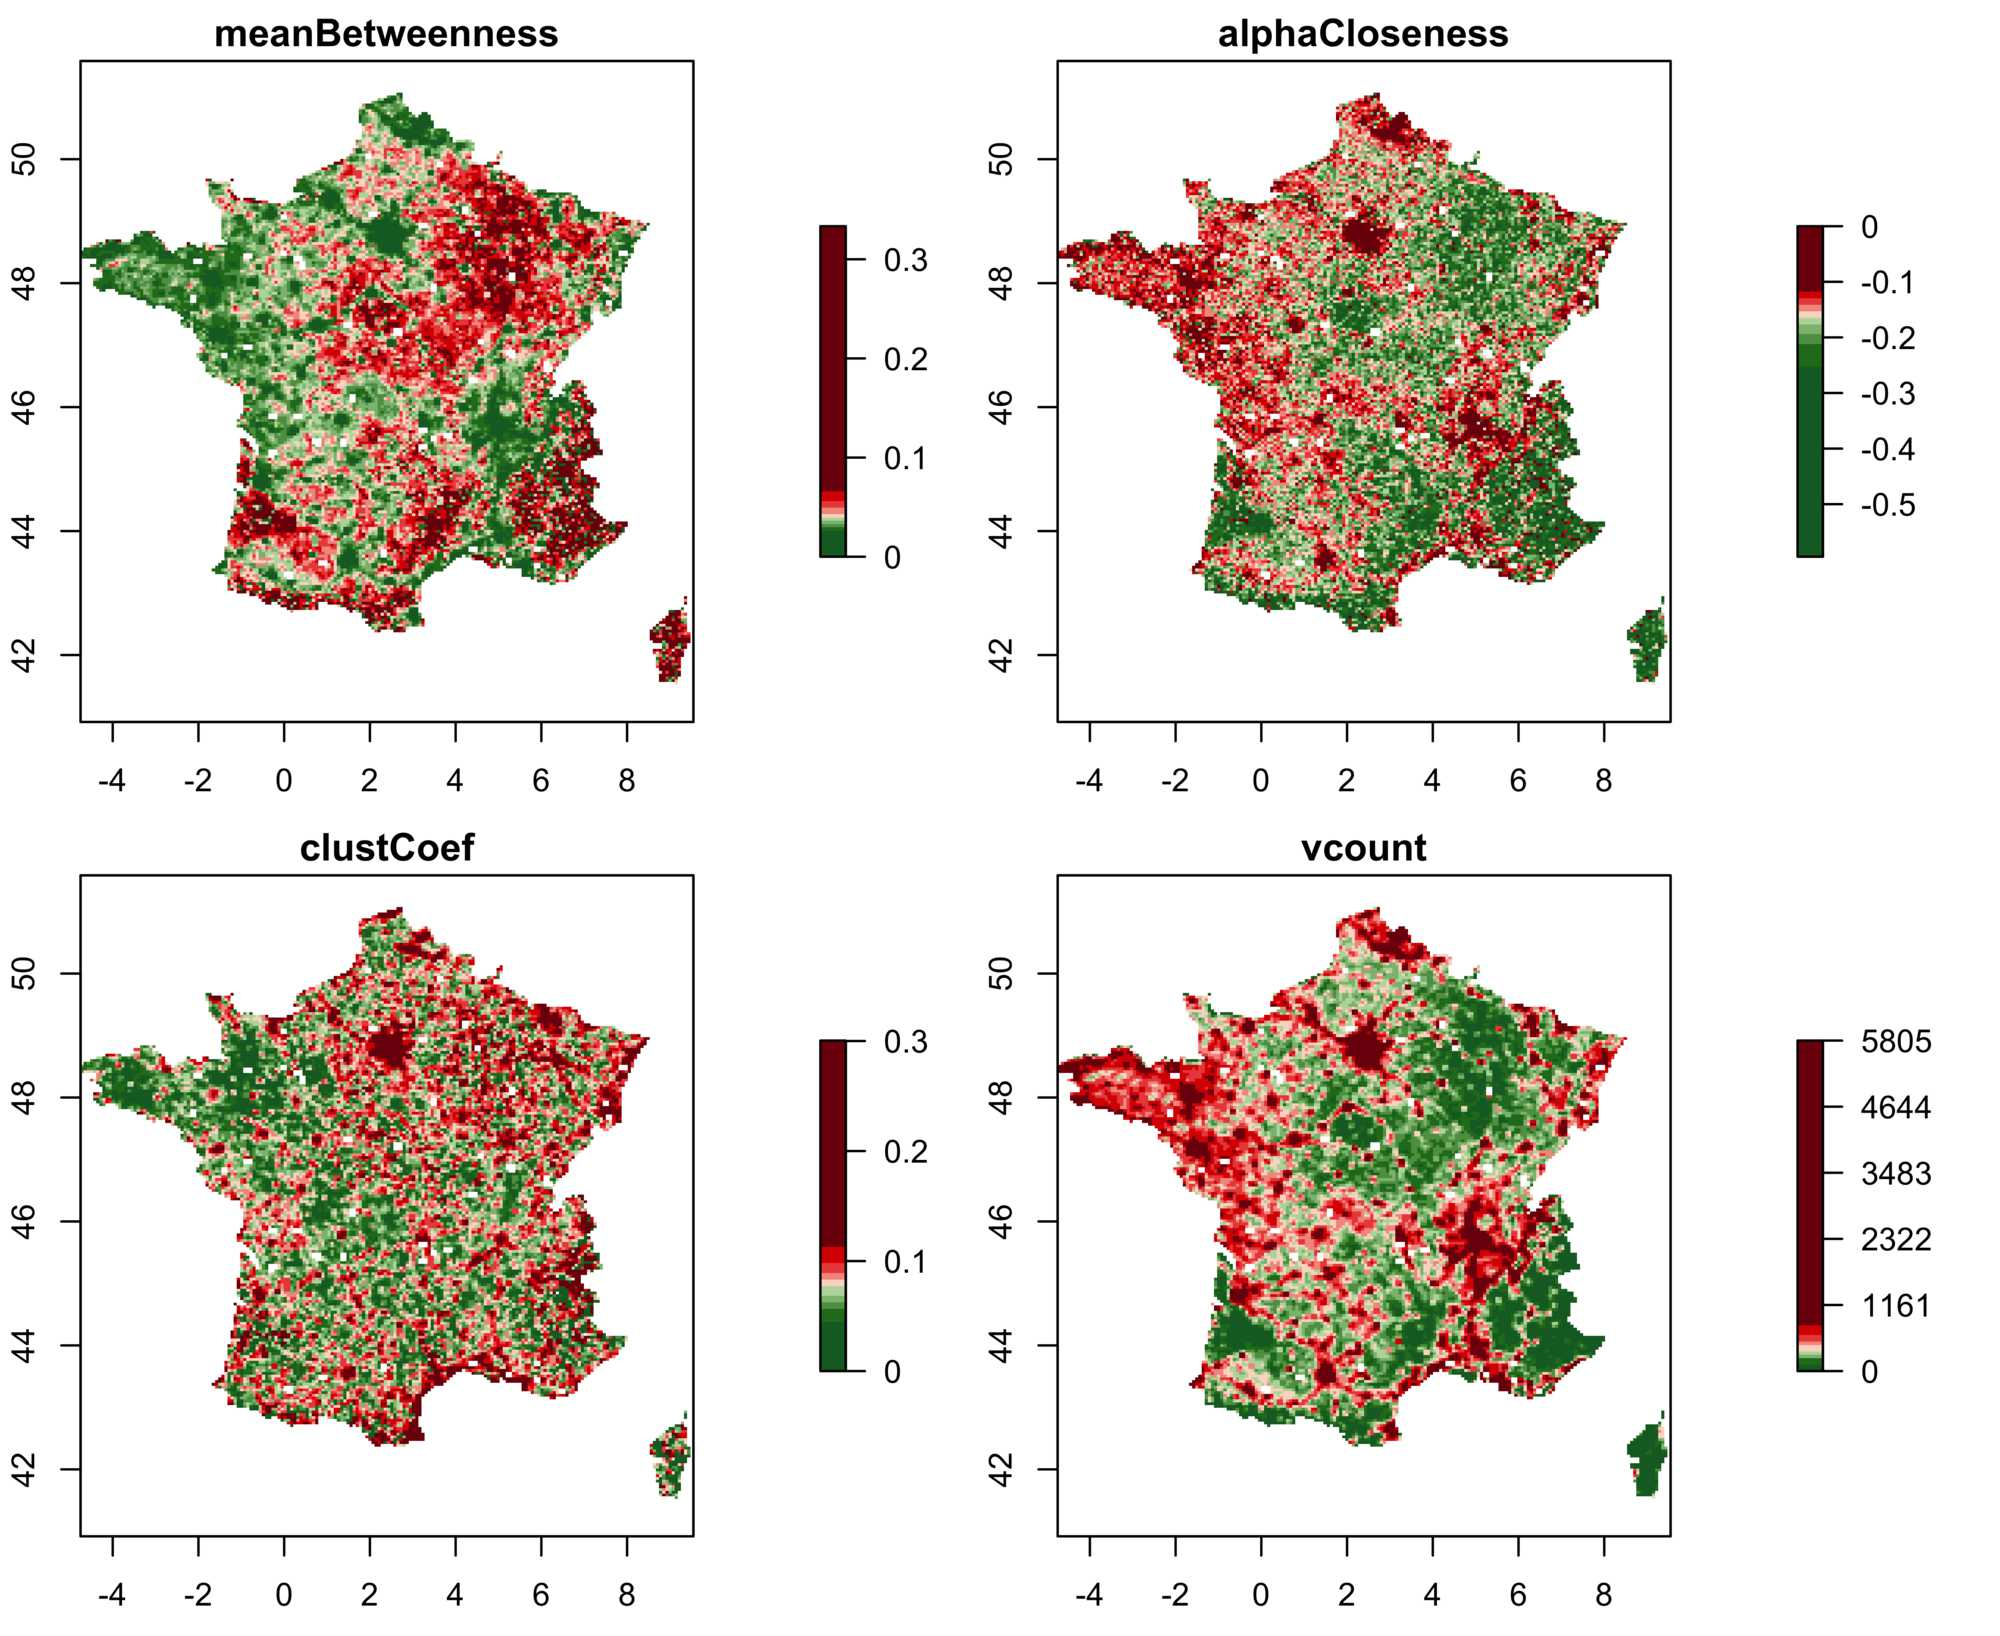
\includegraphics[width=\linewidth]{Figures/Final/4-1-2-fig-staticcorrs-network}
%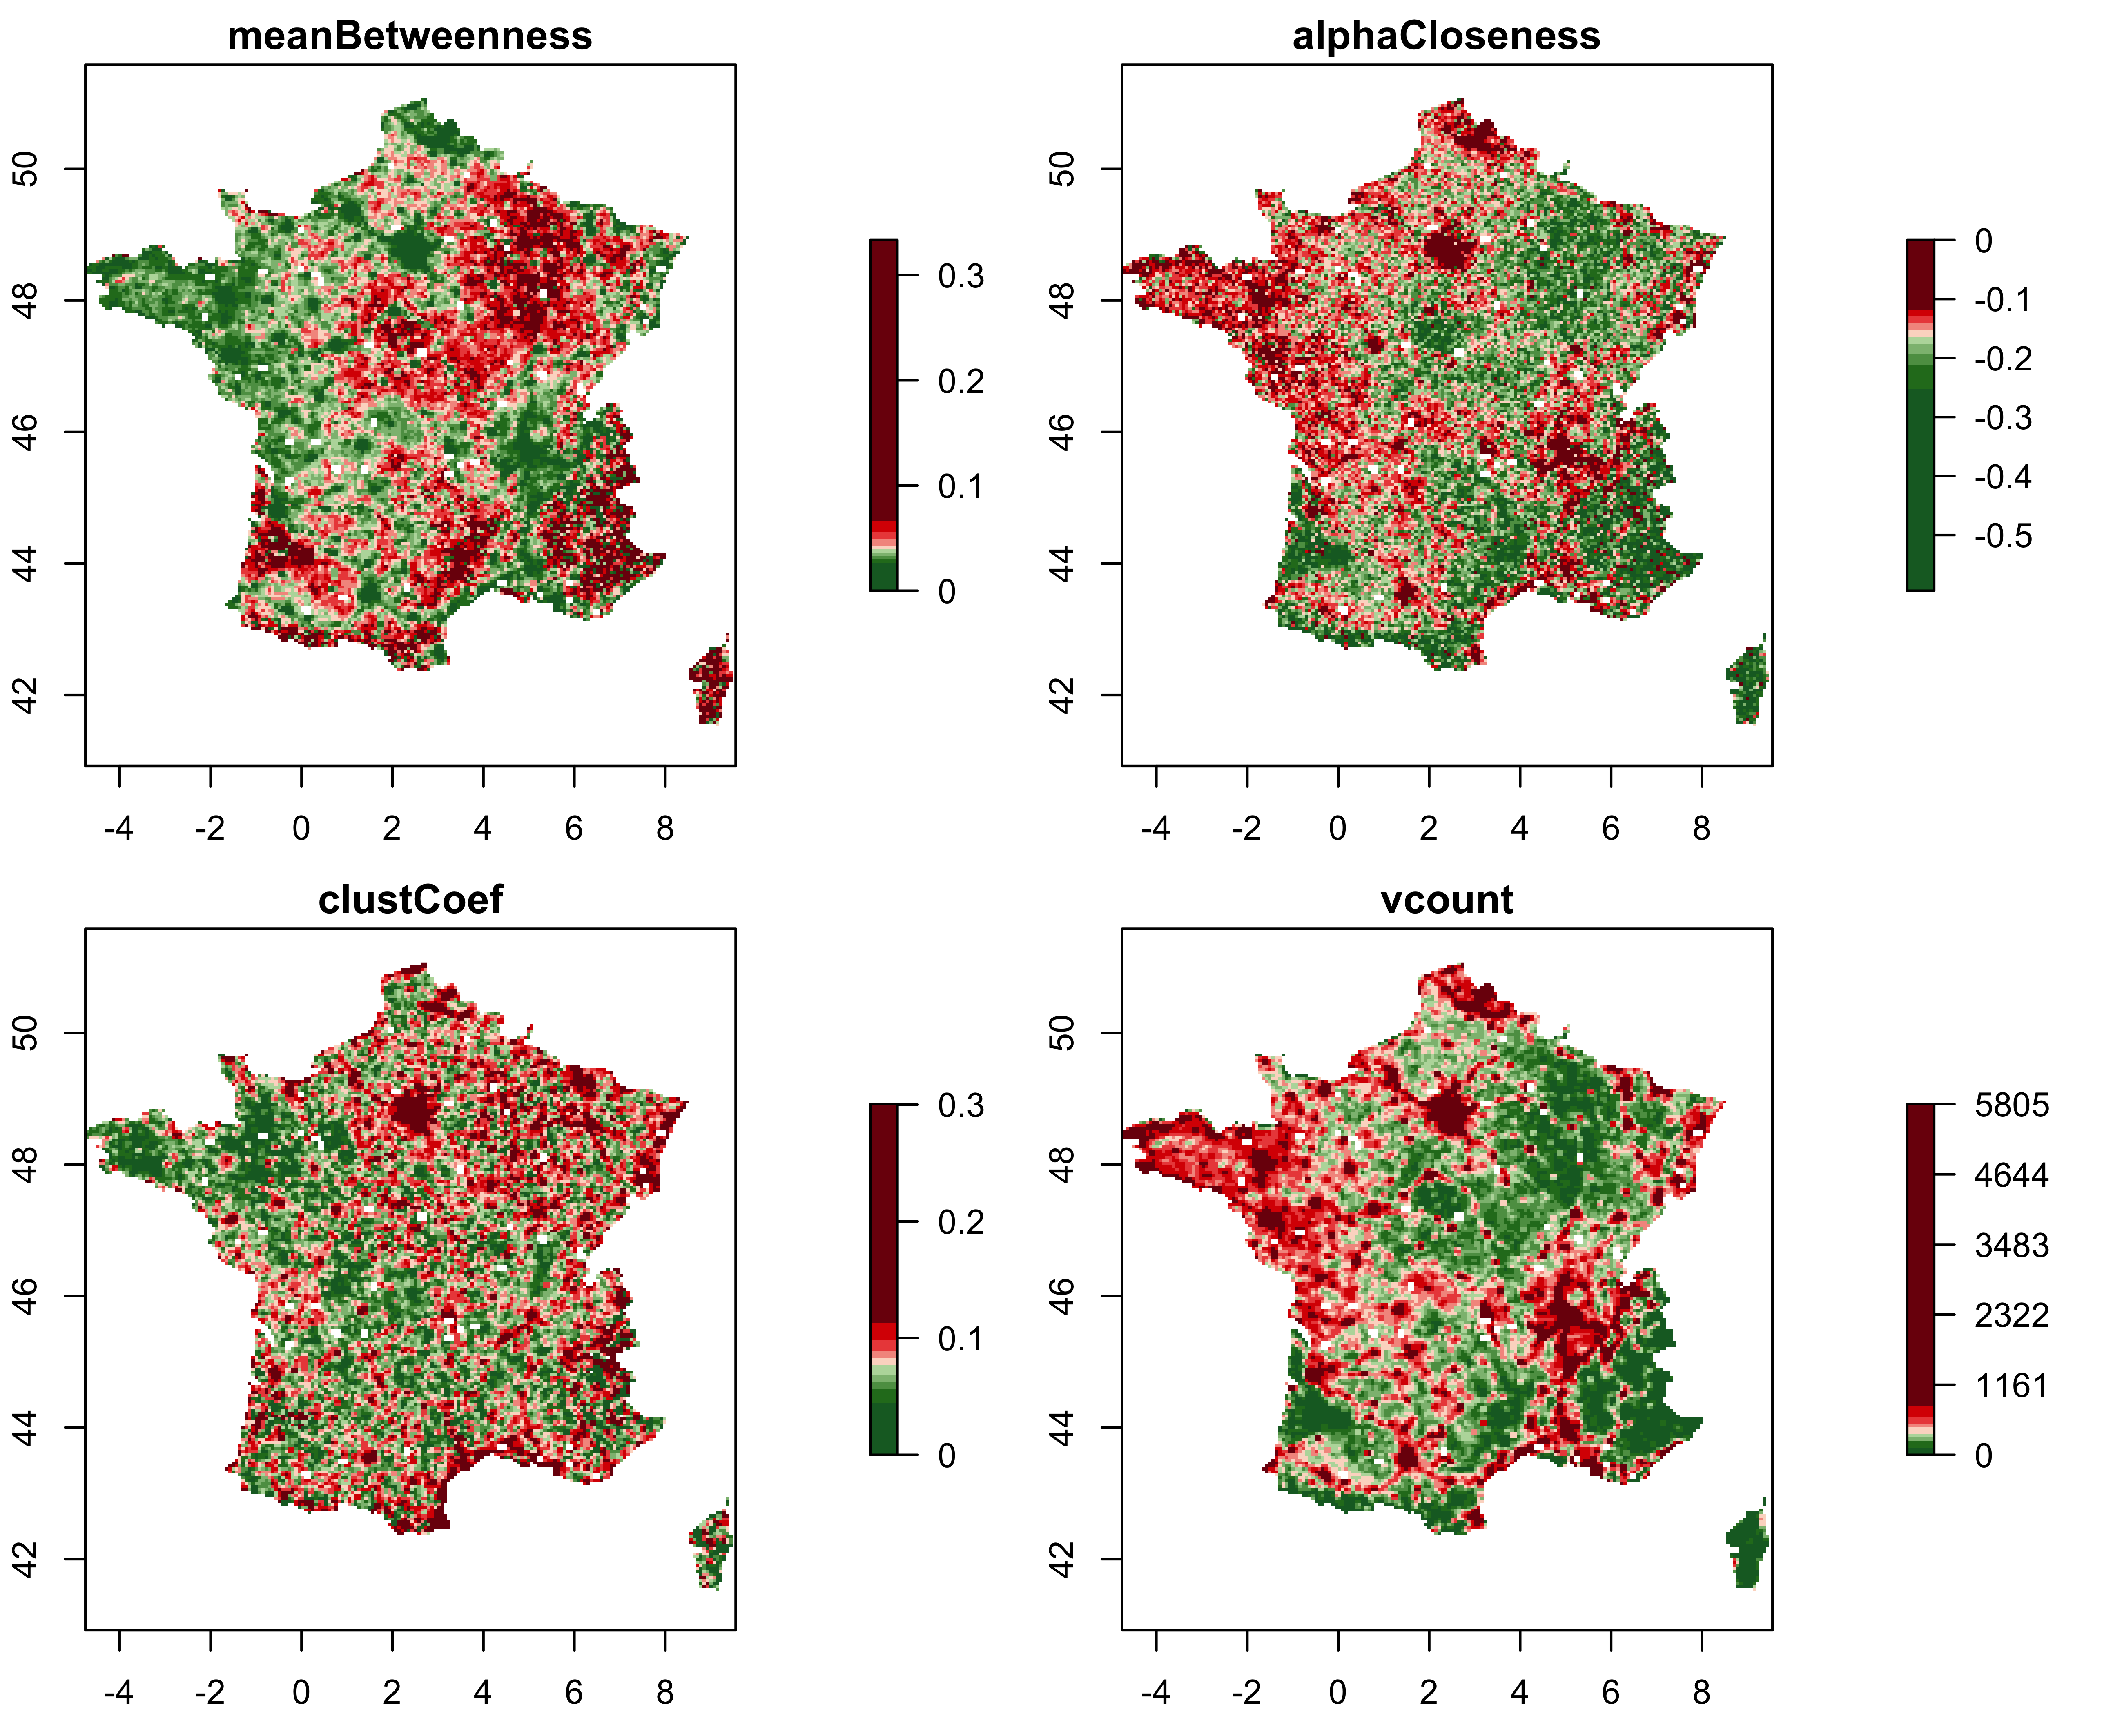
\includegraphics[width=\linewidth]{Figures/StaticCorrelations/FR_indics_network_selected_2_discrquantiles}
\caption[Empirical values of network indicators][Distribution spatiale des indicateur de réseau]{\textbf{Empirical values of network indicators.}\label{fig:staticcorrs:network}}{\textbf{Distribution spatiale des indicateur de réseau.} Nous donnons les indicateurs pour la France, en correspondance avec les indicateurs morphologiques décrits précédemment.\comment[FL]{faut-il garder les 4 ? traduire et expliquer}\label{fig:staticcorrs:network}}
\end{figure}
%%%%%%%%%%%%%%%%%%%%%%%%





%%%%%%%%%%%%%%%%%%
\subsection{Effective static correlations}{Correlations Statiques Effectives et Non-stationnarité}


%%%%%%%%%%%%%%%%%%
%\subsubsection{Correlations}{Corrélations}
% short overview of overall correlations and effective dimensions
% not really needed



%%%%%%%%%%%%%%%%%%
\paragraph{Spatial Correlations}{Corrélations spatiales}


\bpar{
Pour les correlations : zones de correlation pas trop grandes, carrés de base indicateurs plus petits : Computation of urban form indicators~\cite{le2015forme} and network indicators on $l_0=10km$ side square. Computation of spatial correlation on square areas of width $\delta\cdot l_0$ (with typically $\delta = 4, \ldots , 16$) We clearly unveil the local spatial stationarity of processes.
}{
Les corrélations spatiales locales sont calculées sur des fenêtres regroupant un certain nombre d'observation, et donc de fenêtres sur lesquelles les indicateurs ont été calculés. Notons $l_0$ (qui vaut 10km dans les résultats précédents) la résolution des distributions des indicateurs. L'estimation des corrélations s'effectue alors sur des carrés de taille $\delta\cdot l_0$ (avec $\delta$ pouvant varier typiquement de 4 à 16). La valeur de $\delta$ influe directement sur le nombre d'observations, et donc la fiabilité de l'estimation. Nous montrons en Figure~\ref{fig:staticcorrs:mapscorrs} des exemples de corrélations estimées avec $\delta = 12$ dans le cas de la France. Avec 29 indicateurs, la matrice de corrélation est assez conséquente en taille, mais la dimension effective est réduite : une analyse en composante principale montre que $p=10$ capture 60\% de la variance, et la première composante capture déjà 16\%, ce qui est considérable dans un espace où la dimension est de 406\footnote{Il s'agit de la dimension de la matrice de correlation entre 29 indicateurs, c'est à dire le nombre d'éléments de sa moitié moins sa diagonale.}.
}

\bpar{}{
On peut s'intéresser aux sous-blocs morphologique, de réseau, ou les corrélations croisées, qui exprime directement un lien entre les propriétés de la forme urbaine et celles du réseau. Par exemple, la relation entre Betweenness moyenne et hiérarchie morphologique que l'on visualise permet de comprendre la processus correspondant à la correspondance des hiérarchies : une population hiérarchisée peut induire un réseau hiérarchisé ou le sens inverse, mais elle peut également induire un réseau distribué ou celui-ci peut créer une hiérarchie de population - il faut bien comprendre en terme de correspondance et non de causalité, mais cette correspondance inform sur différents régimes urbains.
}

\bpar{}{
 Les métropoles semblent exhiber une corrélation positive dans ce cas, et des espaces ruraux négatifs. Cela suggère une très grande variété de régimes d'interaction. La variation spatiale de la première composante confirme celle-ci, ce qui révèle clairement la non-stationnarité spatiale des processus d'interaction entre formes, puisque les premiers et second moments varient dans l'espace. Nous donnons en Appendice~\ref{app:sec:staticcorrelations} d'autres exemples, pour l'ensemble de l'Europe et la Chine. Ces propriétés de non-stationnarité sont régulières pour l'ensemble de ces cas d'étude.\comment[FL]{difficile a suivre je decroche c'est dommage}
}



%%%%%%%%%%%%%%%%%%%%%%%%
\begin{figure}[h!]
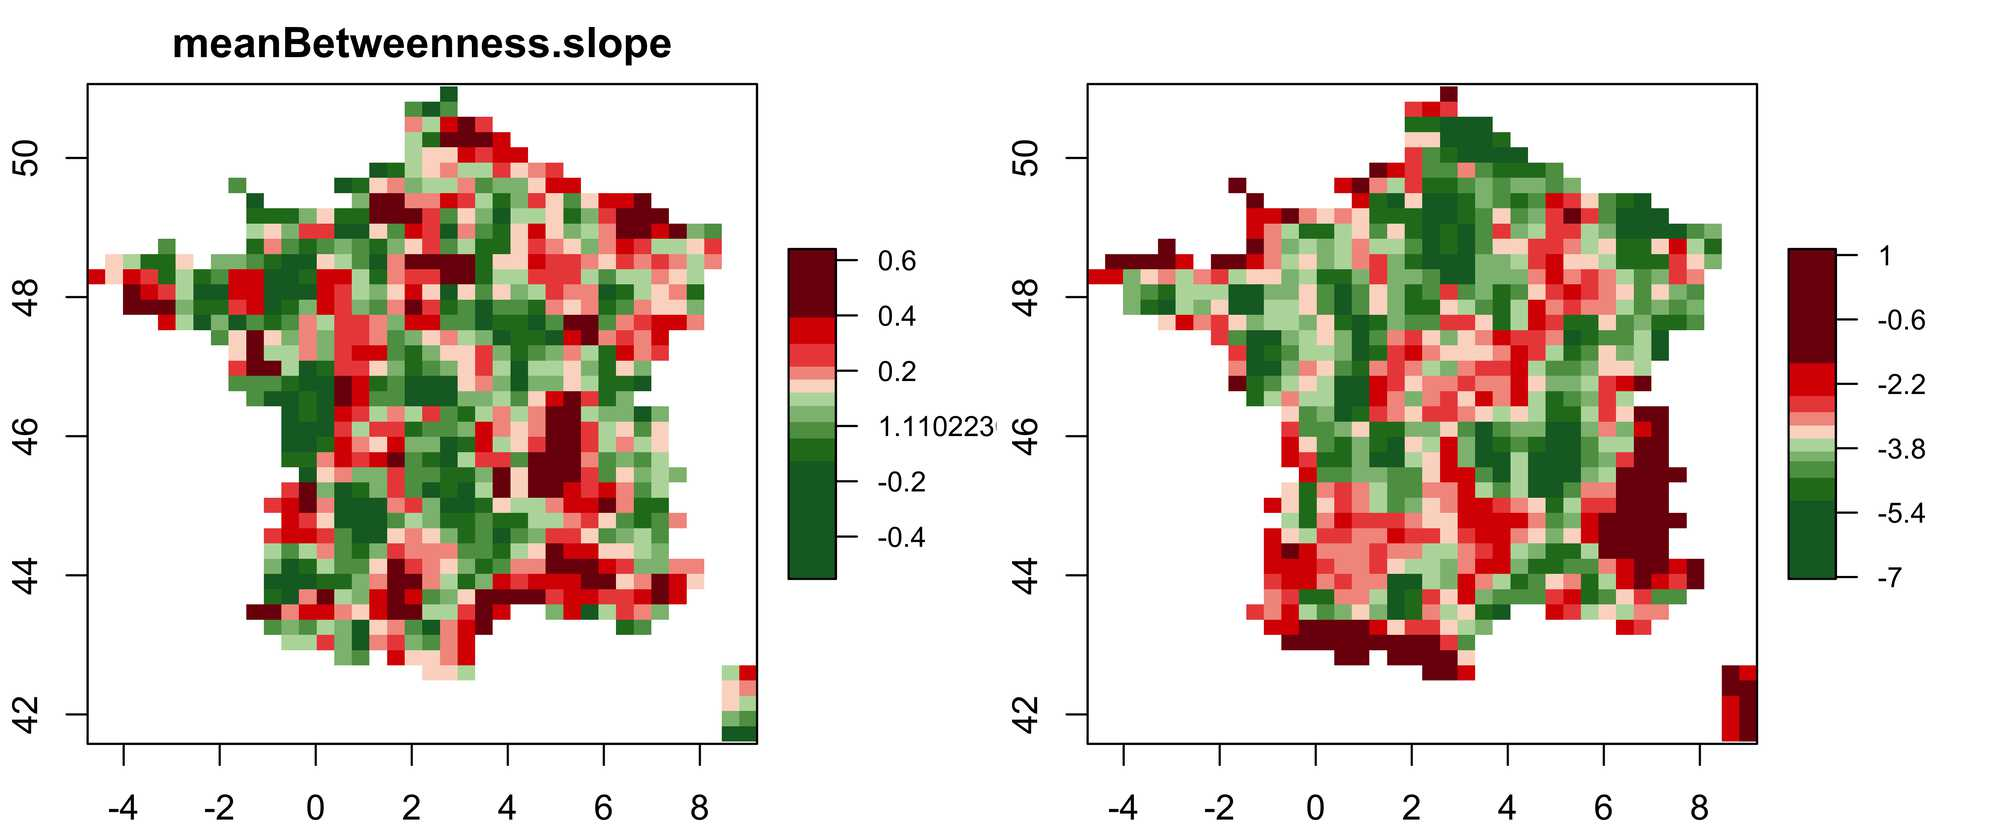
\includegraphics[width=\linewidth]{Figures/Final/4-1-3-fig-staticcorrs-mapscorrs}
%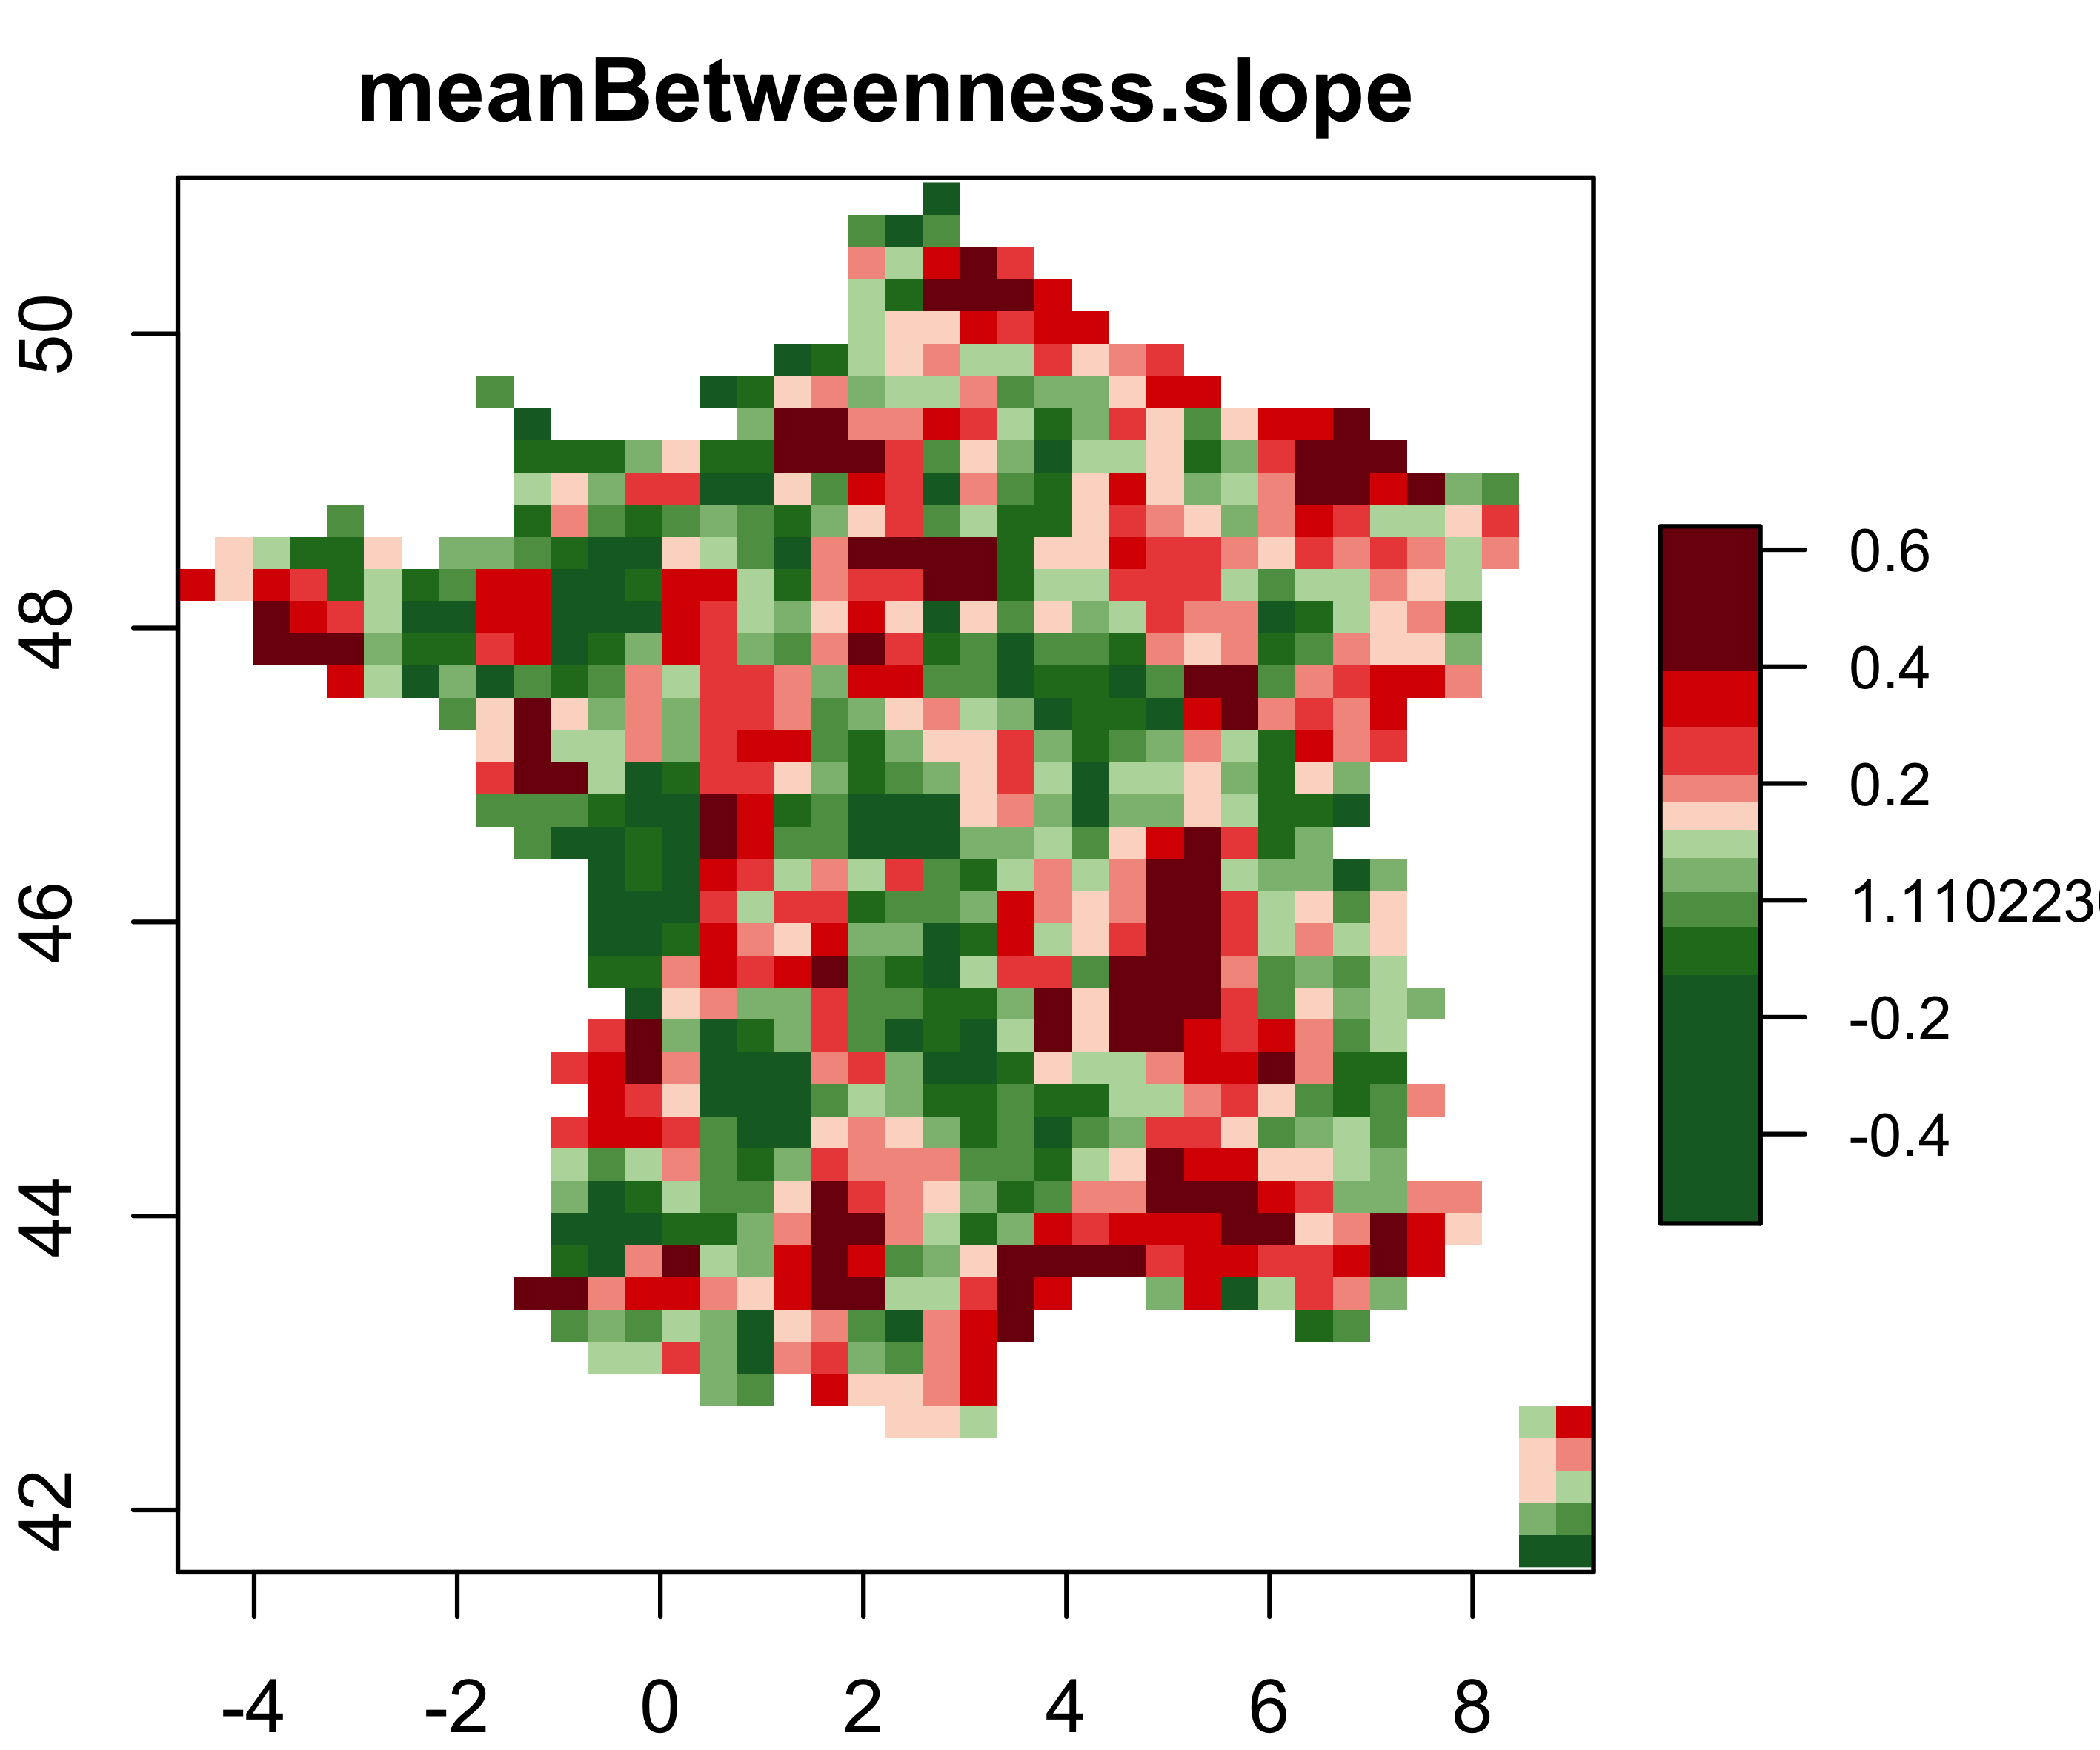
\includegraphics[width=0.48\linewidth]{Figures/StaticCorrelations/FR_corr_meanBetweenness_slope_rhoasize12}
%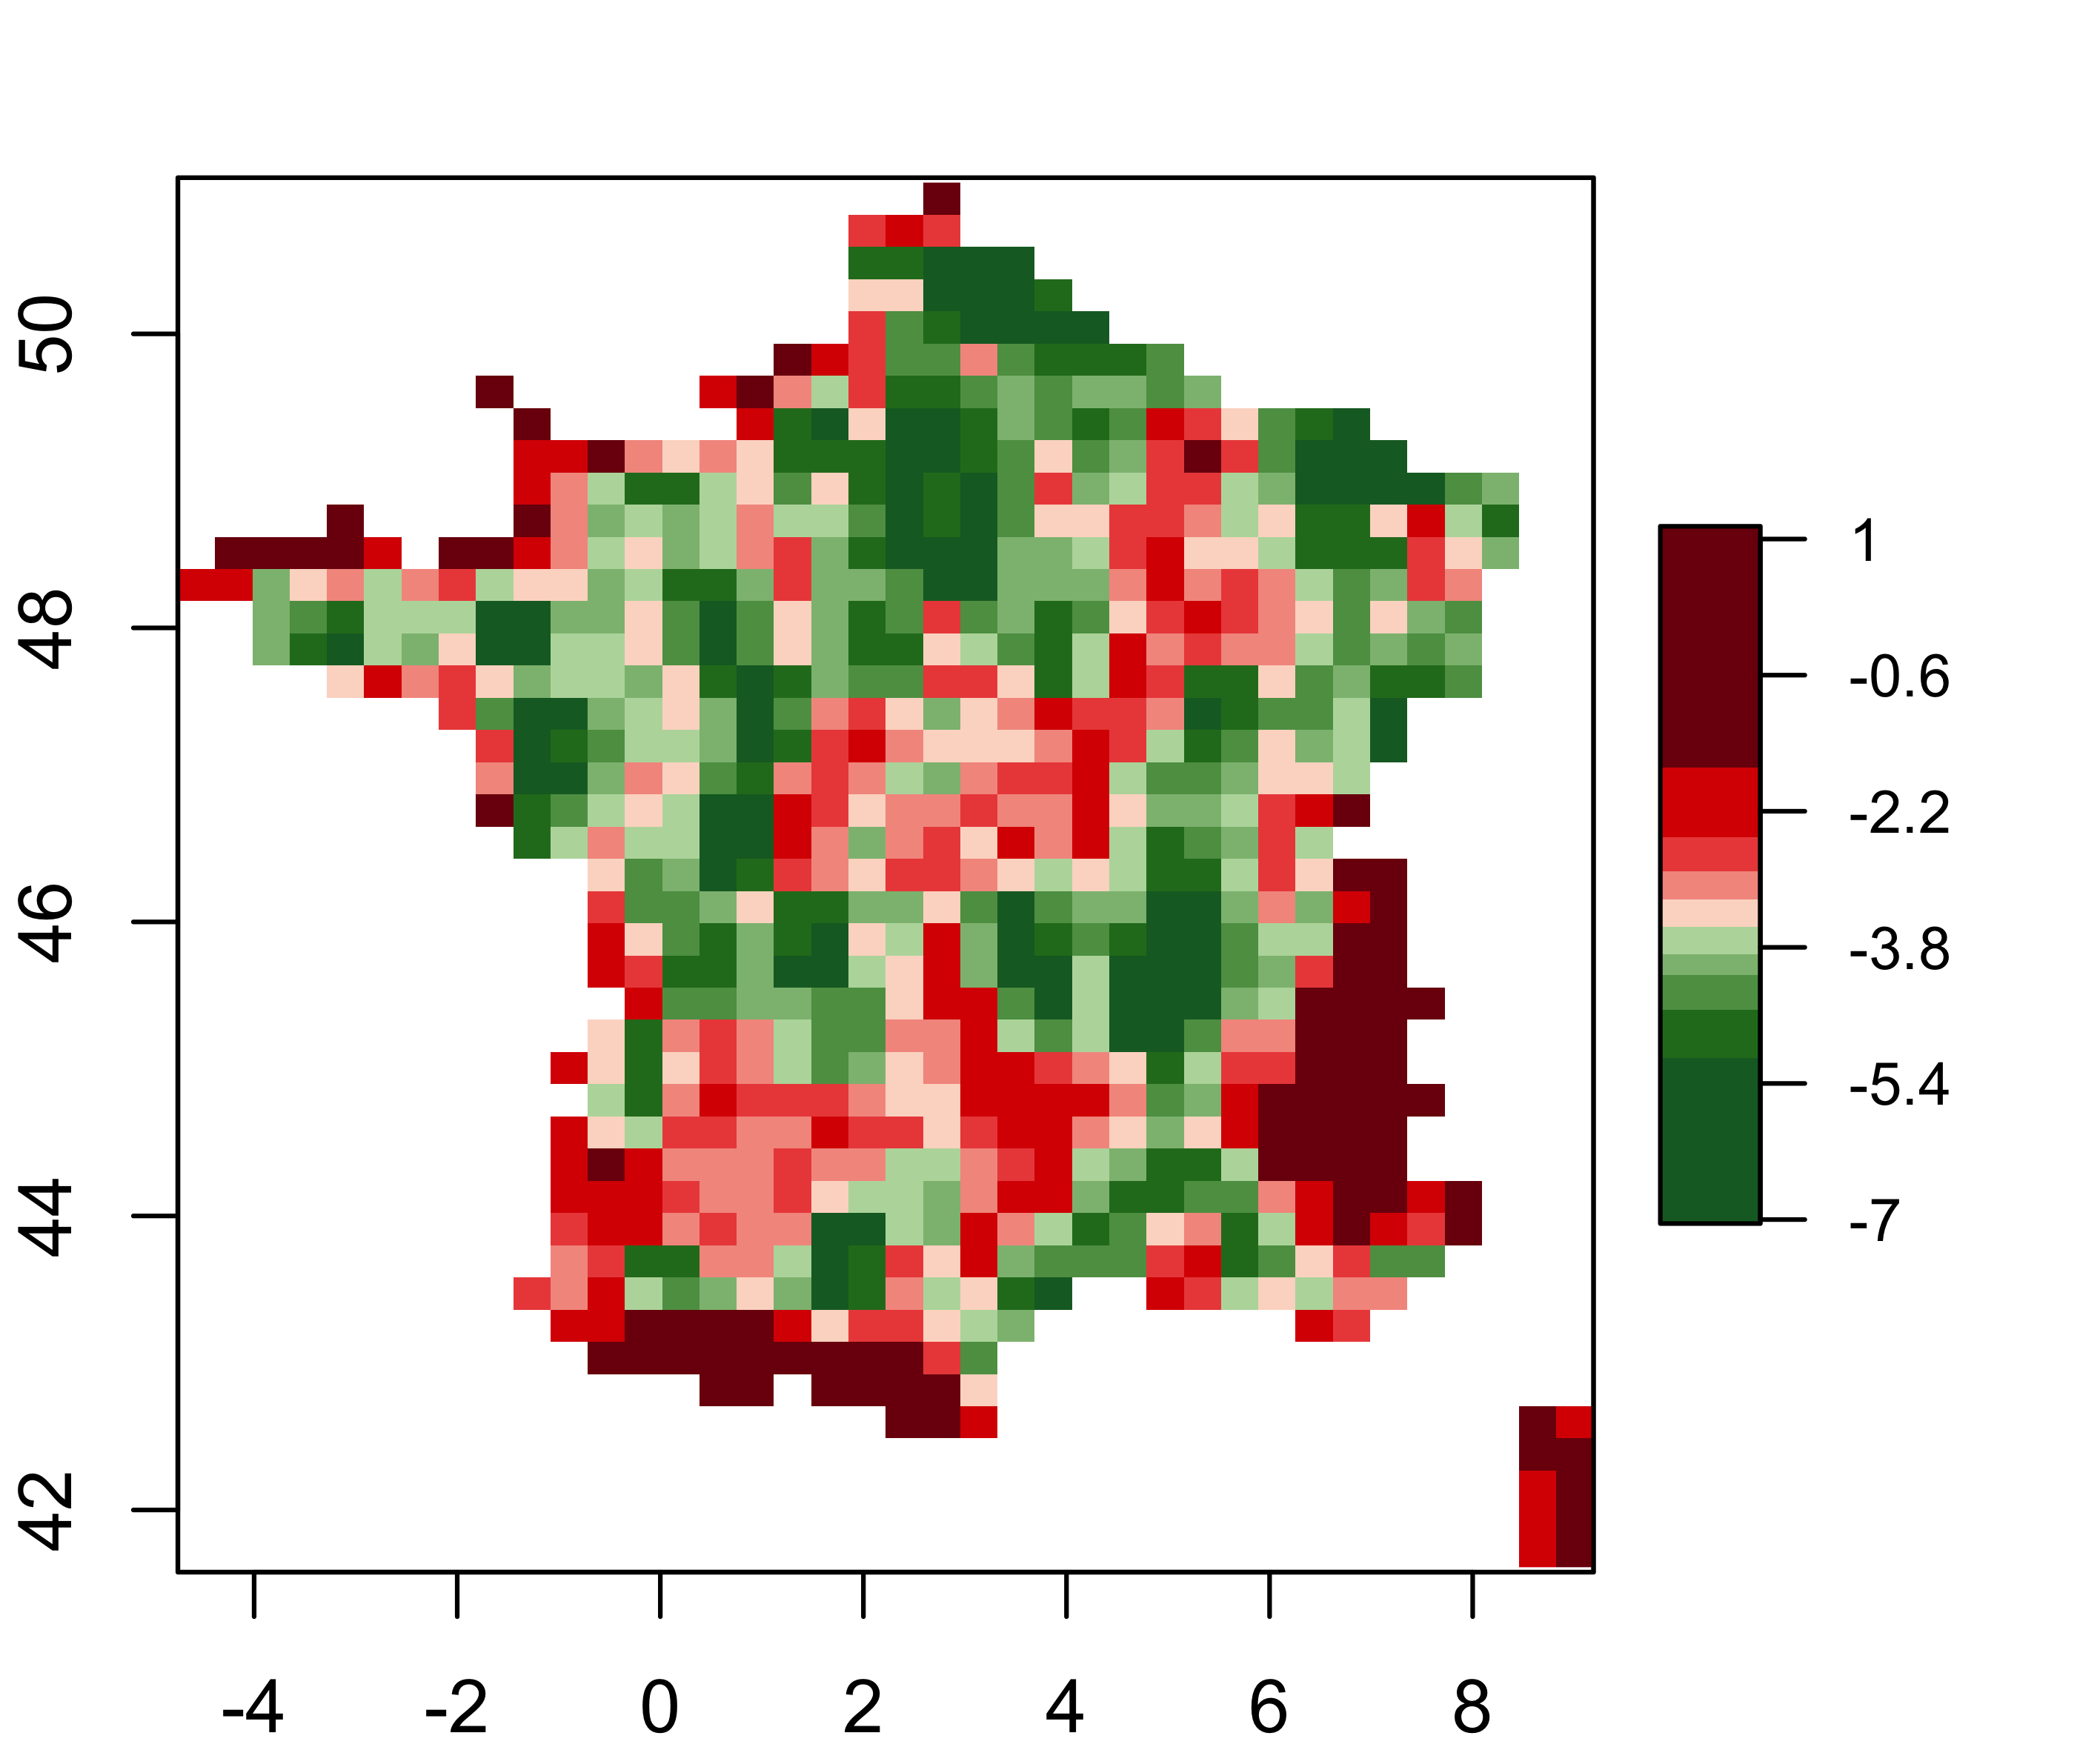
\includegraphics[width=0.48\linewidth]{Figures/StaticCorrelations/FR_corr_PCA_rhoasize12}
\caption[Spatial Correlations][Corrélations Spatiales]{Spatial Correlations\label{fig:staticcorrs:mapscorrs}}{\textbf{Exemples de corrélations Spatiales.} Pour la France, les cartes donnent $\rho\left[\bar{bw},\gamma\right]$ (gauche) et la première composante de la matrice réduite (droite).\label{fig:staticcorrs:mapscorrs}}
\end{figure}
%%%%%%%%%%%%%%%%%%%%%%%%



%%%%%%%%%%%%%%%%%%
\paragraph{Multi-scale Processes}{Nature multi-scalaire des processus}

\comment[FL]{mot delicat : est-ce une propriete intrinseque ? quelque chose que tu suggere ? etc. $\rightarrow$ revoir le titre.}[donner une def precise]

\comment[JR]{\cite{Chodrow31102017} : mesure des echelles intrinseques via theorie de l'info}

\bpar{
$\rightarrow$ Significant variation of mean correlation with $\delta$ (Left) and of normalized confidence interval (Right) given by $\left|\rho_+ - \rho_-\right|\cdot \delta$, as bounds theoretically vary as $\sqrt{N} \sim \sqrt{\delta^2}$ : implies multi-scalarity
}{
Nous montrons en Fig.~\ref{fig:staticcorrs:corrsdistrib} la variation de l'estimation des corrélations en fonction de la taille de la fenêtre. Plus précisément, on observe une forte variation (de plus de 0.1 pour chaque type) des correlations fonction de $\delta$, qui se reflète dans la valeur moyenne de la matrice. D'abord, la distribution statistique des corrélations suit une loi dont la forme s'apparente à celle d'une log-normale\comment[FL]{qu'est ce que c'est ? comment juges tu que c'est similaire ?}[tests ?] pour la morphologie seule, et plutôt normale pour le réseau et le croisement, ce qui voudrait dire que certaines zones ont des contraintes morphologiques assez fortes tandis que la forme du réseau est plutôt libre. On montre en Figure~\ref{fig:staticcorrs:corrsdistrib} ces distributions et les résultats des expériences de variation de $\delta$ pour l'Europe\comment[FL]{md}. On constate sur les nuages de points\comment[FL]{de la fig X} que les configurations où les corrélations croisées sont les plus fortes correspondent à celles où morphologique et réseau sont également fortes\comment[FL]{quest ce qui est fort dans cette phrase ? ce n'est pas comprehensible.}, confirmant l'imbrication des processus dans ce cas. L'augmentation de $\delta$ cause pour l'ensemble un décalage dans le positif, mais également un rétrécissement de la distribution, ces deux effets se traduisant par une décroissance des corrélations absolues moyennes, qui se stabilisent approximativement pour les grandes valeurs de $\delta$.\comment[FL]{quel apport thematique ?} Cette variation est révélatrice d'un comportement multi-échelle : le changement de la taille de la fenêtre ne devrait pas influer l'estimateur si un seul processus était sous-jacent, elle devrait seulement changer la robustesse de l'estimation.\comment[FL]{c'est une affirmation a justifier !!}
}


\bpar{}{
La variation de la taille de l'intervalle de confiance normalisée, qui en théorie sous hypothèse de normalité devrait conduire $\delta\cdot \left|\rho_+ - \rho -\right|$ à être constant, puisque les bornes varient asymptotiquement comme $1/\sqrt{N}\sim 1/\sqrt{\delta^2}$ (la démonstration est donnée en Appendice~\ref{app:sec:staticcorrelations}). Cela confirme bien cette première hypothèse.
}



Ainsi, les processus sont à la fois non-stationnaires et multi-scalaires.\comment[FL]{je trouve que le statut de la preuve est maigre et qu'en tout cas tu n'explicite pas clairement cela}


%%%%%%%%%%%%%%%%%%%%%%%%
\begin{figure}
%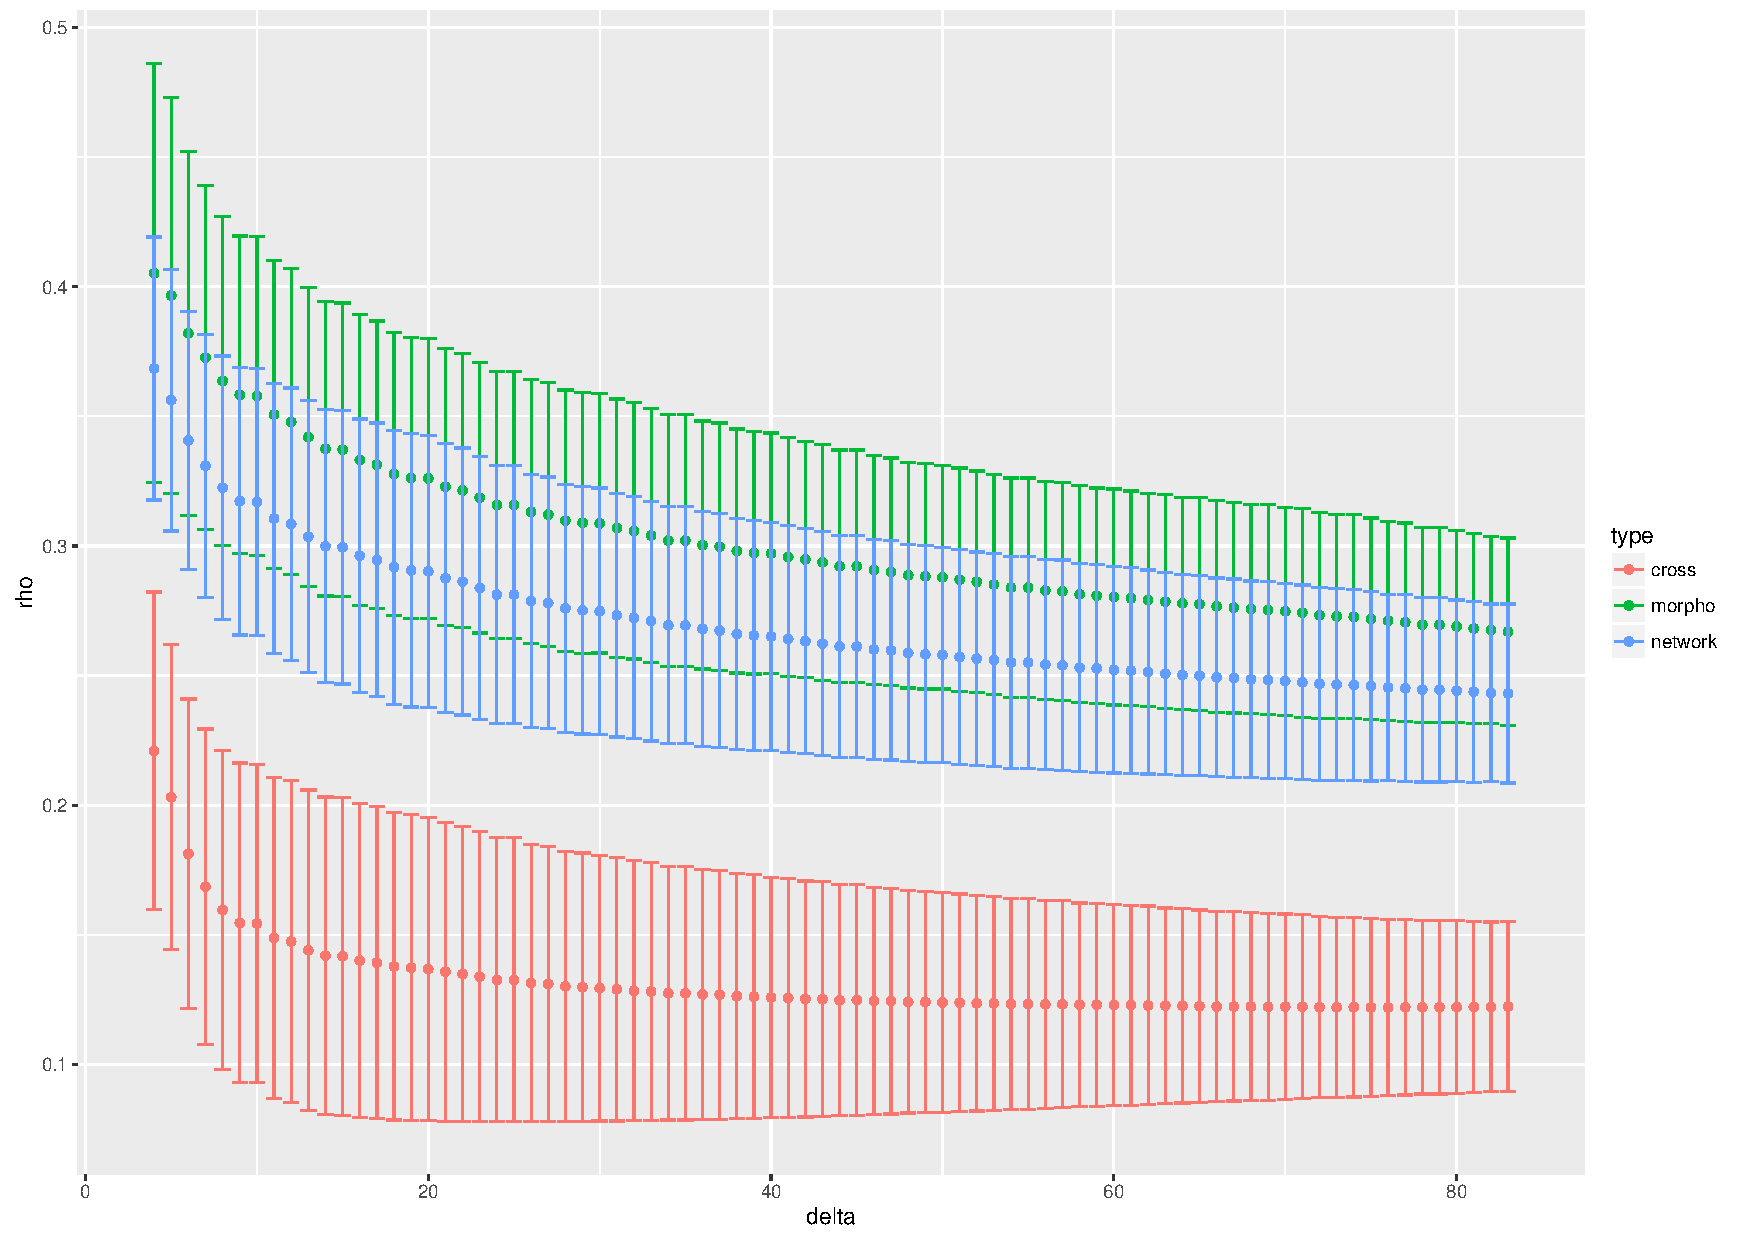
\includegraphics[width=0.48\linewidth]{Figures/StaticCorrelations/corrs-summary-meanabs_varyingdelta_bytype}\\
%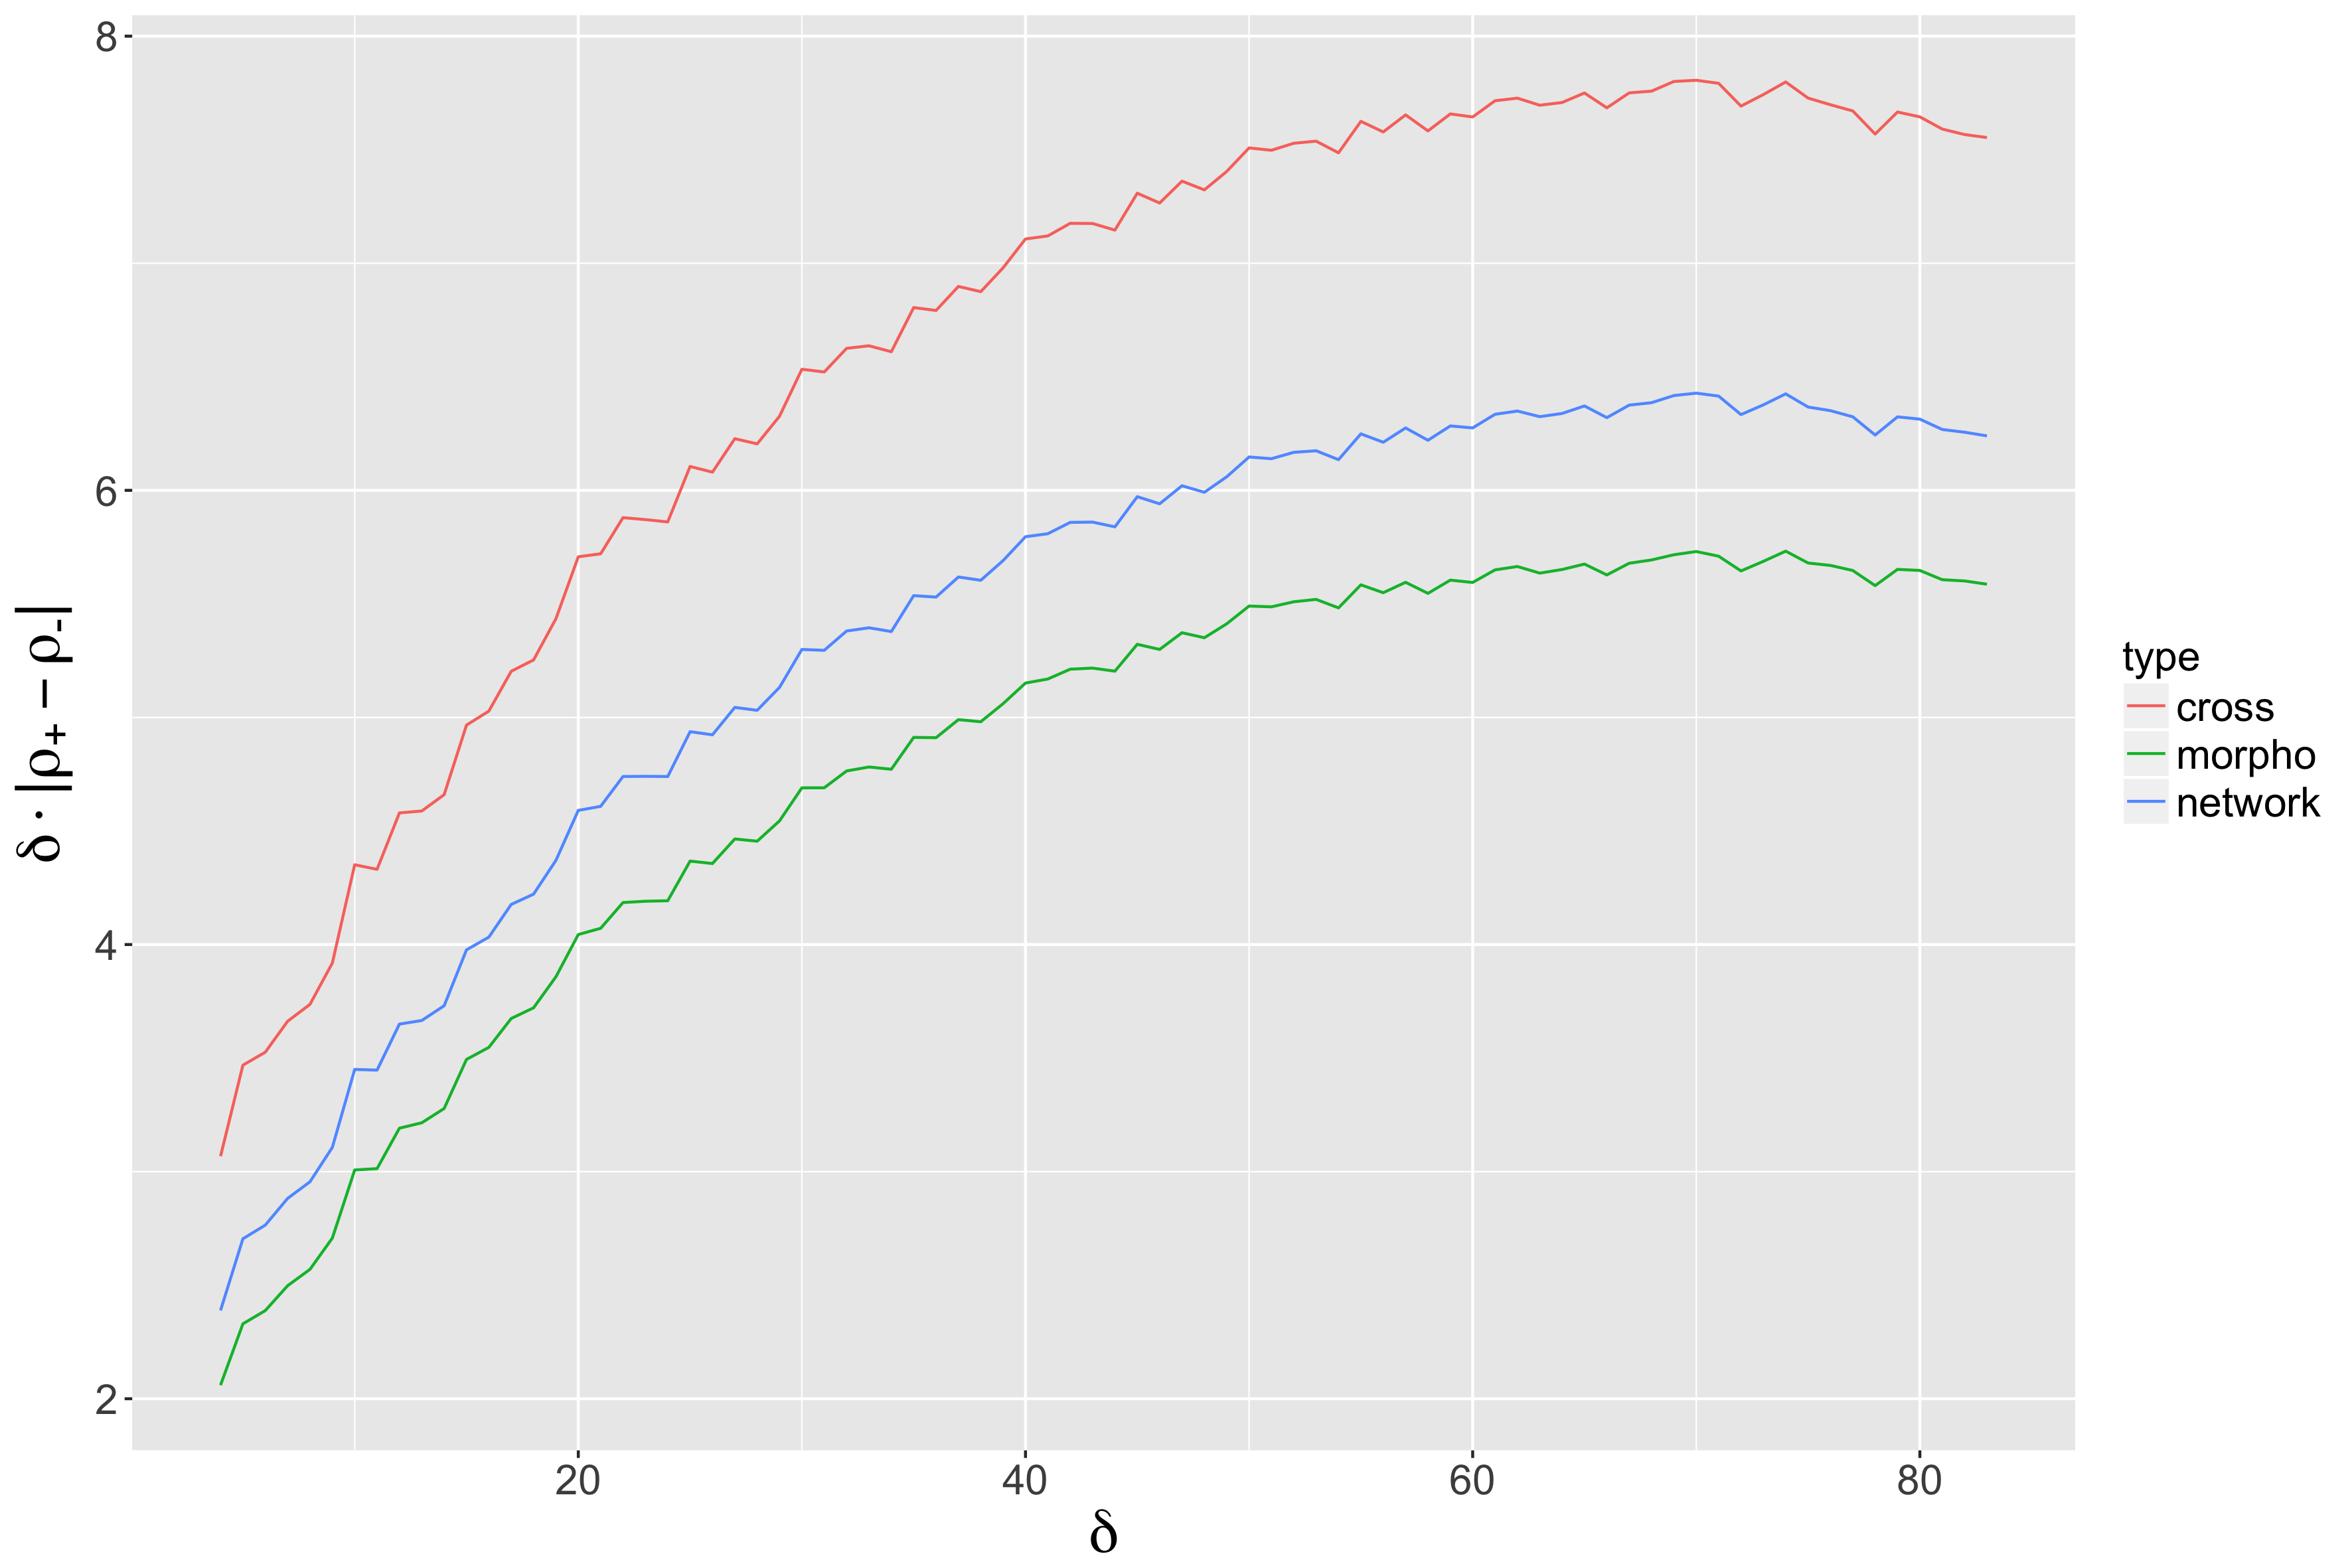
\includegraphics[width=0.48\linewidth]{Figures/StaticCorrelations/normalized_CI_delta}
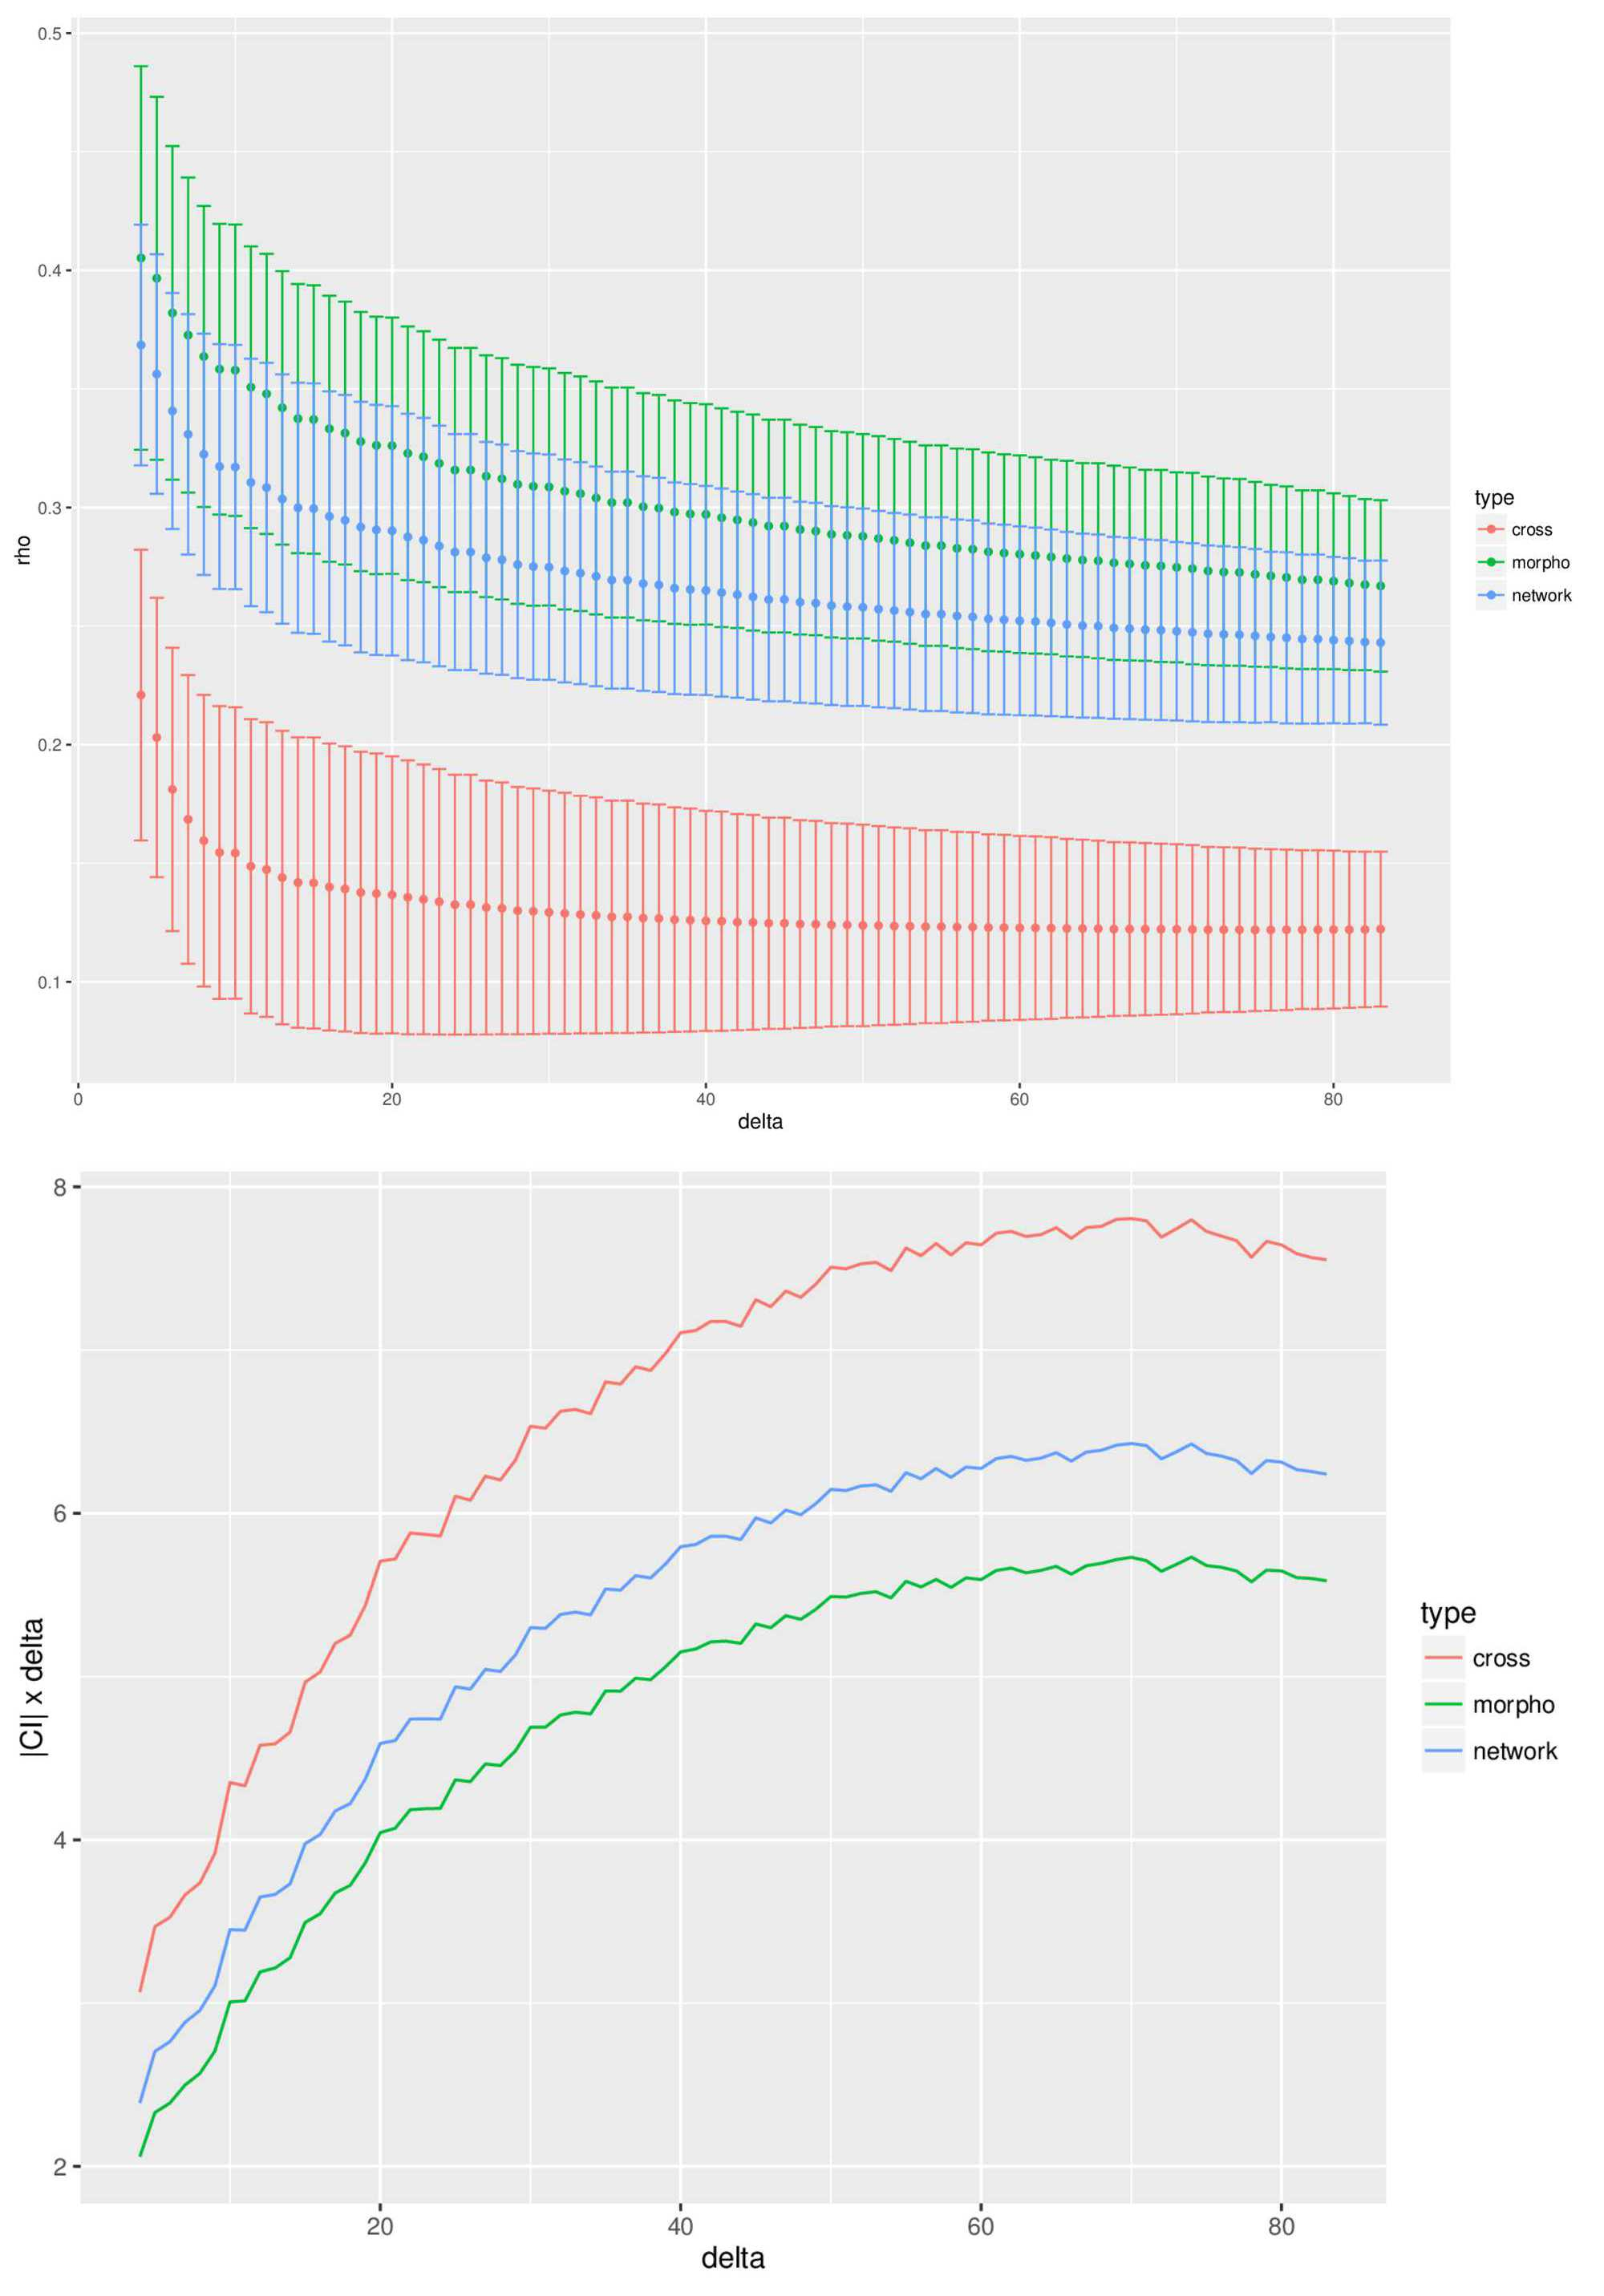
\includegraphics[width=\linewidth,height=0.85\textheight]{Figures/Final/4-1-3-fig-staticcorrs-corrsdistrib}
\caption[Variation of correlations with scale][Variation des corrélations avec l'échelle]{\textbf{Variation of correlations with scale.}\label{fig:staticcorrs:corrsdistrib}}{\textbf{Variation des corrélations avec l'échelle, pour les corrélations calculées sur l'Europe.} \textit{(Haut)} Correlations absolues moyennes et leur déviation standard, pour les différents blocs, en fonction de $\delta$ ; \textit{(Bas)} Taille de l'intervalle de confiance normalisée $\delta\cdot \left|\rho_+ - \rho -\right|$ (IC estimé par méthode de Fisher) en fonction de $\delta$ \label{fig:staticcorrs:corrsdistrib}}
\end{figure}
%%%%%%%%%%%%%%%%%%%%%%%%



%%%%%%%%%%%%%%%%%%
\paragraph{Optimal Scales}{Echelles optimales}


\bpar{
We also compute the optimal bandwidth for a GWR PCA~\cite{harris2011geographically}. We beware to sample data accordingly to avoid local colinearity :\cite{wheeler2007diagnostic} colinearity in GWR
}{
Nous explorons d'autre part la propriété de multi-scalarité par extraction d'échelles endogène présentes dans les données. Une Analyse en Composantes Principales Géographique Pondérée (GWRPCA)~\cite{harris2011geographically} suggère des poids et importances variables dans l'espace, ce qui est cohérent avec la non-stationnarité des structures de corrélation obtenue ci-dessus. Il n'y a a priori pas de raison pour que les échelles de variation des différents indicateurs soient strictement identiques. Nous proposons donc d'extraire les échelles typiques pour les relations croisées entre forme urbaine et forme de réseau.
}


\bpar{}{
Nous implémentons pour cela la méthode suivante : nous considérons un échantillon typique d'indicateurs (quatre pour chaque aspect), et pour chaque indicateur nous formulons l'ensemble des modèles linéaires possibles en fonction des indicateurs opposés (réseau pour un indicateur morphologique, morphologique pour un indicateur de réseau), visant à capturer directement l'interaction sans contrôle sur le type de forme ou de réseau. Ces modèles sont alors ajustés par une Régression Géographique Pondérée (GWR) à portée optimale déterminée par critère d'information corrigé (AICc). Pour chaque indicateur, on retient le modèle ayant la meilleure valeur du critère d'information. Nous ajustons les modèles sur les données de la France, avec un noyau \emph{bisquare} et une portée adaptable en nombre de voisins.
}

\bpar{}{
Les résultats sont présentés en Table~\ref{tab:staticcorrelations:gwr}. Il est intéressant de noter dans un premier temps que l'ensemble des modèles ne comprend qu'une seule variable, suggérant des correspondances relativement directes entre topologie et morphologie. L'ensemble des indicateurs morphologiques est expliqué par la performance du réseau, c'est à dire la quantité de détour qu'il comprend. Au contraire, la topologie est expliquée par le Moran pour les centralités, et par l'entropie pour la performance et le nombre de sommets. On a ainsi une dissymétrie des relations, le réseau étant conditionné de manière plus complexe à la morphologie que la morphologie au réseau. Les ajustements sont bons ($R^2 > 0.5$) pour une majorité d'indicateurs. Les échelles optimales sont quant à elles très localisées, de l'ordre de la dizaine de kilomètres, c'est à dire une plus grande variation que celle obtenue par les corrélations.
}

%bestmodels
%            indic             bestmodel      dist    bw        R2
%           <fctr>                <fctr>     <dbl> <dbl>     <dbl>
%1        distance  distance~networkPerf 11.609078    30 0.3145114
%2         entropy   entropy~networkPerf  8.795393    16 0.7511295
%3 meanBetweenness meanBetweenness~moran 12.294076    34 0.5776019
%4   meanCloseness   meanCloseness~moran 13.883025    44 0.2565047
%5           moran     moran~networkPerf  8.795393    16 0.4886164
%6     networkPerf   networkPerf~entropy  8.595512    15 0.8640510
%7           slope     slope~networkPerf  8.795393    16 0.6840567
%8          vcount        vcount~entropy  8.595512    15 0.8825783


%%%%%%%%%%%%%%%%%%
\begin{table}
\caption[][Relation croisées entre indicateurs de réseau et morphologiques]{}{\textbf{Relation croisées entre indicateurs de réseau et morphologiques.} Chaque relation est ajustée par une Regression Géographique Pondérée, pour la portée optimale ajustée par AICc.\label{tab:staticcorrelations:gwr}}
\begin{tabular}{|l|l|l|l|}
\hline
Indicateur & Modèle & Portée & Fit (R2) \\ \hline
distance & distance $\sim$ networkPerf & 11.609078 & 0.3145114 \\
entropy  & entropy $\sim$ networkPerf &  8.795393  &0.7511295 \\
meanBetweenness & meanBetweenness $\sim$ moran & 12.294076 & 0.5776019 \\
meanCloseness &  meanCloseness $\sim$ moran & 13.883025 & 0.2565047 \\
moran & moran $\sim$ networkPerf &  8.795393 & 0.4886164 \\
networkPerf & networkPerf $\sim$entropy & 8.595512  & 0.8640510 \\
slope & slope $\sim$ networkPerf & 8.795393  & 0.6840567 \\
vcount & vcount $\sim$ entropy & 8.595512  & 0.8825783 \\\hline
\end{tabular}
\end{table}
%%%%%%%%%%%%%%%%%%



%%%%%%%%%%%%%%%%%%
\subsubsection{Spatial non-stationarity and non-ergodicity}{Non-stationnarité spatiale et non-ergodicité}


\paragraph{Formalization}{Formalisation}

\bpar{
We propose to formalize our empirical findings. Let $Y_i\left[\vec{x},t\right]$ a spatio-temporal stochastic process. We showed following assumptions:
\begin{enumerate}
\item Local spatial autocorrelation is present and bounded by $l_{\rho}$ (in other words the processes are continuous in space) : at any $\vec{x}$ and $t$, $\left|\rho_{\norm{\Delta \vec{x}} < l_{\rho}}\left[Y_i (\vec{x}+\Delta \vec{x},t), Y_i (\vec{x},t) \right]\right| > 0$.
\medskip
\item Processes are locally parametrized : $Y_i = Y_i\left[\alpha_i\right]$, where $\alpha_i (\vec{x})$ varies with $l_{\alpha}$, with $l_{\alpha} \gg l_{\rho}$ and weakly locally stationary in space.
\medskip
%\item Spatial correlations between processes have a sense at an intermediate scale $l$ such that $l_{\alpha}\gg l \gg l_{\rho}$.
%\item Processes covariance stationarity times scale as $\sqrt{l}$.
%\item Local ergodicity is present at scale $l$ and dynamics are locally chaotic.
\item Processes are multi-scalar : since $\rho(\delta = \infty) > \rho (\delta = 0 )$, a necessary non-linear correction on processes spatial averages in correlation computation is present.
% add computation in supplementary materials / papers. -> later
\end{enumerate}
}{
Formalisons les conclusions empiriques obtenues. Soit $Y_i\left[\vec{x},t\right]$\comment[FL]{?} un processus stochastique\comment[FL]{faut-il que ce soit generique ? le dire alors} spatio-temporel. Nous avons alors les hypothèses suivantes :
\begin{enumerate}
\item L'autocorrelation spatiale locale existe en dessous d'une échelle minimale $l_0$ (en d'autres termes le processus est continu dans l'espace) : pour tout $\vec{x}$ et $t$, on a $\left|\rho_{\norm{\Delta \vec{x}} < l_0}\left[Y_i (\vec{x}+\Delta \vec{x},t), Y_i (\vec{x},t) \right]\right| \neq 0$.
\item Les processus sont localement paramétrés\comment[FL]{?} : $Y_i = Y_i\left[\alpha_i\right]$, où $\alpha_i (\vec{x})$ varie à l'échelle $l_{\alpha}$, avec $l_{\alpha} \gg l_0$ et est localement stationnaire\comment[FL]{sens ?} dans l'espace.
\item Les processus sont multi-scalaires\comment[FL]{def} : comme $\rho(\delta = \infty) > \rho (\delta = 0 )$\comment[FL]{aucun sens}, une nécessaire correction non-linéaire sur les moyennes spatiales des processus est présente dans le calcul des corrélations.\comment[FL]{c'est hyperflou et donc non-reproductible}
\end{enumerate}
}

\comment[FL]{qu'est ce que cela veut dire pour toi, multi scalaire ?}


\paragraph{On global non-ergodicity}{Sur la non-ergodicité globale}

\bpar{
Analytical Deductions
1. \textbf{Regimes of temporal correlations.} Let assume local ergodicity in $\vec{x}_0$ at scale $\delta \cdot l_0$ (reasonable with urban growth and network extension in recent times). The Ergodic theorem implies that $\exists \mathcal{T}$ such that

\[<Y_i (t) >_{\norm{\vec{x}-\vec{x}_0} < \delta\cdot l_0} = <Y_i (\vec{x}_0)>_{t\in \mathcal{T}}\] 

With spatial stationarity, $<Y_i>_{\vec{x}_0}=<Y_i>_{\vec{x}_1}$, thus $\mathcal{T}$ must be constant to be invariant by translation. By contraposition and (2), processes have different dynamical characteristics.
% if translate in a given direction, looses a small part, must be compensated by the area translated by delta (overlap), thus must be constant.
}{
Nous proposons d'établir un lien entre les propriétés de non-stationnarité et la non-ergodicité globale des systèmes. Nous rappelons qu'il s'agit d'un aspect essentiel postulé par la Théorie Evolutive~\cite{pumain2012urban}, conduisant à discuter les interprétation universelles des systèmes urbains proposées par les théories du Scaling~\cite{bettencourt2007growth}. Nous suggérons que la non-stationnarité spatiale est reliée d'une part à différentes échelles de temps impliquées, et d'autre part à une non-ergodicité globale\comment[FL]{le lecteur ne te suit plus : c'est trop rapide}, sous l'hypothèse de stationnarité et d'ergodicité locale. Cette dernière parait raisonnable, au sens ou un régime local se manifestera de manière aléatoire sur ses différentes instances locales dans le cas d'indicateurs effectivement stochastiques à cette échelle (on pourra considérer les résultats de simulation de~\ref{sec:densitygeneration} pour se donner une idée). Empiriquement, la croissance urbaine et du réseau assez récente\comment[FL]{sens concretement ?}, rapide et étendue, laisse penser qu'on devrait être dans un cas analogue. Supposons ergodicité locale en $\vec{x}_0$ à l'échelle $\delta \cdot l_0$ à laquelle nous estimons les corrélations. Alors le théorème ergodique fournit un échantillonnage temporel $\mathcal{T}$ tel que 
\[
<Y_i (t) >_{\norm{\vec{x}-\vec{x}_0} < \delta\cdot l_0} = <Y_i (\vec{x}_0)>_{t\in \mathcal{T}}
\]
\comment[FL]{c'est du raisonnement de matheux, ca n'est pas comprehensible dans ce contexte}
En se plaçant en un autre point $\vec{x}_1$ assez loin\comment[FL]{?}, la stationnarité spatiale devrait impliquer $<Y_i>_{\vec{x}_0}=<Y_i>_{\vec{x}_1}$ et $\mathcal{T}$ sera similaire pour garder invariance par translation. Par contraposition comme on a montré la non-stationnarité, les processus ont ainsi nécessairement des caractéristiques dynamiques différentes.

}


%%%%%%%%%%%%%%
\begin{figure}
\begin{mdframed}

	Montrons que la non-stationnarité spatiale implique des caractéristiques dynamiques différentes, au sens que $\frac{\partial Y}{\partial t}(x_0,t) \neq \frac{\partial Y}{\partial t}(x_1,t)$ pour tous $t$ et $x_0,x_1$ tels que $\norm{x_0 - x_1} \gg \delta $.

	\medskip
\noun{Encadré : } \textit{Non-stationnarité spatiale et non-ergodicité}
\end{mdframed}
\end{figure}
%%%%%%%%%%%%%%



\bpar{
2. \textbf{Global non-ergodicity.} Let $X_k$ a partition of space into local areas. We have $<\cdot>_x = \sum_k w_k <\cdot>_{x_k} =_{(1)} \sum_k w_k <\cdot>_{\mathcal{T}_k} $. On the other hand, global ergodicity would give $<\cdot>_t = <\cdot>_{\mathcal{T}} = \sum_k w_k <\cdot>_{\mathcal{T}}$ and $\sum_k w_k \left(<\cdot>_{\mathcal{T}} - <\cdot>_{\mathcal{T}_k}\right) = 0$. Being true on each subset implies $\mathcal{T}=\mathcal{T}_k$, what contradicts (1).
}{
Concernant la non-ergodicité globale, soit $X_k$ une partition de l'espace en zones locales. On a  $<\cdot>_x = \sum_k w_k <\cdot>_{x_k} = \sum_k w_k <\cdot>_{\mathcal{T}_k} $. Mais d'autre part, l'ergodicité globale impliquerait que  $<\cdot>_t = <\cdot>_{\mathcal{T}} = \sum_k w_k <\cdot>_{\mathcal{T}}$ et donc $\sum_k w_k \left(<\cdot>_{\mathcal{T}} - <\cdot>_{\mathcal{T}_k}\right) = 0$.\comment[FL]{notations non comprehensibles} Pour que cette relation soit vraie sur la totalité des sous-ensembles, il est nécessaire que $\mathcal{T}=\mathcal{T}_k$, ce qui contredit la propriété montrée précédemment, et le système global est nécessairement non-ergodique. Ces résultats dépendent des hypothèses théoriques, mais nous postulons qu'ils devraient rester vrais de manière empirique vu les suggestions\comment[FL]{???} de la Théorie Evolutive. \comment[FL]{je ne suis pas certain que ton raisonnement soit entierement valide. il faut en discuter car ta demonstration ecrite n'est pas assez claire pour que je puisse en juger.}
}





%%%%%%%%%%%%%%%%%%
\subsubsection{Discussion}{Discussion}

\comment[FL]{articulation a revoir}

\paragraph{Universality}{Universalité}

\bpar{
In \cite{10.1371/journal.pone.0107042} density grids for other countries across the world are provided\footnote{available at \url{http://www.worldpop.org.uk/}}. The analysis may be repeated to other regions of the world, to compare the correlation regimes and test if urban system properties stay the same. We can expect different regimes for the United States compared to Europe for example, but the discrepancy needs still to be investigated~\cite{bretagnolle2010comparer}.
}{
Des grilles de densité de population existent pour l'ensemble des régions du monde\comment[FL]{vraiment ?}, comme par exemple celles fournies par~\cite{10.1371/journal.pone.0107042}\footnote{disponibles à \url{http://www.worldpop.org.uk/}\comment[FL]{comment peut on juger de la qualite de ces donnees}}. L'analyse peut être répétée pour d'autres régions, pour comparer les régimes de corrélations et tester si les propriétés des systèmes urbains restent les mêmes, en gardant à l'esprit les difficultés liées aux différences de qualité dans les données. On peut s'attendre à des régimes très différents pour les Etats-Unis en comparaison à l'Europe par exemple~\cite{bretagnolle2010comparer}, mais la différence se doit d'être étudiée quantitativement.\comment[FL]{pourquoi ? quel apport ?}
}



\paragraph{Further Developments}{Développements}


\bpar{
We show the regional nature of network-territories interactions, in particular the non-ergodicity of urban systems on \textbf{the interaction these components}. No direct results on time dynamics, but indirect : spatio-temporal processes do not have same speed and react/diffuse differently. Still points to explore :
\begin{itemize}
\item variable correlations areas (size and shape in space)
\item same work on cities population/train network data, which are also dynamical databases : extrapolation of ergodicity parameters ?
\item correlations of returns : link between $\rho\left[\Delta_t Y\right]$ and $\rho\left[\Delta_x Y\right]$ (more difficult : if pure local ergodicity, $\exists$ a permutation making the correspondance) % may be difficult to identify 
\item Link between $\Delta_{\delta}\rho (\delta)$ and process derivatives ?
\end{itemize}
}{
Nous avons montré empiriquement la non-stationnarité des interactions entre morphologie de la distribution des population et topologie du réseau routier. Celle-ci suggère la non-ergodicité du système territorial concernant l'interaction entre ces composantes.\comment[FL]{et alors ? par ailleurs vu que tu n'as jamais vraiment parlé de villes, tu ne peux pas avoir montré ce que tu prétends avoir montré} Nous n'extrayons pas de résultats directs sur les dynamiques par ces analyses statiques, mais pouvons postuler des résultats indirects : les processus spatio-temporels n'ont pas les mêmes vitesses et réagissent et diffusent différemment. Certains développements de cette étude serait potentiellement intéressants. La recherche d'échelles locales, c'est à dire avec une fenêtre d'estimation adaptative en taille et forme pour les corrélations, permettrait de mieux comprendre la façon dont les processus influent localement sur leur voisinage. Le critère de validation de la taille resterait à déterminer : il peut s'agir comme ci-dessus de portée optimale pour des modèles locaux.\comment[FL]{?} La question de l'ergodicité doit également être explorée sur des bases dynamiques, en comparant les échelles de temps et d'espace d'évolution des processus, ou plus précisément les corrélations entre les variations dans le temps $\rho\left[\Delta_t Y\right]$ et celles dans l'espace $\rho\left[\Delta_x Y\right]$,\comment[FL]{pas de notation maths dans la conclusion} mais la question de l'existence de base assez fines dans le temps paraît problématique. L'étude d'un lien entre $\Delta_{\delta}\rho (\delta)$ et les dérivées des processus est également une piste pour obtenir des informations indirectes sur la dynamique à partir des données statiques. D'autre part, la recherche de classes de processus sur lesquels il est possible d'établir directement la relation entre corrélations spatiales et corrélations temporelles, est une direction possible de recherche. On suggère par exemple en Appendice~\ref{sec:spatiotempcorrs} des cas idéaux pour lesquels un lien peut être directement obtenu, comme le cas de processus territoriaux ayant une caractérisation ondulatoire par exemple.
}

















\stars





%
% 4.2 - Causality Regimes


\newpage



%----------------------------------------------------------------------------------------


%\section[Spatio-temporal Causalities][Causalités Spatio-temporelles]{Spatio-temporal Causalities}{Causalités Spatio-temporelles}
\section{Spatio-temporal Causalities}{Causalités Spatio-temporelles}

\label{sec:causalityregimes}

%----------------------------------------------------------------------------------------




%----------------------------------------------

\bpar{This section contributes to the understanding of strongly coupled spatio-temporal processes by describing a generic method based on Granger causality. The method is validated by the robust identification of causality regimes and of their phase diagram for an urban morphogenesis model that couples network growth with density. The application to the real case study of Greater Paris transportation projects shows a link between territorial dynamics, more particularly of real estate and socio-economic, and the anticipated network growth. We finally discuss potential extensions to other temporal and spatial scales. Spatial statistics studies on dynamical relations between network and territories are relatively rare. \cite{levinson2008density} does so on London metropolitan area and identifies causalities using lagged variables, but does not disentangle relations in the sense of coupled statistical models that would isolate endogenous effects from coupling effects. study on london with temporal and spatial lag (weird use of spatial statistics). expected conclusions but does not really disentangle ?
}{
Cette section contribue à la compréhension des processus spatio-temporels fortement couplés, en proposant une méthode générique basée sur la causalité de Granger, qui est une méthode introduite en économie pour caractériser des possibles relations causales à partir de relations de corrélations entre variables retardées. Notre méthode est validée par l'identification robuste de régimes de causalité et de leur diagramme de phase pour un modèle de morphogenèse urbaine couplant croissance du réseau et de la densité. L'application au cas réel de l'Afrique du Sud démontre des interactions qui changent dans le temps, témoins des évènements historiques entre les dynamiques démographiques territoriales et la croissance du réseau.
}


\bpar{
In the particular case of relations between network and territories, studies mainly in econometrics have tried to establish causality relationships between variables linked to these two objects. For example, \cite{levinson2008density} explains for the case of London population and connectivity to network variables by these same variables lagged in time, unveiling circular causal effects. \cite{doi10.1068/b39089} uses similar techniques for a region in Italy with historical data on long time, but stays moderate on possible conclusions of systematic effects by recalling the importance of historical events on the estimated relations. \cite{cuthbert2005empirical} proceeds to econometric estimations of reciprocal influence, and concludes that in their Canadian case study at a sub-regional scale, the development of the network induces the development of land-use but not the contrary. Space and time scales influence thus significantly the results of such analysis. \cite{koninghal-00962384} proposes an estimation of relations between the existence of a High Speed Rail connection and economic variables on French Urban Units, and shows a negative effect of the connection itself, after controlling on the endogenous nature of the connection by a selection model, and a significant effect of the characteristics of Urban Units. This work stays limited as it takes neither a time lag larger than one time step nor spatial relations between entities. Finally, still in the same spirit but without explicit inclusion of space, \cite{MANCMANC1073} shows on long time a causality link between infrastructure stock and economic growth on a global panel, but that these effects are moderated locally by under or over-investments.

}{
L'utilisation de statistiques spatiales sur les relations dynamiques entre réseaux et territoires, c'est-à-dire cherchant à exhiber des relations de causalité, sont relativement rares. Par exemple, \cite{levinson2008density} explique pour Londres les variables \comment[CC]{variations plutot} de population et de connectivité au réseau par ces mêmes variables décalées dans le temps, démontrant des effets causaux réciproques. \cite{doi:10.1068/b39089} utilise des techniques similaires sur une région d'Italie sur des données historiques sur le temps long, mais modère les conclusions en rappelant l'importance des évènements historiques sur les relations estimées. \cite{cuthbert2005empirical} procède à des estimations économétriques des influences réciproques, et conclut que dans le cas d'étude (au Canada à une échelle sous-régionale \comment[CC]{sub-regionale sonne mieux}) le développement du réseau induit le développement de l'usage du sol, mais pas l'inverse.\comment[FL]{cela devrait être plus haut : enfin une revue de literature !!} L'échelle de temps et d'espace devrait logiquement être responsable de cette non-circularité. \cite{koning:hal-00962384} procède à une analyse économétrique de la relation entre existence d'une desserte TGV et variables économiques sur les unités urbaines Françaises, et conclut à un effet propre de la desserte négatif \comment[CC]{effet en propre negatif pour la desserte}, après contrôle de l'endogénéité de la desserte par un modèle de selection \comment[CC]{sélection}, et un effet significatif des caractéristiques propres des unités urbaines \comment[CC]{par exemple?}. Cette étude reste limitée car non spatialisée et ne prenant en compte un décalage d'une unité de temps seulement. \cite{MANC:MANC1073} montre sur le temps long un lien de causalité entre stock d'infrastructure et croissance économique sur un panel mondial, mais que ces effets sont atténués localement par des sous ou sur-investissements.\comment[FL]{elliptique}\comment[CC]{je suis d'accord avec Florent}
%\comment{\cite{carrouet:hal-00980002}}
}

\comment{\cite{van2014exploring} spatial granger}




%%%%%%%%%%%%%%%
%\subsection[Spatio-temporal Causalities][Causalités Spatio-temporelles]{A method to unveil spatio-temporal causalities}{Une méthode pour identifier des causalités spatio-temporelles}
\subsection{Spatio-temporal Causalities}{Causalités Spatio-temporelles}


\bpar{The study of strongly coupled spatio-temporal processes implies to understand tangled intrications generally highly difficult to isolate. These interactions are the essence of complexity approaches, and are indeed at the origin of the emergent behavior of the system. They make sense as an object of study in itself and a separation of processes appears then contradictory with an integrated view of the system. In the case of territorial systems, the example of interactions between transportation networks and territories is a perfect allegory of this phenomenon: methods developed in the seventies aimed at isolating the ``structuring effects'' of a transportation infrastructure~\cite{bonnafous1974methodologies} have later been unveiled as a political instrument and with a poor empirical support~\cite{offner1993effets}. The issue is still highly relevant today as it raises for example with the construction of new High Speed Rail lines in France~\cite{crozethalshs01094554}. The reality of territorial processus is in fact much more complicated than a simple causal relation between the introduction of a new infrastructure and spillovers on local development, but corresponds indeed to complex \emph{co-evolutive} processes~\cite{bretagnolletel00459720}. On long time scales and large spatial scales, some effects of dynamics reinforcement in system of cities by the insertion within networks have been shown by the application of the Evolutive Urban Theory~\cite{espacegeo2014effets}, showing that the disentangling is sometimes possible through a more global understanding of the system. At an other scale, still for relations between networks and territories, we can point at the relations between mobility practices, urban sprawl et ressource localisation in a metropolitan framework~\cite{cerqueira2017inegalites} that are as much complex. This kind of issue is naturally present in other fields: in Economic Geography, the example of links between innovation, local spillovers of knowledge and aggregation of economic agents is a typical illustration of spatio-temporal economic processes exhibiting circular causalities difficult to disentangle~\cite{audretsch1996r}. Specific methods are introduced, as the use of statistical instruments: \cite{aghion2015innovation} shows that the geographical origin of US Congress members that attribute local subsidies is a powerful instrumental variable to link innovation and income inequalities for higher incomes, what confirms that the significant correlation between the two is indeed a causality of innovation on inequalities.
}
{
L'étude des processus spatio-temporels fortement couplés implique la prise en compte d'intrications entre ceux-ci généralement difficiles à isoler. Essence même des approches par la complexité, ces interactions qui sont à l'origine du comportement émergent d'un système font sens comme objet d'étude en lui-même, et une séparation des processus paraît alors contradictoire avec une vision intégrée du système. Dans le cas des systèmes territoriaux, l'exemple des interactions entre réseaux de transport et territoires est une bonne instantiation de ce phénomène, comme le montre le débat sur les effets structurant développé en~\ref{ch:thematic}. Le débat est toujours d'actualité puisque la question se pose toujours par exemple pour la construction de lignes à grande vitesse~\cite{crozethalshs01094554}. La réalité des processus territoriaux est en fait bien plus compliquée qu'une simple relation causale entre la mise en place d'une infrastructure et les retombées sur le développement local, mais correspond au contraire à une \emph{co-évolution} complexe~\cite{bretagnolletel00459720}. Sur le temps long et à petite échelle, certains effets de renforcement des dynamiques dans les systèmes de villes par l'insertion dans les réseaux, ont été mis en valeur par l'application de la Théorie Evolutive des Villes~\cite{espacegeo2014effets}, montrant que la mise en évidence de régularités est toutefois possible dans certains cas par une compréhension plus globale du système. A une autre échelle, toujours concernant les relations entre réseaux et territoires, on peut citer les liens entre pratiques de mobilité, étalement urbain et localisation des ressources dans un cadre métropolitain qui s'avèrent tout autant complexes : \cite{cerqueira2017inegalites} montre par exemple une forte correspondance entre conditionnement des pratiques de mobilité par l'accessibilité et classe socio-professionnelle. Ce type de problématique est bien sûr présent dans d'autres domaines : en économie, l'exemple des liens entre innovation, impacts locaux de la connaissance et agrégation des agents économiques est une illustration typiques de processus économiques spatio-temporels présentant des causalités circulaires difficiles à démêler~\cite{audretsch1996r}. Des méthodes spécifiques sont introduites, comme l'utilisation d'instruments statistiques comme par~\cite{aghion2015innovation} dans lequel l'origine géographique des membres du Bureau du Congrès américain attribuant les subventions locales est une bonne variable instrumentale pour lier caractère innovant et inégalités des plus hauts salaires, et permet de montrer que la corrélation significative entre les deux est en fait une causalité de l'innovation sur les inégalités.\comment[FL]{aucun rapport avec ta problématique}[(JR) il s'agit d'une revue methodo, mieux si interdisciplinaire] \comment[CC]{d'ac avec florent. TU peux la garder mais il faudrait finir en disant comment ca peut aussi s'appliquer a ton cas d'etude}
}


\subsubsection{Causality in geography}{Causalité en géographie}

\bpar{
Strong coupling in space and time generally implies a notion of causality, that geography has always studied: \cite{loi1985etude} shows that fundamental issues tackled by contemporary theoretical geography (isolation of objects, link between space and causal structures, etc.) were already implicit in Vidal's classical geography. Beside, \cite{claval1985causalite} criticizes the new determinisms having emerged, in particular the one advocated by some scholars of systemic analysis: in its beginning, this approach inherited from cybernetics and thus of a reductionist vision implying a determinism even for a probabilistic formulation. Claval observes that works contemporary to his writings could allow to capture the complexity that characterizes human decisions: the Prigogine School and the Theory of Catastrophes by René Thom. This viewpoint is extremely visionary, since as Pumain recalls in~\cite{pumain2003approche}, the shift from system analysis to self-organisation and complexity has been long and progressive, and these works have played a fundamental role for it. François Durand-Dastès sums up this picture more recently in~\cite{durand2003geographes}, by focusing on the importance of bifurcations and path-dependency in the initial moments of the constitution of a system that he defines as \emph{systemogenesis}. This type of complex dynamics generally implies a co-evolution of system components, that can be understood as circular causalities between processes: the issue of identifying them is thus crucial regarding the notion of causality for contemporary complex geography.
}{
Le couplage fort spatio-temporel implique généralement l'introduction de la notion de causalité, à laquelle la géographie s'est toujours intéressée : \cite{loi1985etude} montre que les questions fondamentales que se pose la géographie théorique récente (isolation des objects, lien entre espace et structures causales, etc.) étaient déjà présentes dans la géographie classique de \noun{Vidal}. \cite{claval1985causalite} critique d'ailleurs les nouveaux déterminismes ayant émergé, notamment celui proposé par certains tenants de l'analyse systémique\footnote{Voir~\cite{chamussy1984dynamique} pour un exemple de modèle à but de planification se plaçant dans ce courant.} : dans ses débuts, cette approche héritait de la cybernétique et donc d'une vision réductionniste impliquant un déterminisme même dans une formulation probabiliste. \noun{Claval} note que des travaux contemporains à son écriture (l'école de Prigogine et la Théorie des Catastrophes de Thom) devraient permettre de capturer la complexité qui fait la particularité des décisions humaines. Ce point de vue a anticipé les développements antérieurs, puisque comme le rappelle~\cite{pumain2003approche}, le glissement de l'analyse des systèmes à l'auto-organisation puis à la complexité a été long et progressif, et ces travaux ont été fondamentaux pour le permettre. \noun{François Durand-Dastès} résume cette situation plus récemment dans \cite{durand2003geographes}, en appuyant l'importance des bifurcations et de la dépendance au chemin lors des instants initiaux de la constitution du système qu'il désigne par \emph{systèmogenèse}\footnote{Cette notion peut être rapprochée de celle de \emph{morphogenèse} que nous approfondissons en Chapitre~\ref{ch:morphogenesis}.}. Ce type de dynamique complexe implique généralement une co-évolution des composantes du système, qu'on peut interpréter comme des causalités circulaires entre processus : la question de pouvoir les identifier est donc cruciale au regard de la notion de causalité pour la géographie complexe contemporaine. \comment[CC]{en economie regionale et regional science, y'a aussi pas mal de trvaux autour de la cumulative causation qui est a la fois une accumulation de causes et une accumulation de leurs effets au cours du temps. Peut-etre a mettre en regard avec la causalite circulaire que tu introduis ici.}[(JR) connaissais pas cette literature, merci !]
}

\comment{micro-macro ; lien avec morphogenese ; equifinalité.}

\comment{voir aussi réseau bayesiens, semble proche de l'idee de reseaux entre variables}

% remarque de Seb : il faut que tu précises que tu parle des géographes francais, car l'introduction du projet systémique varie selon les pays et les branches de la géographie. Chorley par exemple à introduit très tôt les concepts de systèmes ouverts de bertalanffy en géographie physique. Varenne a écrit un papier la dessus en 2014 également.

% https://scholar.google.fr/scholar?hl=fr&as_sdt=0%2C5&q=cumulative+causation&btnG=

% note on systemogenesis : here we could introduce morphogenesis, form as system structure, linked to circular causalities ; topology and dynamical systems in network propagation (paper Nature Networks). Too far, but keep in mind for further work ?


\subsubsection{Causalities identification}{Identification de causalités}

\bpar{
The regimes under which identification of causalities are relevant are not obviously known. These will depend of the definitions used, as well as available methods for which we give now a few examples. \cite{liu2011discovering} proposes to detect spatio-temporal relations between perturbations of trafic flows, introducing a particular definition of causality based on correspondance of extreme points. Associated algorithms are however specific and difficult to apply to other kind of systems. The use of spatio-temporal correlations has been shown to have in some cases a strong predictive power for trafic flows~\cite{min2011real}. Also in the field of transportation and land-use, \cite{xie2009streetcars} applies a Granger causality analysis, that can be interpreted as lagged correlation, to show for a case study that network growth inducts urban development and is itself driven by externalities such as mobility habits. Neuroscience has developed numerous methods answering similar issues. \cite{luo2013spatio} defines a generalized Granger causality that takes into account non-stationarity and applies to abstracts regions produced by functional imaging. This kind of method is also developed in Computer Vision, as illustrated by \cite{ke2007spatio} that exploits spatio-temporal correlations of forms and flows between successive images to classify and recognize actions. Applications can be quite concrete such as compression of video files by extrapolation of motion vectors~\cite{chalidabhongse1997fast}. In all these cases, the study of spatio-temporal correlations meets the weak notions of causality described above. This contribution aims to explore the possibility of a similar methods for spatio-temporal data exhibiting a priori complex circular causalities, and thus to realize the difficult exercise to couple a certain level of simplicity with a grasping of complexity. We introduce therefore a method to analyse spatio-temporal correlations, similar to a Granger causality estimated in space and time. The robustness of the method is demonstrated in a systematic way by the application to a complex model of simulation of urban morphogenesis, what leads to the unveiling of distinct causality regimes in the phase space of the model. We also include the application to an empirical case study, what positions this work at the interface between knowledge domains of methodology, modeling and empirical within the epistemological framework introduced by~\cite{2017arXiv170609244R}.
}{
L'identification opérationnelle des causalités peut prendre des formes très diverses, dans différents domaines. Celle-ci dépendra des définitions utilisées, de la même manière que les méthodes à disposition pour lesquelles nous pouvons donner quelques illustrations, en essayant de s'intéresser à des champs divers pour mettre en valeur les différents enjeux et possibilités méthodologiques. \cite{liu2011discovering} propose la détection de relations spatio-temporelles entre perturbations des flux de trafic, introduisant une définition particulière de la causalité basée sur une correspondance de points extrêmes. Les algorithmes associés sont toutefois spécifiques et difficilement applicables à des types de systèmes différents. L'utilisation des corrélations spatio-temporelles a été démontrée comme ayant dans certains cas un fort pouvoir prédictif pour les flots de traffic~\cite{min2011real}. Egalement dans le domaine des transports et de l'usage du sol, \cite{xie2009streetcars} applique une analyse par causalité de Granger, qu'on pourra interpréter comme une corrélation retardée, pour montrer dans un cas particulier que la croissance du réseau induit le développement urbain et est elle-même tirée par des externalités comme les habitudes de mobilité. Les neurosciences ont développé de nombreuses méthodes répondant à des problématiques similaires. \cite{luo2013spatio} définit une causalité de Granger généralisée prenant en compte la non-stationnarité et s'appliquant à des régions abstraites issues d'imagerie fonctionnelle. Ce genre de méthode est également développée en Vision par Ordinateur, comme l'illustre \cite{ke2007spatio} qui exploite les corrélations spatio-temporelles de formes et de flux dans des successions d'images pour classifier et reconnaître des actions. Les applications peuvent être très concrètes comme la compression de fichiers videos par extrapolation des vecteurs de mouvement~\cite{chalidabhongse1997fast}. Dans l'ensemble de ces cas, l'étude des correlations spatio-temporelles rejoint les notions faibles de causalité vues précédemment. Cette contribution cherche à explorer la possibilité d'une méthode analogue pour des données spatio-temporelles présentant a priori des causalités circulaires complexes, et donc de tenter l'exercice d'équilibriste de concilier un certain niveau de simplicité et de caractère opérationnel à une prise en compte de la complexité. Nous introduisons ainsi une méthode d'analyse des corrélations spatio-temporelles similaire à une causalité de Granger estimée dans le temps et l'espace, dont la robustesse est démontrée systématiquement par l'application à un modèle de simulation complexe de morphogenèse urbaine et par l'isolation de régimes de causalités distincts dans l'espace des phases du modèle. Notre contribution inclut également l'application à un cas d'étude empirique, ce qui la positionne à l'interface des domaines de la méthodologie, de la modélisation et de l'empirique.
}

\comment{\cite{goudet2017learning} causal neural networks : link with Fusco ?}


\bpar{
The rest of this section is organized as follows: the generic framework of the method is described in the next section. We then apply it to a synthetic dataset to partially validate it and test its potentialities, what allows us to apply it then to the real case study of Grand Paris transportation network. We finally discuss to proximity with existing methods and possible developments.
}{
La suite de cette section est organisée de la façon suivante : le cadre générique de la méthode proposée est décrit. Nous l'appliquons ensuite à un jeu de données synthétiques afin de la valider partiellement et de tester ses potentialités, ce qui permet de l'appliquer ensuite au système urbain sud-Africain sur le temps long. Nous discutons finalement la proximité avec d'autres méthodes existantes et des développements possibles.
}



%%%%%%%%%%%%%%%
\subsubsection{Method}{Méthode}
%%%%%%%%%%%%%%%


\bpar{
We formalize here the method in a generic way, based in a weak formulation of Granger causality, to try to identify causal relations in spatial systems. Let $X_j(\vec{x},t)$ spatio-temporal unidimensional random processes, which realizations occur in space and time. We give a set of fundamental spatial units  $(u_i)$ that can be for example raster cells or any paving of the geographical space. We assume the existence of functions $\Phi_{i,j}$ allowing to make the correspondance between the realization of each components and spatial units, possibly through a first spatial aggregation or by a more elaborated process driven by a network for example. A realization of a system is given by a set of trajectories for each process $x_{i,j,t}$, and we write a set of realizations $x^{(k)}_{i,j,t}$ (accessible by stochastic repetitions in the case of a model of simulation for example, or by assumption of comparability of territorial sub-systems in real cases). We assume to have a correlation estimator $\hat{\rho}$ applying in time, space and repetitions, i.e. $\hat{\rho}\left[X,Y\right] = \hat{\mathbb{E}}_{i,t,k}\left[XY\right] - \hat{\mathbb{E}}_{i,t,k}\left[X\right]\hat{\mathbb{E}}_{i,t,k}\left[Y\right]$. It is important to note here the hypothesis of spatial and temporal stationarity, that can however easily be relaxed in the case of local stationarity. Furthermore, spatial auto-correlation is not explicitly included, but is taken into account either by the initial spatial aggregation is the characteristic scale of units is larger than the one of neighborhood effects, either by an adequate spatial estimator (weighted spatial statistics of type \emph{GWR}~\cite{brunsdon1998geographically} for example). It allows us to define the lagged correlation by 
}{
Nous formalisons ici de manière générique la méthode, basée sur un test similaire à la causalité de Granger\footnote{Se référer au chapitre préliminaire à la deuxième partie pour les definitions mathématiques des notions non triviales utilisées.}, pour tenter d'identifier des relations causales dans des systèmes spatiaux. Soit $X_j(\vec{x},t)$ des processus aléatoires spatiaux unidimensionnels, se réalisant dans le temps et l'espace. On se donne un ensemble d'unités spatiales fondamentales $(u_i)$ qui peuvent être par exemple les cellules d'un d'une image raster ou un pavage quelconque de l'espace géographique. On suppose l'existence de fonctions $\Phi_{i,j}$ permettant de faire correspondre les réalisations de chaque composante aux unités spatiales, possiblement par une première agrégation locale. Une réalisation d'un système est donnée par un ensemble de trajectoires pour chaque processus $x_{i,j,t}$, et on pourra noter un ensemble de réalisations $x^{(k)}_{i,j,t}$ (accessibles dans le cas d'un modèle de simulation par exemple, ou par hypothèse de comparabilité de sous-systèmes territoriaux dans des cas réels). On suppose disposer d'un estimateur de correlation $\hat{\rho}$ s'exerçant dans le temps, l'espace et les répétitions, c'est-à-dire que la covariance est estimée par
\[
\hat{\Cov}\left[X,Y\right] = \hat{\mathbb{E}}_{i,t,k}\left[XY\right] - \hat{\mathbb{E}}_{i,t,k}\left[X\right]\hat{\mathbb{E}}_{i,t,k}\left[Y\right]
\]

Il est important de noter ici l'hypothèse de stationnarité spatiale et temporelle, qui peut toutefois aisément être relaxée dans le cas d'une stationnarité locale. D'autre part, l'autocorrelation spatiale n'est pas explicitement incluse, mais est prise en compte soit par l'agrégation initiale si l'échelle caractéristique des unités est plus grande que celle des effets de voisinage, soit par un estimateur spatial adéquat (statistiques spatiales pondérées de type \emph{GWR}\footnote{On rappelle que la Regression Géographique Pondérée consiste à estimer des modèles statistiques à différents endroits de l'espace, en pondérant les informations par la distance, c'est à dire en d'autre termes de prendre en compte la non-stationnarité spatiale.}~\cite{brunsdon1998geographically} par exemple). Cela nous permet de définir la correlation retardée entre les composantes $X_{j_1}$ et $X_{j_2}$ pour le délai $\tau$ par
}

%\comment[FL]{estimateur de correlation : sens ?}

\begin{equation}
\rho_{\tau}\left[X_{j_1},X_{j_2}\right] = \hat{\rho}\left[x^{(k)}_{i,j_1,t - \tau},x^{(k)}_{i,j_2,t}\right]
\end{equation}


\bpar{
The lagged correlation is not symmetric, but we have directly $\rho_{\tau}\left[X_{j_1},X_{j_2}\right] = \rho_{-\tau}\left[X_{j_2},X_{j_1}\right]$. This measure is applied in a simple way: if $\textrm{argmax}_{\tau} \rho_{\tau}\left[X_{j_1},X_{j_2}\right]$ or $\textrm{argmin}_{\tau} \rho_{\tau}\left[X_{j_1},X_{j_2}\right]$ are ``clearly defined'' (both could be simultaneously), their sign will give the sense of causality between components $j_1$ and $j_2$ and their absolute value the propagation lag.
}{
La corrélation retardée n'est pas directement symétrique, mais on a de manière évidente $\rho_{\tau}\left[X_{j_1},X_{j_2}\right] = \rho_{-\tau}\left[X_{j_2},X_{j_1}\right]$. On applique alors cette mesure de manière simple : si $\textrm{argmax}_{\tau} \rho_{\tau}\left[X_{j_1},X_{j_2}\right]$ ou $\textrm{argmin}_{\tau} \rho_{\tau}\left[X_{j_1},X_{j_2}\right]$ sont ``clairement définis'' (les deux pouvant l'être simultanément), leur signe donnera alors le sens de la causalité entre les composantes $j_1$ et $j_2$ et leur valeur absolue le retard de propagation.
}

\bpar{
The criteria for significance will depend on the case of application and of the estimator used, but can for example include the significance of the statistical test (Fisher test in the case of a Pearson estimator), the position of extremities of a confidence interval of a given level, or even an exogenous threshold $\theta$ on $\left|\rho_{\tau}\right|$ to ensure a certain level of correlation.
}{
Les critères de significativité dépendront du cas d'application et de l'estimateur utilisé. Ils peuvent prendre en compte différents aspects de la robustesse de l'estimation. Par exemple, un filtrage sur la significativité du test statistique (test de Fisher dans le cas d'un estimateur de Pearson) permet de s'assurer d'isoler des relations qui sont statistiquement significatives. On peut aussi vouloir s'assurer de la significativité d'une corrélation minimale, et regarder la position des bornes d'un intervalle de confiance à un niveau donné. Enfin, on peut aussi fixer un seuil exogène $\theta$ sur $\left|\rho_{\tau}\right|$ pour forcer un certain degré de corrélation.
}


\bpar{}{
Pour résumer la structure de la méthode et l'enchainement des traitements effectués, nous proposons le schéma dans l'encadré~\ref{frame:causalityregimes:regimes} ci-dessous. La méthode que nous proposons n'est pas nouvelle dans les éléments utilisés, mais l'enchaînement des différentes étapes est originale.
}


%%%%%%%%%%%%%
\begin{figure}[h!]
\begin{mdframed}
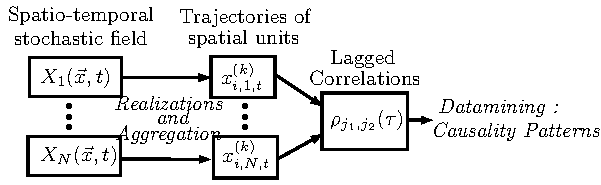
\includegraphics[width=\textwidth]{Figures/Theory/causality_regimes}
\medskip
\framecaption{}{\textbf{Structure de la méthodologie.} On part d'un champ stochastique dans le temps et l'espace. Un certain nombre de ses réalisations sont capturées, et mesurées sur des unités spatiales. \label{frame:causalityregimes:regimes}}
\end{mdframed}
\end{figure}
%%%%%%%%%%%%%


Avant de nous plonger dans l'exploration empirique de la méthode, donnons-en une vision intuitive pour mieux comprendre son lien avec la co-évolution. L'encadré~\ref{frame:causalityregimes:twovars} synthétise de manière stylisée des situation idéales pouvant se produire dans le cas de deux variables. De manière caricaturale, avec deux variables $X,Y$, le profil de $\rho_{\tau}\left[X,Y\right]$ est traduit selon les caractéristiques suivantes : existence d'un extremum ou non pour $\tau < 0$ et existence d'un extremum ou non pour $\tau > 0$. Les quatre possibilités sont illustrées et on représente les interactions entre variable sous forme graphique, dans le temps et de manière synthétique. 



%%%%%%%%%%%%%
\begin{figure}[h!]
\begin{mdframed}
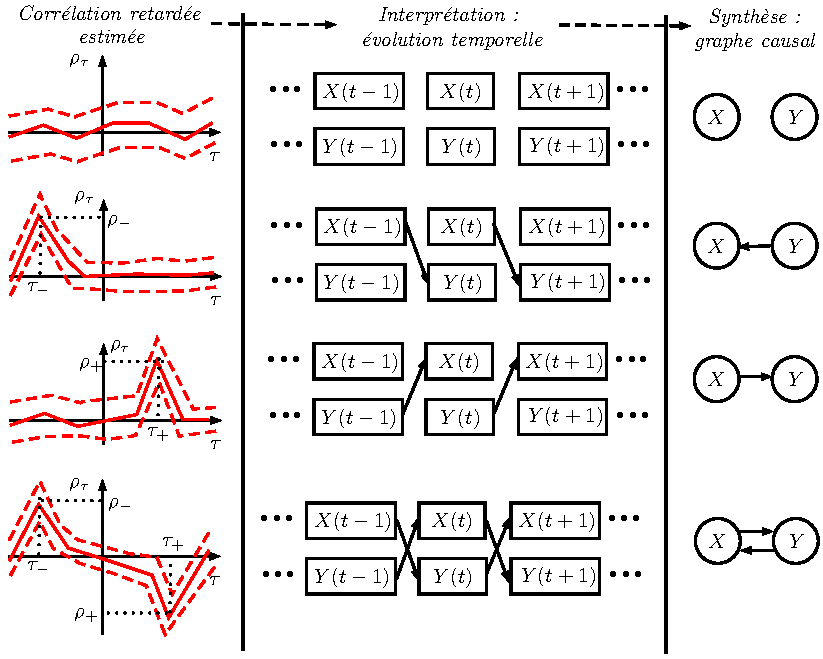
\includegraphics[width=\textwidth]{Figures/Theory/causality_twovars}
\medskip
\framecaption{}{\textbf{Illustration des situations possibles dans le cas de deux variables.} Pour simplifier, nous ne différencions les situations que par l'existence ou non d'un extremum pour les valeurs positives et négatives du délai $\tau$ (et ne prenons pas en compte le signe de la corrélation correspondante). Les lignes pointillées illustrent un seuil de significativité, par exemple un intervalle de confiance sur la corrélation estimée. On a donc quatre situations : aucun extremum significatif, existence de $\tau_-$, existence de $\tau_+$ et existence de $\tau_-$ et de $\tau_+$. Dans le premier, il n'y a pas de lien diachronique entre les variables (mais possiblement des corrélations simultanées, spécifiées par les doubles flèches verticales). Dans les deux suivants, l'une ``cause'' l'autre variable (nous utiliserons parfois ce raccourci sémantique pour commenter les résultats des analyses). Enfin dans la dernière, on a causalités circulaires : de tels motifs s'apparenteront à ce que l'on désignait conceptuellement par co-évolution.\label{frame:causalityregimes:twovars}}
\end{mdframed}
\end{figure}
%%%%%%%%%%%%%



\subsubsection{Emergence and a proxy to measure co-evolution ?}{Emergence et proxy pour la co-évolution ?}


% idee sur les repets : lors de l'agreg perd de l'information ? lie au maup..

Prenons également un court instant pour clarifier le statut épistémologique et ontologique attendu par l'application de cette méthode, et dans quelle mesure on peut espérer l'utiliser comme mesure indirecte de la co-évolution. La causalité de Granger est estimée à la fois \emph{dans le temps}, \emph{dans l'espace} et \emph{entre les répétitions}. Dans le cas où l'on observe un phénomène historique, on a une unique trajectoire et l'estimation est faite dans le temps et l'espace uniquement, mais dans tous les cas on passe de caractéristiques à l'échelle microscopique à une mesure macroscopique\footnote{Nous utilisons ici ces termes pour simplifier, il s'agit en fait d'un échelle donnée à une échelle supérieure qui dépend de l'étendue temporelle et spatiale totale}. Ainsi, on peut avoir des interactions microscopiques circulaires, mais émergence d'un sens de la causalité au niveau macroscopique, ou l'inverse. Rejoignant la question des populations et individus pour la définition de la co-évolution en biologie (voir~\ref{sec:epistemology}), pour laquelle les adaptations mutuelles émergent au niveau des espèces, nous postulons que la caractérisation des motifs de causalité est une manière de caractériser des dynamiques co-évolutives pour les systèmes territoriaux.


Est-il alors possible de répondre de manière équivoque à la question ``\textit{s'il y a co-évolution dans un cas particulier}''\footnote{A laquelle nous ajoutons : pour ces composantes, sur cette portée spatiale et temporelle et sur ces échelles spatiale et temporelle.} ? Cela se saurait si nous pouvions réinventer l'eau chaude mais qui se chauffe elle-même. Nous voulons dire par là, et nous le verrons dans les multiples développements, que de nombreux problèmes fondamentaux intrinsèques à l'étude des systèmes géographiques (la question des échelles, de la définition du système, des variables prises en compte, le problème de l'observation de trajectoire uniques, de données bruitées et éparses, le problème du MAUP, etc.) seront bien toujours présents, et que la question ci-dessus qui y est naturellement soustraite s'avère naïve. Mais nous verrons qu'il sera bien possible d'isoler des signaux clairs, et mettrons en évidence des cas où il existe un sens causal et d'autres où il y a circularité au niveau macroscopique.

% -> en conclusion partie II, revenir la dessus et preciser/clarifier la co-evol conceptuelle et la co-evol ``empirique'', enfin son proxy.



%%%%%%%%%%%%%%%
\subsection{Synthetic data}{Données Synthétiques}

\subsubsection{Auto-regressive time series}{Séries temporelles auto-régressives}

Illustrons les motifs qui peuvent être attendus, notamment ceux stylisés donnés précédemment en Encadré~\ref{frame:causalityregimes:twovars}, sur des données synthétiques avec une structure simple. L'idée est de générer des séries temporelles sur lesquelles le retard et le niveau de corrélation sont contrôlés, les résultats théoriques connus.


Soit $\mathbf{X}(t)$ un processus stochastique suivant l'équation d'auto-régression $\mathbf{X}(t) = \sum_{\tau > 0} \mathbf{A}(\tau) \cdot \mathbf{X}(t - \tau ) + \mathbf{\epsilon}(t)$. Dans le cas où $\mathbf{A}(\tau) = 0$ pour $\tau \neq \tau_0$ et $\mathbf{A}(\tau_0) = \left( {\begin{array}{cc} 0 & a_1 \\ a_2 & 0 \\ \end{array}} \right)$, le calcul des corrélations théoriques est immédiat (voir Appendice~\ref{app:sec:causalityregimes}), et on obtient, en notant $\mathbf{X} = (X,Y)$,
\[
\rho\left[X(\tau),Y(t-\tau)\right] = \left(1 + \frac{1}{a^2}\cdot \frac{\sigma^2}{\Varb{Y(t-\tau)}}\right)^{-\frac{1}{2}}
\]

et la corrélation simultanée tend vers zéro dans le temps :

\[
\rho\left[X(t),Y(t)\right] = a^{2t} \cdot \rho_0
\]


% comparaison correlation theorique / correlation empirique


%%%%%%%%%%%%%
\begin{figure}
	%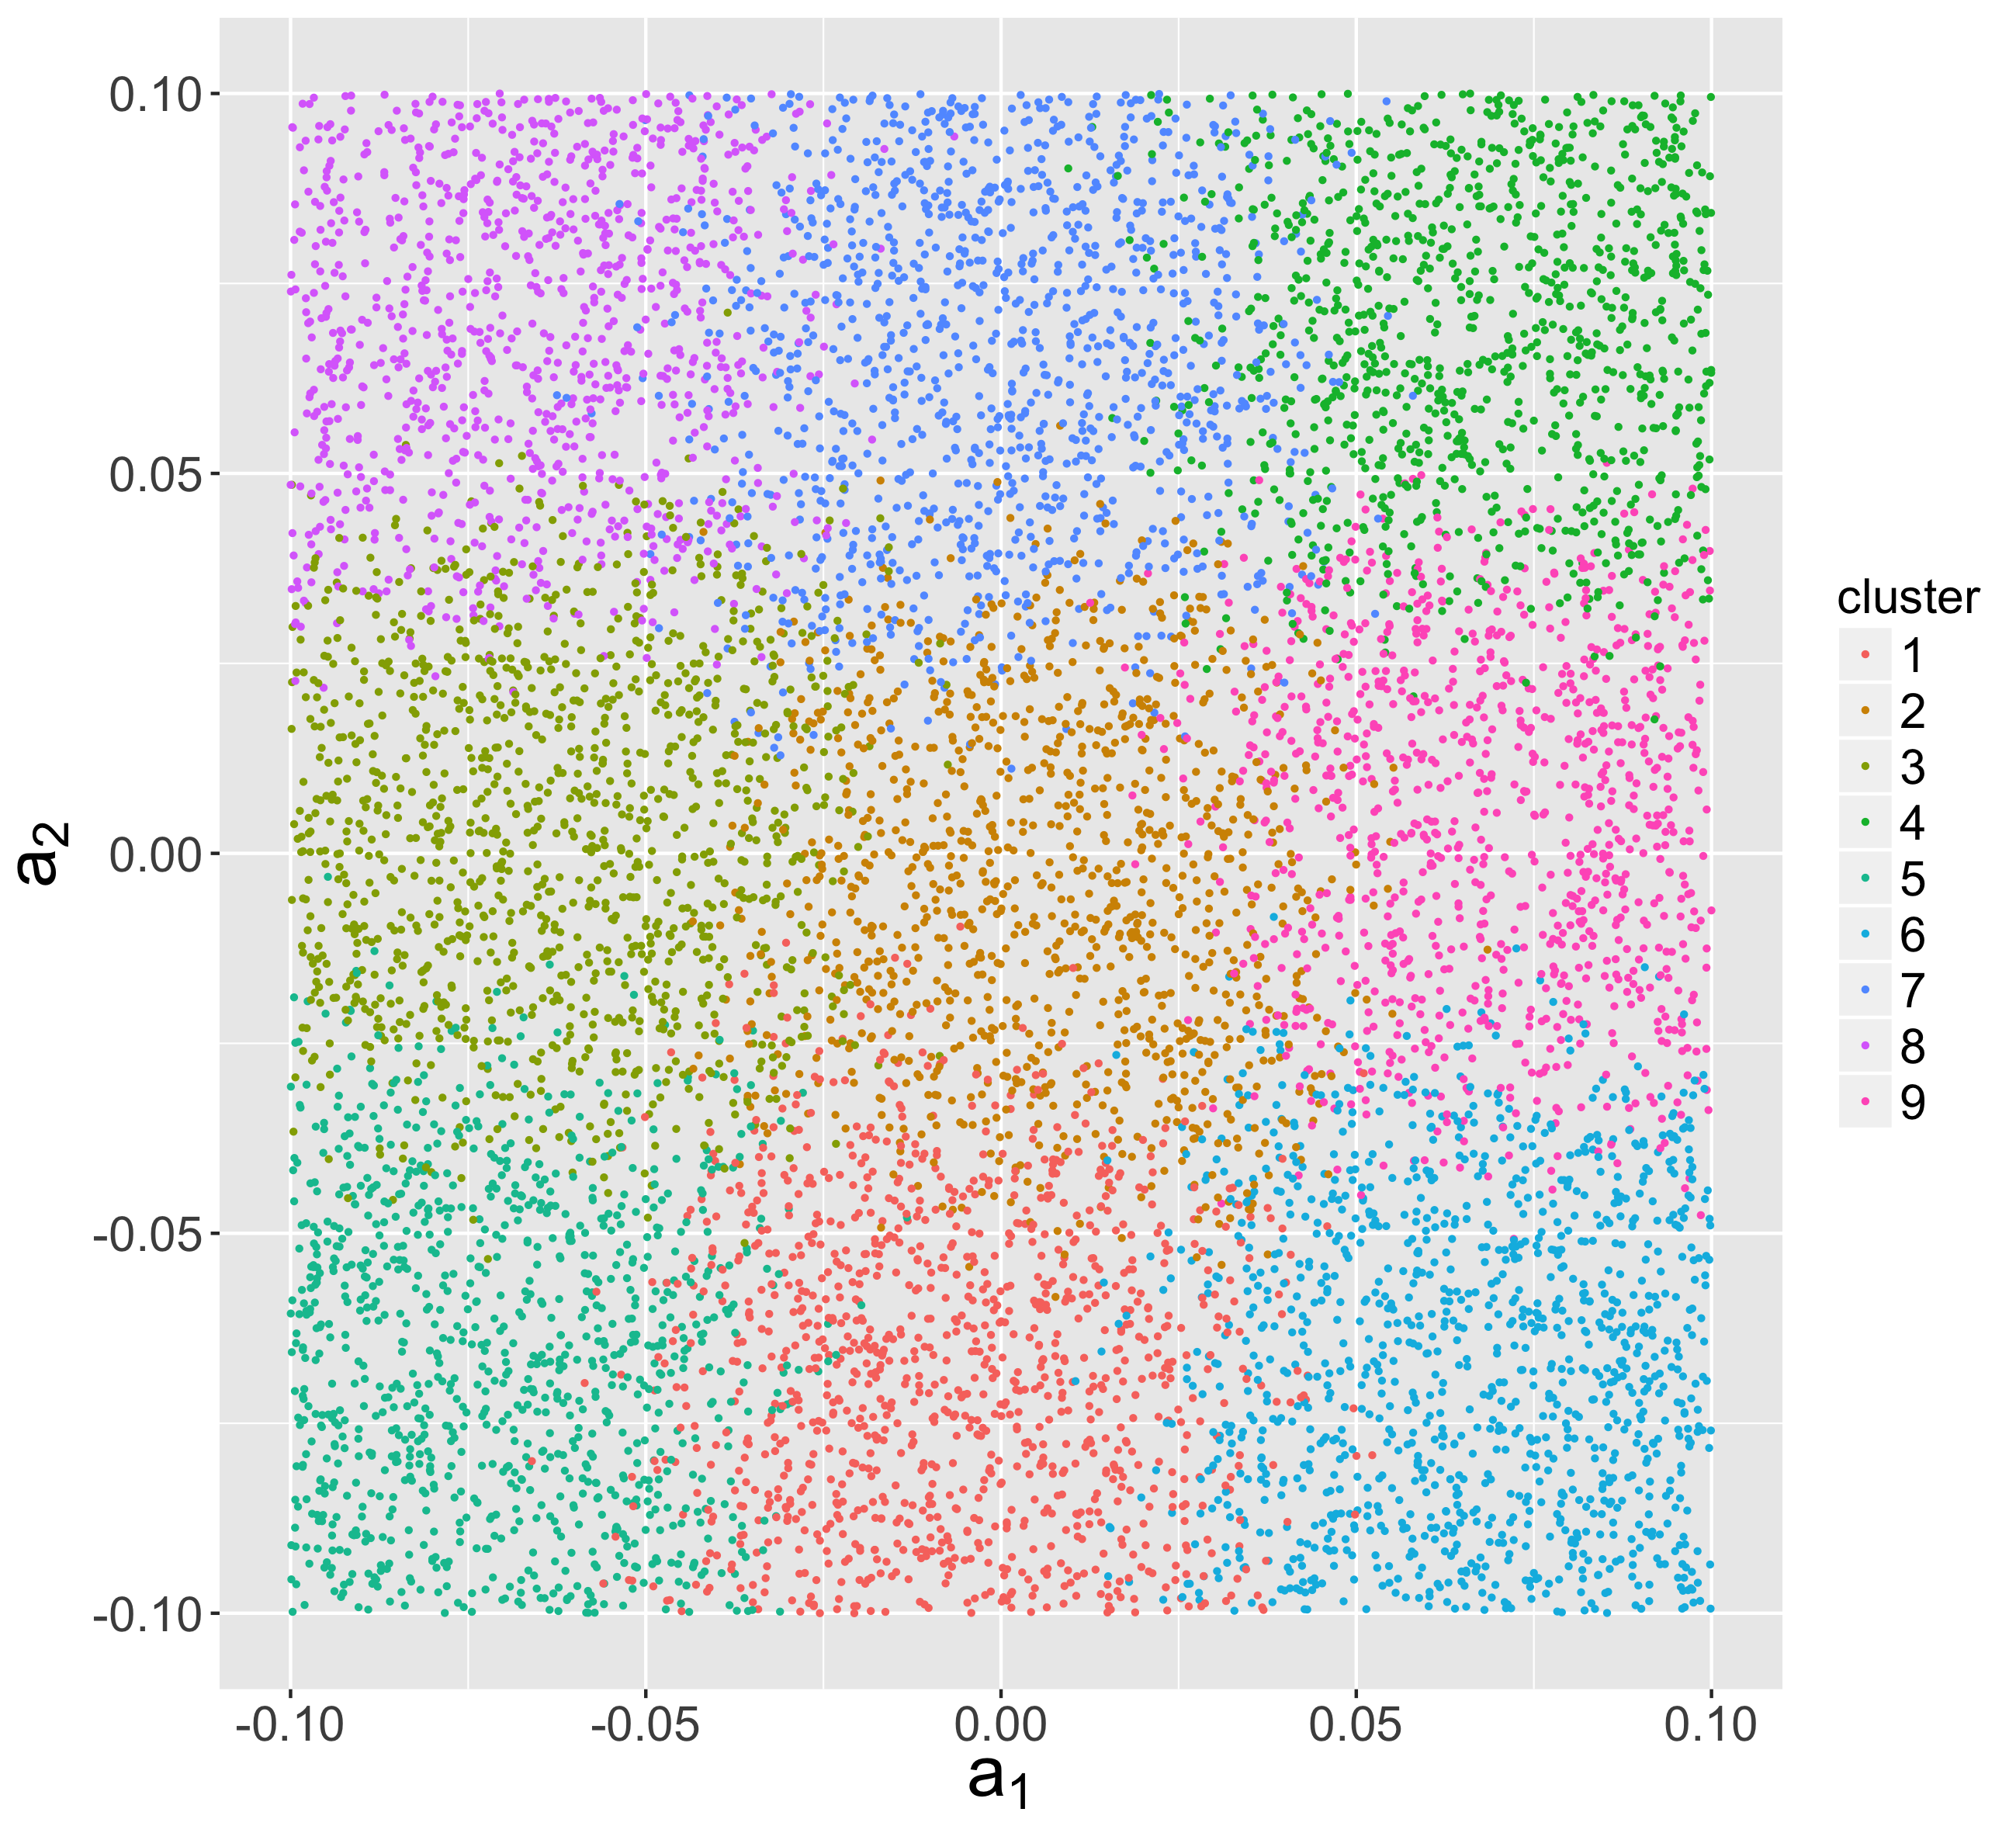
\includegraphics[width=0.48\linewidth]{Figures/CausalityRegimes/coefsclust_nbootstrap10000_maxai0_1_lag2nclust9.png}
	%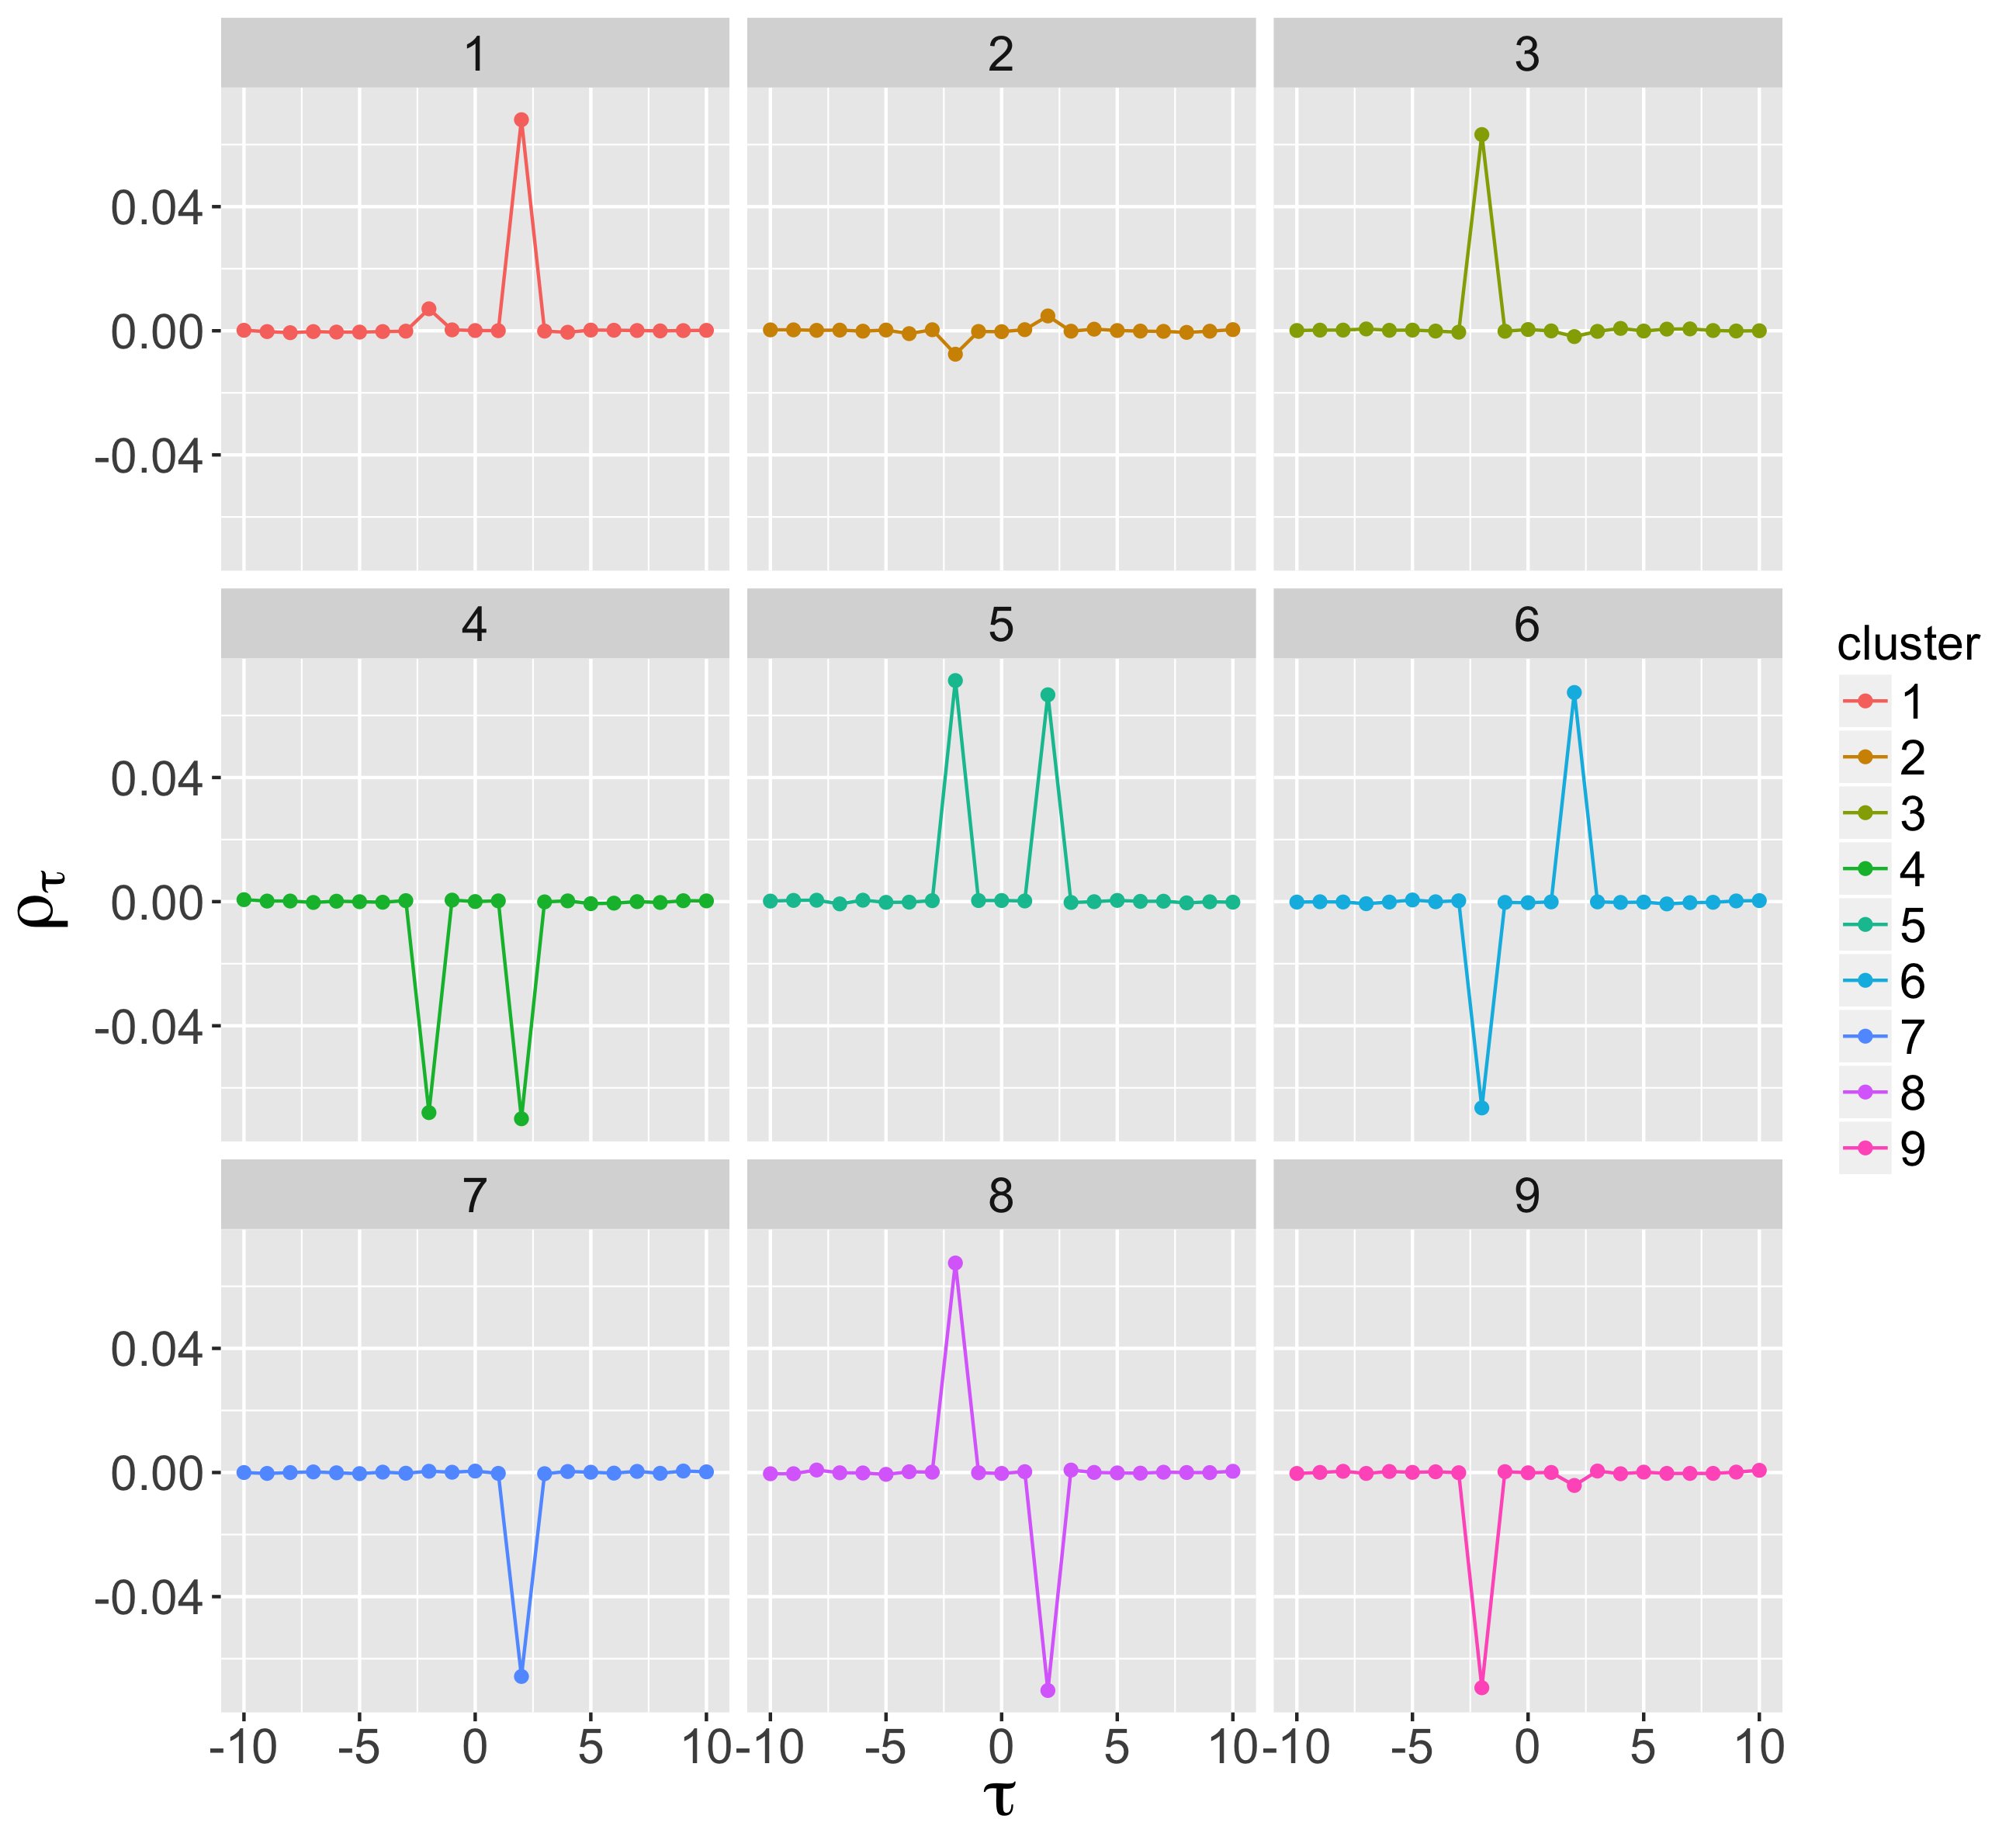
\includegraphics[width=0.48\linewidth]{Figures/CausalityRegimes/centertrajs_nbootstrap10000_maxai0_1_lag2nclust9.png}
	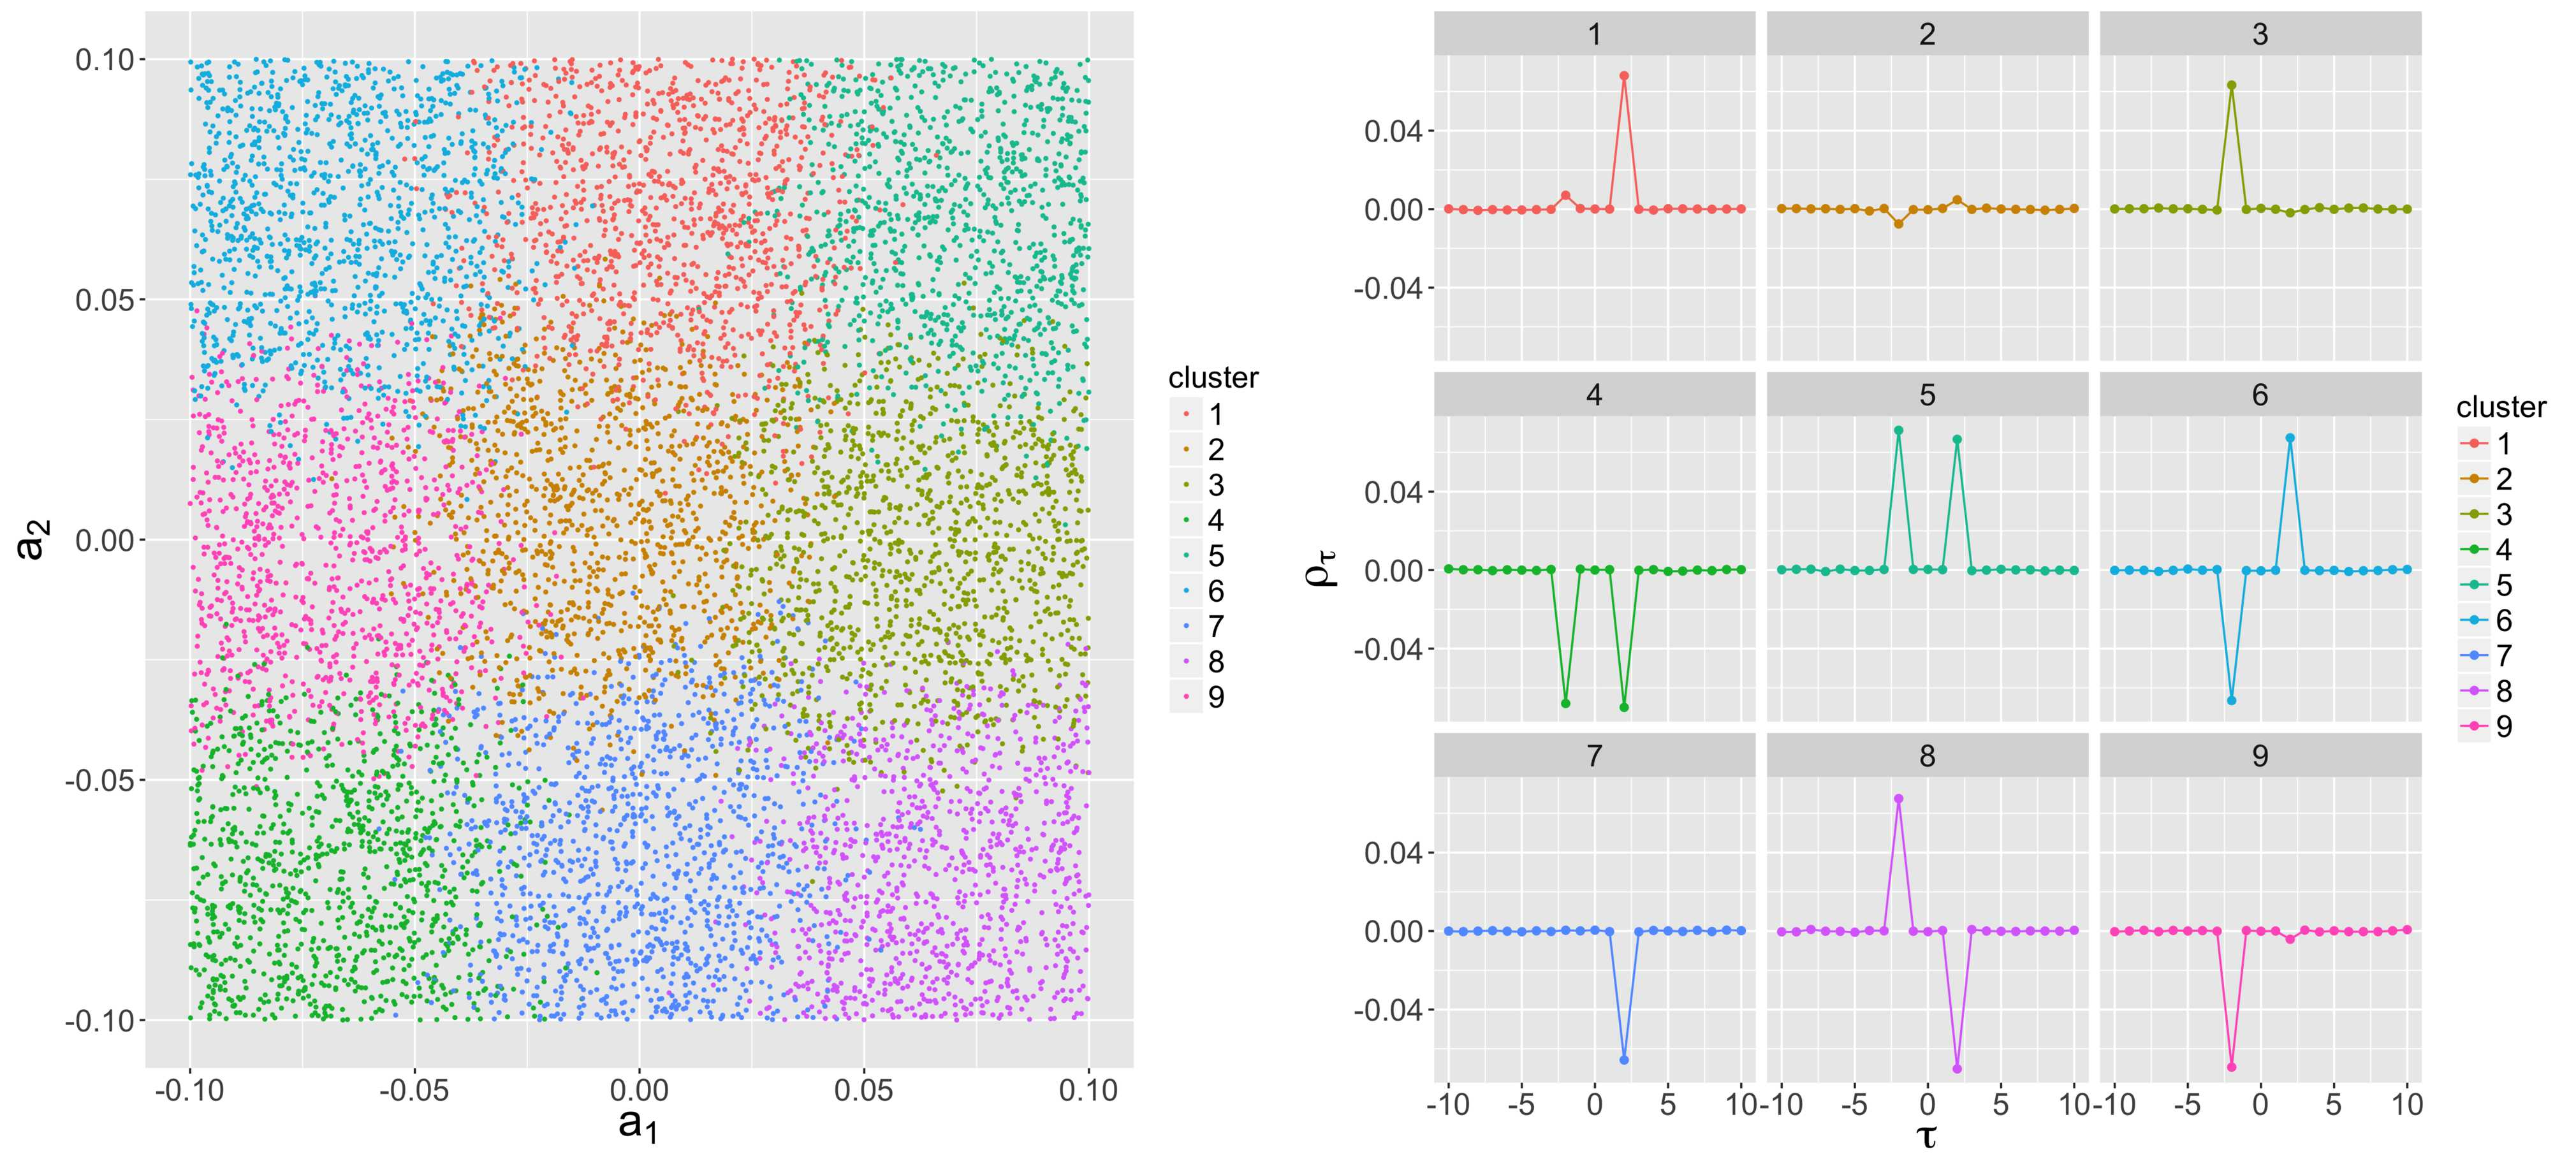
\includegraphics[width=\linewidth]{Figures/Final/4-2-2-fig-causalityregimes-arma.jpg}
	\caption[Auto-regressive time-series][Séries temporelles auto-régressives]{}{\textbf{Estimation des régimes de corrélation dans le cas de séries temporelles auto-régressives linéaires.} Résultats de la méthode de classification des régimes pour des processus AR simples. Nous simulons $b = 10000$ séries temporelles de longueur $t_f = 10000$, avec des coefficients aléatoires $(a_1,a_2) \in [-0.1,0.1]$ et un délai $\tau_0 = 2$. (\textit{Gauche}) Valeur des coefficients $(a_1,a_2)$, la couleur donnant le cluster obtenu ; (\textit{(Droite)}) Trajectoires de centroïdes correspondants.\label{fig:causalityregimes:arma}}
\end{figure}
%%%%%%%%%%%%%



\subsubsection{Urban growth model}{Modèle de croissance urbaine}

\bpar{
This method must first be tested and partially validated, what we propose to do on synthetic data, what allows a more refined knowledge of the behavior of models~\cite{raimbaulthalshs01514415}. Echoing the example of relations between transportation networks and territories that introduced the research question before, we generate stylized urban configurations in which network and density mutually interact, and for which causalities are not obvious \emph{a priori} knowing the parameters of the generative model. \cite{raimbault2014hybrid} describes and explores a simple model of urban morphogenesis (the RBD model) that fits perfectly these constraints. Indeed, explicative variables of urban growth, processes of network extension and the coupling between urban density and the network are relatively simple. However, except for extreme cases (for example when distance to the center solely determines land value, the network will depend on density in a causal way; when only the distance to the network counts, the causality will be inverted), mixed regimes do not exhibit obvious causalities. It is for this reason an ideal case to test if the method is able to detect some.
}{
Cette méthode doit dans un premier temps être testée et partiellement validée, ce que nous proposons de faire sur des données synthétiques, méthode qui permet une connaissance plus fine des comportements des modèles~\cite{raimbault2016generation}. En écho à l'exemple des relations entre réseaux de transport et territoires qui a permis d'introduire notre problématique précédemment, nous proposons de générer des configurations urbaines stylisées dans lesquelles réseau et densité s'influencent mutuellement, et pour lesquelles les causalités ne sont pas évidents \emph{a priori} étant donné les paramètres du modèle génératif. \cite{raimbault2014hybrid} décrit et explore un modèle simple de morphogenèse urbaine\footnote{Nous n'explorons pas ici le concept de morphogenèse, qui fera l'objet du Chapitre~\ref{ch:morphogenesis}, mais utilisons ce modèle comme producteur de données synthétiques.} (modèle RBD) répondant parfaitement à ces contraintes. En effet, les variables explicatives de la croissance urbaine, les processus d'extension du réseau et le couplage entre densité urbaine et réseau ne sont pas trop complexes. Cependant, hormis dans des cas extrêmes (par exemple lorsque la distance au centre détermine la valeur foncière uniquement, le réseau dépendra de manière causale de la densité, ou lorsque la distance au réseau seule compte, la causalité sera inversée), les régimes mixtes ne présentent pas de causalités évidentes : c'est donc un parfait cas pour tester si la méthode est capable d'en détecter  \comment[CC]{Alors la. c'est pas evident de vouloir demontrer quoi que ce soit a partir d'un modele que tu n'expliques pas. Si on ne comprend pas le fonctionnement, on n'est pas convaincu par ton histoire de regimes mixtes. Au contraire, on se dit que ce qui est difficile a demeler, c'est les donnees empiriques et que les donnees synthetiques tu devrais pouvoir les controler beaucoup plus pour tester la methode...}. Les données synthétiques nous permettent de contrôler la cohérence dans les cas où la relation est attendue.
}


%%%%%%%%%%%%%
\begin{figure}[h!]
\begin{mdframed}
Le modèle RBD suppose une grille de côté $N$, dont les cellules ont un état binaire (occupée ou non). Dans la version utilisée, il existe un unique centre urbain (noeud particulier du réseau) et le réseau de transport est initialement nul. Chaque cellule (patch) est caractérisée par les variables $x_d$ (densité dans un rayon fixé), $x_r$ (distance à la route la plus proche) et $x_c$ (distance au centre via le réseau, qui permettent de calculer une valeur $U = \sum w_k x_k$.

A chaque pas de temps :
\begin{itemize}
	\item Les $N_G$ cellules avec plus grande valeur sont occupées de manière simultanée
	\item Si une cellule nouvellement peuplée est à une distance au réseau supérieure à un seuil $d_r$, celle-ci est connectée au réseau par une nouvelle route prenant le chemin le plus court
\end{itemize}

% here example de configs
%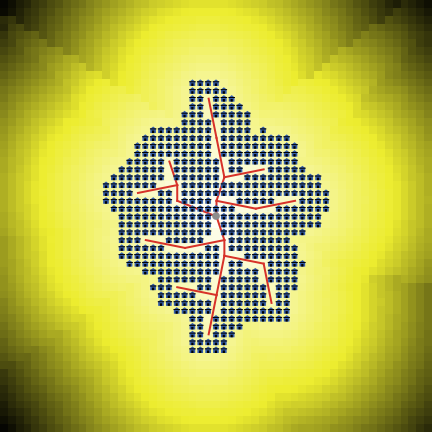
\includegraphics[width=0.32\linewidth]{Figures/CausalityRegimes/ex_60_wdens0_wroad1_wcenter1_seed272727}
%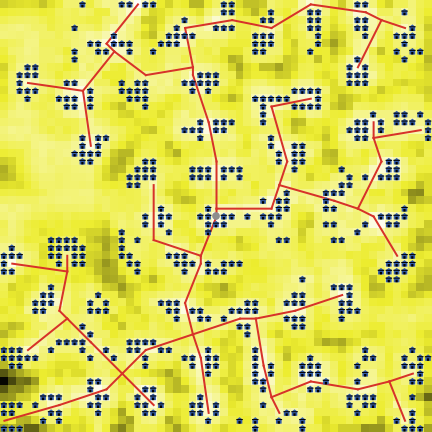
\includegraphics[width=0.32\linewidth]{Figures/CausalityRegimes/ex_60_wdens1_wroad1_wcenter0_seed272727}
%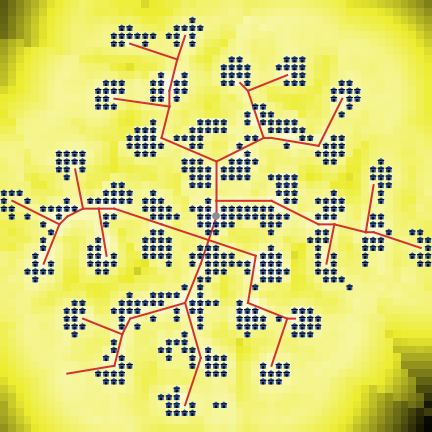
\includegraphics[width=0.32\linewidth]{Figures/CausalityRegimes/ex_60_wdens1_wroad1_wcenter1_seed272727}
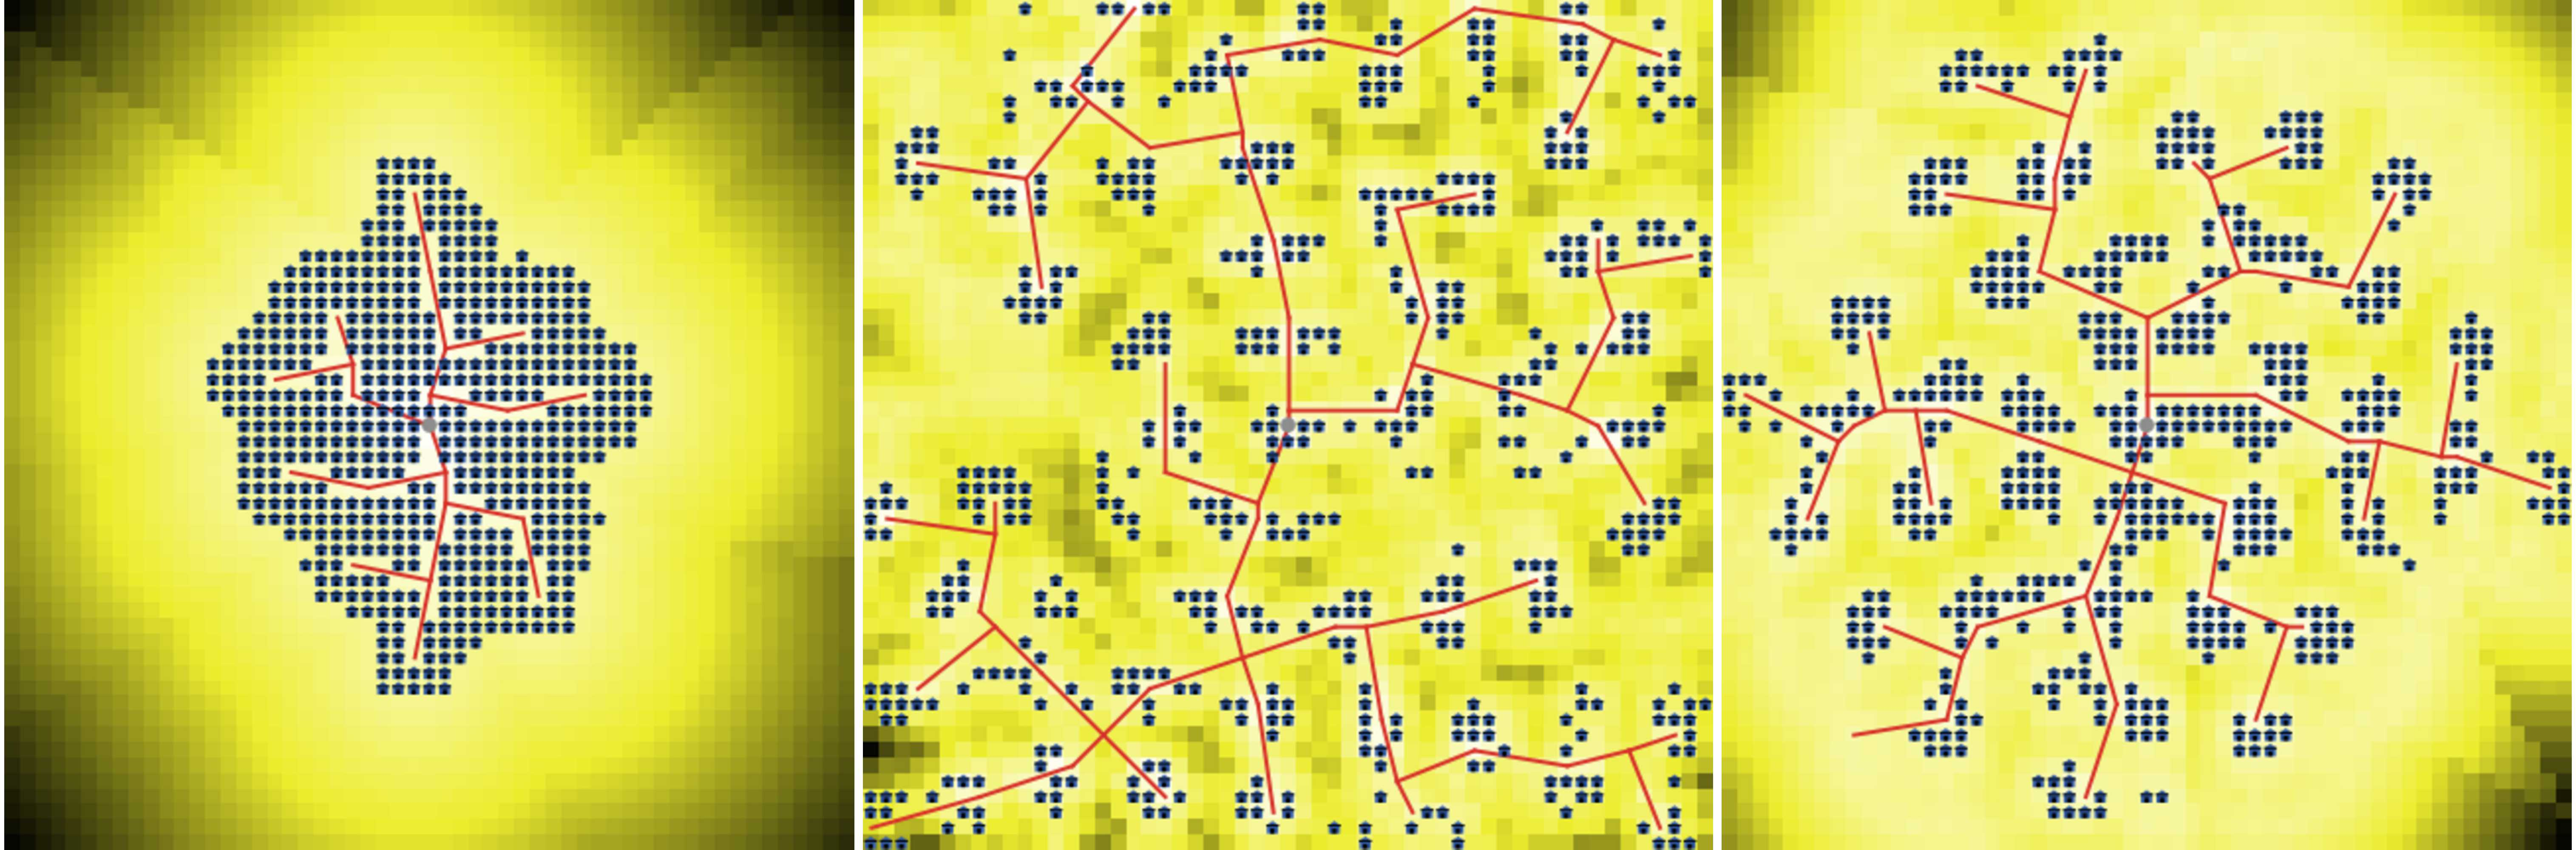
\includegraphics[width=\linewidth]{Figures/Final/4-2-2-frame-causalityregimes-rdb.jpg}
 Exemples de configurations finales variées, obtenues avec les paramètres de poids $(w_{d},w_{c},w_{r})$ valant respectivement $(0,1,1)$,$(1,0,1)$, et $(1,1,1)$.

\medskip

\framecaption{}{\textbf{Description du modèle RBD.}\label{frame:causalityregimes:rbd}}
\end{mdframed}
\end{figure}
%%%%%%%%%%%%%





\bpar{
 We use an applied implementation\footnote{available on the open repository of the project at \\\texttt{https://github.com/JusteRaimbault/CityNetwork/tree/master/Models/Simple/ModelCA}} of the original model, allowing to capture the values of studied variables for each cell of the cellular automaton and for each time step, and to calculate the lagged correlations in the sense described before, between variables of the model. We explore a grid of the parameter space of the RBD model, making the weight parameters for density, distance to center and distance toi network vary\footnote{The model works the following way: a value of cells is determined by the weighted average of these different explicative variables, value that determines the growth of new patches at the next time step.}, that we write respectively $(w_{d},w_{c},w_{r})$, in $\left[0;1\right]$ with a step of $0.1$. Other parameters are fixed to their default values given by~\cite{raimbault2014hybrid}. For each parameter value, we proceed to $N=100$ repetitions, what is enough for a good convergence of indicators. Explorations are done with the OpenMole software~\cite{reuillon2013openmole}, the large number of simulations (1,330,000) implying the use of a computation grid. We compute for all patches the lagged correlations with the unbiased Pearson estimator between the variations of the following variables\footnote{Computing the correlations directly on the variables makes no sense since their value has no absolute meaning.}: local density, distance to center and distance to network. The figure~\ref{fig:exrdb}  shows the behavior of $\rho_{\tau}$ for each couple of variable (undirected, $\tau$ taking negative and positive values), for the combination of extreme values of parameters. We can already see different regimes emerge: for example, $(1,0,1)$ leads to a causality of density on distance to center with a lag $\tau=1$, and a negative causality of density on distance to network with the same lag, whereas distance to the center and to the network are correlated in a synchronous manner.
}{
Nous utilisons une implémentation adaptée\footnote{disponible sur le dépôt ouvert du projet à\\\texttt{https://github.com/JusteRaimbault/CityNetwork/tree/master/Models/Simple/ModelCA}} du modèle initial, permettant de capturer les valeurs des variables étudiées pour chaque patch et à chaque pas de temps et de calculer les correlations retardées entre variables au sein du modèle. Nous explorons une grille de l'espace des paramètres du modèle RBD, faisant varier les paramètres de poids de la densité, de la distance au centre et de la distance au réseau \comment[CC]{ca marche pas de nous parler de parametre dont on ne connait pas le role dans le modele. C'est dommage} \footnote{Le modèle fonctionne de la façon suivante : une valeur des patches est déterminée par la moyenne pondérée de ces différentes variables explicatives, valeur qui détermine la croissance de nouveaux patches à l'instant suivant.}, que l'on note respectivement $(w_{d},w_{c},w_{r})$, dans $\left[0;1\right]$ avec un pas de 0.1. Les autres paramètres sont fixés à leur valeurs par défaut données par \cite{raimbault2014hybrid}. Pour chaque valeur des paramètres, nous procédons à $N=100$ répétitions ce qui est suffisant pour une bonne convergence des indicateurs. Les explorations sont effectuées via le logiciel OpenMole~\cite{reuillon2013openmole},\comment[FL]{ce n'est pas suffisant ni rendre justice a ce logiciel (il y a un gros travail computationnel dans ta these, a bien mettre en valeur)} le grand nombre de simulations (1,330,000) nécessitant l'utilisation d'une grille de calcul. Nous calculons sur l'ensemble des patches\comment[FL]{qu'est ce qu'un patch ?} les corrélations retardées par estimateur de Pearson non biaisé entre les variations des variables suivantes\footnote{Calculer les corrélations sur les variables directement n'a pas de sens puisque leur valeur n'en a pas en absolu.} : densité locale, distance au centre et distance au réseau  \comment[CC]{Je croyais que ces trois variables etaient les parametres que tu faisais varier.  $(w_{d},w_{c},w_{r})$. Tres confus du coup...}. La Fig.~\ref{fig:causalityregimes:exrdb} montre le comportement de $\rho_{\tau}$ pour chaque couple de variable \comment[CC]{s} (non dirigé, $\tau$ prenant des valeurs négatives et positives), pour les combinaisons des valeurs extrêmes des paramètres. On peut voir déjà différents régimes émerger : par exemple, $(1,0,1)$ conduit à une causalité de la densité sur la distance au centre avec un retard 1, et une causalité négative de la densité sur la distance au réseau avec le même retard, tandis que distance au centre et au réseau sont corrélés de manière synchrone. \comment[FL]{c'est trop rapide, encore}
\comment[CC]{d'accord avec Florent. La lecture de la figure seule ne suffit pas a faire emerger la comprehenson du lecteur, surtout etant donne que la figure est dense, peu intuitive et assez peu lisible. On veut savoir quels sont les resultats majeurs, a quoi ils correspondent sur la figure (tu peux faire des encadres ou un truc comme ca) et ce que ca signifie pour la qualite de ta mesure de correlation retardee}
}





%%%%%%%%%%%%%%%
\begin{figure}
\vspace{-0.5cm}
%\includegraphics[width=\linewidth]{Figures/CausalityRegimes/synth_extreme.jpg}
\includegraphics[width=\linewidth,height=0.9\textheight]{Figures/Final/4-2-2-fig-causalityregimes-exrdb.jpg}
\vspace{-0.8cm}
\caption[Correlation in the RBD model][Correlations dans le modèle RDB]{\textbf{Correlations in the RBD model.} \textbf{(First row)} Example of different final configurations, obtained with $(w_{d},w_{c},w_{r})$ being respectively $(0,1,1)$,$(1,0,1)$, and $(1,1,1)$. \textbf{(Second row)} Lagged correlations, for each combination of parameters in $\{0,1\}$, as a function of the lag $\tau$. The different colors correspond to each couple of variables: distance to the center (\texttt{ctr}, $C$), density (\texttt{dens}, $D$) and distance to the network (\texttt{rd}, $R$). The dots show the extent on all the repetitions of the model (estimators on $i$ and $t$ only).\label{fig:causalityregimes:exrdb}}{\textbf{Correlations retardées dans le modèle RDB.} Corrélations retardées, pour chaque combinaison des valeurs extrêmes pour l'ensemble des paramètres $w_r,w_c,w_d$. Chaque graphe donne la corrélation $\rho_{\tau}$ en fonction du retard $\tau$. Les différentes couleurs correspondent à chaque couple de variables : distance au centre (\texttt{ctr}), densité (\texttt{dens}) et distance au réseau (\texttt{rd}). Les points correspondent aux corrélations individuelles pour chaque répétition du modèle (estimateurs sur $i$ et $t$), tandis que les courbes donnent l'estimateur complet sur l'ensemble des répétitions également. Pour chaque graphe, nous donnons en correspondance directe une configuration finale, et l'interprétation de terme de motifs de causalité sous forme d'un graphe entre les variables. La couleur des liens dirigés donne le signe de la relation (rouge pour corrélation négative, verte pour corrélation positive).\label{fig:causalityregimes:exrdb}}
\end{figure}
%%%%%%%%%%%%%%%

% \comment[CC]{par contre tu peux mettre 2 par 2 une image du reseau-territoire en regard avec le graph des correlations.}






\paragraph{Causality regimes}{Régimes de causalité}

\bpar{
To study these behaviors in a systematic way, we propose to identify regimes endogenously, by using non-supervised classification. We apply a \emph{k-means} clustering, robust to stochasticity (5000 repetitions), with the following features: for each couple of variables, $\textrm{argmax}_{\tau} \rho_{\tau}$ and $\textrm{argmin}_{\tau} \rho_{\tau}$ if the corresponding value is such that $\frac{\rho_{\tau}-\bar{\rho}_{\tau}}{\left|\bar{\rho}_{\tau}\right|} > \theta$ with $\theta$ threshold parameter, 0 otherwise. The inclusion of supplementary features of values of $\rho_{\tau}$ does not significantly changes the results, these are therefore not taken into account to reduce the dimension. The choice of the number of clusters $k$ is generally a difficult problem in this kind of approach~\cite{hamerly2003learning}. In our case the system exhibit an convenient structure: the curves of inter-cluster variance proportion and its derivative in figure~\ref{fig:clustering}, as a function of $k$ for different values of $\theta$, show a transition for $\theta = 2$, what gives for the corresponding curve a break around $k=6$. A visual screening of clusters in a principal plan confirms the good quality of the classification for these values. A class corresponds then to a \emph{causality regime}, for which we can represent the phase diagram as a function of model parameters, and also cluster centers profiles (computed as the barycenter in the full initial space) in figure~\ref{fig:clustering}.
}{
Nous démontrons à présent qu'il est possible d'établir une typologie endogène des comportements des corrélations retardées. Afin d'étudier ces comportements de manière systématique, nous proposons d'identifier des régimes de manière endogène, en procédant à un apprentissage non-supervisé. Nous appliquons une classification des \emph{k-means},\comment[FL]{oourquoi cette methode ?} robuste à la stochasticité (5000 répétitions)\comment[FL]{ce seuil ?}, avec les points caractéristiques (\emph{features}) suivants : pour chaque couple de variable, $\textrm{argmax}_{\tau} \rho_{\tau}$ et $\textrm{argmin}_{\tau} \rho_{\tau}$ si la valeur correspondante est telle que $\frac{\rho_{\tau}-\bar{\rho}_{\tau}}{\left|\bar{\rho}_{\tau}\right|} > \theta$ avec $\theta$ paramètre de seuil, 0 sinon. L'inclusion des \emph{features} (variables caractéristiques) supplémentaires des valeurs de $\rho_{\tau}$ n'influence pas significativement les résultats, celles-ci n'ont pas été prises en compte pour réduire la dimension. Le choix du nombre de clusters $k$\comment[FL]{il y a deja en cette question avant sens que tu souleves ce probleme : harmoniser} est en général épineux dans ce genre de problème~\cite{hamerly2003learning}, dans notre cas le système possède une structure agréable\comment[FL]{sens ?} : les courbes de la proportion de variance inter-cluster et de sa dérivée en Fig.~\ref{fig:causalityregimes:clustering}, en fonction de $k$ pour différentes valeurs de $\theta$, présentent une transition pour $\theta = 2$, ce qui donne pour cette courbe une rupture à $k=5$. Un examen visuel des clusters dans un plan principal confirme la bonne qualité de la classification pour ces valeurs. Une classe correspond alors à un \emph{régime de causalité}, dont nous pouvons représenter le diagramme de phase en fonction des paramètres du modèle, ainsi que les trajectoires des centres des clusters (calculées comme barycentre dans l'espace complet initial) en Fig.~\ref{fig:causalityregimes:clustering}.
}



\paragraph{Interpretation}{Interprétation}

\bpar{
 The behavior obtained is interesting, as regions in the diagram corresponding to the different regimes are clearly delimited and connected. For example, we observe the emergence of regime 6 in which distance to network causes strongly the density in a negative way, but distance to the center causes distance to the network. Its maximal extent on $(w_d,w_r)$ is for an intermediate value $w_r=0.7$. Thus, to maximize the impact of network on density, the corresponding weight must not be maximized, what can be counter-intuitive at first sight. It illustrates the utility of the method in the case of circular causal relations difficult to entangle a priori. The regime 5, in which distance to network influences the density the same way, but the relation between distance to center and to the network is inverted, is also interesting, and predominates for low $w_r$ values. The regime 1 is an extreme one and corresponds to an isolated situation in which distance to the center has no role: this aspect dominates then totally the other interaction processes between density and network. This application on synthetic data demonstrate on one hand the robustness of the method given the consistence of obtained regimes, and realizes this way a much more finer qualification of model behavior than the one done in the original paper. In this precise case, it can be taken as an instrument of knowledge for relations between networks and territories in itself, allowing the test of assumption or the comparison of processes in the stylized model.

}{
Nous proposons finalement d'interpréter les régimes obtenus. Le comportement obtenu est particulièrement intéressant : les régions du diagramme correspondant aux régimes sont clairement délimitées et connexes. Par exemple, on observe l'émergence du régime 6\comment[FL]{?} où la distance au réseau cause fortement la densité de manière négative, mais la distance au centre cause la distance au réseau, régime dont l'étendue maximale sur $(w_d,w_r)$ est pour une valeur intermédiaire $w_r=0.7$ \comment[CC]{pas clair... du tout! 'cause' a mon sens ne veut pas dire grand chose, on a besoin du mecanisme pour comprendre le lien. Et deuxiemement toute l'interpretation est perdue si l'on a pas compris le fonctionnement du modele, on est oblige de te croire sur parole $\neq$ de la science}. Ainsi, pour maximiser l'impact du réseau sur la densité, il ne faut pas maximiser le poids correspondant, ce qui peut paraître contre-intuitif en premier abord : cela illustre l'intérêt de la méthode dans le cas de relations circulaires difficiles à démêler a priori. Le régime 5, où la distance au réseau influence la densité de la même manière, mais la relation entre distance au centre et route est inversée, est tout aussi intéressant, et est prédominant dans les faibles $w_r$. Le régime 1, extrême, correspond à une situation isolée dans laquelle la distance au centre n'importe pas : cet aspect domine alors totalement les autres processus d'interaction entre densité et réseau. Cette application sur données synthétiques démontre ainsi d'une part la robustesse de la méthode vu la cohérence des régimes obtenus, et constitue aussi une qualification beaucoup plus précise des comportements du modèle que celle réalisée dans l'article initial. Dans ce cas précis, il peut s'agir d'un instrument de connaissance des relations entre réseaux et territoires en lui-même, permettant le test d'hypothèses ou la comparaison de processus dans le modèle stylisé.\comment[FL]{le lecteur (moi en tout cas) est perdu.}[(CC) ... moi aussi. sur tes interpretation des differents regimes, c'est bien de les detailler un par un, mais personnellement je n'ai pas vu ce qui dans les figures te permettait de le dire. ex: ``regime 1, la distance au centre ne joue pas.'' je regarde les graphiques du bas de la figure 20 et pourtant je vois des correlations non-nulles entre ctr et les autres variables, a tau = 0 mais pas seulement, donc 1/ je suis perdue sur ce cluster en particulier et 2/ je suis perdue pour les autres car je ne saurai pas non plus ou trouver les elements sur lesquels tu t'appuies.]
}



%%%%%%%%%%%%%%%
\begin{figure}
%\includegraphics[width=0.59\linewidth]{Figures/CausalityRegimes/clusters-paramfacet_valuesFALSEtheta2_k6}\\
%\includegraphics[width=\linewidth]{Figures/CausalityRegimes/clusters-centertrajs-facetclust_valuesFALSEtheta2_k6}]
\includegraphics[width=\linewidth]{Figures/Final/4-2-2-fig-causalityregimes-clustering.jpg}
\caption[Identification of interaction regimes][Identification de régimes d'interactions]{\textbf{Identification of regimes of interaction.} \textbf{(Top left)} Inter-cluster variance as a function of cluster number. \textbf{(Top middle)} Derivative of the inter-cluster variance. \textbf{(Top right)} Features in a principal plan (81\% of variance explained by the two first components)\textbf{(Bottom left)} Phase diagram of regimes in the space $(w_{d},w_{c},w_{r})$, $w_r$ varying between the different sub-diagrams of $(w_{d},w_{c}$. \textbf{(Bottom right)} Corresponding profiles of centroids.\label{fig:causalityregimes:clustering}}{\textbf{(Haut)} Diagramme de phase des régimes dans l'espace $(w_{d},w_{c},w_{r})$, $w_r$ variant entre les différents sous-diagrammes de $(w_{d},w_{c}$. \textbf{(Bas)} Trajectoires correspondantes des centroïdes.\label{fig:causalityregimes:clustering}}
\end{figure}
%%%%%%%%%%%%%%%

\comment[FL]{idem}[(CC) je dirais qu'ici le probleme c'est qu'on a une figure pas evidente projetee ici sans contexte. Je la mettrai plutot apres le texte qui l'introduit]












%--------------------------------------------------------









%%%%%%%%%%%%%%%%%%%%%%%
\subsection{Network-territory relations in South Africa}{Relations Réseaux-territoires en Afrique du Sud}



\bpar{
We assum that territorial dynamics and network dynamics responded differently to these. We expect to learn from these project informations on interactions at long time scale and large spatial scale, in a very particular context of constrained growth.
}{
Nous démontrons à présent les potentialités de notre méthode sur des données géo-historiques sur le temps long, pour le cas du réseau ferré en Afrique du Sud au cours du 20ème siècle. En faisant l'hypothèse que les territoires et les réseaux réagissent différemment aux événements historiques, les motifs de causalité devraient informer sur leur relations sur le temps long.
}


\subsubsection{Context}{Contexte}


\bpar{
Transportation Networks can be leveraged as a powerful socio-economic control tool, with even more significant outcomes when it percolates to their interaction with territories. The case of South Africa is an accurate illustration, as \cite{baffi:tel-01389347} shows that during apartheid railway network planning was used as a racial segregation tool by shaping strongly constrained mobility and accessibility patterns. In particular, it is shown qualitatively that dynamics between territories and networks profoundly changed at the end of the apartheid, transforming a tool of planed segregation (network shaped was optimized to minimize unwanted accessibility) into an integration tool thanks to recent changes in network topology patterns. We propose to investigate the potential \emph{structural} properties of this historical process, by focusing on dynamical patterns of interactions between the railway network and city growth. More precisely, we try to establish if the segregative planning policies did actually modify the trajectory of the coupled system, what would correspond to deeper and wider impacts. 
}{
Les réseaux de transport peuvent être utilisés comme un puissant outil de contrôle des populations, avec des effets encore plus significatifs lorsque ceux-ci perturbent les relations avec les territoires. Le cas de l'Afrique du Sud est une illustration pertinente, puisque \cite{baffi:tel-01389347} montre que lors de l'apartheid la planification du réseau ferré était utilisée comme un outil de ségrégation raciale par l'établissements de motifs de mobilité et d'accessibilité fortement contraints. En particulier, il est montré qualitativement que les dynamiques entre réseaux et territoires ont profondément changé à la fin de l'apartheid, transformant un outil de ségrégation planifiée (une forme de réseau optimisée pour minimiser une accessibilité non désirée) en un outil d'intégration grâce à des changement récents dans la topologie du réseau. Nous étudions ici les potentielles propriétés \emph{structurelles} de ce processus historique, en se concentrant sur les motifs dynamiques des interactions entre le réseau ferré et la croissance des villes. Plus précisément, nous essayons d'établir si les politiques de planification ségrégatives ont effectivement modifié la trajectoire du système couplé, ce qui correspondrait à des impacts plus larges et profonds que leurs effets immédiats.
}



\subsubsection{Data}{Données}


\bpar{
We use a comprehensive database covering the full South African railway network from 1880 to 2000 with opening and closing dates for each station and link, together with a city database spanning from 1911 to 1991 for which consistent ontologies for urban areas have been ensured. These database are described by~\cite{baffi:tel-01389347}, but they are not open so we make available only the aggregated data we used in the analysis.
}{
Nous utilisons une base de données complète couvrant l'ensemble du réseau ferré Sud-Africain de 1880 à 2000 avec les dates d'ouverture et de fermeture pour chaque station et liaison, couplée à une base de données pour les villes s'étendant de 1911 à 1991 pour laquelle des ontologies consistantes pour les aires urbaines ont été assurées. Ces bases de données sont décrites par~\cite{baffi:tel-01389347}, mais ne sont pas ouvertes. Pour respecter notre exigence d'ouverture, nous ne mettons ainsi à disposition que les données agrégées utilisées dans l'analyse.
}



\subsubsection{Network Measures}{Mesures de réseau}

\bpar{
First, a dynamical study of network measures seem to confirm the hypothesis: a trend rupture in closeness centrality (defined for a node as the average travel time to other nodes) at a roughly constant network size evolution, at a date corresponding to the beginning of official segregative policies, suggests that the planning process after this date had in the best case no global effect on network performance, and in the worst case had intended negative effects on accessibility with the aim to physically segregate more.
}{
Une analyse préliminaire consiste à regarder l'évolution dynamique des mesures de réseau, celles-ci pouvant témoigner de ruptures dans les propriétés structurelles du réseau et donc de mutations historiques profondes. L'évolution de certaines propriétés du réseau, comme les distributions de la centralité ou de l'accessibilité, peut témoigner de l'existence d'une planification les ayant influencées. Nous montrons en Figure~\ref{fig:causalityregimes:network} l'évolution des mesures de réseau dans le temps, correspondant aux mesures les plus basiques de celles définies en~\ref{sec:staticcorrelations}. \comment[CC]{peut-etre aussi rappeler la forme du reseau avec 2-3 cartes de Solene?}[(JR) par principe aucun graphe exterieur (sauf le xkcd ;) ) - vais essayer de resumer ca] La centralité de proximité, que nous définissons comme le temps moyen de trajet vers les autres noeuds, présente un comportement intéressant. En effet, la taille du réseau et les valeurs moyennes des centralités présentent un comportement concordant, qui correspond à l'expansion initiale du réseau. Par contre, la tendance de la hiérarchie de la centralité de proximité à se réduire est soudainement rompue à la date correspondant à l'officialisation des politiques ségrégatives en 1951, alors que taille et forme géométrique globale du réseau, traduite par l'efficience, restent constants. \comment[CC]{c'est la these de Solene plus que la tienne, mais il manque un maillon explicatif entre "politique segregative" et "impact sur le reseau ferre". Comment une politique de separation des groupes dans l'espace influence-t-elle tout le reseau national de voies de chemin de fer? Les bantoustan, la mobilite differenciee, les zones tampons etc. A rappeler pour les non specialistes de l'Afrique du Sud et de son histoire politique.} Ainsi, dans le meilleur des cas la planification après cette date est une coincidence avec la variation de cette propriété. Dans le pire des cas elle est en effet responsable de cette rupture de tendance, c'est à dire a eu les effets escomptés sur l'accessibilité, dans le but d'empêcher la diminution de la ségrégation, puisque plus la hiérarchie est faible plus le réseau est égalitaire.
}


%%%%%%%%%%%%%%
\begin{figure}[h!]
%\includegraphics[width=0.42\linewidth]{Figures/CausalityRegimes/nw_nwSize}
%\includegraphics[width=0.47\linewidth]{Figures/CausalityRegimes/nw_meanCentralities}\\
%\includegraphics[width=0.48\linewidth]{Figures/CausalityRegimes/nw_hierarchies}
%\includegraphics[width=0.41\linewidth]{Figures/CausalityRegimes/nw_efficiency}
\includegraphics[width=\linewidth]{Figures/Final/4-2-3-fig-causalityregimes-network.jpg}
\caption[Evolution of network measures][Evolution des mesures de réseau]{\label{fig:causalityregimes:network}}{\textbf{Evolution des mesures de réseau.} On calcule pour l'ensemble des dates les mesures basiques de réseau : taille, centralités résumées par leur hiérarchie et leur moyenne, efficience. Les centralités sont normalisées pour comparaison de leur variation respective ($\max \bar{bw} = 0.07$, $\max \bar{cl} = 1.5e-4$).\label{fig:causalityregimes:network}}
\end{figure}
%%%%%%%%%%%%%%



\subsubsection{Causality patterns}{Motifs de causalité}


\bpar{
We then turn to dynamical interactions between the railway network and city growth. For that, we study Granger causalities, in the large sense of correlations between lagged variables, estimated between cities growth rates and accessibility differentials due to network growth, for all cities and urban areas having a connection to the network.
We test both travel-time and population weighted accessibilities, for varying values of distance decay parameter. Lagged correlations are fitted on varying length time windows, to test for potentially varying stationarity scales.
}{
Nous examinons à présent les interactions dynamiques entre le réseau ferré et la croissance urbaine. Pour cela, nous appliquons la méthode développée dans la première partie, qui consiste à l'étude des causalités de Granger, au sens large des corrélations entre les variables retardées, estimées entre les taux de croissance des villes et les différentiels d'accessibilité dus à la croissance du réseau, pour toutes les villes ou aires urbaines ayant une connection au réseau. Nous testons à la fois l'accessibilité en terme de distance et pondérée par la population à l'origine et aux deux extrémités. Si $P_i$ sont les populations, $d_{ij}$ la matrice de distance dans le réseau, l'accessibilité de $i$ sera donnée par $Z_i = w_i \sum_j w_j \exp \left(- d_{ij} / d_0 \right)$ où $d_0$ est le paramètre de décroissance et les poids $w_i$ sont $1/N$ ou $P_i / \sum_j P_j$ selon la modalité. Nous faisons varier les valeurs de $d_0$ pour prendre en compte les relations à différentes échelles spatiales. De plus les corrélations retardées sont estimées sur des fenêtres temporelles de taille variable $T_W$, pour tester différentes échelles de stationnarité temporelles potentielles.
}


\bpar{
Results are shown in Figure~\ref{fig:causalityregimes:sudafcorrs}. We find that results are significant with travel-time accessibility only, autocorrelation dominating with weighted accessibility. A time-window of 30 years appears to be a good compromise between the number of significant correlations ($p<0.1$ for a Fisher test) and the absolute correlation level across all lags and distance decays, what should correspond roughly to the time-stationarity scale of the system. We observe furthermore a phase transition when distance decay increases, revealing the shift between the spatial scale of urban areas and the scale of the country, what gives local spatial stationarity scale. We obtain therethrough clear causality patterns, namely an inversion of the Granger causality (lagged correlation up to 0.5 for several values of distance decay), from accessibility causing population growth with a lag of 10-20 years before the apartheid (1948), to the opposite after the apartheid (lag 20 years). We interpret these as \emph{Structural segregation}, i.e. a significant impact of planning policies on dynamics of interactions between networks and territories. Indeed, the first regime corresponds to direct effect of transportation on migrations in a free context in opposition to the second one.
}{
Les résultats des estimations sont montrés en Figure~\ref{fig:causalityregimes:sudafcorrs}. Nous obtenons des résultats significatifs avec l'accessibilité non-pondérée seulement \comment[CC]{idem. je ne trouve pas sur la figure ou est la distinction entre pondere ou non = je suis perdue!}, l'auto-corrélation devant dominer l'accessibilité pondérée : en effet, on a pour les deux variables pondérées des valeurs positives pour les faibles valeurs de $d_0$ uniquement, les autres n'étant pas significatives. Le meilleur compromis pour la fenêtre temporelle apparaît être une trentaine d'année, si on cherche à avoir à la fois un bon nombre de corrélations significatives (définies par $p<0.1$ pour un test de Fisher) et le niveau moyen de corrélation absolue sur l'ensemble des retards et des paramètres de décroissance. Nous interprétons cette valeur comme approximativement l'échelle de stationnarité du système. De plus, le nombre de corrélations significatives présente clairement une transition de phase dans ses valeurs intermédiaires \comment[CC]{idem. ou voit-on cela?}, ce qui devrait correspondre au passage entre l'échelle spatiale des aires urbaines et celle du pays, ce qui donne l'échelle locale de stationnarité spatiale \comment[CC]{quelle est l'unite de d0? Quel est l'intervalle des distances typiques de "l'echelle des aires urbaines"?}. Quand on examine le comportement des corrélations retardées pour la distance, on observe des motifs de causalité assez évidents\comment[FL]{mal dit}, puisque le sens de la causalité de Granger s'inverse autour de 1950, celle-ci étant à chaque fois marquée par des corrélations allant jusqu'à 0.5 pour certaines valeurs du paramètre de décroissance. On passe ainsi d'une accessibilité causant la croissance de la population avec un délai de 10 à 20 ans avant l'apartheid (1948), à l'opposé \comment[FL]{explicite ce que cela veut dire} après l'apartheid (avec un délai de 20 ans). Nous interprétons ce phénomène comme une \emph{ségrégation structurelle}, c'est à dire un impact significatif des politiques de planification sur les dynamiques des interactions entre les réseaux et les territoires. En effet, on peut interpréter le premier régime comme un effet direct du transport sur les motifs de migration dans un contexte de liberté, en opposition au second régime qui correspondrait à un contrôle de la population et d'une adaptation du réseau en fonction. Ainsi, l'évènement historique a eu un effet au second ordre sur les relations dynamiques. Ces motifs rejoignent les conclusions empiriques obtenues par~\cite{baffi:tel-01389347} sur le sujet de l'apartheid, qui montre par exemple un fort effet des mesures sur les déplacements forcés de population, ainsi qu'une baisse de l'accessibilité pour les zones cibles de la ségrégation. 
}


% annees et duree moyenne des periodes
%
% years = c(1911,1921,1936,1951,1960,1970,1980,1991)
% #mean(years[3:length(years)] - years[1:(length(years)-2)])
% #23.16667

% effectifs
% length(unique(popdiff$id))
% [1] 798


%%%%%%%%%%%%%%
\begin{figure}
%\includegraphics[width=\linewidth]{Figures/CausalityRegimes/laggedCorrs_time_Tw3.png}
\includegraphics[width=\linewidth]{Figures/Final/4-2-3-fig-causalityregimes-sudafcorrs.jpg}
\caption[Lagged correlations in South Africa][Corrélations retardées en Afrique du Sud]{\label{fig:causalityregimes:sudafcorrs}}{\textbf{Corrélations retardées.}  Corrélations retardées en fonction du délai $\tau$, pour la fenêtre temporelle $T_W=3$, sur les différentes périodes successives (colonnes), et pour $d_0$ variable (couleur). Pour interpréter, on observe un maximum de la corrélation retardée qui se décale dans le temps passant d'un retard négatif à un retard positif, signifiant une inversion du sens de la causalité.\label{fig:causalityregimes:sudafcorrs}}
\end{figure}
%%%%%%%%%%%%%%

\comment[FL]{illisible}\comment[AB]{c'est a dire ?}



\subsubsection{Possible developments}{Développements possibles}

\bpar{
Further work should consist in similar study with more precise socio-economic variables, for example quantifying directly segregation patterns. The method of instruments in statistics~\cite{angrist1996identification} is used to identify causal relationships between variables, in a different way than Granger causality test for example. Trying to identify causalities between network dynamics and territorial dynamics is of crucial importance to test our theoretical assumption on the existence of co-evolution.
}{
Une première extension pourra consister en une étude similaire avec des variables socio-économiques plues précise \comment[CC]{plus precises}, pour quantifier par exemple directement les motifs de ségrégation. D'autre part, des variables qualitatives liées aux évènements historiques pourraient faire office de variable d'instrumentation. La méthode des variables instrumentales~\cite{angrist1996identification} est utilisée pour identifier des relations causales entre variables, d'une façon complémentaire à celle que nous avons mis en place.\comment[FL]{donc c'est curieux de n'en parler que maintenant}\comment[CC]{et de ne pas l'utiliser} On pourrait chercher à rendre nos conclusions plus robustes, notamment vérifier si les corrélations ne sont pas fortuites, par l'application de cette approche. \comment[CC]{on n'aurait pu imaginer aussi de comparer Granger avec non-Granger pour justifier l'apport de la methode par rapport a d'autres mesures plus classiques qui ne permettent pas de demeler les causalites circulaires}
}








\stars










%
% 4.3 - Interaction Gibrat




\newpage

%----------------------------------------------------------------------------------------


%\section[Unveiling Network Effects][Effets de Réseaux]{Network effects unveiled by a macroscopic growth model}{Effets de Réseau révélés par un modèle de croissance macroscopique}
\section{Macroscopic growth model}{Modèle de croissance macroscopique}


\label{sec:interactiongibrat}


\comment[FL]{pourquoi a la suite de 4.1 et 4.2 ? la demarche est fort differente}[(JR) entree thematique par theorie evolutive, demarche de modelisation logique dans ce cadre]

%----------------------------------------------------------------------------------------


\bpar{
We describe a simple spatial model of urban growth for systems of cities at the macroscopic scale, which combines direct interaction between cities and an indirect effect of physical network flows as population growth drivers. The model is parametrized on population data for the French system of cities between 1831 and 1999, which strong non-stationarity in correlation patterns suggest to apply the model on local time windows. The corresponding calibration of the model using genetic algorithms provide the evolution of interaction processes and network effects in time. Furthermore, the fit improvement when adding network module appears effective when controlling for additional parameters, what confirms the ability of the model to unveil network effects in the system of cities.
}{
Nous décrivons un modèle spatial simple de croissance urbaine pour les systèmes de villes à l'échelle macroscopique, qui combine les interactions directes entre les villes et un effet indirect des flux du réseau physique comme moteurs de la croissance de population. Le modèle est paramètré sur les données de population pour le système de villes français entre 1831 et 1999, dont la forte non-stationnarité des motifs de corrélation suggère d'appliquer le modèle sur des fenêtres temporelles locales. Les calibrations correspondantes du modèle par l'utilisation d'algorithmes génétiques fournit l'évolution des processus d'interaction et des effets de réseau dans le temps. De plus, l'amélioration du fit par l'ajout du module de réseau apparaît comme effectif lorsqu'on contrôle pour les paramètres supplémentaires, ce qui confirme la capacité du modèle à révéler des effets de réseau dans le système de villes.
}


\subsection{Context}{Contexte}


\bpar{
Cities are paradoxically both unsustainable and source of negative externalities, but also the best chance to reach sustainability and resilience to climate change~\citep{glaeser2011triumph}. The dynamics of Urban Systems at a macroscopic scale, and more precisely drivers of urban growth, are crucial to be understood to meet these potentialities. A better knowledge of how cities differentiate, interact and grow is thus a relevant topic both for policy application and from a theoretical perspective. \cite{pumain2009innovation} suggests that cities are incubators of social change, their fate being closely linked to the one of societies. Various disciplines have studied models of urban growth with different objectives and taking diverse aspects into account. For example, Economics are still reluctant to include spatial interactions in the models~\citep{krugman1998space} but are extremely detailed on market processes, even for models in Economic Geography, whereas Geography focuses more on territorial specificities and interactions in space but will produce general conclusion with more difficulty. The example of this two disciplines shows how it is difficult to make bridges, as it needed exceptional efforts to translate from one to the other (as P. Hall did for Von Thunen work~\citep{taylor2016polymath}), and therefore how it is far from evident to grasp the complexity of Urban Systems in an integrated way.
}{
%Les villes sont de manière paradoxale à la fois non-soutenables et source d'externalités négatives, mais aussi la meilleure chance d'atteindre la soutenabilité et la résilience au changement climatique~\cite{glaeser2011triumph}.\comment[FL]{quel rapport avec la question de recherche ?}[(JR) aucun, c'est pour avoir une intro choc pour le papier - a supprimer ?] Les dynamiques des systèmes urbains à une échelle macroscopiques, et plus précisément les moteurs de la croissance urbaine, doivent nécessairement être compris pour atteindre ces objectifs.
Replaçons la présente démarche dans un contexte plus global de modélisation de la croissance urbaine, notion plus générale que notre problématique précise mais qui nous permet ici de construire un premier modèle du point de vue de la Théorie Evolutive. Une bonne connaissance de la façon dont les villes se différencient, interagissent et croissent est ainsi un sujet pertinent à la fois pour les applications en termes de politiques et d'un point de vue théorique. \cite{pumain2009innovation} suggère que les villes sont l'incubateur du changement social, leur destin étant étroitement lié à celui des sociétés. Diverses disciplines ont étudié des modèles de croissance urbaine avec différents objectifs et prenant en compte des aspects variés. Par exemple, l'économie est toujours prudente à inclure les interactions spatiales dans les modèles~\cite{krugman1998space} mais ceux-ci sont extrêmement détaillés en termes de processus de marché, même pour des modèles en économie géographique, tandis que la géographie se concentre plus sur les spécificités territoriales et les interactions dans l'espace mais produira des conclusions générales avec plus de difficulté. L'exemple de ces deux disciplines montre comment il est difficile de créer des ponts, comme il a fallu des effort exceptionnel pour effectuer des traductions de l'une à l'autre (comme \noun{P. Hall} le fit avec le travail de \noun{Von Thunen}~\cite{taylor2016polymath}), et ainsi comment il est loin d'être évident de capturer la complexité des systèmes urbains de manière intégrée.
}


\bpar{
The simplest model to explain urban growth, the Gibrat model, that assumes random growth rates, has been shown by~\cite{gabaix1999zipf} to asymptotically produce the expected rank-size law (Zipf's law) for system of cities which is considered as one of the most regular stylized facts, at least in its generalized scaling law formulation~\citep{nitsch2005zipf}. Explaining urban scaling laws is closely related to the understanding of urban growth, as \cite{bettencourt2008large} suggests that these reflect underlying universal processes and that all cities are scaled version of each other. This approach however does not reflect the complex relation between economic agents for which~\cite{storper2009rethinking} advocates. Using a bottom reconstruction of urban areas using dynamical microscopic population data, \cite{rozenfeld2008laws} shows indeed that positive deviations to the rank-size law systematically exist, and that these must be an effect of spatial interaction between urban areas. Complexity approaches are good candidates to integrate these into models. \cite{andersson2006complex} introduce for example a model of urban economy as a growing complex network of relations. The Evolutive Urban Theory, introduced by~\cite{pumain1997pour}, focuses on cities as co-evolving entities and produces explanations for growth at the system of cities level. \cite{pumain2006evolutionary} shows that scaling laws could be due to functional differentiation and diffusion of innovation between cities. The positioning regarding universality of laws is more moderate than Scaling theories, as \cite{pumain2012urban} highlights that ergodicity can difficultly be assumed in the frame of complex territorial systems. One crucial feature of this paradigm is the importance of interactions between agents, generally the cities, to produce the emergent patterns at the scale of the system. \cite{pumain2013theoretical} has investigated the advantages of Agent-based models compared to more classical equation systems, and this methodological aspect is in accordance with the theoretical positioning, as it allows to take into account the heterogeneity of possible interactions, the geographical particularities, and to naturally translate emergence between levels and render multi-scale patterns.
}{
Le modèle le plus simple pour expliquer la croissance urbaine, le modèle de Gibrat, qui assume des taux de croissance aléatoires, a été montré par~\cite{gabaix1999zipf} produisant asymptotiquement la loi rang-taille (loi de Zipf) attendue pour les systèmes de ville et qui est considérée comme l'un des faits stylisés les plus réguliers, au moins dans sa formulation généralisée sous forme de loi d'échelle~\cite{nitsch2005zipf}. Expliquer les loi d'échelles urbaines est étroitement lié à la compréhension de la croissance urbaine, comme \cite{bettencourt2008large} suggère que celles-ci reflètent des processus universels sous-jacents et que toutes les villes sont des versions à l'échelle l'une de l'autre. Cette approche reflète cependant peu les relations complexes entre agents économiques pour lesquelles~\cite{storper2009rethinking} se positionnent. Par l'utilisation d'une reconstruction par le bas des aires urbaines via des données microscopiques dynamiques de population, \cite{rozenfeld2008laws} montre en effet que des déviations positives à la loi rang-taille existent systématiquement, et qu'elles doivent être un effet des interactions spatiales entre les aires urbaines. Les approaches par la complexité sont de bon candidates pour intégrer celles-ci dans les modèles. \cite{andersson2006complex} introduit par exemple un modèle d'économie urbaine comme un réseau complexe de relations en croissance. La Théorie Evolutive Urbaine, introduite par~\cite{pumain1997pour}, se concentre sur les villes comme des entités en co-évolution et produit des explication pour la croissance au niveau du système de villes. \cite{pumain2006evolutionary} montre que les lois d'échelles pourraient être dues à la différentiation fonctionnelle et la diffusion de l'innovation entre les villes. Les positionnement au regard de l'universalité des lois est plus modéré que les théories du Scaling, puisque \cite{pumain2012urban} souligne que l'ergodicité peut difficilement être prise pour acquise dans le cadre des systèmes complexes territoriaux. Un aspect crucial de ce paradigme est l'importance des interactions entre agents, généralement les villes, qui produisent les motifs émergents à l'échelle du système. \cite{pumain2013theoretical} a investigué les avantages des modèles basés-agents comparé à des systèmes d'équations plus classiques, et cet aspect méthodologique est en accord avec le positionnement théorique, comme cela permet de prendre en compte l'hétérogénéité des interactions possibles, les particularités géographiques, et de traduire naturellement l'émergence entre les niveaux et rendre compte de motifs multi-échelles.
}


\bpar{
In this section we aim at exploring further the assumption, central to Pumain's Evolutive Urban Theory, that spatial interactions between cities are significant drivers of their growth. More precisely, we consider both abstract interactions and flow interactions mediated through the physical networks, mainly transportation network. We extend existing models accordingly. Our contribution is twofold: (i) we show that very basic interaction models based on population only can be fitted to empirical data and that fitted parameter values are directly interpretable; and (ii) we introduce a novel methodology to quantify overfitting in models of simulation, as an extension of Information Criteria for statistical models, which applied to our calibrated models confirms that fit improvement is not only due to additional parameters, but that the extended model effectively capture more information on system processes. This will unveil network effects in an indirect way. We first review modeling approaches to urban growth based on spatial interactions.
}{
Dans cette section, nous visons à explorer plus en détail l'hypothèse, centrale à la Théorie Evolutive des Villes de \noun{Pumain}, selon laquelle les interactions spatiales sont des moteurs significatifs de leur croissance. Plus précisément, nous considérons à la fois les interactions abstraites et les interaction avec les flux portés par les réseaux physiques, principalement les réseaux de transport. Nous étendons les modèles existants de manière correspondante. Notre contribution consiste en deux points : (i) nous montrons que des modèles d'interaction très basiques basés uniquement sur la population peuvent être ajustés aux données empiriques et que les valeurs ajustées des paramètres sont directement interprétables ; et (ii) nous introduisons une nouvelle méthodologie pour quantifier l'overfitting dans les modèles de simulation, comme une extension de Critères d'Information pour les modèles statistiques, qui appliquée à nos modèles calibrés confirme que l'amélioration du fit n'est pas due seulement aux paramètres supplémentaires, mais que le modèle étendu capture effectivement plus d'information sur les processus du système. Cela révèlera des effets de réseaux de manière indirecte. Nous revoyons d'abord les approches de modélisation de la croissance urbaine basées sur les interactions spatiales.
}

\paragraph{Urban Growth and Spatial Interaction}{Croissance Urbaine et Interactions Spatiales}

\bpar{
First of all, we must precise that we consider only models at the macro-scale, ruling out the numerous and rich approaches at the mesoscopic scale, that include for exemple Cellular Automata models, models of Urban Morphogenesis or Land-use change models. We also naturally rule out economics models that do not include explicitly spatial interactions. Several models of Urban Growth at the macro scale have insisted on the role of space and spatial interactions. \cite{bretagnolle2000long} proposed a spatial extension of the Gibrat model. The gravity-based interaction model that~\cite{sanders1992systeme} use to apply concept of Synergetics to cities is also close to this idea of interdependent urban growth, contained physically in the phenomenon of migration between cities. A more refined extension with economic cycles and innovation waves was developed by~\cite{favaro2011gibrat}, yielding a system dynamics version of the core of Simpop models~\citep{pumain2012multi}. This family of models have started with a toy-model based on economic interactions between cities as agents, that yield hierarchical patterns at the scale of the system~\citep{sanders1997simpop}. Later, the Simpop2 model, still based on distance interaction for commercial exchanges, including successive innovation waves, unveiled structural differences between the European and the US Urban Systems~\citep{bretagnolle2010comparer}. The SimpopLocal model~\citep{pumain2017simpoplocal} is used to show the emergence of initial settlement patterns. The Marius model~\citep{cottineau2014evolution} couples population and economic growth with cities interaction, allowing to accurately reproduce real trajectories on the former Soviet Union after calibration with multi-modeling of processes.
}{
Dans un premier temps, nous devons préciser que nous considérons seulement les modèles à l'échelle macroscopiques, ne considérant pas les nombreuses approches très riches à l'échelle mesoscopique, qui incluent par exemple les modèles à automates cellulaires, les modèles de morphogenèse urbaine ou les modèles de changement d'usage du sol. Nous excluons aussi naturellement les modèles économiques qui n'incluent pas explicitement les interactions spatiales. Un certain nombre de modèles de croissance urbaine à l'échelle macroscopique ont insisté sur le rôle d l'espace et des interactions spatiales. \cite{bretagnolle2000long} a proposé une extension spatiale du modèle de Gibrat. Le modèle d'interaction basé sur la gravité que \cite{sanders1992systeme} utilise pour appliquer les concepts de la Synergétique aux villes est également proche de cette idée de croissance urbaine interdépendante, contenue physiquement dans le phénomène de migration entre les villes. Une extension plus raffinée avec des cycles économiques et des vagues d'innovation a été développé par~\cite{favaro2011gibrat}, fournissant une version du coeur des modèles Simpop~\cite{pumain2012multi} en termes de systèmes dynamiques. Cette famille de modèles a commencé avec un modèle jouet basé sur les interactions économiques entre les villes comme agents, qui produit des motifs de hiérarchie à l'échelle du système~\cite{sanders1997simpop}. Plus tard, le modèle Simpop2, toujours basé sur l'interaction en fonction de la distance pour les échanges commerciaux, incluant les vagues successives d'innovation, a dévoilé des différences structurelles entre le système de villes Européen et le système aux Etats-Unis~\cite{bretagnolle2010comparer}. Le modèle SimpopLocal~\cite{pumain2017simpoplocal} est utilisé pour montré l'émergence des motifs initiaux d'établissement humains. Le modèle Marius~\cite{cottineau2014evolution} couple la croissance de la population et économique avec les interactions entre les ville, permettant de reproduire assez fidèlement les trajectoires réelles sur l'ancien Union Soviétique après calibration avec multi-modélisation des processus.
}


%%%%%%%%%%%%%%%%%%%%%%%%
\paragraph{Urban Growth and Transportation Networks}{Croissance Urbaine et Réseaux de Transports}


\bpar{
Under similar assumptions of previously reviewed models, the inclusion of transportation networks has been rarely pursued, contrary to the mesoscopic scale at which relations between networks and territories have been widely studied by Luti models for example~\citep{chang2006models}. Network growth models~\citep{xie2009modeling}, prolific in Economics and Physics, can not be utilized to explain urban growth. \cite{bigotte2010integrated} studies an optimization model for network design combining the effects of urban hierarchy and of transportation network hierarchy. \cite{baptiste1999interactions} has modeled dynamical interplay between network links capacity and city growth on a subset of French city system. The SimpopNet model~\citep{schmitt2014modelisation} goes a step further in modeling the co-evolution between cities and transportation networks, as it allows new network links to be created in time. These examples shows the difficulty of coupling these two aspects of urban systems in models of growth, and we will for this reason take into account network effects in a simplified way as detailed further.
}{
Dans des hypothèses similaires aux modèles précédemment revus, l'inclusion des réseaux de transports a été rarement poursuivie, contrairement à l'échelle mesoscopique à laquelle les relations entre réseaux et territoires ont été largement étudiées par les modèles Luti par exemple~\cite{chang2006models}. Les modèles de croissance de réseau~\cite{xie2009modeling}, prolifiques en économie et physique, ne peuvent pas être utilisés pour expliquer la croissance urbaine. \cite{bigotte2010integrated} étudie un modèle d'optimisation pour la conception du réseau combinant les effets de la hiérarchie urbaine et de la hiérarchie du réseau de transport. \cite{baptiste1999interactions} a modélisé l'intrication dynamique entre la capacité des liens du réseau et la croissance des villes sur un sous-ensemble du système de villes français. Le modèle SimpopNet~\cite{schmitt2014modelisation} va un pas plus loin dans la modélisation de la co-évolution entre les villes et les réseaux de transport, puisqu'il permet que de nouveaux liens soit créés dans le temps. Ces exemples montrent la difficulté de coupler ces deux aspects des systèmes urbains dans les modèles de croissance, et nous prendrons en compte pour cette raison les effets de réseau d'une manière simplifiée comme nous le détaillerons par la suite.\comment[FL]{cela devrait etre dans le chapitre 2}
}


\bpar{
The rest of this section is organized as follows : our model is introduced and formally described in next section; we then describe results obtained through exploration and calibration of the model on data for French cities, in particular the unveiling of network effects significantly influencing growth processes thanks to a novel methodology introduced. We finally discuss the implications of these results.
}{
La suite de cette section est organisée de la manière suivante: le modèle est d'abord introduit et décrit de manière formelle ; puis nous décrivons les résultats obtenus par l'exploration et la calibration du modèle sur les données pour les villes françaises, plus particulièrement la révélation d'effets de réseaux influençant de manière significative les processus de croissance, grâce à une nouvelle méthodologie spécifiquement introduite. Nous discutons finalement les implications de ces résultats.
}







%%%%%%%%%%%%%%%%%%%%%%%%%
\subsection{Model and Results}{Modèle et Résultats}




%%%%%%%%%%%%%%%%%%%%%%%%%
\subsubsection{Model Description}{Description du modèle}




\paragraph{Rationale}{Contexte}


\bpar{
Some confusion may arise when surveying at stochastic and deterministic models of urban growth. To what extent is a proposed model ``complex'' and is the simulation of stochasticity necessary ? Concerning Gibrat model and most of its extensions, independence assumptions and linearity produce a totally predictable behavior and thus not complex in the sense of exhibiting emergence, in the sense of weak emergence~\citep{bedau2002downward}. In particular, the full distribution of random growth models can be analytically determined at any time~\citep{gabaix1999zipf}, and in the case of studying only first moment, a simple recurrence relation avoids to proceed to any Monte-Carlo simulation. Under these assumptions, it is natural to work with a deterministic model, as it is done for example for the Marius model~\citep{cottineau2014evolution}. We will work under that hypothesis, capturing complexity through non-linearity. We work on simple territorial systems assumed as regional city systems, in which cities are basic entities. The time scale corresponds to the characteristic scale associated to this spatial scale, i.e. around one or two centuries. Spatial interactions will be captured through gravity-type interactions, this formulation having the advantage of being simple and of capturing the first law of Tobler, namely that interaction strength fades with distance. Other approaches introduced recently perform similarly at this scale~\citep{masucci2013gravity}.
}{
Une confusion peut régner lorsqu'on s'intéresse aux modèle stochastiques et déterministes de croissance urbaine. Dans quelle mesure un modèle proposé est-il ``complexe'' et la simulation de la stochasticité nécessaire ? Concernant le modèle de Gibrat et la plupart de ses extension, les hypothèses d'indépendance et la linéarité produisent un comportement totalement prédicable, ce qui ne les rend pas complexes au sens d'exhiber une émergence, au sens de l'émergence faible~\cite{bedau2002downward}. En particulier, la distribution complète des modèles de croissance aléatoire peut être déterminée analytiquement à tout instant~\cite{gabaix1999zipf}, et dans le cas de l'étude du premier moment seulement, une simple relation de récurrence évite de procéder à toute simulation de Monte-Carlo. Sous ces hypothèses, il est raisonnable de travailler avec un modèle déterministe, comme il est fait par exemple pour le modèle Marius~\cite{cottineau2014evolution}. Nous travaillerons sous cette hypothèse, capturant la complexité par la non-linéarité. Nous travaillons sur des systèmes territoriaux simples supposés comme des systèmes de villes régionaux, dans lesquels les villes sont les entités de base. L'échelle de temps correspond à l'échelle caractéristique associée à cette échelle spatiale, i.e. autour d'un ou deux siècles. Les interactions spatiales sont capturées par des interactions de type gravitaire, cette formulation ayant l'avantage de la simplicité et de capturer la première loi de Tobler, c'est à dire que la force d'interaction décroit avec la distance. D'autres approches introduites plus récemment ont des performances similaires à cette échelle~\cite{masucci2013gravity}.
}

\paragraph{Model description}{Description du modèle}

\bpar{
We consider on a deterministic extension of the Gibrat model, what is equivalent to consider only expectancies in time. Let $\vec{P}(t)=(P_i(t))_{1\leq i\leq n}$ be the population of cities in time. Under Gibrat independence assumptions, we have $\Covb{P_i(t)}{P_j(t)}=0$. A linear extended version would write $\vec{P}(t+1)=\mathbf{R}\cdot \vec{P}(t)$ where $\mathbf{R}$ is an independent random matrix of growth rates (a scalar times identity in the original case). It yields directly thanks to the independence assumption that $\Eb{\vec{P}(t+1)}=\Eb{\mathbf{R}}\cdot\Eb{\vec{P}}(t)$. We generalize this linear relation to a non-linear relation that allows to be more consistent with model interpretation and more flexible. Denoting $\vec{\mu}(t)=\Eb{\vec{P}(t)}$, we take $\vec{\mu}(t+1)=\Delta t\cdot f(\vec{\mu}(t))$. Note that in that case, stochastic and deterministic versions are not equivalent anymore, precisely because of the non-linearity, but we stick to a deterministic version for the sake of simplicity. The specification of the interdependent growth rate is given by
}{
Nous considérons une extension déterministes du modèle de Gibrat, ce qui est équivalent à considérer seulement les espérances dans le temps. Soit $\vec{P}(t)=(P_i(t))_{1\leq i\leq n}$ la population des villes dans le temps. Sous les hypothèses d'indépendance de Gibrat, nous avons $\Covb{P_i(t)}{P_j(t)}=0$. Une version étendue linéaire s'écrirait alors $\vec{P}(t+1)=\mathbf{R}\cdot \vec{P}(t)$ où $\mathbf{R}$ est une matrice aléatoire indépendante de taux de croissance (l'identité à un scalaire près dans le cas original). Cela conduit directement grâce à l'hypothèse d'indépendance que $\Eb{\vec{P}(t+1)}=\Eb{\mathbf{R}}\cdot\Eb{\vec{P}}(t)$. Nous généralisons cette relation linéaire à une relation non-linéaire qui permet d'être plus cohérent avec les interprétations du modèles et plus flexible. Notant $\vec{\mu}(t)=\Eb{\vec{P}(t)}$, nous prenons $\vec{\mu}(t+1)=\Delta t\cdot f(\vec{\mu}(t))$. Il faut noter que dans ce cas, les versions stochastiques et déterministes ne sont plus équivalentes, précisément à cause de la non-linéarité, mais nous gardons une version déterministe pour rester simple. La spécification des taux de croissance interdépendants est donnée par
}

\begin{equation}
f(\vec{\mu}) = (1+r_0)\cdot \mathbf{Id}\cdot \vec{\mu} + \mathbf{G}\left(\vec{\mu}\right)\cdot \vec{1} + \vec{N}\left(\vec{\mu}\right)
\label{eq:interactiongibrat:model}
\end{equation}

\bpar{
where $\vec{1}$ is the column vector full of ones, and $\mathbf{G} = G_{ij} = w_G\cdot \frac{V_{ij}}{<V_{ij}>}$ such that the interaction potential $V_{ij}$ follows a gravity-type expression given by, with $d_{ij}$ distance between $i$ and $j$ (euclidian or network distance),
}{
où  $\vec{1}$ est le vecteur colonne unité, et $\mathbf{G} = G_{ij} = w_G\cdot \frac{V_{ij}}{<V_{ij}>}$ de telle façon que le potentiel d'interaction $V_{ij}$ suit une expression de type gravitaire donnée par, avec $d_{ij}$ distance entre $i$ et $j$ (distance euclidienne ou distance de réseau),
}

\begin{equation}
V_{ij} = \left(\frac{\mu_i\mu_j}{\left(\sum_k{\mu_k}\right)^2}\right)^{\gamma_G}\cdot \exp{\left(-d_{ij}/d_G\right)}
\end{equation}

\bpar{
The network effect term $\vec{N}$ is given by $N_{i} = w_N \cdot \frac{W_i}{<W_i>}$ where the network flow potential $W_i$ reads
}{
Le terme d'effet de réseau $\vec{N}$ est donné par $N_{i} = w_N \cdot \frac{W_i}{<W_i>}$ où le potentiel du flux de réseau $W_i$ suit
}

\begin{equation}
W_{i} = \sum_{k < l} \left(\frac{\mu_k\mu_l}{\left(\sum_j\mu_j\right)^2}\right)^{\gamma_N} \cdot \exp{\left(-d_{kl,i}\right)/d_N}
\end{equation}

\bpar{
where $d_{kl,i}$ is the distance of city $i$ to the shortest path between $k,l$ computed in the geographical space, which can be through a transportation network or in an impedance field of the euclidian space. All seven model parameters are detailed below.
}{
où $d_{kl,i}$ est la distance de la ville $i$ au plus court chemin entre $k,l$ calculé dans l'espace géographique, qui peut être par un réseau de transport ou dans un champ d'impédance dans l'espace euclidien. Les septs paramètres du modèle sont détaillés ci-dessous.
}


\bpar{
The first component is the pure Gibrat model, that we obtain by setting the weights $w_G = w_N = 0$. The second component captures direct interdependencies between cities, under the form of a separable gravity potential such as the one used in~\cite{sanders1992systeme}. The rationale for the third term, aimed at capturing network effects by expressing a feedback of network flow between cities $k,l$ on the city $i$. Intuitively, a demographic and economic flow physically transiting through a city or in its surroundings is expected to influence its development (through intermediate stops e.g.), this effect being of course dependent on the transportation mode since a high speed line with few stops will skip most of the traversed territories. Note that we don't use exactly gravity flows in the network term, since there is no decay of interactions generating flows with distance, but a decay of the effect of the flow as a distance to the network: it is equivalent to assuming long-range use of the network on average in time, and is this way complementary to the first gravity term.
}{
La première composante est le modèle de Gibrat seul, qui est obtenu en fixant les poids $w_G = w_N = 0$. La deuxième composante capture les interdépendances directes entre les villes, sous la forme d'un potentiel gravitaire séparable comme celui utilisé dans~\cite{sanders1992systeme}. La rationnelle pour le troisième terme, qui a pour but de capturer l'effet de réseau en exprimant une rétroaction des flux du réseau entre les villes $k,l$ sur la ville $i$. Intuitivement, un flux démographique et économique transitant physiquement par une ville ou dans son voisinage est attendu d'avoir une influence sur son développement (par des arrêts intermédiaires e.g.), cet effet étant bien sûr dépendant du mode de transport puisqu'une ligne à grande vitesse avec peu d'arrêts ignorera la majorité des territoires traversés. Notons que nous n'utilisons pas exactement les flux gravitaires dans le terme de réseau, puisqu'il n'y a pas de décroissance des interactions générant les flux avec la distance, mais une décroissance de l'effet du flux en fonction de la distance au réseau : cela est équivalent à assumer une utilisation du réseau sur de très longues portées en moyenne dans le temps, ce qui est ainsi complémentaire au premier terme de gravité.\comment[FL]{faire deux voire trois phrases, cette explication est importante.}
}

\paragraph{Model Parameter Space}{Espace des paramètres}


\bpar{
We give in Table~\ref{tab:interactiongibrat:parameters} the description of model parameters, detailing the associated processes and parameter ranges. Both direct interaction and second order network flows effect have the same structure, namely separability between effect of distance and population influence, an exponential decay parameter and a hierarchy parameter expressing the inequality of contribution depending on cities relative sizes: the highest the exponent, the more contribution of smaller cities will be negligible regarding larger cities. We propose to interpret the distance decay parameter the following way. Let fix an arbitrary fraction $\alpha$ and typical spatial ranges for a local urban system $d_L$ and for a long range urban system $d_R$, consider a city $i$ and two neighbors $j,j'$ with same population $\mu_j=\mu_j'$, at distances $d_L$ and $d_R$ of $i$ respectively. If we want to answer the question to what distance difference is equivalent an attenuation of $\alpha$ of the interaction potential with $i$, we obtain $d_L - d_R = -d_G\cdot \ln \alpha$. Therefore, $d_G$ is exactly the proportionality coefficient answering this intuitive request. Finally, we will consider only positive weights $w_G$ and $w_N$, to follow empirical observations as detailed below. Numerical values for the weights will be given normalized by number of cities implied in the process, i.e. ${w'}_G = w_G / n$ and ${w'}_N = w_N / (n (n-1) / 2)$.
}{
Nous donnons en Table~\ref{tab:interactiongibrat:parameters} la description des paramètres du modèle, détaillant les processus associés et les bornes des paramètres. Les interactions directes et les effets au second ordre des flux du réseau ont tous deux la même structure, c'est à dire la séparabilité entre l'effet de la distance et l'influence des populations, un paramètre de décroissance exponentielle et un paramètre de hiérarchie exprimant l'inégalité des contributions selon les tailles relatives des villes : plus l'exposant est grand, plus les contributions des petites villes seront négligeables au regard des grandes villes. Nous proposons d'interpréter le paramètre de décroissance de la distance de la façon suivante. Fixons une fraction arbitraire $\alpha$ et des portées spatiales typiques pour un système urbain local $d_L$ et pour un système urbain à longue portée $d_R$, considérons une ville $i$ et deux voisines $j,j'$ de population égale $\mu_j=\mu_j'$, à des distances respectives $d_L$ et $d_R$ de $i$. Si on veut répondre à la question à quelle différence de distance est équivalent une atténuation de $\alpha$ du potentiel d'interaction avec $i$, nous obtenons $d_L - d_R = -d_G\cdot \ln \alpha$. Pour cela, $d_G$ est exactement le coefficient de proportionnalité répondant à cette requête intuitive. Finalement, nous ne considérerons  que des poids positifs, pour suivre les observations empiriques comme détaillé ci-dessous. Les valeurs numériques pour les poids seront données normalisées par le nombre de villes impliquées dans le processus, i.e. ${w'}_G = w_G / n$ et ${w'}_N = w_N / (n (n-1) / 2)$.
}


%%%%%%%%%%%%%%%%%%%%%%%%
\begin{table}[ht]
\caption{Model Parameters summary\label{tab:parameters}}{Espace des paramètres\comment[FL]{traduire}\label{tab:parameters}}
\begin{tabular}{|l|l|l|l|l|}
\toprule
Parameter & Notation & Process & Interpretation & Range\\
\midrule
Growth Rate & $r_0$ & Endogenous growth & Growth rate & $\left[ 0,1\right]$ \\
Gravity weight & $w_G$ & Direct interaction & Max average rate & $\left[ 0,1\right]$ \\
Gravity gamma & $\gamma_G$ & Direct interaction & Level of hierarchy & $\left[ 0,+\infty\right]$ \\
Gravity decay & $d_G$ & Direct interaction & Interaction range & $\left[ 0,+\infty\right]$ \\
Feedback weight & $w_N$ & Flows effect & Max average rate & $\left[ 0,1\right]$ \\
Feedback gamma & $\gamma_N$ & Flows effect & Level of hierarchy & $\left[ 0,+\infty\right]$ \\
Feedback Decay & $r_0$ & Flows effect & Network effect range & $\left[ 0,+\infty\right]$ \\
\bottomrule
\end{tabular}
\end{table}
%%%%%%%%%%%%%%%%%%%%%%%%




\subsubsection{Data}{Données}

\bpar{
Our model is assumed as hybrid as it relies on semi-parametrization on real data. It could be possible to study it as a full toy-model, initial configuration and physical environment being constructed as synthetic data. We however aim at unveiling stylized facts on real data rather than on model behavior in itself, and setup therefore the model from the data we now describe.
}{
Le modèle est assumé hybride car il repose sur une semi-paramétrisation sur des vraies données. Il pourrait être possible de l'étudier comme un modèle complètement jouet, la configuration initiale et l'environnement physique étant construits comme données synthétiques. Nous visons cependant à révéler des faits stylisés sur des données réelles plutôt que sur le comportement du modèle en lui-même, et initialisons ainsi le modèle à partir des données que nous décrivons à présent.
}

\paragraph{Population data}{Données de population}


\bpar{
We work with the Pumain-INED historical database for French Cities~\citep{pumain1986fichier}, which give populations of \emph{Aires Urbaines} (INSEE definition) at time intervals of 5 years, from 1831 to 1999 (31 observations in time). The latest version of the database integrates Urban Areas, allowing to follow them on long time-period, according to Bretagnolle's long time cities ontology~\citep{bretagnolle:tel-00459720}, that constructs a functional definition of cities as entities with boundaries evolving in time. We work on the 50 bigger cities in 1999. We furthermore isolate periods of similar length excluding wars, obtaining 9 periods of 20 years on which semi-stationary in time fit of the model will be done. 
}{
Nous travaillons avec la base de données historique Pumain-INED pour les villes françaises~\cite{pumain1986fichier}, qui donne les populations des Aires Urbaines (définition de l'INSEE) à des intervalles de temps de 5 ans, de 1831 à 1999 (31 observations temporelles). La version la plus récente de la base de données intègre les aires urbaines, permettant de les suivre sur de longues périodes de temps, suivant l'ontologie de \noun{Bretagnolle} pour les villes sur le temps long~\cite{bretagnolle:tel-00459720}, qui construit une définition fonctionnelle des villes comme entités dont les limites évoluent dans le temps. Nous travaillons avec les 50 plus grandes villes en 1999. Nous isolons de plus des périodes de longueur similaires excluant les guerres, obtenant 9 périodes de 20 ans sur lesquelles le fit du modèle non-stationnaire dans le temps sera éxecuté.
}

\paragraph{Physical flows}{Flux physiques}

\bpar{
As stated before, this modeling exercise focuses on exploring the role of physical flows, whatever the effective shape of the network. We choose for this reason not to use real network data which is furthermore not easily available at different time periods, and physical flows are assumed to take the geographical shortest path taking into account terrain slope. It avoids geographical absurdities such as cities with a difficult access having an overestimated growth rate. Using a 1km resolution Digital Elevation Model, we construct an impedance field of the form
}{
Comme rappelé précédemment, cet exercice de modélisation se concentre sur l'exploration du rôle des flux physiques, quelle que soit la forme effective du réseau. Nous choisissons pour cette raison de ne pas utiliser de vraies données de réseau qui sont de plus difficiles à obtenir à différentes périodes de temps, et nous supposons que les flux physiques prennent le plus court chemin géographique prenant en compte la pente du terrain. Cela évite des absurdités géographiques comme des villes difficilement accessibles ayant un taux de croissance surestimé. Utilisant le Modèle d'Elevation Numérique de l'IGN à la résolution 1km, nous construisons un champ d'impédance de la forme
}

\[
Z = \left(1 + \frac{\alpha}{\alpha_0}\right)^{n_0}
\]


\bpar{
where $Z$ is the impedance of links of the 1km grid network in which each cell is connected to its eight neighbors. $\alpha$ is the terrain slope computed with elevation difference between the two cells. We take fixed parameter values $\alpha_0 = 3$ (corresponding to approximatively the real world value of a 5\% slope) and $n_0 = 3$ which yielded more realistic paths than smaller values.
}{
où $Z$ est l'impédance des liens du réseau de la grille de 1km dans laquelle chaque cellule est connectée à ses huit voisins. $\alpha$ est la pente du terrain calculée avec la différence d'altitude entre les deux cellules. Nous prenons des valeurs des paramètres fixes $\alpha_0 = 3$ (correspondant approximativement à la valeur réelle d'une pente de 5\%) et $n_0 = 3$ ce qui donne des chemins plus réalistes que des valeurs plus petites.
}


%%%%%%%%%%%%%%%%%%%%%%%%%
\subsubsection{Model Evaluation}{Evaluation du modèle}

\bpar{
We work on an explanatory rather than an exploratory model. Therefore, indicators to evaluate model outputs are not directly linked to intrinsic properties of trajectories or obtained final states, but rather to a distance to the phenomenon we want to explain, i.e. the data. Given real population $p_i(t)$ (historical realizations of $P_i(t)$) and simulated expected populations $\mu_i(t)$ obtained with $\vec{\mu}(t_0) = \vec{p}(t_0)$ on a period of length $T$, we can evaluate two complementary aspects of model performance:
}{
Nous travaillons sur un modèle explicatif plutôt qu'un modèle exploratoire. Pour cette raison, les indicateurs pour évaluer les sorties du modèle ne sont pas directement liés aux propriétés intrinsèques des trajectoires ou des états finaux obtenus, mais plutôt à une distance au phénomène que l'on cherche à expliquer, i.e. les données. Etant donné des populations réelles $p_i(t)$ (réalisations historiques de $P_i(t)$) et les espérances simulées $\mu_i(t)$ obtenues par $\vec{\mu}(t_0) = \vec{p}(t_0)$ sur une période de longueur $T$, on peut évaluer deux aspects complémentaires de la performance du modèle :
}

\bpar{
\begin{itemize}
\item Overall model performance, given by logarithm of the mean-square error in space and time
\[
\varepsilon_G = \ln{\left(\frac{1}{T}\sum_t \frac{1}{n} \sum_i \left(p_i (t) - \mu_i (t) \right)^2\right)}
\]
\item Average local model performance, given by the mean-square error on logarithms
\[
\varepsilon_L = \frac{1}{T}\sum_t \frac{1}{n} \sum_i \left(\ln p_i(t) - \ln \mu_i (t)\right)^2
\]
\end{itemize}
}{
\begin{itemize}
\item Performance globale du modèle, donnée par le logarithme de l'erreur carré moyenne dans l'espace et le temps
\[
\varepsilon_G = \ln{\left(\frac{1}{T}\sum_t \frac{1}{n} \sum_i \left(p_i (t) - \mu_i (t) \right)^2\right)}
\]
\item La performance locale moyenne, donnée par l'erreur carré moyenne des logarithmes
\[
\varepsilon_L = \frac{1}{T}\sum_t \frac{1}{n} \sum_i \left(\ln p_i(t) - \ln \mu_i (t)\right)^2
\]
\end{itemize}
}


\bpar{
Both are actually complementary, as using only $\varepsilon_G$ as it is generally done will focus only on larger cities and give poor results on medium-sized and small cities (for France only Paris will have reasonable fit as it strongly dominates other urban areas and cities). $\varepsilon_L$ allows therefore to take into account model performance in all cities simulated by the model.
}{
Les deux sont en fait complémentaires, puisqu'utiliser seulement $\varepsilon_G$ comme il est généralement fait se concentrera seulement sur les plus grandes villes et donnera des résultats mitigés sur les villes de taille moyennes et les petites villes (pour la France seul Paris aura une estimation raisonnable comme il domine fortement les autres aires urbaines et villes). $\varepsilon_L$ permet pour cela de prendre en compte la performance du modèle sur l'ensemble des villes simulées par le modèle.
}







%%%%%%%%%%%%%%%%%%%%%%%%%
\subsubsection{Results}{Résultats}



\paragraph{Stylized facts}{Faits stylisés}

\bpar{
Basic stylized facts can be extracted from such a database, as it has already been widely explored in the literature~\cite{guerin1990150}. We retrieve better fits of log-normal distributions of growth rates at all dates compared to normal fits, and also the fact that growth rates are mainly positive, on the cities we consider and when removing wars. An interesting feature to look at in relation with our considerations on spatial interactions are correlations between time-series, and more particularly their variation as a function of distance. We consider 50 years overlapping time-windows to have enough temporal observation, finishing respectively in (1881,1906,1931,1962,1999), and estimate on each, for each couple of cities $(i,j)$, the correlation between log-returns $\hat{\rho}_{ij}=\rho\left[\Delta X_i, \Delta X_j\right]$ with a classical Pearson estimator, where $\Delta X_i = X_i(t) - X_i(t-1)$ and $X_i(t) = \ln\left(\frac{P_i(t)}{P_i(t_0)}\right)$. This method, used mainly in econophysics~\citep{mantegna1999introduction}, reveals dynamical interactions without being biased by sizes. We show in Figure~\ref{fig:interactiongibrat:ts-correlations} the smoothed correlations curves as a function of distance, for each time period. First of all, the strong differences between each confirms the non-stationarity of growth rates over the whole time period, and justifies the use of local fit in time for the model. We can also interpret these patterns in terms of historical events for the system of city and the transportation network. System dynamic begins with a flat correlation in 1881, around 0.2, that could be spurious due to simultaneous similar growth for all cities. It then stays flat but goes to zero, witnessing strong differentiations in growth patterns between 1856 and 1906. After 1931, the effect of the distance is clear with decreasing curves, starting between 0.4 and 0.5. We postulate that this evolution must be partly linked to transportation network evolution: considering railway network for example~\citep{thevenin2013mapping}, the initial overall development may have fostered long range interactions flattening thus the correlation curves, whereas its maturation over time has conducted to the return of more classical interactions decreasing quickly with distance.
}{
Des faits stylisés basiques peuvent être extraits d'une telle base de données, comme il a été déjà largement été exploré dans la littérature~\cite{guerin1990150}. Nous retrouvons les meilleurs fits des distributions log-normales des taux de croissance à toutes les dates comparé à des distributions normales, et aussi le fait que les taux de croissance sont essentiellement positifs, sur les villes que nous considérons et en enlevant les guerres. Un aspect intéressant à examiner en relation avec nos considérations sur les interactions spatiales sont les corrélations entre les séries temporelles, et plus particulièrement leur variation en fonction de la distance. Nous considérons des fenêtres temporelles de 50 ans se superposant pour avoir assez d'observations temporelles, finissant respectivement en (1881,1906,1931,1962,1999) et estimons sur chacune, pour chaque couple de villes $(i,j)$, la corrélation entre les log-returns $\hat{\rho}_{ij}=\rho\left[\Delta X_i, \Delta X_j\right]$ avec un estimateur de Pearson classique, où $\Delta X_i = X_i(t) - X_i(t-1)$ et $X_i(t) = \ln\left(\frac{P_i(t)}{P_i(t_0)}\right)$. Cette méthode, utilisée principalement en éconophysique~\cite{mantegna1999introduction}, révèle des interactions dynamiques sans être biaisée par les tailles. Nous montrons en Figure~\ref{fig:interactiongibrat:ts-correlations} les courbes de corrélations lissées en fonction de la distance, pour chaque période temporelle. Tout d'abord, les fortes différentes entre chaque confirme la non-stationnarité des taux de croissance sur l'ensemble de la période temporelle, et justifie l'utilisation d'ajustements locaux dans le temps pour le modèle. Nous pouvons aussi interpréter ces motifs en termes d'événements historiques pour le système de villes et le réseau de transport. La dynamique du système commence par une corrélation plate en 1881, autour de 0.2, qui pourrait être fortuite à cause de croissance similaire simultanée pour toutes les villes. Elle reste ensuite plate mais tend vers 0, témoignant de fortes différentiations dans les motifs de croissance entre 1856 et 1906. Après 1931, l'effet de la distance est clair avec des courbes décroissantes, commençant entre 0.4 et 0.5. Nous postulons que cette évolution doit être partiellement liée à l'évolution du réseau de transport : en considérant le réseau ferré par exemple~\cite{thevenin2013mapping}, the développement initial global a pu encourager des interactions à longue portée rendant ainsi les courbes de corrélation plates, tandis que sa maturation dans le temps a conduit au retour d'interactions plus classiques décroissant rapidement avec la distance.
}


%%%%%%%%%%%%%%%%%%%%%%%%%
\begin{figure}
\includegraphics[width=\linewidth]{Figures/InteractionGibrat/Fig1}
\caption[Time-series correlations][Corrélations temporelles]{\textbf{Time-series correlations as a function of distance.} Solid line correspond to smoothed correlations, computed between each pairs of normalized log-returns of population time-series, on successive periods given by curve color.\label{fig:interactiongibrat:ts-correlations}}{\textbf{Corrélations entre séries temporelles en fonction de la distance.} Les lignes pleines correspondent aux corrélations lissées, calculées entre chaque paire des log-returns normalisés des séries temporelles de population, sur des périodes successives données par la couleur de la courbe.\label{fig:interactiongibrat:ts-correlations}}
\end{figure}
%%%%%%%%%%%%%%%%%%%%%%%%%





\paragraph{Model Exploration}{Exploration du modèle}


%\paragraph{Implementation}


\bpar{
Data preprocessing, result processing and models profiling are implemented in \texttt{R}. For performances reasons and an easier integration into the OpenMole software for model exploration~\citep{reuillon2013openmole}, a \texttt{scala} version was also developed. The question of trade-off between implementation performance and interoperability is a typical issue in this kind of model, as a fully blind exploration and calibration can be misleading for further research directions or thematic interpretations. A NetLogo implementation, allowing interactive exploration and dynamical visualization, was also developed for this reason. Source code for models, cleaned raw data, simulation data, and results used in this paper are available on the open repository of the project at \texttt{https://github.com/AnonymousAuthor1/InteractionGibrat.git}. We show in Figure~\ref{fig:interactiongibrat:interface} an example of model output. Cities color give city-level fit error and their size the population. Outliers can therefore easily be spotted (as Saint-Nazaire having the worst fit in the example shown) and possible regional effects identified. We illustrate in pink an example of geographical shortest path, from Rouen to Marseille, which reasonably corresponds to the actual current shortest path by highway. Top right plot shows trajectory in time for a given city, whereas the bottom right plot gives overall fit quality in time, by plotting simulated data against real data. The closest the curve is from the diagonal, the better the fit.
}{
La pré-traitement des données, le traitement des résultats et le profilage des modèles sont implémentés en \texttt{R}. Pour des raisons de performance et une intégration plus facile dans le logiciel OpenMole pour l'exploration de modèles~\cite{reuillon2013openmole}, une version \texttt{scala} a également été développée. La question du compromis entre performance d'implémentation et inter-opérabilité est un problème typique de ce genre de modèle, puisque des explorations et calibrations totalement aveugles peuvent être trompeuses pour les directions de recherches futures ou les interprétations thématiques. Une implémentation NetLogo, permettant l'exploration interactive et la visualisation dynamique, a également été développée pour cette raison. Le code source des modèles, les données brutes nettoyées, les données de simulation, et les résultats utilisés ici sont disponibles sur le dépôt ouvert du projet à \texttt{https://github.com/JusteRaimbault/CityNetwork/tree/master/Models/NetworkNecessity/InteractionGibrat}. Nous montrons en Fig.~\ref{fig:interactiongibrat:interface} un exemple de sortie du modèle. Les couleurs des villes donnent l'erreur de fit au niveau de la ville et leur taille la population. Les valeurs extrêmes peuvent ainsi être aisément repérées (comme Saint-Nazaire ayant le pire fit dans l'exemple montré) et des possibles effets régionaux identifiés. Nous illustrons en rose un exemple de plus court chemin géographique, de Rouen à Marseille, qui correspond raisonnablement au plus court chemin effectif actuel par autoroute. Le graphe du haut montre la trajectoire dans le temps pour une ville donnée, tandis que celui du bas donne la qualité globale de l'ajustement dans le temps, en traçant les données simulées en fonction des données réelles. Plus la courbe est proche de la diagonale, meilleur est l'ajustement.
}

%%%%%%%%%%%%%%%%%%%
\begin{figure}
\includegraphics[width=\linewidth]{Figures/InteractionGibrat/Fig2}
\caption[Model output][Sortie du modèle]{\textbf{Example of output of the model.} The graphical interface allows to explore interactively on which cities changes operate after a parameter change, what is necessary to interpret raw calibration results.\label{fig:interactiongibrat:interface}}{\textbf{Exemple de sortie du modèle.} L'interface graphique permet d'explorer de manière interactive sur quelles villes les changements s'opèrent après un changement de paramètres, ce qui est nécessaire pour interpréter les résultats bruts de calibration.\label{fig:interactiongibrat:interface}}
\end{figure}
%%%%%%%%%%%%%%%%%%%


%\paragraph{Behavior Patterns}

\bpar{
First model explorations, by simply sweeping fixed grids of the parameter space, already suggest the presence of network effects, in the sense that physical flow effectively have an influence on growth rates. We show in Figure~\ref{fig:interactiongibrat:networkeffects} a configuration of such a case. At fixed gravity parameters and growth rate, we study variations of the parameters $w_N, d_N$ and $\gamma_N$ and the corresponding response of $\varepsilon_G$ and $\varepsilon_L$. At fixed values of $\gamma_N$, we observe similar behaviors of the indicators when $w_N$ and $d_N$ change. The existence of a minimum of both as a function of $d_N$, that becomes stronger when $w_N$ increases, shows that introducing the network feedback terms improves local and global fits compared to the gravity model alone, i.e. that the associated process have potential explanatory power for growth patterns.
}{
Les premières explorations du modèle, en simplement parcourant des grilles fixées de l'espace des paramètres, suggèrent déjà la présence d'effets de réseau, au sens de flux physiques ayant effectivement une influence sur les taux de croissance. Nous montrons en Fig.~\ref{fig:interactiongibrat:networkeffects} une configuration dans laquelle c'est le cas. A paramètres de gravité et taux de croissance fixés, nous étudions les variations des paramètres $w_N, d_N$ et $\gamma_N$ et la réponse correspondante de $\varepsilon_G$ et $\varepsilon_L$. A des valeurs fixes de $\gamma_N$, on observe un comportement similaire des indicateurs quand $w_N$ et $d_N$ varient. L'existence d'un minimum pour les deux comme fonction de $d_N$, qui devient plus marqué quand $w_N$ augmente, montre que l'introduction du terme de rétroaction du réseau améliore les fits locaux et globaux en comparaison du modèle de gravité seul, i.e. que les processus associés ont un pouvoir explicatif pour les motifs de croissance.
}


%%%%%%%%%%%%%%%%%%%%
\begin{figure}
\includegraphics[width=\linewidth]{Figures/InteractionGibrat/Fig3}
\caption[Evidence of network effects][Effets de réseau]{\textbf{Evidence of network effects revealed by model exploration.} Left plot gives $\varepsilon_G$ as a function of $d_N$ for varying $r_0/w_N$, at fixed gravity effect and $\gamma_N=3$. Right plot is similar for $\varepsilon_L$.\label{fig:interactiongibrat:networkeffects}}{\textbf{Effets de réseau révélés par l'exploration du modèle.} Le graphe de gauche donne $\varepsilon_G$ comme fonction de $d_N$ pour $r_0/w_N$ variant, à effet de gravité fixe et $\gamma_N=3$. Le graphe de droite est similaire pour $\varepsilon_L$.\label{fig:interactiongibrat:networkeffects}}
\end{figure}
%%%%%%%%%%%%%%%%%%%%






\paragraph{Calibrating the Gravity Model}{Calibration du modèle de gravité}


%%%%%%%%%%%%%%%%%%%%
\begin{figure}
\includegraphics[width=\linewidth]{Figures/InteractionGibrat/Fig4}
\caption[Calibrating the Gravity Model][Calibration du modèle de gravité]{\textbf{Calibrating the Gravity Model.} Pareto-front on successive periods. Color level gives the value of distance decay parameter.\label{fig:interactiongibrat:gravity-pareto}}{\textbf{Calibration du modèle de gravité.} Fronts de Pareto sur les périodes successives. La couleur donne la valeur du paramètre de décroissance de la distance.\label{fig:interactiongibrat:gravity-pareto}}
\end{figure}
%%%%%%%%%%%%%%%%%%%%


%%%%%%%%%%%%%%%%%%%%
\begin{figure}
\includegraphics[width=\linewidth]{Figures/InteractionGibrat/Fig5}
\caption[Calibrated parameters][Valeurs des paramètres calibrés]{\textbf{Calibrated parameters for gravity model only.} Each plot gives fitted values in time for each parameter. Red and Green curves correspond to best points for $\varepsilon_G$ (respectively $\varepsilon_L$), whereas the blue curves give the average value over the Pareto front with standard deviation.\label{fig:interactiongibrat:gravity-params}}{\textbf{Valeurs des paramètres calibrés pour le modèle de gravité seul.} Chaque graphe donne les valeur ajustées dans le temps pour chaque paramètre. Les courbes rouge et verte correspondent aux points optimaux pour $\varepsilon_G$ (respectivement $\varepsilon_L$), tandis que la courbe bleue donne la valeur moyenne sur l'ensemble du front de Pareto avec la déviation standard.\label{fig:interactiongibrat:gravity-params}}
\end{figure}
%%%%%%%%%%%%%%%%%%%%


\bpar{
We now use the model to indirectly extract information on processes in time. Indeed under assumption of non-stationarity, temporal evolution of locally fitted parameters show the evolution of the corresponding aspect of the processes. In a first experiment, we set $w_N=0$ and calibrate the model with four parameters on the 9 successive 20 years time windows. The optimization problem associated to model calibration does not present features allowing an easy solving (closed-form of a likelihood function, convexity or sparsity of the optimization problem), we must rely on alternative techniques to solve it. Brute force grid search is rapidly limited by the dimensionality curse. Classical methods~\citep{batty1972calibration} such as gradient descent fail because of the rather complicated shape of the optimisation landscape. Calibration using Genetic Algorithms (GA) are an efficient solution to find approximate solutions in a reasonable time. OpenMole embeds a collection of such meta-heuristics for different purposes: \cite{schmitt2014half} demonstrates the capabilities of these methods to calibrate models of simulation. In our case, it furthermore allow to do a bi-objective calibration on $(\varepsilon_G,\varepsilon_L)$. We use the standard steady state GA provided by OpenMole, distributed on 25 islands, with population of 200 and 100 generations. We show in Figure~\ref{fig:interactiongibrat:gravity-pareto} the calibration results on successive periods, by plotting final population in the indicator space. As expected, Pareto fronts that corresponds to compromises between the two opposite objectives are the rule. It means that the model cannot be accurate both globally and locally, and an intermediate solution has to be found. This may due to the fact that interaction range changes with city size (i.e. that terms in the potential are no longer separable), that we keep as a possible model development. The shape of the Pareto front are revealing the chaotic optimisation landscape, as for some periods such as 1921-1936 or 1962-1982 fronts are not regular and sparse. The change in shapes also translates different dynamical regimes across the periods: for 1881-1901, the quasi-vertical shape followed by an isolated front at high $\varepsilon_G$ values reveals a quasi-binary model behavior in the optimal regimes, in the sense that improving $\varepsilon_L$ under the limit is only possible through a qualitative jump at a high price for $\varepsilon_G$. The values taken by $d_G$ for periods 1892-1911 and 1921-1936 show that larger cities have longer interaction range, as high value give better values of $\varepsilon_G$. We show in Figure~\ref{fig:interactiongibrat:gravity-params} the values of fitted parameters in time, averaged over the Pareto front and for best single-objective solutions. First, the two peaks patterns for $r_0$ corresponds roughly to the patterns observed in average growth rates. The evolution of $w_G$ has a similar shape but lagged by 20 years: it can be interpreted as a repercussion of endogenous growth on interaction patterns in the following years, which is consistent with an interpretation of the interaction process in terms of migration. The values of $d_G$, with an increase until 1900 followed by a progressive decrease, is consistent with the behavior of empirical correlations commented above: the first 50 years windows have higher interaction range what corresponds to flat correlation curves. Finally, the level of hierarchy $\gamma_G$ has regularly decreased, corresponding to an attenuation of the power of large cities that can be understood in terms of progressive decentralization in France that has been fostered by the administration.
}{
Nous utilisons à présent le modèle pour extraire de l'information de manière indirecte sur les processus dans le temps. En effet sous l'hypothèse de non-stationnarité, l'évolution temporelle des paramètres ajustés localement montre l'évolution de l'aspect des processus correspondant. Dans une première expérience, nous fixons $w_N=0$ et calibrons le modèle avec quatre paramètres sur les neuf périodes temporelles successives de 20 ans. Le problème d'optimisation associé à la calibration du modèle ne présente pas de caractéristiques le rendant agréable à résoudre (expression fermée d'une fonction de likelihood, convexité ou caractère creux du problème d'optimisation), nous devons nous reposer sur des techniques alternatives pour le résoudre. Une exploration de grille par force brute est rapidement limitée par le sort de la dimension. Les méthodes classiques~\citep{batty1972calibration} comme une descente du gradient échouent à cause de la forme assez compliquée du paysage d'optimisation. La calibration par Algorithme Génétique (GA) est une solution efficace pour trouver des solutions approximatives en un temps raisonnable. OpenMole inclut une collection de telles méta-heuristiques pour différents buts : \cite{schmitt2014half} démontre les potentialités de ces méthodes pour calibrer les modèles de simulation. Dans notre cas, cela permet de plus de procéder à une optimisation bi-objectif sur $(\varepsilon_G,\varepsilon_L)$. Nous utilisons le GA steady state standard fournit par OpenMole, distribué sur 25 îles, avec une population de 200 et 100 générations. Nous montrons en Fig.~\ref{fig:interactiongibrat:gravity-pareto} les résultats de la calibration sur les périodes successives, en représentant la population finale dans l'espace des indicateurs. Comme attendu, des fronts de Pareto correspondant à des compromis entre les deux objectifs opposés sont la règle. Cela signifie que le modèle ne peut pas être précis à la fois globalement et localement, et qu'une solution intermédiaire doit être trouvée. Cela peut être dû au fait que la portée d'interaction change avec la taille de la ville (i.e. que les termes dans le potentiel ne sont plus séparables), que nous gardons comme un développement potentiel du modèle. La forme des fronts de Pareto révèle un paysage d'optimisation chaotique, puisque pour certaines périodes comme 1921-1936 ou 1962-1982 les fronts ne sont pas réguliers et éparpillés. Le changement dans les formes traduit également différents régimes dynamiques selon les périodes : pour 1881-1901, la forme quasi-verticale suivi par un front isolé à de fortes valeurs de $\varepsilon_G$ révèle un comportement quasi-binaire du modèle dans les régimes optimaux, au sens où améliorer $\varepsilon_L$ sous la limite n'est possible uniquement à travers un saut qualitatif à un fort coût pour $\varepsilon_G$. Les valeurs prises par $d_G$ pour les périodes 1892-1911 et 1921-1936 montrent que les grandes villes ont des portées d'interaction plus grandes, puisqu'une valeur plus grande donne des meilleurs valeurs pour $\varepsilon_G$. Nous montrons en Fig.~\ref{fig:interactiongibrat:gravity-params} les valeurs des paramètres ajustés dans le temps, par leur moyenne sur le front de Pareto et pour les deux meilleurs solutions à objectif simple. Tout d'abord, les deux motifs en pic pour $r_0$ correspondent globalement au comportement observé sur les taux de croissance moyens. L'évolution de $w_G$ a une forme similaire mais décalée de 20 ans : cela peut être interprété comme une répercussion de la croissance endogène sur les motifs d'interaction les années suivantes, ce qui est cohérent avec une interprétation des processus d'interaction en termes de migration. Les valeurs de $d_G$, avec une augmentation jusqu'en 1900 suivie d'une décroissance progressive, est cohérent avec le comportement des corrélations empiriques commenté précédemment : les deux premières fenêtres de 50 ans ont des portées d'interaction plus grandes ce qui correspond à des courbes de corrélations plates. Enfin, le niveau de hiérarchie $\gamma_G$ a été régulièrement décroissant, ce qui correspond à une atténuation du pouvoir des grandes villes qui peut être comprise en termes de la décentralisation progressive en France qui a été encouragée par l'administration.
}



\paragraph{Unveiling Network Effects}{Effets de Réseau}


\bpar{
We now turn to the calibration of the full model on successive periods, in order to interpret parameters linked to network flows and gain insight into network effects. The full calibration is done in a similar way with seven parameters being free. We plot in Figure~\ref{fig:interactiongibrat:feedback} the fitted values in time for some of these parameters. The behavior of growth rate and of the gravity weight relative to growth rate, that is similar to the gravity model only, confirms that network effects are well at the second order and that endogenous growth and direct interactions are main driver. Network effects are however not negligible, as they improve the fit as shown before in model exploration, capturing therein second order processes. The evolution of $d_N$, corresponding to the range on which network influences the territories it goes through, shows a minimum in 1921-1936 to stabilize again later, but at a value lower that past values. This could correspond to the ``tunnel effect'', when high-speed transportation do not stop much. Indeed, the evolution of railway has witnessed a high decrease in local lines at a date similar to the minimum, and later the emergence of specific High Speed lines, explaining this lower final value. Hierarchy of flows have slightly decreased as for gravity, but are extremely high. This means that only flows between larger cities have a significant effect. This way, the model gives indirect information on the processes linked to network effects.
}{
Nous nous intéressons à présent à la calibration du modèle complet sur des périodes successives, dans le but d'interpréter les paramètres liés aux flux de réseau et obtenir des informations sur les effets de réseau. La calibration complète est faite de manière similaire avec les sept paramètres libres. Nous montrons en Fig.~\ref{fig:interactiongibrat:feedback} les values ajustées dans le temps pour certains de ces paramètres. Le comportement du taux de croissance et du poids de la gravité relatif au taux de croissance, qui est similaire au modèle de gravité seul, confirme que les effets de réseau sont bien au second ordre et que la croissance endogène et les interactions directes sont les facteurs principaux. Les effets de réseaux sont cependant loin d'être négligeables, puisqu'ils améliorent l'ajustement comme montré précédemment lors de l'exploration du modèle, capturant ainsi des processus de second ordre. L'évolution de $d_N$, correspondant à la portée sur laquelle le réseau influence le territoire qu'il traverse, montre un minimum en 1921-1936 pour se stabiliser à nouveau plus tard, mais à une valeur plus basse que les valeurs du passé. Cela pourrait correspondre à l'effet tunnel, quand les transports à grande vitesse ne s'arrêtent peu. En effet, l'évolution du réseau ferré a témoigné une forte décroissance des lignes locales à une date similaire au minimum, et plus tard l'émergence de lignes à grande vitesse spécifiques, ce qui expliquerait cette valeur finale plus basse. La hiérarchie des flux a été légèrement décroissante comme pour la gravité, mais est extrêmement haute. Cela signifie que seuls les flux entre les grandes villes ont un effet significatif. Ainsi, le modèle donne une information indirecte sur les processus liés aux effets de réseau.
}



%%%%%%%%%%%%%%%%%%%%%%%%%%%
\begin{figure}
\includegraphics[width=\linewidth]{Figures/InteractionGibrat/Fig6}
\caption[Full model calibration][Calibration du modèle complet]{\textbf{Calibrated parameters for the full model.} We plot values of $r_0, w_G/r_0, d_N$ and $\gamma_N$ in time, for single-objective optimal points (Red and Green curves) and averaged over the Pareto front (Blue).\label{fig:interactiongibrat:feedback}}{\textbf{Paramètres ajustés pour le modèle complet.} Nous donnons les valeurs de $r_0, w_G/r_0, d_N$ et $\gamma_N$ dans le temps, pour les points optimaux pour les objectifs simples (courbes rouge et verte) et moyen sur le front de Pareto (bleu).\label{fig:interactiongibrat:feedback}}
\end{figure}
%%%%%%%%%%%%%%%%%%%%%%%%%%%







\paragraph{Evaluating Model Performance}{Performance du modèle}


\bpar{
We focus in this last experiment on quantifying the ``performance'' of the model, taking into account its predictive abilities, but also its structure. More precisely, we want to tackle the issue of overfitting, which has been for long recognized in Machine Learning for example~\cite{dietterich1995overfitting}, but for which there is a lack of methods for models of simulation. We need to introduce a tool to confirm that the improvement in model fit is not only artificially due to additional parameters. The Akaike Information Criterion (AIC) provides for statistical models for which a likelihood function is available the gain in information between two models~\citep{akaike1998information}, correcting fit improvement for number of parameters. Similar methods include the Bayesian Information Criterion (BIC), which relies on slightly different assumptions and corrects differently. \cite{biernacki2000assessing} proposes an integrated likelihood as a generalization of these criteria in unsupervised classification. \cite{2017arXiv170108673P} shows that in the case of selecting the number of states in Hidden Markov Models, real cases induces too much pitfalls for standard methods to work robustly, and suggest pragmatic selection based on their results and expert judgement. In our case, the problem is that it is not even possible to define these.
}{
Nous visons dans cette dernière expérience à quantifier la ``performance'' du modèle, prenant en compte ses capacités prédictives, mais aussi sa structure. Plus précisément, nous voulons traiter la question de l'overfitting, qui a été reconnue depuis un certain temps en Apprentissage Statistique par exemple~\cite{dietterich1995overfitting}, mais pour lequel il manque des méthodes applicables aux modèles de simulation. Nous avons besoin d'introduire un outil qui confirme que l'amélioration de l'ajustement n'est pas uniquement artificiellement due aux paramètres supplémentaires. Le critère d'information d'Akaike (AIC) fournit pour les modèles statistiques pour lesquels une fonction de vraisemblance est disponible le gain d'information entre deux modèles~\cite{akaike1998information}, corrigeant l'amélioration du fit par le nombre de paramètres. Des méthodes similaires incluent le critère d'information Bayesien (BIC), qui repose sur des hypothèses légèrement différentes et corrige différemment. \cite{biernacki2000assessing} propose une likelihood intégrée comme une généralisation de ces critères pour la classification non-supervisée. \cite{2017arXiv170108673P} montre que dans le cas de la selection du nombre d'états pour des Modèles de Markov Cachés, les cas réels induisent trop d'embûches pour que les méthodes standard fonctionnement de manière robuste, et suggèrent une sélection pragmatique basée sur leurs résultats et le jugement d'expert. Dans notre cas, le problème est qu'il n'est même pas possible de les définir.
}


\bpar{
The method we propose is based on the intuitive idea of approaching models of simulation by statistical models and using the corresponding AIC under certain validity conditions. \cite{2017arXiv170609773B} uses a similar trick of considering the models as black boxes and approaching them to gain insights, in their case to extract interpretable structure as decision trees. Let $(X,Y)$ be the data and observations. We consider computational models as functions $(X,\alpha_k) \mapsto M_{\alpha_k}^{(k)}(X)$ mapping data values to a random variable. What is seen as data and parameters is somehow arbitrary but is separated in the formulation as corresponding dimensions will have different roles. We assume that the models have been fitted to data in the sense that an heuristic has been used to find an approximate optimal solution $\alpha^{\ast}_k = \argmin_{\alpha_k}\norm{M_{\alpha_k}^{(k)}(X) - Y}$, and we write $\varepsilon_k = \norm{M_{\alpha_k}^{(k)}(X) - Y}^2$ the corresponding mean-square error. For each optimized computational model, a statistical model $S^{(k)}$ with the same degree of freedom can be fitted on a set of realizations: $M^{(k)}_{\alpha^{\ast}_k}(X) = S^{(k)} (X)$, with an error $s_k = \norm{M_{\alpha^{\ast}_k}^{(k)}(X) - S^{(k)}(X)}^2$. If statistical models are good approximations of models compared to models discrepancy to reality, namely $s_k \ll \varepsilon_k$, then the gain of information between the two should mostly capture the gain of information between simulation models. We define therefore an \emph{Empirical AIC} measure between two simulation models by
}{
La méthode que nous proposons est basée sur l'idée intuitive d'approcher les modèles de simulation par des modèles statistiques et d'utiliser l'AIC correspondant sous certaines conditions de validité. \cite{2017arXiv170609773B} utilise une astuce similaire de considérer les modèles comme des boites noires et de les approcher pour gagner de l'information, dans leur cas pour extraire une structure interprétable sous forme d'arbres de décision. Soit $(X,Y)$ les données initiales et les observations des réalisation. Nous considérons les modèles computationnels comme des fonctions $(X,\alpha_k) \mapsto M_{\alpha_k}^{(k)}(X)$ faisant correspondre les valeurs des données à une variable aléatoire. Ce qui est vu comme données et comme paramètres est dans une certaine mesure arbitraire mais est séparé dans la formulation puisque les dimensions correspondantes auront des rôles différents. Nous supposons que les modèles ont été ajustés aux données au sens où une heuristique a été utilisée pour trouver une solution optimale approximative $\alpha^{\ast}_k = \argmin_{\alpha_k}\norm{M_{\alpha_k}^{(k)}(X) - Y}$, et nous écrivons $\varepsilon_k = \norm{M_{\alpha_k}^{(k)}(X) - Y}^2$ l'erreur carrée moyenne correspondante. Pour chaque modèle computationnel optimisé, un modèle statistique $S^{(k)}$ avec le même degré de liberté peut être ajusté sur un ensemble de réalisations : $M^{(k)}_{\alpha^{\ast}_k}(X) = S^{(k)} (X)$, avec une erreur $s_k = \norm{M_{\alpha^{\ast}_k}^{(k)}(X) - S^{(k)}(X)}^2$. Si les modèles statistiques sont de bonnes approximations des modèles en comparaison de la distance des modèles à la réalité, c'est à dire si $s_k \ll \varepsilon_k$, alors le gain d'information entre les deux devrait majoritairement capturer le gain d'information entre les modèles de simulation. Nous définissons ainsi une mesure d'\emph{AIC empirique} entre deux modèles de simulation par
}


\begin{equation}
I\left( M^{(1)}, M^{(2)}\right) = \Delta AIC \left[S^{(1)},S^{(2)}\right]
\end{equation}


%  M1 :
%  growthRate gravityWeight gravityGamma gravityDecay
%  0.01334922  0.0001287938      3.82252 401997651796
% logmse1 = 31.23745 ; mselog1 = 302.8934
%
%  M2 : 
% growthRate gravityWeight gravityGamma gravityDecay feedbackWeight feedbackGamma feedbackDecay
%  0.01283191  0.0001308851     3.809335 8.434855e+14      0.6034981 1.148056  7.474787e+14
% logmse2 =  31.2366040803222 ; mselog2 = 302.933997941623
%


\bpar{
In practice we calibrate the gravity only model and the full model on the full time span, and choose two intermediate solutions giving $M^{(1)}$ at $r_0=0.0133, d_G = 4.02e12, w_G = 1.28e-4, \gamma_G = 3.82$ with $\varepsilon_G=31.2375,\varepsilon_L=302.89$ and the full model $M^{(2)}$ at $r_0=0.0128, d_G = 8.43e14, w_G = 1.230e-4, \gamma_G = 3.81, w_N=0.60, d_N=7.47e14, \gamma_N = 1.15$ with $\varepsilon_G=31.2366,\varepsilon_L=302.93$. It is not clear how the empirical method is sensitive to the type of statistical model used, we use therefore severals for robustness, each time with the corresponding number of parameters (4 for the first and 7 for the second model): a polynomial model of the form $a_0 + \sum_{i>0} a_i X^i$, a mixture of logarithm and polynomial as $a_0 + a_1 \ln X + \sum_{i>1} a_i X^i$ and a generalized polynomial with real power coefficients that are optimized for model fit using a genetic algorithm $a_0 + \sum_{i>0} a_i X^{\alpha_i}$. We fit the statistical models using successive years as different realizations. Results for each are shown in Table~\ref{tab:interactiongibrat:empiricalaic}. We give the value of $s_k / \varepsilon_k$ and the $\Delta AIC$. We also provide the $\Delta BIC$ to check the robustness regarding the information criterion used. We find a positive value for 5 criteria out of 6, what means that information gain is indeed positive. The gain decreases when statistical model fit improves, and only the BIC for the optimized model fails to show an improvement. The assumption of negligible errors is always verified as the rate is always around 1\%. This approach is of course preliminary and further work should be done for a more systematic testing and more robust justification of the method. It suggests however that fit improvement in the model of simulation are effective, and that the model reveals therefore network effects.
}{
En pratique, nous calibrons le modèle de gravité seul et le modèle complet sur la période temporelle complète, et choisissons deux solutions intermédiaires donnant $M^{(1)}$ à $r_0=0.0133, d_G = 4.02e12, w_G = 1.28e-4, \gamma_G = 3.82$ avec $\varepsilon_G=31.2375,\varepsilon_L=302.89$ et le modèle complet $M^{(2)}$ à $r_0=0.0128, d_G = 8.43e14, w_G = 1.230e-4, \gamma_G = 3.81, w_N=0.60, d_N=7.47e14, \gamma_N = 1.15$ avec $\varepsilon_G=31.2366,\varepsilon_L=302.93$. Il n'est pas clair dans quelle mesure la méthode empirique est sensible au type de modèle statistique utilisé, nous utilisons pour cela un certain nombre pour la robustesse, à chaque fois avec les nombre de paramètres correspondants (4 pour le premier et 7 pour le second modèle) : un modèle polynomial de la forme $a_0 + \sum_{i>0} a_i X^i$, une mixture de logarithme et polynôme comme $a_0 + a_1 \ln X + \sum_{i>1} a_i X^i$ et un polynôme généralisé avec des exposants réels qui ont été optimisés pour la performance du modèle par utilisation d'un algorithme génétique $a_0 + \sum_{i>0} a_i X^{\alpha_i}$. Nous ajustons les modèles statistiques en utilisant les années successives comme des réalisations différentes. Les résultats pour chaque sont donnés en Table~\ref{tab:interactiongibrat:empiricalaic}. Nous donnons les valeurs de $s_k / \varepsilon_k$ et le $\Delta AIC$. Nous donnons aussi le $\Delta BIC$ pour vérifier la robustesse au regard du critère d'information utilisé. Nous trouvons une valeur positive pour 5 critères sur 6, ce qui signifie que le gain d'information est effectivement positif. Le gain décroît quand la performance du modèle statistique augmente, et seul le BIC pour le modèle optimisé échoue à montrer une amélioration. L'hypothèse des erreurs négligeables est toujours vérifiée puisque le taux est toujours autour de 1\%. Cette approche est bien sûr préliminaire et des développements supplémentaires seraient nécessaires pour un test plus systématique et une justification plus robuste de la méthode. Cela suggère cependant que l'amélioration de fit dans le modèle de simulation sont effectifs, et que le modèle révèle par cela des effets de réseau.
}

\comment[JR]{revoir possible alternatives empiriques : TIC ? \cite{burnham2003model}}



%%%%%%%%%%%%%%%%%%%%%%%%
\begin{table}[ht]
\caption{Empirical AIC results.}{Résultats de l'AIC empirique.\label{tab:interactiongibrat:empiricalaic}}
\begin{tabular}{|l|l|l|l|l|l}
\toprule
Modèle Statistique & Ajustement pour $M^{(1)}$ & Ajustement pour $M^{(2)}$ & $\Delta AIC$ & $\Delta BIC$\\
\midrule
Polynomial & 0.01438 & 0.01415 & 19.59 & 3.65\\
Log-polynomial & 0.01565  & 0.01435 & 125.37 & 109.43\\
Polynomial Généralisé & 0.01415  & 0.01399 & 11.70 & -4.23\\
\bottomrule
\end{tabular}
\end{table}
%%%%%%%%%%%%%%%%%%%%%%%%







\subsection{Discussion}{Discussion}





%%%%%%%%%%%%%%%%%%%%%%%%%%%
\paragraph{Theoretical implications}{Implications théoriques}


\bpar{
Our results support the hypothesis that physical transportation networks are necessary to explain the morphogenesis of territorial systems, in the sense that some aspects are fully contained within networks and cannot be approximated by abstract proxies. We showed indeed on a relatively simple case that the integration of physical networks into some models effectively increase their explanative power even when controlling for overfitting. This can be understood as a direction to expand Pumain's Evolutive Urban Theory~\citep{pumain1997pour}, that consider networks as carriers of interactions in systems of cities but do not put particular emphasis on their physical aspect and the possible spatial patterns resulting from it such as bifurcations or network induced differentiations. The development of a sub-theory focusing on these aspect is an interesting direction suggested by our empirical and modeling results.
}{
Nos résultats soutiennent l'hypothèse que les réseaux de transports physique sont nécessaire pour expliquer la morphogenèse des systèmes territoriaux, au sens où certains aspects sont entièrement contenus dans les réseaux et ne peuvent pas être approchés par des proxy abstraits. Nous avons montré en effet sur un cas relativement simple que l'intégration des réseaux physiques dans certains modèles améliore effectivement leur pouvoir explicatif même lorsqu'on contrôle pour l'overfitting. Cela peut être compris comme une direction pour étendre la Théorie Evolutive des Villes de \noun{Pumain}~\cite{pumain1997pour}, qui considère les réseaux comme médiateurs des interactions dans les systèmes de villes mais ne met pas d'accent précis sur leur aspect physique et les possibles motifs spatiaux en résultant comme des bifurcations ou des différenciations induites par le réseau. Le développement d'une sous-théorie se concentrant sur ces aspects est une direction intéressante suggérée par ces résultats empiriques et de modélisation. Nous explorerons cette piste en section~\ref{sec:theory}.
}

\paragraph{Urban System Specificity}{Spécificité du système urbain}


\bpar{
The model has not yet been tested on other urban systems and other temporalities, and further work should investigate which conclusions we obtained here are specific to the French Urban System on this periods, and which are more general and could be more generic in system of cities. Applying the model to other system of cities also recalls the difficulty of defining Urban Systems. In our case, a strong bias should arise from considering France only, as Lille must be highly influenced by Brussels for example. The extent and scale of such models is always a delicate subject. We rely here on the administrative coherence and the consistence of the database, but sensitivity to system definition and extent should also be further tested.
}{
Le modèle n'a pas encore été testé sur d'autres systèmes urbains et d'autres étendues temporelles, et les développements futurs devront étudier quelles conclusions obtenues ici sont spécifiques au système de villes français sur ces périodes, et lesquelles sont plus générales et pourraient être plus génériques dans les systèmes de villes. L'application du modèle à d'autres systèmes de villes rappelle également la difficulté de définir les systèmes urbains. Dans notre cas, une fort biais doit être induit par le fait de considérer la France seule, comme Lille doit être fortement influencée par Bruxelles par exemple. L'étendue et l'échelle de tels modèles est toujours un sujet délicat. Nous reposons ici sur la cohérence administrative et celle de la base de données, mais la sensibilité à la définition du système et à son étendue doivent encore être testés.
}


\paragraph{Towards co-evolutive models}{Vers des modèles co-évolutifs}


\bpar{
Our focus on network effects remains quite limited since (i) we do not consider an effective infrastructure but abstract flows only, and (ii) we do not take into account the possible network evolution, due to technical progresses~\citep{bretagnolle2000long} and infrastructure growth in time. An interesting development would be first the application of our model with real network data, using effective distance matrices in time, computed e.g. with the train network used by~\cite{thevenin2013mapping}. Then, allowing the network to dynamically evolve in time, as a function of flows, would yield a model of co-evolution between cities and transportation networks for a system of cities, which has been proven empirically by~\cite{bretagnolle:tel-00459720}. This kind of model is very rare, and \cite{schmitt2014modelisation} provides with SimpopNet one of the few examples. It is shown by \cite{raimbault2016models} that disciplinary compartmentalization may be at the origin of the relative absence of such type of models in the literature. Indeed, it would imply to include heterogenous processes such as economic rules to drive network growth, that are quite far from the approach taken. It would however allow to investigate to what extent the refinement of network spatial structure and network dynamics can improve the explanation of urban system dynamics.
}{
Notre étude des effets de réseau reste ici assez limitée puisque (i) nous ne considérons pas une infrastructure réelle mais des flux abstraits seulement, et (ii) nous ne prenons pas en compte la possible évolution du réseau, due aux progrès techniques~\cite{bretagnolle2000long} et à la croissance de l'infrastructure dans le temps. Un développement intéressant sera d'abord l'application du modèle sur des données réelles de réseau, en utilisant les matrices de distance réelles dans le temps, calculées e.g. avec le réseau de train utilisé par~\cite{thevenin2013mapping}. Ensuite, permettre au réseau d'évoluer de manière dynamique dans le temps, comme fonction des flux, produira un modèle de co-évolution entre les villes et les réseaux de transport pour un système de villes, qui a été prouvée empiriquement par~\cite{bretagnolle:tel-00459720}. Ce type de modèle est très rare, et \cite{schmitt2014modelisation} fournit avec SimpopNet l'un des exemples. Il est montré par~\cite{2016arXiv160508888R} et dans la section~\ref{sec:quantepistemo} que la séparation des disciplines pourrait être à l'origine de l'absence relative de tels types de modèles dans la littérature. En effet, cela impliquerait d'inclure des processus hétérogènes comme des règles économiques pour régir la croissance du réseau, qui sont assez loin de l'approche prise. Cela permettrait cependant d'investiguer dans quelle mesure le raffinement de la structure spatiale du réseau et des dynamiques de réseau peut améliorer l'explication des dynamiques des systèmes urbains. La pertinence d'un tel développement est confirmée par les approches empiriques, comme~\cite{dupuy1996cities} qui montre le rôle de la position des villes dans le réseau autoroutier Européen pour leur relations respectives et leur compétitivité. 
}


\bpar{
We have introduced a spatial model of growth for a system of cities at the macroscopic scale, including second order network effects among endogenous growth and direct interaction growth drivers. The model is parametrized on real data for the French city system between 1831 and 1999. The calibration of the model in time provides interpretations for the evolution of processes of interaction within the system of cities. We furthermore show that the model effectively unveils network effects by controlling for overfitting. This work paves the way for more complicated models with dynamical networks, that would capture the co-evolution between transportation network and territories.
}{
Nous avons introduit un modèle spatial de croissance pour un système de villes à l'échelle macroscopique, incluant des effets de réseau au second ordre avec la croissance endogène et les interaction directes comme moteurs de la croissance. Le modèle est initialisé sur les données réelles du système de villes français entre 1831 et 1999. La calibration du modèle dans le temps fournit des interprétations pour l'évolution des processus d'interaction dans le système de villes. Nous montrons de plus que le modèle révèle effectivement des effets de réseau en contrôlant l'overfitting. Ce travail ouvre la voie pour des modèles plus compliqués avec des réseaux dynamiques, qui captureraient la co-évolution entre les réseaux de transport et les territoires, qui seront développés au Chapitre~\ref{ch:macrocoevolution}.
}






\stars









%
% Conclusion




%----------------------------------------------------------------------------------------

\newpage


\section*{Chapter Conclusion}{Conclusion du Chapitre}




%%%%%%%%%%%%%%%



%%%%%%%%%%%%%%%
% Chapter 5 : Micro-level Interactions




% Chapter 

%\chapter{Interactions at the Micro Level}{Interactions au niveau microscopique} % Chapter title

\chapter{Echelles et Ontologies}

\label{ch:micro} % For referencing the chapter elsewhere, use \autoref{ch:name} 

%----------------------------------------------------------------------------------------


%\headercit{}{}{}


\bigskip



La richesse des interactions entre réseaux et territoires, développée dans le Chapitre~\ref{ch:thematic}, est que celle-ci se produisent à différentes échelles, entre ces échelles, et par des intermédiaires très variés, au sens des agents ou structures impliquées mais aussi de leur caractéristiques, ceux-ci allant de la congestion des réseaux aux dynamiques sur le temps long en passant par les re-localisations des activités par exemple. Le cas de Zhuhai développé en~\ref{sec:casestudies} illustre la complexité d'une trajectoire locale et régionale, d'une bifurcation politique induisant l'instauration de la Zone Economique Spéciale par \noun{Xi Jinping} conditionnée à une bifurcation historique bien plus ancienne liée à la colonisation européenne qui a conduit à l'existence de Macao\comment[FL]{mal dit}, à une bifurcation géographique\comment[FL]{trop simple, toutes les bifurcations sont a la fois geographique, historique, etc.} en terme d'accessibilité régionale et une nouvelle position centrale de la ville dans la Mega-city Region du Delta de la Rivière des Perles. Nous avons dans le chapitre précédent étudié empiriquement les manifestations morphologiques des interactions à l'échelle mesoscopique\comment[FL]{c'est dans ce chapitre qu'il faut discuter de ces echelles, pas avant}, mais également mis en évidence des effets de structure à cette même échelle sur un temps long dans le cas de l'Afrique du Sud. Quelle échelle minimale est-il pertinent de considérer, autrement dit l'étude de l'échelle microscopique peut-elle nous apporter de l'information ? Et peut-on clarifier certaines ontologies, ou au moins un certain degré de précision ou de complexité requis dans celles-ci ? Ce chapitre cherche à répondre à ces interrogations par le biais d'études empiriques. Ainsi, nous tentons de préciser itérativement la structure des modèles futurs, mais aussi leur non-structure.


Dans une première section~\ref{sec:transportationequilibrium}, nous explorons empiriquement un jeu de données à l'échelle microscopique sur le trafic routier en Ile-de-France, en ayant notamment à l'esprit la notion d'équilibre des flux de trafic qui est une hypothèse particulièrement répandue dans la modélisation du trafic. Nous démontrons que cet équilibre n'a aucun fondement empirique\comment[FL]{et alors ? en quoi est-ce problematique ?}, et que les trajectoires microscopiques du système sont chaotiques. Cela nous permettra d'une part de conforter nos choix épistémologiques de modèle loin de l'équilibre typique d'une appréhension de la complexité, d'autre part de confirmer que cette échelle n'est pas pertinente. Nous continuons sur le traffic routier dans une deuxième section~\ref{sec:energyprice}, en nous concentrons sur la composante du prix de transport via le proxy du prix de vente du carburant, et ces liens potentiels avec les caractéristiques socio-économiques des territoires, dans le cas des Etats-Unis avec une granularité spatiale au comté et temporelle à la journée. Nous obtenons le résultat assez inattendu des deux échelles endogènes proprement définies, correspondant aux échelles mesoscopique et macroscopique, mais aussi la mise en évidence de la superposition de processus de gouvernance à des processus locaux. Enfin, la dernière section~\ref{sec:grandparisrealestate} applique la méthode d'identification de causalités développée en~\ref{sec:causalityregimes} au différents projets de transport du Grand Paris et démontre des potentiels effets d'annonce des projets de transport sur la croissance de la population, confirmant la pertinence d'une échelle d'agrégation au moins mesoscopique et de se concentrer sur des variables territoriales relativement basiques.



\stars


\bpar{
\textit{This chapter is entirely adapted from diverse papers: section \ref{} was published}
}{
\textit{Ce chapitre est entièrement adapté de divers articles: la section~\ref{sec:transportationequilibrium} a été publiée en anglais comme \cite{raimbault2017investigating}; la section~\ref{sec:energyprice} également en anglais en collaboration avec \noun{A. Bergeaud} comme \cite{raimbault2017cost}; la section \ref{sec:grandparisrealestate} correspond à la partie d'application de \cite{raimbault2017identification}.}
}




%----------------------------------------------------------------------------------------









%
% 5.1 - Transportation Equilibrium


\newpage

%----------------------------------------------------------------------------------------


%\section[Static User Equilibrium][Equilibre Utilisateur Statique]{Investigating the Empirical Existence of Static User Equilibrium}{Investigation Empirique de l'Existence de l'Equilibre Utilisateur Statique}

\section{Static User Equilibrium}{Equilibre Utilisateur Statique}


\label{sec:transportationequilibrium}



%----------------------------------------------------------------------------------------


\bpar{
The Static User Equilibrium is a powerful framework for the theoretical study of traffic. Despite the restricting assumption of stationary flows that intuitively limit its application to real traffic systems, many operational models implementing it are still used without an empirical validation of the existence of the equilibrium. We investigate its existence on a traffic dataset of three months for the region of Paris, FR. The implementation of an application for interactive spatio-temporal data exploration allows to hypothesize a high spatial and temporal heterogeneity, and to guide further quantitative work. The assumption of locally stationary flows is invalidated in a first approximation by empirical results, as shown by a strong spatial and temporal variability in shortest paths and in network topological measures such as betweenness centrality. Furthermore, the behavior of spatial autocorrelation index of congestion patterns at different spatial ranges suggest a chaotic evolution at the local scale, especially during peak hours. We finally discuss the implications of these empirical findings and describe further possible developments based on the estimation of Lyapunov dynamical stability of traffic flows.
}{
L'Equilibre Utilisateur Statique est un cadre puissant pour l'étude théorique du trafic. Malgré l'hypothèse de stationnarité des flots qui intuitivement limite son application aux systèmes de trafic réels, de nombreux modèles opérationnels qui l'implémentent sont toujours utilisés sans validation empirique de l'existence de l'équilibre. Nous étudions celle-ci sur un jeu de données de trafic couvrant trois mois sur la région parisienne. L'implémentation d'une application d'exploration interactive de données spatio-temporelles permet de formuler l'hypothèse d'une forte hétérogénéité spatiale et temporelle, guidant les études quantitatives. L'hypothèse de flots localement stationnaires est invalidée en première approximation par les résultats empiriques, comme le montrent une forte variabilité spatio-temporelle des plus courts chemins et des mesures topologiques du réseau comme la centralité de chemin. De plus, le comportement de l'index d'autocorrelation spatiale pour les motifs de congestion à différentes portées spatiales suggère une évolution chaotique à l'échelle locale, en particulier lors des heures de pointe. Nous discutons finalement les implications de ces résultats empiriques et proposons des possibles développements futurs basés sur l'estimation de la stabilité dynamique au sens de Lyapounov des flots de trafic.
}


%%%%%%%%%%%%%%%%%%%%%%%
\subsection{Context}{Contexte}
\label{treq:introduction}


\bpar{
Traffic Modeling has been extensively studied since seminal work by~\cite{wardrop1952road} : economical and technical elements at stake justify the need for a fine understanding of mechanisms ruling traffic flows at different scales. Many approaches with different purposes coexist today, of which we can cite dynamical micro-simulation models, generally opposed to equilibrium-based techniques. Whereas the validity of micro-based models has been largely discussed and their application often questioned, the literature is relatively poor on empirical studies assessing the stationary equilibrium assumption in the Static User Equilibrium (SUE) framework. Various more realistic developments have been documented in the literature, such as Dynamic Stochastic User Equilibrium (DSUE) (see e.g. a description by~\cite{han2003dynamic}). An intermediate between static and stochastic frameworks is the Restricted Stochastic User Equilibrium, for which route choice sets are constrained to be realistic (\cite{rasmussen2015stochastic}). Extensions that incorporate user behavior with choice models have more recently been proposed, such as~\cite{zhang2013dynamic} taking into account both the influence of road pricing and congestion on user choice with a Probit model. Relaxations of other restricting assumptions such as pure user utility maximization have been also introduced, such as the Boundedly Rational User Equilibrium described by~\cite{mahmassani1987boundedly}. In this framework, user have a range of satisfying utilities and equilibrium is achieved when all users are satisfied. It produces more complex features such as the existence of multiple equilibria, and allows to account for specific stylized facts such as irreversible network change as developed by~\cite{guo2011bounded}. Other models for traffic assignment, inspired from other fields have also recently been proposed : in~\cite{puzis2013augmented}, an extended definition of betweenness centrality combining linearly free-flow betweenness with travel-time weighted betweenness yield a high correlation with effective traffic flows, acting thus as a traffic assignment model. It provides direct practical applications such as the optimization of traffic monitors spatial distribution.
}{
La modélisation du trafic a été largement étudiée depuis les travaux séminaux de Wardrop (\cite{wardrop1952road}) : les enjeux économiques et techniques justifient entre autre le besoin d'une compréhension fine des mécanismes régissant les flots de trafic à différentes échelles. Différentes approches aux objectifs différents coexistent aujourd'hui, parmi lesquels on trouve par exemple les modèles dynamiques de micro-simulation, généralement opposés aux techniques de basant sur l'équilibre. Tandis que la validité des modèles microscopiques a été étudiée de façon conséquente et leur application souvent questionnée, la littérature est relativement pauvre en études empiriques assurant l'hypothèse d'équilibre stationnaire du cadre de l'Equilibre Utilisateur Statique (EUS). De nombreux développements plus réalistes on été documentés dans la littérature, tels l'Equilibre Utilisateur Dynamique Stochastique (EUDS) (voir pour une description par example~\cite{han2003dynamic}). A un niveau intermédiaire entre les cadres statiques et stochastiques se trouve l'Equilibre Utilisateur Stochastique Restreint, pour lequel les choix d'itinéraire des utilisateurs sont contraints à un ensemble d'alternatives réalistes (\cite{rasmussen2015stochastic}). D'autres extensions prenant en compte le comportement de l'utilisateur via des modèles de choix ont été proposé plus récemment, comme~\cite{zhang2013dynamic} qui inclut à la fois l'influence de la tarification routière et de la congestion sur le choix avec un modèle Probit. La relaxation d'autres hypothèses restrictives comme la maximisation pure de l'utilité par l'utilisateur ont aussi été introduites, tels l'Equilibre Utilisateur Borné décrit par~\cite{mahmassani1987boundedly}. Dans ce cadre, l'utilisateur est satisfait si son utilité tombe dans un intervalle et l'équilibre est achevé lorsque chaque utilisateur est satisfait. Les dynamiques résultantes sont plus complexes comme révélé par l'existence d'équilibres multiples, et permet de rendre compte de faits stylisés spécifiques comme des évolutions irréversibles du réseau comme développé par~\cite{guo2011bounded}. D'autres modèles d'attribution de trafic inspirés d'autres domaines ont également été plus récemment proposés: dans~\cite{puzis2013augmented}, une définition étendue de la centralité de chemin qui combine linéairement le centralité des flots non-contraints avec une centralité pondérée par le temps de parcours permet d'obtenir une forte corrélation avec les flots de trafic effectifs, fournissant ainsi un modèle d'attribution de trafic. Cela fournit également des applications pratiques comme l'optimisation de la distribution spatiale des capteurs de trafic.
}

\bpar{
Despite all these developments, some studies and real-world applications still rely on Static User Equilibrium. Parisian region e.g. uses a static model (MODUS) for traffic management and planning purposes. \cite{leurent2014user} introduce a static model of traffic flow including parking cruising and parking lot choice: it is legitimate to ask, specifically at such small scales, if the stationary distribution of flows is a reality. An example of empirical investigation of classical assumptions is given in~\cite{zhu2010people}, in which revealed route choices are studied. Their conclusions question ``Wardrop’s first principle'' implying that users choose among a well-known set of alternatives. In the same spirit, we investigate the possible existence of the equilibrium in practice. More precisely, SUE assumes a stationary distribution of flows over the whole network. This assumption stays valid in the case of local stationarity, as soon as time scale for parameter evolution is considerably greater than typical time scales for travel. The second case which is more plausible and furthermore compatible with dynamical theoretical frameworks, is here tested empirically. 
}{
Malgré ces nombreux développements, de nombreuses études et applications concrètes se basent sur l'Equilibre Utilisateur Statique. La région parisienne utilise par exemple un modèle statique (MODUS) pour gérer et planifier le trafic. \cite{leurent2014user} introduit un modèle statique de flots qui inclut les recherches locales et le choix du parking : il est légitime de s'interroger, en particulier à de si faibles échelles, si la stationnarité de la distribution des flots est une réalité. Une example d'exploration empirique des hypothèses classiques est donné par~\cite{zhu2010people}, pour lequel les choix d'itinéraires révélés sont étudiés. Les conclusions questionnent le ``premier principe de Wardrop'' qui implique que les utilisateurs choisissent parmi un ensemble d'alternatives parfaitement connu. Dans le même esprit, nous étudions l'existence possible de l'équilibre en pratique. Plus précisément, l'EUS suppose une distribution stationnaire des flots sur l'ensemble du réseau. Cette hypothèse reste valable dans le cas d'une stationnarité locale, tant que l'échelle temporelle d'évolution des paramètres est considérablement plus grande que les échelles typiques de voyage. Le second cas qui est plus plausible et de plus compatible avec les cadres théoriques dynamiques est testé ici. L'objectif de ce développement est ainsi d'étudier à une grande échelle les relations entre réseaux et territoires, par l'intermédiaire des flux de traffic qui sont portés par le réseau mais générés par les motifs territoriaux.
}


\bpar{
The rest of the paper is organized as follows : data collection procedure and dataset are described ; we present then an interactive application for the interactive exploration of the dataset aimed to give intuitive insights into data patterns ; we present then results of various quantitative analyses that give convergent evidence for the non-stationarity of traffic flows ; we finally discuss implications of these results and possible developments.
}{
La suite de cette section s'organise ainsi : la procédure de collection de données ainsi que le jeu de données sont décrits ; nous présentons ensuite une application interactive pour l'exploration du jeu de données, dans le but de fournir une intuitions sur les motifs présents ; puis nous donnons divers résultats d'analyses quantitatives allant dans le sens d'indices convergents pour une non-stationnarité des flots de trafic ; nous discutons finalement les implications de ces résultats et des développements possibles.
}



%%%%%%%%%%%%%%%%%%%%%
\subsection{Results}{Résultats}


%%%%%%%%%%%%%%%%%%%%%
\subsubsection{Data collection}{Collecte des données}

%%%%%%%%%%%%%%%%%%%%%
\paragraph{Dataset Construction}{Construction du jeu de données}


\bpar{
We propose to work on the case study of Parisian Metropolitan Region. An open dataset was constructed for highway links within the region, collecting public real-time open data for travel times (available at www.sytadin.fr). As stated by~\cite{bouteiller2013open}, the availability of open datasets for transportation is far to be the rule, and we contribute thus to a data opening by the construction of our dataset. Our data collection procedure consists in the following simple steps, executed each two minutes by a \texttt{python} script :
\begin{itemize}
\item fetch raw webpage giving traffic information
\item parse html code to retrieve traffic links id and their corresponding travel time
\item insert all links in a \texttt{sqlite} database with the current timestamp.
\end{itemize}
}{
Nous proposons de travailler sur l'étude de cas de la région métropolitaine de Paris. Un jeu de données ouvert a été construit, comprenant les liens autoroutiers dans la région, par collecte des données publiques en temps réel des temps de parcours (disponible sur www.sytadin.fr). Comme rappelé par~\cite{bouteiller2013open}, la disponibilité de jeux de données ouverts pour les transports est loin d'être la règle, et nous contribuons ainsi à une ouverture par la construction de notre jeu de données. La procédure de collecte de données consiste en les points suivants, exécutés toutes les deux minutes par un script \texttt{python} :
\begin{itemize}
\item récupération de la page web brute donnant les informations de trafic
\item parsing du code html afin de récupérer les identifiants des liens de trafic et les temps de parcours correspondants
\item insertion des liens dans une base \texttt{sqlite} avec le temps courant.
\end{itemize}
}


\bpar{
The automatized data collection script continues to enrich the database as time passes, allowing future extensions of this work on a larger dataset and a potential reuse by scientists or planners. The latest version of the dataset is available online (sqlite format) under a Creative Commons License\footnote{at \texttt{http://37.187.242.99/files/public/sytadin{\_}latest.sqlite3}}.
}{
Le script automatisé de collection des données continue d'enrichir la base au fur et à mesure du temps, permettant des développements futurs de ce travail sur un jeu de données plus large, et une réutilisation potentielle pour des travaux scientifiques ou opérationnels. La dernière version du jeu de données au format sqlite est disponible en ligne sous une Licence \emph{Creative Commons}\footnote{À l'adresse \texttt{http://37.187.242.99/files/public/sytadin{\_}latest.sqlite3}.}.
}


%%%%%%%%%%%%%%%%%%%%%
\paragraph{Data Summary}{Description des données}


\bpar{
A time granularity of 2 minutes was obtained for a three months period (February 2016 to April 2016 included). Spatial granularity is in average 10km, as travel times are provided for major links. The dataset contains 101 links. Raw data we use is effective travel time, from which we can construct travel speed and relative travel speed, defined as the ratio between optimal travel time (travel time without congestion, taken as minimal travel times on all time steps) and effective travel time. Congestion is constructed by inversion of a simple BPR function with exponent 1, i.e. we take $c_i = 1 - \frac{t_{i,min}}{t_i}$ with $t_i$ travel time in link $i$ and $t_{i,min}$ minimal travel time.
}{
Une granularité de deux minutes a été obtenue pour une période de trois mois (de février 2016 à avril 2016 inclus. La granularité spatiale (la distance moyenne entre les centroïdes des liens) est en moyenne de 10km, les temps de trajet étant fournis pour les liens majeurs. Le jeu de données contient 101 liens. La variable brute utilisée est le temps de trajet effectif, à partir duquel il est possible de construire la vitesse de trajet et la vitesse relative de trajet, définie comme le rapport entre temps de trajet optimal (temps de trajet sans congestion, pris comme le temps minimal sur l'ensemble des pas de temps) et le temps de trajet effectif. La congestion est calculée par inversion d'un fonction BPR\footnote{Il s'agit d'une fonction permettant de relier vitesse à congestion dans un lien, largement utilisée en ingénierie des transports~\cite{branston1976link}.} simple avec exposant 1, i.e. en prenant $c_i = 1 - \frac{t_{i,min}}{t_i}$ avec $t_i$ temps de trajet effectif dans le lien $i$ et $t_{i,min}$ temps de trajet minimal.
}



%%%%%%%%%%%%%%%%%%%%%%
\subsubsection{Methods and Results}{Méthodes and Résultats}



%%%%%%%%%%%%%%%%%%%%%%
\paragraph{Visualization of spatio-temporal congestion patterns}{Visualisation des motifs spatio-temporels de congestion}


\bpar{
As our approach is fully empirical, a good knowledge of existing patterns for traffic variables, and in particular of their spatio-temporal variations, is essential to guide any quantitative analysis. Taking inspiration from an empirical model validation literature, more precisely Pattern-oriented Modeling techniques introduced by~\cite{grimm2005pattern}, we are interested in macroscopic patterns at given temporal and spatial scales: the same way stylized facts are in that approach extracted from a system before trying to model it, we need to explore interactively data in space and time to find relevant patterns and associated scales. We implemented therefore an interactive web-application for data exploration using \texttt{R} packages \texttt{shiny} and \texttt{leaflet}\footnote{source code for the application and analyses is available on project open repository at\\
\texttt{https://github.com/JusteRaimbault/TransportationEquilibrium}}.
It allows dynamical visualization of congestion among the whole network or in a particular area when zoomed in. The application is accessible online at \texttt{http://shiny.parisgeo.cnrs.fr/transportation}. A screenshot of the interface is presented in Figure~\ref{fig:fig-1}. Main conclusion from interactive data exploration is that strong spatial and temporal heterogeneity is the rule. The temporal pattern recurring most often, peak and off-peak hours is on a non-negligible proportion of days perturbed. In a first approximation, non-peak hours may be approximated by a local stationary distribution of flows, whereas peaks are too narrow to allow the validation of the equilibrium assumption. Spatially we can observe that no spatial pattern is clearly emerging. It means that in case of a validity of static user equilibrium, meta-parameters ruling its establishment must vary at time scales smaller than one day. We argue that traffic system must in contrary be far-from-equilibrium, especially during peak hours when critical phase transitions occur at the origin of traffic jams. 
}{
Notre approche étant entièrement empirique, une bonne connaissance des motifs existants pour les variables de traffic, en particulier de leur variations spatio-temporelles, est crucial pour guider toute analyse quantitative. En s'inspirant de la littérature étudiant la validation empirique de modèles, plus précisément les techniques de \emph{Modélisation orientée-motifs} introduites par~\cite{grimm2005pattern}, nous nous intéressons au motifs macroscopiques, par exemple les corrélations, à des échelles temporelles et spatiales données : d'une manière équivalente aux faits stylisés qui sont dans cette approches extraits d'un système avant de tenter de le modéliser, nous devons explorer les données de manière interactive dans le temps et l'espace afin d'identifier des motifs pertinents et les échelles associées. Une application web interactive a ainsi été implémentée pour explorer les données, à l'aide des packages \texttt{R} \texttt{shiny} et \texttt{leaflet}\footnote{Le code source de l'application et des analyses est disponible sur le dépôt ouvert du projet à \url{https://github.com/JusteRaimbault/TransportationEquilibrium}.}. Cela permet une visualisation dynamique des motifs de congestion sur l'ensemble du réseau ou dans une zone particulière grace au zoom. L'application est accessible en ligne à l'adresse \texttt{http://shiny.parisgeo.cnrs.fr/transportation}. La Figure~\ref{fig:transportationequilibrium:fig-1} présente une capture d'écran de l'interface. La conclusion majeure de l'exploration interactive des données est qu'une grande hétérogénéité spatiale et temporelle est la règle. Le motif temporel le plus récurrent, la périodicité journalière des heures de pointe, est perturbée pour une proportion non négligeable de jours. En première approximation, les heures creuses peuvent être approchées par une distribution localement stationnaire des flots, tandis que les heures de pointe sont trop courtes pour pouvoir impliquer la validation de l'hypothèse d'équilibre. Concernant l'espace, aucun motif spatial particulier n'émerge clairement. Cela signifie que dans le cas d'une validité de l'équilibre utilisateur statique, les méta-paramètres régissant son établissement doivent varier à des échelles temporelles plus courtes qu'un jour. Nous postulons au contraire que le système de traffic est loin de l'équilibre, en particulier pendant les heures de pointe pendant lesquelles des transitions de phase critiques à l'origine des embouteillages émergent.
}
 


%%%%%%%%%%%%%%%%%%
\begin{figure}
%\includegraphics[width=\linewidth]{Figures/TransportationEquilibrium/gr1}
\includegraphics[width=\linewidth]{Figures/Final/8-1-2-fig-transportationequilibrium-fig-1.jpg}
\caption[Web-application for traffic data][Application web pour les données de trafic]{Capture of the web-application to explore spatio-temporal traffic data for Parisian region. It is possible to select date and time (precision of 15min on one month, reduced from initial dataset for performance purposes). A plot summarizes congestion patterns on the current day.\label{fig:transportationequilibrium:fig-1}}{\textbf{Capture de l'application web.} Nous avons développé celle-ci pour permettre l'exploration spatio-temporelle des données de traffic pour la région Parisienne. Il est possible de choisir date et heure (précision de 15min sur un mois, réduite par rapport au jeu de données initial pour des raisons de performance). Le graphe en insert résume les motifs de congestion pour la journée courante, en donnant en fonction du temps l'ensemble des valeurs (points noirs) et leur lissage (courbe bleue).\label{fig:transportationequilibrium:fig-1}}
\end{figure}
%%%%%%%%%%%%%%%%%%



%%%%%%%%%%%%%%%%%%%%%%%%
\paragraph{Spatio-temporal Variability of Travel Path}{Variabilité Spatio-temporelle des Trajets}


\bpar{
Following interactive exploration of data, we propose to quantify the spatial variability of congestion patterns to validate or invalidate the intuition that if equilibrium does exist in time, it is strongly dependent on space and localized. The variability in time and space of travel-time shortest paths is a first way to investigate flow stationarities from a game-theoretic point of view. Indeed, the static User Equilibrium is the stationary distribution of flows under which no user can improve its travel time by changing its route. A strong spatial variability of shortest paths at short time scales is thus evidence of non-stationarity, since a similar user will take a few time after a totally different route and not contribute to the same flow as a previous user. Such a variability is indeed observed on a non-negligible number of paths on each day of the dataset. We show in Figure~\ref{fig:fig-2} an example of extreme spatial variation of shortest path for a particular Origin-Destination pair.
}{
A la suite de l'exploration interactive des données, nous proposons de quantifier la variabilité spatiale des motifs de congestion pour valider ou invalider l'intuition que si l'équilibre existe par rapport au temps, il est fortement dépendant de l'espace et localisé. La variabilité spatio-temporelle des plus courts chemins de trajet est une première façon d'étudier la stationnarité des flots d'un point de vue de théorie des jeux. En effet, l'Equilibre Utilisateur Statique est la distribution stationnaire des flots sous laquelle aucun utilisateur ne peut augmenter son temps de trajet en changeant son itinéraire. Une forte variabilité spatiale des plus courts chemins sur de courtes échelles spatiales révèle ainsi une non-stationnarité, puisque un même utilisateur prendra un chemin complètement différent après un court laps de temps et ne contribuera plus au même flot que précédemment. Une telle variabilité est en effet observée sur un nombre non-négligeable de chemins pour chaque jour du jeu de données. La figure~\ref{fig:transportationequilibrium:fig-2} montre un exemple de variation spatiale extrême d'un trajet pour une paire Origine-Destination particulière.
}

\bpar{
The systematic exploration of travel time variability across the whole dataset, and associated travel distance, confirms, as described in Figure 3, that travel time absolute variability has often high values of its maximum across OD pairs, up to 25 minutes with a temporal local mean around 10min. Corresponding spatial variability produces detours up to 35km.
}{
L'exploration systématique de la variabilité du temps de trajet sur l'ensemble du jeu de données, et des distances de trajet associées, confirme, comme présenté en figure~\label{fig:transportationequilibrium:fig-3}, que la variation absolue du temps de trajet présente fréquemment une forte variation de son maximum sur l'ensemble des paires O-D, jusqu'à 25 minutes avec une moyenne temporelle locale autour de 10 minutes. La variabilité spatiale correspondante entraine des détours allant jusqu'à 35km.
}


%%%%%%%%%%%%%%%%%%%
\begin{figure}
%\includegraphics[width=0.47\linewidth]{Figures/TransportationEquilibrium/gr21}
%\includegraphics[width=0.47\linewidth]{Figures/TransportationEquilibrium/gr22}
\includegraphics[width=\linewidth]{Figures/Final/8-1-2-fig-transportationequilibrium-fig-2.jpg}
\caption[Spatial variability of shortest paths][Variabilité spatiale des plus courts chemins]{Spatial variability of travel-time shortest path (shortest path trajectory in dotted blue). In an interval of only 10 minutes, between 11/02/2016 00:06 (left) and 11/02/2016 00:16 (right), the shortest path between \emph{Porte d'Auteuil} (West) and \emph{Porte de Bagnolet} (East), increases in effective distance of $\simeq 37$km (with an increase in travel time of only 6min), due to a strong disruption on the ring of Paris.\label{fig:fig-2}}{Variabilité spatiale d'un plus court chemin en temps de trajet (trajet du plus court chemin en pointillé bleu). Dans un intervalle de seulement 10 minutes, entre le 11/02/2016 00:06 (à gauche) et le 11/02/2016 00:16 (à droite), le plus court chemin entre Porte d'Auteuil à l'ouest et Porte de Bagnolet à l'est, augmente en distance effective de $\simeq 37$km (avec une augmentation du temps de trajet de seulement 6 minutes), à cause d'une forte perturbation sur le périphérique parisien.\label{fig:transportationequilibrium:fig-2}}
\end{figure}
%%%%%%%%%%%%%%%%%%%



%%%%%%%%%%%%%%%%%%%
\begin{figure}
%\includegraphics[width=\linewidth]{Figures/TransportationEquilibrium/gr31}
%\includegraphics[width=\linewidth]{Figures/TransportationEquilibrium/gr32}
\includegraphics[width=\linewidth]{Figures/Final/8-1-2-fig-transportationequilibrium-fig-3.jpg}
\caption[Variability of travel time and distance][Variabilité des temps de trajet]{Travel time (top) in min and corresponding travel distance (bottom) maximal variability on a two weeks sample. We plot the maximal on all OD pairs of the absolute variability between two consecutive time steps. Peak hours imply a high time travel variability up to 25 minutes and a path length variability up to 35km.\label{fig:transportationequilibrium:fig-3}}{Variabilité maximale du temps de trajet (en haut) en minutes et de la distance de trajet correspondante (en bas) pour un échantillon de deux semaines. Le graphe représente le maximum sur l'ensemble des paires Origine-Destination de la variabilité absolue entre deux pas de temps consécutifs. Les heures de pointe induisent une forte variabilité du temps de trajet, allant jusqu'à 25 minutes et une variabilité de distance jusqu'à 35km.\label{fig:transportationequilibrium:fig-3}}
\end{figure}
%%%%%%%%%%%%%%%%%%%




%%%%%%%%%%%%%%%%%%%
\paragraph{Stability of Network measures}{Stabilité des mesures de réseau}

\bpar{
The variability of potential trajectories observed in the previous section can be confirmed by studying the variability of network properties. In particular, network topological measures capture global patterns of a transportation network. Centrality and node connectivity measures are classical indicators in transportation network description as recalled in~\cite{bavoux2005geographie}. The transportation literature has developed elaborated and operational network measures, such as network robustness measures to identify critical links and measure overall network resilience to disruptions (an example among many is the Network Trip Robustness index introduced in~\cite{sullivan2010identifying}).
}{
La variabilité des trajectoires potentielles observée dans la section précédente peu être confirmée par l'étude de la variabilité des propriétés du réseau. En particulier, les mesures topologiques de réseau capturent les motifs globaux dans un réseau de transport. Les mesures de centralité et de connectivité des noeuds sont des indicateurs classiques pour la description des réseaux de transport comme rappelé par~\cite{bavoux2005geographie}. La littérature en transports a développé des mesures de réseau élaborées et opérationnelles, comme des mesures de robustesse pour identifier les liens critiques et mesurer la résilience globale du réseau aux perturbations (un exemple parmi d'autres est l'indice de \emph{Robustesse du Réseau Effective} introduit dans ~\cite{sullivan2010identifying}).
}



\bpar{
More precisely, we study the betweenness centrality of the transportation network, defined for a node as the number of shortest paths going through the node, i.e. by the equation

%%%%%%%%%%%%%%%
% equation betweeness
\begin{equation}
b_i = \frac{1}{N(N-1)}\cdot \sum_{o\neq d \in V}\mathbbm{1}_{i\in p(o\rightarrow d)}
\end{equation}
%%%%%%%%%%%%%%%

where $V$ is the set of network vertices of size $N$, and $p(o\rightarrow d)$ is the set of nodes on the shortest path between vertices o and d (the shortest path being computed with effective travel times). This index is more relevant to our purpose than other measures of centrality such as closeness centrality that does not include potential congestion as betweenness centrality does.
}{
Plus précisément, nous étudions la centralité de chemin du réseau de transport, défini pour un noeud comme le nombre de plus courts chemins passant par celui-ci, i.e. par l'équation

%%%%%%%%%%%%%%%
% equation betweeness
\begin{equation}
b_i = \frac{1}{N(N-1)}\cdot \sum_{o\neq d \in V}\mathbbm{1}_{i\in p(o\rightarrow d)}
\end{equation}
%%%%%%%%%%%%%%%

où $V$ est l'ensemble des sommets du réseau de taille $N$, et $p(o\rightarrow d)$ est l'ensemble des noeuds sur le plus court chemin entre les sommets $o$ et $d$ (le plus court chemin étant calculé avec le temps de trajet effectif). Cette mesure de centralité est plus adaptée que d'autre dans notre cas, comme la centralité de proximité qui n'inclut pas la congestion potentielle comme la centralité de chemin.
}



\bpar{
We show in Figure 4 the relative absolute variation of maximal betweenness centrality for the same time window than previous empirical indicators. More precisely we plot the value of

%%%%%%%%%%%%%%%
% eq relative variability
\begin{equation}
\Delta b(t) = \frac{\left|\max_i (b_i(t + \Delta t)) - \max_i (b_i(t))\right|}{\max_i (b_i(t))}
\end{equation}
%%%%%%%%%%%%%%%



where $\Delta t$ is the time step of the dataset (the smallest time window on which we can capture variability). This absolute relative variation has a direct meaning : a variation of 20\% (which is attained a significant number of times as shown in Fig.~\ref{fig:fig-4}) means that in case of a negative variation, at least this proportion of potential travels have changed route and the local potential congestion has decrease of the same proportion. In the case of a positive variation, a single node has captured at least 20\% of travels. Under the assumption (that we do not try to verify in this work and assume to be also not verified as shown by~\cite{zhu2010people}, but that we use as a tool to give an idea of the concrete meaning of betweenness variability) that users rationally take the shortest path and assuming that a majority of travels are realized such a variation in centrality imply a similar variation in effective flows, leading to the conclusion that they can not be stationary in time (at least at a scale larger than $\Delta t$) nor in space.
}{
Nous montrons en Fig.~\ref{fig:transportationequilibrium:fig-4} la variation relative absolue du maximum de la centralité de chemin, pour la même fenêtre temporelle que les indicateurs empiriques précédents. Plus précisément, elle est définie par


%%%%%%%%%%%%%%%
% eq relative variability
\begin{equation}
\Delta b(t) = \frac{\left|\max_i (b_i(t + \Delta t)) - \max_i (b_i(t))\right|}{\max_i (b_i(t))}
\end{equation}
%%%%%%%%%%%%%%%


où $\Delta t$ est le pas de temps du jeu de données (la plus petite fenêtre temporelle sur laquelle une variabilité peut être capturée). Cette variation relative absolue a une signification directe : une variation de 20\% (qui est atteinte un nombre significatif de fois comme montré en Figure~\ref{fig:transportationequilibrium:fig-4}) implique dans le cas d'une variation négative, qu'au moins cette proportion de trajectoires potentielles ont changé et que la potentielle congestion locale a décru de la même proportion. Dans le cas d'une variation positive, un seul noeud a capturé au moins 20\% des trajets. Sous l'hypothèse (qu'on ne tente pas de vérifier ici et qu'on peut également supposer non vérifiée comme montré par~\cite{zhu2010people}, mais que l'on utilise comme un outil pour donnée une intuition sur la signification concrète de la variabilité de la centralité) que les utilisateurs choisissent rationnellement le plus court chemin, et supposant que la majorité des trajets est réalisées, une telle variation de la centralité implique une variation similaire dans les flots effectifs, conduisant à la conclusion qu'ils ne peuvent être stationnaires ni dans le temps (au moins sur une échelle plus grande que $\Delta t$) ni dans l'espace.
}




%%%%%%%%%%%%%%%%%%%
\begin{figure}
%\includegraphics[width=\linewidth]{Figures/TransportationEquilibrium/gr4}
\includegraphics[width=\linewidth]{Figures/Final/8-1-2-fig-transportationequilibrium-fig-4.jpg}
\caption[Temporal stability of maximal betweenness centrality][Stabilité temporelle de la centralité]{Temporal stability of maximal betweenness centrality. We plot in time the normalized derivative of maximal betweenness centrality, that expresses its relative variations at each time step. The maximal value up to 25\% correspond to very strong network disruption on the concerned link, as it means that at least this proportion of travelers assumed to take this link in previous conditions should take a totally different path.\label{fig:transportationequilibrium:fig-4}}{\textbf{Stabilité temporelle du maximum de la centralité de chemin.} Le graphe montre dans le temps la dérivée normalisée du maximum de la centralité de chemin, qui capture ses variations relatives à chaque pas de temps. La valeur maximale de 25\% correspond à de très fortes perturbations du réseau sur les liens correspondants, puisque cela implique qu'au moins cette proportion d'utilisateurs prenant le lien dans des conditions précédentes doivent prendre un trajet complètement différent.\label{fig:transportationequilibrium:fig-4}}
\end{figure}
%%%%%%%%%%%%%%%%%%%




%%%%%%%%%%%%%%%%%%%
\paragraph{Spatial heterogeneity of equilibrium}{Hétérogénéité spatiale de l'équilibre}



\bpar{
To obtain a different insight into spatial variability of congestion patterns, we propose to use an index of spatial autocorrelation, the Moran index (defined e.g. in~\cite{tsai2005quantifying}). More generally used in spatial analysis with diverse applications from the study of urban form to the quantification of segregation, it can be applied to any spatial variable. It allows to establish neighborhood relations and unveils spatial local consistence of an equilibrium if applied on localized traffic variable. At a given point in space, local autocorrelation for variable c is computed by

%%%%%%%%%%%%
% Moran index def
\begin{equation}
\rho_i = \frac{1}{K}\cdot \sum_{i\neq j}{w_{ij}\cdot (c_i - \bar{c})(c_j - \bar{c})}
\end{equation}
%%%%%%%%%%%%

where $K$ is a normalization constant equal to the sum of spatial weights times variable variance and $\bar{c}$ is variable mean. In our case, we take spatial weights of the form $w_{ij} = \exp{\left(\frac{-d_{ij}}{d_0}\right)}$ with $d_0$ typical decay distance and compute the autocorrelation of link congestion localized at link center. We capture therefore spatial correlations within a radius of same order than decay distance around the point $i$. The mean on all points yields spatial autocorrelation index $I$. A stationarity in flows should yield some temporal stability of the index.
}{
Afin d'obtenir un point de vue différent sur la variabilité spatiale des motifs de congestion, nous proposons d'utiliser un indice d'auto-corrélation spatiale, l'indice de Moran (défini par exemple dans~\cite{tsai2005quantifying}). Utilisé plus généralement en analyse spatiale, avec diverses applications allant de l'étude de la forme urbaine à la quantification de la ségrégation, il peut être appliqué à toute variable spatiale. Il permet d'établir des relations de voisinage et révèle la consistence spatiale locale d'un équilibre s'il est appliqué à une variable de traffic localisée. A un point donnée de l'espace, l'auto-corrélation locale pour la variable $c$ est calculée par

%%%%%%%%%%%%
% Moran index def
\begin{equation}
\rho_i = \frac{1}{K}\cdot \sum_{i\neq j}{w_{ij}\cdot (c_i - \bar{c})(c_j - \bar{c})}
\end{equation}
%%%%%%%%%%%%

où $K$ est une constante de normalisation égale à la somme des poids spatiaux fois la variance de la variable et $\bar{c}$ est la moyenne de la variable. Dans notre cas, nous choisissons des poids spatiaux de la forme $w_{ij} = \exp{\left(\frac{-d_{ij}}{d_0}\right)}$ avec $d_0$ distance typique de décroissance. L'auto-corrélation est calculée sur la congestion des liens, localisée au centre du lien. Elle capture ainsi les corrélations spatiales dans un rayon du même ordre que la distance de décroissance autour du point $i$. La moyenne sur l'ensemble des points fournit l'indice d'auto-corrélation spatiale $I$. Une stationnarité des flots devrait impliquer une stabilité temporelle de l'index. 
}



\bpar{
Figure~\ref{fig:transportationequilibrium:fig-5} presents temporal evolution of spatial autocorrelation for congestion. As expected, we have a strong decrease of autocorrelation with distance decay parameter, for both amplitude and temporal average. The high temporal variability implies short time scales for potential stationarity windows. When comparing with congestion (fitted to plot scale for readability) for 1km decay, we observe that high correlations coincide with off-peak hours, whereas peaks involve vanishing correlations. Our interpretation, combined with the observed variability of spatial patterns, is that peak hours correspond to chaotic behaviour of the system, as jams can emerge in any link: correlation thus vanishes as feasible phase space for a chaotic dynamical system is filled by trajectories in an uniform way what is equivalent to apparently independent random relative speeds.
}{
La figure~\ref{fig:transportationequilibrium:fig-5} présente l'évolution temporelle de l'auto-corrélation spatiale pour la congestion. Comme attendu, on observe une forte décroissance de l'auto-corrélation avec la distance de décroissance, à la fois sur l'amplitude et les moyennes temporelles. La forte variabilité temporelle implique de courtes échelles temporelles pour des fenêtres potentielles de stationnarité. Pour une distance de décroissance de 1km, en comparant l'auto-corrélation à la congestion (ajustée à l'échelle du graphe pour lisibilité), on observe que les fortes corrélations coincident avec les heures creuses, tandis que les heures de pointe correspondent à une décroissance des corrélations. Notre interprétation, combinée avec la variabilité observée des motifs spatiaux, est que les heures de pointe correspondent à un comportement chaotique du système, puisque les bouchons peuvent émerger dans n'importe quel lien du réseau : la corrélation disparait alors puisque l'espace des phases atteignables pour un système dynamique chaotique est rempli uniformément par les trajectoires, de façon équivalente à des vitesses relatives qui apparaitraient comme aléatoires et indépendantes.
}



%%%%%%%%%%%%%%%%
\begin{figure}
%\includegraphics[width=\linewidth]{Figures/TransportationEquilibrium/gr5}
\includegraphics[width=\linewidth]{Figures/Final/8-1-2-fig-transportationequilibrium-fig-5.jpg}
\caption[Spatial auto-correlations for relative travel speed][Auto-corrélation spatiale]{Spatial auto-correlations for relative travel speed on two weeks. We plot for varying value of decay parameter (1,10km) values of auto-correlation index in time. Intermediate values of decay parameter yield a rather continuous deformation between the two curves. Points are smoothed with a 2h span to ease reading. Vertical dotted lines correspond to midnight each day. Purple curve is relative speed fitted at scale to have a correspondence between auto-correlation variations and peak hours.\label{fig:transportationequilibrium:fig-5}}{\textbf{Auto-corrélations spatiales pour les vitesses relatives sur deux semaines.} Le graphe montre les valeurs de l'auto-corrélation dans le temps, pour des valeurs variables (1,10km) de la distance de décroissance. les valeurs intermédiaires de la distance de décroissance donnent une déformation relativement continue entre ces deux extrêmes. Les points sont lissés sur une fenêtre temporelle de 2h pour faciliter la lecture. Les lignes pointillées verticales correspondent à minuit de chaque jour. La courbe violette donne la vitesse relative, ajustée à l'échelle pour établir la correspondance entre les heures de pointe et les variations de l'auto-corrélation.\label{fig:transportationequilibrium:fig-5}}
\end{figure}
%%%%%%%%%%%%%%%%




%%%%%%%%%%%%%%%%%%%%
\subsection{Discussion}{Discussion}

\subsubsection{Theoretical and practical implications of empirical conclusions}{Implications théoriques et pratiques des conclusions empiriques}

\bpar{
We argue that the theoretical implications of our empirical findings do not imply in a total discarding of the Static User Equilibrium framework, but unveil more a need of stronger connections between theoretical literature and empirical studies. If each newly introduced theoretical framework is generally tested on one on more case study, there are no systematic comparisons of each on large and different datasets and on various objectives (prediction of traffic, reproduction of stylized facts, etc.) as systematic reviews are the rule in therapeutic evaluation for example. This imply however broader data and model sharing practices than the current ones. The precise knowledge of application potentialities for a given framework may induce unexpected developments such as its integration into larger models.
}{
Nous formulons l'interprétation que les implications théoriques de ces résultats empiriques n'impliquent pas nécessairement un rejet total du cadre de l'Equilibre Utilisateur Statique, mais révèlent plutôt un besoin de plus fortes connexions entre la littérature théorique et les études empiriques. Si chaque nouveau cadre théorique introduit est généralement testé sur un cas ou plus, il n'existe pas de comparaisons systématiques de chacun sur des jeux de données de grande taille et variés, et pour des objectifs d'application différents (prédiction du traffic, reproduction de faits stylisés, etc.), à l'image des revues systématiques qui sont la règle en évaluation thérapeutique par exemple~\cite{bastian2010seventy}. Cela implique cependant des pratiques de partage des données et des modèles plus larges que celles existant couramment. La connaissance précise des potentialités d'application d'un cadre donné peut induire des développements inattendus comme l'intégration dans des modèles plus larges.
}

\bpar{
The example of Land-use and Transportation Interaction studies (LUTI models) is a good illustration of how the SUE can still be used for larger purpose than transportation modeling. \cite{kryvobokov2013comparison} describe two LUTI models, one of which includes two equilibria for four-step transportation model and for land-use evolution (households and firms relocation), the other being more dynamical. The conclusion is that each model has its own advantages regarding the pursued objective, and that the static model can be used for long time policy purposes, whereas the dynamic model provide more precise information at smaller time scale. In the first case, a more complicated transportation module would have been complicated to include, what is an advantage of the static user equilibrium.

}{
L'exemple des études des interaction entre Transport et Usage du Sol (modèles \emph{LUTI}) est une bonne illustration d'un cas ou le EUS peut toujours être utilisé avec des motivations plus larges que la modélisation du traffic. \cite{kryvobokov2013comparison} décrit deux modèles \emph{LUTI}, dont l'un inclut deux équilibres pour les modèles de transport à quatre temps et pour l'évolution de l'usage du sol (localisation des ménages et emplois), l'autre étant dynamique. La conclusion est que chaque modèle à ses avantages au regard de l'objectif poursuivi, et que le modèle statique peut être utilisé pour comparer des politiques sur le temps long, tandis que le modèle dynamique fournit de l'information plus précise à de plus petites échelles temporelles. Dans le premier cas, un module de transport plus compliqué aurait été plus difficile à inclure, ce qui est un avantage du EUS dans ce cas.
}


\bpar{
Concerning practical applications, it seems natural that static models should not be used for traffic forecast and management at small time scales (week or day) and efforts should be made to implement more realistic models. However the use of models by the planning and engineering community is not necessarily directly related to academic concerns and state-of-the-art. For the particular case of France and mobility models, \cite{commenges2013invention} showed that engineers had gone to the point of constructing inexistent problems and implementing corresponding models that they had imported from a totally different geographical context (planning in the United States). The use of one framework or type of model has historical reasons that may be difficult to overcome.
}{
Concernant les applications pratiques, nous suggérons que les modèles statiques ne devraient pas être utilisés pour la prédiction et la gestion du traffic sur de petites échelles temporelles (semaine ou jour)\footnote{Sachant que des applications sur des échelles plus longue dans une logique de flux moyen, souvent en couplage avec des modèles LUTI, est plus raisonnable.} et que des efforts doivent être faits pour implémenter des modèles plus réalistes. Cependant, l'utilisation des modèles par la communautés des ingénieurs et des planificateurs n'est pas directement reliée aux enjeux académiques et à l'état de l'art dans le domaine. Dans le cas particulier de la France et des modèles de mobilité, \cite{commenges2013invention} a montré que les ingénieurs allaient jusqu'au point de construire des problèmes inexistants et d'implémenter les modèles correspondants qu'ils avaient importé d'un contexte géographique totalement différent (la planification aux Etats-Unis). L'utilisation d'un cadre ou d'un type de modèle a des raisons historiques qui peuvent être difficiles à surmonter.

}


\subsubsection{Towards explanative interpretations of non-stationarity}{Vers des interprétations de la non-stationnarité}


\bpar{
An assumption we formulate regarding the origin of non-stationarity of network flows, in view of data exploration and quantitative analysis of the database, is that the network is at least half of the time highly congested and in a critical state. The off-peak hours are the larger potential time windows of spatial and temporal stationarity, but consist in less than half of the time. As already interpreted through the behavior of autocorrelation indicator, a chaotic behavior may be at the origin of such variability in the congested hours. The same way a supercritical fluid may condense under the smallest external perturbation, the state of the link may qualitatively change with a small incident, producing a network disruption that may propagate and even amplify. The direct effect of traffic events (notified incidents or accidents) can not be studied without external data, and it could be interesting to enrich the database in that direction. It would allow establishing the proportion of disruptions that do appear to have a direct effect and quantify a level of criticality of network congestion in time, or to investigate more precise effects such as the consequences of an incident on traffic of the opposite lane.
}{
Une hypothèse qu'on peut formuler concernant l'origine de la non-stationnarité des flots dans le réseau, au regard de l'exploration des données et des analyses quantitatives, est que le réseau est au moins la moitié du temps fortement congestionné et dans un état critique. Les heures creuses sont les plus grandes fenêtres temporelles potentielles de stationnarité spatiale et temporelle, mais couvre moins de la moitié du temps. Comme déjà interprété dans le comportement de l'indicateur d'auto-corrélation, un comportement chaotique pourrait être à l'origine d'une telle variabilité lors des heures congestionnées. A la manière d'un fluide supercritique qui condense sous une perturbation externe infinitésimale, l'état d'un lien peut qualitativement changer par un petit incident, produisant une perturbation du réseau qui se propage et peut même s'amplifier. L'effet direct des évènements du traffic (incidents signalés ou accidents) ne peut pas être étudié sans source de données extérieure, et un enrichissement de la base de données dans cette direction pourrait être intéressante. Cela permettrait d'établir la proportion de perturbations qui paraissent avoir un effet direct et quantifier un niveau de caractère critique de la congestion du réseau dans le temps, ou d'étudier plus précisément des phénomènes localisés comme les conséquences d'un incident de traffic sur la voie opposée.
}



\subsubsection{Possible developments}{Développements}


\bpar{
Further work may be planned towards a more refined assessment of temporal stability on a region of the network, i.e. the quantitative investigation of consideration of peak stationarity given above. To do so we propose to compute numerically Liapounov stability of the dynamical system ruling traffic flows using numerical algorithms such as described by~\cite{goldhirsch1987stability}. The value of Liapounov exponents provides the time scale by which the unstable system runs out of equilibrium. Its comparison with peak duration and average travel time, across different spatial regions and scales should provide more information on the possible validity of the local stationarity assumption. This technique has already been introduced at an other scale in transportation studies, as e.g.~\cite{tordeux2016jam} that study the stability of speed regulation models at the microscopic scale to avoid traffic jams.
}{
Le travail futur pourra être planifié dans la direction d'une étude de la stabilité temporelle sur des zones du réseau, i.e. l'étude quantitative précise de la non-stationnarité des heures de pointes découverte ci-dessus. Pour cela nous proposons de calculer numériquement la stabilité de Liapounov du système dynamique régissant les flots de traffic, par l'intermédiaire d'algorithmes numériques comme ceux décrits par~\cite{goldhirsch1987stability}. La valeur des exposants de Liapounov fournit l'échelle de temps sur laquelle le système instable s'éloigne de l'équilibre. Leur comparaison avec la durée des heures de pointe et le temps de trajet moyen, sur différentes zones spatiales et différentes échelles, devrait fournir plus d'information sur une possible validité de l'hypothèse de stationnarité locale. Cette technique a déjà été introduite à une autre échelle dans les études de transport, comme e.g.~\cite{tordeux2016jam} qui étudie la stabilité des modèles de régulation de vitesse à l'échelle microscopique pour éviter l'émergence de congestion.
}


\bpar{
Other research directions may consist in the test of other assumptions of static user equilibrium (as the rational shortest path choice, which would be however difficult to test on such an aggregated dataset, implying the use of simulation models calibrated and cross-validated on the dataset to compare assumptions, without necessarily a direct clear validation or invalidation of the assumption), or the empirical computation of parameters in stochastic or dynamical user equilibrium frameworks. 
}{
D'autres directions de recherche peuvent consister en le test des autres hypothèses du EUS (comme le choix rationnel du plus court chemin, qui serait cependant difficile à tester à un tel niveau d'agrégation, impliquant l'utilisation de modèles de simulation calibrés et cross-validés sur le jeu de données pour comparer différentes hypothèses, sans toutefois nécessairement une validation ou invalidation directe de l'hypothèse), ou le calcul empirique des paramètres dans les cadres d'Equilibre Utilisateur Stochastique ou Dynamique.
}



\subsubsection{Conclusion}{Conclusion}


\bpar{
We have described an empirical study aimed at a simple but from our point of view necessary investigation of the existence of the static user equilibrium, more precisely of its stationarity in space and time on a metropolitan highway network. We constructed by data collection a traffic congestion dataset for the highway network of Greater Paris on 3 months with two minutes temporal granularity. The interactive exploration of the dataset with a web application allowing spatio-temporal data visualization helped to guide quantitative studies. Spatio-temporal variability of shortest paths and of network topology, in particular betweenness centrality, revealed that stationarity assumptions do not hold in general, what was confirmed by the study of spatial autocorrelation of network congestion. We suggest that our findings highlight a general need of higher connections between theoretical and empirical studies, as our work can discard misunderstandings on the theoretical static user equilibrium framework and guide the choice of potential applications.
}{
Nous avons décrit une étude empirique ayant pour but une étude simple, mais selon notre point de vue nécéssaire, de l'existence de l'équilibre utilisateur statique, plus précisément de sa stationnarité dans le temps et l'espace pour un réseau routier métropolitain principal. Un jeu de données de congestion du trafic est construite par collection de données, pour le réseau du Grand Paris sur 3 mois avec une granularité temporelle de 2 minutes. L'exploration interactive du jeu de données via une application web permettant la visualisation spatio-temporelle aide à guider les analyses quantitatives. La variabilité spatio-temporelle des plus courts chemins et de la topologie du réseau, en particulier la centralité de chemin, révèle que l'hypothèse de stationnarité ne tient généralement pas, ce qui est confirmé par l'étude de l'auto-corrélation spatiale de la congestion du réseau. Nous suggérons que nos résultats soulignent un besoin général de plus grandes connexions entre les études théoriques et empiriques, puisque cette étude permet de chasser les incompréhensions théoriques sur l'Equilibre Utilisateur Statique, et guider le choix d'application potentielles.
}



\stars





%
% 5.2 - Energy Price


\newpage

%----------------------------------------------------------------------------------------

\section{Road Network and Prices Drivers}{Transport routier et déterminants des Coûts}

\label{sec:energyprice}

Les interactions entre réseaux et territoires peuvent se manifester indirectement au sein de propriétés économiques locales de territoires : ainsi, le prix de l'énergie conditionne fortement l'impédance d'un réseau routier, et donc son impact sur les territoires, et réciproquement ce prix est localement produit par des sous-marchés qui sont partie intégrante des territoires. La géographie des prix du carburant est donc un marqueur indirect des interactions. Par exemple, \cite{orfeuil2012grand} (p.~307) suggère un lien entre prix de l'essence et crise immobilière en région parisienne.


\stars

\textit{Cette annexe a été réalisée en collaboration avec l'économiste \noun{Dr. A. Bergeaud} (Banque de France), dans le cadre d'une convergence des problématiques entre marchés de l'énergie et observation indirecte des interactions entre réseaux et territoires. Elle a été présenté à la conférence EWGT 2017 comme \cite{raimbault2017cost}.}



\stars



\bpar{
The geography of fuel prices has many various implications, from its significant impact on accessibility to being an indicator of territorial equity and transportation policy. In this paper, we study the spatio-temporal patterns of fuel price in the US at a very high resolution using a newly constructed dataset collecting daily oil prices for two months, on a significant proportion of US gas facilities. These data have been collected using a specifically-designed large scale data crawling technology that we describe.
}{
La géographie des prix du carburant a de nombreuses applications variées, de son impact significatif sur l'accessibilité à son rôle comme indicateur d'équité territoriale et de politique de transports. Dans cette section, nous étudions les variations spatio-temporelles des prix du carburant aux États-Unis à une résolution très fine, par l'utilisation d'un nouveau jeu de données, donnant les prix journaliers sur deux mois pour une proportion significative des stations essence (autour de 70\% des stations existantes). Les données ont été collectées par l'intermédiaire d'une technologie de crawling à grande échelle élaborée spécifiquement, que l'on décrira.
}

\bpar{
We study the influence of socio-economic variables, by using complementary methods: Geographically Weighted Regression to take into account spatial non-stationarity, and linear econometric modeling to condition at the state and test county level characteristics. The former yields an optimal spatial range roughly corresponding to stationarity scale, and significant influence of variables such as median income or wage per job, with a non-simple spatial behavior that confirms the importance of geographical particularities. On the other hand, multi-level modeling reveals a strong state fixed effect, while county specific characteristics still have significant impact. Through the combination of such methods, we unveil the superposition of a governance process with a local socio-economical spatial process. We discuss one important application that is the elaboration of locally parametrized car-regulation policies.
}{
Nous étudions l'influence de variables socio-économiques, en utilisant des méthodes complémentaires : la Régression Géographique Pondérée pour tenir compte de la non-stationnarité spatiale, et une modélisation économétrique linéaire pour conditionner à l'État et tester des caractéristiques au niveau du comté. La première fournit une portée spatiale endogène qui correspond globalement à l'échelle de stationnarité, et une influence significative des variables comme le revenu moyen ou le salaire par travail, avec un comportement spatial dont la non simplicité confirme l'importance des particularités géographiques. D'autre part, la modélisation multi-niveaux révèle un très fort effet État, alors que les caractéristiques spécifiques au comté gardent un impact significatif. A travers la combinaison de ces méthodes, nous démontrons la superposition d'un processus de gouvernance avec un processus spatial socio-économique local. Nous discutons une application potentielle importante qui est l'élaboration de politiques de régulation automobiles localement paramétrisées.
}




%%%%%%%%%%%%%%%%%%%%%%
\subsection{Context}{Contexte}
\label{main}


\bpar{
What drives the price of fuel? Using a new database on oil price at a gas station level collected during two months, we explore its variability across time and space. Variation in the cost of fuel can have many causes, from the crude oil price to local tax policy and geographical features, all having heterogeneous effect in space and time. If the evolution of the average fuel price in time is an indicator that is carefully followed and analyzed by many financial institution, its variability across space remain a rather unexplored topic in the literature. Yet, such differences can reflect variation in more indirect socio-economic indicators such as territorial inequalities and geographical singularities or consumer preferences.
}{
Quels sont les déterminants des prix du carburant ? Par l'utilisation d'une nouvelle base de données des prix du carburant au niveau de la station essence, collectée pendant deux mois, nous explorons leur variabilité dans le temps et l'espace. Une variation du coût du carburant peut avoir de nombreuses causes, du prix brut du pétrole au politiques fiscales locales et aux caractéristiques géographiques, chacun ayant des effets hétérogènes dans l'espace et le temps. Bien que l'évolution du prix moyen du carburant dans le temps soit un indicateur suivi avec attention et analysé par de nombreuses institutions financières, sa variabilité dans l'espace reste relativement non-explorée dans la littérature. Cependant, de telles différences peuvent refléter des variations dans des indicateurs socio-économiques plus indirects comme des inégalités territoriales, des singularités géographiques ou des préférences des consommateurs.
}


\bpar{
There exists to our knowledge no systematic mapping in space and time of retail fuel prices for a country. The main reason is probably that the availability of data have been a significant obstacle. It is also likely that the nature of the problem may also have influence, as it lies at the crossroad of several disciplines. While economists study price elasticity and measurement in different markets, transportation geography with method such as transportation prices in spatial models, puts more emphasis on spatial distribution than on precise market mechanisms. Nevertheless, examples of somehow related works can be found. For example,~\cite{rietveld2001spatial} studies the impact of cross-border differences in fuel price and the implications for gradual spatial taxation in  Netherlands. At the country-level, \cite{rietveld2005fuel} provides statistical models to explain fuel price variability across European countries. \cite{macharis2010decision} models the impact of spatial fuel price variation on patterns of inter-modality, implying that the spatial heterogeneity of fuel prices has a strong impact on user behavior. With a similar view on the geography of transportation, \cite{gregg2009temporal} studies spatial distribution of gas emission at the US-state level. The geography of fuel prices also have important implications on effective costs, as shows \cite{combes2005transport} by determining accurate transportation costs across urban areas for France. More closely related to our work, and using very similar daily open data for France, \cite{gautier2015dynamics} investigate dynamics of transmission from crude oil prices to fuel retail prices. However, they do not introduce an explicit spatial model of prices diffusion and do not study spatio-temporal dynamics.
}{
Il n'existe à notre connaissance pas de cartographie systématique dans le temps et l'espace des prix de vente à l'échelle d'un pays à une résolution fine\footnote{En France, les données au niveau de la station sont mises à disposition en données ouvertes, à \url{https://www.prix-carburants.gouv.fr}. Le site ne permet toutefois pas de cartographie interactive dans le temps et l'espace.}. La raison principale est probablement que la disponibilité des données a pu être un obstacle important. Il est aussi probable que la nature de la question joue un rôle, puisque celle-ci se trouve à l'interface de plusieurs disciplines. Alors que les économistes étudient l'élasticité des prix et leur mesure dans différents marchés, la géographie et la socio-économie des transports, par des méthodes comme les prix des transports intégrés aux modèles spatiaux, met une emphase plus grande sur la distribution spatiale que sur des mécanismes précis de marché. 

Toutefois, des exemples de travaux relativement liés peuvent être trouvés. Par exemple, \cite{rietveld2001spatial} étudient l'impact de différences de prix transfrontalières et leur implications pour une taxation spatiale graduelle aux Pays-Bas. À l'échelle du pays, \cite{rietveld2005fuel} fournit des modèles statistiques pour expliquer les variabilité des prix entre les pays Européens. \cite{macharis2010decision} modélise l'impact d'une variation spatiale des prix sur les motifs d'intermodalité, en faisant l'hypothèse que l'hétérogénéité spatiale des prix du carburant a un impact sur le comportement des utilisateurs. Avec une approche similaire par la géographie des transports, \cite{gregg2009temporal} étudie la distribution spatiale des émissions à l'échelle des États américains.

La géographie des prix du carburant a également d'importantes répercussions sur les coûts effectifs de transport, comme le montrent \cite{combes2005transport} en déterminant les coûts réels de transport pour les différentes aires urbaines françaises. De façon plus proche de notre travail, et en utilisant des données similaires en Accès Ouvert pour la France, \cite{gautier2015dynamics} étudient les dynamiques de transmission des prix bruts du pétrole aux prix de vente. Toutefois, ils n'introduisent pas de modèle spatial explicite de diffusion des prix et n'étudient pas de dynamiques spatio-temporelles.
}


\bpar{
In this paper we adopt a different approach by proceeding to exploratory spatial analysis on US fuel prices. We show that most of the variation occurs between counties and not across time, although crude oil price was not constant during the period considered. We therefore turn to a spatial analysis of the distribution of fuel prices. Our main findings are twofold: first we show that there are significant spatial pattern in some large US regions, second we show that even if most of the observed variation can be explained by state level policies, and especially the level of tax, some county level characteristics are still significant.
}{
Dans cette section nous adoptons une approche qui se distingue de cette littérature en procédant à une analyse spatiale exploratoire de la variation des prix du carburant aux États-Unis. Nous montrons que la majorité des variations s'observent entre les comtés et non dans le temps, malgré les évolutions du baril brut pendant la période considérée. Pour cela, notre analyse de la distribution des prix se concentre sur la dimension spatiale. Les résultats majeurs obtenus sont les suivants : d'une part nous montrons l'existence de motifs spatiaux significatifs dans des grandes régions américaines, d'autre part nous montrons que même si la majorité des variations observées par les politiques des États, et en particulier le niveau de taxation, certaines caractéristiques à l'échelle du Comté restent significatives.
}





%%%%%%%%%%%%%%%%%%%%%%
\subsubsection{Dataset}{Données} \label{sec:data}
%%%%%%%%%%%%%%%%%%%%%%

\bpar{
Our dataset contain daily information on fuel price at the gas station level for the whole US mainland territory. These information have been constructed from self-reported fuel price and span almost the entire universe of gas station in the US. We start by describing data collection and then give some statistics about this new dataset.
}{
Notre jeu de données contient l'information journalière des prix des carburants à l'échelle de la station essence pour l'ensemble du territoire des États contigus (\textit{US mainland}). Ces informations sont construites à partir des prix reportés par les utilisateurs et couvrent environ 70\% des station essence aux États-Unis. Nous commençons par décrire la collection des données et donnons des statistiques de ce jeu de données nouveau.
}


\subsubsection{Collecting large scale heterogeneous data}{Collection de données hétérogènes à grande échelle}


\bpar{
The availability of new type of data has induced consequent changes in various disciplines from social science (e.g. online social network analysis~(\cite{tan2013social})) to geography (e.g. new insights into urban mobility or perspectives on ``smarter'' cities~(\cite{batty2013big})) including economics where the availability of exhaustive individual or firm level data is seen as a revolution of the field. Most studies involving these new data are at the interface of implied disciplines, what is both an advantage but also a source of difficulties. For example misunderstandings between physics and urban sciences described in \cite{dupuy2015sciences} are in particular caused by different attitudes towards unconventional data or divergent interpretations and ontologies of it. Collection and use of new data has therefore become a crucial stack in social-science. The construction of such datasets is however far from straightforward because of the incomplete and noisy nature of data. Specific technical tools have to be implemented but have often been designed to overcome one specific problem and are difficult to generalize. We develop such a tool that fills the following constraints that are typical of large scale data collection: (i) reasonable level of flexibility and generality; (ii) optimized performance through parallel collection jobs; (iii) anonymity of collection jobs to avoid any possible bias in the behavior of the data source. The architecture, at a high level, has the following structure:
}{
La disponibilité de nouveaux types de données a conduit à des évolutions significatives dans de nombreuses disciplines (e.g. l'analyse des réseaux sociaux en ligne (\cite{tan2013social})) à la géographie (e.g. les nouvelles approches de la mobilité urbaine ou les perspectives de ville plus ``intelligentes'' (\cite{batty2013big})) en incluant l'économie pour laquelle la disponibilité de données exhaustives à l'échelle individuelle ou de l'entreprise est vu comme une révolution dans le champ. La plupart des études impliquant ces nouvelles données sont à l'interface des disciplines concernées, ce qui est à la fois un avantage mais aussi une source de complications. Par exemple les malentendus entre physique et sciences urbaines décrites par~\cite{dupuy2015sciences} sont en particulier causées par des attitudes différentes au regard des données non conventionnelles ou des interprétations et ontologies différentes pour celles-ci. La collection et l'utilisation des nouvelles données est donc devenu un enjeu essentiel en sciences sociales.

La construction des tels jeux de données est cependant loin d'être évidente de par la nature incomplète et bruitée de la donnée. Des outils techniques spécifiques doivent être implémentés mais sont souvent conçus pour surmonter un problème donné et sont difficiles à généraliser. Nous développons un tel outil qui remplit les contraintes suivantes typiques de la collection de données à grande échelle : (i) flexibilité et généralité ; (ii) une performance optimisée par une collection en parallèle ; (iii) l'anonymat des tâches de collection pour éviter le plus possible tout biais dans le comportement de la source de données\footnote{Puisque des requêtes multiples depuis une même adresse peuvent amener à un blocage par exemple.}. L'architecture, à un assez haut niveau, a la structure suivante : 
}


\bpar{
\begin{itemize}
\item An independent pool of tasks runs continuously socket proxies to pipe requests through \texttt{tor}.
\item A manager monitors current collection tasks, split collection between subtasks and launches new ones when necessary.
\item Subtasks can be any callable application taken as argument destination urls, they proceed to the crawling, parsing and storage of collected data.
\end{itemize}
The application is open and its modules are reusable: source code is available on the repository of the project.\footnote{at \texttt{https://github.com/JusteRaimbault/EnergyPrice}} We constructed our dataset by using the tool continuously in time during two months to collect crowdsourced data available from various online sources.
}{
\begin{itemize}
\item Un ensemble indépendant des tâches fait tourner en continu des proxies socks pour envoyer les requêtes via \texttt{tor}.
\item Un manager suit les tâches de collection en cours, réparti la collection entre les sous-tâches et en lance des nouvelles lorsque cela s'avère nécessaire.
\item Les sous-tâches peuvent être toute application prenant comme argument les adresses de destination, elles procèdent à la collecte, au parsage et au stockage des données collectées.
\end{itemize}
L'application est ouverte et ses modules sont réutilisables : le code source est disponible sur le dépôt du projet.\footnote{à \texttt{https://github.com/JusteRaimbault/EnergyPrice}} Nous avons construit notre jeu de données en utilisant l'outil en continu pendant deux mois pour collecter des données crowdsourcées disponibles de diverses sources en ligne.
}


%%%%%%%%%%%%%%%%%%%%%%
\subsubsection{Dataset}{Jeu de données}


\bpar{
Our dataset comprises around $41\cdot 10^6$ unique observations of retail fuel prices at the station level, spanning the period starting the $10^{th}$ of January 2017 and ending the $19^{th}$ of March 2017 and corresponds to 118,573 unique retail stations. For each of these stations, we associate a precise geographical location (city resolution). On average we have 377 price information by station. Prices correspond to a unique purchase mode (credit card, other modes such as cash being less than 10\% in test datasets, they were discarded in the final dataset) and four possible fuel types: Diesel (18\% of observations), Regular (34\%), Midgrade (24\%) and Premium (24\%). The best coverage of stations is for Regular fuel type with on average 4,629 price information by county. We therefore choose to focus the study to this type of fuel, keeping in mind that further developments with the dataset may include comparative analysis on fuel types.
}{
Le jeu de données contient autour de $41\cdot 10^6$ observations uniques des prix de vente au niveau de la station, s'étendant sur une période du 10 janvier 2017 au 19 mars 2017, correspondant à 118,573 station service uniques. Pour chacune, nous disposons d'une localisation géographique précise (résolution à la ville). En moyenne nous avons 377 informations de prix par station. Les prix correspondent à un mode d'achat unique (par carte de crédit, les autres modes comme l'argent liquide représentant moins de 10\% sur des jeux tests, ils ont été abandonnés dans le jeu de données final car ils correspondent à des prix différents) et quatre types de carburant possibles : Diesel (18\% des observations), Regular (34\%), Midgrade (24\%) et Premium (24\%). La meilleure couverture des stations est pour le carburant Regular avec en moyenne 4,629 données de prix par comté. Nous choisissons pour cette raison de concentrer l'étude sur ce type de carburant, en gardant à l'esprit que des développement futurs avec le jeu de données pourraient inclure des analyses comparatives des types de carburant.
}


\bpar{
Our final dataset thus contains 14,192,352 observations from 117,155 gas station, followed during 68 days. We further aggregate these data by day, taking the average of the observed price per gallon, to obtain a panel of 5,204,398 gas station - day observations.\footnote{The panel is not balanced as prices are not reported every day in every station. The average gas station has information on price for 44 days (over 68).}  Table \ref{tab:stat_desc} gives some basic descriptive statistics of on price data showing that the distribution of oil price is highly concentrated with a small skewness (the ratio of the $99^{th}$ to the $1^{st}$ percentile is 1.6). 
Finally, in the spatial analysis, we will also use socio-economic data at the county level, available from the US Census Bureau. We shall use the latest available, which most of the time implies relying to the 2010 Census.
}{
Notre jeu de données final contient ainsi 14,192,352 observations provenant de 117,155 stations service, suivies pendant 68 jours. Nous agrégeons de plus les données par jour, en prenant la moyenne du prix observé par gallon, pour obtenir un panel de 5,204,398 observations station-jour.\footnote{Le panel n'est pas équilibré puisque les prix ne sont pas reportés chaque jour pour chaque station. Une station moyenne possède l'information de prix pour 44 jours (sur 68).} La table \ref{tab:energyprice:stat_desc} donne des statistiques descriptives basiques sur les données de prix, montrant que la distribution des prix est fortement concentrée avec une faible skewness (le ratio du $99^{th}$ au $1^{st}$ quantiles est 1.6). Enfin, dans l'analyse spatiale, nous utiliserons également des données socio-économiques au niveau du comté, disponible par le US Census Bureau. Nous utiliserons les plus récentes disponibles (ce qui dans la plupart des cas implique d'utiliser le Census de 2010).
}


%%%%%%%%%%%%%%
\begin{table}
\appcaption{Descriptive statistics on Fuel Price (\$ per gallon)\label{tab:energyprice:stat_desc}}{\textbf{Statistiques descriptives des prix du carburant.} Le prix est donné en \$ par gallon ($1 \textrm{gallon} = 3,78541 \textrm{L}$).\label{tab:energyprice:stat_desc}}
\label{tab:stat_desc}
\begin{tabular}{ccccccc}
\textbf{Moyenne} & \textbf{Dev. Std.} & \textbf{p10} & \textbf{p25} & \textbf{p50} & \textbf{p75} & \textbf{p90} \\
\hline
\cr
2.28 & 0.27 &  2.02  &  2.09  &  2.21  &  2.39  &  2.65  \\
\hline
\end{tabular}
\end{table}
%%%%%%%%%%%%%%





%%%%%%%%%%%%%%%%%%%%%%
\subsection{Results}{Résultats}
%%%%%%%%%%%%%%%%%%%%%%

%%%%%%%%%%%%%%%%%%%%%%
\subsubsection{Spatio-temporal Patterns of Prices}{Motifs spatio-temporels des prix}

\bpar{
Before moving to a more systematic study of the variation of fuel price, we propose a first exploratory introduction to give insight about its spatio-temporal structure. This exercise is a crucial stage to guide further analyses, but also to understand their implications in a geographical context. To explore the data, we built a simple web application which allow to map the data in space and time. This application is available on \href{http://shiny.parisgeo.cnrs.fr/fuelprice/}{this page}.
}{
Avant de se consacrer à une étude plus systématique de la variation des prix des carburants, nous proposons une exploration pour donner une idée de sa structure spatio-temporelle. Cette exercice est une étape cruciale pour guider les analyses suivantes, mais aussi pour comprendre leurs implications dans le contexte géographique. Afin d'explorer les données, nous construisons une application web permettant de cartographier les données dans l'espace et le temps. Elle est disponible à \url{http://shiny.parisgeo.cnrs.fr/fuelprice/}.
}


\bpar{
We also show one example of mapping the data at the county level in Figure \ref{fig:map_price} where we used average price over the whole period. We clearly see regional patterns with the Southcentral and Southeast regions having the lowest prices and the Pacific cost and Northeast the highest prices. Of course, plotting aggregated data over the whole period does not bring much information about the time variation of the data. As we will show more in detail below most of the variation of fuel price occurs across space. A variance decomposition of fuel price yields only 11\% of the total variance is explained by within gas station variations. Similarly, the Spearman's rank correlation coefficient between the gas station price of regular fuel in the first day of dataset and in the last day is 0.867, and the null hypothesis that these two information are independent is strongly rejected.
}{
Nous montrons également une carte au niveau du comté en Fig.~\ref{fig:energyprice:map_price} pour le prix moyen sur l'ensemble de la période. On voit clairement apparaître des motifs régionaux, avec les régions du centre sud et du sud est ayant les prix les plus bas et la côte Pacifique et le nord est les prix les plus hauts. Bien évidement , une carte agrégée sur l'ensemble de la période n'apporte guère d'information sur les variations temporelles des données. Comme nous allons le montrer plus en détails par la suite, la majorité des variations des prix des carburants a lieu dans l'espace. une décomposition de la variance des prix donne seulement 11\% de la variance totale expliquée par les variations intra-station. De la même manière, le coefficient de corrélation de rang de Spearman pour le prix des stations entre le premier jour du jeu de données et le dernier jour est de 0.867, et l'hypothèse nulle que ces deux informations sont indépendantes est fortement rejetée.
}


%%%%%%%%%%%%%%%%%%%%%%
\begin{figure}
%\includegraphics[width=\linewidth]{Figures/EnergyPrice/average_regular_map}
\includegraphics[width=\linewidth]{Figures/Final/8-2-2-fig-energyprice-map_price}
\appcaption{Map of mean price for counties, regular fuel, averaged over the whole period.\label{fig:energyprice:map_price}}{\textbf{Carte du prix moyen par comté.} Le prix est donné pour du carburant régulier, et la moyenne temporelle est prise sur l'ensemble de la période.\label{fig:energyprice:map_price}}
\end{figure}
%%%%%%%%%%%%%%%%%%%%%%


\bpar{
Since most of the variation in oil price is between gas station, we now focus mainly on spatial correlations. We will conduct the analysis at the county level for various reasons. First it appears that a variance decomposition of fuel price between and within county shows that more than 85\% of the variance is between-county, second because the localization of gas station is not reliable enough to allow for a smaller granularity and third because we have many socio-economic information at this level. We therefore study the spatial autocorrelation of prices at the county level. Spatial autocorrelation can be seen as an indicator of spatial heterogeneity which we measure using the Moran index~(\cite{tsai2005quantifying}), with spatial weights of the form $\exp{\left(-d_{ij} / d_0 \right)}$ with $d_{ij}$ being the distance between spatial entities $i$ and $j$, and $d_0$ a decay parameter giving the spatial range of interactions accounted for in the computation. We show in Fig.~\ref{fig:moran} its variations for each day and also as a function of the decay parameter. 
The fluctuations in time of the daily Moran index for low and medium spatial range, confirms geographical specificities in the sense of locally changing correlation regimes. These are logically smoothed for long ranges, as price correlations drop down with distance. The behavior of spatial autocorrelation with decay distance is particularly interesting: we observe a first regime change around 10km (from constant to piecewise linear regime), and a second important one around 1000km, both consistent across weekly time windows. We postulate that these correspond to typical spatial scales of the involved processes: the low regime would be local specificities and the middle one the state level processes. This behavior confirms that prices are non-stationary in space, and that therefore appropriate statistical techniques must be used to study potential drivers at different level. The two next subsections follow this idea and investigate potential explicative variables of local fuel prices, using two different techniques corresponding to two complementary paradigms: geographically weighted regression that puts the emphasis on neighborhood effects, and multi-level regression taking into account administrative boundaries.
}{
Puisque la majorité de la variation des prix est entre les stations, nous nous intéressons maintenant principalement aux corrélations spatiales. Nous conduisons l'analyse à l'échelle du comté pour diverses raisons. D'une part une décomposition des prix des carburants inter et intra-comté montre que plus de 85\% de la variance est inter-comté, d'autre part car la localisation des stations n'est pas assez fiable pour permettre une granularité plus fine, et enfin car la majorité des variables socio-économiques est à ce niveau. Nous étudions donc l'autocorrelation spatiale des prix à l'échelle du comté, comme déjà spécifiée plusieurs fois avec un paramètre de décroissance $d_0$. Nous montrons en Fig.~\ref{fig:energyprice:moran} ses variations pour chaque jour ainsi que comme fonction du paramètre de décroissance.

%L'autocorrelation spatiale peut être vue comme une indicateur d'hétérogénéité spatiale que nous mesurons par l'index de Moran~(\cite{tsai2005quantifying}), avec des poids spatiaux de la forme $\exp{\left(-d_{ij} / d_0 \right)}$ avec  $d_{ij}$ étant la distance entre les entités spatiales $i$ et $j$, et $d_0$ un paramètre de décroissance donnant la portée spatiale des interactions que l'estimation prend en compte.

Les fluctuations dans le temps de l'index de Moran journalier pour les valeurs basses et moyennes du paramètre de décroissance, confirme les spécificités géographiques au sens de régimes de corrélation changeant localement. Celles-ci sont logiquement atténuées pour les longues portées, puisque les correlations des prix diminuent avec la distance. Le comportement de l'autocorrelation spatiale en fonction du paramètre de decay est particulièrement intéressant : nous observons une premier changement de régime atour de 10km (d'un régime constant à un régime linéaire par morceau), et une seconde transition importante autour de 1000km, les deux transitions se retrouvant sur l'ensemble des fenêtres temporelles à la semaine. Nous postulons que celles-ci correspondent aux échelles spatiales typiques des phénomènes observés: le régime bas serait les spécificités locales et l'intermédiaire le processus au niveau de l'État.

Ce comportement confirme que les prix sont non-stationnaires dans l'espace, et que pour cette raison des techniques statistiques appropriées doivent être utilisées pour étudier les variables jouant un rôle à différents niveaux. Les deux parties suivantes suivent cette idée et étudient des variables explicatives potentielles des prix locaux du carburant, utilisant deux techniques différentes qui correspondent à deux paradigmes complémentaires : la régression géographique pondérée qui se concentre sur les effets de voisinage, et des régressions multi-niveaux prenant en compte les limites administratives, capturant notamment l'effet des politiques de taxation par État.
}




%%%%%%%%%%%%%%
\begin{figure}
%\includegraphics[width=\linewidth]{Figures/EnergyPrice/moran_days}\\
%\includegraphics[width=\linewidth]{Figures/EnergyPrice/moran_decay_weeks}
\includegraphics[width=\linewidth]{Figures/Final/8-2-2-fig-energyprice-moran.jpg}
\appcaption{\textbf{Behavior of Moran spatial-autocorrelation index.} (Left) Evolution in time of Moran index computed on daily time windows, for different decay parameter values. (Right) Moran index as a function of decay parameter, computed on weekly time windows.\label{fig:energyprice:moran}}{\textbf{Comportement de l'index d'autocorrelation spatiale de Moran.} (\textit{Gauche}) Evolution dans le temps de l'indice de Moran, calculé sur des fenêtres journalières, pour différentes valeurs du paramètre de décroissance. (\textit{Droite}) Indice de Moran en fonction du paramètre de décroissance, calculé sur des fenêtres hebdomadaires.\label{fig:energyprice:moran}}
\end{figure}
%%%%%%%%%%%%%%



\subsubsection{Geographically Weighted Regression}{Régression Géographique Pondérée}


\bpar{
The issue of spatial non-stationarity of geographical processes has always been a source of biased aggregated analyses or misinterpretations when applying general conclusions to local cases. To take it into account into statistical models, numerous techniques have been developed, among which the simple but very elegant Geographically Weighted Regression (GWR), that estimates non-stationary regressions by weighting observations in space similarly to kernel estimation methods. This was introduced in a seminal paper by~\cite{brunsdon1996geographically} and has been subsequently used and matured since then. The significant advantage of this technique is that an optimal spatial range in the sense of model performance can be inferred to derive a model that yields the effect of variables varying in space, thus revealing local effects that can occur at different spatial scales or across boundaries.
}{
La question de la non-stationnarité des processus géographiques a toujours été une source d'analyses agrégées biaisées ou de mauvaises interprétations lorsque des conclusions générales sont appliquées à des cas locaux (erreur écologique). Pour le prendre en compte dans les modèles statistiques, de nombreuses techniques ont été proposées, parmi lesquelles la méthode de la Régression Géographique Pondérée (GWR), qui estime des régressions non-stationnaires en pondérant les observations dans l'espace de manière similaire aux techniques d'estimation de densité par noyaux. Elle a été introduite dans un article séminal par \cite{brunsdon1996geographically} et a été utilisée et développée en conséquence depuis. L'avantage considérable de cette technique est qu'une portée spatiale optimale au sens de la performance du modèle peut être déduite pour dériver un modèle qui traduit des effets des variables variant dans l'espace, révélant ainsi des effets locaux qui peuvent se produire à différentes échelles spatiales ou à travers les frontières.
}

\bpar{
We proceed to multi-modeling to find the best model and associated kernel and spatial range. More specifically, we do the following: (i) we generate all possible linear models from the five potential variables (income, population, wage per job, jobs per capita, jobs); (ii) for each model and each candidate kernel shape (exponential, gaussian, bisquare, step), we determine the optimal bandwidth in the sense of both cross-validation and corrected Akaike Information Criterion (AICc) which quantifies information included in the model; (iii) we fit the models with this bandwidth. We choose the model with the best overall AICc, namely $price = \beta\cdot\left( income, wage, percapjobs\right)$ for a bandwidth of 22 neighbors and a gaussian kernel,\footnote{note that the kernel shape does not have much influence as soon as gradually decaying functions are used} with an AICc of $2,900$. The median AICc difference with all other models tested is 122. The global R-squared is 0.27, what is relatively good also compared to the best R-squared of 0.29 (obtained for the model with all variables, which clearly overfits with an AICc of 3010; furthermore, effective dimension is less than 5 as 90\% of variance is explained by the three first principal components for the normalized variables).
}{
Nous procédons à une multi-modélisation pour trouver le meilleur modèle ainsi que le noyau et la portée spatiale optimaux associés, c'est à dire que nous procédons à une comparaison systématique d'un ensemble de modèles possibles. Plus précisément, nous suivons les étapes suivantes : (i) tous les modèles linéaires potentiels à partir des cinq variables candidates sont générés (revenu $inc_i$, population $pop_i$, salaire par emploi $wage_i$, emploi par tête $jc_i$, emplois $job_i$); (ii) pour chaque modèle et chaque forme de noyau candidate (exponentiel, gaussien, bisquare, escalier), nous déterminons la portée optimale au sens à la fois de la cross-validation et du critère d'Information d'Akaike corrigé (AICc) qui quantifie l'information contenue dans le modèle; (iii) nous ajustons les modèles avec cette portée. Nous choisissons le modèle avec le meilleur AICc, en l'occurence 
\begin{equation}
price_i = \beta\cdot\left( inc_i, wage_i, jc_i\right)
\end{equation}
 pour une portée de 22 voisins et un noyau Gaussien,\footnote{Nous notons que la forme du noyau n'a pas plus d'influence tant que des fonctions décroissant graduellement sont utilisées.} avec un AICc de $2900$. La différence médiane d'AICc avec l'ensemble des autres modèles est 122, ce qui permet de sélectionner le modèle sans équivoque par rapport au modèle médian (coefficient d'Akaike proche de 1). Le coefficient de détermination global est 0.27, ce qui est relativement bon en comparaison du meilleur R$^2$ de 0.29 (obtenu pour le modèle avec l'ensemble des variables, qui sur-ajuste clairement avec un AICc de 3010; de plus la dimension effective est inférieure à 5 puisque 90\% de la variance est expliquée par les trois premières composantes principales pour les variables normalisées.
}


\bpar{
The coefficients and local R-squared for the best model are shown in Fig.~\ref{fig:gwr}. The spatial distribution of residuals (not shown here) seems globally randomly distributed, which confirms in a way the consistency of the approach. Indeed, if a distinguishable geographical structure had been found in the residuals, it would have meant that the geographical model or the variable considered had failed to translate spatial structure. Let now turn to an interpretation of the spatial structures we obtain. First of all, the spatial distribution of the model performance reveals that regions where these simple socio-economic factors explain do a good job in explaining prices are mostly located on the west coast, the south border, the north-east region from lakes to the east coast, and a stripe from Chicago to the south of Texas. The corresponding coefficients have different behaviors across the areas, suggesting different regimes.\footnote{We comment their behavior in areas where the model has a minimal performance, that we fix arbitrarily as a local R-squared of 0.5} For example, the influence of income in each region seems to be inverted when the distance to the coast increases (from north to south-east in the west, south to north in Texas, east to west in the east), what may be a fingerprint of different economic specializations. On the contrary, the regime shifts for wage show a clear cut between west (except around Seattle) and middle/east, that does not correspond to state-policies only as Texas splits in two. The same way, jobs per capita show an opposition between east and west, what could be due for example to cultural differences. These results are difficult to interpret directly, and must be understood as a confirmation that geographical particularities matters, as regions differ in regimes of role for each of the simple socio-economic-variables. Further precise knowledge could be obtained through targeted geographical studies including qualitative field studies and quantitative analyses, that are beyond the scope of this exploratory paper and left for further research.
}{
Les coefficients et le R$^2$ local pour le meilleur modèle sont montrés en Fig.~\ref{fig:energyprice:gwr}. La distribution spatiales des résidus (qui n'est pas montrée ici), semble globalement distribuée aléatoirement, ce qui confirme d'une certaine façon la cohérence de l'approche. En effet, si une structure géographique distinguable était trouvée dans les résidus, cela signifierait que le modèle géographique ou les variables considérées ont échoués à traduire la structure spatiale.

Nous pouvons à présent proposer une interprétation des structures spatiales obtenues. Tout d'abord, la distribution spatiale de la performance du modèle révèle des régions où ces indicateurs socio-économiques simples expliquent relativement bien les prix, et celles-ci sont localisées sur la côte ouest, la frontière sud, la région nord-est des lacs à la côte est, et une bande de Chicago au sud du Texas. Les coefficients correspondants ont des comportements différents selon les zones, suggérant différents régimes\footnote{Nous commentons leur comportement dans les zones où le modèle a une performance minimale, que nous fixons arbitrairement à un R2 local de 0.5.}.

Par exemple, l'influence du revenu dans chaque région semble s'inverser quand la distance à la côte augmente (du nord au sud-est dans l'Ouest, du sud au nord au Texas, de l'Est à l'ouest dans l'Est), ce qui pourrait témoigner de différentes spécialisations économiques. Au contraire, le changement de régime pour les salaires montre une rupture notable entre l'Ouest (sauf autour de Seattle) et le Centre et l'Est, qui ne correspond pas directement à des politiques d'État locales puisque le Texas est coupé en deux par exemple. De la même façon, l'influence des emplois par tête montrent une opposition entre Est et Ouest, qui pourrait être due par exemple à des différences culturelles.

Ces résultats sont toutefois difficiles à interpréter directement, et doivent être compris comme la confirmation que les particularités géographiques importent, puisque les régions diffèrent dans le régime du rôle de chacune des variables socio-économiques simples. Une connaissance plus précise pourrait être obtenue par des études géographiques ciblées incluant des études de terrain qualitatives et des analyses quantitatives, qui sont au delà de la portée de cette étude exploratoire et laissée à une éventuelle recherche future.
}


\bpar{
Finally, we extract the spatial scale of the studied processes, that is, by computing the distribution of distance to nearest neighbors with the optimal bandwidth. It yields roughly a log-normal distribution, of median 77km and interquartile 30km. We interpret this scale as the spatial stationarity scale of price processes in relation with economic agents, which can also be understood as a range of coherent market competition between gas stations.
}{
Enfin, nous extrayons l'échelle spatiale des processus étudies, c'est à dire en calculant la distribution de la distance aux plus proches voisins avec la portée optimale. On obtient approximativement une distribution log-normale, de médiane 77km et d'interquartile 30km. Nous interprétons cette échelle comme l'échelle de stationnarité spatiale du processus de prix en relation avec les agents économiques, qui peut également être comprise comme la portée des marchés cohérents de compétition entre les stations service.
}



%%%%%%%%%%%%%%%
\begin{figure}
%\includegraphics[width=0.49\linewidth]{Figures/EnergyPrice/gwr_allbest_betaincome}
%\includegraphics[width=0.49\linewidth]{Figures/EnergyPrice/gwr_allbest_betapercapjobs}\\
%\includegraphics[width=0.49\linewidth]{Figures/EnergyPrice/gwr_allbest_wage}
%\includegraphics[width=0.49\linewidth]{Figures/EnergyPrice/gwr_allbest_LocalR2}
\includegraphics[width=\linewidth]{Figures/Final/8-2-2-fig-energyprice-gwr.jpg}
\appcaption{\textbf{Results of GWR analyses.} For the best model in the sense of AICc, we map the spatial distribution of fitted coefficient, in order from left to right and top to bottom, $\beta_{income}$, $\beta_{percapjobs}$, $\beta_{wage}$, and finally the local r-squared values.\label{fig:energyprice:gwr}}{\textbf{Résultats des analyses GWR.} Pour le meilleur modèle au sens de l'AICc, les cartes donnent la distribution spatiale des coefficients estimés, dans l'ordre de gauche à droite et de haut en bas, $\beta_{income}$, $\beta_{percapjobs}$, $\beta_{wage}$, et finalement les valeurs du R2 local.\label{fig:energyprice:gwr}}
\end{figure}
%%%%%%%%%%%%%%%



\subsubsection{Multi-level Regression}{Régressions multi-niveaux}


\bpar{
Since our initial database enables to look at the level of variable $x_{i,s,c,t}$, the fuel price in day $t$, in gas station $i$, in state $s$ and in county $c$, we start by running high dimensional fixed effect regressions following the model:
}{
Comme notre base initiale permet de regarder au niveau des variables $x_{i,s,c,t}$, le prix du carburant au jour $t$, dans la station $i$, dans l'État $s$ et dans le comté $c$, nous commençons par estimer des régressions à effets fixes en grande dimension, suivant les modèles :
}


\begin{eqnarray}
x_{i,s,c,t} &=& \beta_s + \varepsilon_{i,s,c,t} \\
x_{i,s,c,t} &=& \beta_c + \varepsilon_{i,s,c,t} \\
x_{i,s,c,t} &=& \beta_i + \varepsilon_{i,s,c,t}
\end{eqnarray}


\bpar{
Where $\varepsilon_{i,s,c,t}$ contains an idiosyncratic error and a day fixed effect. This first analysis confirm that most of the variance can be explained by a state fixed effect and that integrating more accurate levels has only small effect on the fit of our model as measured by the R-squared.
}{
Où $\varepsilon_{i,s,c,t}$ contient une erreur idiosyncrasique\footnote{C'est à dire étant propre à chaque individu.} et un effet fixe jour Cette première analyse confirme que la majorité de la variance peut être expliquée par un effet fixe au niveau de l'État et que d'intégrer des niveaux plus fins a un effet négligeable sur la performance du modèle mesurée par le R2.
}


\bpar{
We now turn to a different analysis, aiming at capturing the explanatory variables that account for spatial price variation of fuel. We consider the following linear model:
}{
Nous nous tournons à présent vers une analyse différente, visant à capturer les variables explicatives qui rendent compte des variations spatiales du carburant. Nous considérons le modèle linéaire suivant :
}


\begin{equation}
\label{eq:reg}
log(x_{i}) = \beta_0 + X_{i}\beta_1 + \beta_{s(i)} + \varepsilon_{i},
\end{equation}

\bpar{
where $x_{i}$ denotes average measured fuel price in county $i$ aggregated across all days, $X_{i}$ is a set of county specific variables and $s(i)$ is the state to which the county belongs so that $\beta_{s(i)}$ capture all state specific variation. Finally $\varepsilon_{i}$ is an error term satisfying $Cov(\varepsilon_{i}, \varepsilon_{j}) = 0$ if $s(i) \neq s(j)$. This clustering of standard error at the state level is motivated by finding of the previous section, showing that spatial autocorrelation of fuel price at the state level is still potentially strong. This specification aims at capturing the effect of various socio-economic variable at the county level after a state fixed effect has been removed.
}{
où $x_{i}$ dénote le prix moyen mesuré du carburant dans le comté $i$ agrégé sur l'ensemble des jours, $X_{i}$ est un ensemble de variables spécifiques au comté et $s(i)$ est l'état dans lequel se trouve le comté de telle façon que $\beta_{s(i)}$ capture toute la variation spécifique aux États. Enfin $\varepsilon_{i}$ est un terme d'erreur satisfaisant $Cov(\varepsilon_{i}, \varepsilon_{j}) = 0$ si $s(i) \neq s(j)$. ce regroupement de l'erreur standard au niveau de l'état est motivé par les résultats de la partie précédente, montrant que l'autocorrélation spatiale des prix du carburant au niveau de l'État est forte. Cette spécification vise à capturer les effets de variables socio-économiques variées au niveau du comté après que l'effet fixe État ait été retiré.
}


\bpar{
We present our results in Table~\ref{tab:reg}. Column (1) shows that regressing the log of price on a state fixed-effect is already enough to explain 74\% of the variance. This is mostly due to tax on fuel which are set at the state level in the US. In fact, when we regress the log of oil price on the level of state tax, we find a R-squared of 0.33\%. The remaining explanatory variables show that dense urban counties have higher fuel price, but this price decreases with population. This result seems sensible, desert areas have on average higher oil price. Fuel price increases with total income, decreases with poverty and decrease with the extent to which a county has voted for a Republican candidate. This last finding suggests a circular link: counties that use car the most tend to vote to politician that promote pro car policies. Adding these explanatory variables slightly increase the R-squared, suggesting that even after having removed a state fixed-effect, the price of fuel can be explained by local socio-economic features.	
}{
Les résultats sont présentés en Table~\ref{tab:energyprice:reg}. La première colonne montre que la regression du logarithme des prix sur un effet fixe État est déjà suffisant pour expliquer 74\% de la variance. Cela est majoritairement du aux taxes sur les carburants qui sont fixées au niveau de l'État aux États-Unis. En fait, une régression du log-prix sur le niveau de taxe donne un R-squared de 0.33\%. Les variables explicatives restantes montrent que les comtés urbains denses ont des prix plus élevés, mais que le prix décroit avec la population. Ce résultat paraît raisonnable, les zones désertiques ayant en moyenne des prix plus hauts. Les prix augmentent avec le revenu total, décroissent avec le niveau de pauvreté et décroisse avec le niveau de vote pour un candidat républicain. Ce dernier point suggère un lien circulaire : nous pouvons faire l'hypothèse que les comtés qui utilisent beaucoup la voiture auront tendance à voter pour un politicien qui promouvra des politiques favorable à son usage. L'ajout de ces variables explicatives augmente légèrement le R-squared, ce qui suggère que même après avoir enlevé l'effet fixe État, la prix du carburant peut être expliqué par des caractéristiques socio-économiques locales.
}



%%%%%%%%%%%%%%%
\begin{table}[htbp]
\vspace{-0.1cm}
\begin{center}
{
\begin{threeparttable}
\appcaption{Regressions at the county level\label{tab:energyprice:reg}}{\textbf{Régressions multi-niveau au niveau du comté.}\label{tab:energyprice:reg}}
\begin{tabular}{lccccc}
 \toprule
 \hline
 \cr

  & (1) & (2) & (3) & (4) & (5) \\ 
\cmidrule(r){2-6}
Density      &               &       0.016***&       0.016***&       0.016***&       0.015***\\
                    &               &     (0.002)   &     (0.001)   &     (0.001)   &     (0.001)   \\ \cr
Population (log)             &               &      -0.007***&      -0.040***&      -0.041***&      -0.039***\\                    &               &     (0.001)   &     (0.011)   &     (0.011)   &     (0.010)   \\ \cr
Total Income (log)            &               &               &       0.031***&       0.031***&       0.027***\\
                    &               &               &     (0.010)   &     (0.010)   &     (0.009)   \\ \cr
Unemployment        &               &               &       0.001   &       0.000   &       0.000   \\
                    &               &               &     (0.001)   &     (0.001)   &     (0.001)   \\ \cr
Poverty   &               &               &      -0.028** &      -0.030***&      -0.029** \\
                    &               &               &     (0.011)   &     (0.011)   &     (0.011)   \\ \cr
Percentage Black    &               &               &               &       0.000***&      -0.000   \\
                    &               &               &               &     (0.000)   &     (0.000)   \\ \cr
Vote GOP      &               &               &               &               &      -0.072***\\
                    &               &               &               &               &     (0.015)   \\ \cr 
\cmidrule{2-6}
R-squared           &       0.743   &       0.767   &       0.774   &       0.776   &       0.781   \\
N                   &        3,066   &        3,011   &        3,011   &        3,011   &        3,011   \\
\cr
\hline
\bottomrule
\end{tabular}
 \begin{tablenotes}
       \item \bpar{\protect\scriptsize{\textbf{Notes}: This table plots results from an Ordinary Least Square regression of model presented in equation (\ref{eq:reg}). Density is measured as the number of inhabitant by square miles and total income is given in dollars. Poverty is measured as the number of people below the poverty threshold per inhabitant. Percentage black is the percentage of black people living in the county and vote GOP is the share of people having voted for Donald Trump in the 2016 elections. Regression includes a state fixed effect. Robust standard errors clustered at the state level are reported in parenthesis. ***, ** and * respectively indicate 0.01, 0.05 and 0.1 levels of significance.}}{\protect\scriptsize{\textbf{Notes} : Cette table donne les résultats d'une régression des Moindres Carrés Ordinaire pour le modèle présenté en équation  (\ref{eq:reg}). La densité est mesurée comme le nombre d'habitants au mile-carré et le revenu total est donné en dollars. La pauvreté est mesurée comme le nombre de personnes sous le seuil de pauvreté par habitants. On étudie aussi l'influence du pourcentage de personnes noires et de la part de personnes ayant voté pour Donald Trump aux élections de 2016. La régression inclut un effet fixe État. Les erreurs standard robustes, agrégées au niveau de l'état, sont données entre parenthèses. ***, ** and * indiquent respectivement les niveau de significativité 0.01, 0.05 and 0.1.}}
    \end{tablenotes}
  \end{threeparttable}
}
\end{center}
\end{table}
%%%%%%%%%%%%%%%



%%%%%%%%%%%%%%%%%%%%%%
\subsection{Discussion}{Discussion} \label{sec:discuss}
%%%%%%%%%%%%%%%%%%%%%%

\subsubsection{On the complementarity of Econometric and Spatial Analysis methods}{Sur la complémentarité des méthodes économétriques et des méthodes d'analyse spatiale}

\bpar{
One important aspect of our contribution is methodological. We show that to explore a new panel dataset, geographers and economists have different approach, leading to similar generic conclusion but with different path. Some studies have already combined GWR and multi-level regressions (\cite{chen2012using}), or compared them in terms of model fit or robustness (\cite{lee2009determinants}). We take here a multi-disciplinary point of view and combines approaches answering to different questions, GWR aiming at finding precise explicative variables and to measure the extent of spatial correlation, whereas econometric models explain with more accuracy the effect of factors at different levels (state, county) but take these geographical characteristics as exogenous. We claim that both are necessary to understand all dimensions of the studied phenomenon.
}{
Un aspect important de cette contribution est méthodologique. Nous montrons que pour explorer un nouveau panel de données, les géographes et les économistes prennent des approches différentes, menant à des conclusions génériques similaires par des chemins différents. Des études ont déjà combiné les GWR et les régressions multi-niveau (\cite{chen2012using}), ou les ont comparées en terme de performance de modèle ou de robustesse (\cite{lee2009determinants}). Nous prenons ici un point de vue multi-disciplinaire et combinons des approches répondant à des questions différentes, GWR ayant pour but de trouver des variables explicatives précises et de mesurer le role de l'auto-corrélation spatiale, tandis que les modèles économétriques expliquent plus précisément les effets des différents facteurs à plusieurs niveaux (État, comté) mais prennent ces caractéristiques géographiques comme exogènes. Nous postulons que les deux sont nécessaires pour comprendre toutes les dimensions du phénomène étudié.
}


\subsubsection{Designing localized car-regulation policies}{Proposition de politiques de régulation localisées}

\bpar{
Another application of such analysis is to help better designing car-regulation policies. Environmental and health issues nowadays require a reasoned use of cars, in cities with the problem air pollution but also overall to reduce carbon emissions. \cite{fullerton2002can} showed that a taxation of fuel and cars can be equivalent to a taxation on emissions. \cite{brand2013accelerating} highlight the role of incentives for the transition towards a low carbon transportation. However, such measures can't be uniform across states or even counties for obvious reasons of territorial equity: areas with different socio-economic characteristics or with different amenities shall contribute regarding their capabilities and preferences. Knowing local prices dynamics and their drivers, in which our study is a preliminary step, may be a path to localized policies taking into account the socio-economic configuration and include an equity criterion.
}{
Une autre application de ce type d'analyse est d'aider à une meilleure conception de politiques de régulation de la voiture. Les problèmes environnementaux et de santé requièrent de nos jours un usage raisonné de celle-ci, dans les villes avec le problème de la pollution atmosphérique, mais aussi globalement pour réduire les emissions de CO\textsubscript{2}. \cite{fullerton2002can} montre qu'une taxation des carburants et des voitures peut être équivalente à une taxation des emissions. \cite{brand2013accelerating} souligne le rôle des incitations pour une transition vers des transports décarbonés. Cependant, de telles mesures ne peuvent pas être uniformes d'un État à l'autre ou même entre les comtés, pour des raisons évidentes d'équité territoriale : des zones avec des caractéristiques socio-économiques différentes ou avec différentes aménités doivent contribuer selon leur possibilité et préférences. La connaissance des dynamiques locales des prix et leur déterminants, ce en quoi notre étude est une étape préliminaire, peut être une voie vers des régulations localisées prenant en compte la configuration socio-économique et inclure un critère d'équité.
}


%%%%%%%%%%%%%%%%%%%%%%
\subsubsection{Conclusion}{Conclusion}


\bpar{
We have described a first exploratory study of US fuel prices in space and time, using a new database at the gas station level spanning two months. We our first result is to show the high spatial heterogeneity of price processes, using interactive data exploration and auto-correlation analyses. We proceed with two complementary studies of potential drivers: GWR unveils spatial structures and geographical particularities, and yields a characteristic scale of processes around 75km; multi-level regressions show that even though most of the variation can be explained by state level characteristics, and mostly by the level of the tax on fuel that is set by the state, there are still socio-economic specificities at the county level that can explain spatial variation of fuel price.
}{
Nous avons décrit une première étude exploratoire des prix des carburants aux US dans le temps et l'espace, utilisant une nouvelle base de données au niveau de la station s'étendant sur deux mois. Notre premier résultat est de montrer la grande hétérogénéité spatiale des processus de prix, par une exploration interactive des données et des analyses d'auto-corrélation. Nous procédons à deux études complémentaires des déterminants potentiels : GWR révèle des structures spatiales et des particularités géographiques, and fournit une échelle caractéristique des processus autour de 75km ; les régressions multi-niveaux montrent que même si la majorité des variations sont expliquées par les caractéristiques des États, et majoritairement par le niveau de taxation fixé par l'État, il existe toujours des spécificités socio-économiques au niveau du comté qui peuvent expliquer la variation spatiale des prix du carburant.
}



%%%%%%%%%%%%%%%%%%%%%%
\subsubsection{Perspective}{Mise en perspective}



\bpar{}{
Dans la perspective de notre problématique générale, cette deuxième ouverture empirique est ainsi pertinente pour différentes raisons : (i) la distribution spatiale des prix est un objet d'étude à la croisée des territoires et des réseaux, puisque les marchés locaux sont intimement liés aux caractéristiques territoriales, mais également déterminés par les propriété du réseau routier (par exemple accessibilité) et par ses motifs d'utilisation ; (ii) les deux échelles endogènes identifiées correspondent à nos échelles mesoscopique et macroscopique, confirmant par une autre approche la nécessité de prendre bien les deux en compte ; (iii) la mise en évidence de la superposition d'un processus de gouvernance à des processus géographiques locaux rejoint notre dernier développement sur la prise en compte de la gouvernance dans les modèles, puisque cette complexité est effectivement observée empiriquement ici.
}




\stars











%
% 5.3 - Grand Paris Real Estate




%----------------------------------------------------------------------------------------

\newpage



\section{Real Estate Transactions}{Transactions immobilières et Grand Paris}

\label{sec:grandparisrealestate}


%----------------------------------------------------------------------------------------



%%%%%%%%%%%%%
\subsection{Context}{Contexte}



\bpar{
Various aspects of territories are concerned by interactions with networks. In previous empirical studies, no socio-economic attributes of populations inhabiting the territory nor economic values for land and real estate was considered. Both are however crucial elements of territorial dynamics and are extensively studied in fields such as territorial analysis or urban economics : for example, \cite{homocianu:tel-00359302} studies households residential choices to understand land-use transportation interactions. We propose here to use a database of Real Estate transactions for Parisian region on the last 20 years, with 2 years temporal granularity and exact spatial coordinates. \cite{guerois2009dynamique} used it to make typologies of spatial dynamics of Parisian real estate.
}{
Des aspects très variés des territoires sont concernés par l'interaction avec les réseaux. Dans nos études précédentes, les aspects économiques et financiers du foncier et l'immobilier n'ont pas été considérés. Il s'agit cependant d'éléments cruciaux des dynamiques territoriales et sont étudiés de manière intensive dans des champs comme l'analyse territoriale ou l'économie urbaine : par exemple, \cite{homocianu:tel-00359302} étudie les choix résidentiels des ménages pour comprendre les interactions entre usage du sol et transport. Nous proposons ici d'utiliser entre autres une base de données de transactions immobilières pour la région parisienne sur les 20 dernières années, avec une granularité temporelle de 2 ans et coordonnées spatiales exactes. \cite{guerois2009dynamique} l'utilise par exemple pour établir une typologie des dynamiques spatiales du marché immobilier parisien.
}


Notre approche peut être comprise comme une recherche de signes précurseurs de rupture de potentiels du réseau: en effet, si des dynamiques territoriales intrinsèques anticipent l'arrivée d'une nouvelle station de transports en commun, les implications seront bien différentes du cas où celle-ci conduit ces variables après sa construction. L'interprétation en termes ``d'effets structurants'' sera notamment très différente. Nous appliquons ici la méthode de causalités spatio-temporelles

La région métropolitaine de Paris est en train de connaître de grandes mutations, avec la mise en place d'une gouvernance métropolitaine et de nouvelles infrastructures de transport par exemple. La construction d'un réseau de métro en rocade permettant des liaisons de banlieue à banlieue est un besoin ancien, et a mené à plusieurs propositions sur lesquelles se sont opposés l'Etat et la Région au tournant des années 2010~\cite{desjardins2010bataille}. Le projet Arc Express~\cite{stif2007arc}, porté par la Région et plus axé sur une égalité des territoires, contrastait avec les propositions initiales de Réseau du Grand Paris visant à relier des ``clusters d'excellence'' en dépit d'un possible effet tunnel. La solution finalement adoptée (voir le dernier schéma directeur \cite{sdrif2013}) est un compromis et permet un rééquilibrage est-ouest de l'accessibilité~\cite{beaucire2013grand}. Nous proposons d'étudier les relations entre différentiel d'accessibilité pour chaque projet, et variables liées au foncier (transactions immobilières) et socio-économiques. En effet, les liens entre nouvelles lignes et évolution du foncier sont parfois remarquables~\cite{damm1980response}.

\comment{sur les anticipations des acteurs : \cite{carrouet:hal-00980002} }




%%%%%%%%%%%%%%%
\subsection{Case study}{Cas d'étude}





\subsubsection{Data}{Données}

Les données des transactions immobilières sont fournies par la base BIENS (Chambre des Notaires d'Ile de France, base propriétaire). Le nombre de transactions utilisables après nettoyage est de 862360, se répartissant sur l'ensemble des IRIS, pour une plage temporelle couvrant de 2003 à 2012 incluses. Les données par IRIS pour population et revenu (revenu médian et indice de Gini) proviennent de l'INSEE. Les données de réseau ont été vectorialisées à partir des cartes des projets (voir Fig.~\ref{fig:projects} pour les projets). Les temps de trajets sont calculés par transport en commun uniquement, avec des valeurs standard pour les vitesses moyennes des différents modes (RER 60km.h\textsuperscript{-1}, Transilien 100km.h\textsuperscript{-1}, Metro 30km.h\textsuperscript{-1}, Tramway 20km.h\textsuperscript{-1}). La matrice des temps est calculée depuis l'ensemble des centroïdes des IRIS vers l'ensemble des centroïdes des communes. Ceux-ci sont reliés au réseau par des connecteurs à la gare la plus proche, de vitesse 50km.h\textsuperscript{-1} (trajet en voiture). Les analyses sont implémentées intégralement en langage R~\cite{rcoreteam} et l'ensemble des données, du code source et des résulats sont disponibles sur un dépôt git ouvert\footnote{A l'adresse\\\texttt{https://github.com/JusteRaimbault/CityNetwork/tree/master/Models/SpatioTempCausality/GrandParis}. Les données de la base BIENS ne sont fournies que de manière agrégée à l'IRIS et pour les variables de prix et de crédit, pour des raisons de fermeture contractuelle de la base brute.}.




%%%%%%%%%%%%%%%
\begin{figure}[h]
\centering
\includegraphics[width=\linewidth]{Figures/GrandParisRealEstate/reseaux}
\caption[][Projets de transport successifs du Grand Paris]{}{\textbf{Projets de transport successifs de la métropole du Grand Paris.} Nous montrons les deux alternatives du projet Arc Express porté par la région, et le Grand Paris Express (GPE) porté par l'état. Le Réseau du Grand Paris, précurseur du GPE, n'est pas montré ici pour des raisons de visibilité à cause de sa proximité avec celui-ci.}
\label{fig:projects}
\end{figure}
%%%%%%%%%%%%%%%



\subsubsection{Results}{Résultats}


% note : étude de l'accessibilité pondérée : pas conclusif au regard des réseaux de transports car pas sensible à un changement de réseau, majoritairement influencé par les variables territoriales.

% low decay increase absolute correlation (expected ?)





Nous calculons pour chaque projet, le différentiel $\Delta T_i$ d'accessibilité en temps moyen de trajet à partir de chaque IRIS en comparaison à celui dans le réseau sans le projet, défini par $T_i = \sum_k \exp{-t_{ik}/t_0}$ avec $k$ communes, $t_{ik}$ temps de trajet, et $t_0$ paramètre d'atténuation. A chaque projet est associée une date\footnote{2006 pour Arc Express, 2008 pour le Réseau du Grand Paris, 2010 pour le Grand Paris Express}, correspondant environ à l'année d'annonce mature du projet, restant toutefois arbitraire car difficile d'une part à déterminer précisément, un projet n'émergeant pas d'un coup du jour au lendemain, et d'autre part pouvant correspondre à des réalités différentes d'apprentissage du projet par les différents agents économiques (nous faisons donc l'hypothèse réductrice mais nécessaire d'une diffusion sur la majorité des agents dans un temps inférieur à l'année). Nous étudions les corrélations décalées de cette variable avec les variations $\Delta Y_{ij}$ des variables socio-économiques suivantes : population, revenu médian, indice de Gini des revenus, prix moyen des transactions immobilières et montant moyen des crédits immobiliers. Un test de Fisher est effectué pour chaque estimation, et la valeur est fixée nulle si celui-ci n'est pas significatif ($p<0.05$ de manière classique). L'étude avec accessibilité généralisées au sens de Hansen a également été menée mais moins intéressante car très peu sensible à la composante mobilité (réseau et atténuation) par rapport aux variables elle-même, informe uniquement sur des relations entre celles-ci et n'est donc pas présentée ici. Nous présentons en Fig.~\ref{fig:empiricalres} les résultats pour l'ensemble des réseaux et variables. Il est remarquable tout d'abord de noter l'existence d'effets significatifs pour l'ensemble des variables. Des valeurs plus basses du paramètre $t_0$ donnent des corrélations plus fortes en valeur absolue, révélant une possible plus grande importance de l'accessibilité locale sur les dynamiques territoriales. Le comportement de la population montre un pic très détaché correspondant à 2008, laissant supposer un impact du plus vieux projet d'Arc Express sur la croissance de la population, l'effet des autres projets serait alors fallacieux de par leur proximité dans les grands tronçons : cela impliquerait que les zones où ils diffèrent fondamentalement comme le Plateau de Saclay ne soient que très peu sensibles au projet de transport, ce qui confirmerait l'aspect artificiel planifié du développement de ce territoire. Concernant les revenus, on observe un comportement similaire mais négatif, ce qui impliquerait un appauvrissement lié à l'augmentation de l'accessibilité, mais qui semble toutefois s'accompagner d'une baisse des inégalités. Enfin, comme attendu les prix immobiliers sont tirés par l'arrivée potentielle des nouveaux réseaux, effet qui disparait à deux ans pour le Grand Paris Express, suggérant une bulle immobilière passagère. Nous démontrons ainsi l'existence de liens de correlations retardées complexes qu'on nomme causalités en ce sens, entre dynamiques territoriales et dynamiques anticipées des réseaux. Une compréhension plus fine des processus à l'oeuvre est au delà de la portée de cet article, car supposerait des études de terrain qualitatives, des études de cas ciblées, etc. Cet exemple illustre cependant le caractère opérationnel de notre méthode sur un cas d'étude réel.
 

% \cite{guerois2009dynamique} : bulles immobilières locales ?


%%%%%%%%%%%%%%%
\begin{figure}[h]
\centering
\includegraphics[width=\linewidth]{Figures/GrandParisRealEstate/laggedcorrs_times_allvars}
\caption[][Corrélations retardées empiriques]{}{\textbf{Corrélations retardées empiriques.} Les graphiques donnent la valeur de la correlation entre le différentiel d'accessibilité en temps de trajet moyen $\Delta T$ pour chaque projet (en colonnes) et le différentiel des différentes variables socio-economiques et de transactions immobilières (en lignes), pour différentes valeurs du paramètre d'atténuation (\texttt{decay}). Les barres d'erreur donnent l'intervalle de confiance à 95\%.}
\label{fig:empiricalres}
\end{figure}
%%%%%%%%%%%%%%%






%%%%%%%%%%%%%%%
\subsection{Discussion}{Discussion}
%%%%%%%%%%%%%%%


%%%%%%%%%%%%%%%
\subsubsection{Spatio-temporal diffusion}{Diffusion spatio-temporelle}

% STARMA, ondes, ergodicité etc.

L'application de notre approche doit être menée précautionneusement concernant le choix des  échelles, processus et objets d'étude. Typiquement, elle ne sera pas du tout adaptée à la quantification de processus spatio-temporels dont l'échelle temporelle de diffusion est de l'ordre de celle de la fenêtre d'estimation : l'hypothèse de stationnarité est basique. On peut proposer de procéder à des estimations par fenêtres glissantes, mais il faudrait ensuite élaborer une technique de correspondance spatiale pour traquer la propagation des phénomènes. Un exemple d'application concrète à l'impact thématique fort serait une caractérisation d'une composante fondamentale de la Théorie Evolutive des Villes, la diffusion hiérarchique de l'innovation entre les villes~\cite{pumain2010theorie}, en analysant les potentielles dynamiques spatio-temporelles des classifications de brevets comme celle introduite par~\cite{10.1371/journal.pone.0176310}. Il faut noter toutefois qu'il s'agit de questions méthodologiques relativement ouvertes, dont une des manifestations est le lien potentiel entre le caractère non-ergodique des systèmes urbains~\cite{pumain2012urban} et une caractérisation ondulatoire de ces processus.




%%%%%%%%%%%%%%%
\subsubsection{Geographically Weighted Regression}{Regression Géographique Pondérée}

% lien avec GWR ?

Une autre direction de développement et d'applications potentiels se révèle en se tournant vers l'échelle plus locale, et d'explorer une hybridation avec les techniques de Regression Géographique Pondérée~\cite{brunsdon1998geographically}. La détermination par validation croisée ou Critère d'Akaike d'une portée spatiale optimale pour la performance de ce type de modèles pourrait être adaptée dans notre cas pour déterminer une échelle locale optimale sur laquelle les correlations retardées sont les plus significatives, ce qui permettrait de s'extraire du problème de la non-stationnarité prioritairement par l'aspect spatial.


\stars



%%%%%%%%%%%%%%%
%\subsection{Conclusion}{Conclusion}
%%%%%%%%%%%%%%%

%Nous avons proposé une méthode générique de causalité de Granger sur des données territoriales, puis démontré sa potentialité et son caractère opérationnel sur données synthétiques et un cas réel. Nous postulons que l'appareillage méthodologique simple est un atout pour une certaine généralité, mais que l'application à ces cas complexes présentant des causalités circulaires a un fort potentiel de contribution à la compréhension des dynamiques de ce type de systèmes co-évolutifs.










%
% Conclusion



%----------------------------------------------------------------------------------------

\newpage


\section*{Chapter Conclusion}{Conclusion du Chapitre}



%----------------------------------------------------------------------------------------


Ces études empiriques nous permettent à la fois d'ouvrir par des cas concrets nos études de la co-évolution entre réseaux et territoires. Elle permettent également de confirmer les échelles et ontologies qu'il est pertinent d'utiliser.

Comme développé par~\ref{sec:transportationequilibrium}, l'échelle microscopique dans le temps et l'espace, pour les objets du traffic routier ici, présente des dynamiques chaotiques, rendant peu réaliste l'intégration de cette échelle dans des modèles qui rendraient comptes d'interactions à de plus grandes échelles. Si cet aspect est pris en compte, c'est généralement sous la forme de congestion, qui est agrégée à une échelle supérieure et pour laquelle soit les conséquences des propriétés chaotiques ont été lissées (ce qui peut être un problème pour les modèles d'équilibre), soit elles sont calibrées empiriquement et l'échelle inférieure n'a donc pas d'ontologie dans le modèle. Ce parti a en effet été pris dans nos modèles impliquant un transport routier.

Ensuite dans~\ref{sec:energyprice}, toujours concernant le réseau de transport routier, mais selon le point de vue d'un ancrage nodal dans les territoires par les stations essence, en relation avec diverses caractéristiques socio-économiques de ces territoires, nous démontrons d'une part l'existence d'échelles endogènes, correspondant à l'échelle mesoscopique et l'échelle macroscopique, et d'autre part la complexité des processus d'interaction mis en jeu de par leur non-stationnarité déjà démontrée en~\ref{sec:staticcorrelations} mais aussi par la superposition d'effets territoriaux locaux à des effets liés à la gouvernance.


Nous confirmons ainsi les choix de modélisation de séparer les échelles, les modèles macroscopiques visant à capturer la non-stationnarité en regardant la dynamique à un niveau supérieur en étudiant des variables simples, les modèles mesoscopiques visant à traduire les processus de morphogenèse locaux. Ceux-ci seront introduits dans le chapitre suivant. Par ailleurs, les processus de gouvernance mis en évidence ici ont fait l'objet d'une attention particulière dans la modélisation proposée en~\ref{sec:lutecia}.








\stars


% La dernière section~\ref{sec:grandparisrealestate} permet de conforter ces conclusions de par l'existence d'effet causaux significatif à une échelle mesoscopique dans le temps et dans l'espace.
% L'existence d'effets causaux nous confortent dans la recherche de régimes de causalité dans les modèles de co-évolution, comme introduits en~\ref{sec:causalityregimes}, ce qui sera fait en chapitre~\ref{ch:mesocoevolution}.



%%%%%%%%%%%%%%%




%%%%%%%%%%%%%%%
% Chapter 6 : Urban Morphogenesis



% Chapter 

%\chapter{Urban Morphogenesis}{Morphogenèse Urbaine} % Chapter title
\chapter{Morphogenèse Urbaine}

\label{ch:morphogenesis} % For referencing the chapter elsewhere, use \autoref{ch:name} 

%----------------------------------------------------------------------------------------

%\headercit{}{}{}

%\bigskip


Il est bien établi en géographie l'importance des relations spatiales et de la mise en réseau, comme le formule \noun{Tobler} par sa ``première loi de la géographie''~\cite{tobler2004first}\comment[FL]{la citer}.\comment[CC]{phrase a reformuler: les relations spatiales ... sont bien etablies en geo, et comme le prouve par ex. la premiere loi de la geo de tobler "..."} Nous l'avons mis en évidence pour les relations entre réseaux et territoires par exemple en section~\ref{sec:interactiongibrat}. Toutefois, les travaux sur la non-stationnarité et la non-ergodicité, ainsi que la mise en valeur d'échelles locales endogènes, suggèrent une certaine pertinence à l'idée de sous-système relativement indépendant, au sens où il serait possible d'isoler certaines règles locales régissant celui-ci étant fixés certains paramètres exogène\comment[CC]{s} capturant justement les relations avec d'autres sous-systèmes\comment[CC]{pas clair. plutot faire 3 phrases sinon on perd completement le sens}. Cette question porte à la fois sur l'échelle d'espace, de temps, mais aussi sur les éléments concernés. Reprenons un exemple concret de terrain déjà évoqué en Chapitre~\ref{ch:thematic}: la laborieuse mise en place du tramway de Zhuhai. L'impact du retard de la mise en place et la remise en question de futures lignes, dus à un problème technique inattendu lié à une technologie de transfert de courant par troisième rail importée d'Europe qui n'avait jamais été testée dans les conditions climatiques locales, assez exceptionnelles en termes d'humidité, aura une nature très différentes selon l'échelle et les agents considérés\comment[CC]{hierarchise cette phrase: les details entre parentheses et l'info principale mise en valeur "le retard et l'incertitude affecte differents acteurs differement}. Le manque de coordination générale entre transports et urbanisme laisse supposer que les dynamiques urbaines en terme\comment[CC]{s} de populations et d'emplois y sont relativement insensibles à court terme\comment[FL]{sens ?}. Le Bureau des Transports de la Municipalité ainsi que le bureau technique Européen ont pu subir des répercussions politiques et économiques bien plus graves\comment[FL]{$\sim$}\comment[CC]{quel rapport? on est toujours a Zhuhai ou pas?}. D'autre part, que ce soit à Zhongshan, Macao ou Hong-Kong le problème a une repercussion quasi-nulle\comment[CC]{c'est un resultat ou une supposition? Avant de generaliser, a ta place, j'interpreterais cette info d'abord: dans ces 3 villes, pas d'incidence car connexion faible et diffferents sous-systemes qui amortissent}. Généralisant au système de transport local, celui-ci peut être relativement bien isolé des systèmes voisins ou à plus grande échelle\comment[CC]{supprimer "ou a plus grande echelle}, et donc ses relations avec la ville considérée dans un contexte local. On supposera à la fois une certaine forme de stationnarité locale (``régime urbain local'') mais aussi une certaine indépendance avec l'extérieur. Dans ce cadre, son auto-organisation locale impliquera nécessairement des relations fortes entre forme et fonction, de par la distribution spatiale des fonctions urbaines mais aussi car \emph{la forme fait la fonction} dans certains cas de figure, au sens des motifs d'utilisation entièrement conditionnés à cette forme\comment[CC]{je vois pas le lien avec les phrases precedentes}. Le type de raisonnement que nous avons esquissé mobilise les éléments essentiels propres à l'idée de \emph{morphogenèse urbaine}. Nous allons dans ce chapitre clarifier sa définition et montrer les potentialité\comment[CC]{s} qu'elle donne pour éclairer les relations entre réseaux et territoires. La morphogenèse, qui a été importée de la biologie vers de nombreux champs, a dans chaque cas ouvert des voies pour l'étude des systèmes complexes propres à ce champ selon un point particulier. Il est important de noter que le monument qu'est la Théorie des Catastrophes de \noun{René Thom} introduit une façon originale de comprendre la différentiation qualitative et donc la morphogenèse. Cette théorie, très mal comprise \comment[CC]{par qui? est-ce que c'est important dans ton argumentation ici? sinon ca fait un peu pedanterie gratuite}, contient un potentiel d'application immense aux problèmes qui nous concernent, comme l'a effleuré \comment[CC]{id} \noun{Durand-Dastès}~\cite{durand2003geographes} en évoquant la systèmogenèse, que nous développerons en ouverture. Dans un premier temps, un effort d'épistémologie par des points de vue complémentaires de plusieurs disciplines permet d'éclairer la nature de la morphogenèse dans la section~\ref{sec:interdiscmorphogenesis}. Cela permet de clarifier le concept en lui donnant une définition bien précise, distincte de celle de l'auto-organisation, qui appuie les relations causales circulaires entre forme et fonction. Nous explorons ensuite un modèle simple de morphogenèse urbaine, basé sur la densité de population seule, à l'échelle mesoscopique, dans la section~\ref{sec:densitygeneration}. La démonstration que les processus abstraits d'agrégation et de diffusion sont suffisants pour reproduire l'ensemble des formes d'établissements humains en Europe, en utilisant les résultats de~\ref{sec:staticcorrelations}, confirme la pertinence de l'idée de morphogenèse pour la modélisation à certaines échelles et pour certains aspects\comment[CC]{lesquels? si tu ne les mentionnes pas, ca n'apporte aucune information}. Ce modèle est ensuite couplé de manière séquentielle à un module de morphogenèse de réseau dans la section~\ref{sec:correlatedsyntheticdata}, afin d'établir un espace faisable \comment[CC]{faisable? ou bien plutot theorique / potentiel / possible} des correlations statiques entre indicateurs de forme urbaine et indicateurs de réseau, qui sont comme on l'a vu précédemment un témoin des relations locales entre réseaux et territoires \comment[CC]{cool}. Celui-ci s'avère relativement large, ce qui confirmera l'utilisation de ce type de modèle de manière fortement couplée par la suite\comment[CC]{pourquoi? il faut expliquer tes conclusions car ca n'est pas evident}.




\stars


\textit{Ce chapitre est composé de divers travaux. La première section est adaptée d'un travail en anglais en collaboration avec \noun{C. Antelope}, \noun{L. Hubatsch} et \noun{J.M. Serna} à la suite de l'école d'été 2016 du Santa Fe Institute~\cite{antelope2016interdisciplinary}; la deuxième section est traduite de~\cite{} \comment[CC]{pas de ref.}; et enfin la troisième section a été écrite pour les Actes des Journées de Rochebrune 2016~\cite{raimbault2016generation}.}



\comment[CC]{Attention. Les parties traduites sont tres claires et avec un niveau de langage soigne, tandis que les introductions / transitions sont brouillonnes et touffues. Il faudrait harmoniser le tout, c'est a dire surtout fluidifier les transitions qui sont la partie en propre de ton manuscript de these, le reste etant deja publie ailleur}





%----------------------------------------------------------------------------------------










%
% 6.1 - An interdisciplinary Approach to Morphogenesis





\newpage

%----------------------------------------------------------------------------------------

\section{An Interdisciplinary Approach to Morphogenesis}{Une Approche Interdisciplinaire de la Morphogenèse}

\label{sec:interdiscmorphogenesis}


%----------------------------------------------------------------------------------------




\bpar{
A first crucial step is a clarification of what is meant by morphogenesis.
}{
Une première étape essentielle est la clarification de ce qui est entendu par le terme de morphogenèse. La démarche prise ici est voulue \emph{interdisciplinaire}, au sens où elle se pose comme objectif de construire une connaissance synthétique à partir des disciplines abordées\footnote{Nous nous différentions ici de l'effort concernant la co-évolution mené en~\ref{sec:epistemology}, qui proposait une revue multidisciplinaire mais construisait une définition propre aux systèmes territoriaux. Le travail ici est issu d'une collaboration interdisciplinaire et s'inscrit dans une logique plus intégrative}, et se veut donc à la fois large (disciplines couvertes), profonde (profondeur dans chaque discipline\footnote{Bien sûr pas au sens d'un compte rendu des fronts de connaissance actuels, mais d'une présentation non vulgarisée.}) et synthétique (intégration en résultant).
}


\bpar{
Initially introduced in biology, its transfert to other field was accompanied by a deformation of associated concepts. We adapt here the text of~\cite{antelope2016interdisciplinary} which proposes an interdisciplinary entry on morphogenesis. As an essential building block of our constructions, it is indeed necessary to give it a rigorous and clear skeleton. We make the choice of a crossed approach, in the spirit of an applied perspectivism as introduced in section~\ref{sec:epistemo-position}, to obtain concepts as generic and broad as possible.
}{
Initialement introduit en biologie, son transfert à d'autres champs s'est accompagné d'une déformation des concepts associés. Nous adaptons et traduisons ici le texte de~\cite{antelope2016interdisciplinary} qui propose une entrée interdisciplinaire sur la morphogenèse. Brique essentielle de nos constructions, il est en effet crucial de lui donner une armature rigoureuse et claire. Nous prenons le parti d'une vision croisée, dans l'idée d'un perspectivisme appliqué comme introduit en section~\ref{sec:epistemology}, pour obtenir des concepts aussi génériques et larges que possible.
}



\bpar{
The notion of morphogenesis seems to play an important role in the study of a broad range of complex systems. If the concept was introduced in embryology to design growth of organisms, it was rapidly used in various fields, e.g. urbanism, geomorphology and even psychology. However, the use of the concept seems generally fuzzy and to have a field-specific definition for each use. We propose in this section an epistemological study, starting with a broad interdisciplinary review and extracting essential notions linked to morphogenesis across fields. It allows to build a consistent general meta-framework for morphogenesis. Further work may include concrete application of the framework on particular cases to operate interdisciplinary transfers of concepts, and quantitative text analysis to strengthen qualitative results.
}{
La notion de morphogenèse semble jouer un rôle important dans l'étude d'une large gamme de systèmes complexes. Si le concept a été introduit initialement en embryologie pour désigner la croissance des organismes, il a été rapidement utilisé dans différentes disciplines, e.g. l'urbanisme, la géomorphologie, et même la psychologie. Toutefois, l'utilisation du concept semble généralement floue et avoir une définition spécifique à chaque champ pour chacune de ses utilisations. Nous menons dans cette section une étude épistémologique, commençant par une revue interdisciplinaire large puis en extrayant les notions essentielles liées à la morphogenèse dans chaque champ. Cela permet de construire un meta-cadre général consistent pour la morphogenèse. Des applications peuvent inclure une application concrète du cadre sur des cas particuliers pour opérer un transfert interdisciplinaire de concepts, et des analyses quantitatives de texte pour renforcer ces résultats qualitatifs.
}



\paragraph{Context}{Contexte}



\bpar{
During every historical period, people use the main technological advance as a metaphor to explain other phenomena in nature. First, nature was mechanical, then electrical, and now computational. Here, we suggest that taking an alternative metaphor might allow us to better study some properties of a system, and study how the concept of morphogenesis that originated in the study of developmental biology, can be used across systems. Morphogenesis is a very powerful metaphor that is distinct from the previous three that have been very popular in history. Unlike the mechanical, electrical or computational explanations of nature, morphogenesis is not a human designed process. Morphogenesis emphasizes the role of change and growth, rather than a static state. As \cite{thompson1942growth} already pointed out, ``natural history deals with ephemeral and accidental, not eternal nor universal things''. The goal of this paper is to study three questions: 
\begin{enumerate}
\item How is morphogenesis defined in different fields? 
\item Are there fields that use approaches and concepts that embody the notion of morphogenesis but do not use the word?
\item Can approaches to study morphogenesis be applied across different fields?
\end{enumerate}
A similar effort is described in~\cite{bourgine2010morphogenesis}, but it consists more of a collection of viewpoints from subjects that can be related to morphogenesis rather than an epistemological reconstruction of the notion as we propose to do. Furthermore, examples are far from exhausted and our review is thus complementary.
}{
Durant chaque période historique, l'avancée technologique principale a été utilisée comme une métaphore pour expliquer d'autres phénomènes de la nature. D'abord, la nature a été mécanique, puis électrique, et à présent computationnelle. Ici, nous suggérons qu'une métaphore alternative peut permettre de mieux étudier les propriétés d'un système, et ainsi comprendre comment le concept de morphogenèse qui a trouvé son origine en biologie du développement, peut être utilisé pour d'autres types de systèmes. La morphogenèse est une métaphore très puissante qui est bien distincte des trois précédentes qui ont été très populaires dans l'histoire. Contrairement aux explications mécaniques, électriques ou computationnelles de la nature, la morphogenèse n'est pas un processus conçu par l'homme. La morphogenèse met l'accent sur le rôle du changement et de la croissance, plutôt qu'un état statique. Comme \cite{thompson1942growth} mentionnait déjà, ``l'histoire naturelle traite de l'éphémère et les accidents, pas par des choses éternelles ou universelles''. Le but de notre exercice est de répondre à trois questions : (i) comment la morphogenèse est définie dans différents champs; (ii) existe-t-il des champs qui utilisent des approches et concepts incluant la notion de morphogenèse mais sans utiliser le terme; (iii) dans quelle mesure les approches étudiant la morphogenèse peuvent-elles être transférées entre les champs ? Un effort similaire a été mené par~\cite{bourgine2010morphogenesis} mais consiste plus en une collection de points de vue de sujets liés à la morphogenèse plutôt qu'une reconstruction épistémologique de la notion comme nous proposons de faire. De plus, les exemples sur ce sujet sont loin d'être épuisés et notre revue est pour cela complémentaire.
}



\bpar{
The rest of this section is organized as follows : we provide first a compartmentalized review of the notion of morphogenesis across various fields, ranging from biology to social sciences, psychology and territorial sciences. A synthesis is then made and a framework as general as possible proposed. We finally discuss further developments and potential application of this epistemological analysis.
}{
La suite de cette section est organisée de la façon suivante : nous produisons d'abord une revue autonome de la notion de morphogenèse pour différents champs, s'étendant de la biologie aux sciences sociales, la psychologie et les sciences territoriales. Une synthèse est ensuite faite et un cadre aussi général que possible proposé. Nous discutons finalement des développements futurs et des applications potentielles de cette analyse épistémologique.
}




\subsection{Reviews}{Revues}

Nous proposons un aperçu large de la manière dont est utilisée la notion de morphogenèse dans des domaines a priori très éloignés. Notre revue ne se prétend pas exhaustive et nous n'utilisons pas de méthode systématique, l'idée étant de mobiliser et de croiser différentes conceptions pertinentes de la notion.

\subsubsection{Developmental Biology}{Biologie du Développement}


\bpar{
In developmental biology, morphogenesis refers to the mechanisms of how an organism acquires its shape and different functional units, starting from only one cell. Generally, these mechanisms need to work reliably in order to guarantee similar outcomes for every individual. This often requires cells to know their position relative to some reference frame, in order to differentiate (a term used to describe how cells acquire a specific fate, becoming, say, skin cells, as opposed to neurons) or to decide whether or not to divide (which is often necessary for growth). The following section describes models that have been applied in developmental biology.
%Afterwards, we briefly describe how positional information and physical forces (created by biochemical reactions), can play together to determine the shape of tissues, organs and whole organisms. Finally, we will use the development of the nematode worm \textit{C. elegans} as an example for a comparatively well-studied system with many open questions to be asked.
}{
En biologie du développement, la morphogenèse fait référence aux mécanismes conduisant un organisme à acquérir sa forme et différentes unités fonctionnelles, en partant d'une unique cellule. De manière générale, ces mécanismes doivent être fiables pour garantir une issue similaire pour chaque individu. Cela suppose que les cellules connaissent leur position par rapport à un cadre de référence afin de se différencier, c'est à dire prendre une fonction particulière, ou pour décider si elles doivent se diviser ou non, ce qui est une étape cruciale lors de la croissance. Nous décrivons par la suite les modèles qui ont été appliqués en biologie du développement.
}


\paragraph{Reaction-Diffusion mechanisms}{Mécanismes de réaction-diffusion}

\bpar{
Alan Turing used the term reaction-diffusion system in his seminal 1952 paper 'The Chemical Basis of Morphogenesis' to describe simple patterning in a (theoretical) ring of cells~\cite{turing1952chemical}. Even though this work is now considered one of the most fundamental contributions to the field of pattern formation, it took many years until his work started getting recognition as an actual model for biological systems. Gierer{\&}Meinhardt~\cite{gierer1972theory} then suggested using similar models also for intracellular polarity - a ubiquitous phenomenon in biology in which a cell establishes and maintains two different regions within itself - an important capability of most cell types. 
These reaction diffusion networks are one example of the emergence of patterns from a homogeneous state. Using this framework we can recapitulate many pattern formation mechanisms in development, such as coloration, segmentation as well as establishment and maintenance of cell polarity. These larger scale patterns are generated by the interaction of a few species of chemicals. Every chemical species also undergoes diffusion, production and degradation. Thus it is possible to represent this model using a system of partial differential equations, and certain parameters will generate stable patterns from homogeneous initial condition, where random perturbations are amplified by the system. With only a few molecular species, very complex patterns can be formed~\cite{kondo2010reaction}. One of the most studied reaction-diffusion model capable of producing stable patterns comprises of two types of molecules, one activator and one repressor. The difference in diffusion rate between the two molecules is what amplifies random noise in the system~\cite{Turing1952,gierer1972theory}. The most well-studied reaction-diffusion system explaining coloration is in zebrafish. Cells called melanophores and xanthophores produce black and yellow pigments respectively~\cite{nakamasu2009interactions}. The interaction of melanophores and xanthophores produces the striped pattern on zebrafish. Melanophore growth is promoted by long-distance interaction with xanthophores. Short distance interactions between the two cell types inhibit each other. Polarity formation in yeast division can also be explained by a reaction-diffusion mechanism involving the small Rho-GTPase Cdc42. Cdc42 has two forms, one active membrane bound and one inactive cytoplasmic~\cite{goryachev2008dynamics} Phenomena like body segmentation in \textit{Drosophila melanogaster} usually involves a more complex system than the two previously discussed examples, because the pattern it generates needs to be robust to ensure the correct function, and thus cannot be sensitive to variation in initial conditions. 
}{
Le terme de réaction-diffusion avait été utilisé par \noun{Alan Turing} dans son article séminal de 1952~\cite{turing1952chemical}, pour décrire l'émergence de motifs dans un anneau théorique de cellules. Bien que ce travail soit aujourd'hui reconnu comme l'une des contributions les plus fondamentales dans le champ de la formation de motifs, il a fallu des années pour qu'il trouve une reconnaissance comme modèle effectif pour les systèmes biologiques. \cite{gierer1972theory} a plus tard suggéré d'utiliser des modèles similaires pour expliquer la polarité intracellulaire, qui correspond à la capacité d'une cellule à différencier des zones dans son intérieur. Ces réseaux de réaction-diffusion sont un exemple de l'émergence de motifs à partir d'un état homogène, parmi d'autres comme la coloration ou la segmentation. Ces motifs à grande échelle sont générés par l'interaction entre un petit nombre d'espèces chimiques, chacune suivant une diffusion, une production et une dégradation. Il est ainsi possible d'utiliser des systèmes d'équations aux dérivées partielles, pour lesquelles certains paramètres généreront des motifs stables à partir de conditions initiales homogènes, où les perturbations aléatoires sont amplifiées par le système. Des motifs complexes peuvent être produits à partir d'un nombre très restreint d'espèces~\cite{kondo2010reaction}. L'une des réactions capables de produire des motifs stables les plus étudiées comporte deux types de molécules, un activateur et un répresseur. La différence dans le taux de diffusion entre les deux molécules est responsable de l'amplification du bruit dans le système~\cite{gierer1972theory}. Le système à l'origine d'une coloration le plus étudié sont les réactions responsables des rayures jaunes et noires du poisson zèbre~\cite{nakamasu2009interactions}. L'émergence de la polarité cellulaire est expliquée chez certaines levures par un mécanisme similaire~\cite{goryachev2008dynamics}. Des exemples impliquant des fonctions comme la segmentation du corps de \textit{Drosophila melanogaster} impliquent des réseaux d'espèces chimiques bien plus complexes pour assurer la robustesse de l'émergence de ces fonctions.
}


\paragraph{The French Flag Model}{Le modèle French Flag}

\bpar{
Similar to the reaction-diffusion framework the French Flag Model was initially conceived to explain differentiation of cells in a regular fashion~\cite{Wolpert1969}. For example, stripes of cells within a tissue might need to assume different fates. Similar to a French flag, which has three differently colored stripes, cells within a tissue were thought to assume different fates if they are exposed to different concentrations of a certain protein - generically called a morphogen. This requires a graded concentration of the morphogen, which can be achieved if the morphogen is only produced locally and then diffuses across the tissue, away from the source. In order to achieve a stable gradient, on top of local protein production the system also needs either long range inhibition, a sink opposite to the source, or a degradation mechanism within the tissue (reviewed in~\cite{Rogers2011,Wolpert2011}). Once the gradient is set up, it can be interpreted linearly (for example by increasing the expression of a gene linearly with morphogen concentration) or switch-like by feedback mechanisms which are thought to further amplify the morphogen signal and is then translated to a specific cell fate at each position. This can be achieved via a variety of genetic circuits depending on the tissue. To the author's knowledge there is no single well understood system, but there is evidence for such mechanisms at work at least on a coarse grain level~\cite{Wolpert2011}. For rigorous verification of these models, precise measurements of molecular mobilities as well as production and decay rates are necessary, alas very hard to obtain (fluorescent tags that are often used might change the molecules behavior, \textit{in vivo} measurements are hard to perform, etc.). Also, experimenters are often confronted with biological redundancy, which can obscure effects of individual proteins. 
}{
De façon similaire, le modèle French Flag a été conçu initialement pour expliquer la différentiation des cellules de manière régulière~\cite{Wolpert1969}. Le modèle suppose un gradient de concentration d'une protéine, généralement appelée le morphogen, auquel les cellules d'un tissu réagiront différemment selon leur niveau (d'ou les rayures du drapeau). Un tel gradient doit être produit par une diffusion, à partir d'une source, complété par un mécanisme de stabilisation impliquant un puits ou une dégradation locale dans le tissu (mécanismes qui sont passés en revue par \cite{Rogers2011}). Le gradient peut ensuite être utilisé localement de manière linéaire (l'expression d'un gène variant de manière linéaire par exemple) ou par seuils grâce à des boucles de retroaction locales. D'après \cite{Wolpert2011}, aucun de ces systèmes n'est parfaitement bien compris, mais les preuves empiriques de leur existence sont claires à une granularité assez grande. Les expériences nécessaires pour leur vérification exacte sont en effet très difficiles et encore hors de portée pour la plupart.
}

\paragraph{Forces as drivers of cell and tissue shape}{Forces inter-cellulaires}


\bpar{
Epithelial rearrangements are often driven by intracellular forces that are generated by motor proteins acting on the cytoskeleton (e.g. kinesins walking along microtubules, actomyosin-mediated cortical tension)~\cite{Lecuit2007,Heisenberg2013}. These forces are then mediated between cells via cell-cell junctions forming an adhesive ring around a cell. These junctions are dynamic and can be remodelled, which can lead to seemingly fluid behavior when external stress is applied for a prolonged time. On short timescales, however, cells exhibit an elastic response, assuming their previous shape if an intermittent external force is no longer present. Tissues need to grow and often change shape during development. This can driven by divisions, cell death, cell extrusion, or intercalation~\cite{Guillot2013}.
An example of a well-studied tissue shape change can be found during mesoderm invagination in \textit{Drosophila melanogaster}. In this case cells that initially form a flat layer become a long furrow by constricting their cell membrane area on one side~\cite{Lecuit2007}. 
}{
Les réagencements cellulaires sont souvent conduits par des forces physiques intracellulaires~\cite{Heisenberg2013}, qui sont ensuite transmises entre cellules, par des jonctions intercellulaires modulables. Ce phénomène peut conduire à un comportement quasi-fluidique lorsqu'un stress extérieur est appliqué pour une certaine durée. A de plus petites échelles temporelles, les cellules gardent cependant un comportement élastique et gardent leur forme lorsque aucune force extérieure n'est appliquée. Pour que le tissu change de forme, ont lieu des divisions, morts, extrusions ou intercalages de cellules~\cite{Guillot2013}. Un exemple de dynamique de tissu bien étudiée est présent chez \textit{Drosophila melanogaster} également. Dans ce cas, des cellules formant initialement une couche plate deviennent un long sillon en contractant la membrane cellulaire d'un coté~\cite{Lecuit2007}.
}


% supplementary example of C. Elegans not necessary

%\paragraph{Embryonic development of \textit{C. elegans} as an example of morphogenesis}{}

%The emergence of the \textit{C. elegans} body shape is a remarkably well-regulated process, giving rise to a completely determined cell lineage, reproducing animals with a layout that is identical down to the single cell level~\cite{Sulston1983}. This fully determined development (which results in great experimental reproducibility) makes it an excellent model to investigate how molecular characteristics can give rise to complex animal development. Prior to fertilization, any part of the oocyte could later become head or tail. After sperm entry however, the future anterior-posterior (front-rear) axis will be determined by the (somewhat random) localization of sperm-donated centrosomes. However, this polarity cue needs robust amplification to allow reproducible development. Thus this region serves as a seed to establish cell polarity via mechano-chemical coupling~\cite{Goehring2013} (also see previous section on reaction-diffusion mechanisms). Membrane proteins (chemical) are pulled to one side of the cell by cortical flows (mechanical). These cortical flows emanate at the membrane locus closest to the centrosome - which serves thus as a trigger for more global symmetry breaking~\cite{Rose2014}. The difference in membrane proteins between the front and rear side of the cell is then translated into a cytoplasmic difference in protein content between the two sides of the cell. Consequently, the subsequent division is asymmetric, producing two daughter cells with different protein content. This achieves full specification of the future head-tail axis by the time the embryo reaches the two cell stage. At this point it is still rotationally symmetric around the anterior-posterior axis. Then, between the two and four cell stage, symmetry is broken again: the dorsal/ventral axis is defined by another asymmetric cell division. Similarly, left-right symmetry is broken between the four and six cell stage. At this point in development, the future body axes have been set up, it is now clear which sides will become head and tail, left and right as well as the dorsal and ventral part of the adult worm. The known mechanisms for this setting up of the body axes have been reviewed in~\cite{Rose2014}. The timing of these symmetry breaking events are in contrast to many other animals including vertebrates, who break symmetry much later (during gastrulation). 
%



%\comment[CC]{c'est la ou je me dis que n'importe quel geographe te dira: "hors sujet". Soit tu limites le nombre d'exemples dans les autres disciplines, soit il faut donner un exemple, un parallele, une application de ces mecanismes dans le champs du transport/territoire pour montrer l'interet de passer tous les mecanismes en revue.}

Ces considérations sont à la fois lointaines et proches de notre problématique générale : il existe par exemple des modèles bio-mimétiques appliqués aux systèmes urbains, comme pour la génération d'un réseau de transport~\cite{tero2010rules}\footnote{Voir aussi une initiative récente de biologiste montant un projet interdisciplinaire visant à appliquer les principes complexes d'organisation spatiale complexe des protéines à l'espace urbain, qui s'est concrétisée dans la conférence ``Gestion optimisée de l'Espace : des villes aux systèmes naturels'' en décembre 2017 : \url{https://gopro2017.sciencesconf.org/}.}.


\subsubsection*{Artificial Life}{Artificial Life}


\bpar{
As reviewed in~\cite{crosato2014self}, the notion of \emph{Programmable Self-Assembly} seems for students of Artificial Life to be very close to the biological concept of morphogenesis : ``The greater example of Programmable Self-Assembly in nature is probably the cell organisation in multicellular organisms, which is encoded by the DNA.'' An important approach is Doursat's concept of Morphogenetic Engineering, that focuses on designing complex systems from the bottom-up. A review of the field is done in~\cite{doursat2013review} : an essential distinction between self-organization and morphogenesis that it introduced is the presence of an architecture. An example of a heterogeneous swarm of particles, yielding complex architectures is described in~\cite{doursat2008programmable}. The processes of local interactions (corresponding in biology to local physical forces) and positional information through gradient propagation are both integrated in the swarm model and allow  bottom-up assembly of complex patterns. The combination of a chemical reaction layer with a hydrodynamic layer also provides an interesting model of morphogenesis in~\cite{cussat2012synthesis}.
}{
La notion de \emph{Programmable Self-Assembly} semble être en \emph{Artificial Life}\footnote{Au sens du domaine scientifique propre, animé par exemple par la \emph{International Society for Artificial Life} (voir \texttt{http://alife.org/}).} très proche du concept biologique de morphogenèse : \cite{crosato2014self} note dans une large revue que ``le meilleur exemple de \emph{Programmable Self-Assembly} dans la nature est probablement l'organisation des cellules en organismes multi-cellulaires, qui est encodée par l'ADN''. Une approche importante dans ce champ est le concept de \emph{Morphogenetic Engineering} introduit par \noun{Doursat}, qui se concentre sur la conception de systèmes complexes par le bas. Une revue du champ est faite dans~\cite{doursat2013review}. Une distinction essentielle entre auto-organisation et morphogenèse qui y est introduite est la présence d'une \emph{architecture}, au sens d'une structure macroscopique bien discernable ayant des propriétés fonctionnelles (mais que nous ne considérerons pas nécessairement téléonomique~\cite{monod1970hasard} pour garder un certain niveau de généralité). Un exemple d'une nuée hétérogène de particules, produisant des architectures complexes, est décrit dans~\cite{doursat2008programmable}. Les processus d'interactions locales (correspondant en biologie aux forces physiques locales) et l'information de position par la propagation du gradient sont tous deux intégrés dans le modèle et permettent l'émergence par le bas de motifs complexes. \cite{sayama2009swarm} développe des modèles similaires en y ajoutant la possibilité d'évolution des espèces de particules, dirigée de manière interactive par le modélisateur, ce qui permet de effectivement orienter l'architecture émergente. Dans quelle mesure ces systèmes artificiels sont proches de systèmes vivants est une question ouverte : \cite{Schmickl_2016} exhibent des règles de mouvement similaires qui conduisent à l'émergence de structures aux propriétés de reproduction, avec différentes fonctions dans un écosystème propre, qu'ils qualifient de ``imitant la vie''\footnote{Nous développerons plus en détails plus loin les concepts nécessaires pour creuser cette affirmation.}. L'ajout d'un environnement avec ses propriétés propres influence fortement les dynamiques morphogénétiques, comme montré par \cite{cussat2012synthesis} qui combine une couche de réaction chimique avec une couche hydrodynamique dans laquelle cette première prend place. L'application de ces méthodes à des questions concrètes d'ingénierie commence à être développée avec des résultats prometteurs : \cite{Aage:2017aa} utilise un modèle de morphogenèse pour la conception de la structure interne d'une aile d'avion et obtient des gains de masse allant jusqu'à 5\%, et une structure finale très proche de formes aux fonctions similaires dans la nature comme une aile d'oiseau. Dans ce dernier cas, le bio-mimétisme est émergent, les processus de morphogenèse faisant le lien.
}



\subsubsection*{Territorial Sciences}{Sciences Territoriales}

\bpar{
The concept is used in various disciplines dealing with territories and the built environment: geography, urban planning and design, urbanism, architecture. There does not seem to be a unified view nor theory within these fields, not even within each field itself.
}{
Le concept est utilisé dans de nombreuses disciplines s'intéressant aux territoires et à l'environnement bâti: géographie, planification et design urbains, urbanisme, architecture. Il ne semble pas exister de vue unifiée ni de théorie entre les champs ni dans chaque champ lui-même.
}

%%%%%%%%%%%%%%%%%%%%%%%
\paragraph{Built Environment}{Environnement bâti}

\bpar{
Architecture and Urbanism are disciplines studying human settlements and the built environment at relatively small scales. \noun{Olsen}'s theory of Urban Metabolism \cite{olsen1982urban} links city morphogenesis with urban metabolism and urban ecology. The city is seen as a living organism with different time scales of evolution (the life cycles). The study of Urban Morphology~\cite{moudon1997urban}, which focuses on morphogenetic processes, is presented as an emerging field in itself, across geography, architecture and urban planning: this view emphasizes the crucial role of the form in these kind of processes. \cite{burke1972dublin} studies the growth of a particular city during a given period of time, and attributes the evolution of urban morphology to \emph{morphogenetic agents}, i.e. people and developers. At another scale, in architecture, a building can be seen as the results of micro-processes making sense and a particular architectural style interpreted through the use of generative shape grammars~\cite{ceccarini2001essai}. This methodology is not far from the work of \noun{C. Alexander}, an architect who produced a theory of design process \cite{mehaffy2007notes}, inspired from computer science and biology and linked in some aspects to complexity. The notion of morphogenesis is in that case however quite loose, as referring to the process of form generation in general, such as~\cite{whitehand1999urban} that studies concrete changes in house forms as witnesses of urban morphogenesis. \noun{Dollens} refers to autopoiesis~\cite{dollens2014alan}, implying a particular case of morphogenesis, to advocate Turing's influence on current design thinking, and to propose a more organic approach to architecture.
}{
L'architecture et l'urbanisme sont des disciplines étudiant les établissements humains et l'environnement bâti à des échelles généralement grandes\footnote{nous n'incluons pas l'aménagement du territoire, mais considérons bien le contexte de projets urbains qui ne dépassent jamais l'échelle métropolitaine}. La théorie du Métabolisme Urbain de \noun{Olsen}~\cite{olsen1982urban} relie la morphogenèse de la ville à son métabolisme et à l'écologie urbaine. La ville est vue comme une organisme vivant avec différentes échelles de temps d'évolution (les cycles de vie). L'étude de la Morphologie Urbaine~\cite{moudon1997urban}, qui s'intéresse aux processus morphogénétiques, est présenté comme un champ émergent en lui-même, à l'interface de la géographie, l'architecture et la planification urbaine : cette vision appuie sur le rôle crucial de la forme dans ce genre de processus. \cite{burke1972dublin} étudie la croissance d'une ville particulière (Dublin) durant une période temporelle donnée, et attribue l'évolution de la morphologie urbaine aux \emph{agents morphogénétiques}, i.e. les habitants et les promoteurs. A une autre échelle, en architecture, un bâtiment peut être vu comme le résultat de processus microscopiques ayant un sens propre, et un style architectural particulier peut être interprété par l'utilisation d'une grammaire générative de formes~\cite{ceccarini2001essai}. Cette méthodologie se rapproche du travail de \noun{C. Alexander}, un architecte ayant produit une théorie des processus de design~\cite{mehaffy2007notes}, inspirée de l'informatique et de la biologie et liée par certains aspects à la complexité. La notion de morphogenèse est dans ce cas cependant assez floue, puisqu'elle se rapporte au processus de la génération de forme en général, de la même façon que~\cite{whitehand1999urban} étudie les changements concrets dans la forme des maisons comme un témoin de la morphogenèse urbaine, montrant par exemple que les quartiers de plus forte densité étaient plus susceptibles à la contagion des adaptations mineures par les habitants. \noun{Dollens} fait référence à l'autopoièse~\cite{dollens2014alan}\footnote{Le concept d'\emph{autopoièse} sur lequel nous reviendrons plus en détail par la suite, consiste principalement en la capacité d'un système de s'auto-entretenir comme réseau de processus autonome.}, impliquant un cas particulier de morphogenèse, pour défendre l'influence de \noun{Turing} sur la pensée contemporaine en design, et pour proposer une approche plus organique de l'architecture. \cite{desmarais1992premisses} soutient que les structures humaines sont porteuses d'une morphologie abstraite, et que celle-ci est générée par des processus porteurs de sens, rejoignant la conception de~\cite{ceccarini2001essai}. Cela fait echo aux usages de la morphogenèse en psychologie comme nous verrons plus loin : l'élaboration de la forme concrète va alors de pair avec le processus cognitif qui est lui-même une morphogenèse. \cite{levy2005formes} soulève la difficulté d'une définition propre du terme de forme urbaine, et propose de le revisiter en liant la production de la forme à celle du sens dans l'ensemble de la dynamique du système. Ce positionnement rejoint partiellement celui que nous prendrons plus loin pour définir la morphogenèse.
}





%%%%%%%%%%%%%%%%%%%%%%%
\paragraph{Urban Modeling}{Modélisation urbaine}


\bpar{
The Urban growth modeling literature often refers to the growth process as morphogenesis when the scale implied allows to exhibit shape patterns. An example of the emergence of qualitatively different urban functions, based on the Alonso-Muth model is proposed in~\cite{bonin2012modele}.
}{
La littérature de modélisation de la croissance urbaine se réfère souvent au processus de croissance comme morphogenèse quand l'échelle impliquée permet de révéler des motifs de forme. Un exemple de l'émergence de fonctions urbaines qualitativement différenciées, basé sur le modèle d'Alonso-Mills-Muth, est proposé dans~\cite{bonin2012modele}. \cite{bonin2014modelisation} étend également ce modèle standard d'Economie Urbaine et fait directement référence aux \emph{morphogens}, substance qui diffusent et réagissent dans la formulation initiale de la morphogenèse par \noun{Turing}. Ce modèle prend en compte la population, les prix immobiliers, les surfaces de logement, les emplois et des aménités endogènes, et simule l'évolution de leur distribution spatiale et de la forme urbaine résultante.
}

\bpar{
\cite{makse1998modeling} studies a model of urban growth involving the local urban form. In this case the local spatial correlations induce urban structure when the cities gain new inhabitants. More heterogeneous models imply a coupling between city components and transportation networks. \cite{achibet2014model} describe a model of co-evolution between road network and urban blocks structure. At a larger scale and involving more abstract functions, \cite{raimbault2014hybrid} couples city growth with network growth, including local feedback of the form through a density constraint and global feedback of position through network centrality and accessibility to amenities. These two mechanisms are analogous to the local interaction and global information diffusion flow in biology.
}{
\cite{makse1998modeling} étudie un modèle de croissance urbaine impliquant la forme urbaine locale. Dans ce cas les corrélations spatiales locales induisent la structure urbaine quand les villes gagnent de nouveaux habitants. Des modèles plus hétérogènes impliquent un couplage entre les composantes urbaines et les réseaux de transport. \cite{achibet2014model} décrit un modèle de co-évolution entre réseau de rues et la structure des blocs urbains. A une plus petite échelle et impliquant des fonctions plus abstraites, \cite{raimbault2014hybrid} couple croissance urbaine et croissance de réseau, incluant une rétroaction locale de la forme par une contrainte de densité et une rétroaction globale de la position par la centralité de réseau et l'accessibilité aux aménités. Ces deux mécanismes sont analogues aux interactions locales et à la diffusion du flux d'information global en biologie. 
}

%\comment{\cite{bonin2014modelisation} precedent modele revisité : parallele precis avec les substances morphogenes : reaction diffusion.}

%\comment{le simpopnano comme un modele de morphogenese \cite{louail2009geometrie}}[bof pas vraiment]



%%%%%%%%%%%%%%%%%%%%%%%
\paragraph{Archeology}{Archéologie}


\bpar{
The morphogenesis of past human settlements viewed from Thom's Catastrophe Theory point of view, is introduced by~\cite{renfrew1978trajectory}. Sudden changes (qualitative changes, or regime shifts) have occurred at any time and can be viewed as bifurcations during the morphogenesis process. Another simplified way to see this is to interpret the transition as a change of meta-parameters of a stationary dynamic.
}{
La morphogenèse des établissements humains du passé, vue du point de vue de la Théorie des Catastrophes de \noun{Thom}, est introduite dans~\cite{renfrew1978trajectory}. Des changement soudains (changement qualitatifs, ou changements de régime) se sont produits à toute époque et peuvent être vus comme des bifurcations durant le processus de morphogenèse. Une autre manière simplifiée de le comprendre est d'interpréter la transition comme un changement des meta-paramètres d'une dynamique stationnaire.
}





\subsubsection*{Social Science and Psychology}{Sciences Sociales et Psychologie}

\bpar{
Morphogenesis has been occasionally used as a suitable metaphor to understand different processes in social science and various psychological fields. For example, in developmental psychology one can think of the relation to evolution of human cultural behavior and learning, epigenetic neural systems, and their influence on neural development and behavior throughout life~\cite{hart_held_2013}.
In Clinical Psychology and Psychopathology, analogies are used for the emergence of psychical structures and the self-organization of forms of relation with the self and the Other. Additionally, “psychological morphogenesis” is akin to the outcome of the complexity of psychological dynamics undergoing creative emergence. Therefore, in “successful” psychotherapy this generation of novelty would be fostered~\cite{piers_self-organizing_2007}.
Moreover, in the field of neuroscience there are a plethora of morphogenetic phenomena related to the structure of the brain, dendritic morphogenesis and neural nets being some remarkable examples~\cite{_issues_2013}. In social psychology we have noteworthy illustrations like the morphogenetic approach proposed by Margaret Archer as applied to the problem of structure and agency, that is, how we both shape society and are shaped by it in a dynamic interplay~\cite{archer_margaret_1999}. 
%Thus the morphogenetic approach offers a new understanding of social change and of the subject within it. Furthermore, its application to the field of psychoanalysis has been evoked as early as 1918 to understand the formation of psychical structures and their dynamics, the pervasive repetition of early development, and the symptom’s self-organization, or the relation to the morphogenetic qualities of drive theory \cite{benedek_instinct_1973}. After an extensive review of the available bibliography contained in the database Psychoanalytic Electronic Publishing, it emerges that morphogenesis has come to be mainly used after the sixties, and moreover thanks to the spreading of the ideas of René Thom on Structural Stability and Morphogenesis \cite{de_luca_picione_processes_2016}, undoubtedly thanks to Lacanian discourse and its movement towards topology \cite{nasio_five_1998}.  
Nonetheless, more than a systematic and widespread unity throughout these different fields, we encounter multiple uses that are sometimes discontinuous, and one could argue that the utility of morphogenesis could be more tangible on an epistemological level. This would consist of a shared perception of morphogenesis’s descriptive power to further understand the emergence and structure of various phenomena.
}{
La morphogenèse a été occasionnellement utilisée comme une métaphore efficace pour comprendre différents processus en sciences sociales et dans divers champs de la psychologie. En psychologie du développement par exemple, l'influence des processus d'apprentissage culturel sur le comportement sont une bonne illustration~\cite{hart_held_2013}. Pour la psychologie clinique, des analogies sont utilisées pour l'auto-organisation des relations avec le Moi et l'Autre, ainsi que pour les dynamiques impliquant l'émergence créative, qui doit être encouragée pour une psychothérapie ``aboutie''~\cite{piers_self-organizing_2007}. D'autres part, en neurosciences, la structure du cerveau en elle-même et la mise en place des réseau de neurones est typiquement l'issue de processus morphogénétiques~\cite{_issues_2013}. En psychologie sociale, la co-évolution de l'individu et de la société peut également être vu par ce prisme~\cite{archer_margaret_1999}. La théorie de \noun{René Thom} que nous détaillerons plus loin a certainement joué un rôle dans l'utilisation de ce concept en psychologie~\cite{de_luca_picione_processes_2016}. Toutefois, au delà d'une unité systématique au travers de ces différents champs, les usages sont plutôt discontinus, et on pourrait supposer que l'utilité du concept de morphogenèse réside plutôt dans sa portée épistémologique. Celle-ci consisterait dans une perception partagée du pouvoir descriptif de la morphogenèse pour mieux comprendre l'émergence de la structure des divers phénomènes.
}



\subsubsection{History of the notion}{Histoire de la notion}

\bpar{
The study of morphogenesis started with embryology between just before 1930's. This is about the same time as Hodgkin and Lister, reported seeing red blood cells under a microscope, and less than 10 years before Dujardin's discovery of cellular movement in Amoeba. \cite{abercrombie1977concepts} Using google book, the first use of the word morphogenesis in a book is in 1871, saw a large peak in usage between 1907-1909, and continued to increase in usage until the 1990's before slowing decreasing in usage.
}{
L'étude de la morphogenèse a démarré avec l'embryologie juste avant les années 30. Il s'agit environ de la même période à laquelle les mouvement cellulaires de bactéries ont été découverts~\cite{abercrombie1977concepts}. Les statistiques issues de Google Books donne le premier usage du mot dans un livre en 1871. L'usage montre ensuite un pic d'utilisation entre 1907 et 1909, pour continuer d'augmenter jusqu'en 1990 avant de décroître progressivement.
}


\subsubsection{Putting into perspective}{Mise en perspective}



Ces voyages par diverses disciplines nous ont permis déjà de dégager des idées clés et des concepts voisins à la morphogenèse. Nous concluons cette revue par une mise en perspective pour gagner en généralité.


\paragraph{Epistemology}{Epistémologie}

\bpar{
Morphogenesis is also used to study science itself: for example~\cite{gilbert2003morphogenesis} studies the evolution of evolutionary developmental biology through the metaphor of morphogenesis. He sees scientific ideas as interacting agents from which emerge new phenotype through differentiation processes, what is designed as the morphogenesis of the field.
}{
La morphogenèse peut aussi être utilisée pour étudier la science elle-même : par exemple~\cite{gilbert2003morphogenesis} étudie l'évolution de la biologie évolutionnaire du développement par la métaphore de la morphogenèse. Il voit les idées scientifiques comme des agents en interaction, desquels émergent de nouveaux phénotypes par des processus de différentiation, qui sont désignés comme la morphogenèse du champ.
}


\paragraph{A mathematical approach}{Une Approche Mathématique}


\bpar{
Ren{\'e} Thom, in \emph{Structural stability and Morphogenesis}~\cite{thom1974stabilite} has developed a theory of system dynamics, the ``catastrophe theory'', that studies in deep the impact of topological structure of phase space manifolds on a system dynamics. Let $M$ a differentiable manifold, in which system state $(m,\dot{m})$ is embedded. We assume the existence of a closed set $K$, called \emph{Catastrophe set}. The topological type of $K$ is indeed endogenously determined by system dynamics (in simple cases, it refers to the "classical" type of attractors/fixed points usually known: points, limit cycles). When $m$ encounters $K$, the system follows a \emph{qualitative} change in its form, what constitutes the basis of \emph{morphogenesis}. This abstract theory of morphogenesis is independent of the nature of the system studied, its main contribution being to classify local catastrophes that occur during morphogenesis. Differentiation and richness of patterns have thus a geometrical explanation through the topological types of catastrophes. Thom notes that at this time, the study of form has mainly be the focus of biology, but that many applications could be done in physics and geomorphology for example. He formulated the hypothesis that it is because it implies discontinuities and self-organisation, to which mathematicians were repulsive, that it was not applied easily to various fields. We can link this to the rise of complexity approaches, with complexity paradigms that slowly spreaded in various disciplines, and the study of morphogenesis seem to have followed.
}{
Ren{\'e} Thom a développé dans \emph{Stabilité Structurelle et Morphogenèse}~\cite{thom1974stabilite} une théorie de la dynamique des systèmes, la théorie des catastrophes, qui étudie en profondeur l'impact de la structure topologique des variétés de l'espace des phases sur les dynamiques du système. Soit $M$ une variété différentielle, dans laquelle l'état du système $(m,\dot{m})$ est embarqué. On suppose l'existence d'un ensemble fermé $K$ appelé \emph{Ensemble de Catastrophe}. Le type topologique de $K$ est en fait déterminé de manière endogène par la dynamique du système (dans les cas simples, il réfère au types ``classiques'' d'attracteurs/points fixes que l'on connait habituellement : points et cycles limites). Quand $m$ traverse $K$, le système encontre un changement \emph{qualitatif} dans sa forme, ce qui constitue la base de la \emph{morphogenèse}. Cette théorie abstraite de la morphogenèse est indépendante de la nature du système étudié, sa contribution principale étant de classifier les catastrophes locales qui surviennent lors de la morphogenèse. La différentiation et la richesse des motifs ont ainsi une explication géométrique à travers les types topologiques des catastrophes. \noun{Thom} note qu'à cette époque, l'étude de la forme a majoritairement été ciblée par la biologie, mais que de nombreuses applications pourraient être développées en physique et géomorphologie par exemple. Il formule l'hypothèse que parce que cela implique des discontinuités et de l'auto-organisation, à laquelle les mathématiciens étaient réticents, que cela n'a pas été appliqué facilement à divers champs. Nous pouvons lier cela à l'émergence des approches complexes, avec des paradigmes de la complexité qui se sont progressivement répandus dans diverses disciplines, et l'étude de la morphogenèse semble avoir suivi. 
}


%%%%%%%%%
% Quote from Villani on Morphogenesis (thanks Mario !)
% Morphogenesis as a discipline that is not yet very clearly identified, having still lots of mystery, it is in the intersection between mathematics, chemistry and biology. Typically it is in chemical reactions produced in the development of living beings, where some mathematical models play a role to make structures emerge, so it really makes these 3 intervene (math, chem, biol). And Turing identified that when we put together and at the same time a diffusion phenomenon -with a substance that spreads in an organism- and a chemical reaction, we can end up with instabilities. And for example, these instabilities make the leopard's skin, where you can see black spots, instead of black being evenly distributed. And this incredible article by Turing was a struck of genius, to think that by putting together two stable phenomena -because this chemical reaction is a stable phenomena, and the diffusion is a stable phenomena- one could have an instability. Completely counter-intuitive, but mathematics is precisely that which can permit us to go beyond intuition.


\bpar{
}{
Les mathématiques, peu mentionnées dans notre revue, sont toutefois concernées à la fois comme outil mais comme discipline à part entière, les constructions mathématiques obtenues à partir des questions liées à la morphogenèse sont des sujets de recherche à part entière. Comme l'a récemment rappelé \noun{Cedric Villani}~\cite{villani2017chauvesouris}, ``\textit{la morphogenèse est une discipline pas très bien identifiée ayant toujours un certain nombre de mystère, à l'intersection entre les mathématiques, la chimie et la biologie, (...) où des modèles mathématiques jouent un rôle pour faire émerger les structures}''.
}






\paragraph{Autopoiesis and Morphogenesis}{Autopoièse et Morphogenèse}


\paragraph{A Sidenote on Autopoiesis}{Autopoièse}

\bpar{
It is interesting to note that Varela and Maturana’s theory of autopoiesis in biology, from which they develop an observer-dependent interpretation of cognition, language, and consciousness, had a constructive epistemological impact on social science, philosophy and psychology, even if sometimes latent. For example, an application in sociology can be found in Niklas Luhmann's Systems Theory. His generalized view of autopoiesis conceptualizes systems as self-producing, not in terms of their physical components, but in terms of their organization, which can be measured in terms of information and complexity\cite{gershenson_requisite_2014}. 
These views provide insight on the interpenetration between social and psychical systems. In Luhmann's theory, the 'human being' is not conceptualized as forming a systemic unity, but instead is understood as a conglomerate of organic and psychical systems, with language being the most important evolutionary achievement for the coupling of social and psychical systems. Language is thus a social phenomenon, yet thought processes are structured in a complementary way to language, as thoughts are broken down into chunks of sentences and words. \cite{seidl_luhmanns_2004} We could further assess the epistemological significance of this if we consider the conception of the subject as dynamic and recursive, thus in a movement that can interact with its environment. This stance stems away from classically static conceptions of the human psyche, and echoes some contemporary clinical approaches in psychology and psychoanalysis. One concept that clearly illustrates this is Pichon Riviere’s  notion of ECRO (Schema Conceptual Referential and Operative), as the working processes which constitute the tools from which the subjects mental operations flow\cite{pichon_riviere_processus_2004}.
% Thus, autopoiesis could be viewed as a necessary but insufficient condition for cognition\cite{bitbol2004autopoiesis}. % explained further
  Moreover, the interpenetration of the psychological and the social and the importance of language points us in the direction of psychoanalytical theory and clinical practice, with Jacques Lacan’s views on linguistics and the big Other as well as Sigmund Freud’s psychoanalytic anthropology that emphasizes the links between the neurotic patient’s symptom and sociocultural phenomena \cite{freud_totem_1989}.
%Finally, the philosopher and lacanian psychoanalyst Slavoj Žižek, in his discussion of Hegel argues that: "Hegel is – to use today's terms – the ultimate thinker of autopoiesis, of the process of the emergence of necessary features out of chaotic contingency, the thinker of contingency's gradual self-organization, of the gradual rise of order out of chaos."\cite{zizek_less_2013} % do not understand position - skip
}{
Le concept d'autopoièse, qui provient initialement de la biologie, est liée à la morphogenèse de manière intriquée. Dans le cas des systèmes psychologiques, il fournit une interprétation dépendante de l'observateur de la cognition et de la conscience. Celle-ci a eu des impacts en psychologie et sociologie, comme certaines théories des systèmes~\cite{gershenson_requisite_2014}. Les systèmes sociaux et psychiques sont alors compris comme des systèmes fortement couplés, comme le témoigne le language qui est un phénomène social profondément ancré dans les manifestations cognitives~\cite{seidl_luhmanns_2004}. Ces approches rejoignent également les visions du sujet comme dynamique et récursif~\cite{pichon_riviere_processus_2004}. L'interpénétration du social et du psychologique trouvent echo chez l'anthropologie psychanalytique de \noun{Freud} qui appuie les relations entre les symptômes neurotiques et les phénomènes socio-culturels~\cite{freud_totem_1989}.
}




\bpar{
The notion of \emph{autopoiesis} expresses the ability for a system to reproduce itself. A basic characterization is a semi-permeable boundary produced within the system and the ability to reproduce its components. A more general definition is proposed by Bourgine and Stewart in~\cite{bourgine2004autopoiesis}: \textit{``An autopoietic system is a network of processes that produces the components that reproduce the network, and that also regulates the boundary conditions necessary for its ongoing existence as a network''}. The notion of dynamical processes is key, and could be linked to Thom's theory of morphogenesis. They furthermore introduce a definition of cognition (trigger actions as function of sensory inputs to ensure viability), and of living organism as autopoietic and cognitive, both notions being distinct~\cite{bitbol_autopoiesis_2004}. In that frame, for example, the arbotron~\cite{jun2005formation} is cognitive but not autopoietic. An example of link between autopoiesis and morphogenesis is shown in~\cite{niizato2010model}, where a type of Physarum organism has to play both on cell mobility and form evolution to be able to collect the food necessary for its survival. At this stage, we can postulate a strict inclusion from autopoietic systems, morphogenetic systems to self-organizing systems.
}{
Dans son approche biologique, il exprime la capacité d'un système à s'auto-reproduire. Une caractérisation rudimentaire est l'existence d'une frontière semi-perméable produite par le système et la capacité à reproduire ses composants. Une définition plus générale est proposée par~\cite{bourgine2004autopoiesis}\footnote{\textit{``Un système autopoiétique est un réseau de processus qui produit les composants permettant de reproduire le réseau, et qui régule également les conditions au bord nécessaire pour son existence continue en tant que réseau''}.}. La notion de processus dynamique est une notion clé, et pourrait être liée à la théorie de la morphogenèse de \noun{Thom}. Ils introduisent de plus une définition de la cognition (déclenchement d'actions en fonction d'entrées sensorielles pour assurer la viabilité), et d'un organisme vivant comme autopoiétique et cognitif, les deux notions étant bien distinctes~\cite{bitbol_autopoiesis_2004}. Dans ce cadre par exemple, l'arbotron~\cite{jun2005formation} est cognitif mais pas autopoiétique. Un exemple de lien entre autopoièse et morphogenèse est montré dans~\cite{niizato2010model}, où un type d'organisme Physarum doit jouer à la fois sur la mobilité des cellules et sur l'évolution de la forme pour être capable de collecter la nourriture nécessaire à sa survie. A cette étape, nous pouvons déjà postuler une inclusion stricte des systèmes autopoiétiques, aux systèmes morphogénétiques, aux systèmes auto-organisés.
}




\paragraph{Co-evolution}{Co-évolution}

\bpar{
Since morphogenesis can be transposed to ecosystem or societies, and the components of the system are co-evolving in those cases, the existence of co-evolution may be linked with morphogenesis, as an other way of seeing the system. Symbiosis in biology can lead to very strong causalities in organism evolution (co-evolution) : this phenomenon has been designed as \emph{symbiogenesis}. The symbiosis induce an change in morphogenetic patterns of symbiotic organisms as exemplified for different species in~\cite{chapman1998morphogenesis}. Thus the strong link between morphogenesis and co-evolution (here morphogenesis designing more evolutionary paths of morphogenetic patterns, i.e. at a different time scale).
}{
La morphogenèse pouvant être transposée aux ecosystèmes ou aux sociétés, dont les composantes sont en co-évolution dans ce cas, la présence d'une co-évolution pourrait être liée à la morphogenèse, comme une autre façon de voir le système. La symbiose en biologie peut mener à des causalités très fortes dans l'évolution de l'organisme (co-évolution) : ce phénomène a été désigné comme \emph{symbiogenesis}. La symbiose induit un changement dans les motifs morphogénétiques des organismes symbiotiques comme montré pour différentes espèces par~\cite{chapman1998morphogenesis}. D'où un lien potentiellement fort entre morphogenèse et co-évolution : dans ce cas la morphogenèse est utilisée pour désigner plus des trajectoires évolutionnaires de motifs morphogénétiques, i.e. sur une échelle de temps différente.
}



\paragraph{System definition and boundaries}{Definition et frontières du système}

La morphogenèse d'un système doit être considérée en même temps que la définition des limites d'un système, et la capacité des frontières à l'ouvrir et le fermer à la fois. La théorie des systèmes complexes adaptatifs de~\cite{holland2012signals} se base sur une représentation de ceux-ci par des systèmes de frontières pouvant filtrer des signaux échangés entre systèmes. Cela rejoint la vison d'un système autopoiétique, et dans le cas morphogénétique, il est possible de supposer des limites floues (la difficulté dans la modélisation de tels systèmes étant alors la définition su système et de ses limites). Ces systèmes sont toutefois capables de maintenir une complexité par la combinaison complexe de l'ouverture et de la fermeture~\cite{morin1976methode}.


%\comment[JR]{en lien avec autopoiese et co-evol (signals and boundaries), et remarque de Bonin a TheoQuant : importance de systeme ouvert/ferme - def du systeme}





\subsection{Synthesis}{Synthèse}


\subsubsection{Key notions}{Notions clés}


\bpar{
We list here important concepts that come out from this review, and from which a synthetic vision should emerge. Each may be domain-dependent, and underlying conceptions may vary from one field to the other.
}{
Nous listons à présent les concepts importants découlant de cette revue, et dont une vision synthétique doit émerger. Chacun peut être dépendant du domaine, et les conceptions sous-jacentes peuvent varier d'un champ à l'autre.
}

\bpar{
\begin{itemize}
\item \textbf{Self-organisation} : Morphogenesis implies self-organisation but the contrary is not necessarily true, some aspects are specific of morphogenesis, such as the presence of functions resulting from the form.
\item \textbf{Patterns and shape} : The ``formation of shapes'' seems to be common to all approaches to morphogenesis.
\item \textbf{Embryogenesis / tissue modeling} In biology, typical processes of morphogenesis are generally observed at early stages of life, during empryogenesis, including the initial formation of tissues.
\item \textbf{Apoptosis} Morphogenesis is often related to life (see section on autopoiesis), but also to death : the programmed death of cells, apostosis, can in some cases be a part of morphogenetic processes.
\item \textbf{Qualitative vs Quantitative} Qualitative bifurcations are a fundamental concept in morphogenesis : e.g. differentiation of organs in biology ; emergence of differentiated urban functions
\item \textbf{Symmetry} Symmetry breaking occurs, mostly at early stages, but also at all stages of morphogenesis.
\item \textbf{Unit and Scale} Are systems top-down or bottom-up designed, self-organized or exhibiting architecture ? Both are not necessarily incompatible, fundamental units and scales playing a crucial role in defining morphogenesis. Fractal-like systems, such as corals (collaborating tissues) or cities, but also the self and the society, can be studied from the point of view of morphogenetic processes at different levels.
\item \textbf{Boundaries} Boundaries are a major aspect in Complex Adaptive systems (see e.g. Holland's approach as \emph{Signals and Boundaries}~\cite{holland2012signals}). Morphogenesis can imply clear boundaries (of an embryo e.g.) but not necessarily (social organisms, cities for which the definition of boundaries is still an open question~\cite{2015arXiv150707878C}).
\item \textbf{Relation between Form and Function} Causal relations between form and function are at the center of emerging architecture.
\end{itemize}
}{
\begin{itemize}
\item \textbf{Auto-organisation} : la morphogenèse implique auto-organisation mais le contraire n'est pas nécessairement vrai (les deux concepts étant parfois confondus comme en géomorphologie~\cite{cholley1950morphologie}), certains aspects sont spécifiques à la morphogenèse, comme la présence de fonctions résultant de la forme.
\item \textbf{Motifs et Forme} : ``l'émergence de formes'' semble être commun à toutes les approches de la morphogenèse.
\item \textbf{Embryogenèse / modélisation des tissus} en biologie, les processus typiques de la morphogenèse sont généralement observés au stades initiaux de la vie, durant l'embryogenèse, incluant la formation initiale des tissus.
\item \textbf{Apostosis} la morphogenèse est souvent liée à la vie (voir la section sur l'autopoièse), mais aussi à la mort : la mort programmée de cellules, l'apostosis, peut dans certains cas faire partie de processus morphogénétiques.
\item \textbf{Qualitatif vs Quantitatif} Les bifurcations qualitatives sont un concept fondamental pour la morphogenèse : e.g. la différentiation des organes en biologie ; l'émergence de fonctions urbaines différenciées.
\item \textbf{Symétrie} Des ruptures de symétrie se produisent, majoritairement dans les étapes initiales, mais aussi à tous les stades de la morphogenèse.
\item \textbf{Unité et Echelle} : les systèmes sont-ils conçus par le haut ou par le bas, auto-organisés, ou présentant une architecture ? Les deux ne sont pas nécessairement incompatibles, les unités fondamentales et les échelles jouant un rôle crucial dans la définition de la morphogenèse. Les systèmes semblables à des fractales, comme les coraux (tissus collaboratifs) ou les villes, mais aussi le sujet et la société peuvent être étudiés du point de vue des processus morphogénétiques à différents niveaux.
\item \textbf{Frontières} : les frontières sont un aspect crucial pour l'étude des Systèmes Complexes Adaptatifs (voir par exemple l'approche de \noun{Holland} par \emph{Signals and Boundaries}~\cite{holland2012signals}). La morphogenèse peut impliquer des frontières claires (d'un embryon e.g.) mais pas nécessairement (organismes sociaux, villes pour lesquelles la définition des frontières est toujours une question ouverte~\cite{2015arXiv150707878C}).
\item \textbf{Relation entre forme et fonction} : les relations causales entre forme et fonction sont au centre de l'architecture émergente.
\end{itemize}
}



%%%%%%%%%%%%%%%%%%%%%%%
\subsubsection{Common processes and differences}{Processus communs et divergences}


%%%%%%%%%%%%%%%%%%%%%%%
\paragraph{From local interactions to global information flow}{Des interactions locales aux flux globaux d'information}


\bpar{
The interplay between agent-to-agent interactions, either through neighborhood effects such as mechanistic interactions and diffusion, or through network interactions such as signaling, and the feedback of a global information flow (i.e. a downward causation of the upper level) appears to be common to most use of morphogenesis. It highlights the fundamental multi-level nature of morphogenetic processes and the central role of emergence.
}{
Les imbrications des relations entre agents, soit par des effets de voisinage comme des interactions mécaniques et la diffusion, ou par des interactions de réseaux comme le signalement, et la retroaction d'un flux d'information global (i.e. une causation descendante du niveau supérieur) apparaît être commun à la majorité des utilisations de la morphogenèse. Cela souligne la nature fondamentalement multi-niveaux des processus morphogénétiques et le rôle central de l'émergence.
}


%%%%%%%%%%%%%%%%%%%%%%%
\paragraph{From self-organization to morphogenesis : the notion of architecture}{De l'auto-organisation à la morphogenèse : la notion d'architecture}

\bpar{
Most system studied seem to have the particularity to exhibit an architecture, what would make the distinction between self-organization and morphogenesis. This idea comes from the field of morphogenetic engineering (which can be seen as a subfield of artificial intelligence). This point may be a divergence point on some fields, as for example in physical science, where the ``morphogenesis'' of terrain patterns is a self-organization in our sense. The notion of architecture may be tricky to define. A way to do it is to consider the functions of macro-levels in the system : the emergence of function at an upper level implies an architecture, which is \emph{the link between the form and the function}. Here this last concept takes all its sense and importance in regard to morphogenesis.
}{
La plupart des systèmes étudiés semblent avoir la particularité de présenter une architecture, ce qui permettrait de faire la distinction entre auto-organisation et morphogenèse. Cette idée vient du champ du \emph{morphogenetic engineering}, qui peut être vu comme un sous-champ de l'intelligence artificielle. Ce point peut être une divergence pour certains champs, comme par exemple en géographie physique où la ``morphogenèse'' de motifs d'érosion est une auto-organisation en notre sens. La notion d'architecture peut être difficile à définir. Une façon d'y parvenir est de considérer les fonctions des niveaux macroscopiques du système : l'émergence d'une fonction à un niveau supérieur implique une architecture, qui est \emph{le lien entre la forme et la fonction}. Ici ce dernier concept prend tout son sens et son importance au regard de la morphogenèse.
}

%%%%%%%%%%%%%%%%%%%%%%%
\subsubsection{Proposition of a Meta-epistemological Framework}{Proposition d'un cadre meta-epistémologique}

\paragraph{Framework}{Cadre}


\bpar{
We propose a hierarchical organisation of concepts, that can be seen as a meta-epistemological framework, since definitions are built from synthesis of the many disciplines evoked here, and that their application in each particular discipline yields an epistemological frame. The concepts are organized the following way :

\begin{equation}
\textrm{Self-organization} \supsetneq \textrm{Morphogenesis} \supsetneq \textrm{Autopoiesis} \supsetneq \textrm{Life} 
\end{equation}

each having a generic definition, elaborated from the synthesis of disciplines.
}{
Nous proposons une imbrication hiérarchique des concepts, qui peut être vue comme un cadre meta-épistémologique, puisque les définitions sont construites de la synthèse des diverses disciplines évoquées ici, et que leur application dans chaque discipline particulière fournit un cadre épistémologique. Les concepts sont organisés de la façon suivante:

\begin{equation}
\textrm{Auto-organisation} \supsetneq \textrm{Morphogenèse} \supsetneq \textrm{Autopoïèse} \supsetneq \textrm{Vie}
\end{equation}

chacun ayant une définition générique, élaborée de la synthèse des disciplines. L'inclusion stricte signifie qu'un concept implique l'autre mais qu'ils sont différents. L'ensemble des concepts est nécessaire pour bien situer la morphogenèse.
}


\bpar{
\textbf{Definition : \textit{Self-organization}.} A system is self-organized if it exhibits weak emergence~\cite{bedau2002downward}.
}{
\textbf{Definition : \textit{Auto-organisation}.} Un système est dit auto-organisé s'il exhibe une émergence faible~\cite{bedau2002downward}.
}

\bpar{
\textbf{Definition : \textit{Morphogenesis}.} A self-organized system is the result of morphogenetic processes if it exhibits an emergent architecture, in the sens of causal relations between form and function at different levels.
}{
\textbf{Définition : \textit{Morphogenèse}.} Un système auto-organisé est le produit de processus morphogénétiques s'il présente une architecture émergente, au sens de relations causales circulaires entre forme et fonction à différents niveaux.

La \emph{forme} est comprise comme \emph{propriétés topologiques ou géométriques} d'un système ou de l'une de ses parties, tandis que la \emph{fonction} est son rôle au sein des chaînes de processus, dans une perspective \emph{téléonomique}\footnote{Au sens donné par \noun{Monod} dans~\cite{monod1970hasard}, c'est à dire participant à répondre à un projet, à un but donné. Les êtres vivants sont téléonomiques au sens que l'ensemble de leur fonctions visent à finalement reproduire leur ADN. Une vision non \emph{téléologique} de l'univers postule que celui-ci n'a pas de projet, et que la plupart des objets physiques ne rentrent pas dans cette catégorie. L'ensemble des autres cas d'étude que nous avons revu dans notre construction sont téléonomiques à différents niveaux : les systèmes territoriaux sont aménagés selon des logiques d'acteurs qui répondent à des projets; les systèmes de robots en \emph{morphogenetic engineering} répondent à un besoin; les idées ou pensées participent à l'écosystème de l'esprit. Nous postulons ainsi cette nécessité téléonomique de la fonction pour avoir morphogenèse, position qui peut être discutée, comme en géomorphologie le réseau de rivières sera supposé avoir la fonction de drainer l'eau de pluie. Dans tous les cas une dichotomie claire entre morphogenèse en notre sens et auto-organisation ne pourra être distinctement établie, et un continuum correspond plus sûrement à la réalité (de la même manière que \noun{Bedau} imagine un continuum entre émergence faible et émergence forte). En effet, dans une vision perspectiviste (voir~\ref{sec:epistemology}), l'observateur joue un rôle essentiel dans la définition d'une fonction : le Jeu de la Vie utilisé comme ordinateur (par ses propriétés de Turing-complétude) sera morphogénétique, tandis qu'il sera auto-organisé s'il est simulé sans raison, rejoignant l'absurdité de la définition d'un \emph{objet} sans \emph{sujet} soulevée par \noun{Morin} dans~\cite{morin1976methode}.}.
}

\bpar{
\textbf{Definition : \textit{Autopoiesis and Life}.} We take the definition of Bourgine \cite{bourgine2004autopoiesis} for autopoiesis, that extends Bitbol's~\cite{bitbol_autopoiesis_2004}, who also define life as autopoiesis with cognition.
}{
\textbf{Définition : \textit{Autopoièse et Vie}.} Nous prenons la définition de \noun{Bourgine} pour l'autopoièse~\cite{bourgine2004autopoiesis}, qui étend celle de \noun{Bitbol}~\cite{bitbol_autopoiesis_2004}, qui définit également la vie comme autopoièse avec cognition.
}

\bpar{
The boundary between self-organization and morphogenesis is the existence of causal links between form and function, which can be defined as \emph{architecture}~\cite{doursat2013review}, generally emergent from the bottom-up. We observe that the complexity of systems increase with notion depth, what can be loosely translated in the fact that :
\begin{itemize}
\item Emergence strength~\cite{bedau2002downward} diminishes with depth, in the sense that the number of autonomous scales increases.
\item Number of bifurcations increases~\cite{thom1974stabilite}, i.e. path-dependancy increases.
\end{itemize}
}{
La frontière entre auto-organisation et morphogenèse est l'existence de liens causaux entre forme et fonction, qui peut être définie comme une \emph{architecture}~\cite{doursat2013review}, qui sera généralement émergente. Nous observons que la complexité du système augmente avec la profondeur de la notion, ce qui peut être traduit de façon simplifiée par :
\begin{itemize}
\item La force de l'émergence~\cite{bedau2002downward} diminue avec la profondeur, au sens que le nombre d'échelles autonomes, ainsi que le nombre de propriétés aux pouvoir causaux irréductibles, augmentent.
\item Le nombre de bifurcations augmente~\cite{thom1974stabilite}, i.e. la dépendance au chemin augmente.
\end{itemize}

Ce deux propriétés peuvent être interprétées comme \emph{l'une des} caractérisations de la complexité (voir~\ref{sec:epistemology}).
}



\paragraph{Application}{Application}

\bpar{
An ontological specification~\cite{livet2010ontology}, i.e. the definition of entities to which the notion apply, yields an application to a particular field, each one developing its own properties and level of inclusion between concepts. There is a priori no reason for a direct correspondence or equivalence of projected concepts, thus transfer of knowledge between fields may be subject to caution.
}{
Une spécification ontologique~\cite{livet2010ontology}, i.e. la définition des entités à laquelle la notion s'applique, fournit une application à un champ donné, chaque champ développant ses propres propriétés et niveaux d'inclusion entre les concepts. Il n'existe a priori pas de raison pour une correspondance directe ou une équivalence entre les concepts projetés, ainsi le transfert de connaissances entre les domaines doit rester sujet à caution.
}





\subsection{Discussion}{Discussion}



\subsubsection{Towards a more systematic construction}{Vers une construction systématique}

\bpar{
Our work relies for now on a broad but not \emph{systematic} review, in the sense of the methodology used for example in therapeutic evaluation, and where they play a role as important as primary studies, new knowledge being created through systematic comparison of results and meta-analysis. It would imply in our case an iterative approach :
}{
Ce travail repose pour l'instant sur une revue large mais non \emph{systématique}, au sens de la méthodologie utilisée en évaluation thérapeutique par exemple, et où elle joue un rôle aussi important que les études primaires, une nouvelle connaissance étant créée par la comparaison systématique des résultats et la meta-analyse. Cela impliquerait dans notre cas une approche itérative, en utilisant de manière couplée les différents outils et méthodes développés en~\ref{sec:quantepistemo} :
}

\bpar{
\begin{itemize}
\item Blind systematic review, without any a priori on the fields concerned and on the way to express the notion.
\item Extraction of main fields ; extraction of synonyms and close notions (such as we did here with autopoiesis and self-assembly for example ; if needed iteration of the first general review.
\item Systematic reviews specific to each field, as each one has its own bibliographical databases, specific ways of communication, etc.
\item Confrontation of each notion from one field to other fields.
\end{itemize}
}{
\begin{itemize}
\item Une revue systématique aveugle, sans aucun a priori des champs concernés ou des moyens d'exprimer la notion.
\item Extraction des champs principaux ; extraction des synonymes et notions proches (comme il a été fait ici avec l'autopoièse et la \emph{self-assembly} par exemple) ; si besoin itération de la première revue générale.
\item Revue systématique spécifique à chaque champ, puisque chaque a ses propres bases bibliographiques, moyens spécifiques de communiquer, etc.
\item Confrontation de chaque notion depuis un champ vers les autres
\end{itemize}
}
 
L'objectif dans notre cas serait d'enrichir, comme nous l'avons déjà fait de manière préliminaire, mais systématiquement, le concept de morphogenèse urbaine.


\subsubsection{Quantitative Epistemology}{Epistemologie quantitative}

\bpar{
Our position may be also strengthen by quantitative approaches to literature analysis. With text-mining, keywords and concept extraction from abstracts (or even full texts) is possible, and would allow to confront our qualitative analysis to empirical data, by answering questions such as: is a concept indeed central, or what concept is used the same way in most disciplines. \cite{chavalarias2013phylomemetic} for example reconstructs scientific fields from the bottom-up through text-mining, and studies their lineage and dynamics in time. An other approach would be an iterative extraction of concept, by an algorithmic systematic review such as the one done in~\cite{raimbault2015models}.
}{
Notre position peut également être renforcée par des approches quantitatives à l'analyse de la littérature. Avec la fouille de texte, l'extraction de mots-clés et de concepts à partir des résumés (ou même des textes complets) est possible, et devrait permettre de confronter notre analyse qualitative à la réalité empirique, en répondant à des questions telles que : un concept est-il central, ou quel concept est utilisé de la même façon dans la plupart des disciplines. \cite{chavalarias2013phylomemetic} par exemple reconstruisent des champs scientifiques par le bas par une analyse textuelle, et étudie leur lignée et dynamique dans le temps. Une autre approche peut être la construction itérative des concepts, par une revue systématique algorithmique comme celle faite en Chapitre~\ref{ch:modelinginteractions}.
}


\subsubsection{Transfer of Knowledge between fields}{Transfert de Connaissances}


\bpar{
Concrete applications of our framework include potential transfer of knowledge between fields. As biological systems inspire system architecture in morphogenetic engineering, or as the use of gravity models inspired from physics have flourishing applications in geography, we think that trying to decline the general framework in specific disciplines may bring analogies or new models that would have been difficult to formulate otherwise.
}{
Les applications concrètes de ce cadre incluent un transfert potentiel de connaissance entre champs. Comme les systèmes biologiques inspirant l'architecture en \emph{morphogenetic engineering}, ou comme l'usage des modèles gravitaires inspirés par la physique a eu des applications riches en géographie, nous postulons que les tentatives de déclinaison du cadre dans des disciplines spécifiques peuvent favoriser des analogies ou d'autre modèles qui auraient été difficiles à formuler autrement.
}




\stars






%
% 6.2 - Density Generation


%---------------------------------------------------

\newpage

\section{Urban Morphogenesis by Aggregation-diffusion}{Morphogenèse Urbaine par Agrégation-diffusion}

\label{sec:densitygeneration}


%---------------------------------------------------



\bpar{
We study a stochastic model of urban growth generating spatial distributions of population densities at an intermediate mesoscopic scale. The model is based on the antagonist interplay between the two opposite abstract processes of aggregation (preferential attachment) and diffusion (urban sprawl). Introducing indicators to quantify precisely urban form, the model is first statistically validated and intensively explored to understand its complex behavior across the parameter space. We then compute real morphological measures on local areas of size 50km covering all European Union, and show that the model can reproduce most of existing urban morphologies in Europe. It implies that the morphological dimension of urban growth processes at this scale are sufficiently captured by the two abstract processes of aggregation and diffusion.
}{
Nous étudions un modèle stochastique de croissance urbain générant des distribution spatiales de densité de population à une échelle intermédiaire mesoscopique. Le modèle se base sur le jeu antagoniste entre les deux processus abstrait opposé de l'agrégation (attachement préférentiel) et de la diffusion (étalement urbain). En utilisant des indicateurs pour quantifier précisément la forme urbaine, le modèle est d'abord validé statistiquement puis exploré intensivement pour comprendre son comportement complexe sur son espace de paramètres. Ayant calculé précédemment les mesures morphologiques réelles sur des aires locales de taille 50km couvrant l'ensemble de l'Union Européenne, nous les utilisons pour montrer que le modèle peut reproduire la plupart des morphologies urbaines existantes en Europe. Cela implique que la dimension morphologique des processus de croissance urbaine à cette échelle est capturée de manière suffisante par les deux processus abstraits d'agrégation et de diffusion.
}


\subsection{Context}{Contexte}


\bpar{
The study of urban growth, and more particularly its quantification, is more than ever a crucial issue in a context where most of the world population live in cities which expansion has significant environmental impacts~\cite{seto2012global} and that have therefore to ensure an increased sustainability and resilience to climate change. The understanding of drivers for urban growth can lead to better integrated policies. It is however a question far from being solved in the diverse related disciplines: Urban Systems are complex socio-technical systems that can be studied from a large variety of viewpoints. Batty has advocated in that sense for the construction of a dedicated science defined by its objects of study more than the methods used~\cite{batty2013new}, what would allow easier coupling of approaches and therefore Urban Growth models taking into account heterogeneous processes. The processes that a model can grasp are also linked to the choice of the scale of study. At a macroscopic scale, models of growth in system of cities are mainly the concern of economics and geography. \cite{gabaix1999zipf} shows that in first approximation, the Gibrat's model postulating random growth rates not depending on city size, yield the well-know Zipf's law, or rank-size law, which is a typical stylized fact witnessing hierarchy in systems of cities. It was however shown empirically that systematic deviations to this law exist~\cite{rozenfeld2008laws}, and that spatial interactions may be responsible for it. Models integrating spatial interactions include for example \cite{bretagnolle2000long} that introduces a growth model in which these interactions, that are function of distance and the geography, play a significant role in growth rates. More recently, \cite{favaro2011gibrat} has extended this model by taking into account innovation waves between cities as a driver. The interplay of space, economic and population growth is studied by the Marius model~\cite{cottineau2014evolution} in the case of the former Soviet Union, on which model performance is shown improved compared to models without interactions.
}{
L'étude de la croissance urbaine, et plus particulièrement sa quantification, est plus que jamais un enjeu crucial dans un contexte ou la majorité de la population mondiale vit dans des villes dont l'expansion a des impacts environnementaux significatifs~\cite{seto2012global} et qui doivent pour cela assurer une soutenabilité et une résilience au changement climatique accrues. La compréhension des moteurs de la croissance urbaine devrait conduire à l'élaboration de politiques mieux intégrées. Il s'agit cependant d'une question loin d'être résolue dans les diverses disciplines concernées: les systèmes urbains sont des systèmes socio-techniques complexes qui peuvent être étudiés d'une grande variété de points de vue. \noun{Batty} défend en ce sens la construction d'une science dédiée définie par ses objets d'étude plus que par les méthodes utilisées~\cite{batty2013new}, ce qui devrait permettre des couplages plus faciles entre approches et donc des modèles de croissance urbaine prenant en compte des processus hétérogènes. Les processus qu'un modèle peut prendre en compte sont également liés au choix de l'échelle d'étude. A une échelle macroscopique, les modèles de croissance pour les systèmes de villes sont majoritairement le sujet de l'économie et de la géographie. \cite{gabaix1999zipf} montre qu'en première approximation, le modèle de Gibrat postulant des taux de croissance aléatoires ne dépendant pas de la taille des villes, produit la bien connue loi de Zipf, ou loi rang-taille, qui est un fait stylisé typique témoignant d'une hiérarchie dans les systèmes de villes. Il a cependant été démontré empiriquement que des déviations systématiques à cette loi existent~\cite{rozenfeld2008laws}, et que les interactions spatiales pourraient en être responsables. Les modèles intégrant les interactions spatiales incluent par exemple \cite{bretagnolle2000long} qui introduit un modèle de croissance dans lequel ces interactions, qui sont fonction de la distance et de la géographie, jouent un rôle significatif dans les taux de croissance. Plus récemment, \cite{favaro2011gibrat} a étendu ce modèle en prenant en compte les vagues d'innovation entre les villes comme facteur d'influence. Les relations entre espace, croissance économique et croissance de la population sont étudiées par le modèle Marius~\cite{cottineau2014evolution} pour le cas de l'ex-Union Soviétique, pour lequel la performance du modèle est démontrée améliorée par rapport aux modèles sans interactions.
}

\bpar{
At smaller scales, that can be understood as microscopic or mesoscopic depending on the resolution and extent of models, agents of models fundamentally differ. Space is generally taken into account in a finer way, through neighborhood effects for example. For example, \cite{andersson2002urban} propose a micro-based model of urban growth, with the purpose to replace non-interpretable physical mechanisms with agent mechanisms, including interactions forces and mobility choices. Local correlations are used in \cite{makse1998modeling}, which develops the model introduced in~\cite{makse1995modelling}, to modulate growth patterns to ressemble real configurations. The world of Cellular Automata (CA) models of Urban Growth~\cite{batty1994cells} also offers numerous examples. \cite{GEAN:GEAN940} introduced a generic framework for CA with multiple land use, based on local evolution rules. A model with simpler states (occupied or not) but taking into account global constraints is studied by \cite{ward2000stochastically}. The Sleuth model, initially introduced by \cite{clarke1998loose} for the San Francisco Bay area, and for which an overview of diverse applications is given in~\cite{clarke2007decade}, was calibrated on areas all over the world, yielding comparative measures through the calibrated parameters.
}{
A de plus petites échelles, qui peuvent être comprises comme microscopiques ou mesoscopiques selon la résolution et l'étendue spatiale des modèles, les agents des modèles diffèrent fondamentalement. L'espace est généralement pris en compte de manière plus fine, par les effets de voisinage par exemple. Par exemple, \cite{andersson2002urban} un modèle de croissance urbaine basé sur le microscopique, dans le but de remplacer des mécanismes physiques non interprétables par des mécanismes d'agents, incluant des forces d'interaction et des choix de mobilité. Les corrélations locales sont utilisées par \cite{makse1998modeling}, qui développe le modèle introduit dans \cite{makse1995modelling}, pour moduler les motifs de croissance pour qu'ils ressemblent à des configurations réelles. Le monde des modèles de croissance urbaine à automates cellulaires (CA)~\cite{batty1994cells} offre aussi de nombreux exemples. \cite{GEAN:GEAN940} introduit un cadre générique pour les CA avec usage du sol multiple, basé sur des règles d'évolution locales. Un modèle avec des états plus simples (occupé ou non) mais prenant en compte des contraintes globales est étudié par~\cite{ward2000stochastically}. Le modèle Sleuth, introduit initialement par~\cite{clarke1998loose} pour la zone de la Baie de San Francisco, et pour lequel un aperçu des diverses applications est donné dans~\cite{clarke2007decade}, a été calibré sur des régions tout autour du monde, fournissant des mesures comparatives au travers des paramètres calibrés.
}


\bpar{
Closely related to CA models but not exactly similar are Urban Morphogenesis models, which aim to simulate the growth of urban form from autonomous rules. \cite{frankhauser1998fractal} suggested that the fractal nature of cities is closely linked to the emergence of the form from the microscopic socio-economic interactions, namely urban morphogenesis. \cite{courtat2011mathematics} develops a morphogenesis model for urban roads alone, with growth rules based on geometrical considerations. These are shown sufficient to produce a broad range of patterns analog to existing ones. Similarly, \cite{raimbault2014hybrid} couples a CA with an evolving network to reproduce stylized urban form, from concentrated monocentric cities to sprawled suburbs. The Diffusion-Limited-Aggregation model, coming from physics, and which was first studied for cities by~\cite{batty1991generating}, can also be seen as a morphogenesis model. These kind of models, that sometimes can be classified as CA, have generally the particularity of being parsimonious in their structure.
}{
Assez proches des modèles CA, mais pas exactement similaires, sont les modèles de Morphogenèse Urbaine, qui visent à simuler la croissance de la forme urbaine à partir de règles autonomes. \cite{frankhauser1998fractal} suggère que la nature fractale des villes est en relation étroite avec l'émergence de la forme urbaine à partir des interactions socio-économiques microscopiques, à savoir la morphogenèse urbaine. \cite{courtat2011mathematics} développe un modèle de morphogenèse pour les routes urbaines seules, avec des règles de croissance basées sur des considérations géométriques. Celles ci sont montrées suffisantes pour produire un large spectre de motifs analogues à des existants. De manière similaire, \cite{raimbault2014hybrid} couple un CA avec un réseau évolutif pour reproduire des formes urbaines stylisées, de villes monocentriques concentrées à des banlieues étalées. Le modèle Diffusion-Limited-Aggregation, venant de la physique, et qui a été appliqué aux villes en premier par~\cite{batty1991generating}, peut aussi être vu comme un modèle de morphogenèse. Ce type de modèles, qui peuvent parfois être classifiés comme CA, ont généralement la particularité d'être parcimonieux dans leur structure. Des modèles similaires ont également été étudiés en biologie pour la diffusion de population par exemple~\cite{bosch1990velocity}.
}


\bpar{
We study in this section a morphogenesis model, at the mesoscopic scale, aimed at being simplistic in its rules and variables, but trying to be accurate in the reproduction of existing patterns. The underlying question is to explore the performance of simple mechanisms in reproducing complex urban patterns. We consider abstract processes, namely aggregation and diffusion, candidates as partially explanatory drivers of urban growth, based on population only, that will be detailed in model rationale below. An important aspect we introduce is the quantitative measure of urban form, based on a combination of morphological indicators, to quantify and compare model outputs and real urban patterns. Our contribution is significant on several points: (i) we compute local morphological characteristics on a large spatial extent (full European Union); (ii) we give significant insights into model behavior through extensive exploration of the parameter space; (iii) we show through calibration that the model is able to reproduce most of existing urban forms across Europe, and that these abstract processes are sufficient to explain urban form alone. The rest of this paper is organized as follows: we first describe formally the model and the morphological indicators. We then detail values of morphological measures on real data, study the behavior of the model by exploring its parameter space and through a semi-analytical approach to a simplified case, and we describe results of model calibration.
}{
Nous étudions dans cette section un modèle de morphogenèse, à l'échelle mesoscopique, dont le but est d'être simple dans ses règles et variables, mais visant à être performant pour la reproduction de motifs existants. La question sous-jacente est l'exploration de la performance de mécanismes simples pour reproduire des formes urbaines complexes. Nous considérons des processus abstrait, précisément l'agrégation et la diffusion, comme candidats comme facteurs potentiellement explicatifs de la croissance urbaine, basés sur la densité de population seule, qui seront détaillés ci-dessous. Un aspect important que nous utilisons est la mesure quantitative de la forme urbaine, basée sur une combinaison d'indicateurs morphologiques, pour quantifier et comparer les sorties de modèle et les formes urbaines réelles. Notre contribution est significative sur plusieurs points: (i) le calcul des caractéristiques morphologiques réelles sur une étendue spatiale conséquente (Union Européenne complète); (ii) nous apprenons le comportement du modèle par une exploration conséquente de l'espace des paramètres; (iii) nous montrons par la calibration que le modèle est capable de reproduire la majorité des formes urbaines existantes en Europe, et que ces processus abstraits sont suffisants pour expliquer la forme urbaine seule. La suite de cette section est organisée de la façon suivante : nous décrivons d'abord formellement le modèle. Nous étudions ensuite le comportement du modèle par une exploration de l'espace des paramètres et par une approche semi-analytique d'un cas simplifié, puis nous décrivons les résultats de la calibration du modèle.\comment[FL]{revue de litt pas assez hierarchisee}
}





\subsection{Model and Results}{Modèle et Résultats}



\subsubsection{Urban growth model}{Modèle de croissance urbaine}




%%%%%%%%%%%%%%%%%%%%%%%%
\paragraph{Rationale}{Description}

\bpar{
Our model is based on widely accepted ideas of diffusion-aggregation processes for Urban Processes. The combination of attraction forces with repulsion, due for example to congestion, already yield a complex outcome that has been shown under some simplifying assumptions to be representative of urban growth processes. A model capturing these processes was introduced by~\cite{batty2006hierarchy}, as a cell-based variation of the DLA model~\cite{batty1991generating}. Indeed, the tension between antagonist aggregation and sprawl mechanisms may be an important process in urban morphogenesis. For example \cite{fujita1996economics} opposes centrifugal forces with centripetal forces in the equilibrium view of urban spatial systems, what is easily transferable to non-equilibrium systems in the framework of self-organized complexity: a urban structure is a far-from-equilibrium system that has been driven to this point by these opposite forces. The two contradictory processes of urban concentration and urban sprawl are captured by the model, what allows to reproduce with a good precision a large number of existing morphologies. We can expect aggregation mechanisms such as preferential attachment to be good candidates in urban growth explanation, as it was shown that the Simon model based on them generates power-laws typical of urban systems (scaling laws for example)~\cite{2016arXiv160806313S}. The question at which scale is it possible and relevant to define and try to simulate urban form is rather open, and will in fact depend on which issues are being tackled. Working in a typical setting of morphogenesis, the processes considered are local and our model must have a resolution at the micro-level. We however want to quantify urban form on consistent urban entities, and will work therefore on spatial extents of order 50$\sim$100km. We sum up these two aspects by stating that the model is at the \emph{mesoscopic scale}.
}{
Notre modèle est basé sur des idées largement acceptées de processus d'agrégation-diffusion pour les les processus urbains. La combinaison de forces d'attraction avec celles de répulsion, dues par exemple à la congestion, fournit déjà une issue complexe qui a été montrée représentative des processus de croissance urbaine sous certaines hypothèses simplificatrices. Un modèle capturant ces processus a été introduit dans~\cite{batty2006hierarchy}, comme une variation cellulaire du modèle DLA~\cite{batty1991generating}. En effet, la tension entre les mécanismes antagonistes d'agrégation et d'étalement peut être un processus important pour la morphogenèse urbaine. Par exemple, \cite{fujita1996economics} oppose les forces centrifuges aux forces centripètes dans une vision d'équilibre des systèmes urbains spatiaux, ce qui peut facilement être transféré aux systèmes hors équilibre dans le cadre de la complexité auto-organisée: une structure urbaine est un système \emph{far-from-equilibrium} qui a été conduit à ce point par ces forces opposées. Les deux processus contradictoires de concentration urbaine et d'étalement urbain sont capturés par le modèle, ce qui permet de reproduire avec une bonne précision un grand nombre de morphologies existantes. Nous pouvons supposer que des mécanismes d'agrégation comme l'attachement préférentiel sont des bons candidats pour expliquer la croissance urbaine, puisqu'il a été montré que le modèle de Simon qui se base dessus génère des \emph{power-law} qui sont typiques des systèmes urbains (lois d'échelles par exemple)~\cite{2016arXiv160806313S}. La question de l'échelle à laquelle il est possible et pertinent de définir et d'essayer de simuler la croissance urbaine est relativement ouverte, et dépendra en fait de quels problèmes sont considérés. Travaillant dans un cadre typique de la morphogenèse, les processus considérés sont locaux et notre modèle doit avoir une résolution au niveau microscopique. Nous voulons cependant quantifier la forme sur des unités urbaines cohérentes, et travaillerons ainsi sur des étendues spatiales d'ordre 50$\sim$100km. Nous résumons ces deux aspects en posant que le modèle est à l'échelle \emph{mesoscopique}.
}

\paragraph{Formalization}{Formalisation}

\bpar{
We formalize now the model and its parameters. The world is a square grid of width $N$, in which each cell is characterized by its population $(P_i(t))_{1\leq i\leq N^2}$. We consider the grid initially empty, i.e. $P_i(0)=0$, but the model can be easily generalized to any initial population distribution. The population distribution is updated in an iterative way. At each time step,
}{
Nous formalisons à présent le modèle et ses paramètres. Le monde est une grille carrée de côté $N$, dans lequel chaque cellule est caractérisée par sa population $(P_i(t))_{1\leq i\leq N^2}$. Nous considérons la grille initialement vide, i.e. $P_i(0)=0$, mais le modèle peut être facilement généralisé à n'importe quelle distribution initiale de population. La distribution de population est mise à jour de façon itérative. A chaque pas de temps,
}

\bpar{
\begin{enumerate}
\item Total population is increased by a fixed number $N_G$ (growth rate). Each population unit is attributed independently to a cell following a preferential attachment such that 
\begin{equation}
\Pb{P_i(t+1)=P_i(t)+1|P(t+1)=P(t)+1}=\frac{(P_i(t)/P(t))^{\alpha}}{\sum(P_i(t)/P(t))^{\alpha}}
\end{equation}
The attribution being uniformly drawn if all population are equal to 0.
\item A fraction $\beta$ of population is diffused to cell neighborhood (8 closest neighbors receiving each the same fraction of the diffused population). This operation is repeated $n_d$ times.
\end{enumerate}
}{
\begin{enumerate}
\item La population totale est augmentée par un nombre fixe $N_G$ (taux de croissance). Chaque unité de population est attribuée indépendamment à une cellule suivant un attachement préférentiel tel que
\begin{equation}
\Pb{P_i(t+1)=P_i(t)+1|P(t+1)=P(t)+1}=\frac{(P_i(t)/P(t))^{\alpha}}{\sum(P_i(t)/P(t))^{\alpha}}
\end{equation}
L'attribution est tirée de manière uniforme si toutes les populations sont égales à 0.
\item Une fraction $\beta$ de la population est diffusée au voisinage de chaque cellule (les 8 plus proches voisins recevant chacun la même fraction de la population diffusée). Cette opération est répétée $n_d$ fois.
\end{enumerate}
}

\bpar{
The model stops when total population reaches a fixed parameter $P_m$. To avoid bord effects such as reflecting diffusion waves, border cells diffuse their due proportion outside of the world, implying that the total population at time $t$ is strictly smaller than $N_G\cdot t$.
}{
Le modèle s'arrête que la population totale atteint un paramètre fixé $P_m$. Pour éviter les effets de bord comme des ondes de diffusion se réfléchissant, les cellules du bord diffusent la proportion qu'elles devraient hors du monde, ce qui implique que la population totale à l'instant $t$ est strictement plus petite que $N_G\cdot t$.
}

\bpar{
We summarize model parameters in Table~\ref{tab:density:parameters}, giving the associated processes and values ranges we use in the simulations. The total population of the area $P_m$ is exogenous, in the sense that it is supposed to depend on macro-scale growth patterns on long times. Growth rate $N_G$ captures both endogenous growth rate and migration balance within the area. The aggregation rate $\alpha$ sets the differences in attraction between cells, what can be understood as an abstract attraction coefficient following a scaling law of population. Finally, the two diffusion parameters are complementary since diffusing with strength $n_d\cdot \beta$ is different of diffusing $n_d$ times with strength $\beta$, the later giving flatter configuration.
}{
Nous résumons les paramètres du modèle dans la Table~\ref{tab:density:parameters}, donnant les processus associés et les bornes des valeurs utilisées dans les simulations. La population totale de la zone $P_m$ est exogène, au sens qu'elle est supposée dépendre de processus de croissance à l'échelle macroscopique sur le temps long. Le taux de croissance $N_G$ capture à la fois la croissance endogène et la balance migratoire dans la zone. Le taux d'agrégation $\alpha$ fixe la différence d'attractivité entre cellules, qui peut être interprétée comme un coefficient abstrait d'attraction suivant une loi d'échelle de la population. Enfin, les deux paramètres de diffusion sont complémentaires puisque diffuser avec force $n_d\cdot \beta$ est différent de diffuser $n_d$ fois avec force $\beta$, le dernier cas donnant des configurations plus plates.
}

% table summarizing parameters
%  $\alpha \in [0.1,4],\beta \in [0,0.5],n_d \in \{1,\ldots , 5\}, N_G \in [500,30000], P_m \in [1e4,1e6]$
%%%%%%%%%%%%%
\begin{table}[!ht]
\caption[Summary of model parameters][Résumé des paramètres]{\textbf{Summary of model parameters.}\label{tab:density:parameters}}{\textbf{Résumé des paramètres}\label{tab:density:parameters}}
\begin{tabular}{|l|l|l|l|}
\hline
Paramètre & Notation & Processus & Domaine\\ \hline
Population totale & $P_m$ & Croissance macroscopique & $[1e4,1e6]$\\ \hline
Taux de croissance & $N_G$ & Croissance mesoscopique  & $[500,30000]$\\ \hline
Force d'agrégation & $\alpha$ & Agrégation & $[0.1,4]$\\ \hline
Force de diffusion & $\beta$ & Diffusion & $[0,0.5]$\\ \hline
Nombre de diffusions & $n_d$ & Diffusion & $\{1,\ldots , 5\}$\\ \hline
\end{tabular}
\end{table}
%%%%%%%%%%%%%%


\paragraph{Measuring the Urban Form}{Mesure de la forme urbaine}

\bpar{
As our model is only density-based, we propose to quantify its outputs through spatial morphology, i.e. properties of the spatial distribution of density. At the scale chosen, these will be expected to translate various functional properties of the urban landscape. 
}{
Comme le modèle se base uniquement sur la densité, nous proposons de quantifier ses sorties par la morphologie spatiale, i.e. les propriétés de la distribution spatiale de la densité. A l'échelle choisie, on s'attend à ce qu'elle traduise diverse propriétés fonctionnelles de l'environnement urbain. Le contexte et la définition des indicateurs a déjà été donnée en section~\ref{sec:staticcorrelations}.
}


\subsubsection{Real data}{Données réelles}


Nous travaillons sur les valeur des indicateurs calculées en section~\ref{sec:staticcorrelations} pour l'Europe, sur les fenêtres de côté 50km avec résolution de 100 cellules. Nous posons donc pour la suite $N=100$ pour les simulations du modèle.





%%%%%%%%%%%%%%%%%%%%%%%%
\subsubsection*{Generation of urban patterns}{Génération de structures urbaines}


\paragraph{Implementation}{Implémentation}

\bpar{
The model is implemented both in NetLogo~\cite{wilensky1999netlogo} for exploration and visualization purposes, and in \texttt{Scala} for performance reasons and easy integration into OpenMole~\cite{reuillon2013openmole}, which allows a transparent access to High Performance Computing environments. Computation of indicator values on geographical data is done in \texttt{R} using the \texttt{raster} package~\cite{hijmans2015geographic}. Source code and results are available on the open repository of the project at \texttt{https://github.com/JusteRaimbault/Density}. Raw datasets for real indicator values and simulation results are available on Dataverse at \texttt{http://dx.doi.org/10.7910/DVN/WSUSBA}.
}{
Le modèle est implémenté à la fois en NetLogo~\cite{wilensky1999netlogo} pour des raisons d'exploration et de visualisation, et en \texttt{Scala} pour des raisons de performance et d'intégration plus aisée dans OpenMole~\cite{reuillon2013openmole}, qui permet un accès transparent aux environnements de calcul haute performance. Le calcul des valeurs des indicateurs sur les données géographiques est fait en \texttt{R} avec le package \texttt{raster}~\cite{hijmans2015geographic}. Le code source et les résultats sont disponibles sur le dépôt ouvert du projet\footnote{à \texttt{https://github.com/JusteRaimbault/Density}}. Les données des valeurs réelles des indicateurs et des résultats de simulation sont disponibles sur Dataverse\footnote{à \texttt{http://dx.doi.org/10.7910/DVN/WSUSBA}}. Nous avons dans le cadre de l'implémentation \texttt{Scala} implémenté la convolution de distribution en deux dimension par Transformée de Fourier rapide, permettant de transformer une complexité $O(N^4)$ en $O(N^2\log^2 N)$, puis implémenté les indicateurs qui ont pu être intégrés à une extension NetLogo dédiée~\ref{app:subsec:morphologyextension}.
}

\paragraph{Generated Shapes}{Formes générées}


\bpar{
The model has a relatively small number of parameters but is able to generate a large variety of shapes, extending beyond existing forms. In particular, its dynamical nature allows through the interplay between $P_m$ and $N_G$ parameter to choose between final configurations that can be non-stationary or semi-stationary, whereas the interplay between $\alpha$ and $\beta$ modulates the sprawl and the compactness of forms. We run the model for parameters varying in ranges given in Table~\ref{tab:parameters}, for a world size $N=100$. Fig.~\ref{fig:fig2} shows examples of the variety of generated shapes for different parameter values, with corresponding interpretations. The four very different shapes can be obtained with variation of a single parameter sometimes: going from a peri-urban area from a rural area implies an increased aggregation at the same level of diffusion. Note that the model is density driven, and that the parameter $P_m/N_G$ is what really influences the dynamics: the values of $P_m$ are in some cases not directly corresponding to the interpretations we made (for the rural in particular) that are done on densities. A rescaling keeps the settlement form and solves this issue. These examples show the potentiality of the model to produce diverse shapes. We need then to systematically tackle its stochasticity and explore its parameter space.
}{
Le modèle a un nombre relativement faible de paramètres mais est capable de générer une grande variété de formes, qui s'étendent au delà des formes existantes. Plus particulièrement, sa nature dynamique permet par la combinaison des paramètres $P_m$ et $N_G$ de choisir entre des configurations qui peuvent être non stationnaires ou semi stationnaires, tandis que l'interaction entre $\alpha$ et $\beta$ module l'étalement et le caractère compact des formes. Nous simulons le modèle pour des valeurs de paramètres variant dans les bornes données en Table~\ref{tab:density:parameters}, pour une taille de monde $N=100$. Fig.~\ref{fig:density:fig2} montre des exemples de la variété des formes urbaines générées pour différentes valeurs des paramètres, avec les interprétations correspondantes. Parmi les quatre formes très différentes, certaines peuvent être obtenues avec la variation d'un seul paramètre seulement : passer d'une zone péri-urbaine à une zone rurale implique une agrégation accrue au même niveau de diffusion. Il faut noter que le modèle est basé sur la densité, et que le paramètre $P_m/N_G$ est celui qui influence réellement la dynamique: les valeurs de $P_m$ ne correspondent dans certains cas pas directement aux interprétations qui en sont faites (pour le rural en particulier) qui sont faites sur les densités. Une homothétie garde la forme des établissements et résout ce problème. Ces exemples montrent la potentialité du modèle à produire des formes diverses. Nous devons ensuite étudier systématiquement sa stochasticité et explorer son espace des paramètres.
}


%%%%%%%%%%%%%
\begin{figure}
%\includegraphics[width=\linewidth]{Figures/Density/Fig2}
%ex_sp-diffusion=0.05_sp-growth-rate=76_sp-diffusion-steps=2_sp-alpha-localization=0.4_ticks=995_sp-population=75620.00000000015.png
%ex_sp-diffusion=0.047_sp-growth-rate=274_sp-diffusion-steps=2_sp-alpha-localization=1.4_ticks=197_sp-population=53977.999999999935.png
%ex_sp-diffusion=0.0060_sp-growth-rate=25_sp-diffusion-steps=1_sp-alpha-localization=0.4_ticks=176_sp-population=4400.000000000003.png
%ex_sp-diffusion=0.0060_sp-growth-rate=268_sp-diffusion-steps=1_sp-alpha-localization=1.6_ticks=285_sp-population=76376.00000000033.png
\includegraphics[width=\linewidth]{Figures/Final/5-2-2-fig-density-fig2}
\caption[Example of the variety of generated urban shapes][Exemple de formes urbaines générées]{\textbf{Example of the variety of generated urban shapes.} \textit{(Top left)} Very diffuse urban configuration, $\alpha = 0.4,\beta = 0.05, n_d = 2, N_G = 76, P_m = 75620$; \textit{(Top Right)} Semi-stationary polycentric urban configuration, $\alpha = 1.4,\beta = 0.047, n_d = 2, N_G = 274, P_m = 53977$; \textit{(Bottom Left)} Intermediate settlements (peri-urban or densely populated rural area), $\alpha = 0.4,\beta = 0.006, n_d = 1, N_G = 25, P_m = 4400$; \textit{(Bottom Right)} Rural area, $\alpha = 1.6,\beta = 0.006, n_d = 1, N_G = 268, P_m = 76376$.\label{fig:density:fig2}}{\textbf{Exemple de la variété de \emph{formes territoriales} générées.} \textit{(Haut Gauche)} Configuration urbaine très diffuse, $\alpha = 0.4,\beta = 0.05, n_d = 2, N_G = 76, P_m = 75620$; \textit{(Haut Droite)} Configuration polycentrique urbaine semi-stationnaire, $\alpha = 1.4,\beta = 0.047, n_d = 2, N_G = 274, P_m = 53977$; \textit{(Bas Gauche)} Etablissements intermédiaires (périurbain ou zone rurale densément peuplée), $\alpha = 0.4,\beta = 0.006, n_d = 1, N_G = 25, P_m = 4400$; \textit{(Bas Droite)} Zone rurale, $\alpha = 1.6,\beta = 0.006, n_d = 1, N_G = 268, P_m = 76376$.\label{fig:density:fig2}}
\end{figure}
%%%%%%%%%%%%%




%%%%%%%%%%%%%%%%%%%%%%%%
\subsubsection{Model Behavior}{Comportement du modèle}


\bpar{
In the study of such a computational model of simulation, the lack of analytical tractability must be compensated by an extensive knowledge of model behavior in the parameter space~\cite{banos2013pour}. This type of approach is typical of what Arthur calls the \emph{Computational shift in modern science}~\cite{arthur2015complexity}: knowledge is less extracted through analytical exact resolution than through intensive computational experiments, even for ``simple'' models such as the one we study.
}{
Dans l'étude d'un tel model computationnel de simulation, le manque de traçabilité analytique doit être compensé par une connaissance extensive du comportement du modèle dans l'espace des paramètres~\cite{banos2013pour}. Ce type d'approche est typique de ce qu'\noun{Arthur} nomme le \emph{tournant computationnel dans la science moderne}~\cite{arthur2015complexity} : la connaissance est moins extraite de résolutions analytiques exactes que par des expériences de calcul intensif, même pour des modèles ``simples'' comme celui que nous étudions.
}

\paragraph{Convergence}{Convergence}


\bpar{
First of all we need to assess the convergence of the model and its behavior regarding stochasticity. We run for a sparse grid of the parameter space consisting of 81 points, with 100 repetitions for each point. Corresponding histograms are shown in~\nameref{S1_Text}. Indicators show good convergence properties: most of indicators are easily statistically discernable across parameter points, and these are distinguished without ambiguity when taking into account all indicators. We use this experiment to find a reasonable number of repetitions needed in larger experiments. For each point, we estimate the Sharpe ratios for each indicators, i.e. mean normalized by standard deviation. The more variable indicator is Moran with a minimal Sharpe ratio of 0.93, but for which the first quartile is at 6.89. Other indicators have very high minimal values, all above 2. Its means than confidence intervals large as $1.5 \cdot \sigma$ are enough to differentiate between two different configurations. In the case of gaussian distribution, we know that the size of the 95\% confidence around the average is given by $2\cdot \sigma \cdot 1.96 / \sqrt{n}$, what gives $1.26 \cdot \sigma$ for $n=10$. We run therefore this number of repetitions for each parameter point in the following, what is highly enough to have statistically significant differences between average as shown above. In the following, when referring to indicator values for the simulated model, we consider the ensemble averages on these stochastic runs.
}{
Dans un premier temps il est important d'assurer la convergence du modèle et son comportement au regard de la stochasticité. Nous simulons le modèle pour une grille creuse de l'espace des paramètres contenant 81 points, avec 100 répétitions à chaque point. Les histogrammes correspondants sont montrés en Appendice~\ref{app:sec:density}. Les indicateurs présentent de bonnes propriétés de convergence: la plupart des indicateurs sont aisément discernable de manière statistique entre les points de paramètres, et ceux-ci sont distinguables sans ambiguité quand tous les indicateurs sont pris en compte. Nous utilisons cette expérience pour établir un nombre raisonnable de répétitions nécessaire pour des expériences plus volumineuses. Pour chaque point, nous estimons le ratio de Sharpe pour chaque indicateur, i.e. sa moyenne normalisée par la déviation standard. L'indicateur le plus variable est l'index de Moran avec un Sharpe minimal de 0.93, mais pour lequel le premier quartile est à 6.89. Les autres indicateurs ont tous des valeurs minimales très hautes, toutes au dessus de 2. Cela signifie que des intervalles de confiance large comme $1.5 \cdot \sigma$ sont suffisants pour différencier entre deux configurations différentes. Dans le cas d'une distribution Gaussienne, nous savons que la taille de l'intervalle de confiance à 95\% autour de la moyenne est donné par $2\cdot \sigma \cdot 1.96 / \sqrt{n}$, ce qui donne $1.26 \cdot \sigma$ pour $n=10$. Nous utilisons pour cela ce nombre de répétitions pour chaque point de paramètres par la suite, ce qui est largement suffisant pour avoir des différences entre les moyennes étant statistiquement signifiantes comme montré précédemment. Par la suite, lorsque nous considérons les valeurs des indicateurs pour le modèle simulé, nous considérons la moyenne d'ensemble sur ces répétitions stochastiques.  
}


% -> 10 repetitions give 1.24 \sigma : ok with these sharp

%       id       meanMoran            sdMoran           sharpeMoran        meanSlope      
% Min.   : 0   Min.   :0.0000997   Min.   :4.387e-05   Min.   : 0.9372   Min.   :-2.1220  
% 1st Qu.:20   1st Qu.:0.0026494   1st Qu.:3.055e-04   1st Qu.: 6.8929   1st Qu.:-1.0264  
% Median :40   Median :0.0102259   Median :1.024e-03   Median :10.0594   Median :-0.7326  
% Mean   :40   Mean   :0.0245863   Mean   :1.707e-03   Mean   :12.5250   Mean   :-0.7889  
% 3rd Qu.:60   3rd Qu.:0.0330126   3rd Qu.:2.469e-03   3rd Qu.:14.1114   3rd Qu.:-0.4594  
% Max.   :80   Max.   :0.1174664   Max.   :6.309e-03   Max.   :50.0461   Max.   :-0.1470  
%    sdSlope          sharpeSlope       meanEntropy       sdEntropy         sharpeEntropy      
% Min.   :0.001956   Min.   :  9.104   Min.   :0.2161   Min.   :4.852e-05   Min.   :    6.904  
% 1st Qu.:0.004311   1st Qu.: 17.323   1st Qu.:0.5240   1st Qu.:2.192e-04   1st Qu.:   18.503  
% Median :0.019704   Median : 40.997   Median :0.8685   Median :7.370e-03   Median :   69.986  
% Mean   :0.035573   Mean   : 57.884   Mean   :0.7529   Mean   :1.618e-02   Mean   : 3244.566  
% 3rd Qu.:0.047804   3rd Qu.: 72.753   3rd Qu.:0.9865   3rd Qu.:3.037e-02   3rd Qu.: 4479.465  
% Max.   :0.225275   Max.   :293.529   Max.   :0.9982   Max.   :5.675e-02   Max.   :20571.273  
%  meanDistance       sdDistance       sharpeDistance   
% Min.   :0.09208   Min.   :0.001579   Min.   :  1.922  
% 1st Qu.:0.44556   1st Qu.:0.002742   1st Qu.:  4.243  
% Median :0.89682   Median :0.020469   Median : 24.374  
% Mean   :0.68723   Mean   :0.050225   Mean   :152.769  
% 3rd Qu.:0.91474   3rd Qu.:0.105676   3rd Qu.:326.653  
% Max.   :0.92342   Max.   :0.182181   Max.   :579.846  





\paragraph{Exploration of parameter space}{Exploration de l'espace des paramètres}


\bpar{
We sample the Parameter space using a Latin Hypercube Sampling, with parameter as $\alpha \in [0.1,4],\beta \in [0,0.5],n_d \in \{1,\ldots , 5\}, N_G \in [500,30000], P_m \in [1e4,1e6]$. This type of cribbing is a good compromise to have a reasonable sampling without being subject to the dimensionality curse within normal computation capabilities. We sample around 80000 parameters points, with 10 repetitions each. Full plots of model behavior as a function of parameters are given in~\ref{app:sec:density}. We show in~\ref{fig:density:fig3} some particularly interesting behavior for slope $\gamma$ and average distance $\bar{d}$. First of all, the overall qualitative behavior depending on aggregation strength, namely that lower alpha giver less hierarchical and more spread configurations, confirms the expected intuitive behavior. The effect of diffusion strength $\beta$ is more difficult to grasp: the effect is inverted for slope between high and low growth rates but not for distance, that shows an inversion when $\alpha$ varies. In the low $N_G$ case, low diffusion creates more sprawled configuration when aggregation is low, but less sprawled when aggregation is high. Furthermore, all indicators show a more or less smooth transition around $\alpha \simeq 1.5$. Slope stabilize over certain values, meaning that the hierarchy cannot be forced more and indeed depends of the diffusion value, at least for low $N_G$ (right column). In general, higher valued for $P_m/N_G$ increase the effect of diffusion what could have been expected. The existence of a minimum for slope at $n_d=1,P_m/N_G\in\left[13,26\right]$ and lowest $\beta$ is unexpected and witnesses a complex interplay between aggregation and diffusion. The emergence of this ``optimal'' regime is associated with shifts of the transition points in other cases: for example, lowest diffusion imply a transition beginning at lower values of $\alpha$ for average distance. This exploration confirms that complex behavior, in the sense of unpredictable emerging forms, occurs in the model: one cannot say in advance the final form given some parameters, without referring to the full exploration of which we give an overview here.
}{
Nous échantillonnons l'espace des paramètres en utilisant un \emph{Latin Hypercube Sampling}, les paramètres variant dans $\alpha \in [0.1,4],\beta \in [0,0.5],n_d \in \{1,\ldots , 5\}, N_G \in [500,30000], P_m \in [1e4,1e6]$. Ce type de criblage est un bon compromis pour avoir un échantillonnage raisonnable sans être soumis au sort de la dimension dans des capacité de calcul normales. Nous échantillonnons autour de 80000 points, avec 10 répétitions chacun. Des graphes complets du comportement du modèle en fonction des paramètres sont donnés en~\ref{app:sec:density}. Nous montrons en Fig.~\ref{fig:density:fig3} des comportements particulièrement intéressants pour la pente $\gamma$ et la distance $\bar{d}$. Tout d'abord, le comportement qualitatif général en fonction de la force d'agrégation, c'est à dire que des valeurs faibles de $\alpha$ donnent des configurations moins hiérarchiques et plus étalées, confirme le comportement attendu intuitivement. L'effet de la force de diffusion $\beta$ est plus difficile à cerner: l'effet est inversé pour la pente entre des haut et bas taux de croissance mais pas pour la distance, qui elle présente une inversion quand $\alpha$ varie. Dans le cas où $N_G$ est faible, une diffusion faible crée des configuration plus étalée quand l'agrégation est basse, mais moins étalées quand l'agrégation est forte. De plus, tous les indicateurs présentent une transition plus ou moins abrupte autour de $\alpha \simeq 1.5$. La pente se stabilise au dessus de certaines valeurs, ce qui veut dire que la hiérarchie ne peut pas être forcée plus et dépend alors de la valeur de la diffusion, au moins pour les faibles $N_G$ (colonne de droite). En général, des valeurs fortes pour $P_m/N_G$ augmentent les effets de la diffusion ce à quoi on pouvait s'attendre. L'existence d'un minimum pour la pente à $n_d=1,P_m/N_G\in\left[13,26\right]$ et les valeurs faibles de $\beta$ est inattendue et témoigne d'une interaction complexe entre agrégation et diffusion. L'émergence de ce régime ``optimal'' est associé avec un décalage des points de transition dans les autres cas : par exemple une diffusion plus faible implique une transition commençant à des valeurs plus faible de $\alpha$ pour la distance. Cette exploration confirme qu'un comportement complexe, au sens de formes émergentes qui ne peuvent être prédites, est présent dans le modèle : il n'est pas possible de donner en avance la forme finale étant donné un jeu de paramètres, sans se référer à l'exploration complète dont nous avons donné un aperçu ici.
}



%%%%%%%%%%%%%
\begin{figure}
%\includegraphics[width=\linewidth]{Figures/Density/Fig3.png}
\includegraphics[width=\linewidth]{Figures/Final/5-2-2-fig-density-fig3}
\caption[Behavior of indicators][Comportement des indicateurs]{\textbf{Behavior of indicators.} Slope $\gamma$ (top row) and average distance $\bar{d}$ (bottom row) as a function of $\alpha$, for different bins for $\beta$ given by curve color, for particular values $n_d=1,P_m/N_G\in\left[13,26\right]$ (left column) and $n_d=4,P_m/N_G\in\left[41,78\right]$ (right column).\label{fig:density:fig3}}{\textbf{Comportement des indicateurs.} Pente $\gamma$ (ligne du haut) et distance moyenne $\bar{d}$ (ligne du bas) comme fonction de $\alpha$, pour différentes valeurs de $\beta$ données par la couleur des courbes, pour des valeurs particulières $n_d=1,P_m/N_G\in\left[13,26\right]$ (colonne de gauche) et $n_d=4,P_m/N_G\in\left[41,78\right]$ (colonne de droite). On observe dans chaque cas une transition en fonction de $\alpha$, dont les propriétés sont influencées par les autres paramètres. Pour les faibles valeurs de $P_m/N_G$ et de $\beta$ émerge une non-monotone contre intuitive.\label{fig:density:fig3}}
\end{figure}
%%%%%%%%%%%%%






%%%%%%%%%%%%%%%%%%%%%%%%
\subsubsection{Semi-analytical Analysis}{Analyse semi-analytique}


\bpar{
Our model can be understood as a type of reaction-diffusion model, that have been widely used in other fields such as biology: similar processes were used for example by Turing in its seminal paper on morphogenesis~\cite{turing1952chemical}. An other way to formulate the model typical to these approaches is by using Partial Differential Equations. We propose to gain insights into long-time dynamics by studying them on a simplified case. We consider the system in one dimension, such that $x\in \left[0;1\right]$ with $1/\delta x$ cells of size $\delta x$. A time step is given by $\delta t$. Each cell is characterized by its population as a random variable $P(x,t)$. We work on their expected values $p(x,t) = \Eb{P(x,t)}$, and assume that $n_d=1$. As developed in Supplementary Material~\ref{app:sec:density}, we show that this simplified process verifies the following PDE:
}{
Notre modèle peut être compris comme un type de modèle de réaction-diffusion, qui ont été utilisés largement dans d'autres champs comme la biologie: des processus similaires ont par exemple été utilisés par \noun{Turing} dans son article séminal sur la morphogenèse~\cite{turing1952chemical}. Une autre façon de formuler le modèle typique à ces approches est d'utiliser des Equations aux Dérivées Partielles (PDE). Nous proposons d'éclairer des comportements des dynamiques de temps long en les étudiant sur un cas simplifié. Nous considérons le système en une dimension, tel que $x\in \left[0;1\right]$ avec $1/\delta x$ cellule de taille $\delta x$. Un pas de temps est donné par $\delta t$. Chaque cellule est caractérisée par sa population comme une variable aléatoire $P(x,t)$.\comment[FL]{notations ne sont pas claires} Nous travaillons sur les espérances $p(x,t) = \Eb{P(x,t)}$, et supposons que $n_d=1$. Comme développé en Information Supplémentaire~\ref{app:sec:density}, on peut montrer que ce processus simplifié obéit à la PDE suivante :
}


\begin{equation}\label{eq:pde}
\hspace{-1.5cm}
\delta t \cdot \frac{\partial p}{\partial t} = \frac{N_G \cdot p^{\alpha}}{P_{\alpha}(t)} + \frac{\alpha \beta (\alpha - 1) \delta x^2}{2}\cdot \frac{N_G \cdot p^{\alpha-2}}{P_{\alpha}(t)} \cdot \left(\frac{\partial p}{\partial x}\right)^2 + \frac{\beta \delta x^2}{2} \cdot \frac{\partial^2 p}{\partial x^2} \cdot\left[ 1 + \alpha \frac{N_G p^{\alpha - 1}}{P_{\alpha(t)}} \right]
\end{equation}


\bpar{
where $P_{\alpha}(t) = \int_x p(x,t)^{\alpha} dx$. This non-linear equation can not be solved analytically, the presence of integral terms putting it out of standard methods, and numerical resolution must be used~\cite{tadmor2012review}. It is important to note that the simplified model can be expressed by a PDE analog to reaction-diffusion equations, as the one partially solved for a simpler model in~\cite{bosch1990velocity}. We show in \ref{app:sec:density} that because of the boundaries conditions, density (proportion of population) converges towards a stationary solution at long times, going through intermediate states in which the solution is partially stabilized, in the sense that its evolution speed becomes rather slow. These ``semi-stationary'' states are the ones used in two dimensions along with the dynamical ones. This study confirms that the variety of shapes obtained through the model is permitted both by the interplay of aggregation and diffusion as the equation couples them, but also by the values of $P_m / N_G$ that allow to set the convergence level. Indeed, the sensitivity of the stationary solution to parameters is very low compared to the shape of the world, and using the model in stationary mode would make no sense in our case. Finally, we use this toy case to demonstrate the importance of bifurcations in model dynamics. More precisely, we show that path-dependence is crucial for the final form. As illustrated in Fig.~\ref{fig:density:fig4}, using an initial condition making the choice ambiguous, corresponding to five equidistant equally populated cells, produces very different trajectories, as generally one of the spots will end dominating the others, but is totally random, witnessing dramatic bifurcations in the system at initial times. This aspect is typically expected in urban systems, and confirms the importance of robust indicators described before.
}{
où $P_{\alpha}(t) = \int_x p(x,t)^{\alpha} dx$. Cette équation non-linéaire ne peut pas être résolue analytiquement, la présence de termes intégraux la mettant hors des méthodes standard, et la résolution numérique doit être utilisée~\cite{tadmor2012review}. Il est important de noter que le modèle simplifié peut être exprimé comme une PDE analogue aux équations de réaction-diffusion, comme celle partiellement résolue pour un modèle plus simple dans~\cite{bosch1990velocity}. Nous montrons en \ref{app:sec:density} qu'à cause des conditions au bord, la densité (au sens de la proportion de population) converge vers une solution stationnaire sur le temps long, en passant par des états intermédiaires pour lesquels la solution est partiellement stabilisée, au sens où sa vitesse d'évolution devient relativement lente. Ces états ``semi-stationnaires'' sont ceux utilisés en deux dimensions avec les états dynamiques. Cette étude confirme que la variété des formes obtenue par le modèle est permise à la fois par l'interactions entre l'agrégation et la diffusion puisque l'équation les couple, mais aussi par les valeurs de $P_m / N_G$ qui permet de fixer le niveau de convergence. En effet, la sensibilité de la solution stationnaire aux paramètres est très faible en comparaison de la forme du monde (en écho à notre étude sur la sensibilité aux conditions spatiales initiales en~\ref{sec:computation}), et utiliser le modèle en mode stationnaire n'aurait aucun sens dans notre cas. Enfin, nous utilisons ce cas simplifié pour démontrer l'importance des bifurcations dans la dynamique du modèle. Plus précisément, nous montrons que la dépendance au chemin est cruciale pour la forme finale. Comme illustré en Fig.~\ref{fig:density:fig4}, l'utilisation d'une condition initiale rendant les choix ambigus, correspondant à 5 cellules équidistantes et de population égale, produit des trajectoires très différentes, puisqu'en général l'un des lieux finira par dominer les autres, mais est complètement aléatoire, témoignant de bifurcations cruciales dans le système aux instants initiaux. Cet aspect est typiquement attendu dans les systèmes urbains, et confirme l'importance d'indicateurs morphologiques robustes décrits précédemment.
}


%%%%%%%%%%%%%
\begin{figure}[h!]
%\includegraphics[width=\linewidth]{Figures/Density/Fig4.png}
\includegraphics[width=\linewidth]{Figures/Final/5-2-2-fig-density-fig4}
\caption[Randomness and frozen accidents][Dépendance au chemin]{\textbf{Randomness and frozen accidents.} We show nine random realizations of the one dimensional system with similar initial conditions, namely five equidistant equally populated initial cells. Parameters are $\alpha = 1.4,\beta =0.1,N_G=10$. Each plot shows time against space, color level giving the proportion of population in each cell.\label{fig:density:fig4}}{\textbf{Aléatoire et accidents figés.} Nous montrons 9 réalisations aléatoires du système à une dimension avec des conditions initiales identiques, c'est à dire 5 cellules équidistantes peuplées également à l'instant initial. Les paramètres sont $\alpha = 1.4,\beta =0.1,N_G=10$. Chaque graphe montre le temps contre l'espace, le niveau de couleur donnant la proportion de population dans chaque cellule.\label{fig:density:fig4}}
\end{figure}
%%%%%%%%%%%%%





%%%%%%%%%%%%%%%%%%%%%%%%
\subsubsection{Model Calibration}{Calibration du modèle}


\bpar{
We finally turn to the the calibration of the model, that is done on the morphological objectives. As a single calibration for each real cell is computationally out of reach, we use the previous model exploration and superpose the point clouds with real indicator values. Full scatterplots of all indicators against each other, for simulated and real configurations, are given in~\ref{app:sec:density}. We find that the real point cloud is mostly contained within the simulated, that extend in significantly larger areas. It means that for a large majority of real configuration, there exist model parameters producing in average exactly the same morphological configuration. The highest discrepancy is for the distance indicator, the model failing to reproduce configuration with high distance, low Moran and intermediate hierarchy. These could for example correspond to polycentric configurations with many consequent centers. We consider a more loose calibration constraint, by doing a Principal Component Analysis on synthetic and real morphological values, and consider the two first components only. These represent 85\% of cumulated variance. The rotated point clouds along these dimensions are shown in Fig.~\ref{fig:density:densitycalib}. Most of real point cloud falls in the simulated one in this simplified setting. We illustrate particular points with real configurations and their simulated counterparts: for example Bucharest, Romania, corresponds to a monocentric semi-stationary configuration, with very high aggregation but also diffusion and a rather low growth rate. Other examples show less populated areas in Spain and Finland. From the plots giving parameter influence, we can show that most real situation fall in the region with intermediate $\alpha$ but quite varying $\beta$. It is consistent with real scaling urban exponents having a variation range rather small (between 0.8 and 1.3 generally~\cite{pumain2006evolutionary}) compared to the one we allowed in the simulations, whereas the diffusion processes may be much more diverse. This way, we have shown that the model is able to reproduce most of existing urban density configuration in Europe, despite its rather simplicity. It confirms that in terms of urban form, most of drivers at this scale can be translated into these abstract processes of aggregation and diffusion, but also that function must be quite correlated with form since the dimension of function (with an additional economic dimension in form for example) is not taken into account in the model.
}{
Nous traitons finalement la calibration du modèle, qui est faite sur les objectifs morphologiques. Comme une calibration pour chaque cellule réelle est hors de portée en terme de calcul, nous utilisons l'exploration précédente du modèle et superposons le nuage de points avec les valeurs réelles des indicateurs. Les scatterplots complets de chaque indicateur contre les autres, pour les configurations simulées et les réelles, sont donnés en~\ref{app:sec:density}. Nous constatons que le nuage de points réels est en majorité contenu dans le simulé, qui s'étend sur des zones significativement plus grandes. Cela signifie que pour une grande majorité des configurations réelles, il existe des valeurs des paramètres qui produisent en moyenne exactement la même configuration morphologique. Les plus grands écarts est pour l'indicateur de distance, le modèle échouant à produire des configurations avec une valeur élevée de la distance, un Moran faible et une hiérarchie intermédiaire. Cela peut par exemple correspondre à des configurations polycentriques avec de nombreux centres conséquents. Nous considérons une contrainte de calibration plus faible, en procédant à une analyse en composantes principales sur les valeurs normalisées des indicateurs morphologiques pour les configurations synthétiques et réelles, et ne considérons que les deux premières composantes seulement. Celles-ci représentent 85\% de la variance cumulée. Les nuages de points projeté sur ces dimensions est montré en Fig.~\ref{fig:density:densitycalib}. La majorité du nuage réel tombe dans le simulé dans cette configuration simplifiée. Nous illustrons des points particuliers avec des configurations réelles et leur contrepartie simulée: par exemple Bucarest, Roumanie, correspond à une configuration monocentrique semi-stationnaire, avec une forte agrégation mais aussi diffusion et un taux de croissance plutôt bas. Les autres exemples montrent des zones moins peuplées en Espagne et en Finlande. A partir des graphes montrant l'influence des paramètres, on peut montrer que la plupart des situations réelles tombent dans la région avec des valeurs intermédiaires pour $\alpha$ mais $\beta$ assez variable. Cela est cohérent avec le fait que les exposants de lois d'échelles urbaines ont une plage de variation plutôt étroite (entre 0.8 et 1.3 généralement~\cite{pumain2006evolutionary}) comparée à celle que nous avons permis dans les simulations, tandis que les processus de diffusion peuvent être bien plus divers. Ainsi, nous avons montré que le modèle est capable de reproduire la majorité des configuration de densité en Europe, malgré sa relative simplicité. Cela confirme qu'en terme de forme urbaine, la plupart des facteurs à cette échelle peuvent être traduits dans ces processus abstraits d'agrégation et de diffusion, mais aussi que la fonction doit être relativement corrélée à la forme puisque la dimension fonctionnelle (avec une dimension économique supplémentaire dans la forme par exemple) n'est pas prise en compte dans le modèle.
}


% Calib 1 :
% real : PC1 = 0.9544645 ; PC2 = 0.3296364 ; coordinates : -2.607152,39.74274 - Spain, Castilla-La Mancha, Cuenca ; synth : PC1 = 0.9487267 PC2 = 0.3245882 ; beta=0.108 ; NG=637 ; nd=1 ; alpha=1.14 ; population=13235.648362769914
% Calib 2 :
% real : PC1 = 0.7004772 ; PC2 = 0.2195029 ; coordinates : 27.16068,65.889 - Finland, Lapland;  synth :  PC1 = 0.6870686 ; PC2 = 0.2287785 ; beta=0.0060 ; NG=25 ; nd=1 ; alpha=0.4 ; population=849.895449367323
% Calib 3 :
% real : PC1 = 1.017064 ; PC2 = 0.3510089 ; coordinates : -2.561874,41.30203 - Spain, Castilla et Leon, Soria ; synth : PC1 = 1.005976 PC2 = 0.3950987 ; beta=0.166; NG=100;nd=1;alpha=1;population=10017.238452906771
% Calib 4 :
% real : PC1 = -0.00177 ; PC2 = 0.6006739 ; coordinates : 25.7361,44.69989 - Romania, Bucharest ; synth : PC1 = -0.0543461 PC2 = 0.5798307 ; beta=0.432;NG=1273;nd=4;alpha=3.87;population=63024.359885979036


%%%%%%%%%%%%%%%
\begin{figure}
%\includegraphics[width=\linewidth]{Figures/Density/Fig5}
\includegraphics[width=\linewidth]{Figures/Final/5-2-2-fig-density-fig5}
\caption[Model calibration][Calibration du modèle]{\textbf{Model calibration.} \textit{(Top)} Simulated configurations in the two first principal components plan, color level giving the influence of $\alpha$ (left) and of $\beta$ (right); \textit{(Bottom)} Simulated points in the same space (in black) with real configurations (in red). We show around the plot typical examples of real configurations and their simulated counterparts in different regions of the space, the first being the real and the second the simulated in each case: Top left geographical coordinates 25.7361,44.69989 - Romania, Bucharest - simulation parameters $\alpha=3.87,\beta=0.432,N_G=1273,nd=4,P_m=63024$ ; Top right geographical coordinates -2.561874,41.30203 - Spain, Castilla et Leon, Soria - simulation parameters $\alpha=1,\beta=0.166,N_G=100,nd=1,P_m=10017$; Bottom left geographical coordinates 27.16068,65.889 - Finland, Lapland - simulation parameters $\alpha=0.4,\beta=0.006,N_G=25,nd=1,P_m=849$; Bottom right geographical coordinates -2.607152,39.74274 - Spain, Castilla-La Mancha, Cuenca - simulation parameters $\alpha=1.14,\beta=0.108,N_G=637,nd=1,P_m=13235$.\label{fig:densitycalib}}{\textbf{Calibration du modèle.} \textit{(Haut)} Configurations simulées dans le plan des deux premières composantes principales, le niveau de couleur donnant l'influence de $\alpha$ (gauche) et de $\beta$ (droite); \textit{(Bas)} Points simulés dans le même espace (en noir) avec les configurations réelles (en rouge). Autour du graphe sont montrés des exemples typiques de configurations réelles et leur contrepartie simulée dans différentes régions de l'espace, le premier étant le réel et le second le simulé dans chaque cas: haut gauche coordonnées 25.7361,44.69989 - Romania, Bucharest - paramètres $\alpha=3.87,\beta=0.432,N_G=1273,nd=4,P_m=63024$ ; Haut droite coordonnées -2.561874,41.30203 - Spain, Castilla et Leon, Soria - paramètres $\alpha=1,\beta=0.166,N_G=100,nd=1,P_m=10017$; Bas gauche coordonnées 27.16068,65.889 - Finland, Lapland - paramètres $\alpha=0.4,\beta=0.006,N_G=25,nd=1,P_m=849$; Bas droite coordonnées -2.607152,39.74274 - Spain, Castilla-La Mancha, Cuenca - paramètres $\alpha=1.14,\beta=0.108,N_G=637,nd=1,P_m=13235$.\label{fig:densitycalib}}
\end{figure}
%%%%%%%%%%%%%%








%%%%%%%%%%%%%%
\subsection{Discussion}{Discussion}




\paragraph{Calibration and model refinement}{Raffinement de la calibration et du modèle}


\bpar{
Further work on this simple model may consist in extracting the exact parameter space covering all real situations and provide interpretation of its shape, in particular through correlations between parameters and expressions of boundaries functions. Its volume in different directions should furthermore give the relative importance of parameters. Concerning the feasible space for the model of simulation itself, we tested a targeted exploration algorithm, giving promising results. More precisely, the Parameter Space Exploration (PSE) algorithm~\cite{10.1371/journal.pone.0138212} which is implemented in OpenMole, is aimed at determining all the possible outputs of a simulation model, i.e. samples its output space rather than input space. We obtain promising results as shown in Fig.~\ref{fig:fig6}: we find that the lower bound in Moran-entropy plan, confirmed by the algorithm, unexpectedly exhibit a scaling relationship. It would mean that at a given level of auto-correlation, that one could want to attain for sustainability reasons for example (optimality through co-location), imposes a minimal disorder in the configuration of activities. Other relations between indicators and as a function of parameters can be the object of similar future developments. The question of doing a dynamical calibration of the model, i.e. trying to reproduce configurations at successive times, is conditioned to the availability of population data at this resolution in time.
}{
Des développements futurs sur ce modèle simple peuvent consister à l'extraction de l'espace des paramètres exact couvrant l'ensemble des situations réelles et fournir une interprétation de sa forme, en particulier par les corrélations entre les paramètres et les expressions des fonctions de bordure. Son volume dans différentes directions devrait de plus donner l'importance relative des paramètres. Concernant l'espace faisable pour le modèle de simulation en lui-même, nous avons testé un algorithme d'exploration ciblée, qui donne des résultats prometteurs. Plus précisément, l'algorithme PSE~\cite{10.1371/journal.pone.0138212} qui est implémenté dans OpenMole, a pour but de déterminer toutes les sorties possibles d'un modèle de simulation, c'est à dire échantillonne son espace de sortie plutôt que d'entrée. Nous obtenons des résultats intéressants comme montré en Fig.~\ref{fig:density:fig6}: nous trouvons que la borne inférieure dans le plan Moran-entropie, confirmée par l'algorithme, exhibe une loi d'échelle de manière inattendue (puisqu'il est impossible a priori de déterminer cet espace non-faisable avec seule les formules des d'indicateurs, celui-ci étant témoin de la réalité de structures urbaines même simulées). Cela voudrait dire qu'à un niveau fixé d'auto-corrélation, qu'on pourrait vouloir atteindre pour des raisons de soutenabilité par exemple (optimalité par co-localisation), impose un désordre minimal dans la configuration des activités. D'autres relations entre indicateurs et comme fonction des paramètres peut être l'objet de développements futurs similaires. La possibilité d'une calibration dynamique du modèle, i.e. essayer de reproduire des configurations à des dates successives, est conditionnée à la disponibilité des données de population à cette résolution dans le temps.
}

% application of Calibration Profile algo to check relative influence of parameters ? out of context not interesting

%%%%%%%%%%%%%
\begin{figure}
%\includegraphics[width=\linewidth]{Figures/Density/Fig6.png}
\includegraphics[width=\linewidth]{Figures/Final/5-2-2-fig-density-fig6}
\caption[PSE exploration][Exploration par PSE]{\textbf{PSE exploration.} Scatterplot of Moran against Entropy, with blue points obtained with LHS and red with PSE exploration. Green dashed line gives feasible lower bound.\label{fig:density:fig6}}{\textbf{Exploration par PSE.} Scatterplot de l'entropie en fonction de Moran, les points bleus étant obtenus par LHS et les rouges par PSE. La ligne pointillée verte donne la borne inférieur faisable.\label{fig:density:fig6}}
\end{figure}
%%%%%%%%%%%%%


\bpar{
We aimed at using abstract processes rather than having a highly realistic model. Tuning some mechanisms is possible to have a model closer to reality in microscopic processes: for example thresholding the local population density, or stopping the diffusion at a given distance from the center if it is well defined. It is however far from clear if these would produce such a variety of forms and could be calibrated in a similar way, as being accurate locally does not mean being accurate at the mesoscopic level for morphological indicators. Allowing the parameters to locally vary, i.e. being non stationary in space, or adding randomness to the diffusion process, are also potential model refinements.
}{
Nous avons visé à utiliser des processus abstraits plutôt que d'avoir un modèle hautement réaliste. La modification de certains mécanismes est possible pour avoir un modèle plus proche de la réalité des processus microscopiques: par exemple plafonner la densité de population locale, ou stopper la diffusion à une distance donnée du centre s'il est bien défini. Il est cependant loin d'être clair si ceux-ci produiraient une telle variété de formes et pourraient être calibrés de la même façon, puisqu'être précis localement n'implique pas d'être précis au niveau mesoscopique pour les indicateurs morphologiques. Permettre aux paramètres de varier localement, i.e. être non-stationnaires dans l'espace, ou ajouter de l'aléatoire au processus de diffusion, sont également des raffinements potentiels du modèle.
}


\paragraph{Integration into a multi-scale growth model}{Intégration dans un modèle de croissance multi-scalaire}

\bpar{
The question of the generic character of the model is also open: would it work as well when trying to reproduce Urban Forms on very different systems such as the United States or China. A first interesting development would be to test it on these systems and at slightly different scales (1km cell for example). Finally, we believe that a significant insight into the non-stationarity of Urban Systems would be allowed by its integration into a multi-scale growth model. Urban growth patterns have been empirically shown to exhibit multi-scale behavior~\cite{zhang2013identifying}. Here at the meso-scale, total population and growth rates are fixed by exogenous conditions of processes occurring at the macro-scale. It is particularly the aim of spatial growth models such as the Favaro-pumain model~\cite{favaro2011gibrat} to determine such parameters through relations between cities as agents. One would condition the morphological development in each area to the values of the parameters determined at the level above. In that setting, one must be careful of the role of the bottom-up feedback: would the emerging urban form influence the macroscopic behavior in its turn ? Such multi-scale complex model are promising but must be considered carefully.
}{
La question du caractère générique du modèle est également ouverte, c'est à dire s'il fonctionnerait de la même manière pour reproduire des formes urbaines sur des systèmes très différents comme les Etats-Unis ou la Chine. Un premier développement intéressant serait de le tester sur ces systèmes et à des échelles légèrement différentes (cellules de taille 1km par exemple). Enfin, nous pensons qu'un gain de connaissance important concernant la non-stationnarité des systèmes urbains serait rendu possible par son intégration dans un modèle de croissance multi-échelles. Les motifs de croissance urbaine ont été prouvés empiriquement exhibant un comportement multi-échelle~\cite{zhang2013identifying}. Ici à l'échelle mesoscopique, la population totale et le taux de croissance sont fixés par les conditions exogènes de processus se produisant à l'échelle macroscopique. C'est particulièrement le but des modèles spatiaux de croissance comme le modèle Favaro-Pumain~\cite{favaro2011gibrat} de déterminer de tels paramètres par les relations entre villes comme agents. On pourrait conditionner le développement morphologique de chaque zone aux valeurs des paramètres déterminés au niveau supérieur. Dans ce contexte, il faudrait être prudent sur le rôle de la retroaction bottom-up: la forme urbaine émergente devrait-elle influence le comportement macroscopique à son tour ? De tels modèles complexes multi-scalaires sont prometteurs mais doivent être considérés avec précaution.
}


%  determination of effective independent dimensions of the urban system at this scale ?


\bpar{
In conclusion, we have provided a calibrated spatial urban morphogenesis model at the mesoscopic scale that can reproduce any European urban pattern in terms of morphology. We demonstrate that the abstract processes of aggregation and diffusion are sufficient to capture urban growth processes at this scale. It is meaningful in terms of policies based on urban form such as energy efficiency, but also means that issues out of this scope must be tackled at other scales or through other dimensions of urban systems.
}{
En conclusion, nous avons produit un modèle spatial de morphogenèse urbaine à l'échelle mesoscopique, dont la calibration permet de reproduire n'importe quelle configuration urbaine Européenne en terme de morphologie. Nous démontrons que les processus abstraits d'agrégation et diffusion sont suffisants pour capturer la dimension morphologique des processus de croissance urbaine à cette échelle. Cela a des implications par exemple en terme de politiques basées sur la forme urbaine comme l'efficacité énergétique, mais aussi signifie que les questions hors de ce cadre doivent être traitées à d'autres échelles ou par d'autres dimensions des systèmes urbains.
}





\stars












%
% 6.3 - Correlated Synthetic Data




%----------------------------------------------------------------------------------------


\newpage


\section{Correlated generation of territorial configurations}{Génération de configurations territoriales corrélées}

\label{sec:correlatedsyntheticdata}


\bpar{
This section aims to explore the sequential coupling between previous model of density generation and an heuristic of network growth. We explore therein the feasible space of correlations between network measures and morphological measures.
}{
Cette section vise à explorer un couplage séquentiel (ou couplage simple) du modèle de génération de densité précédent avec une heuristique de croissance de réseau. Nous explorons par là un espace faisable de corrélations entre les mesures de réseau et les mesures morphologiques. Rappelons dans un premier temps les enjeux de la notion de données synthétiques et du rôle des structures de corrélation dans celles-ci.
}


%%%%%%%%%%%%%%%%%%%%%%
\subsection{Correlated geographical data of density and network}{Données Géographiques corrélées de Densité et de Réseau}




\bpar{
The use of synthetic data in geography is generally directed towards the generation of synthetic populations within agent-based models (mobility, \emph{LUTI} models)~\cite{pritchard2009advances}. We can make a weak link with some Spatial Analysis techniques. The extrapolation of a continuous spatial field from a discrete spatial sample through a kernel density estimation for example can be understood as the creation of a synthetic dataset (even if it is not generally the initial view, as in Geographically Weighted Regression~\cite{brunsdon1998geographically} in which variable size kernels do not interpolate data \emph{stricto sensu} but extrapolate abstract variables representing interaction between explicit variables). In the field of modeling in quantitative geography, \emph{toy-models} or hybrid models require a consistent initial spatial configuration. A set of possible initial configurations becomes a synthetic dataset on which the model is tested. The first Simpop model~\cite{sanders1997simpop}, precursor of a large family of models later parametrized with real data, could enter that frame but was studied on an unique synthetic spatialization. Similarly underlined was the difficulty to generate an initial transportation infrastructure in the case of the SimpopNet model~\cite{schmitt2014modelisation} although it was admitted as a cornerstone of knowledge on the behavior of the model. A systematic control of spatial configuration effects on the behavior of simulation models was only recently proposed~\cite{cottineau2015revisiting}, approach that can be interpreted as a statistical control on spatial data. The aim is to be able to distinguish proper effects due to intrinsic model dynamics from particular effects due to the geographical structure of the case study. Such results are essential for the validation of conclusions obtained with modeling and simulation practices in quantitative geography.
}{
L'une des inspirations et applications de la présente démarche est la génération de données synthétiques, par exemple pour alimenter les analyses de sensibilité à la configuration spatiale présentées en section~\ref{sec:computation}. En géographie, l'utilisation de données synthétiques est plus généralement axée vers l'utilisation de populations synthétiques au sein de modèles basés agents, comme par exemple des modèles de mobilité, des modèles \emph{LUTI}~\cite{pritchard2009advances}. On peut également citer des méthodes d'analyse spatiale qui s'en rapprochent : par exemple, l'extrapolation d'un champ spatial continu à partir d'un échantillon discret, par une estimation par noyaux par exemple, peut être compris comme la génération d'un jeu de données synthétiques, même si ce n'est pas le point de vue initial. Par exemple, dans le cas de la Regression Géographique Pondérée~\cite{brunsdon1998geographically}, les noyaux de tailles variables construisent des champs abstraits représentant un potentiel généré par des variables explicites définies en des points précis de l'espace. Dans le domaine de la modélisation en géographie quantitative, dans le cas de \emph{modèles jouets} ou de modèles hybrides, une configuration initiale cohérente est souvent essentielle : un ensemble de configurations initiales possibles est alors un jeu de données synthétiques sur lesquelles le modèle est testé : le premier modèle Simpop~\cite{sanders1997simpop}, pionnier d'une famille de modèles par la suite configurés sur des données observées, pourrait rentrer dans ce cadre mais était lancé sur une spatialisation synthétique unique. De même, il a été souligné la difficulté de générer une configuration initiale pour une infrastructure de transport dans le cas du modèle SimpopNet~\cite{schmitt2014modelisation}, alors qu'il s'agit d'un point essentiel dans la connaissance du comportement du modèle. Il a récemment été proposé de contrôler systématiquement les effets de la configuration spatiale sur le comportement de modèles de simulation spatialisés~\cite{cottineau2015revisiting}, et comme nous l'avons développé en~\ref{sec:computation}, cette méthodologie pouvant être interprétée comme un contrôle par données statistiques spatiales. L'enjeu est de pouvoir alors distinguer effets propres dus à la dynamique intrinsèque du modèle, d'effet particuliers dus à la structure géographique du cas d'application. Celui-ci est crucial pour la validation des conclusions issues des pratiques de modélisation et simulation en géographie quantitative. \comment[CC]{je sais de quoi tu parles mais ca n'est pas tres evident dans ce paragraphe. Renforcer l'idee que l'on fait souvent varier les valeurs de parametre, mais pas les configurations initiales qui pourtant influencent distances, voisinage, etc.}
}




%%%%%%%%%%%%%%%%%%%%%%
\subsection{Model and Results}{Modèle et Résultats}


%%%%%%%%%%%%%%%%%%%%%%
\subsubsection{Formalization}{Formalisation}


\bpar{
We propose in our case to generate territorial systems summarized in a simplified way as a spatial population density $d(\vec{x})$ and a transportation network $n(\vec{x})$. Correlations we aim to control are correlations between urban morphological measures and network measures. The question of interactions between territories and networks is already well-studied~\cite{offner1996reseaux} but stays highly complex and difficult to quantify~\cite{offner1993effets}. A dynamical modeling of implied processes should shed light on these interactions (\cite{bretagnolle:tel-00459720}, p. 162-163). We develop in that frame a \emph{simple} coupling (i.e. without any feedback loop) between a density distribution model and a network morphogenesis model.
}{
Dans notre cas, nous proposons de générer des systèmes de villes représentés par une densité spatiale de population $d(\vec{x})$ et la donnée d'un réseau de transport $n(\vec{x})$, représenté de façon simplifiée, pour lesquels on serait capable de contrôler les correlations entre mesures morphologiques de la densité urbaine et caractéristiques du réseau. La question de l'interaction entre territoire et réseaux de transport est un sujet d'étude classique~\cite{offner1996reseaux}, mais toujours majoritairement ouvert, extrêmement complexe et difficile à quantifier~\cite{offner1993effets}. Une modélisation dynamique des processus impliqués devrait apporter des connaissances sur ces interactions (\cite{bretagnolle:tel-00459720}, p. 162-163). Dans ce cadre, nous développons un couplage \emph{simple} (c'est à dire sans boucle de rétroaction) entre un modèle de morphogenèse urbaine et un modèle de génération de réseau.
}


\paragraph{Density model}{Modèle de densité}


\bpar{
The density model is the model described and explored in the previous section. We use it for the conditional generation of network.
}{
Les modèle de densité est celui décrit et exploré dans la section précédente. Nous l'utilisons pour la génération conditionnelle du réseau.
}

\paragraph{Network model}{Modèle de réseau}


\bpar{
On the other hand, we are able to generate a planar transportation network by a model $N$, at a similar scale and given a density distribution. Because of the conditional nature to the density of the generation process, we will first have conditional estimators for network indicators, and secondly natural correlations between network and urban shapes should appear as processes are not independent. The nature and modularity of these correlations as a function of model parameters are still to determine by exploration of the coupled model.
}{
D'autre part, on est capable de générer par un modèle $N$ un réseau de transport planaire à une échelle équivalente, étant donné une distribution de densité. La génération du réseau étant conditionnée à la donnée de la densité, les estimateurs des indicateurs de réseau seront conditionnels d'une part, et d'autre part les formes urbaines et du réseau devraient nécessairement être corrélées, les processus n'étant pas indépendants. La nature et la modularité de ces correlations selon la variation des paramètres des modèles restent à déterminer par l'exploration du modèle couplé.
}

% \comment[CC]{cool, mais d'ou vient ce modele? des influences? des ancetres dans la literature? y'a-til d'autres facons de faire?}[rajouté le paragraphe suivant ; en fait letat de l'art est fait en chap2 puis 7 quand on fait du multimodeling - la on s'inspire fondamentalement du simpopnet.]

\bpar{}{
Concernant le choix de l'heuristique de génération d'un réseau d'infrastructure, nous avons revu en~\ref{sec:modelingsa} de nombreux modèles le permettant. D'autre part, nous comparerons différents modèles de manière opérationnelle en~\ref{sec:networkgrowth}. Le but ici étant de démontrer la faisabilité du couplage au sein d'un modèle de morphogenèse ainsi que d'explorer l'espace faisable des corrélations, nous proposons une heuristique unique, qui s'inspire du modèle de~\cite{schmitt2014modelisation}, tout en le simplifiant par suppression du caractère stochastique. Cette heuristique est détaillée ci-dessous.
}


\bpar{
The heuristic network generation procedure is the following :
\begin{enumerate}
\item A fixed number $N_c$ of centers that will be first nodes of the network si distributed given density distribution, following a similar law to the aggregation process, i.e. the probability to be distributed in a given patch is $\frac{(P_i/P)^{\alpha}}{\sum (P_i/P)^{\alpha}}$. Population is then attributed according to Voronoi areas of centers, such that a center cumulates population of patches within its extent.
\item Centers are connected deterministically by percolation between closest clusters : as soon as network is not connected, two closest connected components in the sense of minimal distance between each vertices are connected by the link realizing this distance. It yields a tree-shaped network.
\item Network is modulated by potential breaking in order to be closer from real network shapes. More precisely, a generalized gravity potential between two centers $i$ and $j$ is defined by
\[
V_{ij}(d) = \left[ (1 - k_h) + k_h \cdot \left( \frac{P_i P_j}{P^2} \right)^{\gamma} \right]\cdot \exp{\left( -\frac{d}{r_g (1 + d/d_0)} \right)}
\]
where $d$ can be euclidian distance $d_{ij}=d(i,j)$ or network distance $d_N(i,j)$, $k_h \in [0,1]$ a weight to modulate role of populations, $\gamma$ giving shape of the hierarchy across population values, $r_g$ characteristic interaction distance and $d_0$ distance shape parameter.
\item A fixed number $K\cdot N_L$ of potential new links is taken among couples having greatest euclidian distance potential ($K=5$ is fixed).
\item Among potential links, $N_L$ are effectively realized, that are the one with smallest rate $\tilde{V}_{ij} = V_{ij}(d_N)/V_{ij}(d_{ij})$. At this stage only the gap between euclidian and network distance is taken into account : $\tilde{V}_{ij}$ does indeed not depend on populations and is increasing with $d_N$ at constant $d_{ij}$.
\item Planarity of the network is forced by creation of nodes at possible intersections created by new links.
\end{enumerate}
}{
La procédure de génération heuristique de réseau est la suivante :
\begin{enumerate}
\item Un nombre fixé $N_c$ de centres qui seront les premiers noeuds du réseau est distribué selon la distribution de densité, suivant une loi similaire à celle d'agrégation, i.e. la probabilité d'être distribué sur une case est $\frac{(P_i/P)^{\alpha}}{\sum (P_i/P)^{\alpha}}$. La population est ensuite répartie selon les zones de Voronoi des centres, un centre cumulant la population des cases dans son emprise.
\item Les centres sont connectés de façon déterministe par percolation entre plus proches clusters : tant que le réseau n'est pas connexe, les deux composantes connexes les plus proches au sens de la distance minimale entre chacun de leurs sommets sont connectées par le lien réalisant cette distance. On obtient alors un réseau arborescent.
\item Le réseau est alors modulé par ruptures de potentiels afin de se rapprocher de formes réelles. Plus précisément, un potentiel d'interaction gravitaire généralisé entre deux centres $i$ et $j$ est défini par

\[
V_{ij}(d) = \left[ (1 - k_h) + k_h \cdot \left( \frac{P_i P_j}{P^2} \right)^{\gamma} \right]\cdot \exp{\left( -\frac{d}{r_g (1 + d/d_0)} \right)}
\]

où $d$ peut être la distance euclidienne $d_{ij}=d(i,j)$ ou la distance par le réseau $d_N(i,j)$, $k_h \in [0,1]$ un poids permettant de changer le rôle des populations dans le potentiel, $\gamma$ régissant la forme de la hiérarchie selon les valeurs des populations, $r_g$ distance caractéristique de décroissance et $d_0$ paramètre de forme. Cette forme de potentiel suppose d'une part que l'attenuation de l'interaction due à la distance est indépendante de la force de l'interaction due aux poids (hypothèse standard des modèles gravitaires) ; d'autre part qu'un terme constant du à la distance peut prendre plus ou moins de poids (pondération par $k_h$) ; et enfin que la fonction de distance prend comme paramètre une distance caractéristique, mais aussi un paramètre de forme, permettant par exemple de contrôler la décroissance sur les faibles distances.
\item Un nombre $K\cdot N_L$ de nouveaux liens potentiels est pris comme les couples ayant le plus grand potentiel pour la distance euclidienne ($K=5$ est fixé).
\item Parmi les liens potentiels, $N_L$ sont effectivement réalisés, qui sont ceux ayant le plus faible rapport $V_{ij}(d_N)/V_{ij}(d_{ij})$ : à cette étape seul l'écart entre distance euclidienne et distance par le réseau compte, ce rapport ne dépendant plus des populations et étant croissant en $d_N$ à $d_{ij}$ fixé.
\item Le réseau est planarisé par création de noeuds aux intersections induites par les nouveaux liens (avec l'ancien réseau ou entre nouveaux liens)\footnote{Notre modèle diffère également de~\cite{schmitt2014modelisation} sur ce point car nous simplifions et ne supposons pas différents niveaux de hiérarchie entre les liens.}.
\end{enumerate}
}


\bpar{
We insist on the fact that the network generation procedure is entirely heuristic and result of thematic assumptions (connected initial network, gravity-based link creation) combined with trial-and-error during first explorations. Other model types could be used as well, such biological self-generated networks~\cite{tero2010rules}, local network growth based on geometrical constraints optimization~\cite{barthelemy2008modeling}, or a more complex percolation model than the initial one that would allow the creation of loops for example. We could thus in the frame of a modular architecture, in which the choice between different implementations of a functional brick can be seen as a meta-parameter~\cite{cottineau2015incremental}, choose network generation function adapted to a specific need (as e.g. proximity to real data, constraints on output indicators, variety if generated forms, etc. ).
}{
Notons que la construction du modèle de génération est heuristique, et que d'autres types de modèles comme un réseau biologique auto-généré~\cite{tero2010rules}, une génération par optimisation locale de contraintes géométriques \cite{barthelemy2008modeling} ou un modèle de percolation plus complexe que celui utilisé, peuvent le remplacer, et permettraient la création de boucles dans le réseau. Ainsi, dans le cadre d'une architecture modulaire où le choix entre différentes implémentations d'une brique fonctionnelle peut être vue comme méta-paramètre~\cite{cottineau2015incremental}, on pourrait choisir la fonction de génération adaptée à un besoin donné (par exemple proximité à des données réelles, contraintes sur les relations entre indicateurs de sortie, variété de formes générées, etc.).
}



%  must do a computational benchmark for various network generation models ; calibrated on real data. -> cf network generation section.

\paragraph{Parameter space}{Espace des paramètres}


\bpar{
Parameter space for the coupled model\footnote{Weak coupling allows to limit the total number of parameters as a strong coupling would involve retroaction loops and consequently associated parameters to determine their structure and intensity. In order to diminish it, an integrated model would be preferable to a strong coupling, what is slightly different in the sense where it is not possible in the integrated model to freeze one of the subsystems to obtain a model of the other subsystem that would correspond to the non-coupled model.} is constituted by density generation parameters $\vec{\alpha}_D = (P_m/N_G , \alpha,\beta , n_d)$ (we study for the sake of simplicity the rate between population and growth rate instead of both varying, i.e. the number of steps needed to generate the distribution) and network generation parameters $\vec{\alpha}_N=(N_C,k_h,\gamma , r_g , d_0)$. We denote $\vec{\alpha} = (\vec{\alpha}_D,\vec{\alpha}_N)$. 
}{
L'espace des paramètres du modèle couplé\footnote{Le couplage faible permet de limiter le nombre total de paramètres puisqu'un couplage fort incluant des boucles de retroaction comprendrait nécessairement des paramètres supplémentaires pour régler la forme et l'intensité de celles-ci. Pour espérer le diminuer, il faudrait concevoir un modèle intégré, ce qui est différent d'un couplage fort dans le sens où il n'est pas possible de figer l'un des sous-systèmes pour obtenir un modèle de l'autre correspondant au modèle non-couplé.} est constitué des paramètres de génération de densité $\vec{\alpha}_D = (P_m/N_G , \alpha,\beta , n_d)$ (voir section~\ref{sec:densitygeneration} ; on s'intéresse pour simplifier au rapport entre population et taux de croissance, i.e. le nombre d'étapes nécessaires pour générer, et on fixe la population totale) et des paramètres de génération de réseau $\vec{\alpha}_N=(N_C,k_h,\gamma , r_g , d_0)$. On notera $\vec{\alpha} = (\vec{\alpha}_D,\vec{\alpha}_N)$.
}




\paragraph{Indicators}{Indicateurs}


\bpar{
Urban form and network structure are quantified by numerical indicators in order to modulate correlations between these. Morphology is defined as a vector $\vec{M}=(r,\bar{d},\varepsilon,a)$ giving spatial auto-correlation (Moran index), mean distance, entropy and hierarchy (see~\cite{le2015forme} for a precise definition of these indicators). Network measures $\vec{G} = (\bar{c},\bar{l},\bar{s},\delta)$ are with network denoted $(V,E)$
\begin{itemize}
\item Mean centrality $\bar{c}$ defined as average \emph{betweeness-centrality} (normalized in $[0,1]$) on all links.
\item Mean path length $\bar{l}$ given by $\frac{1}{d_m}\frac{2}{|V|\cdot (|V|-1)}\sum_{i<j}d_N(i,j)$ with $d_m$ normalization distance taken here as world diagonal $d_m=\sqrt{2}N$.
\item Mean network speed~\cite{banos2012towards} which corresponds to network performance compared to direct travel, defined as $\bar{s} = \frac{2}{|V|\cdot (|V|-1)}\sum_{i<j}{\frac{d_{ij}}{d_N(i,j)}}$.
\item Network diameter $\delta = \max_{ij}d_N(i,j)$.
\end{itemize}
}{
On quantifie la forme urbaine et la forme du réseau, dans le but de moduler la corrélation entre ces indicateurs. La forme est définie par un vecteur $\vec{M}=(r,\bar{d},\varepsilon,a)$ donnant auto-corrélation spatiale (indice de Moran), distance moyenne, entropie, hiérarchie (voir~\cite{le2015forme} pour une définition précise de ces indicateurs). Les mesures de la forme du réseau $\vec{G} = (\bar{c},\bar{l},\bar{s},\delta)$ sont, avec le réseau noté $(V,E)$,
\begin{itemize}
\item Centralité moyenne $\bar{c}$, définie comme la moyenne de la \emph{betweeness-centrality} (normalisée dans $[0,1]$) sur l'ensemble des liens.
\item Longueur moyenne des chemins $\bar{l}$ définie par
\[
\frac{1}{d_m}\frac{2}{|V|\cdot (|V|-1)}\sum_{i<j}d_N(i,j)
\]
avec $d_m$ distance de normalisation prise ici comme la diagonale du monde $d_m=\sqrt{2}N$.
\item Vitesse moyenne~\cite{banos2012towards}, qui correspond à la performance du réseau par rapport au trajet à vol d'oiseau, définie par $\bar{s} = \frac{2}{|V|\cdot (|V|-1)}\sum_{i<j}{\frac{d_{ij}}{d_N(i,j)}}$.
\item Diamètre du réseau $\delta = \max_{ij}d_N(i,j)$
\end{itemize}
}

Nous n'avons à ce stade pas d'indicateur de ``performance'' du processus de génération de réseau, c'est à dire visant à reproduire des motifs typiques ou optimisant certains critères. Ceux-ci viendront plus tard en~\ref{sec:networkgrowth} lorsqu'on calibrera des modèles similaires sur des données réelles. Nous considérons les exemples montrés en~\ref{fig:correlatedsyntheticdata:example} comme des éléments de l'espace faisable, la question de savoir si les formes de réseau correspondent à des réalités ou des faits stylisés donnés sera également l'objet de cette calibration.




\paragraph{Covariance and correlation}{Covariance et Correlation}


\bpar{
We study the cross-correlation matrix $\Covb{\vec{M}}{\vec{G}}$ between morphology and network. We estimate it on a set of $n$ realizations at fixed parameter values $(\vec{M}\left[D(\vec{\alpha})\right],\vec{G}\left[N(\vec{\alpha})\right])_{1\leq i\leq n}$ with standard unbiased estimator. We estimate correlation with associated Pearson estimator. 
}{
On utilisera la matrice de covariance croisée $\Covb{\vec{M}}{\vec{G}}$ entre densité et réseau, estimée sur un jeu de $n$ réalisations à paramètres fixés $(\vec{M}\left[D(\vec{\alpha})\right],\vec{G}\left[N(\vec{\alpha})\right])_{1\leq i\leq n}$ par l'estimateur standard non-biaisé. On s'intéressera à la correlation de Pearson qui y est associée, estimée de la même façon.
}



%%%%%%%%%%%%%%%%%%%%%%
\subsubsection{Implementation}{Implémentation}


\bpar{
Coupling of generative models is done both at formal and operational levels. We interface therefore independent implementations. The OpenMole software~\cite{reuillon2013openmole} for intensive model exploration offers for that the ideal frame thanks to its modular language allowing to construct \emph{workflows} by task composition and interfacing with diverse experience plans and outputs. For operational reasons, density model is implemented in \texttt{scala} language as an OpenMole \texttt{plugin}, whereas network generation is implemented in agent-oriented language \texttt{NetLogo}~\cite{wilensky1999netlogo} because of its possibilities for interactive exploration and heuristic model construction. Source code is available for reproducibility on project repository\footnote{at \texttt{https://github.com/JusteRaimbault/CityNetwork/tree/master/Models/Synthetic}}.
}{
Le couplage des modèles génératifs est effectué à la fois au niveau formel et au niveau opérationnel, c'est à dire qu'on fait interagir des implémentations indépendantes. Pour cela, le logiciel OpenMole~\cite{reuillon2013openmole} utilisé pour l'exploration intensive, offre le cadre idéal de par son langage modulaire permettant de construire des \emph{workflows} par composition de tâches à loisir et de les brancher sur divers plans d'expérience et sorties. Pour des raisons opérationnelles, le modèle de densité est implémenté en langage \texttt{scala} comme un \texttt{plugin} d'OpenMole, tandis que la génération de réseau est implémentée en langage basé-agent \texttt{NetLogo}~\cite{wilensky1999netlogo}, ce qui facilite l'exploration interactive et construction heuristique interactive. Le code source est disponible pour reproductibilité sur le dépôt du projet\footnote{à l'adresse \texttt{https://github.com/JusteRaimbault/CityNetwork/tree/master/Models/Synthetic}}.
}





%%%%%%%%%%%%%%
\begin{figure}
%\includegraphics[width=0.42\linewidth]{Figures/CorrelatedSyntheticData/hist_crossCorMat_breaks30}
%\includegraphics[width=0.59\linewidth]{Figures/CorrelatedSyntheticData/pca_realDistCol_meanAbsCorSize_withSpecificPoints}
\includegraphics[width=\linewidth]{Figures/Final/5-3-2-fig-correlatedsyntheticdata-densnwcor}
\caption[Exploration of feasible space for correlations between urban morphology and network structure][Espace faisable des corrélations entre morphologie et réseau]{\textbf{Exploration of feasible space for correlations between urban morphology and network structure.} \textit{(a)} Distribution of crossed-correlations between vectors $\vec{M}$ of morphological indicators (in numbering order Moran index, mean distance, entropy, hierarchy) and $\vec{N}$ of network measures (centrality, mean path length, speed, diameter). \textit{(d)} Representation in the principal plan, scale color giving proximity to real data defined as $1 - \min_r \norm{\vec{M}-\vec{M}_r}$ where $\vec{M}_r$ is the set of real morphological measures, point size giving mean absolute correlation.\label{fig:correlatedsyntheticdata:densnwcor}}{\textbf{Exploration de l'espace faisable des corrélations entre la morphologie urbaine et la structure du réseau.} \textit{(Gauche)} Distribution des corrélations croisées entre les vecteurs $\vec{M}$ des indicateurs morphologiques (dans l'ordre de numérotation Moran, distance, entropie et hiérarchie) et $\vec{N}$ des mesures de réseau (centralité, longueur moyenne, vitesse, diamètre) ; \textit{(Droite)} Représentation des corrélations dans un plan principal; l'échelle de couleur donnant la proximité aux données réelles définie par $1 - \min_r \norm{\vec{M}-\vec{M}_r}$ où $\vec{M}_r$ est l'ensemble des mesures morphologiques réelles; la taille des points donne la corrélation absolue moyenne.\comment[CC]{figure 34 toutes les legendes sont illisibles sont on ne sait pas ce que l'on regarde, donc on ne peut pas apprecier ce que tu dis il faut te croire sur parole... c'est dommage!}\label{fig:correlatedsyntheticdata:densnwcor}}
\end{figure}
%%%%%%%%%%%%%%


%%%%%%%%%%%%%%
\begin{figure}
%\includegraphics[width=0.49\linewidth]{Figures/CorrelatedSyntheticData/configs/1_param71861_seed0}
%\includegraphics[width=0.49\linewidth]{Figures/CorrelatedSyntheticData/configs/2_param71913_seed10}\\
%\includegraphics[width=0.49\linewidth]{Figures/CorrelatedSyntheticData/configs/3_param71918_seed0}
%\includegraphics[width=0.49\linewidth]{Figures/CorrelatedSyntheticData/configs/4_param71945_seed0}
\includegraphics[width=\linewidth]{Figures/Final/5-3-2-fig-correlatedsyntheticdata-exampl}
\caption[Examples of generated coupled configurations][Génération de configurations couplées]{Configurations obtained for parameters giving the four emphasized points in (d), in order from left to right and top to bottom. We recognize polycentric city configurations (2 and 4), diffuse rural settlements (3) and aggregated weak density area (1). See appendice for exhaustive parameter values, indicators and corresponding correlations. For example $\bar{d}$ is highly correlated with $\bar{l},\bar{s}$ ($\simeq$0.8) in (1) but not for (3) although both correspond to rural environments; in the urban case we observe also a broad variability: $\rho[\bar{d},\bar{c}]\simeq 0.34$ for (4) but $\simeq-0.41$ for (2), what is explained by a stronger role of gravitation hierarchy in (2) $\gamma=3.9,k_h=0.7$ (for (4), $\gamma=1.07,k_h=0.25$), whereas density parameters are similar.\label{fig:correlatedsyntheticdata:example}}{Configurations obtenues pour les paramètres donnant les quatre points mis en évidence en~\ref{fig:correlatedsyntheticdata:densnwcor} (d), dans l'ordre de gauche à droite et de haut en bas. Nous retrouvons des configurations de villes polycentriques (2 et 4), des établissements ruraux diffus (3) et une zone de densité agrégée faible (1). Se reporter à l'appendice~\ref{app:sec:correlatedsyntheticdata} pour les valuers exhaustives des paramètres, indicateurs, et corrélations correspondantes. Par exemple $\bar{d}$ est fortement corrélé à $\bar{l},\bar{s}$ ($\simeq$0.8) dans (1), mais pas dans (3) même si les deux correspondent à des environnements ruraux ; dans le cas urbain nous observons également une forte variabilité : $\rho[\bar{d},\bar{c}]\simeq 0.34$ pour (4) mais $\simeq-0.41$ pour (2), ce qui est expliqué par un rôle plus fort de la hiérarchie de gravité dans (2) $\gamma=3.9,k_h=0.7$ (pour (4), $\gamma=1.07,k_h=0.25$), tandis que les paramètres de densité sont similaires.\label{fig:correlatedsyntheticdata:example}}
\end{figure}
%%%%%%%%%%%%%%





%%%%%%%%%%%%%%%%%%%%%%
\subsubsection{Results}{Résultats}


\bpar{
The study of density model alone is developed in~\cite{raimbault2016calibration}. It is in particular calibrated on European density grid data, on 50km width square areas with 500m resolution for which real indicator values have been computed on whole Europe. Furthermore, a grid exploration of model behavior yields feasible output space in reasonable parameters bounds (roughly $\alpha \in [0.5,2],N_G\in [500,3000], P_m \in [10^4,10^5],\beta\in [0,0.2], n_d \in \{ 1, \ldots , 4\}$). The reduction of indicators space to a two dimensional plan through a Principal Component Analysis (variance explained with two components $\simeq 80\%$) allows to isolate a set of output points that covers reasonably precisely real point cloud. It confirms the ability of the model to reproduce morphologically the set of real configurations.
}{
L'étude du modèle de densité seul est développée dans la section précédente. Pour rappel, il est notamment calibré sur les données de la grille européenne de densité, sur des zones de 50km de côté et de résolution 500m pour lesquelles les valeurs réelles des indicateurs ont été calculées pour l'ensemble de l'Europe. D'autre part, une exploration brutale du modèle permet d'estimer l'ensemble des sorties possibles dans des bornes raisonnables pour les paramètres (grossièrement $\alpha \in [0.5,2],N_G\in [500,3000], P_m \in [10^4,10^5],\beta\in [0,0.2], n_d \in \{ 1, \ldots , 4\}$). La réduction à un plan de l'espace des objectifs par une Analyse en Composantes Principales (variance expliquée à deux composantes $\simeq 85\%$ \comment[CC]{pourquoi 80\% dans la version EN et 85\% dans la traduction FR??}) permet d'isoler un nuage de points de sorties recouvrant assez fidèlement le nuage des points réels, ce qui veut dire que le modèle est capable de reproduire morphologiquement l'ensemble des configurations existantes.
}

% \comment[CC]{TB le resume pour nous garder dans le flow}



\bpar{
At given density, the conditional exploration of network generation model parameter space suggest a good flexibility on global indicators $\vec{G}$, together with good convergence properties. For a precise study of model behavior, see appendice giving regressions analysis capturing the behavior of coupled model. In order to illustrate synthetic data generation method, the exploration has been oriented towards the study of cross-correlations.
}{
A densité donnée, l'exploration de l'espace des paramètres du modèle de réseau suggèrent une assez bonne flexibilité sur des indicateurs globaux $\vec{G}$, ainsi que de bonnes propriétés de convergence \comment[CC]{a expliquer, detailler, ... Pour le moment, cette phrase est trop abstraite!}. Pour une étude du comportement précis, voir l'appendice donnant les regressions traduisant le comportement du modèle couplé. Dans le but d'illustrer la méthode de génération de données synthétiques, l'exploration a été orientée vers l'étude des correlations.
}


\bpar{
Given the large relative dimension of parameter space, an exhaustive grid exploration is not possible. We use a Latin Hypercube sampling procedure with bounds given above for $\vec{\alpha}_D$ and for $\vec{\alpha}_N$, we take $N_C \in [50,120], r_g \in [1,100] , d_0 \in [0.1,10] , k_h \in [0,1] , \gamma \in [0.1,4],N_L\in [4,20]$. For number of model replications for each parameter point, less than 50 are enough to obtain confidence intervals at 95\% on indicators of width less than standard deviations. For correlations a hundred give confidence intervals (obtained with Fisher method) of size around 0.4, we take thus $n=80$ for experiments. Figure~\ref{fig:correlatedsyntheticdata:densnwcor} gives details of experiment results. Regarding the subject of correlated synthetic data generation, we can sum up the main lines as following :
\begin{itemize}
\item Empirical distributions of correlation coefficients between morphology and network indicators are not simple and some are bimodal (for example $\rho_{46}=\rho[r,\bar{l}]$  between Moran index and mean path length).
\item it is possible to modulate up to a relatively high level of correlation for all indicators, maximal absolute correlation varying between 0.6 and 0.9. Amplitude of correlations varies between 0.9 and 1.6, allowing a broad spectrum of values. Point cloud in principal plan has a large extent but is not uniform : it is not possible to modulate at will any coefficient as they stay themselves correlated because of underlying generation processes. A more refined study at higher orders (correlation of correlations) would be necessary to precisely understand degrees of freedom in correlation generation.
\item Most correlated points are also the closest to real data, what confirms the intuition and stylized fact of a strong interdependence in reality.
\item Concrete examples taken on particular points in the principal plan show that similar density profiles can yield very different correlation profiles.
\end{itemize}
}{
Etant donné la grande dimension relative de l'espace des paramètres, une exploration par grille exhaustive est impossible. On utilise un plan d'expérience par criblage (hypercube latin), avec les bornes indiquées ci-dessus pour $\vec{\alpha}_D$ et pour $\vec{\alpha}_N$, on a $N_C \in [50,120], r_g \in [1,100] , d_0 \in [0.1,10] , k_h \in [0,1] , \gamma \in [0.1,4],N_L\in [4,20]$. Concernant le nombre de réplications du modèle pour chaque valeur des paramètres, moins de 50 sont nécessaires pour obtenir sur les indicateurs des intervalles de confiance à 95\% de taille inférieure aux déviations standard. Pour les correlations, une centaine donne des IC (obtenus par méthode de Fisher) de taille moyenne 0.4, on fixe donc $n=80$ pour l'expérience. La figure~\ref{fig:correlatedsyntheticdata:densnwcor} donne le détail des résultats de l'exploration. On retiendra les résultats marquants suivants au regard de la génération de données synthétiques corrélées :
\begin{itemize}
\item les distributions empiriques des coefficients de correlations entre indicateurs de forme et indicateurs de réseaux ne sont pas simples, pouvant être bimodales (par exemple $\rho_{46}=\rho[r,\bar{l}]$ entre l'index de Moran et le chemin moyen). 

\item On arrive à générer un assez haut niveau de correlation pour l'ensemble des indicateurs, la correlation absolue maximale variant entre 0.6 et 0.9 ; l'amplitude varie quant à elle entre 0.9 et 1.6, ce qui permet un large spectre de valeurs. L'espace couvert dans un plan principal a une étendue certaine mais n'est pas uniforme : on ne peut pas moduler à loisir n'importe quel coefficients, ceux-ci étant liés par les processus de génération sous-jacent. Une étude plus fine aux ordres suivants (correlation des correlations) serait nécessaire pour cerner exactement la latitude dans la génération.
\item les points les plus corrélés en moyenne sont également ceux les plus proches des données réelles, ce qui confirme l'intuition d'une forte interdépendance en réalité.
\item Des exemples concrets pris sur des points particuliers distants dans le plan principal montre que des configurations de densité proches peuvent présenter des profils de correlations très différents.
\end{itemize}
}

% \comment[CC]{TB}[:)]

% Pas necessaire, tables de regression super lourdes..
% Le comportement statistique des indicateurs et des corrélations est donné en Appendice~\ref{app:sec:correlatedsyntheticdata}.





%%%%%%%%%%%%%%%%%%%%%%
\subsection{Discussion}{Discussion}
%%%%%%%%%%%%%%%%%%%%%%


\subsubsection{Possible developments}{Développements}


\bpar{
This case study could be refined by extending correlation control method. A precise knowledge of $N$ behavior (statistical distributions on an exhaustive grid of parameter space) conditional to $D$ would allow to determine $N^{<-1>} | D$ and have more latitude in correlation generation. We could also apply specific exploration algorithms to reach exceptional configurations realizing an expected correlation level, or at least to obtain a better knowledge of the feasible space of correlations~\cite{10.1371/journal.pone.0138212}.
}{
Il est possible de raffiner cette étude en étendant la méthode de contrôle des correlations. La connaissance très fine du comportement de $N$ (distribution statistique sur une grille fine de l'espace des paramètres) conditionnée à $D$ devrait permettre de déterminer exhaustivement $N^{<-1>} | D$ et avoir plus de latitude dans la génération des correlations. On pourra également appliquer des algorithmes spécifiques d'exploration pour essayer d'atteindre des configurations exceptionnelles réalisant un niveau de corrélation voulu, ou au moins pour découvrir l'espace des correlations atteignables par la méthode de génération~\cite{10.1371/journal.pone.0138212}.
}


\bpar{
Our overall approach enters a particular epistemological frame. On the one hand the multidisciplinary aspect, and on the other hand the importance of empirical component through computational exploration methods, make this approach typical of Complex Systems science, as it is recalled by the roadmap for Complex Systems having a similar structure~\cite{2009arXiv0907.2221B}. It combines transversal research questions (horizontal integration of disciplines) with the development of heterogeneous multi-scalar approaches which encounter similar issues as the one we proposed to tackle (vertically integrated disciplines). The combination of empirical knowledge obtained from data mining, with knowledge obtained by modeling and simulation is generally central to the conception and exploration of multi-scalar heterogeneous models. Results presented here is an illustration of such an hybrid paradigm.
}{
Notre démarche s'inscrit dans un cadre épistémologique particulier. En effet, d'une part la volonté de multi-disciplinarité et d'autre part l'importance de la composante empirique couplée aux méthodes d'exploration computationnelles, en font une approche typique des sciences de la complexité, comme le rappelle la structure de la feuille de route pour les systèmes complexes~\cite{2009arXiv0907.2221B} qui croise des grandes questions transversales aux disciplines à une intégration verticale de celles-ci, qui implique la construction de modèles multi-échelles hétérogènes présentant souvent les aspects précédent. Le croisement de connaissances empiriques issues de la fouille de données avec celles issues de la simulation est souvent central dans leur conception ou leur exploration, et les résultats présentés ici en sont un exemple typique pour le cas de l'exploration.
}



%%%%%%%%%%%%%%%%%%%%%%
\subsubsection{Direct applications}{Applications Directes}


\bpar{
Starting from the second example which was limited to data generation, we propose examples of direct applications that should give an overview of the range of possibilities.
}{
En partant du deuxième exemple, qui s'est arrêté à la génération des données synthétiques, on peut proposer des pistes d'application directe qui donneront un aperçu de l'éventail des possibilités.
}



\bpar{
\begin{itemize}
\item Calibration of network generation component at given density, on real data for transportation network (typically road network given the shape of generated networks ; it should be straightforward to use OpenStreetMap open data\footnote{\texttt{https://www.openstreetmap.org}} that have a reasonable quality for Europe, at least for France~\cite{girres2010quality}, with however adjustments on generation procedure in order to avoid edge effects due its restrictive frame, for example by generating on an extended surface to keep only a central area on which calibration would be done) should theoretically allow to unveil parameter sets reproducing accurately existing configurations both for urban morphology and network shape. It could be then possible to derive a ``theoretical correlation'' for these, as an empirical correlation is according to some theories of urban systems not computable as a unique realization of stochastic processes is observed. Because of non-ergodicity of urban systems~\cite{pumain2012urban}, there are strong chances that involved processes are different across different geographical areas (or from an other point of view that they are in an other state of meta-parameters, i.e. in an other regime) and that their interpretation as different realizations of the same stochastic process makes no sense, the impossibility of covariation estimation following. By attributing a synthetic dataset similar to a given real configuration, we would be able to compute a sort of \emph{intrinsic correlation} proper to this configuration. As territorial configurations emerge from spatio-temporal interdependences between components of territorial systems, this intrinsic correlation emerges the same way, and its knowledge gives information on these interdependences and thus on relations between territories and networks.
\item As already mentioned, most of models of simulation need an initial state generated artificially as soon as model parametrization is not done completely on real data. An advanced model sensitivity analysis implies a control on parameters for synthetic dataset generation, seen as model meta-parameters~\cite{cottineau2015revisiting}. In the case of a statistical analysis of model outputs it provides a way to operate a second order statistical control.
\item We studied in the first example stochastic processes in the sense of random time-series, whereas time did not have a role in the second case. We can suggest a strong coupling between the two model components (or the construction of an integrated model) and to observe indicators and correlations at different time steps during the generation. In a dynamical spatial models we have because of feedbacks necessarily propagation effects and therefore the existence of lagged interdependences in space and time~\cite{pigozzi1980interurban}. It would drive our field of study towards a better understanding of dynamical correlations.
\end{itemize}
}{
\begin{itemize}
\item La calibration de la composante de génération de réseau, à densité donnée, sur des données réelles de réseau de transport (typiquement routier vu les formes heuristiques obtenues, il devrait par exemple être aisé d'utiliser les données ouvertes d'OpenStreetMap qui sont de qualité raisonnable pour l'Europe, du moins pour la France~\cite{girres2010quality} et pour lesquelles nous avons déjà simplifié le réseau et calculé les indicateurs en~\ref{sec:staticcorrelations}. Il y a toutefois des ajustements à faire sur le modèle pour supprimer les effets de bord dus à sa structure, par exemple en le faisant générer sur une surface étendue pour ne garder qu'une zone centrale sur laquelle la calibration aurait lieu) permettrait en théorie d'isoler un jeu de paramètres représentant fidèlement des situations existantes à la fois pour la forme urbaine et la forme du réseau. Il serait alors possible de dériver une ``correlation théorique'' pour celles-ci, étant donné qu'une correlation empirique n'est en théorie pas calculable puisqu'une seule instance des processus stochastiques est observée. Vu la non-ergodicité des système urbains~\cite{pumain2012urban}, il y a de fortes chances pour que ces processus soient différents d'une zone géographique à l'autre (ou selon un autre point de vue qu'ils soient dans un autre état des meta-paramètres, dans un autre régime) et que leur interprétation en tant que réalisations d'un même processus stochastique n'ait aucun sens, entrainant l'impossibilité du calcul des covariations, sauf sous des hypothèses simplifiées comme nous l'avons fait en \ref{sec:staticcorrelations}. Il s'agit alors de supposer une stationnarité locale, c'est à dire des processus dominants se manifestant selon des paramètres variables selon les régions de l'espace. En attribuant un jeu de données synthétiques similaire à une situation donnée, on serait capable de calculer une sorte de \emph{correlation intrinsèque} propre à la situation, qui émerge en fait en réalité des interdépendances temporelles des composantes. Connaitre celle-ci renseigne alors sur ces interdépendances, et donc sur les relations entre réseaux et territoires.
\item Comme déjà évoqué, la plupart des modèles de simulation nécessitent un état initial, généré artificiellement à partir du moment où la paramétrisation n'est pas effectuée totalement à partir de données réelles. Une analyse de sensibilité avancée du modèle implique alors un contrôle sur les paramètres de génération du jeu de données synthétique, vu comme méta-paramètre du modèle~\cite{cottineau2015revisiting}. Dans le cas d'une analyse statistique des sorties du modèle, on est alors capable d'effectuer un contrôle statistique au second ordre.
\item On a étudié des processus stochastiques dans le premier exemple, au sens de séries temporelles aléatoires, alors que le temps ne jouait pas de rôle dans le second. On peut suggérer un couplage fort entre les deux composantes du modèle (ou la construction d'un modèle intégré) et observer les indicateurs et correlations à différents pas de temps de la génération. Dans le cas d'une dynamique, de par les rétroactions, on a nécessairement des effets de propagation et donc l'existence d'interdépendances décalées dans l'espace et le temps~\cite{pigozzi1980interurban}, étendant le domaine d'étude vers une meilleure compréhensions des correlations dynamiques.
\end{itemize}
}





%%%%%%%%%%%%%%%%%%%%%%
\subsubsection{Generalization}{Généralisation}


\bpar{
We were limited to the control of first and second moments of generated data, but we could imagine a theoretical generalization allowing the control of moments at any order. However, as shown by the geographical example, the difficulty of generation in a concrete complex case questions the possibility of higher orders control when keeping a consistent structure model and a reasonable number of parameters. The study of non-linear dependence structures as proposed in~\cite{chicheportiche2013nested} is in an other perspective an interesting possible development.
}{
Nous nous sommes limités au contrôle des premier et second moments des données générées, mais il est possible d'imaginer une généralisation théorique permettant le contrôle des moments à un ordre arbitraire. Toutefois, la difficulté de génération dans un cas concret complexe, comme le montre l'exemple géographique, questionne la possibilité de contrôle aux ordres supérieurs tout en gardant un modèle à la structure cohérente et au nombre de paramètres relativement faible. Par contre, l'étude de structures de dépendances non-linéaires comme celles utilisées dans~\cite{chicheportiche2013nested} est une piste de développement intéressante.
}



\bpar{
We described a model allowing to generate synthetic datasets in which correlation structure is controlled. Its exploration shows its flexibility and the broad range of possible applications. More generally, it is crucial to favorise such practices of systematic validation of computational models by statistical analysis, in particular for agent-based models for which the question of validation stays an open issue. 
}{
On a ainsi proposé une méthode abstraite de génération de données synthétiques corrélées à un niveau contrôlé. Son implémentation partielle dans deux domaines très différents montre sa flexibilité et l'éventail des applications potentielles. De manière générale, il est essentiel de généraliser de telles pratiques de validation systématique de modèles par étude statistique, en particulier pour les modèles agents pour lesquels la question de la validation reste encore relativement ouverte.
}




\stars




%
% Conclusion




%----------------------------------------------------------------------------------------

\newpage


\section*{Chapter Conclusion}{Conclusion du Chapitre}




%%%%%%%%%%%%%%%



%%%%%%%%%%%%%%%%%%%%%%%%%%%%
% Part II - Conclusion




%\chapter*{Part II Conclusion}{Conclusion de la Partie II}
\chapter*{Conclusion de la Partie II}


% to have header for non-numbered introduction
\markboth{Conclusion}{Conclusion}


%\headercit{}{}{}




\section*{Co-evolution: a complex concept with multiple faces}{Co-évolution : un concept complexe aux visages multiples}



\subsection*{Conceptual definition}{Définition conceptuelle}


Rappelons la vision conceptuelle construite en particulier par transfert interdisciplinaire en première partie.



\subsection*{Morphogenesis}{L'approche morphogénétique}


La morphogenèse appuie la question de l'autonomie et de l'interdépendance, des limites et de l'environnement, la question des échelles. Précisons dans quelle mesure celle-ci renforce la construction du concept de co-évolution.

% evoquer les niches sans aller trop dans le détail (pour la conclusion)




\subsection*{An operational approach}{Une caractérisation opérationnelle}


Cette partie aura également été cruciale puisqu'elle aura permis d'introduire une mesure opérationnelle de relations causales complexes, que nous proposons de considérer comme une méthode de caractérisation de la co-évolution, c'est-à-dire un proxy de celle-ci.





\subsection*{Towards a modeling approach}{Vers un approche de modélisation}


En se raccrochant au triptyque des domaines de connaissance concepts-empirique-modèles (voir~\ref{sec:knowledgeframework}), nous pouvons considérer être armés pour la composante encore manquante et qui est notre objectif final : celle des modèles.

% préciser direction précise / processus ? ou intro de III ?















%%%%%%%%%%%%%%%%%%%%%%%%%%%%


\cleardoublepage % Empty page before the start of the next part




%------------------------------------------------


%%%%%%%%%%
% Part III : Construction of co-evolution models
%
\ctparttext{The buildings bricks, methods and tools are mainly set up for the culminating part of our work, which consists in the construction of models of co-evolution at different scales.}
%
\part{Synthesis: Construction of Co-evolution Models}
%
% Introduction of part III




%\chapter*{Part III Introduction}{Introduction de la Partie III}
\chapter*{Introduction de la Partie III}


% to have header for non-numbered introduction
\markboth{Introduction}{Introduction}


%\headercit{}{}{}


\textit{Les contradictions d'un système académique sclérosé et bureaucratique s'actualisent au détriment des acteurs qui essayent de s'en émanciper. Un enseignant qui n'en sait pas plus que ses élèves, s'étant retrouver à boucher un trou par nécessité budgétaire. Un cours qui ne change pas depuis une vingtaine d'année, s'enfermant dans une vision de plus en plus démodée et finissant par se crisper dogmatiquement sur des concepts insensés car déconnectés de leur base empirique et théorique. Des tentatives de changement du mode de validation des acquis, pour tendre vers une réflexion intégrée plutôt qu'une restitution à l'identique débilisante, tuées dans l'oeuf. Un cours de modélisation intégrée monté de toutes pièces mis au rebuts pour d'obscures raisons de pouvoir. Le niveau de saturation est ainsi rapidement atteint. Mais la réceptivité du public permet d'échapper invisiblement à ces contraintes, et certaines synthèses sont possibles. La plus marquante aura été la synthèse par modélisation expérimentale. Le modèle comme outil de communication. Le modèle comme un jeu pour l'enseignement. Le modèle comme prétexte au développement d'une réflexion personnelle. Le modèle comme approfondissement de notions effleurées. Le modèle comme croisement des points de vue et des sensibilités. Le modèle à la convergence des concepts compris. Le modèle comme synthèse complexe. Le pessimisme ne doit finalement pas être de mise, les moyens les plus originaux de s'évader seraient aussi les plus efficaces.}


\bigskip


Au coeur de notre sujet, nous devons à la fois faire la synthèse des entrées conceptuelle et empirique sur la co-évolution, et l'approfondissement des entrées thématiques. Les modèles vont être à la fois produits et producteurs de cette synthèse et de cet approfondissement, et permettre de nous extraire du cadre disciplinaire restrictif mis en valeur précédemment, en explorant des frontières floues des domaines et de la connaissance, à l'image de l'expérience de modélisation collective en enseignement imagée ci-dessus\footnote{Qui a conduit à une réalisation concrète, voir \url{https://github.com/JusteRaimbault/ExperimentalModeling}.}.


Cette partie vise ainsi à formuler et explorer des modèles de co-évolution, répondant à notre deuxième axe de la problématique, c'est à dire comment intégrer les processus de co-évolution dans des modèles. La question des échelles a été traitée de manière sous-jacente par les entrées thématiques complémentaires de la partie précédente : à une échelle mesoscopique, il sera plus pertinent de s'intéresser à la forme précise, tandis qu'à une échelle macroscopique les interactions entre agents sont fondamentales. Cette complémentarité des échelles fait par ailleurs echo à deux modèles séminaux de croissance urbaine, le modèle de Gibrat et le modèle de Simon. Nous démontrons en Annexe~\ref{app:sec:stochurbgrowth} que ceux-ci sont deux spécification d'un cadre plus global de modèles stochastique de croissance urbaine, ce qui suggère que nos deux approches sont non seulement complémentaires mais synthétisables.


Nous construisons ainsi les modèles dans deux chapitres, dont l'ordre a été fixé pour avoir un degré progressif de complexité des modèles :
\begin{enumerate}
	\item Le chapitre 6 développe les modèles à l'échelle macroscopique. Nous introduisons d'abord les indicateurs nécessaire pour qualifier le comportement de ce type de modèle, qui sont testés par application à un modèle de la littérature. Une extension directe du modèle d'interaction de~\ref{sec:interactiongibrat} est ensuite proposée comme modèle de co-évolution à l'échelle macroscopique.
	\item Le chapitre 7 développe pour commencer un couplage fort du modèle de morphogenèse de~\ref{sec:densitygeneration} et de modèles de croissance de réseau, dans une démarche de multi-modélisation. Celui-ci est calibré sur données statiques calculées en~\ref{sec:staticcorrelations}. Nous introduisons ensuite un modèle à l'échelle métropolitaine prenant en compte des processus de gouvernance pour l'extension du réseau de transport.
\end{enumerate}


\stars




%\paragraph{}{Echelles et processus}

%Partant des hypothèses tirées des enseignements empiriques et théoriques, on postulera \emph{a priori} que certaines échelles privilégient certains processus, par exemple que la forme urbaine aura une influence au niveaux micro et mesoscopiques, tandis que les motifs émergeant des flux agrégés entre villes au sein d'un système se manifesteront au niveau macroscopique. Toutefois la distinction entre échelles n'est pas toujours si claire et certains processus tels la centralité ou l'accessibilité sont de bons candidats pour jouer un rôle à plusieurs échelles\footnote{On entend ici par ``jouer un rôle'' avoir une autonomie propre à l'échelle correspondante, c'est à dire qu'ils émergent \emph{faiblement} des niveaux inférieurs.} : il s'agira par la modélisation d'également tester ce postulat, par comparaison des processus nécessaires et/ou suffisants dans les familles de modèles à différentes échelles que nous allons mettre en place, en gardant à l'esprit des possibles développements vers des modèles multi-scalaires dans lesquels ces processus intermédiaires joueraient alors un rôle crucial.



%They will be necessary a flexible family because of the variety of scales and concrete cases we can include and we already began to explore in preliminary studies. Processes already studied can serve either as a thematic bases for a reuse as building bricks in a multi-modeling context, or as methodological tools such as synthetic data generator for synthetic control. Finally, we mean by operational models hybrid models, in the sense of semi-parametrized or semi-calibrated on real datasets or on precise stylized facts extracted from these same datasets. This point is a requirement to obtain a thematic feedback on geographical processes and on theory.














%%%%%%%%%%%%%%%





%%%%%%%%%%%%%%%
% Chapter 7 : Co-evolution at the Macro-scale
% Chapter 

%\chapter{Co-evolution at the macro-scale}{Co-évolution à l'Echelle Macroscopique}
\chapter{Co-évolution à l'Echelle Macroscopique}


\label{ch:macrocoevolution} 

%----------------------------------------------------------------------------------------

% chapter introduction


Les dynamiques des systèmes territoriaux à l'échelle macroscopique peuvent être partiellement comprises par une approche par les interactions, comme montré en Chapitre~\ref{ch:evolutiveurban}. Pour rappeler les idées sous-jacentes de manière synthétique, en echo au point de vue par la morphogenèse développé en Chapitre~\ref{ch:morphogenesis} qui au contraire se concentre sur les règles autonomes au sein des sous-systèmes a une échelle intermédiaire, le principe dans cette ontologie est de raffiner le role des interactions en capturant les variations propres dans des processus abstraits endogènes simples. Le pouvoir explicatif est alors different des modèles économiques plus classiques et concerne d'autre types de processus, bases sur les interactions à des échelles d'espace plus grandes et des échelles de temps plus longues. Le role des réseaux de transports dans ce cadre est crucial, comme suggéré par les résultats préliminaires obtenus précédemment. Dans quelle mesure la construction du lien ferroviaire par le tunnel sous la Manche a pu conforter le pouvoir économique de Londres ou renforcer ses interactions avec ses proches voisins Européens, et dans quelle mesure les évènements politiques recents peuvent-il conduire a une modification des trajectoires économiques puis par conséquent a une modification des motifs de transports par une retroaction de la demande ? D'une façon similaire, les projets de lignes à grande vitesse sur la cote Est des Etats-Unis et dans le corridor Californien sont-ils une consequence attendue des dynamiques régionale ou un choix de gouvernance plus difficile a cerner, et s'ils sont realises malgré le contexte politique plus difficile, dans quelle mesure influenceront-ils les trajectoires du système de ville ? Nous avons deja étudié des questions analogues dans le cas de l'Afrique du Sud de manière empirique en~\ref{sec:causalityregimes}, et nous proposons dans ce chapitre d'éclairer celles-ci à un plus grand niveau de généralité par la modélisation, en introduisant les processus de co-evolution dans les modèles d'interactions deja développés. Pour donner une idée de la nature des conclusions qu'il est possible de tirer d'une telle approche, nous commençons en~\ref{sec:macrocoevolexplo} par une exploration systématique du modele SimpopNet, état de l'art en modélisation de la co-evolution au sein des systèmes de villes, comme établi en Chapitre~\ref{ch:modelinginteractions}. Cela permet également d'introduire les indicateurs adaptes pour la comprehension des trajectoires des systèmes de villes en termes de dynamiques co-évolutives. Nous décrivons ensuite en~\ref{sec:macrocoevol} le modèle générique de co-evolution, qui est testé sur données synthétiques à deux niveaux de genericité pour le réseau, puis sur le système de ville français de manière à pouvoir comparer avec les modèles statiques précédemment étudiés.
%Enfin, nous décrivons en~\ref{sec:simpopsino} le cas d'application potentiel au système de ville Chinois et ses enjeux particuliers.




\stars


\textit{Ce chapitre est inédit pour sa premiere section. La deuxième section reprend les résultats de~\cite{} % medium conference
pour les données synthétiques, et va paraitre prochainement comme~\cite{}. % chapitre Rozenblat
%La dernière section est également inédite.
}


%----------------------------------------------------------------------------------------














%
% 7.1 Exploration of existing models




%----------------------------------------------------------------------------------------

\newpage


\section[Existing Models][Modèles existants]{Existing Models}{Modèles existants}

\label{sec:macrocoevolexplo}

%----------------------------------------------------------------------------------------


Nous proposons dans un premier temps d'introduire les modèles de co-évolution à l'échelle macroscopique en étudiant les résultats produits par des modèles existants, ce qui permettra également d'introduire les méthodes et indicateurs d'exploration, ainsi que d'appréhender les questionnements typiques liés à ce type de modèles. En particulier, nous procédons à une exploration systématique du modele SimpopNet~\cite{schmitt2014modelisation}, initiative unique pour modéliser la co-evolution au sein d'un système de villes.



%%%%%%%%%%%%%%%%%%%%%%%
\subsection{Context}{Contexte}


\bpar{
Which differences in produced knowledge can be observed, from the conceptual or thematic description of a model, to its mathematical formalisation, its implementation, its systematic exploration, up to its exploration in deep with the help of specific meta-heuristics ? Our postulate, that is a consequence of both our positioning (see \autoref{ch:positioning} on simulation) and experiments of which previously developed models are part, is that it is considerable, but furthermore of a \emph{qualitative} nature, in the sense that the nature of knowledge follows abrupt transitions during the advance of the investigation in this continuum. The SimpopNet model introduced by~\cite{schmitt2014modelisation}, which is to our knowledge the only co-evolution model in the perspective of the evolutive urban theory, is an example of such a preliminary approach that must be explored deeper, for example through systematic exploration.
}{
Quelle différentiel de connaissances obtenues peut s'observer, de la description conceptuelle ou thématique d'un modèle, à sa formalisation mathématique, son implémentation, son exploration systématique, jusqu'à son exploration approfondie à l'aide de meta-heuristiques spécifiques ? Notre postulat, qui découle à la fois de notre positionnement (voir \autoref{ch:positioning} sur la simulation) et d'expériences dont les modèles déroulés précédemment font partie, est que celui-ci est important, mais surtout de nature \emph{qualitative}, c'est à dire que la nature même des connaissances subit des transitions abruptes lors de l'avancée de la démarche dans ce continuum. Le modèle SimpopNet introduit par~\cite{schmitt2014modelisation}, qui est à notre connaissance l'unique modèle de co-évolution dans une perspective de la théorie évolutive des villes, est un exemple d'une telle démarche préliminaire qui nécessite d'être creusée, par exemple par l'exploration systématique.
}


\paragraph{Model Description}{Description du Modèle}

Nous reformulons brièvement le modèle, en écho à la formulation du modèle d'interaction en~\ref{sec:interactiongibrat}, un certain nombre de paramètres et de processus se recoupant. Les villes croissent suivant la spécification de l'équation~\ref{eq:interactiongibrat:model}, avec $r_0 = 0$, $w_G = \lambda^\beta \cdot N$ et $V_{ij} = \mu_j / d_{ij}^\beta$. Le potentiel d'interaction ne dépend pas de la population de la ville d'origine, et le choix d'une fonction puissance permet de combiner un paramètre de décroissance $\lambda$ à un paramètre de forme $\beta$. Le réseau croît à chaque pas de temps par rupture topologique : un couple de villes est choisi, la première selon les populations avec une hiérarchie $\gamma$ (c'est à dire avec une probabilité $\mu_i^\gamma / \sum_j \mu_j^\gamma$) et la seconde selon les potentiels d'interaction $\mu_i \mu_j / d_{ij}^\beta$ avec la même hiérarchie $\gamma$, puis un lien est crée si le réseau n'est pas assez efficace, i.e. $d_{ij}/d^{(N)}_{ij}> \theta$. Les liens crées à une date $t$ ont une vitesse $v(t)$, qui dépendra des technologies de transport courantes. La planarisation n'est effectuée que pour les liens de vitesse semblable. Pour comprendre le comportement stylisé du modèle, nous considérons une configuration simplifiée telle que $v(t > t_0) = v_0$ et $v(t_0) = 1$.




\paragraph{Perspectives}{Perspectives}

Certains choix de modélisation ne sont pas en cohérence directe avec l'application qui en est faite : par exemple, une telle précision dans la paramétrisation des dates et des vitesses suggère un modèle hybride, et devrait correspondre à une application sur une configuration spatiale réelle. Dans une configuration stylisée, ces paramètres n'ont de sens que si l'on connait le comportement des dynamiques simulées, et en particulier le rôle de la configuration spatiale, c'est à dire la séparation entre effets structurels et effets conjoncturels. D'autre part, l'utilisation du modèle d'interaction sans le terme de Gibrat endogène serait difficilement adaptable pour une application du modèle sur données réelles vu les valeurs obtenues dans les études précédentes des modèles d'interaction, mais est bien cohérent dans un modèle stylisé, afin de comprendre les processus d'interaction de manière isolée, comme nous le ferons plus loin (mais en gardant à l'esprit que cette connaissance ne reflète pas nécessairement le comportement couplé, l'interaction entre les processus pouvant faire émerger de nouveaux comportements). La formulation du potentiel en $(\lambda / d_{ij})^\beta$ implique que $\lambda$ capture à la fois le poids et la décroissance, mais permet moins de liberté que la spécification que nous avon utilisé précédemment, et ne permet pas une interpretation en terme de flux limite. L'introduction de l'effet tunnel dans le modèle, via les valeurs variables de $v(t)$ et le mécanisme de non-branchement, est exogène puisque spécifié dans les règles du modèle, contrairement au modèle d'interaction avec retroaction des flux, dans lequel les variations de $w_N$ et $d_N$ doivent capturer un effet tunnel endogène. L'introduction d'indicateurs spécifiques pour le mesurer serait une piste intéressante de développement, mais nous nous contentons de regarder par exemple la hiérarchie des centralités qui en est un bon proxy.



%%%%%%%%%%%%%%%%%%%%%%%
\subsection{Methodology}{Méthode}

\subsubsection{Spatial configuration}{Configuration spatiale}

Un aspect important de la compréhension des processus de co-évolution impliqués dans ce modèle est le rôle de la configuration spatiale initiale dans les motifs émergents observés. Nous appliquons pour cela la méthodologie développée en~\ref{sec:computation}, permettant d'étendre l'analyse de sensibilité d'un modèle à des méta-paramètres spatiaux.

\paragraph{Synthetic configuration generation}{Génération de configuration synthétique}

Une système de villes synthétique, respectant au premier ordre de manière visuelle les critères de l'état initial du modèle de base, est construit de la façon suivante (voir l'Appendice~\ref{app:sec:syntheticdata} pour la notion de données synthétiques, calibrées au premier et second ordre). Une nombre fixée de villes $N$ est réparti uniformément dans l'espace conditionnellement à une distance minimale entre chaque, et leur population est attribuée suivant une loi rang-taille dont les paramètres $P_{m}$ et $\alpha$ peuvent être ajusté (la distribution du modèle initial correspond à $\alpha\simeq 0.68$ avec $R^2=0.98$). Un squelette de réseau est créé par un algorithme de connexification, qui connecte les villes deux à deux par plus proche voisins, puis itérativement sélectionne un cluster aléatoirement et le connecte perpendiculairement au lien le plus proche hors du cluster. Le réseau est ensuite étoffé par la création de raccourcis locaux, par répétitions $n_s$ fois de la selection aléatoire d'une ville selon les populations, et sa connexion à un voisin dans un rayon $r_s$ sous conditions de degré maximal $d_s$. Le réseau final est ensuite planarisé. Cette procédure crée des réseau correspondant visuellement à l'initialisation du modèle, sachant qu'une instance du réseau ne permet pas de déterminer les distributions de paramètres topologiques sur lesquels une calibration plus fine pourrait être opérée.



\paragraph{Parameters}{Paramètres}




\subsubsection{Indicators}{Indicateurs}

Un aspect toujours subtil de l'étude des modèles de simulation est la définition d'indicateurs pertinents, surtout dans le cas de modèles synthétiques où il n'est pas possible de produire des sorties directement liées aux données par exemple. Des faits stylisés très généraux, comme vouloir produire une hiérarchie urbaine ou une hiérarchie de réseau, sont relativement limités. Dans le cas de la hiérarchie particulièrement, les lois obtenues dévient d'une loi d'échelle et il est discutable d'utiliser uniquement la pente d'un ajustement brutal. De plus, la hiérarchie est produite mécaniquement par la majorité des modèles incluant des processus d'agrégation. Il faut donc des indicateurs plus élaborés pour comprendre les dynamiques du système.


Pour se concentrer sur la capacité du modèle à produire des trajectoires à la fois diverses et complexes, et par exemple sa capacité à produire des bifurcations qui se traduiraient par inversions de range, nous proposons les indicateurs suivant pour une variable $X_i(t)$ définie sur chacune des villes et dans le temps (qui pourra être la population ou des mesures de centralité par exemple) :

\begin{itemize}
  \item Indicateurs basiques : hiérarchie, entropie, statistiques descriptives, de la distribution dans le temps
  \item Corrélation de rang initial-final, qui traduit les changements dans la hiérarchie : $\rho\left[X_i(t=0),X_i(t=t_f)\right]$
  \item Diversity des trajectoires, qui capture la diversité de forme des séries temporelles, avec $\tilde{X}_i(t)\in \left[0;1\right]$ les trajectoires mises à l'échelle individuellement,
\[
\frac{2}{N\cdot(N-1)}\sum_{i<j} \left(\frac{1}{T}\int_{t} \left(\tilde{X}_i(t) - \tilde{X}_j(t)\right)^2 \right)^{\frac{1}{2}}
\]
\item Complexité moyenne des trajectoires, la ``complexité'' d'une trajectoire étant donnée simplement par son nombre de points d'inflexion
\item Corrélations en fonction de la distance, pour comprendre la manière dont l'effet de la distance est traduit au niveau macroscopique : 
\[
\hat{\rho}_d\left[(X(\vec{x}_1,Y(\vec{x}_2))|||\vec{x}_1-\vec{x}_2||\sim d\right]
\]
\item Corrélations retardées entre les variations, pour identifier des motifs de causalité entre les variables $X$ et $Y$ : \[
\hat{\rho}_{\tau}\left[\Delta X(t),\Delta Y(t-\tau)\right]
\]
\end{itemize}



Nous introduisons de plus divers indicateurs de topologie du réseau, pour comprendre les formes finales produites par l'heuristique : diamètre, longueur moyenne de chemin, centralité de chemin moyenne et niveau de hiérarchie, performance moyenne, longueur totale.




%%%%%%%%%%%%%%%%%%%%%%%
\subsection{Results}{Résultats}


\subsubsection{Experience plan}{Plan d'expérience}

Etant donne une configuration spatiale initiale (c'est a dire une valeur des meta-parametres), nous établissons les diagrammes de phase par l'exploration d'une grille de l'espace des paramètres.


\subsubsection{Model Behavior}{Comportement du modèle}


Pour comprendre la manière le modèle capture un certain ``degré de co-évolution'', les différents indicateurs de correlations sont utiles, sachant qu'au regard des travaux des chapitres précédents il s'agit une notion particulièrement subtile qui ne pourra être capturé par un indicateur unique, puisqu'on pourra s'intéresser par exemple aux régimes de causalité, aux forces de interactions en fonction de la distance, au poids de telle ou telle composante.


\subsubsection{Convergence}{Convergence}


Pour quantifier la variabilité d'un indicateur $X$ par rapport à la stochasticité, nous utilisons une mesure de type ratio de Sharpe, donnée par $v\left[X\right] = \hat{\Eb{X}}/\hat{\sigma\left[X\right]}$ avec les estimateurs basiques pour l'espérance et la deviation standard. On s'en sert egalement pour comparer la variabilité a la stochasticité a celle par rapport aux paramètres ou meta-paramètres, par exemple en calculant $v\left[X|\vec{\alpha}_1\right]/v\left[X|\vec{\alpha}_2\right]$ pour deux valeurs différentes des paramètres.





\subsubsection{Sensitivity to space}{Sensibilité à l'espace}

La table~\ref{tab:macrocoevolexplo:spacematters} donne pour les indicateurs principaux les statistiques descriptives des valeurs de $v$ au sein d'une configuration et relativement par rapport aux meta-configurations.


%%%%%%%%%%%%%
\begin{table}[!ht]
\caption[Sensibility to space][Sensibilité à l'espace]{}{\textbf{Sensibilité à l'espace du modèle SimpopNet.} Chaque colonne correspond à une instance du diagramme de phase, pour laquelle les meta-paramètres sont donnés, ainsi que la distance relative à un diagramme de référence arbitraire.\label{tab:macrocoevolexplo:spacematters}}
\begin{tabular}{|l|l|l|l|l|l|l|l|l|l|l|l|l|l|l|l|l|}
\hline
$N_S$ & 40 & 40 & 40 & 40 & 40 & 40 & 40 & 40 & 80 & 80 & 80 & 80 & 80 & 80 & 80 & 80\\
$\alpha_S$ & 0.5 & 0.5 & 0.5 & 0.5 & 1.5 & 1.5 & 1.5 & 1.5 & 0.5 & 0.5 & 0.5 & 0.5 & 1.5 & 1.5 & 1.5 & 1.5\\
$d_S$ & 5 & 5 & 10 & 10 & 5 & 5 & 10 & 10 & 5 & 5 & 10 & 10 & 5 & 5 & 10 & 10\\
$n_S$ & 10 & 30 & 10 & 30 & 10 & 30 & 10 & 30 & 10 & 30 & 10 & 30 & 10 & 30 & 10 & 30\\
$\tilde{d}$ & 0.00 & 0.29 & 0.12 & 0.29 & 1.63 & 1.75 & 1.70 & 1.63 & 0.41 & 0.43 & 0.20 & 0.38 & 2.10 & 2.13 & 2.09 & 2.04\\\hline
\end{tabular}
\end{table}
%%%%%%%%%%%%%



\subsubsection{Patterns}{Motifs}

% interesting patterns

Capable de plus de bifurcations de population et d'inversion de hierarchie que le modèle de renforcement \comment[JR]{pas sur}, car new links (varying topology) et random links. : leçon intéressante pour la dépendance au chemin. 

La Fig.~\ref{fig:macrocoevolexplo:behavior} rend compte du comportement du modèle selon les divers indicateurs donnés ci-dessus. \comment[JR]{developper brievement (deja long)}


%%%%%%%%%%%%%%%%
\begin{figure}
	\includegraphics[width=0.48\textwidth]{Figures/MacroCoEvolExplo/accessibilityEntropies_networkGamma2_5_networkThreshold21_networkSpeed110}
	\includegraphics[width=0.48\textwidth]{Figures/MacroCoEvolExplo/rankCorrCloseness_synthRankSize1_5_networkSpeed10}\\
	\includegraphics[width=0.48\textwidth]{Figures/MacroCoEvolExplo/distcorrs_networkGamma2_5_networkThreshold11_networkSpeed110}
	\includegraphics[width=0.48\textwidth]{Figures/MacroCoEvolExplo/laggedcorrs_networkGamma2_5_networkThreshold11_networkSpeed110}
	\caption[][Comportement du modèle]{}{\textbf{Comportement du modèle.} \textit{(Haut Gauche)} Trajectoires temporelles de l'entropie des accessibilités ; \textit{(Haut Droite)} Correlation de rang pour la closeness ; \textit{(bas Gauche)} Correlations en fonction de la distance ; \textit{(Bas Droite)} Correlations retardées.}
\end{figure}
%%%%%%%%%%%%%%%%







%\subsubsection{Discussion}{Discussion}





















%
% 7.2 Model of Co-evolution




%----------------------------------------------------------------------------------------

\newpage

\section[Interaction model][Modèle d'interaction]{Dynamical extension of the interaction model}{Extension dynamique du modèle d'interaction}


\label{sec:macrocoevol}



%----------------------------------------------------------------------------------------

%%%%%%%%%%%%%%%%%
\subsection{Macroscopic Model of Co-evolution}{Modèle macroscopique de co-évolution}


%%%%%%%%%%%%%%%%%
\subsubsection{Rationale}{Hypothèses et choix de modélisation}



\bpar{
In a multi-modeling fashion, the model can take into account various processes such as between cities direct interactions, network-mediated interactions, feedback of network flows, and for the network demand-induced growth.
}{
Cette première approche se place dans une logique d'extension directe du modèle d'interactions au sein d'un système de villes présenté en chapitre~\ref{ch:evolutiveurban}, c'est à dire à une échelle macroscopique et avec une ontologie typique au systèmes de villes. Toujours dans un choix de simplicité, dont la relaxation pourra être explorée pour le cas d'application à la Chine avec l'ajout de variables économiques, nous restons ici à une description unidimensionnelle des villes par leur population. Concernant la croissance du réseau, nous proposons de se placer également à un niveau relativement agrégé et simplifié, en testant des heuristiques de croissance répondant à une demande, à différents niveaux d'abstraction. Par une forme de multi-modélisation, le modèle peut prendre en compte divers processus comme les interactions directes entre les villes, les interactions intermédiaires par le réseau, la rétroaction des flux de réseau et une croissance induite par la demande pour le réseau.
}





%%%%%%%%%%%%%%%%%
\subsubsection{General Formulation}{Formulation Générique}




%%%%%%%%%%%%%%%%%
\begin{figure}
\includegraphics[width=\linewidth]{Figures/MacroCoEvolModel/model}
\caption[][Schématisation du modèle]{}{\textbf{Représentation abstraite des processus du modèle.}\label{fig:macrocoevolmodel:model}}
\end{figure}
%%%%%%%%%%%%%%%%%








\paragraph{Network Growth}{Croissance du réseau}

% choice of network heuristics : less precise than meso ; more based on distance patterns.


Network growth heuristics are tested at different abstraction levels that are the time-distance matrix between cities, and physical network growth trying to satisfy greedy time-gain optimization criteria.

Given the flow $\phi$ in a link, its effective distance is updated following

For the thresholded case
\[
d(t+1) = d(t)\cdot \left( 1 + g_{max} \cdot \left[\frac{1 - \left(\frac{\phi}{\phi_0}\right)^{\gamma_s}}{1 + \left(\frac{\phi}{\phi_0}\right)^{\gamma_s}}\right]\right)
\]

where $\gamma_s$ is a hierarchy parameter, $\phi_0$ a threshold parameter and $g_{max}$ the maximal growth rate easily adjustable to realistic values by computing $(1+g_{max})^{t_f}$






\subsubsection{Implementation}{Implémentation}



\bpar{
}{
Le couplage du modèle d'interaction à la prise en compte plus fine des processus de réseau rend plus difficile l'intégration complète dans un plugin OpenMole comme c'était le cas pour le modèle étudié en~\ref{sec:interactiongibrat}. L'utilisation d'un workflow comme médiateur pour le couplage est une solution intéressante mais réaliste uniquement dans le cas d'un couplage faible. L'un des défis que devra relever la bibliothèque de méta-modélisation en cours de développement autour d'OpenMole, serait la possibilité de coupler fortement (par exemple au sens de dynamiquement dans l'évolution de la simulation) des composantes hétérogènes de manière transparente. Nous optons pour ce modèle pour une implémentation complète en NetLogo pour une simplicité de couplage des composantes. Une attention particulière est portée à la dualité de la représentation du réseau, à la fois sous forme de matrice de distance et sous forme physique.
}






%%%%%%%%%%%%%%%%%
\subsection{Application to Synthetic Data}{Application à des Données Synthétiques}


\bpar{
The model is first tested and explored on synthetic city systems, generated following a simple heuristic to follow the rank-size law and Central Place Theory. The systematic exploration through intensive computation unveils different interaction regimes across the parameter space. In some, the introduction of the network can drastically change the fate of some cities, whereas the top-distribution hierarchy is reinforced, what is consistent with empirical observations in the literature. Some regimes suggest circular causalities between network and city growth, corresponding to the co-evolution.
}{
Le modèle est d'abord testé et exploré sur des systèmes de villes synthétiques, générés selon une heuristique simple pour respecter la loi rang-taille et la théorie des places centrales. L'exploration systématique par le calcul intensif révèle différents régimes dans l'espace des paramètres. Dans certains cas, l'introduction du réseau peut changer la trajectoire de certaines villes de manière drastique, tandis que la hiérarchie au somment de la distribution renforcée, ce qui est consistent avec les observations empiriques de la littérature, comme la déviation systématique de la loi de Zipf observée par~\cite{rozenfeld2008laws}. Certains régimes suggèrent des causalités circulaires entre la croissance du réseau et celles des villes, ce qui correspond bien à une co-évolution.
}


\paragraph{Synthetic data}{Données Synthétiques}

Un système de villes synthétiques est généré de la façon la plus simple possible : (i) des villes en nombre $N_s$ sont placées aléatoirement dans le plan euclidien\footnote{nous relâchons l'hypothèse de positionnement selon des logiques de places centrales} ; (ii) les populations sont attribuées


\paragraph{Results}{Résultats}


Nous utilisons les indicateurs introduits en~\ref{sec:macrocoevolexplo} pour quantifier le comportement du modèle dans l'espace des paramètres.




%%%%%%%%%%%%%
\begin{figure}[h!]
\includegraphics[width=0.48\linewidth]{Figures/MacroCoEvol/closenessSummaries_mean_gravityWeight0_001}
\includegraphics[width=0.48\linewidth]{Figures/MacroCoEvol/populationEntropies_gravityWeight0_001}\\
\includegraphics[width=0.48\linewidth]{Figures/MacroCoEvol/complexityAccessibility_synthrankSize1_nwGmax0_05}
\includegraphics[width=0.48\linewidth]{Figures/MacroCoEvol/rankCorrAccessibility_synthrankSize1_nwGmax0_05}
\caption[Behavior of the co-evolution model][Comportement du modèle de co-evolution]{}{\textbf{Comportement du modèle de co-evolution.}}
\end{figure}
%%%%%%%%%%%%%



%%%%%%%%%%%%%
\begin{figure}[h!]
	\includegraphics[width=0.8\linewidth]{Figures/MacroCoEvol/distcorrs_gravityWeight5e-04_nwThreshold4_5}\\
\includegraphics[width=0.8\linewidth]{Figures/MacroCoEvol/laggedcorrs_gravityWeight5e-04_nwThreshold4_5}
\caption[Correlations in the abstract model][Correlations dans le modèle abstrait]{}{\textbf{Correlations dans le modèle abstrait.}}
\end{figure}
%%%%%%%%%%%%%








%%%%%%%%%%%%%%%%%
\subsection[Application][Application]{Applications to Case Studies}{Applications au Système de Villes Français}


\bpar{
The model is applied to the French Urban System on long time dynamical data : Pumain-INED database for populations spanning between 1831 and 1999, with the evolving railway network from 1840 to 2000.
}{
Le modèle est appliqué au système de villes français sur des données dynamiques sur le temps long : la base Pumain-INED pour les populations, couvrant de 1831 à 1999, avec le réseau ferré dynamique de 1840 à 2000.
}



\subsubsection{Network Data}{Données de Réseau}

Nous travaillons sur les données de réseau ferré construites par~\cite{thevenin2013mapping}. Le réseau ferré français est particulièrement intéressant en conjonction avec les données de population déjà présentées, puisque la période couverte est relativement similaire, et que ce moyen de transport a à toute période concrétisé l'implication d'acteurs publiques et privés importants, tout en exhibant différents régimes selon les époques, d'une gestion plutôt décentralisée à une centralisation très forte plus récemment, et différentes concrétisations technologiques avec par exemple l'émergence récente de la grande vitesse. Pour chaque date de la base de donnée de population, nous extrayons le graphe abstrait simplifié où toutes les gares et intersections de degré supérieur à deux sont reliés par les liens abstrait avec attributs de vitesse et distance traduisant la valeur réelle, à une granularité de 1km. Cela permet également de construire les matrice de distance-temps entre les villes considérées dans le modèle.





%%%%%%%%%%%%%%%%%%%%
%% On hold

%\subsubsection{Stylized facts}{Faits stylisés}
% correlation patterns in real data.








\subsubsection{Abstract model calibration}{Calibration du modèle abstrait}




Expected results concern both accurate city population growth reproduction, and network patterns, i.e. how does taking into account dynamical networks can introduce further exploratory power in such models, and reciprocally how can such coupled models produce realistic networks compared to more classical autonomous models of network growth.

Questions concrètes à poser au modèle, expériences ciblées : 

\begin{enumerate}
\item le modèle calibre-t-il mieux les populations (en prenant en compte les paramètres supplémentaires)
\item motifs de calibration biobjectif réseau/populations pour le réseau abstrait
\end{enumerate}

\comment[JR]{attention, expliquer le choix des indicateurs de réseau, il faut qu'ils soient adaptés à l'échelle : cf Mimeur nombre d'intersection - relève un peu de la modélisation procédurale.}


\paragraph{Indicators}{Indicateurs}

On peut ajouter aux indicateurs utilisés précédemment un indicateur de calibration pour la distance. L'aspect particulier de l'ajustement pour les populations, qui résidait dans la présence d'une loi de puissance pour les tailles de villes rendant négligeables les performances sur les villes moyennes et les petites villes dans le cas d'une erreur cumulées, et suggérait l'ajout de l'indicateur de l'erreur sur les logarithmes, n'est pas présent pour les distances qui suivent une distribution concentrée sur un ordre de grandeur unique. Nous utilisons ainsi simplement

\[
\varepsilon_D = \log \left[ \sum_t \sum_{i,j} \left(d_{ij}(t) - \tilde{d}_{ij}(t)\right)^2\right]
\]




%%%%%%%%%%%%%
%% ON HOLD : benchmark static model with real network distances


%\paragraph{Role of Real Network Distances}{Rôles des distances réelles de réseau}

%\bpar{
%We use as a benchmark network the geographical shortest paths that have been shown in a previous work to already capture network effects (see~\cite{raimbault2016models} and section~\ref{sec:interactiongibrat}).
%}{
%Nous utilisons comme réseau de benchmark les plus courts chemins géographiques qui ont été montrés déjà capturer des effets de réseaux dans un précédent travail (voir~\cite{raimbault2016models} et la section~\ref{sec:interactiongibrat}).
%}




\paragraph{Results}{Résultats}


Nous procédons à une calibration non-stationnaire, sur les objectifs $(\varepsilon_P,\varepsilon_D)$, par fenêtre mobile sur les périodes deja utilisées en~\ref{sec:interactiongibrat}. Pour limiter la dimension à explorer, nous fixons $w_N = 0$ pour n'étudier les interactions qu'au premier ordre, sachant que les paramètres de réseau abstrait $(g_{max},\gamma_S,\varphi_0)$ sont pris en compte dans la calibration. La Fig.~\label{fig:macrocoevol:pareto} montre les fronts de Pareto obtenus, et la Fig.~\label{fig:macrocoevol:parameters} l'évolution dans le temps des valeurs des paramètres pour les solution optimales.


%%%%%%%%%%%%%%%%%%%
\begin{figure}
	\includegraphics[width=0.9\linewidth]{Figures/MacroCoEvol/pareto_gravityDecay}\\
	\includegraphics[width=0.9\linewidth]{Figures/MacroCoEvol/pareto_nwThreshold}
	\caption[Pareto fronts][Fronts de Pareto]{\label{fig:macrocoevol:pareto}}{\textbf{Fronts de Pareto pour la calibration bi-objectif population et distance.}\label{fig:macrocoevol:pareto}}
\end{figure}
%%%%%%%%%%%%%%%%%%%


%%%%%%%%%%%%%%%%%%%
\begin{figure}
	\includegraphics[width=0.32\linewidth]{Figures/MacroCoEvol/param_gravityWeight_filt1}
	\includegraphics[width=0.32\linewidth]{Figures/MacroCoEvol/param_gravityDecay_filt1}
	\includegraphics[width=0.32\linewidth]{Figures/MacroCoEvol/param_gravityGamma_filt1}\\
	\includegraphics[width=0.32\linewidth]{Figures/MacroCoEvol/param_nwExponent_filt1}
	\includegraphics[width=0.32\linewidth]{Figures/MacroCoEvol/param_nwThreshold_filt1}
	\includegraphics[width=0.32\linewidth]{Figures/MacroCoEvol/param_nwGmax_filt1}
	\caption[][Evolution des paramètres optimaux]{\label{fig:macrocoevol:parameters}}{\textbf{Evolution temporelle des paramètres optimaux.}\label{fig:macrocoevol:parameters}}
\end{figure}
%%%%%%%%%%%%%%%%%%%








\subsubsection{Physical network}{Modèle avec réseau physique}


% exemple avec slime-mould

La spécification avec réseau physique correspond en un sens à la combinaison de différentes échelles



Dans le cas d'un auto-renforcement, une specification similaire à celle utilisée précédemment suppose une croissance pour l'ensemble des liens :

\[
d(t+1) = d(t)\cdot \left(1 + g_{max} \cdot \left[\frac{\phi}{\max \phi}\right]^{\gamma_s}\right)
\]

la specification par seuil ne permettant pas une bonne convergence dans le temps.

Un exemple de configuration obtenue par cette spécification est donné en Fig.~\ref{fig:macrocoevolution:slimemould}.


%%%%%%%%%%%%%%%%%%%%%%
\begin{figure}
	\includegraphics[width=0.45\linewidth]{Figures/MacroCoEvol/example_slimemould_1_t0}
	\includegraphics[width=0.45\linewidth]{Figures/MacroCoEvol/example_slimemould_1_tf}
	\caption[][Example de réseau auto-renforçant]{}{\textbf{Example de réseau auto-renforçant}\label{fig:macrocoevolution:slimemould}}
\end{figure}
%%%%%%%%%%%%%%%%%%%%%%


%%%%%%%%%%%%%%%%%
%% ON HOLD


%\begin{enumerate}
%\item le modèle produit-il des formes de réseau crédibles dans le cas du réseau physique ?
%\item éventuellement si les correlations temporelles sont calculées sur les vrais données, le modèle peut-il être calibré au second ordre (sur les correlations/causalités) ?
%\end{enumerate}


%\comment{\cite{mimeur:tel-01451164} la thèse de Mimeur est un pont intéressant entre géographie et approches éco de Levinson (modèle de croissance type slime mould ?). plus fait des stats spatiales pour lier croissance pop et accessibilité : checker si même résulats quand fera spatio-temp causalities sur réseau ferré et autoroutier et croissance pop. remarque : trucs bizzares, essaie d'expliquer pour petites villes, mais pas approprié, pb du choix de l'échelle, de ce qui est du bruit et du signal - semble tout mélanger : importance du preprocessing et traitement du signal (cf correlations des taux de croissance). Tester effets fixes régions/départements ? fait GWR finalement ?}




\subsubsection{Possible Developments}{Développements possibles}

\paragraph{Multi-layer network}{Réseau multi-couches}

\bpar{
Specifically-designed database of the highway networks containing its full genesis from 1950 to 2015).
}{
La considération d'un seul mode de transport pour le système réel est bien sûr réductrice, et une direction immediate de développement est d'une part le test du modele avec des matrices de distance réelles pour d'autres types de réseaux, comme le réseau autoroutier qui a connu un essor considerable en France entre 1950 et 1999. Cette application nécessite la mise en place d'une base dynamique pour la croissance du réseau couvrant 1950 à 2015, les bases classiques (IGN ou OpenStreetMap n'integrant pas la date d'ouverture des tronçons). Une extension naturelle du modele consisterait alors en la mise en place d'un réseau multi-couches, chacune ayant une dynamique co-evolutive avec les populations et possiblement une dynamique inter-couches.
}


\paragraph{Particular trajectories}{Trajectoires Particulières}


\bpar{
The role of medium-sized cities on the trajectories of the system can also be examined with the model.
}{
L'étude de trajectoires particulières au sein du système de villes peut permettre de répondre à des questions thématiques spécifiques : par exemple, l'influence des villes moyennes sur la trajectoire globale du système, ou les déterminants d'une plus ou moins bonne ``réussite'' pour ce type de profil.
}




\paragraph{Comparison of Urban Systems}{Comparaison de systèmes urbains}


\bpar{
Finally, a comparison between the urban systems in different geographical and political contexts and at different scales should unveil implications of planning on the interactions between networks and cities, for example by comparing the rather bottom-up growth of the French railway network to the top-down state-planned French highway and Chinese HSR networks.
}{
On s'attend finalement également à pouvoir par l'intermédiaire de ce modele comparer des systèmes urbains dans des contextes géographiques et politiques différents, ainsi qu'a différentes échelles. Cela devrait permettre de révéler les implications des actions de planification sur les interactions entre réseaux et territoires. Par exemple, le réseau ferre français a emerge de manière relativement auto-organisée (de par les multiples opérateurs), tandis que les autoroutes ont été fortement planifiées, a l'image du réseau ferré à grande vitesse Chinois, pour lequel un développement précis est envisagé.
}










%
% 7.3 The SimpopSino Model




%----------------------------------------------------------------------------------------


\section[The SimpopSino Model][Le Modèle SimpopSino]{The SimpopSino Model}{Le Modèle SimpopSino}



%%%%%%%%%%%%%%%%%
\subsection{A precursor : SimpopJapan}{Un modèle précurseur : SimpopJapan}

% décrire l'expérience de modélisation participative ; modèle codé et vite fait exploré. : intéressant d'une part pour la com/enseignement/co-construction de modèles ; d'autre part pour la côté eco+pop, déjà hyper complexe.














%%%%%%%%%%%%%%%%%
\subsection{Application of the Model to the Chinese Urban System}{Application du Modèle au Système de Villes Chinois}


Application with HSR









\subsection{Towards SimpopSino}{Vers le modèle SimpopSino}

\comment[JR]{justify why inclusion of economic variables is necessary for simpopsino ; do some tests - if time, if not only model specification.}








%
% Conclusion

%----------------------------------------------------------------------------------------

\newpage


\section*{Chapter Conclusion}{Conclusion du Chapitre}


Cette entrée macroscopique dans les processus de co-évolution visait à les comprendre (i) au sein d'un système de villes, c'est à dire de manière agrégée et à un niveau abstrait ; et (ii) sur une échelle temporelle longue, de l'ordre de la centaine d'années. Les processus considérés sont : croissance des villes entrainée par les interactions qui dépendent du réseau, effet de flux au second ordre sur ces croissances (que nous n'avons pas exploré ici), effet de retroaction des flux sur les distance dans le réseau de manière seuillée (ce dernier étant raffiné avec un effet de la topologie du réseau dans le cas de SimpopNet). Nous démontrons dans un premier temps, par exploration systématique du modèle SimpopNet, que celui-ci est très sensible à la configuration spatiale, suggérant que les conclusions potentielles sur des processus devront toujours être contextualisées. Nous montrons également que celui-ci ne produit pas à proprement parler de co-évolution au sens de circularités causales entre réseau et villes, mais plutôt d'une adaptation des villes au réseau. Notre modèle exploré par la suite permet quant à lui, au prix d'une abstraction du réseau, de révéler de manière synthétique d'une part une échelle intermédiaire de complexité maximale suggérant l'émergence de sous-systèmes régionaux, permis par des valeurs intermédiaire de la distance d'interaction et des valeurs fortes du seuil de rétroaction pour le réseau ; d'autre part l'existence d'au moins trois régimes de causalité, dont deux comprennent des causalités circulaires. L'étude des données réelles pour le système de ville français confirme bien l'existence de l'échelle régionale, ainsi que d'une échelle temporelle de stationnarité courte d'une vingtaine d'années, mais très peu de liens significatifs à celle-ci, en contradiction avec la littérature existante. La calibration du modèle sur données réelles reproduit bien les motifs connus de croissance du réseau ferré, et révèlent un ``effet TGV'' plus récemment, en restant modeste sur la portée des conclusions vu la faible qualité de la calibration. Nous suggérons un développement avec réseau physique, qui permet de faire le lien avec les ontologies que nous allons explorer par la suite en chapitre~\ref{ch:mesocoevolution} : la co-évolution à l'échelle mesoscopique, en appuyant sur le rôle de la forme et de la fonction, et donc des mécanismes précis de développement du réseau.
\comment[AB]{mieux mettre en valeur}\comment[FL]{$\sim$}



\stars

%%%%%%%%%%%%%%%


%%%%%%%%%%%%%%%
% Chapter 8 : Co-evolution at the meso scale

% Chapter 

%\chapter{Co-evolution at the meso-scale}{Co-évolution à l'Echelle Mesoscopique}
\chapter{Co-évolution à l'Echelle Mesoscopique}


\label{ch:mesocoevolution} 

%----------------------------------------------------------------------------------------



Les processus sous-jacents à la co-evolution ne sont pas exactement similaires lorsqu'on passe de l'échelle macroscopique a l'échelle mesoscopique, comme le suggèrent nos différentes analyses empiriques : par exemple, les régimes de causalités obtenus à petite échelle pour l'Afrique du Sud sont plus clairs que ceux pour les transactions immobilières et le Grand Paris. A l'échelle métropolitaine, les processus de relocalisation sont essentiels pour expliquer l'évolution de la forme urbaine, et ceux-ci peuvent partiellement être attribués aux différentiels d'accessibilité, sachant que l'évolution des réseaux répond quant à elle à des logiques complexes conditionnées par les distributions territoriales. Centralité, densité, accessibilité, autant de propriétés potentiellement impliquées dans les processus co-évolutifs, et propres au concept de forme urbaine.


Nous faisons le choix d'appuyer le rôle de la forme urbaine à l'échelle mesoscopique, et utilisons la morphogenèse urbaine comme paradigme de modélisation de la co-évolution : le couplage fort de la forme urbaine avec le réseau par la co-évolution permet de considérer les fonctions urbaines plus explicitement. Ce chapitre fait logiquement suite au Chapitre~\ref{ch:morphogenesis}, et étend les modèles qui y ont été développés.

Différentes heuristiques de génération de réseau sont comparées dans une première section~\ref{sec:networkgrowth}, toujours dans un paradigme de couplage simple, afin d'établir les topologies produites par différentes règles.

Cette étape permet d'introduire un modèle de co-évolution par morphogenèse en~\ref{sec:mesocoevolmodel}, qui est calibré sur les objectifs couplé de morphologie urbaine et de topologie de réseau.

Enfin, nous décrivons en~\ref{sec:lutecia} un modèle permettant l'exploration de processus complexes pour la croissance du réseau, notamment des processus endogènes de gouvernance impliquant des agents décideurs à l'échelle métropolitaine.




\stars


\textit{Les résultats des deux premieres sections de ce chapitre ont été présentés à CCS 2017 comme~\cite{raimbault:halshs-01590624}, et paraitront prochainement de façon synthétique comme chapitre d'ouvrage~\cite{raimbault2018urban}; la structure du modèle et des résultats préliminaires pour la troisième section ont été présentés à ECTQG 2015 comme \cite{le2015modeling}.}


%----------------------------------------------------------------------------------------





%
% 8.1 Network Growth




%--------------------------------------


\newpage

%\section[Network Growth Models][Modèles de Croissance de Réseau]{Network Growth Models : Explicative power for various approaches}{Modèles de Croissance de Réseau}
\section{Network Growth Models}{Modèles de Croissance de Réseau}


\label{sec:networkgrowth}


%--------------------------------------

Nous proposons dans un premier temps d'étudier en détails les processus de croissance de réseau pour l'échelle mesoscopique. L'idée est de comprendre les propriétés intrinsèques des différentes heuristiques de croissance de réseau. Cet exercice est d'une part intéressant en lui-meme puisqu'il n'existe pas a notre connaissance de comparaison systématique de modèles de morphogenèse des réseaux spatiaux : si~\cite{xie2009modeling} propose par exemple une revue du point de vue de l'économie des réseaux, celle-ci ne prend pas en compte certaines disciplines d'une part (voir Chapitre~\ref{ch:modelinginteractions}), et ne compare pas les performances des modèles par des implémentations dédiées comparables. 


%--------------------------------------

%%%%%%%%%%%%%%%%%%%%
\subsection{Benchmarking Network growth heuristics}{Comparer les heuristiques de croissance de réseau}


\bpar{
Considering Network Growth in itself, many heuristics are available to generate a network under some constraints. As already developed, from economic network growth approach to local optimization heuristics, geographical mechanisms or biological network growth, each has its advantages and particularities.
}{
Pour la croissance du réseau en tant que telle, de nombreuses heuristiques existent pour générer un réseaux sous certaines contraintes. Comme déjà développé précédemment notamment en~\ref{sec:modelingsa}, des modèles économiques de croissance de réseau au heuristiques d'optimisation locale, aux mécanismes géographiques ou à la croissance de réseau biologique, chacun a ses avantages et particularités propres. Nous avons déjà testé en~\ref{sec:correlatedsyntheticdata} une heuristique basée sur la rupture de potentiel d'interaction. Pour pouvoir comparer ``toutes choses égales par ailleurs'' les différentes heuristiques de génération de réseau, il est nécessaire des les explorer à densité fixée, même si le sens thématique des résultats ne peut avoir de valeur ni sur le temps long, ni pour la co-évolution.
}


L'importance d'heuristiques pouvant capturer une structure topologique permettant un certain compromis entre performance, congestion et coût, est montrée par des analyses empiriques comme \cite{2012arXiv1202.1747W} pour les réseaux de métro, qui montre que les motifs d'évolution des corrélations entre degrés témoignent d'une évolution des réseaux vers une telle topologie.


Nous précisons par la suite le coeur du modèle de croissance de réseau ainsi qu'un certain nombre d'heuristiques aux origines variées, comparées dans des conditions similaires par leur intégration à une base commune.


%%%%%%%%%%%%%%%%%%%%%%%
\subsubsection{Network growth model core}{Base du modèle de croissance de réseau}


Un processus commun aux différentes heuristiques constitue le coeur du modele de croissance de réseau, et fait le pont entre la distribution de densité de population et le réseau. Concrètement, il s'agit d'attribuer des nouveaux centres en fonction de cette densité, et nous faisons le choix de specifier ce processus de manière exogène à la croissance de réseau elle-même\footnote{Cette étape intermédiaire se rapproche dans notre cas d'un esprit de modélisation procédurale, puisque la règle implémentée cherche a reproduire une forme sans besoin des processus reels. Cela pose la question de l'équifinalité et de l'existence potentielle de modèles equivalents pour ce sous-modele ou pour le modele complet capturant un processus reel correspondant a celle-ci. L'utilisation de multi-modélisation également sur cette étape pourrait être une solution mais les cadres permettant de s'extraire d'un nombre arbitraire de niveaux de stationnarité ou même permettant une autonomie du modèle sur ces choix n'existent pas encore.}.


Reprenons le contexte utilisé en~\ref{sec:correlatedsyntheticdata}, c'est à dire une grille de cellules caractérisées par leur population $P_i$, sur laquelle un réseau composé de noeuds et de liens se développe.

Une étape de croissance de réseau est réalisée à intervalles de temps $t_N$ (paramètre permettant d'ajuster les vitesses respectives d'évolution pour la population et pour le réseau). Elle correspond aux étapes suivantes :

\begin{enumerate}
	\item Un nombre fixe $n_N$ de nouveaux noeuds est ajouté. Séquentiellement, pour les patches tels que $d^{(r)} < d_0$, la probabilité de recevoir un nouveau noeud est donnée par
\[
p_k = P_k/P_{max} \cdot (d_M - d_k)/d_M \cdot \exp\left(-((d^{(r)} - d_0)/\sigma_r)^2\right)
\]% note : not a proba for the last ? no pb as soon as in 0,1, realized anyway.
Les nouveaux noeuds sont alors connectés par un nouveau lien, suivant le plus court chemin vers le réseau (raccord perpendiculaire ou avec le sommet le plus proche).
	\item Des nouveaux liens sont ajoutés, jusqu'à atteindre un nombre maximal de liens ajoutés $l_{m}$, suivant une heuristique pouvant varier parmi :  aucune, aléatoire, rupture de potentiel déterministe, rupture de potentiel aléatoire \cite{schmitt2014modelisation}, coût-bénéfices \cite{louf2013emergence}, génération de réseau biologique (heuristique basée sur \cite{tero2010rules}).
\end{enumerate}




%%%%%%%%%%%%%%%%%%%%%%%
\subsubsection{Baseline heuristics}{Heuristiques de référence}

Nous implémentons deux heuristiques de reference pour mieux situer celles explorées par la suite : celle composée uniquement de la base décrite précédemment, qui produit des réseaux arborescents ; et la generation de réseau aléatoire, qui consiste a créer un nombre fixe $n_L$ de nouveaux liens entre des sommets choisis aléatoirement (nombre en général plus faible que $l_m$ comme les réseaux aléatoires conduisent rapidement à un nombre d'intersections considérables), puis a planariser le réseau final.



%%%%%%%%%%%%%%%%%%%%%%%
\subsubsection{Euclidian heuristic}{Heuristique euclidienne}

%Nous appliquons la méthode développée en~\ref{sec:correlatedsyntheticdata}. Pour memoire, les paramètres sont 
%Il est intéressant de faire le rapprochement avec la rupture de potentielle aléatoire du modele SimpopNet, que nous implementerons également.


Cette heuristique, dont la rationnelle repose sur des idées de rupture de potentiel gravitaire, correspond à la méthode développée en~\ref{sec:correlatedsyntheticdata}. Il s'agit d'une méthode proche de celle introduite par~\cite{schmitt2014modelisation}, sans l'aspect stochastique et pouvant passer à côté de phénomènes de dépendance au chemin, mais plus raffinée dans les mécanismes de potentiels gravitaires.



%%%%%%%%%%%%%%%%%%%%%%%
\subsubsection{Random-breakdown}{Rupture de potentiel aléatoire}

La rupture de potentielle aléatoire est celle utilisée par SimpopNet \cite{schmitt2014modelisation}, qui reprend le modele introduit par \cite{blumenfeld2010network}. A chaque pas de temps, deux villes sont tirées aléatoirement, la premiere selon une probabilité proportionnelle à $P_i^{\gamma_R}$ et la deuxième selon $V_{i_0j}^{\gamma_R}$ sachant que $i_0$ est la première ville tirée et $V_{ij}$ sont les potentiels gravitaires euclidiens. Si $d_N(i_0,j_0) / d(i_0,j_0) > \theta_R$, c'est à dire si le détour relatif par le réseau est supérieur à un paramètre de seuil, on crée un lien entre les deux villes\footnote{pour rester comparable aux autres heuristiques qui n'incluent pas de vitesse des liens, les nouveaux liens sont de vitesse 1 et non $v_0$ comme dans l'implémentation de~\ref{sec:macrocoevolexplo}}.







%%%%%%%%%%%%%%%%%%%%%%%
\subsubsection{Biological heuristic}{Heuristique biologique}

\cite{raimbault2015labex} explore des applications des modèles de croissance de réseau biologique (notamment \emph{slime mould}), notamment leur capacité à produire de manière émergente des solutions optimales au sens de Pareto pour des indicateur contradictoires, comme le coût et la robustesse. Le modèle considéré est issu de~\cite{tero2010rules}.

L'intérêt d'une telle heuristique est confirmé dans certains cas par la réalité des optimisations multi-objectif : \cite{padeiro:tel-00438092} (p.~72) illustre le prolongement du métro Parisien à Bobigny dans les années 1970, et la prise en compte des indicateurs de coût, de population desservie, de traffic attendu en heure de pointe, et de temps de trajet moyen.

Le modèle de \emph{slime mould} fonctionne de la façon suivante. Etant donné un réseau initial dont les liens ont des capacités uniformes, un fluide est distribué dans le réseau d'une source à un puit, établissant un flux dans chaque lien. Un équilibre des pressions du fluide au noeuds du réseau peut être établi, qui correspond à l'état stationnaire pour les flux\footnote{Plus précisément, le problème est équivalent à un système d'équations linéaire électrostatiques qu'il suffit de résoudre.}. Etant donné un équilibre des pressions, les capacités des liens évoluent en fonction du flux traversant. Une itération des équilibres et de l'évolution des tubes permet alors une convergence vers une distribution hiérarchique stable des capacités. Le détail de la procédure est décrit en Annexe~, suivant les détails mathématiques développés par \cite{tero2007mathematical}.


Notre rationnelle est d'utiliser ce mécanisme pour à un instant donné déterminer un certain nombre de liens réalisés, en fonction d'une nouvelle configuration. Les avantages de l'heuristique que nous allons détailler sont notamment que (i) elle peut être utilisée de manière itérative pour traduire une évolution topologique séquentielle du réseau, en comparaison de la plupart des modèles d'investissement qui font évoluer uniquement les capacités dans le temps ; et (ii) elle traduit des processus bottom-up d'organisation du réseau, et produit par ailleurs des réseaux optimaux au sens de Pareto pour le cout et la robustesse.


L'application du modèle de slime-mould à la generation de réseau s'effectue de la façon suivante, en s'insérant dans le cadre global décrit précédemment :

\begin{enumerate}
	\item A partir du réseau existant auquel on ajoute un réseau en grille avec connexion diagonales, et dans lequel on supprime de manière aléatoire 20\% des liens pour simuler les perturbations liées a la topologie, on constitue le support initial dans lequel les flux du slime-mould seront simulés 
	\item On itère pour $k$ croissant ($k\in \{ 1,2,4 \}$ en pratique) :
	\begin{itemize}
		\item Etant donné la distribution de la population, on itère $k\cdot n_b$ fois le modèle de slime mould pour obtenir le réseau emergent par convergence des capacités
		\item Les liens de capacité inférieure à un paramètre de seuil $\theta_d$ sont supprimés
		\item La plus grande composante connexe est conservée
	\end{itemize}
	\item Le réseau final est planarisé et simplifié
\end{enumerate}



%%%%%%%%%%%%%%%%%
\begin{figure}
%\frame{\includegraphics[width=0.48\linewidth]{Figures/NetworkGrowth/example-bio-process-1}}\hspace{0.2cm}
%\frame{\includegraphics[width=0.48\linewidth]{Figures/NetworkGrowth/example-bio-process-1-tick80}}
\includegraphics[width=\linewidth]{Figures/Final/7-1-1-fig-networkgrowth-bioexample.jpg}
\caption[Biological Network Example][Exemple du réseau biologique]{}{\textbf{Heuristique biologique pour la generation de réseau.} Cet exemple de visualisation illustre les étapes intermédiaires pour l'ajout de lien. \textit{(Gauche)} le réseau semi-aléatoire initial dans lequel le slime mould est lancé ; \textit{(Droite)} Même réseau après 80 itérations du slime mould, l'épaisseur des liens donnant la capacité.\label{fig:networkgrowth:bioexample}}
\end{figure}
%%%%%%%%%%%%%%%%%


%%%%%%%%%%%%%%%%%%%%%%%
\subsubsection{Cost-benefits heuristic}{Evaluation coûts-bénéfices}

La notion de cout n'est pas présente de manière explicite dans l'ensemble des heuristiques de croissance presentees jusqu'ici - elle l'est de manière implicite dans les potentiels de gravité par le paramètre d'attenuation de la distance, ainsi que dans le slime-mould puisque celui-ci génère des réseau compromis entre robustesse et cout. Nous ajoutons donc une heuristique simple qui est centrée sur le cout des tronçons de réseau lors de leur extension. Il s'agit de celle étudiée par~\cite{louf2013emergence}, qui se base sur des arguments d'économie des transports. Suivant une logique d'analyse coûts-bénéfices par les acteurs du développement du réseau, les liens sont réalisés séquentiellement pour les couples de villes non-connectées ayant un coût minimal, avec un coût de la forme $d_{ij} - \lambda / d_{ij}^2$.


% Bien que les problèmes d'évaluation des infrastructures de transport ne puissent se ramener à une simple équation économique unidimensionnelle, des pratiques d'agrégation linéaire coûts-bénéfices, typiques des méthodes de coûts généralisés dont les ingénieurs en transport sont friands, ont été pratiquées pendant un certain temps et le sont encore aujourd'hui dans certain cas. Cet aspect a été intégré dans un modèle de génération de réseau de manière volontairement naïve par~\cite{louf2013emergence}, qui permet déjà de produire un hiérarchie et une transition de phase dans le réseau de transport. Nous proposons de comparer cette heuristique aux autres afin de voir le rôle du coût qui n'est pas présent explicitement dans celles-ci.






%%%%%%%%%%%%%%%%%%%%%%%
\subsection{Results}{Résultats}


\subsubsection{Model setup}{Initialisation du modèle}



\subsubsection{Generated networks}{Réseaux générés}

Une illustration visuelle des différentes topologies générées est donnée en Fig~\ref{fig:networkgrowth:examples}. Les particularité de chacune des heuristiques sont immédiatement visibles. On voit par exemple




%%%%%%%%%%%%%%%%%
\begin{figure}
	%\frame{\includegraphics[width=0.32\linewidth]{Figures/NetworkGrowth/example_nw-connection}}
	%\frame{\includegraphics[width=0.32\linewidth]{Figures/NetworkGrowth/example_nw-random}}
	%\frame{\includegraphics[width=0.32\linewidth]{Figures/NetworkGrowth/example_nw-rndbrkdwn}}\\
	%\frame{\includegraphics[width=0.32\linewidth]{Figures/NetworkGrowth/example_nw-gravity}}
	%\frame{\includegraphics[width=0.32\linewidth]{Figures/NetworkGrowth/example_nw-cost}}
	%\frame{\includegraphics[width=0.32\linewidth]{Figures/NetworkGrowth/example_nw-bio}}
	\includegraphics[width=\linewidth]{Figures/Final/7-1-2-fig-networkgrowth-examples.jpg}
\caption[Network examples][Exemples de réseaux]{\label{fig:networkgrowth:examples}}{\textbf{Exemples de réseaux obtenus par les différentes heuristiques}\label{fig:networkgrowth:examples}}
\end{figure}
%%%%%%%%%%%%%%%%%




\subsubsection{Experience plan}{Plan d'expérience}



La longueur de réseau finale n'est pas directement contrôlée par les paramètres, nous fixons un critère d'arrêt de croissance du réseau à nombre de lien fixe pour pouvoir comparer les réseaux finaux. La génération de réseau est faite à densité de population constante, sur configurations réelles classifiées morphologiquement en~\ref{sec:staticcorrelations}. 


\subsubsection{Feasible space}{Topologies obtenues}

Les réseaux sont caractérisés par les indicateurs suivants : centralité de chemin et de proximité moyennes, diamètre, longueur moyenne de chemin, vitesse relative. Pour visualiser les espaces faisables et les comparer aux réseaux réels par la suite, 

% Etant donné les plages de paramètres données précédemment pour chacune des heuristiques, nous comparons l'espace faisable pour une exploration basique en criblage de l'espace des paramètres.
 





%%%%%%%%%%%%%%%%%
\begin{figure}
%\includegraphics[width=\linewidth]{Figures/NetworkGrowth/feasible_space_pca}
\includegraphics[width=\linewidth]{Figures/Final/7-1-2-fig-networkgrowth-feasiblespace.jpg}
\caption[Feasible topological space][Espace topologique faisable]{}{\textbf{Espace topologique faisable pour les différentes heuristiques de génération.} La même figure conditionnée à la classe morphologique de densité est donnée en Appendice~\ref{app:sec:networkgrowth}.\label{fig:networkgrowth:feasiblespace}}
\end{figure}
%%%%%%%%%%%%%%%%%

% PCA synth
%
%                                PC1        PC2        PC3        PC4         PC5
%meanBwCentrality        -0.51420330 -0.4500671  0.5415210 -0.4602950  0.16708710
%meanPathLength          -0.45662839  0.1782617 -0.2556133  0.3151101  0.77141477
%meanRelativeSpeed        0.57854267  0.3344679  0.3147784 -0.4083421  0.53627500
%nwDiameter              -0.43570261  0.8011179  0.1305644 -0.2508956 -0.29728372
%meanClosenessCentrality  0.05036956  0.1095611  0.7247651  0.6776003 -0.03213514
%Importance of components:
%                          PC1     PC2     PC3     PC4     PC5
%Standard deviation     0.4981 0.06762 0.04611 0.03423 0.02982
%Proportion of Variance 0.9659 0.01780 0.00828 0.00456 0.00346
%Cumulative Proportion  0.9659 0.98370 0.99198 0.99654 1.00000



\subsubsection{Real network comparison}{Comparaison aux réseaux réels}


Nous utilisons les mesures sur réseaux routiers réels calculées en~\ref{sec:staticcorrelations} pour calculer une distance des configurations générées aux configurations réelles. Nous prenons une distance euclidienne simple sur les vecteurs d'indicateurs.


% Les mesures des réseaux obtenus peuvent ensuite être comparées à celles des réseaux réels pour les indicateurs normalisés.


%%%%%%%%%%%%%%%%%
\begin{figure}
%\includegraphics[width=0.45\linewidth]{Figures/NetworkGrowth/feasible_space_withreal_pca}
%\includegraphics[width=0.45\linewidth]{Figures/NetworkGrowth/distance_real}\\
%\includegraphics[width=0.8\linewidth]{Figures/NetworkGrowth/distance_real_bymorph}
\includegraphics[width=\linewidth]{Figures/Final/7-1-2-fig-networkgrowth-realdistance}
\caption[][Comparaison aux réseaux réels]{}{\textbf{Comparaison aux réseaux réels.} \textit{(Haut Gauche)}\label{fig:networkgrowth:realdistance}}
\end{figure}
%%%%%%%%%%%%%%%%%



% PCA real

%Rotation:
%                        PC1        PC2          PC3         PC4         PC5
%meanBetweenness  0.32071179  0.9123552 -0.101287507  0.09905262 -0.21137945
%meanCloseness   -0.01926100  0.2063540 -0.009888761  0.19655887  0.95828695
%networkPerf     -0.05108717 -0.1222155  0.053354929  0.97433440 -0.17400925
%diameter         0.66374922 -0.1381554  0.733028737 -0.01314015  0.05335036
%Importance of components:
%                          PC1     PC2     PC3     PC4     PC5
%Standard deviation     0.1084 0.08207 0.05094 0.03375 0.02602
%Proportion of Variance 0.5132 0.29415 0.11332 0.04976 0.02957
%Cumulative Proportion  0.5132 0.80736 0.92067 0.97043 1.00000
%


% Distances

%nres%>%group_by(heuristic)%>%summarise(distance=min(distance))
%1 biological 0.09990225
%2  connexion 0.13504050
%3       cost 0.03647362
%4  det-brkdn 0.06644744
%5     random 0.12968739
%6  rnd-brkdn 0.06994303
%
%nres%>%group_by(heuristic)%>%summarise(distance=mean(distance))
%
%1 biological 0.6616921
%2  connexion 0.5898689
%3       cost 0.4489075
%4  det-brkdn 0.5070177
%5     random 0.7504109
%6  rnd-brkdn 0.4666547
%
%nres%>%group_by(heuristic)%>%summarise(distance=median(distance))
%
%1 biological 0.6780299
%2  connexion 0.5973273
%3       cost 0.4359749
%4  det-brkdn 0.5024551
%5     random 0.7680822
%6  rnd-brkdn 0.4462033


%%%%%%%%%%%%%%%%%%%%%%%
\subsection{Discussion}{Discussion}



Si le modèle slime-mould a été montré comme traduisant de manière simplifiée une génération de réseaux robustes, son utilisation pour la planification a été mise en question, notamment pour sa non prise en compte de facteurs extérieurs et de l'environnement urbain~\cite{adamatzky2010road}. Nos résultats semblent confirmer ces analyses, puisque cette heuristique est la moins performante au sens de la distance aux réseaux réels.











%
% 8.2 Model of Co-evolution





%---------------------------------------------------------------------

\newpage

%\section[Co-evolution at the meso scale][Co-évolution à l'échelle mesoscopique]{Co-evolution of forms: interactions and morphogenesis at the meso scale}{Co-evolution des formes : interactions et morphogenèse à l'échelle mesoscopique}

\section{Co-evolution at the mesoscopic scale}{Co-évolution à l'échelle mesoscopique}


\label{sec:mesocoevolmodel}

%---------------------------------------------------------------------


\bpar{
Urban settlements and transportation networks have been shown to be co-evolving, in the different thematic, empirical  and modeling studies of territorial systems developed up to here. As we saw, modeling approaches of such dynamical interactions between networks and territories are poorly developed. We propose in this section to realize a first entry at an intermediate scale, focusing on morphological and functional properties of the territorial system in a stylized way. We introduce a stochastic dynamical model of urban morphogenesis which couples the evolution of population density within grid cells with a growing road network.
}{
Les établissements urbains et les réseaux de transport ont été montrés comme co-évolutifs, dans les différentes approches thématiques, empiriques, et de modélisation des systèmes territoriaux développées jusqu'ici. Comme on l'a vu, les approches modélisant ces interactions dynamiques entre réseaux et territoires sont peu développées. Nous proposons dans cette section de réaliser une première entrée à une échelle intermédiaire, en s'intéressant aux propriétés morphologiques et fonctionnelles des systèmes territoriaux de manière stylisée. Nous introduisons un modèle dynamique et stochastique de morphogenèse urbaine qui couple l'évolution de la densité de population dans les cellules d'une grille avec l'évolution d'un réseau routier.
}


%%%%%%%%%%%%%%%%%%
\subsection{Model description}{Description du modèle}


\subsubsection{General structure}{Structure générale}


\bpar{
The general principles of the model are the following. With an overall fixed growth rate, new population aggregate preferentially to a local potential, for which parameters control the dependance to various explicative variables. These are in particular local density, distance to the network, centrality measures within the network and generalized accessibility. \cite{doi:10.1080/13658816.2014.893347} shows in the case of Stockholm the very strong correlation between centrality measures in the network and the type of land-use, what confirms the inportance to consider centralities as explicative variables for the model at this scale. We generalize thus the morphogenesis model studied in~\ref{sec:densitygeneration}, with aggregation mechanisms similar to the ones used by~\cite{raimbault2014hybrid}. A continuous diffusion of population completes the aggregation to translate repulsion processes generally due to congestion. Because of the different time scales of evolution for the urban environment and for networks, the network grows at fixed time steps, following the submodel developed in~\ref{sec:networkgrowth}: a first fixed rule ensures connectivity of newly populated patches to the existing network. The different network generation heuristics are then included in the model. We expect the different heuristics to be complementary since for example the gravity model would be more typical of planned top-down network evolution, whereas the biological model will translate bottom-up processes of network growth. The Fig.~\ref{fig:mesocoevolmodel:workflow} summarizes the general structure of the morphogenesis model.
}{
Les principes généraux du modèle sont les suivants. Avec un taux de croissance global fixé, une nouvelle population s'agrège préférentiellement à un potentiel local, dont la dépendance à diverses variables explicatives est contrôlé par des paramètres. Celles-ci sont la densité locale, la distance au réseau, les mesures de centralité dans le réseau et l'accessibilité généralisée. \cite{doi:10.1080/13658816.2014.893347} montre dans le cas de Stockholm la très forte corrélation entre mesures de centralité et le type d'usage du sol, ce qui confirme l'importance de considérer les centralités comme variables explicatives pour le modèle à cette échelle. Nous généralisons ainsi le modèle de morphogenèse étudié dans~\ref{sec:densitygeneration}, avec des mécanismes d'agrégation similaires à ceux utilisés par~\cite{raimbault2014hybrid}. Une diffusion continue de la population complète l'agrégation pour traduire les processus de répulsion généralement dus à la congestion. À cause des différentes échelles de temps impliquées dans l'évolution de l'environnement urbain et des réseaux, le réseau croit à pas de temps fixés, suivant le sous-modèle développé en~\ref{sec:networkgrowth} : une première règle fixe assure la connectivité des cellules nouvellement peuplés au réseau existant. Les différentes heuristiques de génération de réseau sont ensuite incluses dans le modèle. Nous nous attendons à une complémentarité de celles-ci, puisque par exemple le modèle gravitaire sera plus typique d'une évolution de réseau planifiée, tandis que le modèle biologique traduit des processus auto-organisés de croissance de réseau. La Fig.~\ref{fig:mesocoevolmodel:workflow} résume la structure générale du modèle de morphogenèse.
}




%%%%%%%%%%%%%%%
\begin{figure}
	\includegraphics[width=\linewidth]{Figures/MesoCoEvol/mesocoevol_fr.pdf}
	\caption[Morphogenesis at the mesoscopic scale][Morphogenèse mesoscopique]{\textbf{Structure of the co-evolution model at the mesoscopic scale.}\label{fig:mesocoevolmodel:workflow}}{\textbf{Structure du modèle de co-évolution à l'échelle mesoscopique.}\label{fig:mesocoevolmodel:workflow}}
\end{figure}
%%%%%%%%%%%%%%%



\subsubsection{Formalization}{Formalisation}


\bpar{
The model is based on a squared population grid of size $N$, which cells are defined by poulations $(P_i)$. A road network is included in a way similar as in~\ref{sec:networkgrowth}. We assume at the initial state a given population distribution and a network.
}{
Le modèle est basé sur une grille carrée de population de côté $N$, dont les cellules sont définies par les populations $(P_i)$. Un réseau routier s'y superpose de la même manière qu'en~\ref{sec:networkgrowth}. Nous supposons une distribution de population à l'instant initial ainsi qu'un réseau.
}


\bpar{
The evolution of densities is based on a utility function, influenced by local characteristics of the urban form and function, that we call \emph{explicative variables}. Let $x_k(i)$ a local explicative variable for cell $i$, which will be among the following variables:
\begin{itemize}
	\item population $P_i$;
	\item proximity to roads\footnote{Taken as $\exp (-d / d_n)$ where $d$ is the distance by projection on the closest road, and $d_n=10$ is fixed.};
	\item betweenness centrality
	\item closeness centrality;
	\item accessibility.
\end{itemize}
For the last three, they are defined as previously for network nodes, and then associated to cells by taking the value of the closest node, weighted by a decreasing function of the distance to it\footnote{I.e. of the form $x_k = x^{(n)}_k (\argmin_j d(i,j)) \cdot \exp \left( -  \min_j d(i,j) / d_0 \right)$, with $x^{(n)}_k$ the corresponding variable for nodes, the index $j$ being taken on all nodes, and the decay parameter $d_0$ is in our case fixed at $d_0=1$ to keep the property that network variables are essentially significant at close distances from the network.}. We consider then normalized explicative variables defined by $\tilde{x}_k(i) = x_k(i) - \min_j x_k(j) / (\max_j x_k(j) - \min_j x_k(j))$.
}{
L'évolution des densités se base sur une fonction d'utilité, influencée par des caractéristiques locales de la forme et de la fonction urbaine, que l'on appelle \emph{variables explicatives}. Soit $x_k(i)$ une variable explicative locale pour la cellule $i$, qui sera parmi les variables suivantes : 
\begin{itemize}
	\item population $P_i$ ;
	\item proximité aux routes\footnote{Prise sous la forme $\exp (-d / d_n)$ avec $d$ distance par projection sur la route la plus proche, et $d_n =10$ fixé.} ;
	\item centralité de chemin ;
	\item centralité de proximité ;
	\item accessibilité.
\end{itemize}
Pour les trois dernières, celles-ci sont définies comme précédemment pour les noeuds du réseau, puis associées aux cellules en prenant la valeur du noeud le plus proche, pondérée par une fonction décroissante en fonction de la distance à celui-ci\footnote{C'est-à-dire de la forme $x_k = x^{(n)}_k (\argmin_j d(i,j)) \cdot \exp \left( -  \min_j d(i,j) / d_0 \right)$, avec $x^{(n)}_k$ variable correspondante pour les noeuds, l'indice $j$ étant pris sur l'ensemble des noeuds, et le paramètre de décroissance $d_0$ étant dans notre cas fixé à $d_0 = 1$ pour garder la caractéristique que les variables de réseau sont essentiellement significatives à des distances proches de celui-ci.}. Nous considérons alors les variables explicatives normalisées définies par $\tilde{x}_k(i) = x_k(i) - \min_j x_k(j) / (\max_j x_k(j) - \min_j x_k(j))$. 
}



\bpar{
The utility of a cell is then given by a linear aggregation\footnote{An alternative could be for example a Cobb-Douglas function, which is equivalent to a linear aggregation on the logarithms of variables.}
\begin{equation}
U_i = \sum_k w_k \cdot \tilde{x}_k(i)
\end{equation}
where $\tilde{x}_k$ are the normalized local explicative variables, and $w_k$ are weight parameters, which allow to weight between the different influences.
}{
L'utilité d'une cellule est alors donnée par une agrégation linéaire\footnote{Une alternative étant par exemple une fonction de Cobb-Douglas, qui revient à une agrégation linéaire sur les logarithmes des variables.}
\begin{equation}
U_i = \sum_k w_k \cdot \tilde{x}_k(i)
\end{equation}
où les $\tilde{x}_k$ sont les variables explicatives locales normalisées, et $w_k$ des paramètres de poids, qui permettent de pondérer les différentes influences.
}



\bpar{
A time step of model evolution includes then the following stages.
\begin{enumerate}
	\item Evolution of the population following rules similar to the morphogenesis model developed in~\ref{sec:densitygeneration}. Given an exogenous growth rate $N_G$, individuals are added independently following an aggregation done with a probability $U_i^\alpha/\sum_k U_k^\alpha$, followed by a diffusion of strength $\beta$ to neighbor cells, done $n_d$ times.
	\item Network growth following the rules described in~\ref{sec:networkgrowth}, knowing that this takes place is the time step is a multiple of a parameter $t_N$, which allows to integrate a differential between temporal scales for population growth and for network growth.
\end{enumerate}
}{
Un pas de temps d'évolution du modèle comporte alors les étapes suivantes.
\begin{enumerate}
	\item Évolution de la population selon des règles similaires au modèle de morphogenèse développé en~\ref{sec:densitygeneration}. Étant donné un taux de croissance exogène $N_G$, les individus sont ajoutés de manière indépendante suivant une agrégation faite selon la probabilité $U_i^\alpha/\sum_k U_k^\alpha$, suivie d'une diffusion aux voisins de force $\beta$, effectuée $n_d$ fois.
	\item Croissance du réseau selon les règles décrites en~\ref{sec:networkgrowth}, sachant que celle-ci a lieu si le pas de temps est un multiple d'un paramètre $t_N$, qui permet d'intégrer un différentiel d'échelles temporelles entre la croissance de la population et celle du réseau.
\end{enumerate}
}


\bpar{
The aggregation following a power of the utility yields a flexibility in the underlying optimization problem, since as \cite{josselin2013revisiting} recall, the use of different norms in spatial optimal location problems corresponds to different logics of optimization.
}{
L'agrégation selon une puissance de l'utilité permet une flexibilité dans le problème d'optimisation sous-jacent, puisque comme le rappellent \cite{josselin2013revisiting} l'utilisation de différentes normes dans les problèmes de localisation spatiale optimale correspond à des logiques d'optimisation différentes.
}


\bpar{
The parameters of the model that we will make vary are then:
\begin{itemize}
	\item aggregation-diffusion parameters $\alpha,\beta,N_g,n_d$, summarized in Table~\ref{tab:density:parameters};
	\item the four weight parameters $w_k$ for the explicative variables, which vary in $[0;1]$;
	\item network growth parameters for the different heuristics, summarized in Table~\ref{tab:networkgrowth:parameters}.
\end{itemize}
}{
Les paramètres du modèle que nous ferons varier sont donc :
\begin{itemize}
	\item les paramètres d'agrégation-diffusion $\alpha,\beta,N_g,n_d$, résumés en Table~\ref{tab:density:parameters} ;
	\item les paramètres de poids des variables explicatives $w_k$, au nombre de 4, compris dans $[0;1]$ ;
	\item les paramètres de croissance de réseau des différentes heuristiques, résumés en Table~\ref{tab:networkgrowth:parameters}.
\end{itemize}
}


\bpar{
Output model indicators are the urban morphology indicators, topological network indicators, and lagged correlations between the different explicative variables.
}{
Les indicateurs de sortie du modèle sont les indicateurs de morphologie urbaine, les indicateurs topologiques du réseau, et les corrélations retardées entre les différentes variables explicatives.
}


%%%%%%%%%%%%%%%%%%%
\subsection{Results}{Résultats}

\subsubsection{Implementation}{Implémentation}

\bpar{
The model is implemented in NetLogo, given the heterogeneity of aspects that have to be taken into account, and this language being particularly suitable to couple a grid of cells with a network. Urban morphology indicators are computed thanks to a NetLogo extension specially developed (see Appendix~\ref{app:tools}).
}{
Le modèle est implémenté en NetLogo, vu l'hétérogénéité des aspects à prendre en compte, et ce langage se montrant particulièrement efficace pour coupler une grille de cellules à un réseau. Les indicateurs de morphologie urbaine sont calculés grâce à une extension NetLogo spécifiquement développée (voir Annexe~\ref{app:tools}).
}



\subsubsection{Experience plan}{Plan d'expérience}


\bpar{
We propose to focus on the ability of the model to capture relations between networks and territories, and more particularly the co-evolution. Therefore, we will try to establish if (i) the model is able to reproduce, beyond the form indicators, the static correlation matrices computed in~\ref{sec:staticcorrelations}; and (ii) the model produces a variety of dynamical relations in the sense of causality regimes developed in~\ref{sec:causalityregimes}.
}{
Nous proposons de nous concentrer sur la capacité du modèle à capturer les relations entre réseaux et territoires, et en particulier la co-évolution. Pour cela, nous chercherons si (i) le modèle est capable de reproduire, en plus des indicateurs de forme, les matrices de corrélations statiques calculées en~\ref{sec:staticcorrelations} ; et (ii) le modèle produit une variété de relations dynamiques au sens des régimes de causalité développés en~\ref{sec:causalityregimes}.
}


\bpar{
The model is initialized on fully synthetic configurations, with a grid of size $50$. Configurations are generated through an exponential mixture in a way similar to \cite{anas1998urban}: $N_c = 8$ centers are randomly located, to which a population is attributed following a scaling law $P_i = P_0\cdot (i+1)^{-\alpha_S}$ with $\alpha_S = 0.8$ and $P_0 = 200$. The population of each center is distributed to all cells with an exponential kernel of shape $d(r) = P_{max}\exp\left( - r / r_0\right)$ where the parameter $r_0$ is determined to fix the population at $P_i$, with $P_{max} = 20$ (density at the center)\footnote{We have indeed $P_i = \iint d(r) = \int_{\theta=0}^{2\pi} \int_{r=0}^{\infty} d(r) rdrd\theta = 2 \pi P_{max} \int_r r\cdot \exp\left( - r / r_0\right) = 2 \pi P_{max} r_0^2$, and therefore $r_0 = \sqrt{\frac{P_i}{2\pi P_{max}}}$.}. The initial network skeleton is generated as detailed in~\ref{sec:networkgrowth}.
}{
Le modèle est initialisé sur configurations entièrement synthétiques, avec une taille de grille $50$. Les configurations sont générées par mélange d'exponentielles d'une manière similaire à \cite{anas1998urban} : $N_c = 8$ centres sont localisés de manière aléatoire, et une population leur est attribuée selon une loi d'échelle $P_i = P_0\cdot (i+1)^{-\alpha_S}$ avec $\alpha_S = 0.8$ et $P_0 = 200$. La population de chaque centre est distribuée à l'ensemble des cellules avec un noyau exponentiel de forme $d(r) = P_{max}\exp\left( - r / r_0\right)$ où le paramètre $r_0$ est déterminé pour fixer la population à $P_i$, avec $P_{max} = 20$ (densité au centre)\footnote{On a en effet $P_i = \iint d(r) = \int_{\theta=0}^{2\pi} \int_{r=0}^{\infty} d(r) rdrd\theta = 2 \pi P_{max} \int_r r\cdot \exp\left( - r / r_0\right) = 2 \pi P_{max} r_0^2$, et donc $r_0 = \sqrt{\frac{P_i}{2\pi P_{max}}}$.}. Le squelette de réseau initial est généré comme détaillé en~\ref{sec:networkgrowth}.
}


\bpar{
We explore a Latin Hypercube Sampling of the parameter space, with 10 repetitions for around 7000 parameter points, corresponding to a total of around 70000 model repetitions\footnote{For which simulation results are also available at \url{http://dx.doi.org/10.7910/DVN/OBQ4CS}.}, realized on a computation grid by using OpenMole.
}{
Nous explorons un échantillonnage LHS de l'espace des paramètres, avec 10 répétitions pour environ 7000 points de paramètres, correspondant à un total autour de 70000 répétitions du modèle\footnote{Pour lesquelles les résultats de simulation sont disponibles également à \url{http://dx.doi.org/10.7910/DVN/OBQ4CS}.}, effectuées sur grille de calcul par l'intermédiaire d'OpenMole.
}



\subsubsection{Static and dynamical calibration}{Calibration statique et dynamique}




%%%%%%%%%%%%%%%
\begin{figure}
	%\includegraphics[width=0.48\linewidth]{Figures/MesoCoEvol/pca_allobjs}
	%\includegraphics[width=0.48\linewidth]{Figures/MesoCoEvol/corrs-distrib_rhoasize4.png}\\
	%\includegraphics[width=0.48\linewidth]{Figures/MesoCoEvol/pca_morpho_byheuristic}
	%\includegraphics[width=0.48\linewidth]{Figures/MesoCoEvol/pca_network_byheuristic}
	\includegraphics[width=\linewidth]{Figures/Final/7-2-2-fig-mesocoevolmodel-calibration.jpg}
	\caption[Morphogenesis model calibration][Calibration du modèle de morphogenèse]{\label{fig:mesocoevolmodel:calibration}}{\textbf{Calibration du modèle de morphogenèse au premier et au second ordre.} (\textit{Haut Gauche}) Nuages de points simulés et observés dans un plan principal pour les indicateurs de forme urbaine. (\textit{Haut Droite}) Nuages de points simulés et observés dans un plan principal pour les indicateurs de réseau. (\textit{Bas Gauche}) Nuages de points simulés et observés dans un plan principal pour l'ensemble des indicateurs. (\textit{Bas Droite}) Distributions des distances sur les corrélations $d_{\rho}$, pour les différentes heuristiques.\label{fig:mesocoevolmodel:calibration}}
\end{figure}
%%%%%%%%%%%%%%%


\bpar{
The model is calibrated at the first order (indicators of urban form and network measures) and at the second order (correlations) with Eurostat population grid coupled with street network from OpenStreetMap through the following workflow: indicators (Moran index, mean distance, hierarchy, entropy for morphology, mean path length, centralities, performance for network) are computed on real areas of width 50km for all Europe (what corresponds to the typical scale of processes the model includes);
}{
Le modèle est calibré au premier ordre, sur les indicateurs de forme urbaine et de mesure de réseau, ainsi qu'au second ordre sur les correlations entre ceux-ci. Les données réelles utilisées sont toujours celles introduites en~\ref{sec:staticcorrelations}, qui nous le rappellons sont basées sur les données de population raster Eurostat et le réseau routier issu d'OpenStreetMap. Nous utilisons ici l'ensemble des points de l'Europe.
}

\bpar{
parameter space of the model is explored using grid computing (with OpenMole model exploration software), from simple synthetic initial configurations (few connected punctual settlements), computing indicators on final simulated configurations; among candidate parameters for given contiguous (in space and indicator space) real areas on which correlations can be computed, the one with the closest correlation matrix computed on repetitions is chosen.
}{
Nous introduisons un processus \emph{ad hoc} de calibration pour pouvoir tenir compte des deux premiers moments, que nous détaillons ci-dessous. Des procédures plus élaborées sont utilisées par exemple en économie, comme \cite{watson1993measures} qui utilise le bruit de la différence entre deux variables pour obtenir la même structure de covariance pour les deux modèles correspondants, ou en finance, comme \cite{frey2001copulas} qui définit une notion d'équivalence entre modèles à variables latentes qui incorpore l'égalité de la structure d'interdépendance entre variables. Nous évitons ici d'ajouter des modèles supplémentaires, et considérons simplement une distance sur les matrices de corrélation. La procédure est la suivante.
\begin{itemize}
	\item Les points simulés sont ceux issus de l'échantillonnage, avec les valeurs moyennes sur les répétitions.
	\item Afin de pouvoir estimer des matrices de corrélation entre indicateurs pour les données simulées, nous faisons l'hypothèse que les seconds moments sont continus en les paramètres du modèle, et découpons pour chaque heuristique l'espace des paramètres en zones pour grouper les points de paramètres\footnote{Chaque paramètre étant découpé en $15 / k$ segments égaux avec $k$ nombre de paramètres : nous avons constaté empiriquement que cela permettait d'avoir toujours un nombre minimal de mesures dans chaque zone.}, ce qui permet d'estimer pour chaque groupe les indicateurs et la matrice des corrélations.
	\item Pour chaque estimation ainsi menée, qu'on note $\bar{S}$ (indicateurs) et $\rho [S]$ (corrélations), on peut alors calculer la distance aux points réels sur les indicateurs $d_I (R_j) = d(\bar{S},R_j)$ et sur les matrices de corrélation $d_{\rho} (R_j) = d(\rho [S],\rho[R_j])$ où les $R_j$ sont les points réels avec leurs corrélations correspondantes\footnote{Estimées on le rappelle en~\ref{sec:staticcorrelations}, par fenêtre centrée sur le point, qu'on prend ici pour $\delta = 4$.}, et $d$ une distance euclidienne normalisée par le nombre de composantes.
	\item Nous considérons alors la distance agrégée définie comme $d_A^2 (R_j) = d_I^2 (R_j) + d_{\rho}^2 (R_j)$. En effet, comme développé empiriquement et analytiquement en Annexe~\ref{app:sec:mesocoevolmodel}, la forme des fronts de Pareto pour les deux distances considérées suggère la pertinence de cette agrégation. Le point réel le plus proche du point simulé est alors celui au sens de cette distance.
\end{itemize}
}








\bpar{
We obtain a full coverage of real configurations with simulation results in a principal component plan for indicators, for which most of them a close correlation structure is found. Both network heuristics are necessary for the full coverage. The model is thus able to reproduce existing urban form and networks, but also their \emph{interaction} in the sense of correlations.
}{
La Fig.~\ref{fig:mesocoevolmodel:calibration} résume les résultats de la calibration. Les indicateurs morphologiques sont plus aisément approchés que ceux de réseau, pour lesquels une partie des nuages simulés ne se superpose pas avec les points observés. Nous retrouvons une certaine complémentarité dans les heuristiques de réseau. En considérant l'ensemble des indicateurs, peu de points simulés tombent loin des points observés, mais une proportion significative de ceux-ci est hors d'atteinte de la simulation. Ainsi, la capture simultanée de la morphologie et de la topologie se fait au prix d'une moins grande précision.
}

\bpar{}{
Nous obtenons toutefois une bonne reproduction des matrices de corrélation, comme présenté en Fig.~\ref{fig:mesocoevolmodel:calibration} (histogramme de $d_{\rho}$, bas droite). La moins bonne heuristique pour les corrélations est la biologique en termes de maximum, tandis que l'aléatoire produit d'assez bons résultats : cela pourrait par exemple être dû à la reproduction des corrélations quasi nulles, accompagnant un effet de structure dû à l'ajout initial des noeuds qui impose déjà une certaine corrélation. Au contraire, l'heuristique biologique introduit des processus supplémentaires qui peuvent éventuellement bénéficier au réseau en termes d'indépendance (ou selon le point de vue opposé être préjudiciable en termes de corrélations). En tout cas, cette application démontre que notre modèle est capable à la fois de s'approcher de configurations réelles pour les indicateurs et pour leurs corrélations.
}






\subsubsection{Causality Regimes}{Régimes de causalité}



\bpar{
We furthermore study dynamical lagged correlations between normalized returns of population and network patch explicatives variables, exhibiting a large diversity of spatio-temporal causality regimes, where network can drive urban growth, the contrary, or more complex circular causalities, suggesting that the model effectively grasps the dynamical richness of interactions.
}{
Nous étudions d'autre part les correlations retardées dynamiques entre les variations des différentes variables explicatives des cellules (population, distance au réseau, centralité de proximité, centralité de chemin, accessibilité). Nous appliquons la méthode des régimes de causalité introduite en~\ref{sec:causalityregimes}. La Fig.~\ref{fig:mesocoevolmodel:causality} résume les résultats obtenus par l'application de cette méthode sur les résultats de simulation du modèle de co-évolution. Le nombre de classes induisant une transition est plus faible que pour le modèle RDB, traduisant un plus faible degré de liberté, et nous fixons dans ce cas $k=4$. Les profils des centroïdes permettent de comprendre la capacité du modèle à capturer plus ou moins une co-évolution.
}


% reg 1 : network suit pop ; reg 2 : idem mais pas dans strucutre locale (pop road $\simeq 0$) ; reg3 : nw suit mais que local, pas structure. ; reg 4 : bw anticause access : network and pop avoid congestion ; plus nw suit : somehow circulaire, vraie co-evol ?


\bpar{}{
Les régimes obtenus apparaissent moins divers que ceux obtenus en~\ref{sec:causalityregimes} ou pour la co-évolution macroscopique en~\ref{sec:macrocoevol}. Certaines variables ont naturellement une forte corrélation simultanée, fortuite par leur définitions, comme la centralité de proximité et l'accessibilité, ou la distance à la route et la centralité de proximité. Dans l'ensemble des régimes, la population détermine significativement l'accessibilité. Le régime 1 correspond à une détermination entière du réseau par la population. Le second est partiellement circulaire, de par l'effet des routes sur la population. Le régime 3 est intéressant, la centralité de chemin causant négativement l'accessibilité : cela veut dire que dans cette configuration, l'évolution couplée du réseau et de la population vont dans le sens d'une diminution de la congestion. De plus, comme la population cause la centralité de proximité, il y a également circularité et donc co-évolution dans ce cas. En le localisant dans le diagramme de phase, ce régime est assez dispersé et rare, au contraire par exemple du régime 1 qui occupe une grande partie de l'espace pour une importance faible de la route ($w_{road} \leq 0.3$). Cela confirme que la co-évolution produite par le modèle est ponctuelle et non une caractéristique toujours vérifiée, mais qu'il est toutefois capable d'en générer dans des régimes particuliers.
}


%%%%%%%%%%%%%%%
\begin{figure}
	%\includegraphics[width=0.53\linewidth]{Figures/MesoCoEvol/centertrajs}
	%\includegraphics[width=0.44\linewidth]{Figures/MesoCoEvol/cluster-params}
	\includegraphics[width=\linewidth,height=0.93\textheight]{Figures/Final/7-2-2-fig-mesocoevolmodel-causality}
	\caption[Causality regimes][Régimes de causalité pour le modèle de morphogenèse]{\textbf{Causality regimes for the co-evolution model.}\label{fig:mesocoevolmodel:causality}}{\textbf{Régimes de causalité pour le modèle de co-évolution.} (\textit{Haut}) Trajectoire des centres des classes en termes de $\rho[\tau]$ entre les différentes variables explicatives. (\textit{Bas}) Diagramme de phase des régimes dans l'espace des paramètres $w_k$, représenté ici comme la variation des diagrammes pour $(w_{bw},w_{cl})$, selon les variations de $w_{road}$ (en ligne) et de $w_{pop}$ (en colonne). \label{fig:mesocoevolmodel:causality}}
\end{figure}
%%%%%%%%%%%%%%%





%%%%%%%%%%%%%%%
\subsection{Discussion}{Discussion}

%\comment[JR]{\cite{blumenfeld2010network} : hybrid model (largely discussed by Clara) ; network growth induces migration ; would be interesting to test its abilities to produce various causality regimes (note : may be one indicator of how a model captures co-evolution ?)}

Nous avons ainsi proposé un modèle de co-évolution à l'échelle mesoscopique, se basant sur un paradigme de multi-modélisation pour l'évolution du réseau. Le modèle est capable de reproduire un certain nombre de situations observées au premier et au second ordre, capturant une représentation statique des interactions entre réseaux et territoires. Il dégage également différents régimes dynamiques de causalité, en étant toutefois moins riche que le modèle simple étudié plus tôt : ainsi, une structure plus élaborée en termes de processus se paie en flexibilité d'interaction entre ceux-ci. Cela suggère une tension entre ``performance statique'' et ``performance dynamique'' des modèles.


Une question ouverte est dans quelle mesure un modèle de réseau pur avec attachement préférentiel des noeuds reproduirait des résultats proches des nôtres. Le couplage complexe entre agrégation et diffusion (montré en~\ref{sec:densitygeneration}) ne pourrait pas être inclut aisément, et le modèle ne pourrait dans tous les cas répondre à des problématiques concernant le couplage des dynamiques.

%Cette réflexion rejoint la question des représentations territoriales que nous aborderons en ouverture.
%\comment[JR]{develop on Elsa's comment, why just the network with prefatt ? more subtle and want to reproduce coupled dynamics. could suit at the first order ? surely as density-only model performs quite well on morphology only. question of territorial representations, what is necessary, what is an objective, what is both. dimension of urban system.}


\stars

Nous avons ainsi exploré un modèle de co-évolution se reposant sur la morphogenèse et prenant en compte de multiples processus d'évolution du réseau. Nous avons étudié sa calibration sur données observées au premier et second ordre, et exploré les régimes de causalité qu'il produit.


Nous proposons à présent une dernière incursion dans la co-évolution à l'échelle mesoscopique, en développant un modèle qui complexifie considérablement l'influence du territoire sur le réseau, en prenant en compte des processus de gouvernance. 


\stars







%
% 8.3 : Lutecia





%\section[Transportation Governance Modeling][Gouvernance du Système de Transport]{Transportation Governance Modeling}{Modélisation de la Gouvernance du Système de Transport} 
\section{Transportation Governance Modeling}{Modélisation de la Gouvernance du Système de Transport} 


\label{sec:lutecia}


%----------------------------------------------------------------------------------------


%\bpar{
%This part makes a step further towards more complex models. A toy-model introducing governance processes is described. Such exploration logically enters our theoretical framework to try to validate the network necessity assumption : if non-linear necessary processes are highlighted and validated against stylized facts, it argues towards the validation of this assumption. 
%}{
%Cette section fait un pas supplémentaire vers des modèles plus complexes. Un modèle jouet incluant des processus de gouvernance est décrit. Cette exploration répond de manière logique à notre cadre théorique et aux études précédentes, en particulier pour essayer de valider l'hypothèse de nécessité des réseaux : si des processus non-linéaires sont montrés nécessaires pour la validation sur des faits stylisés, cela pousse à argumenter pour sa validité.
%}

Cette section se propose de donner des pistes vers une modélisation plus complexe de la co-évolution, toujours à l'échelle macroscopique. Nous avons vu en~\ref{sec:networkterritories} que les processus de gouvernance relevaient d'un niveau qui couple intrinsèquement les réseaux et les territoires. Nous avons par ailleurs étudié le cas particulier d'une Méga-région urbaine (MCR) en~\ref{sec:casestudies}, et vu dans quelle mesure ce contexte était propice à une complexité des interactions. Nous introduisons donc ici un modèle de co-évolution à l'échelle d'une MCR, qui vise en particulier à endogénéiser certains processus de gouvernance du réseau de transport. Ce modèle étend en particulier celui introduit par~\cite{le2010approche} puis développé par~\cite{lenechet:halshs-00674059}.


%----------------------------------------------------------------------------------------


%%%%%%%%%%%%%%%%%%%%
\subsection{Context}{Contexte}


\subsubsection{Mega-city regions and Gouvernance}{Mega-régions urbaines et gouvernance}


\bpar{
\cite{neuman2009futures} points out that the future sustainability of these MCR will be closely linked to their ability to \emph{learn} new governance schemes, in the sense of an increased adaptability and flexibility of governance processes. \cite{innes2010strategies} suggests also that strategies implying self-organisation through the dialogue between stakeholders is a path to tackle the complexity of governing a MCR. 
}{
Nous rappelons qu'une Méga-région urbaine est un réseau de villes fortement connecté en termes de flux économiques et de population, au sein duquel les relocalisations se font à moindre coût, supposant une certaine cohérence géographique~\cite{hall2006polycentric}. Il s'agit du dernier ``régime urbain'' qui a émergé au sein des systèmes de villes, et il pourrait s'agir d'une trajectoire plus plausible que des villes monocentriques toujours plus grandes pour les agglomérats urbains considérables. \cite{neuman2009futures} souligne que la soutenabilité future de ces MCR sera intimement liée à leur capacité à \emph{apprendre} de nouveaux schémas de gouvernance, au sens d'une adaptabilité et flexibilité accrue des processus de gouvernance. \cite{innes2010strategies} suggère par ailleurs que des stratégies impliquant auto-organisation par le dialogue entre acteurs sont un moyen de répondre efficacement à la complexité de la gouvernance d'une MCR. Nous proposons par la suite de répondre partiellement à cette question du lien entre structure de gouvernance et évolution de la MCR, par l'intermédiaire du modèle que nous développons. 
}



\subsubsection{Modeling co-evolution with governance processes}{Modélisation de la co-évolution par des processus de gouvernance}


\bpar{
The role of governance processes in models coupling the evolution of transportation network with the evolution of land-use has already been investigated from different point of view in modeling approaches. \cite{Xie2011} introduces a theoretical economic model of infrastructure investment. Two levels of governance, local and centralized are considered in the model. For the provision of new infrastructure that has to be split between two contiguous districts (space being one-dimensional), a game between governance agents determines both the level of decision and the attribution of the stock proportion to each district. Governments either want to maximize the aggregated utility (Pigovian government), or include explicit political strategies to satisfy a median voter. Numerical exploration of the model show that these processes are equivalent to compromises between cost and benefits, and that the level of governance depends on the state of the network.
}{
Le rôle des processus de gouvernance dans les modèles couplant l'évolution des réseaux de transport à l'évolution de l'usage du sol a déjà été considéré de différents points de vue dans les approches de modélisation. \cite{Xie2011} introduit un modèle économique théorique d'investissement dans les infrastructures. Deux niveaux de gouvernance, local et centralisé, sont considérés dans le modèle. Pour la provision d'une nouvelle infrastructure qui doit être partagée entre deux zones contiguës (l'espace étant à une dimension), un jeu entre des agents de gouvernance détermine à la fois le niveau de décision et l'attribution de proportion du stock à chaque zone. Les gouvernements veulent soit maximiser l'utilité agrégée (gouvernement Pigovien), ou bien inclure des stratégies politiques explicites pour satisfaire un électeur médian. L'exploration numérique du modèle montre que ces processus sont équivalents à des compromis entre coûts et bénéfices, et que le niveau de gouvernance effectif dépend de l'état du réseau.
}

\bpar{
\cite{xie2011governance} proposes a more simple version of this model on the governance side but coupled with a more realistic travel side : it couples on a synthetic growing network a traffic model with a pricing model and an investment model, and show that under the assumption of centralization, an equilibrium between demand and network performance can be reached, but that investments are not efficient on the long run, with a higher loss for decentralized investments.
}{
\cite{xie2011governance} propose une version plus simple de ce modèle du point de vue de la gouvernance mais couplé à un modèle de transport plus réaliste : il couple sur un réseau synthétique croissant un modèle de traffic avec un modèle de prix et un modèle d'investissement, et montre que sous l'hypothèse d'une centralisation, un équilibre entre la demande et la perfromance du réseau peut être atteint, mais que les investissements ne sont pas efficients sur le long terme, avec une perte plus importante pour les investissements décentralisés.
}


\bpar{
\cite{li2016integrated} couples a network investment model with a traffic and localization model, and show that the obtained steady state configurations outperform an operational research approach to network design in terms of overall accessibility.
}{
\cite{li2016integrated} couple un modèle d'investissement de réseau avec un modèle de traffic et de localisation, et montre que les solutions stationnaires obtenues sont plus performantes qu'une approche en Recherche Opérationnelle pour la conception du réseau en termes d'accessibilité totale.
}

\bpar{
Concerning network growth only, \cite{jacobs2016transport} proposes a simulation model in which alternatives between plausible investments (by different investors) are evaluated with a discrete choice model which utility function takes into account returns on investment but also variables to optimize such as accessibility. It is applied to the growth of the Dutch railway in the 19th century, and shown to reproduce quite accurately the historical network.
}{
Concernant la croissance du réseau seule, \cite{jacobs2016transport} propose un modèle de simulation dans lequel les alternatives entre investissements plausibles (par des investisseurs différents) sont évalués avec un modèle de choix discrets dont la fonction d'utilité prend en compte les retours sur investissement mais également des variables à optimiser comme l'accessibilité. Il est appliqué à la croissance du réseau ferré néerlandais au 19ème siècle, et démontré capable de reproduire assez fidèlement le réseau historique. 
}


\bpar{
Some of these models include games in the sense of Game Theory, which as already been widely applied for modeling in social and political sciences for questions dealing with cognitive interacting agents with individual interests~\cite{ordeshook1986game}. Such a framework as already been used in transportation investment studies, as e.g. in~\cite{Roumboutsos2008209} where choices of operators (public and privates) to integrate their system in a global consistent commuter system is explored through the notion of Nash equilibrium.
}{
Certains de ces modèles, en particulier \cite{Xie2011}, se fondent sur la Théorie des Jeux pour modéliser le comportement des acteurs. Celle-ci a déjà été largement appliquée à des questions de modélisation en sciences sociales ou politiques pour des questions impliquant des agents cognitifs en interaction avec des intérêts individuels~\cite{ordeshook1986game}. \cite{abler1977spatial} (p.~487) formule un problème de décision de localisation pour des fermes de café au Kilimanjaro comme un jeu combinant une stratégie de production et une stratégie de localisation (fixant alors les conditions environnementales). Ce cadre a par ailleurs été utilisé pour étudier les investissements en termes de transports, comme par exemple par \cite{Roumboutsos2008209} qui utilise la notion d'équilibre de Nash pour comprendre les choix des opérateurs publics ou privés quant à l'intégration de leur système dans le système de mobilité plus global. Nous utiliserons des paradigmes de Théorie des Jeux pour intégrer la gouvernance de manière simple dans notre modèle.
}


%\subsubsection{Objective}{Objectif}

Le but de cette section est donc de se placer dans la lignée de ces différents modèles, et de proposer un modèle de co-évolution au sein duquel la croissance du réseau est intégrée de manière endogène, par la modélisation des processus de gouvernance impliqués.


%%%%%%%%%%%%%%%%%%%%
\subsection{Taking Governance into account in Network Production Processes : The Lutecia Model}{Le Modèle Lutecia}

Nous décrivons à présent le modèle LUTECIA\footnote{L'appellation est un acronyme lié à sa structure détaillée par la suite. Nommer les modèles est une opération délicate puisqu'elle induit une certaine réification voire personification, dans tous les cas relève d'un certain fétichisme. Celle-ci peut potentiellement perturber la place du modèle au sein du processus de production de connaissance et faire du modèle une fin en soi. Nous sommes convaincus qu'une dénomination endogène via les usages du modèles par la communauté est plus approprié. Nous faisons ici une exception vu l'histoire particulière de sa genèse.}, dans sa structure générale, puis dans la spécification que nous développerons par la suite.

\subsubsection{Global model structure}{Structure globale du modèle}


\bpar{
The model architecture couples in a complex way a module for land-use evolution with a module for transportation network growth. Submodules, detailed in the following, include in particular a governance module that rules processes of network evolution. The most important feature of the LUTECIA model is the inclusion of an endogenous infrastructure provision submodel, based on iterative increases in accessibility, within a Luti model.
}{
Le modèle couple de manière complexe un module pour l'évolution de l'usage du sol à un module de croissance de réseau de transport. Les sous-modèles (ou modules), détaillés par la suite, incluent en particulier un modèle de gouvernance pour régir l'évolution du réseau. L'inclusion d'un modèle endogène de provision d'infrastructures basé sur les augmentation itératives de l'accessibilité, au sein d'un modèle Luti, consiste en la contribution principale du modèle LUTECIA.
}

\bpar{
The accessibility, that we will define as a potential of access of actives to employments, is the cornerstone of the model. Indeed, micro-economic agents will relocate in order to maximize their accessibility, whereas new transportation infrastructure decisions will be taken by governance agents based on a criteria of maximization of accessibility increase in their area.
}{
L'accessibilité, que nous prendrons ici comme un potentiel d'accès des actifs aux emplois, est au coeur du modèle. En effet, les agents micro-économiques se relocalisent afin de maximiser leur accessibilité, tandis que les décisions de nouvelles infrastructures de transport sont prises par des agents de gouvernance selon un critère de maximisation de l'augmentation d'accessibilité dans leur zone. 
}

\bpar{
In practice, the LUTECIA model is generically based on 5 modules, of which only 3 will be studied in this paper given our application case to network growth in Pearl River Delta. The modules are the following :
\begin{itemize}
\item LU stands for Land Use module : it proceeds to the re-localization of actives and employments given current conditions of accessibility.
\item T stands for Transport module : it computes the transportation conditions such as flows and congestion in the Urban Region.
\item EC stands for Evaluation of Cooperation module : it evaluates the agent or agents that will proceed to build a new infrastructure. 
\item I stands for Infrastructure provision module : it finds the localization of the new transportation infrastructure, based on a criteria of accessibility maximization.
\item A stands for Agglomeration economies module : it evaluates the productivity of firms, depending on the accessibility to employments.
\end{itemize}
We will study here the coupling between the LU-EC-I modules.
}{
Dans sa structure la plus générale, le modèle LUTECIA est composé de cinq sous-modèles, parmi lesquels nous n'en développerons que trois ici, vu notre cas d'application au Delta de la Rivière des Perles. Les sous-modèles sont les suivants :
\begin{itemize}
	\item LU correspond à l'usage du sol : il opère la relocalisation des actifs et des emplois étant donné les conditions courantes d'accessibilité.
	\item T correspond à Transport : il évalue les conditions de transport (flux, congestion) dans la région urbaine.
	\item EC correspond à l'évaluation de la coopération : il évalue le ou les agents qui procéderont à la construction d'une nouvelle infrastructure.
	\item I correspond à provision d'infrastructure : il détermine la localisation de la nouvelle infrastructure de transport en fonction d'un critère de maximisation d'accessibilité.
	\item A correspond aux agglomérations d'économie : il évalue la productivité des firmes, selon l'accessibilité aux emplois.
\end{itemize}
Nous étudierons par la suite le couplage entre les sous-modèles LU-EC-I : nous supposons au premier ordre pas d'effet significatif de la congestion, et donc pas de rôle de la modélisation du transport ; et par ailleurs prenons des hypothèses simples sur le plan économique et négligeons les agglomérations d'économie.
}


\bpar{
Different time scales are included in the model : a short scale, corresponding to daily mobility that yields flows in the transportation network and to firms productivity (modules T and A); an intermediate scale for residential and firms dynamics (module LU) ; and a long time scale for the evolution of the network (modules EC and I). Levels of stochasticity are considered accordingly : the smallest scales have deterministic dynamics whereas the longer exhibits randomness.
}{
Des échelles de temps imbriquées sont incluses dans le modèle : un échelle courte, correspondant à la mobilité quotidienne qui produit les flux dans le réseau de transport et aux productivités des entreprises (modules T et A) ; une échelle intermédiaire pour les dynamiques de localisation des actifs et emplois (module LU) ; et une longue échelle de temps pour l'évolution du réseau (modules EC et I). Les niveau de stochasticité sont pris en conséquence : les échelles les plus petites ont des dynamiques déterministes tandis que la plus longue présente un comportement aléatoire.
}


\subsubsection{Model description}{Description détaillée du modèle}

\paragraph{World of the model}{Description de l'environnement}


\bpar{
MCR are modeled with a two level spatial zoning: the world is composed by a lattice of patches, that are the basic units to quantify land use. We assume that each patch $k$ is characterized at time $t$ by its resident actives $A_k(t)$ and number of employments $E_k(t)$. At a higher level, the MCR is decomposed into administrative areas that correspond to the city governance levels, to which we attribute $M$ abstract agents called \emph{mayors}: $M_k$ gives thus the administrative area to which each patch belongs. We assume furthermore the existence of a global governance agent that correspond to a regional authority at the level of the MCR.
}{
La Méga-région Urbaine est modélisée avec un zonage spatial à deux niveaux. L'environnement du modèle est composé par une grille, dont les cellules sont les unités élémentaires pour quantifier l'usage du sol. Nous supposons que chaque cellule $k$ est caractérisée au temps $t$ par le nombre d'actif y résidant $A_k(t)$ et son nombre d'emplois $E_k(t)$. A un niveau supérieur, la MCR est décomposée en unités administratives qui correspondent au niveau de gouvernance des villes, auxquelles sont attribués $M$ agents abstraits appelés \emph{maires} : $M_k$ désigne ainsi la zone administrative à laquelle chaque cellule appartient. Nous supposons de plus l'existence d'un agent de gouvernance global qui correspond à une autorité typiquement régionale, au niveau de la MCR.
}

\bpar{
On top of this patch-level land-use and governance setup, we introduce a transportation network $G = (V,E)$ localized in space by its nodes coordinates $(x_v,y_v)$, and characterized by a speed $v_G$ relative to movements in the euclidian space. Assuming that the network can be taken anywhere on each link, it unequivocally induces a geographical travel-time distance that we describe by the shortest path distance matrix between each patch $D = (d_{k,k'}(t))$. The accessibility of actives to employments is then defined for each patch as a Hansen accessibility with a decay of distance $\lambda$ capturing typical commuting range, by
}{
De manière complémentaire à cette configuration d'usage du sol et de gouvernance, nous introduisons un réseau de transport $G = (V,E)$ localisé dans l'espace par les coordonnées de ses noeuds $(x_v,y_v)$, et caractérisé par une vitesse $v_G$ relative aux déplacements dans l'espace euclidien. Sous l'hypothèse que le réseau peut être rejoint à tout endroit sur les liens, il induit de manière univoque une distance-temps géographique, que nous décrivons par la matrice des plus courts temps entre chaque cellule $D = (d_{k,k'}(t))$. L'accessibilité des actifs aux emplois est alors définie pour chaque cellule comme une accessibilité de Hansen, avec un paramètre de décroissance de la distance $\lambda$ qui capture la distance typique domicile-travail, par
}


\[
X^{(A)}_k = A_k\cdot \sum_{k'} E_{k'} \exp{\left(-\lambda \cdot d_{k,k'}\right)}
\]


\bpar{
The accessibility of employments to actives is defined in a similar manner. Dynamics are taken in a discrete way: $t \in \{t_0 = 0 , \ldots , t_f\}$, with time ticks corresponding to a time scale at which land use typically evolves, i.e. 5 to 10 years.
}{
L'accessibilité des emplois aux actifs est définie de manière similaire. La dynamique est considérée de façon discrete : $t \in \{t_0 = 0 , \ldots , t_f\}$, avec les pas de temps correspondant à une échelle à laquelle l'usage du sol évolue en moyenne, i.e. de 5 à 10 ans.
}



%%%%%%
%%% - not useful

%\subsubsection{NW  - JR Protocole de décision de construction infra : cas un seul acteur}{}

%Given a single actor and an already budgeted infrastructure, we make an intermediate assumption of rationality of planning. More precisely, the actor seeks to optimize the accessibility gain for all its patches. 


\paragraph{Land-use change}{Evolution de l'usage du sol}


\bpar{
For the Land-use module, the model is based on the Lowry model~\cite{lowry1964model}. We assume that residential/employments relocations are at equilibrium at the time scale of a tick, at which the evolution of transportation infrastructure is much slower~\citep{wegener2004land}\footnote{We do not consider land values, rents or transportation costs, that are the core of models in Urban Economics such as the Alonso and Fujita models for example (see \cite{lemoy2017exploring} for a recent agent-based approach to these).}. Actives and Employments relocate given some utilities that take into account both accessibility and the urban form. Indeed, one of the drivers of Urban Sprawl may be interpreted as a repulsion of residents by density. To aggregate both effects in a simple way, we take a Cobb-douglas function for utilities of actives and employments
}{
Pour le module d'usage du sol, le modèle s'inspire du modèle de Lowry~\cite{lowry1964model}. Les relocalisations d'une proportion fixe d'actifs et d'emplois sont supposées à l'équilibre à l'échelle d'un pas de temps. En comparaison, l'évolution de l'infrastructure de transport est largement plus lente~\cite{wegener2004land}\footnote{Nous ne considérons pas ici les valeurs foncières, les loyers ou les coûts de transport, qui sont au coeur des modèles d'Economie Urbaine comme le modèle d'Alonso ou de Fujita par exemple (voir \cite{lemoy2017exploring} pour une approche récente basée-agents à ceux-ci).}. Les actifs et les emplois se relocalisent selon des utilités qui prennent en compte à la fois l'accessibilité et la forme urbaine. En effet, l'un des moteurs de l'étalement urbain peut être interprété comme une répulsion des résidents par la densité. Pour agréger les deux effets de façon simple, nous prenons une fonction de Cobb-Douglas pour l'utilité
}

\begin{equation}\label{eq:utility}
U_k^{(A)} = {X_k^{(A)}}^{\gamma_A}\cdot {F_k^{(A)}}^{1-\gamma_A}
\end{equation}
%\[
%U_j (E) = X_j(E)^{\gamma_E}\cdot {F_j(E)}^{1-\gamma_E} ; F_j(E) = 1
%\]

\bpar{
what is equivalent to have a linear aggregation of the logarithm of explicative variables. Employments follow an analog expression with a dedicated weight parameter $\gamma_E$. Here the utility is simply influenced only by accessibility and by an indicator of local urban form called \emph{form factor}, given in the case of actives by $F_k^{(A)} = \frac{1}{A_k \cdot E_k}$, meaning that population is repulsed by density. The combination of the positive effect of accessibility to the negative effect of density produces a tension between contradictory objectives allowing a certain level of complexity already in the land-use sub-model alone. The form factor for jobs is taken as $F_k^{(E)}=1$ for the sake of simplicity and following the fact that jobs can aggregate far more than dwellings. 
}{
ce qui est équivalent à une agrégation linéaire du logarithme des variables explicatives. Les emplois suivent une expression analogue avec un paramètre de poids spécifique $\gamma_E$. L'utilité est influencée ici uniquement par l'accessibilité et par un indicateur de forme urbaine locale nommé \emph{facteur de forme}. Nous le définissons dans le cas des actifs par $F_k^{(A)} = \frac{1}{A_k \cdot E_k}$, ce qui signifie que la population est repoussée par la densité. La combinaison de l'effet positif de l'accessibilité à celui négatif de la densité produit une tension entre des objectifs contradictoires, permettant un certain niveau de complexité déjà dans le sous-modèle d'usage du sol seul. Le facteur de forme pour les emplois est pris comme $F_k^{(E)}=1$ pour simplifier et suivant la logique que les emplois peuvent s'agréger bien plus que les logements.
}

\bpar{
Relocations are then done deterministically following a discrete choice model that yield expected values of relocated variables as
}{
Les relocalisation sont ensuite faites de manière déterministe suivant un modèle de choix discret, qui donne les valeurs des actifs à l'étape suivante comme
}

\begin{equation}\label{eq:discretechoicereloc}
A_i(t+1) = \alpha \cdot \sum_i{A_i(t)}\cdot\frac{\exp{(\beta U_i(A))}}{\sum_i{\exp{(\beta U_i(A))}}}
\end{equation}
%\[
%E_j(t+1) = \sum_j{E_j(t)}\cdot\frac{\exp{(\beta U_j(E))}}{\sum_j{\exp{(\beta U_j(E))}}}
%\]

\bpar{
where $\beta$ is the Discrete Choice parameter that can be interpreted as a ``level of randomness''\footnote{When $\beta \rightarrow 0$, all destination patches have an equal probability from any origin patch, whereas $\beta \rightarrow \infty$ gives fully deterministic behavior towards the patch with the best utility.}. $\alpha$ is the fixed fraction of actives relocating. Employments follow again a similar expression.
}{
où $\beta$ est le paramètre de choix discrets qui peut être interprété comme un ``niveau d'aléatoire''\footnote{Quand $\beta \rightarrow 0$, toutes les cellules de destination ont une probabilité égale depuis l'ensemble des cellules d'origine, tandis que $\beta \rightarrow \infty$ donne un comportement totalement déterministe vers la cellule avec meilleure utilité.}. $\alpha$ est la fraction fixe d'actif se relocalisant. Les emplois suivent une expression similaire.
}




\subsubsection{Network evolution : governance process}{Evolution du réseau : processus de gouvernance}



\paragraph{Assumptions}{Hypothèses}

\bpar{
The governance part of the model has the following rationale :
\begin{itemize}
\item Three levels of governance are included, namely a central actor (the region, or regional government), local actors (municipalities) acting individually, and local actors cooperating what constitutes an intermediate level.
\item Assuming a new infrastructure is to be built, the planning can be either from top-down decision (region) or from the bottom-up (local actors). We make the assumption that the processes behind the determination of the level of decision are far too complex (since they are generally political processes) to be taken into account in the model. This step is thus determined exogenously following an uniform law given a parameter.\footnote{quand même je suis pour rediscuter ce choix de modélisation, ce serait beaucoup plus puissant de se passer de cela.}
\item If the decision is taken at the local level, negotiations between actors occur. We assume that
\begin{itemize}
\item One of the initiator of the new infrastructure can be any of the local actors, but richer cities will have more chance to built.
\item Negotiations for possible collaboration are only done between neighbor cities, what is related to the short range of infrastructures considered. %\comment[JR]{develop the example of a regional masterplan that is for some part locally implemented, with consequent adaptations ?}. \comment[FL]{il devrait y avoir quelque chose sur ce processus de masterplan plus haut dans le papier ; de façon générale, introduire une section plus spécifique au cas Chinois}. 
\item For this reason, and as $n$-players games have been shown to exhibit a chaotic behavior~\cite{2016arXiv161208111S} when $n$ increases, we consider negotiations between two actors only. The probability of cooperation that are endogenously determined can be furthermore directly interpreted.
\end{itemize}
\item For the sake of simplicity, the total stock of infrastructure built at one governance time step is constant, and decision times are also fixed\footnote{See the discussion for the implications of that hypothesis and possible relaxations. An endogenous infrastructure stock and decision times implies to model the answer of a single actor, and possibly in interaction with others, to transportation demand in time ; I think it is beyond the scope of our rationale.}.
\end{itemize}
}{
Le sous-modèle pour la gouvernance suit les hypothèses suivantes :
\begin{itemize}
	\item Trois niveaux de gouvernance sont inclus, qui sont un acteur central (la région, ou le gouvernement régional), les acteurs locaux (municipalités) qui agissent seuls, et les acteurs locaux qui coopèrent, ce qui constitue un niveau abstrait intermédiaire.%\comment{faire un schema ici}
	\item Sous l'hypothèse qu'une nouvelle infrastructure doit être construite, la planification peut être soit par le haut (région) soit par le bas (acteurs locaux). Nous supposons que les processus derrière la détermination du niveau de décision sont bien trop complexes (puisqu'il incluent généralement des processus politiques) pour être pris en compte par le modèle. Cette étape est donc déterminée de manière exogène selon une loi uniforme à paramètre fixe\footnote{Une piste alternative pour endogénéiser ce processus est proposée dans les développements.}.
	\item Si la décision est prise au niveau local, des négociations entre les acteurs ont lieu. Les concernant, nous supposons :
	\begin{itemize}
		\item L'initiateur de la nouvelle infrastructure peut être n'importe quel acteur local, mais les villes riches ont plus de chance de construire.
		\item Les négociations pour des possibles collaborations n'ont lieu qu'entre acteurs voisins, ce qui est en cohérence avec des segments d'infrastructure de longueur moyenne.
		\item Pour cette raison, et d'autant plus que les jeux à $n$ joueurs présentent des comportements chaotiques quand $n$ augmente~\cite{2016arXiv161208111S}, nous ne considérons des négociations qu'entre deux acteurs uniquement. De plus, la probabilité de coopération endogène peut alors être directement interprétée.
	\end{itemize}
	\item Pour rester simple, le stock total d'infrastructure construit à un pas de temps de gouvernance est constant, et les temps de décision sont également fixés\footnote{Voir également la discussion pour de possibles relaxations de ces hypothèses.}
\end{itemize}
}





%\comment[JR]{justify our simplistic choice of maximizing accessibility ; \cite{levinson2012forecasting} investigate far more precise rules of network growth but no interacting actors nor co-evolution, and more based on transportation constraints. In a similar vein, \cite{xie2009jurisdictional} compares centralized vs decentralized network growth, what is close to some questions we are tackling}

%\cite{yusufzyanova2011forecasting} very similar structure with global and local.


\paragraph{Network evolution}{Evolution du réseau}

\bpar{
The workflow for transportation network development is the following :
\begin{enumerate}
\item At each time step, 2 new road segments are built. Choice between local and global is done by a uniform draw with probability $\xi$. In the case of local building, roads are attributed successively to mayors with probabilities $\xi_i$ which are proportional to the number of employments of each, what means that richer areas will get more roads. %It stays consistent with the thematic assumption than each road correspond to the allocation of one public market which are done independently (with $N$ becoming greater, this assumption should be relaxed as attribution of subventions to local areas is of course not proportional to wealth, but we assume that it stays true with small $N$ values). 
\item Areas building a road will enter negotiations. Possible strategies for players (negotiating areas, $i=0,1$) are to not collaborate ($NC$) and to collaborate ($C$). Strategies are chosen simultaneously (non-cooperative game) as detailed below, in a probabilistic way. For $(C,NC)$ and $(NC,C)$ combinations, roads are built separately and the agent who wanted to collaborate looses a certain amount invested in the collaboration process. For $(NC,NC)$ both act as alone, and for $(C,C)$ a common development is done.
\item Depending on the level of governance and the strategies chosen, the corresponding optimal infrastructures are build.
\end{enumerate}
}{
Les étapes pour le développement du réseau de transport sont les suivantes :
\begin{enumerate}
	\item A chaque pas de temps, 2 nouveaux segments de route de longueur $l_r$ sont construits. Le choix entre le niveau local et global est déterminé par un tirage uniforme avec une probabilité $\xi$. Dans le cas d'une construction locale, les routes sont attribuées successivement aux maires avec des probabilités $\xi_i$ qui sont proportionnelles au nombre d'emplois de chacun, ce qui signifie que les zones plus riches auront plus de routes.
	\item Les zones devant construire chacun une route entrent en négociations. Les stratégies possibles pour les acteurs (zones en négociation, $i=0,1$, les stratégies étant notées $S_i$) sont de ne pas collaborer ($NC$) et de collaborer ($C$). Les stratégies sont choisies simultanément (jeu non-coopératif), de manière aléatoire selon des probabilités déterminées comme détaillé ci-dessous. Pour les combinaisons $(C,NC)$ et $(NC,C)$, les routes sont construites séparément et l'agent qui voulait collaborer perd un certain montant investi dans le processus de collaboration. Pour $(NC,NC)$ les deux agissent séparément et pour $(C,C)$ un développement commun est mené.
	\item Selon le niveau de gouvernance et les stratégies choisies, l'infrastructure optimale correspondante est construite.
\end{enumerate}
}


\paragraph{Evaluation of Cooperation}{Evaluation de la coopération}

\bpar{
We denote $Z^{\ast}_i(S_1,S_2)$ the optimal infrastructure for area $i$ with $(S_1,S_2)\in \{(NC,C),(C,NC),(NC,NC)\}$ which are determined in each zone separately, and $Z^{\ast}_C$ the optimal common infrastructure computed with a 2 segments infrastructure on the union of both areas. It corresponds to the case where both strategies are $C$. Marginal accessibilities for area $i$ and infrastructure $Z$ is defined as $\Delta X_i(Z)=X^Z_i - X_i$. We introduce the costs of construction,  noted $I$ for a road segment, assumed spatially uniform. We furthermore introduce a cost of collaboration $J$ that corresponds to a shared cost for building a larger infrastructure.
}{
Détaillons à présent la manière dont les probabilités de coopération sont détaillées. Nous notons $Z^{\ast}_i(S_0,S_1)$ l'infrastructure optimale en termes de gain d'accessibilité pour la zone $i$ avec $(S_1,S_2)\in \{(NC,C),(C,NC),(NC,NC)\}$ qui sont déterminées de manière heuristique pour chaque zone séparément (voir détails d'implémentation), et $Z^{\ast}_C$ l'infrastructure optimale commune calculée sur l'union des deux zones avec une infrastructure composée de deux segments élémentaires. Cette dernière correspond au cas où les deux stratégies sont $C$. Les accessibilités marginales pour la zone $i$ et l'infrastructure $Z$ sont définies comme $\Delta X_i(Z)=X^Z_i - X_i$. Nous introduisons des coûts de construction, notés $I$ pour un segment de route, supposés uniformes dans l'espace. Nous introduisons de plus un coût de collaboration $J$ qui correspond à un coût partagé pour construire une infrastructure plus grande.
}



\bpar{
The determination of probabilities defining mixed strategies is based on the notion of payoff matrix, that is the value of utility gains for each players and each possible decision configuration. The payoff matrix of the game is the following, with $\kappa$ a normalization constant (``price of accessibility'') :
}{
La détermination des probabilités donnant la composition des stratégies mixtes se base sur la matrice de gain, qui donne les gains d'utilité pour chaque joueur et chaque combinaison de décisions. La matrice de gain du jeu est la suivante, avec $\kappa$ une constante de normalisation (``prix de l'accessibilité''), et les joueurs étant notés $i\in \{ 0;1\}$ (tel que $1-i$ désigne le joueur opposé à $i$)
}

\begin{center}
\begin{tabular}{ |c|c|c| } 
 \hline
 0 $|$ 1  & C & NC \\ \hline
 C & $U_i = \kappa \cdot \Delta X_i(Z^{\ast}_C) - I - \frac{J}{2}$
   & $\begin{cases}U_0 = \kappa \cdot \Delta X_0(Z^{\ast}_0)-I \\U_1 = \kappa \cdot \Delta X_1(Z^{\ast}_1)-I - \frac{J}{2}\end{cases}$ \\ \hline
 NC & $\begin{cases}U_0 = \kappa \cdot \Delta X_0(Z^{\ast}_0)-I - \frac{J}{2}\\U_1 = \kappa \cdot \Delta X_1(Z^{\ast}_1)-I\end{cases}$
   & $U_i = \kappa \cdot \Delta X_i(Z^{\ast}_i) - I$ \\
 \hline
\end{tabular}
\end{center}

Pour simplifier, nous supposerons les paramètres de coût redimensionnés à une accessibilité ce qui revient à avoir $\kappa = 1$. Nous verrons par ailleurs que seul des différentiels d'utilité étant déterminants, le coût de construction $I$ ne joue finalement pas de rôle. Cette matrice de gain est utilisée dans deux jeux traduisant des processus complémentaires :
\begin{itemize}
	\item Le jeu de coordination dans lequel les joueurs ont une stratégie mixte, et pour lequel nous considérons l'équilibre de Nash\footnote{Un équilibre de Nash est un point de stratégies dans un jeu discret non-collaboratif pour lequel aucun joueur ne peut améliorer son gain en changeant sa stratégie~\cite{ordeshook1986game}.} pour les probabilités correspondantes. Ce jeu implique une compétition entre les joueurs.
	\item Une heuristique selon laquelle les joueurs prennent leur décision suivant un modèle de choix discrets. Celle-ci implique uniquement une maximisation du gain d'utilité et une compétition indirecte seulement.
\end{itemize}

Notons $p_i = \Pb{S_i = C}$ la probabilité de chaque joueur de collaborer.


\paragraph{Nash equilibrium}{Equilibre de Nash}

\bpar{
We can solve the mixed strategy Nash Equilibrium for this coordination game in all generality. The assumption of equilibrium implies that conditional expectancies of each player are equal given their two choices, i.e. that $\Eb{U_i|S_i=C} = \Eb{U_i|S_i=NC}$. It yields, by writing $U_i(S_0,S_1)$ the full payoff matrix, the expression of the probabilities
}{
L'équilibre de Nash à stratégie mixte pour ce jeu non-coopératif peut être obtenu en toute généralité. Nous détaillons le calcul en Annexe~\ref{app:sec:lutecia}. En écrivant $U_i(S_i,S_{1-i})$ la matrice de gain complète, on a l'expression des probabilités
}

\[
p_{1-i} = - \frac{U_i(C,NC) - U_i(NC,NC)}{\left(U_i(C,C) - U_i(NC,C)\right) - \left(U_i(C,NC) - U_i(NC,NC)\right)}
\]

\bpar{
We obtain generally
}{
Ce qui donne avec les expressions des utilités données précédemment,
}

\[
p_i = \frac{J}{\Delta X_{1 - i}{Z^{\star}_{C}} - \Delta X_{1 - i}{Z^{\star}_{1 - i}}}
\]


\bpar{
This expression can be interpreted in the way that in this competitive game, the likelihood of a player to cooperate will decrease as the other player gain increases, and somehow counterintuitively, will increase as collaboration cost increases.
}{
Cette expression peut être interprétée de la façon suivante : dans ce jeu compétitif, la chance qu'un joueur coopère décroit quand le gain de l'autre joueur augmente, et d'une certaine manière contre-intuitif, s'accroit quand le coût de collaboration augmente.
}

\bpar{
It also forces feasibility conditions on $J$ and accessibility gains to keep a probability : that are $ J \leq \Delta X_{1 - i}(Z^{\star}_{C}) - \Delta X_{1 - i}(Z^{\star}_{1 - i})$ (equivalent to a cost-benefit condition) and $\Delta X_{1 - i}(Z^{\star}_{C}) \leq \Delta X_{1 - i}(Z^{\star}_{1 - i})$.
}{
Cela impose également des conditions de faisabilité pour $J$ et les gains d'accessibilité pour conserver une probabilité : celles-ci sont $ J \leq \Delta X_{1 - i}(Z^{\star}_{C}) - \Delta X_{1 - i}(Z^{\star}_{1 - i})$ (équivalent à une condition coût-bénéfice) et $\Delta X_{1 - i}(Z^{\star}_{C}) \leq \Delta X_{1 - i}(Z^{\star}_{1 - i})$.
}





\paragraph{Discrete choice decisions}{Décisions par choix discrets}


\bpar{
Using the same payoff matrix with a random utility model allows to obtain also values for probabilities. We have
}{
Avec les mêmes fonctions d'utilité, un modèle d'utilité aléatoire pour un choix discret permet également d'obtenir des expressions des probabilités. On a pour le joueur $i$ le différentiel d'utilité entre le choix $C$ et le choix $NC$ donné par
}

\[
U_i(C) - U_i(NC) = p_{1 - i} \left( \Delta X_{i}{Z^{\star}_{C}} - \Delta X_{i}{Z^{\star}_{i}}\right) - J
\]


\bpar{}{
Sous l'hypothèse classique d'un modèle d'utilité aléatoire distribuée en loi de Gumbel~\cite{ben1985discrete}, on a $\Pb{S_i=C} = \frac{1}{1 + \exp{[-\beta_{DC}(U_i(C) - U_i(NC))]}}$, où $\beta_{DC}$ est le paramètre de choix discrets (que nous fixerons grand $\beta_{DC} = 400$, en supposant un certain déterminisme à ce niveau, puisqu'on a ensuite un deuxième niveau aléatoire). 
}


\bpar{
and therefore $p_i$ verifies the equation that is solved numerically
}{
On substitue l'expression de $p_{1-i}$ dans l'expression de $p_i$, ce qui conduit $p_i$ à vérifier l'équation suivante
}

\[
p_i = \frac{1}{1 + \exp{\left(-\beta_{DC}\cdot \left(\frac{\Delta X_{i}{Z^{\star}_{C}} - \Delta X_{i}{Z^{\star}_{i}}}{1 + \exp{\left(- \beta_{DC}(p_i \cdot (\Delta X_{1 - i}(Z^{\star}_{C}) - \Delta X_{\bar{i}}(Z^{\star}_{1 - i})) - J)\right)}} - J \right)\right)}}
\]

Nous démontrons (voir Annexe~\ref{app:sec:lutecia}) qu'il existe toujours une solution $p_i \in [0,1]$, et nous la résolvons numériquement pour déterminer la probabilité de collaboration dans le modèle.






%%%%%%%%%%%%%%
\subsubsection{Model implementation}{Implémentation du modèle}


L'ensemble des paramètres du modèle est rappelé en Table~\ref{tab:lutecia:parameters}. Nous ne donnons ici que les paramètres qui n'ont pas été fixés explicitement précédemment, et il s'agit des paramètres privilégiés sur lesquels l'exploration et l'application du modèle sera faite.


%%%%%%%%%%%%%%
\begin{table}
\caption[Summary of LUTECIA model parameters][Résumé des paramètres du modèle LUTECIA]{\textbf{Summary of LUTECIA model parameters.} with their default values.\label{tab:lutecia:parameters}}{\textbf{Résumé des paramètres du modèle LUTECIA.} Nous donnons également les processus correspondant, les bornes typiques de variation et leur valeur par défaut.\label{tab:lutecia:parameters}}
\begin{tabular}{|c|c|c|c|c|c|}
  \hline
 Sous-modèle & Paramètre & Nom & Processus & Domaine & Défaut\\
  \hline
\multirow{5}{*}{Usage du sol}& $\lambda$ & Portée de l'accessibilité & Accessibilité & $]0;1]$ & $0.001$ \\\cline{2-6}
 & $\gamma_A$ & Exposant de Cobb-Douglas actifs & \multirow{2}{*}{Utilité} & $[0;1]$ & $0.85$ \\\cline{2-3}\cline{5-6}
 & $\gamma_E$ & Exposant de Cobb-Douglas emplois &  & $[0;1]$ & $0.85$ \\\cline{2-6}
 & $\beta$ & Exposant choix discrets & \multirow{2}{*}{Relocalisation} & $[0;+\infty]$ & $1$ \\\cline{2-3}\cline{5-6}
 & $\alpha$ & Taux de relocalisation &  & $[0;1]$ & $0.05$ \\\hline
Transports & $v_G$ & Vitesse du réseau & Hiérarchie & $[1;+\infty [$ & $5$ \\\hline
\multirow{2}{*}{Gouvernance} & $J$ & Coût de collaboration & \multirow{2}{*}{Planification} & $[0;0.005]$ & $0.001$ \\\cline{2-3}\cline{5-6}
 & $l_r$ & Longueur de l'infrastructure &  & $]0;\sqrt{2}\cdot K [$ & $2$ \\\hline
\end{tabular}
\end{table}
%%%%%%%%%%%%%%



Le modèle est implémenté en Netlogo, pour des raisons d'ergonomie vu son niveau de complexité, ainsi que les possibilités d'exploration interactives. Une attention particulière a été portée aux points suivants :
\begin{itemize}
	\item Les calculs des matrices de distance sont nécessaires pour chaque segment d'infrastructure potentiel, ce qui rend le module de gouvernance très couteux sur le plan computationnel. Nous utilisons donc un calcul des plus courts chemins basé sur la programmation dynamique, inspiré de~\cite{tretyakov2011fast}, mettant à jour directement la matrice des distances plutôt que de recalculer les plus courts chemins à chaque fois.
	\item Le réseau est pour cette raison représenté de manière duale, sous forme vecteur et raster. Le passage de l'un à l'autre et leur cohérence est assuré.
	\item Pour la détermination de l'infrastructure optimale, l'ordre de grandeur du nombre total d'infrastructures à explorer est un $O(l_r\cdot N)$, si $N$ est le nombre de patches et en supposant que l'ensemble des infrastructures potentielles ont leur extrémités au centre d'une cellule \footnote{Pour chaque cellule, on aura une infrastructure pour chaque autre cellule à un rayon $l_r$, ce qui asymptotiquement revient au périmètre du cercle $2\pi l_r$. Par ailleurs, comme précisé en \ref{app:sec:lutecia}, on suppose une heuristique d'accrochage aux infrastructures existantes pour garder un réseau cohérent.}. Cela augmente considérablement le coût computationnel opérationnel, et nous utilisons une heuristique explorant un nombre fixé $N_I$ d'infrastructures choisies aléatoirement.
\end{itemize}


Plus de détails d'implémentation sont donnés en Annexe~\ref{app:sec:lutecia}.




%%%%%%%%%%%%%%
\subsubsection{Model validation}{Validation du modèle}


Différentes expériences nous permettent de valider le modèle dans une certaine mesure. Nous adoptons une stratégie modulaire, c'est à dire par tests relativement indépendants des sous-modèles pour commencer.


Nous travaillons sur des systèmes synthétiques. Les configurations de populations et d'emplois suivent des mélanges d'exponentielles. Nous donnons en Annexe~\ref{app:sec:lutecia} les détails des paramètres d'initialisation.


\paragraph{Land-use}{Usage du sol}

Les dynamiques d'usage du sol ont toujours un état stationnaire lorsque le réseau n'évolue pas. Nous démontrons l'existence de l'équilibre en~\ref{app:sec:lutecia}. Par ailleurs, les expériences numériques montrent que le modèle converge assez rapidement. Les expériences ciblant l'usage du sol uniquement et qui sont détaillées en~\ref{app:sec:lutecia} fournissent les résultats suivants :
\begin{itemize}
	\item Une grande diversité de trajectoires morphologiques dans le temps, c'est à dire l'évolution des indicateurs morphologiques pour la distribution de la population et des emplois, est obtenue en jouant sur les paramètres $\gamma_A, \gamma_E, \lambda, \beta$, ainsi que sur la structure d'un réseau statique.
	\item De même, ces trajectoires ne convergent pas vers les mêmes formes et on a donc une diversité des formes finales obtenues.
	\item Il est possible de minimiser à $\alpha = 1$ fixé la quantité totale de relocalisation. Nous jouerons toutefois sur ce paramètre pour contrôler la vitesse d'étalement urbaine, et prendrons typiquement des valeurs autour de $0.1$.
\end{itemize}



\paragraph{Governance}{Gouvernance}

Afin de comprendre l'influence des paramètres de gouvernance sur les formes produites par le modèle, nous menons une expérience simple dans le cas d'un système bi-centrique, sans réseau initial. Les paramètres du modèle d'usage du sol sont fixés à des valeurs standard $\gamma_A = \gamma_E = 0.8, \beta = 2 ; \lambda = 0.001, \alpha = 0.16$ et la longueur des tronçons est fixée à $l_r = 2$. Nous considérons uniquement le jeu à choix discrets. La situation de référence est donnée par un niveau de décision uniquement régional, correspondant à $\xi = 1$. Nous la comparons à deux situations dans lesquelles le niveau de décision est uniquement local ($\xi = 0$) mais pour lequel nous forçons les probabilités de collaboration à des valeurs extrêmes par l'intermédiaire du coût de coopération, pris respectivement comme $J=0$ et $J=0.005$.


La configuration initiale ainsi que trois exemples de formes de réseau obtenues pour chacune des configurations sont montrés en Fig.~\ref{fig:lutecia:governance}. Les formes de réseau sont visuellement\footnote{Cette expérience préliminaire n'implique pas d'exploration intensive, et il n'est donc pas possible de traduire ces conclusions de manière robuste en termes de statistiques des indicateurs.} différentes et témoignent de caractéristiques de structure particulière. Dans le cas de la décision régionale, un arc structurant relie les deux centre, à partir duquel se branchent des ramifications d'abord perpendiculaires puis parallèles. La structure obtenue dans le cas d'un local collaboratif est également arborescente mais comporte moins de branches, les prolongement se faisant majoritairement à la suite des branches existantes. Enfin, comme on pouvait s'y attendre, le réseau non-collaboratif parait moins optimal en termes de couverture que les deux premiers, et présente des redondances. Concernant la structure urbaine, on obtient que les niveaux locaux conservent plus la structure bicentrique en comparaison au niveau régional (voir la position des centres finaux par rapport à la position initiale) : via le réseau, la prise de décision au niveau régional a plus de potentiel pour créer de nouvelles centralités.


%%%%%%%%%%%%
\begin{figure}
	%\includegraphics[width=0.49\linewidth]{Figures/Lutecia/ex_setup.png}
	%\includegraphics[width=0.49\linewidth]{Figures/Lutecia/ex_reg_infra50.png}
	%\includegraphics[width=0.49\linewidth]{Figures/Lutecia/ex_maxcollabcost_infra50.png}
	%\includegraphics[width=0.49\linewidth]{Figures/Lutecia/ex_mincollabcost_infra50.png}
	\includegraphics[width=\linewidth]{Figures/Final/7-3-3-fig-lutecia-governance.jpg}
	\caption[Network topologies obtained for different levels of governance][Formes de réseau obtenues pour différents niveaux de gouvernance]{\textbf{Network topologies obtained for different levels of governance.}\label{fig:lutecia:governance}}{\textbf{Formes de réseau obtenues pour différents niveaux de gouvernance.} Le modèle est initialisé sur une configuration synthétique symétrique à deux centres (\textit{Haut gauche}). Les paramètres pour l'évolution de l'usage du sol sont $\gamma_A = \gamma_E = 0.8 ; \beta = 2 ; \lambda = 0.001 ; \alpha = 0.16$, et pour l'évolution du réseau $l_r = 2$ et un jeu à choix discrets. L'évolution est stoppée à stock constant $S = 50$ et l'exploration heuristique faite pour $N_e = 200$. (\textit{Haut droite}) Niveau de décision régional ($\xi = 1$) ; (\textit{Bas gauche}) Niveau local ($\xi = 0$) et bas niveau de collaboration, obtenu avec un fort coût de coopération $J=0.005$ ; (\textit{Bas droite}) Niveau local et haut niveau de collaboration, avec $J=0$.\label{fig:lutecia:governance}}
\end{figure}
%%%%%%%%%%%%








%%%%%%%%%%%%%%%%%%%%
\subsection{Application to Pearl River Delta}{Application au Delta de la Rivière des Perles}


\bpar{
It was suggested by \cite{liao2017ouverture} that a sort of multi-level governance recently emerged in China, in the context of economic activities. We try with our model to test the relevance of this paradigm regarding the urban structure of the MCR.
}{
Il a été suggéré par \cite{liao2017ouverture} qu'une forme de gouvernance multi-niveau a récemment émergé en Chine, dans le contexte des activités économiques. Nous tentons par notre modèle de tester la pertinence de ce paradigme au regard de la structure urbaine de la MCR.
}






%
%
\subsubsection{Model setup}{Initialisation du modèle}

\bpar{
We work on a simplified raster configuration for population in Pearl River Delta, and on stylized highway networks. We choose to consider road network only since, following \cite{hou2011transport}, it has been the main driver of changes in accessibility patterns compared to railway network which development is only recent.
}{
Nous travaillons sur une configuration raster simplifiée (cellules de 5km) pour la population du Delta de la Rivière des Perles, ainsi que sur le réseau d'autoroute stylisé. Nous considérons le réseau routier uniquement puisque, selon \cite{hou2011transport}, il s'agit du moteur principal des changements dans les motifs d'accessibilité en comparaison au réseau ferré dont le développement accéléré est récent. Les réseaux sont stylisés à partir du plan donné par~\cite{hou2011transport} qui reproduit les documents officiels de la province du Guangdong en 2010. Nous considérons ainsi le réseau autoroutier en 2010 et celui planifié à cette époque. La Fig.~\ref{fig:lutecia:ex-prd} illustre la configuration stylisée pour le Delta de la Rivière des Perles.
}


%
%We show in Fig.~\ref{fig:ex-prd} an illustration of the stylized setup of the model and of its outcome with standard parameter values.


%%%%%%%%%%%%%%%%%%%%
\begin{figure}
%\includegraphics[width=0.49\linewidth]{Figures/Lutecia/exrun_2_tick0}
%\includegraphics[width=0.49\linewidth]{Figures/Lutecia/exrun_2_tick6}
\includegraphics[width=\linewidth]{Figures/Final/7-3-3-fig-lutecia-ex-prd.jpg}
\caption[Application of Lutecia to PRD][Application de Lutecia au Delta de la Rivière des Perles]{\textbf{Example of run on the stylized Pearl River Delta.} (initial configuration and after 6 network iterations)\label{fig:lutecia:ex-prd}}{\textbf{Exemple d'application au Delta de la Rivière des Perles.} (\textit{Gauche}) Initialisation avec le raster de population 2010, agrégé à la résolution 5km, et le réseau autoroutier simplifié ; (\textit{Droite}) Etat après 6 pas de temps ($\alpha = 1$)\label{fig:lutecia:ex-prd}}
\end{figure}
%%%%%%%%%%%%%%%%%%%%





\subsubsection{Calibration procedure}{Procédure de calibration}


\bpar{
To apply such a complex model to a semi-real situation, one must be extremely careful. It is important to choose the adequate processes and level of granularity to reproduce. In particular, our model is not aimed at producing particularly accurate land-use patterns, but uses their approximation as the basis of network growth, which qualitative evolution and the corresponding qualitative patterns in governance processes. We propose therefore to ``calibrate'' on the shape of a given infrastructure, in the sense of determining parameter configurations for which in probability the successive built pieces of infrastructure are the closest to pieces of the target infrastructure. 
}{
Lors de l'application d'un modèle si complexe à une situation semi-réelle, il faut rester vigilant. Il est important de choisir les processus adéquats ainsi que le niveau de granularité à reproduire. En particulier, notre modèle produit des motifs d'usage du sol relativement précis, mais utilise leur approximation comme base de la croissance du réseau, dont l'évolution qualitative permet d'informer sur les processus de gouvernance. Nous proposons pour cela de ``calibrer'' sur la forme d'une infrastructure donnée, au sens de déterminer des configurations de paramètres pour lesquelles en probabilité les morceaux successifs d'infrastructure sont les plus proches d'une infrastructure visée.
}


\bpar{
To calibrate on the network produced by the simulation, it must be compared to a reference network. This is however a difficult problem, as different proximity measures with different significations can be used. Geometrical measures focuses on the spatial proximity of networks. For a network $(E,V)=((e_j),(v_i))$, a node-based distance is given by $\sum_{i \neq i'} d^2 \left(v_i,v_{i'}\right)$. A more accurate measure not biased by intermediate nodes is given by the cumulated area between each pair of edges $\sum_{j \neq j'} A \left(e_j,e_{j'}\right)$ (not a distance in the proper sense) where $A(e,e')$ is the area of the closed polygon formed by joining link extremities.
}{
Pour calibrer sur les réseaux produits par la simulation, il s'agit de comparer à un réseau de référence. C'est un problème difficile, puisque différentes mesures de proximité avec différentes signification peuvent être utilisées. Les mesures géométriques s'intéressent à la proximité spatiale des réseaux. Pour un réseau $(E,V)=((e_j),(v_i))$, une distance basée sur les noeuds est donnée par $\sum_{i \neq i'} d^2 \left(v_i,v_{i'}\right)$. Une mesure plus précise qui n'est pas biaisée par d'éventuels noeuds intermédiaires est donnée par l'aire cumulée entre chaque paire de liens $d_A = \sum_{j \neq j'} A \left(e_j,e_{j'}\right)$ (il ne s'agit pas d'une distance à proprement parler), où $A(e,e')$ est l'aire du polygone fermé constitué en reliant les sommets des liens. Nous considérerons cette dernière pour la calibration.
}




\subsubsection{Calibration}{Calibration}

Les expériences que nous menons sont à usage du sol fixé, le niveau de détail requis pour des données plus anciennes et plus récentes, voir des projections, pour la population et les emplois n'étant pas permis par les données à notre disposition.

Nous faisons varier les paramètres de gouvernance, incluant le type de jeu, avec $l_r = 2$ fixé, et explorons un échantillonnage LHS de 4000 points dans l'espace de ces paramètres, avec 10 répétitions du modèle pour chaque point. Les deux expériences menées correspondent à des configurations cible différentes :
\begin{itemize}
	\item pas de réseau initial et réseau de 2010 comme cible, dans l'esprit d'extrapoler la configuration de gouvernance la plus probable ayant mené à la configuration actuelle ;
	\item réseau 2010 initial, et réseau planifié comme cible : extrapolation de la configuration de gouvernance de la planification.
\end{itemize}

Nous obtenons des résultats qualitativement similaires pour les deux expériences, suggérant qu'il n'y a pas eu de transition de type de gouvernance entre réseau passé et réseau futur. Les résultats sont illustrés en Fig.~\ref{fig:lutecia:calib}. On obtient, à l'étude du graphe de $d_A$ en fonction de $\xi$, que le niveau régional est le plus fidèle pour reproduire la forme du réseau. Par contre, les jeux de choix discrets et de compétition se comporte différemment, et le jeu compétitif est le plus proche de la réalité quand $\xi$ diminue : les relations entre acteurs locaux seraient a priori de nature plus compétitive qu'égoïste. Quand on étudie la variation de la distance en fonction du niveau de collaboration observé, on obtient une forme intéressante en cloche inversée, c'est à dire que les situations les plus probables sont soit celles où il n'y a que de la collaboration, soit celles où il n'y en a pas du tout, mais pas de situations intermédiaires. Enfin, la comparaison des distributions statistiques des distances entre les configurations cibles et les types de jeux montre que la différence entre les jeux n'est considérable que pour le réseau réel mais pas le réseau planifié (conclusion difficile à interpréter).



%%%%%%%%%%%%%%%
\begin{figure}
	%\includegraphics[width=0.49\linewidth]{Figures/Lutecia/regional-distance_colorgametype.png}
	%\includegraphics[width=0.49\linewidth]{Figures/Lutecia/collab-distance_colorregional.png}
	%\includegraphics[width=0.49\linewidth]{Figures/Lutecia/distanceviolin_gametype.png}
	%\includegraphics[width=0.49\linewidth]{Figures/Lutecia/distanceviolin_gametype_real.png}
	\includegraphics[width=\linewidth]{Figures/Final/7-3-3-fig-lutecia-calib.jpg}
	\caption[Calibration of the Lutecia model][Calibration du modèle Lutecia]{\textbf{Model calibration with fixed land use.}\label{fig:lutecia:calib}}{\textbf{Calibration du modèle à usage du sol fixé.} On prend $\alpha = 0$ pour ne faire évoluer que le réseau, et échantillonnons l'espace des paramètres de gouvernance. (\textit{Haut Gauche}) Distance $d_A$ au réseau cible (targetDistance), dans le cas du réseau réel, en fonction de la probabilité de décision régionale $\xi$ (regionalproba), pour les deux types de jeu (couleur). (\textit{Haut Droite}) Distance $d_A$ en fonction de la probabilité de collaboration observée (realcollab) ; la courbe rouge donne les moyennes avec les barres d'erreur. (\textit{Bas Gauche}) Distribution statistique de la distance en fonction du type de jeu, dans le cas du réseau réel ; (\textit{Bas Droite}) dans le cas du réseau planifié. \label{fig:lutecia:calib}}
\end{figure}
%%%%%%%%%%%%%%%



Nous tirons donc de cette expérience les conclusions suivantes, à prendre bien sûr avec prudence :
\begin{itemize}
	\item Une compétition entre les acteurs est plus probable qu'un comportement égoïste dans le cas de décisions locales.
	\item Les compromis de collaboration forment des réseaux moins probables que les situations avec pleine collaboration ou avec aucun collaboration.
\end{itemize}


Ces conclusions peuvent être mises en perspective avec la compétition accrue au sein du Delta révélée par~\cite{xu2005city}. Ainsi, cette application du modèle permet d'inférer indirectement des processus de gouvernance.  





\subsubsection{Discussion}{Discussion}

Bien que le modèle ait encore à être exploré plus en profondeur et pour l'ensemble de ses modules, certains développements possibles peuvent retenir notre attention.


\paragraph{Endogenous level of decision}{Niveau de décision endogène}


\bpar{
One interesting aspect to study would be the emergence of larger administrative zones, i.e. the emergence of new levels of governance in polycentric metropolitan areas. The reality is of course not as simple, as bottom-up initiatives such as collaboration between neighbor cities are interlaced with top-down decisions such as e.g. the ``M{\'e}tropole du Grand Paris'' which is a new administrative structure for Paris Area decided at the state level~\cite{gilli2009paris}. It would be however interesting to test conditions for emergence of governance patterns from the bottom-up in a conceptual way by extending the model and adding interactions and fusion between administrative entities.
}{
Une extension pertinente serait l'étude de l'émergence de zones administratives par agrégation, c'est à dire l'émergence de nouveaux niveaux de gouvernance dans une région métropolitaine polycentrique. L'exemple de la Métropole du Grand Paris en est une bonne illustration, puisqu'elle se situe entre les collectivités locales et la région ainsi que l'état~\cite{gilli2009paris}. Une extension du modèle avec des règles de fusion des entités est une direction potentielle pour étudier cette question.
}


\paragraph{Competition for an external ressource}{Compétition pour une ressource externe}


\bpar{
An interesting extension to the model would be to simulate the competition of territory for an external ressource (an airport for example). The rationale is to explore if different centers of the MCR will tend to cooperate or compete given an externality.
}{
L'influence des territoires extérieurs ou des externalités sur l'évolution d'une MCR est une question ouverte. Dans le cas d'une ressource commune, localisée dans l'emprise de la MCR, des dynamiques de compétition ou de collaboration peuvent s'instituer entre acteurs pour son exploitation. Ce modèle est une solution pour étudier cette situation de manière stylisée, et réaliser ainsi une expérience contrôlée sur les dynamiques de co-évolution, qui permettrait de répondre à des questions plus générales quant au rôle de l'isolation territoriale dans les processus de co-évolution.
}



Nous avons ainsi posé les premières briques de modèles visant à une intégration plus complexe des processus de co-évolution, en introduisant le modèle Lutetia qui a ensuite été validé de manière préliminaire et dont les potentialités ont été démontrée par l'application au cas d'étude du Delta de la Rivière des Perles.










\stars





%
% Conclusion

%----------------------------------------------------------------------------------------

\newpage


\section*{Chapter Conclusion}{Conclusion du Chapitre}







\stars

%%%%%%%%%%%%%%%





%%%%%%%%%%%%%%%%%%%%%%%%%%%%%
% Chapter 9 : Opening



% Chapter 

%\chapter{Theoretical Framework}{Cadre Théorique} % Chapter title
\chapter{Conclusion et Ouverture Théorique}


\label{ch:theory} % For referencing the chapter elsewhere, use \autoref{ch:name} 

%----------------------------------------------------------------------------------------


%\headercit{}{}{}


\bigskip


\bpar{
Theory is a key element of any scientific construction, especially in Human Sciences in which object definition and questioning are more open but also determining for research directions. We develop in this chapter a self-consistent theoretical background. It naturally emerges from thematic considerations of previous chapter, empirical explorations done in chapter~\ref{ch:empirical} and modeling experiments conducted in chapter~\ref{ch:modeling}, as a linear structure of knowledge is not appropriate to translate the type of scientific entreprise we are conducting, typically in the spirit of \noun{Sanders} in~\cite{livet2010} for which the simultaneous conjonction of empirical, conceptual and modeling domains is necessary for the emergence of knowledge. This theoretical construction is however presented to be understood independently, and is used as a structuring skeleton for the rest of the thesis.
}{
L'une des implications sous-jacentes du travail que nous avons mené jusqu'ici est l'introduction de pistes pour des \emph{théories intégrées}, c'est-à-dire s'appuyant sur une intégration horizontale et verticale au sens de la feuille de route des systèmes complexes~\cite{2009arXiv0907.2221B}, mais aussi permettant une intégration des domaines de connaissance et une réflexivité. Nous développons dans ce chapitre un ouverture théorique à plusieurs niveaux. Le cadre correspondant émerge de l'interaction des différentes composantes de la connaissance développées jusqu'ici.
}


\bpar{

}{
Nous proposons dans un premier temps de mettre en perspective nos contributions sur le sujet de la co-évolution des réseaux de transport et des territoires, et d'ouvrir ainsi de manière thématique des développements potentiels.
}

\bpar{
We propose first to construct the \emph{geographical theory} that will pose the studied objects and their meaning in the real world (their ontology), with their interrelations. This yields precise assumptions that will be sought to be confirmed or proven false in the following.
}{
Nous élaborons ensuite dans une seconde section~\ref{sec:theory} une synthèse théorique des différentes approches prises jusqu'ici, permettant de faire le lien entre théorie évolutive des villes et morphogenèse, ce qui donne un point de vue synthétique sur la co-évolution.
}


\bpar{
Staying at a thematic level appears however to be not enough to obtain general guidelines on the type of methodologies and the approaches to use. More precisely, even if some theories imply a more natural use of some tools\footnote{to give a rough example, a theory emphasizing the complexity of relations between agents in a system will conduct generally to use agent-based modeling and simulation tools, whereas a theory based on macroscopic equilibrium will favorise the use of exact mathematical derivations.}, at the subtler level of contextualization in the sense of the approach taken to implement the theory (as models or empirical analysis), the freedom of choice may mislead into unappropriated techniques or questionings (see \cite{raimbault2016cautious} on the example of incautious use of big data and computation).
}{
Rester à un niveau thématique apparaît cependant ne pas être suffisant pour obtenir des lignes directrices générales sur le type de méthodologies et d'approches à utiliser. Plus précisément, même si certaines théories impliquent un usage plus naturel de certains outils\footnote{Pour donner un exemple basique, une théorie mettant l'emphase sur la complexité des relations entre agents dans un système conduira généralement à utiliser de la modélisation multi-agents et des outils de simulation, tandis qu'une théorie basée sur un équilibre macroscopique favorisera l'usage de dérivations mathématiques exactes.}, au niveau plus subtil de la mise en contexte au sens de l'approche prise pour implémenter la théorie (comme modèles ou analyses empiriques), la liberté de choix d'objets et d'approches en sciences sociales peut conduire à l'utilisation de techniques inappropriées ou des questionnements inadaptés (voir la section~\ref{sec:computation} pour l'exemple de l'usage inconsidéré des données massives et du calcul).
}



\bpar{}{
Ainsi, nous construisons dans une dernière section~\ref{sec:knowledgeframework} un cadre de connaissances appliqué visant à expliciter des processus de production de connaissance sur les systèmes complexes. Celui-ci est illustré par une analyse fine de la genèse de la Théorie Evolutive des Villes, puis est ensuite appliqué de manière réflexive à l'ensemble de notre travail. Une formalisation possible de ce cadre sous forme de structure algébrique est suggéré en~\ref{app:sec:csframework}.
}



\bpar{
}{
Ce chapitre doit être lu avec précaution car les constructions théoriques introduites sont à un niveau d'abstraction progressif : en quelque sorte, chaque niveau théorique est un cadre méta pour la précédente. On touche alors la question de la réflexivité, et dans quelle mesure les théories peuvent s'appliquer à elles-mêmes\footnote{En gardant à l'esprit que la séparation entre les niveaux n'est pas directement évidente : par exemple le cadre formel pour les systèmes socio-techniques de~\ref{app:sec:csframework} pourrait être appliqué comme une formalisation du cadre de connaissances.}. Ainsi, cette démarche nous permet de mener simultanément une synthèse et une ouverture.
}




\stars


\bpar{
\textit{The first section of this chapter is fully novel. The second uses elements from \cite{raimbault2018coevolution}. The third has been proposed by~\cite{raimbault:halshs-01505084} and then developed and applied in~\cite{raimbault2017applied}, and its refelexive application has been presented by~\cite{raimbault2017co}.}
}{
\textit{La première section de ce chapitre est entièrement inédite. La deuxième reprend des éléments de \cite{raimbault2018coevolution}. La troisième a été proposée par~\cite{raimbault:halshs-01505084} puis développée et appliquée dans~\cite{raimbault2017applied}, et son application réflexive a été présentée par~\cite{raimbault2017co}.}
}






%
% 9.1 - Geographical Theory




%----------------------------------------------------------------------------------------

\newpage

%\section[A Geographical Theory][Une Théorie Géographique]{A Geographical Theory for Networks and Territories}{Une Théorie Géographique des Territoires et des Réseaux}

\section{A geographical theory}{Une théorie géographique}

\label{sec:theory}

%----------------------------------------------------------------------------------------


%%%%%%%
%% -- Points restant à éclaircir --

% - \comment{(Florent)  peut être que des schémas pourraient aider le lecteur} pour la transition d'échelle morphogénétique notamment
% - \comment{(Florent) et y'a t'il des territorial niches ? par ailleurs pourquoi pas tester hypothèse niche mais pourquoi pas autre chose ?} -> a creuser selon résultats empiriques et de modélisation
% - sur morphogenese : \cite{desmarais1992premisses} ; \cite{levy2005formes}
% - \comment{(Arnaud) Notion de Niche}
%  - definition of scale and stationarity
%        \textit{Equivalence between existence of discrete scales and discrete stationarity levels ?}
%         // equivalence between space and time - ergodicité / non ergodicité
%  - Sur la demo stationarité locale : \comment{(Florent) on ne peut pas te suivre, on se demande si par ailleurs on doit le faire} ; \comment{(Florent) manque toute une discussion sur els objets géographiques, villes/systèmes de villes, etc. et les échelles de temps des dynamiques territoriales}
%    !!! Plus : !!! on suppose que la décomposition modulaire est fixe dans le temps, voir avec une décomposition variable ?
% \comment{(Florent) je ne comprends pas du tout sur quoi tu bâtis à ce stade. les objectifs, je pensais le fil, mais ou est la matière ? même si tu gardes cette approche très théorique, il faut que tu décomposes beaucoup plus}
% \comment{(Florent) a revoir, trop de choses sont non définies}
% \comment{(Arnaud) morphogenetic}
% 
% Network Necessity : \comment{(Florent) je ne suis pas convaincu qu'il y a beaucoup de faits stylisés absolument impossibles à reproduire sans réseaux. mais les inclure (les réseaux) a des avantages que tu vas défendre}
% 
% \comment{(Florent) parfait je pense que c'est une bonne idée. peux tu néanmoins le justifier dans le contexte actuel d'incertitude et de développement durable cela me semble pertinent.}
%
% Stationarité :  \comment{(Florent) peux tu expliquer pourquoi tu souhaites cette propriété ?}
% \comment{(Florent) je ne suis pas convaincu par cette distinction sur les échelles : c'est sans doute différent mais pas qualitativement}
%
% sur le réseau de neurones : \comment{(Florent) tu es dans la méthode c'est un autre point de discussion}




\bpar{
\noun{Raffestin} highlights in his preface of~\cite{offner1996reseaux} that a geographical theory that articulates spaces, networks and territories has never been formulated in a consistent way, since each approach has a vision reduced to some components only and does not aim at constructing an integrative theory. A research direction we propose to introduce here is the conjunction of approaches of the evolutive urban theory and of morphogenesis, to produce a theory that is both multi-scalar and fully integrates networks and territories.
}{
\noun{Raffestin} souligne dans sa préface de~\cite{offner1996reseaux} qu'une théorie géographique articulant espaces, réseaux et territoires n'a jamais été formulée de manière cohérente, chaque approche ayant une vision réduite à certaines composantes seulement et ne visant pas à construire une théorie intégrée. Une piste que nous proposons d'introduire ici est la conjonction des approches de la théorie évolutive des villes et de la morphogenèse, pour produire une théorie à la fois multi-scalaire et intégrant pleinement réseaux et territoires.
}




%%%%%%%%%%%
\subsection{Foundations}{Fondations}


\bpar{
Our theoretical construction relies on four pillars that we will detail below\footnote{Or more precisely a funding horizontal pillar which gives fundamental objects, i.e. foundations introduced in Chapter~\ref{ch:thematic}, two vertical pillars for the structure, and an horizontal synthesis pillar allowing to link these two.}.
}{
Notre construction théorique repose sur quatre piliers que nous détaillons ci-dessous\footnote{Ou plutôt un pilier horizontal de fondement qui précise les objets fondamentaux, c'est-à-dire les fondations introduites en Chapitre~\ref{ch:thematic}, deux piliers verticaux de structure, et un pilier horizontal de synthèse permettant de faire le lien entre ceux-ci.}.
}


%%%%%%%%%%%%%%
\subsubsection{Networked human territories}{Territoires humains en réseau}


\bpar{
Our first pillar corresponds to the theoretical construction elaborated in~\ref{sec:networkterritories}. We rely on the notion of \emph{Human Territory} elaborated by \noun{Raffestin} as the basis for a definition of a territorial system. It allows to capture complex human geographical systems in all the extent of their concrete and abstract characteristics, and also their representations. For example, a metropolitan territory can be apprehended simply by the functional extent of daily commuting flows, or by the perceived or lived space for different populations, the choice depending on the precise question that is considered.
}{
Notre premier pilier correspond à la construction théorique que nous avons élaborée en~\ref{sec:networkterritories}. Nous nous basons sur la notion de \emph{Territoire Humain} élaborée par \noun{Raffestin} comme la base de la définition d'un système territorial. Elle permet de capturer les systèmes complexes géographiques humains dans l'ensemble de leur caractéristiques concrètes et abstraites, ainsi que dans leur représentations. Par exemple, un territoire métropolitain peut être appréhendé simplement par l'étendue fonctionnelle des flux pendulaires journaliers, ou par l'espace perçu ou vécu des différentes populations, le choix dépendant de la question précise à laquelle on cherche à répondre.
}


\bpar{
The territory of \noun{Raffestin} indeed corresponds to a consistent system of \emph{synergetic inter-representation networks}, which are both a theory and a model for spatial cognition of individual and societies, constructed by \noun{Portugali} and \noun{Haken} (see~\cite{portugali2011sirn} for a synthetic presentation). It postulates that representations are the product of a strong coupling between individuals of cognitions and their individual and collective behaviors. This approach to the territory is of course a particular choice and other entries, possibly compatible, can be taken~\cite{murphy2012entente}.
}{
Le territoire de \noun{Raffestin} correspond en fait à un système cohérent de réseaux synergétiques d'inter-représentations (\emph{synergetic inter-representation networks}), qui sont à la fois une théorie et un modèle pour la cognition spatiale des individus et des sociétés, construite par \noun{Portugali} et \noun{Haken} (voir~\cite{portugali2011sirn} pour une présentation synthétique). Elle postule que les représentations sont le produit du couplage fort entre les individus des cognitions et de leurs comportements individuels et collectifs. Cette approche au territoire est bien sûr un choix particulier et d'autres entrées, possiblement compatibles, peuvent être prises~\cite{murphy2012entente}.
}

\bpar{
The concrete of this pillar in reinforced by the territorial theory of networks of \noun{Dupuy}, yielding the notion of networked human territory, as a human territory in which a set of potential transactional networks have been realized, which is in accordance with visions of the territory as networked places~\cite{champollion:halshs-00999026}. We will not use the implications of the development of the notion of \emph{place}, these being too sparse (see the definition of \cite{hypergeo}), and because of the redundancy with the territory in the vision of a complex link between representations and the physical reality. We will assume for this first pillar the fundamental assumption, already introduced in Chapter~\ref{ch:thematic}, that real networks are necessary ele;ents of territorial systems.
}{
Le ciment de ce pilier est renforcé par la théorie territoriale des réseaux de \noun{Dupuy}, fournissant la notion de territoire humain en réseau, comme un territoire humain dans lequel un ensemble de réseaux transactionnels potentiels ont été réalisés, ce qui s'accorde par ailleurs avec les visions du territoire comme un lieu des réseaux~\cite{champollion:halshs-00999026}. Nous n'utiliserons pas les implications du développement de la notion de \emph{lieu}, celles-ci étant trop éparses (voir définition de \cite{hypergeo}), et à cause de la redondance avec le territoire dans la vision de lien complexe entre représentation et réalité physique. Nous ferons pour ce premier pilier l'hypothèse fondamentale, déjà introduite en Chapitre~\ref{ch:thematic}, que les réseaux réels sont des éléments nécessaires des systèmes territoriaux.
}

% beware confusion between place and space : lieu en réseau ≠ lieu des réseaux ≠ espace en réseau ≠ espace des réseaux ???


%%%%%%%%%%%%%%%
\subsubsection{Evolutive urban theory}{Théorie évolutive des villes}



\bpar{
The second pillar of our theoretical construction is \noun{Pumain}'s evolutive urban theory, in close relation with the complex approach that we generally take. It has already been presented with details and its implications have been explored in Chapter~\ref{ch:evolutiveurban}. Here, this theory allows us to interpret territorial systems as complex adaptive systems and to introduce the co-evolution.
}{
Le second pilier de notre construction théorique est la théorie évolutive des villes de \noun{Pumain}, en relation étroite avec l'approche complexe que nous prenons de manière générale. Celle-ci a déjà été présenté en détails et ses implications ont été explorées en Chapitre~\ref{ch:evolutiveurban}. Ici, cette théorie nous permet d'interpréter les systèmes territoriaux comme systèmes complexes adaptatifs et d'introduire la co-évolution.
}





%%%%%%%%%%%
\subsubsection{Urban morphogenesis}{Morphogenèse Urbaine}

% -> make a link between city systems and urban form/cityscape / territorial configurations

% Why morphogenesis is important : linked with modularity and scale -> if a submodule can be explained independantly (ie morphigeneis process is isolated), then we have the characteristic scale. then when size grows and interaction within city system -> can not explain alone (or with externalities ?) -> need a change in scale. ex. influecne of city system for size, activities; posiiton of an airport in a metropoltian region ; emergence of MCR.  ==> Assimptions to be tested with models ?.

% Alexander and Salingaros

% include transportation network, hierarchy and congestion in transport : Remy vs Benjamin (paper ? -> see with René)



\bpar{
The notion of morphogenesis has been deeply explored and with an interdisciplinary point of view in~\ref{sec:interdiscmorphogenesis}. We recall here important axis and to what extent these contribute to the construction of our theory. Morphogenesis has been formalized especially by~\cite{turing1952chemical} which proposes to isolate elementary chemical rules that could lead to the emergence of the embryo and its form.
}{
Le concept de morphogenèse a été déjà exploré en profondeur et selon un point de vue interdisciplinaire en~\ref{sec:interdiscmorphogenesis}. Nous rappelons ici certains grands axes et dans quelle mesure ceux-ci contribuent à la construction de notre théorie. La morphogenèse a été formalisée notamment par~\cite{turing1952chemical} qui propose d'isoler des règles chimiques élémentaires qui pourraient mener à l'émergence de l'embryon et à sa forme.
}


\bpar{
The morphogenesis of a system consists in evolution rules that produce the emergence of its successives states, i.e. the precise definition of self-organization, with the additional property that an emergent architecture exists, in the sense of causal circular relations between the form and the function. Progresses towards the understanding of embryo morphogenesis (in particular the isolation of particular processes producing the differentiation of cells from an unique cell) have been made only recently with the use of complexity approaches in integrative biology~\cite{delile2016chapitre}.
}{
La morphogenèse d'un système consiste en des règles d'évolution qui produisent l'émergence de ses états successifs, i.e. la définition précise de l'auto-organisation, avec la propriété supplémentaire qu'une architecture émergente existe, au sens de relations causales circulaires entre la forme et la fonction. Les progrès vers la compréhension de la morphogenèse de l'embryon (en particulier l'isolation de processus particuliers induisant la différentiation de cellules à partir d'une unique) sont relativement récents grâce à l'application des approches complexes en biologie intégrative~\cite{delile2016chapitre}.
}


\bpar{
In the case of urban systems, the idea of urban morphogenesis, i.e. of self-consistent mechanisms that would produce the urban form, is more used in the field of architecture and urban design (as for example the generative grammar of ``Pattern Language'' of \cite{alexander1977pattern}), in relation with theories of urban form~\cite{moudon1997urban}. This idea can be pushed into very large scales such as the one of the building~\cite{whitehand1999urban} but we will use it more at a mesoscopic scale, in terms of land-use changes within an intermediate scale of territorial systems, with similar ontologies as the urban morphogenesis modeling literature (for example \cite{bonin2012modele} describes a model of urban morphogenesis with qualitative differentiation, whereas \cite{makse1998modeling} give a model of urban growth based on a mono-centric population distribution perturbed with correlated noises).
}{
Dans le cas des systèmes urbains, l'idée de morphogenèse urbaine, i.e. de mécanismes auto-cohérents qui produiraient la forme urbaine, est plutôt utilisé dans les champs de l'architecture et de l'urbanisme (comme par exemple la grammaire générative du ``Pattern Language'' de \cite{alexander1977pattern}), en relation avec des théories de la forme urbaine~\cite{moudon1997urban}. Cette idée peut être poussée jusqu'à de très grandes échelles comme celle du bâtiment~\cite{whitehand1999urban} mais nous la considérons à une échelle mesoscopique, en termes de changements d'usage du sol à une échelle intermédiaire des systèmes territoriaux, avec des ontologies similaires à la littérature de modélisation de la morphogenèse urbaine (par exemple \cite{bonin2012modele} décrit un modèle de morphogenèse urbaine avec différentiation qualitative, tandis que \cite{makse1998modeling} donne un modèle de croissance urbaine basé sur une distribution monocentrique de la population perturbée par des bruits corrélés).
}


\bpar{
The concept of morphogenesis is important in our theory in link with modularity and scale. Modularity of a complex system consists in its decomposition into relatively independent sub-modules, and the modular decomposition of a system can be seen as a way to disentangle non-intrinsic correlations~\cite{2015arXiv150904386K} (to have an idea, think of a block diagonalisation of a first order dynamical system). In the context of large-scale cyber-physical systems design and control, similar issues naturally raise and specific techniques are needed to scale up simple control methods~\cite{2017arXiv170105880W}. The isolation of a subsystem yields a corresponding characteristic scale. Isolating possible morphogenesis processes implies a controlled extraction (controlled boundary conditions e.g.) of the considered system, corresponding to a modularity level and thus a scale.
}{
Le concept de morphogenèse est important dans notre théorie en lien avec la modularité et l'échelle. La modularité d'un système complexe consiste en sa décomposition en sous-modules relativement indépendants, et la décomposition modulaire d'un système peut être vue comme un moyen de supprimer les corrélations non intrinsèques \cite{2015arXiv150904386K} (pour donner une image, penser à une diagonalisation par blocs d'un système dynamique du premier ordre). Dans le cadre de la conception et du contrôle de systèmes cyber-sociaux à grande échelle, des problèmes similaires surgissent naturellement et des techniques spécifiques sont nécessaires pour le passage à l'échelle des techniques simple de contrôle \cite{2017arXiv170105880W}. L'isolation d'un sous-système fournit une échelle caractéristique correspondante. Isoler des processus de morphogenèse possibles implique une extraction contrôlée (conditions au bord contrôlées par exemple) du système considéré, ce qui correspond à un niveau de modularité et donc à une échelle.
}

\bpar{
When local processes are not enough to explain the evolution of a system (with reasonable variations of initial conditions), a change of scale is necessary, caused by an underlying phase transition in modularity. The example of metropolitan growth is a good example: complexity of interactions within the metropolitan region will grow with size and the diversity of functions, leading to a change in the scale necessary to understand processes. The characteristic scales and the nature of processes for which these change occur can be precise questions investigated through modeling.
}{
Quand des processus locaux ne sont pas suffisants pour expliquer l'évolution d'un système (dans des variations raisonnables des conditions initiales), un changement d'échelle est nécessaire, causé par une transition de phase implicite dans la modularité. L'exemple de la croissance métropolitaine en est une très bonne illustration : la complexité des interactions au sein de la région métropolitaine sera croissante avec sa taille et la diversité des fonctions urbaines, ce qui conduit à un changement de l'échelle nécessaire pour comprendre les processus. Les échelles caractéristiques et la nature des processus pour lesquels ces changements ont lieu peuvent être des questions précisément approchées par l'angle de la modélisation.
}

% L'émergence d'un aéroport international pourra dans certains cas influencer fortement le développement local, ce qui correspondra à une intégration significative dans un système plus vaste.


\bpar{
Finally, it is important to remark as we did in~\ref{sec:interdiscmorphogenesis} that a territorial subsystem for which morphogenesis makes sense, which boundaries are well defined and which processes allow it to maintain itself as a network of processes, is close to an \emph{auto-poietic system} in the extended sense of \noun{Bourgine} in~\cite{bourgine2004autopoiesis}\footnote{Which are however not cognitive, making these morphogenetic systems not alive in the sense of auto-poietic and cognitive. Given the difficulty to define the delineation of cities for example, we will leave open the issue of the existence of auto-poietic territorial systems, and will consider in the following a less restrictive point of view on boundaries.}. These systems regulate then their boundary conditions, what underlines the importance of boundaries that we will finally develop.
}{
Enfin, il est important de noter comme nous l'avons fait en~\ref{sec:interdiscmorphogenesis} qu'un sous-système territorial pour lequel la morphogenèse prend sens, dont les frontières sont bien définies et dont les processus lui permettent de se maintenir en tant que réseau de processus, est proche d'un \emph{système auto-poiétique} au sens étendu de \noun{Bourgine} dans~\cite{bourgine2004autopoiesis}\footnote{Qui ne sont toutefois pas cognitifs, ne rendant pas ces systèmes morphogénétiques vivants au sens de auto-poiétique et cognitif. Vu la difficulté de définir la délimitation des villes par exemple, nous laisserons ouverte la question de l'existence de systèmes territoriaux auto-poiétiques, et considérerons par la suite un point de vue moins restrictif sur les frontières.}. Ces systèmes régulent alors leur conditions aux bords, ce qui souligne l'importance des frontières sur lesquelles nous allons finalement nous attarder.
}



%%%%%%%%%%%
\subsubsection{Co-evolution}{Co-évolution}

% other insight : Holland Signal and Boundaries, ecological niche etc. : contextualize within this framework, clarify definition of co-evolution


\bpar{
Our last pillar consists in an approach to the concept of \emph{co-evolution} complementary to the definition we already introduced. It is brought by \noun{Holland} which sheds a relevant light through an approach of complex adaptive systems (CAS) by a theory of CAS as agents which fundamental property is to process signals thanks to their boundaries~\cite{holland2012signals}.
}{
Notre dernier pilier consiste en une approche du concept de \emph{co-evolution} complémentaire à la définition que nous avons déjà introduite. Celle-ci est amenée par \noun{Holland} qui apporte un éclairage pertinent à travers son approche des systèmes complexes adaptatifs (CAS) par une théorie des CAS comme agents dont la propriété fondamentale est de traiter des signaux grâce à leur frontières~\cite{holland2012signals}.
}


\bpar{
In this theory, complex adaptive systems form aggregates at diverse hierarchical levels, which correspond to different level of self-organization, and boundaries are vertically and horizontally intricated in a complex way. That approach introduces the notion of \emph{niche} as a relatively independent subsystem in which ressources circulate (the same way as communities in a network as used in chapter~\ref{ch:modelinginteractions}): numerous illustrations such as economical niches or ecological niches can be given. Agents within a niche are then said to be \emph{co-evolving}.
}{
Dans cette théorie, les systèmes complexes adaptatifs forment des agrégats à différents niveaux hiérarchiques, qui correspondent à différents niveaux d'auto-organisation, et les frontières sont intriquées horizontalement et verticalement de manière complexe. Cette approche introduit la notion de \emph{niche} comme un sous-système relativement indépendant au sein duquel les ressources circulent (de la même façon que des communautés dans un réseau comme utilisé en chapitre~\ref{ch:modelinginteractions}) : de nombreuses illustrations telles les niches écologiques ou économiques peuvent être données. Les agents au sein d'une niche sont alors dits en \emph{co-évolution}.
}

\bpar{
Empirically, results obtained witness a co-evolution at the mesoscopic scale such as in~\ref{sec:causalityregimes}, confirming the existence of niches for some aspects of territorial systems. The co-evolution in that sense implies then strong interdependencies with circular causal processes (rejoining the definition we took) and a certain independence regarding the exterior of the niche.
}{
Empiriquement, les résultats obtenus témoignant d'une co-évolution à l'échelle mesoscopique comme en~\ref{sec:causalityregimes}, confirment l'existence de niches pour certains aspects des systèmes territoriaux. La co-évolution dans ce sens implique ainsi de fortes interdépendances avec des processus causaux circulaires (rejoignant la définition que nous en avons prise) et une certaine indépendance au regard de l'extérieur de la niche.
}

\bpar{
The notion is naturally flexible as it will depend on ontologies, on the resolution, on thresholds, etc. that we consider to define the system. We postulate given the clues of existence obtained in empirical results, but also models reproducing processes in a credible manner under a reasonable independence assumption, that this concept can easily be transmitted to the evolutive urban theory and corresponds to the notion of co-evolution we took (and in particular at the level of a population of entities): co-evolving agents in a system of cities consist in a niche with their own flows, signals and boundaries and thus co-evolving entities in the sense of \noun{Holland}.
}{
Le concept est flexible puisqu'il dépendra des ontologies, de la résolution, des seuils, etc. que l'on considère pour définir le système. Nous postulons vu les indices d'existence obtenus dans les résultats empiriques, mais aussi les modèles reproduisant les processus de manière crédible sous une hypothèse d'indépendance raisonnable, que ce concept peut se transmettre à la théorie évolutive urbaine et correspond à la notion de co-évolution que nous avons prise (et en particulier au niveau d'une population d'entités) : des agents co-évolutifs dans un système de villes consistent en une niche avec leur propres flux, signaux et limites et sont donc des entités co-évolutives au sens de \noun{Holland}.
}

% This notion will be important for us in the definition of territorial subsystems and their coupling.
% Cette notion sera importante pour nous dans la définition des sous-systèmes territoriaux et de leur couplage. Nous gardons à l'esprit les potentialités et limitation du parallèle entre systèmes biologiques et systèmes sociaux décrits en~\ref{sec:epistemology}.




%%%%%%%%%%
%% -- TRAD --
%%%%%%%%%%





%%%%%%%%%%%
%\subsection[A theory of co-evolutive networked territorial systems][Une théorie des systèmes territoriaux co-évolutifs en réseau]{Synthesis: a theory of co-evolutive networked territorial systems}{Synthèse : une théorie des systèmes territoriaux co-évolutifs en réseau}
\subsection{A theory of co-evolutive networked territorial systems}{Une théorie des systèmes territoriaux co-évolutifs en réseau}



\bpar{
We synthesize the different pillars as a geographical theory of territorial systems in which networks play a central role in the co-evolution of system components.
}{
Nous synthétisons les différents piliers en une théorie géographique des systèmes territoriaux pour lesquels les réseaux jouent un rôle central pour la co-évolution des composantes du système.
}


%  See the foundation subsection for definitions and references. The formulation is intended to be minimalistic.
%  Pour les définitions des termes et les références, se référer à la section précédente.
% La formulation ici est voulue minimaliste.


\medskip


\bpar{
\begin{definition}
\textbf{ - Territorial System.} A territorial system is a set of networked human territories, i.e. human territories in and between which real networks are materialized.
\end{definition}
}{
\begin{definition}
\textbf{ - Système Territorial.} Un système territorial est un ensemble de territoires humains en réseau, c'est-à-dire des territoires humains au sein desquels et entre lesquels des réseaux concrets sont matérialisés.
\end{definition}
}

\medskip


\bpar{
The territory is indeed an element of the territorial system, which more generally connects different territories with networks. At this stage complexity and the evolutive and dynamical character of territorial systems are implied by the positions taken but not an explicit part of the theory. We will assume to simplify a discrete definition of temporal, spatial and ontological dimensions, under modularity and local stationarity assumptions. This aspect, both for the discrete and the stationarity, corresponds to an ontological simplification of the assumption of a ``minimal scale'' at which subsystems give a simple modular decomposition of the global system.
}{
Le territoire est bien un élément du système territorial, qui de manière plus générale connecte différents territoires par les réseaux. À cette étape la complexité et le caractère évolutif et dynamique des systèmes territoriaux sont impliqués par les partis pris mais pas une partie explicite de la théorie. Nous supposerons pour simplifier une définition discrète des dimensions temporelles, spatiales et ontologiques, sous des hypothèses de modularité et de stationnarité locale. Cet aspect, à la fois pour le discret et la stationnarité, correspond à une simplification ontologique de la supposition d'une ``échelle minimale'' à laquelle les sous-systèmes fournissent une décomposition modulaire simple du système global.
}

% Elle reflète nos conclusions empiriques obtenues en Chapitre~\ref{ch:micro} et les modèles développés par la suite.
% On suppose également ergodicité locale, pour obtenir grâce à la démonstration proposée en~\ref{sec:staticcorrelations} la propriétés de non-ergodicité globale typique des systèmes urbains.

    

\medskip

% assumption : existence of scales
% Q here : does the master eq needs to be stochastic ?

\bpar{
\begin{assumption}
\textbf{ - Discrete scales.} Assuming a discrete modular decomposition of a territorial system, the existence of a discrete set of temporal and functional scales for the territorial system is equivalent to the local temporal stationarity of a random dynamical system specification of the system.
\end{assumption}
}{
\begin{assumption}
\textbf{ - Echelle discrètes.} Supposant une décomposition modulaire discrète d'un système territorial, l'existence d'un ensemble discret d'échelles temporelles et fonctionnelles pour le système territorial est équivalent à la stationnarité temporelle locale d'une spécification par système dynamique stochastique du système.
\end{assumption}
}


%\bpar{
%\begin{proof}
%\textbf{(Sketch of).} We underlie that any territorial system can be represented by random variables, what is equivalent to have well defined objects and states and use the Transfer Theorem on events of successive states. If $X=(X_j)$ is the modular decomposition, we have necessarily quasi-independence of components in the sense that $\Covb{dX_j}{dX_{j'}}\simeq 0$ at any time. General stationarity transitions induce modular transitions that are kept or not depending if they correspond to an effective transition within the subsystem, what provide temporal scales as characteristic times of sub-dynamics. Functional scales are the corresponding extent in the state space.\qed
%\end{proof}
%}{
%\textbf{Preuve (Tentative).} Nous partons de l'hypothèse que tout système territorial peut être représenté par un ensemble de variables aléatoires, ce qui revient à avoir des objets et états bien définis et utiliser le Théorème de Transfert sur les évènements des états successifs. Si $X=(X_j)$ est la décomposition modulaire, on a nécessairement quasi-indépendance des composantes au sens que $\Covb{dX_j}{dX_{j'}}\simeq 0$ à tout moment.\comment[FL]{a discuter} Les transitions de stationnarité globales induise des transitions dans chaque module, qui sont conservées si elles correspondent effectivement à un transition dans le sous-système. On obtient ainsi les échelles temporelles comme temps caractéristiques des sous-dynamiques. Les échelles fonctionnelles sont les étendues correspondantes dans l'espace d'état.\qed
%}




\medskip


\bpar{
This proposition postulates a representation of system dynamics in time. Note that even in the absence of a modular representation, the system as a whole will verify the property. We will assume the case in which scales always exist, i.e. verifying one of the specifications of this assumption.
}{
Cette proposition postule une représentation des dynamiques du système dans le temps. Nous pouvons noter que même en l'absence de représentation modulaire, l'hypothèse s'appliquera au système dans son ensemble. Nous nous placerons dans le cadre où les échelles existent toujours, c'est-à-dire vérifiant l'une des spécifications de cette hypothèse.
}

\bpar{
This definition of scales allows to explicitly introduce feedback loops, since we can for example condition the evolution of a scale to the evolution of an other containing it, and thus emergence and complexity, making the theory compatible with the evolutive urban theory.
}{
Cette définition des échelles permet d'introduire explicitement des boucles de rétroaction, puisqu'on peut par exemple conditionner l'évolution d'une échelle à celle d'une autre qui la contient, et ainsi l'émergence et la complexité, rendant la théorie compatible avec la théorie évolutive urbaine.
}



\bpar{
\begin{assumption}
\textbf{ - Intrication of scales and subsystems. } Complex networks of feedbacks exist both between and within scales~\cite{bedau2002downward}. Furthermore, a horizontal and vertical imbrication of boundaries will not always be hierarchical.
\end{assumption}
}{
\begin{assumption}
\textbf{ - Imbrication des échelles et des sous-systèmes. } Des réseaux complexes d'interactions existent à la fois entre et à l'intérieur des échelles~\cite{bedau2002downward}. De plus, un emboîtement horizontal et vertical des limites ne sera généralement pas hiérarchique.
\end{assumption}
}

% co-evolution

\bpar{
Within these complex subsystems intrications we can isolate co-evolving components using morphogenesis. The following proposition is a consequence of the equivalence between the independence of a niche and its morphogenesis. Morphogenesis provides the modular decomposition (under the assumption of local stationarity) necessary for the existence of scales, giving minimal vertically (scale) and horizontally (space) independent subsystems.
}{
Au sein de ces imbrications de sous-systèmes nous pouvons isoler des composantes en co-évolution en utilisant la morphogenèse. La proposition suivante est une conséquence de l'équivalence entre l'indépendance d'une niche et sa morphogenèse. La morphogenèse fournit la décomposition modulaire (sous hypothèse de stationnarité locale) nécessaire pour l'existence des échelles, donnant des sous-systèmes minimaux indépendants de manière verticale (échelle) et horizontale (espace).
}


\bpar{
\begin{assumption}
\textbf{ - Co-evolution of components. } Morphogenesis processes of a territorial system are an equivalent formulation of the existence of co-evolutive subsystems.
\end{assumption}
}{
\begin{assumption}
\textbf{ - Co-évolution des composantes. } Les processus morphogénétiques d'un système territorial sont une formulation équivalente de l'existence de sous-systèmes co-évolutifs.
\end{assumption}
}



% importance of nws as necessary subcomponents
%  maybe where we diverge from Denise theory ?


\bpar{
Finally we make a key assumption putting real networks at the center of co-evolutive dynamics, introducing their necessity to explain dynamical processes of territorial systems.
}{
Nous formulons finalement la dernière hypothèse clé qui met les réseaux réels au centre des dynamiques co-évolutives, introduisant leur nécessité pour expliquer les processus dynamiques des systèmes territoriaux.
}


\bpar{
\begin{assumption}
\textbf{ - Necessity of networks. } The evolution of networks can not be explained only by the dynamics of other territorial components and reciprocally, i.e. co-evolving territorial subsystems include real networks. They can thus be at the origin of regime changes (transition between stationarity regimes) or more dramatic bifurcations in dynamics of the whole territorial system.
\end{assumption}
}{
\begin{assumption}
\textbf{ - Nécessité des réseaux. } L'évolution des réseaux ne peut pas être expliquée simplement par la dynamique des autres composantes territoriales et réciproquement, i.e. les sous-systèmes territoriaux co-évolutifs contiennent les réseaux réels. Ceux-ci peuvent ainsi être à l'origine de changements de régime (transitions entre régimes stationnaires) ou de bifurcations plus conséquentes dans les dynamiques de l'ensemble du système territorial.
\end{assumption}
}




\subsection{Contextualization}{Contextualisation}


\bpar{
Co-evolution is more or less easy to show empirically (see for example the debate on structuring effects) but we assume the existence of co-evolution processes at all scales of the system. Regional examples for the French system of cities may illustrate that aspect: Lyon has not the same interactions with Clermont-Ferrand than with Saint-Etienne, and network connectivity has probably a role in that (among intrinsic interaction dynamics, and distance for example). At a even larger scale, we speculate that effects are even less observable, but precisely because of the fact that co-evolution is stronger and local bifurcations will occur with stronger amplitude and greater frequency than in macroscopic systems where attractors are more stable and stationarity scales smaller. It is for this reason that we tried to identify bifurcations and phase transitions in toy models, hybrid models, and empirical analyses, at different scales, on different case studies and with different ontologies.
}{
La co-évolution est plus ou moins facile à mettre en évidence empiriquement (par exemple débat sur les effets structurants) mais nous supposons la présence de processus de co-évolution à toutes les échelles du système. Des exemples régionaux pour le système de villes français peuvent illustrer ce fait : Lyon n'a pas les mêmes interactions avec Clermont-Ferrand qu'avec Saint-Etienne, et la connectivité de réseau a probablement un rôle à y jouer (parmi les effets des dynamiques intrinsèques des interactions, et de la distance par example). À une plus grande échelle encore, nous partons du principe que les effets sont encore moins observables, mais précisément à cause du fait que la co-évolution est plus forte et les bifurcations locales se produisent avec une plus grande amplitude et une plus grande fréquence que dans les systèmes macroscopiques où les attracteurs sont plus stables et les échelles de stationnarité plus petites. C'est pour cela que nous avons tenté d'identifier des bifurcations ou des transitions de phase dans des modèles jouets, des modèles hybrides, et des analyses empiriques, à différentes échelles, sur différents cas d'études et avec différentes ontologies. 
}



\bpar{
One difficulty in our construction is the local stationarity assumption, which is essential to formulate models at the corresponding scale. Even if it seems a reasonable assumption on several scales and has already been observed in empirical data~\cite{sanders1992systeme}, we were able to verify it more or less in our empirical studies.
}{
Une difficulté dans notre construction est l'hypothèse de stationnarité locale, qui est essentielle pour formuler des modèles à l'échelle correspondante. Même si cela paraît une hypothèse raisonnable à plusieurs échelles et qui a déjà été observée avec des données empiriques~\cite{sanders1992systeme}, nous avons plus ou moins pu le vérifier dans nos études empiriques.
}

\bpar{
Indeed, this question is at the center of current research efforts to apply deep learning techniques to geographical systems: \noun{Paul Bourgine}\footnote{Personal communication, January 2016.} has recently proposed a framework to extract patterns from complex adaptive systems. Using a representation theorem~\cite{knight1975predictive}, any discrete stationary process is a \emph{Hidden Markov Model}. Given the definition of a causal state as as the set of states allowing an equivalent prediction of the future, the partition of system states induced by the corresponding equivalence relations allows to derive a \emph{Recurrent Network} that is sufficient to determine the next state of the system, as it is a \emph{deterministic} function of previous states and hidden states~\cite{shalizi2001computational}: $(x_{t+1},s_{t+1}) = F\left[(x_t,s_t)\right]$ if $x_t$ is the state of the system and $s_t$ the hidden states. The estimation of hidden states and of the recurrent function thus captures entirely through deep learning dynamical patterns of the system, i.e. full information on its dynamics and internal processes.
}{
En effet, cette question est au centre des efforts de recherche courants pour appliquer les techniques d'apprentissage profond aux systèmes géographiques : \noun{Paul Bourgine}\footnote{Communication personnelle, janvier 2016.} a récemment proposé un cadre pour extraire des motifs des systèmes complexes adaptatifs. En utilisant un théorème de représentation~\cite{knight1975predictive}, tout processus stationnaire discret est un Modèle de Markov Caché. Étant donné la définition d'un état causal comme l'ensemble des états permettant une prédiction équivalente du futur, la partition des états du système par la relation d'équivalence correspondante permet de produire un \emph{Réseau Récurrent} qui est suffisant pour déterminer l'état suivant du système, puisqu'il s'agit d'une fonction \emph{déterministe} des états précédents et des états cachés~\cite{shalizi2001computational} : $(x_{t+1},s_{t+1}) = F\left[(x_t,s_t)\right]$ si $x_t$ est l'état du système et $s_t$ les états cachés. L'estimation des états cachés et de la fonction récurrente capture ainsi entièrement par apprentissage profond le comportement dynamique du système, i.e. l'information complète sur ses dynamiques et les processus internes.
}

\bpar{
The issues that raise then are if the stationarity assumptions can be tackled through augmentation of system states, and if heterogeneous and asynchronous data can be used to bootstrap long enough time-series necessary for a correct estimation of the neural network or any other estimator. These issue are related to the stationarity assumption for the first and to non-ergodicity for the second.
}{
Les questions qui se posent ensuite sont si les hypothèses de stationnarité peuvent être réglés par augmentation des états du système, et si des données hétérogènes et asynchrones peuvent être utilisées pour initialiser des séries temporelles assez longues pour une estimation correcte du réseau de neurones ou de tout autre type d'estimateur. Ces questions sont reliées à l'hypothèse de stationnarité pour la première et à la non-ergodicité pour la seconde.
}






\stars


\bpar{
This section has thus given a theoretical opening, by proposing as hypothesis an articulation between the different complementary approaches that we developed. This articulation allows a global perspective and reinforces our definition of co-evolution.
}{
Cette section nous a ainsi permis une ouverture théorique, en proposant sous la forme d'hypothèses une articulation entre les différentes approches complémentaires que nous avons développées. Cette articulation permet une perspective globale et renforce notre définition de la co-évolution.
}


\bpar{
The next section concludes this opening from an epistemological point of view, by placing our work in the perspective of a knowledge framework, and opening thus reflexive approaches on it.
}{
La section suivante conclut cette ouverture d'un point de vue épistémologique, en plaçant notre travail dans une perspective d'un cadre de connaissance, et ouvrant ainsi des pistes de réflexivité sur celui-ci.
}



\stars










%
% 9.2 - Framework for Complex Socio-technical Systems





%----------------------------------------------------------------------------------------

\newpage

\section[Socio-technical Systems][Un Cadre pour les Systèmes Socio-techniques]{A theoretical Framework for the Study of Socio-technical Systems}{Un Cadre Théorique pour l'Etude des Systèmes Sociaux-techniques}

\label{sec:csframework}


%----------------------------------------------------------------------------------------

%%
% -- Points à éclaircir --
%
%  - \comment{(Florent) circularité sur système - subsystem ?}
%  - \comment{(Arnaud) Réussir à en exprimer les principes fondamentaux, implications et apports. A lire : notes}
%  - \comment{(Florent) il est temps effectivement de définir un modèle}


%----------------------------------------------------------------------------------------






\bpar{
After having introduced thematic theoretical framework, we develop a more general framework in which the previous can enter. It aims at framing general directions of research at an epistemological level.
}{
Après avoir introduit une cadre théorique sur le plan thématique, nous développons un cadre plus général au sein duquel le précédent peut entrer. Il vise à contextualiser les directions générales de recherche à un niveau épistémologique mais formalisé, essayant d'obtenir une certaine structure algébrique pour capturer certaines propriétés des processus de modélisation.
}

\subsection{Context}{Contexte}

\subsubsection{Scientific Context}{Contexte Scientifique}


\bpar{
The structural misunderstandings between Social Sciences and Humanities on one side, and so-called Exact Sciences on the other side, far from being a generality, seems to have however a significant impact on the structure of scientific knowledge~\cite{2015arXiv151103981H}. In particular, the place of theory (and indeed the signification of this term itself) in the elaboration of knowledge has a totally different place, partly because of the different \emph{perceived complexities}\footnote{We used the term \emph{perceived} as most of systems studied by physics might be described as simple whereas they are intrinsically complex and indeed not well understood~\cite{laughlin2006different}.} of studied objects: for example, mathematical constructions and by extent theoretical physics are \emph{simple} in the sense that they are generally analytically solvable (or at least semi-analytically), whereas Social Science subjects such as humans or society (to give a \emph{clich{\'e}} exemple) are \emph{complex} in the sense of complex systems\footnote{for which no unified definition exists but of which fields of application range broadly from neuroscience to quantitative finance, including e.g. quantitative sociology, quantitative geography, integrative biology, etc.~\cite{newman2011complex}, and for which study various complementary approaches may be applied, such as Dynamical Systems, Agent-based Modeling, Random Matrix Theory}, thus a stronger need of a constructed theoretical (generally empirically based) framework to identify and define the objects of research that are necessarily more arbitrary in the framing of their boundaries, relations and processes, because of the multitude of possible viewpoints: \noun{Pumain} suggests indeed in~\cite{pumain2005cumulativite} a new approach to complexity deeply rooted in social sciences that ``would be measured by the diversity of disciplines needed to elaborate a notion''. These differences in backgrounds are naturally desirable in the spectrum of science, but things can get nasty when playing on overlapping terrains, typically complex systems problematics as already detailed, as the exemple of geographical urban systems has recently shown~\cite{dupuy2015sciences}. Complex System Science\footnote{that we deliberately call that way although there is a running debate on wether it can be seen as a Science in itself or more as a different way to do Science.} is presented by some as a ``new kind of Science''~\cite{wolfram2002new}, and would at least be a symptom of a shift in scientific practices, from analytical and ``exact'' approaches to computational and evidence-based approaches~\cite{arthur2015complexity}, but what is sure is that it brings, together with new methodologies, new scientific fields in the sense of converging interests of various disciplines on transversal questions or of integrated approaches on a particular field~\cite{2009arXiv0907.2221B}.
}{
Les malentendus structurels entre les Sciences Sociales et Humanités d'une part, et les dénommées Sciences Exactes d'autre part, comme celui maintes fois évoqué déjà entre physiciens et géographes, loin d'être une règle nécessaire, semble toutefois avoir un impact conséquent sur la structure de la connaissance scientifique : \cite{2015arXiv151103981H} montre comment la sociologie et la physique ont développé des méthodes d'analyse de réseau très similaire avec une inter-fertilisation faible. Ceux-ci peuvent être dus aux divergences épistémologiques qui elles-mêmes découlent de différences fondamentales dans les objets étudiés : les humains ne sont bien sûr pas des particules. Plus particulièrement, comme nous développons ici différents cadres théoriques, il est important de s'intéresser au rôle de celle-ci. La théorie, et en fait la signification elle-même du terme, a une place complètement différente dans l'élaboration de la connaissance, en partie à cause de différentes \emph{complexités perçues}\footnote{Nous utilisons le terme \emph{perçu} car la plupart des systèmes étudiés en physique peuvent être décrits comme simple alors qu'ils sont intrinsèquement complexe et finalement mal compris~\cite{laughlin2006different}.} des objets étudiés. Par exemple, de nombreuses constructions mathématiques et par extension certaines en physique théorique sont \emph{simples} au sens où elles sont résolubles de manière analytique (ou au moins semi-analytique)\footnote{nous prenons ici le parti que soluble analytiquement implique la simplicité, puisque le système n'exhibe alors pas d'émergence faible (voir~\ref{sec:epistemology}).}, tandis que les sujets des Sciences Sociales tels les humains ou la société (pour prendre un exemple préconçu) sont \emph{complexes} au sens de systèmes complexes. Cela implique un besoin accru d'une construction théorique (qui se base généralement sur l'empirique) pour identifier et définir qui sont nécessairement plus arbitraires dans la définition de leur limites, relations et processus, de par la multitude des points de vue possibles : \noun{Pumain} suggère en effet dans~\cite{pumain2005cumulativite} une nouvelle approche de la complexité qui serait profondément ancrée dans les sciences sociales et qui serait ``mesurée par la diversité des disciplines nécessaires pour élaborer une notion''. Ces différences de fond sont naturellement bénéfiques pour la diversité scientifique, mais les choses peuvent se corser quand les terrains d'étude se chevauchent, typiquement dans le cas de problématiques liées aux systèmes complexes comme déjà détaillé, comme l'exemple géographique des systèmes urbains a récemment montré~\cite{dupuy2015sciences}. La Science des Systèmes Complexes\footnote{que nous appelons délibérément ainsi même si des débats existent sur le fait de considérer comme une science en elle-même ou comme une façon différente de faire de la science.} est présentée par certains comme ``un nouveau type de science''~\cite{wolfram2002new}, et serait au moins symptomatique d'un changement de paradigme des pratiques, des approches analytiques ``exactes'' vers des approches computationnelles et \emph{evidence-based}~\cite{arthur2015complexity}, mais il est certain que cela permet de faire émerger, conjointement avec de nouvelles méthodologies, des nouveaux champs scientifiques au sens d'intérêts convergents de disciplines variées sur des questions transversales ou d'approches intégrées d'un champ particulier~\cite{2009arXiv0907.2221B}. Notre travail s'ancre particulièrement dans ce cadre et n'aurait pas de sens s'il était déconnecté de ces aspects notamment computationnels (voir~\ref{sec:computation}).
}


\subsubsection{Objectives}{Objectifs}


\bpar{
Within that scientific context, the study of what we will call \emph{Socio-technical Systems}, which we define in a rather broad way as hybrid complex systems including social agents or objects that interact with technical artifacts and/or a natural environment\footnote{geographical systems in the sense of \cite{dollfus1975some} are the archetype of such systems, but that definition may cover other type of systems such as an extended transportation system, social systems taken with an environmental context, complicated industrial systems taken with users, etc.}, lies precisely between social sciences and hard sciences. The example of Urban Systems is the best example, as already before the arrival of approaches claiming to be ``more exact'' than soft approaches (typically by physicists, see e.g. the positioning of~\cite{louf2014scaling}, but also by scientists coming from social sciences such as \noun{Batty}~\cite{batty2013new}), many aspects of urban systems were already in the field of exact sciences, such as urban hydrology, urban climatology or technical aspects of transportation systems, whereas the core of their study relied in social sciences such as geography, urbanism, sociology, economy. Therefore a necessary place of theory in their study: following~\cite{livet2010}, the study of complex systems in social science is an interaction between empirical analysis, theoretical constructions, and modeling.
}{
Dans ce contexte scientifique, l'étude de ce que nous désignons par \emph{Systèmes socio-techniques}, que nous définissons de manière assez large comme des systèmes complexes hybrides qui incluent des agents ou objets sociaux qui interagissent avec des artefacts techniques et/ou un environnement naturel\footnote{les systèmes géographiques au sens de \cite{dollfus1975some} sont l'archetype de tels systèmes, mais cette définition peut couvrir d'autres types de systèmes comme un système de transport étendu, des systèmes sociaux pris dans un contexte environnemental, des systèmes industriels compliqués considérés avec leur utilisateurs, etc.}, se situent précisément entre sciences sociales et sciences dures. L'exemple des systèmes urbains est relativement représentatif, puisque même avant l'arrivée de nouvelles approches prétendant être ``plus exactes'' que les approches des sciences sociales (typiquement par des physiciens, voir e.g. le positionnement de~\cite{louf2014scaling}, mais aussi par des chercheurs venant des sciences sociales comme \noun{Batty}~\cite{batty2013new}), une multitude d'aspects de l'étude des systèmes urbains étaient déjà traités dans des sciences dures très diverse, parmi lesquelles on peut citer sans hiérarchie particulière, l'hydrologie urbaine, la climatologie urbaine ou les aspects techniques des systèmes de transport, tandis que le centre de leur attention se reposait sur des sciences sociales comme la géographie, l'urbanisme, la sociologie, l'économie. D'où une place nécessaire de la théorie dans leur étude, vu son rôle comme domaine de connaissance pour la connaissance des systèmes complexes (voir le cadre introduit en~\ref{sec:knowledgeframework}).
}


\bpar{
We propose in this section to construct a theory, or rather a theoretical framework, that would ease some aspects of the study of such systems. Many theories already exist in all fields related to this kind of problems, and also at higher levels of abstraction concerning methods such as agent-based modeling e.g., but there is to our knowledge no theoretical framework including all of the following aspects that we consider as being crucial (and that can be understood as an informal basis of our theory):
\begin{enumerate}
\item a precise definition and emphasis on the notion of coupling between subsystems, in particular allowing to qualify or quantify a certain degree of coupling: dependence, interdependence, etc. between components.
\item a precise definition of scale, including timescale and scales for other dimensions.
\item as a consequence of the previous points, a precise definition of what is a system.
\item the inclusion of the notion of emergence in order to capture multi-scale aspects of systems. 
\item a central place of ontology in the definition of systems, i.e. of the sense in the real world given to its objects\footnote{as already explained before, this positioning along with the importance of structure may be related to Ontic Structural Realism~\cite{frigg2011everything} in further developments.}.
\item taking into account heterogeneous aspects of the same system, that could be heterogeneous components but also complementary intersecting views.
\end{enumerate}
}{
Nous proposons dans cette section de construire une théorie, ou plutôt un cadre théorique, pour faciliter certains aspects de l'étude de tels systèmes. De nombreuses théories existent déjà dans l'ensemble des champs liés à ce type de questionnement, et aussi à de plus haut niveaux d'abstraction concernant des méthodes comme e.g. la modélisation basée agent, mais il n'existe à notre connaissance pas de cadre théorique qui incluraient l'ensemble des points suivants que nous jugeons cruciaux (et qui peuvent être compris comme une base informelle de notre théorie) :
\begin{enumerate}
\item une définition précise et une emphase particulière sur la notion de couplage entre sous-systèmes, en particulier permettant de qualifier ou quantifier un certain niveau de couplage : dépendance, interdépendance, etc. entre composantes.
\item une précise définition de l'échelle, incluant l'échelle temporelle et l'échelle pour d'autres dimensions.
\item en conséquence des points précédents, une définition précise de ce qu'est un système.
\item la prise en compte de la notion d'émergence pour capturer les aspects multi-scalaires des systèmes.
\item une place centrale de l'ontologie dans la définition des systèmes, i.e. du sens dans le monde réel donné à ses objets\footnote{comme déjà expliqué précédemment, ce positionnement combiné à l'importance de la structure pourrait être relié au \emph{Réalisme Structurel Ontologique} dans des approfondissements.}.
\item la prise en compte d'aspects hétérogènes du même système, qui peuvent être des composantes hétérogènes mais aussi différents points de vue sur le système qui se complètent.
\end{enumerate}
}


\bpar{
The rest of this section is organized as follows: we construct the theory in the following subsection, staying at an abstract level, and propose a first application to the question of co-evolving subsystems. We then discuss positioning regarding existing theories, and possible developments and concrete applications.
}{
La suite de cette section est organisée de la façon suivante : nous construisons la théorie dans la sous-section suivante en restant à un niveau abstrait, et proposons une première application à la question des sous-systèmes co-évolutifs. Nous discutons ensuite le positionnement au regard de théories existantes, ainsi que les développements possibles et des applications concrètes.
}



\subsection{Construction of the theory}{Construction de la Théorie}


\subsubsection{Perspectives and Ontologies}{Perspectives et Ontologies}


\bpar{
The starting point of the theory construction is a perspectivist epistemological approach on systems introduced by \noun{Giere}~\cite{giere2010scientific}. To sum up, it interprets any scientific approach as a perspective, in which someone pursues some objective and uses what is called \emph{a model} to reach it. The model is nothing more than a scientific medium. \noun{Varenne} developed~\cite{varenne2010framework} a functional model typology that can be interpreted as a refinement of this theory. Let for now relax this possible precision and use perspectives as proxies of the undefined objects and concepts. Indeed, different views on the same object (being complementary or diverging) have the property to share at least the object in itself, thus the proposition to define objects (and more generally systems) from a set of perspectives on them, that verify some properties that we formalize in the following.
}{
Le point de départ pour construire la théorie est une approche épistémologique perspectiviste des systèmes introduite par \noun{Giere}~\cite{giere2010scientific}. Pour résumer, cette position interprète toute démarche scientifique comme une perspective, au sein de laquelle chacun poursuit certains objectifs et utilise ce qui est appelé \emph{un modèle} pour les atteindre. Le modèle n'est alors rien de plus qu'un medium scientifique. \noun{Varenne} a développé~\cite{varenne2010framework} une typologie fonctionnelle des modèles qui peut être interprété comme un raffinement de cette théorie. Relâchons dans un premier temps cette précision potentielle et utilisons les perspectives comme des approximations des objets et concepts indéfinis. En effet, diverses visions du même objet (pouvant être complémentaires ou divergentes) ont la propriété de partager au moins l'objet lui-même, d'où notre proposition de définir les objets (et plus généralement les systèmes) à partir d'un ensemble de perspectives sur ceux-ci, qui vérifient certaines propriétés que nous formalisons par la suite.
}


\bpar{
A perspective is defined in our case as a dataflow machine $M$ (that corresponds to the model as medium) in the sense of~\cite{golden2012modeling} that gives a convenient way to represent it and to introduce timescales and data, to which is associated an ontology $O$ in the sense of~\cite{livet2010}, i.e. a set of elements each corresponds to an entity (which can be an object, an agent, a process, etc.) of the real world. We include only two aspect (the model and the objects represented) of Giere's theory, making the assumption that purpose and producer of the perspective are indeed contained in the ontology if they make sense for studying the system.
}{
Une perspective est définie dans notre cas comme une \emph{Dataflow Machine} $M$ au sens de~\cite{golden2012modeling}, que nous considérons comme une boîte noire transformant un flux de données d'entrée en flux de sortie à une échelle de temps associée, et qui correspond au model comme medium. Celle-ci fournit un moyen adapté de représenter un modèle et d'y associer échelle de temps et données. On y associe un ontologie $O$ au sens de~\cite{livet2010}, i.e. un ensemble d'éléments qui correspondent à une entité (qui peut être un objet, un agent, un processus, un état, un concept, c'est à dire tout élément modulaire formalisable) du monde réel. Nous incluons seulement ces deux aspects (le modèle et les objets représentés) de la théorie de Giere, en faisant l'hypothèse que le but et le producteur de la perspective sont en fait contenus dans l'ontologie s'ils font sens pour l'étude du système: par exemple, dans le cas des sondages subjectifs en anthropologie ou sociologie, le sondeur est un élément clé est sera nécessairement inclut dans l'ontologie. De même pour l'objectif poursuivi, tout particulièrement en sciences humaines où la recherche n'est jamais neutre comme nous l'avons vu en~\ref{ch:positioning}. Formalisons cette définition :
}


\bpar{
\begin{definition}
A \emph{perspective on a system} is given by a dataflow machine $M = (i,o,\mathbb{T})$ and an associated ontology $O$. We assume that the ontology can be decomposed into atomic elements $O=(O_j)_j$.
\end{definition}
}{
\begin{definition}
Une \emph{perspective sur un système} est donnée par une \emph{Dataflow Machine} $M = (i,o,\mathbb{T})$ et une Ontologie associée $O$. Nous supposons que l'ontologie peut être décomposée de manière discrete en éléments atomiques $O=(O_j)_j$.
\end{definition}
}


\bpar{
The atomic elements of the ontology can be particular elements such as agents or components of the system, but also processes, interactions, states, or concepts for example. The ontology can be seen as the exhaustive and rigorous description of the content of the perspective. The assumption of a dataflow machine implies that possible inputs and outputs can be quantified, what is not necessarily restrictive to quantitative perspectives, as most of qualitative approaches can be translated into discrete variables as soon as the set of possibles is known or assumed. 
}{
Les éléments atomiques de l'ontologie peuvent être des constituants particuliers du systèmes, comme des agents ou des composantes, mais aussi des processus, interactions, états ou concepts par exemple. L'ontologie peut être vue comme la description exhaustive et rigoureuse du contenu de la perspective. L'hypothèse d'une \emph{Dataflow Machine} implique que les entrées et sorties potentielles peuvent être quantifiées, ce qui n'est pas nécessairement restrictif aux perspectives quantitatives, puisque la plupart des approches qualitatives peuvent être traduites en variables discrètes à partir du moment où l'ensemble des possibles est connu ou supposé.
}


\bpar{
The system is then defined ``reversely'', i.e. from a set of perspectives on what would constitute then the system:

% def of a system as a set of perspectives.
\begin{definition}
A \emph{system} is a set of \emph{perspectives on a system}: $S = (M_i,O_i)_{I\in I}$, where $I$ may be finite or not.
\end{definition}

We denote by $\mathcal{O} = (O_{j,i})_{j,i\in I}$ the set of all elements within ontologies.
}{
Nous définissons alors le système de manière ``réciproque'', i.e. à partir d'un ensemble de perspectives sur ce qui constitue alors le système :

\begin{definition}
Un \emph{système} est un ensemble de \emph{perspectives sur un système} :
 $S = (M_i,O_i)_{I\in I}$, où $I$ n'est pas nécessairement fini.
\end{definition}

Nous désignons par $\mathcal{O} = (O_{j,i})_{j,i\in I}$ l'ensemble des elements dans les ontologies.
}


\bpar{
Note that at this level of construction, there is not necessarily any structural consistence in what we call a system, as given our broad definition could allow for example to consider as a system a perspective on a car together with a perspective on a system of cities what makes reasonably no sense at all. Further definitions and developments will allow to be closer from classical definition of a system (interacting entities, designed artifacts, etc.). The same way, the definition of a subsystem will be given further. The introduced elements of our approach help to tackle so far points three, five and six of the requirements.
}{
Comme on part des perspectives sur un système pour définir le système dans son ensemble, il n'y a pas de contradiction. On peut noter qu'à ce stade de la construction, il n'existe pas nécessairement de cohérence structurelle, au sens d'une correspondance avec une structure réelle, sur ce qu'on appelle un système, puisque étant donné notre définition très large nous pourrions par exemple considérer un système comme une perspective sur un véhicule conjointement à une perspective sur un système de villes, ce qui ne fait pas raisonnablement sens. Des définitions approfondies et développements doivent permettre de se rapprocher des définitions classiques d'un système (entités en interaction, artefacts précisément définis, etc. ). De la même manière, la définition d'un sous-système sera donnée plus loin. Les éléments de l'approche déjà introduits permettent jusqu'ici de répondre aux points trois, cinq et six des recommandations.
}



\paragraph{Precision on the recursive aspect of the theory}{Précision sur l'aspect récursif de la théorie}


\bpar{
One direct consequence of these definitions must be detailed: the fact that they can be applied recursively. Indeed, one could imagine taking as perspective a system in our sense, therefore a set of perspectives on a system, and do that at any order. If ones takes a system in any classical sense, then the first order can be understood as an epistemology of the system, i.e. the study of diverse perspectives on a system. A set of perspectives on related systems may in some conditions be a domain or a field, thus a set of perspectives on various related systems the epistemology of a field. These are more analogies to give the idea behind the recursive character of the theory. It is indeed crucial for the meaning and consistence of the theory because of the following arguments:
\begin{itemize}
\item The choice of perspectives in which a system consists is necessarily subjective and therefore understood as a perspective, and a perspective on a system if we are able to build a general ontology.
\item We will use relations between ontologies in the following, which construction based on emergence is also subjective and seen as perspectives.
\end{itemize}
}{
Une conséquence directe de ces définitions doit être détaillée : le fait qu'elles peuvent être appliquées de manière récursive. En effet, on peut imaginer prendre comme perspective un système dans notre sens, c'est à dire un ensemble de perspectives sur un système, et le faire à tout ordre. Si on considère un système à n'importe quel sens classique, alors le premier ordre peut être interprété comme une épistémologie du système, i.e. l'étude de perspectives sur un système. Une ensemble de perspectives sur des systèmes en relation peut sous certaines conditions être un domaine ou un champ d'étude, et donc un ensemble de perspectives sur diverses perspectives l'épistémologie d'un champ. On peut proposer des analogies supplémentaires pour traduire l'idée derrière le caractère récursif de la théorie. C'est en effet crucial pour la signification et la cohérence de la théorie, notamment pour les raisons suivantes : (i) le choix des perspectives qui constituent un système est nécessairement subjectif et peut donc être compris comme une perspective en lui-même, et ainsi une perspective sur un système si l'on est en mesure de construire une ontologie générale ; (ii) nous utiliserons des relations entre ontologies par la suite, dont la construction est basée sur l'émergence est également subjective et vue comme perspectives. Ces aspects de réflexivité sont fondamentaux, en écho à la discussion de~\ref{sec:epistemology} sur la production de connaissance et la nature de la complexité.
}




\subsubsection{Ontological Graph}{Graphe Ontologique}

% construction of the ontological graph / canonical tree decomposition
%  : pb with relation in the ontological graph : weak or strong emergence ?


\bpar{
We propose then to capture the structure of the system by linking ontologies. This approach could eventually be linked to structural realism epistemological positioning~\cite{frigg2011everything} as knowledge of the world is partly contained here in structure of models. % precise here epistemological positioning, we may be clearly within a structural realist positioning !!
 Therefore, we choose to emphasize the role of emergence as we believe that it may be one practical minimalist way to capture quite well complex systems structure\footnote{what of course can not been presented as a provable claim as it depends on system definition, etc.}. We follow on that point the approach of \noun{Bedau} on different type of emergences, in particular his definition of weak emergence given in~\cite{bedau2002downward}. Let recall briefly definitions we will use in the following. \noun{Bedau} starts from defining emerging properties and then extends it to phenomena, entities, etc. The same way, our framework is not restricted to objects or properties and wraps thus the generalized definitions into emergence between ontologies. We will apply the notion of emergence under the two following forms\footnote{the third form \noun{Bedau} recalls, \emph{Strong emergence} will not be used, as we need only to capture dependance and autonomy, and weak emergence is more satisfying in terms of complex systems, as it does not assume ``irreducible causal powers'' to objects of upper scales at a given level. Nominal emergence is used to capture inclusion between ontologies.}:
\begin{itemize}
\item \emph{Nominal emergence}: one ontology $O'$ is included in an other $O$ but the aspect of $O$ that is said to be nominally emergent regarding $O'$ does not depend on $O'$.
\item \emph{Weak emergence}: one part of an ontology $O$ can be \emph{computationnaly} derived by aggregation of elements and interactions between elements of an ontology $O'$.
\end{itemize}
}{
Nous proposons ensuite la structure du système en reliant les ontologies. Cette approche pourrait éventuellement être mise en perspective par rapport à un positionnement épistémologique de réalisme structurel~\cite{frigg2011everything}, c'est à dire que les théories tendent à capturer une certaine structure existante du monde réel, puisqu'une connaissance du monde est ici partiellement contenue dans la structure des modèles, tout en gardant à l'esprit que notre position s'en éloigne en partie de par la conjugaison des perspectives qui induit un certain ``degré de constructivisme'' comme expliqué en~\ref{sec:epistemology}. Pour cette raison, nous faisons le choix d'appuyer le rôle de l'émergence, suivant l'intuition qu'il pourrait s'agir d'un outil pratique minimaliste pour capturer de façon raisonnable la structure d'un système complexe\footnote{ce qui bien sûr ne peut être formulé comme une affirmation prouvable car cela dépendra de la définition d'un système, etc.}. Nous prenons pour cet aspect le positionnement de \noun{Bedau} sur les différents types d'émergence déjà présenté plusieurs fois, en particulier sa définition de l'émergence faible donnée dans~\cite{bedau2002downward}. Rappelons brièvement les définitions que nous utiliserons par la suite. \noun{Bedau} commence par définir les propriétés émergentes puis étend le concept aux phénomènes, entités, etc. De la même manière, notre cadre n'est pas restreints aux objets ou propriétés et inclut ainsi les définitions généralisées comme lien entre ontologies. Nous appliquons la notion d'émergence sous les deux formes suivantes\footnote{la troisième forme rappelée par \noun{Bedau}, \emph{l'émergence forte}, ne sera pas utilisée, car nous avons besoin de capturer rien de plus des relations de dépendance et d'autonomie, et l'émergence faible est plus adéquate en termes de systèmes complexes, puisqu'elle n'assume pas ``des pouvoirs causaux irréductibles'' aux objets des échelles supérieures à un niveau donné. L'émergence nominale est utilisée pour capturer des relations d'inclusion entre les ontologies.} :
\begin{itemize}
\item \emph{Emergence nominale} : une ontologie $O'$ est inclue dans une autre ontologie $O$ mais l'aspect de $O$ qui est dit nominalement émergent en rapport à $O'$ ne dépend pas de $O'$.
\item \emph{Emergence faible} : une partie d'une ontologie $O$ peut être dérivée \emph{de manière computationnelle} par agrégation et interactions entre les éléments d'une ontologie $O'$.
\end{itemize}
}


\bpar{
As developed before, the presence of emergence, and especially weak emergence, will consist in itself in a perspective. It can be conceptual and postulated as an axiom within a thematic theory, but also experimental if clues of weak emergence are effectively measured between objects. In any case, the relation between ontologies must be encoded within an ontology, which was not necessarily introduced in the initial definition of the system.
}{
Comme développé précédemment, la présence d'émergence, et spécifiquement d'émergence faible, constitue une perspective en soi. Elle peut être conceptuelle et postulée comme un axiome dans une théorie thématique, mais aussi expérimentale si des traces d'émergence faible sont effectivement mesurées entre objets. Dans tous les cas, la relation entre ontologies doit être encodée dans une ontologie, ce qui n'était pas nécessairement introduit dans la définition initiale d'un système. Ainsi pour simplifier, les perspectives permettent de décomposer le système en briques ontologiques spécifiant une description ``complète''.
}

% Observation : -
%  - Ontologies are sets -> relation between subsets.
%  - include emergence relations between different perspectives of the system ? would imply a coupling ontology ? -> YES - system is not only a set but also a relation between its elements -> introduce the 'coupling ontology' ; or assumes there exists one ?


\bpar{
We make therefore the following assumption for next developments:
\begin{assumption}
A system can be partially structured by extending it with an ontology that contains (not necessarily only) relations between elements of ontologies of its perspectives. We name it the \emph{coupling ontology} and assume its existence in the following. We assume furthermore its atomicity, i.e. if $O$ is in relation with $O'$, then any subsets of $O,O'$ can not be in relation, what is not restrictive as a decomposition into several independent subsets ensures it if it is not the case.
\end{assumption}
}{
Nous faisons pour cette raison l'hypothèse suivante importante par la suite :
\begin{assumption}
Un système peut être partiellement structuré par son extension avec une ontologie qui contient (pas nécessairement uniquement) des relations entre les éléments des ontologies de ses perspectives. Nous la désignons \emph{ontologie de couplage} et supposons son existence par la suite. Nous postulons de plus son atomicité, i.e. si $O$ est en relation avec $O'$, alors tout sous-ensemble de $O,O'$ ne peuvent être en relation, ce qui n'est pas contraignant puisqu'une décomposition en des sous-ensembles indépendants assurera cette propriété si elle n'est pas vérifiée initialement.
\end{assumption}
Cette hypothèse revient concrètement qu'il est possible de coupler des perspectives, c'est à dire souvent des modèles en pratique, et que ce couplage peut être représenté de façon similaire. Notre expérience pratique du couplage tout au long de nos travaux nous pousse à faire cette hypothèse : tant que les systèmes considérés sont ``raisonnables'' (choisi raisonnablement l'un par rapport à l'autre, et donc choisi pour être couplés en quelque sorte), il est toujours possible de les coupler.
}

\bpar{
It allows to exhibit emergence relations not only within a perspective itself but also between elements of different perspectives. We define then pre-order relations between subsets of ontologies:
}{
Cela nous permet d'exhiber des relations d'émergence pas seulement au sein d'une perspective elle-même, mais également entre les éléments de différentes perspectives. Nous définissons ensuite des relations de pré-ordre entre les sous-ensemble des ontologies :
}


\bpar{
% order relations between ontologies
% first recall Bedau's paper. 
% check equivalence relation ; pre-order <- relations are only pre-order ?
\begin{proposition}
The following binary relationships are pre-orders on $\mathcal{P(O)}$:
\begin{itemize}
\item Emergence (based on Weak Emergence): $O' \preccurlyeq O$ if and only if $O$ weakly emerges from $O'$.
\item Inclusion (based on Nominal Emergence): $O' \Subset O$ if and only if $O$ nominally emerges from $O'$.
\end{itemize}
\end{proposition}
}{
\begin{proposition}
Les relations binaires suivantes sont des pré-ordres sur $\mathcal{P(O)}$ :
\begin{itemize}
\item Emergence (basée sur l'émergence faible) : $O' \preccurlyeq O$ si et seulement si $O$ émerge faiblement de $O'$.
\item Inclusion (basée sur l'émergence nominale) : $O' \Subset O$ si et seulement si $O$ émerge nominalement de $O'$.
\end{itemize}
\end{proposition}
}



\bpar{
\begin{proof}
With the convention that it can be said that an object emerges from itself, we have reflexivity (if such a convention seems absurd, we can define the relationships as \emph{$O$ emerges from $O'$ or $O=O'$ }). Transitivity is clearly contained in definitions of emergence.
\end{proof}
}{
Avec la convention qu'il peut être admis qu'un objet émerge de lui-même, on a réflexivité (si une telle convention parait absurde, on peut définir les relations comme \emph{$O$ émerge de $O'$ ou $O=O'$}). La transitivité est clairement contenue dans la définition de l'émergence.
}


\medskip

\bpar{
Note that the inclusion relation is more general than an inclusion between sets, as it translates an inclusion ``inside'' the elements of the ontology.
}{
Notons que la relation d'inclusion est plus général qu'une inclusion entre ensembles, puisqu'elle traduit une inclusion ``au sein'' des éléments de l'ontologie. Par exemple, une ontologie peut supposer un couplage fort non-décomposable (qui serait une hypothèse de la perspective en elle-même), et une autre perspective contenir l'un des éléments de ce couplage. Nous allons voir que ces relations d'ordre vont nous permettre de définir un graphe par l'algorithme de réduction qui suit.
}



\bpar{
These relations are the basis for the construction of a graph called the \emph{ontological graph} :

% definition of the ontological graph
% ! beware to put only neighbor relations within the graph
% and to reconstruct by induction subsets at any level ?
\begin{definition}
The \emph{ontological graph} is constructed by induction the following way:
\begin{enumerate}
\item A graph is constricted, with vertices elements of $\mathcal{P(O)}$ and edges of two types: $E_W = \{(O,O') | O' \preccurlyeq O \}$ and $E_N = \{(O,O') | O' \Subset O \}$
\item Nodes are reduced\footnote{the reduction procedure aims to delete redundancy, keeping an entity at the higher level at which it exists.} by: if $o \in O,O'$ and ($O' \preccurlyeq O$ or $O' \Subset O$) but not ($O \preccurlyeq O'$ or $O \Subset O'$), then $O' \leftarrow O' \setminus o$
\item Nodes with intersecting sets are merged, keeping edges linking merged nodes. This step ensures non-overlapping nodes.
\end{enumerate}
\end{definition}
}{
\begin{definition}
Le \emph{graphe ontologique} est construit par induction de la manière suivante :
\begin{enumerate}
\item Un graphe est construit, avec pour noeuds des éléments de $\mathcal{P(O)}$ et des liens de deux types : $E_W = \{(O,O') | O' \preccurlyeq O \}$ et $E_N = \{(O,O') | O' \Subset O \}$
\item Les noeuds sont réduits\footnote{la procédure de réduction vise à supprimer la redondance, gardant une entité au plus haut niveau où elle existe.} par : si $o \in O,O'$ et ($O' \preccurlyeq O$ ou $O' \Subset O$) mais pas ($O \preccurlyeq O'$ or $O \Subset O'$), alors $O' \leftarrow O' \setminus o$
\item Les noeuds avec des ensemble se recoupant sont fusionnés, en gardant les liens liant des noeuds fusionnés. Cette étape assure des noeuds ne se recoupant pas.
\end{enumerate}
\end{definition}
}

% what if only partially overlapping ? this point is not clear ? => they are merged
% we loose a lot of information on horizontal coupling, but the purpose here is to capture scales and hierarchies.


% definition of a subsystem in the large sense ? -> done after treeing the graph
% can be done only if reconstruction is possible.



\subsubsection{Minimal Ontological Tree}{Arbre Ontologique Minimal}

% theorem : tree construction with the tree-bag decomposition theorem ; and show trivially that loops are at the same scale
% first get a connected component of the graph -> here the consistence is captured : if ontologies have nothing to do at all, then it cant be the same system.


\bpar{
The topological structure of the graph, that contains in a way the \emph{structure of the system}% positioning regarding structural realism.
, can be reduced into a minimal tree that captures hierarchical structure essential to the theory.
}{
La structure topologique du graphe, qui contient en un sens la \emph{structure du système}, peut être réduite en un arbre minimal qui capture la structure hiérarchique essentielle pour la théorie.
}



\bpar{
We need first to give consistence to the system:

\begin{definition}
A consistent part of the ontological graph is a weakly connected component of the graph. We assume for now to work on a consistent part.
\end{definition}
}{
Nous devons d'abord donner cohérence au système :
\begin{definition}
Une partie cohérente du graphe ontologique est une composante du graphe faiblement connectée au sens d'un graphe dirigé. Nous assumons pour la suite travailler sur une partie cohérente.
\end{definition}
}



% rq : consistent system ? -> would need to reconstruct perspectives ? possible ? under certain assumption ? 'decoupling ontology' ? -> need to be worked harder.


\bpar{
The notion of consistent system, together with subsystem or nodes timescales that will be defined later, requires to reconstruct perspectives from ontological elements, i.e. the inverse operation of what was done in our deconstruction procedure.
}{
La notion de système cohérent, ainsi que de sous-système ou d'échelle de temps des noeuds qui seront définies par la suite, nécessite de reconstruire des perspectives à partir des éléments ontologiques, i.e. l'opération inverse de ce qui a été fait dans notre procédure qui peut être vue comme une deconstruction.
}



\bpar{
\begin{assumption}
There exists $\mathcal{O}' \subset \mathcal{P(O)}$ such that for any $O \subset \mathcal{O}'$, there exists a corresponding dataflow machine $M$ such that the corresponding perspective is consistent with initial elements of the system (i.e. machines are equivalent on ontology overlaps). If $\Phi : M \mapsto O$ is the initial mapping, we denote this extended reciprocal construction by $M' = \Phi^{<-1>}(O)$.
\end{assumption}
}{
\begin{assumption}
Il existe $\mathcal{O}' \subset \mathcal{P(O)}$ tel que pour tout $O \subset \mathcal{O}'$, il existe une \emph{Dataflow Machine} $M$ correspondante telle que la perspective correspondante est cohérente avec les éléments initiaux du système (i.e. les machine sont équivalentes sur les parties communes des ontologies). Si $\Phi : M \mapsto O$ est la correspondance initiale, nous notons cette construction réciproque étendue par $M' = \Phi^{<-1>}(O)$.
\end{assumption}
% not clear also
}



\paragraph{Remark}{Remarque}


\bpar{
This assumption could eventually be changed into a provable proposition, assuming that the coupling ontology indeed corresponds to a coupling perspective, which dataflow machine part is consistent with coupled entities. Therein, the decomposition postulate of~\cite{golden2012modeling} should allow to identify basic components corresponding to each element of the ontology, and then construct the new perspective by induction. We find however these assumptions too restrictive, as for example various ontological elements may be modeled by an irreducible machine, as a differential equations with aggregated variables. We prefer to be less restrictive and postulate the existence of the reverse mapping on some sub-ontologies, that should be in practice the ones where couplings can be effectively modeled.
}{
Cette hypothèse pourrait éventuellement être changée en une proposition prouvable, en supposant que l'ontologie de couplage correspond effectivement à une perspective de couplage, dont la composante \emph{Dataflow Machine} est cohérente avec les entités couplées. Ainsi, le postulat de décomposition de~\cite{golden2012modeling} devrait permettre d'identifier des composantes de base correspondantes à chaque élément de l'ontologie, et construire ainsi la nouvelle perspective par induction. Nous trouvons toutefois ces hypothèses trop restrictives, puisque par exemple divers éléments de l'arbre ontologique peuvent être modélisés par la même machine irréductible, à l'image d'une équation différentielle aux variables agrégées. Nous préférons être moins restrictifs et postuler l'existence de la correspondance inverse sur certaines sous-ontologies, qui devraient être en pratique celles sur lesquelles le couplage peut effectivement être modélisé.
}



\bpar{
Given this assumption, we can define the consistent system as the reciprocal image of the consistent part of the ontological graph. It ensures system connectivity what is a requirement for tree construction.
}{
Grace à l'hypothèse ci-dessus, on peut définir le système cohérent comme l'image réciproque de la partie cohérente du graphe ontologique. Cela permet la connectivité du système qui est un pré-requis pour la construction de l'arbre. 
}


\bpar{
\begin{proposition}
The tree decomposition of the ontological graph in which nodes contains strongly connected components is unique. The reduced tree, that corresponds to the ontological graph in which strongly connected components have been merged with edges kept, is called the \emph{Minimal Ontological Tree}.
\end{proposition}
}{
\begin{proposition}
La décomposition arborescente du graphe ontologique % not a tree decomposition in the sens of node bags ?
 dans laquelle les noeuds contiennent les composantes fortement connexes est unique. L'arbre réduit, qui correspond au graphe ontologique les composantes fortement connexes ont été fusionnées et les liens gardés, est nommé \emph{Arbre Ontologique Minimal}.
\end{proposition}
}


\bpar{
\begin{proof}
(sketch of) The unicity is obtained as nodes are fixed as strongly connected components. It is trivially a tree decomposition as in a directed graph, strongly connected components do not intersect, thus the consistence of the decomposition.
\end{proof}
}{
\begin{proof}
(esquisse) L'unicité découle de la définition univoque puisque les noeuds sont fixés comme les composantes fortement connexes. Il s'agit trivialement d'une décomposition en arbre puisque dans un graphe dirigé, les composantes fortement connexes ne se recoupent pas, d'où la cohérence de la décomposition. % argumentation bizarre 
\end{proof}
}



\bpar{
Any loop $O \rightarrow O' \rightarrow \ldots \rightarrow O$ in the ontological graph assumes that all its elements are equivalent in the sense of $\preccurlyeq$. This equivalence loops should help to define the notion of strong coupling as an application of the theory (see applications).
}{
Toute boucle $O \rightarrow O' \rightarrow \ldots \rightarrow O$ dans le graphe ontologique suppose que tous ses éléments sont équivalent au sens de $\preccurlyeq$. % def de la relation d'équivalence ?
Ces boucles d'équivalence devrait aider à définir la notion de couplage fort comme une application de la théorie, avec cependant un caractère qualitatif dans la nature du couplage, ne permettant pas une définition fine de la force de couplage par exemple.
}


\bpar{
The Minimal Ontological Tree (MOT) is a tree in the undirected sense but a forest in the directed sense. Its topology contains a sort of system hierarchy. Consistent subsystems are defined from the set $\mathcal{B}$ of branches of the forest, as $(\Phi^{<-1>}(\mathcal{B}),\mathcal{B})$. The timescale of a node, and by extension of a subsystem, is the union of timescales of corresponding machines. Levels of the tree are defined from root nodes, and the emergence relations between nodes implies a vertical inclusion between timescales.
}{
L'Arbre Minimal Ontologique (MOT) est un arbre au sens non-dirigé, mais une forêt au sens dirigé. Sa topologie contient une représentation des hiérarchies du système. Les sous-systèmes cohérents sont définis à partir de l'ensemble $\mathcal{B}$ des branches de la forêt, comme $(\Phi^{<-1>}(\mathcal{B}),\mathcal{B})$. L'échelle de temps d'un noeud, et par extension d'un sous-système, est l'union est échelles de temps des machines correspondantes. Les niveaux de l'arbre sont définis à partir des noeuds racine, et les relations d'émergence entre les noeuds implique une inclusion verticale entre échelles de temps.
}


% check shortcuts reduction in graph construction : if O < O' < O'' , then O -> O'' is not an edge, must take the longest path.




\subsubsection{Action on Data}{Action sur des Données}

% this part should define the link with datasets
%  -> can use more the dataflow machine structure
%  -> try to set up a consistent algebraic structure with composition = coupling of models.
%  -> classes of action to define coupling strength // link with kolmogorov complexity
% -- clarify purpose of this part : define level of accurcay of perspectives ? define coupling ? use results thanks to algebraic structure ? --

% one dataset / dataspace or a set of potential datasets ?
%  -> using mappings, datasets defined ?

De la même manière que les actions de groupes permettent de donner structure à l'utilisation d'un groupe sur un ensemble (généralement de données), une piste de développement puissante serait l'ajout à la théorie de l'aspect essentiel de relation à la réalité par une action des noeuds de l'arbre ontologique sur des ensembles de données. Cette opération est hors de propos pour l'instant car nous n'avons pas encore exploité la structure interne des \emph{dataflow machines}. Une piste, que nous confirmons comme ouverture dans la section suivante~\ref{sec:knowledgeframework}, impliquerait le couplage de ce cadre avec le cadre de connaissances qui y est introduit.





\subsubsection{Scales}{Echelles}


\bpar{
Finally, we propose to define scales associated to a system. Following~\cite{manson2008does}, an epistemological continuum of visions on scale is a consequence of differences between disciplines in the way we developed in the introduction. This proposition is indeed compatible with our framework, as the construction of scales for each level of the ontological tree results in a broad variety of scales.
}{
Enfin, nous proposons de définir les échelles associées à un système. Suivant~\cite{manson2008does}, un continuum épistémologique de visions sur l'échelle est une conséquence des différences propres à chaque discipline, comme nous avons développé en introduction. Cette proposition est en fait compatible avec notre cadre, puisque la construction d'échelles pour chaque niveau de l'arbre ontologique résulte en une grande variété d'échelles.
}



\bpar{
Let $(M,O)$ a subsystem and $\mathbb{T}$ the corresponding timescale. We propose to define the ``thematic scale'' (for example spatial scale) assuming a representation theorem, i.e. that an aspect (thematic aspect) of the machine can be represented as a dynamic state variable $\vec{X}(t)$. Assuming a scale operator\footnote{that can be of various nature: extent, probabilistic extent, spectral scales, stationarity scales, etc.} $\norm{\cdot}_{S}$ and that the state variable has a certain level of differentiability, the \emph{thematic scale} if defined as $\norm{(d^k \vec{X}(t))_k}_S$.
}{
Soit $(M,O)$ un sous-système et $\mathbb{T}$ l'échelle de temps correspondante. Nous proposons de définir ``l'échelle thématique'' (par exemple l'échelle spatiale) en supposant un théorème de représentation, i.e. qu'un aspect (aspect thématique) de la machine peut être représenté par une variable d'état dynamique $\vec{X}(t)$. Etant donné un opérateur d'échelle\footnote{qui peut être de nature variée : étendue, étendue probabiliste, échelles spectrales, échelles de stationnarité, etc.} $\norm{\cdot}_{S}$ et que la variable d'état est différentiable à un certain niveau, \emph{l'échelle thématique} pour cet aspect, c'est à dire l'échelle typique à laquelle les agents ou processus correspondants opèrent (pouvant être multiple si l'opérateur est multidimensionnel), est définie par $\norm{(d^k \vec{X}(t))_k}_S$.
}

\subsection{Application and discussion}{Applications et discussion}

\subsubsection{The particular case of geographical systems}{Le cas particulier des systèmes géographiques}



%%
%  Observation :
%   ontologies could evolve in time ? they do -> cf Lucie's framework on spatio-temporal functional decomposition : each atomic unit can have a different ontology. not an issue : connects ontologies through a superior layer representing the object through all temporal extent ; the object nominally emerges from each temporal ontology.

%  compatiblity with previous fwk ?

% \comment{(Arnaud) a détailler}

\bpar{
In~\cite{dollfus1975some} % ~ same def of system ; introduce structure in context ? link to explanation ?
 \noun{Durand-Dast{\`e}s} proposes a definition of geographical structure and system, structure would be the spatial container for systems viewed as complex open interacting systems (elements with attributes, relations between elements and inputs/outputs with external world). For a given system, its definition is a perspective, completed by structure to have a system in our sense. Depending on the way to define relations, it may be more or less easy to extract ontological structure.
 %\textit{Note : find typical emergence clues in standard relational formalizations ? would guide the application of the theory.}
}{
Dans~\cite{dollfus1975some}, \noun{Durand-Dast{\`e}s} introduit une définition des systèmes et structures géographiques, la structure étant le contenant spatial des systèmes vus comme des systèmes complexes ouverts en interaction (donné par ses éléments et leur attributs, les relations entre éléments et les entrée/sorties avec le monde extérieur). Pour un système donné, sa définition est une perspective, complété par la structure pour avoir un système selon notre sens. Selon la manière dont les relations sont définies, cela peut être plus ou moins aisé d'extraire la structure ontologique.
}


%%%%%%%%%%%%
% Reflexion :
%    - théorie de Levy geotypes and shit : have a look ?
%    - niveau de spécification/précision des systèmes formels : dans quel mesure est on "exact" dans la description, que veut dire une ambiguité, est-ce scientifique si ambiguité ?
%    - exemple d'application de ce fwk ? -> trouver un couplage quanti-quali


\subsubsection*{Modularity and co-evolving subsystems}{Modularité et sous-systèmes en co-évolution}


\bpar{
For the example of Urban Systems, urban evolutionary theory enters this framework using our previous thematic theory. The decomposition into uncorrelated subsystems yields precisely strongly coupled components as co-evolving components. The correlation between subsystems should be in a certain way positively correlated with topological distance in the tree. If we define elements of a node before merging as \emph{strongly coupled elements}, in the case of dynamic ontologies, it provides a definition of \emph{co-evolution} and co-evolving subsystems equivalent to the thematic definition.
}{
Pour l'exemple des systèmes urbains, la théorie évolutive des villes entre dans ce cadre en utilisant notre théorie thématique développée dans la section précédente. La décomposition en sous-systèmes décorrélés fournit précisément des composantes fortement couplées comme des composantes en co-évolution. La correlation entre sous-systèmes devrait d'une certaine façon être corrélée à la distance topologique dans l'arbre. Si on définit les éléments d'un noeud avant réduction comme \emph{éléments fortement couplés}, dans le cas d'ontologies dynamiques, cela fournit une définition de la \emph{co-évolution} et de sous-systèmes en co-évolution, équivalente à la définition thématique.
}



\subsubsection{Discussion}{Discussion}


\paragraph{Link with existing frameworks}{Lien avec des cadres existants}


\bpar{
A link with the Cottineau-Chapron framework for multi-modeling~\cite{10.1371/journal.pone.0138212} may be done in the case they add the bibliographical layer, which would correspond to the reconstruction of perspectives. \cite{reymond2013logique} proposes the notion of ``interdisciplinary coupling'' what is close to our notion of coupling perspectives. A correspondance with System of Systems approaches (see e.g. \cite{luzeaux2015formal} for a recent general framework englobing system modeling and system description) may be also possible as our perspectives are constructed as dataflow machines, but with the significant difference that the notion of emergence is central.
}{
Un lien avec le cadre de Cottineau-Chapron pour la multi-modélisation~\cite{10.1371/journal.pone.0138212} pourrait être fait dans le cas où ils ajouteraient la couche bibliographique, qui correspondrait à la reconstruction des perspectives. \cite{reymond2013logique} propose la notion de ``couplage interdisciplinaire'' qui est proche de notre notion de coupler des perspectives. Une correspondance avec les approches de Système de Systèmes (voir e.g. \cite{luzeaux2015formal} pour un cadre récent englobant la modélisation et la description des systèmes) pourrait être également possible puisque nos perspectives sont construites comme des \emph{Dataflow Machines}, mais avec la différence cruciale que la notion d'émergence est centrale dans notre cas.
}


\paragraph{Contributions to the study of complex systems}{Contribution à l'étude des systèmes complexes}



\bpar{
We do not claim to provide a theory of systems (beware of cybernetics, systemics etc. that could not model everything), but more a framework to guide research questions (e.g. in our case the direct outcomes will be quantitative epistemology that comes from system construction as perspectives ; empirical to construct robust ontologies for perspectives ; targeted thematic to unveil causal relationship/emergence for construction of ontological network ; study of coupling as possible processes containing co-evolution ; study of scales ; etc.). It may be understood as meta-theory which application gives a theory, the thematic theory developed before being a specific implementation to territorial networked systems. We emphasize the notion of socio-technical system, crossing a social complex system approach (ontologies) with a description of technical artifacts (dataflow machines), taking the ``best of both worlds''.
}{
Nous ne prétendons pas exhiber une théorie des systèmes (il faut généralement se méfier de la cybernétique, la systémique etc. qui ne peuvent pas tout modéliser), mais plutôt un cadre majoritairement axiomatique et la structure associée pour guider les questions de recherche (e.g. dans notre cas les conséquences directes sont les études d'épistémologie quantitative qui vient de la construction des systèmes comme perspectives ; les études empiriques pour construire des ontologies robustes pour les perspectives ; des études thématiques ciblées pour révéler des relations causales ou l'émergence pour la construction des réseaux ontologiques ; l'étude des couplages comme processus contenant possiblement de la co-évolution ; l'étude des échelles ; etc.). Cela peut être compris comme une meta-théorie dont l'application donne une théorie, la théorie thématique qui précède étant une implémentation aux systèmes territoriaux en réseau. Nous appuyons la notion de système socio-technique, croisant une approche des systèmes sociaux complexes (ontologies) avec une description des artefacts techniques (\emph{Dataflow Machines}), prenant ``le meilleur des deux mondes''.
}




\subsubsection{Reflexivity}{Réflexivité}


\bpar{
We can draw from the construction of this theoretical framework a set of research directions, that give a general line on how trying to answer to research questions asked after the thematic theory construction.
}{
Nous pouvons tirer de l'application de ce cadre à notre travail, c'est à dire d'une réflexivité, une clarification des directions de recherche menées jusqu'ici, et donc de la co-construction des réponses à ces questions avec les différents cadres théoriques.
}


\bpar{
\begin{enumerate}
\item The perspectivist approach implies a broad understanding of existing perspectives on a system, and of possibility of coupling between them ; thus an emphasis on applied epistemology, i.e. \textbf{Algorithmic Systematic Review} (exploration of the knowledge space), \textbf{Disciplines Mapping}(extraction of its structure) and \textbf{Datamining for Content Analysis}(refinement at the atomic level in scientific knowledge) that correspond to the three sections of chapter~\ref{ch:quantepistemo}.
\item At a finer level of particularization, the knowledge of perspectives means \textbf{Knowledge of stylized facts} \comment{(Florent) TB : à ce stade peux-tu détailler lesquels vont t'intéresser ?}
, i.e. empirical analysis of cases studies. These are the object of chapter~\ref{ch:empirical}.
\item The emphasis on coupled subsystems at different scales implies a deep understanding of coupling mechanisms, thus the need of methodological and technical developments : \textbf{Methods for Statistical Control}, \textbf{Methods for Model Exploration}, \textbf{Theoretical Study of Coupling}, \textbf{Multi-Modeling}, of which some are developed and other proposed in the methodological chapter~\ref{ch:methodology}.
\item Furthermore, the possibility of hidden elements within the ontology implies the test for causal relations and intermediate processes at the origin of emergence, thus e.g. the exploration of new paradigms such as role of governance within complex models as done in chapter~\ref{ch:complexmodels}.
\item Finally, the idea behind system structure contained within the ontological forest is a large set of coupled models for a given system : it means that a proper system definition (i.e. thematic problematization and exploration) and construction should yield to a structured family of models : parallel branches can be different implementations of the same process or various processes trying to explain the emerging ontology ; therefore the final objective of a family of models tackling the thematic question.
\end{enumerate}
}{
\begin{enumerate}
\item L'approche perspectiviste implique une compréhension large des perspectives existantes sur un système, et des possibilités de couplage entre celle-ci ; d'où une emphase sur l'épistémologie quantitative qui inclue la revue systématique algorithmique (exploration de l'espace des connaissances), la cartographie des connaissances (extraction de sa structure) et de possibilités de fouille de contenu (raffinement au niveau atomique de la connaissance scientifique) qui correspondent au travail de~\ref{sec:quantepistemo}.
\item A un niveau plus fin de particularité, la connaissance des perspectives signifie une connaissance des faits stylisés empiriques, comme par exemple ceux pour le traffic routier~\ref{sec:transportationequilibrium}, les prix des carburants~\ref{sec:energyprice}, les formes urbaines et de réseau~\ref{sec:staticcorrelations}.
\end{enumerate}
}





\stars









%
% 9.3 - Knowledge Framework



%----------------------------------------------------------------------------------------

\newpage

\section{A knowledge framework for an Integrated Geography}{Un Cadre de Connaissances pour une Géographie Intégrée}

\label{sec:knowledgeframework}


\bpar{
The complexity of knowledge production on complex systems is well-known, but there still lacks knowledge framework that would both account for a certain structure of knowledge production at an epistemological level and be directly applicable to the study and management of complex systems. We set a basis for such a framework, by first analyzing in detail a case study of the construction of a geographical theory of complex territorial systems, through mixed methods, namely qualitative interview analysis and quantitative citation network analysis. We can therethrough inductively build a framework that considers knowledge entreprises as perspectives, with co-evolving components within complementary knowledge domains. We finally discuss potential applications and developments.
}{
La complexité de la production de connaissance sur des systèmes complexes est bien connue, mais il n'existe toujours pas de cadre de connaissance qui rendrait à la fois compte d'une certaine structure de la production de connaissance à un niveau épistémologique et serait directement applicable à l'étude et au management des systèmes complexes. Nous posons ici les bases d'un tel cadre, en commençant par analyser en détail l'étude de cas de la construction d'une théorie géographique des systèmes territoriaux complexes, au travers de méthodes mixtes, plus précisément des analyses qualitatives d'entretiens et une analyse quantitative de réseau de citation. Nous pouvons par cela construire de manière inductive un cadre qui considère les entreprises de production de connaissance comme des perspectives, dont les composantes sont en co-évolution au sein de domaines de connaissances complémentaires. Nous discutons finalement des applications et développements potentiels.
}






\bpar{
The understanding of processes and conditions of scientific knowledge production are still mainly open questions, to which monuments of epistemology such as Kant's Critique of Pure Reason, and more recently Kuhn's study of ``the structure of scientific revolutions''~\cite{kuhn1970structure} or Feyerabend's advocacy for a diversity of viewpoints \cite{feyerabend1993against}, have brought elements of answer from a philosophical approach. A more empirical point of view was brought also recently with quantitative studies of science, in a way a \emph{quantitative epistemology} that goes far beyond rough bibliometric indicators~\cite{cronin2014beyond}. Contributions harnessing complexity, i.e. studying complex systems in a very broad sense, can be shown to have produced very diverse frameworks that can be counted as building bricks contributing to answers to the above high-level question. We will in the following use the term Knowledge Framework, for any such framework having an epistemological component tackling the question of nature of knowledge or knowledge production. To illustrate this, we can mention such frameworks in different domains, at different levels and with different purposes. For example, \cite{durantin2017disruptive} explores the potentialities of coupling engineering with design paradigms to enhance disruptive innovation. Also in Knowledge Management, using the constraint of innovation as an advantage to understand to complex nature of knowledge, \cite{carlile2004transferring} introduces knowledge domains boundaries and production processes. Also introducing a meta-framework, but in the field of system engineering, \cite{gemino2004framework} recommends to use grammars to compare Conceptual Modeling Techniques. Meta-modeling frameworks can also be understood as Knowledge Frameworks. \cite{cottineau2015modular} describes a multi-modeling framework to test hypotheses in simulation of socio-technical complex systems. \cite{golden2012modeling} postulates a unified formulation of systems, including necessarily different types of knowledge on a system on its different description components.
}{
La compréhension des processus et des conditions de production de la connaissance scientifique est une question toujours globalement ouverte, à laquelle des monuments de l'épistémologie comme la Critique de la Raison Pure de Kant, ou plus récemment l'étude par Kuhn de la ``structure des révolutions scientifiques''~\cite{kuhn1970structure} ou le positionnement de Feyerabend pour une diversité des approches~\cite{feyerabend1993against}, ont apporté des éléments de réponse d'un point de vue philosophique. Un matériau plus empirique a été apporté également récemment avec les analyses quantitatives de la science, dans un sens une \emph{épistémologie quantitative} qui va bien plus loin que des indicateurs bibliométriques purs~\cite{cronin2014beyond}. Les contributions s'intéressant à la complexité, c'est à dire étudiant des systèmes complexes en un sens très large, peuvent témoigner de la production de cadre de travail très divers qui peuvent être vus comme des éléments élémentaires de réponse à la question à un autre niveau ci-dessus. Nous utiliserons par la suite le terme \emph{Cadre de Connaissances}, pour tout cadre tel ayant une composante épistémologique s'intéressant à la nature de la connaissance et à sa production. Pour illustrer, nous pouvons mentionner de tels cadres dans différents domaines, à différents niveaux, et avec des but différents. Par exemple, \cite{durantin2017disruptive} explore les potentialités de coupler l'ingénierie avec des paradigmes du design to encourager l'innovation disruptive. Toujours en Gestion de Connaissances, utilisant la contrainte de l'innovation comme un avantage pour appréhender la nature complexe de la connaissance, \cite{carlile2004transferring} introduit les notions de frontières des domaines de connaissance et de processus de production. Introduisant également un framework meta, mais dans le champ de l'ingénierie des systèmes, \cite{gemino2004framework} recommande l'utilisation de grammaires pour comparer les techniques de Modélisation Conceptuelle. Les cadres de meta-modélisation peuvent aussi être compris comme des cadres de connaissance. \cite{cottineau2015modular} décrit un cadre de multi-modélisation pour le test d'hypothèses dans la simulation des systèmes complexes socio-techniques. \cite{golden2012modeling} postule une formulation unifiée de la notion de système, ce qui inclut nécessairement différents types de connaissance sur un système correspondant à la description de ses différents composants.
}
 
 
\bpar{
A possible explanation for this richness is the fundamental reflexive nature of the study of Complex Systems: because of the higher choice in methodology and what aspects of the system to put emphasis on, a significant part of a modeling or design entreprise is an investigation at a meta-level.  Furthermore, studies of knowledge production are mainly rooted in complexity, implying a reflexive nature of theories accounting knowledge on complexity, as Hofstadter had well highlighted in \cite{hofstadter1980godel} by noticing the importance of ``strange loops'', i.e. feedback loops allowing reflexivity such as a theory applying to itself, in what constitutes intelligence and the mind. Artificial intelligence is indeed a crucial field regarding our issues, as its progresses imply a finer understanding of the nature of knowledge. \cite{2017arXiv170401407M} introduces a meta-framework for a general typology of approaches in Artificial Intelligence, what is a Knowledge Framework not in the proper sense but in a specific applied case.
}{
Une explication possible pour une telle richesse est la nature fondamentalement réflexive de l'étude des Systèmes Complexes : à cause du choix plus grand pour la méthodologie et sur quels aspects du système mettre l'emphase, une partie significative d'une entreprise de modélisation ou de design est une exploration à un niveau meta. De plus, les études de la production de connaissance sont profondément ancrées dans la complexité, comme Hofstadter a bien souligné dans \cite{hofstadter1980godel} en rappelant l'existence de ``boucles étranges'', c'est à dire de boucles de rétroaction permettant la reflexivité comme une théorie s'appliquant à elle-même, dans ce qui constitue l'intelligence et l'esprit. L'intelligence artificielle est de fait un champ crucial au regard de nos reflexions, comme ses progrès impliquent une compréhension plus fine de la nature de la connaissance. \cite{2017arXiv170401407M} introduit un meta-cadre pour une typologie générale des approches en intelligence artificielle, ce qui correspond à un cadre de connaissance non au sens propre mais dans un cas particulier d'application.
}


\bpar{
The level of frameworks described above may be very general but is conditioned to a certain field or discipline, and to a certain approach or methodology. There exists to our knowledge no framework realizing a difficult exercise, that is to capture a certain structure of knowledge production at an epistemological knowledge, but conjointly is thought in a very applied perspective, with direct consequence in the design and management of complex systems. The contribution of this paper attempts to set a basis for a Knowledge Framework realizing this in the case of Complex Systems. To perform that, we postulate that the tension between these two contradictory objective is an asset to avoid on one side an impossible overarching generality and on the other side a too restraining domain-specific specificity. Based on the idea of complementary Knowledge Domains introduced by~\cite{livet2010}, its central aspect is a cognitive approach to science inducing co-evolutive processes of knowledge domains and their carriers. A first sketch of this framework was presented by~\cite{raimbault:halshs-01505084}, in the specific case of complex territorial systems as studied by theoretical and quantitative geography. We choose to introduce it here with an inductive approach, i.e. starting from a concrete case study that has mainly inspired the construction of the framework to end with its generic description.
}{
Le niveau des cadres présentés ci-dessus peut être très général mais reste conditionné à un certain champ ou discipline, et à une certaine approche ou méthodologie. Il n'existe à notre connaissance pas de cadre réalisant un exercice difficile, qui est de capturer une certaine structure de production de la connaissance à un niveau épistémologique, mais qui est conjointement pensée dans une perspective très appliquée, avec des conséquences directes pour la conception et la gestion de systèmes complexes. La contribution de cette partie propose de poser les bases pour un cadre réalisant cela dans le cas des Systèmes Complexes. Pour y parvenir, nous partons du postulat que la tension entre ces deux objectifs contradictoires est un atout pour éviter d'une part une généralité globale impossible et d'autre part une spécificité due à un domaine qui serait trop restrictive. En se basant sur l'idée des domaines de connaissance introduite par~\cite{livet2010}, son aspect central est une approche cognitive de la science qui implique des processus de co-evolution entre les domaines de connaissance et leur supports. Une première ébauche de ce cadre a été présentée par~\cite{raimbault:halshs-01505084}, dans le cas particulier des systèmes complexes territoriaux comme étudiés par la géographie théorique et quantitative. Nous proposons de l'introduire ici par une démarche inductive, c'est à dire en partant d'une étude de cas concrète qui a largement inspiré la construction du cadre, pour finir avec sa description générique.
}


\bpar{
The rest of the paper is organized as follows : the next section develops case studies, more precisely a detailed study of a geographical theory of complex urban systems, and a short example from engineering to illustrate the transferability of concepts. The third section specifies the definitions and formulates the epistemological framework. We finally discuss issues on applicability, and potential developments such as a mathematical version of the framework.
}{
%La suite de cette section est organisée de la façon suivante : 
}



%%%%%%%%%%%%%%%%
\subsection{Case Studies}{Etude de cas}
%%%%%%%%%%%%%%%%


%%%%%%%%%%%%%%%%
\subsubsection{Genesis of the Evolutive Urban Theory}{Genèse de la Théorie Evolutive Urbaine}

\comment[JR]{Note : sur la traduction de Théorie Evolutive Urbaine, Evolutive Urban Theory may not be correct ; but gives a kind of reflexivity ! discuss that with Denise. do not change on CSDM paper ?}


\bpar{
The first case study relates the construction of the \emph{Evolutive Urban Theory}, a geographical theory considering territorial systems from a complexity perspective, that have been developed for around 20 years. We analyse its genesis using mixed methods, namely semi-directed interviews with main contributors, and quantitative bibliometric analysis of main publications. Interviews were done following methodological standards \cite{legavre1996neutralite} to ensure a limited interference of the interviewer's experiences but not make it fully disappear to ensure a precise context enhancing the fluency of the interviewed. We use here interviews\footnote{Both have a length of around 1h. Sound and transcript text are available under a CC Licence at \texttt{https://github.com/JusteRaimbault/Interviews}~\cite{raimbault2017entretiens}. Interviews are in French and translations here are done by the author.} with Pr. D. Pumain who introduced and developed mainly the theory, and Dr. R. Reuillon, whose research on intensive and distributed computation and model exploration has been a cornerstone of latest developments.
}{
La première étude de cas rappelle la construction de la \emph{Théorie Evolutive Urbaine}, une théorie géographique qui considère les systèmes territoriaux par une perspective complexe, développée depuis une vingtaine d'années environ. Nous étudions sa genèse par l'utilisation de méthodes mixtes, c'est à dire à la fois des interviews semi-dirigées avec des contributeurs principaux, et une analyse bibliométrique quantitative des publications principales. Les interviews ont été menées en suivant les standards méthodologiques classiques~\cite{legavre1996neutralite} pour assurer une interférence limitée des expérience de l'interviewer, mais sans le faire disparaitre complètement afin de permettre un contexte précis favorable à la fluidité de l'interviewé. Nous utilisons ici des interviews\footnote{Toutes les deux d'une durée environ une heure. Le son et les transcripts sont disponibles sous une Licence CC à \texttt{https://github.com/JusteRaimbault/Interviews}~\cite{raimbault2017entretiens}. Les interviews sont en français et la traduction anglaise des passages cités dans l'article original est assurée par l'auteur.} avec Pr. D. Pumain qui a introduit et développé majoritairement la théorie, et Dr. R. Reuillon, dont la recherche sur le calcul intensif et distribué et l'exploration de modèles a été une pierre d'angle des développements les plus récents.
}


\bpar{
Let first give an overview of its content. This theory was first introduced in~\cite{pumain1997pour} which argues for a dynamical vision of city systems, in which self-organization is key. Cities are interdependent evolutive spatial entities whose interrelations produces the macroscopic behavior at the scale of city system. The city system is also described as a network of city what emphasizes its view as a complex system. Each city is itself a complex system in the spirit of~\cite{berry1964cities}, the multi-scale aspect being essential in this theory, since microscopic agents convey system evolution processus through complex feedbacks between scales. The positioning within Complex System Sciences was later confirmed~\cite{pumain2003approche}. It was shown that this theory provide an interpretation for the origin of pervasive scaling laws, resulting from the diffusion of innovation cycles between cities~\cite{pumain2006evolutionary}. The aspect of resilience of system of cities, induced by the adaptive character of these complex systems, implies that cities are drivers and adapters of social change~\cite{pumain2010theorie}. Finally, path dependance yield non-ergodicity within these systems, making ``universal'' interpretations of scaling laws difficultly compatible with evolutive urban theory~\cite{pumain2012urban}. The construction of models of urban systems has been a key component for the theory, starting with the first Simpop model~\cite{sanders1997simpop}. Later example include for example the Simpop2 model, an agent-based model taking into account economic processes, that simulates growth patterns on long time scales for Europe and the United States~\cite{doi:10.1177/0042098010377366}. The latest accomplishment of the evolutive theory relies in the output of the ERC project GeoDivercity, presented in~\cite{pumain2017urban}, that include both advanced technical (software OpenMole\footnote{http://openmole.org/}~\cite{reuillon2013openmole}), thematic (knowledge from SimpopLocal~\cite{schmitt2014modelisation} and Marius models~\cite{cottineau2014evolution}) and methodological (incremental modeling~\cite{cottineau2015incremental}) progresses.
}{
Rappelons pour commencer un aperçu rapide de son contenu. Cette théorie a été introduite initialement par~\cite{pumain1997pour} qui plaide pour une vision dynamique des systèmes de villes, dans laquelle l'auto-organisation est clé. Les villes sont des entités spatiales évolutives interdépendantes dont les interrelations produisent le comportement macroscopique à l'échelle du système de villes. Le système de villes est également décrit comme un réseau de villes ce qui renforce sa vision comme un système complexe. Chaque ville est elle-même un système complexe dans l'esprit de~\cite{berry1964cities}, l'aspect multi-échelles étant essentiel dans cette théorie, puisque les agents microscopiques sont les supports des processus d'évolution du système à travers les retroactions complexes entre échelles. Le positionnement au sein des sciences des systèmes complexes a été plus tard confirmé~\cite{pumain2003approche}. Il a été montré que cette théorie fournit une interprétation pour l'origine des lois d'échelle omniprésentes, qui résulteraient de la diffusion des cycles d'innovation entre les villes~\cite{pumain2006evolutionary}. Le caractère de résilience des systèmes de villes, induit par le caractère adaptatif de ces systèmes complexes, implique que les villes sont les moteurs et les adaptateurs du changement social~\cite{pumain2010theorie}. Enfin, la dépendance au chemin implique la non-egodicité dans ces systèmes, rendant les interprétations ``universelles'' des lois d'échelle difficilement compatibles avec la théorie évolutive urbaine~\cite{pumain2012urban}. La construction de modèles des systèmes urbains a été une composante clé pour la théorie, en commençant par le premier modèle Simpop~\cite{sanders1997simpop}. Des exemples plus récents incluent le modèle Simpop2, un modèle basé-agent prenant en compte des processus économiques, qui simule les motifs de croissance sur le temps long pour l'Europe et les Etats-Unis~\cite{doi:10.1177/0042098010377366}. Les accomplissements les plus récents de la théorie évolutive reposent sur les productions du projet ERC GeoDivercity, présentées dans \cite{pumain2017urban}, qui incluent de progrès avancés à la fois techniques (logiciel OpenMole\footnote{http://openmole.org/}~\cite{reuillon2013openmole}), thématiques (connaissance issue des modèles SimpopLocal~\cite{schmitt2014modelisation} et Marius~\cite{cottineau2014evolution}) et méthodologiques (modélisation incrémentale~\cite{cottineau2015incremental}).
}


\bpar{
The striking feature in the construction of all this is the balance between the different \emph{types} of knowledge, of which a typology will be the starting point of our construction. The relation between theoretical considerations and empirical cases studies is fundamental. Indeed, the seminal article \cite{pumain1997pour} is already positioned as an ``advocacy for a less ambitious theory, but that does not neglects the back-and-forth with observation''\footnote{page 2, trad. author}. We shall now turn to interviews to better understand the implications of the intrication of types of knowledge. D. Pumain traces back germinal ideas back to her graduate student work in 1968, when ``everything started with a question of data''. The interest for cities, and \emph{change in cities}, was driven by the availability of a refined migration flow dataset at different dates. Also rapidly, ``[they] were frustrated that methods were missing'', but the access to the computation center (\emph{technical tool}) allowed the test of newly introduced methods and models, linked to the Prigogine approach to complexity. Methods were however still limited to grasp the heterogeneity of spatial interactions. A progressively specified need and a chance encounter, with ``a lady working on neural networks and agent-based modeling at the Sorbonne'', led to a bifurcation and a new level of interaction between modeling, theory and empirical knowledge: in 1997, two seminal articles, one stating the theoretical basis and the other introducing the first Simpop model, were published. From this point, it was clear that all modeling entreprise was conditioned to empirical knowledge of geographical case studies and theoretical assumptions to test. Methods and technical tools took also a necessary role, when specific model exploration methods were developed together with the Software OpenMole. R. Reuillon relates that a qualitative shift of knowledge was rapidly made possible when systematic model exploration methods were introduced to understand the behavior of the SimpopLocal model. Initially, geographers were not sure if the model worked at all, in the sense that it produced expected stylized facts such as the emergence of hierarchy in a system of cities. Satisfying trajectories were found for some parameter values through genetic algorithm calibration, with distributed computation on grid~\cite{schmitt2014half}. The existence of multiple candidate solutions for parameter values is a barrier for concrete questions of necessity or sufficiency of a given mechanism of the agent-based model. This need, coming from the domain of empirical and theoretical geographical knowledge, led to the design of a specific algorithm the calibration profile, which is a methodological advance in model exploration~\cite{reuillon2015}. This virtuous circle was continued with the Marius model family~\cite{cottineau2014evolution} and the Parameter Space Exploration algorithm~\cite{10.1371/journal.pone.0138212}. R. Reuillon evaluates its impact from a Computer Scientist point of view: ``I'm not sure if [geographers] were immediately conscious of the amplitude of the result, that was really heavy, people working with us directly saw it.'' This positive vision is confirmed by D. Pumain, who highlights the benefits of these new methods for geographical knowledge, and that it was the first time that research led to publications at the edge of knowledge both in geography and computer science.
}{
La caractéristique frappante dans cette construction est l'équilibre entre les différents \emph{types} de connaissance, desquelles une typologie sera le point de départ de notre construction. La relation entre les considérations théoriques et les cas d'étude empiriques est fondamental. En effet l'article séminal \cite{pumain1997pour} est déjà positionné comme ``un positionnement pour une théorie moins ambitieuse, mais qui ne néglige pas les aller-retours avec l'observation''.\todo{doubly translated, check original} Nous pouvons maintenant nous tourner vers les entretiens pour mieux comprendre les implications de l'intrication des différents types de connaissance. D. Pumain retrace les idées germinales à son travail de doctorat \todo{check} en 1968, quand ``tout à commencé avec une question de données''. L'intérêt pour les villes, et pour le \emph{changement dans les villes}, a été conduit par la disponibilité d'un jeu de données raffiné sur les flux migratoires à différentes dates. Egalement rapidement, est venue ``la frustration des méthodes qui manquaient'', mais l'accès au centre de calcul (\emph{outil technique}) a permis le test de méthodes et modèles nouvellement introduits, liés à l'approche de la complexité par Prigogine. Les méthodes restaient toutefois limitées pour capturer l'hétérogénéité des interactions spatiales. Un besoin progressivement spécifié et une rencontre fortuite, avec ``une dams qui travaillait sur les réseaux de neurones et les modèles agents à la Sorbonne'', a conduit à une bifurcation et un nouveau niveau d'interaction entre modèles, théorie et connaissance empirique : en 1997, deux articles séminaux, l'un donnant la base théorique, l'autre introduisant le premier modèle Simpop, étaient publiés simultanément. A partir de ce point, il était clair que toute entreprise de modélisation était conditionnée à une connaissance empirique de cas d'étude géographiques et à des hypothèses théoriques à tester. Les méthodes et les outils techniques ont alors pris aussi un rôle nécessaire, avec des méthodes d'exploration de modèles spécifiques développées avec le logiciel OpenMole. R. Reuillon raconte qu'un saut qualitatif de connaissances a été rendu rapidement possible quand les méthodes d'exploration systématiques ont été introduites pour comprendre le comportement du modèle SimpopLocal. A la base, les géographes n'étaient pas sûr si le modèle fonctionnait seulement, dans le sens où il produisait les faits stylisés attendus comme l'émergence de la hiérarchie d'un système de villes. Des trajectoires satisfaisantes ont été trouvées par l'utilisation d'algorithmes génétiques de calibration, en calcul distribué sur grille~\cite{schmitt2014half}. L'existence de multiples solution équivalentes pour les valeurs des paramètres est une barrière pour des question concrètes de nécessité ou suffisance d'un mécanisme donné du modèle agent. Ce besoin, venant du domaine de la connaissance empirique et théorique géographique, a mené à la conception d'un algorithme spécifique : le Calibration Profile, qui est une avancée méthodologique dans l'exploration de modèles~\cite{reuillon2015}. Ce cercle vertueux a été continué avec la famille de modèles Marius~\cite{cottineau2014evolution} et l'algorithme Parameter Space Exploration~\cite{10.1371/journal.pone.0138212}. R. Reuillon évalue son impact du point de vue d'un informaticien : ``Je ne suis pas sûr si les géographes étaient immédiatement conscients de la portée du résulat, c'était du lourd, les gens qui bossaient avec nous l'ont directement vu.'' Cette vision positive est confirmée par D. Pumain, qui souligne les bénéfices de ces nouvelles méthodes pour la connaissance Géographique, et que c'était la première fois qu'une recherche menait à des publications à la frontière de la connaissance à la fois en géographie et en informatique.
}


\bpar{
Taking a step back, emerges a typology of domains in which knowledge was created but also necessary for the other domains in the genesis of the Evolutive Urban Theory. The collection of data and construction of datasets is a first requirement for any further knowledge. From data are extracted empirical stylized facts, from which are induced theoretical hypotheses. Theory can then be tested for falsification, in the empirical domain but also through models, for example by doing targeted experiments in models of simulation. New methods are developed to better explore them. Tools are crucial at each step, to implement model, do data mining for example or collect and format data for example. The previous analysis reveals how these domains are interdependent, are in a sense \emph{co-evolutive}.
}{
En prenant du recul, émerge une typologie de domaines dans laquelle de la connaissance a été créée mais également nécessaire pour les autres domaines dans la genèse de la Théorie Evolutive Urbaine. La récolte des données et la construction de jeux de données est un premier pré-requis pour toute connaissance supplémentaire. A partir des données on extrait des faits stylisés empiriques, desquels sont déduits des hypothèses théoriques. La Théorie peut être testée pour falsification, dans le domaine empirique mais aussi par les modèles, par exemple par des expériences ciblées dans les modèles de simulation. De nouvelles méthodes sont alors développées pour mieux les explorer. Les outils sont cruciaux à chaque étape, pour implémenter un modèle, faire de la fouille de données ou collecter et formater les données par exemple. L'analyse précédente montre comment ces domaines sont interdépendants, et sont dans un sens \emph{co-évolutifs}.
}


\bpar{
We back up now this qualitative analysis with a modest quantitative bibliometric analysis. The idea is to investigate the structure of the core citation network of main publications constructing the Evolutive Urban Theory. We construct the citation network as described in Fig.~\ref{fig:citnw}, by using the data collection tool provided by~\cite{raimbault2016indirect}\footnote{all code and data are available at \\\texttt{https://github.com/JusteRaimbault/CityNetwork/tree/master/Models/QuantEpistemo}}. Starting from the two seminal publications \cite{pumain1997pour} and \cite{sanders1997simpop}, the backward citation network is obtained at depth 2 (references citing these initial references, and the ones citing the citing), with filtering for the first step on authors to have at least one main contributor of the Theory (that we take as \emph{Pumain}, \emph{Sanders} and \emph{Bretagnolle}, according to the full Pumain's interview). We remove nodes of degree 1, to have the core structure only of the ego network. Note that we do not have missing links between nodes at the first level, because all citing links were retrieved. Network has a density of 0.019, what is rather high for a citation network, and the signature of a high level of dependency between publications. Starting from two separate nodes, we could have in theory distinct connected components, but as expected the network has only one because both aspects are strongly interconnected. To analyse the structure in a finer way, we detect communities using Louvain clustering algorithm, and evaluate the directed modularity of the partition as described by \cite{nicosia2009extending}. We show in Fig.~\ref{fig:citnw} a visualization of the network. We obtain 7 communities with a modularity value of 0.39. To ensure the significance of modularity, we proceed to Monte Carlo simulations and randomize citation links 100 times, computing each time the modularity of communities within the randomized network. We obtain an average directed modularity of $\bar{m} = 0.002 \pm 0.015$, making the modularity of the real network highly significant (more than 200 standard deviations). We analyse the content of communities by looking at publications of the first level. We find that communities are roughly consistent with the typology of domains: one on methods, three on spatio-temporal modeling of urban systems that mixes empirical and modeling, one conceptual, one on Simpop models, and a last on scaling laws that is fully empirical. Data papers are not yet current practice in geography and specific papers tackling the Data domain cant be found in the network. An increased citation rate between papers of the same domain could be expected because of the scientific standard to always situate a contribution regarding similar works. The significant value of modularity confirms that domains are consistent regarding an certain endogenous structure of knowledge production.
}{
Nous supportons cette analyse qualitative par une analyse quantitative bibliométrique modeste. L'idée est d'étudier la structure du coeur du réseau de citations des publications principales construisant la Théorie Evolutive Urbaine. Nous construisons le réseau de citations comme décrit en Fig.~\ref{fig:citnw}, en utilisant l'outil de collection de données fournit par~\cite{raimbault2016indirect}\footnote{l'ensemble du code et des données pour cette analyse sont disponibles à \\\texttt{https://github.com/JusteRaimbault/CityNetwork/tree/master/Models/QuantEpistemo}}. Partant des deux publications séminales \cite{pumain1997pour} et \cite{sanders1997simpop}, le réseau de citation inverse est obtenu à profondeur 2 (les références citant ces références initiales, et celles citant les citantes), en filtrant à la première étape sur les auteurs pour avoir au moins un des principaux contributeurs de la théorie (que nous prenons comme \emph{Pumain}, \emph{Sanders} et \emph{Bretagnolle}, en accord avec l'entretien avec D. Pumain). Les noeuds de degré 1 sont supprimés, pour obtenir uniquement le coeur du réseau d'ego. On peut noter qu'il ne manque pas de lien entre les noeuds du premier niveau, puisque tous les liens citants ont été récupérés. Le réseau a une densité de 0.019, ce qui est plutôt élevé pour un réseau de citation, et la signature d'un haut niveau de dépendance entre les publications. En partant de deux noeuds distincts, nous aurions pu avoir en théorie des composantes connexes distinctes, mais comme attendu le réseau n'en a qu'une de par la nature fortement interconnectée des deux aspects. Pour analyser la structure de manière plus fine, nous détectons les communautés en utilisant l'algorithme de clustering de Louvain, et évaluons la modularité dirigée de la partition comme donnée par \cite{nicosia2009extending}. Nous montrons en Fig.~\ref{fig:citnw} une visualisation du réseau. Nous obtenons 7 communautés avec une valeur de modularité de 0.39. Pour assurer que cette valeur est significative, nous procédons à des simulations de Monte Carlo et distribuons de manière aléatoire les liens de citation 100 fois, en calculant à chaque fois la modularité des communautés dans le réseau aléatoire. Nous obtenons une modularité moyenne dirigée de $\bar{m} = 0.002 \pm 0.015$, rendant la modularité du réseau réel hautement significative (plus de 200 déviations standard). Nous analysons le contenu des communautés en examinant leur publications du premier niveau. Nous trouvons que les communautés sont globalement cohérentes avec les typologie des domaines : une pour les méthodes, trois sur la modélisation spatio-temporelle des systèmes urbains qui mélange empirique et modélisation, une conceptuelle, une sur les modèles Simpop, et une dernière sur les lois d'échelle qui est complètement empirique. Les \emph{Data Papers} ne sont pas encore une pratique courante en géographie et des articles spécifiques au domaine des données ne peuvent être trouvés dans le réseau. Un taux de citation accru entre papiers du meme domaine est dans tous les cas attendu à cause du standard scientifique de toujours situer une contribution au regard des travaux similaires. La valeur significative de la modularité confirme que les domaines sont cohérents au regard d'une certaine structure endogène de la production de connaissance.
}

% content of communities :
%  (1) METHODS SimpopLocal calib, modular Framwork
%  (5) The organization of urban systems, Time and space scales for measuring urban growth, Space-time contraction and the dynamics of urban systems
%  (7) La ville et la croissance urbaine dans l'espace-temps, Les modèles d'auto-organisation et le changement urbain, Villes, agents et acteurs en géographie
%  (3) Cognition and decision in multi-agent modeling of spatial entities at different geographical scales, Long-term dynamics of European towns and cities: towards a spatial model of urban growth, Knowledge-based simulation of settlement systems, The socio-spatial dynamics of systems of cities and innovation processes: a multi-level model, Villes et systèmes de villes dans l'économie, Urban research and complexity
%  (4) CONCEPTUEL Une approche de la complexité en géographie" " Une théorie géographique des villes" 
%  (2) SIMPOP MODELS  Intelligence artificielle et agents collectifs: le modèle EUROSIM, The future of urban systems: exploratory models, SIMPOP: a multiagent system for the study of urbanism, Agonistic pluralism and stakeholder engagement, Les modèles agent en géographie urbaine, Modélographie multi-agents de la simulation des interactions sociétés-environnement et de l'émergence des villes, La mesure de l'urbanisation aux États-Unis, des premiers comptoirs coloniaux aux Metropolitan Areas (1790-2000), Multi-agent system modelling for urban systems: The series of SIMPOP models"  
%  (6) SCALING LAWS City size distributions and metropolisation, Alternative explanations of hierarchical differentiation in urban systems, Systèmes de villes et niveaux d'organisation


%%%%%%%%%%%%%%%%
\begin{figure}[h!]
\hspace{-4cm}
\includegraphics[width=1.5\textwidth]{Figures/KnowledgeFramework/core}
\caption{\textbf{Citation Network of main publications of Evolutive Urban Theory.} The network is constructed the following way: starting from the two seminal publications~\cite{pumain1997pour} and \cite{sanders1997simpop}, we get citing publications, filter conditionally to one of the main contributors, get again citing publications and filter. Nodes are publications ($\left|V\right|=155$), the size corresponding to eigenvector centrality, and edges are directed citation links ($\left|E\right|=449$). Colors are communities obtained with Louvain clustering algorithm (7 communities, modularity 0.39).}{\textbf{Réseau de citations des publications principales de la Théorie Evolutive Urbaine.} Le réseau est construit de la manière suivante : à partir des deux publication séminales \cite{pumain1997pour} and \cite{sanders1997simpop}, nous récupérons les publications les citant, filtrons sous la condition d'un des contributeurs principaux appartenant aux auteurs, récupérons encore les publications citantes et filtrons. Les noeuds sont les publications ($\left|V\right|=155$), leur taille correspondant à la centralité de vecteur propre, et les liens sont les liens de citation dirigés ($\left|E\right|=449$). La couleur donne les communautés obtenues par l'algorithme de clustering de Louvain (7 communautés, modularité 0.39).}
\label{fig:citnw}
\end{figure}
%%%%%%%%%%%%%%%%




%%%%%%%%%%%%%%%%
\subsubsection{Engineering the Metropolitan}{Ingéniérie}


\bpar{
After the glance on domains of knowledge extracted in the previous case study, we propose to take the corresponding point of view on a rather different example more related to technology and engineering. We interpret thus issues of engineering related to Parisian metropolitan system through this prism of Knowledge Domains. Taking the example of the progressive automatization of line 1, considered widely as a technical achievement, several integrated empirical and modeling studies were preliminary conducted~\cite{belmonte2008automatisation}. The use and adaptation of particular methods such as agent-based modeling is crucial for the development of innovative autonomous transportation~\cite{balbo2016positionnement}. In this engineering problem, some technical solutions such as platform doors may be seen as tools that also evolve, and are necessary for a new conceptual approach (\emph{automatic transportation}) to be implemented~\cite{foot2005faut}. But they may also have interactions with other aspects of conceptual knowledge, such as management and organisation within the operator~\cite{foot1994ratp}. The complex multi-dimensional aspect of innovation for such systems was already highlighted for a while as~\cite{hatchuel1988stations} shows. Other technical aspects, such as civil engineering issues~\cite{moreno2016etude}, are also put in line when developing such a new approach, and they necessitate at least empirical and modeling, if not more, Knowledge Domains. This rather short example is an illustration of how the interpretation of knowledge domains can be applied to the engineering and management of a complex industrial systems. Specific details would be needed for a more in-depth application, but we claim to have a proof-of-concept here.
}{
Après l'aperçu sur les domaines de connaissances extraits dans l'étude de cas précédente, nous proposons de prendre un point de vue similaire sur un exemple assez différent plus en relation avec la technologie et l'ingénierie. Nous interprétons ainsi des questions d'ingénierie liées au système de transport métropolitain parisien au travers du prisme des domaines de connaissance. En prenant l'exemple de l'automatisation progressive de la ligne 1, considérée largement comme une prouesse technique, de nombreuses études intégrant modélisation et études empiriques ont été conduite en préliminaire~\cite{belmonte2008automatisation}. L'utilisation et l'adaptation de méthodes particulières comme la modélisation basée-agent est cruciale pour le développement de transports autonomes innovants~\cite{balbo2016positionnement}. Dans ce problème d'ingénierie, des solutions techniques comme les portes palières de quai peuvent être vues comme des outils qui évoluent également, et sont nécessaires pour qu'une nouvelle approche conceptuelle (\emph{le transport automatique}) soit implémentée~\cite{foot2005faut}. Mais ils peuvent aussi interagir avec d'autres aspects de la connaissance conceptuelle, comme le management et l'organisation au sein de l'opérateur~\cite{foot1994ratp}. L'aspect multi-dimensionnel complexe de l'innovation pour de tels systèmes avait déjà été souligné depuis longtemps comme le montre~\cite{hatchuel1988stations}. D'autres aspects techniques, comme des problèmes d'ingénierie civile~\cite{moreno2016etude}, sont aussi mise en jeu pour développer une telle nouvelle approche, et ils nécessitent au moins les domaines empiriques et de modélisation, voire plus. Cet exemple relativement court illustre comment l'interprétation par domaines de connaissance peut être appliqué à l'ingénierie et au management de systèmes complexes industriels. Des détails spécifiques seraient nécessaires pour une application plus en profondeur, mais nous proposons ici une preuve de concept.
}



%%%%%%%%%%%%%%%%
\subsection{Knowledge Framework}{Cadre de Connaissances}
%%%%%%%%%%%%%%%%


\bpar{
We can formulate now inductively the knowledge framework. As mentioned, it takes the idea of interacting domains of knowledge from the framework introduced by~\cite{livet2010}, but extends these domains and takes a novel epistemological position, focusing on co-evolutive dynamics of agents and knowledge.
}{
Nous pouvons à présent formuler le cadre de manière inductive. Comme déjà évoqué, il tire l'idée de domaines de connaissance en interaction du cadre introduit par~\cite{livet2010}, mais étend ces domaines et prend une nouvelle position épistémologique, se concentrant sur les dynamiques co-évolutives entre agents et connaissances.
}

\paragraph{Constraints}{Contraintes}


\bpar{
To be particularly fitted for the study and management of complexity, we postulate that the framework must meet certain requirements, especially to take into account and even favor the \emph{integrative nature of knowledge}, as illustrated by the importance of interdisciplinarity and diversity in the case studies. The framework must thus be favorable to the following:
\begin{itemize}
\item Integration of disciplines, as Complex Systems are by essence at the crossing of multiple fields
\item Integration of knowledge domains, i.e. that no particular type of knowledge must be privileged in the production process\footnote{this is not incompatible with very strict system specifications, as multiple paths are possible to obtain the same fixed final state}
\item Integration of methodology types, in particular breaking the artificial boundaries between ``quantitative'' and ''qualitative'' methods, which are particularly strong in classical social sciences and humanities.
\end{itemize}
}{
Pour être particulièrement adapté à l'étude et au management de la complexité, nous postulons que le cadre doit répondre à certaines contraintes, en particulier pour prendre en compte et même favoriser la \emph{nature intégrative de la connaissance}, comme illustré par l'importance de l'interdisciplinarité et de la diversité dans les cas d'étude. Le cadre doit ainsi être favorable aux points suivants :
\begin{itemize}
\item Intégration des disciplines, puisque les Systèmes Complexes sont par essence à la croisée de champs multiples
\item Intégration des domaines de connaissance, c'est à dire qu'aucun type particulier de connaissance ne doit être privilégié dans le processus de production\footnote{ce qui n'est pas incompatible avec des spécifications fonctionnelles très strictes, puisque des chemins divers sont possible pour atteindre le même état final fixé}
\item Intégration des types de méthodologie, en particulier dépasser les frontières artificielles entre méthodes ``quantitatives'' et ``qualitatives'', qui sont particulièrement fortes en sciences sociales et humanités classiques. 
\end{itemize}
}



\paragraph{Epistemological Foundations}{Fondations Epistémologiques}




Le positionnement épistémologique du cadre est celui développé dans la première section de~\ref{sec:epistemology}. Nous rappelons l'importance de la \emph{perspective}~\cite{giere2010scientific}, composée des agents, des objets représentés, du but et du medium (le modèle). L'approche par agents est fondamentale pour la cohérence du cadre.


\paragraph{Knowledge Domains}{Domaines de connaissance}

We postulate the following knowledge domains, with their definitions:
\begin{itemize}
\item \textbf{Empirical.} Empirical knowledge of real world objects.
\item \textbf{Theoretical.} More general conceptual knowledge, implying cognitive constructions.
\item \textbf{Modeling.} The model is the formalized \emph{medium} of the scientific perspective, as diverse as Varenne's classifications of models functions~\cite{varenne2010simulations} (see below).
\item \textbf{Data.} Raw information that has been collected.
\item \textbf{Methods.} Generic structures of knowledge production.
\item \textbf{Tools.} Proto-methods (implementation of methods) and supports of others domains.
\end{itemize}

We choose to keep separate Methods and Tools, to insist on the support role of tools, and because development of both are related but not identical. The same way, Data domain and Empirical Domain are distinct, as new datasets do not systematically imply new knowledge of empirical facts. The Modeling Domain has a central role as we postulate that \emph{any knowledge on a complex system requires a model}. 



\paragraph{Co-evolution of Knowledge}{Co-évolution des connaissances}

% explicit co-evolution : some domains as tools, catalysers, etc.
% DO NOT introduce morphogenesis, overcomplication for not much utility here (the notion of emerging architecture has to be deepthen)

% - formulation
%\textbf{Definition.} La morphogenèse d'un système implique des relations circulaires causales et souvent autonomes entre les niveaux d'émergence\\ (\cite{bedau2002downward}) entre \textit{forme} et \textit{fonction} \cite{antelope2016interdisciplinary}, et exhibe dans ce sens une architecture émergente \cite{doursat2012morphogenetic}.

%\textbf{Fait stylisé.} Il existe des processus de production de connaissances scientifiques morphogénétiques, constitués d'ensemble de \textit{perspectives}, et impliquant une co-évolution des vecteurs (agents) et de domaines de connaissance (def. ci-dessous).

% \textbf{Corolaire.} La distinction entre ``quantitatif'' et ``qualitatif'' est arbitraire et sans intérêt pour la production dans ce cadre, de par la nécessité de l'ensemble de leur composantes dans l'ensemble des domaines.  

We can now formulate the central hypothesis of our framework, that is partially contained in the positioning within Perspectivism. We postulate that \emph{any scientific knowledge construction on a complex system}\footnote{We believe that this intricate aspect of knowledge production is necessary present for Complex Systems, in echo of the remark on reflexivity in introduction. Even \emph{simple models} of complex systems do imply a conceptual complexity that requires complexity of knowledge to be grasped. This last assumption may be related to the nature of complexity and to the relation between computational complexity and complexity in the sense of weak emergence, that is suggested for example by \cite{2014arXiv1403.7686B} that explains emergence and decoherence from the quantum level by the NP-completude of fundamental equations resolution. These considerations are far beyond the reach of this paper, and we take as an assumption that complex systems necessitate complex knowledge, whereas simple knowledge (in the sense of non co-evolving domains and agents) \emph{can} exist for simple systems.} is a perspective in the sens of Giere. It is composed of knowledge contents within each domain, that \emph{co-evolve} between themselves and with the other elements of the perspective, in particular the cognitive agents. The notion of co-evolution is taken in the sense of~\cite{holland2012signals}, i.e. of co-evolving entities being within strongly interdependent niches with circular causal relations and that have a certain independence with the exterior within their boundaries. % NOTE : it seems clear that the link between form and function, and thus morphogenesis, may be a big plus to grasp the nature of co-evol. keep that for later.
We note the importance of weak emergence emergence in the sense of Bedau~\cite{bedau2002downward} in the construction of the perspective from the co-evolution of its components, as it corresponds to an autonomous upper level that can be understood alone, as the scientific knowledge can be. Note that a perspective does not necessarily have components in all domains, but should generally have in most.






\paragraph{Application}{Application}

% Types of models to which applies
% Modèles
% Modèles de simulation
% Modèles statistiques ou mathématiques
% Modèles de données
% Modèles conceptuels

The types of models to which our framework applies are supposed to be all possible models in a very loose sense, as Giere calls a model any medium of a perspective. A functional view of models as Varenne introduces~\cite{varenne2010simulations} (introducing a typology of models through functions, e.g. explicative models, simulation models, predictive models, comprehensive models, interactive models, etc.) is a way to grasp the variety. We can also see it in terms of more classical classifications, and apply it to mathematical, statistical, simulation, data or conceptuel models for example. Concerning the constraints given before, as all knowledge are co-evolving no domain is particularly privileged. No discipline either as these will have their different aspects be contained within the domains, and finally qualitative and quantitative methods are present and necessary in most. We show in Fig.~\ref{fig:fwk} a projection of knowledge domains as a complete network, to illustrate what relations between domains can be composed of.



%%%%%%%%%%%%%%%%
\begin{figure}[h!]
\centering
%\vspace{-4cm}
\includegraphics[width=\textwidth]{Figures/KnowledgeFramework/framework}
\caption{\textbf{Projection of a perspective into a full network of knowledge domains.} To illustrate the domains and the interaction processes between them, we do the exercise of trying to qualify all possible binary relations between two given domains. This does not reflect the real structure of the framework, but is an aid to consider what interactions can be. Note that the nature of relations is not always the same here, some being constraints, other knowledge transfer, other processes within other domains such as synthetic data which is a methodology. This shows that some domains act as catalyzers for relations between others, in this network setting, what corresponds indeed to a situation of co-evolution.
}{}
\label{fig:fwk}
\end{figure}
%%%%%%%%%%%%%%%%




%%%%%%%%%%%%%%%%
\subsection{Discussion}{Discussion}
%%%%%%%%%%%%%%%%



%%%%%%%%%%%%%%%%
\subsubsection{Application Range}{Portée d'application}

We insist that our framework does not pretend to introduce a general epistemology of scientific knowledge, but far from that is rather targeted towards reflexivity in the understanding of complex systems. The level of generality is at a very different level, but the aim to practical implication in the handling of complexity contributes to a certain generic character in applications. It is furthermore particularly suited to study Complex Systems, since more reductionist approaches can handle more compartmented production of knowledge, whereas integration of disciplines and scales and therefore domains of knowledge has been emphasized as crucial to study complexity.


%%%%%%%%%%%%%%%%
\subsubsection{Towards a formalisation}{Vers une Formalisation}

The knowledge framework stays at an epistemological level, and its application could be formalized in a more systematic way. We give here a possible direction to achieve that, starting from the coupling of a formalization of the system model with one of the perspective. A perspective would be defined as a dataflow machine $M$ in the sense of~\cite{golden2012modeling} that gives a convenient way to represent it and to introduce timescales and data, to which is associated an ontology $O$ in the sense of~\cite{livet2010}, i.e. a set of elements each corresponds to an entity (which can be an object, an agent, a process, etc.) of the real world. Purpose and carrier of the perspective are contained in the ontology if they make sense for studying the system. Decomposing the ontology into atomic elements $O=(O_j)_j$ and introducing an order relation between ontology elements based on weak emergence ($O_j\succcurlyeq O_i$ if and only if $O_j$ weakly emerges of $0_i$) should yield a canonical decomposition of the perspective containing the structure of the system. The challenge would be then to link this decomposition with the canonical decomposition of the dataflow machine postulated by~\cite{golden2012modeling}, and then define knowledge domains within this coupling: data is in flows of the machine, modeling in the machine, empirical and theoretical in ontologies, methods in the structure of the tree. Such an enterprise with consistent operations is however totally beyond the scope of this paper, but would be a powerful development.



%%%%%%%%%%%%%%%%
%\subsection{Conclusion}{Conclusion}
%%%%%%%%%%%%%%%%


We have studied with mixed method the construction of a scientific theory in theoretical and quantitative geography, and from that inductively introduced a knowledge framework aiming at understanding the production of knowledge on complex system as a complex system itself, namely a perspective with co-evolving components within interdependent knowledge domains. Note that the approach is fully reflexive as several components were necessary. We believe our framework is a useful tool to study complexity and manage complex systems, since it explicits some choices and directions of developments that may otherwise be unconscious.











%-------------------------


\subsubsection[Co-construction of theories and models][Co-construction des théories et modèles]{Co-construction of theories and models: an synthesis of our contributions}{Co-construction des théories et modèles en géographie quantitative : une synthèse de nos contributions}



Nous concluons ce chapitre d'ouverture par une mise en perspective cohérente des diverses contributions de la thèse, du point de vue de l'illustration de la co-évolution des connaissances dans différents domaines. Comme précisé en préambule, un mode de lecture linéaire serait trop réducteur, puisque la plupart des travaux s'enrichissent mutuellement quel que soit leur domaine et leur portée, et un compte-rendu linéaire, au delà d'être intrinsèquement appauvrissant, est en quelque sorte un mensonge par omission de l'ensemble des interactions complexes entre les pans de connaissance produite. Bien sûr l'exercice de synthèse et la capacité à faire rentrer dans un cadre formaté imposé, sont louables, voir souhaitables dans l'état actuel des conditions de production scientifiques. Mais une posture fondamentale que nous prendrons et défendrons tout au long de ce travail est celle d'une science anarchiste proposée par \noun{Feyerabend}, qui sans être prise purement littéralement et mise en contexte, est extrêmement fructifiante pour proposer des changements de paradigmes et s'émanciper de travaux \emph{mainstream} dont les bases et la légitimité semblent s'enrichir malgré les critiques croissantes. L'écriture d'une monographie extrêmement formatée ne présente généralement que peu d'intérêt de par le caractère contraint de l'exercice (combien d'interminables chapitres ``état de l'art'' et ``problématique'' ou ``enjeux sociaux'' témoignent d'une platitude au point de vouloir arrêter la lecture d'un ouvrage par ailleurs remarquable), et parait si vain vu la destinée de prendre la poussière dans une étagère obscure d'un laboratoire obscur, sans être sauvé par la mise en ligne vu la langue imposée. On se rêve d'imaginer une thèse entièrement digitale et dont le cheminement du lecteur tracé dans le support numérique serait à l'origine d'une multitude de visions possibles, traduisant effectivement la complexité du processus de construction, et des perspectives d'enrichissement innombrables par une rétroaction et une interaction avec les lecteurs. Une ébauche



La construction de théories géographiques, dans le cadre d'une Géographie Théorique et Quantitative, s'effectue par itérations dans une dynamique de co-évolution avec les efforts empiriques et de modélisation~\cite{livet2010}. Parmi les nombreux exemples, on peut citer la théorie évolutive des villes (co-construite par un spectre de travaux s'étendant par exemple des premières propositions de \cite{pumain1997pour} jusqu'aux résultats matures présentés dans~\cite{pumain2012multi}), l'étude du caractère fractal des structures urbaines (par exemple de \cite{frankhauser1998fractal} à \cite{frankhauser2008fractal}) ou plus récemment le projet Transmondyn visant à enrichir la notion de transition des systèmes de peuplement (ouvrage à paraître). Cette communication propose un format original en s'inscrivant dans cette lignée, par la synthèse de différents travaux empiriques et de modélisation menés conjointement avec l'élaboration d'appareils théoriques visant à mieux comprendre les relations entre territoires et réseaux de transports. L'originalité de cette contribution réside à la fois dans la synthèse de travaux très divers pourtant reliés en filigrane, et dans la proposition d'une théorie géographique spécifique s'appuyant sur cette synthèse en seconde partie.



\paragraph{}{Pourquoi une théorie et des modèles de co-évolution}


Notre première entrée prend un point de vue d'épistémologie quantitative pour tenter d'expliquer le fait que, si la co-évolution entre territoires et réseaux a par exemple été prouvée par~\cite{bretagnolle:tel-00459720}, la littérature est très pauvre en modèles de simulation endogénéisant cette co-évolution. Une exploration algorithmique de la littérature a été menée dans \cite{raimbault2015models}, suggérant un cloisonnement des domaines scientifiques s'intéressant à ce sujet. Des méthodes plus élaborées ainsi que les outils correspondants (collecte et analyse des données), couplant une analyse sémantique au réseau de citations, ont été développées pour renforcer ces conclusions préliminaires~\cite{raimbault2016indirect}, et les premiers résultats au second ordre semblent confirmer l'hypothèse d'un domaine peu défriché car à l'intersection de champs ne dialoguant pas nécessairement aisément. Ces premiers résultats d'épistémologie quantitative confirment l'intérêt d'une modélisation couplant des processus relevant de différentes échelles et domaines d'études, et surtout l'intérêt de l'élaboration d'une théorie propre.


\paragraph{}{Etudes empiriques}

Le premier axe pour les développements en eux-mêmes consiste en des analyses empiriques. Une étude des corrélations spatiales statiques entre mesures de forme urbaine (indicateurs morphologiques calculés sur la grille de population eurostat) et mesures de forme de réseau (topologie du réseau routier issu d'OpenStreetMap), sur l'ensemble de l'Europe à différentes échelles, a pu révéler la non-stationnarité et la multi-scalarité spatiale de leurs interactions~\cite{raimbault2016cautious}. Cet aspect a aussi été mis en évidence dans l'espace et le temps à une échelle microscopique lors de l'étude des dynamiques d'un système de transport~\cite{raimbault2016investigating}, conjointement avec l'hétérogénéité des processus pour un autre type de système~\cite{raimbault2015hybrid}. Ces faits stylisés valident pour l'instant l'utilisation de modèles de simulation complexes, pour lesquels des premiers efforts de modélisation ont ouvert la voie vers des modèles plus élaborés.


\paragraph{}{Modélisation}

A l'échelle mesoscopique, des processus d'agrégation-diffusion ont été prouvés suffisant pour reproduire un grand nombre de formes urbaines avec un faible nombre de paramètres, calibrés sur l'ensemble du spectre des valeurs réelles des indicateurs de forme urbaine pour l'Europe. Ce modèle simple a pu, à l'occasion d'un exercice méthodologique explorant le possibilité de contrôle au second ordre de la structure de données synthétiques~\cite{raimbault2016generation}, être couplé faiblement à un modèle de génération de réseau, démontrant une grande latitude de configurations potentiellement générées. L'exploration de différentes heuristiques autonomes de génération de réseau a par ailleurs été entamée~\cite{raimbault2015labex}, pour comparer par exemple des modèles de croissance de réseau routier basés sur l'optimisation locale à des modèles inspirés des réseaux biologiques : chacun présente une très grande variété de topologies générées. A l'échelle macroscopique, un modèle simple de croissance urbaine calibré dynamiquement sur les villes françaises de 1830 à 2000 (base Pumain-Ined) a permis de démontrer l'existence d'un effet réseau de par l'augmentation de pouvoir explicatif du modèle lors de l'ajout d'un effet des flux transitant par un réseau physique, tout en corrigeant le gain dû à l'ajout de paramètres par la construction d'un Critère d'Information d'Akaike empirique~\cite{raimbault2016models}. Cet ensemble de modèles se positionne avec un objectif de parcimonie et dans une perspective d'application en multi-modélisation. Dans une démarche basée-agent plus descriptive et donc par un modèle plus complexe, \cite{le2015modeling} décrit un modèle de co-évolution à l'échelle métropolitaine (modèle Lutecia) qui inclut en particulier des processus de gouvernance pour le développement des infrastructures de transport. Même si ce dernier modèle est toujours en exploration, les premières études de la dynamique montre l'importance du caractère multi-niveau du développement du réseau de transport pour obtenir des motifs complexes de réseaux et de collaboration entre agents. L'ensemble de ces premiers efforts de modélisation, bien qu'ils ne soient pas majoritairement centrés sur des modèles de co-évolution à proprement parler, supportent les premiers fondements théoriques que nous proposons par la suite.



\paragraph{}{Construction d'une Théorie Géographique}

En se basant sur les travaux précédents, nous proposons de joindre deux entrées pour la construction d'une théorie géographique ayant un focus privilégié sur les interactions entre territoires et réseaux. La première est par la notion de \emph{morphogénèse}, qui a été explorée d'un point de vue interdisciplinaire dans~\cite{antelope2016interdisciplinary}. Pour notre part, la morphogénèse consiste en l'émergence de la forme et de la fonction, via des processus locaux autonomes dans un système qui exhibe alors une architecture auto-organisée. La présence d'une fonction et donc d'une architecture distingue les systèmes morphogénétiques de systèmes simplement auto-organisés (voir~\cite{doursat2012morphogenetic}). De plus, les notions d'autonomie et de localité s'appliquent bien à des systèmes territoriaux, pour lesquels on essaye d'isoler les sous-systèmes et les échelles pertinentes. Les travaux sur la génération de forme urbaine calibrée par des processus autonomes, les premiers travaux sur la génération de réseaux par de multiples processus également autonomes, et des travaux plus anciens étudiant un modèle simple de morphogénèse urbaine qui suffisait à reproduire des motifs de forme stylisés~\cite{raimbault2014hybrid}, nous suggèrent la possible existence de tels processus au sein des systèmes territoriaux. D'autre part, le cadre d'un théorie évolutive des villes est plébiscité par nos résultats empiriques, qui montrent le caractère non-stationnaire, hétérogène, multi-scalaire des systèmes urbains. Pour rester le plus général possible, et comme nos résultats à la fois empiriques et de modélisation (génération de formes quelconques par le modèle d'agrégation-diffusion par exemple) s'appliquent aux systèmes territoriaux en général, nous nous plaçons dans le cadres de territoires humains de Raffestin~\cite{raffestin1988reperes}, c'est à dire ``la conjonction d'un processus territorial avec un processus informationnel'', qui peut être interprété dans notre cas comme le système complexe socio-techno-environmental que constitue un territoire et les agents et artefacts qui y interagissent. L'importance des réseaux est soulignée par nos résultats sur la nécessité du réseau dans le modèle de croissance macroscopique : nous proposons alors de parler de \emph{Systèmes Territoriaux Complexes en Réseaux}, en ajoutant au plongement du territoire dans la théorie évolutive la particularité qu'il existe des composantes cruciales qui sont les réseaux (de transport en l'occurrence), dont l'origine peut être expliquée par la théorie territoriale des réseaux de Dupuy~\cite{dupuy1987vers}. Nous spéculons alors l'hypothèse suivante afin de réconcilier nos deux approches : \textbf{l'existence de processus morphogénétiques dans lesquels les réseaux ont un rôle crucial est équivalente à la présence de sous-systèmes dans les systèmes territoriaux complexes en réseaux, qu'on définit alors comme co-évolutifs.} Cette proposition a de multiples implications, mais devrait guider notamment les travaux de modélisation vers une méthodologie modulaire et de multi-modélisation afin d'essayer d'exhiber des processus morphogénétiques, et les travaux empiriques vers une étude plus poussée des correlations, causalités (dans le cas de séries temporelles) et recherche de décompositions modulaires des systèmes.





%
% Conclusion



%----------------------------------------------------------------------------------------

\newpage


\section*{Chapter Conclusion}{Conclusion du Chapitre}


Dans une logique de lecture linéaire, cette ouverture par l'introduction d'un cadre théorique, devrait avoir synthétisé et rassuré sur les questions ouvertes a priori réglées dans leur majorité - seul la conclusion pouvant encore apporter une chute dans la narration. Il s'agit d'un malentendu, et le lecteur qui voudrait être rassuré aurait du s'arrêter à la fin de la troisième partie, à la fin duquel nous avions fait un tour relativement conséquent des approches proposées.


Ce chapitre ouvre en fait un gouffre, et fait prendre conscience que la portée des connaissances est extrêmement embryonnaire. Pour donner une allégorie, nous serions un peu dans la situation du périhélie de Mercure et du spectre de l'atome qui étaient des détails négligeables pour la physique classique à la fin du 19ème siècle, et ont mené aux gigantesques développements au cours du 20ème que sont la physique quantique et la relativité générale.

Les questions soulevées par chacun des niveaux sont fondamentales pour l'étude des systèmes territoriaux complexes mais aussi des systèmes complexes en général. La théorie proposée en~\ref{sec:theory} pointe à nouveau la question de la non-stationnarité spatio-temporelle et la non-ergodicité dans un contexte multi-échelle, que nous postulons cruciale mais très peu comprise. On distingue aussi la difficulté d'intégration de théories existantes ce qui implique une compréhension le couplage de modèle.

Ce problème est au coeur du cadre formel développé par la suite~\ref{app:sec:csframework}, qui soulève aussi des questions d'imbrication d'échelles. Le problème d'obtenir une structure algébrique cohérente avec une action de monoïde sur les données implique une intégration de la théorie de \noun{Krob}, ce qui questionne plus généralement l'intégration des approches d'ingénierie système (systèmes complexes ``industriel'') avec celles de systèmes complexes naturels.

La possibilité de théorie intégratives est soulevée par l'introduction du cadre de connaissance~\ref{sec:knowledgeframework}, qui pose également des problèmes plus généraux de production des connaissances et de nature de la complexité que nous avions brièvement abordé d'un point de vue épistémologique en~\ref{sec:epistemology}.


Nous proposons de synthétiser une partie de ces diverses question ouvertes dans un projet de recherche cohérent sur un long terme mais incluant des premières pistes concrètes immédiates, que nous présenterons en ouverture.




\stars

%%%%%%%%%%%%%%%%%%%%%%%%%%%%%


%%%%%%%%%%%%%%%%%%%%%%%%%%%%
% Part III - Conclusion






%\chapter*{Part III Conclusion}{Conclusion de la Partie III}
\chapter*{Conclusion de la Partie III}


% to have header for non-numbered introduction
\markboth{Conclusion}{Conclusion}


%\headercit{}{}{}


Cette partie a ainsi donné des premiers éléments d'exploration de différentes entrées sur la modélisation de la co-évolution. Nous avons exploré dans le chapitre~\ref{ch:macrocoevolution} un modèle de co-évolution à l'échelle macroscopique, qui permet l'isolation de nombreux régimes de causalité, qu'on peut alors nommer régimes de co-évolution pour ceux présentant des causalités circulaires, et qui est calibré sur le système de villes français. Nous montrons ainsi que des mécanismes et une représentation simple permettent déjà de capturer synthétiquement et empiriquement la co-évolution à cette échelle.

Nous avons ensuite exploré des modèles à une échelle plus grande, impliquant une complexité croissante. Un modèle de co-évolution par morphogenèse permet de coupler la forme urbaine (distribution de la population et topologie du réseau) à une abstraction des fonctions urbaines (mesures de centralité et d'accessibilité dans le réseau). Les différentes heuristiques d'évolution du réseau qui ont été testées se révèlent complémentaires pour s'approcher de configurations réelles. Enfin, nous avons introduit des pistes pour la prise en compte des processus de gouvernance dans l'évolution des réseaux de transport.




\subsection*{Processes in models}{Processus modélisés}

%\comment{justifier ici poruquoi pas modèle très fins sur processus eco par exemple (//Levinson) : prix à payer pour être accross scales, disciplines et avoir vraiment de la coevol ? pour ces premières étapes oui. à justifier}

Les modèles que nous avons développé l'ont été faits dans une logique de parcimonie, tout en cherchant à effectivement capturer des processus de co-évolution à différentes échelles en en s'encrant dans des disciplines variées : ces contraintes se paient par un prix en raffinement des mécanismes intégrés. Nous reviendrons sur ce compromis en~\ref{sec:contributions}.

\subsection*{A full view on co-evolution}{Une vue complète de la co-évolution}

% complementarite de la vision conceptuelle/empirique/modelisation : exemples de conclusions fondamentales / adequations / non-adequations pour chaque

Nous avons à ce stade apporté des éléments de réponse aux deux axes de notre problématique générale (comment définir et caractériser la co-évolution, et comment la modéliser). Il est remarquable de noter que ceux-ci s'articulent dans les trois domaines de connaissance du conceptuel (définition), de l'empirique (caractérisation) et de la modélisation (modèles). Ces trois aspects s'auto-génèrent l'un l'autre, et notre point de vue forme une véritable trinité, c'est à dire un concept à la fois unique et triple, dans lequel aucune des approches ne peut être ignorée (de la manière dont le fait \cite{morin2001methode}).

Ainsi, les modèles contiennent l'aspect individuel (interactions réciproques entre entités), et dans certains cas l'aspect statistique au niveau d'une population. Cette conclusion est rendue possible par l'outil de caractérisation opérationnelle, celui-ci permettant par ailleurs de renforcer la pertinence de la définition.




\subsection*{Perspectives}{Perspectives}

Notre point de vue sur la co-évolution a bien entendu été réducteur et limité, puisque l'état actuel de nos modes de production de connaissance est encore loin d'une intégration paradigmatique de la complexité~\cite{morin1991methode}, et que toute tentative d'appréhension d'un système complexe combine habilement analyse et synthèse, réductionnisme et holisme, modularité et interdépendance. Afin d'enrichir notre point de vue, nous proposons finalement un chapitre d'ouverture.









%%%%%%%%%%%%%%%%%%%%%%%%%%%%



\cleardoublepage


%------------------------------------------------

%%%%%%%%%%%%%%%%%%%%%%%
% Part - Conclusion
%
\ctparttext{A building is never used the way it was designed, that is a reality which grasping makes the difference between good and excellent architects. The effective functional use give sense to any construction. So goes it for a knowledge edifice. We shall now take a look back on what we constructed and try to take a step back. This part develops first theoretical apparels emerging from the various aspects already tackled. It then proposes to extract fundamental open questions that future research on territorial complex systems will have to tackle in the incoming decades.}
%
\part*{Conclusion}
%
%%%%%%%%%%%%%%%%%%%%%%%


%%%%%%%%%%%%%%%%%%%%%%%%%%%%%
% Chapter : Opening


%\chapter*{Opening}{Ouvertures}

\chapter*{Ouvertures Générales}

\label{ch:opening}

%----------------------------------------------------------------------------------------

%\newpage


Comme nous l'avons suggéré précédemment, l'ouverture permet en fait une prise de recul et dans notre cas une clarification du cadre global. Nous proposons donc ici l'exercice de recension des travaux d'ouverture déjà menés, celle des problèmes ouverts par notre travail, et leur synthèse dans un projet de recherche à long terme.


%%%%%%%%%%
\section*{Thematic and General Perspectives}{Perspectives thématiques et générales}



%%%%%%%%%%
\subsection*{Global perspective}{Mise en perspective globale}



Une relecture de la thèse à la lumière de l'articulation théorique proposée en~\ref{sec:theory} nous confirme que (i) l'approche morphogénétique était naturellement induite par la contrainte de niche écologique dans la définition de la co-évolution ; (ii) la théorie évolutive des villes est ainsi précisée pour le cas précis de la co-évolution ; (iii) les systèmes territoriaux doivent intrinsèquement induire de tels processus, puisqu'ils sont à la fois support et objets de ceux-ci. La question de la nécessité des réseaux pour représenter les systèmes territoriaux reste ouverte, et nous l'avons postulée dans notre construction théorique. Nos résultats suggèrent la pertinence de leur prise en compte, et ouvrent la question d'une démonstration de ce postulat.


Ensuite, une relecture par les domaines de connaissance permet de mieux comprendre l'articulation entre les différentes composantes : les constructions conceptuelles et empiriques de la première partie permettent une définition de la co-évolution, puis la mise en place de méthodes et de modèles en deuxième partie, qui en retour alimentent ces autres domaines en troisième partie. Nous proposons une analyse quantitative brève de ces dynamiques en~\ref{app:reflexivity}. Ainsi, l'interdépendance dans le cheminement, donnée par le diagramme en introduction (Encadré~\ref{frame:intro:organisation}), est en fait bien plus complexe et pas forcément linéaire. Une deuxième lecture de notre monographie sera ainsi plus riche, par émergence des liens implicites. Nous proposons en Encadré~\ref{frame:opening:organisation} une relecture possible de l'organisation de notre travail, au regard de la problématique générale et des domaines de connaissance.



%%%%%%%%%%%%%%
\begin{figure}
	\begin{mdframed}
	\includegraphics[width=\linewidth]{Figures/Theory/orga.pdf}
	\medskip
	\framecaption{\textbf{Perspective on the organisation.}}{\textbf{Relecture de l'organisation à la lumière des domaines de connaissance.} Nous plaçons au coeur le triptyque issu de la problématique générale de définition, caractérisation et modélisation de la co-évolution. Différentes composantes irriguent ses éléments qui sont indissociables, et soudés finalement par la conclusion et ouverture. Les sections sont placées à titre indicatif dans le domaine de connaissance qui leur correspond le plus (sachant qu'elles sont toutes à cheval sur plusieurs domaines). Les domaines de données et outils sont laissés de côté ici pour faciliter la lecture (et nécessiteraient un découpage plus précis du travail). Les relations entre composantes sont également données à titre indicatif et ne sont pas exhaustives, mais permettent de se rendre compte de la complexité de l'articulation globale.\label{frame:opening:organisation}}
	\end{mdframed}
\end{figure}
%%%%%%%%%%%%%%




Notre travail peut également se placer dans une perspective plus large. Précisons la ``méta-articulation'' de notre travail, c'est à dire la structure implicite des divers développements et ouvertures et donc le cadre global dans lequel s'inscrit le coeur (trois premières parties). L'Encadré~\ref{frame:opening:perspective} schématise cette articulation. Le coeur, qui consiste en la réponse à la problématique, est constitué de trois axes en interaction forte : la définition, la caractérisation et la modélisation de la co-évolution des réseaux de transport et des territoires. Chacun appelle à sa manière des développements dans divers champs\footnote{Nous n'utilisons pas le terme domaine ici pour ne pas entrainer une confusion avec les domaines de connaissance, ceux-ci étant mobilisés différemment comme nous le verrons en Annexe~\ref{app:reflexivity}.} : des développements épistémologiques et en épistémologie quantitative, principalement liés à l'aspect de définition ; des développements de cadres systémiques, induits par les problématiques liées à la modélisation ; et des développements thématiques liés à la caractérisation.

Détaillons le contenu de chacun de ces développements, en les reliant au contenu correspondant principalement en Annexes :
\begin{enumerate}
	\item Epistémologie quantitative : principalement en lien avec les méthodes et outils de revue systématique et d'exploration d'un paysage scientifique en~\ref{ch:modelinginteractions}, nous incluons le cas d'étude original qui a initié la méthode, le corpus du journal Cybergeo, en~\ref{app:sec:cybergeo}, ainsi qu'une application à un corpus massif de brevets en~\ref{app:sec:patentsmining}.
	\item Epistémologie : la mise en contexte de l'étude de Cybergeo avec d'autres approches complémentaires permet une prise de recul épistémologique dans~\ref{app:sec:cybergeonetworks} ; nous amorçons également une réflexion sur les liens entre Economie et Géographie en~\ref{app:sec:ecogeo}.
	\item Cadres systémiques : un cadre de connaissance, contribuant à organiser une connaissance complexe, a déjà été proposé en~\ref{sec:knowledgeframework} ; un cadre formalisant le couplage des modèles des systèmes socio-techniques, suggérant des pistes de formalisation du cadre de connaissance, est développé dans~\ref{app:sec:csframework} ; un cadre pour l'étude de la robustesse des évaluations multi-attributs est développé dans~\ref{app:sec:robustness}.
	\item Thématique : les études de cas des systèmes de transport effectuées en \ref{sec:reproducibility} et en~\ref{sec:energyprice} permettent en l'occurence une confirmation des échelles pertinentes ; l'étude de la génération de données synthétiques,  en lien avec la méthodologie développée en~\ref{sec:computation}, est faite en~\ref{app:sec:syntheticdata} pour la méthode et en~\ref{app:sec:syntheticdata-finance} pour un exemple d'application ; la modélisation des dynamiques migratoires au sein du Delta de la Rivière des Perles ébauchée en~\ref{app:sec:migrationdynamics}, introduit une piste de modèles multi-échelle et raffine les interactions entre villes au niveau des flux individuels.
\end{enumerate}


%%%%%%%%%%%%%%
\begin{figure}
	\begin{mdframed}
	\includegraphics[width=\linewidth]{Figures/Theory/metacadre_norefs.pdf}
	\medskip
	\framecaption{\textbf{Perspective on the global frame.}}{\textbf{Mise en perspective du cadre global.} Le coeur de la problématique, la co-évolution, est composé de trois composantes qui appellent des extensions dans des champs divers (leurs intersections n'étant pas représentées pour faciliter la lecture). Nous y listons dans chaque les différentes ouvertures, menées principalement en Annexes.\label{frame:opening:perspective}}
	\end{mdframed}
\end{figure}
%%%%%%%%%%%%%%



Ces différents champs sont bien sûr à intersections non vides (le cadre de connaissance de~\ref{sec:knowledgeframework} relève par exemple à la fois du cadre systémique et de l'épistémologie, ou l'étude des brevets est un important aspect thématique en lien avec la théorie évolutive des villes) et en interaction : les études d'épistémologie quantitative informent l'épistémologie, qui guide les études thématiques, qui peuvent être mises en perspective dans les cadres systémiques, qui eux dépendent également du positionnement épistémologique.

Ainsi, nous mettons en évidence une structure plus globale pour notre travail, qui dessine en partie la structure d'un projet de recherche que nous détaillerons par la suite.



% \paragraph{External integration}
%At all stages of my thesis project, different types of reflexivity play a crucial role and allow to enlarge the scope of results and theories constructed. I also led some auxiliary projects with aim to increase the integration of my work within disciplines and knowledge domains. For example, in the domain of methodology, \cite{raimbault2017discrepancy} investigates the quantification of robustness of multi-attribute optimisations, that can apply to any type of complex systems. Scientific communication is also a crucial aspect for socio-technical systems, and \cite{raimbault2016game} is an exploration of using agent-based modeling to transmit concepts in ecology. The work of \cite{raimbault2016indirect} was done in the frame of the collaborative development of an interactive platform to explore scientific corpuses, with the aim to promote open science and reflexivity. % These two examples are in the domain of tools, which both can apply to our work and link it to broader fields. 
%Finally, I also explored empirical questions close to my research subjects, such as technological innovation. The diffusion of innovations between cities is indeed one crucial components of the Evolutive Urban Theory. In \cite{bergeaud2017classifying}, we extended the corpus analysis tools to apply to the full corpus of US Patents spanning 1976-2012, to create an endogenous classification that we show to be complementary to the existing office classification. This opens ways for future projects, as the combination with existing inventor localisation databases is a potential candidate for empirical testing of the diffusion hypothesis of the Evolutive Urban Theory. Such a knowledge loop is an illustration how integration of fields can be beneficial. 






\subsection*{Open questions}{Questions ouvertes}


Nous développons à présent des questions fondamentales qui ont été abordées ou ouvertes tout au long de notre travail, que nous classons en trois axes : pratique scientifique (épistémologie appliquée), modélisation et fondements des systèmes complexes spatiaux.


\subsubsection*{Applied Epistemology}{Epistémologie appliquée}


\paragraph{A Truly Open Science}{Pour une science totalement ouverte}

Un premier axe de développement crucial pour l'ensemble de l'écosystème de production de connaissance dans lequel nous nous inscrivons (voir chapitre~\ref{ch:positioning}) est la contribution à une ouverture maximale de la pratique scientifique, c'est à dire la combinaison de l'ensemble des approches résumées par \cite{fecher2014open}, en particulier les aspects démocratique et public qui encouragent l'accès de tous à la production de connaissance et à ses résultats\footnote{Sachant que l'ouverture des produits de la connaissance est évidente dans une perspective complexe, puisque comme le souligne \cite{morin1991methode}, nos idées prennent une certaine indépendance dans la noosphère et ne nous appartiennent pas.}, et les aspects pragmatique et d'infrastructure qui appuient l'efficience augmentée dans un cadre ouvert.

La transparence et mise en disponibilité des données brutes ou au moins pré-traitées, et du code informatique produisant les sorties de simulation ou les figures, semble être plutôt l'exception que la règle en géographie. Comme le rappelle \cite{banos2013pour} qui y dédie l'un de ses principes, ``le modélisateur n'est pas le gardien de la vérité prouvée'', et comme rappelé en~\ref{sec:reproducibility}, une reproductibilité parfaite des résultats est nécessaire pour une reconnaissance d'une quelconque valeur par la communauté scientifique, comme une théorie qui ne fournit pas de possibilité de falsification ne peut être considérée comme scientifique au sens de \noun{Popper}. Des experiences de revue pour \emph{Cybergeo} ont confirmé à l'unanimité ce problème fondamental. Rappelons que la revue \emph{PNAS} exige les données brutes et tableau produisant toute figure, pour prévenir tout biais de visualisation qu'il soit volontaire (ce qui est rédhibitoire et conduit à un signalement) ou non.

Par ailleurs, la communication scientifique est un aspect important de la Science Ouverte. Le mode actuel de publication scientifique est loin d'être idéal. Un article n'est pas un format compréhensible ni vraiment reproductible, et pousse au biais. L'écriture d'un article en répondant au normes de façon à être accepté peut être assimilé à ``un jeu'' dont les règles sont subtiles et qu'il faut maitriser pour faire carrière. Selon notre positionnement, un tel mode de communication est contraire à l'honnêteté et l'intégrité intellectuelle nécessaires à une science éthique et ouverte. Les initiatives se multiplient pour proposer des modèles alternatifs : la revue post-publication en est une, l'utilisation de systèmes de contrôle de version et de dépôts publics une autre, ou la publication éclair de pistes de recherche\footnote{Voir par exemple le \emph{Journal of Brief Ideas} à \url{http://beta.briefideas.org/about}. Les descriptions courtes de pistes de recherche sont souvent reléguées à la discussion ou la conclusion des articles, qui s'écrivent de manière conventionnelle, souvent avec un biais pour justifier a posteriori l'intérêt de \emph{sa nouvelle méthode} qu'il faut malheureusement vendre. On fait alors des plans sur la comète, propose des développements ayant peu de rapport, ou des domaines d'application \emph{qui auront un impact} (lire qui sont à la mode ou qui reçoivent le plus de financements à la période de l'écriture). Ce manuscrit tombe bien évidemment partiellement sous ces critiques, comme les articles qui lui sont associés.}. Par exemple, \cite{bon2017novel} décrit une expérience d'articles dynamiques évalués de manière ouverte par la communauté, avec des métriques associées permettant de faire émerger les travaux jugés intéressants.

% Journal of Design and Science ; Journal mec Paris Sud (CEA ?)


De la même façon, nous soutenons qu'une présentation linéaire d'un projet de recherche est trop fortement réducteur, et que l'invention de modes de communication alternatifs est un enjeu futur pour la Science Ouverte. On peut par exemple imaginer des réseaux interactifs, traduisant la structure de la connaissance sous-jacente, et dans lesquels le lecteur peut naviguer entre les concepts et les analyses, être renvoyé directement vers les données, modèles et analyses. Les grilles de lecture principales en accord avec l'argument que prendrait une explication linéaire peuvent alors être superposées au réseau pour revenir à un mode plus classique de lecture. Une communication par le jeu est également une alternative crédible, notamment dans le cas d'une communication pour le public, et nous en donnons une illustration pour un problème d'écologie en Annexe~\ref{app:sec:mediationecotox}.


\paragraph{For an evidence-based science}{Pour une science Evidence-based}

Nous postulons qu'une science entièrement \emph{evidence-based}, quel que soit son objet, est possible et souhaitable en articulation avec la science ouverte. L'idée est de chercher à déconnecter la connaissance scientifique de tout dogmatisme, de tout a priori politique et de tout jugement de valeur\footnote{Sachant que par ailleurs ceux-ci doivent être plus que jamais développés et réfléchis pour articuler la science avec la société, mais doivent le moins possible interférer avec le processus de production de connaissance en lui-même. Suivant \cite{morin2004methode}, une éthique de la connaissance et une pensée complexe induit naturellement une éthique plus large, permettant l'autonomie de la connaissance scientifique sans la rendre inhumaine.}. Dans le cas de l'étude de sujets en lien avec des individus ou des sociétés (c'est à dire les sciences humaines), un tel positionnement n'est possible selon \cite{morin1991methode} que par le passage par l'établissement d'un ``méta-point de vue'', c'est à dire par une certaine réflexivité qui permet au connaisseur de comprendre sa position et sa propre démarche. Nous donnons des pistes pour la construction de tels points de vue, sous la forme de ce que nous appelons \emph{perspectivisme appliqué}, en Annexe~\ref{app:sec:cybergeonetworks} ainsi qu'en Annexe~\ref{app:sec:csframework} pour une piste de formalisation.


Cette problématique est directement reliée à la question récurrente de la dichotomie ``qualitatif-quantitatif'', que nous jugeons peu pertinente dans le cadre de sciences intégratives. En effet, si la dichotomie se base sur une différence entre objectif et subjectif, nous rappelons que toute connaissance est subjective, et que celles où le rôle du sujet est particulièrement déterminant peuvent ``s'objectiver'' par la prise du méta-point de vue, par exemple par le couplage avec d'autres approches, c'est à dire précisément par la prise d'une position intégrative. Si elle se base sur une question de nature des données, elle n'est que partiellement pertinente puisque la limite est floue : un texte d'interview peut très bien faire l'objet d'analyse textuelle alors qu'une régression doit être interprétée qualitativement. En fait, nous pensons qu'il existe différentes méthodes plus ou moins appropriées selon la connaissance à produire (voir par exemple \cite{gros2017quantifier} qui fustige l'utilisation de statistiques inférentielles pour un corpus ethnographique), mais qu'il n'y a pas ``chasse gardée'' de telle discipline sur telle méthode et que les couplages et transferts seront toujours plus nécessaires à l'avenir.


%%%%
%% -- ON HOLD -- : hardcore
%Le mantra du mariage entre qualitatif et quantitatif est asséné mécaniquement par de nombreux auteurs, mais lorsqu'il s'agit de mise en application, on peut se permettre de soupçonner dans le meilleur des cas une naïveté, dans le pire des cas une hypocrisie. Quel sens à faire semblant de faire des analyses quantitatives en tartinant des pages de régression linéaires dont le $R^2$ ne dépasse pas 0.1 ?  % find thèse which Renaud was talking about
% Quel sens à simuler à grande échelle des Gaussiennes pour en calculer la moyenne ?\footnote{au moment de l'écriture, l'application étrange était toujours en ligne à \texttt{http://shiny.parisgeo.cnrs.fr/gibratsim/}, onglet simulation, malgré des signalements répétés} % maybe not do bad pub, insist on other noce aspects of the application ? ; surtout ne pas citer cette merde. Quel sens à faire semblant de détenir une connaissance qualitative fine pour justifier la mise en place de modèles relevant de l'usine à gaz technocratique ?\footnote{cette remarque est partiellement une auto-critique, puisqu'il faut rappeler le caractère très peu qualitatif de notre travail}
%\comment{sur l'evidence-based : même le subjectif est objectif en un sens ? question d'honneteté et d'intégrité intellectuelle - lié nature connaissance, à developper. arreter les arnaques quel que soit le type de méthode, rigueur et reproducibilité à mettre en place.}
%\comment{in link ``Complexity, Complexities, and Complex Knowledges'', importance of Nature of Complexity ?}
%\comment[JR]{evoquer ouverture des cours, formation interdisciplinaire etc. : pas ici, plutot en ouverture finale ?}

% needs to do experiments to apply knowledge framework.
%  -> exemples : - MigrationDynamics
%                - SimpopSan
%


\paragraph{Quantitative epistemology}{Epistémologie quantitative}

% - full-text mining ?
% - integrated platform -> mention here CybergeoNetworks ?
%

Les points précédents doivent être traités conjointement avec l'utilisation de méthodes d'épistémologie quantitative permettant une réflexivité accrue, comme par exemple la méthode par hyperréseau utilisée en~\ref{sec:quantepistemo}, appliquée au corpus Cybergeo en~\ref{app:sec:cybergeo}, à un corpus de brevets en~\ref{app:sec:patentsmining} et à notre propre travail en~\ref{app:reflexivity}. La plateforme CybergeoNetworks\footnote{Accessible à \url{http://shiny.parisgeo.cnrs.fr/cybergeonetworks/}.} est une collaboration dans cette direction, présentée en détails en~\ref{app:sec:cybergeonetworks}. Elle permet notamment la prise d'autonomie par les auteurs mais également par les journaux libres qui peuvent alors rivaliser avec les entreprises prédatrices d'édition qui valorisent à leur profit les analyses de corpus.




%%%%%%%%%%%%%%%%
\subsubsection*{Modeling}{Modélisation}

Sur le plan de la méthodologie de la modélisation, nous donnons des axes précis complémentaires à ceux mis en place par~\cite{pumain2017urban} (multi-modélisation, exploration des modèles).


\paragraph{Coupling models}{Couplage des modèles}

% - questions ouvertes sur le couplage, enjeux, def possibles, etc.
% - link dynamical systems/ABM

La définition du couplage de modèles ou d'approches, et notamment du degré de couplage (couplage fort ou couplage faible) dépend des cadres utilisés et n'a pas forcément de fondement théorique. La construction de théories permettant une telle définition qui serait par ailleurs opérationnelle est une question ouverte. Une approche possible utilise par exemple les rapports entre complexités de Kolmogorov des différents modèles concernés. Une approche formelle est donnée en~\ref{app:sec:csframework} pour le couplage de perspectives. Cette approche est profondément liée aux questions épistémologiques, puisqu'il pourrait s'agir d'une manière de formaliser la logique du cadre de connaissance.


La question du couplage de modèles hétérogènes est bien sûr liée : dans quelle mesure est-il pertinent de choisir tel ou tel type de modèle et comment les coupler ? \cite{banos2015coupling} l'illustre pour un modèle épidémiologique, couplant un modèle classique par équations différentielles à un modèle de microsimulation. Le lien entre modèles agents et système dynamiques peut être établi dans certaines configurations, comme nous l'avons fait pour le modèle de Simon et le modèle de Gibrat en~\ref{app:sec:stochurbgrowth}, mais la question de classes de problèmes pour lesquels des liens seraient systématiques ou non reste une question ouverte.


Enfin, la nécessité du benchmarking de modèles comparables a été soulevée depuis un certain temps \cite{axtell1996aligning}, mais reste très peu appliquée : le développement d'outils et de méthodes facilitant de telles comparaisons est également un point important.



\paragraph{Empowering Models of Simulation with validation and assessment tools}{Construire des outils de validation pour les modèles de simulation}

% -> robustness
% -> empirical AIC
% Note : sur le seed, on est un peu evasifs. etre plus explicite ? (cf Clem spaceMatters)


L'essentiel de l'entreprise d'OpenMole est orientée dans ce but de construction d'outils et de méthodes pour la validation des modèles. Nous contribuons à cet effort dans notre travail, par exemple en~\ref{sec:interactiongibrat} par la construction d'un critère de sur-ajustement, ou en~\ref{app:sec:robustness} par l'élaboration d'une mesure de la robustesse d'un modèle aux données manquantes. L'étude du comportement des modèles par rapport au sur-ajustement, notamment dans le cadre de la multi-modélisation, est un enjeu fondamental pour le développement futur de ces approches.





\subsubsection*{Foundations of spatial complex systems}{Fondements des systèmes complexes spatiaux}

Certaines questions fondamentales ont été suggérées au sujet des systèmes complexes ayant une structure spatiale.

\paragraph{Non-stationarity, non-ergodicity and path-dependancy}{Non-stationnarité, non-ergodicité et dépendance au chemin}

% - link geosim/spatial stat/economics

Le lien entre non-stationnarité spatiale et/ou temporelle et non-ergodicité, pouvant éclairer les propriétés de dépendance au chemin, n'a à notre connaissance pas été étudié systématiquement, au moins dans le cadre des systèmes territoriaux. Nous suggérons qu'un lien accru entre géosimulation, statistiques spatiales et économie géographique, contribuerait à la compréhension de ce type de question.



\paragraph{Multi-scale Models}{Modèles Multi-scalaires}

% coupling between scales.

Comme nous l'avons déjà amplement répété, il existe très peu de modèles des systèmes territoriaux effectivement multi-scalaires, et leur développement à des échelles pertinentes et à un degré de complexité raisonnable, est également un défi futur important.

% -- ON HOLD --
%\paragraph{Towards Operational Models}{Vers des Modèles Opérationnels}
% Concrete operationalization of models : is it desirable ? what needed to reach it ?


\paragraph{Methodological standards}{Standards méthodologiques}

% For the application of suited methods : ex not use hierarchical clustering for time-series, not use linear models when not suited, fit well a power law -> on that, try to apply golden standard (Crutchfield) to existing works (cf thèse Olivier) and look if conclusions hold

Enfin, un effort considérable doit être fait, particulièrement en géographie, pour respecter des standards méthodologiques a minima : par exemple utilisation de classifications de séries temporelles appropriées~\cite{liao2005clustering}, ajustement de loi puissances sur des données empiriques selon la méthode standard de \cite{clauset2009power} et non une simple régression des moindres carrés, utilisation de modèles non-linéaires si besoin.



%%%%%%%%%%%%%%%%%
% Other possible developments


%Other targeted projects such as the exploration of an hybrid macro-economic/accessibility-based model to explore transportation companies line implementation strategies are still at the state of ideas and are not described here.


%
%\comment{lister les principaux contributeurs etc. ; quoi est compatible avec quoi quest ce quon pourrait coupler etc ; faire analyse epistemo quanti.}




\stars


%----------------------------------------------------------------------------------------

%\newpage


%%%%%%%%%%%%%%%%%%%%%%%%
\section*{Towards a Research Program}{Vers un programme de recherche}

\label{sec:researchprogram}


\subsection*{For an Integrated Geography}{Pour une Géographie Intégrée}

% develop here position for a renewal of TQG : additional three dimensions in the knowledge framework ; position at the core of fundamental CS - cannot ignore fundamental questions.




\bpar{
}{
Comme déjà souligné en~\ref{sec:epistemology}, les bouleversements techniques et méthodologiques qu'une discipline peut subir sont souvent accompagnés de profondes mutations épistémologiques, voire de la nature même de la discipline. Il est impossible de juger si l'état actuel des connaissances est transitoire, et s'il l'est quelle est le régime stable qui terminerait la transition s'il en existe un.
}

\bpar{}{
La spéculation est le seul moyen de lever partiellement le voile, sachant que celle-ci sera nécessairement auto-réalisatrice : proposer des visions ou des programmes de recherche oriente les moyens et questions. L'incomplétude théorique en physique, lorsqu'il s'agit par exemple de lier relativité générale et physique quantique, c'est à dire le microscopique stochastique au macroscopique déterministe, orientent les visions du futur de la discipline qui elle-même conditionnent les actions concrètes qui dans ce domaine sont indispensables (financement du CERN ou de l'interféromètre d'ondes gravitationnelles spatial LISA).
}

\bpar{}{
En géographie, même si les investissements techniques sont incomparables, ceux-ci existent (accès aux moyens de calcul, financement de laboratoires intégrés, etc.) et sont déterminés également par les perspectives pour la discipline. Nous proposons ici une vision et un manifeste d'une nouvelle géographie, qui est déjà en train de se faire et dont les bases sont solidement construites petit à petit. L'aventure de l'ERC Geodivercity \cite{pumain2017urban} en est l'allégorie, d'autant plus qu'elle a confirmé la plupart des directions proposées par~\cite{banos2017knowledge}. L'intégration de la théorie, de l'empirique, de la modélisation, mais aussi de la technique et de la méthode, n'a jamais été aussi creusée et renforcée que dans les divers développements du projet. Sans l'accès à la grille de calcul et aux nouveaux algorithmes d'exploration permis par OpenMole, les connaissances tirées du modèle SimpopLocal auraient été moindres, mais les développements techniques ont aussi été conduits par la demande thématique.
}


\bpar{
}{
Nous appuyons le fait que le cadre de connaissance proposé en~\ref{sec:knowledgeframework} est particulièrement favorable à une application à la continuité contemporaine de la Géographie Théorique et Quantitative. Ce cadre permet en effet de répondre aux contraintes suivantes : (i) transcender les frontières artificielles entre quantitatif et qualitatif ; (ii) ne pas favoriser de composante particulière parmi les moyens de production de connaissance (aussi divers que l'ensemble des méthodes qualitatives et quantitatives classiques, les méthodes de modélisation, les approches théoriques, les données, les outils), mais bien le développement conjoint de chaque composante.
}


\bpar{}{
Nous rappelons que le cadre étend celui de~\cite{livet2010}, qui consacre le triptyque des domaines empiriques, conceptuels et de la modélisation, en y ajoutant les domaines à part entière que sont les méthodes, les outils (qu'on peut voir comme des proto-méthodes) et les données. Toute démarche de production de connaissance, vue comme une \emph{perspective} au sens de~\cite{giere2010scientific}, est alors une combinaison complexe des six domaines, les fronts de connaissance dans chacun étant en co-évolution.
}

\bpar{}{
Nous postulons que l'application de notre cadre de connaissance est de mise avec l'émergence d'une \emph{Géographie Intégrée}, que nous nommons ainsi pour souligner à la fois l'intégration des différents domaines mais aussi des connaissances qualitatives et quantitatives, puisque les deux se fondent dans chacun des domaines.
}

% other illustration : neural networks-deep learning-cuda etc : coevol of methodo, tools, etc (includes Hardware -> as tools or should be a different domain.. ?)
% the CybergeoNetworks is also a good illustration.







%%%%%%%%%%%%%%%%%%%%%%%%
\subsection*{Research project}{Projet de recherche}

% le projet postdoc étendu : AI / th geo / epistemo
% presentation White sur l'AI



% My long term research objective is therefore to construct \emph{Integrative Theories} for Territorial Systems, in the sense of an integration of fields (horizontal integration of the Complex Systems roadmap \cite{2009arXiv0907.2221B}), an integration of scales (vertical integration of the roadmap) which is one of the main missing leg in my thesis, and an integration of Knowledge Domains through different types of reflexivity. I plan therefore my future research as a continuation of my thesis work in its purpose and spirit, in particular by conjointly advancing knowledge in the field of urban systems and at a general level by continuing producing theories, methodologies and tools applying to complex systems in general. The project is articulated around one main axis and two auxiliary directions, with a strong interdependency between each.

%The principal question I propose to investigate is to dig further into the non-stationarity, non-ergodic and multi-scalar nature of territorial systems, and how these can be better understood conjointly and taken into account in existing approaches. The fundamental difficulties in studying territorial systems raise from the combination of regularities in involved processes with the essential role of local particularities, making stationarity or ergodicity properties impossible. The heterogeneity of components of such socio-technical systems is also combined with their manifestation at different time and spatial scales. The main theoretical, empirical and practical difficulties encountered in our thesis can somehow be related to these questions. I postulate that a powerful entry to it is the tentative of constructing bridges between geographical theories of territorial systems in the spirit of the Evolutive Urban Theory and Scaling Theories of Cities. The first emphasize particularities of territorial entities whereas the second focuses on universal laws, and both provide credible explanations for scaling laws. Open questions to bridge these theories can for example include: (i) find endogenous modular decompositions of territorial systems and corresponding scales that make local derivations of growth from scaling laws compatible with a global non-ergodicity; (ii) couple models from both theories at different scales, to test for stationarity of different components. I already started a collaboration that could inform the second point, on an agent-based model for the establishment of a circular economy network embedded within a city system. The first point will be the subject of the concrete core project during the postdoctoral positions, for which a suggestion of methodology and steps can be: (i) proceed to a systematic review and meta-analysis of studies and datasets studying scaling laws; (ii) on spatially consistent consolidated datasets, investigate endogenous stationarity scales using for example optimal fitting range methods; (iii) construct an interaction models between territorial subsystems, similar to models inspired from the Evolutionary Urban Theory I already developed, that would at an upper level determine local parameters for the Scaling theory. The already suggested investigation of the diffusion of innovation through our Patent semantic classification database would be an interesting way to externally validate this model.


Nous détaillons finalement un projet de recherche à long terme qui (i) s'inscrit dans la continuité de cette monographie ; (ii) s'inscrit dans le cadre d'une géographie intégrée, et plus généralement d'une intégration verticale et horizontale, mais aussi des domaines et des types de connaissance ; (iii) s'attaque à un certain nombre de questions ouvertes mentionnées ci-dessus ; et (iv) est intrinsèquement réflexif et complexe.


%\paragraph{Towards a global take on urban systems}{Vers une compréhension globale des systèmes urbains}

\bpar{
The aim would be to solve a multi-scale geographical problem, that is to understand how and when interdependencies between cities have built regional systems of cities and to identify the most probable scenario of their potential coalescence as a consequence of globalisation processes. These high-level questions have direct practical implications for measuring global and local inequalities and managing urban growth.
}{
Le couplage multi-échelle des modèles urbains suggéré en~\ref{sec:contributions} peut en fait se projeter dans une problématique plus globale. L'idée serait d'aborder un problème géographique multi-échelle, qui est de comprendre comment et quand les interdépendances entre les villes ont conduit à l'émergence de systèmes régionaux de villes, et d'identifier le scenario le plus probable de leur fusion potentielle comme conséquence des processus de globalisation. Ces questions abstraites ont des implications directes pour la mesure des inégalités globales et locales et la gestion de la croissance urbaine.
}

\bpar{
The principal question we propose to investigate finds roots in the multi-scalar nature of territorial systems. Converging evidence suggest the relative independent historical development of regional urban systems across the world, and an increased interdependency between these in the processes of globalisation. Can we already quantify these at different scales ? How does the coupling and the opening of subsystems operate, and what are its most plausible consequences, from convergence of dynamics to an increase of inter- and intra-subsystems inequalities ?
}{
Cette question trouve sa source dans la nature multi-échelle des systèmes territoriaux. Des résultats convergents suggèrent une certaine indépendance du développement historique des systèmes urbains régionaux tout autour du monde, et une interdépendance accrue entre ceux-ci dans les processus de globalisation. Est-il possible de déjà les identifier à différentes échelles ? De quelle manière le couplage et l'ouverture des sous-systèmes s'opère, et quelles sont ses conséquences les plus plausibles, de la convergence des dynamiques à l'augmentation des inégalités inter et intra système ?
}


\bpar{
We postulate that a powerful entry to this research question is the construction of bridges between geographical theories of territorial systems in the spirit of the Evolutive Urban Theory and Scaling Theories of Cities. The first emphasize particularities of territorial entities whereas the second focuses on universal laws, and both provide credible explanations for scaling laws. A strategy to answer the question and combining both would consist in: (i) finding endogenous modular decompositions of territorial systems and corresponding scales, and quantifying their universality through inter and intra scaling; (ii) modeling this multi-scalar system by coupling models of urban growth, that would be validated through scaling properties. The models developed here are good candidates as sub-models, since co-evolution inside and between scales is a characteristic feature of complex urban systems.
}{
Nous postulons qu'une entrée puissante pour cette question de recherche est la construction de ponts entre les théories géographiques des systèmes territoriaux dans l'esprit de la théorie évolutive des villes~\cite{pumain1997pour} et de la théorie du \emph{Scaling}~\cite{west2017scale}. La première appuie les particularités des entités territoriales tandis que la seconde se concentre sur des lois universelles, et chacune fournissent des explications crédibles aux lois d'échelles urbaines. Une stratégie pour répondre à la question tout en combinant les deux théories consisterait en : (i) la mise en évidence empirique de décompositions modulaires des systèmes territoriaux et des échelles correspondantes, et la quantification de leur universalité par le scaling intra- et inter-système ; (ii) la modélisation de ce système multi-échelle par le couplage de modèles de croissance urbaine, qui seraient validés par les propriétés de scaling. Les modèles que nous avons développé ici sont de bons candidats comme sous-modèles, puisque la co-évolution au sein et entre les échelles est une caractéristiques des systèmes urbains complexes, comme nous l'avons montré.
}





\bpar{
An auxiliary research direction that I will conjointly tackle is the exploration of potential relations between territorial systems and artificial intelligence. It comes naturally as a corollary and is informative for the main question, for at least two very different reasons. The first is rather practical and linked to the emergence of ubiquitous information and computing in cities, that some observers design as ``smart cities'': the new large datasets available have been proven to be a powerful analysis tool as witness the numerous recent works by physicists on cities for example, and these new urban behavior may probably induce some regime changes partly because of of their self-fulfilling nature. The second is more difficult to grasp: the importance of morphogenesis in my current understanding of territorial systems and the possible application of this concept at different levels such as knowledge production. Morphogenesis can be used to conceptualize both the evolution of territories and of ideas: to what extent the emergence of territories contains an endogenous intelligence. The success of using slime mould network generation in my thesis, which have been shown otherwise to be powerful computation tools, is an other clue of a possible connexion.
}{
Deux axes de recherches sous-jacents apparaissent alors comme nécessaires à la cohérence globale du projet. Le premier consiste en l'exploration des relations potentielles entre les systèmes territoriaux et l'intelligence artificielle. Celui-ci vient comme corollaire et enrichit la question principale pour au moins deux raisons très différentes. La première est plutôt pratique et liée à l'émergence de l'information et du calcul omniprésents dans les villes, qui peuvent être compris comme participant à l'émergence des \emph{smart cities} \cite{batty2018artificial} : les jeux de données massifs nouvellement disponibles ont été montrés des outils efficaces comme en témoigne la quantité de travaux récents des physiciens sur la ville par exemple, et ces nouveaux comportements urbains peuvent probablement induire des changement de régime en partie à cause de leur nature auto-prophétrice. La seconde est plus difficile à saisir : l'importance que nous avons donné à la morphogenèse et la possibilité d'appliquer ce concept à différents niveaux, notamment celui de la production de connaissance. La morphogenèse peut être utilisée pour conceptualiser à la fois l'évolution des territoires et des idées : dans quelle mesure l'émergence des territoires contient-elle une intelligence endogène ? L'utilisation du modèle de slime mould en~\ref{sec:networkgrowth}, qui est par ailleurs doté de capacités de calcul, et un autre indice d'une connexion possible. Nous notons également la contribution de \noun{White} rapportée en~\ref{app:sec:ecogeo} qui suggère la construction de modèles intelligents et autonomes comme le futur de la modélisation des systèmes territoriaux.
} 

\bpar{
A second auxiliary subject is the theoretical and applied study of knowledge production on Complex Systems. %It also logically follows from many components I already explored or on which I am currently working: I also started a collaboration aiming at a parsimonious spatialized agent-based model for the emergence of language, and more particularly to understand the influence of geography on language differentiation. Cultural evolution is a crucial component for the understanding of knowledge production.
This axis will be necessary to the project, first to continue to enhance the reflexivity and interdisciplinarity through the further development of quantitative epistemology methods and tools such as more elaborated text-mining and meta-analysis tools, and secondly precisely because of reflexivity as concrete case studies such as the aforementioned language evolution precisely apply to territorial systems which main components are cognitive agents.
}{
Un deuxième axe complémentaire est l'étude théorique et appliquée de la production de connaissance sur les systèmes complexes. Cet axe est nécessaire, d'une part pour continuer à favoriser la réflexivité et l'interdisciplinarité par le développement des méthodes et outils d'épistémologie quantitative comme des outils plus élaborés de fouille de textes complets et de meta-analyse, et dans un second temps, précisément grâce à la réflexivité, parce que des cas d'étude potentiels comme l'évolution culturelle (pouvant être étudiée par l'intermédiaire de l'innovation technologique dans la continuité de~\ref{app:sec:patentsmining}, ou de l'évolution du langage sur laquelle une collaboration est en cours) s'appliquent aux systèmes territoriaux dont les principales composantes sont des agents cognitifs.
}


\bpar{
The strongly coupled elaboration of these different components, i.e. their co-evolution, in the exact spirit of what I achieved until now, is necessary for the integrated nature of the project and achieve its objective of integrative theories.
}{
L'élaboration fortement couplée de ces trois différentes composantes, c'est à dire leur co-évolution, dans l'esprit de tout ce qui a été accompli jusque là, est nécessaire pour le caractère intégré du projet et l'atteinte de son objectif de production de théories intégratives des systèmes territoriaux.
}





\stars








%%%%%%%%%%%%%%%%%%%%%%%%%%%%%


%%%%%%%%%%%%%%%%%%%%%%%%%%%%%
% Conclusion




\vfill

\stars

{\raggedleft
\textit{
Cet hiver a des airs de printemps\\
Des peuples ou de l'esprit, au diable l'âme.\\
Le vent se lève, ça faisait longtemps\\
Triste de s'enfermer pour quelques grammes.\\
}
}
\medskip

{\raggedright

\textit{
Cet avenir des airs de passé\\
S'il fallait juste trouver le régime,\\
Assassinée la complexité\\
Maintes perspectives se cachent en les crimes.\\
}
}

\medskip
{\raggedleft

\textit{
Pour une morphogenèse politique\\
Adieu le coron, ses tristes briques\\
Murs qui s'érigent tuent votre espérance.\\
}
}

\medskip
{\raggedright


\textit{
Perle de la mer, sirène hante la crique\\
Du haut des tours s'amuser du cirque\\
L'hiver d'idées qui peuple la France.\\
}
}

\stars

\vfill




%------------------------------------


\newpage






%\chapter*{Conclusion}{Conclusion}
\chapter*{Conclusion}


% to have header for non-numbered introduction
\markboth{Conclusion}{Conclusion}


\headercit{Explorer sans relâche les systèmes géographiques\ldots}{Arnaud Banos}{}

% not appropriate (removed incipit)
% Le lecteur qui aura tenu jusqu'ici et qui a la mémoire solide ou bien sélective, ou encore qui aura adopté un style de lecture roman policier, se plaindra du manque d'originalité dans l'origine des citations introductives.


Notre thèse est un système complexe qui exhibe une finalité auxiliaire déterministe : cette conclusion par un adage de \noun{Banos}. Les principes de son contexte, simples mais efficaces et profonds, traversent en effet ce travail : les ``9 principes de Banos'' sont implicitement présents dans la majorité des travaux menés et perspectives ouvertes. Même si une application idéale de ces principes relèverait d'un ``Démon de Banos'', à l'instar du Démon de Laplace ou de Maxwell, qui serait capable d'articuler interdisciplinaire et disciplinaire sans se perdre tout en respectant l'ensemble des principes, leur appréhension comme utopie scientifique, naturellement réflexive donc évolutive et adaptive, nous semble une entrée puissante pour de nouvelles approches intégratives des systèmes territoriaux. 


Notre contribution épistémologique, méthodologique en lien avec ces points est essentielle, même si celle ci est difficile à expliciter et nécessitera un certain recul pour être effectivement cernée. D'une certaine manière, nous avons apporté une brique supplémentaire comme \emph{proof-of-concept} du système de principes banosien, mais également comme implémentation et approfondissement de celui-ci sur certains points. Nous avons montré que leur application est loin d'être simple, et que toujours guette le risque de sombrer dans le réductionnisme malgré ces principes fondamentalement complexes. Le dixième commandement serait-il alors : \textit{S'efforcer à appliquer ces principes en ne perdant jamais de vue la complexité et le rôle de la réflexivité} ?


Notre contribution thématique n'est pas forcément facile à situer et nécessitera un recul considérable pour appréhender ses implications. Avons-nous résolu le noeud gordien de la co-évolution ? L'avons-nous tranché ? La réponse la plus fidèle serait que nous en avons tranché une partie, celle naïve comprenant la définition dont nous sommes parti en introduction ou les positionnement de type ``poule-et-oeuf'' typique des débats des effets structurants, mais que nous avons noué un autre bien plus considérable, en révélant la complexité de ce concept et de ses manifestations.


Revenant à notre problématique fondatrice, nous rappelons que (i) nous avons donné une définition de la co-évolution propre aux systèmes territoriaux ainsi qu'une méthode opérationnelle de caractérisation ; (ii) nous avons exploré des pistes de modélisation à différentes échelles, qui s'accordent avec un cadre théorique global. Répondre à cette problématique nous a permis par ailleurs de progressivement dégager un cadre plus large et de vastes perspectives de recherche.


Notre modeste mission est accomplie, et un fantastique voyage commence tout juste. L'accomplissement passager devient les fondations de ceux à venir. La cumulativité des connaissances ne s'improvise pas, et nous espérons que le tissu complexe dont nous avons cousu les premières mailles sera assez robuste pour s'y insérer. \textit{la route est longue mais la voie est libre.}




\stars










%%%%%%%%%%%%%%%%%%%%
%% Add epilogue -> may be separated




%\chapter{When Science meets Art}{Quand la science se mêle à l'art} % Chapter title

%\label{app:art} % For referencing the chapter elsewhere, use \autoref{ch:name} 

%----------------------------------------------------------------------------------------


%\includegraphics[angle=90]{Figures/Art/Capture d’écran 2016-08-08 à 11.46.55}


\begin{figure}
	\includegraphics[width=\textheight,angle=90]{Figures/Final/CL-artwork.jpg}
\end{figure}












%%%%%%%%%%%%%%%%%%%%%%%%%%%%%






%------------------------------------------------
% Bibliography


\cleardoublepage
% Bibliography

\label{app:bibliography} % Reference the bibliography elsewhere with \autoref{app:bibliography}

\manualmark % Work-around to have small caps also here in the headline
\markboth{\spacedlowsmallcaps{\bibname}}{\spacedlowsmallcaps{\bibname}} % Work-around to have small caps also
\phantomsection
\refstepcounter{dummy}

\addtocontents{toc}{\protect\vspace{\beforebibskip}} % Place the bibliography slightly below the rest of the document content in the table of contents
\addcontentsline{toc}{chapter}{\tocEntry{\bibname}}



\printbibliography
%[title={Bibliographie principale}]

 % Bibliography



%----------------------------------------------------------------------------------------
%	THESIS CONTENT - APPENDICES
%----------------------------------------------------------------------------------------

\appendix

\ctparttext{}

\part{Appendices} % New part of the thesis for the appendix



%%%%%%%%%%%%%%%%%%
% Appendix A (10) : Supplementary Information
%
% Supplementary Information



%\chapter{Supplementary Information}{Informations supplémentaires}
\chapter{Informations supplémentaires}

\label{app:supplementary} % For referencing the chapter elsewhere, use \autoref{ch:name} 

%----------------------------------------------------------------------------------------



This appendix gathers various supplementary materials, necessary for the robustness but not necessary to the main argument. It includes for example more precise model explorations, generally needed to support conclusions in main text but too long or repetitive to be included.


% Q : model behavior to be put in the thesis or in metadata link to git repo ?
%  -> as code, unreadable directly : put listing of statistical analysis
%   find a way to automatically generate stat anal files from R ?
















%
% Chapter 1 : Fieldwork



%----------------------------------------------------------------------------------------


%%%%%%%%%%%%%%%%%%%%%%%
\section{Fieldwork Elements}{Elements de Terrain}

\label{app:sec:qualitative}

%----------------------------------------------------------------------------------------

\subsection{Fieldwork Notebook}{Carnet de Terrain}

Nous rendons compte ici avec un certain niveau de détail des différentes sorties de terrain alimentant la section~\ref{sec:qualitative}.

%check standard practices (Brenda, Solène, Cinzia). a priori not standard to make it open ?



\paragraph{29/10/2016}{29/10/2016}

Bus - parc - rando improvisée - JiaLeFu.
Pratique de le nature beaucoup moins rependue qu'a HK
// we du 7/11 : rando a HK. Congestion totale. Du ferry ; metro ok ; de la rando a la descente.



\paragraph{16/01/2017}{16/01/2017}

Objectif : Guangzhou ? Pas credible car pont en construction - parti trop tard. Nouvel objectif Xiaolan par Zhongshan. Bus Zhuhai : villages isoles dans la campagne oppressante (vegetation). Pas sur si la ville est loin. Terminus bus Zhongshan : assez bien optimisé, impression que le bus attend. Deux changements seulement. Bus express : arret ajoute gare. Problem unfinished segments (autoroute qui devrait arriver a droite ?). Impossible de rejoindre la gare pourtant a 300m (traversee 4 voie) : des taxis moto improvises attendent specifiquement les gens qui descendent du bus : gare tres utilisee mais a priori insertion pas optimale ? Alentpurs de la gare : villages urbains type milieu de nulle part. Reseau taxis et moto taxi confirme l'impact "improvise" de la gare. Prendre le billet : 2h d'attente min, comme a Guangzhou le 11.prennent le billet en avance ? Ce train pourrait servir de rer (transposition a l'echelle ?) mais semble pas le meme esprit : effet tunnel, tandis que le rer irrigue les territoires avec une grsnularite assez fine. Peut etre la question de la MCR : bien des villes distinctes ! - reseaux tres independants, peu de determination intermediaire pour les infrastructures.

\paragraph{11/12/2016}{11/12/2016}


De Pekin a Guangzhou a Shenzhen par Dongguan. Taxi a Pekin : congestion - ultra galere - aeroport pas loin mais completement isolé. Bus express marchent bien entre les villes ; aeroport (jamais teste wntre villes direct autre que bus de la fac

Sur la congestion ? Assez aleatoire. Cf voyage en bus au port de ferry le 10/01 : 1h45 au lieu de 50min, meme heure a peu pres.

Le 11/01 : xiaozhou urban village : industrie tpuristique bien rodee. Difficilement accessible sans taxi ; semboe etre monnaie courante. Bateaubus : utilise pour vrais deplacements (//l'echec du batobus a Paris : configuration tres differente) : plus grand, riviere plus large, endroits moins desservis ?

Back sur Dongguan : paysage continu dusines pour migrants dans zone la moins bien desservie. Quelle mobilité de ces gens ? Citer MigrationDynaMics : tres mobiles sur le temps long, pas du tout quotidiennement ? Macao et HongKong sont vraiment des exceptions sur le daily commuting : carte speciale residents de Zhuhai (pas sur Shenzhen) pour HK et Macao - la main d'oeuvre moins chere ?

Voyage a Macao debut novembre : peu question de transports sur une superficie si petite. Gongbei est un peu la gare de Macao. Enorme complexe souterrain : shopping etc - vont a HK aCeter plein de merdes, surement Macao aussi. Bus efficace. Un peu de verdure le parc ancien fort. Pas vu les casinos. Temple. Cantonais. Culture locale particuliere.

Exemples d'interactions ? Developper le xiaolan, tres interessant. Coupler a des cartes d'evolution ? Peu credible..
Trouver photos typiques quelques unes en annexe - certaines dans le main text ? Si vraiment utile..

La situation de Tangjia : a peu pres egale distance de Gongbei et de Zhongshan sud. Polderisation. Role de l'université ? Collectif artistes - conservation du patrimoine - restaus bobos cafés etc. Surement differents degrés - mecs sinceres et dautres qui en profitent ? Hightech zone - conflits de gouvernance ? Tod a le beizhan ? Comparer environs a gare tangjia. Entite relativement indep : propre gare de bus, majorite de services sur place. L'attrait duneuf : le nouveau ktv de rencaigongyu semble faire venir gens en voiture - viennent de loin ?
Le port qui fonctionne pour acheminer du petrole : local ou plus large pour Zhuhai ?

Journee a Doumen : entite urbaine independante - nombreuses usines dans la zone : port au sud etc. Congestion quand traversé. Tours en construction partout.

\paragraph{19/06/2017}{19/06/2017}

Ancienne colonie fr : pas grand chose a dire ; zone renovee : interessant pour les regimes de propriete : pour se debarasser de l'urban village, le go a du racheter les terres, l'urbain est public, seul le rural peut etre possede - par une assemblee d'habitants.

Le 08/10/2016
Premiere impression des transports. Congestion raisonnable, marce bie
n
Strategie ppur eviter le changement pas.bonne idee : tres grand espace entree stations. Carte fausse : differentes perceptions et appropriations de l'espace urbain. L'urban village - sorte de choc ?
Deux mondes cohabitent - coevoluent ? Les etudiants a fond ultra serieux. Monde isole - liaison tunnel via le bus zhen fangbian.
Retour au 19/06/2017 : cite universitaire...


\paragraph{8/06/2017}{8/06/2017}


Seulement 4mois et beaucoup de changement : le tram semble marcher (faire une visite du tram et y refererp) - les mobikes sont partout : incroyable la vitesse a laquelle s'est developpe - semble bien marcher meme dans zone moins dense (ex autpur de la fac)
Avait deja teste en octobre les velos jaunes - developpes au debut pour campus seulement - rempamdus a present. Pas de gps. Probleme de la confiance et du rapport au systeme de transport . Ou securite plus generalement. Dans tous les cas plis de respect pour institutions et ce qu'elles mettent a disposition. Les tours sont finies pour l'exterieur. Mais la liu dong est toujours fantome.
Footing sur la baie (deux en un mois... vraie torture de courir en cette saison) : autres compounds commencent a ouvrir aussi. Mais services fermes, pas wncore les supermarches (pas sur car la nuit) : ville etalee (dense par les tours) - suppose la voiture.

Fin de la visite giangzhou 19/06
Cite universitaire : nombreux campus, type ville nouvelle. En grand et efficace. Tour en bus sous la pluie : peu dinteret ? Importance des investissements pour la normal university.
Connaissait deja indirectement car le bus sy arretait - pas concerne par leffet tunnel - impression donnee par le ppnt de l'autorpute super haut. Science center demesure.

// convention center zhuhai -> visite de terrain du 4/12/2016.
Point de vue desSplanificateurs : super masterplan, plans sur la comete pour ponts. Vue municipalite correspond pas a province ? Survendu. Role prpgres technoques ? (Cf reseaux multitechnique). Smart and shit. Puis village renovation - patrimoine conservation ? (Cf notes). Maison de zhongshan ..: pas fou


\paragraph{11/07/2017}{11/07/2017}

bus direct (faible bouchons, 2h10 quasiment tout de même). Gardien à l'entrée : balance les mobikes et autres, aucune pitié (car gênent la porte a priori ?). alarme des mobikes qui sonne.



\paragraph{24/07/2017}{24/07/2017}

Lifestyle du RenCaiGongYu : bus spécial de l'entreprise vient chercher gens devant. gros 4x4 pour aller au taf. pas mal de gens en bus Nord/Sud (traversent Baipu Lukou) ; pas trop fac. Nord : hightech zone ?




\paragraph{31/07/2017}{31/07/2017}

Voitures et tc : le pont que pour les riches si pas de transit ? Ou bus temps raisonnable ?
Des villes a deux vitesses.
Densite de Mobike : pas forcement fiable dans des configurations comme ca ?
Regarde que transports ? Pas darticulation particukiere a prtite echelle, auniveau archi, ou urba : forme urbaine qui suit plutot topo, cf grande zone polderisee. Un peu different centre ville, mais pas fou non plus (tres different HK, dans moindre mesure Shenzhen puis Guangzhou). Eventuellement un peu different autour gares, pseudo tod ?
Grand axe bagnoles : plusieurs stations service, puis magasins caisse.

Vieux weird, gueulent, mec affale les pieds en l'air.
Mec qui rentre de lhopital sysu, radio medocs.

Brume : pollution ?

Encore station.

Totem a la fin des cores values : shenme ?

Melange batiments tres modernes et vieux trucs petits carreuax.
Tunnel en mode voie express. Compound ferme, nature et batiments bas : pour riches?

Gonganchedao, a certaines heures : ?

Velovert, mobike.
Mibikes a la sation bus : intermoda.lite
(Cf photos)


(11h37)
Le tram. Freq attente ok. Stations pas si espacees. Macines a ticket marchent pas. Presence de l'anglais assez forte.
Peu frequente (deux meufs valises).
Design retrofuturiste un peu kitsch.
Controleur : note gens. Gratuit en test ?
Assez spatieux.
Nature - village urbain.
Controlleur super sympa. En effet periode de test, note sur feuille a la main.
Annonce en anglais (trad amusante - plesae leave to passengers in need)
Pas tres rapide tout de meme, comparable au bus.

Demarche administrative : super fluide cette fois -
(Rq : jamsis vu : centre bayunport ici)
Bureauctratie ultra efficwce. Tampon sur chaque feuille, meme photocopies, code barre etiquette, scanne, code certificat photos scanné (donc enregistre quelque part). Question : doivent avoir leur propre systeme de base de donnees, os aussi ? Prog internet ? Tecno specifiques ?.

En effetbpas plus rapide que le bus.
Pub plan sur petite tele : jusqua daxue, tour de notre ile.
Dessert hopital now (avant dernier arret)
Bureau customs.
Pleun lignes, autres vers le centre.
Dame speciale pour nettoyer
Les vieux lont pris juste pour tester ?
Accessible handicape (couloir etroit sordide)

Panneau delaves, images ideales.
Coordination avec le reseau de train.
7 lignes, 129km.
Vieux bus l1 genre historique : tpuristique ?
La plage artificielle ( naturrllement cailloux), hyper longue et deserte. A priori on se baigne pas
Batiments toujpurs en construction en octobre, espace de vente ouvert.
Laonianrenzuo: laisse la place.
Poste police : assez quadrille. Village pecheurs et nouveau compound.
Les grds parents avec les gosses, classique.
Gated com maisons indiv : ultra riches. Pyis u e autre decrepie.
Rq : une poubelle ds le bus(pomme vieile).
Aitres toyrs a flanc de montagne.
La baie. Rencaigongyu fait 1/6 de la skyline !
Immeubles de la nanmen : quelle date? Tushyguan 2000.
(12h19)
(-> 12h22 check envoi)
Pub macao : danseuse occ. Rock players ombre.





\paragraph{09/08/2017}{09/08/2017}

10h44
Sauté dans le tram, sous la pluie.
Stations pas pratiques // climat.
Toujours en test, pointe.
Sens opposé (a priori terminus)
Encore batiment officiel oppressant. Pompiers ont batiment similaire.
Arrive ligne de train : pas trop mal cpncu sur pa correspnndance. Zone qui semble toute neuve ; pas loin gare : genre to a priori. Terminus. Zone ouverte, equipement culturel. Gare integree, centre teCnique soys dalle ? Mec demande ou vont. Retour arriere une station.
Zone en dvlpmt. Demande ou va, doy vient (ou habutr) traditionnel surcahier.

Autourq station h colline verte, amenagee ?
Chemins de traverse, garages. Animé.vendeurs attendent dehors rue.
Gated community. Face hotel americain.
Centre taxis. Petitgarage encore. Archi bcp verre, lumiere ? Pas ecolo chsleur clim ?
Ligne ttain, va chopper le 70.mec pile, route fin absurde.
Damnque 36, 41. Changsha !
Dustances super longues, vraiment pas walkable. Mais bikeable.quoique pas trop de kobike. Train, pas vu. Autre.
Chantier. A cote genre village urbain pour les oivriers
Enorme pub pour que se voit du train. Mais arbres.
Operationenorme. Infos legales.
Impressionetrange, pas ville, campagnr pas si loin. Le propre de la megacityregion ?
Ok areivw a larret 70.
Deux mecs velo jaune-mobike.
Arrive arret. Dazhaimen : what ? Tric touristiqur ?
Gongancheng.
Suburbsin ? Meme pas vraimen. Difficile a qualifier.
Traverse montagnes a pripri. Le 26 stoppe, personne monte ni descend. Un 70 en face.
Du tod mou ? Car pas evident sans bagnole. A hk : super dense et peu etale. Comparer surface / population. Ici peu protection ?
Zone industrirlle. Rq : chgt avec bus orecedent pas pratique. Regarder si un eligne de tram prevue le lobg train. Type de transport train vs rer : forme et pratiques de la ville tres differentes. Schemas geographoques comparatifs. Light raip jpue le roele rer ? Peut etre decalage hierarchie car scaled with different density n lier au scaling.
Un mec a mobikr. Ouvrier rentre. Pause midi ou type 3-8 ? Bus, mais tout droit.
A hk, shenzhem sagglomere a la peripherie. Ici semble moins. Tailles vraiment pas comparable. Zhuhai pas a macao cr que shenzhrn a hk. Rope de zhongshan, comme dongguan ? Reprendre les slides de zhou.
Taxis racolent, sens inverse.
Pas frequence, prix et horaires min. Max de monde du 26, doivent changer. School de northeastren ? Pas mal de campus vers tangjiazhan. Bus clim et normal, 1 et 2.
Putong. Yes arrive.
Parce/temple, truc tpuristique en toutcas. Loupé.
Grosse pluie tres courte.
Putuo temple.
Meuf mail : buddy at hk university.
(Try schema papier)
Suit le train. 4 voies, campagne. Bout campus. Plus, voies chaque cote train.
Arretnulle part, usines j passage souterrain. Zone industrielle. Montagnes.

(11h42)
Tunnel mais service. Natural mineral water.
Long, plus 1km ? Q : comment font velos ? 1648m.

Residence ? Genre campus.
Yes campus de la beijing normsl university.
Panneau navetye jialefu arret bus.
Juste derriere montgame campus zhongda.
Canal, arbres plantes. Semble beaucoup boulot espaces verts.
Premieres tours. Ou pass le train qd campus ?
Artivee tangjiawanzhan. Lestours exactement la gare.
Bus electtique (10a rouge)
Pub immobilier, photo traon.
Gare, 11h54 - fin. (1h10)

(Trains 12h 2 l, 13h puis 16h) pas ouf frequent ?
Bien 5 yuan par billet si pas retire la gare concenree (depart ou arribee, la tangjiawan)
Tester le domac ! Standard ? Mettnt meuf parlant angalis ou coincid ?
Jeune couple parfait, mec genre manager propre syr lui, vienmet acheter appart dans nouvelle tour.


(12h35)
K3, pas mal d'attente ; a priori pas tres tardifs en plus.
Gare deserte, quartier semble artificiel, pas si dense hormis le compound. A l'ouest idem tres aere.
Modele tod pas comparable, semble pas de reelle volonte des pouvoirs publics (fausrait interviews / au moins check documents officiels). Plus speculation sur l'immobilier autour des gares ? Role de huafa ? Pas loin de beizhan, aucun train (a propri) faut larret au deux mais trop loin pour pied. Tod lointain, joue sur commuting longue distancr, pas forcement journalier ? Bus express, rapide.
Mec arrive sac, check plan : nouveau venu hugh trch zone ? Chauffeur sarrete pas, pas prevu pour le gars ? Si ok arret intermediaire.
Bus electtiqie, semble pas hybride (pas bruit moteur du tput a larret)
Zone humide, protegee avec lile ecologoqie a priori. Pont demesure pour y acceder : ebauche pont vers shenzhen (verifier ca).
Le golf de zhuhai : qui l'utilise ?
Partie assez ancienne dans la hightech zone ; proximite bord mer ou axe routier ? Dvlpmt serait interessant.
Arrivee tangjia. Le k3 super direct, finit a gongbei. Un arret trop tot, pas fait gaffe que le dongbei etaut aussi loin. Taxi sarrete, derriere veget, parve que sur piste cyclable ?
Zone ancienne suburbs de tangjis, ancien noyau urbain. Zone plus vivantr du coup. Pas sur que le bout de la zone soit pareil.
Livreurs velo, transportelec partout. Pleinde gosses avec grds parents a cette heure. Mec gare de bus coure en face, commodites ?
2 arrets tres proches a tangjia. Fille bus pouvait sassoir derriere seul, random ?
Station velo slogan hexie. Jeune regarde bizarrement. Puis encore core values. Bourrage de crane. Gov office local, plein truc different. Chauffatd musique y va. Photo avec rencaigongyu en fo nd
(12h56, gongan)




\paragraph{13/08/2017}{13/08/2017}

Experience du HSR - totalement saturé (vente certain nombre de tickets places debouts) ; ligne ``secondaire''. sur un we beaucoup de touristes. gare aussi secondaire, plus d'un train par heure. sillons sur la ligne doivent être saturés. approche de guangzhounan déjà avant Foshan, perte de temps énorme attente (due travaux gare Foshanxi ? pas que, autre train double) : congestion approche de la gare. dernier train assez tôt ? comparable Europe, selon heure arrivée. pas de trains de banlieue dans la gare, d'ou différente impression. par contre pour le train ``régional'' très tôt, super blindé. système des stations proches desservies par différentes missions pas si idiot ; mais du coup fréquence plus faible. incroyable auto-organisation des transports informels localement, super facile de rentrer, direct une moto-taxi, n'aurait pas pu faire plus rapide (un peu plus de 10km !).

Génie civil de la ligne : nombre impressionnant de ponts/tunnels ; logique vu la topographie chaotique de la région. 238 tunnels, 464km (https://en.wikipedia.org/wiki/Guiyang{\%}E2{\%}80{\%}93Guangzhou{\_}High-Speed{\_}Railway)




\paragraph{17/08/2017}{17/08/2017}


Les miracles de la bureaucratie. Allez a 5km remplir trois formulaires, lun pour etre autprise a faire letat des lieux, quu donnera ensuite un doc a aller donner a la fac. Loyer ensuite ?
A cette heure les gens travaillent, frequence de bus pas folle, les mototaxis en profitent pour racoler.
Bus express electrique, trois lignes. En fait pas mal de jeunes dans le bus. Egalement sortie d'ecooe, pleinbde gosses a velo, dont velo jaune (donc accessibles).
Carrefour bordelique et feux eteints, circu flic.
Dorment vraiment partout.

Commitee adminustratif di quartier : different comite de residents ?

Ligne 69 pas express.
Zone humide preservee, la 4v fait pffice de frontiere.
Mec bizarre voiture.



Velo etait gerable.
Parc attraction glauque et golf.
Hightech zone comittee.
2 descendent, subissent aussi la bureaucratir ?
Distrib pub ?
Beaucoup de mibike : lieu important.
HuggtechzonetaxpayerserVucehall.


A priori les formylaures sont pas indicatifs : le planning comittee controle les personnes dans chaque compound - de pa venait la appartment noticr du debut ?
La zone enorme, en polder et . Photo 2016, masterplan. Pas les transports, plan routes.
Pris un bus au pif, le k2 meme pas sur qui sarrete a tangjia. Au pirebun peu plus de flitaison.
Traffic va rapidement devenir un probleme.
Trois voies mais surchargé. Toute zone reservee armee.
Sarrete pas a tangjian yes premier arret.

Rq overcrowding (bus qui suit) ou leeme, autre un autrr ?





\paragraph{20/08/2017}{20/08/2017}


12h52
Fieldwork
Autour gare grde vutesse, quartoer sorti de rien.
Clobe des rencaigongyu. 14km piur le bouddha, super loin. Tour plus delabrees petit carreau.
Taxis racolent. Bus a 1yusn, vraiment pas cher.
Malls. Apres le qi tian, le super ba !
Lampadaire kitch idem emeicity.
Plus crowded dans le cwntre. Riviere, colline. Pas sur du centre ville.
Taxi bombonne gaz wtf n
Sorte de quartier affa8re. Plhs urban villagr, bprd de la riviere reammenage.
Parc. Retour grande avanue fenghuang. (Pas la meme) . Pas mal de mobike un peu partout.
Ville moyenne ? Chaleur assez ecrasante meme si sembke moins humide que le guangdong.
Pas sur de ce que font les gems un dimanche.
Gigantesque rond point, comme avenues.
Petutbouddha voiture, brosse dos wtf ?
Tactac a pedale. Ttansports informels : repondre a un besoin de mobilite : effet du territoire sur les transports. (Mais pas les infrasttuctures)
Residence petit carreau kitch type ville nouvelle formes rondes, mais toits vegetalises ont l'air cool.
Un ppnt sir immense riviere. Tours noires de l'autre coté.
Beres aussu plus ou moins en parc ici. Quartier activite / shopp9ng ? Monde descend.
Coupe route dangereusement.
Japanese buddhictuc culture ?(tshirt)
Promenade en cours d'amenagement.
Campagne en face, fermes sur monticule, ferait presque toacane oarfois ?
Scenic water hotel.
Vieux rentre de pecher ?
Chauffeur twl.
Oeuvre art kitxh sur la promenade.
Chargement ou dechargeme.t granukat/usine flottante ?
Tours isolees ds vallee / temple b quartier culturel n acces riviere amenage en face.
Proximite pont : axe desserte important ?
Pont entree twmples fakr.
Arrive niveau dessus ds la ville. Tours encore. Ancienne colline ?
Apple store.
Tour oetits carteaux colonnes. Bien colline. Blocs vieix, pas urban village. Parc encore. Must be a liveable city ?
Yangyuang guangchang.
Remonte pour chpppet le ppont.


Rue pietonne sympa.

Drague bien le flwuve.

15h28
Estce toujours de la congestion si plus externalites negatives, et si infra sont prevues pour ? (Dimension et efficacite des gestion des queues impressionantes)
Image tellement fausse du depart tekecabine a 5h du mat 3 peles et nous : finalement une foule ininteromppue sur les 3km depuis le village, et de pkus en plus dense. Au sommet, agglutination. Attente du lever su soleil. Rent coats. Bus station usine. Industrie des hotels et restau (sur le pouce : un tous les 300m environ ?) fait vivre les locaux : tourisme plus que de masse (hypermasse), correspond bien aux dimensions et aux fonctionnements urbains ? L'hsr la panacée pour mettre en place, ultra pratique et autoadatatif. Se voit dans les projets de dev. ce quils attendent des lignes nouvelles : enormes ensembkes et quartiers nouveaux autour des gares. Leshan dans l'emprise de Chengdu ou un peu indep ? Chengdu-Chongqing pas vraiment une mcr, ou par le bas : deux regions metropolitaines en croissance très proches ? Sur la lgv doit etre a 1h. Branche en construction dur sud-ouest apres Leshan : branche vers Kumning ? Ou trucyang ? A priori guangzhou chengdu par guilin est prevu.
Incroyable cebtruc de s'accomoder de la congestion : fini par craquer pour faire la queue pour le cliff passage, au bout dune heure dont plus d'un quart d'hwure immbolie, craque. Aucin moyen de savoir combien prendra en tout ; eviter stress pour train ; etc. Tellement pas agreaboe dans ce bordel que vaut pas plus le coup.

Village urbain accroche collibe.
Compounds assez neufs.
Qingzhensi : indic en arabe.
Sest vraiment vidé apres le parc.
Pas exactement rencai dans la forme, mais style vraiment identique, et ressemblance a l'oeil.
Ensemble commercial fake, deux cotes de lavebue identiques : meme qu'a yangshuo ?esplanade enorme entre gare tgv, coach station, gare de bus.
Pas mal qui restent pour terminus : hsr station.
Parking souterrain ?

16h03

Quelle a pu etre la rationale ppur la construction de la ligne si ce nest tourisme ? Lien rapide avec aeroport ? Deja metro, ce train trop compliqir poir etre utile. Mais connecyer laeroport a dautre desyinations plus au nord ?
Connecter ville moyenne. A du influencer. Etudes de previdion de traffic : hypotheses ? Fluctuatuons saisons ? Meme si surement beaucoup moins fluctuant qu'en Eurpoe, doivent faire le plein quand meme ?
Promenade riviere : quartier des ktv, en nombre !
Quartiers sordides salons de massages / sex shop vendredi soir : proximité de la fac ?
S'adapteront toujours a la oresence dune demande et l'exacerberont, car fonctionne forcement vu le nombrebde personnes qui passent. Proba mecanique. Et si tel sollicitateur disparait, un autre le remplacera mecaniquement. Capitalisme extremement sauvage, pire que capitalisme ocidental ? Difficile a percer, parce que personne ne se laisse vraiment dans la merde et beaucouo d'entrqide. Les core values ultrahypocrites ? Pour certaines, mais peut etre meme pas selon la facon dont elle sont presentees ?
Regulation des taxi a Chengdu : pour evielter sollicit. locales ? Etrange.
Touristes vraiment a l'arrach, femme en talons-haut, adolescent a moitie a poil qui ont aucune idee du timing ou de si pourront y arriver. Dans tous les cas plus que secure, aseptisé malgré l'effort (aucune prise de decision d'itineraire ou de xonduite a mener dans passage delicat) donc vesy vrai qu'ouvert a tous, avec autant de ravito et heberg pas dangereux, consommeront meme plus  ?
A quoi mene cette logique de croissance pure ? Va finir par avoir un probleme, pour linstant arrive toujours a detourner les esprits.
Experience du bouddha : vriament interessant si fake et hypercrowded ? Quy gagne ton a y aller ? Visite en numerique ? Lemotion du lieu est partie integrante de laventure.
Remarque : aseptuse mais flechage foireux si tu veux tecarter un peu du troupeau, tres vite cmplique meme pour chinois (cf perte au debut)
16:17








\paragraph{21/08/2017}{21/08/2017}


12h20
Field. Metro giangzhou.
Hotel dans village urbain, standard min cheap ? Opportunités pour rural ici : exploitee a fond par la famille (pere gere, demande de bien noter l'hotel en partant, fils navettes (surement). Autres similaires dans le bloc : surement bonne opportunité.
Galere avions : lien reorg path flights ? On mis 3 avions min dans un 330, pour ca que pas de pb au moment emission carte. Plus tatd jamais parti ?
Depuis aeroport autant de gens travaillent / vieux avec gosses, que valises etc. Blindé premiere station.
Densité autour stations. Reflexion carte metro : assez bien concu, pas trop de changements, couvre bien. Guangfo line : deuxieme ou en extension ? Resultat rapprochement des communes. Fusion metropoles niveau intermediaire (deja fait dans hypotheses modele d'ailleurs). Occupation tres vite croissante. En fait, vu interdist entre stations, plus proche rer, et le metro local (micro) a la parisienne n'existe pas. Independance des comunes : pas de plan cpordones, et de njveau intermediaire avec trains du coup, encore confirmé. Mcr pas ultra fluide fonctionellement. Idee : classification des mcr selon profils d'accessibilité et/ou de mobilité ; ou duscontinuités locales ; ou fragmentation des centres - sur plusieurs dimensions : fonctions, pop, transport, administratif/gouvernance, et ?
Un peu back au forme/fonction, a une autre echelle ?
Coupler classif urban form/nw - determination endogene des limites.
[Quel commuting a cette heure ?]
Niveau cooperation et niveau gouvernance important, degré collaboration, les 2 differents. Avec les zas, encore plus compliqué : certaines dimensions percolent plus difficilement ou pas du tout. (Residential dynamics par exemple, influence - connexions exterieur (beaucoup plus fluide pour hk)).
Plus rapide de prendre bus depuis campus, meme si ticket ? Etrange. Gares zhuhaibei et tangjiawan reduisent effet tunnel tout de meme.
Quel niveau de planning pour empecher etalement ? Ex zhuhai hightech zone, totalement planifie, majoritairement urbain.
Jamais allé a fenghuangshan : pourraient a long terme amenager chemins comme hk ? Depend si demande du public, pas tres forte a priori.
Rush hours quand vont travailler ? (Autres profils ?)
Dongzhan assez centrale, ligne 1.
Interview ? Miss sauce. En effet train pas pratique, da didi. Linxing : avion chengdu. Formayion pro, meme gongsi, branche a chengdu. Peuvent etre super stricts sur les bouddhas !
En fait si pas mal boulot (chemise etc).
Chgt metro sur meme ligne : gestion des branches plus facile ? Rq : jamais fait le.chgt, seulement 2 fois, premiere marche depuis kecun, deuxieme marche jusqua guangzhouta.
Bordel relatif queue (pas places assises) // bus leshan montee baston.
Antichrist bart simpson sac. Aixin zhuanzuo : curtosy seat.
Mec trimballe enorme paquet - cartons sur diable, no pb dans le metro ! Impression plus en plus (comparé a quoi ?) de gros. Tourisme : certaine classe population, plus vulnerable obesité ? Mais fast food risquent dimpacter pauvres aussi ? Trop cher pour linstant. Espere regulations, font attention.
Mec au paquet pied nu, sassied par terre alors que crowded, regarde video portabpe avec son a fond. (Assis sur tongs en fait)
Arrivee kecun.
Marchent pss escalators, flix etc : pas de sentiment de stress.
Mix pop assez etrange : jeunes hyper kitchs, moyens vieux classique : vrai effet generation ?
Pas sur usage twl et weixin.
Escalator : selfmoving. Sexurity hyper sttong - mais pas pour ca que pas dattaques : controle pop, repression, culture, respect. Effet clim hardcore meme stations quand sort.
13h10 (12)


15h08
Rental bike rouge : encore autre type ? Mcdo super frequenté, hardcore.
Service bus reduit depuis le 12 : juste apres derniere venue ; jusqu'au 26 aout. 4 bus par jour. Reprise cours bientot, plus etudiants entree campus. Reviennent plus tot pour bosser. Jingye : en effet, hardwork dit linxing. Sentiment de travail pour la communauté ? Entraide - parler aux gens plus directement.
Mauvaise experience fuwuyuan en sichuan (aeroport, sinon globalement ok. Mec hotel fangmian laisse manger, donne eau chaude). Nuce people ride bycicles (tshirt). Qui va zhuhai a cette periode/heure ? 6 personnes 2h avant le bus ; minorité etudiants. Profs ?
Rencaigongyu, pensent que prof a chaque fois. Position privilegiée. - comme pour talks a la conf en fait.
15h18.
-> 1field.

18h08 :
Derniere traversee de la mcr de ce coté. Ligne de train en construction : raccourci guangzhounan-dongguan ?
Chinese dream : propagande du gouvernwment, lie au fuqiang etc. 
Si a max sur eco circulaire et energie verte, peut etre assez efficace une fois que infrasttuxtures stabilisees. Objectif du gouv courant : nuveau de vie minimal pour tous. Renforcement et generalisation de la classes moyenne, reduction des inegalites par le bas. Mais quid des inegalites qui se creusent par le haut ? On peut faire confiance au gvt pour recadrer ca rapidement, ou ont abandonné ?
Partie sud de guangzhou, villages urbains eparpilles, pas mal d'agriculture. Question : ou sont les centrales pour alimenter toute la.mcr ? Hk et macao doivent acheter grande partie electricité (et eau ?)
Et les inegalites entre les villes ? Question des villes moyennes. Reequilibrage des ressources, regulation des migration : tentative d'action sur les parametres de la loi d'echelle. Peut marcher contrairement a urss car en plus full capitaliste ? Combine intelligeamment topdown et bottomup (cf article China daily : main visible et main invisible).
Bus pris par des gens qui sont pas de zhongda ? (Grouoe de vieux, pas sur quils laient pris). Minettes arrivent bus se zhuhai, gatdent valise pdt que autres partwnt : voyage de promo ?
Toujoirs les spots sorsides sur ecran du bus : images accident relles, simulations. Idem bus pour descendre de emeishan (et pour aller a baiyun lautre soir ?)
Encore propagande core values. Pas tant d'usines visibles que ca dans le paysage, doit etre bien reparti. Tours en construction au loin. Deja Zhongshan car colline. : acces a la mer de Zhongshan. Passe le pont limite (pas sur).
Tout le monde dort : doivent se coucherbhyper tatd/lever hyper tot et bosser comme malades pour etre autant crevés. Centrale en construction au loin (passe a cote) : quasiment finie en moins d'un an.
Musique pourrie navette hier soir dans la tete : mec se maintient eveille ?
Canal maisons pilotis. Tours de zhongshan au loin. Beaucoup de lignes electriques dans le paysage - centre transfo.
Une ruote lampadaires, encore canal large.
Gerer l'expansion en gardant les terres agricoles : pas possiboe si access accrue partout. Zones de vide peut etre necessaires, piur garder une mcr saine.
Echangeur.
Pas urbain continu, permet de respirer : concept de la ville creuse a une plus gande echelle ?
Toujours petits carteaux maisons villages urbains.
Zhongxue : college vieux batiment couleur corbu, horloge. Cheminee centrale en construction.
Peut etre que maintenant limite en fait (zone bureux usines etc, densite plus forte tours en construction). Super cpicher de soleil, peut pas le prendre car aitre cote et rideaux.
Usine recente, encore vide. Bcp usines. Complexe tours pas si vieux. 
Pinganda ? Slogan oour rouler safely ?
Pas mal de nature encore.
Puce protable : chgt plus besoin.
Champs eau : aquaculture ?
Supoorts pilones pieds beton rouge-blanc ?
Froid a present.
Station essence (ou avait stoppe en juillet)
Rq : limitr a 100 mais roulent plus vite.
Encore zhongshan au loin. Soleil. Ipad film minette.
Pont suspendu - celui en construction bloque iti bus.

















%
% Chapter 2 : Quantitative Epistemology





%----------------------------------------------------------------------------------------


%%%%%%%%%%%%%%%%%%%%%%%
\section{Quantitative Epistemology}{Epistémologie Quantitative}

\label{app:sec:quantepistemo}


%----------------------------------------------------------------------------------------

\subsection{Algorithmic systematic review}{Revue systématique algorithmique}



\paragraph{Algorithm description}{Description de l'algorithme}



\bpar{
Let $A$ be an alphabet, $A^{\ast}$ corresponding words and $T = \cup_{k\in \mathbb{N}} {A^{\ast}}^k$ texts of finite length on it. A reference is for the algorithm a record with text fields representing title, abstract and keywords. Set of references at iteration $n$ will be denoted $\mathcal{C} \subset T^3$. We assume the existence of a set of keywords $\mathcal{K}_n$, initial keywords being $\mathcal{K}_0$. An iteration goes as follows :

\begin{enumerate}
\item A raw intermediate corpus $\mathcal{R}_n$ is obtained through a catalog request providing previous keywords $\mathcal{K}_{n-1}$.
\item Overall corpus is actualized by $\mathcal{C}_n = \mathcal{C}_{n-1} \cup \mathcal{R}_n$.
\item New keywords $\mathcal{K}_n$ are extracted from corpus through Natural Language Processing treatment, given a parameter $N_k$ fixing the number of keywords.
\end{enumerate}

The algorithm stops when corpus size becomes stable or a user-defined maximal number of iterations has been reached. Fig.~\ref{fig:quantepistemo:algo} shows the global workflow.
}{
Soit $A$ un alphabet (un ensemble arbitraire de symboles), $A^{\ast}$ les mots correspondants (chaînes de longueur finie sur l'alphabet). Les textes de longueur finie sur celui-ci sont donc $T = \cup_{k\in \mathbb{N}} {A^{\ast}}^k$. Ce qu'on nomme une référence est pour l'algorithme un enregistrement avec des champs textuels représentant le titre, le résumé et les mots-clés. L'ensemble de références à l'itération $n$ est ainsi noté $\mathcal{C}_n \subset T^3$ : il s'agit d'un sous-ensemble de triplets de textes. Nous supposons l'existence d'un ensemble de mots-clés $\mathcal{K}_n$, les mots-clés initiaux étant $\mathcal{K}_0$, spécifiés par l'utilisateur\footnote{On pourrait également partir d'un corpus $\mathcal{C}_0$, mais il s'agit plutôt de l'esprit de la méthodologie présentée dans la sous-section suivante. Nous nous en tiendrons ici pour cette exploration préliminaire en assumant le caractère arbitraire forcément biaisé de cette spécification. Le choix du corpus initial doit donc être fait en bonne connaissance des domaines existants, et fait nécessairement suite à la revue de littérature de~\ref{sec:modelingsa}.}. Une itération procède de la manière suivante :

\begin{enumerate}
\item Un corpus intermédiaire brut $\mathcal{R}_n$ est obtenu par une requête à un catalogue\footnote{Le catalogue est une fonction fournissant des références en réponse à une requête composée d'expression régulières de mots-clés. En pratique, nous utilisons le catalogue bibliographique en ligne Mendeley. La dépendance au catalogue devant sûrement introduire un biais que nous ne pouvons contrôler, une analyse de sensibilité ou le croisement de divers catalogues étant hors de propos pour cette analyse exploratoire.}
 auquel on fourni les mots-clés précédents $\mathcal{K}_{n-1}$.
\item Le corpus total est actualisé par $\mathcal{C}_n = \mathcal{C}_{n-1} \cup \mathcal{R}_n$.
\item Les nouveaux mot-clés $\mathcal{K}_n$ sont extraits du corpus par Traitement du Language Naturel (NLP), étant donné un paramètre fixé $N_k$ donnant le nombre de mot-clés extraits à cette étape.
\end{enumerate}

L'algorithme s'arrête quand la taille du corpus ne varie plus (l'expérience sur les requêtes testées montre pour celles-ci que le corpus ne contient plus de nouvelles références après un certain nombre d'itérations) ou quand un nombre maximal d'itérations défini par l'utilisateur est atteint. La figure~\ref{fig:quantepistemo:algo} synthétise le processus général.
}




\paragraph{Implementation}{Implémentation}


\bpar{
Because of the heterogeneity of operations required by the algorithm (references organisation, catalog requests, text processing), it was found a reasonable choice to implement it in Java. Source code is available on the Github repository of the project\footnote{at \texttt{https://github.com/JusteRaimbault/CityNetwork/tree/master/Models/QuantEpsitemo/AlgoSR}}. Catalog request, consisting in retrieving a set of references from a set of keywords, is done using the Mendeley software API \cite{mendeley} as it allows an open access to a large database. Keyword extraction is done by Natural Language Processing (NLP) techniques, following the workflow given in \cite{chavalarias2013phylomemetic}, calling a Python script that uses \cite{bird2006nltk}.
}{
De par l'hétérogénéité des opérations requises par l'algorithme (organisation des références, requêtes au catalogue, analyse textuelle), le language Java s'est présenté comme une alternative raisonnable. Le code source est disponible sur le dépôt ouvert du projet\footnote{à l'adresse \url{https://github.com/JusteRaimbault/CityNetwork/tree/master/Models/QuantEpistemo/AlgoSR}}. Les requêtes au catalogue, qui consistent à récupérer un ensemble de références à partir d'un ensemble de mots-clés, sont faites via l'API du logiciel Mendeley~\cite{mendeley} qui permet un accès ouvert à une base de données conséquente. L'extraction des mots-clés est effectuée par techniques d'Analyse Textuelle (NLP) selon le processus donné dans~\cite{chavalarias2013phylomemetic}, via un script Python qui utilise~\cite{bird2006nltk}.
}


\paragraph{Convergence and Sensitivity Analysis}{Convergence et analyse de sensibilité}


%\comment{(Florent) avec quels mots clés as tu validé empiriquement la convergence de l'algo?}

\bpar{
A formal proof of algorithm convergence is not possible as it will depend on the empirical unknown structure of request results and keywords extraction. We need thus to study empirically its behavior. Good convergence properties but various sensitivities to $N_k$ were found as presented in Fig.~\ref{fig:app:quantepistemo:sensitivity-algosr}. We also studied the internal lexical consistence of final corpuses as a function of keywords number. As expected, small number yields more consistent corpuses, but the variability when increasing stays reasonable.
}{
Une preuve formelle de convergence de l'algorithme n'est guère envisageable puisque qu'elle dépendra de la structure empirique inconnue des résultats de requête et d'extraction de mots-clés. Il est donc nécessaire d'étudier le comportement de l'algorithme de manière empirique. Comme présenté en Fig.~\ref{fig:app:quantepistemo:sensitivity-algosr}, l'algorithme a de bonnes propriétés de convergence mais diverses sensibilités à $N_k$. Nous étudions également la cohérence lexicale interne des corpus finaux et fonction du nombre de mots-clés. Comme attendu, des valeurs faibles produisent des corpus plus cohérents, mais la variabilité lorsque qu'elles augmentent reste raisonnable.
}



Nous prenons l'hypothèse la plus faible pour le paramètre $N_k=100$. En effet, plus $N_k$ est grand, moins le domaine exploré sera restreint, ce qui augmente les chances de recouvrement de deux corpus provenant de requêtes initiales différentes. Dans ce cas, une faible distance finale entre corpus sera plus significative pour des valeurs de $N_k$ grandes.


%%%%%%%%%%%%%%%%%%%%%%%%%%%%
\begin{figure}
%\includegraphics[width=\linewidth]{Figures/QuantEpistemo/explo}
%\includegraphics[width=\linewidth]{Figures/QuantEpistemo/lexicalConsistence_MeanSd}
\includegraphics[width=\linewidth,height=0.85\textheight]{Figures/Final/A-quantepistemo-sensitivity-algosr.jpg}
\appcaption{Convergence and sensitivity analysis. Left : Plots of number of references as a function of iteration, for various queries linked to our theme (see further), for various values of $N_k$ (from 2 to 30). We obtain a rapid convergence for most cases, around 10 iterations needed. Final number of references appears to be very sensitive to keyword number depending on queries, what seems logical since encountered landscape should strongly vary depending on terms. Right : Mean lexical consistence and standard error bars for various queries, as a function of keyword number. Lexical consistence is defined though co-occurrences of keywords by, with $N$ final number of keywords, $f$ final step, and $c(i)$ co-occurrences in references, $k = \frac{2}{N(N-1)}\cdot \sum_{i,j \in \mathcal{K}_f}{\left| c(i) - c(j) \right|}$. The stability confirms the consistence of final corpuses.\label{fig:app:quantepistemo:sensitivity-algosr}}{\textbf{Convergence et analyse de sensibilité de l'algorithme de revue systématique.} (\textit{Haut}) Graphes des nombres de références en fonction de l'itération, pour différentes requêtes liées à notre thème, et pour différentes valeurs de $N_k$ (de 2 à 30, couleur). On obtient une convergence rapide dans la majorité des cas, autour de 10 itérations étant nécessaires. Le nombre final de références semble très sensible au nombre de mots-clés selon les requêtes, ce qui confirme une forte variabilité du paysage rencontré selon les termes. (\textit{Bas}) Consistence lexicale moyenne et déviation standard sur différentes requêtes, en fonction de $N_k$. La consistence lexicale est définie par les co-occurrences des mots-clés, comme $k = \frac{2}{N_k(N_k-1)}\cdot \sum_{i,j \in \mathcal{K}_f}{\left| c(i) - c(j) \right|}$, avec $f$ temps final, $c(i)$ co-occurrence des mots dans les références. La stabilisation confirme la consistence des corpus finaux.\label{fig:app:quantepistemo:sensitivity-algosr}}
\end{figure}
%%%%%%%%%%%%%%%%%%%%%%%%%%%%








%----------------------------------------------------------------------------------------

\subsection{Hypernetwork analysis}{Analyse par hyperréseau}


%%

\paragraph{Initial corpus}{Corpus initial}

Le tableau~\ref{tab:app:quantepistemo:corpus} donne la composition du corpus par domaines.

%%%%%%%%%%%%%
\begin{table}
\apptabcaption{\label{tab:app:quantepistemo:corpus}}{\label{tab:app:quantepistemo:corpus}}

\end{table}
%%%%%%%%%%%%%




\paragraph{Sensitivity analysis}{Analyse de sensibilité}

L'analyse de sensibilité permettant de fixer les paramètres optimaux pour le réseau sémantique est montrée en Fig.~\ref{fig:app:quantepistemo:sensitivity}.

% degré non pondéré ? -> justifié dans le Cybergeo paper


%%%%%%%%%%%%%%%%%%
\begin{figure}
%\includegraphics[width=0.49\linewidth]{Figures/Quantepistemo/pareto-com-vertices}
%\includegraphics[width=0.49\linewidth]{Figures/Quantepistemo/pareto-modularity-vertices}\\
%\includegraphics[width=\linewidth]{Figures/Quantepistemo/sensitivity_freqmin0_normalized}
\includegraphics[width=\linewidth]{Figures/Final/A-quantepistemo-sensitivity.jpg}
\appcaption{\textbf{Sensitivity analysis of network indicators to filtering parameters.}\label{fig:app:quantepistemo:sensitivity}}{\textbf{Analyse de sensibilité des propriétés modulaires du réseau sémantique en fonction des paramètres de filtrage.} \textit{(Haut Gauche)} Front de Pareto du nombre de communauté et du nombre de sommets (deux objectifs à maximiser), la couleur donnant la valeur de $\theta_w$ ; \textit{(Haut Droite)} Front de Pareto de la modularité en fonction du nombre de sommets, pour $\theta_w$ variant ; \textit{(Bas)} Valeurs des objectifs possibles (modularité, nombre de communautés, nombre de composantes connexes, nombre de sommets, densité, équilibre de taille entre communautés), chaque objectif étant normalisé dans $\left[0;1\right]$, en fonction des paramètres $\theta_w$ et $k_{max}$.\label{fig:app:quantepistemo:sensitivity}}
\end{figure}
%%%%%%%%%%%%%%%%%%



\paragraph{Semantic Network}{Réseau Sémantique}

% Visualisation du réseau sémantique.



%%%%%%%%%%%%%%%%%%
\begin{figure}
%\includegraphics[width=\linewidth]{Figures/Quantepistemo/semantic}
\includegraphics[width=\linewidth]{Figures/Final/A-quantepistemo-semanticnw.jpg}
\appcaption{\textbf{Semantic network of domains.} Network is constructed by co-occurrences of most relevant keywords. Filtering parameters are here taken according to the multi-objective optimization done in Fig.~\ref{fig:sensitivity}, i.e. $(k_{max}=,e_{th}=,f_{min},f_{max}=)$. The graph spatialization algorithm (Fruchterman-Reingold), despite its stochastic and path-dependent character, unveils information. A zoomable vectorial file (\texttt{.svg}) of the network is available as Supplementary Material.\label{fig:app:quantepistemo:semanticnw}}{\textbf{Réseau sémantique des domaines.} La couleur des liens donne la communauté et la taille des mots-clés est fixée par leur degré.\label{fig:app:quantepistemo:semanticnw}}
\end{figure}
%%%%%%%%%%%%%%%%%%





\stars





%----------------------------------------------------------------------------------------

\newpage

%%%%%%%%%%%%%%%%%%%%%%%
\section{Modelography}{Modélographie}

\label{app:sec:modelography}


%----------------------------------------------------------------------------------------



\subsection{Systematic Review Methodology}{Méthodologie de la revue systématique}


Pour le choix des mots-clés initiaux pour la constitution indirecte (via requête sémantique), une alternative possible est d'extraire les mots-clés pertinents par sous-communautés du réseau de citations, puis sélectionner les plus pertinents ensuite pour chaque domaine. Nous faisons le choix de les extraire sur le corpus complet, puis de les récupérer par sous-communautés ensuite. Pour un petit corpus, la deuxième option est plus souhaitable, puisque la notion de pertinence moins importante que pour des très grands corpus, ou certains mots pertinents pourront être noyés et des moins pertinents ressortir de manière fortuite. En d'autre termes, la méthode de selection des mots-clés parait plus robuste sur des petits corpus, comme le suggère la comparaison de cette application avec celle faite sur le journal Cybergeo et celle faite sur le corpus de brevets (voir~\ref{app:sec:patentsmining}).

%(mentionner Patents et Cybergeo, ressemblances et différences).




% random stuff removed manual screening 
%computer sci, neurosci, geology, chem/bio terrorism WTF ? , theoretical physics, eco des orgs, socio (aids ethiopia ?), target tracking, rice storage culinary qual, bulimic, smart cities, bullshit territorialité Die, chinese migrants !, chinese tourist HongKong, papier CN desakota (cité migrdyn), health, hydrology, paysage hautes corbières, musical implication network, finance capitalism, produit territoire pomme des alpes, mobilité sociale, vibration pont hsr, ontological knowledge industri., signal processing, anger/agression, flocks/schools, friendship and mobility, consumer brand,  aghion ? , colorectal cancer texas, lidar urban, mediteranean cities, sun and sand tourism, gender car use, gold rush movies, urban informatics, "best outside US", badger, robots beacon, milieux innovateurs, politique univ villes la rochelle etc, cosmology, economie de la qualité,  handbook adult resilience, stock price, archeo chefferie, speculative urb, Mendoza arg, subway platfrom ventilation, magaliths, crowding HK light rail !, terrritoire familiaux naples classes sup, performing arts series, sncf tunnel rig, china snow disaster; fabriq rue paris 19e, geopol inuit, espace public beyrouth, greenway., desire named streetcar, jeddah, french competitino rail myth, Equip the warrior instead of manning the equipment, aparheid namibia, baselIII finance, tokyo, espace transfrtontalier, transport proteins !, hedonic rail road noise, croissance syst urbain loi metropol, maritime nw indonesia, eco sociale au quebec, first world urban activism, hybrid.. , gentrif nvel urba, [before] Estimation of local spatial scale : otpicians !, stations de montange, street gang sptail pattern LA, SFI adress !, bogota BRT, transport noise, brussel urban geology, drosohiplia embryo


\subsubsection{Article screening}{Première revue du corpus}

Les méthodes utilisées ne permettent pas de s'affranchir d'un ``bruit'', c'est à dire d'article ne relevant a priori pas même de loin à la thématique. Nous avons obtenu par exemple des articles aussi divers qu'incongrus sur le genre et l'usage de la voiture, le cancer colorectal au Texas, la mécanique des vibrations au passage d'un train à grande vitesse, le transport des protéines dans la cellule, l'espace public à Beyrouth, les motifs spatiaux des \emph{street gangs} à Los Angeles, la géologie urbaine à Bruxelles. Cela confirme que l'étape de filtrage manuel est essentielle.

Ce bruit peut être du par exemple à :
\begin{itemize}
	\item Des citations effectives pour diverses raisons, mais n'ayant que peu de pertinence dans l'article citant.
	\item Du bruit intrinsèque à la recherche par mots-clés.
	\item Des erreurs de classification du catalogue.
\end{itemize}



\subsubsection{Remarks on manual screening}{Remarques sur la classification manuelle}

Lors de la classification manuelle opérée lors de l'inspection des résumés, les points suivants ressortent :

\begin{itemize}
	\item Les disciplines ``a priori'' sont jugées par le journal dans lequel l'article a été publié. En l'occurence, nous opérons les choix particuliers suivants (pour d'autres journaux comme des journaux de physique il n'y a pas d'ambiguïté) : Journal of Transport Geography, Environment and Planning B : geography ; Journal of Transport and Land-Use, Transportation Research : Transportation.
	\item La géographie en notre sens inclut l'urbanisme et les études urbaines si celles-ci ne sont pas trop proches de la planification (urbain durable par exemple).
\end{itemize}






\subsection{Meta-analysis}{Meta-analyse}

Nous donnons ici les résultats numériques complets des analyses statistiques reliant caractéristiques de modèles et variables explicatives.


\subsubsection{Variables values}{Modalités des variables}

Rappelons ici les variables utilisées dans la méta-analyse et leur modalités. Celles-ci sont :

\begin{itemize}
	\item Type de modèle (\texttt{TYPE}) : strong, territory, network.
	\item Année de publication (\texttt{YEAR}), nombre entier.
	\item Communauté de citation (\texttt{CITCOM}), définies par le réseau de citations : Accessibility, Geography, Infra Planning, LUTI, Networks, TOD.
	\item Discipline a priori (\texttt{DISCIPLINE}) : biology, computer science, economics, engineering, environment, geography, physics, planning, transportation.
	\item Communauté sémantique (\texttt{SEMCOM}) : brt, complex networks, hedonic, hsr, infra planning, networks, tod.
	\item Méthodologie utilisée : ca (\emph{Cellular Automaton}), eq (équations analytiques), map (cartographie), mas (\emph{Multi-agent simulation}), ro (recherche opérationnelle), sem (\emph{Structural Equation Modeling}), sim (simulation), stat (statistiques).
	\item Indice d'interdisciplinarité (\texttt{INTERDISC}) : réel dans $[0,1]$.
	\item Echelle temporelle (\texttt{TEMPSCALE}) : donnée en année, vaut 0 pour les analyses statiques.
	\item Echelle spatiale (\texttt{SPATSCALE}) : continent (10000), country (1000), region (100), metro (10). Ces modalités sont transformées numériquement en km par les valeurs données entre parenthèses (échelles stylisées).
\end{itemize}

%La variable d'équilibre (modèles supposant un équilibre ou non) n'a pas pu être construite.



\subsubsection{Model selection}{Sélection des modèles}

Concernant la sélection des modèles, celle-ci n'est pas opérée en critère unique, de par le faible nombre d'observations pour certains modèles, mais par l'optimisation au sens de Pareto des objectifs contradictoires de l'ajustement ($R^2$ ajusté, à maximiser) et du sur-ajustement (critère d'Akaike corrigé AICc, à minimiser), tout en contrôlant le nombre de points d'observation. La Fig.~\ref{fig:app:quantepistemo:regressions} donne pour chaque variable à expliquer la localisation de l'ensemble des modèles potentiels dans l'espace des objectifs, ainsi que le nombre d'observations correspondantes. Pour l'interdisciplinarité, deux nuages de points correspondent à des compromis différents, et nous sélectionnons les deux modèles optimaux (un pour chaque nuage). Pour l'échelle d'espace, nous postulons un $R^2$ positif, et un seul modèle optimal émerge alors. Pour l'échelle de temps, on a comme pour l'interdisciplinarité deux modèles compromis. Enfin, pour l'année, le gain en AICc entre les deux optimaux potentiels est négligeable en comparaison à la perte en $R^2$, et nous sélectionnons donc le modèle optimal tel que $R^2>0.25$ et AICc$<600$. Les résultats des modèles sont donnés par la suite.


%%%%%%%%%%%%%%
\begin{figure}
%\includegraphics[width=0.48\linewidth]{Figures/QuantEpistemo/lm_adjr2-aicc_INTERDISC.pdf}
%\includegraphics[width=0.48\linewidth]{Figures/QuantEpistemo/lm_adjr2-aicc_SPATSCALE.pdf}
%\includegraphics[width=0.48\linewidth]{Figures/QuantEpistemo/lm_adjr2-aicc_TEMPSCALE.pdf}
%\includegraphics[width=0.48\linewidth]{Figures/QuantEpistemo/lm_adjr2-aicc_YEAR.pdf}
\includegraphics[width=\linewidth]{Figures/Final/A-quantepistemo-regressions.jpg}
\appcaption{\textbf{Multi-objective selection of linear models.}\label{fig:app:quantepistemo:regressions}}{\textbf{Sélection multi-objectif des modèles linéaires.} Pour chaque variable à expliquer, nous représentons la position de l'ensemble des modèles linéaires dans l'espace des objectifs (critère d'Akaike corrigé AICc et $R^2$ ajusté). La couleur des points donne le nombre d'observations.\label{fig:app:quantepistemo:regressions}}
\end{figure}
%%%%%%%%%%%%%%



\subsubsection{Model fitting}{Ajustement des modèles}


\paragraph{Interdisciplinarity}{Interdisciplinarité}


L'interdisciplinarité est ajustée selon les modèles linéaires présentés en Table~\ref{tab:app:modelography:interdisc}.



%%%%%%%%%%%%%%
\begin{table}%[!htbp] \centering 
  \apptabcaption{\label{tab:app:modelography:interdisc}}{\textbf{Modèles linéaires pour l'interdisciplinarité.}\label{tab:app:modelography:interdisc}}
\begin{tabular}{@{\extracolsep{5pt}}lcc} 
\footnotesize
\\[-1.8ex]\hline 
\hline \\[-1.8ex] 
 %& \multicolumn{2}{c}{\textit{Dependent variable:}} \\ 
%\cline{2-3} 
\\[-1.8ex] & \multicolumn{2}{c}{INTERDISC} \\ 
\\[-1.8ex] & (1) & (2)\\ 
\hline \\[-1.8ex] 
 YEAR & $-$0.004 ($-$0.008, $-$0.00002), p = 0.055$^{*}$ & $-$0.002 ($-$0.005, 0.0001), p = 0.061$^{*}$ \\ 
  TEMPSCALE & $-$0.0003 ($-$0.001, 0.001), p = 0.615 &  \\ 
  DISCIPLINEengineering & 0.144 ($-$0.082, 0.371), p = 0.218 &  \\ 
  DISCIPLINEenvironment & 0.092 ($-$0.132, 0.316), p = 0.425 &  \\ 
  DISCIPLINEgeography & 0.036 ($-$0.043, 0.114), p = 0.378 &  \\ 
  DISCIPLINEphysics & $-$0.103 ($-$0.287, 0.080), p = 0.275 &  \\ 
  DISCIPLINEplanning & $-$0.047 ($-$0.135, 0.041), p = 0.30 &  \\ 
  DISCIPLINEtransportation & 0.062 ($-$0.025, 0.149), p = 0.169 &  \\ 
  TYPEstrong &  & $-$0.026 ($-$0.134, 0.081), p = 0.633 \\ 
  TYPEterritory &  & 0.044 ($-$0.026, 0.114), p = 0.222 \\ 
  SEMCOMcomplex networks &  & $-$0.217 ($-$0.522, 0.087), p = 0.166 \\ 
  SEMCOMhedonic & $-$0.179 ($-$0.407, 0.049), p = 0.130 & $-$0.184 ($-$0.400, 0.032), p = 0.100$^{*}$ \\ 
  SEMCOMhsr & $-$0.100 ($-$0.361, 0.162), p = 0.459 & $-$0.122 ($-$0.357, 0.112), p = 0.309 \\
  SEMCOMinfra planning & $-$0.032 ($-$0.273, 0.209), p = 0.797 & $-$0.096 ($-$0.321, 0.128), p = 0.404  \\ 
  SEMCOMnetworks & $-$0.038 ($-$0.272, 0.195), p = 0.750 & $-$0.107 ($-$0.324, 0.109), p = 0.335 \\ 
  SEMCOMtod & $-$0.105 ($-$0.332, 0.121), p = 0.366 & $-$0.152 ($-$0.364, 0.060), p = 0.165 \\ 
  Constant & 8.962 (0.776, 17.147), p = 0.037$^{**}$ & 5.531 (0.575, 10.487), p = 0.032$^{**}$ \\
 \hline \\[-1.8ex] 
Observations & 64 & 98 \\ 
R$^{2}$ & 0.314 & 0.155 \\ 
Adjusted R$^{2}$ & 0.136 & 0.068 \\ 
Residual Std. Error & 0.109 (df = 50) & 0.107 (df = 88) \\ 
F Statistic & 1.761$^{*}$ (df = 13; 50) & 1.789$^{*}$ (df = 9; 88) \\ 
\hline 
\hline \\[-1.8ex] 
\textit{Note:}  & \multicolumn{2}{r}{$^{*}$p$<$0.1; $^{**}$p$<$0.05; $^{***}$p$<$0.01} \\ 
\end{tabular} 
\end{table} 
%%%%%%%%%%%%%%




\paragraph{Spatial scale}{Echelle d'espace}


L'échelle spatiale est ajustée selon le modèle linéaire dont l'ajustement est donné en Table~\ref{tab:app:modelography:spatscale}.

%\[
%\begin{split}
%	SPATSCALE \sim & YEAR+CITCOM+TYPE+TEMPSCALE+ \\
%	& FMETHOD+DISCIPLINE+INTERDISC+SEMCOM
%\end{split}
%\]


%%%%%%%%%%%%%
\begin{table}%[!htbp] \centering 
  \apptabcaption{\label{tab:app:modelography:spatscale}}{\textbf{Modèle linéaire pour l'échelle spatiale.}\label{tab:app:modelography:spatscale}}
\begin{tabular}{@{\extracolsep{5pt}}lc} 
\\[-1.8ex]\hline 
\hline \\[-1.8ex] 
 %& \multicolumn{1}{c}{\textit{Dependent variable:}} \\ 
%\cline{2-2} 
\\[-1.8ex] & SPATSCALE \\ 
\hline \\[-1.8ex] 
 TEMPSCALE & $-$5.179 ($-$16.259, 5.901) \\ 
  & p = 0.363 \\ 
  DISCIPLINEengineering & $-$154.461 ($-$3,003.326, 2,694.405) \\ 
  & p = 0.916 \\ 
  DISCIPLINEenvironment & $-$5.878 ($-$3,977.974, 3,966.219) \\ 
  & p = 0.998 \\ 
  DISCIPLINEgeography & 1,445.457 (389.349, 2,501.565) \\ 
  & p = 0.009$^{***}$ \\ 
  DISCIPLINEphysics & 292.559 ($-$2,717.659, 3,302.777) \\ 
  & p = 0.850 \\ 
  DISCIPLINEplanning & $-$143.554 ($-$1,361.357, 1,074.249) \\ 
  & p = 0.818 \\ 
  DISCIPLINEtransportation & 568.329 ($-$606.167, 1,742.826) \\ 
  & p = 0.346 \\ 
  Constant & 235.357 ($-$458.201, 928.914) \\ 
  & p = 0.508 \\ 
 \hline \\[-1.8ex] 
Observations & 94 \\ 
R$^{2}$ & 0.100 \\ 
R$^{2}$ ajusté & 0.027 \\ 
Erreur Std. Résiduelle & 1,995.272 (df = 86) \\ 
Statistique F & 1.369 (df = 7; 86) \\ 
\hline 
\hline \\[-1.8ex] 
\textit{Note:}  & \multicolumn{1}{r}{$^{*}$p$<$0.1; $^{**}$p$<$0.05; $^{***}$p$<$0.01} \\ 
\end{tabular} 
\end{table} 
%%%%%%%%%%%%%






\paragraph{Time scale}{Echelle de temps}

L'échelle de temps est ajustée selon les modèles linéaires présentés en Table~\ref{tab:app:modelography:tempscale}.

%\[
%\begin{split}
%	TEMPSCALE \sim & YEAR+CITCOM+TYPE+SPATSCALE+FMETHOD\\
%	& +DISCIPLINE+INTERDISC+SEMCOM
%\end{split}
%\]

%%%%%%%%%
\begin{table}%[!htbp] \centering 
    \apptabcaption{\label{tab:app:modelography:tempscale}}{\textbf{Modèles linéaires pour l'échelle temporelle.}\label{tab:app:modelography:tempscale}}
\begin{tabular}{@{\extracolsep{5pt}}lcc} 
\\[-1.8ex]\hline 
\hline \\[-1.8ex] 
% & \multicolumn{2}{c}{\textit{Dependent variable:}} \\ 
%\cline{2-3} 
\\[-1.8ex] & \multicolumn{2}{c}{TEMPSCALE} \\ 
\\[-1.8ex] & (1) & (2)\\ 
\hline \\[-1.8ex] 
 YEAR & 0.674 ($-$0.294, 1.643) &  \\ 
  & p = 0.179 &  \\ 
  TYPEstrong &  & 100.271 (58.312, 142.230) \\ 
  &  & p = 0.00002$^{***}$ \\ 
  TYPEterritory & $-$38.933 ($-$64.249, $-$13.617) & $-$14.988 ($-$37.411, 7.435) \\ 
  & p = 0.004$^{***}$ & p = 0.194 \\ 
  DISCIPLINEengineering & $-$52.107 ($-$110.950, 6.735) & $-$9.609 ($-$55.841, 36.624) \\ 
  & p = 0.089$^{*}$ & p = 0.685 \\ 
  DISCIPLINEenvironment & 17.110 ($-$37.350, 71.569) & 17.886 ($-$45.319, 81.090) \\ 
  & p = 0.541 & p = 0.581 \\ 
  DISCIPLINEgeography & 3.640 ($-$15.364, 22.644) & 9.126 ($-$7.590, 25.843) \\ 
  & p = 0.709 & p = 0.288 \\ 
  DISCIPLINEphysics & 46.879 (0.638, 93.120) & 77.897 (28.225, 127.570) \\ 
  & p = 0.053$^{*}$ & p = 0.003$^{***}$ \\ 
  DISCIPLINEplanning & 1.304 ($-$19.336, 21.945) & 4.553 ($-$14.865, 23.971) \\ 
  & p = 0.902 & p = 0.648 \\ 
  DISCIPLINEtransportation & $-$14.718 ($-$34.978, 5.543) & 8.753 ($-$9.864, 27.371) \\ 
  & p = 0.161 & p = 0.360 \\ 
  INTERDISC & 2.357 ($-$59.200, 63.915) &  \\ 
  & p = 0.941 &  \\ 
  Constant & $-$1,305.126 ($-$3,252.499, 642.247) & 22.103 ($-$0.951, 45.156) \\ 
  & p = 0.195 & p = 0.064$^{*}$ \\ 
 \hline \\[-1.8ex] 
Observations & 64 & 94 \\ 
R$^{2}$ & 0.385 & 0.393 \\ 
Adjusted R$^{2}$ & 0.282 & 0.336 \\ 
Residual Std. Error & 26.984 (df = 54) & 31.747 (df = 85) \\ 
F Statistic & 3.755$^{***}$ (df = 9; 54) & 6.871$^{***}$ (df = 8; 85) \\ 
\hline 
\hline \\[-1.8ex] 
\textit{Note:}  & \multicolumn{2}{r}{$^{*}$p$<$0.1; $^{**}$p$<$0.05; $^{***}$p$<$0.01} \\ 
\end{tabular} 
\end{table} 
%%%%%%%%%



\paragraph{Year}{Année}

L'année de publication est ajustée selon le modèle linéaire dont l'ajustement est donné en Table~\ref{tab:app:modelography:year}.

%%%%%%%%%%%%%%
\begin{table}%[!htbp]
  \apptabcaption{\label{tab:app:modelography:year}}{\textbf{Modèle linéaire pour l'année de publication.}\label{tab:app:modelography:year}}
\begin{tabular}{@{\extracolsep{5pt}}lc} 
\footnotesize
\\[-1.8ex]\hline 
\hline \\[-1.8ex] 
% & \multicolumn{1}{c}{\textit{Dependent variable:}} \\ 
%\cline{2-2} 
\\[-1.8ex] & YEAR \\ 
\hline \\[-1.8ex] 
 TYPEterritory & 10.898 (3.045, 18.750), p = 0.010$^{***}$ \\ 
  TEMPSCALE & 0.035 ($-$0.033, 0.103), p = 0.320 \\ 
  FMETHODeq & $-$6.224 ($-$20.162, 7.714), p = 0.387 \\ 
  FMETHODmap & 4.747 ($-$7.595, 17.089), p = 0.456 \\ 
  FMETHODro & 6.128 ($-$11.694, 23.950), p = 0.504 \\ 
  FMETHODsem & 1.009 ($-$16.659, 18.676), p = 0.912 \\ 
  FMETHODsim & 5.153 ($-$6.809, 17.114), p = 0.404 \\ 
  FMETHODstat & $-$0.357 ($-$10.925, 10.211), p = 0.948 \\ 
  DISCIPLINEengineering & 13.486 ($-$7.238, 34.210), p = 0.210 \\ 
  DISCIPLINEenvironment & $-$3.668 ($-$21.605, 14.269), p = 0.691 \\ 
  DISCIPLINEgeography & 1.121 ($-$4.528, 6.769), p = 0.700 \\ 
  DISCIPLINEphysics & 3.392 ($-$8.461, 15.245), p = 0.578 \\ 
  DISCIPLINEplanning & $-$2.850 ($-$8.873, 3.173), p = 0.359 \\ 
  DISCIPLINEtransportation & 5.503 (0.006, 11.000), p = 0.057$^{*}$ \\ 
  INTERDISC & $-$12.876 ($-$29.567, 3.815), p = 0.138 \\ 
  SEMCOMhedonic & $-$5.769 ($-$19.931, 8.393), p = 0.430 \\ 
  SEMCOMhsr & 6.135 ($-$9.889, 22.159), p = 0.458 \\ 
  SEMCOMinfra planning & $-$4.123 ($-$18.910, 10.663), p = 0.588 \\ 
  SEMCOMnetworks & 4.711 ($-$9.736, 19.158), p = 0.527 \\ 
  SEMCOMtod & $-$1.653 ($-$15.837, 12.532), p = 0.821 \\ 
  Constant & 2,004.945 (1,981.531, 2,028.359), p = 0.000$^{***}$ \\ 
 \hline \\[-1.8ex] 
Observations & 64 \\ 
R$^{2}$ & 0.510 \\ 
Adjusted R$^{2}$ & 0.281 \\ 
Residual Std. Error & 6.617 (df = 43) \\ 
F Statistic & 2.234$^{**}$ (df = 20; 43) \\ 
\hline 
\hline \\[-1.8ex] 
\textit{Note:}  & \multicolumn{1}{r}{$^{*}$p$<$0.1; $^{**}$p$<$0.05; $^{***}$p$<$0.01} \\ 
\end{tabular} 
\end{table} 
%%%%%%%%%%%%%%










%
% Chapter 4 : Static Correlations




%----------------------------------------------------------------------------------------

\newpage

%%%%%%%%%%%%%%%%%%%%%%%
\section{Static Correlations}{Corrélations statiques}

\label{app:sec:staticcorrelations}



%%%%%%%%%%%%%%%%%%%%%%%
\subsection{Morphological Measures}{Mesures morphologiques}


% No need fo distributions, maps enough.
%%%%%%%%%%%%%%%%%%%
%\begin{figure}
%\includegraphics[width=1.2\textwidth]{Figures/Static/Density/hists_GOOD}
%\caption[Empirical Distribution of Morphological Indicators]{Empirical Distribution of Morphological Indicators}{Distribution empirique des indicateurs morphologiques\comment{(Florent) titres/labels illisibles ; dans quelle perspective as tu calculé ces indicateurs/affiché l'histogramme ?}}
%\end{figure}
%%%%%%%%%%%%%%%%%%
%


\bpar{
We compute for China, from the population grid with a 1km resolution~\cite{fu1km}, the morphological indicators. We consider areas of width 100km, in order to have a reasonable number of points for the estimation, with an offset of 50km. Corresponding maps are given in Fig.~\ref{fig:app:staticcorrelations:morphocn}. The distribution of some indicators such as the entropy $\mathcal{E}$ seems to be conditioned to province boundaries as in Sichuan, the uniformity of the dataset must possibly be questioned.
}{
Nous calculons pour la Chine, à partir de la grille de population à 1km~\cite{fu1km}, les indicateurs morphologiques. Nous prenons des zones de 100km de côté, afin d'avoir un nombre raisonnable de points pour l'estimation, avec un décalage de 50km. Les cartes correspondantes sont données en Fig.~\ref{fig:app:staticcorrelations:morphocn}. La distribution de certains indicateurs comme l'entropie $\mathcal{E}$ semblant conditionnée aux limites de province comme pour le Sichuan, l'uniformité du jeu de données est éventuellement à questionner.
}


%%%%%%%%%%%%%%
\begin{figure}
%\includegraphics[width=\linewidth]{Figures/StaticCorrelations/CN_indics_morpho}
\includegraphics[width=\linewidth]{Figures/Final/A-staticcorrelations-morphocn.jpg}
\appcaption{\textbf{Morphological indicators for China.} We give for areas where a population and the network are simultaneously defined, the Moran index $I$ (\texttt{moran}), the average distance $\bar{d}$ (\texttt{averageDistance}), the entropy $\mathcal{E}$ (\texttt{entropy}) and the hierarchy $\gamma$ (\texttt{rankSizeAlpha}).\label{fig:app:staticcorrelations:morphocn}}{\textbf{Indicateurs morphologiques pour la Chine.} Nous donnons pour les zones où une population et le réseau sont simultanément définis, l'indice de Moran $I$ (\texttt{moran}), la distance moyenne $\bar{d}$ (\texttt{averageDistance}), l'entropie $\mathcal{E}$ (\texttt{entropy}) et la hiérarchie $\gamma$ (\texttt{rankSizeAlpha}).\label{fig:app:staticcorrelations:morphocn}}
\end{figure}
%%%%%%%%%%%%%%




%%%%%%%%%%%%%%%%%%%%%%%
\subsection{Road network}{Réseau routier}



%%%%%%%%%%%%%%%%%%%%%%%
\subsubsection{Network Simplification Algorithm}{Algorithme de simplification du réseau}

% data collected from http://download.geofabrik.de/europe.html : bosse pas sur le fichier world, huge.

\bpar{
We detail here the road network simplification algorithm from OpenStreetMap data. The general workflow is the following: (i) data import by selection and spatial aggregation at the raster resolution; (ii) simplification to keep only the topological network, processed in parallel through \emph{split/merge}.
}{
Nous détaillons ici l'algorithme de simplification du réseau routier à partir des données OpenStreetMap. La logique générale est la suivante : (i) import des données par sélection et agrégation spatiale à la résolution du raster ; (ii) simplification pour conserver le réseau topologique uniquement, opérée en parallèle par \emph{split/merge}.
}


\bpar{
OSM data are imported into a \texttt{pgsql} database (\texttt{Postgis} extension for the management of geometries and to have spatial indexes). The import is done using the software \texttt{osmosis}~\cite{osmosis}, from an image in compressed \texttt{pbf} format of the OpenStreetMap database\footnote{Dumps were retrieved from \url{http://download.geofabrik.de}, in July 2016 for Europe, and July 2017 for China.}. We filter at this stage the links (\texttt{ways}) which posses the tag \texttt{highway}, and keep the corresponding nodes.
}{
Les données OSM sont importées dans une base de données \texttt{pgsql} (extension \texttt{Postgis} pour la gestion des géométries et avoir des index spatiaux). L'import est fait en utilisant le logiciel \texttt{osmosis}~\cite{osmosis}, à partir d'une image en format compressé \texttt{pbf} de la base OpenStreetMap\footnote{Les dumps ont été récupérés à partir de \url{http://download.geofabrik.de}, en juillet 2016 pour l'Europe, et juillet 2017 pour la Chine.}. Nous filtrons à cette étape les liens (\texttt{ways}) qui possèdent le tag \texttt{highway}, et conservons les noeuds correspondants.
}


\bpar{
The network is first aggregated at a 100m granularity in order to be consistently used with population grids. It furthermore allows to be robust to local coding imperfections or to very local missing data. For this step, roads are filtered on a relevant subset of tags\footnote{That we take within \texttt{motorway,trunk,primary,secondary,tertiary,unclassified,residential}.}. For the set of segments of corresponding lines, a link is created between the origin and the destination cell, with a real length computed between the center of cells and a speed taken as the speed of the line if it is available.
}{
Le réseau est d'abord agrégé à une granularité de 100m pour pouvoir être utilisé de manière cohérente avec les grilles de population. Cela permet par ailleurs d'être robuste aux imperfections locales de codage ou données très locales manquantes. Pour cette étape, les routes sont filtrées sur un sous-ensemble de tags pertinents\footnote{Que nous prenons dans \texttt{motorway,trunk,primary,secondary,tertiary,unclassified,residential}.}. Pour l'ensemble des segments des lignes correspondantes, un lien est créé entre la cellule d'origine et de destination, avec longueur réelle calculée entre les centres des cellules et vitesse prise comme la vitesse de la ligne si elle est disponible.
}

  
\bpar{
The simplification is then operated the following way:
\begin{enumerate}
\item The whole geographical coverage is cut into areas on which computations will be partly done through parallel computation (\emph{split} paradigm). Areas have a fixed size in number of cells of the base raster (200 cells).
\item On each sub-area, a simplification algorithm is applied the following way: as long as there still are vertices of degree 2, successive sequences of such vertices are determined, and corresponding links are replaced by a unique link with real length and speed computed by cumulation on the deleted links.
\item As the simplification algorithm keeps the links having an intersection with the border of areas, a fusion followed by a simplification of resulting graphs is necessary. To keep a reasonable computational cost, the size of merged areas has to stay low: we take merge areas composed by two contiguous areas. A paving by four sequences of independent merging allows then to cover the full set of joints between areas\footnote{In the very rare cases of a link between two non-contiguous areas, the remaining link is not simplified. This case was not observed in practice in our data.}, these sequences being executed sequentially. The Frame \ref{frame:app:staticcorrelations:merging} shows the covering of joints by merging areas.
\end{enumerate}
}{
La simplification est alors opérée de la façon suivante :
\begin{enumerate}
\item L'ensemble de la couverture géographique est découpée en zones sur lesquelles les traitement seront effectués en partie par du calcul parallèle (paradigme \emph{split}). Les zones sont de côté fixe en nombre de cellules du raster de base (200 cellules).
\item Sur chaque sous-zone, un algorithme de simplification est effectué de la façon suivante : tant qu'il reste des sommets de degré 2, les séquences successives de tels sommets sont déterminées, et les liens correspondants sont remplacés par un lien unique avec longueur et vitesse réels calculés par cumul sur les liens supprimés.
\item Comme l'algorithme de simplification conserve les liens ayant une intersection avec la bordure des zones, une fusion puis simplification des graphes fusionnés est nécessaire. Pour garder un coût computationnel raisonnable, la taille des zones fusionnées doit rester modeste : nous prenons des zones de fusion composées de deux zones contiguës. Un pavage par quatre séquences de fusion indépendantes permet alors de couvrir l'ensemble des jointures entre zones\footnote{Dans les cas très rares d'un lien entre deux zones non contiguës, le lien restant n'est pas simplifié. Ce cas n'a pas été observé en pratique dans nos données.}, ces séquences pouvant être exécutées à la suite. L'encadré \ref{frame:app:staticcorrelations:merging} montre le recouvrement des jointures par les zones de fusion.
\end{enumerate}
}


\bpar{
We have then at our disposition a topological graph given by the links between cells of the base raster, having distance and speed attributes corresponding to the underlying real links.
}{
Nous disposons alors d'un graphe topologique donné par les liens entre cellules du raster de base, ayant des attributs de distance et de vitesse correspondant aux liens réels sous-jacents.
}


\bpar{
Graphs for Europe and China are available as open databases (see Appendix~\ref{app:data}).
}{
Les graphes pour l'Europe et la Chine sont disponibles en base de données ouverte (voir Annexe~\ref{app:data}).
}



%%%%%%%%%%%%%
\begin{figure}[h!]
\begin{mdframed}

	\includegraphics[width=\linewidth]{Figures/Theory/nwsimplification.pdf}

	\medskip

	\framecaption{\textbf{Illustration of merging sequences.} The four independent sequences (horizontally and vertically) allow the coverage of all joints between areas.\label{frame:app:staticcorrelations:merging}}{\textbf{Illustration des séquences de fusion.} Les quatre séquences indépendantes (horizontales et verticales) permettent le recouvrement de l'ensemble des jointures entre zones.\label{frame:app:staticcorrelations:merging}}
\end{mdframed}
\end{figure}
%%%%%%%%%%%%%






% \cite{2016arXiv161101890B} : interactive appli for network simplification



%\paragraph{Implementation}{Implémentation}
%A \texttt{PostGIS} database is used to store raw and simplified network, in order to perform efficient spatial requests, compared for example to initial \texttt{osm} data formats (\texttt{osm} or \texttt{pbf}). However the size of storage of data into this base is much higher (factor 10) so processing was parallelized between european countries. Consistence is ensured by the use of the same common density raster as simplification canvas. Final network is stored into the Postgis database for efficient indicator computation given a spatial extent.

%\paragraph{Sensitivity to simplification parameters}{Sensibilité aux paramètres de simplification}
%Sensitivity of indicators to raster resolution and to degree simplification algorithm must still be tested to ensure the relevance of data preprocessing.



% example of simpl stage
 %\includegraphics[width=\textwidth,height=0.5\textheight]{figures/ex_nw}



\subsubsection{Network Indicators}{Indicateurs de réseau}


\bpar{
We give in Fig.~\ref{fig:app:staticcorrelations:networkcn} a sample of network indicators for China.
}{
Nous donnons en Fig.~\ref{fig:app:staticcorrelations:networkcn} un échantillon d'indicateurs de réseau pour la Chine.
}


%%%%%%%%%%%%%%
\begin{figure}
%\includegraphics[width=\linewidth]{Figures/StaticCorrelations/CN_indics_network_selected}
\includegraphics[width=\linewidth]{Figures/Final/A-staticcorrelations-networkcn.jpg}
\appcaption{\textbf{Network indicators for China.} We show a selection of network indicators: number of nodes $\left|V\right|$ (\texttt{vcount}), closeness hierarchy $\alpha_{cl}$ (\texttt{alphaCloseness.x}), accessibility hierarchy $\alpha_Z$ (\texttt{alphaAccessibility}), euclidian performance $v_0$ (\texttt{euclPerf}).\label{fig:app:staticcorrelations:networkcn}}{\textbf{Indicateurs de réseau pour la Chine.} Nous montrons une sélection d'indicateurs de réseau : nombre de noeuds $\left|V\right|$ (\texttt{vcount}), hiérarchie de \emph{closeness} $\alpha_{cl}$ (\texttt{alphaCloseness.x}), hiérarchie de l'accessibilité $\alpha_Z$ (\texttt{alphaAccessibility}), performance euclidienne $v_0$ (\texttt{euclPerf}).\label{fig:app:staticcorrelations:networkcn}}
\end{figure}
%%%%%%%%%%%%%%





%%%%%%%%%
%% -- ON HOLD --


%%%%%%%%%%%%%%%%%%%%%%%
%\subsection{Network Resilience}{Résilience des Réseaux}
%La description complète d'un réseau suppose la donnée d'une grande quantité d'information, puisque la moitié de la matrice d'adjacence est nécessaire dans le cas non-dirigé (matrice complète dans le cas dirigé). L'établissement de typologies, c'est-à-dire de sortes de classes d'équivalence topologiques au sens large, est une façon de voir les enjeux de la recherche actuelle sur les réseaux : existe-t-il des formes typiques de réseau, et comment les représenter dans une dimension réduite ? Relativement importante est la dimension épistémologique de cette interrogation fondamentale, qui peut sous certaines hypothèses être ramenée à l'opposition d'un réductionisme à une vision intrinsèque de la complexité. Si une classification systématique réductrice existe pour tout système complexe, alors les niveaux d'émergence supérieurs n'ont pas de signification propre. Il est paradoxal d'observer dans ce cas la position ambigüe de certains travaux de physiciens qui tiennent ce réductionisme comme un dogmatisme mais prétendent s'attaquer à des problèmes complexes typiques des systèmes socio-techniques.
%Les mesures de réseau globales comme nous avons vu en cours sont une façon de répondre partiellement à cette question de réduction dimensionnelle. En pratique, on veut être également capable de relier ces mesures à des propriétés pratiques du réseau, qui seront cruciales pour le design et le management de réseaux réels (par exemple réseaux techniques : transport d'électricité, internet ; réseaux de transport ; réseaux sociaux ; réseaux de villes ; etc.) : par exemple le coût, la résilience, la performance. Cet exercice propose de survoler ces deux questions fondamentales pour différents exemples de réseaux réels et synthétiques : illustrer dans un premier temps la signification concrète de différentes valeurs en relation à la topologie ``apparente'' du réseau ; dans un second temps explorer des liens potentiels entre mesures et propriétés afin de donner une idée d'une manière de caractériser la résilience.
%Cet exercice pourra paraître relativement simple mais est central pour une appréhension juste de la complexité des processus géographiques tels qu'ils occurrent dans toute leur réalité. La table~\ref{tab:measures} donne les valeurs d'indicateurs, pour certains types de réseaux. On fournit leur valeur moyenne et leur écart-type dans le cas de réseaux synthétiques aléatoires pour lesquels les mesures auront alors été estimées sur $b=500000$ répétitions des réseaux aléatoires.\footnote{qu'on fixe comme arbitraire. Le problème du nombre de répétitions nécessaires pour une convergence raisonnable des indicateurs statistiques et hors du champ de ce devoir, et d'ailleurs un problème ouvert pour la plupart des modèles de simulation complexes puisque qu'on sait établir des intervalles de confiances soit sous certaines hypothèses théoriques de distribution statistique soit par simulation (\emph{bootstrap}) ce qui ne réduit pas la complexité intrinsèque.} Pour les réseaux réels ou synthétiques non variables, une valeur seule est donnée, sachant que l'estimation de paramètres moyens dans des situations réelles est directement liée à la stationnarité spatio-temporelle des processus\footnote{et donc à leur ergodicité, i.e. à l'équivalence entre moyenne spatiale et moyenne temporelle}, ce qui est également une question ouverte concernant les systèmes spatiaux complexes. Les figures~\ref{fig:examples} et ~\ref{fig:real} illustre des exemples des réseaux considérés. Les questions suivantes portent sur une interprétation simple des mesures. Parmi les réseaux considérés, on étudie des réseaux routiers réels, dont la localisation spatiales est présentée en figure~\ref{fig:loc}, ainsi que des réseaux synthétiques.
%Les réseaux étudiés sont donc les suivants\footnote{chaque générateur synthétique a des paramètres propres, pour lesquels nous choisissons les valeurs par défaut suivantes : probabilité aléatoire d'Erdos-Renyi $p=0.005$ ; proportion de liens de la grille conservés $65\%$ ; attachement préférentiel : nouveau liens $m=10$, exposant $\alpha=1$, exposant de vieillissement $\beta = -2$, pas de vieillissement 100 ; nombre de feuille par branche de l'arbre $f=3$.} : 
%\begin{itemize}
%\item Réseau routiers réels (simplifiés à une résolution de 100m) : Paris, Ile-de-France, La Courtine (Creuse), Grand Lyon, London Metropolitan Area, Randstad
%\item Aléatoire (probabilité fixe d'établir un lien entre chaque paire de noeud)
%\item Attachement préférentiel (type Barabasi-Albert : les liens sont établis itérativement avec une probabilité proportionnelle au degré des noeuds)
%\item Grille perturbée (grille régulière dont on retire une proportion fixée de liens)
%\item Arbre (au nombre de feuilles par branche fixe)
%\end{itemize}

%Les mesures calculées pour un réseau $N=(V,E)$ sont celles décrites en~\ref{sec:staticcorrelations}.

%\begin{itemize}
%\item Statistiques descriptives : nombre de noeuds $\left|V\right|$ et nombre de liens $\left|E\right|$
%\item Densité $\gamma$
%\item Degré moyen $\bar{d}$
%\item Diamètre\footnote{pour toutes les mesures liées au plus courts chemins, les distances topologiques et non pondérées ont été prises en compte, afin de permettre la comparabilité des réseaux réels et des réseaux synthétiques. Pour une comparabilité des réseaux réels ayant des couvertures géographiques d'étendue significativement différentes, il faut normaliser par le diamètre.} $\delta$
%\item Centralité d'intermédiarité $b$ : s'agissant d'une mesure locale (associée ici aux liens), on considère sa moyenne $<b>$ et son niveau de hiérarchie\footnote{donné par la pente de la regression linéaire d'un fit brutal d'une loi rang-taille : $\log{b_i} = \beta + \alpha\cdot \log i$ où les $b_i$ sont triés par ordre decroissants.} $\alpha\left[b\right]$
%\item Centralité de proximité $c$ : de même on calcule $<c>$ et $\alpha\left[c\right]$
%\item Efficacité $e = \frac{2}{n\cdot (n-1)} \sum_{i<j} \frac{1}{d_{ij}}$ avec $d_{ij}$ distance topologique entre $i$ et $j$
%\item Coefficient de clustering $t$, qui donne la probabilité que les voisins d'un noeud soient connectés
%\item Modularité $\mu$ qui donne une mesure plus générale de la structure en communauté du graphe
%\end{itemize}


%
%%%%%%%%%%%%%%%
%\begin{table}
%\hspace{-1cm}
%\begin{tabular}{c|c|c|c|c|c|c|c|c|c|c|c|c}
%\hline
%Réseau & $\left|V\right|$ & $\left|E\right|$ & $\gamma$ & $\bar{d}$ & $\delta$ & $<b>$ \\\hline
%Aléatoire & $1000$ & $2498 \pm 50 $ & $0.005 \pm 1\cdot 10^{-4} $ & $5 \pm 0.1 $ & $9 \pm 0.59 $ & $0.0018 \pm 5.4\cdot 10^{-5} $\\\hline
%Att. Préf. & $1000$ & $4579 \pm 21 $ & $0.0092 \pm 4.3\cdot 10^{-5} $ & $9.2 \pm 0.043 $ & $7 \pm 0.18 $ & $0.00084 \pm 8.6\cdot 10^{-6} $\\\hline
%Grille & $499\pm 3.7 $ & $624$ & $0.005 \pm 7.5\cdot 10^{-5} $ & $2.5 \pm 0.019 $ & $53 \pm 4.5 $ & $0.03 \pm 0.0027 $\\\hline
%Arbre & $1000$ & $999$ & $0.002$ & $2$ & $12$ & $0.0099$\\\hline
%Ile-de-France & $\left|V\right|$ & $\left|E\right|$ & $\gamma$ & $\bar{d}$ & $\delta$ & $<b>$\\\hline
%Paris & $\left|V\right|$ & $\left|E\right|$ & $\gamma$ & $\bar{d}$ & $\delta$ & $<b>$\\\hline
%Grand Lyon & $\left|V\right|$ & $\left|E\right|$ & $\gamma$ & $\bar{d}$ & $\delta$ & $<b>$\\\hline
%La Courtine & $\left|V\right|$ & $\left|E\right|$ & $\gamma$ & $\bar{d}$ & $\delta$ & $<b>$\\\hline
%Randstad & $\left|V\right|$ & $\left|E\right|$ & $\gamma$ & $\bar{d}$ & $\delta$ & $<b>$\\\hline
%London& $\left|V\right|$ & $\left|E\right|$ & $\gamma$ & $\bar{d}$ & $\delta$ & $<b>$\\\hline
%\end{tabular}
%\bigskip
%\hspace{-1cm}
%\begin{tabular}{c|c|c|c|c|c|c}
%\hline
%Réseau & $\alpha \left[b\right]$ & $<c>$ & $\alpha\left[c\right]$ & $e$ & $t$ & $\mu$\\\hline
%Aléatoire & $-0.29 \pm 0.0092 $ & $0.46 \pm 0.68 $ & $-0.076 \pm 0.032 $ & $0.24 \pm 0.003 $ & $0.005 \pm 0.0011 $ & $0.45 \pm 0.0072 $\\\hline
%Att. Préf. & $-0.63 \pm 0.015 $ & $0.26 \pm 0.0021 $ & $-0.062 \pm 0.0022 $ & $0.28 \pm 0.0018 $ & $0.079 \pm 0.0028 $ & $0.66 \pm 0.0082 $\\\hline
%Grille & $-1.2 \pm 0.077 $ & $7.3 \pm 3.5 $ & $-0.99 \pm 0.31 $ & $0.072 \pm 0.0032 $ & $0$ & $0.87 \pm 0.0058 $\\\hline
%Arbre & $-1$ & $0.1$ & $-0.094$ & $0.11$ & $0$ & $0.93$
%\end{tabular}
%\caption[][]{}{Valeurs de mesures de réseaux pour différents exemples typiques réels et synthétiques \label{tab:measures}}
%\end{table}
%%%%%%%%%%%%%%%
%

%
%\paragraph{}{Formes Urbaines et indicateurs de réseaux}
%
%Commentez qualitativement les différentes formes des systèmes territoriaux observées. On pourra par exemple se poser la question de la polycentricité d'une Méga-région Urbaine. Reliez ces observations aux valeurs prises par les indicateurs que vous jugez pertinents.
%
%\paragraph{}{Interprétation des Indicateurs}
%
%Pour les réseaux synthétiques, commentez les valeurs prises par les indicateurs. Lesquelles étaient intuitivement attendues ? Dans quelle mesure est-on capable de caractériser et discriminer chaque type de réseau. De quel réseau synthétique s'attend-on à ce que les réseaux réels soient les plus proches ? Peut-on le confirmer par les indicateurs ?
%
%
%Nous proposons à présent de tenter une caractérisation de la résilience des réseau. La définition utilisée prend en compte la capacité du réseau à rester performant face à la rupture de lien, comme proposé par~\cite{ash2007optimizing}. On considère la rupture aléatoire d'une proportion fixée $\alpha$ de liens, et on note $N_{\alpha}$ le réseau résultant de la suppression à partir du réseau $N$. L'indicateur de résilience au niveau $\alpha$ est alors défini par $r = \mathbb{E} \left[\Delta_{\alpha} e \right] = \mathbb{E}\left[ e\left(N_{\alpha}\right) - e\left(N\right)\right]$. On peut définir de même les variations des autres indicateurs. La structure de covariance des différentes variations, et en particulier la correlation avec la résilience, est un moyen indirect de caractériser la résilience, au sens de quel type de propriété permet au réseau d'augmenter sa résilience. La table~\ref{tab:corr} donne pour chaque réseau aléatoire les correlations estimées $\rho\left[X\right] = \hat{\rho}\left[\Delta_{\alpha} e,\Delta_{\alpha} X\right]$ où l'estimateur $\hat{\rho}$ est calculé en pratique sur une plage de valeurs pour $\alpha$ (de 0.5 à 0.95 par 0.05) et sur un nombre de répétitions fixé ($b=$, en faisant l'hypothèse que répéter sur le réseau est équivalent à répéter sur la suppression des liens).
%
%
%%%%%%%%%%%%%%%
%\begin{table}
%\begin{tabular}{c|c|c|c|c|c|c|c|c|c|c|c|c}
%\hline
%Réseau & $\left|V\right|$ & $\left|E\right|$ & $\gamma$ & $\bar{d}$ & $\delta$ & $<b>$ & $\alpha \left[b\right]$ & $<c>$ & $\alpha\left[c\right]$ & $e$ & $t$ & $\mu$\\\hline
%Aléatoire & $\left|V\right|$ & $\left|E\right|$ & $\gamma$ & $\bar{d}$ & $\delta$ & $<b>$ & $\alpha \left[b\right]$ & $<c>$ & $\alpha\left[c\right]$ & $e$ & $t$ & $\mu$\\\hline
%Attachement Préférentiel & $\left|V\right|$ & $\left|E\right|$ & $\gamma$ & $\bar{d}$ & $\delta$ & $<b>$ & $\alpha \left[b\right]$ & $<c>$ & $\alpha\left[c\right]$ & $e$ & $t$ & $\mu$\\\hline
%Grille Perturbée & $\left|V\right|$ & $\left|E\right|$ & $\gamma$ & $\bar{d}$ & $\delta$ & $<b>$ & $\alpha \left[b\right]$ & $<c>$ & $\alpha\left[c\right]$ & $e$ & $t$ & $\mu$\\\hline
%\end{tabular}
%\caption[][]{}{Correlations estimées \label{tab:corr}}
%\end{table}
%%%%%%%%%%%%%%%
%
%
%
%\paragraph{}{Caractérisation de la résilience}
%
%Commentez à partir de la table des corrélations, pour les différents types de réseau, les facteurs influençant la résilience. Quel enseignement peut-on en tirer pour la conception de réseaux techniques par exemple ?
%
%
%
%\paragraph{}{Résilience Dynamique et Topologie}
%
%Les approches à la notion de résilience sont diverses et complémentaires. L'aspect dynamique, au sens par exemple du temps nécessaire au système pour retrouver son état initial après perturbation, est particulièrement intéressant pour les systèmes urbains. Dans le cas de réseaux où les noeuds ont leur dynamique propre, les solutions pour une définition robuste et universelle sont très récentes, comme celle proposée par~\cite{Gao:2016ty}.
%
%
%Vous semble-t-il simple, dans le cas de dynamiques couplées au sein d'un réseau, d'isoler la contribution de la topologie du réseau de celle des dynamiques propres à la dynamique générale ? Dans quelle mesure serait-il alors complexe de quantifier la résilience dynamique dans une dimension réduite ?
%
%





%%%%%%%%%%%%%%
%\begin{figure}
%\centering
%\includegraphics[width=0.45\textwidth,height=0.3\textheight]{figures/random_lowres.png}
%\includegraphics[width=0.45\textwidth,height=0.3\textheight]{figures/lattice.png}\\
%\includegraphics[width=0.45\textwidth,height=0.3\textheight]{figures/pa-age_lowres.png}
%\includegraphics[width=0.45\textwidth,height=0.3\textheight]{figures/tree_lowres.png}
%\appcaption{Synthetic Networks}{Représentation d'instances des exemples synthétiques de réseaux. Dans l'ordre de haut en bas et de droite à gauche : réseau aléatoire, grille perturbée, attachement préférentiel, arbre.\label{fig:examples}}
%\end{figure}
%%%%%%%%%%%%%%

%%%%%%%%%%%%%%
%\begin{figure}
%\includegraphics[width=0.45\textwidth,height=0.3\textheight]{figures/idf_lowres.png}
%\includegraphics[width=0.45\textwidth,height=0.3\textheight]{figures/paris_lowres.png}\\
%\includegraphics[width=0.45\textwidth,height=0.3\textheight]{figures/lyon_lowres.png}
%\includegraphics[width=0.45\textwidth,height=0.3\textheight]{figures/lacourtine_lowres.png}\\
%\includegraphics[width=0.45\textwidth,height=0.3\textheight]{figures/randstad_lowres.png}
%\includegraphics[width=0.45\textwidth,height=0.3\textheight]{figures/londonM25_lowres.png}\\
%\appcaption{Real networks}{Réseaux routiers réels étudiés. Dans l'ordre de haut en bas et de droite à gauche : Ile-de-France, Paris, Grand Lyon, La Courtine, Randstad, London Metropolitan Area\label{fig:real}}
%\end{figure}
%%%%%%%%%%%%%%

%%%%%%%%%%%%%%
%\begin{figure}
%\centering
%\includegraphics[width=0.8\textwidth]{figures/areas}
%\appcaption{Localisation of networks}{Localisation Géographique des réseaux réels étudiés.}
%\label{fig:loc}
%\end{figure}
%%%%%%%%%%%%%%


% questions :
% - commentaires sur mesures ?
% - intuitivement, le plus sensible aux perturbations ?
% - matrice des correlations pour chaque type : lecture ; interpretation
% - comment mesurer correlations sur réseaux réels ?
% - vers une mesure dynamique de la résilience : question conceptuelle sur séparation dynamique/topologie - évoquer papier barabasi ?





\subsection{Sensitivity to resolution}{Sensibilité à la résolution}


\bpar{
We evaluate here the sensitivity of indicators to grid size. We show in Fig.~\ref{fig:app:staticcorrelations:sensitivity-maps-morpho} morphological indicators and in Fig.~\ref{fig:app:staticcorrelations:sensitivity-maps-network} some network indicators, mapped for France, for different grid sizes. The sizes taken here, in correspondance to the 50km scale used in main results, are at similar magnitudes: we test windows of size 30km and 100km. The offsets are in each case half of the window (15km and 50km respectively). It is possible to see with eyeball validation that some indicators have a low sensitivity, the change in scale resembling a smoothing of the finer field: for example for morphology in the case of Moran, entropy and hierarchy. Average distance, which is indeed rather noisy at the smaller scale, is necessarily sensitive to aggregation, what is consistent with a sensitivity expected at smoothing. Network indicators are relatively robust to window size.
}{
Nous évaluons ici la sensibilité des divers indicateurs à la taille de la grille. Nous montrons en Fig.~\ref{fig:app:staticcorrelations:sensitivity-maps-morpho} les indicateurs morphologiques et en Fig.~\ref{fig:app:staticcorrelations:sensitivity-maps-network} certains indicateurs de réseau, cartographiés pour la France, pour des tailles différentes de grille. Les tailles données ici, en écho à celle de 50km utilisée dans les résultats principaux, sont dans des ordres de grandeur équivalents : nous testons des fenêtres de taille 30km et 100km. Les décalages sont à chaque fois de la moitié de la fenêtre (15km et 50km respectivement). Il est possible de voir ``à l'oeil'' que certains indicateurs sont peu sensibles, le changement d'échelle ressemblant à un lissage du champ le plus fin : par exemple dans le cas morphologique pour l'indice de Moran, l'entropie et la hiérarchie. La distance moyenne, en fait très bruitée à l'échelle la plus faible, est nécessairement sensible à l'agrégation, ce qui est cohérent avec une sensibilité attendue au lissage. Les indicateurs de réseau sont relativement robustes à la taille de la fenêtre.
}



%% maps

%%%%%%%%%%%%
\begin{figure}
	% Figures/StaticCorrelations/indics_morpho_areasize60_offset30_factor0.5.png
	% Figures/StaticCorrelations/indics_morpho_areasize200_offset100_factor0.5.png
	\includegraphics[width=\linewidth,height=0.95\textheight]{Figures/Final/A-staticcorrelations-sensitivity-maps-morpho.jpg}
	\appcaption{\textbf{Morphological indicators for different grid sizes.} The first four maps show the indicators computed on a window of size 30km, the last four maps with a window of size 100km.\label{fig:app:staticcorrelations:sensitivity-maps-morpho}}{\textbf{Indicateurs morphologiques pour différentes tailles de grille.} Les 4 premières cartes montrent les indicateurs calculés avec une fenêtre de taille 30km, les 4 dernières avec une fenêtre de taille 100km.\label{fig:app:staticcorrelations:sensitivity-maps-morpho}}
\end{figure}
%%%%%%%%%%%%


%%%%%%%%%%%%
\begin{figure}
	% Figures/StaticCorrelations/indics_network_areasize60_offset30_factor0.5.png
	% Figures/StaticCorrelations/indics_network_areasize200_offset100_factor0.5.png
	\includegraphics[width=\linewidth,height=0.95\textheight]{Figures/Final/A-staticcorrelations-sensitivity-maps-network.jpg}
	\appcaption{\textbf{Sample of network indicators for different grid sizes.} The first four maps give the indicators computed with a window of size 30km, the last four maps with a window of size 100km.\label{fig:app:staticcorrelations:sensitivity-maps-network}}{\textbf{Echantillon des indicateurs de réseau pour différentes tailles de grille.} Les 4 premières cartes montrent les indicateurs calculés avec une fenêtre de taille 30km, les 4 dernières avec une fenêtre de taille 100km.\label{fig:app:staticcorrelations:sensitivity-maps-network}}
\end{figure}
%%%%%%%%%%%%



\bpar{
This comparison, on the one hand is to be taken cautiously because of the difficulty to directly compare scales for indicators, and on the other hand stays limited. We propose then a method to quantify the variability of indicators to window size. Let $X_D$ and $X_d$ two spatial fields corresponding to two spatial scales $D > d$ (that we take as characteristic distances). The fields are assumed discrete at points respectively denoted by $\left(\vec{x}_i^{(D)}\right)_{1 \leq i \leq N_D}$ and $\left(\vec{x}_j^{(d)}\right)_{1 \leq i \leq N_d}$. The idea is to compare a smoothing of the finer field to the field with the larger scale: if the correlation between these two values is high, it is possible to deduce one field from the other by aggregation and the scale of computation does not influence final results in an other way than the final resolution. Let $W_{ij} = \left( \exp{ - d_{ij} / d_0} \right)_{ij}$ a matrix of spatial weights computed with euclidian distances $d_{ij}$ between the points $\vec{x}_i^{(D)}$ and $\vec{x}_j^{(d)}$. Then with $W'_{ij} = W_{ij} / \sum_j W_{ij}$, we can compute the spatial smoothing of $X_d$ at the points $\vec{x}_i^{(D)}$, with the matrix product
\[
\tilde{X}_d (\vec{x}_i^{(D)}) = W' \ast \vec{x}_j^{(d)}
\]
The correlation is then given by $\rho\left[\tilde{X}_d,X_D\right]$ estimated on all $\vec{x}_i^{(D)}$ points.
}{
Cette comparaison, d'une part est à prendre avec précaution de par la non-comparabilité directe des échelles pour les indicateurs, et d'autre part reste limitée. Nous proposons alors une méthode pour quantifier la variabilité des indicateurs à la taille de la fenêtre. Soit $X_D$ et $X_d$ deux champs spatiaux correspondant à deux échelles spatiales $D > d$ (qu'on prend comme des distances caractéristiques), qu'on suppose discrets en des points respectifs $\left(\vec{x}_i^{(D)}\right)_{1 \leq i \leq N_D}$ et $\left(\vec{x}_j^{(d)}\right)_{1 \leq i \leq N_d}$. L'idée est de comparer un lissage du champ le plus fin au champ le moins fin : si la corrélation entre ces deux valeurs est forte, il est possible de passer d'un champ à l'autre par agrégation et l'échelle de calcul n'influe ainsi pas autrement que sur la résolution finale. Soit $W_{ij} = \left( \exp{ - d_{ij} / d_0} \right)_{ij}$ une matrice de poids spatiaux calculée par les distances euclidiennes $d_{ij}$ entre les points $\vec{x}_i^{(D)}$ et $\vec{x}_j^{(d)}$. Alors avec $W'_{ij} = W_{ij} / \sum_j W_{ij}$, on peut calculer le lissage spatial de $X_d$ aux points $\vec{x}_i^{(D)}$, par le produit matriciel
\[
\tilde{X}_d (\vec{x}_i^{(D)}) = W' \ast \vec{x}_j^{(d)}
\]

La corrélation est alors donnée par $\rhob{\tilde{X}_d}{X_D}$ évaluée sur l'ensemble des points $\vec{x}_i^{(D)}$.
}


\bpar{
The Fig.~\ref{fig:app:staticcorrelations:sensitivity-corrs} gives the variation of this correlation for all $(D,d)$ couples, with a variable $d_0$ for smoothing. We generally observe the existence of a maximum, which corresponds to the optimal smoothing level to deduce the larger scale from the finer. The largest correlations on all indicators are obtained for $D=50$km and $d=30$km, what means that indicators are not very sensitive to small variations in small window sizes. As expected, the lowest correlations are obtained for the largest scale difference (100/30km). Morphological indicators have the same qualitative behavior across combinations, and we find the behavior suggested by the previous maps (entropy and hierarchy being the less sensitive, Moran index and average distance a bit more sensitive). For the network, some indicators such as $\alpha_{bw}$ show a significant transition depending on $D-d$: there exists for this indicator a large sensitivity in small sizes. For all indicators, the sensitivity remains however reasonable. Finally, a smoothing of both fields yields asymptotic maximal correlations with very high values: the computation window size does not matter if we consider smoothed fields.
}{
La Fig.~\ref{fig:app:staticcorrelations:sensitivity-corrs} donne les variations de cette corrélation pour l'ensemble des couples $(D,d)$, avec le lissage effectué avec $d_0$ variable à chaque fois. Nous observons généralement l'existence d'un maximum, qui correspond au niveau de lissage optimal pour déduire la plus grande échelle à partir de la petite. Les meilleures corrélations sur l'ensemble des indicateurs sont obtenues pour $D=50$km et $d=30$km, ce qui signifie que les indicateurs sont peu sensibles aux faibles variations dans les petites tailles. Logiquement, les plus basses corrélations sont obtenues pour l'écart d'échelle le plus grand (100/30km). Les indicateurs morphologiques ont le même comportement qualitatif selon les combinaisons, et on retrouve le comportement observé à l'oeil sur les cartes (entropie et hiérarchie les moins sensibles, Moran et distance moyenne plus sensibles). Pour le réseau, certains indicateurs comme $\alpha_{bw}$ présentent une forte transition selon $D-d$ : il existe pour cet indicateur une forte sensibilité dans les petites tailles. Sur l'ensemble des indicateurs, la sensibilité reste tout de même raisonnable. Enfin, un lissage des deux champs donne des corrélations maximales asymptotiquement et très forte : la taille de calcul importe peu si on considère des champs lissés.
}




%% smoothed correlation

%%%%%%%%%%%%
\begin{figure}
	% Figures/StaticCorrelations/sensit_morpho_low60_high100.png
	% Figures/StaticCorrelations/sensit_network_low60_high100.png
	% Figures/StaticCorrelations/sensit_morpho_low60_high200.png
	% Figures/StaticCorrelations/sensit_network_low60_high200.png
	% Figures/StaticCorrelations/sensit_morpho_low100_high200.png
	% Figures/StaticCorrelations/sensit_network_low100_high200.png
	% Figures/StaticCorrelations/sensit_morpho_crossed.png
	% Figures/StaticCorrelations/sensit_network_crossed.png
	\includegraphics[width=\linewidth,height=0.9\textheight]{Figures/Final/A-staticcorrelations-sensitivity-corrs.jpg}
	\appcaption{\textbf{Correlations between indicators computed at different scales.} From top to bottom (left column giving morphological indicators and right column network indicators), $(d=30,D=50)$, $(d=30,D=100)$, $(d=50,D=100)$, and the last row gives the correlation between the two fields $d_1=30$ and $d_2=50$ both smoothed at the characteristic distance of $d_0$.\label{fig:app:staticcorrelations:sensitivity-corrs}}{\textbf{Corrélations entre indicateurs à différentes échelles.} Dans l'ordre de haut en bas (colonne de gauche indicateurs morphologiques, colonne de droite indicateurs de réseau), $(d=30,D=50)$, $(d=30,D=100)$, $(d=50,D=100)$, et la dernière ligne donne la corrélation entre les deux champs $d_1=30$ et $d_2=50$ tous les deux lissés à la taille $d_0$.\label{fig:app:staticcorrelations:sensitivity-corrs}}
\end{figure}
%%%%%%%%%%%%










\subsection{Spatial Correlations}{Corrélations Spatiales}


\bpar{
The Fig.~\ref{fig:app:staticcorrelations:overallcorrs} gives the correlation matrix estimated for $\delta = \infty$. To have an idea of the robustness of the estimation, we investigate the relative size of confidence intervals at the 95\% level (Fisher method) given by $\frac{\left|\rho_+ - \rho_-\right|}{\left|\rho\right|}$, for correlations such that $\left|\rho\right|>0.05$. The median of this rate is at $0.04$, the ninth decile at $0.12$ and the maximum at $0.19$, what means that the estimation is always relatively good compared to the value of correlations.
}{
La Fig.~\ref{fig:app:staticcorrelations:overallcorrs} donne la matrice de corrélation estimée pour $\delta = \infty$. Pour se donner une idée de la robustesse de l'estimation, nous regardons les tailles relatives des intervalles de confiance à 95\% (méthode de Fisher) données par $\frac{\left|\rho_+ - \rho_-\right|}{\left|\rho\right|}$, pour les corrélations telles que $\left|\rho\right|>0.05$. La médiane de ce rapport est à $0.04$, le neuvième décile à $0.12$ et le maximum à $0.19$, ce qui veut dire que l'estimation est toujours relativement bonne par rapport à la valeur des corrélations.
}


% summary(c(abs(rhoplus - rhominus)/abs(rho)*(abs(rho)>0.05)))
%   Min. 1st Qu.  Median    Mean 3rd Qu.    Max. 
%0.00000 0.01399 0.04292 0.05343 0.08054 0.19001 

% quantile(c(abs(rhoplus - rhominus)/abs(rho)*(abs(rho)>0.05)),(1:10)/10)
%       10%        20%        30%        40%        50%        60%        70%        80%        90% 
%0.00000000 0.00251391 0.02118317 0.03471764 0.04292294 0.05379220 0.06779851 0.09085509 0.12343821 
%      100% 
%0.19000778 

%%%%%%%%%%%%%%
\begin{figure}
	%\includegraphics[width=\linewidth]{Figures/StaticCorrelations/corrmat_deltainfty.png}
	\includegraphics[width=\linewidth]{Figures/Final/A-staticcorrelations-overallcorrs.jpg}
	\appcaption{\textbf{Correlation matrix.} The matrix is estimated here on all indicator values for Europe, what is equivalent to take $\delta=\infty$.\label{fig:app:staticcorrelations:overallcorrs}}{\textbf{Matrice de corrélation.} La matrice est ici estimée sur l'ensemble des valeurs des indicateurs pour l'Europe, ce qui est équivalent à prendre $\delta=\infty$.\label{fig:app:staticcorrelations:overallcorrs}}
\end{figure}
%%%%%%%%%%%%%%





\bpar{
The Fig.~\ref{fig:app:staticcorrelations:europe-correlations} gives the spatial distribution for all Europe, of a sample of correlations between indicators: $\rhob{\alpha_{cl}}{I}$, $\rhob{\gamma}{\alpha}$, $\rhob{\bar{bw}}{\gamma}$, $\rhob{\alpha_{bw}}{\alpha_{cl}}$, $\rhob{\left|V\right|}{\bar{l}}$, $\rhob{\gamma}{r_{\gamma}}$ (with $r_{\gamma}$ adjustment coefficient for $\gamma$). We see interesting structures emerging, such as the hierarchy and its adjustment which present an area of strong correlation in the center of Europe and negative correlation areas, or the number of nodes and the path length which correlate in mountains and along the coasts (what is expected since roads then do several detours) and have a negative correlation otherwise.
}{
La Fig.~\ref{fig:app:staticcorrelations:europe-correlations} donne la distribution spatiale pour l'ensemble de l'Europe, d'un échantillon de corrélations entre indicateurs : $\rhob{\alpha_{cl}}{I}$, $\rhob{\gamma}{\alpha}$, $\rhob{\bar{bw}}{\gamma}$, $\rhob{\alpha_{bw}}{\alpha_{cl}}$, $\rhob{\left|V\right|}{\bar{l}}$, $\rhob{\gamma}{r_{\gamma}}$ (avec $r_{\gamma}$ coefficient d'ajustement pour $\gamma$). On voit apparaître des structures intéressantes, comme la hiérarchie et son ajustement qui présentent une zone de forte corrélation au centre de l'Europe et des zones de corrélation négatives, ou le nombre de noeuds et la longueur de chemin qui se corrèlent en montagne et le long de côtes (ce qui est logique car les routes font alors de nombreux détours) et ont une corrélation négative ailleurs.
}


%%%%%%%%%%%%%%
\begin{figure}
%\includegraphics[width=0.48\linewidth]{Figures/StaticCorrelations/corr_alphaCloseness.moran_rhoasize12.png}
%\includegraphics[width=0.48\linewidth]{Figures/StaticCorrelations/corr_slope.moran_rhoasize12.png}\\
%\includegraphics[width=0.48\linewidth]{Figures/StaticCorrelations/corr_meanBetweenness.slope_rhoasize12.png}
%\includegraphics[width=0.48\linewidth]{Figures/StaticCorrelations/corr_alphaCloseness.alphaBetweenness_rhoasize12.png}\\
%\includegraphics[width=0.48\linewidth]{Figures/StaticCorrelations/corr_vcount.meanPathLength_rhoasize12.png}
%\includegraphics[width=0.48\linewidth]{Figures/StaticCorrelations/corr_slope.rsquaredslope_rhoasize12.png}
	\includegraphics[width=\linewidth]{Figures/Final/A-staticcorrelations-europe-correlations.jpg}
\appcaption{\textbf{Spatial correlations for Europe.} The estimation is done here with $\delta = 12$.\label{fig:app:staticcorrelations:europe-correlations}}{\textbf{Correlations spatiales pour l'Europe.} L'estimation est faite ici avec $\delta = 12$.\label{fig:app:staticcorrelations:europe-correlations}}
\end{figure}
%%%%%%%%%%%%%%


\bpar{
The Fig.~\ref{fig:app:staticcorrelations:corr-distribs} gives the statistical distributions of estimated correlations on all the areas, for different values of $\delta$. We distinguish there the different blocks in the correlation matrix, i.e. correlations between morphological indicators, the ones between network indicators, and also cross-correlations. The latest have rather symmetrical distributions, whereas network and morphological correlations are dissymmetrical. We also give point clouds allowing to make a link between these different components.
}{
La Fig.~\ref{fig:app:staticcorrelations:corr-distribs} donne les distributions statistiques des correlations estimées sur l'ensemble des zones, pour différentes valeurs de $\delta$. Nous y distinguons les différents blocs dans la matrice de corrélation, c'est-à-dire les corrélations entre les indicateurs morphologiques, celles entre les indicateurs de réseau, ainsi que les corrélation croisées. Ces dernières ont des distributions plutôt symétriques, tandis que les corrélations de réseau et morphologiques sont dissymétriques. Nous donnons également des nuages de points permettant de faire le lien entre ces différentes composantes.
}


%%%%%%%%%%%%%%
\begin{figure}
%\includegraphics[width=0.48\linewidth]{Figures/StaticCorrelations/corrs-distrib_varyingdelta_bytype}
%\includegraphics[width=0.48\linewidth]{Figures/StaticCorrelations/scatter_meanabs_colcross}
\includegraphics[width=\linewidth,height=0.9\textheight]{Figures/Final/A-staticcorrelations-corr-distribs.jpg}
\appcaption{\textbf{Distribution of correlations.} \textit{(Top)} Statistical distribution of correlations, for the different morphological, network and cross-correlations blocks (color), for different values of $\delta$ (line type); \textit{(Bas)} Average absolute correlations for the network as a function of correlations for morphology, the color level giving the cross-correlation, for different values of $\delta$ (columns).\label{fig:app:staticcorrelations:corr-distribs}}{\textbf{Distribution des corrélations.} \textit{(Haut)} Distribution statistique des corrélations, pour les différents blocs morphologiques, réseau et corrélations croisées (couleur), pour différentes valeurs de $\delta$ (type de ligne) ; \textit{(Bas)} Correlation absolues moyennes pour le réseau en fonction des correlations pour la morphologie, le niveau de couleur donnant la corrélation croisée, pour différentes valeur de $\delta$ (colonnes).\label{fig:app:staticcorrelations:corr-distribs}}
\end{figure}
%%%%%%%%%%%%%%


%%%%%%%%%%%%%%
%% -- ON HOLD --

%%%%%%%%%%%%%%
%\begin{figure}
%
%\caption[][]{}{Correlations spatiales pour la Chine.}
%\label{fig:app:staticcorrelations:morphocn}
%\end{figure}
%%%%%%%%%%%%%%




%%%%%%%%%%%%%%
\subsection{Multiscalarity}{Multi-scalarité}


\subsubsection{Estimation of correlations for a multi-scalar process}{Estimation des corrélations pour un processus multi-scalaire}

\bpar{
We propose here to link the multi-scalar character of a spatio-temporal stochastic process with the estimation of its correlation matrix. To simplify and in the framework in which this result is used in main text, we consider static correlations estimated in space. To also simplify, we consider processes with two characteristic scales which linearly superpose, i.e. which can be written as
}{
Nous proposons ici de relier le caractère multi-scalaire d'un processus stochastique spatio-temporel avec l'estimation de sa matrice de correlation. Pour simplifier et dans le cadre où ce résultat est utilisé en texte principal, nous considérons des corrélations statiques estimées dans l'espace. Pour simplifier également, considérons des processus ayant deux échelles caractéristiques se superposant linéairement, c'est-à-dire s'écrivant sous la forme
}
\[
X_i = X_i^{(0)} + \tilde{X}_i
\]
\bpar{
with $X_i^{(0)}$ trend at the small scales with a characteristic evolution distance $d_0$, and $\tilde{X}_i$ signal evolving at a characteristic distance $d \ll d_0$.
}{
avec $X_i^{(0)}$ tendance aux petites échelles ayant une distance caractéristique d'évolution $d_0$, et $\tilde{X}_i$ signal évoluant à une distance caractéristique $d \ll d_0$.
}

\bpar{
We can then compute the decomposition of the correlation between two processes, in a manner similar to what is done in~\ref{app:sec:syntheticdata-finance}. Assuming that $\Covb{X_i^{(0)}}{\tilde{X}_j} = 0$ for all $i,j$, and denoting $\varepsilon_i = \frac{\sigma\left[X_i^{(0)}\right]}{\sigma\left[\tilde{X}_i\right]}$ the rate between standard deviations of trend and signal, we have
}{
Nous pouvons alors calculer la décomposition de la corrélation entre deux processus, de manière similaire à ce qui est fait en~\ref{app:sec:syntheticdata-finance}. En supposant que $\Covb{X_i^{(0)}}{\tilde{X}_j} = 0$ pour tous $i,j$, et en notant $\varepsilon_i = \frac{\sigma\left[X_i^{(0)}\right]}{\sigma\left[\tilde{X}_i\right]}$ le rapport des écarts type entre tendance et signal, il y a
}
\[
\begin{split}
	\rho\left[X_1,X_2\right] & = \rho\left[X_1^{(0)} + \tilde{X}_1,X_2^{(0)} + \tilde{X}_2\right]\\
	& = \frac{\Covb{\tilde{X}_1}{\tilde{X}_2} + \Covb{X_1^{(0)}}{X_2^{(0)}}}{\sqrt{\left(\Varb{X_1^{(0)}} + \Varb{\tilde{X}_1}\right)\left(\Varb{X_2^{(0)}} + \Varb{\tilde{X}_2}\right)}}\\
	& = \frac{\varepsilon_1 \varepsilon_2\rho\left[X_1^{(0)},X_2^{(0)}\right] + \rho\left[\tilde{X}_1,\tilde{X}_2\right]}{\sqrt{\left(1 + \varepsilon_1^2\right)\left(1 + \varepsilon_2^2\right)}}
\end{split}
\]

\bpar{
By supposing $\varepsilon_i \ll 1$, we can develop this expression at the first order and obtain
}{
En supposant $\varepsilon_i \ll 1$, on peut développer cette expression au premier ordre et obtenir
}

\begin{equation}
	\rho\left[X_1,X_2\right] = \left( \varepsilon_1 \varepsilon_2\rho\left[X_1^{(0)},X_2^{(0)}\right] + \rho\left[\tilde{X}_1,\tilde{X}_2\right]\right)\cdot\left(1 - \frac{1}{2}(\varepsilon_1^2 + \varepsilon_2^2)\right)
\end{equation}

\bpar{
The addition of the trend to the signal thus introduces a correction on the correlation, on the one hand by the direct accounting of the attenuated correlation between trends, and on the other hand by the interference term as a multiplicative factor. 
}{
L'ajout de la tendance au signal introduit ainsi une correction sur la corrélation, d'une part par la prise en compte directe de la corrélation atténuée entre tendances, et d'autre part par le terme d'interférence en facteur.
}

\bpar{
To apply this result to our problematic, we assume that $d \simeq l_0$, $l_0$ being the minimal distance to estimate correlations. We furthermore have the stationarity scale $d_s$ which corresponds to the scale of variation of correlations, and according to the empirical results verifies $d_s > l_0$, significantly at least for some indicators (for example hierarchy and Moran, for which it is of the order of magnitude of the country). Finally, we denote by $\delta_0 = d_0/d$ the scale of the trend in terms of $\delta$. We therefore assume
}{
Pour appliquer ce résultat à notre problématique, supposons que $d \simeq l_0$, $l_0$ étant la distance minimale d'estimation des corrélations. On a par ailleurs l'échelle de stationnarité $d_s$ qui correspond à l'échelle de variation des corrélations, et selon les résultats empiriques vérifie $d_s > l_0$, significativement au moins pour certains indicateurs (par exemple hiérarchie et Moran, pour laquelle elle est de l'ordre du pays). Enfin, notons $\delta_0 = d_0/d$ l'échelle de la tendance en termes de $\delta$. On suppose donc
}

\[
d < d_s < d_0
\]

\bpar{
For $\delta$ values such that $\delta \cdot d < d_s$, we should have $\hat{\Cov}_{\delta}\left[\tilde{X}_1,\tilde{X}_2\right] \simeq \hat{\Cov}_{\delta = 1}\left[\tilde{X}_1,\tilde{X}_2\right]$ if $\hat{\Cov}_{\delta}$ is the estimator on the area of size $\delta$.
}{
Pour les valeurs de $\delta$ telles que $\delta \cdot d < d_s$, on devrait avoir $\hat{\Cov}_{\delta}\left[\tilde{X}_1,\tilde{X}_2\right] \simeq \hat{\Cov}_{\delta = 1}\left[\tilde{X}_1,\tilde{X}_2\right]$ si $\hat{\Cov}_{\delta}$ est l'estimateur sur la zone de taille $\delta$.
}

\bpar{
Furthermore, we can reasonably assume that $\hat{\Var}_{\delta = 1}\left[X_i^{(0)}\right] \ll \hat{\Var}_{\delta = d_s / d}\left[X_i^{(0)}\right]$, i.e. that the trend is constant at the largest scale in comparison to variation at the intermediate scales.
}{
Par ailleurs, on peut supposer raisonnablement que $\hat{\Var}_{\delta = 1}\left[X_i^{(0)}\right] \ll \hat{\Var}_{\delta = d_s / d}\left[X_i^{(0)}\right]$, c'est-à-dire que la tendance est constante à la plus grande échelle en comparaison des variations aux échelles intermédiaires.
}

\bpar{
Under these assumptions, the estimator of $\rho$ should vary as a function of $\delta$ according to the variations of $\varepsilon_i$ as a function of $\delta$. Finally, under the assumption that trends have a very low correlation (independent structural effects), we keep the correction by interferences in the expression of $\rho$, and thus that $\rho(\delta)$ decreases for low values of $\delta$.
}{
Sous ces hypothèses, l'estimateur de $\rho$ devrait varier en fonction de $\delta$ selon les variations de $\varepsilon_i$ en fonction de $\delta$. En supposant enfin les tendances très peu corrélées (effets structurels indépendants), on conserve la correction d'interférence dans l'expression de $\rho$, et donc que $\rho(\delta)$ décroit pour des faibles valeurs de $\delta$.
}

\bpar{
We have thus demonstrated that a simple multi-scalar structure of the process implies a variation of the estimated correlation as a function of $\delta$, under a certain number of assumptions. The reciprocal has no reason a priori to be true. The link we establish here is thus an illustration to reinforce an hypothesis, which is furthermore also sustained by results on the variation of the confidence interval described in the following.
}{
Nous avons ainsi démontré qu'une structure simple multi-scalaire du processus implique une variation de la corrélation estimée en fonction de $\delta$, sous un certain nombre d'hypothèses. La réciproque n'a a priori pas de raison d'être vraie. Le lien que nous opérons ici est ainsi une illustration pour renforcer une hypothèse, qui est par ailleurs également soutenue par les résultats sur la variation de l'intervalle de confiance décrits par la suite.
}


\subsubsection{Confidence interval for the correlation}{Intervalle de confiance pour la corrélation}

\bpar{
We derive here the behavior of the correlation estimator as a function of the size of the sample. Under the assumption of a normal distribution of two random variables $X,Y$, then the Fisher transform of the Pearson estimator $\hat{\rho}$ such that $\hat{\rho} = \tanh (\hat{z})$ has a normal distribution. If $z$ is the transform of the real correlation $\rho$, then a confidence interval for $\rho$ is of size
}{
Nous dérivons ici le comportement de l'estimateur de corrélation en fonction de la taille de l'échantillon. Sous l'hypothèse de distribution normale de deux variables aléatoires $X,Y$, alors la transformée de Fisher de l'estimateur de Pearson $\hat{\rho}$ telle que $\hat{\rho} = \tanh (\hat{z})$ a une distribution normale. Si $z$ est la transformée de la corrélation réelle $\rho$, alors un intervalle de confiance pour $\rho$ est de taille
}

\[
\rho_{+} - \rho_{-} = \tanh (z + k / \sqrt{N}) - \tanh (z - k / \sqrt{N})
\]

\bpar{
where $k$ is a constant. As $\tanh{z} = \frac{\exp (2z) - 1}{\exp (2z) + 1}$, we can develop this expression and reduce it, to obtain
}{
où $k$ est une constante. Comme $\tanh{z} = \frac{\exp (2z) - 1}{\exp (2z) + 1}$, on peut développer puis réduire cette expression, pour obtenir
}

\[
\begin{split}
	\rho_{+} - \rho_{-} & = 2\cdot \frac{\exp (2k/\sqrt{N})-\exp (-2k/\sqrt{N})}{\exp (2z)-\exp (-2z) + \exp (2k/\sqrt{N}) + \exp (-2k/\sqrt{N})}\\
	& = 2\cdot \frac{\sinh{(2k/\sqrt{N})}}{\cosh{(2z)} + \cosh{(2k/\sqrt{N})}}
\end{split}
\]

\bpar{
Using the fact that $\cosh u \sim_0 1 + u^2/2$ and that $\sinh u \sim_0 u$, we indeed obtain that $\rho_{+} - \rho_{-} \sim_{N\gg 0} k' / \sqrt{N}$.\qed
}{
En utilisant le fait que $\cosh u \sim_0 1 + u^2/2$ et que $\sinh u \sim_0 u$, on obtient bien que $\rho_{+} - \rho_{-} \sim_{N\gg 0} k' / \sqrt{N}$.\qed
}




%%%%%%%
%% -- ON HOLD --
% ergod spatio-temporelle


%\bpar{
%Analytical Deductions
%1. \textbf{Regimes of temporal correlations.} Let assume local ergodicity in $\vec{x}_0$ at scale $\delta \cdot l_0$ (reasonable with urban growth and network extension in recent times). The Ergodic theorem implies that $\exists \mathcal{T}$ such that
%
%\[<Y_i (t) >_{\norm{\vec{x}-\vec{x}_0} < \delta\cdot l_0} = <Y_i (\vec{x}_0)>_{t\in \mathcal{T}}\] 
%
%With spatial stationarity, $<Y_i>_{\vec{x}_0}=<Y_i>_{\vec{x}_1}$, thus $\mathcal{T}$ must be constant to be invariant by translation. By contraposition and (2), processes have different dynamical characteristics.
%% if translate in a given direction, looses a small part, must be compensated by the area translated by delta (overlap), thus must be constant.
%}{
%Nous suggérons que la non-stationnarité spatiale est reliée d'une part à différentes échelles de temps impliquées, et d'autre part à une non-ergodicité globale\comment[FL]{le lecteur ne te suit plus : c'est trop rapide}, sous l'hypothèse de stationnarité et d'ergodicité locale.
%
% Supposons ergodicité locale en $\vec{x}_0$ à l'échelle $\delta \cdot l_0$ à laquelle nous estimons les corrélations. Alors le théorème ergodique fournit un échantillonnage temporel $\mathcal{T}$ tel que 
%\[
%<Y_i (t) >_{\norm{\vec{x}-\vec{x}_0} < \delta\cdot l_0} = <Y_i (\vec{x}_0)>_{t\in \mathcal{T}}
%\]
%\comment[FL]{c'est du raisonnement de matheux, ca n'est pas comprehensible dans ce contexte}
%En se plaçant en un autre point $\vec{x}_1$ assez loin\comment[FL]{?}, la stationnarité spatiale devrait impliquer $<Y_i>_{\vec{x}_0}=<Y_i>_{\vec{x}_1}$ et $\mathcal{T}$ sera similaire pour garder invariance par translation. Par contraposition comme on a montré la non-stationnarité, les processus ont ainsi nécessairement des caractéristiques dynamiques différentes.
%
%}



%%%%%%%%%%%%%%
%\begin{figure}
%\begin{mdframed}
%	Montrons que la non-stationnarité spatiale implique des caractéristiques dynamiques différentes, au sens que $\frac{\partial Y}{\partial t}(x_0,t) \neq \frac{\partial Y}{\partial t}(x_1,t)$ pour tous $t$ et $x_0,x_1$ tels que $\norm{x_0 - x_1} \gg \delta $.
%
%	\medskip
%\noun{Encadré : } \textit{Non-stationnarité spatiale et non-ergodicité}
%\end{mdframed}
%\end{figure}
%%%%%%%%%%%%%%

%\bpar{
%2. \textbf{Global non-ergodicity.} Let $X_k$ a partition of space into local areas. We have $<\cdot>_x = \sum_k w_k <\cdot>_{x_k} =_{(1)} \sum_k w_k <\cdot>_{\mathcal{T}_k} $. On the other hand, global ergodicity would give $<\cdot>_t = <\cdot>_{\mathcal{T}} = \sum_k w_k <\cdot>_{\mathcal{T}}$ and $\sum_k w_k \left(<\cdot>_{\mathcal{T}} - <\cdot>_{\mathcal{T}_k}\right) = 0$. Being true on each subset implies $\mathcal{T}=\mathcal{T}_k$, what contradicts (1).
%}{
%Concernant la non-ergodicité globale, soit $X_k$ une partition de l'espace en zones locales. On a  $<\cdot>_x = \sum_k w_k <\cdot>_{x_k} = \sum_k w_k <\cdot>_{\mathcal{T}_k} $. Mais d'autre part, l'ergodicité globale impliquerait que  $<\cdot>_t = <\cdot>_{\mathcal{T}} = \sum_k w_k <\cdot>_{\mathcal{T}}$ et donc $\sum_k w_k \left(<\cdot>_{\mathcal{T}} - <\cdot>_{\mathcal{T}_k}\right) = 0$.\comment[FL]{notations non comprehensibles} Pour que cette relation soit vraie sur la totalité des sous-ensembles, il est nécessaire que $\mathcal{T}=\mathcal{T}_k$, ce qui contredit la propriété montrée précédemment, et le système global est nécessairement non-ergodique. Ces résultats dépendent des hypothèses théoriques, mais nous postulons qu'ils devraient rester vrais de manière empirique vu les suggestions\comment[FL]{???} de la Théorie Evolutive. \comment[FL]{je ne suis pas certain que ton raisonnement soit entierement valide. il faut en discuter car ta demonstration ecrite n'est pas assez claire pour que je puisse en juger.}
%}

















\stars




%%%%%%%%%%
%% -- TRAD --
%%%%%%%%%%





%----------------------------------------------------------------------------------------

\newpage


%%%%%%%%%%%%%%%%%%%%%%%
\section{Causality regimes}{Régimes de causalité}

\label{app:sec:causalityregimes}




%%%%%%%%%%
%% -- Digressions : not useful --

%\subsubsection{Context Formalization}{Formalisation}

%\subsubsection{Variables}

%\paragraph{Description}

%We assume a dynamic transportation network $n(\vec{x},t)$ within a dynamic territorial landscape $\vec{T}(\vec{x},t)$, which components are to simplify population $p(\vec{x},t)$ and employments $e(\vec{x},t)$. Data is structured the following way :
%\begin{itemize}
%\item Observation of territorial variables are discretized in space and in time, i.e. the spatial field $\vec{T}$ is summarized by $\mathbf{T} = \left(\vec{T}(\vec{x}_i,t_j^{(T)})\right)_{i,j}$ with $1\leq i \leq N$ and $1\leq j \leq T$. They concretely correspond to census on administrative units (\emph{communes} in our case) at different dates.
%\item Network has a continuous spatial position but is represented by the vector of network distances $\mathbf{N}$ \comment{(Florent) vol d'oiseau/distance temps ? second faisable et à privilégier je pense}
%\end{itemize}

%\paragraph{Definitions}

%\subsubsection{On Accessibility}{Sur l'accessibilité}

% accessibility : need to introduce it ?
%  -> read Weibull

%The notion of accessibility has been central to regional science since its introduction and systematization in planning around 1970. 

%\paragraph{Existence of accessibility}

%An elegant axiomatic definition is derived in~\cite{weibull1976axiomatic}. Starting from expected properties of an accessibility function $A$ that associate a value to \emph{attraction} $a$ and distance $d$, defined on the set of discrete spatial configurations $\mathcal{C} = \cup_{n\in \mathbb{N}}{(d_i,a_i)_{1\leq i \leq n}}$. These properties include (among technical others with no thematic meaning) :
%\begin{enumerate}
%\item $A$ is invariant regarding the order of the configuration
%\item $A$ decrease with distance at fixed attraction and increase with attraction at fixed distance
%\item $A$ is invariant when adding null attractions and constant configurations
%\end{enumerate}

%A canonical decomposition of any accessibility function 


%As already introduced in the first chapter, we question the notion of accessibility : \textit{Is the notion of accessibility crucial for statistical analysis ?}

%Weibull has proposed an axiomatic approach to accessibility~\cite{weibull1976axiomatic}, deriving a canonical decomposition for any \emph{attraction-accessibility} function $A(a,d)$, assuming expected thematic axioms among others technical ones that are :
%\begin{enumerate}
%\item $A$ is invariant regarding the order of the configuration
%\item $A$ decrease with distance at fixed attraction and increase with attraction at fixed distance
%\item $A$ is invariant when adding null attractions and constant configurations
%\end{enumerate}
%Then $A$ verifies these if and only if it is of the form

%\[
%A\left[(a_i,d_i)\right] = T\left(\bigoplus_i z(d_i,a_i)\right)
%\]

%where $T$ is increasing with null origin, $z$ is a \emph{distance substitution function} (i.e. verifying axiom 2) and $\oplus$ a \emph{standard composition} associating two attractions at zero distance to th corresponding unique one. 

%It means that well suited matrices of autocorrelation should capture accessibility in regressions ; \comment{(Florent)pas sur de comprendre, à discuter}
% or it must be captured by non-linear regression on $\mathbf{N}$. It may reveal some kind of intrinsic accessibility that is related to real phenomena (that we expect to fit with calibrated functions of accessibility based on Hedonic models e.g.) Seeing accessibility as a potential field is an equivalent vision : given any stationary dynamic for $n,\vec{T}$, Helmoltz theorem states that it derives from a potential (can be adapted to non-stationary dynamics with a time-varying potential).

%\paragraph{Continuous approach and accessibility potential}

% Paul : Helmoltz-Hodge theorem to infer potential field from speed spatial field ?
%  Q : what are trajectories ? dirac field has no rotational -> continuous approach does not work ?


%\subsubsection{Data}{Données}

%We will work on a novel dataset provided by \noun{Le Nechet}, that consists in main road infrastructures with their opening dates and train network for network dynamics, and in population and employments of communes at census dates, for Bassin Parisien on the last fifty year. The temporal granularity due to census temporal step may be an obstacle to obtain good dynamical statistics. \comment{(Florent) enfin c'est surtout INSEE, IGN, et Wiki[?] qu'il faut citer (c'est vrai qu'il y a du formatage, mais en tout cas il faut citer les sources de première main)}


%\subsubsection{Statistical Tests}{Tests Statistiques}

% Spatial Statistics / causalities ?

%The following large set of analysis are to be tested (non exhaustive) :

%\comment{(Florent) interprétation ? si O/N}

%\begin{itemize}
%\item On raw data :
%\begin{itemize}
%\item Multivariate models
%\[\mathcal{L}\left[\mathbf{T},\mathbf{N}\right]\sim \varepsilon\]
%\item Autocorrelated univariate models
%\[(\mathbf{I} - \Sigma R W) \mathbf{X} \sim \varepsilon\]
%\item Autocorrelated multivariate models \[(\mathcal{L}' - \Sigma R W)\left[\mathbf{T}+\mathbf{N}\right] \sim \varepsilon\]
%\item Geographically Weighted Regression~\cite{brunsdon1998geographically}
%\[
%\mathcal{L}\left[\mathcal{G}\left(\mathbf{T},\mathbf{N}\right)\right] \sim \varepsilon
%\]
%\item Granger causality tests : \cite{xie2009streetcars} use for example Granger causality to link transit with land-use changes.
%\end{itemize}
%\item On data returns :
%\begin{itemize}
%\item Autoregressive multivariate models
%\[\mathcal{L}\left[(\Delta \mathbf{T}(t_{j'}))_{j'\leq j},(\Delta \mathbf{N}(t_{j'}))_{j'\leq j}\right] \sim \varepsilon\]
%\item Autoregressive autocorrelated multivariate models : idem with spatial autocorrelation term.
%\item Synthetic Instrumental Variables : static territory and/or network ?
%\end{itemize}
%\end{itemize}

%\subsubsection{Bivariate linear models}

%\subsubsection{Autocorrelated univariate models}

%\subsubsection{Autocorrelated multivariate models}

%\subsubsection{Granger causality tests}

%\cite{xie2009streetcars} use Granger causality to link transit with land-use changes.

%\subsubsection{Autoregressive multivariate models}

%\subsubsection{Autoregressive autocorrelated multivariate models}



%\subsection{Expected results}

%We expect from these analyses to test at these spatial and temporal scales, and on a particular metropolitan case study, the assumption on network necessity for the territorial system of functional job commutings.


\subsection{Synthetic data}{Données Synthétiques}


\subsubsection{Time series}{Séries temporelles}

% autocorrelation structure : http://www.jstor.org/stable/pdf/2984853.pdf

Calculons ici les valeurs théoriques des corrélations retardées pour un processus auto-régressif simple. Nous rappelons le cadre, à savoir $\vec{X}(t)$ qui est un processus stochastique suivant l'équation d'auto-régression
\[
\vec{X}(t) = \sum_{\tau > 0} \mathbf{A}(\tau) \cdot \vec{X}(t - \tau ) + \vec{\varepsilon}(t)
\]
et nous nous plaçons dans le cas où $\mathbf{A}(\tau) = 0$ pour $\tau \neq \tau_0$ et 
\[
\mathbf{A}(\tau_0) = \left( {\begin{array}{cc} 0 & a \\ a & 0 \\ \end{array}} \right)\]
avec $-1<a<1$. Nous supposons de plus $\vec{\varepsilon}$ bruit blanc et notons $\vec{\varepsilon} = (\varepsilon_X,\varepsilon_Y)$ et supposons $\Varb{\varepsilon_X} = \Varb{\varepsilon_Y} = \sigma^2$.

En notant $\vec{X} = (X,Y)$, le processus est spécifié par
\[
\begin{cases}
	X(t) = a\cdot Y(t-\tau_0) + \varepsilon_X \\
	y(t) = a\cdot X(t-\tau_0) + \varepsilon_Y
\end{cases}
\]


En prenant la variance dans les deux équations et en faisant la différence, on obtient que nécessairement $\Varb{X} = \Varb{Y}$ car $\alpha^2 \neq 1$. La somme donne alors $\Varb{X} = \Varb{Y} = \frac{\sigma^2}{1 - a^2}$.

Nous calculons alors 

\[
\begin{split}
	\rhob{X(t)}{Y(t-\tau_0)} & = \rhob{aY(t-\tau_0)+\varepsilon_X}{Y(t-\tau_0)}\\
	& = \frac{\Covb{aY(t-\tau_0)+\varepsilon_X}{Y(t-\tau_0)}}{\sqrt{(a^2\Varb{Y} + \sigma^2)\Varb{Y}}} \\
	& = \frac{a\Varb{Y}}{\left|a\right|\Varb{Y}\sqrt{1 + \frac{\sigma^2}{a^2\Varb{Y}}}} = \frac{a}{\left|a\right|\sqrt{1 + \frac{1 - a^2}{a^2}}}\\
	& = a
\end{split}
\]

Il est en fait possible de calculer la corrélation retardée pour $\tau$ quelconque. Par stationnarité du processus, on a pour $\tau > 0$, $\rhob{X(t)}{Y(t-\tau)} = \rhob{X(\tau)}{Y(0)}$.

De la même manière que précédemment, nous développons pour $\tau > 0$

\[
\begin{split}
	\rhob{X(\tau)}{Y(0)} & = \rhob{aY(\tau - \tau_0) + \varepsilon_X}{Y(0)}\\
	 & = \rhob{a^2 X(\tau - 2\tau_0) + a \varepsilon_Y + \varepsilon_X}{Y(0)}\\
	 & = \frac{a^2\Covb{X(\tau - 2\tau_0)}{Y(0)}}{\sqrt{(a^4\Varb{X} + (1+a^2)\sigma^2)\Varb{Y}}}\\
	 & = \frac{\rhob{X(\tau-2\tau_0)}{Y(0)}}{\sqrt{1 + (1+a^2)(1-a^2)/a^4}}
	 & = a^2\cdot \rhob{X(\tau-2\tau_0)}{Y(0)}
\end{split}
\]

et donc par récurrence, pour $k\in \mathbb{N}$, 

\[
\rhob{X(\tau)}{Y(0)} = a^{2k}\cdot \rhob{X(\tau-2k\tau_0)}{Y(0)}
\]

Si $\tau \notin (2 \mathbb{N} + 1) \tau_0$, on descend à $\rhob{X(\tau')}{Y(0)}$ tel que $\tau' < \tau_0$ et la corrélation est donc nulle.

Si $\tau \in (2 \mathbb{N} + 1) \tau_0$, on a alors

\[
\rhob{X((2k+1)\tau_0)}{Y(0)} = a^{2k+1}
\]

Pour $\tau < 0 $, le calcul est similaire en échangeant les variables.


Ce modèle simple auto-régressif permet ainsi de contrôler simplement les corrélations retardées à des ordres donnés.




\subsubsection{Urban Morphogenesis}{Morphogenèse Urbaine}


La Fig.\ref{fig:app:causalityregimes:clustering} donne, pour l'analyse non-supervisée menée sur les caractéristiques issues des corrélations retardées, le comportement des résultats du clustering en fonction du nombre de cluster $k$, qui permet de lire une transition en fonction de $k$. Nous donnons aussi que la répartition des clusters dans un plan principal pour $k=6$.

%%%%%%%%%%%%%%
\begin{figure}
%\includegraphics[width=0.49\linewidth]{Figures/CausalityRegimes/ccoef-knum_valuesFALSE_theta05-3.pdf}
%\includegraphics[width=0.49\linewidth]{Figures/CausalityRegimes/dccoef-knum_valuesFALSEtheta05-3.pdf}\\
%\includegraphics[width=0.4\linewidth]{Figures/CausalityRegimes/clusters-PCA-features_valuesFALSEtheta2_k6}
\includegraphics[width=\linewidth]{Figures/Final/A-causalityregimes-clustering.jpg}
\appcaption{\label{fig:app:causalityregimes:clustering}}{\textbf{Identification de régimes d'interactions endogènes par classification non-supervisée.} (\textit{Haut Gauche}) Variance inter-cluster comme fonction du nombre de clusters. (\textit{Haut Droite}) Dérivée de la variance inter-cluster. (\textit{Bas}) \emph{Features} dans un plan principal (81\% de variance expliquée par les deux premières composantes).\label{fig:app:causalityregimes:clustering}}
\end{figure}
%%%%%%%%%%%%%%



\subsection{South Africa}{Afrique du Sud}


La Fig.~\ref{fig:app:causalityregimes:sudafcorrs} donne le comportement des corrélations estimées, en termes de corrélation absolue moyenne, et de proportion de corrélations significatives, en fonction de $d_0$ et de $T_W$. Elle donne également les profils de corrélations retardées pour les accessibilité pondérées, à l'origine et à la destination.


%%%%%%%%%%%%%%
\begin{figure}
%\includegraphics[width=0.49\linewidth]{Figures/CausalityRegimes/meanabscorrs}
%\includegraphics[width=0.49\linewidth]{Figures/CausalityRegimes/significantcorrs}\\
%\includegraphics[width=\linewidth]{Figures/CausalityRegimes/laggedCorrs_Tw3}
\includegraphics[width=\linewidth]{Figures/Final/A-causalityregimes-sudafcorrs.jpg}
\appcaption{\label{fig:app:causalityregimes:sudafcorrs}}{\textit{(Haut Gauche)} Corrélations absolues moyennes sur l'ensemble des retards, en fonction de la taille de la fenêtre temporelle $T_W$ (en nombre d'observations temporelles), pour différentes valeurs du paramètre de décroissance $d_0$ ; \textit{(Haut Droite)} Proportion de corrélations significatives, en fonction de $T_W$ pour $d_0$ variable ; \textit{(Bas)} Corrélations retardées en fonction du délai $\tau$, pour la taille optimale $T_W=3$, sur les différentes périodes successives (colonnes), pour les différents degrés de pondérations (première ligne $w_i=1$, deuxième ligne $w_i = 1,w_j=P_j/\sum_k P_k$, troisième ligne $w_i = P_i/\sum_k P_k,w_j=P_j/\sum_k P_k$), et pour $d_0$ variable (couleur).\label{fig:app:causalityregimes:sudafcorrs}}
\end{figure}
%%%%%%%%%%%%%%





\stars






%----------------------------------------------------------------------------------------


%\newpage

%%%%%%%%%%%%%%%%%%%%%%%
%\section{Network Effects}{Effets de réseau}

%\label{app:sec:interactiongibrat}





%We can develop the difference in information between two computational models, given by the difference of Kullback-Leibler information, 

%\[
%\Delta D_{KL} \left(M^{(1)}|M^{(2)}\right) = \Delta D_{KL} \left(S^{(1)}|S^{(2)}\right) + \left[ \Delta D_{KL} \left(S^{(2)}|M^{(1)}\right) + \Delta D_{KL} \left(S^{(1)}|M^{(2)}\right) \right]
%\]
 

%Under certain assumptions, the order of magnitude of second term appears to be negligible. More precisely, with $s^{(k)} = S^{(k)} - M^{(k)}$ and $f$ the probability density of reality the models try to approach, we have

%\[
%\begin{split}
%\Delta D_{KL} \left(S^{(k)}|M^{(k')}\right) & = \norm{\int f \cdot\log{\left(\frac{S^{(k)}}{M^{(k')}}\right)}} = \norm{\int f\cdot \log{\left(1 + \frac{s^{(k)}}{M^{(k')}}\right)}}\\
%& \simeq \norm{\int f \cdot \frac{s^{(k)}}{M^{(k')}}} \leq \frac{\sqrt{s_k}}{\norm{M^{(k')}}} \int f \leq 
%\end{split}
%\]
%



%%%%%%%%%%%%%%%%%%%%%%%%%%%
%\subsection*{Methodological implications}
%  - reflexions on iterative calibration, here ?
% no
%  - multimodeling ; back to the simple
% - bayesian iterative formulation ? (mcmc)
% - how does formulation influence ? equivalence in certain cases between stoch-cov and interdependent expectancies ? : under which conditions we can impose a covariance structure that produces interdependencies between expectancies ? seems to be a very broader question, need to do some thinking on that.












%
% Chapter 5 : Spatio-temporal causalities





%----------------------------------------------------------------------------------------

\newpage

%%%%%%%%%%%%%%%%%%%%%%%
\section{Aggregation-diffusion morphogenesis}{Morphogenèse par agrégation-diffusion}

\label{app:sec:density}




%%%%%%%%%%%%%%%%%%%%%%%
\subsection{Extended Figures for Model Exploration}{Figures supplémentaires pour l'exploration du modèle}


\subsubsection{Convergence}{Convergence}

Histograms for the 81 parameters points for which we did 100 repetitions are given in Fig.~\ref{fig:app:density:histograms}, for Moran index and slope indicators. Other indicators showed similar convergence patterns. The visual exploration of histograms confirms the numerical analysis done in main text for statistical convergence.

% histograms


% and bimodal statistical distribution for cumulated points in the parameter space confirm the existence of superposed regimes : gaussian distribution gives stationary configurations, whereas inverse log-normal distribution are close to real data shape and correspond to non-stationary regime.
% -> not sure it is interesting to look at cumulated histograms.

% Figures :

%%%%%%%%%%%%%%%%%%%%
\begin{figure}
%\includegraphics[width=0.8\textwidth]{Figures/Density/hist_moran.png}\\
%\includegraphics[width=0.8\textwidth]{Figures/Density/hist_slope.png}
\includegraphics[width=\linewidth]{Figures/Final/A-density-histograms.jpg}
\appcaption{Histograms for Moran index (top) and slope (bottom), for varying $\alpha$ (columns), $\beta$ (rows), $N_G$ and $n_d$ (colors).}{\textit{(Haut)} Distributions de l'Index de Moran, pour des valeurs variables de $\alpha$ (colonnes), $\beta$ (lignes), $N_G$ et $n_d$ (couleurs)\label{fig:app:density:histograms}}
\end{figure}
%%%%%%%%%%%%%%%%%%%%






\subsubsection{Indicators Behavior}{Indicateurs}

% full plots behavior

We show in Fig. to Fig. 10 the full behavior of all indicators, with all parameters varying, obtained through the extensive exploration, from which the plots in main text have been extracted. Because of the complex nature of emergent urban form, one can not predict output values without referring to this ``exhaustive'' parameter sweep.


%%%%%%%%%%%%%%%%%%%%
\begin{figure}
%\includegraphics[width=0.8\textwidth]{Figures/Density/moran_alpha}
%\includegraphics[width=0.8\textwidth]{Figures/Density/moran_beta}
\includegraphics[width=\linewidth]{Figures/Final/A-density-moran.jpg}
\appcaption{Moran index as a function of $\alpha$ (Top) and $\beta$ (Bottom) for varying $\beta$ (resp. $\alpha$) given by color, and varying $n_d$ (rows) and $N_G$ (columns).}{Indice de Moran en fonction de $\alpha$ (Haut) et $\beta$ (Bas) pour $\beta$ variable (resp. $\alpha$) donné par la couleur, et $n_d$ (lignes) et $N_G$ (colonnes) variables.\label{fig:app:density:moran}}
\end{figure}
%%%%%%%%%%%%%%%%%%%%


%%%%%%%%%%%%%%%%%%%%
\begin{figure}
%\includegraphics[width=0.8\textwidth]{Figures/Density/slope_alpha}
%\includegraphics[width=0.8\textwidth]{Figures/Density/slope_beta}
\includegraphics[width=\linewidth]{Figures/Final/A-density-slope.jpg}
\appcaption{Slope as a function of $\alpha$ (Top) and $\beta$ (Bottom) for varying $\beta$ (resp. $\alpha$) given by color, and varying $n_d$ (rows) and $N_G$ (columns).}{Hiérarchie en fonction de $\alpha$ (Haut) et $\beta$ (Bas) pour $\beta$ variable (resp. $\alpha$) donné par la couleur, et $n_d$ (lignes) et $N_G$ (colonnes) variables.\label{fig:app:density:slope}}
\end{figure}
%%%%%%%%%%%%%%%%%%%%


%%%%%%%%%%%%%%%%%%%%
\begin{figure}
%\includegraphics[width=0.8\textwidth]{Figures/Density/distance_alpha}
%\includegraphics[width=0.8\textwidth]{Figures/Density/distance_beta}
\includegraphics[width=\linewidth]{Figures/Final/A-density-distance.jpg}
\appcaption{Average distance index as a function of $\alpha$ (Top) and $\beta$ (Bottom) for varying $\beta$ (resp. $\alpha$) given by color, and varying $n_d$ (rows) and $N_G$ (columns).}{Distance moyenne en fonction de $\alpha$ (Haut) et $\beta$ (Bas) pour $\beta$ variable (resp. $\alpha$) donné par la couleur, et $n_d$ (lignes) et $N_G$ (colonnes) variables.\label{fig:app:density:distance}}
\end{figure}
%%%%%%%%%%%%%%%%%%%%


%%%%%%%%%%%%%%%%%%%%
\begin{figure}
%\includegraphics[width=0.8\textwidth]{Figures/Density/entropy_alpha}
%\includegraphics[width=0.8\textwidth]{Figures/Density/entropy_beta}
\includegraphics[width=\linewidth]{Figures/Final/A-density-entropy.jpg}
\appcaption{Entropy as a function of $\alpha$ (Top) and $\beta$ (Bottom) for varying $\beta$ (resp. $\alpha$) given by color, and varying $n_d$ (rows) and $N_G$ (columns).}{Entropie en fonction de $\alpha$ (Haut) et $\beta$ (Bas) pour $\beta$ variable (resp. $\alpha$) donné par la couleur, et $n_d$ (lignes) et $N_G$ (colonnes) variables.\label{fig:app:density:entropy}}
\label{}
\end{figure}
%%%%%%%%%%%%%%%%%%%%






\subsubsection{Indicators Scatterplots}{Scatterplot des indicateurs}

% scatterplots - with real points

We show finally the full scatterplots of indicators, with real data points, in Fig.~\ref{fig:app:density:densityscatter}. These are preliminary step of the calibration on principal components, and we can see on these on which dimensions the model fails relatively to fit real data (in particular average distance).


%%%%%%%%%%%%%
\begin{figure}
%\includegraphics[width=\textwidth]{Figures/Density/scatter}
\includegraphics[width=\linewidth]{Figures/Final/A-density-densityscatter}
\appcaption{Scatterplots of indicators distribution in the sampled hypercube of the parameter space. Red points correspond to real data.}{\label{fig:app:density:densityscatter}}
\end{figure}
%%%%%%%%%%%%%





\subsection{Semi-analytical analysis of the simplified model}{Analyse semi-analytique du modèle simplifié}


\subsubsection{Partial Differential Equation}{Equation aux dérivées partielles}

We propose to derive the PDE in a simplified setting. To recall the configuration given in main text, the system has one dimension, such that $x\in \mathbb{R}$ with $1/\delta x$ cells of size $\delta x$, and we use the expected values of cell population $p(x,t) = \Eb{P(x,t)}$. We furthermore take $n_d=1$. Larger values would imply derivatives at an order higher than 2 but the following results on the existence of a stationary solution should still hold. 

Denoting $\tilde{p}(x,t)$ the intermediate populations obtained after the aggregation stage, we have

\[
\tilde{p}(x,t) = p(x,t) + N_g\cdot \frac{p(x,t)^{\alpha}}{\sum_x p(x,t)^{\alpha}}
\]

since all populations units are added independently. If $\delta x \ll 1$ then $\sum_x p^{\alpha} \simeq \int_x p(x,t)^{\alpha}dx$ and we write this quantity $P_{\alpha}(t)$. We furthermore write $p=p(x,t)$ and $\tilde{p} = \tilde{p}(x,t)$ in the following for readability.

The diffusion step is then deterministic, and for any cell not on the border ($0<x<1$), if $\delta t$ is the interval between two time steps, we have

\[
\begin{split}
p(x,t+\delta t) & = (1 - \beta) \cdot \tilde{p} + \frac{\beta}{2} \left[\tilde{p}(x-\delta x,t) + \tilde{p}(x+\delta x,t)\right]\\
& = \tilde{p} + \frac{\beta}{2} \left[\left(\tilde{p}(x+\delta x,t) - \tilde{p}\right) - \left(\tilde{p} - \tilde{p}(x-\delta x,t)\right)\right]
\end{split}
\]

Assuming the partial derivatives exist, and as $\delta x \ll 1$, we make the approximation $\tilde{p}(x+\delta x,t) - \tilde{p} \simeq \delta x\cdot \frac{\partial \tilde{p}}{\partial{x}}(x,t)$, what gives 

\[
\left(\tilde{p}(x+\delta x,t) - \tilde{p}\right) - \left(\tilde{p} - \tilde{p}(x-\delta x,t)\right) = \delta x \cdot \left(\frac{\partial \tilde{p}}{\partial{x}}(x,t) - \frac{\partial \tilde{p}}{\partial{x}}(x - \delta x,t)\right)
\]

and therefore at the second order

\[
p(x,t+\delta t) = \tilde{p} + \frac{\beta \delta x^2}{2} \cdot \frac{\partial^2 \tilde{p}}{\partial x^2}
\]

Substituting $\tilde{p}$ gives

\[
\begin{split}
\frac{\partial^2 \tilde{p}}{\partial x^2} & = \frac{\partial^2 p}{\partial x^2} + \frac{N_G}{P_\alpha}\cdot \frac{\partial}{\partial x}\left[\alpha \frac{\partial p}{\partial x} p^{\alpha - 1}\right]\\
& = \frac{\partial^2 p}{\partial x^2} + \alpha \frac{N_G}{P_\alpha} \left[\frac{\partial^2 p}{\partial x^2} p^{\alpha - 1} + (\alpha - 1) \left( \frac{\partial p}{\partial x}\right)^2 p^{\alpha - 2}\right]
\end{split}
\]

By supposing that $\frac{\partial p}{\partial t}$ exists and that $\delta t$ is small, we have $p(x,t+\delta t) - p(x,t) \simeq \delta t\frac{\partial p}{\partial t}$, what finally yields , by combining the results above, the partial differential equation


\begin{equation}\label{eq:pde}
\delta t \cdot \frac{\partial p}{\partial t} = \frac{N_G \cdot p^{\alpha}}{P_{\alpha}(t)} + \frac{\alpha \beta (\alpha - 1) \delta x^2}{2}\cdot \frac{N_G \cdot p^{\alpha-2}}{P_{\alpha}(t)} \cdot \left(\frac{\partial p}{\partial x}\right)^2 + \frac{\beta \delta x^2}{2} \cdot \frac{\partial^2 p}{\partial x^2} \cdot\left[ 1 + \alpha \frac{N_G p^{\alpha - 1}}{P_{\alpha(t)}} \right]
\end{equation}



Initial conditions should be specified as $p_0(x) = p(x,t_0)$. To have a well-posed problem similar to more classical PDE problems, we need to assume a domain and boundary conditions. A finite support is expressed by $p(x,t)=0$ for all $t$ and $x$ such that $\left|x\right|>x_m$.

%An infinite domain implies that density, in the sense of population proportion $d(x,t) = \frac{p(x,t)}{P_1(t)}$, goes to zero anywhere when time goes to infinity. Indeed, $P_1(t)=N_G\cdot t$. If $d(x,t)$ does not vanish, there exist $t_1$ such that  -> not that simple indeed


\subsubsection{Stationary solution for density}{Solution stationnaire pour la densité}

The non-linearity and the integral terms making the equation above out of the scope for analytical resolution, we study its behavior numerically in some cases. Taking a simple initial condition $p_0(0)=1$ and $p_0(x)=0$ for $x\neq 0$, we show that on a finite domain, density $d(x,t)$ always converge to a stationary solution for large $t$, for a large set of values of $(\alpha,\beta)$ with fixed $N_G=10$ ($\alpha\in \left[0.4,1.5\right]$ varying with step $0.025$ and $\log\beta \in \left[-1,-0.5\right]$ with step $0.1$). We show in Fig.~\ref{fig:stationary} the corresponding trajectories on a typical subset. The variation of the asymptotic distribution as a function of $\alpha$ and $\beta$ are not directly visible, as they depend on very low values of the outward flows at boundaries. We give in Fig.~\ref{fig:pmax} their behavior, by showing the value of the maximum of the distribution. Low values of $\beta$ give an inversion in the effect of $\alpha$, whereas high values of $\beta$ give comparable values for all $\alpha$.




%%%%%%%%%%%%%%%%%%%%
\begin{figure}[!h]
\centering
\includegraphics[width=\textwidth]{Figures/Density/stationary}
\appcaption{Trajectories of densities as a function of the spatial dimension, for varying $\beta$ (columns) and $\alpha$ (rows). Color gives time.}{}
\label{fig:stationary}
\end{figure}
%%%%%%%%%%%%%%%%%%%%



%%%%%%%%%%%%%%%%%%%%
\begin{figure}[!h]
\centering
\includegraphics[width=0.49\textwidth]{Figures/Density/pmax_alpha}
\includegraphics[width=0.49\textwidth]{Figures/Density/pmax_logbeta}
\appcaption{Dependency of $\max d(t\rightarrow \infty )$ to $\alpha$ and $\beta$.}{}
\label{fig:pmax}
\end{figure}
%%%%%%%%%%%%%%%%%%%%







%----------------------------------------------------------------------------------------

\newpage

%%%%%%%%%%%%%%%%%%%%%%%
\section{Correlated Synthetic data}{Données Synthétiques Corrélées}

\label{app:sec:correlatedsyntheticdata}

% inclure tableaux regressions








%%%%%%%%%%%%%%%%%%


%%%%%%%%%%%%%%%%%%%%%%%%%%%%%
% Appendix B (11) : Methodology
%
% Methodo



% Chapter 

%\chapter{Methodological Developments}{Développements Méthodologiques} % Chapter title
\chapter{Développements méthodologiques}


\markboth{\thechapter\space Développements Méthodologiques}{\thechapter\space Développements Méthodologiques}


\label{app:methodology} % For referencing the chapter elsewhere, use \autoref{ch:name} 

%----------------------------------------------------------------------------------------

%\headercit{We are now building a rigorous Science of Cities, contrarily to what was done before.}{Marc Barth{\'e}l{\'e}my}{EMCSSS Fall 2014, Network Course Introduction}

%\headercit{C'est hardcore tes calculs.}{Anonyme}{}

%This chapter gathers various methodological and technical developments, that have the common points to be not essential to the core of the thesis and difficult to digest.



Cette annexe rassemble différents développements méthodologiques qui sont utilisés indirectement, ou permettre de creuser des questions liées mais non centrales à notre fil principal.

Les trois premières sections traitent des questions se posant particulièrement lors de l'étude des systèmes urbains ou territoriaux.
\begin{enumerate}
	\item Un lien formel entre différents modèles stochastiques de croissance urbaine permet de poser un cadre général pour ce genre d'approche, et d'illustrer le lien implicite entre notre approche mesoscopique et notre approche macroscopique.
	\item La sensibilité des lois d'échelles à la définition de la ville est étudiée analytiquement pour un modèle simple de système urbain. Cette perspective renforce la méthodologie d'analyse de sensibilité des modèles à la configuration spatiale introduite en~\ref{sec:computation}.
	\item Le contexte bibliographique et formel de la notion de données synthétiques permet également de situer celle-ci.
\end{enumerate}

Nous développons ensuite des cadres méthodologiques généraux liés à l'étude des systèmes.

\begin{enumerate}\setcounter{enumi}{4}
	\item Dans le cadre de systèmes incluant des optimisation multi-attributs, une méthode d'analyse de sensibilité à la structure des données, est introduite. Elle n'est pas directement appliquée dans notre travail mais suggère des pistes pour l'application des modèles mesoscopiques de morphogenèse, puisque ceux-ci se basent sur une telle optimisation par les agents.
	\item Un cadre général pour la modélisation des systèmes complexes socio-techniques, pose les premières bases d'une part d'une formalisation du \emph{perspectivisme appliqué} mais également de la formalisation du cadre de connaissances suggérée en~\ref{sec:knowledgeframework}.
\end{enumerate}

Enfin, le dernier développement concerne les méthodes d'épistémologie quantitative.

\begin{enumerate}\setcounter{enumi}{4}
	\item Les détails techniques de la méthode utilisée en~\ref{sec:quantepistemo} sont développés dans le cadre d'application au corpus de la revue \emph{Cybergeo}. Les considérations sont fondamentalement méthodologiques, et doivent être également mises en perspective avec l'article thématique companion que nous adaptons en~\ref{app:sec:cybergeonetworks}.
\end{enumerate}


%\stars

%Such a shocking phrase \comment{(Florent) je crois que si tu t'appuies explicitement sur la mise en exergue alors ce n'est plus une mise en exergue} was pronounced during the introduction of a \emph{Network} course for students of Complex System Science. Besides the fact that the spirit of CSS \comment{(Florent) pas mettre trop d'acronymes que tu ne réutiliseras pas} is precisely the opposite, {\ie} the construction of integrative disciplines (vertical integration that is necessarily founded on the existing body of knowledge of concerned fields) that answer transversal questions (horizontal integration that imply interdisciplinarity) - see {\eg} the roadmap for CS~\cite{2009arXiv0907.2221B}, it reveals how methodological considerations shape the perceptions of disciplines. From a background in Physics, \comment{(Florent) soit on connaitre ton background ?} ``rigorous'' implies the use of tools and methods judged more rigorous (analytical derivations, large datasets statistics, etc.).\comment{(Florent) je ne suis pas sur que cela soit ca la rigueur physicienne. ce serait plutôt un raisonnement sans trou du début à la fin sur des objets clairement définis ; en sciences sociales il y a fréquemment des trous} But what is rigorous for someone will not be for an other discipline\footnote{a funny but sad anecdote told by a friend comes to mind : defending his PhD in statistics, he was told at the end by economists how they were impressed by the mathematical rigor of his work, whereas a mathematician judged that ``he could have done everything on the back of an enveloppe''.\comment{(Florent) ce n'est pas lié à la rigueur}}, depending on the purpose of each piece of research (perspectivism~\cite{giere2010scientific} poses the \emph{model}, that includes methods, as the articulating core of research entreprises). Thus the full role of methodology aside and not beside theory and experiments. We go in this chapter into various methodological developments which may be precisely used later or contribute to the global background.


%\bpar{
%We then derive technical results on models of urban growth and on the sensitivity of scaling laws, that are both recurrent themes in the modeling of complex urban systems. We then introduce a method in the context of systematic model exploration and model behavior. We finally work on a link between static and dynamic correlations in a geographical system. This chapter is rather heteroclite as sections may correspond to a particular technical need at a point in the thesis, to global methodological directions, or global research directions.
%}{

%}




%----------------------------------------------------------------------------------------

\newpage

\section{An unified framework for stochastic models of urban growth}{Modèles stochastiques de croissance urbaine}


\label{app:sec:stochurbgrowth}


\bpar{
Urban growth modeling fall in the case of tentatives to find self-consistent rules reproducing dynamics of an urban system, and thus in our logic of system morphogenesis. We examine here methodological issues linked to different frameworks of urban growth.
}{
Les différents modèles stochastiques de croissance urbaine que nous avons développé suivent la même logique de règles autonomes pour reproduire les dynamiques des systèmes urbains. Nous proposons ici d'un point de vue méthodologique de mettre en valeur les liens entre les différents cadres, afin d'en formuler un cadre unifié.
}


%%%%%%%%%%%%%%%%%%%%
\subsection{Introduction}{Introduction}
%%%%%%%%%%%%%%%%%%%%


\bpar{
Various stochastic models aiming to reproduce population patterns on large temporal and spatial scales (city systems) have been discussed across various fields of the literature, from economics to geography, including models proposed by physicists. We propose here a general framework that allows to include different famous models (in particular Gibrat, Simon and Preferential Attachment model) within an unified vision. %It brings first an insight into epistemological debates on the relevance of models. 
Furthermore, bridges between models lead to the possible transfer of analytical results to some models that are not directly tractable.
}{
Divers modèles stochastiques de croissance urbaine visant à reproduire des trajectoires de population, ou des faits stylisés sur celles-ci, souvent sur de longues échelles de temps et de grandes étendues spatiales (systèmes de villes) ont été proposé par la littérature dans des champs variés, de l'économie ou la physique à la géographie (voir par exemple~\ref{sec:interactiongibrat} et \ref{sec:densitygeneration} pour des revues à différentes échelles). Nous proposons ici une approche générale permettant de faire le liens entre plusieurs modèles existant, plus particulièrement les modèles de Gibrat, de Simon et d'attachement préférentiel.
}


\bpar{
Seminal models of urban growth are Simon~\cite{simon1955class} (later generalized as e.g. \cite{haran1973modified}) and Gibrat models. Many examples of variants and extensions can be given across disciplines. \cite{benguigui2007dynamic} give an equation-based dynamical model, whereas \cite{gabaix1999zipf} shows that the Gibrat model produces Zipf's law in a stationary state. \cite{Gabaix20042341} reviews urban growth approaches in economics. A model adapted from evolutive urban theory is described in~\cite{favaro2011gibrat} and extends the Gibrat model by adding propagation of innovation between cities. The question of empirical scales at which it is consistent to study urban growth was also tackled in the particular case of France~\cite{bretagnolle2002time}, which shows that long time scales (more than a few decade) are appropriate to study dynamics of urban systems at a small spatial scale. 
%We stay to a certain level of tractability to include models as essence of our approach is links between models but do not make ontologic assumptions \comment[JR]{sens ?}.
}{
Des modèles fondamentaux de croissance urbaine sont les modèles de Gibrat (voir~\ref{sec:interactiongibrat}) et le modèle de Simon~\cite{simon1955class} (qui a plus récemment été généralisé, voir par exemple~\cite{haran1973modified}). Diverses extensions on été données selon les disciplines. \cite{benguigui2007dynamic} donne un modèle de système dynamique, tandis que \cite{gabaix1999zipf} montre que le modèle de Gibrat produit la loi de Zipf pour la distribution de la taille des villes dans l'état stationnaire. Les approches en économie sont revues par \cite{Gabaix20042341}. Un modèle inspiré par la Théorie Evolutive des Villes est décrit dans~\cite{favaro2011gibrat} et étend le modèle de Gibrat par l'addition de la propagation de l'innovation entre les villes. La question des échelles empiriques auxquelles ce type d'approche est pertinent a été traité dans le cas particulier de la France par~\cite{bretagnolle2002time}, qui montre que de longues échelles de temps (supérieures à quelques décades) sont appropriées pour étudier la dynamique des systèmes urbains à une petite échelle spatiale.
}



%%%%%%%%%%%%%%%%%%%%
\subsection{Framework}{Cadre de Travail}
%%%%%%%%%%%%%%%%%%%%


%\paragraph{Presentation}

\bpar{
What we propose as a framework can be understood as a meta-model, i.e. a modular general modeling process within each model can be understood as a limit case or as a specific case of another model. More simply it should be a diagram of formal relations between models.\comment{(Florent) à ce stade on ne sait pas si tu vas faire 1 ou N modèles, c'est un choix qu'il te faut défendre avant d'en arriver là}
The ontological aspect is also tackled by embedding the diagram into an ontological state space (which discretization corresponds to the ``bricks'' of the incremental construction of~\cite{cottineau2015incremental}). It constructs a sort of model classification or modelography. \comment{(Florent) PAS UTILE ICI JE PENSE}
}{
Le cadre que nous introduisons peut se comprendre comme un meta-modèle, au sens où chaque modèle peut être compris comme extension ou cas limite d'un autre modèle. 
}


%We are still at the stage of different derivations of links between models that are presented hereafter.

%\subsubsection{Models Included}

%The following models are included in our framework. The list is arbitrary but aims to offer a broad view of disciplines concerned

%\subsubsection{Thematic Classification}


%\subsubsection{Framework Formulation}
%Diagram linking various models ; first embedded into time/population plane, cases Discrete/Continous. Other aspects more sparse (ex. spatialization) ; how represent it ?

%   \comment{(Florent) on a déjà discuté de cette eq Gibrat/att pref mais tu ne peux pas faire l'économie d'expliquer pourquoi tu t'es posé la question, i.e. à quoi cela va te servir ensuite} -> justifier l'interet de ce lien


%%%%%%%%%%%%%%%%%%%%
%\subsection{Models formulation}



%%%%%%%%%%%%%%%%%%%%
\subsection{Derivations}{Dérivations}

\subsubsection{Generalization of Preferential Attachment}{Généralisation de l'Attachement Préférentiel}

\bpar{
\cite{yamasaki2006preferential} give a generalization of the classical Preferential Attachment Network Growth model, as a birth and death model with evolving entities. More precisely, network units gain and lose population (equivalent to links connexions) at fixed probabilities, and new unit can be created at a fixed rate.
}{
\cite{yamasaki2006preferential} donne une généralisation du modèle classique d'attachement préférentiel pour la croissance des réseaux, comme un modèle de vie et mort avec des entités évolutives. Plus précisément, les noeuds du réseau gagnent et perdent des unités de population à des probabilités fixes, et de nouveaux noeuds peuvent être ajoutés à un taux également fixe.
}

\subsubsection{Link between Gibrat and Preferential Attachment Models}{Lien entre Gibrat et Attachement Préférentiel}


\bpar{
Let consider a strictly positive growth Gibrat model given by $P_i(t)=R_i(t)\cdot P_{i}(t-1)$ with $R_i(t)>1$, $\mu_i(t)=\Eb{R_i(t)}$ and $\sigma_i(t)=\Eb{R_i(t)^2}$. On the other hand, we take a simple preferential attachment, with fixed attachment probability $\lambda \in [0,1]$ and new arrivants number $m>0$. We derive that Gibrat model can be statistically equivalent to a limit of the preferential attachment model, assuming that the moment-generating function of $R_i(t)$ exists. Classical distributions that could be used in that case, e.g. log-normal distribution, are entirely defined by two first moments, making this assumption reasonable.
}{
Considérons un modèle de croissance strictement positive de Gibrat donnée par $P_i(t)=R_i(t)\cdot P_{i}(t-1)$ avec $R_i(t)>1$, $\mu_i(t)=\Eb{P_i(t)}$, $\lambda_i(t)=\Eb{R_i(t)}$ et $\sigma_i(t)=\Eb{R_i(t)^2}$. Les $P_i$ sont les populations des villes tandis que $R_i$ sont des taux de croissance aléatoires. D'autre part, soit un modèle simple d'attachement préférentiel, avec une probabilité d'attachement $\lambda \in [0,1]$ et un nombre de nouveau arrivants $m>0$, ce qui revient en espérance à $\mu_i(t+1) - \mu_i(t) = m\cdot \lambda$. Il est possible de dériver que le Gibrat est statistiquement équivalent à une limite de l'attachement préférentiel, sous l'hypothèse que toutes les fonctions génératrices des moments de $R_i(t)$ existent. Les distributions classiques qui peuvent être utilisées dans ce cas, e.g. une distribution normale ou log-normale, sont entièrement déterminées par leur deux premiers moments, ce qui rend cette hypothèse raisonnable.
}

% \comment{(Florent) est-ce standard d'introduire de la stochasticité dans Gibrat : Pt+1=RPt}[c'est la formulation standard a priori]

\bpar{
\begin{lemma}
The limit of a Preferential Attachment model when $\lambda \ll 1$ is a linear-growth Gibrat model, with limit parameters $\mu_i(t)=1+\frac{\lambda}{m\cdot (t-1)}$.
\end{lemma}
}{
\begin{lemma}
	La limite d'un modèle d'attachement préférentiel quand $\lambda \ll 1$ est un modèle de croissance de Gibrat linéaire, avec le paramètres limites $\lambda_i(t)=1+\frac{\lambda}{m\cdot (t-1)}$.
\end{lemma}
}




\begin{proof}

\bpar{
Starting with first moment, we denote $\bar{P}_i(t)=\Eb{P_i(t)}$. Independence of Gibrat growth rate yields directly $\bar{P}_i(t)=\Eb{R_i(t)}\cdot \bar{P}_i(t-1)$. Starting for the preferential attachment model, we have $\bar{P}_i(t) = \Eb{P_i(t)} = \sum_{k=0}^{+\infty}{k\Pb{P_i(t)=k}}$. But
}{
S'intéressant au premier moment, nous notons $\bar{P}_i(t)=\mu_i(t)=\Eb{P_i(t)}$. L'indépendance entre les taux de croissance de Gibrat donne directement $\bar{P}_i(t)=\Eb{R_i(t)}\cdot \bar{P}_i(t-1)$. En partant du modèle d'attachement préférentiel, nous avons $\bar{P}_i(t) = \Eb{P_i(t)} = \sum_{k=0}^{+\infty}{k\Pb{P_i(t)=k}}$. Mais par ailleurs,
}
\[
\{P_i(t)=k\}=\bigcup_{\delta=0}^{\infty}{\left(\{P_i(t-1)=k-\delta\}\cap \{P_i\leftarrow P_i + 1\}^{\delta}\right)}
\]
\bpar{
where the second event corresponds to city $i$ being increased $\delta$ times between $t-1$ and $t$ (note that events are empty for $\delta \geq k$). Thus, being careful on the conditional nature of preferential attachment formulation, stating that $\Pb{\{P_i\leftarrow P_i + 1\} | P_i(t-1)=p} = \lambda\cdot\frac{p}{P(t-1)}$ (total population $P(t)$ assumed deterministic), we obtain
}{
où le second évènement correspond à la ville $i$ étant augmentée $\delta$ fois entre $t-1$ et $t$ (avec la convention que les évènement sont vides pour $\delta \geq k$). Ainsi, en prenant en compte la formulation conditionnelle de l'attachement préférentiel, qui postule que $\Pb{\{P_i\leftarrow P_i + 1\} | P_i(t-1)=p} = \lambda\cdot\frac{p}{P(t-1)}$ (la population totale $P(t)$ étant déterministe), nous obtenons
}
\begin{equation*}
\begin{split}
\Pb{\{P_i\leftarrow P_i + 1\}} & = \sum_{p}{\Pb{\{P_i\leftarrow P_i + 1\} | P_i(t-1)=p}\cdot \Pb{P_i(t-1)=p}}\\
&=\sum_{p}{\lambda\cdot\frac{p}{P(t-1)}\Pb{P_i(t-1)=p}}=\lambda\cdot\frac{\bar{P}_i(t-1)}{P(t-1)}\\
\end{split}
\end{equation*}

\bpar{
\noindent It gives therefore, knowing that $P(t-1)=P_0 + m\cdot (t-1)$ and denoting $q=\lambda\cdot\frac{\bar{P}_i(t-1)}{P_0 + m\cdot (t-1)}$
}{
\noindent Ce qui donne, sachant que $P(t-1)=P_0 + m\cdot (t-1)$ et en notant $q=\lambda\cdot\frac{\bar{P}_i(t-1)}{P_0 + m\cdot (t-1)}$
}


\[
\begin{split}
\bar{P}_i(t) & =\sum_{k=0}^{\infty}{\sum_{\delta=0}^{\infty}{k\cdot \left(\lambda\cdot\frac{\bar{P}_i(t-1)}{P_0 + m\cdot (t-1)}\right)^{\delta}\cdot \Pb{P_i(t-1)=k-\delta}}}\\
& = \sum_{\delta^{\prime}=0}^{\infty}{\sum_{k^{\prime}=0}^{\infty}{\left(k^\prime + \delta^{\prime}\right)\cdot q^{\delta^{\prime}} \cdot \Pb{P_i(t-1)=k^\prime}}}\\
& = \sum_{\delta^{\prime}=0}^{\infty}{q^{\delta^{\prime}}\cdot \left(\delta^{\prime} + \bar{P}_i(t-1)\right)} = \frac{q}{(1-q)^2} + \frac{\bar{P}_i(t-1)}{(1-q)}\\
& = \frac{\bar{P}_i(t-1)}{1-q}\left[1 + \frac{1}{\bar{P}_i(t-1)}\frac{q}{(1-q)}\right]
\end{split}
\]

%& = \bar{P}_i(t-1)\cdot \frac{1}{1-\lambda\cdot\frac{\bar{P}_i(t-1)}{P_0 + m\cdot (t-1)}} \left[1 + \frac{\lambda}{P_0 + m\cdot (t-1)}\cdot \frac{1}{1-\lambda\cdot\frac{\bar{P}_i(t-1)}{P_0 + m\cdot (t-1)}} \right]


\bpar{
As it is not expected to have $\bar{P}_i(t)\ll P(t)$ (fat tail distributions), a limit can be taken only through $\lambda$. Taking $\lambda \ll 1$ yields, as $0 < \bar{P}_i(t)/P(t) < 1$, that $q=\lambda\cdot\frac{\bar{P}_i(t-1)}{P_0 + m\cdot (t-1)} \ll 1$ and thus we can expand in first order of $q$, what gives $\bar{P}_i(t)=\bar{P}_i(t-1)\cdot \left[1 + \left(1+\frac{1}{\bar{P}_i(t-1)}\right)q + o(q))\right]$
}{
On s'attend à ce que pour la majorité des villes, $\bar{P}_i(t)\ll P(t)$ (distributions fortement dissymétriques), la limite peut être prise pour $\lambda$ uniquement. En prenant $\lambda \ll 1$, comme $0 < \bar{P}_i(t)/P(t) < 1$, nous obtenons $q=\lambda\cdot\frac{\bar{P}_i(t-1)}{P_0 + m\cdot (t-1)} \ll 1$, qui peut être développée au premier ordre en $q$. Cela donne finalement
}

\[
\bar{P}_i(t)=\bar{P}_i(t-1)\cdot \left[1 + \left(1+\frac{1}{\bar{P}_i(t-1)}\right)q + o(q))\right]
\]

et donc

\[
\bar{P}_i(t) \simeq \left[1 + \frac{\lambda}{P_0 + m\cdot (t-1)}\right]\cdot \bar{P}_i(t-1)
\]

\bpar{
It means that this limit is equivalent in expectancy to a Gibrat model with $\mu_i(t) = \mu(t)=1 + \frac{\lambda}{P_0 + m\cdot (t-1)}$.
}{
Cela signifie que cette limite est équivalente en espérance à un modèle de Gibrat avec $\mu_i(t) = \mu(t)=1 + \frac{\lambda}{P_0 + m\cdot (t-1)}$.
}

\bpar{
For the second moment, we can do an analog computation. We have still \[\Eb{P_i(t)^2} = \Eb{R_i(t)^2}\cdot \Eb{P_i(t-1)^2}\]
and
\[\Eb{P_i(t)^2}=\sum_{k=0}^{+\infty}{k^2 \Pb{P_i(t)=k}}\] 
}{
Pour le second moment, on peut faire un calcul similaire. On a toujours  \[\Eb{P_i(t)^2} = \Eb{R_i(t)^2}\cdot \Eb{P_i(t-1)^2}\]
et
\[\Eb{P_i(t)^2}=\sum_{k=0}^{+\infty}{k^2 \Pb{P_i(t)=k}}\] 
}

\bpar{
We obtain the same way 
}{
On obtient ainsi de la même façon
}

\[
\begin{split}
\Eb{P_i(t)^2} & = \sum_{\delta^{\prime}=0}^{\infty}{\sum_{k^{\prime}=0}^{\infty}{\left(k^\prime + \delta^{\prime}\right)^2\cdot q^{\delta^{\prime}} \cdot \Pb{P_i(t-1)=k^\prime}}}\\ 
& = \sum_{\delta^{\prime}=0}^{\infty}{q^{\delta^{\prime}}\cdot \left(\Eb{P_i(t-1)^2}+2\delta^{\prime}\bar{P}_i(t-1) + {\delta^{\prime}}^2\right)}\\
& = \frac{\Eb{P_i(t-1)^2}}{1-q} + \frac{2 q \bar{P}_i(t-1)}{(1-q)^2} + \frac{q(q+1)}{(1-q)^3}\\
& = \frac{\Eb{P_i(t-1)^2}}{1-q}\left[1 + \frac{q}{\Eb{P_i(t-1)^2}}\left(\frac{2\bar{P}_i(t-1)}{1-q} + \frac{(1+q)}{(1-q)^2}\right)\right]
\end{split}
\]


\bpar{
We have therefore an equivalence between the Gibrat model as a continuous formulation of a Preferential Attachment (or Simon model) in the limit given before. \qed
}{
On a ainsi équivalence entre le modèle de Gibrat et une formulation continue de l'Attachement préférentiel (ou du modèle de Simon) dans la limite donnée ci-dessus. \qed
}

\end{proof}






\subsubsection{Link between Simon and Preferential Attachment}{Lien entre Simon et Attachement Préférentiel}
%\label{subsubsec:gibrat-simon}

\bpar{
A rewriting of Simon model yields a particular case of the generalized preferential attachment, in particular by vanishing death probability.
}{
Une reformulation du modèle de Simon le présente comme un cas particulier de l'attachement préférentiel généralisé, en particulier avec la probabilité de mort nulle.
}

\subsubsection{Link between Favaro-Pumain and Gibrat}{Lien entre Favaro-Pumain et Gibrat}

\bpar{
\cite{favaro2011gibrat} generalizes Gibrat models with innovation propagation dynamics. Theoretically, a process-based model equivalent to the Favaro-Pumain should then fill the missing case in model classification at the corresponding discretization. Simpop models do not fill that case as they stay at the scale of city systems, as for Marius models~\cite{cottineau2014evolution}. These must also have their counterparts in discrete microscopic formulation.
}{
\cite{favaro2011gibrat} généralise le modèle de Gibrat avec les dynamiques de propagation de l'innovation. En théorie, un équivalent microscopique devrait pouvoir être formulé si on considère l'ensemble des modèles dans une typologie par ontologie et par paradigme. %Les modèles Simpop restent dans la catégorie
Les modèles Marius~\cite{cottineau2014evolution} correspondent à un paradigme de Gibrat, et devraient aussi avoir leur contrepartie en termes de formulation microscopique.
}

%\comment{(Florent) la encore tu parles de modèles que tu ne décris pas par ailleurs ; or Personnes connaissant FavaraoPumain $\cap$ Personnes connaissant Gibrat $\cap$ \ldots = quelques personnes sur terre! }[voir revues main text]

%\subsubsection{Link between Bettencourt-West and Pumain}{Lien entre Bettencourt-West et Pumain}

%We are considering to study Bettencourt-West model for urban scaling laws \cite{bettencourt2008large} as entering the stochastic urban growth framework as stationary component of a random growth model, but investigation are still ongoing.

%\comment{(Florent) on ne sait toujours pas dans quelle perspective tu fais cela}


%\subsubsection{Other Models}{Autres modèles}

%\cite{gabaix1999zipf} develops an economic model giving a Simon equivalent formulation. They in particular find out that in upper tail, proportional growth process occurs. We find the same result as a consequence of the derivation of the link between Gibrat and Preferential attachment models.

%\comment{(Florent) je pense que tu as intérêt soit à présenter moins de modèles, mais plus en détails, soit à partir d'angles d'attaque précis et faire des typologies de modèles}



\stars





%----------------------------------------------------------------------------------------

\newpage



\section{Sensitivity of Urban Scaling Laws to Spatial Extent}{Sensibilité des lois d'échelle urbaines}

\label{app:sec:scaling}


\bpar{
At the center of evolutive urban theory are hierarchy and associated scaling laws. We develop here a brief methodological investigation on the sensitivity of scaling laws to city definition.
}{
Au centre de la théorie évolutive des villes se trouvent la hiérarchie et les lois d'échelle associées. Nous proposons ici un bref développement méthodologique sur la sensibilité des lois d'échelle à la définition de la ville. %\comment{(Florent) présenté comme cela ce n'est pas évident de comprendre le rapport avec ta thèse}
}


%%%%%%%%%%%%%%%%%%%%
%\subsection{Introduction}



\bpar{
Scaling laws have been shown to be universal of urban systems at many scales and for many indicators. Recent studies question however the consistence of scaling exponents determination, as their value can vary significantly depending on thresholds used to define urban entities on which quantities are integrated, even crossing the qualitative border of linear scaling, from infra-linear to supra-linear scaling. We use a simple theoretical model of spatial distribution of densities and urban functions to show analytically that such behavior can be derived as a consequence of the type of spatial distribution and the method used. Numerical simulation confirm the theoretical results and reveals that results are reasonably independent of spatial kernel used to distribute density.
}{
Les lois d'échelle ont été montrées universelles des systèmes urbains à de nombreuses échelles et pour différents indicateurs socio-économiques ou techniques (PIB, éducation, emploi, crime, stock d'infrastructures, stock de logement). Des études récentes questionnent toutefois la cohérence de la détermination des exposants d'échelle, puisque leur valeur peut varier significativement selon les seuils utilisés pour définir les entités urbaines sur lesquelles les quantités urbaines sont intégrées, franchissant même dans certains cas la barrière qualitative de l'échelle linéaire, d'une loi infra-linéaire à une loi super-linéaire. Nous utilisons un modèle théorique simple de distribution spatiale des densités et des fonctions urbaines pour montrer analytiquement qu'un tel comportement peut être dérivé comme conséquence du type de distribution spatiale et de la méthode utilisée. %Les simulations numériques confirment les résultats théoriques et révèle que les résultats sont raisonnablement indépendants du noyau spatial utilisé pour distribuer la densité.
}


\bpar{
Scaling laws for urban systems, starting from the well-known rank-size Zipf's law for city size distribution~\cite{gabaix1999zipf}, have been shown to be a recurrent feature of urban systems, at many scales and for many types of indicators. They reside in the empirical constatation that indicators computed on elements of an urban system, that can be cities for system of cities, but also smaller entities at a smaller scale, do fit relatively well a power-law distribution as a function of entity size, i.e. that for entity $i$ with population $P_i$, we have for an integrated quantity $A_i$, the relation $A_i \simeq A_0\cdot \left(\frac{P_i}{P_0}\right)^{\alpha}$. Scaling exponent $\alpha$ can be smaller or greater than 1, leading to infra or supralinear effects. Various thematic interpretation of this phenomena have been proposed, typically under the form of processes analysis. The economic literature has produced abundant work on the subject (see~\cite{Gabaix20042341} for a review), but that are generally weakly spatial, thus of poor interest to our approach that deals precisely with spatial organization. Simple economic rules such as energetic equilibria can lead to simple power-laws~\cite{bettencourt2008large} but are difficult to fit empirically. A interesting proposition by \noun{Pumain} is that they are intrinsically due to the evolutionary character of city systems, where complex emergent interaction between cities generate such global distributions~\cite{pumain2006evolutionary}. Although a tempting parallel can be done with self-organizing biological systems, \noun{Pumain} insists on the fact that the ergodicity assumption for such systems is not reasonable in the case of geographical systems and that the analogy can difficultly be exploited~\cite{pumain2012urban}. Other explanations have been proposed at other scales, such as the urban growth model at the mesoscopic scale (city scale) given in~\cite{louf2014congestion} that shows that the congestion within transportation networks may be one reason for city shapes and corresponding scaling laws. Note that ``classic'' urban growth models such as Gibrat's model do provide first order approximation of scaling systems, but that interactions between agents have to be incorporated into the model to obtain better fit on real data, such as the Favaro-Pumain model for innovation cycles propagation proposed in~\cite{favaro2011gibrat}, that generalize a Gibrat model for French cities with an ontology similar to Simpop models.
}{
Les lois d'échelle pour les systèmes urbains, en commençant par la bien connue loi rang-taille de Zipf pour la distribution des tailles des villes~\cite{gabaix1999zipf}, sont une caractéristique récurrente des systèmes urbains, à différentes échelles et pour différents types d'indicateurs. Elles reposent sur la constatation empirique que des indicateurs calculés sur des éléments du système urbain, qui peuvent être les villes dans le cas d'un système de villes, mais aussi des entités plus petites à une plus petite échelle, suivent relativement bien une distribution en loi de puissance en fonction de la taille de l'entité, i.e. pour l'entité $i$ avec population $P_i$, on a pour une quantité intégrée $A_i$, la relation $A_i \simeq A_0\cdot \left(\frac{P_i}{P_0}\right)^{\alpha}$. Les exposants d'échelle $\alpha$ peuvent être plus petits ou plus grands que 1, menant à des effets infra ou supra-linéaires. Diverses interprétations thématiques de ce phénomène ont été proposées, typiquement sous la forme d'analyse des processus. La littérature économique contient une production abondante sur le sujet (voir~\cite{Gabaix20042341} pour une revue), mais est généralement faiblement spatiale, donc de faible intérêt pour notre approche qui s'intéresse particulièrement à l'organisation spatiale. Des règles économiques simples comme un équilibre énergétique peut conduire à de simples lois d'échelles~\cite{bettencourt2008large} mais sont difficiles à ajuster empiriquement. Une proposition intéressante par \noun{Pumain} est qu'elles sont intrinsèquement dues au caractère évolutionnaire des systèmes de villes, et que ces lois correspondent à différents niveaux de maturité dans les cycles d'innovation qui se diffusent hiérarchiquement dans les systèmes de villes~\cite{pumain2006evolutionary}. Même si un parallèle tentant peut être fait avec les système biologiques ou physiques auto-organisés, \cite{pumain2012urban} insiste sur le fait que l'hypothèse d'ergodicité (voir~\ref{sec:staticcorrelations}) pour de tels systèmes n'est pas raisonnable dans le cas de système géographiques et que l'analogie est difficilement exploitable dans le cas des systèmes physiques. D'autres explications ont été proposées à d'autres échelles, comme le modèle de croissance urbaine à échelle mesoscopique (échelle de la ville) donné dans~\cite{louf2014congestion} qui montre que la congestion dans les réseaux de transport pourrait être une raison de la forme des villes et des lois d'échelle correspondantes. On peut noter que les modèles ``classiques'' de croissance urbaine comme le modèle de Gibrat~\cite{favaro2011gibrat} fournissent une approximation au premier ordre des systèmes % scaling systems = systèmes scalant ? ~ systèmes exhibant des lois d'échelle <- too long..
 exhibant des lois d'échelles, mais que les interactions entre agents doivent être incorporées dans le modèle pour obtenir un résultat plus fidèle aux données réelles, comme le modèle de Favaro-Pumain pour la propagation des cycles d'innovation proposé dans~\cite{favaro2011gibrat}, qui généralise un modèle de Gibrat pour la croissance des villes françaises avec une ontologie similaire à celle des modèles Simpop.
%\comment{(Florent) ok : modèles qui reproduisent scaling, est-ce un des critères de validation des modèles que tu vas développer ?}
}

%\comment{IDEE - take the FavaroPumain again, try to fit/compare with the IntGib-network model ? -- sort of benchmark, should be easy to implement}

%\cite{louf2014scaling} \comment{should not cite this ``paper''} 

\bpar{
However, the incautious application of scaling exponents computations was recently pointed as misleading in most cases, as~\cite{arcaute2015constructing} shows the variability of computed exponents to the parameters defining urban areas, such as density thresholds. \cite{} studies empirically for France the influence of 3 parameters playing a role in city definition, that are a density threshold $\theta$ to delimitate boundaries of an urban area, a number of commuters threshold $\theta_c$ that is the proportion of commuters going to core area over which the unity is considered belonging to the area, and a cut-off parameter $P_c$ under which entities are not taken into account for the linear regression providing the scaling exponent. Remarquable results are that exponents can significantly vary and move from infra-linear to supra-linear when threshold varies. A systematic exploration of parameter space produces phase diagrams of exponents for various quantities. One question raising immediately is how these variation can be explained by the features of spatial distribution of variables. Do they result from intrinsic mechanisms present in the system or can they be explained more simply by the fact that the system is particularly spatialized ? We prove on a toy analytical model that even simple distributions can lead to such significant variations in the exponents, along one dimension of parameters (density threshold), directing the response towards the second explanation.
}{
Cependant, l'application sans vergogne de l'estimation des exposants de lois d'échelle a été récemment rappelé comme pouvant mener à des interprétations divergentes, comme~\cite{arcaute2015constructing} qui montre la variabilité des exposants calculés aux paramètres définissant les aires urbaines françaises, comme le seuil de densité. \cite{} étudie empiriquement pour la France l'influence des 3 paramètres jouant un rôle dans la définition de la ville, qui sont un seuil de densité $\theta$ pour délimiter les limites d'une aire urbaine, un seuil du nombre de navetteurs $\theta_c$ qui correspond à la proportion de ceux-ci devant travailler dans la zone centrale pour que la zone considérée y soit associée, et un paramètre de cut-off $P_c$ en dessous duquel les entités ne sont pas prises en compte pour la régression linéaire fournissant l'exposant d'échelle. Un résultat significatif est que les exposants peuvent varier d'un comportement sous-linéaire à un comportement super-linéaire que les seuils varient. Une exploration systématique de l'espace des paramètres produit les diagrammes de phase des exposants pour diverses quantités. Une question qui est directement soulevée est la manière dont ces variations peuvent être expliquées par les caractéristiques de la distribution spatiale des variables. Résultent-elles de mécanismes intrinsèques au système ou peuvent-elles être expliquées simplement par le fait que le système est spatialisé d'une façon particulière ? Nous montrons avec un exemple analytique simplifié que même des distributions spatiales élémentaires induisent une variation significative des exposants le long d'une dimension des paramètres (seuil de densité), suggérant une réponse positive à la deuxième hypothèse.
}





%The rest of the section is organized as follows : we formalize the simple framework used and derive an analytical relation between estimated exponent and density threshold parameter. We then present a numerical implementation of the model that confirms numerically theoretical results, explore other form of kernels that would be less tractable, and study the sensitivity along two parameters. We finally discuss the implications of our results and further work needed.

% \comment{mention way of fitting ; golden standard to fit power laws ? check thèse d'Olivier pour voir si le cutoff est appliqué ?}
%The derivations in the simple case of exponential mixture density, are done in Appendix~\ref{app:technical}.

Nous dérivons par la suite l'expression de la variation des exposants d'échelle dans le cas simple d'une distribution en mixture d'exponentielle.


\bpar{
We formalize the simple theoretical context in which we will derive the sensitivity of scaling to city definition. Let consider a polycentric city system, which spatial density distributions can be reasonably constructed as the superposition of monocentric fast-decreasing spatial kernels, such as an exponential mixture model~\cite{anas1998urban}. Taking a geographical space as $\mathbb{R}^2$, we take for any $\vec{x}\in\mathbb{R}^2$ the density of population as
}{
Formalisons le contexte théorique simple dans lequel nous dérivons la sensibilité des lois d'échelle à la définition de la ville. Considérons ainsi un système de villes polycentrique, dont la distribution spatiale des densité de population peut raisonnablement être estimé par la superposition de noyaux spatiaux rapidement décroissants, comme par exemple un modèle à mixture d'exponentielles~\cite{anas1998urban}. Prenant l'espace géographique comme $\mathbb{R}^2$, nous prenons pour tout $\vec{x}\in\mathbb{R}^2$ la densité de population comme
}

\[
d(\vec{x}) = \sum_{i=1}^{N}{d_i(\vec{x})} = \sum_{i=1}^{N}{d_i^0\cdot \exp{\left(\frac{-\norm{\vec{x}-\vec{x}_i}}{r_i}\right)}}
\]

\bpar{
where $r_i$ are spread parameters of kernels, $d_i^0$ densities at origins, $\vec{x}_i$ positions of centers. We furthermore assume the following constraints :
}{
où $r_i$ sont les paramètres d'étendue des noyaux, $d_i^0$ les densités aux points d'origine et $\vec{x}_i$ les positions des centres. Nous supposons de plus les contraintes suivantes :
}

\bpar{
\begin{enumerate}
\item To simplify, cities are monocentric, in the sense that for all $i\neq j$, we have $\norm{\vec{x}_i - \vec{x}_j}\gg r_i$.
\item It allows to impose structural scaling in the urban system by the simple constraint on city populations $P_i$. One can compute by integration that $P_i=2\pi d_i^0 r_i^2$, what gives by injection into the scaling hypothesis $\ln{P_i}=\ln{P_{max}}-\alpha \ln{i}$, the following relation between parameters : $\ln{\left[d_i^0 r_i^2\right]}=K' - \alpha \ln{i}$.
\end{enumerate}
}{
\begin{enumerate}
	\item Pour simplifier, chaque ville est supposée monocentrique, au sens que pour tout $i\neq j$, nous avons $\norm{\vec{x}_i - \vec{x}_j}\gg r_i$.
	\item Cela permet d'imposer une loi d'échelle ``structurelle'' au système urbain en contraignant les populations $P_i$. On obtient immédiatement par intégration que $P_i=2\pi d_i^0 r_i^2$, ce qui donne par insertion dans l'hypothèse de loi d'échelle donnée par $\ln{P_i}=\ln{P_{max}}-\alpha \ln{i}$, la relation suivante entre paramètres : $\ln{\left[d_i^0 r_i^2\right]}=K' - \alpha \ln{i}$.
\end{enumerate}
}

\bpar{
To study scaling relations, we consider a random scalar spatial variable $a(\vec{x})$ representing one aspect of the city, that can be everything but has the dimension of a spatial density, such that the indicator $A(D)=\Eb{\iint_D{a(\vec{x})d\vec{x}}}$ represents the expected quantity of $a$ in area $D$. We make the assumption that $a\in \{0;1\}$ (``counting'' indicator) and that its law is given by $\Pb{a(\vec{x})=1}=f(d(\vec{x}))$. Following the empirical work done in~\cite{cottineau2015scaling}, the integrated indicator on city $i$ as a function of $\theta$ is given by
}{
Pour étudier les relations de lois d'échelles, nous considérons une variable aléatoire scalaire dans l'espace $a(\vec{x})$ représentant un aspect de la ville, qui peut être n'importe lequel mais a la dimension physique d'une densité spatiale, de telle façon que l'indicateur $A(D)=\Eb{\iint_D{a(\vec{x})d\vec{x}}}$ représente la quantité espérée de $a$ dans la zone $D$. Nous faisons l'hypothèse que $a\in \{0;1\}$ (indicateur de comptage) et que sa loi est donnée par $\Pb{a(\vec{x})=1}=f(d(\vec{x}))$. Suivant le travail empirique fait par~\cite{}, l'indicateur intégré sur la ville $i$ en fonction de $\theta$ est donné par
}
\[
A_i(\theta) = A(D(\vec{x}_i, \theta))
\]
\bpar{
where $D(\vec{x}_i, \theta)$ is the area centered in $\vec{x}_i$ where $d(\vec{x})>\theta$. Assumption 1 ensures that the area are roughly disjoint circles. We take furthermore a simple amenity such that it follows a local scaling law in the sense that $f(d)=\lambda\cdot d^\beta$. It seems a reasonable assumption since it was shown that many urban variable follow a fractal behavior at the intra-urban scale~\cite{keersmaecker2003using} and that it implies a power-law distribution~\cite{chen2010characterizing}. We make the additional assumption that $r_i=r_0$ does not depend on $i$, what is reasonable if the urban system is considered from a large scale. The estimated scaling exponent $\alpha(\theta)$ is then the result of the log-regression of $(A_i(\theta))_i$ against $(P_i(\theta))_i$ where $P_i(\theta)=\iint_{D(\vec{x}_i,\theta)}{d}$.
}{
où $D(\vec{x}_i, \theta)$ est la zone centrée en $\vec{x}_i$ telle que $d(\vec{x})>\theta$. L'hypothèse 1 ci-dessus assure que les zones sont des cercles relativement disjoint. Nous considérons de plus une aménité qui suit implement une loi d'échelle locale au sens que $f(d)=\lambda\cdot d^\beta$. Cette hypothèse semble raisonnable puisqu'il a été montré que de nombreuses variables urbaines suivent un comportement fractal à l'échelle intra-urbaine~\cite{keersmaecker2003using} ce qui implique une distribution en loi puissance~\cite{chen2010characterizing}. Nous faisons l'hypothèse supplémentaire que $r_i=r_0$ ne dépend pas de $i$, ce qui est raisonnable si le système urbain est considéré à une petite échelle. L'exposant d'échelle estimé $\alpha(\theta)$ est alors pris comme le résultat de la régression logarithmique\footnote{Nous ne nous plaçons pas dans le cas d'une estimation raffinée des lois d'échelle, qui suppose un cut-off~\cite{newman2005power}.} de $(A_i(\theta))_i$ contre $(P_i(\theta))_i$ où $P_i(\theta)=\iint_{D(\vec{x}_i,\theta)}{d}$.
}

%%%%%%%%%%%%%%%%%%%%
\subsection{Analytical Derivation of Sensitivity}{Dérivation Analytique de la Sensibilité}

\bpar{
With above notations, let derive the expression of estimated exponent for quantity $a$ as a function of density threshold parameter $\theta$. The quantity computed for a given city $i$ is, thanks to the monocentric assumption and in a spatial range and a range for $\theta$ such that $\theta \gg \sum_{j\neq i}{d_j(\vec{x})}$, allowing to approximate $d(\vec{x})\simeq d_i(\vec{x})$ on $D(\vec{x}_i,\theta)$, is computed by
}{
Avec les notations précédentes, dérivons l'expression de l'exposant estimé pour la quantité $a$ en fonction du paramètre de seuil de densité $\theta$. La quantité calculée pour une ville donnée $i$ est, grâce à l'hypothèse monocentrique et dans une portée spatiale et des bornes pour $\theta$ telles que $\theta \gg \sum_{j\neq i}{d_j(\vec{x})}$, permettant d'approximer $d(\vec{x})\simeq d_i(\vec{x})$ sur $D(\vec{x}_i,\theta)$, est donnée par
}

\[
\begin{split}
A_i(\theta) & = \lambda\cdot \iint_{D(\vec{x}_i,\theta)}{d^\beta} = 2\pi\lambda {d_i^0}^{\beta} \int_{r=0}^{r_0 \ln{\frac{d_i^0}{\theta}}}{r\exp{\left(-\frac{r\beta}{r_0}\right)}dr}\\
& = \frac{2\pi {d_i^0}^\beta r_0^2}{\beta^2} \left[1 + \beta \ln{\frac{\theta}{d_i^0}\left(\frac{\theta}{d_i^0}\right)^\beta} - \left(\frac{\theta}{d_i^0}\right)^\beta\right]
\end{split}
\]

\bpar{
We obtain in a similar way the expression of $P_i(\theta)$
}{
Nous obtenons de la même manière l'expression de $P_i(\theta)$
}

\[
P_i(\theta) = 2\pi d_i^0 r_0^2 \left[1 + \ln{\left[\frac{\theta}{d_i^0}\right]}\frac{\theta}{d_i^0} - \frac{\theta}{d_i^0}\right]
\]

\bpar{
The Ordinary-Least-Square estimation, solving the problem $\inf_{\alpha,C}\norm{(\ln{A_i(\theta)} - C - \alpha \ln{P_i(\theta)})_i}^2$, gives the value $\alpha(\theta) = \frac{\Covb{(\ln{A_i(\theta)})_i}{(\ln{P_i(\theta)})_i}}{\Varb{(\ln{P_i(\theta)})_i}}$. As we work on city boundaries, threshold is expected to be significantly smaller than center density, i.e. $\theta / d_i^0 \ll 1$. We can develop the expression in the first order of $\theta / d_i^0$ and use the global scaling law for city sizes, what gives
}{
L'estimation par Moindres-carrés, pour résoudre le problème $\inf_{\alpha,C}\norm{(\ln{A_i(\theta)} - C - \alpha \ln{P_i(\theta)})_i}^2$, donne la valeur $\alpha(\theta) = \frac{\Covb{(\ln{A_i(\theta)})_i}{(\ln{P_i(\theta)})_i}}{\Varb{(\ln{P_i(\theta)})_i}}$. Comme nous travaillons aux limites de la ville, le seuil est supposé être significativement plus petit que la densité au centre, i.e. $\theta / d_i^0 \ll 1$. Nous pouvons développer l'expression au premier ordre en $\theta / d_i^0$ et utiliser la loi d'échelle globale pour les tailles des villes, ce qui donne
}
\[
\ln{A_i(\theta)} \simeq K_A - \alpha \ln{i} + (\beta - 1)\ln{d_i^0} + \beta \ln{\frac{\theta}{d_i^0}\left(\frac{\theta}{d_i^0}\right)^\beta}
\]
\bpar{and}{et}
\[
\ln{P_i(\theta)} = K_P - \alpha \ln{i} + \ln{\left[\frac{\theta}{d_i^0}\right]}\frac{\theta}{d_i^0}
\]
\bpar{
Developing the covariance and variance gives finally an expression of the scaling exponent as a function of $\theta$, where $k_j,{k_j}'$ are constants obtained in the development :
}{
Le développement des variances et covariances donne finalement une expression de l'exposant d'échelle en fonction de $\theta$, où $k_j,{k_j}'$ sont des constantes obtenues dans le développement :
}

\begin{equation*}
\label{eq:th}
\hspace{-2.5cm}
\alpha(\theta) = \frac{k_0 + k_1 \theta + k_2 \theta^\beta + k_3 \theta^{\beta + 1} +  k_4 \theta \ln{\theta} + k_5 \theta^\beta \ln{\theta} + k_6 \theta^\beta (\ln{\theta})^2 + k_7 \theta^{\beta + 1}(\ln{\theta})^2 + k_8 \theta^{\beta + 1}\ln{\theta}}{k_0'+k_1' \ln{\theta} + k_2' \theta \ln{\theta} + k_3' \theta^2 + k_4' \theta^2\ln{\theta} + k_5' \theta^2 (\ln{\theta})^2}
\end{equation*}

%et donc

%\[
%\frac{\partial\alpha}{\partial\theta} = 
%\]


\bpar{
This rational fraction in $\theta$ and $\ln\theta$ predicts the evolution of the scaling exponent when the threshold varies.
%We study numerically its behavior in the next section, among other numerical experiments.
}{
Cette fraction rationnelle en $\theta$ et $\ln\theta$ donne l'expression théorique de l'évolution des exposants d'échelle quand le seuil varie.
}


%%%%%%%%%%%%%%%%%%%%
%\subsection{Numerical Simulations}{Simulations Numériques}

%\paragraph{Implementation}{Implémentation}


%\comment{(Florent) définir ton champ d'investigation (des grilles carrées de taille prédéfinies, ce n'est pas du tout standard)}

%We implement empirically the density model given in section~\ref{sec:formalization}. Centers are successively chosen such that in a given region of space only one kernel dominates in the sense that the sum of other contributions are above a given threshold $\theta_e$.\comment{(Florent) est-ce toujours possible, y'a t-il unicité du centre ? Par quelle méthode précise détermine tu le centre ?}
%In practice, adapting $N$ to world size allows to respect the monocentric condition. Population are distributed in order to follow the scaling law with fixed $\alpha$ and $r_i$ (arbitrary choice) by computing corresponding $d_i^0$. Technical details of the implementation done in R~\cite{R-Core-Team:2015fk} and using the package \texttt{kernlab} for efficient kernel mixture methods~\cite{Karatzoglou:2004uq} are given as comments in source code\footnote{available at \texttt{https://github.com/JusteRaimbault/CityNetwork/tree/master/Models/Scaling}}. \comment{(Florent) cela ne suffit pas, il faut en dire plus sur la méthode}[sure, surtout qu'on formule cette requete dans la partie méthodologique précédente, tout cela est un peu contradictoire..]
%We show in figure~\ref{fig:ex-distrib} example of synthetic density distributions on which the numerical study is conducted. The validation of theoretical results on these experimental mixtures must still be conducted, along with sensitivity tests to random perturbations, influence of kernel type, and two-parameters phase diagram when adding in the computational model functional density distribution and associated cut-off threshold.
%Theoretical result obtained in Eq.~\ref{eq:th} are studied and confronted to emprically computed values for various parameter as shown in Fig.~\ref{fig:th_results}.

%\comment{(Florent) TB mais la encore, on ne sait pas précisément pourquoi tu te lances là dedans}


%%%%%%%%%%%%%%%%%%
%\begin{figure}
%\centering
%\includegraphics[width=0.4\textwidth]{Figures/Scaling/example_exp_mixture}
%\appcaption{Example of a synthetic density distribution obtained with the exponential mixture, with a grid of size $400\times 400$ and parameters $N=20$, $r_0=10$, $P_{max}=200$, $\alpha=0.5$, $\theta_C = 0.01$.}{Exemple de distribution synthétique}
%\label{fig:ex-distrib}
%\end{figure}
%%%%%%%%%%%%%%%%%%



%\begin{figure}
%\centering
%
%\caption{Validation of theoretical result through numerical simulation.}
%\label{fig:th_results}
%\end{figure}



%\paragraph{Random Perturbations}{Perturbations aléatoires}

%The simple model used is quite reducing for maximal densities and radius distribution. We aim to proceed to an empirical study of the influence of noise in the system by fixing $d_i^0$ and $r_i$ the following way :
%\begin{itemize}
%\item $d_i^0$ follows a reversed log-normal distribution with maximal value being a realistic maximal density
%\item Radiuses are computed to respect rank-size law and then perturbed by a white noise. \comment{(Florent)  pourquoi ?}
%\end{itemize}

%Results shown in Fig.~\ref{fig:random-density} are quantitatively different from previous one, as expected, but the same qualitative behavior is reproduced.


%\begin{figure}
%\centering

%\caption{Variation of exponents with variable origin density and radius.}
%\label{fig:random-density}
%\end{figure}



%\paragraph{Kernel Type}{Type de Noyau}

%We shall test the influence of the type of spatial kernel used on results. We can test gaussian kernels and quadratic kernels with parameters within reasonable ranges analog to the exponential kernel. %As shown in Fig.~\ref{fig:other-kernels}, we obtain the same qualitative results that is the significant variation of $\alpha(\theta)$ as a function of $\theta$.


%
%\begin{figure}
%\centering

%\caption{Scaling exponents for other kernels.}
%\label{fig:other-kernels}
%\end{figure}

%\paragraph{Two-parameters phase diagram}

%We introduce now a second spatial variable that has also an influence on the definition of urban entities, that is the proportion of actives working in city center, as done on empirical data in~\cite{cottineau2015scaling}. To simplify, it is used only to define urban parameter but assumed as having no influence on the local probability distribution of the amenity which stays the same function of the density. We write 

%\begin{figure}
%\centering

%\caption{Two parameters phase diagram.}
%\label{fig:two-params}
%\end{figure}

%%%%%%%%%%%%%%%%%%%%
%\subsection{Discussion}

%%%%%%%%%%%%%%%%%%%%
%\subsection{Conclusion}














%----------------------------------------------------------------------------------------


%%%%%%
% not really useful


%\newpage



%\section[Spatio-temporal Correlations][Correlations spatio-temporelles]{Linking dynamic and static spatio-temporal correlations under simplified assumptions}{Lien entre correlation spatio-temporelles statiques et dynamiques sous hypothèses simplifiées}
%\section{Spatio-temporal Correlations}{Correlations spatio-temporelles}



%\label{sec:app:spatiotempcorrs}


%\bpar{
%Space and Time are both crucial for the study of geographical systems when aiming to understand \emph{processes} (by definition dynamical~\cite{hypergeo}) 
% evolving in a \emph{spatial structure} in the sense of~\cite{dollfus1975some}. Space is more than coordinates for elements of the system, but a dimension in itself that drives interactions and thus system properties. Reading geographical systems from the point of view of \emph{spatio-temporal processes} emphasizes the fact that \emph{space actually matters}. Space and time are closely linked in such processes, and depending on the underlying mechanisms, one can expect to extract useful information from one on the other : in certain cases that we will investigate in this part, it is for example possible to learn about dynamics from static information. Spatio-temporal correlations approaches, linked to spatio-temporal dynamics, are present in very broad fields such as dynamical image processing (including video compression)~\cite{chalidabhongse1997fast,hansen2004accelerated,ke2007spatio}, target tracking~\cite{belouchrani1997direction,vuran2004spatio}, climate science~\cite{cressie1999classes}, Earth sciences~\cite{ma2002spatio}, city systems dynamics~\cite{hernando2015memory,pigozzi1980interurban}, among others.
%}{
%L'espace et le temps sont cruciaux pour l'étude des systèmes géographiques quand on cherche à comprendre les \emph{processus} (par définition dynamiques~\cite{hypergeo}) 
%\comment{(Florent)  c'est déjà une lecture, certes processus renvoie à une évolution,mais les échelles de temps du modèle/processus ne sont pas nécessairement les mêmes} 
%qui évoluent dans une structure spatiale au sens de~\cite{dollfus1975some}.
%\comment{(Florent) citer Cottineau ?}
%}
%
%\cite{cross1994spatiotemporal} : spatio-temporal chaos --> cf paper crutchfield
%
%
%The capture of neighborhood effects in statistical models is a wisely used practice in spatial statistics, as the technique of Geographically Weighted Regression illustrates~\cite{brunsdon1998geographically}. A possible interpretation among many definitions of spatial autocorrelation~\cite{griffith1992spatial} yields that by estimating a plausible characteristic distance for spatial correlations or auto-correlations, one can isolate independent effects between variables from effects due to neighborhood interactions\footnote{note that the formal link between models of spatial autocorrelation (see e.g. \cite{griffith2012advanced}) is not clear and should be further investigated}. The study of the spatial covariance structure is a cornerstone of advanced spatial statistics that was early formulated~\cite{griffith1980towards}. \comment{(Florent) cela semble tout de même loin du sujet ou alors il faut que tu expliques clairement}
% We propose now to study possible links between spatial and temporal correlations, using spatio-temporal covariance structure to infer information on dynamical processes.
%
%
%\subsection{Notations}{Notations}
%
%We consider a multivariate spatio-temporal stochastic process denoted by $\vec{Y}\left[\vec{x},t\right]$. At a given point $\vec{x}_0$ in space, we can define temporal covariance structure by
%\[
%\mathbf{C}_t (\vec{x}_0) = \Varb{\vec{Y}\left[\vec{x}_0, \cdot\right]}
%\]
%
%and spatial covariance structure at fixed time by
%\[
%\mathbf{C}_x (t) = \Varb{\vec{Y}\left[\cdot, t\right]}
%\]
%
%It is clear that these quantities will be in practice first ill-defined because of the difficulty in interpreting such a process by a spatio-temporal random variable, secondly highly non-stationary in space and time. We stay however at a theoretical level to gain structural knowledge,\comment{(Florent) sens ?}
% reviewing simple cases in which a formal link can be established.
%
%
%\subsection{Wave Equation}{Equation des Ondes}
%
%\comment{(Florent) pourquoi aborder cela ?}[cas idéal des STARMA, ondes d'innovation etc. : approche fondamentalement liée à l'analyse spatiale, mais bien plus complexe qu'une simple équation. justifie cette approche de lien spatio-temporel ?]
%
%In the case of propagating waves, there is an immediate link. Let assume that a wave equation if verified by ``deterministic'' parts of components
%
%\begin{equation}
%c^2 \cdot \partial^2_{t} \bar{Y}_i = \Delta \bar{Y}_i
%\end{equation}
%
%with $Y_i = \bar{Y}_i + \varepsilon_i$. If errors are uncorrelated and processes are stationary, we have then directly
%
%\begin{equation}
%\mathbf{C}_t \left[ \partial^2_t Y_i , \partial^2_t Y_j \right] = \frac{1}{c^2} \cdot\mathbf{C}_x \left[ \Delta Y_i , \Delta Y_j \right]
%\end{equation}
%
%This gives us however few insight on real systems as local diffusion, stationary assumptions and uncorrelated noises are far from being verified in empirical situations.
%
%\subsection{Fokker-Planck Equation}{Equation de Fokker-Planck}
%
%An other interesting approach may when the process verifies a Fokker-Planck equation on probabilities of the state of the system when it is given by its position (diffusion of particles in that case)
%
%\begin{equation}
%\partial_t P(x_i,t) = - d \cdot \partial_x P(x_i,t) + \frac{\sigma^2}{2} \partial^2_x P(x_i,t)
%\end{equation}
%
%With no cross-correlation terms in the Fokker-Planck equation, covariance between processes vanish. We have finally in that case only a relation between averaged spatial and temporal variances that brings no information to our question.
%
%\subsection{Master Equation}{Equation Maitresse}
%
%In the case of a master equation on probabilities of discrete states of the system
%
%\begin{equation}
%\partial_t \vec{P} = \mathbb{W} \vec{P}
%\end{equation}
%
%we have then for state $i$, $\partial_t P_i = \sum_j W_{ij}P_j$. As this relation is at a fixed time we can average in time to obtain an equation on temporal covariance. It is not clear how to make the link with spatial covariance as these will depend on spatial specification of discrete states. This question is still under investigation.
%
%
%\subsection{Consistent spatio-temporal sampling}{Echantillonnage spatial cohérent}
%
%In a more empirical way, we propose to not assume any contraint of process dynamics but to however investigate how the computation of spatial correlations can inform on temporal correlations. We try to formulate easily verifiable assumptions under which this is possible.
%
%We make the following assumptions on the spatio-temporal stochastic processes $Y_i\left[\vec{x},t\right]$ :
%\begin{enumerate}
%\item Local spatial autocorrelation is present and bounded by $l_{\rho}$ (in other words the processes are continuous in space) : at any $\vec{x}$ and $t$, $\left|\rho_{\norm{\Delta \vec{x}} < l_{\rho}}\left[Y_i (\vec{x}+\Delta \vec{x},t), Y_i (\vec{x},t) \right]\right| > 0$. \comment{(Florent) je ne comprends pas ce qui est écrit, qu'une abs soit > 0 ok, donc c'est autre mais quoi ?}[c'est le strict > 0 qui compte, c'est une façon de postuler que les processus sont continus à une certaine échelle fine]
%\item Processes are locally parametrized : $Y_i = Y_i\left[\alpha_i\right]$, where $\alpha_i (\vec{x})$ varies with $l_{\alpha}$, with $l_{\alpha} \gg l_{\rho}$.
%\item Spatial correlations between processes have a sense at an intermediate scale $l$ such that $l_{\alpha}\gg l \gg l{\rho}$.
%\item Processes covariance stationarity times scale as $\sqrt{l}$.
%\item Local ergodicity is present at scale $l$ and dynamics are locally chaotic.
%\end{enumerate}
%
%
%Assumptions one to three can be tested empirically and allow to compare spatial correlation estimated on spatial samplings at scale $l$. Assumption four is more delicate as we are precisely constructing this methodology because we have no temporal information on processes. It is however typical of spatial diffusion processes, and population or innovation diffusion should verify this assumption. \comment{(Florent)  cela devrait être un point de départ (expliquerait pourquoi ces modèles ; te ferait peut être en considérer d'autres}
% The last assumption can be tested if feasible space is known, by checking cribbing on image space on the spatial sample. Under these conditions, local spatial sampling is equivalent to temporal sampling and spatial correlation estimators provide estimator of temporal correlations.
%








%----------------------------------------------------------------------------------------

\newpage



\section{Generation of Correlated Synthetic Data}{Génération de données synthétiques corrélées}

\label{app:sec:syntheticdata}



%\stars

\textit{Cette section correspond à l'introduction et la formalisation de~\cite{raimbault2016generation}.}

\stars

\bpar{
Generation of hybrid synthetic data resembling real data to some criteria is an important methodological and thematic issue in most disciplines which study complex systems. Interdependencies between constituting elements, materialized within respective relations, lead to the emergence of macroscopic patterns. Being able to control the dependance structure and level within a synthetic dataset is thus a source of knowledge on system mechanisms. We propose a methodology consisting in the generation of synthetic datasets on which correlation structure is controlled. The method is applied in a first example on financial time-series and allows to understand the role of interferences between components at different scales on performances of a predictive model. A second application on a geographical system is then proposed, in which the weak coupling between a population density model and a network morphogenesis model allows to simulate territorial configurations. The calibration on morphological objective on european data and intensive model exploration unveils a large spectrum of feasible correlations between morphological and network measures. We demonstrate therein the flexibility of our method and the variety of possible applications.
}{
La génération de données synthétiques hybrides similaires à des données réelles présente des enjeux méthodologiques et thématiques pour la plupart des disciplines dont l'objet est l'étude de systèmes complexes. Comme l'interdépendance entre les éléments constitutifs d'un système, matérialisée par leur relations, conduit à l'émergence de ses propriétés macroscopiques, une possibilité de contrôle de l'intensité des dépendances dans un jeu de données synthétiques est un instrument de connaissance du comportement du système. Nous proposons une méthodologie de génération de données synthétiques hybrides sur lequel la structure de correlation est contrôlée. La méthode est illustrée sur des séries temporelles financières en~\ref{app:sec:syntheticdata-finance} et permet l'étude de l'interférence entre composantes à différentes fréquences sur la performance d'un modèle prédictif, en fonction des correlations entre composantes à différentes échelles. La section~\ref{sec:correlatedsyntheticdata} propose par ailleurs une application à un système géographique, dans laquelle le couplage faible d'un modèle de distribution de densité de population avec un modèle de génération de réseau permet la simulation de configurations territoriales. L'exploration intensive du modèle permet l'obtention d'un large spectre de valeurs pour la matrice de correlation entre mesures morphologiques et mesures du réseau. On démontre ainsi les possibilités d'applications variées et les potentialités de la méthode.
}




\subsection{Context}{Contexte}

\bpar{

The use of synthetic data, in the sense of statistical populations generated randomly under constraints of patterns proximity to the studied system, is a widely used methodology, and more particularly in disciplines related to complex systems such as therapeutic evaluation~\cite{abadie2010synthetic}, territorial science~\cite{moeckel2003creating,pritchard2009advances}, machine learning~\cite{bolon2013review} or bio-informatics~\cite{van2006syntren}. It can consist in data desegregation by creation of a microscopic population with fixed macroscopic properties, or in the creation of new populations at the same scale than a given sample, with criteria of proximity to the real sample. These criteria will depend on expected applications and can for example vary from a restrictive statistical fit on given indicators, to weaker assumptions of similarity in aggregated patterns. In the case of chaotic systems, or systems where emergence plays a strong role, a microscopic property does not directly imply given macroscopic patterns, which reproduction is indeed one aim of modeling and simulation practices in complexity science. With the rise of new computational paradigms~\cite{arthur2015complexity}, data (simulated, measured or hybrid) shape our understanding of complex systems. Methodological tools for data-mining and modeling and simulation (including the generation of synthetic data) are therefore crucial to be developed.
}{
L'utilisation de données synthétiques, au sens de populations statistiques d'individus générées aléatoirement sous la contrainte de reproduire certaines caractéristiques du système étudié, est une pratique méthodologique largement répandue dans de nombreuses disciplines, et particulièrement pour des problématiques liées aux systèmes complexes, telles que par exemple l'évaluation thérapeutique~\cite{abadie2010synthetic}, l'étude des systèmes territoriaux~\cite{moeckel2003creating,pritchard2009advances}, l'apprentissage statistique~\cite{bolon2013review} ou la bio-informatique~\cite{van2006syntren}. Il peut s'agir d'une désagrégation par création d'une population au niveau microscopique présentant des caractéristiques macroscopiques données, ou bien de la création de nouvelles populations au même niveau d'agrégation qu'un échantillon donné avec un critère de ressemblance aux données réelles.  Le niveau de ce critère peut dépendra des applications attendues et peut par exemple aller de la fidélité des distributions statistiques pour un certain nombre d'indicateurs à des contraintes plus faibles de valeurs pour des indicateurs agrégés, c'est-à-dire l'existence de motifs macroscopiques similaires. Dans le cas de systèmes chaotiques ou présentant de fortes caractéristiques d'émergence, une contrainte microscopique n'implique pas nécessairement le respect des motifs macroscopiques, et arriver à les reproduire est justement un des enjeux des pratiques de modélisation et simulation en sciences de la complexité. La donnée, qu'elle soit simulée, mesurée ou hybride est au coeur de l'étude des systèmes complexes de par la maturation de nouvelles approches computationelles~\cite{arthur2015complexity}, il est donc essentiel d'étudier des procédures d'extraction d'information des données (fouille de données) et de simulation d'une information similaire (génération de données synthétiques).
}




\bpar{
Whereas first order (in the sense of distribution moments) is generally well used, it is not systematic nor simple to control generated data structure at second order, i.e. covariance structure between generated variables. Some specific examples can be found, such as in~\cite{ye2011investigation} where the sensitivity of discrete choices models to the distributions of inputs and to their dependance structure is examined. It is also possible to interpret complex networks generative models~\cite{newman2003structure} as the production of an interdependence structure for a system, contained within link topology. We introduce here a generic method taking into account dependance structure for the generation of synthetic datasets, more precisely with the mean of controlled correlation matrices.
}{
Si le premier ordre est de manière générale bien maîtrisé, il n'est pas systématique ni aisé de contrôler le second ordre, c'est-à-dire les structures de covariance entre les variables générées, même si des exemples spécifiques existent, comme dans~\cite{ye2011investigation} où la sensibilité des sorties de modèles de choix discrets à la forme des distributions des variables aléatoires ainsi qu'à leur structures de dépendance. Il est également possible d'interpréter les modèles de génération de réseaux complexes~\cite{newman2003structure} comme la création d'une structure d'interdépendance au sein d'un système, représentée par la topologie des liens. Nous proposons ici une méthode générique prenant en compte l'interdépendance lors de la génération de données synthétiques, sous la forme de correlations.
}



\bpar{
Domain-specific methods aforementioned are too broad to be summarized into a same formalism. We propose a framework as generic as possible, centered on the control of correlations structure in synthetic data.
}{
L'ensemble des méthodologies mentionnées en introduction sont trop variées pour être résumées par un même formalisme. Nous proposons ici une formulation générique ne dépendant pas du domaine d'application, ciblée sur le contrôle de la structure de correlation des données synthétiques.
}


%%%%%%%%%%%%%
\subsection{Formalization}{Formalisation}


\bpar{
Let $\vec{X}_I$ a multidimensional stochastic process (that can be indexed e.g. with time in the case of time-series, but also space, or discrete set abstract indexation). We assume given a real dataset $\mathbf{X}=(X_{i,j})$, interpreted as a set of realizations of the stochastic process. We propose to generate a statistical population $\mathbf{\tilde{X}}=\tilde{X}_{i,j}$ such that
\begin{enumerate}
\item a given criteria of proximity to data is verified, i.e. given a precision $\varepsilon$ and an indicator $f$, we have $\norm{f(\mathbf{X})-f(\mathbf{\tilde{X}})} < \varepsilon$
\item level of correlation is controlled, i.e. given a matrix $R$ fixing correlation structure (symmetric matrix with coefficients in $[-1,1]$ and unity diagonal), we have $\hat{\Var{}}\left[(\tilde{X}_i)\right] = \Sigma R \Sigma$, where the standard deviation diagonal matrix $\Sigma$ is estimated on the synthetic population.
\end{enumerate}
}{
Soit un processus stochastique multidimensionnel $\vec{X}_I$ (l'ensemble d'indexation pouvant être par exemple le temps dans le cas de séries temporelles, l'espace, ou une indexation quelconque). On se propose, à partir d'un jeu de réalisations $\mathbf{X}=(X_{i,j})$, de générer une population statistique $\mathbf{\tilde{X}}=\tilde{X}_{i,j}$ telle que
\begin{enumerate}
\item d'une part un certain critère de proximité aux données est vérifié, i.e. étant donné une précision $\varepsilon$ et un indicateur $f$, $\norm{f(\mathbf{X})-f(\mathbf{\tilde{X}})} < \varepsilon$
\item d'autre part le niveau de correlation est controlé, i.e. étant donné une matrice fixant une structure de covariance $R$, $\Varb{(\tilde{X}_i)} = R$, où la matrice de variance/covariance est estimée sur la population synthétique.
\end{enumerate}
}


\bpar{
The second requirement will generally be conditional to parameter values determining generation procedure, either generation models being simple or complex ($R$ itself is a parameter). Formally, synthetic processes are parametric families $\tilde{X}_i[\vec{\alpha}]$. \comment{explicit the fact that real data may come out of different parameter values ?}
We propose to apply the methodology on very different examples, both typical of complex systems : financial high-frequency time-series and territorial systems. We illustrate the flexibility of the method, and claim to help building interdisciplinary bridges by methodology transposition and reasoning analogy. In the first case, proximity to data is the equality of signals at a fundamental frequency, to which higher frequency synthetic components with controlled correlations are superposed. It follows a logic of hybrid data for which hypothesis or model testing is done on a more realistic context than on purely synthetic data. This example that has no thematic link with the thesis, is presented in Appendix~\ref{app:syntheticdata}. In the second case, morphological calibration of a population density distribution model allows to respect real data proximity. Correlations of urban form with transportation network measures are empirically obtained by exploration of coupling with a network morphogenesis model. The control is in this case indirect as feasible space is empirically determined.
}{
La satisfaction du deuxième point sera généralement conditionnée par la valeur de paramètres, dont dépendra la procédure de génération, qu'il s'agisse de modèles simples ou complexes. Formellement, les processus synthétiques sont des familles paramétriques $\tilde{X}_i[\vec{\alpha}]$. Nous proposons de décliner cette méthode sur deux exemples très différents mais tous deux typiques des systèmes complexes : des séries temporelles financières à haute fréquence, et les systèmes territoriaux. On illustre ainsi la flexibilité de la logique, ouvrant des portes interdisciplinaires par l'exportation de méthodes ou raisonnements par exemple. Dans le premier cas, la proximité aux données est l'égalité des signaux à une fréquence fondamentale, auxquels on superpose des composantes synthétiques dont il est facile de contrôler le niveau de correlation. On se place dans une logique de données hybrides, pour tester des hypothèses ou modèles dans un contexte plus proche de la réalité que sur des données purement synthétiques. Cet exemple est présenté en Appendice~\ref{app:sec:syntheticdata-finance}. Dans le deuxième cas, la calibration morphologique d'un modèle de distribution de densité de peuplement permet de respecter le critère de proximité aux données. Les correlations de la forme urbaine avec celle d'un réseau de transport sont ensuite obtenues empiriquement par exploration du couplage avec un modèle de génération de réseau. Leur contrôle est dans ce cas indirect puisque constaté empiriquement.
}



\stars


%%%%%
% from space matters

%\paragraph{An alternative view : synthetic data}{Une vue alternative: données synthétiques}

%Let $M_{m}$ a stochastic model of simulation, which inputs are to simplify initial conditions $D_0$ and parameters $\vec{\alpha}$, and output $M_{m}\left[\vec{\alpha},D_0\right](t)$ at a given time $t$. We assume that it is partially data-driven in the sense that $D_0$ is supposed to represent a real situation at a given time, and model performance is measured by the distance of its output at final time to the real situation at the corresponding time, i.e. error function is of the form $\norm{\Eb{\vec{g}(M_{m}\left[\vec{\alpha},D_0\right](t_f))}-\vec{g}(D_f)}$ where $\vec{g}$ is a deterministic field corresponding to given indicators.


%Evaluating the model on real data is rapidly limited in control possibilities, being restricted to the search of datasets allowing natural control groups. Furthermore, statistical behaviors are generally poorly characterized because of the small number of realizations. Working with synthetic data first allows to solve this issue of robustness of statistics, and then gives possibilities of control on some ``meta-parameters'' in the sense described before.

%Some remarks can be made on the approach: We can ask what knowledge are brought by adding the upstream model, rather than exploring a large set of initial geometries ? To obtain a sufficiently large set of initial configuration, one quickly needs a model to generate them ; in that case a quasi-random generation followed by a filtering on morphological constraint will be a morphogenesis model, which parameters are the ones of the generation and the filtering methods. Furthermore, as detailed further, the determination of the derivative of the downstream model is made possible by the coupling and knowledge of the upstream model.
%\comment{(Florent) est-ce important pour la thèse ?}
%If statistical noise is added by coupling models, indeed repetitions needed for convergence are indeed larger as the final expectance has to be determined by repeating on the first times the second model ; but it is exactly the same as exploring directly many configuration, to obtain statistical robustness in that case one must repeat on similar configurations.
%Finally, if complexity is added by coupling models, coupling is simple and no complexity is thus added.

%\comment{link between synthetic data and model coupling ?}

% necessity of separation of scales and ontologies for space matters to work ? not necessarily (deleted paragraph). think to that.
















%
% Robustness Discrepancy

\newpage

%\section[A Discrepancy-based Framework][Un Cadre basé sur la Discrépance]{A Discrepancy-based Framework to Compare Robustness between Multi-Attribute Evaluations}{Un Cadre basé sur la Discrépance pour Comparer la Robustesse des Evaluations Multi-attributs} 
\section{A Discrepancy-based Framework}{Robustesse d'une évaluation multi-attributs}


\label{app:sec:robustness}


%----------------------------------------------------------------------------------------




\stars



\textit{Cette section a été publiée en anglais comme~\cite{raimbault2017discrepancy}. Elle est ici traduite et adaptée.}


\stars


\bpar{
Multi-objective evaluation is a necessary aspect when managing complex systems, as the intrinsic complexity of a system is generally closely linked to the potential number of optimization objectives. However, an evaluation makes no sense without its robustness being given (in the sense of its reliability). Statistical robustness computation methods are highly dependent of underlying statistical models. We propose a formulation of a model-independent framework in the case of integrated aggregated indicators (multi-attribute evaluation), that allows to define a relative measure of robustness taking into account data structure and indicator values. We implement and apply it to a synthetic case of urban systems based on Paris districts geography, and to real data for evaluation of income segregation for Greater Paris metropolitan area. First numerical results show the potentialities of this new method. Furthermore, its relative independence to system type and model may position it as an alternative to classical statistical robustness methods.
}{
Les évaluations multi-objectifs sont un aspect essentiel de la gestion de systèmes complexes, puisque la complexité intrinsèque d'un système est généralement étroitement liée au nombre d'objectifs d'optimisation potentiels. Cependant, une évaluation ne fait pas sens si sa robustesse, au sens de sa fiabilité, n'est pas donnée. Les méthodes statistiques usuelles fournissant une mesure de robustesse sont très dépendantes des modèles sous-jacents. Nous proposons une formulation d'un cadre indépendant du modèle, dans le cas d'indicateurs intégrés et agrégés (évaluation multi-attributs), qui permet de définir une mesure de robustesse relative prenant en compte la structure des données et les valeurs des indicateurs. La méthode est testée sur données urbaines synthétiques associées aux arrondissements de Paris, et à des données réelles de revenus pour l'évaluation de la ségrégation urbaine dans la région métropolitaine du Grand Paris. Les premiers résultats numériques montrent les potentialités de cette nouvelle méthode. De plus, sa relative indépendance au type de système et au modèle pourrait la positionner comme une alternative aux méthodes statistiques classiques d'évaluation de la robustesse.
}


%%%%%%%%%%%%%%%%
%% Intro
%%%%%%%%%%%%%%%%
\subsection{Introduction}{Introduction}

%%%%%%%%%%%%%%%%
\subsubsection{General Context}{Contexte Général}


\bpar{
Multi-objective problems are organically linked to the complexity of underlying systems. Indeed, either in the field of \emph{Complex Industrial Systems}, in the sense of engineered systems, where construction of Systems of Systems (SoS) by coupling and integration often leads to contradictory objectives~\cite{marler2004survey}, or in the field of \emph{Natural Complex Systems}, in the sense of non engineered physical, biological or social systems that exhibit emergence and self-organization properties, where objectives can e.g. be the result of heterogeneous interacting agents (see~\cite{newman2011complex} for a large survey of systems concerned by this approach), multi-objective optimization can be explicitly introduced to study or design the system but is often already implicitly ruling the internal mechanisms of the system. The case of socio-technical Complex Systems is particularly interesting as, following~\cite{haken2003face}, they can be seen as hybrid systems embedding social agents into ``technical artifacts'' (sometimes to an unexpected degree creating what \noun{Picon} describes as \emph{cyborgs}~\cite{picon2013smart}), and thus cumulate propensity to be at the origin of multi-objective issues\footnote{We design by \emph{Multi-Objective Evaluation} all practices including the computation of multiple indicators of a system (it can be multi-objective optimization for system design, multi-objective evaluation of an existing system, multi-attribute evaluation ; our particular framework corresponds to the last case).}. The new notion of \emph{eco-districts}~\cite{souami2012ecoquartiers} is a typical example where sustainability implies contradictory objectives. The example of transportation systems, which conception shifted during the second half of the 20th century from cost-benefit analysis to multi-criteria decision-making, is also typical of such systems~\cite{bavoux2005geographie}. Geographical system are now well studied from such a point of view in particular thanks to the integration of multi-objective frameworks within Geographical Information Systems~\cite{carver1991integrating}. As for the micro-case of eco-districts, meso and macro urban planning and design may be made sustainable through indicators evaluation~\cite{jegou2012evaluation}.
}{
Les problèmes multi-objectifs sont organiquement liés à la complexité des systèmes sous-jacents. En effet, que ce soit dans le champ des \emph{Systèmes Complexes Industriels}, dans le sens de systèmes conçus par ingénierie, où la construction de Systèmes de Systèmes (SoS) par couplage et intégration induit souvent des objectifs contradictoires~\cite{marler2004survey}, ou dans le champ des \emph{Systèmes Complexes Naturels}, au sens de systèmes non désignés, physiques, biologiques ou sociaux, qui présentent des propriétés d'émergence et d'auto-organisation, pour lesquels les objectifs peuvent e.g. être le résultat de l'interaction d'agents hétérogènes (voir~\cite{newman2011complex} pour une revue étendue des types de systèmes concernés par cette approche), l'optimisation multi-objectifs peut être explicitement introduite pour étudier ou désigner le système, mais régit généralement déjà implicitement les mécanismes internes du système. Le cas des Systèmes Complexes Sociaux-techniques est particulièrement intéressant puisque selon Haken~\cite{haken2003face}, ils peuvent être vus comme des systèmes hybrides embarquant des agents sociaux dans des ``artefacts techniques'' (parfois jusqu'à un niveau inattendu, créant ce que \noun{Picon} décrit comme \emph{cyborgs}~\cite{picon2013smart}), et cumulent ainsi la potentialité d'être à l'origine de problèmes multi-objectifs\footnote{Nous désignons ici par \emph{Evaluation Multi-objectifs} toutes les pratiques incluant le calcul de multiples indicateurs d'un système (il peut s'agir d'optimisation multi-objectif pour un design de système, une évaluation multi-objectif d'un système existant, une évaluation multi-attributs ; notre cadre particulier correspondra au dernier cas).}. La notion récente d'\emph{éco-quartier}~\cite{souami2012ecoquartiers} est un exemple typique pour lequel la durabilité implique des objectifs contradictoires. L'exemple des systèmes de transport, dont la conception a glissé durant la seconde moitié du 20ème siècle d'analyses coût-bénéfices à la price de décision multi-critères, est également typique de tels systèmes~\cite{bavoux2005geographie}. Les systèmes géographiques sont à présent bien étudiés d'un tel point de vue, en particulier grâce à l'intégration des cadres multi-objectifs au sein des Systèmes d'Information Géographiques~\cite{carver1991integrating}. Comme dans le cas microscopique des éco-quartiers, la planification et le design urbains mésoscopiques et macroscopiques peuvent être rendus durables grâce aux évaluations par indicateurs~\cite{jegou2012evaluation}.
}



\bpar{
A crucial aspect of an evaluation is a certain notion of its reliability, that we call here \emph{robustness}. % Various definitions of robustness are possible in different frames, and it will have a precise definition in our framework.
Statistics naturally include this notion since the construction and estimation of statistical models give diverse indicators of the consistence of results~\cite{launer2014robustness}. The first example that comes to mind is the application of the law of large numbers to obtain the \emph{p-value} of a model fit, that can be interpreted as a confidence measure of estimates. Besides, confidence intervals and \emph{beta-power} are other important indicators of statistical robustness. Bayesian inference provide also measures of robustness when distribution of parameters are sequentially estimated. Concerning multi-objective optimization, in particular through heuristic algorithms (for example genetic algorithms, or operational research solvers), the notion of robustness of a solution concerns more the stability of the solution on the phase space of the corresponding dynamical system. Recent progresses have been done towards unified formulation of robustness for a multi-objective optimization problem, such as~\cite{deb2006introducing} where robust Pareto-front as defined as solutions that are insensitive to small perturbations. In~\cite{1688537}, the notion of degree of robustness is introduced, formalized as a sort of continuity of other solutions in successive neighborhood of a solution.
}{
Un aspect crucial de l'évaluation est une certaine notion de sa fiabilité, que nous nommerons ici \emph{robustesse}. Les méthodes statistiques incluent naturellement cette notion puisque la construction et l'estimation de modèles statistiques donne divers indicateurs de la consistence des résultats~\cite{launer2014robustness}. Le premier exemple venant à l'esprit est l'application de la loi des grands nombres pour obtenir la \emph{p-valeur} d'une estimation de modèle, qui peut être interprété comme une mesure de confiance en les valeurs estimées. D'autre part, les intervalles de confiance et le  \emph{beta-power} sont d'autres indicateurs importants de robustesse statistique. L'inférence bayésienne fournit également des mesures de robustesse quand la distribution des paramètres est estimée de manière séquentielle. Concernant les optimisations multi-objectifs, en particulier par des algorithmes heuristiques (comme par exemple les algorithmes génétiques, ou les solveurs de recherche opérationelle), la notion de robustesse d'une solution consiste plus en la stabilité de la solution dans l'espace des phases du système dynamique correspondant. Des progrès récents ont été faits vers une formulation unifiée de la robustesse pour les problèmes d'optimisation multi-objectifs, comme dans~\cite{deb2006introducing} où les fronts de Pareto robustes sont définis comme des solutions insensibles aux petites perturbations. Dans~\cite{1688537}, la notion de degré de robustesse est introduite, formalisée comme une sorte de continuité des autres solutions dans des voisinages successifs d'une solution.
}


\bpar{
However, there still lack generic methods to estimate robustness of an evaluation that would be model-independent, i.e. that would be extracted from data structure and indicators but that would not depend on the method used. Some advantages could be for example an \emph{a priori} estimation of potential robustness of an evaluation and thus to decide if the evaluation is worth doing. We propose here a framework answering this issue in the particular case of Multi-attribute evaluations, i.e. when the problem is made unidimensional by objectives aggregation. It is data-driven and not model-driven in the sense that robustness estimation does not depend on how indicators are computed, as soon as they respect some assumptions that will be detailed in the following.
}{
Cependant, il n'existe pas de méthode générique qui permettrait une évaluation de la robustesse de façon indépendante au modèle, i.e. qui serait extraite de la structure des données et des indicateurs mais ne dépendrait pas de la méthode utilisée. Un avantage serait par exemple une estimation \emph{a priori} de la robustesse potentielle d'une évaluation et de décider ainsi si elle vaut la peine d'être faite. Nous proposons un cadre répondant à cette contrainte dans le cas particulier des évaluations multi-attributs, i.e. quand le problème est rendu unidimensionnel par agrégation des objectifs. Il est basé sur les données et non sur les modèles, au sens ou l'estimation de la robustesse ne dépendra pas de la manière dont les indicateurs sont calculés, tant qu'ils respectent certaines hypothèses détaillées par la suite.
}



%%%%%%%%%%%%%%%%
\subsubsection{Proposed Approach}{Approche Proposée}



\paragraph{Objectives as Spatial Integrals}{Objectifs comme intégrales spatiales}


\bpar{
We assume that objectives can be expressed as spatial integrals, so it should apply to any territorial system and our application cases are urban systems. It is not that restrictive in terms of possible indicators if one uses suitable variables and integrated kernels : in a way analog to the method of geographically weighted regression~\cite{brunsdon1998geographically}, any spatial variable can be integrated against regular kernels of variable size and the result will be a spatial aggregation which sense depends on kernel size. The example we use in the following such as conditional means or sums suit well the assumption. Even an already spatially aggregated indicator can be interpreted as a spatial indicator by using a Dirac distribution on the centroid of the corresponding area.
}{
Nous supposons que les objectifs peuvent être exprimés comme intégrales spatiales, ce qui devrait s'appliquer à tout système territorial, et nos cas d'application sont des systèmes urbains. Ce n'est pas si restrictif en terme d'indicateurs possibles si l'on utilise les bonnes variables et noyaux intégrés : de façon analogue à la méthode de Regression Géographique Pondérée~\cite{brunsdon1998geographically}, toute variable spatiale peut être intégrée contre des noyaux réguliers de taille variable et le résultats sera une agrégation spatiale dont la signification dépendra de l'étendue du noyau. Les exemples utilisés par la suite comme des moyennes conditionnelles ou des sommes vérifient parfaitement cette hypothèse. Même un indicateur déjà agrégé dans l'espace peut être interprété comme une intégrale spatiale en utilisant une distribution de Dirac au centroïde de la zone correspondante. 
}



\paragraph{Linearly Aggregated Objectives}{Objectifs agrégés linéairement}

\bpar{
A second assumption we make is that the multi-objective evaluation is done through linear aggregation of objectives, i.e. that we are tackling a multi-attribute optimization problem. If $(q_i(\vec{x}))_i$ are values of objectives functions, then weights $(w_i)_i$ are defined in order to build the aggregated decision-making function $q(\vec{x})=\sum_i{w_i q_i(\vec{x})}$, which value determines then the performance of the solution. It is analog to aggregated utility techniques in economics and is used in many fields. The subtlety lies in the choice of weights, i.e. the shape of the projection function, and various approaches have been developed to find weights depending on the nature of the problem. Recent work~\cite{dobbie2013robustness} proposed to compare robustness of different aggregation techniques through sensitivity analysis, performed by Monte-Carlo simulations on synthetic data. Distribution of biases where obtained for various techniques and some showed to perform significantly better than others. Robustness assessment still depended on models used in that work.
}{
Une seconde hypothèse que nous faisons est que l'évaluation multi-objectifs est effectuée par agrégation linéaire des objectif, c'est à dire qu'on se place dans le cadre d'un problème d'optimisation multi-attributs. Si $(q_i(\vec{x}))_i$ sont les valeurs des fonctions objectifs, on définit alors des poids $(w_i)_i$ afin de construire la fonction de prise de décision $q(\vec{x})=\sum_i{w_i q_i(\vec{x})}$, dont la valeur détermine ensuite la performance d'une solution. Cette approche est analogue aux utilités agrégées en économie et est utilisée dans de nombreux domaines. La subtilité réside dans le choix des poids, i.e. de la forme de la fonction de projection, et différentes solutions ont été dévelopées pour obtenir des poids selon la nature du problème. Récemment, \cite{dobbie2013robustness} a proposé de comparer la robustesse des différentes techniques d'agrégation par une analyse de sensibilité, effectuée par simulations de Monte-Carlo pour produire des données synthétiques, ce qui permet d'obtenir la distribution des biais pour les différentes techniques, certaines étant significativement plus performantes que d'autres. Toutefois, la quantification de la robustesse dépend toujours des modèles utilisés dans ce travail.
}


\bigskip


\bpar{
The rest of the paper is organized as follows : section 2 describes intuitively and mathematically the proposed framework ; section 3 then details implementation, data collection for case studies and numerical results for an artificial intra-urban case and a metropolitan real case ; section 4 finally discuss limitations and potentialities of the method.
}{
Le reste de cette monographie est organisé de la façon suivante : la section 2 décrit intuitivement puis mathématiquement le cadre proposé ; la section 3 détaille ensuite l'implémentation, la collecte des données pour les cas d'étude et les résultats numériques pour une évaluation intra-urbaine synthétique et un cas réel métropolitain ; la section 4 discute finalement les limitations et les potentialités de la méthode.
}




%%%%%%%%%%%%%%%%
%% Framework Description
%%%%%%%%%%%%%%%%
\subsection{Framework Description}{Description du Cadre}


%%%%%%%%%%%%%%%%
\subsubsection{Intuitive Description}{Description Intuitive}


\bpar{
We describe now the abstract framework allowing theoretically to compare robustnesses of evaluations of two different urban systems. Our framework is a generalization of an empirical method proposed in~\cite{ecodistrictReport} besides a more general benchmarking study on indicator sense and relevance in a sustainability context. Intuitively, it relies on empirical base resulting from the following axioms :
\begin{itemize}
\item Urban systems can be seen from the information available, i.e. raw data describing the system. As a data-driven approach, this raw data is the basis of our framework and robustness will be determined by its structure.
\item From data are computed indicators (objective functions). We assume that a choice of indicators is an intention to translate particular aspects of the system, i.e. to capture a realization of an ``urban fact'' (\emph{fait urbain}) in the sense of \noun{Mangin}~\cite{mangin1999projet} - a sort of stylized fact in terms of processes and mechanisms, having various realizations on spatially distinct systems, depending on each precise context.
\item Given many systems and associated indicators, a common space can be built to compare them. In that space, data represents more or less well real systems, depending e.g. on initial scale, precision of data, missing data. We precisely propose to capture that through the notion of point cloud discrepancy, which is a mathematical tool coming from sampling theory expressing how a dataset is distributed in the space it is embedded in~\cite{dick2010digital}. %Coupling discrepancies with appropriate weights depending on indicator importance allows to introduce a relative ratio of robustness between two evaluations.
\end{itemize}


Synthesizing these requirements, we propose a notion of \emph{Robustness} of an evaluation that captures both, by combining data reliability with relative importance,
\begin{enumerate}
\item \emph{Missing Data} : an evaluation based on more refined datasets will naturally be more robust.
\item \emph{Indicator importance} : indicators with more relative influence will weight more on the total robustness.
\end{enumerate}
}{
Nous décrivons à présent le cadre proposé pour permettre théoriquement de comparer la robustesse d'évaluation de deux systèmes urbains différents. Ce cadre est une généralisation d'une méthode empirique proposée dans~\cite{ecodistrictReport} pour accompagner une étude dans un autre contexte effectuant une comparaison du sens et de la pertinence des indicateurs dans un contexte de durabilité. Intuitivement, la base empirique se base sur les principes suivants :

\begin{itemize}
\item Les systèmes urbains peuvent être vus selon l'information disponible, i.e. les données brutes décrivant le système. Dans une approche basée sur les données, celles-ci sont la base de notre cadre et la robustesse sera déterminée par leur structure.
\item A partir des données sont capturés des indicateurs (fonctions objectifs). Nous supposons qu'un choix d'indicateurs est une intention particulière de traduire des aspects particuliers du système, i.e. de capturer une réalisation d'un ``fait urbain'' au sens de \noun{Mangin}~\cite{mangin1999projet} - une sorte de fait stylisé en terme de processus et de mécanismes, ayant différentes réalisations sur des systèmes distincts dans l'espace, dépendant de chaque contexte géographique précis.
\item Etant donné plusieurs systèmes et indicateurs associés, un espace commun peut être construit pour les comparer. Dans cet espace, les données représentent plus ou moins bien le système réel, c'est à dire qu'elles sont imprécises en fonction de l'échelle initiale, de la précision effective des données. Nous proposons de capturer exactement ces différents aspects au travers de la notion de discrépance d'un nuage de points, qui est un outil mathématique provenant des théories d'échantillonnage, permettant d'exprimer la façon dont un jeu de données rempli l'espace dans lequel il s'insère~\cite{dick2010digital}.
\end{itemize}

Synthétisant ces contraintes, nous proposons une notion de \emph{Robustesse} d'une évaluation qui capture à la fois, en combinant la fiabilité des données à l'importance relative des indicateurs,


\begin{enumerate}
\item \emph{Données manquantes} : une évaluation se basant sur des jeux de données plus raffinés sera naturellement plus robuste.
\item \emph{Importance des indicateurs} : les indicateurs avec plus d'importance relative pèseront plus dans la robustesse totale.
\end{enumerate}
}




%%%%%%%%%%%%%%%%
\subsubsection{Formal Description}{Description Formelle}


%%%%%%%%%%%%%%%%
\paragraph{Indicators}{Indicateurs}


\bpar{
Let $(S_{i})_{1\leq i\leq N}$ be a finite number of geographically disjoints territorial systems, that we assume described through raw data and intermediate indicators, yielding $S_{i}=(\mathbf{X}_{i},\mathbf{Y}_{i})\in\mathcal{X}_{i}\times\mathcal{Y}_{i}$ with $\mathcal{X}_{i}=\prod_{k}\mathcal{X}_{i,k}$ such that each subspace contain real matrices : $\mathcal{X}_{i,k}=\mathbb{R}^{n_{i,k}^{X}p_{i,k}^{X}}$ (the same holding for $\mathcal{Y}_{i}$). We also define an ontological index function $I_{X}(i,k)$ (resp. $I_{Y}(i,k)$) taking integer values which coincide if and only if the two variables have the same ontology in the sense of~\cite{livet2010}, i.e. they are supposed to represent the same real object. We distinguish ``raw data'' $\mathbf{X}_{i}$ from which indicators are computed via explicit deterministic functions, from ``intermediate indicators'' $\mathbf{Y}_{i}$ that are already integrated and can be e.g. outputs of elaborated models simulating some aspects of the urban system. We define the partial characteristic space of the ``urban fact'' by 

\begin{equation}
%\begin{split}
%(\mathcal{X},\mathcal{Y}) & \underset{def}{=} \left(\prod\tilde{\mathcal{X}}_{c}\right)\times\left(\prod\tilde{\mathcal{Y}}_{c}\right)\\
%& =  \left(\prod_{\mathcal{X}_{i,k}\in\mathcal{D}_{\mathcal{X}}}\mathbb{R}^{p_{i,k}^{X}}\right)\times\left(\prod_{\mathcal{Y}_{i,k}\in\mathcal{D}_{\mathcal{Y}}}\mathbb{R}^{p_{i,k}^{Y}}\right)
%\end{split}
(\mathcal{X},\mathcal{Y}) \underset{def}{=} \left(\prod\tilde{\mathcal{X}}_{c}\right)\times\left(\prod\tilde{\mathcal{Y}}_{c}\right) = \left(\prod_{\mathcal{X}_{i,k}\in\mathcal{D}_{\mathcal{X}}}\mathbb{R}^{p_{i,k}^{X}}\right)\times\left(\prod_{\mathcal{Y}_{i,k}\in\mathcal{D}_{\mathcal{Y}}}\mathbb{R}^{p_{i,k}^{Y}}\right)
\end{equation}


with $\mathcal{D}_{\mathcal{X}}=\{\mathcal{X}_{i,k}|I(i,k)\textrm{ distincts},n_{i,k}^{X}\mbox{ maximal}\}$
(the same holding for $\mathcal{Y}_{i}$). It is indeed the abstract space on which indicators are integrated. The indices $c$ introduced as a definition here correspond to different indicators across all systems. This space is the minimal space common to all systems allowing a common definition for indicators on each.
}{
Soit $(S_{i})_{1\leq i\leq N}$ un nombre fini de systèmes territoriaux géographiquement disjoints, \comment{Q pourquoi nécessaire des les avoir spatially disjoints, could be different indicators on the same area ? maybe makes less sense ? missing point for comparability ?}
que nous supposons décrits par les données brutes et des indicateurs intermédiaires, donnés par $S_{i}=(\mathbf{X}_{i},\mathbf{Y}_{i})\in\mathcal{X}_{i}\times\mathcal{Y}_{i}$ avec $\mathcal{X}_{i}=\prod_{k}\mathcal{X}_{i,k}$ tel que chaque sous-espace contient des matrices réelles : $\mathcal{X}_{i,k}=\mathbb{R}^{n_{i,k}^{X}p_{i,k}^{X}}$ (de la même façon pour $\mathcal{Y}_{i}$). Nous définissons également une fonction d'indice ontologique $I_{X}(i,k)$ (resp. $I_{Y}(i,k)$) prenant des valeurs entières qui coincident si et seulement si les deux variables ont même ontologie au sens de~\cite{livet2010}, c'est à dire qu'elles sont supposées représenter le même objet réel. On distingue les ``données brutes'' $\mathbf{X}_{i}$ à partir desquelles les indicateurs sont calculés généralement par des fonctions déterministes explicites, \comment{not that free on the computation here !}
 des ``indicateurs intermédiaires'' $\mathbf{Y}_{i}$ qui sont déjà intégrés et peuvent être par exemple les sorties de modèles élaborés simulant certains aspects du système urbain. Nous définissons l'espace caractéristique du ``fait urbain'' par


\begin{equation}
(\mathcal{X},\mathcal{Y}) \underset{def}{=} \left(\prod\tilde{\mathcal{X}}_{c}\right)\times\left(\prod\tilde{\mathcal{Y}}_{c}\right) = \left(\prod_{\mathcal{X}_{i,k}\in\mathcal{D}_{\mathcal{X}}}\mathbb{R}^{p_{i,k}^{X}}\right)\times\left(\prod_{\mathcal{Y}_{i,k}\in\mathcal{D}_{\mathcal{Y}}}\mathbb{R}^{p_{i,k}^{Y}}\right)
\end{equation}

avec $\mathcal{D}_{\mathcal{X}}=\{\mathcal{X}_{i,k}|I(i,k)\textrm{ distincts},n_{i,k}^{X}\mbox{ maximal}\}$
(de même pour $\mathcal{Y}_{i}$). Il s'agit en fait de l'espace abstrait sur lequel les indicateurs sont intégrés. Les indices $c$ introduit par définition correspondent aux différents indicateurs au sein des différents systèmes. Cette espace est l'espace minimal commun à tous les systèmes permettant une définition commune des indicateurs pour tous.
}



\bpar{
Let $\mathbf{X}_{i,c}$ be the data canonically projected in the corresponding subspace, well defined for all $i$ and all $c$. We make the key assumption that all indicators are computed by integration against a certain kernel, i.e. that for all $c$, there exists $H_{c}$ space of real-valued functions on $(\tilde{\mathcal{X}}_{c},\tilde{\mathcal{Y}}_{c})$, such that for all $h\in H_{c}$ :
\begin{enumerate}
\item $h$ is ``enough'' regular (tempered distributions e.g.)
\item $q_c=\int_{(\tilde{\mathcal{X}}_{c},\tilde{\mathcal{Y}}_{c})}h$ is a function describing the ``urban fact'' (the indicator in itself)
\end{enumerate}

Typical concrete example of kernels can be :

\begin{itemize}
\item A mean of rows of $\mathbf{X}_{i,c}$ is computed with $h(x)=x\cdot f_{i,c}(x)$ where $f_{i,c}$ is the density of the distribution of the assumed underlying variable.
\item A rate of elements respecting a given condition $C$, $h(x)=f_{i,c}(x)\chi_{C(x)}$ 
\item For already aggregated variables $\mathbf{Y}$, a Dirac distribution allows to express them also as a kernel integral. 
\end{itemize}
}{
Soit $\mathbf{X}_{i,c}$ les données projetées canoniquement sur le sous-espace correspondant, bien définies pour tout $i$ et tout $c$. Nous faisons donc l'hypothèse clé que tous les indicateurs sont calculés par intégration contre un noyau donné, i.e. pour tout $c$ il existe $H_{c}$ espace de fonctions à valeurs réelles sur $(\tilde{\mathcal{X}}_{c},\tilde{\mathcal{Y}}_{c})$, tel que pour tout $h\in H_{c}$ : 

\begin{enumerate}
\item $h$ est ``suffisamment'' régulière (distribution tempérée par exemple)
\item $q_c=\int_{(\tilde{\mathcal{X}}_{c},\tilde{\mathcal{Y}}_{c})}h$ est une fonction décrivant le ``fait urbain'' (l'indicateur en lui-même)
\end{enumerate}

Des exemples typiques de noyaux peuvent être :


\begin{itemize}
\item Une moyenne des lignes de $\mathbf{X}_{i,c}$ est calculée par $h(x)=x\cdot f_{i,c}(x)$ où $f_{i,c}$ est la densité de la distribution de la variable sous-jacente.
\item Un taux d'éléments du jeu de données respectant une condition donnée $C$, $h(x)=f_{i,c}(x)\chi_{C(x)}$.
\item Pour des variables déjà agrégées $\mathbf{Y}$, une distribution de Dirac permet des les exprimer également comme des intégrales de noyaux.
\end{itemize}

}


%%%%%%%%%%%%%%%%
\paragraph{Aggregation}{Agrégation}


\bpar{
Weighting objectives in multi-attribute decision-making is indeed the crucial point of the processes, and numerous methods are available (see~\cite{wang2009review} for a review for the particular case of sustainable energy management). Let define weights for the linear aggregation. We assume the indicators normalized, i.e. $q_c \in [0,1]$, for a more simple construction of relative weights. For $i,c$ and $h_{c}\in H_{c}$ given, the weight $w_{i,c}$ is simply constituted by the relative importance of the indicator $w_{i,c}^{L}=\frac{\hat{q}_{i,c}}{\sum_{c}\hat{q}_{i,c}}$ where $\hat{q}_{i,c}$ is an estimator of $q_{c}$ for data $\mathbf{X}_{i,c}$ (i.e. the effectively calculated value). Note that this step can be extended to any sets of weight attributions, by taking for example $\tilde{w}_{i,c} = w_{i,c} \cdot w'_{i,c}$ if $\mathbf{w}'$ are the weights attributed by the decision-maker. We focus here on the relative influence of attributes and thus choose this simple form for weights.
}{
La détermination des poids est en fait le point crucial des processus de prise de décision multi-attributs, et de nombreuses méthodes sont disponibles (voir~\cite{wang2009review} pour une revue dans le cas particulier de la gestion de l'énergie durable). Définissons les poids pour l'agrégation linéaire. Nous supposons les indicateurs normalisés, i.e. $q_c \in [0,1]$, pour une construction plus simple des poids relatifs. \comment{indeed $h_c \in [0,1]$ is the right assumption}
Pour $i,c$ et $h_{c}\in H_{c}$ donnés, le poids $w_{i,c}$ est simplement constitué par l'importance relative de l'indicateur $w_{i,c}^{L}=\frac{\hat{q}_{i,c}}{\sum_{c}\hat{q}_{i,c}}$ où $\hat{q}_{i,c}$ est un estimateur de $q_{c}$ pour les données $\mathbf{X}_{i,c}$ (i.e. la valeur calculée effectivement). On peut noter que cette étape n'est pas contraignante et que cela peut être étendu à tout ensemble d'attribution de poids, en prenant par exemple $\tilde{w}_{i,c} = w_{i,c} \cdot w'_{i,c}$ si $\mathbf{w}'$ sont les poids fixés par le preneur de décisions. Nous nous concentrons sur l'influence relative des attributs et pour cela choisissons cette forme simple pour les poids. 
}










%%%%%%%%%%%%%%%%
\paragraph{Robustness Estimation}{Estimation de la Robustesse}


\bpar{
The scene is now set up to be able to estimate the robustness of the evaluation done through the aggregated function. Therefore, we apply an integral approximation method similar to methods introduced in~\cite{varet2010developpement}, since the integrated form of indicators indeed brings the benefits of such powerful theoretical results. Let $\mathbf{X}_{i,c}=(\vec{X}_{i,c,l})_{1\leq l\leq n_{i,c}}$ and $D_{i,c}=Disc_{\tilde{\mathcal{X}}_{c},L^2}(\mathbf{X}_{i,c})$ the discrepancy of data points cloud\footnote{The discrepancy is defined as the $L2$-norm of local discrepancy which is for normalized data points $\mathbf{X}=(x_{ij})\in \left[0,1\right]^d$, a function of $\mathbf{t}\in \left[0,1\right]^d$ comparing the number of points falling in the corresponding hypercube with its volume, by $disc(\mathbf{t}) = \frac{1}{n}\sum_i \mathbbm{1}_{\prod_j x_{ij}<t_j} - \prod_j t_j$. It is a measure of how the point cloud covers the space.}~\cite{niederreiter1972discrepancy}. With $h\in H_{c}$, we have the upper bound on the integral approximation error

\[
\left\Vert \int h_{c}-\frac{1}{n_{i,c}}\sum_{l}h_{c}(\vec{X}_{i,c,l})\right\Vert \leq K\cdot\left|\left|\left|h_{c}\right|\right|\right|\cdot D_{i,c}
\]

where $K$ is a constant independent of data points and objective function. It directly yields

\[
\left\Vert \int\sum w_{i,c}h_{c}-\frac{1}{n_{i,c}}\sum_{l}w_{i,c}h_{c}(\vec{X}_{i,c,l})\right\Vert \leq K\sum_{c}\left|w_{i,c}\right|\left|\left|\left|h_{c}\right|\right|\right|\cdot D_{i,c}
\]

Assuming the error reasonably realized (``worst case'' scenario for knowledge of the theoretical value of aggregated function), we take this upper bound as an approximation of its magnitude. Furthermore, taking normalized indicators implies $\left|\left|\left|h_c\right|\right|\right| = 1$. We propose then to compare error bounds between two evaluations. They depend only on data distribution (equivalent to \emph{statistical robustness}) and on indicators chosen (sort of \emph{ontological robustness}, i.e. do the indicators have a real sense in the chosen context and do their values make sense), and are a way to combine these two type of robustnesses into a single value.
}{
La scène est à présent apprêtée pour construire une estimation de la robustesse d'une évaluation faite par la fonction d'agrégation. Pour cela, nous appliquons un théorème d'approximation d'intégrale similaire au méthodes introduites dans~\cite{varet2010developpement}, puisque la forme intégrée des indicateurs permet justement de bénéficier de tels résultats théoriquement puissant. Soit $\mathbf{X}_{i,c}=(\vec{X}_{i,c,l})_{1\leq l\leq n_{i,c}}$ et $D_{i,c}=Disc_{\tilde{\mathcal{X}}_{c},L^2}(\mathbf{X}_{i,c})$ le discrépance du jeu de données\footnote{La discrépance est définie comme la norme-$L2$ de la discrépance locale qui est pour des points de données normalisés $\mathbf{X}=(x_{ij})\in \left[0,1\right]^d$, une fonction de $\mathbf{t}\in \left[0,1\right]^d$ comparant le nombre de points compris dans le volume de l'hypercube correspondant, donné par $disc(\mathbf{t}) = \frac{1}{n}\sum_i \mathbbm{1}_{\prod_j x_{ij}<t_j} - \prod_j t_j$. C'est une mesure de la manière dont le nuage de points couvre l'espace.}~\cite{niederreiter1972discrepancy}. Avec $h\in H_{c}$, on a la borne supérieure sur l'erreur d'approximation de l'intégrale

\[
\left\Vert \int h_{c}-\frac{1}{n_{i,c}}\sum_{l}h_{c}(\vec{X}_{i,c,l})\right\Vert \leq K\cdot\left|\left|\left|h_{c}\right|\right|\right|\cdot D_{i,c}
\]

où $K$ est une constante indépendante des points de données et des fonctions objectifs. Cela donne directement

\[
\left\Vert \int\sum w_{i,c}h_{c}-\frac{1}{n_{i,c}}\sum_{l}w_{i,c}h_{c}(\vec{X}_{i,c,l})\right\Vert \leq K\sum_{c}\left|w_{i,c}\right|\left|\left|\left|h_{c}\right|\right|\right|\cdot D_{i,c}
\]


En supposant l'erreur réalisée de manière raisonnable (scénario du ``pire de cas'' pour la connaissance de la valeur théorique de la fonction agrégée), nous prenons cette borne supérieure comme une approximation de sa magnitude. De plus, la normalisation des indicateurs implique que $\left|\left|\left|h_c\right|\right|\right| = 1$. Nous proposons alors de comparer les bornes d'erreurs entre deux évaluations. Elle dépendent seulement de la distribution des données (équivalence à la \emph{robustesse statistique}) et des indicateurs choisis (sorte de \emph{robustesse ontologique}, i.e. est-ce que les indicateurs ont un sens réel dans le contexte choisi et est-ce que leur valeur fait sens), et sont un moyen de combiner ces deux types de robustesse dans une seule valeur.

}


\bpar{
We thus define a \emph{robustness ratio} to compare the robustness of two evaluations by
}{
Nous définissons ainsi un \emph{ratio de robustesse} pour comparer la robustesse de deux évaluations par 
}

\begin{equation}
R_{i,i'}=\frac{\sum_{c}w_{i,c}\cdot D_{i,c}}{\sum_{c}w_{i',c}\cdot D_{i',c}}
\end{equation}

\bpar{
The intuitive sense of this definition is that one compares robustness of evaluations by comparing the highest error done in each based on data structure and relative importance.
}{
L'interprétation intuitive de cette définition est que l'on compare la robustesse des évaluations en comparant la plus grande erreur faite dans chaque cas selon la structure des données et l'importance relative.
}



\bpar{
By taking then an order relation on evaluations by comparing the position of the ratio to one, it is obvious that we obtain a complete order on all possible evaluations. This ratio should theoretically allow to compare any evaluation of an urban system. To keep an ontological sense to it, it should be used to compare disjoints sub-systems with a reasonable proportion of indicators in common, or the same sub-system with varying indicators. Note that it provides a way to test the influence of indicators on an evaluation by analyzing the sensitivity if the ratio to their removal. On the contrary, finding a ``minimal'' number of indicators each making the ratio strongly vary should be a way to isolate essential parameters ruling the sub-system.
}{
En construisant une relation d'ordre sur les évaluations en comparant la position du ratio par rapport à un, il est clair qu'on obtient un ordre complet sur l'ensemble des évaluations possibles. Ce ratio devrait en théorie permettre de comparer n'importe quelle évaluation d'un système urbain. Afin de garder un sens ontologique à cela, il devrait être utilisé pour comparer des sous-systèmes disjoints  avec une proportion raisonnable d'indicateurs en commun, ou le même sous-système avec des indicateurs différents. On peut noter que cela fournit un moyen de tester l'influence des indicateurs sur une évaluation, en analysant la sensibilité du ratio à leur suppression. Au contraire, la détermination d'un nombre ``minimal'' d'indicateurs faisant chacun varier le ratio fortement pourrait être un moyen d'isoler des paramètres essentiels régissant le sous-système.
}





%%%%%%%%%%%%%%%%
%% Results
%%%%%%%%%%%%%%%%
\subsection{Results}{Résultats}

%We apply our framework to a ``toy-model'', as elaborated indicator definition nor raw data collection was not the primary aim of this work, which was more to theoretically introduce the framework. It is however essential for such a data-driven paradigm to demonstrate through simulation the potentialities of the method, what we do here on semi-synthetic data.


%%%%%%%%%%%%%%%%
\paragraph{Implementation}{Implémentation}


\bpar{
Preprocessing of geographical data is made through QGIS~\cite{qgis2011quantum} for performance reasons. Core implementation of the framework is done in R~\cite{team2000r} for the flexibility of data management and statistical computations. Furthermore, the package \texttt{DiceDesign}~\cite{franco20092} written for numerical experiments and sampling purposes, allows an efficient and direct computation of discrepancies. Last but not least, all source code is openly available on the \texttt{git} repository of the project\footnote{at \url{https://github.com/JusteRaimbault/RobustnessDiscrepancy}} for reproducibility purposes~\cite{ram2013git}.
}{
Le pré-traitement des données géographiques est fait via QGIS~\cite{qgis2011quantum} pour des raisons de performances.\comment{plutôt ergonomie ?}
L'implémentation du coeur est faite en R~\cite{team2000r} pour la flexibilité de la gestion des données et du traitement statistique. De plus, le package \texttt{DiceDesign}~\cite{franco20092} conçu pour les expériences numériques et l'échantillonnage, permet un calcul efficient et direct des discrépances. Enfin, tout aussi important, l'ensemble du code source est disponible de manière ouverte sur le dépôt \texttt{git}du projet\footnote{à \url{https://github.com/JusteRaimbault/RobustnessDiscrepancy}} pour permettre la reproductibilité et la réutilisation~\cite{ram2013git}.
}



%%%%%%%%%%%%%%%%
\subsubsection{Implementation on Synthetic Data}{Implémentation sur Données Synthétiques}


\bpar{
We propose in a first time to illustrate the implementation with an application to synthetic data and indicators, for intra-urban quality indicators in the city of Paris.
}{
Nous proposons dans un premier temps d'illustrer l'implémentation par une application à des données et indicateurs synthétiques, pour des indicateurs de qualité de vie intra-urbaine pour la ville de Paris.
}


%%%%%%%%%%%%%%%%
\paragraph{Data Collection}{Collecte des données}

\bpar{
We base our virtual case on real geographical data, in particular for \emph{arrondissements} of Paris. We use open data available through the OpenStreetMap project~\cite{bennett2010openstreetmap} that provides accurate high definition data for many urban features. We use the street network and position of buildings within the city of Paris. %\footnote{for which the third-party website \url{https://mapzen.com/metro-extracts/} provides already packaged extracts as for many metropolitan areas of the world}
Limits of \emph{arrondissements}, used to overlay and extract features when working on single districts, are also extracted from the same source. We use centroids of buildings polygons, and segments of street network. Dataset overall consists of around $200k$ building features and $100k$ road segments.
%An example of visualization of used data is shown in Fig.~\ref{fig:data_ex}.
}{
Le cas virtuel se base sur des données géographiques réelle, en particulier pour les arrondissements parisiens. Nous utilisons les données disponibles par le projet OpenStreetMap~\cite{bennett2010openstreetmap} qui fournit déjà des données précises en haute définition pour de nombreux aspects urbains. Nous utilisons le réseau de rues et la position des bâtiments dans la ville de Paris. Les limites des arrondissements, utilisées pour agréger et extraire les features lorsqu'on travaille sur un seul district, sont aussi pris de la même source. Nous utilisons les centroïdes des polygones des bâtiments et les segments du réseau de rues. Le jeu de données brutes consiste d'environ $200k$ bâtiments et $100k$ segments de rues.
}


%%%%%%%%%%%%%%%%
\paragraph{Virtual Cases}{Cas Virtuel}

\bpar{
We work on each district of Paris (from the 1st to the 20th) as an evaluated urban system. We construct random synthetic data associated to spatial features, so each district has to be evaluated many time to obtain mean statistical behavior of toy indicators and robustness ratios. The indicators chosen need to be computed on residential and street network spatial data. We implement two mean kernels and a conditional mean to show different examples, linked to environmental sustainability and quality of life, that are required to be maximized. Note that these indicators have a real meaning but no particular reason to be aggregated, they are chosen here for the convenience of the toy model and the generation of synthetic data. With $a\in \{1\ldots 20\}$ the number of the district, $A(a)$ corresponding spatial extent, $b\in B$ building coordinates and $s\in S$ street segments, we take
\begin{itemize}
\item Complementary of the average daily distance to work with car per individual, approximated by, with $n_{cars}(b)$ number of cars in the building (randomly generated by associated of cars to a number of building proportional to motorization rate $\alpha_m ~ 0.4$ in Paris), $d_w$ distance to work of individuals (generated from the building to a uniformly generated random point in spatial extent of the dataset), and $d_{max}$ the diameter of Paris area, $\bar{d}_w = 1 - \frac{1}{|b\in A(a)|} \cdot \sum_{b\in A(a)}{n_{cars}(b)\cdot \frac{d_w}{d_{max}}}$
\item Complementary of average car flows within the streets in the district, approximated by, with $\varphi(s)$ relative flow in street segment $s$, generated through the minimum of 1 and a log-normal distribution adjusted to have $95\%$ of mass smaller than 1 what mimics the hierarchical distribution of street use (corresponding to betweenness centrality), and $l(s)$ segment length, $\bar{\varphi} = 1 - \frac{1}{|s\in A(a)|} \cdot \sum_{s \in A(a)}{\varphi(s)\cdot \frac{l(s)}{\max{(l(s))}}}$

\item Relative length of pedestrian streets $\bar{p}$, computed through a randomly uniformly generated dummy variable adjusted to have a fixed global proportion of segments that are pedestrian.
\end{itemize}
}{
Nous travaillons sur chaque arrondissement de Paris (du 1er au 20ème) comme un système urbain évalué. Des données synthétiques aléatoires sont associées aux features spatiales, chaque arrondissement pouvant alors être évalué de manière stochastique, et des répétitions permettent d'obtenir le comportement statistique moyen des indicateurs jouets et des ratios de robustesse. Les indicateurs choisis doivent être calculés comme des indicateurs résidentiels et du réseau de rues. Pour montrer différents exemples, nous implémentons deux kernels moyens et une moyenne conditionnelle, tous liés à la durabilité environnementale et la qualité de vie, chacun devant être maximisés. On peut noter que ces indicateurs ont un sens réel mais pas de raison particulière d'être agrégés, ils sont ici choisis pour l'aspect pratique du modèle jouet et de la génération de données synthétiques. Avec $a\in \{1\ldots 20\}$ le nombre d'arrondissements, $A(a)$ l'aire spatiale correspondante à chacun, $b\in B$ les coordonnées des bâtiments et $s\in S$ les segments de rues, nous prenons

\begin{itemize}
\item Le complémentaire de la distance journalière moyenne au travail en voiture par individu, approché par, avec $n_{cars}(b)$ nombre de voiture dans le bâtiment (généré aléatoirement en associant des voiture à bâtiments proportionnel au taux de motorisation attendu $\alpha_m ~ 0.4$ à Paris), $d_w$ distance des individus à leur travail (généré à partir du bâtiment vers un point aléatoire distribué uniformément dans l'étendue spatiale du jeu de données), et $d_{max}$ le diamètre de l'aire de Paris, $\bar{d}_w = 1 - \frac{1}{|b\in A(a)|} \cdot \sum_{b\in A(a)}{n_{cars}(b)\cdot \frac{d_w}{d_{max}}}$
\item Le complémentaire des flots moyens de voitures des rues dans la zone, approché par, avec $\varphi(s)$ flot relatif dans le segment de rue $s$, généré par le minimum entre 1 et une distribution log-normale ajustée pour avoir $95\%$ de masse plus petite que 1, ce qui mimique la distribution hiérarchique de l'utilisation des rues (qui correspond à la centralité de chemin), et $l(s)$ longueur du segment, $\bar{\varphi} = 1 - \frac{1}{|s\in A(a)|} \cdot \sum_{s \in A(a)}{\varphi(s)\cdot \frac{l(s)}{\max{(l(s))}}}$
\item Longueur relative de rues piétonnes $\bar{p}$, calculé vie une dummy variable aléatoire uniforme ajustée pour obtenir une proportion fixée de segments pédestre.
\end{itemize}
}




%%%%%%%%%%%%%%%%%
%% Results table
%%%%%%%%%%%%%%%%

\begin{table}[h!]
\hspace{-1cm}
\begin{tabular}[6pt]{c|c|c|c|c}
Arrdt & $<\bar{d}_w> \pm \sigma (\bar{d}_w)$ & $<\bar{\varphi}> \pm \sigma (\bar{\varphi})$ & $<\bar{p}> \pm \sigma (\bar{p})$ & $R_{i,1}$ \\[3pt]
\hline
1 th & 0.731655 $\pm$ 0.041099 & 0.917462 $\pm$ 0.026637 & 0.191615 $\pm$ 0.052142 & 1.000000 $\pm$ 0.000000\\[3pt]
\hline
2 th & 0.723225 $\pm$ 0.032539 & 0.844350 $\pm$ 0.036085 & 0.209467 $\pm$ 0.058675 & 1.002098 $\pm$ 0.039972\\[3pt]
\hline
3 th & 0.713716 $\pm$ 0.044789 & 0.797313 $\pm$ 0.057480 & 0.185541 $\pm$ 0.065089 & 0.999341 $\pm$ 0.048825\\[3pt]
\hline
4 th & 0.712394 $\pm$ 0.042897 & 0.861635 $\pm$ 0.030859 & 0.201236 $\pm$ 0.044395 & 0.973045 $\pm$ 0.036993\\[3pt]
\hline
5 th & 0.715557 $\pm$ 0.026328 & 0.894675 $\pm$ 0.020730 & 0.209965 $\pm$ 0.050093 & 0.963466 $\pm$ 0.040722\\[3pt]
\hline
6 th & 0.733249 $\pm$ 0.026890 & 0.875613 $\pm$ 0.029169 & 0.206690 $\pm$ 0.054850 & 0.990676 $\pm$ 0.031666\\[3pt]
\hline
7 th & 0.719775 $\pm$ 0.029072 & 0.891861 $\pm$ 0.026695 & 0.209265 $\pm$ 0.041337 & 0.966103 $\pm$ 0.037132\\[3pt]
\hline
8 th & 0.713602 $\pm$ 0.034423 & 0.931776 $\pm$ 0.015356 & 0.208923 $\pm$ 0.036814 & 0.973975 $\pm$ 0.033809\\[3pt]
\hline
9 th & 0.712441 $\pm$ 0.027587 & 0.910817 $\pm$ 0.015915 & 0.202283 $\pm$ 0.049044 & 0.971889 $\pm$ 0.035381\\[3pt]
\hline
10 th & 0.713072 $\pm$ 0.028918 & 0.881710 $\pm$ 0.021668 & 0.210118 $\pm$ 0.040435 & 0.991036 $\pm$ 0.038942\\[3pt]
\hline
11 th & 0.682905 $\pm$ 0.034225 & 0.875217 $\pm$ 0.019678 & 0.203195 $\pm$ 0.047049 & 0.949828 $\pm$ 0.035122\\[3pt]
\hline
12 th & 0.646328 $\pm$ 0.039668 & 0.920086 $\pm$ 0.019238 & 0.198986 $\pm$ 0.023012 & 0.960192 $\pm$ 0.034854\\[3pt]
\hline
13 th & 0.697512 $\pm$ 0.025461 & 0.890253 $\pm$ 0.022778 & 0.201406 $\pm$ 0.030348 & 0.960534 $\pm$ 0.033730\\[3pt]
\hline
14 th & 0.703224 $\pm$ 0.019900 & 0.902898 $\pm$ 0.019830 & 0.205575 $\pm$ 0.038635 & 0.932755 $\pm$ 0.033616\\[3pt]
\hline
15 th & 0.692050 $\pm$ 0.027536 & 0.891654 $\pm$ 0.018239 & 0.200860 $\pm$ 0.024085 & 0.929006 $\pm$ 0.031675\\[3pt]
\hline
16 th & 0.654609 $\pm$ 0.028141 & 0.928181 $\pm$ 0.013477 & 0.202355 $\pm$ 0.017180 & 0.963143 $\pm$ 0.033232\\[3pt]
\hline
17 th & 0.683020 $\pm$ 0.025644 & 0.890392 $\pm$ 0.023586 & 0.198464 $\pm$ 0.033714 & 0.941025 $\pm$ 0.034951\\[3pt]
\hline
18 th & 0.699170 $\pm$ 0.025487 & 0.911382 $\pm$ 0.027290 & 0.188802 $\pm$ 0.036537 & 0.950874 $\pm$ 0.028669\\[3pt]
\hline
19 th & 0.655108 $\pm$ 0.031857 & 0.884214 $\pm$ 0.027816 & 0.209234 $\pm$ 0.032466 & 0.962966 $\pm$ 0.034187\\[3pt]
\hline
20 th & 0.637446 $\pm$ 0.032562 & 0.873755 $\pm$ 0.036792 & 0.196807 $\pm$ 0.026001 & 0.952410 $\pm$ 0.038702\\[3pt]
\hline
\end{tabular}

\bigskip

\caption[Numerical results of synthetic simulations][Résultats numériques des simulations synthétiques]{Numerical results of simulations for each district with $N=50$ repetitions. Each toy indicator value is given by mean on repetitions and associated standard deviation. Robustness ratio is computed relative to first district (arbitrary choice). A ratio smaller than 1 means that integral bound is smaller for upper district, i.e. that evaluation is more robust for this district. Because of the small size of first district, we expected a majority of district to give ratio smaller than 1, what is confirmed by results, even when adding standard deviations.}{Résultats numériques des simulations pour chaque arrondissement avec $N=50$ répétitions. Chaque valeur des indicateurs factice est donnée par sa moyenne sur les répétitions et la déviation standard associée. Le ratio de robustesse est calculé par rapport au premier arrondissement (choix arbitraire). Un ratio inférieur à 1 signifie que la borne de l'intégrale est plus petite pour le premier système, i.e. que l'évaluation est plus robuste pour celui-ci.}
\comment{wrong à l'oral 15th block size ? A cause de la petite taille du 1er arrondissement, on s'attend que la majorité des arrondissements aient un ratio plus petit que 1, ce qui se confirme dans les résultats même lorsque l'on ajoute la déviation standard.}


\end{table}



\bpar{
As synthetic data are stochastic, we run the computation for each district $N=50$ times, what was a reasonable compromise between statistical convergence and time required for computation. Table 1 shows results (mean and standard deviations) of indicator values and robustness ratio computation. Obtained standard deviation confirm that this number of repetitions give consistent results. Indicators obtained through a fixed ratio show small variability what may a limit of this toy approach. However, we obtain the interesting result that a majority of districts give more robust evaluations than 1st district, what was expected because of the size and content of this district : it is indeed a small one with large administrative buildings, what means less spatial elements and thus a less robust evaluation following our definition of the robustness.
}{
Comme les données synthétiques sont stochastiques, les simulations sont lancées pour chaque quartier $N=50$ fois, ce qui était un compromis raisonnable entre convergence statistique et temps nécessaire au calcul. La table 1 montre les résultats (moyennes et déviations standard) des valeurs des indicateurs et le calcul du ratio de robustesse. Les déviations standard obtenues confirment que ce nombre de simulations donnent des résultats consistants. Les indicateurs obtenus en fixant un ratio fixe montre peu de variabilité, ce qui peut être une limite de cette approche jouet. On obtient toutefois le résultat intéressant que la majorité des arrondissements donne des évaluations plus robustes que le 1er arrondissement, ce qui était attendu par la taille et la fonction de ce quartier: il s'agit en effet d'un petit quartier avec de grand bâtiment administratifs, ce qui implique moins d'éléments spatiaux et pour cela une évaluation moins robuste selon la définition qu'on en a donnée.
}






%%%%%%%%%%%%%%%%
\subsubsection{Application to a Real Case: Metropolitan Segregation}{Application à un cas réel : ségrégation métropolitaine}


\bpar{
The first example was aimed to show potentialities of the method but was purely synthetic, hence yielding no concrete conclusion nor implications for policy. We propose now to apply it to real data for the example of metropolitan segregation.
}{
Le premier exemple avait pour but de montrer les potentialités de la méthode mais était purement synthétique, ne pouvant pour cela fournir pas de conclusion concrete ni d'implications pour la gouvernance. Nous proposons maintenant de l'appliquer à des données réelles dans le cas de la ségrégation métropolitaine.
}


\paragraph{Data}{Données}

\bpar{
We work on income data available for France at an intra-urban level (basic statistical units IRIS) for the year 2011 under the form of summary statistics (deciles if the area is populated enough to ensure anonymity), provided by INSEE\footnote{\texttt{http://www.insee.fr}}. Data are associated with geographical extent of statistical units, allowing computation of spatial analysis indicators. 
}{
Nous travaillons sur les données de revenus, disponible pour la France à un niveau intra-urbain (unités statistiques élémentaires IRIS) pour l'année 2011 sous la forme de résumé statistiques (déciles uniquement si la zone est peuplée suffisamment pour assurer l'anonymat), fournies par l'INSEE\footnote{\texttt{http://www.insee.fr}}. Les données sont associées à l'étendue géographique des unités statistiques, permettant le calcul d'indicateurs d'analyse spatiale.
}


\paragraph{Indicators}{Indicateurs}


\bpar{
We use here three indicators of segregation integrated on a geographical area. Let assume the area divided into covering units $\mathcal{S}_i$ for $1\leq i \leq N$ with centroids $(x_i,y_i)$. Each unit has characteristics of population $P_i$ and median income $X_i$. We define spatial weights used to quantify strength of geographical interactions between units $i,j$, with $d_{ij}$ euclidian distance between centroids : $w_{ij} = \frac{P_i P_j}{\left(\sum_k P_k\right)^2}\cdot \frac{1}{d_{ij}}$ if $i\neq i$ and $w_{ii} = 0$. The normalized indicators are the following

\begin{itemize}
\item Spatial autocorrelation Moran index, defined as weighted normalized covariance of median income by $\rho = \frac{N}{\sum_{ij}w_{ij}}\cdot \frac{\sum_{ij}w_{ij}\left(X_i - \bar{X}\right)\left(X_j - \bar{X}\right)}{\sum_i \left(X_i - \bar{X}\right)^2}$
\item Dissimilarity index (close to Moran but integrating local dissimilarities rather than correlations), given by $d =  \frac{1}{\sum_{ij}w_{ij}} \sum_{ij} w_{ij} \left|\tilde{X}_i - \tilde{X}_j\right|$\\ with $\tilde{X}_i = \frac{X_i - \min(X_k)}{\max(X_k) - \min(X_k)}$
\item Complementary of the entropy of income distribution that is a way to capture global inequalities $\varepsilon = 1 + \frac{1}{\log(N)} \sum_i \frac{X_i}{\sum_k X_k} \cdot \log\left(\frac{X_i}{\sum_k X_k}\right)$
\end{itemize}
}{
Nous utilisons ici trois indicateurs de ségrégation intégrés sur une zone géographique. Supposons la zone divisée en unités couvrantes $\mathcal{S}_i$ pour $1\leq i \leq N$ avec pour centroïdes $(x_i,y_i)$. Chaque unité a des caractéristiques de population $P_i$ et de revenu médian $X_i$. On définit des poids spatiaux utilisés pour quantifier l'intensité des interactions géographiques entre unités $i,j$, avec $d_{ij}$ distance euclidienne entre centroïdes: $w_{ij} = \frac{P_i P_j}{\left(\sum_k P_k\right)^2}\cdot \frac{1}{d_{ij}}$ si $i\neq j$ \comment{typo eng paper}
 et $w_{ii} = 0$. Les indicateurs normalisés sont les suivants


\begin{itemize}
\item Indice d'autocorrelation spatiale de Moran, défini comme la covariance pondérée normalisée du revenu médian par $\rho = \frac{N}{\sum_{ij}w_{ij}}\cdot \frac{\sum_{ij}w_{ij}\left(X_i - \bar{X}\right)\left(X_j - \bar{X}\right)}{\sum_i \left(X_i - \bar{X}\right)^2}$
\item Indice de dissimilarité (proche du Moran mais intégrant les dissimilarités locales plutôt que les corrélations), donné par $d =  \frac{1}{\sum_{ij}w_{ij}} \sum_{ij} w_{ij} \left|\tilde{X}_i - \tilde{X}_j\right|$\\ avec $\tilde{X}_i = \frac{X_i - \min(X_k)}{\max(X_k) - \min(X_k)}$
\item Le complémentaire de l'entropie de la distribution des revenus, qui est une façon de capturer des inégalités globales $\varepsilon = 1 + \frac{1}{\log(N)} \sum_i \frac{X_i}{\sum_k X_k} \cdot \log\left(\frac{X_i}{\sum_k X_k}\right)$
\end{itemize}
}


\bpar{
Numerous measures of segregation with various meanings and at different scales are available, as for example at the level of the unit by comparison of empirical wage distribution with a theoretical null model~\cite{louf2015patterns}. The choice here is arbitrary in order to illustrate our method with a reasonable number of dimensions.
}{
De nombreuses mesures de ségrégation avec différentes signification à différentes échelles existent, comme par exemple à l'échelle d'une unité spatiale élémentaire par comparaison de la distribution de revenus empirique avec un modèle nul~\cite{louf2015patterns}. Le choix est ici arbitraire, afin d'illustrer la méthode avec un nombre raisonnable de dimensions.
}


%%%%%%%%%%%%%%%%
\begin{figure}
%\includegraphics[width=\linewidth]{Figures/RobustnessDiscrepancy/grandParis_income_moran.pdf}
\includegraphics[width=\linewidth]{Figures/Final/B-robustness-segreg.jpg}
\appcaption{\textbf{Maps of Metropolitan Segregation.} Maps show yearly median income on basic statistical units (IRIS) for the three departments constituting mainly the Great Paris metropolitan area, and the corresponding local Moran spatial autocorrelation index, defined for unit $i$ as $\rho_i = N/\sum_{j}w_{ij} \cdot \frac{\sum_{j} w_{ij} (X_j - \bar{X})(X_i - \bar{X})}{\sum_i (X_i - \bar{X})^2}$. The most segregated areas coincide with the richest and the poorest, suggesting an increase of segregation in extreme situations.}{\textbf{Cartes de ségrégation métropolitaine.} Les cartes montrent le revenu annuel médian pour les unités statistiques élémentaires (IRIS) pour les trois départements correspondant globalement à la métropole du Grand Paris, et l'index local d'autocorrelation spatiale de Moran correspondant, défini pour l'unité $i$ par $\rho_i = N/\sum_{j}w_{ij} \cdot \frac{\sum_{j} w_{ij} (X_j - \bar{X})(X_i - \bar{X})}{\sum_i (X_i - \bar{X})^2}$. Les zones les plus ségréguées coincident avec les plus riches et les plus pauvres, suggérant une augmentation de la ségrégation dans les cas extremes.\label{fig:robustness:segreg}}
\end{figure}
%%%%%%%%%%%%%%%%

\paragraph{Results}{Résultats}


\bpar{
We apply our method with these indicators on the Greater Paris area, constituted of four \emph{d{\'e}partements} that are intermediate administrative units. The recent creation of a new metropolitan governance system~\cite{gilli2009paris} underlines interrogations on its consistence, and in particular on its relation to intermediate spatial inequalities. We show in Fig.~\ref{fig:robustness:segreg} maps of spatial distribution of median income and corresponding local index of autocorrelation. We observe the well-known West-East opposition and district disparities inside Paris as they were formulated in various studies, such as~\cite{guerois2009dynamique} through the analysis of real estate transactions dynamics. We then apply our framework to answer a concrete question that has implications for urban policy : \textit{how are the evaluation of segregation within different territories sensitive to missing data ?} To do so, we proceed to Monte Carlo simulations (75 repetitions) during which a fixed proportion of data is randomly removed, and the corresponding robustness index is evaluated with renormalized indicators. Simulations are done on each \emph{department} separately, each time relatively to the robustness of the evaluation of full Greater Paris. Results are shown in Fig. 2. All areas present a slightly better robustness than the reference, what could be explained by local homogeneity and thus more fiable segregation values. Implications for policy that can be drawn are for example direct comparisons between areas : a loss of 30\% of information on 93 area corresponds to a loss of only 25\% in 92 area. The first being a deprived area, the inequality is increased by this relative lower quality of statistical information. The study of standard deviations suggest further investigations as different response regimes to data removal seem to exist.
}{
La méthode est appliquée avec ces indicateurs à la zone du Grand Paris, constitué de 4 département qui sont des niveaux administratifs intermédiaires. La création récente d'un nouveau système de gouvernance métropolitaine~\cite{gilli2009paris} met en évidence des interrogations sur sa pertinence, notamment sur ses capacités d'atténuer les inégalités spatiales. On peut voir en Fig.~\ref{fig:robustness:segreg} les cartes de la distribution spatiale du revenu médian et de l'index local d'autocorrelation spatiale correspondant. La dichotomie bien connue entre est et ouest est retrouvée ainsi que la disparité des quartiers intra-muros, comme cela été présenté par diverses études, comme~\cite{guerois2009dynamique} à travers l'analyse des dynamiques des transactions immobilières. Notre cadre d'étude est ensuite appliqué à une question concrète ayant des implications pour la prise de décision : \textit{dans quelle mesure une évaluation de la ségrégation au sein de différents territoires est sensible aux données manquantes ?} Pour cela, on procède à des simulations de Monte-Carlo (75 répétitions) pour lesquelles une proportion fixe de données est supprimée aléatoirement, et l'indice de robustesse correspondant est évalué avec les indicateurs normalisés. Les simulations sont faites sur chaque département de façon indépendante, à chaque fois pour une robustesse relative à l'évaluation du Grand Paris complet. Les résultats sont présentés en Fig.~\ref{fig:robustness:sensitivity}. Toutes les zones ont une robustesse légèrement meilleure que la référence, ce qui pourrait être expliqué par une homogénéité locale et donc des indices de ségrégation plus fiables. Les implications pour la prise de décision qui peuvent être par exemple tirées sont des comparaisons directes entre les zones : une perte de 30\% de l'information sur le 93 correspond à une perte de seulement 25\% pour le 92. La première zone étant déjà défavorisée socio-économiquement, l'inégalité est augmentée par cette qualité moindre de l'information statistique. L'étude des déviations standard suggère des études plus approfondies comme différents régimes de réponse à la suppression de données semblent exister.
}



%%%%%%%%%%%%%%%%
\begin{figure}
%\includegraphics[width=\textwidth]{Figures/RobustnessDiscrepancy/alldeps_rob_renormindics.pdf}
%\includegraphics[width=\textwidth]{Figures/RobustnessDiscrepancy/alldeps_robsd_renormindics.pdf}
\includegraphics[width=0.9\linewidth]{Figures/Final/B-robustness-sensitivity.jpg}
\appcaption{\textbf{Sensitivity of robustness to missing data.} \textit{Left.} For each department, Monte Carlo simulations (N=75 repetitions) are used to determine the impact of missing data on robustness of segregation evaluation. Robustness ratios are all computed relatively to full metropolitan area with all available data. Quasi-linear behavior translates an approximative linear decrease of discrepancy as a function of data size. The similar trajectory of poorest departments (93,94) suggest the correction to linear behavior being driven be segregation patterns. \textit{Right.} Corresponding standard deviations of robustness ratios. Different regimes (in particular 93 against others) unveil phase transitions at different levels of missing data, meaning that the evaluation in 94 is from this point of view more sensitive to missing data.}{\textbf{Sensibilité de la robustesse aux données manquantes.} \textit{Gauche.} Pour chaque département, des simulations de Monte-Carlo (N=75 répétitions) sont utilisées pour déterminer l'impact des données manquantes sur la robustesse de l'évaluation de la ségrégation. Les ratios de robustesse sont tous calculés relativement à la région métropolitaine complète avec toutes les données disponibles. Le comportement quasi-linéaire traduit une décroissance approximativement linéaire de la discrépance en fonction de la taille des données. Les trajectoires similaires des départements les plus pauvres (93,94) suggère que la correction au comportement linéaire est fonction des motifs de ségrégation. \textit{Droite.} Déviations standard des ratios de robustesse. Les différents régimes (en particulier le 93 contre les autres) révèlent des transitions de phase à différents niveaux de données manquantes, signifiant que l'évaluation dans le 94 est de ce point de vue plus sensible aux données manquantes.\comment{typo département ?}}
\label{fig:robustness:sensitivity}
\end{figure}
%%%%%%%%%%%%%%%%





%%%%%%%%%%%%%%%%
%% Discussion
%%%%%%%%%%%%%%%%
\subsection{Discussion}{Discussion}


%%%%%%%%%%%%%%%%
\subsubsection{Applicability to Real situations}{Applicabilité à des situations réelles}


\paragraph{Implications for Decision-making}{Implications pour la prise de décision}


\bpar{
The application of our method to concrete decision-making can be thought in different ways. First in the case of a comparative multi-attribute decision process, such as the determination of a transportation corridor, the identification of territories on which the evaluation may be flawed (i.e. has a poor relative robustness) could allow a more refined focus on these and a corresponding revision of datasets or an adapted revision of weights. In any case the overall decision-making process should be made more reliable. A second direction lays in the spirit of the real application we have proposed, i.e. the sensitivity of evaluation to various parameters such as missing data. If a decision appears as reliable because data have few missing points, but the evaluation is very sensitive to it, one will be more careful in the interpretation of results and taking the final decision. Further work and testing will however be needed to understand framework behavior in different contexts and be able to pilot its application in various real situations.
}{
L'application de notre méthode à des situations concrètes de prise de décision peu être pensée de différentes manières. Tout d'abord dans le cas d'un processus multi-attributs à but comparatif, comme la détermination d'un corridor pour une nouvelle infrastructure de transport, l'identification des territoires sur lesquels l'évaluation pourrait être biaisée (i.e. avec une mauvaise robustesse relative) devrait permettre une attention particulière pour ceux-ci, et l'adaptation des jeux de données ou la révision des points en conséquence. Dans tous les cas le processus total devrait être plus fiable. Une autre possibilité ressemble à l'application réelle que nous avons développé, i.e. la sensibilité de l'évaluation à divers paramètres comme les données manquantes. Si une décision parait fiable car la taille de données est grande, mais que l'évaluation est très sensible à la suppression de données, il faudra être prudent pour l'interprétation des résultats et pour la prise de décision finale. Un travail approfondi et de test sera cependant nécessaire pour comprendre le comportement du cadre dans différents contextes et pouvoir piloter son application dans des situations réelles diverses.
}


\paragraph{Integration Within Existing Frameworks}{Intégration au sein de cadres existants}


\bpar{
The applicability of the method on real cases will directly depend on its potential integration within existing framework. Beyond technical difficulties that will surely appear when trying to couple or integrate implementations, more theoretical obstacles could occur, such as fuzzy formulations of functions or data types, consistency issues in databases, etc. Such multi-criteria framework are numerous. Further interesting work would be to attempt integration into an open one, such as e.g. the one described in~\cite{tivadar2014oasis} which calculates various indices of urban segregation, as we have already illustrated the application on metropolitan segregation indexes.
}{
L'applicabilité de la méthode à des cas réels dépendra directement de son intégration potentielle dans des environnements existants. Au delà des difficultés techniques qui apparaissent nécessairement en essayant de coupler ou d'intégrer des implémentations existantes, des obstacles plus théoriques pourraient émerger, comme des formulations floues des fonctions ou des types de données, la cohérence des bases de données, etc. De tels cadres multi-critères sont nombreux. Un développement possible serait l'intégration dans un cadre open-source, comme par exemple celui décrit dans~\cite{tivadar2014oasis} qui calcule divers indices de ségrégation urbaine, comme on l'a déjà illustré pour l'application à la ségrégation métropolitaine.
}

\paragraph{Availability of Raw Data}{Disponibilité des données brutes}


\bpar{
In general, sensitive data such as transportation questionnaires, or very fine granularity census data are not openly available but provided already aggregated at a certain level (for instance French Insee Data are publicly available at basic statistical unit level or larger areas depending on variables and minimal population constraints, more precise data is under restricted access). It means that applying the framework may imply complicated data research procedure, its advantage to be flexible being thus reduced through additional constraints.
}{
De manière générale, des données sensibles comme des questionnaires de transport, ou des données de sondage à granularité très fine, ne sont pas disponibles de manière ouverte, mais fournis de manière déjà agrégée à un certain niveau (comme par exemple les données françaises de l'Insee sont disponibles publiquement au niveau des unités statistiques élémentaires ou pour des zones plus grandes selon les variables et des contraintes de population minimale, les données plus précises étant à accès restreint). Cela signifie que l'application de notre cadre peut impliquer une procédure de recherche de données laborieuse, l'avantage d'être flexible étant alors compensé par ces contraintes additionnelles.
}


%%%%%%%%%%%%%%%%
\subsubsection{Validity of Theoretical Assumptions}{Validité des hypothèses théoriques}


\bpar{
A possible limitation of our approach is the validity of the assumption formulating indicators as spatial integrals. Indeed, many socio-economic indicators are not necessarily depending explicitly on space, and trying to associate them with spatial coordinates may become a slippery slope (e.g. associate individual economic variables with individual residential coordinates will have a sense only if the use of the variable has a relation with space, otherwise it is a non-legitimate artifact). Even indicators which have a spatial value may derive from non-spatial variables, as~\cite{kwan1998space} points out concerning accessibility, when opposing integrated accessibility measures with individual-based non necessarily spatial-based (e.g. individual decisions) measures. Constraining a theoretical representation of a system to fit a framework by changing some of its ontological properties (always in the sense of real meaning of objects) can be understood as a violation of a fundamental rule of modeling and simulation in social science given in~\cite{banos2013HDR}, that is that there can be an universal ``language'' for modeling and some can not express some systems, having for consequence misleading conclusion due to ontology breaking in the case of an over-constrained formulation.
}{
Une limitation possible de notre approche est la validité de l'hypothèse qui formule les indicateurs comme des intégrales spatiales. En fait, de nombreux indicateurs socio-économiques ne dépendent pas nécessairement directement de l'espace, et essayer de les associer à des coordonnées peut entraîner sur une pente glissante (par exemple, associer des variables économiques individuelles à des coordonnées résidentielles aura un sens seulement si la variable à une relation à l'espace, autrement un devient un artefact superflu). Même des indicateurs qui ont une valeur spatiale peuvent dériver de variables non-spatiales, comme~ \cite{kwan1998space} le souligne au sujet de l'accessibilité, en opposant les mesures d'accessibilité intégrée aux mesures individu-centrées mais pas forcément basée sur l'espace (comme par exemple des décisions individuelles). Contraindre une représentation théorique d'un système pour le faire rentrer dans un cadre en changeant certaines de ses propriétés ontologiques (toujours dans le sens de la signification réelle des objets) peut être compris comme une violation d'une des règles pour la modélisation et la simulation en sciences sociales données par~\cite{banos2013HDR}, car cela impliquerait qu'il pourrait exister un langage universel pour la modélisation, malgré qu'il ne puisse retranscrire certains systèmes, ayant pour conséquences des conclusions errantes à cause d'une rupture d'ontologie dans le cas d'une formulation sur-contrainte.
}

%%%%%%%%%%%%%%%%
\subsubsection{Framework Generality}{Généralité du Cadre}


\bpar{
We argue that the fundamental advantage of the proposed framework is its generality and flexibility, since robustness of the evaluations are obtained only through data structure if ones relaxes constraints on the value of weight. Further work should go towards a more general formulation, suppressing for example the linear aggregation assumption. Non-linear aggregation functions would require however to present particular properties regarding integral inequalities. For example, similar results could search in the direction of integral inequalities for Lipschitzian functions such as the one-dimensional results of~\cite{dragomir1999ostrowski}.
}{
Nous soutenons qu'un des avantages fondamentaux de notre cadre est sa généralité et sa flexibilité, puisque la robustesse des évaluations est obtenue seulement par la structure des données si l'on relaxe les hypothèses sur les valeurs des poids. Des approfondissement pourraient inclure une formulation plus générale, en supprimant par exemple l'hypothèse d'agrégation linéaire. Des fonctions d'agrégation non-linéaires demanderaient toutefois de vérifier certaines propriétés regardant les inégalités intégrales. Par exemple, des résultats similaires pourraient être obtenus en s'orientant vers des inégalités intégrales pour fonctions Lipschitziennes, comme les résultats en une dimension de~\cite{dragomir1999ostrowski}.
}


%%%%%%%%%%%%%%%%
%% Conclusion
%%%%%%%%%%%%%%%%
\subsection*{Conclusion}{Conclusion}


\bpar{
We have proposed a model-independent framework to compare the robustness of multi-attribute evaluations between different urban systems. Based on data discrepancy, it provide a general definition of relative robustness without any assumption on model for the system, but with limiting assumptions that are the need of linear aggregation and of indicators being expressed through spatial kernel integrals. We propose a toy implementation based on real data for the city of Paris, numerical results confirming general expected behavior, and an implementation on real data for income segregation on Greater Paris metropolitan areas, giving possible insights into concrete policy questions. Further work should be oriented towards sensitivity analysis of the method, application to other real cases and theoretical assumptions relaxation, i.e. the relaxation of linear aggregation and spatial integration.
}{
Nous avons proposé un cadre indépendant du modèle pour comparer la robustesse d'évaluations multi-attributs entre différents systèmes urbains. A partir de la discrépance des données, on fournit une définition générale de la robustesse relative sans aucune hypothèse de modèle pour le système, mais en supposant une agrégation linéaire des objectifs et des indicateurs exprimés comme des intégrales à noyaux. Nous proposons une première implémentation preuve de concept pour la ville de Paris pour laquelle les résultats numériques confirment la tendance générale attendue, et une implémentation sur des données réelles pour la ségrégation de revenus pour la région métropolitaine du Grand Paris, fournissant des réponses possibles à des questions de prise de décision plus concrètes. Des développements possibles peuvent inclure une analyse de sensibilité de la méthode, des applications à d'autres cas réels et une relaxation des hypothèses théoriques, c'est à dire de l'agrégation linéaire et de l'intégration spatiale.\comment{confusion spatial/ kernel ? -> idem à l'oral ?}
}


%\section*{Acknowledgments}

%The author would like to thank Julien Keutchayan (Ecole Polytechnique de Montr{\'e}al) for suggesting the original idea of using discrepancy, and anonymous reviewers for the useful comments and insights.




%
% Cybergeo



\newpage


\section{Exploration of an Interdisciplinary Scientific Landscape}{Exploration d'un paysage scientifique interdisciplinaire}

\label{app:sec:cybergeo}


%----------------------------------------------------------------------------------------



Les constructions méthodologiques et techniques rendant possible l'analyse épistémologique de~\ref{sec:quantepistemo} ont été menées dans un cadre plus large, notamment débutant avec l'analyse de la revue \textit{Cybergeo}.

 
\stars

\textit{Le contenu de cette annexe a été élaboré dans le cadre du projet commun d'analyse quantitative des publications de Cybergeo (voir \ref{} pour la production commune), initié pour les 20 ans de la revue en mai 2016. Les résultats préliminaires ont été présentés comme~\cite{raimbault2016indirect} à la conférence anniversaire, et le texte de cette annexe est extrait et traduit de~\cite{raimbault2017exploration}.}


\stars



%----------------------------------------------------------------------------------------


\bpar{
Patterns of interdisciplinarity in science can be quantified through diverse complementary dimensions. This paper studies as a case study the scientific environment of a generalist journal in Geography, \emph{Cybergeo}, in order to introduce a novel methodology combining citation network analysis and semantic analysis. We collect a large corpus of around 200,000 articles with their abstracts and the corresponding citation network that provides a first citation classification. Relevant keywords are extracted for each article through text-mining, allowing us to construct a semantic classification. We study the qualitative patterns of relations between endogenous disciplines within each classification, and finally show the complementarity of classifications and of their associated interdisciplinarity measures. The tools we develop accordingly are open and reusable for similar large scale studies of scientific environments.
}{
Les motifs d'interdisciplinarité en science peuvent être quantifiés au travers de diverses dimensions complémentaires. Cette monographie étudie comme cas d'étude l'environnement scientifique d'un journal généraliste en géographie, \emph{Cybergeo}, afin d'introduire une nouvelle méthodologie qui combine analyse du réseau de citation et analyse sémantique. Nous construisons un corpus massif d'environ 200,000 articles avec leur résumés et le réseau de citation correspondant qui fournit une première classification par citations. Les mots-clés pertinents sont extraits pour chaque article par analyse textuelle, permettant la construction d'une classification sémantique. Nous étudions les motifs qualitatifs de relations entre disciplines endogènes au sein de chaque classification, et montrons finalement la complémentarité des classifications et des mesures d'interdisciplinarité associées. Les outils développés en conséquence sont ouverts et réutilisables pour des études similaires à grande échelle d'environnements scientifiques.
}


%%%%%%%%%%%%%%%%%%%%%%%
\subsection{Introduction}{Introduction}
%%%%%%%%%%%%%%%%%%%%%%%



\bpar{
We develop in this paper a case study coupling citation network exploration and analysis with text-mining, aiming at mapping the scientific landscape in the neighborhood of a particular journal. We choose to study an electronic journal in Geography, named \textit{Cybergeo}\footnote{\texttt{http://cybergeo.revues.org/}}, that publishes articles within all subfields of Geography and is in that way multidisciplinary. The choice is initially due to data availability, but ensures several constraints making it highly relevant to the context given above. First of all, the ``discipline'' of Geography is very broad and by essence interdisciplinary~\cite{bracken2016interdisciplinarity} : the spectrum ranges from Human and Critical geography to physical geography and geomorphology, and interactions between these subfields are numerous. Secondly, bibliographical data is difficult to obtain, raising the concern of how the perception of a scientific landscape may be shaped by actors of the dissemination and thus far from objective, and making technical solutions as the ones we will consequently develop here crucial tools for an open and neutral science. Finally it makes a particularly interesting case study as the editorial policy is generalist and concerned with open science issues such as peer-review ethics transparency~\citep{10.1371/journal.pone.0147913}, open data and model practices, as recalled by~\cite{pumain2015adapting}, and this work contributes to these by fostering the opening of reflexivity.
}{
Cette section développe un cas d'étude qui couple exploration et analyse du réseau de citation avec analyse textuelle, dans le but de cartographier le paysage scientifique du voisinage d'un journal particulier. Nous choisissons d'étudier un journal électronique en Géographie, appelé \textit{Cybergeo}\footnote{\texttt{http://cybergeo.revues.org/}}, qui publie des articles dans l'ensemble des champs de la Géographie et est de cette façon multi-disciplinaire. Le choix est initialement dû à la disponibilité des données, mais répond à différentes contraintes le rendant particulièrement pertinent dans le contexte décrit précédemment. Tout d'abord, la ``discipline'' de la Géographie est très large et par essence interdisciplinaire~\cite{bracken2016interdisciplinarity}: le spectre s'étend de la Géographie Humaine et Critique à la Géographie Physique et la géomorphologie, et les interactions entre ces sous-champs sont nombreuses. Dans un second temps, les données bibliographiques sont difficiles à obtenir, soulevant la difficulté de la façon dont un paysage scientifique est perçu peut être influencée par les acteurs de la dissémination et donc loin d'être objectif, ce qui rend ainsi des solutions techniques comme celle que nous développerons en conséquence ici des outils cruciaux pour une science ouverte et neutre. Enfin, il s'agit d'un cas d'étude particulièrement intéressant puisque la politique éditoriale est généraliste et préoccupée par des questions de science ouverte comme la transparence de l'éthique de revue par les pairs~\cite{10.1371/journal.pone.0147913}, les pratiques d'ouverture des données et des modèles, comme rappelé par~\cite{pumain2015adapting}, et ce travail contribue à celles-ci en encourageant l'ouverture de la reflexivité.
}


% idem main text
%\bpar{
%Our approach combine semantic communities analysis with citation network analysis to extract features such as interdisciplinarity measures. Our contribution differs from the previous works quantifying interdisciplinarity as it does not assume predefined domains nor classification of the considered papers, but reconstructs from the bottom-up the fields with the endogenous semantic information. \cite{nichols2014topic} already introduced a close approach, using Latent Dirichlet Allocation topic modeling to characterize interdisciplinarity of awards in particular sciences. \cite{palchykov2016ground} takes a similar approach for papers in physics based on concept extraction from full texts, and show that the endogenous classes differ from the top-down subjects classification. Semantic networks are otherwise well studied in social sciences, such as for example \cite{2015arXiv151003797G} that analyze semantic networks of political debates.
%}{
%Notre approche combine l'analyse de communautés sémantiques avec l'analyse de réseau de citation pour extraire des caractéristiques comme des mesures d'interdisciplinarité. Notre contribution diffère des précédent travaux quantifiant l'interdisciplinarité car elle ne suppose pas de domaines prédéfinis ou de classification des articles considérés, mais reconstruit par le bas les champs avec l'information sémantique endogène. \cite{nichols2014topic} a déjà introduit une approche analogue, en utilisant la modélisation de thématiques par \emph{Latent Dirichlet Allocation} pour caractériser l'interdisciplinarité de prix dans des disciplines particulières. \cite{palchykov2016ground} prend une approche similaire pour des articles en physique en se basant sur l'extraction de concepts à partir des textes complets, et montre que les classes endogènes diffèrent de la classification des sujets par le haut. Les réseaux sémantiques sont par ailleurs largement étudiés en sciences sociales, comme par exemple \cite{2015arXiv151003797G} qui analyse les réseaux sémantiques de débats politiques.
%}


\bpar{
Our contribution is original and significant on at least two aspects :
\begin{enumerate}
	\item we combine endogenous classifications in a network multilayer fashion, using semantic information ;
	\item a large dataset is constructed from scratch to study a journal not referenced in main databases, tackling both data retrieval and large scale data processing issues.
\end{enumerate}
}{
Le contexte méthodologique dans lequel ce travail se situe est développé en~\ref{sec:quantepistemo}. Cette contribution est originale et significative sur au moins deux aspects :
\begin{enumerate}
	\item nous combinons des classifications endogènes dans l'idée d'un réseau multi-couches, en utilisant l'information sémantique ;
	\item un jeux de données massif est construit à partir de rien pour étudier un journal non référencé dans les bases principales, répondant ainsi à des problèmes à la fois liés à la collecte de données et au traitement de données massives.
\end{enumerate}
}


\bpar{
The rest of the paper is organized as follows : we describe in the next section the dataset used and the data collection procedure. We then study properties of the citation network and describe the procedure to construct the semantic classification through text-mining. We finally study complementary measures of interdisciplinarity obtained with the different classifications.
}{
Le reste de cette section est organisée de la façon suivante : nous décrivons d'abord le jeu de données utilisé et la procédure de collecte des données. Nous étudions ensuite les propriétés du réseau de citation et décrivons la procédure pour construire la classification sémantique par analyse textuelle. Nous étudions finalement des mesures complémentaires d'interdisciplinarité obtenues par les différentes classifications.
}



%%%%%%%%%%%%%%%%%%%%%%%
\subsection{Database Construction}{Construction de la base de données}
%%%%%%%%%%%%%%%%%%%%%%%



\bpar{
Our approach imposes some requirements on the dataset used, namely: (i) cover a certain neighborhood of the studied journal in the citation network in order to have a consistent view on the scientific landscape; (ii) have at least a textual description for each node. For these to be met, we need to gather and compile data from heterogeneous sources. We use therefore an application specifically designed, which general architecture is given in Fig.~\ref{fig:cybergeo:fig1}. Source code of the application and all scripts used in this paper are available on the open \texttt{git} repository of the project\footnote{at \texttt{https://github.com/JusteRaimbault/HyperNetwork}}. Raw and processed data are also openly available on Dataverse\footnote{at \texttt{http://dx.doi.org/10.7910/DVN/VU2XKT}}. We recall that an important contribution of this paper is the construction of such an hybrid dataset from heterogeneous sources, and the development of associated tools that can be reused and further developed for similar purposes.
}{
Notre approche impose des contraintes sur le jeu de données utilisé, à savoir : (i) couvrir un certain voisinage du journal étudié dans le réseau de citation pour avoir une vue cohérente sur le paysage scientifique ; (ii) avoir au moins une description textuelle pour chaque noeud. Pour satisfaire celles-ci, nous devons rassembler et compiler des données de sources hétérogènes. Nous utilisons pour cela une application spécifiquement conçue, dont l'architecture générale est donnée en Fig.~\ref{fig:cybergeo:fig1}. Le code source de l'application et l'ensemble des scripts utilisés ici sont disponibles sur le dépôt \texttt{git} ouvert du projet\footnote{à \texttt{https://github.com/JusteRaimbault/HyperNetwork}}. Les données brutes et traitées sont également disponibles de manière ouverte sur Dataverse\footnote{à \texttt{http://dx.doi.org/10.7910/DVN/VU2XKT}}. Nous rappelons qu'une importante contribution de ce travail est la construction d'un tel jeu de données hybride à partir de sources hétérogènes, et le développement d'outils associés qui peuvent être utilisés et étendus dans des cadres similaires.
}


%%%%%%%%%%%%%%%%%%
\begin{figure}
%\includegraphics[width=\textwidth]{Figures/Cybergeo/Fig1.pdf}
\includegraphics[width=\linewidth]{Figures/Final/B-cybergeo-fig1.pdf}
\appcaption{\textbf{Heterogeneous Bibliographical Data Collection and processing.} Architecture of the application for content (semantic data), metadata and citation data collection. The heterogeneity of tasks requires the use of multiple languages : data collection and management is done in Java, and data stored in databases (Mysql and MongoDB) ; data processing is done in python for Natural Language Processing and in R for statistical and network analyses; graph visualizations are done with Gephi software.\label{fig:cybergeo:fig1}}{\textbf{Collecte et traitement de données bibliographiques hétérogènes.} Architecture de l'application pour la récolte des données de contenu (données sémantiques), des métadonnées et des données de citation. L'hétérogénéité des tâches requière l'utilisation de multiples langages : la collecte et la gestion des données sont faites en Java, et les données sont stockées dans des bases de données (Mysql et MongoDB) ; le traitement des données est effectué en python pour le traitement du langage naturel et en R pour les analyses statistiques et de réseaux ; les visualisations de graphes sont effectuées avec le logiciel Gephi.\label{fig:cybergeo:fig1}}
\end{figure}
%%%%%%%%%%%%%%%%%%




%%%%%%%%%%%%%%%%%%
\subsubsection{Initial Corpus}{Corpus initial}

\bpar{
The production database of \textit{Cybergeo} (snapshot taken in February 2016, provided by the editorial board), provides after pre-processing the initial database of articles, with basic information (title, abstract, publication year, authors). The processed version used is available together with the full database constructed, as a \texttt{mysql} dump, at the address given above. This base provide also bibliographical records of articles that give all references cited by the initial base (\emph{forward citations} for the initial corpus).
}{
La base de production de \textit{Cybergeo} (snapshot pris en février 2016, fournit par l'équipe éditoriale), permet d'obtenir après pré-traitement la base initiale des articles, avec information élémentaire (titre, résumé, année de publication, auteurs). La version traitée que l'on utilise est disponible en même temps que l'ensemble des données construites, comme dump \texttt{mysql}, à l'adresse donnée précédemment. Cette base fournit également les enregistrements de la bibliographie des articles, qui fournissent l'ensemble des références citées par la base initiale (citations \emph{données} par le corpus initial).
}


%%%%%%%%%%%%%%%%%%
\subsubsection{Citation Data}{Données de citation}


\bpar{
Citation data is collected from \texttt{Google Scholar}, that is the only source for incoming citations~\citep{noruzi2005google} in our case as the journal is poorly referenced in other databases\footnote{or was just added as in the case of \textit{Web of Science}, indexing \textit{Cybergeo} since May 2016 only}. We are aware of the possible biaises using this single source (see e.g.~\cite{bohannon2014scientific})\footnote{or \texttt{http://iscpif.fr/blog/2016/02/the-strange-arithmetic-of-google-scholars}}, but these critics are more directed towards search results or possible targeted manipulations than the global structure of the citation network. The automatic collection requires the use of a crawling software to pipe requests, namely \texttt{TorPool}~\citep{torpool} that provides a Java API allowing an easy integration into our application of data collection. A crawler can therethrough retrieve html pages and get backward citation data, i.e. all citing articles for a given initial article. We retrieve that way two sub-corpuses: references citing papers in \textit{Cybergeo} and references \emph{citing the ones cited} by \textit{Cybergeo}. At this stage, the full corpus contains around $4\cdot10^5$ references.
}{
Les données de citation sont collectées à partir de \texttt{Google Scholar}, qui est la seule source pour les citations entrantes~\cite{noruzi2005google} dans notre cas puisque le journal n'est pas référencé dans les autres bases\footnote{ou vient d'y être ajouté comme dans le cas du \emph{Web of Science} qui n'indexe \textit{Cybergeo} que seulement depuis mai 2016}. Nous sommes conscients des possibles biais de l'utilisation de cette source unique (voir par exemple~\cite{bohannon2014scientific})\footnote{ou \texttt{http://iscpif.fr/blog/2016/02/the-strange-arithmetic-of-google-scholars}}, mais ces critiques sont plutôt dirigées vers les résultats de recherche ou de possibles manipulations ciblées que envers la structure globale du réseau de citation. La collecte automatique demande l'utilisation d'un logiciel de collecte pour transférer les requêtes, à savoir \texttt{TorPool}~\cite{torpool} qui fournit une API Java permettant une intégration aisée au sein de notre application de collecte. Un crawler peut ainsi récupérer les pages html et obtenir les citations inverses, c'est à dire l'ensemble des articles citant un article initial donné. Nous récupérons de cette manière deux sous-corpus : les références citant des articles dans \textit{Cybergeo} et les références citant celles citées par \textit{Cybergeo}. A ce stade, le corpus complet contient autour de $4\cdot10^5$ références.
}

\bpar{
For the sake of simplicity, we will denote by \emph{reference} any standard scientific production that can be cited by another (journal paper, book, book chapter, conference paper, communication, etc.) and contains basic records (title, abstract, authors, publication year). We work in the following on networks of references, linked by citations.
}{
Pour simplifier, nous appellerons \emph{référence} toute production scientifique standard qui peut être citée par une autre (article de journal, livre, chapitre de livre, article de conférence, communication, etc.) et contient des champs basiques (titre, résumé, auteurs, année de publication). Nous travaillons par la suite sur le réseau de références, reliées par des citations.
}


%%%%%%%%%%%%%%%%%%
\subsubsection{Text Data}{Données textuelles}


\bpar{
A textual description for all references is necessary for a complete semantic analysis. We use for this an other source of data, that is the online catalog of \textit{Mendeley} reference manager software~\cite{mendeley}. It provides a free API allowing to get various records under a structured format. Although not complete, the catalog provides a reasonable coverage in our case, around 55\% of the full citation network. This yields a final corpus with full abstracts of size $2.1\cdot 10^5$. The structure and descriptive statistics of the corresponding citation network is recalled in Fig.~\ref{fig:cybergeo:fig2}.
}{
Une description textuelle pour l'ensemble des références est nécessaire pour une analyse sémantique complète. Nous utilisons pour cela une autre source de données, qui est le catalogue en ligne du logiciel de gestion bibliographique \textit{Mendeley}~\cite{mendeley}. Celui fournit une API gratuite permettant de récupérer divers champs sous un format structuré. Même s'il n'est pas complet, le catalogue fournit une couverture raisonnable dans notre cas, autour de 55\% du réseau de citation complet. Cela correspond à un corpus final avec résumés complets de taille $2.1\cdot 10^5$. La structure et les statistiques descriptives du réseau de citation correspondant sont rappelés en Fig.~\ref{fig:cybergeo:fig2}.
}

%\cite{moreno2016uncertainty} no pb of uncertainty : endogenous classification



%%%%%%%%%%%%%%%%%%
\begin{figure}
%\includegraphics[width=0.6\textwidth]{Figures/Cybergeo/Fig2.pdf}
\includegraphics[width=\linewidth]{Figures/Final/B-cybergeo-fig2.pdf}
\appcaption{\textbf{Structure and content of the citation network.} The original corpus of \emph{Cybergeo} is composed by 927 articles, themselves cited by a slightly larger corpus (yielding a stationary impact factor of around 3.18), cite $\simeq 6600$ references, themselves co-cited by more than $2\cdot 10^5$ works for which we have a textual description.\label{fig:cybergeo:fig2}}{\textbf{Structure et contenu du réseau de citation.} Le corpus initial de \emph{Cybergeo} est composé de 927 articles, eux-mêmes cités par un corpus légèrement plus grand (donnant un facteur d'impact stationnaire autour de 3.18), cite $\simeq 6600$ références, elles-mêmes co-citées par plus de $2\cdot 10^5$ travaux pour lesquels nous avons une description textuelle.\label{fig:cybergeo:fig2}}
\end{figure}
%%%%%%%%%%%%%%%%%%









%%%%%%%%%%%%%%%%%%
\subsection{Methods and Results}{Méthodes et Résultats}
%%%%%%%%%%%%%%%%%%



%%%%%%%%%%%%%%%%%%
\subsubsection{Citation Network Properties}{Propriétés du réseau de citation}

\paragraph{Properties}{Propriétés}

% mean(degree(gcitation,which(degree(gcitation,mode="in")>0),mode="in"))
%[1] 121.5615

\bpar{
As detailed above, we are able by the reconstruction of the citation network at depth $\pm 1$ from the original $927$ references of the journal to retrieve around $4\cdot 10^5$ references, on which $2.1\cdot 10^5$ have an abstract text allowing semantic analysis. A first glance on citation network properties provides useful insights. Mean in-degree (that can be interpreted as a stationary integrated impact factor) on references for which it can be defined has a value of $\bar{d}=121.6$, whereas for articles in \textit{Cybergeo} we have $\bar{d}=3.18$. This difference suggests a variety for status of references, from old classical works (the most cited has 1051 incoming citations) to recent less influential works.
}{
Comme détaillé précédemment , nous sommes en mesure de récupérer autour de $4\cdot 10^5$ références par reconstruction du réseau de citation à profondeur $\pm 1$ à partir des $927$ références initiales du journal, parmi lesquelles $2.1\cdot 10^5$ ont un texte de résumé permettant une analyse sémantique. Un premier regard sur les propriétés du réseau de citation fournit des informations utiles. Le degré moyen entrant (qui peut être interprété comme un facteur d'impact stationnaire intégré) pour les références pour lesquelles il peut être défini a une valeur de $\bar{d}=121.6$, tandis que pour les articles de \textit{Cybergeo} nous avons $\bar{d}=3.18$. Cette différence suggère une variété de status de références, de travaux anciens classiques (le plus cité a 1051 citations entrantes) à des travaux plus récents moins influents.
}

%%%%%%%%%%%%%%%%%
\begin{figure}
%\includegraphics[width=\textwidth]{Figures/Cybergeo/Fig3.jpg}
\includegraphics[width=\linewidth]{Figures/Final/B-cybergeo-fig3.jpg}
\appcaption{\textbf{Rank-size plot of citations received.} The plot unveils three superposed citations regimes, corresponding to power laws with different levels of hierarchy. The references in \textit{Cybergeo} (inset plot) are themselves in the tail and less hierarchical.\label{fig:cybergeo:fig3}}{\textbf{Graphe rang-taille des citations reçues.} La courbe dévoile trois régimes de citation superposés, correspondant à des loin puissance avec différents niveaux de hiérarchie. Les références dans \textit{Cybergeo} (graphe en insert) sont elles-mêmes dans la queue et moins hiérarchiques.\label{fig:cybergeo:fig3}}
\end{figure}
%%%%%%%%%%%%%%%%%


\bpar{
This diversity is confirmed by the hierarchical organisation examined in Fig.~\ref{fig:cybergeo:fig3} that unveils three superposed regimes. More precisely, we look at the rank-size plot, given by the logarithm of the number of citations received as a function of the rank of the paper. We find, as expected~\citep{redner1998popular}, localized power-law behaviors. A first set of around 150 references shows a very low hierarchy (rank-size exponent $\alpha = 0.01$) and corresponds to classical references in different disciplines. A second regime ($\alpha = 1.56$) is much more hierarchized, followed by a last regime less hierarchical ($\alpha = 0.75$) containing more recent papers (average publication year mid-2005, against mid-1998 for the second and 1983 for the first).
}{
Cette diversité est confirmée par l'organisation hiérarchique examinée en Fig.~\ref{fig:cybergeo:fig3} qui révèle trois régimes superposés. Plus précisément, nous nous intéressons à la courbe rang-taille, donnée par le logarithme du nombre de citations reçues comme fonction du logarithme du rang de l'article. Nous obtenons, comme attendu \cite{redner1998popular}, des comportements de loi puissance localisés. Un premier ensemble d'environ 150 références présente une hiérarchie très faible (exposant rang-taille $\alpha = 0.01$) et correspond aux références classiques dans différentes disciplines. Un second régime ($\alpha = 1.56$) est bien plus hiérarchisé, suivi par un dernier régime moins hiérarchique ($\alpha = 0.75$) contenant des articles plus récents (année moyenne de publication mi-2005, contre mi-1998 pour le second et 1983 pour le premier).
}


\bpar{
Other topological properties reveal typical patterns of citation practices: for example, the existence of high-order cliques (complete sub-networks) implies citation practices which compatibility with the cumulative nature of knowledge may be questionable~\cite{pumain2005cumulativite}, since these need always to source back the production of knowledge in the most recent works. An exemple of such a clique in shown in Fig.~\ref{fig:cybergeo:fig4}.
}{
D'autres propriétés topologiques révèlent des motifs typiques de pratiques de citation : par exemple, l'existence de cliques (sous-graphes complets) de fort ordre implique des pratiques de citation dont la compatibilité avec la nature cumulative de la connaissance peut être remise en question~\cite{pumain2005cumulativite}, puisque celles-ci doivent toujours trouver la source de la production de connaissance dans les travaux les plus récents. Un exemple de telle clique est montré en Fig.~\ref{fig:cybergeo:fig4}.
}


%%%%%%%%%%%%%%%%%
\begin{figure}
%\includegraphics[width=\textwidth]{Figures/Cybergeo/Fig4.jpg}
\includegraphics[width=\linewidth]{Figures/Final/B-cybergeo-fig4.jpg}
\appcaption{Example of a maximal clique in the citation network, paper of \texttt{Cybergeo} being in blue. Such topological structure reveal citation practices such as here a systematic citation of previous works in the research niche.\label{fig:cybergeo:fig4}}{\textbf{Exemple d'une clique maximale dans le réseau de citation.} Les articles de \textit{Cybergeo} sont en bleu. Une telle structure topologique révèle certaines pratiques de citation comme ici une citation systématique des travaux précédents dans la niche de recherche.\label{fig:cybergeo:fig4}}
\end{figure}
%%%%%%%%%%%%%%%%%



\paragraph{Citation communities}{Communautés de citation}

\bpar{
The citation network is a first opportunity to construct endogenous disciplines, by extracting citation communities. More precisely, this step aims at finding recurrent patterns in citations that would define a field by its citation practices. In order to be consistent with the particular data structure we have (missing incoming citations for sub-corpuses at maximal depth), we filter the network by removing all nodes with degree smaller than one. This ensures that kept nodes are either at least cited by an other node (and thus there are no missing edges for these nodes) or cite at least two other nodes, what can make ``bridges'' between sub-communities. The resulting network has a size of $\left|V\right| = 107164$ nodes and $\left|E\right| = 309778$ edges. It is visualized in Fig.~\ref{fig:cybergeo:fig5}.
}{
Le réseau de citation est une première opportunité pour construire des disciplines endogènes, par extraction des communautés de citation. Plus précisément, cette étape vise à identifier des motifs récurrents dans les citations, qui définiraient une discipline par ses pratiques de citation. Afin de rester cohérent avec la structure particulière de données que nous avons (citations entrantes manquantes pour les sous-corpus à profondeur maximale), nous filtrons le réseau en supprimant tous les noeuds de degré inférieur à 1. Cela assure que les noeuds restants sont soit au moins cités par un autre noeud (et donc il n'y a pas de liens manquants pour ces noeuds) ou citent au moins deux autre noeuds, ce qui peut faire des ``ponts'' entre sous-communautés. Le réseau obtenu a une taille de $\left|V\right| = 107164$ noeuds et $\left|E\right| = 309778$ liens. Celui-ci est visualisé en Fig.~\ref{fig:cybergeo:fig5}.
}


%%%%%%%%%%%%%%%%%
\begin{figure}
%\includegraphics[width=\textwidth]{Figures/Cybergeo/Fig5.jpg}
\includegraphics[width=\linewidth]{Figures/Final/B-cybergeo-fig5.jpg}
\caption{\textbf{Citation Network.} We show only the ``core'' of the citation network, composed by references with a degree larger than one ($\left|V\right| = 107164$ and $\left|E\right| = 309778$). The community detection algorithm provides 29 communities with a modularity of 0.71. Nodes and edges color gives the main communities (for example ecology in magenta, GIS in orange, Socio-ecology in turquoise, Social geography in green, Spatial analysis in blue). Node labels give shortened titles of most cited papers, size is scaled according to their in-degree. The graph is spatialized using a Force-Atlas algorithm.\label{fig:cybergeo:fig5}}{\textbf{Réseau de citations.} Nous visualisons uniquement le ``coeur'' du réseau de citation, composé des références avec un degré plus grand que 1 ($\left|V\right| = 107164$ et $\left|E\right| = 309778$). L'algorithme de détection de communautés fournit 29 communautés avec une modularité de 0.71. Les couleurs des noeuds et des liens donnent les communautés principales (par exemple l'écologie en magenta, GIS en orange, la Socio-écologie en turquoise, la géographie sociale en vert, l'analyse spatiale en bleu). Les labels des noeuds donnent les titres raccourcis des références les plus citées, la taille étant à l'échelle de leur degré entrant. Le graphe est spatialisé par l'utilisation d'un algorithme Force-Atlas.\label{fig:cybergeo:fig5}}
\end{figure}
%%%%%%%%%%%%%%%%%


\bpar{
We use a standard modularity optimization algorithm to identify communities~\citep{blondel2008fast} in this citation network. It provides 29 communities with a modularity of 0.71. In comparison, a bootstrap of 100 randomisations of links in the network gives an average modularity of $-1.0\cdot 10^{-4} \pm 4.4\cdot 10^{-4}$ which means that communities are highly significant.
}{
Nous utilisons un algorithme standard d'optimisation de modularité pour identifier des communautés~\citep{blondel2008fast} dans ce réseau de citation. Il fournit 29 communautés avec une modularité de 0.71. En comparaison, un bootstrap de 100 tirages aléatoires des liens dans le réseau donne une modularité moyenne de $-1.0\cdot 10^{-4} \pm 4.4\cdot 10^{-4}$ ce qui signifie une forte significativité des communautés.
}

\bpar{
We name the communities by inspection of the titles of most cited references in each. The 14 communities that have a size larger than 2.5\% of the network are : Complex Networks, Ecology, Social Geography, Sociology, GIS, Spatial Analysis, Agent-based Modeling and Simulation (ABMS), Socio-ecology, Urban Networks, Urban Simulation, Urban Studies, Economic Geography, Accessibility/Land-use, Time Geography. These categories do not directly correspond to well-defined disciplines, as some correspond more to methods (ABMS), objects of study (Urban Studies), or paradigms (Complex Networks). Some are ``specializations'' of others : most papers in Urban Studies can also be classified as Critical and Social geography. This way, we construct endogenous disciplines that correspond to \emph{scientific practices} (what is cited) more than their representation (the ``official'' disciplines). The relative positioning of communities in Fig.~\ref{fig:cybergeo:fig5}, obtained with a Force-Atlas algorithm, tells a lot about their respective relations : for example, social geography makes a bridge between Urban Studies and Economic Geography, whereas the connection between Socio-ecology and Urban simulations is done by GIS (what can be expected as geomatics is an interdisciplinary field). GIS also separates and connects two subfield of Ecology, on one side more thematic studies on ecological habitats, and on the other sides statistical methods. These relations already inform qualitatively patterns of interdisciplinarity, in the sense of integration measures. We will also in the following use these communities to situate the semantic classification.
}{
Nous nommons les communautés par inspection des titres des références les plus citées dans chaque. Les 14 communautés qui ont une taille plus grande que 2.5\% du réseau sont : \textit{Complex Networks, Ecology, Social Geography, Sociology, GIS, Spatial Analysis, Agent-based Modeling and Simulation (ABMS), Socio-ecology, Urban Networks, Urban Simulation, Urban Studies, Economic Geography, Accessibility/Land-use, Time Geography}. Ces catégories ne correspondent par directement à des disciplines bien définies, puisque certaines correspondent plus à des méthodes (\textit{ABMS}), des objets d'étude (\textit{Urban Studies}), ou des paradigmes (\textit{Complex Networks}). Certains sont des ``spécialisations'' d'autres : la plupart des travaux en \textit{Urban Studies} peuvent aussi être classifiés comme géographie critique ou sociale. De cette façon, nous construisons des disciplines endogènes qui correspondent à des \emph{pratiques scientifiques} (ce qui est cité) plus qu'à leur représentations (les disciplines ``officielles''). Le positionnement relatif des communautés en Fig.~\ref{fig:cybergeo:fig5}, obtenu par un algorithme de Force-Atlas, en dit long sur leurs relations respectives : par exemple la géographie sociale fait une pont entre les \textit{Urban Studies} et l'économie géographique, tandis que la connection entre socio-écologie et les simulations urbaines est fait par le GIS (ce qui pouvait être attendu car la géomatique est un champ interdisciplinaire). Le GIS sépare également et connecte deux sous-champs de l'écologie, d'une part des études plus thématiques sur les habitats écologiques, et d'autre part des méthodes statistiques. Ces relations informent déjà qualitativement des motifs d'interdisciplinarité, au sens de mesures d'intégration. Nous allons par la suite utiliser ces communautés pour situer la classification sémantique.
}




%%%%
% Core properties :
% |V| = 107164
% |E| = 309778
% Modularity = 0.694



% "Community 24 ; corpus prop 2.12291441155612"
%17103773263010692469                                             Shock waves on the highway    704
%5930190645967036557                              Traffic dynamics: studies in car following    531
%6454619432004957861  On kinematic waves. II. A theory of traffic flow on long crowded roads    671
%15823582570548231219         Dynamical model of traffic congestion and numerical simulation    673
%[1] "Community 10 ; corpus prop 4.16557799260946"
%15243168274213127296                  Social network analysis: Methods and applications    658
%10638755925462666384                            Emergence of scaling in random networks    756
%4992186057191694547  Collective dynamics of \342\200\231small-world\342\200\231networks    758
%12945060519911641528                     The structure and function of complex networks    687
%[1] "Community 16 ; corpus prop 4.81318353178306"
%13398523337335518206                         Predictive habitat distribution models in ecology    566
%13467121252331935431                                               Generalized additive models    418
%11029642873510533673 Predicting species distribution: offering more than simple habitat models    562
%13831040667378725133                                       Estimating the dimension of a model    454
%[1] "Community 17 ; corpus prop 11.8743234668359"
%6052144816936635558                                        Pour une g\303\251ographie du pouvoir    478
%9980715752622498273                      Les mots de la g\303\251ographie: dictionnaire critique    590
%14304156646457097003                    De la justification: les \303\251conomies de la grandeur    440
%2870436522105960522   Les m\303\251tamorphoses de la question sociale: une chronique du salariat    458
%[1] "Community 18 ; corpus prop 5.57556642155948"
%6414662845457641721   The constitution of society: Outline of the theory of structuration    593
%4337430435041504651  Modernity and self-identity: Self and society in the late modern age    493
%7898783771677764446                                        The condition of postmodernity    658
%7835092538327027347     Economic action and social structure: the problem of embeddedness    516
%[1] "Community 6 ; corpus prop 3.60475532828189"
%                                                          titles degree
%12482866708510596998                           The power of maps    575
%1164911542533093357      GIS and multicriteria decision analysis    463
%16457974396311846489  Spatial behavior: A geographic perspective    552
%2954521275884877195                       Deconstructing the map    631
%[1] "Community 3 ; corpus prop 5.13885259975365"
%11531103519383816169 The structure and growth of residential neighborhoods in American cities    692
%62057246354689685                                                        The nature of cities    713
%3545913291616437667                                   Locational analysis in human geography.    627
%17899222184184316747                                       Central places in southern Germany    740
%[1] "Community 14 ; corpus prop 6.66735097607405"
%12954335397668543979  Cellular automata and fractal urban form: a cellular modelling approach to the evolution of urban land-use patterns
%4133663650988164381                                                                       Fractal cities: a geometry of form and function
%1594743421920318397                                                       Growing artificial societies: social science from the bottom up
%14559759739366955015                                   Multi-agent systems for the simulation of land-use and land-cover change: a review
%                     degree
%12954335397668543979    743
%4133663650988164381     747
%1594743421920318397     604
%14559759739366955015    778
%[1] "Community 9 ; corpus prop 1.9829420327722"
%1594126764449801706                                                               Quantitative analysis of watershed geomorphology
%8328827169345207094  Erosional development of streams and their drainage basins; hydrophysical approach to quantitative morphology
%8539006751955791402                                                                              Statistical law of stream numbers
%12081487864131557751                                                  Hypsometric (area-altitude) analysis of erosional topography
%                     degree
%1594126764449801706     382
%8328827169345207094     536
%8539006751955791402     391
%12081487864131557751    408
%[1] "Community 27 ; corpus prop 0.851032063006233"
%10726714213083688457                                Transmission dynamics of the etiological agent of SARS in Hong Kong: impact of public health interventions
%3970869213781401070  Impact of climatic change on the northern latitude limit and population density of the disease-transmitting European tick Ixodes ricinus.
%2455775719744402150                                   Epidemiological determinants of spread of causal agent of severe acute respiratory syndrome in Hong Kong
%8395695762893339661                                                                     Transmission dynamics and control of severe acute respiratory syndrome
%                     degree
%10726714213083688457    475
%3970869213781401070     116
%2455775719744402150     216
%8395695762893339661     430
%[1] "Community 8 ; corpus prop 0.733455264827741"
%932712685133827561   The physiological equivalent temperature\342\200\223a universal index for the biometeorological assessment of the thermal environment
%1480142480183496272                                                                                                                      The urban climate
%17024728103875347383                             A field study of thermal comfort in outdoor and semi-outdoor environments in subtropical Sydney Australia
%833745332327046870                                                         Applications of a universal thermal index: physiological equivalent temperature
%                     degree
%932712685133827561      391
%1480142480183496272     173
%17024728103875347383    153
%833745332327046870      293
%[1] "Community 21 ; corpus prop 6.45272666193871"
%12312403172976436756                                          Social and ecological resilience: are they related?
%932477214288257460   Resilience: The emergence of a perspective for social\342\200\223ecological systems analyses
%5340448582567072501                                     From metaphor to measurement: resilience of what to what?
%1509391713535671469           Navigating social-ecological systems: building resilience for complexity and change
%                     degree
%12312403172976436756    665
%932477214288257460      646
%5340448582567072501     651
%1509391713535671469     579
%[1] "Community 13 ; corpus prop 3.00474039789482"
%                                                           titles degree
%12568908445725112885                             The world cities    629
%14432190559149797085                     A roster of world cities    581
%3966620121471250312   World city network: a global urban analysis    716
%7479248257935000396                     The world city hypothesis    760
%
%[1] "Community 23 ; corpus prop 5.62875592549737"
%3553655105619346230                                                                  The modifiable areal unit problem
%14305556346317738837  A million or so correlation coefficients: three experiments on the modifiable areal unit problem
%15192663253141002697                                    A computer movie simulating urban growth in the Detroit region
%2556056281630746501                                                       Local indicators of spatial association-LISA
%                     degree
%3553655105619346230     741
%14305556346317738837    661
%15192663253141002697    643
%2556056281630746501     724
%[1] "Community 2 ; corpus prop 9.9660333694151"
%                                                                        titles degree
%12738968557765837578                                    The cultures of cities    732
%13746171706822239563     Postmetropolis Critical studies of cities and regions    715
%2116873643451406893   Fortress America: gated communities in the United States    704
%14292387866086321708                                   Place and placelessness    760
%[1] "Community 22 ; corpus prop 7.13579187040424"
%                                                                              
%11080283063311825032  The regional world: territorial development in a global economy    740
%3554088320531351693                                        Location and space-economy    719
%7086787680145296542       Deconstructing clusters: chaotic concept or policy panacea?    726
%[1] "Community 28 ; corpus prop 1.4379829047068"
%
%16044574669948655149     Saharan dust contributions to PM10 and TSP levels in Southern and Eastern Spain
%8425362340869409578   Climats, for\303\252ts et d\303\251sertification de l\342\200\231Afrique tropicale
%1129714354835431503                                                    Nonparametric tests against trend
%1135676043916984792                                A non-parametric approach to the change-point problem
%                     degree
%16044574669948655149    144
%8425362340869409578     160
%1129714354835431503     181
%1135676043916984792     203
%[1] "Community 1 ; corpus prop 1.67500279944758"
%                                                               titles degree
%1627107393903704279         The dimensions of residential segregation    724
%4099483990695182730                             Models of segregation    466
%747074237233961749          Dynamic models of segregation\342\200\240    622
%18105468109972109903 A methodological analysis of segregation indexes    506
%[1] "Community 5 ; corpus prop 9.77847038184465"
%                                                                           titles degree
%13956442331799241731 Location and land use. Toward a general theory of land rent.    748
%15575741556156415962                            How accessibility shapes land use    782
%13897256231045447464                                      Urban spatial structure    783
%5192159686471589942                 Are compact cities a desirable planning goal?    741
%[1] "Community 26 ; corpus prop 1.98760777873166"
%12131824341349033633                                              Connectivity is a vital element of landscape structure
%15969739511774356860      The application of \342\200\231least-cost\342\200\231modelling as a functional landscape model
%3875238890909508946  Promoting ecosystem and human health in urban areas using green infrastructure: a literature review
%15970185536531379583                                                                   Ecosystem services in urban areas
%                     degree
%12131824341349033633    343
%15969739511774356860    262
%3875238890909508946     265
%15970185536531379583    319
%[1] "Community 4 ; corpus prop 1.24575417117689"
%                                                                      titles degree
%17518815146409301085                       Visual methods in social research    309
%3130282044894438080                 Image as a factor in tourism development    222
%6005112106352993762   Understanding and measuring tourist destination images    211
%17773583015280146421    Talking about pictures: A case for photo elicitation    412
%
%[1] "Community 11 ; corpus prop 2.66134149527827"
%15987432381426193038                                                                                           Time in geographic information systems
%4916773650386052166  It\342\200\231s about time: A conceptual framework for the representation of temporal dynamics in geographic information systems
%10741249551199253506                                                                                 A spatial logic based on regions and connection.
%1707686457311089380                                       An event-based spatiotemporal data model (ESTDM) for temporal analysis of geographical data
%                     degree
%15987432381426193038    557
%4916773650386052166     399
%10741249551199253506    339
%1707686457311089380     388
%[1] "Community 12 ; corpus prop 0.0541226531297824"
%
%320633167171028945   \342\200\231Unite Unite Europe\342\200\231The political and cultural structures of Europe as reflected in the Eurovision Song Contest
%8402251348308572830          Comparison of Eurovision Song Contest simulation with actual results reveals shifting patterns of collusive voting alliances.
%2610553645533349879                                                       Save the last dance for me: Unwanted serial position effects in jury evaluations
%10488781352782564265                                                  Save the last dance II: Unwanted serial position effects in figure skating judgments
%                     degree
%320633167171028945       25
%8402251348308572830      24
%2610553645533349879      32
%10488781352782564265     18
%[1] "Community 25 ; corpus prop 0.747452502706133"
%                                                         titles degree
%5749645930528845292           Theorising the rise of regionness     89
%16110139515439702034          The geographical pivot of history    232
%18249508238183354137                            Arctic meltdown     57
%15128616333100707022  Geography and politics in a world divided    112
%[1] "Community 29 ; corpus prop 0.570154156246501"
%
%17875356408399137122 The second demographic transition in Western countries: An interpretation    361
%9773560585688720648                          Europe\342\200\231s second demographic transition    422
%4173326927865475733              La famille en Europe occidentale: divergences et convergences     79
%5987517425216101496                        Family ties in Western Europe: persistent contrasts    248
%[1] "Community 20 ; corpus prop 0.0718524877757456"
%                                                                                                                                    
%18395417624936874618                                                                The development crisis in Vietnam\342\200\231s mountains
%269325805179871458    Doi Moi in the mountains: land use changes and farmers\342\200\231 livelihood strategies in Bac Kan Province, Viet Nam
%8071930996413902082                                                                   Choosing rural road investments to help reduce poverty
%5647127754479004480                                           The spatial distribution of poverty in Vietnam and the potential for targeting
%                     degree
%18395417624936874618     29
%269325805179871458       37
%8071930996413902082      34
%5647127754479004480      17
%
%[1] "Community 7 ; corpus prop 0.0261281773729984"
%5883716409547177886 All or none: no stable hybrid or half-way solutions for launching the learned periodical literature into the postGutenberg galaxy
%9133434386405239110                                                                                         Web journals publishing: a UK perspective
%6281042621755024923                                                                                                 The invisible hand of peer review
%2432100162443594098                                                                             Electronic publishing takes journals into a new realm
%                    degree
%5883716409547177886     19
%9133434386405239110      5
%6281042621755024923     18
%2432100162443594098      4
%
%[1] "Community 15 ; corpus prop 0.0083983427270352"
%[1] titles degree
%<0 rows> (or 0-length row.names)
%
%[1] "Community 19 ; corpus prop 0.0177298346459632"
%15912331793517931633 Les discriminations selon l\342\200\231origine dans l\342\200\231acc\303\250s aux soins
%2939440609801692906                          Etat de sant\303\251 des populations immigr\303\251es en France
%695207205763025392                                         Entre droit aux soins et qualit\303\251 des soins
%1837393795895317408               Sant\303\251 et immigration. Les v\303\251rit\303\251s politiques du corps
%                     degree
%15912331793517931633      7
%2939440609801692906       5
%695207205763025392        5
%1837393795895317408       5
%
%










%%%%%%%%%%%%%%%%%%
\subsubsection{Semantic Communities Construction}{Construction des communautés sémantiques}

\bpar{
We now turn to the methodological details for the construction of the semantic classification. This step adapts the methodology described by~\cite{bergeaud2017classifying}, who construct a semantic classification on patent data.
}{
Nous présentons à présent les détails méthodologiques de la construction de la classification sémantique. Cette étape adopte la méthodologie décrite par~\cite{bergeaud2017classifying}, qui construit une classification sémantique sur données de brevets.
}


%%%%%%%%%%%%%%%%%%
\paragraph{Relevant Keywords Extraction}{Extraction des Mots-clés pertinents}

\bpar{
We recall that our corpus with available text consists of around $2\cdot 10^5$ abstracts of publications at a topological distance shorter than 2 from the journal \textit{Cybergeo} in the citation network. The first important step is to extract relevant keywords from abstracts. Text processing is done with the python library \texttt{nltk}~\citep{bird2006nltk}. We add a particular treatment to the method of~\cite{bergeaud2017classifying}, as our corpus is multilingual: language detection is done with the technique of \emph{stop-words}~\citep{baldwin2010language}. We also use a specific tagger (the function allowing the attribution of grammatical function to words), \texttt{TreeTagger}~\citep{schmid1994probabilistic}, for languages other than English.
}{
Nous rappelons que notre corpus avec des textes disponibles consiste en environ $2\cdot 10^5$ résumés des publications à une distance topologique plus petite que 2 du journal \textit{Cybergeo} dans le réseau de citation. La première étape importante est l'extraction de mots-clés pertinents à partir des résumés. L'analyse textuelle est effectué avec la bibliothèque python \texttt{nltk}~\cite{bird2006nltk}. Nous ajoutons un traitement particulier à la méthode de~\cite{bergeaud2017classifying}, puisque notre corpus est multilingue : la détection de langue est faite par technique des \emph{stop-words}~\citep{baldwin2010language}. Nous utilisons également un tagger spécifique (la fonction permettant l'attribution de fonctions grammaticales aux mots), \texttt{TreeTagger}~\citep{schmid1994probabilistic}, pour les langues autres que l'anglais.
}

\bpar{
To summarize, the keyword extraction workflow goes through the following steps :
}{
En résumé, le flux d'extraction des mots-clés suit les étapes suivantes :
}

\bpar{
\begin{enumerate}
\item Language detection is done using \textit{stop-words}
\item Pos-tagging (detection of word functions) and stemming (extraction of the \emph{stem}) are done differently depending on language :
\begin{itemize}
\item English : \texttt{nltk} built-in pos-tagger, combined to a \emph{PorterStemmer}
\item French or other : use of \texttt{TreeTagger}~\citep{schmid1994probabilistic}
\end{itemize}
\item Selection of potential \textit{n-grams} (keywords of length $n$ with $1 \leq n \leq 4$) following the given grammatical rules: for English $\bigcap \{NN \cup VBG \cup JJ \}$, and for French $\bigcap \{NOM \cup ADJ\}$. Other languages are a negligible proportion of the corpus and are discarded.
\item Estimation of the relevance \textit{n-grams}, by attributing a score following the deviation of the statistical distribution of co-occurrences to a random distribution.
\end{enumerate}
}{
\begin{enumerate}
	\item La détection de la langue est faite par utilisation des \textit{stop-words}
	\item Le \emph{pos-tagging} (détection des fonctions des mots) et le \emph{stemming} (extraction du \emph{stem}) sont effectués différemment selon la langue :
	\begin{itemize}
		\item Anglais : \emph{pos-tagger} intégré à \texttt{nltk}, combiné à un \emph{PorterStemmer}
		\item Français ou autre : utilisation de \texttt{TreeTagger}~\citep{schmid1994probabilistic}
	\end{itemize}
	\item Sélection de \textit{n-grams} potentiels (mots-clés de longueur $n$ avec $1 \leq n \leq 4$) suivant les règles grammaticales données : pour l'anglais $\bigcap \{NN \cup VBG \cup JJ \}$, et pour le français $\bigcap \{NOM \cup ADJ\}$. Les autres langues sont une proportion négligeable du corpus et ne sont pas pris en compte.
	\item Estimation de la pertinence des \textit{n-grams}, par attribution d'un score suivant la déviation des distribution statistiques des co-occurrences à une distribution aléatoire.
\end{enumerate}
}


%%%%%%%%%%%%%%%%%%
\paragraph{Semantic Network}{Réseau sémantique}

\bpar{
We keep at this stage a fixed number $K_W$ of \textit{n-grams}, based on their relevance score, that will be designated as the relevant keywords. We find that for large values of $K_W$, results are not sensitive to the total number of keywords, and take a reasonably large value for computational performance, $K_W = 50,000$. We construct the co-occurrence matrix of the relevant keywords. This co-occurrence matrix provides the semantic network as its adjacency matrix : nodes are keywords, and they are linked according to their co-occurrences.
}{
Nous conservons à cette étape un nombre fixé $K_W$ de \textit{n-grams}, en se basant sur leur score de pertinence, qui seront désignés comme mots-clés pertinents. Nous observons que pour des grandes valeurs de $K_W$, les résultats ne sont pas sensibles au nombre total de mots-clés, et prenons ainsi une grande valeur raisonnable pour la performance computationnelle, $K_W = 50,000$. Nous construisons la matrice de co-occurrence des mots-clés pertinents. Cette matrice de co-occurrence fournit le réseau sémantique comme sa matrice d'adjacence : les noeuds sont les mots-clés, et ils sont reliés en fonction de leurs co-occurrences.
}


%%%%%%%%%%%%%%%%%%
\paragraph{Sensitivity Analysis}{Analyse de sensibilité}

\bpar{
We observe the same phenomenon than in~\cite{bergeaud2017classifying}, that is the existence of nodes with large degree and not specific to a particular field : for example \texttt{model} and \texttt{space} are used in most of subfields of Geography. We also adapt the original filtering procedure, as we do not have here an exogenous information to calibrate parameters. We assume the highest degree terms do not carry specific information on particular classes and can be thus filtered given a maximal degree threshold $k_{max}$. We keep the second filter on a minimal edge weight threshold $\theta_w$. We add the supplementary constraint that keywords are also filtered on a document frequency window $\left[ f_{min},f_{max} \right]$ (number of references in which they appear), what is slightly different from network filtering.
}{
Nous observons un phénomène similaire à celui observé par~\cite{bergeaud2017classifying}, qui est la présence de noeuds avec un grand degré mais non spécifiques à un champ particulier : par exemple \texttt{model} et \texttt{space} sont utilisés dans la majorité des sous-champs de la Géographie. Nous adaptons également la procédure de filtration originale, puisque nous ne disposons pas ici d'information exogène pour calibrer les paramètres. Nous supposons que les termes de plus haut degré ne portent pas d'information sur des classes en particulier et peuvent ainsi être filtrés étant donné un degré maximal $k_{max}$. Nous gardons le second filtre sur un seuil de poids minimal des liens $\theta_w$. Nous ajoutons la contraintes supplémentaires que les mots-clés sont aussi filtrés par leur fréquence d'apparition dans les documents sur une fenêtre $\left[ f_{min},f_{max} \right]$ (nombre de références dans lesquelles ils apparaissent), ce qui est légèrement différent de la filtration du réseau.
}


\bpar{
A sensitivity analysis of resulting network topology to these four parameters is presented in Fig.~\ref{fig:cybergeo:fig6}. Given a filtered network, we detect communities using modularity optimization as before for the citation network. Various properties of the network can be optimized, and we look in particular at its size (number of keywords after filtering), the optimal modularity, the number of communities, and the balance between their sizes (defined as a concentration index $\sum_k s_k^2 / (\sum_k s_k)^2$). This multi-objective optimization problem does not have a unique solution as objectives are contradictory in a complex way, and a compromise point must be chosen. We take a compromise point between modularity and network size, with a high balance and a reasonable number of communities, given by $k_{max} = 1200, \theta_w = 100, f_{min} = 50, f_{max} = 10000$. These values give a network of size 2868, with 18 communities and a modularity of 0.57.
}{
Une analyse de sensibilité de la topologie du réseau résultant à ces quatre paramètres est présentée en Fig.~\ref{fig:cybergeo:fig6}. Etant donné un réseau filtré, nous détectons les communautés en utilisant une optimisation de la modularité comme ci-dessus pour le réseau de citation. Diverses propriétés du réseau peuvent être optimisées, et nous nous intéressons en particulier à sa taille (nombre de mots-clés après filtrage), la modularité optimale, le nombre de communautés, et l'équilibre entre leurs tailles (défini comme un indice de concentration $\sum_k s_k^2 / (\sum_k s_k)^2$). Ce problème d'optimisation multi-objectif ne possède pas de solution unique car les objectifs sont contradictoires de manière complexes, et un point de compromis doit être choisit. Nous prenons un point compromis entre modularité et taille du réseau, avec un fort équilibre et un nombre raisonnable de communautés, donné par $k_{max} = 1200, \theta_w = 100, f_{min} = 50, f_{max} = 10000$. Ces valeurs donnent un réseau de taille 2868, avec 18 communautés et une modularité de 0.57.
}

\bpar{
Note that the small proportion of keywords in French is always separated from the rest of the network as they cannot co-occur with English keywords, and that with these parameter settings no French keywords are kept. All communities described in the following therefore contain only keywords in English.
}{
Notons que la petite proportion de mots-clés en français est toujours séparée du reste du réseau puisqu'ils ne peuvent pas coïncider avec des mots-clés anglais, et qu'avec ces valeurs des paramètres aucun mot-clé français n'est conservé. L'ensemble des communautés décrites par la suite ne contient pour cette raison que des mots-clés en anglais.
}

% values of indicators for this setting
% degree_max edge_th vertices components modularity communities     density   balance freqmin freqmax
%  1200     100     2868         45  0.5723701          18 0.001896004 0.1039183      50   10000



%%%%%%%%%%%%%%%%%%
\begin{figure}
%\includegraphics[width=\textwidth]{Figures/Cybergeo/Fig6.jpg}
\includegraphics[width=\linewidth]{Figures/Final/B-cybergeo-fig6.jpg}
\caption{\textbf{Sensitivity analysis of network indicators to filtering parameters.} We show here 4 indicators (balance between community sizes, modularity of the decomposition, number of communities, number of vertices), as a function of parameters $k_{max}$ and $\theta_w$, at fixed $f_{min} = 50, f_{max} = 10000$. Close values for these two last parameters (in a reasonable range) give similar behavior.\label{fig:cybergeo:fig6}}{\textbf{Analyse de sensibilité des indicateurs de réseau aux paramètres de filtrage.} Nous donnons ici 4 indicateurs (équilibre entre les tailles des communautés, modularité de la décomposition, nombre de communautés, nombre de noeuds), comme fonction des paramètres $k_{max}$ et $\theta_w$, à des valeurs fixées $f_{min} = 50, f_{max} = 10000$. Des valeurs proches pour ces deux derniers paramètres (dans des bornes raisonnables) donne un comportement similaire.\label{fig:cybergeo:fig6}}
\end{figure}
%%%%%%%%%%%%%%%%%%





%%%%%%%%%%%%%%%%%%
\paragraph{Semantic Communities}{Communautés sémantiques}

\bpar{
We obtain therein communities in the semantic network with the optimized filtering parameters. At the exception of a small proportion apparently resulting from noise (representing less than 10 keywords in 3 communities that we remove, i.e. 0.33\% of keywords), communities correspond to well-defined scientific fields, domains, or approaches. Naming is also done by inspection of the most relevant keywords in each community, in order to stick here to a certain level of supervision.
}{
Nous obtenons ainsi des communautés dans le réseau sémantique avec les paramètres de filtration optimisés. A l'exception d'une petite proportion s'apparentant apparemment à du bruit (représentant moins de 10 mots-clés dans 3 communautés que nous supprimons, i.e. 0.33\% des mots-clés), les communautés correspondent à des champ scientifiques, domaines, ou approches bien définis. La dénomination est également faite par inspection des mots-clés les plus pertinents dans chaque communauté, afin de se tenir ici à un certain niveau de supervision.
}

%%%%%%%%%%%%%%%%%%
\begin{table}
\caption{\textbf{Semantic communities reconstructed from community detection in the semantic network.}\label{tab:cybergeo:domains}}{\textbf{Composition des communautés sémantiques.} Elles sont construites par détection de communautés dans le réseau sémantique.\label{tab:cybergeo:domains}}
\hspace{-1cm}
\begin{tabular}{lll}
\hline\noalign{\smallskip}
Name & Size & Keywords  \\
\noalign{\smallskip}\hline\noalign{\smallskip}
Political sciences/critical geography & 535 & \texttt{decision-mak, polit ideolog, democraci, stakehold, neoliber} \\
Biogeography & 394 & \texttt{plant densiti, wood, wetland, riparian veget} \\
Economic geography & 343 &  \texttt{popul growth, transact cost, socio-econom, household incom} \\
Environnment/climate & 309 & \texttt{ice sheet, stratospher, air pollut, climat model} \\
Complex systems & 283 & \texttt{scale-fre, multifract, agent-bas model, self-organ} \\
Physical geography & 203 & \texttt{sedimentari, digit elev model, geolog, river delta} \\
Spatial analysis & 175 & \texttt{spatial analysi, princip compon analysi, heteroscedast, factor analysi} \\
Microbiology & 118 & \texttt{chromosom, phylogenet, borrelia} \\
Statistical methods & 88 & \texttt{logist regress, classifi, kalman filter, sampl size} \\
Cognitive sciences & 81 & \texttt{semant memori, retrospect, neuroimag} \\
GIS & 75 & \texttt{geograph inform scienc, softwar design, volunt geograph inform, spatial decis support} \\
Traffic modeling & 63 & \texttt{simul model, lane chang, traffic flow, crowd behavior} \\
Health & 52 & \texttt{epidem, vaccin strategi, acut respiratori syndrom, hospit} \\
Remote sensing & 48 & \texttt{land-cov, landsat imag, lulc} \\
Crime & 17 & \texttt{crimin justic system, social disorgan, crime} \\
\noalign{\smallskip}\hline
\end{tabular}
\end{table}
%%%%%%%%%%%%%%%%%%


%%%%%%%%%%%%%%%%%%
\begin{figure}
%\includegraphics[width=1.6\textwidth]{Figures/Cybergeo/Fig7.jpg}
\includegraphics[width=\linewidth]{Figures/Final/B-cybergeo-fig7.jpg}
\caption{\textbf{Visualization of the semantic network.} Network is constructed by co-occurrences of most relevant keywords. Filtering parameters are here taken according to the multi-objective optimization done in Fig.~\ref{fig:cybergeo:fig6}, i.e. $(k_{max}=1200,\theta_w=100,f_{min}=50,f_{max}=10000)$. The graph spatialization algorithm (Fruchterman-Reingold), despite its stochastic and path-dependent character, unveils information on the relative positioning of communities.\label{fig:cybergeo:fig7}}{\textbf{Visualisation du réseau sémantique.} Le réseau est construit par co-occurrences des mots-clés les plus pertinents. Les paramètres de filtrage sont pris ici selon l'optimisation multi-objectifs faite en Fig.~\ref{fig:cybergeo:fig6}, i.e. $(k_{max}=1200,\theta_w=100,f_{min}=50,f_{max}=10000)$. L'algorithme de spatialisation du graphe (Fruchterman-Reingold), malgré son caractère stochastique et dépendant au chemin, révèle de l'information sur le positionnement relatif des communautés.\label{fig:cybergeo:fig7}}
\end{figure}
%%%%%%%%%%%%%%%%%%



%%%%%%%%%%%%%%%%%%
\begin{figure}
%\includegraphics[width=\textwidth]{Figures/Cybergeo/Fig8.jpg}
\includegraphics[width=\linewidth]{Figures/Final/B-cybergeo-fig8.jpg}
\caption{\textbf{Synthesis of semantic communities and their links.} Weights of links are computed as probabilities of co-occurrences of corresponding keywords within references.\label{fig:cybergeo:fig8}}{\textbf{Synthèse des communautés sémantiques et de leurs liens.} Les poids des liens sont calculés comme les probabilités de co-occurrence des mots-clés correspondants au sein des références.\label{fig:cybergeo:fig8}}
\end{figure}
%%%%%%%%%%%%%%%%%%


\bpar{
Table~\ref{tab:cybergeo:domains} summarizes the communities, giving their names, sizes, and corresponding keywords. The most important community is related to issues in political science and critical geography, what could have been expected as several previously obtained citations communities (Social geography, Urban studies) deal with these issues. We then obtain a large cluster of terms related to biogeography, that must correspond to publications in Ecology and Socio-ecology identified before, together with a community in Environment and Climate.
}{
La Table~\ref{tab:cybergeo:domains} résume les communautés, donnant leurs noms, tailles, et mots-clés correspondants. La communauté la plus importante est en rapport avec des questions de Sciences politiques et de Géographie critique, ce qui pouvait être attendu puisque plusieurs communautés de citation obtenues précédemment (\textit{Social Geography}, \textit{Urban Studies}) s'occupent de ces questions. Nous obtenons ensuite un groupement conséquent en termes de biogéographie, qui doit correspondre aux publications en écologie et socio-écologie identifiées précédemment, avec une communauté en environnement et climat.
}


\bpar{
In a way similar to the citation communities, but more pronounced here, we obtain endogenous ``disciplines'' that can correspond to real disciplines, to methodologies, to object of studies. This classification thus also unveil \emph{effective scientific practices}, here in terms of semantic content. A class here related to complex systems can be associated to a paradigm and various approaches that were separated in the citation communities : agent-based models and complex networks for example. On the contrary, some studies that were gathered in a large domain before can be precisely differentiated in the semantic network, such as microbiology and health here that are used by studies related to socio-ecology or ecology in the citation network. Some very specific domains appear here as they have very few connections in their actual semantic content : for example, Geography of crime is very precise and disconnected from other communities.
}{
De manière similaire au communautés de citation, mais plus prononcée ici, nous obtenons des ``disciplines'' endogènes qui peuvent correspondre à des vraies disciplines, à des méthodologies, à des objets d'étude. Cette classification révèle pour cela également des \emph{pratiques scientifiques effectives}, ici en termes de contenu sémantique. Une classe ici en rapport avec les Systèmes Complexes peut être associées à un paradigme et à différentes approches qui étaient séparées dans les communautés de citation : les modèles basés-agent et les réseaux complexes par exemple. Au contraire, certaines études qui étaient rassemblées dans de larges domaines précédemment peuvent être différenciées précisément dans le réseau sémantique, comme la microbiologie et la santé ici qui sont utilisées par des études en relation à l'écologie et la socio-écologie dans le réseau de citation. Certains domaines très spécifiques apparaissent ici puisqu'ils ont très peu de connections avec les autres dans leur contenu sémantique : par exemple, la géographie du crime est très précise et déconnectée des autres communautés.
}


\bpar{
We show in Fig.~\ref{fig:cybergeo:fig7} a visualisation of the semantic network, in which the positioning of communities, induced by a Fruchterman-Reingold algorithm (that we use here to have a more precise layout in the relative positioning compared to Force Atlas~\citep{jacomy2014forceatlas2}). The bridging between distant disciplines is done quite differently compared to the citation network, and reveals thus qualitatively an other dimension of interdisciplinarity, i.e. the semantics shared by disciplines. Here, the communities corresponding to Economic Geography (blue) and to Critical Geography (red) are close as in the citation network, but are linked to ecology and geomorphology (green and brown) by Complex Systems (magenta), although these were not present as a community in the citation network. Complexity methodologies such as Fractals, Scaling~\citep{west2017scale} or Networks~\citep{newman2003structure} are indeed widely used both in social sciences and in physics or biology. The semantic analysis reveals thus that very distant disciplines, that are distant in their citation patterns, are finally close in terms of actual content.
}{
Nous montrons en Fig.~\ref{fig:cybergeo:fig7} une visualisation du réseau sémantique, dans lequel le positionnement des communautés, induit par un algorithme de Fruchterman-Reingold (que nous utilisons ici pour avoir un positionnement plus précis dans le positionnement relatif en comparaison du Force-Atlas~\citep{jacomy2014forceatlas2}). Les ponts entre disciplines distantes est effectué différemment en comparaison du réseau de citation, et révèle ainsi qualitativement une autre dimension de l'interdisciplinarité, i.e. la sémantique partagée par les disciplines. Ici, les communautés correspondant à l'Economie Géographique (bleu) et à la Géographie critique (rouge) sont proches dans le réseau de citation, mais sont liés à l'écologie et la géomorphologie (vert et marron) par les Systèmes Complexes (magenta), bien que ceux-ci n'étaient pas présents comme communauté dans le réseau de citation. Les méthodologies de la complexité comme les fractales, les loi d'échelles~\cite{west2017scale}, ou les réseaux~\cite{newman2003structure} sont en effet largement utilisés à la fois en sciences sociales et en physique ou biologie. L'analyse sémantique montre ainsi que des disciplines très distantes, qui sont distantes dans leur motifs de citation, sont finalement proches en termes de contenu observé.
}


\bpar{
In terms of overlaps between communities, in the sense of co-occurrences of corresponding keywords within texts of references, we show a synthesis of links between semantic communities in Fig.~\ref{fig:cybergeo:fig8}. We see that communities such as Critical Geography and Biogeography are not totally disconnected and share still a certain number of co-occurrences. More isolated communities can be spotted such as Health and Crime Geographies. Surprisingly, Statistical Methods does not share strong links with other communities, what could mean that articles dealing with methodological issues in this field are rather disconnected from the field of application, or at least do not describe it extensively. On the contrary, methods in Complex Systems are organically integrated with the thematic issues they tackle.
}{
En termes de chevauchements entre les communautés, au sens des co-occurrences des mots-clés correspondants dans les textes des références, nous montrons une synthèse des liens entre communautés sémantiques en Fig.~\ref{fig:cybergeo:fig8}. Nous voyons que les communautés comme la Géographie critique et la biogéographie ne sont pas totalement déconnectées et partagent finalement un certain nombre de co-occurrences. Des communautés plus isolées peuvent être identifiées comme les géographies de la Santé et du Crime. De manière surprenante, les méthodes statistiques ne partagent pas de liens forts avec d'autres communautés, ce qui pourrait signifier que des articles traitant de questions méthodologiques dans ce champ sont plutôt déconnectées du champ d'application, ou au moins ne le décrivent pas en détail. Au contraire, les méthodes en Systèmes Complexes sont organiquement intégrées avec les questions thématiques qu'ils traitent.
}







%%%%%%%%%%%%%%%%%%
\subsubsection{Semantic composition of citation communities}{Composition sémantique des communautés de citation}


%%%%%%%%%%%%%%%%%%
\begin{figure}
%\includegraphics[width=\textwidth]{Figures/Cybergeo/Fig9.jpg}
\includegraphics[width=\linewidth]{Figures/Final/B-cybergeo-fig9.jpg}
\caption{\textbf{Composition of citation communities in terms of semantic content.} For each citation class (horizontally), the bar is decomposed as the proportions of each semantic class (given by color).\label{fig:cybergeo:fig9}}{\textbf{Composition des communautés de citation en termes de contenu sémantique.} Pour chaque classe de citation (horizontalement), la barre est décomposée entre les proportions de chaque classe sémantique (données par la couleur).\label{fig:cybergeo:fig9}}
\end{figure}
%%%%%%%%%%%%%%%%%%


\bpar{
We can now turn to the study of the relation between classifications. First, a simple way to link them is to look at the semantic content of citation communities. Each reference has a given proportion of keywords within each semantic class, and an average composition in terms of semantic classes for each citation class can thus be computed. We show these composition in Fig.~\ref{fig:cybergeo:fig9}. Some expected results are obtained, such as Complex Networks (citation) having the largest part in Complex Systems (semantic), or GIS (citation) the largest in GIS (semantic), and similarly for Economic Geography.
}{
Nous pouvons à présent nous tourner vers l'étude des relations entre classifications. Tout d'abord, une façon simple de les relier est d'étudier le contenu sémantique des communautés de citations. Chaque référence a une proportion donnée de mots-clés dans chaque classe sémantique, et une composition moyenne en termes de classes sémantiques pour chaque classe de citation peut ainsi être calculée. Nous montrons ces compositions en Fig.~\ref{fig:cybergeo:fig9}. Des résultats attendus sont obtenus, comme \textit{Complex Networks} (citation) ayant la proportion la plus forte en \textit{Complex Systems} (sémantique), ou le GIS (citation) le plus fort en GIS (sémantique), et de même pour l'économie géographique.
}


\bpar{
But the study of patterns that could have not been expected is very informative, and unveils practices of interdisciplinarity. For example, Time Geography (citation) uses as much GIS (semantic) as GIS (citation), what means that they should be using the corresponding methods and tools to study the thematic question of spatio-temporal trajectories of geographical agents. The most important in terms of political science (semantic) are Urban Studies, what suggest a convergence of the City as an object of study and of the disciplines of Political Science and Critical Geography. Also interestingly, the citation communities using most biogeography are Ecology (what could have been expected) and ABMS, confirming again the role of the thematic application in complex systems methodologies.
}{
Mais l'étude de motifs qui auraient pu ne pas être attendus est très informatif, et dévoile des pratiques d'interdisciplinarité. Par exemple, la \textit{Time Geography} (citation) utilise quasiment autant de GIS (sémantique) que le GIS (citation), ce qui signifie qu'ils doivent utiliser les méthodes et outils correspondants pour étudier la question thématique des trajectoires spatio-temporelles des agents géographiques. Le plus important en termes de sciences politiques (sémantique) sont les \textit{Urban Studies}, ce qui suggère une convergence de la Ville comme objet d'étude et des disciplines de Sciences politiques et de Géographie critique. Egalement de manière intéressante, les communautés de citation utilisant le plus la biogéographie sont l'écologie (ce qui pouvait être attendu) et les ABMS, confirmant ainsi le rôle de l'application thématique dans les méthodologies des Systèmes Complexes.
}




%%%%%%%%%%%%%%%%%%
\subsubsection{Measuring interdisciplinarity}{Mesure de l'interdisciplinarité}


%%%%%%%%%%%%%%%%%%
\begin{figure}
%\includegraphics[width=\textwidth]{Figures/Cybergeo/Fig10}
\includegraphics[width=\linewidth]{Figures/Final/B-cybergeo-fig10.jpg}
\caption{\textbf{Statistical distribution of originalities.} We show the smoothed probability densities of originality indexes, by citation class (given by color), for the Semantic originality $o^{(Semantic)}$ (top plot) and for the Citation originality $o^{(Citation)}$ (bottom plot). Dashed lines give the mean for each distribution, with the corresponding color.\label{fig:cybergeo:fig10}}{\textbf{Distribution statistique des originalités.} Nous donnons les densités de probabilité lissées des indices d'originalité, par classe de citation (donnée par la couleur), pour l'originalité sémantique $o^{(Semantic)}$ (\textit{Haut}) et pour l'originalité de citation $o^{(Citation)}$ (\textit{Bas}). Les lignes pointillées donnent la moyenne pour chaque distribution, avec la couleur correspondante.\label{fig:cybergeo:fig10}}
\end{figure}
%%%%%%%%%%%%%%%%%%


\bpar{
We had up to now a qualitative view on interdisciplinarity patterns, by looking at the relative localisation of communities within the citation and semantic classifications, and the relation between the classifications. We propose now to look at quantitative measures of interdisciplinarity, for each classification.
}{
Nous avons eu jusqu'à présent une vue qualitative sur les motifs d'interdisciplinarité, en s'intéressant à la localisation relative des communautés au sein des classifications de citation et sémantique, et la relation entre les classifications. Nous proposons à présent de regarder des mesures quantitatives de l'interdisciplinarité, pour chaque classification.
}

\bpar{
More precisely, for a given classification $C \in \{ Citation,Semantic\}$ a reference $i$ can be viewed as a probability vector $(p_{ij}^{(C)})_j$ on classes $j$ that give for each class the probability to belong to it. Given this setting, we measure interdisciplinarity of one reference using Herfindhal concentration index~\citep{porter2009science}, that can also be called an originality index. We define originality as
}{
Plus précisément, pour une classification donnée $C \in \{ Citation,Semantic\}$ une référence $i$ peut être représentée par un vecteur de probabilités $(p_{ij}^{(C)})_j$ sur les classes $j$ qui donne pour chaque classe la probabilité d'y appartenir. Etant donné cette configuration, nous mesurons l'interdisciplinarité d'une référence en utilisant une concentration d'Herfindhal~\cite{porter2009science}, qui peut aussi être appelée indice d'originalité. Nous définissons l'originalité par
}
\[
o_i^{(C)} = 1 - \sum_j {p_{ij}^{(C)}}^2
\]
\bpar{
For the semantic classification, probabilities are defined as the proportion of keywords of the abstract within each semantic class. With the deterministic citation classification, each reference has only one class and the originality index is always 0. Therefore in order to be able to compare the two classification, we associate a probability to each citation class for each article as the proportion of citations received from this class. The induced index is original, and measures interdisciplinarity as \emph{how a reference is used} by different disciplines in its lifetime.
}{
Pour la classification sémantique, les probabilités sont définies comme la proportion de mots-clés du résumé dans chaque classe sémantique. Avec la classification de citation déterministe, chaque référence a une classe unique et l'index d'originalité est toujours nul. Pour cette raison, afin de pouvoir comparer les deux classifications, nous associons une probabilité à chaque classe de citation pour chaque article comme la proportion de citations reçues de cette classe. L'indice induit est original, et mesure l'interdisciplinarité comme la façon dont une référence \emph{est utilisée} par différentes disciplines pendant sa vie.
}


\bpar{
We show in Fig.~\ref{fig:cybergeo:fig10} the statistical distribution for both indexes $o^{(Semantic)}$ and $o^{(Citation)}$, stratified by citation class. This allow a direct comparison between the two and also an indirect comparison by the variation of semantic distribution between citation classes. For the distribution of semantic originalities, all citation classes exhibit a similar pattern, that is a peak around large values and a smaller peak at zero. It means that either references are highly specialized and have keywords in one class only, or they use keywords from different classes in a quite even manner (for comparison, an abstract with half keywords in a class and half in an other gives an originality of 0.5). The most original, i.e. the most mixed, citation class, is Complex Networks, with a distribution clearly detached from others, what would confirm their use as a method with a lot of different problems. Social Geography is from far the less original, with a large number of single class references, and an average far lower than other classes, what would mean an increased presence of compartmentalization within the associated disciplines.
}{
Nous montrons en Fig.~\ref{fig:cybergeo:fig10} la distribution statistique des deux indices $o^{(Semantic)}$ et $o^{(Citation)}$, stratifiées par classe de citation. Cela permet une comparaison directe entre les deux et également une comparaison indirecte par la variation des distributions sémantiques selon les classes de citations. Pour la distribution des originalités sémantiques, l'ensemble des classes de citation présentent un motif similaire, qui correspond à un pic autour d'une grande valeur et un pic plus faible à zéro. Cela signifie que soit les références sont fortement spécialisées et n'ont des mots-clés que dans une seule classe, ou bien elles utilisent des mots-clés de différentes classes de façon relativement équilibrée (pour comparaison, un résumé avec moitié de mots dans une classe et moitié dans une autre donne une originalité de 0.5). La classe de citation la plus originale, i.e. la plus mélangée, est \textit{Complex Networks}, avec une distribution clairement détachée des autres, ce qui confirmerait leur utilisation comme une méthode pour un certain nombre de problèmes différents. La Géographie sociale est de très loin la moins originale, avec un grand nombre de références à classe unique, et une moyenne bien plus basse que celle des autres classes, ce qui signifierait une présence accrue d'isolation dans les disciplines associées.
}


\bpar{
In terms of citation originality index, the global picture is fundamentally different, as average originality indexes are all lower than 0.4 and most of distributions show their mode in 0, meaning that most references are only cited by their own citation class. Again, Social Geography is the less original, confirming a similar behavior in terms of citation practice than in terms of research content. The most original classes in average, with a peak in large values, are Spatial Analysis and Urban Simulation: this corresponds to the fact that these class feature quite generic methods that can be applied in several fields and are cited accordingly. Complex Networks do not reach the same level, but however exhibit a peak around 0.2 and no peak in 0, together with Ecology, suggesting disciplines having still significant impact in other disciplines.
}{
En termes d'indice d'originalité de citation, le comportement général est fondamentalement différent, les indices d'originalité moyens étant tous inférieurs à 0.4 et la plupart des distributions ont leur mode en 0, ce qui signifie que la majorité des références sont citées uniquement par leur propre classe de citation. A nouveau, la Géographie sociale est la moins originale, confirmant un comportement similaire en termes de pratiques de citation qu'en termes de contenu de la recherche. Les classes les plus originales en moyenne, avec un pic dans les grandes valeurs, sont \textit{Spatial Analysis} et \textit{Urban Simulation} : cela correspond au fait que ces classes contiennent des méthodes relativement génériques qui peuvent être appliquées dans différents champs et sont citées de manière appropriée. Les \textit{Complex Networks} n'atteignent pas le même niveau, mais présentent cependant un pic autour de 0.2 et pas de pic en 0, de la même manière que l'écologie, suggérant des disciplines ayant toujours un impact significatif sur les autres disciplines.
}

\bpar{
To summarize, we show (i) different patterns of interdisciplinarity, depending on disciplines, in terms of scientific content (semantic) and of scientific impact (citation); and (ii) a strong qualitative difference in behavior of originalities between the two classifications, what suggests their complementarity.
}{
En résumé, nous montrons (i) différents motifs d'interdisciplinarité, selon les disciplines, en termes de contenu scientifique (sémantique) et d'impact scientifique (citation) ; et (ii) une forte différence qualitative de comportement des originalités entre les deux classifications, ce qui suggère leur complémentarité.
}


%%%%%%%%%%%%%%%%%%
\subsubsection{Correlation between classifications}{Corrélation entre classifications}

\bpar{
In order to strengthen the idea of a complementarity of classifications, that would each capture different dimensions of processes of knowledge production, we finally look at the correlation matrix between classifications. We use this time effective class probabilities for the citation classification, i.e. a vector of zeros except with a one at the index of the class of the reference. We compute a Pearson correlation coefficient between classes $k$ (in semantic) and $k'$ (in citation) as
}{
Afin de renforcer l'idée d'une complémentarité des classifications, qui captureraient chacune différentes dimensions des processus de production de connaissance, nous examinons finalement la matrice des corrélations entre les classifications. Nous utilisons cette fois les probabilités de classes effectives pour la classification de citation, i.e. un vecteur de zeros à l'exception d'un un à l'index de la classe de la référence. Nous calculons un coefficient de corrélation de Pearson entre les classes $k$ (sémantique) et la classe $k'$ (citation) comme
}
\[
\rho_{k,k'} = \frac{Cov \left[ (p^{(Sem)}_{ik})_i , (p^{(Cit)}_{ik'})_i \right]}{\sqrt{\sigma\left[(p^{(Sem)}_{ik})_i\right]\sigma\left[(p^{(Sem)}_{ik})_i\right]}}
\]

\bpar{
\noindent where the covariance is estimated with the unbiased estimator.
}{
\noindent où la covariance est estimée avec l'estimateur non biaisé.
}

\bpar{
The structure of the correlation matrix recalls the conclusions obtained when studying the semantic composition of citation communities, such as GIS being strongly correlated with GIS ($\rho=0.26$), or Sociology with Political Science ($\rho=0.16$). More importantly for our question are summary statistics of the overall matrix. It has a minimum of $-0.16$ (Ecology (citation) against Political Sciences (semantic)), an average of $-0.002$ and a maximum of $0.33$ (Social geography (citation) and Spatial Analysis (semantic)). The ``high'' values are highly skewed, as the first decile is at $-0.06$ and the last at $0.09$, what means that 80\% of coefficient lie within that interval, corresponding to low correlations. In a nutshell, classifications are consistent as highest correlations are observed where one can expect them, but most of classes are uncorrelated, meaning that the classifications are quite orthogonal and therefore complementary.
}{
La structure de la matrice de correlation rejoint les conclusions obtenues lors de l'étude de la composition sémantique des communautés de citation, comme le GIS étant fortement corrélé au GIS ($\rho=0.26$), ou la Sociologie à la Science politique ($\rho=0.16$). Plus importantes pour notre questions sont les statistiques de synthèse de la matrice entière. Elle a un minimum de $-0.16$ (\textit{Ecology} (citation) contre les sciences politiques (sémantique)), une moyenne de $-0.002$ et un maximum de $0.33$ (\textit{Social geography} (citation) et \textit{Spatial Analysis} (sémantique)). Les valeurs ``fortes'' sont fortement isolées, comme le premier décile est à $-0.06$ et le dernier à $0.09$, ce qui signifie que 80\% des coefficients tombent dans cet intervalle, correspondant à des corrélations faibles. En résumé, les classifications sont cohérentes puisque les corrélations les plus fortes sont observées où on peut les attendre, mais la majorité des classes ne sont pas corrélées, ce qui signifie que les classifications sont relativement orthogonales et ainsi complémentaires.
}



%summary(as.numeric(rho))
%      Min.    1st Qu.     Median       Mean    3rd Qu.       Max. 
%-0.1631820 -0.0397953 -0.0187894 -0.0003216  0.0089678  0.3262073 

%summary(as.numeric(rho[,2:ncol(rho)]))
%     Min.   1st Qu.    Median      Mean   3rd Qu.      Max. 
% -0.157525 -0.039676 -0.018789 -0.001669  0.008007  0.326207 


% correlation matrix between classifications

%                                                NA Complex Networks      Ecology Social Geography
%health                                 0.084217277      0.015642565 -0.031280002    -0.0304122878
%crime                                 -0.034264269     -0.027466263 -0.030184851    -0.0109058566
%statistical methods                   -0.045196471     -0.009985336  0.134773697    -0.0427562039
%remote sensing                         0.008677423     -0.039616065  0.004274342    -0.0001037131
%political sciences/critical geography -0.163182024     -0.063553835 -0.157524519     0.0103925609
%traffic modeling                       0.135493504     -0.025760072 -0.053805346    -0.0401532076
%microbiology                           0.005013388      0.069833747  0.175721643    -0.0428300111
%cognitive sciences                    -0.057904751      0.021390559 -0.008878000    -0.0183249948
%spatial analysis                      -0.028954136     -0.040284497  0.038681879     0.3262073464
%GIS                                   -0.068226509     -0.025851971 -0.027627123    -0.0355896609
%biogeography                           0.157670367     -0.065793131  0.155044018    -0.0622661875
%environnment/climate                   0.146864511     -0.016857698  0.081698376    -0.0499190937
%economic geography                    -0.036386086     -0.088454740 -0.131327817    -0.0516875579
%physical geography                     0.155877876     -0.050479420  0.044855501    -0.0342161549
%                                         Sociology          GIS Spatial Analysis         ABMS Socio-ecology
%health                                -0.035281096 -0.027390702    -0.0092406664 -0.028471411  -0.039977735
%crime                                 -0.003511700 -0.016330983    -0.0034925253 -0.026372584  -0.016182744
%statistical methods                    0.006204335  0.009875529     0.0006603197  0.016162014  -0.048901119
%remote sensing                        -0.022526140 -0.008140740     0.0161506994  0.051559757   0.009078915
%political sciences/critical geography  0.164538990  0.070441824    -0.0099431496 -0.070547880   0.092456547
%traffic modeling                       0.006759964  0.003892643    -0.0200454337  0.004937954   0.009572245
%microbiology                          -0.010887689 -0.004926871    -0.0256598780  0.032859898  -0.025374219
%cognitive sciences                     0.189133684  0.021302626    -0.0233197884 -0.012683768  -0.039854983
%spatial analysis                      -0.039550918 -0.026571766    -0.0200352507 -0.019253896  -0.036900317
%GIS                                   -0.044445811  0.266230113    -0.0196994093  0.008379501  -0.048098115
%biogeography                          -0.090286092 -0.047362187    -0.0314376536  0.118217762   0.063732285
%environnment/climate                  -0.061530547 -0.043172212    -0.0228268820 -0.010868666   0.042866717
%economic geography                    -0.007205760 -0.080607481     0.1107474038 -0.087310233  -0.080743040
%physical geography                    -0.077603719 -0.024403758    -0.0309332281 -0.007944706   0.177918682
%                                      Urban Networks Urban Simulation Urban Studies Economic Geography
%health                                   0.227985960      0.003101104  -0.011951445       -0.029092421
%crime                                   -0.007323995      0.151779291   0.037625633        0.007882492
%statistical methods                      0.002304641      0.074944283  -0.047068353       -0.019986633
%remote sensing                           0.011034168     -0.007373975   0.009064606       -0.008777581
%political sciences/critical geography    0.024982340     -0.129188848   0.250087262        0.123687818
%traffic modeling                        -0.026107672     -0.016873541  -0.020788824       -0.056640509
%microbiology                            -0.031639788     -0.015875901  -0.048817564       -0.039139437
%cognitive sciences                      -0.024141333      0.006168384  -0.017845169       -0.051689224
%spatial analysis                        -0.022931057      0.004936436  -0.048686678       -0.027250467
%GIS                                     -0.031369284      0.107217335  -0.059539768       -0.055057115
%biogeography                            -0.038744405     -0.019857075  -0.093015237       -0.081157234
%environnment/climate                    -0.003931271     -0.009427780  -0.061113194       -0.052661932
%economic geography                       0.035747109      0.070533726   0.036039127        0.154483917
%physical geography                      -0.013960728     -0.003533876  -0.058702622       -0.064289131
%                                      Accessibility/Land-Use Time Geography
%health                                          -0.020422023   -0.026027683
%crime                                           -0.009526164   -0.019419266
%statistical methods                             -0.008130459   -0.008458811
%remote sensing                                  -0.009152899   -0.023371493
%political sciences/critical geography           -0.073794569   -0.017737603
%traffic modeling                                 0.035398096   -0.020400327
%microbiology                                    -0.055066210   -0.003858738
%cognitive sciences                              -0.049222763    0.141081799
%spatial analysis                                 0.007710532   -0.009041103
%GIS                                             -0.033615280    0.237580646
%biogeography                                    -0.029578349   -0.062363162
%environnment/climate                             0.012457860   -0.055488257
%economic geography                               0.213283602   -0.087410630
%physical geography                              -0.069686740   -0.037465822
%








%%%%%%%%%%%%%%%%%%
\subsection{Discussion}{Discussion}
%%%%%%%%%%%%%%%%%%


\bpar{
We have this way shown the complementarity of classifications in the qualitative patterns they unveil, but also quantitatively in terms of interdisciplinarity measures and quantitatively in terms of correlations. Our work can be extended regarding several aspects, of which we give some suggestions below.
}{
Nous avons ainsi montré la complémentarité des classifications dans les motifs qualitatifs qu'elles dévoilent, mais aussi quantitativement en termes de mesures d'interdisciplinarité et quantitativement en termes de corrélations. Notre travail peut être étendu selon différents aspects, desquels nous donnons certaines suggestions par la suite.
}

\subsubsection{Further Developments}{Développements}


\bpar{
A first development consists in the comparison of journals. The starting point for construction of the scientific environment, the journal \textit{Cybergeo}, was the entry point but not the subject of our study. A development more focused on journals, trying for example to answer comparative issues, or to classify journals according to their effective level of interdisciplinarity regarding different dimensions, would be potentially interesting. The collection of precise data on the origin of references is however a first step that need to be solved first.
}{
Un premier développement consiste en la comparaison de journaux. Le point de départ pour la construction de l'environnement scientifique, le journal \textit{Cybergeo}, était le point d'entrée mais pas le sujet principal de notre étude. Un développement se concentrant plus sur les journaux, essayant par exemple de répondre à des questions comparatives, ou de classifier les journaux selon leur niveau effectif d'interdisciplinarité selon différentes dimensions, serait potentiellement intéressant. La collection de données précises sur l'origine des références est cependant un premier point qui doit d'abord être résolu.
}


\bpar{
The performance of the semantic classification was also not quantified here. A further validation of the relevance of using complementary information contained in both classifications could be done by the analysis of modularities within the citation network, as done in~\cite{bergeaud2017classifying}. This would however require a baseline classification to compare with, which is not available in the type of data we use. Open repository such as arXiv (for physics mainly) or Repec (for Economics) provide API to access metadata including abstracts, and could be starting points for such targeted case studies.
}{
La performance de la classification sémantique n'a également pas été quantifiée ici. Une validation approfondie de la pertinence en utilisant l'information complémentaire contenue dans les deux classifications pourrait être menée par l'analyse des modularités dans le réseau de citation, comme fait dans~\cite{bergeaud2017classifying}. Cela nécessiterait cependant une classification de référence pour comparaison, qui n'est pas disponible avec le type de données que nous utilisons. Des archives ouvertes comme arXiv (principalement pour la physique) ou Repec (pour l'économie) fournissent des API pour accéder aux métadonnées incluant les résumés, et pourraient être des points de départ pour de telles études ciblées.
}



\subsubsection{Applications}{Applications}


\bpar{
A first potential application of our methodology relies on the facts that both classifications unveils thematic domains (objects of study), classical disciplines, methodological communities. These different types of communities can indeed be understood as different \emph{Knowledge Domains}. \cite{raimbault2017applied} postulates co-evolving Knowledge Domains in every process of scientific knowledge production, that are Theoretical, Empirical, Modeling, Methodology, Tools and Data domains. Most of them are necessary for any process, and investigations within one conditions the advances in others. A refinement of classifications, associated with supervised classification to associate knowledge domains to some communities (potentially using full texts to have more precise information on the proportion of each knowledge domains involved in each), would allow to quantify relations between domains. Furthermore, using temporal data with the date of publications, would yield an effective quantification of the \emph{co-evolution} of domains in the sense of patterns of temporal correlations (e.g. Granger causality).
}{
Une première application potentielle de notre méthodologie se base sur le fait que les deux classifications dévoilent à la fois des domaines thématiques (objets d'étude), des disciplines classiques, des communautés méthodologiques. Ces différents types de communautés peuvent en effet être comprises comme différents \emph{Domaines de Connaissance}. \cite{raimbault2017applied} postule des Domaines de Connaissance en co-évolution dans tout processus de production de connaissance scientifique, qui sont les domaines Théorique, Empirique, des Modèles, Méthodologique, des Outils et des Données. La majorité sont nécessaire pour tout processus, et les investigations dans l'un conditionne les avances dans les autres. Un raffinement des classifications, associé à une classification supervisée pour associer des domaines de connaissance à des communautés (en utilisant potentiellement les textes complets pour avoir une information plus précise sur la proportion de chaque domaine de connaissance impliqué dans chaque), permettrait de quantifier les relations entre domaines. De plus, l'utilisation de données temporelles avec les dates des publications, fournirait une quantification effective de la \emph{co-évolution} des domaines au sens des motifs de corrélations temporelles (e.g. causalité de Granger).
}


\bpar{
An other interesting direction is the application of our classifications to the quantification of spatial diffusion of knowledge, as \cite{maisonobe2013diffusion} does for the diffusion of a specific question in genetics. It is not clear if different dimensions of knowledge diffuse the same way: for example citation practices can be correlated to social networks and thus exhibit different patterns than effective research contents. Therefore, our work would allow to study such questions from complementary point of views.
}{
Une autre direction intéressante est l'application de nos classifications à la quantification de la diffusion spatiale de la connaissance, comme \cite{maisonobe2013diffusion} fait pour la diffusion d'un question spécifique en génétique. Il n'est pas évident si des dimensions différentes de la connaissance se diffusent de la même façon : par exemple les pratiques de citation peuvent être corrélées aux réseaux sociaux et peuvent ainsi montrer différents motifs que les contenus effectifs de la recherche. Ainsi, notre travail permettrait d'étudier de telles questions de points de vue complémentaires.
}

\bpar{
Finally, we believe the tool we developed can contribute to an increased empowerment of authors and to the development of open science practices. Among the various visions of Open Science~\citep{fecher2014open}, the opening of data is always an important aspect, together with a development of reflexivity in all disciplines, beyond the sole Social Sciences to which it is classically associated. The first point is dealt with by our open tools for dataset construction, whereas the second is implied by the new knowledge of the different dimensions of the scientific environment we studied.
}{
Enfin, nous affirmons que les outils que nous avons développé peuvent contribuer à une autonomisation accrue des auteurs et au développement de pratiques de science ouverte. Au sein des différentes visions de la Science Ouverte~\cite{fecher2014open}, l'ouverture des données est toujours un aspect important, en même temps d'un développement de la réflexivité dans toutes les disciplines, au delà des seules sciences sociales auxquelles elle est classiquement associée. Le premier point est traité par nos outils ouverts pour la construction de jeux de données, tandis que le second est impliqué par la connaissance nouvelle des différentes dimensions de l'environnement scientifique que nous avons étudié.
}







%%%%%%%%%%%%%%%%%%
\subsection{Conclusion}{Conclusion}
%%%%%%%%%%%%%%%%%%


\bpar{
We have introduced a multi-dimensional approach to the understanding of interdisciplinarity, based on citation network and semantic network analysis. Starting from a generalist journal in Geography, we construct a large corpus of the citation neighborhood, from which we extract relevant keywords to elaborate a semantic classification. We then show qualitatively and quantitatively the complementarity of classifications. The methodology and associated tools are open and can be reused in similar studies for which data is difficult to access or poorly referenced in classical databases.
}{
Nous avons introduit une approche multi-dimensionnelle pour la compréhension de l'interdisciplinarité, basée sur les analyses du réseau de citation et du réseau sémantique. A partir d'un journal généraliste en Géographie, nous construisons un vaste corpus du voisinage de citation, duquel nous extrayons les mots-clés pertinents pour élaborer une classification sémantique. Nous montrons ensuite qualitativement et quantitativement la complémentarité des classifications. La méthodologie et les outils associés sont ouverts et peuvent être réutilisés dans des études similaires pour lesquelles les données sont difficiles à obtenir ou faiblement référencées dans les bases classiques. 
}



%%%%%%%%%%%%%%%%%%%%%
%%%%%%%%%%%%%%%%%%%%%

%\subsection*{acknowledgements}{Remerciements}
%The author would like to thank the editorial board of Cybergeo, and more particularly Denise Pumain and Christine Kosmopoulos, for having offered the opportunity to work on that subject and provided the production database of the journal. 






%%%%%%%%%%%%%%%%%%%%%%%%%%%%%



%%%%%%%%%%%%%%%%%%
% Appendix C (12) : Thematic Developments
%


% Chapter 




%\chapter{Interactions between Networks and Territories}{Interactions entre Réseaux et Territoires} % Chapter title
\chapter{Interactions entre Réseaux et Territoires}


\label{ch:thematic} % For referencing the chapter elsewhere, use \autoref{ch:name} 




%----------------------------------------------------------------------------------------

%\headercit{If you are embarrassed by the precedence of the chicken by the egg or of the egg by the chicken, it is because you are assuming that animals have always be the way they are}{Denis Diderot}{\cite{diderot1965entretien}}

%\headercit{Si la question de la priorit{\'e} de l'\oe{}uf sur la poule ou de la poule sur l'\oe{}uf vous embarrasse, c'est que vous supposez que les animaux ont {\'e}t{\'e} originairement ce qu'ils sont {\`a} pr{\'e}sent.
%}{Denis Diderot}{\cite{diderot1965entretien}}


\bigskip


\bpar{
This analogy is ideal to evoke the questions of causality and processes in territorial systems. When trying to tackle naively our preliminary question, some observers have qualified the identification of causalities in complex systems as ``chicken and egg'' problems : if one effect appears to cause another and reciprocally, how can one disentangle effective processes ? This vision is often present in reductionist approaches that do not postulate an intrinsic complexity in studied systems. The idea that Diderot suggests is the notion of \emph{co-evolution} that is a central phenomenon in evolutive dynamics of Complex Adaptive Systems as \noun{Holland} develops in~\cite{holland2012signals}. He links the notion of emergence (that is ignored in a reductionist vision), in particular the emergence of structures at an upper scales from the interactions between agents at a given scale, materialized generally by boundaries, that become crucial in the coevolution of agents at any scales : the emergence of one structure will be simultaneous with one other, each exploiting their interrelations and generated environments conditioned by their boundaries. We shall explore these ideas in the case of territorial systems in the following.
}{
Pour mieux visualiser les notions de causalités circulaires dans les systèmes complexes, et pourquoi celles-ci peuvent conduire à des paradoxes en apparence, l'image fournie par \noun{Diderot} dans~\cite{diderot1965entretien} est idéale : ``\textit{Si la question de la priorit{\'e} de l'\oe{}uf sur la poule ou de la poule sur l'\oe{}uf vous embarrasse, c'est que vous supposez que les animaux ont {\'e}t{\'e} originairement ce qu'ils sont {\`a} pr{\'e}sent}''. En voulant traiter naïvement des questions similaires induites par notre problématique introduite précédemment, certains ont qualifié les causalités au sein de systèmes complexes géographiques comme un problème ``de poule et {\oe}uf'' : si un effet semble causer l'autre et réciproquement, est-il possible et même pertinent de vouloir isoler les processus correspondants ? Cette question est bien connue des planificateurs des transports, comme le rappelle la notion des ``effets structurants'' qui fait débat depuis un certain temps au moins dans la communauté scientifique \comment[FL]{non cela va trop vite}. Une vision simplifiée, selon laquelle on peut attribuer des rôles systématiques à une composante particulière, est souvent présente dans les approches réductionnistes qui ne postulent pas une complexité intrinsèque au sein des systèmes étudiés.\comment[FL]{mots pas clairs ; a la place : amener co-evolution} L'idée suggérée par \noun{Diderot} est celle de \emph{co-evolution} qui est un phénomène central dans les dynamiques évolutionnaires des Systèmes Complexes Adaptatifs comme \noun{Holland} élabore dans~\cite{holland2012signals}. Il fait le lien entre l'émergence de structures à une échelle supérieure par les interactions entre agents à une échelle donnée, en général concrétisée par un systèmes de limites\comment[FL]{pas clair}, qui devient cruciale pour la co-évolution des agents à toutes les échelles : l'émergence d'une structure sera simultanée avec une autre, chacune exploitant leur interrelations et environnements générés conditionnés par le système de limites.\comment[FL]{rupture : le fil n'est pas clair} Nous explorerons ces idées pour le cas des systèmes territoriaux par la suite. Ceux-ci illustrent parfaitement ces problématiques, et sont typiques de systèmes dans lesquels cette complexité\comment[FL]{laquelle} est cruciale pour une appréhension raisonnable des mécanismes impliqués dans leurs dynamiques. Un certain nombre d'illustrations concrètes\comment[FL]{de quoi ?} seront d'abord données pour formuler nos questionnements dans des contextes géographiques donnés.\comment[FL]{phrase inutile}
}



\bpar{
This introductive chapter aims to set up the thematic scene, the geographical context in which further developments will root. It is not supposed to be understood as an exhaustive literature review nor the fundamental theoretical basement of our work (the first will be an object of chapter~\ref{ch:quantepistemo} whereas the second will be earlier tackled in chapter~\ref{ch:theory}), but more as narration aimed to introduce typical objects and views and construct naturally research questions.
}{
Ce chapitre introductif est destiné à poser le cadre thématique, les contextes géographiques sur lesquels les développements suivants se baseront.\comment[FL]{plus haut} Il n'est pas supposé être compris comme une revue de littérature exhaustive ni comme les fondations théoriques fondamentales de notre travail, le premier point étant l'objet du chapitre~\ref{ch:modelinginteractions} tandis que le second sera traité systématiquement dans le chapitre~\ref{ch:theory} lorsque le recul nécessaire aura été progressivement construit. Il doit plutôt être lu comme une construction narrative ayant pour but d'introduire nos objets et positions d'étude.\comment[FL]{cela sera dans l'intro generale} La notion de co-évolution est particulièrement pertinente\comment[FL]{oui : a remonter} pour comprendre les interactions entre territoires et réseaux. Dans une première section~\ref{sec:networkterritories}, nous préciserons l'approche prise de l'objet territoire, et dans quelle mesure celui-ci naturellement implique la considération des réseaux de transport pour la compréhension des dynamiques couplées. Ces considérations abstraites seront illustrées par des cas d'étude concrets dans la deuxième section~\ref{sec:casestudies}, choisis très différents pour comprendre les enjeux d'universalité sous-jacents. Enfin, dans la troisième section~\ref{sec:qualitative},des éléments d'observation de terrain effectués en Chine préciseront encore ces exemples aux échelles microscopique et mesoscopique. \comment[FL]{reprendre}
}



\stars


\textit{Ce chapitre est entièrement inédit.}\comment[FL]{ne pas dire cela}[(JR) permet d'avoir une unite avec les autres chapitres.]







%-------------------------------




























%
% Morphogenesis



% Chapter 

%\chapter{Urban Morphogenesis}{Morphogenèse Urbaine} % Chapter title
\chapter{Morphogenèse Urbaine}

\label{ch:morphogenesis} % For referencing the chapter elsewhere, use \autoref{ch:name} 

%----------------------------------------------------------------------------------------

%\headercit{}{}{}

%\bigskip


Il est bien établi en géographie l'importance des relations spatiales et de la mise en réseau, comme le formule \noun{Tobler} par sa ``première loi de la géographie''~\cite{tobler2004first}\comment[FL]{la citer}.\comment[CC]{phrase a reformuler: les relations spatiales ... sont bien etablies en geo, et comme le prouve par ex. la premiere loi de la geo de tobler "..."} Nous l'avons mis en évidence pour les relations entre réseaux et territoires par exemple en section~\ref{sec:interactiongibrat}. Toutefois, les travaux sur la non-stationnarité et la non-ergodicité, ainsi que la mise en valeur d'échelles locales endogènes, suggèrent une certaine pertinence à l'idée de sous-système relativement indépendant, au sens où il serait possible d'isoler certaines règles locales régissant celui-ci étant fixés certains paramètres exogène\comment[CC]{s} capturant justement les relations avec d'autres sous-systèmes\comment[CC]{pas clair. plutot faire 3 phrases sinon on perd completement le sens}. Cette question porte à la fois sur l'échelle d'espace, de temps, mais aussi sur les éléments concernés. Reprenons un exemple concret de terrain déjà évoqué en Chapitre~\ref{ch:thematic}: la laborieuse mise en place du tramway de Zhuhai. L'impact du retard de la mise en place et la remise en question de futures lignes, dus à un problème technique inattendu lié à une technologie de transfert de courant par troisième rail importée d'Europe qui n'avait jamais été testée dans les conditions climatiques locales, assez exceptionnelles en termes d'humidité, aura une nature très différentes selon l'échelle et les agents considérés\comment[CC]{hierarchise cette phrase: les details entre parentheses et l'info principale mise en valeur "le retard et l'incertitude affecte differents acteurs differement}. Le manque de coordination générale entre transports et urbanisme laisse supposer que les dynamiques urbaines en terme\comment[CC]{s} de populations et d'emplois y sont relativement insensibles à court terme\comment[FL]{sens ?}. Le Bureau des Transports de la Municipalité ainsi que le bureau technique Européen ont pu subir des répercussions politiques et économiques bien plus graves\comment[FL]{$\sim$}\comment[CC]{quel rapport? on est toujours a Zhuhai ou pas?}. D'autre part, que ce soit à Zhongshan, Macao ou Hong-Kong le problème a une repercussion quasi-nulle\comment[CC]{c'est un resultat ou une supposition? Avant de generaliser, a ta place, j'interpreterais cette info d'abord: dans ces 3 villes, pas d'incidence car connexion faible et diffferents sous-systemes qui amortissent}. Généralisant au système de transport local, celui-ci peut être relativement bien isolé des systèmes voisins ou à plus grande échelle\comment[CC]{supprimer "ou a plus grande echelle}, et donc ses relations avec la ville considérée dans un contexte local. On supposera à la fois une certaine forme de stationnarité locale (``régime urbain local'') mais aussi une certaine indépendance avec l'extérieur. Dans ce cadre, son auto-organisation locale impliquera nécessairement des relations fortes entre forme et fonction, de par la distribution spatiale des fonctions urbaines mais aussi car \emph{la forme fait la fonction} dans certains cas de figure, au sens des motifs d'utilisation entièrement conditionnés à cette forme\comment[CC]{je vois pas le lien avec les phrases precedentes}. Le type de raisonnement que nous avons esquissé mobilise les éléments essentiels propres à l'idée de \emph{morphogenèse urbaine}. Nous allons dans ce chapitre clarifier sa définition et montrer les potentialité\comment[CC]{s} qu'elle donne pour éclairer les relations entre réseaux et territoires. La morphogenèse, qui a été importée de la biologie vers de nombreux champs, a dans chaque cas ouvert des voies pour l'étude des systèmes complexes propres à ce champ selon un point particulier. Il est important de noter que le monument qu'est la Théorie des Catastrophes de \noun{René Thom} introduit une façon originale de comprendre la différentiation qualitative et donc la morphogenèse. Cette théorie, très mal comprise \comment[CC]{par qui? est-ce que c'est important dans ton argumentation ici? sinon ca fait un peu pedanterie gratuite}, contient un potentiel d'application immense aux problèmes qui nous concernent, comme l'a effleuré \comment[CC]{id} \noun{Durand-Dastès}~\cite{durand2003geographes} en évoquant la systèmogenèse, que nous développerons en ouverture. Dans un premier temps, un effort d'épistémologie par des points de vue complémentaires de plusieurs disciplines permet d'éclairer la nature de la morphogenèse dans la section~\ref{sec:interdiscmorphogenesis}. Cela permet de clarifier le concept en lui donnant une définition bien précise, distincte de celle de l'auto-organisation, qui appuie les relations causales circulaires entre forme et fonction. Nous explorons ensuite un modèle simple de morphogenèse urbaine, basé sur la densité de population seule, à l'échelle mesoscopique, dans la section~\ref{sec:densitygeneration}. La démonstration que les processus abstraits d'agrégation et de diffusion sont suffisants pour reproduire l'ensemble des formes d'établissements humains en Europe, en utilisant les résultats de~\ref{sec:staticcorrelations}, confirme la pertinence de l'idée de morphogenèse pour la modélisation à certaines échelles et pour certains aspects\comment[CC]{lesquels? si tu ne les mentionnes pas, ca n'apporte aucune information}. Ce modèle est ensuite couplé de manière séquentielle à un module de morphogenèse de réseau dans la section~\ref{sec:correlatedsyntheticdata}, afin d'établir un espace faisable \comment[CC]{faisable? ou bien plutot theorique / potentiel / possible} des correlations statiques entre indicateurs de forme urbaine et indicateurs de réseau, qui sont comme on l'a vu précédemment un témoin des relations locales entre réseaux et territoires \comment[CC]{cool}. Celui-ci s'avère relativement large, ce qui confirmera l'utilisation de ce type de modèle de manière fortement couplée par la suite\comment[CC]{pourquoi? il faut expliquer tes conclusions car ca n'est pas evident}.




\stars


\textit{Ce chapitre est composé de divers travaux. La première section est adaptée d'un travail en anglais en collaboration avec \noun{C. Antelope}, \noun{L. Hubatsch} et \noun{J.M. Serna} à la suite de l'école d'été 2016 du Santa Fe Institute~\cite{antelope2016interdisciplinary}; la deuxième section est traduite de~\cite{} \comment[CC]{pas de ref.}; et enfin la troisième section a été écrite pour les Actes des Journées de Rochebrune 2016~\cite{raimbault2016generation}.}



\comment[CC]{Attention. Les parties traduites sont tres claires et avec un niveau de langage soigne, tandis que les introductions / transitions sont brouillonnes et touffues. Il faudrait harmoniser le tout, c'est a dire surtout fluidifier les transitions qui sont la partie en propre de ton manuscript de these, le reste etant deja publie ailleur}





%----------------------------------------------------------------------------------------










%
% Synthetic Data (introduction and financial development)

\newpage

\section{Generation of Correlated Synthetic Data}{Données synthétiques corrélées : Séries temporelles financières} % Chapter title

\label{app:sec:syntheticdata-finance} % For referencing the chapter elsewhere, use \autoref{ch:name} 

%----------------------------------------------------------------------------------------


%%%%%%%%%%%%%%%%%%%%%%
\subsection*{Context}{Contexte}

\bpar{
Our first field of application is that of financial complex systems, of which captured signals, financial time-series, are heterogeneous, multi-scalar and highly non-stationary~\cite{mantegna1999introduction}. Correlations have already been the object of a broad bunch of related literature. For example, Random Matrix Theory allows to undress signal of noise, or at least to estimate the proportion of information undistinguishable from noise, for a correlation matrix computed for a large number of asset with low-frequency signals (daily returns mostly)~\cite{2009arXiv0910.1205B}. Similarly, Complex Network Analysis on networks constructed from correlations, by methods such as Minimal Spanning Tree~\cite{2001PhyA..299...16B} or more refined extensions developed for this purpose~\cite{tumminello2005tool}, yielded promising results such as the reconstruction of economic sectors structure. At high frequency, the precise estimation of of interdependence parameters in the framed of fixed assumptions on asset dynamics, has been extensively studied from a theoretical point of view aimed at refinement of models and estimators~\cite{barndorff2011multivariate}. Theoretical results must be tested on synthetic datasets as they ensure a control of most parameters in order to check that a predicted effect is indeed observable \emph{all things equal otherwise}. For example, \cite{potiron2015estimation} obtains a bias correction for the \emph{Hayashi-Yoshida} estimator (used to estimate integrated covariation between two brownian at high frequency in the case of asynchronous observation times) by deriving a central limit theorem for a general model that endogeneize observation times. Empirical confirmation of estimator improvement is obtained on a synthetic dataset at a fixed correlation level.
}{
Un domaine d'application proposé pour la méthode de données synthétiques présentée en~\ref{app:sec:syntheticdata} est celui des séries temporelles financières, signaux typiques de systèmes complexes hétérogènes et multiscalaires~\cite{mantegna1999introduction} et pour lesquels les corrélations ont fait l'objet d'abondants travaux. Ainsi, l'application de la théorie des matrices aléatoires peut permettre de débruiter, ou du moins d'estimer la part de signal noyée dans le bruit, une matrice de correlations pour un grand nombre d'actifs échantillonnés à faible fréquence (retours journaliers par exemple)~\cite{2009arXiv0910.1205B}. De même, l'analyse de réseaux complexes construits à partir des corrélations, selon des méthodes type arbre couvrant minimal~\cite{2001PhyA..299...16B} ou des extensions raffinées pour cette application précise~\cite{tumminello2005tool}, ont permis d'obtenir des résultats prometteurs, tels la reconstruction de la structure économique des secteurs d'activités. A haute fréquence, l'estimation précise de paramètres d'interdépendance dans le cadre d'hypothèses fixées sur la dynamique, fait l'objet d'importants travaux théoriques dans un but de raffinement des modèles et des estimateurs~\cite{barndorff2011multivariate}. Les résultats théoriques doivent alors être testés sur des jeux de données synthétiques, qui permettent de contrôler un certain nombre de paramètres et de s'assurer qu'un effet prédit par la théorie est bien observable \emph{toutes choses égales par ailleurs}. Par exemple, \cite{potiron2015estimation} dérive une correction du biais de l'estimateur de \emph{Hayashi-Yoshida} qui est un estimateur de la covariance de deux browniens corrélés à haute fréquence dans le cas de temps d'observation asynchrones, par démonstration d'un théorème de la limite centrale pour un modèle généralisé endogénéisant les temps d'observations. La confirmation empirique de l'amélioration de l'estimateur est alors obtenue sur un jeu de données synthétiques à un niveau de corrélation fixé.
}


%%%%%%%%%%%%%%%%%%%%%%
\subsection*{Formalization}{Formalisation}

\subsubsection*{Framework}{Cadre}


\bpar{
We consider a network of assets $(X_i(t))_{1\leq i \leq N}$ sampled at high-frequency (typically 1s). We use a multi-scalar framework (used e.g. in wavelet analysis approaches~\cite{ramsey2002wavelets} or in multi-fractal signal processing~\cite{bouchaud2000apparent}) to interpret observed signals as the superposition of components at different time scales : $X_i=\sum_{\omega}{X_i^{\omega}}$. We denote by $T_i^{\omega} = \sum_{\omega' \leq \omega} X_i^{\omega}$ the filtered signal at a given frequency $\omega$. A recurrent problem in the study of complex systems is the prediction of a trend at a given scale. It can be viewed as the identification of regularities and their distinction from components considered as random\footnote{see~\cite{gell1995quark} for an extended discussion on the construction of \emph{schema} to study complex adaptive systems (by complex adaptive systems).}. For the sake of simplicity, we represent such a process as a trend prediction model at a given temporal scale $\omega_1$, formally an estimator $M_{\omega_1} : (T_i^{\omega_1}(t'))_{t'<t} \mapsto \hat{T_i}^{\omega_1}(t)$ which aims to minimize error on the real trend $\norm{T_i^{\omega_1} - \hat{T}_i^{\omega_1}}$. In the case of autoregressive multivariate estimators, the performance will depend among other parameters on respective correlations between assets. It is thus interesting to apply the method to the evaluation of performance as a function of correlation at different scales. We assume a Black-Scholes dynamic for assets~\cite{jarrow1999honor}, i.e. $dX = \sigma\cdot dW$, with $W$ Wiener process. Such a dynamic model allows an easy modulation of correlation levels.
}{
Considérons un réseau d'actifs $(X_i(t))_{1\leq i \leq N}$ échantillonnés à haute fréquence (typiquement 1s). On se place dans un cadre multi-scalaire (utilisé par exemple dans les approches par ondelettes~\cite{ramsey2002wavelets} ou analyses multifractales du signal~\cite{bouchaud2000apparent}) pour interpréter les signaux observés comme la superposition de composantes à des multiples échelles temporelles : $X_i=\sum_{\omega}{X_i^{\omega}}$. On notera $T_i^{\omega} = \sum_{\omega' \leq \omega} X_i^{\omega}$ le signal filtré à une fréquence $\omega$ donnée. Prédire l'évolution d'une composante à une échelle donnée est alors un problème caractéristique de l'étude des systèmes complexes, pour lequel l'enjeu est l'identification de régularités et leur distinction des composantes considérées comme stochastiques en comparaison\footnote{voir~\cite{gell1995quark} pour une discussion étendue sur la construction de \emph{schema} pour l'étude de systèmes complexes adaptatifs (par des systèmes complexes adaptatifs).}. Dans un souci de simplicité, on représente un tel processus par un modèle de prédiction de tendance à une échelle temporelle $\omega_1$ donnée, formellement un estimateur $M_{\omega_1} : (T_i^{\omega_1}(t'))_{t'<t} \mapsto \hat{T_i}^{\omega_1}(t)$ dont l'objectif est la minimisation de l'erreur sur la tendance réelle $\norm{T_i^{\omega_1} - \hat{T}_i^{\omega_1}}$. Dans le cas d'estimateurs auto-regressifs multivariés, la performance dépendra entre autre des correlations respectives entre actifs et il est alors intéressant d'utiliser la méthode pour évaluer celle-ci en fonction de niveaux de correlation à plusieurs échelles. On assume une dynamique de Black-Scholes~\cite{jarrow1999honor} pour les actifs, i.e. $dX = \sigma\cdot dW$ avec $W$ processus de Wiener, ce qui permettra d'obtenir facilement des niveaux de correlation voulus.
}


\subsubsection*{Data generation}{Génération des données}


\bpar{
We can straightforward generate $\tilde{X}_i$ such that $\Varb{\tilde{X}_i^{\omega_1}}=\Sigma R \Sigma$ (with $\Sigma$ estimated standard deviations and $R$ fixed correlation matrix) and verifying $X_i^{\omega \leq \omega_0} = \tilde{X}_i^{\omega \leq \omega_0}$ (data proximity indicator : components at a lower frequency than a fundamental frequency $\omega_0 < \omega_1$ are identical). We use therefore the simulation of Wiener processes with fixed correlation. Indeed, if $dW_1 \indep dW_1^{\indep}$ (and $\sigma_1 < \sigma_2$ indicatively, assets being interchangeable), then
\[
W_2 = \rho_{12}W_1 + \sqrt{1-\frac{\sigma_1^2}{\sigma_2^2}\cdot\rho_{12}^2}\cdot W_1^{\indep}
\]
is such that $\rho(dW_1,dW_2)=\rho_{12}$. Next signals are constructed the same way by Gram orthonormalization. We isolate the component at the desired frequency $\omega_1$ by filtering the signal, i.e. $\tilde{X}_i^{\omega_1} = W_i - \mathcal{F}_{\omega_0}[W_i]$ (with $\mathcal{F}_{\omega_0}$ low-pass filter with cut-off frequency $\omega_0$). We reconstruct then the hybrid synthetic signals by 
\begin{equation}
\tilde{X}_i = T_i^{\omega_0} + \tilde{X}_i^{\omega_1}
\end{equation}
}{
Il est alors aisé de générer $\tilde{X}_i$ tel que $\Varb{\tilde{X}_i^{\omega_1}}=\Sigma R$ ($\Sigma$ variance estimée et $R$ matrice de corrélation fixée), par la simulation de processus de Wiener au niveau de corrélation fixé et tel que $X_i^{\omega \leq \omega_0} = \tilde{X}_i^{\omega \leq \omega_0}$ (critère de proximité au données : les composantes à plus basse fréquence qu'une fréquence fondamentale $\omega_0 < \omega_1$ sont identiques). En effet, si $dW_1 \indep dW_1^{\indep}$ (et $\sigma_1 < \sigma_2$ pour fixer les idées, quitte à échanger les actifs), alors $W_2 = \rho_{12}W_1 + \sqrt{1-\frac{\sigma_1^2}{\sigma_2^2}\cdot\rho_{12}^2}W_1^{\indep}$ est tel que $\rho(dW_1,dW_2)=\rho_{12}$. Les signaux suivants sont construits de la même manière par orthonormalisation de Gram. On isole alors la composante à la fréquence $\omega_1$ voulue par filtrage, c'est à dire $\tilde{X}_i^{\omega_1} = W_i - \mathcal{F}_{\omega_0}[W_i]$ (avec $\mathcal{F}_{\omega_0}$ filtre passe-bas à fréquence de coupage $\omega_0$), puis on reconstruit les signaux synthétiques par $\tilde{X}_i = T_i^{\omega_0} + \tilde{X}_i^{\omega_1}$.
}




\subsection*{Results}{Résultats}

\subsubsection*{Methodology}{Méthodologie}



\bpar{
The method is tested on an example with two assets from foreign exchange market (EUR/USD and EUR/GBP), in a six month period from June 2015 to November 2015. Data\footnote{obtained from \texttt{http://www.histdata.com/}, without specified licence. For the respect of copyright, only cleaned and filtered at $\omega_m$ data are made openly available.} cleaning, starting from original series sampled at a frequency around 1s, consists in a first step to the determination of the minimal common temporal range (missing sequences being ignored, by vertical translation of series, i.e. $S(t):=S(t)\cdot \frac{S(t_{n})}{S(t_{n-1})}$ when $t_{n-1},t_n$ are extremities of the ``hole'' and $S(t)$ value of the asset, what is equivalent to keep the constraint to have returns at similar temporal steps between assets). We study then \emph{log-prices} and \emph{log-returns}, defined by $X(t):=\log{\frac{S(t)}{S_0}}$ and $\Delta X (t) = X(t) - X(t-1)$. Raw data are filtered at a maximal frequency $\omega_m = 10\textrm{min}$ (which will be the maximal frequency for following treatments) for concerns of computational efficiency\footnote{as time-series are then sampled at $3\cdot\omega_m$ to avoid aliasing, a day of size 86400 for 1s sampling is reduced to a much smaller size of 432.}. We use a non-causal gaussian filter of total width $\omega$. We fix the fundamental frequency $\omega_0=24\textrm{h}$ and we propose to construct synthetic data at frequencies $\omega_1 = 30\textrm{min},1\textrm{h},2\textrm{h}$. See Fig.~\ref{fig:syntheticdata:example_signal} for an example of signal structure at these different scales.
}{
La méthode est testée sur un exemple de deux actifs du marché des devises (EUR/USD et EUR/GBP), sur une période de 6 mois de juin 2015 à novembre 2015. Le nettoyage des données\footnote{obtenues depuis \texttt{http://www.histdata.com/}, sans licence spécifiée, les données nettoyées et filtrées à $\omega_m$ uniquement sont mises en accessibilité pour respect du copyright.}, originellement échantillonnées à l'ordre de la seconde, consiste dans un premier temps à la détermination du support temporel commun maximal (les séquences manquantes étant alors ignorées, par translation verticale des séries, i.e. $S(t):=S(t)\cdot \frac{S(t_{n})}{S(t_{n-1})}$ lorsque $t_{n-1},t_n$ sont les extrémités du ``trou'' et $S(t)$ la valeur de l'actif, ce qui revient à garder la contrainte d'avoir des retours à pas de temps similaires entre actifs). On étudie alors les \emph{log-price} et \emph{log-returns}, définis par $X(t):=\log{\frac{S(t)}{S_0}}$ et $\Delta X (t) = X(t) - X(t-1)$. Les données brutes sont filtrées à une fréquence $\omega_m = 10\textrm{min}$ (qui sera la fréquence maximale d'étude) pour un souci de performance computationnelle. On utilise un filtre gaussien non causal de largeur totale $\omega$. On fixe $\omega_0=24\textrm{h}$ et on se propose de construire des données synthétiques aux fréquences $\omega_1 = 30\textrm{min},1\textrm{h},2\textrm{h}$. Voir la figure~\ref{fig:syntheticdata:example_signal} pour un exemple de la structure du signal à ce différentes échelles.
}


%%%%%%%%%%%%%%%%%%%
\begin{figure}%[h!]
%\includegraphics[width=\textwidth]{Figures/SyntheticData/ex_filtering}
\includegraphics[width=\linewidth]{Figures/Final/C-syntheticdata-example_signal.jpg}
\appcaption{\textbf{Example of the multi-scalar structure of the signal, basis of the construction of synthetic signals | } \emph{Log-prices} are represented on a time window of around 3h for November 1st 2015 for asset EUR/USD, with 10min (purple) and 30min trends.}{\textbf{Exemple de la nature multi-scalaire des signaux.} Celle-ci est à la base de la construction des signaux synthétiques. Les \emph{log-prices} sont représentés sur une fenêtre d'environ 3h le 1er novembre 2015 pour l'actif EUR/USD, avec en violet la tendance à 10min et en rouge à 30min.\label{fig:syntheticdata:example_signal}}
\end{figure}
%%%%%%%%%%%%%%%%%%%



\bpar{
It is crucial to consider the interference between $\omega_0$ and $\omega_1$ frequencies in the reconstructed signal : correlation indeed estimated is 
\[
\rho_{e} = \rho \left[ \Delta \tilde{X}_1 , \Delta \tilde{X}_2 \right] = \rho \left[ \Delta T_1^{\omega_0} + \Delta \tilde{X}_1^{\omega} , \Delta T_2^{\omega_0} + \Delta \tilde{X}_2^{\omega}\right]
\]
what yields in the reasonable limit $\sigma_1 \gg \sigma_0$ (fundamental frequency small enough), when $\Covb{\Delta \tilde{X}_i^{\omega_1}}{\Delta X_j^{\omega}}=0$ for all $i,j,\omega_1 > \omega$ and returns centered at any scale, the correction on effective correlation due to interferences : we have at first order the expression of effective correlation

\begin{equation}
\label{eq:eff_corr}
\rho_e = \left[ \varepsilon_1 \varepsilon_2 \rho_0 + \rho \right] \cdot \left[ 1 - \frac{1}{2}\left(\varepsilon_1^2 + \varepsilon_2^2 \right) \right]
\end{equation}

{\noindent}what gives the correlation that we can effectively simulate in synthetic data.
}{
Il est crucial de noter l'interférence entre les fréquences $\omega_0$ et $\omega_1$ dans le signal construit : la correlation effectivement estimée est
\[
\rho_{e} = \rho \left[ \Delta \tilde{X}_1 , \Delta \tilde{X}_2 \right] = \rho \left[ \Delta T_1^{\omega_0} + \Delta \tilde{X}_1^{\omega} , \Delta T_2^{\omega_0} + \Delta \tilde{X}_2^{\omega}\right]
\]
ce qui conduit à dériver dans la limite raisonnable $\sigma_1 \gg \sigma_0$ (fréquence fondamentale suffisamment basse), lorsque $\Covb{\Delta \tilde{X}_i^{\omega_1}}{\Delta X_j^{\omega}}=0$ pour tous $i,j,\omega_1 > \omega$, et les retours d'espérance nulle à toutes échelles, en notant $\rho_0 = \rho \left[ \Delta T_1^{\omega_0} , \Delta T_2^{\omega_0} \right]$, $\rho = \rho \left[  \Delta \tilde{X}_1^{\omega_1} , \Delta \tilde{X}_2^{\omega_1} \right]$, et $\varepsilon_i = \frac{\sigma (\Delta T_i^{\omega_0})}{\sigma \left( \Delta \tilde{X}_i^{\omega_1}\right)}$, la correction sur la correlation effective due aux interférences : la correlation effective est alors au premier ordre

\begin{equation}
\label{eq:syntheticdata:eff_corr}
\rho_e = \left[ \varepsilon_1 \varepsilon_2 \rho_0 + \rho \right] \cdot \left[ 1 - \frac{1}{2}\left(\varepsilon_1^2 + \varepsilon_2^2 \right) \right]
\end{equation}

{\noindent}ce qui donne l'expression de la correlation que l'on pourra effectivement simuler dans les données synthétiques.
}


\bpar{
Correlation is estimated by Pearson method, with estimator for covariance corrected for bias, i.e.
\[
\hat{\rho}[X1,X2] = \frac{\hat{C}[X1,X2]}{\sqrt{\hat{\Var{}}[X1]\hat{\Var{}}[X2]}}\]
, where $\hat{C}[X1,X2] = \frac{1}{(T-1)}\sum_{t} X_1(t)X_2(t) - \frac{1}{T\cdot (T-1)} \sum_t X_1(t) \sum_t X_2(t)$ and $\hat{\Var{}}[X] = \frac{1}{T}\sum_t{X^2(t)}-\left(\frac{1}{T}\sum_tX(t)\right)^2$.
}{
La correlation est estimée par méthode de Pearson, avec l'estimateur de la covariance au biais corrigé, c'est à dire 
\[
\hat{\rho}[X1,X2] = \frac{\hat{C}[X1,X2]}{\sqrt{\hat{\Var{}}[X1]\hat{\Var{}}[X2]}}
\]
, où $\hat{C}[X1,X2] = \frac{1}{(T-1)}\sum_{t} X_1(t)X_2(t) - \frac{1}{T\cdot (T-1)} \sum_t X_1(t) \sum_t X_2(t)$ et $\hat{\Var{}}[X] = \frac{1}{T}\sum_t{X^2(t)}-\left(\frac{1}{T}\sum_tX(t)\right)^2$.
}



\bpar{
The tested predictive model $M_{\omega_1}$ is a simple \emph{ARMA} for which parameters $p=2,q=0$ are fixed (as we do not create lagged correlation, we do not expect large orders of auto-regression as these kind of processes have short memory for real data ; furthermore smoothing is not necessary as data are already filtered). It is however applied in an adaptive way\footnote{adaptation level staying low, as parameters $T_W,p,q$ and model type do not vary. We are positioned within the framework of~\cite{potiron2016estimating} which assumes a locally parametric dynamic but for which meta-parameters are fixed. We could imagine a variable $T_W$ which would adapt for the best local fit, the same way parameters are estimated in bayesian signal processing by augmentation of the state with parameters.}. More precisely, given a time window $T_W$, we estimate for any $t$ the model on $[t-T_W+1,t]$ in order to predict signals at $t+1$.
}{
Le modèle de prédiction $M_{\omega_1}$ testé est simplement un modèle \emph{ARMA} pour lequel on fixe les paramètres $p=2,q=0$ (on ne créée pas de correlation retardée, on ne s'attend donc pas à de grand ordre d'auto-regression, les signaux originaux étant à mémoire relativement courte ; de plus le lissage n'est pas nécessaire puisqu'on travaille sur des données filtrées), appliqué de manière adaptative\footnote{il s'agit d'un niveau d'adaptation relativement faible, les paramètres $T_W,p,q$ et même le type de modèle restant fixés. On se place ainsi dans le cadre de~\cite{potiron2016estimating} qui suppose une dynamique localement paramétrique, mais pour lequel on fixe les méta-paramètres de la dynamique. On pourrait imaginer estimer un $T_W$ variable qui s'adapterait pour une meilleure estimation locale, à l'image de l'estimation de paramètres en traitement du signal Bayesien effectuée via augmentation de l'état par les paramètres.}. Plus précisément, étant donné une fenêtre temporelle $T_W$, on estime pour tout $t$ le modèle sur $[t-T_W+1,t]$ afin de prédire les signaux à $t+1$.
}


\paragraph{Implementation}{Implémentation}


\bpar{
Experiments are implemented in \texttt{R} language, using in particular the \texttt{MTS}~\cite{Tsay:2015xy} library for time-series models. Cleaned data and source code are openly available on the \texttt{git} repository of the project\footnote{at \texttt{https://github.com/JusteRaimbault/SynthAsset}}. 
}{
L'implémentation est faite en language R, utilisant en particulier la bibliothèque \texttt{MTS}~\cite{Tsay:2015xy} pour les modèles de séries temporelles. Les données nettoyées et le code source sont disponibles de manière ouverte sur le dépôt \texttt{git} du projet\footnote{at \texttt{https://github.com/JusteRaimbault/SynthAsset}}.
}



\paragraph{Results}{Résultats}



\bpar{
Figure~\ref{fig:effective_corrs} gives effective correlations computed on synthetic data. For standard parameter values (for example $\omega_0=24\textrm{h}$, $\omega_1=2\textrm{h}$ and $\rho=-0.5$), we find $\rho_0\simeq 0.71$ et $\varepsilon_i \simeq 0.3$ what yields $\left| \rho_e - \rho \right|\simeq 0.05$. We observe a good agreement between observed $\rho_e$ and values predicted by~\ref{eq:eff_corr} in the interval $\rho \in [-0.5,0.5]$. On the contrary, for larger absolute values, a deviation increasing with $\left|\rho\right|$ and as $\omega_1$ decreases : it confirms the intuition that when frequency decreases and becomes closer to $\omega_0$, interferences between the two components are not negligible anymore and invalidate independence assumptions for example. 
}{
La figure~\ref{fig:syntheticdata:effective_corrs} donne les correlations effectives calculées sur les données synthétiques. Pour des valeurs standard des paramètres (par exemple pour $\omega_0=24\textrm{h}$, $\omega_1=2\textrm{h}$ et $\rho=-0.5$), on a $\rho_0\simeq 0.71$ et $\varepsilon_i \simeq 0.3$ et ainsi $\left| \rho_e - \rho \right|\simeq 0.05$. On constate dans l'intervalle $\rho \in [-0.5,0.5]$ un bon accord entre la valeur $\rho_e$ prédite par~\ref{eq:eff_corr} et les valeurs observées, et une déviation pour de plus grandes valeurs absolues, d'autant plus grande que $\omega_1$ est petit : cela confirme l'intuition que lorsque la fréquence descend et se rapproche de $\omega_0$, les interférences entre les deux composantes vont devenir non négligeables et invalider les hypothèses d'indépendance par exemple.
}


\bpar{
We apply then the predictive model described above to synthetic data, in order to study its mean performance as a function of correlation between signals. Results for $\omega_1 = 1\textrm{h},1\textrm{h}30,2\textrm{h}$ are shown in Fig.~\ref{fig:model_perf}. The a priori counter-intuitive result of a maximal performance at vanishing correlation for one of the assets confirms the role of synthetic data to better understand system mechanisms : the study of lagged correlations shows an asymmetry in the real data that we can understand at a daily scale as an increased influence of EUR/GBP on EUR/USD with a rough two hours lag. The existence of this \emph{lag} allows a ``good'' prediction of EUR/USD thanks to fundamental component. This predictive power is perturbed by added noises in a way that increases with their correlation. The more noises correlated are, the more he model will take them into account and will make false predictions because of the markovian character of simulated brownian\footnote{the model used has theoretically no predictive power at all on pure brownian}.
}{
On applique ensuite le modèle prédictif décrit ci-dessus aux données synthétiques, afin d'étudier sa performance moyenne en fonction du niveau de correlation des données. Les résultats pour $\omega_1 = 1\textrm{h},1\textrm{h}30,2\textrm{h}$ sont présentés en figure~\ref{fig:syntheticdata:model_perf}. Le résultat a priori contre-intuitif d'une performance maximale à correlation nulle pour l'un des actifs confirme l'intérêt d'une génération de données hybrides : l'étude des correlations décalées (\emph{lagged correlations}) montre une dissymétrie présente dans les données réelles, interprété à l'échelle journalière comme une influence augmentée de EURGBP sur EURUSD à 2h de décalage environ. L'existence de ce \emph{lag} permet une ``bonne'' prédiction de EURUSD due à la fréquence fondamentale, perturbée par le bruit ajouté, de façon proportionnelle à sa correlation : plus les bruits sont corrélés, plus le modèle les prendra en compte et se trompera plus à cause du caractère markovien des browniens simulés\footnote{En théorie le modèle utilisé n'a aucun pouvoir prédictif sur des browniens purs}.
}


\bpar{
This case study stays a \emph{toy-model} and has no direct practical application, but demonstrates however the relevance of using simulated synthetic data. Further developments can be directed towards the simulation of more realistic data (presence of consistent \emph{lagged correlation} patterns, more realistic models than Black-Scholes) and apply it on more operational predictive models.
}{
L'exemple présenté ici est un \emph{modèle jouet} et n'a pas d'application pratique, mais démontre l'intérêt de l'utilisation des données synthétiques simulées. On peut imaginer simuler des données plus proches de la réalité (existence de motifs réalistes de \emph{lagged correlation} par exemple, modèles plus réalistes que le Black-Scholes) et appliquer la méthode sur des modèles plus opérationnels.
}




%%%%%%%%%%%%%%%%%%%
\begin{figure}
%\includegraphics[width=\textwidth]{Figures/SyntheticData/effectiveCorrs_withGoodTh_A4}
\includegraphics[width=\linewidth]{Figures/Final/C-syntheticdata-effective_corrs.jpg}
\appcaption{\textbf{Effective correlations obtained on synthetic data.} Dots represent estimated correlations on a synthetic dataset corresponding to 6 months between June and November 2015 (error-bars give 95\% confidence intervals obtained with standard Fisher method) ; scale color gives filtering frequency $\omega_1=10\textrm{min},30\textrm{min},1\textrm{h},2\textrm{h},4\textrm{h}$ ; solid lines give theoretical values for $\rho_e$ obtained by~\ref{eq:syntheticdata:eff_corr} with estimated volatilities (dotted-line diagonal for reference) ; vertical red line position is the theoretical value such that $\rho = \rho_e$ with mean values for $\varepsilon_i$ on all points. We observe for high absolute correlations values a deviation from corrected values, what should be caused by non-verified independence and centered returns assumptions. Asymmetry is caused by the high value of $\rho_0 \simeq 0.71$.}{\textbf{Corrélations Effectives obtenues sur données synthétiques.} Les points donnents les corrélations estimées sur un jeu de données synthétiques basé sur 6 mois entre juin et novembre 2015 (les barres d'erreur donnent les intervalles de confiance à 95\% obtenus par méthode de Fisher standard) ; l'échelle de couleur donne la fréquence de filtrage $\omega_1=10\textrm{min},30\textrm{min},1\textrm{h},2\textrm{h},4\textrm{h}$ ; les lignes pleines donnent les valeurs théoriques obtenues par l'équation~\ref{eq:syntheticdata:eff_corr} avec les volatilités estimées (la diagonale en pointillé donne la référence) ; la ligne verticale rouge est à la position de la valeur théorique telle que $\rho = \rho_e$ avec les valeurs moyennes de $\varepsilon_i$ sur l'ensemble des points. Nous observons pour les fortes valeurs de corrélations absolues une déviation des valeurs corrigées, qui devrait être dues à la non-vérification des hypothèses d'indépendance et de centrage des retours. L'asymétrie est due à la forte valeur de $\rho_0 \simeq 0.71$.\label{fig:syntheticdata:effective_corrs}}
\end{figure}
%%%%%%%%%%%%%%%%%%%


%%%%%%%%%%%%%%%%%%%
\begin{figure}
%\includegraphics[width=0.48\textwidth,height=0.16\textheight]{Figures/SyntheticData/pred_filt6}
%\includegraphics[width=0.48\textwidth,height=0.16\textheight]{Figures/SyntheticData/pred_filt9}\\
%\includegraphics[width=0.48\textwidth,height=0.16\textheight]{Figures/SyntheticData/pred_filt12}
%\includegraphics[width=0.48\textwidth,height=0.16\textheight]{Figures/SyntheticData/lagged_corrs}
\includegraphics[width=\linewidth]{Figures/Final/C-syntheticdata-model_perf.jpg}
\appcaption{\small \textbf{Performance of a predictive model as a function of simulated correlations.} From left to right and top to bottom, three first graphs show for each asset the normalized performance of an ARMA model ($p=2,q=0$), defined as $\pi = \left(\frac{1}{T}\sum_t\left(\tilde{X}_i(t) - M_{\omega_1}\left[\tilde{X}_i\right](t)\right)^2 \right) / \sigma \left[ \tilde{X}_i \right]^2$ (95\% confidence intervals computed by $\pi = \bar{\pi} \pm (1.96\cdot \sigma [\pi])/\sqrt{T}$, local polynomial smoothing to ease reading). It is interesting to note the U-shape for EUR/USD, due to interference between components at different scales. Correlation between simulated noises deteriorates predictive power. The study of \emph{lagged correlations} (here $\rho [\Delta X_{\textrm{EURUSD}}(t),\Delta X_{\textrm{EURGBP}}(t-\tau)]$) on real data clarifies this phenomenon : fourth graph show an asymmetry in curves at any scale compared to zero lag $(\tau = 0)$ what leads fundamental components to increase predictive power for the dollar, amelioration then perturbed by correlations between simulated components. Dashed lines show time steps (in equivalent $\tau$ units) used by the ARMA at each scale, what allows to read the corresponding lagged correlation on fundamental component.}{\textbf{Performance d'un modèle prédictif en fonction des corrélations simulées.} De gauche à droite et de haut en bas, les trois premier graphes donnent pour chaque actif la performance normalisée d'un modèle ARMA ($p=2,q=0$), définie par $\pi = \left(\frac{1}{T}\sum_t\left(\tilde{X}_i(t) - M_{\omega_1}\left[\tilde{X}_i\right](t)\right)^2 \right) / \sigma \left[ \tilde{X}_i \right]^2$ (intervalles de confiance à 95\% calculés par $\pi = \bar{\pi} \pm (1.96\cdot \sigma [\pi])/\sqrt{T}$, le lissage polynomial local est pour l'aide à la lecture). Il est intéressant de noter la forme de U pour EUR/USD, due aux interférences entre composantes à différentes échelles. La corrélation entre les bruits simulés détériore le pouvoir de prédiction. L'étude des corrélation retardées (ici données par $\rho [\Delta X_{\textrm{EURUSD}}(t),\Delta X_{\textrm{EURGBP}}(t-\tau)]$) sur les données réelles clarifie ce phénomène : le quatrième graphe présente une asymétrie des courbes à toutes les échelles par rapport au décalage nul $(\tau = 0)$ ce qui conduit les composantes fondamentales à accroitre le pouvoir prédictif pour le dollar, amélioration qui est ensuite perturbée par les corrélations entre les composantes simulées. Les lignes pointillées donnent les pas de temps (en équivalent en unités de $\tau$) utilisés par les ARMA à chaque échelle, ce qui permet de lire la corrélation retardée correspondante sur les composantes fondamentales.\label{fig:syntheticdata:model_perf}}
\end{figure}
%%%%%%%%%%%%%%%%%%%








%
% Patents



\section{Classifying Patents Based on their Semantic Content}{Classification sémantique des brevets}

\label{app:sec:patentsmining}


Les classifications par hyper-réseau obtenues au Chapitre~\ref{ch:modelinginteractions} ont été permises par diverses contributions techniques complémentaires. La construction du réseau sémantique, incluant l'extraction des mots-clés et la quantification de leur pertinence, puis son analyse, ont été initialement lancés dans le cadre de l'analyse de la revue \emph{Cybergeo} (voir~\ref{app:sec:cybergeo}). L'application à des corpus massifs et la méthode d'extraction de sous-réseau optimal par optimisation de Pareto ont été développé dans le cadre de l'application qui est présentée ici, au corpus de brevets déposés aux Etats-unis de 1976 à 2013.

Cette annexe a ainsi un caractère essentiel du point de vue des méthodes et des outils (même si nous la classons dans les développements thématiques de par son caractère thématique autonome), mais également pour son contenu propre au vu des futurs développements possibles, comme nous avons suggéré pour une caractérisation quantitative de la diffusion de l'innovation dans le cadre d'une investigation empirique des hypothèses de la Théorie Evolutive des Villes.


\stars


\textit{Cette annexe résulte d'une collaboration avec \noun{Dr A. Bergeaud} (Paris School of Economics) et \noun{Dr Y. Potiron} (Keyo University), dans le cadre d'une convergence des problématiques respectives d'analyse sémantique de corpus massifs et de caractérisation endogène de l'innovation. Elle a été publiée comme~\cite{10.1371/journal.pone.0176310}. Elle est ici traduite et adaptée.}


\stars


\bpar{
In this paper, we extend some usual techniques of classification resulting from a large-scale data-mining and network approach. This new technology, which in particular is designed to be suitable to big data, is used to construct an open consolidated database from raw data on 4 million patents taken from the US patent office from 1976 onward. To build the pattern network, not only do we look at each patent title, but we also examine their full abstract and extract the relevant keywords accordingly. We refer to this classification as \emph{semantic approach} in contrast with the more common \emph{technological approach} which consists in taking the topology when considering US Patent office technological classes. Moreover, we document that both approaches have highly different topological measures and strong statistical evidence that they feature a different model. This suggests that our method is a useful tool to extract endogenous information.    
}{
Ainsi, nous étendons ici les techniques de classification usuelles par une approche d'analyse de réseau et de fouille de données à grande échelle. Ces nouvelles techniques, qui sont conçues particulièrement pour être adaptées aux données massives, sont utilisées pour construire une base consolidée ouverte à partir de données brutes de 4 millions de brevets issus de l'US Patent Office (USPTO) depuis 1976. Pour construire le réseau, nous utilisons les titres, mais aussi les résumés complets desquels nous extrayons les mots-clés pertinents. Nous désignons cette classification comme \emph{approche sémantique}, en comparaison avec la plus classique \emph{approche technologique} qui consiste à considérer la topologie induite par les classes technologiques de l'USPTO. De plus, nous obtenons des mesures topologiques fortement différentes pour les deux approches. Cela suggère que cette méthode est un outil puissant pour extraire une information endogène.
}




%%%%%%%%%%%%%%%%%%%%%%%%%
\subsection*{Introduction}{Introduction}

\bpar{
Innovation and technological change have been described by many scholars as the main drivers of economic growth as in \cite{aghionhowitt1992} and \cite{romer1990}. \cite{RePEc:nbr:nberwo:3301} advertised the use of patents as an economic indicator and as a good proxy for innovation. Subsequently, the easier availability of comprehensive databases on patent details and the increasing number of studies allowing a more efficient use of these data (e.g.~\cite{Hall2001}) have opened the way to a very wide range of analysis. Most of the statistics derived from the patent databases relied on a few key features: the identity of the inventor, the type and identity of the rights owner, the citations made by the patent to prior art and the technological classes assigned by the patent office post patent's content review. Combining this information is particularly relevant when trying to capture the diffusion of knowledge and the interaction between technological fields as studied in \cite{Youn:2015fk}. With methods such as citation dynamics modeling discussed in~\cite{2013arXiv1310.8220N} or co-authorship networks analysis in~\cite{2014arXiv1402.7268S}, a large body of the literature such as~\cite{sorenson2006complexity} or~\cite{kay2014patent} has studied patents citation network to understand processes driving technological innovation, diffusion and the birth of technological clusters. Finally, \cite{bruck2016recognition} look at the dynamics of citations from different classes to show that the laser/ink-jet printer technology resulted from the recombination of two different existing technologies. 
}{
L'innovation et le changement technologique ont été présentés par de nombreux chercheurs comme des moteurs principaux de la croissance économique comme dans \cite{aghionhowitt1992} et \cite{romer1990}. \cite{RePEc:nbr:nberwo:3301} a proposé l'utilisation des brevets comme un indicateur économique et comme un bon proxy pour l'innovation. Par conséquent, la disponibilité accrue de bases de données plus complètes et détaillées des brevets et l'augmentation du nombre d'études qui ont permis une utilisation plus efficace de ces données (par exemple~\cite{Hall2001}) ont ouvert la voie à des analyses très variées. La majorité des statistiques issues des bases de données sur les brevets se basent sur un petit nombre de caractéristiques essentielles : l'identité de l'inventeur, le type et l'identité du possesseur des droits, les citations faites par le brevet à des travaux antérieurs et les classes technologiques attribuées par le bureau des brevets après une revue du contenu du brevet. La combinaison des ces informations est particulièrement pertinent pour tenter de capturer la diffusion des connaissances et les interactions entre champs technologiques comme étudié dans \cite{Youn:2015fk}. Par des méthodes comme la modélisation dynamique des citations, étudiée par~\cite{2013arXiv1310.8220N}, ou les analyses de réseaux de co-auteurs dans~\cite{2014arXiv1402.7268S}, une partie conséquente de la littérature comme~\cite{sorenson2006complexity} ou~\cite{kay2014patent} s'est intéressée aux réseaux de citations de brevets pour comprendre les processus à l'origine de l'innovation technologique, de la diffusion et de la naissance de clusters technologiques. Enfin, \cite{bruck2016recognition} étudie par exemple la dynamique des citations depuis différentes classes pour montrer que la technologique de l'imprimante laser jet d'encre est le résultat de la recombination de deux technologies existantes.
}



\bpar{
Consequently, technological classification combined with other features of patents can be a valuable tool for researchers interested in studying technologies throughout history and to predict future innovations by looking at past knowledge and interaction across sectors and technologies. But it is also crucial for firms that face an ever changing demand structure and need to anticipate future technological trends and convergence (see, e.g., \cite{curran2011patent}) to adapt to the resulting increase in competition discussed in~\cite{Katz1996remarks} and to maintain market share. Curiously, and in spite of the large number of studies that analyze interactions across technologies~\cite{Furman2011shoulders}, little is known about the underlying ``innovation network'' (e.g. ~\cite{AAKnetwork2016}). 
}{
Par conséquent, la classification technologique combinée à d'autres caractéristiques des brevets peut être un outil efficace pour l'étude des technologies à travers l'histoire et pour prédire des innovations futures en se basant sur la connaissance passée et les interactions entre secteurs et technologies. Mais il est également crucial pour les entreprises qui font face à une structure toujours changeante de la demande et qui ont besoin d'anticiper les tendances technologiques futures et les convergences (voir par exemple \cite{curran2011patent}) pour s'adapter à la compétition accrue qui en ressort, discutée dans \cite{Katz1996remarks} et pour maintenir une part de marché. De manière surprenante, et malgré le grand nombre d'études qui analysent les interactions entre technologies~\cite{Furman2011shoulders}, la connaissance du ``réseau d'innovation''~\cite{AAKnetwork2016} sous-jacent est relativement faible.
}


\bpar{
In this monograph, we propose an alternative classification based on semantic network analysis from patent abstracts and explore the new information emerging from it. In contrast with the regular technological classification which results from the choice of the patent reviewer, semantic classification is carried automatically based on the content of the patent abstract. Although patent officers are experts in their fields, the relevance of the existing classification is limited by the fact that it is based on the state of technology at the time the patent was granted and cannot anticipate the birth of new fields. To correct for this, the USPTO regularly make changes in its classification in order to adapt to technological change (for example, the ``nanotechnology'' class (977) was established in 2004 and retroactively to all relevant previously granted patents). In contrast we don't face this issue with the semantic approach. The semantic links can be clues of one technology taking inspiration from another and  good predictors of future technology convergence (e.g.~\cite{preschitschek2013} study semantic similarities from the whole text of 326 US-patents on \textit{phytosterols} and show that semantic analysis have a good predicting power of future technology convergence). One can for instance consider the case of the word \textit{optic}. Until more recently, this word was often associated with technologies such as photography or eye surgery, while it is now almost exclusively used in a context of semi-transistor design and electro-optic. This semantic shift did not happen by chance but contains information on the fact that modern electronic extensively uses technologies that were initially developed in optic. 
}{
Nous proposons ici une classification alternative basée sur l'analyse sémantique des résumés des brevets et explorons la nouvelle information qui em émerge. En opposition avec la classification technologique classique qui est produite par les choix du relecteur du brevet, la classification sémantique est opérée automatiquement en se basant sur le contenu du résumé du brevet. Bien que les \emph{patent officers} (experts chargés de la classification) soit experts dans leur champs, la pertinence de la classification existante est limitée par le fait qu'elle est basée sur l'état de la technologie au moment où le brevet est accordé, et ne peut pas anticiper la naissance de nouveau champs. Pour corriger cela, l'USPTO change régulièrement ses classifications afin de les adapter au changement technologique (par exemple, la classe ``nanotechnologie'' (977) a été établie en 2004 et de manière retroactive à tous les brevets antérieurs pour lesquels elle était pertinente). Au contraire, ce problème n'est pas présent dans l'approche sémantique. Les liens sémantiques peuvent être des indices d'une technologie s'inspirant d'une autre et de bons prédicteurs de futures convergences technologiques (par exemple~\cite{preschitschek2013} étudie des similarités sémantiques dans l'ensemble du texte de 326 brevets sur les \textit{phytosterols} et montre que l'analyse sémantique a un bon pouvoir prédictif d'une convergence technologique future). On peut par exemple considérer le cas du mot \textit{optic}. Jusqu'à récemment, ce mot était souvent associé aux technologies comme la photographie et la chirurgie de l'oeil, alors qu'il est maintenant presque exclusivement utilisé dans le contexte de la conception des semi-transistors et de l'optique électronique. Cette dérive sémantique ne s'est pas opérée par hasard mais contient de l'information sur le fait que l'électronique moderne utilise de manière intensive des technologies qui ont été initialement développées en optique.
}


\bpar{
Previous research has already proposed to use semantic networks to study technological domains and detect novelty. ~\cite{yoon2004text} was one of the first to enhance this approach with the idea of visualizing keywords network illustrated on a small technological domain. The same approach can be used to help companies identifying the state of the art in their field and avoid patent infringement as in \cite{park2014semantic} and \cite{yoon2011detecting}. More closely related to our methodology,~\cite{gerken2012new} develop a method based on patent semantic analysis of patent to vindicate the view that this approach outperform others in the monitoring of technology and in the identification of novelty innovation. Semantic analysis has already proven its efficiency in various fields, such as in technology studies (e.g.~\cite{choi2014patent} and~\cite{fattori2003text}) and in political science (e.g.~\cite{2015arXiv151003797G}).
}{
Des travaux existants ont déjà proposé d'utiliser les réseaux sémantiques pour étudier les domaines technologiques et détecter la nouveauté. \cite{yoon2004text} était parmi les premiers à utiliser cette approche dans l'idée de visualiser les réseaux de mots-clés, illustrée sur un champ technologique restreint. La même approche peut être utilisée pour aider les entreprises à identifier l'état de l'art dans leur domaine et éviter les violations de brevets, comme dans \cite{park2014semantic} et \cite{yoon2011detecting}. Plus proche de notre méthodologie, \cite{gerken2012new} développe une méthode basée sur l'analyse sémantique des brevets pour appuyer l'idée que cette approche est plus performante pour suivre la technologie et pour l'identification de la nouveauté dans les innovations. L'analyse sémantique a déjà montré ses capacités dans des champs variés, comme l'étude des technologies (par exemple~\cite{choi2014patent} et~\cite{fattori2003text}) et en sciences politiques~\cite{2015arXiv151003797G}.
}

\bpar{
Building on such previous research, we make several contributions by fulfilling some shortcomings of existing studies, such as for example the use of frequency-selected single keywords. First of all, we develop and implement a novel fully-automatized methodology to classify patents according to their semantic abstract content, which is to the best of our knowledge the first of its type. This includes the following refinements for which details can be found in Section \nameref{keywords}: (i) use of multi-stems as potential keywords; (ii) filtering of keywords based on a second-order (co-occurrences) relevance measure and on an external independent measure (technological dispersion); (iii) multi-objective optimization of semantic network modularity and size. The use of all this techniques in the context of semantic classification is new and essential from a practical perspective. 
}{
En se basant sur ces travaux, nous faisons diverses contributions en dépassant certaines limitations des études existantes, comme par exemple l'utilisation de mots-clés simples sélectionnés par leur fréquence. Tout d'abord, nous développons et implémentons une nouvelle méthodologie totalement automatisée pour classifier les brevets selon le contenu sémantique de leur résumés, qui est à notre connaissance la première de ce type. Elle inclut les raffinements suivants pour lesquels des détails peuvent être trouvés dans la section suivante : (i) utilisation de racines multiples comme mots-clés potentiels ; (ii) filtration des mots-clés selon une mesure de pertinence au second ordre (cooccurrences) et sur une mesure externe indépendante (dispersion technologique) ; (iii) optimisation multi-objectifs de la modularité et de la taille du réseau sémantique. L'utilisation de l'ensemble de ces techniques dans le contexte de la classification sémantique est nouveau et essentiel dans une perspective appliquée.
}

\bpar{
Furthermore, most of the existing studies rely on a subsample of patent data, whereas we implement it on the full US Patent database from 1976 to 2013. This way, a general structure of technological innovation can be studied. We draw from this application promising qualitative stylized facts, such as a qualitative regime shift around the end of the 1990s, and a significant improvement of citation modularity for the semantic classification when comparing to the technological classification. These thematic conclusions validate our method as a useful tool to extract endogenous information, in a complementary way to the technological classification.
}{
De plus, la majorité des études existantes se basent sur un échantillon des données de brevet, alors que nous implémentons ici notre méthode sur l'ensemble de la base USPTO de 1976 à 2013. De cette manière, une structure générale de l'innovation technologique peut être étudiée. Nous tirons de cette application divers faits stylisés qualitatifs, comme un changement qualitatif de régime autour de la fin des années 1990, et une amélioration significative de la modularité de citation pour la classification sémantique en comparaison à la classification technologique. Ces conclusions thématiques valident notre méthode comme un outil utile pour extraire de l'information endogène, de manière complémentaire à la classification technologique.
}


\bpar{
%Finally, the statistical model introduced in Section \nameref{statisticalmodel} seems to indicate that patents tend to cite more similar patents in the semantic network  when fitted to data. In particular, this propensity is shown to be significantly bigger than the corresponding propensity for technological classes, and this seems to be consistent over time.
On the account of this information, we believe that patent officers could benefit very much from looking at the semantic network when considering potential citation candidates of a patent in review.
}{
Grace à cette complémentarité, nous postulons que les \emph{patent officers} pourraient bénéficier significativement de la considération du réseau sémantique lors de la considération des citations potentielles pour un brevet en revue.
}


\bpar{
The paper is organized as follows. Section \nameref{app:subsec:data} presents the patent data, the existing classification and provide details about the data collection process. Section \nameref{keywords} explains the construction of the semantic classes. Section \nameref{result} tests their relevance by providing exploratory results. Finally, section \nameref{discussion} discusses potential further developments and conclude. %More details, including robustness checking, figures and technical derivations can be found in~\nameref{S2Text}, \nameref{S3Text} and \nameref{S4Text}.
}{
Ce travail est organisé de la façon suivante : nous présentons d'abord les données, la classification existante, et donnons des détails sur la procédure de collection des données. Nous expliquons ensuite la procédure de construction des classes sémantiques. La pertinence de celles-ci est alors testée par des analyses exploratoires. Enfin, nous discutons des développements potentiels en conclusion.
}

%%%%%%%%%%%%%%%%%%%%%%%%
\subsection*{Background}{Contexte}
 \label{app:subsec:data}
%%%%%%%%%%%%%%%%%%%%%%%%

\bpar{
In our analysis, we will consider all utility patents granted in the United States Patent and Trademark Office (USPTO) from 1976 to 2013. A clearer definition of utility patent is given in~\nameref{S1Text} of \cite{10.1371/journal.pone.0176310}.
Also, additional information on how to correctly exploit patent data can be found in \cite{Hall2001} and \cite{lerner2015use}.
}{
Dans l'analyse, nous considérons l'ensemble des brevets accordés par l'USPTO de 1976 à 2013. Une définition plus précise d'un brevet d'utilité (\emph{utility patent}) est donnée en Annexe de \cite{10.1371/journal.pone.0176310}. De plus, des informations supplémentaires sur la manière d'exploiter correctement les données de brevet est donnée dans \cite{Hall2001} et \cite{lerner2015use}.
}

%%%%%%%%%%%%%%%%%%%%%
\subsubsection*{An existing classification: the USPC system}{Une classification existante : le système USPC}

\bpar{
Each USPTO patent is associated with a non-empty set of technological classes and subclasses. There are currently around 440 classes and over 150,000 subclasses constituting the United State Patent Classification (USPC) system. While a technological class corresponds to the technological field covered by the patent, a subclass stands for a specific technology or method used in this invention. A patent can have multiple technological classes, on average in our data a patent has 1.8 different classes and 3.9 pairs of class/subclass. At this stage, two features of this system are worth mentioning: (i) classes and subclasses are not chosen by the inventors of the patent but by the examiner during the granting process based on the content of the patent; (ii) the classification has evolved in time and continues to change in order to adapt to new technologies by creating or editing classes. When a change occurs, the USPTO reviews all the previous patents so as to create a consistent classification.
}{
Chaque brevet USPTO est associé avec un ensemble non vide de classes et de sous-classes technologiques. Il existe actuellement autour de 440 classes et plus de 150000 sous-classes, qui constituent le système \emph{United States Patent Classification} (USPC). Alors qu'une classe technologique correspond au champ technologique couvert par le brevet, une sous-classe correspond à une technologie spécifique ou une méthode utilisée dans l'invention. Un brevet peut avoir de multiples classes technologiques : en moyenne dans nos données un brevet a 1.8 classes différentes et 3.9 paires de classe/sous-classe. A cette étape, deux caractéristiques de ce système valent la peine d'être mentionnées : (i) la classe et la sous-classe ne sont pas choisies par l'inventeur du brevet mais par l'examinateur pendant le processus de revue, en fonction du contenu du brevet ; (ii) la classification a évolué au cours du temps et continue à évoluer afin de s'adapter aux nouvelles technologies par la création ou l'édition de classes. Lorsqu'un changement a lieu, l'USPTO revoit l'ensemble des brevets précédents afin de créer une classification cohérente.
}


%%%%%%%%%%%%%%%%%%%%%%%%
\subsubsection*{A bibliographical network between patents: citations}{Un réseau bibliographique entre brevets : les citations}
\label{app:subsubsec:citation}

\bpar{
As with scientific publications, patents must give reference to all the previous patents which correspond to related prior art. They therefore indicate the past knowledge which relates to the patented invention. Yet, contrary to scientific citations, they also have an important legal role as they are used to delimit the scope of the property rights awarded by the patent. One can consult~\cite{oecdpatentmanual} for more details about this. Failing to refer to prior art can lead to the invalidation of the patent (e.g.~\cite{martin2015}). Another crucial difference is that the majority of the citations are actually chosen by the  examiners and not by the inventors themselves. 
From the USPTO, we gather information of all citations made by each patent (backward citations) and all citations received by each patent as of the end of 2013 (forward citations). We can thus build a complete network of citations that we will use later on in the analysis.
}{
De la même manière que les publications scientifiques, les brevets doivent faire référence à l'ensemble des brevet précédent qui correspondent à une connaissance antérieure nécessaire. Les citations indiquent donc la connaissance passée en relation avec l'invention brevetée. Toutefois, au contraire des publications scientifiques, elles ont aussi un important rôle légal puisqu'elles sont utilisées pour délimiter la portée des droit propriétaires donnés par le brevet. On peut consulter~\cite{oecdpatentmanual} pour plus de détail sur cette procédure. Un manque de références aux brevets passés peut mener à une invalidation du brevet~\cite{martin2015}. Une autre différence cruciale est que la majorité des citations est en fait choisie par les examinateurs et non les inventeurs eux-mêmes. A partir de l'USPTO, nous rassemblons l'information de l'ensemble des citations faites par chaque brevet (citations données) et toutes les citations reçues par chaque brevet à la fin de 2013 (citation reçues). Nous pouvons ainsi construire un réseau complet de citations qui sera utilisé par la suite dans l'analyse.
}

\bpar{
Turning to the structure of the lag between the citing and the cited patent in terms of application date, we see that the mean of this lag is 8.5 years and the median is 7 years. This distribution is highly skewed, the $95^{th}$ percentile is 21 years. We also report 164,000 citations with a negative time lag. This is due to the fact that some citations can be added during the examination process and some patents require more time to be granted than others.
}{
En se tournant vers la structure du délai entre les brevets citants et les brevets cités en termes de date de soumission, nous constatons que la moyenne de ce délai est de 8.5 ans et la médiane 7 ans. Cette distribution est fortement dissymétrique, le $95^{ème}$ centile étant 21 ans. Nous relevons également 164000 citations avec un délai négatif. Cela est du au fait que des citations peuvent être ajoutées pendant le processus de revue et que des brevets requièrent plus de temps que d'autres pour être accordés.
}


\bpar{
In what follows, we choose to restrict attention to pairs of citations with a lag no larger than 5 years. We impose this restriction for two reasons. First, the number of citations received peaks 4-5 years after application. Second, the structure of the citation lag is necessarily biased by the truncation of our sample: the more recent patents mechanically receive less citations than the older ones. As we are restricting to citations received no later than 5 years after the application date, this effect will only affect patents with an application date after 2007.
}{
Dans la suite, nous choisissons de restreindre notre attention aux paires de citations avec un délai inférieur ou égal à 5 ans. Cette restriction est imposée pour deux raisons. D'abord, le nombre de citations reçues présente un pic 4-5 ans après l'application. Ensuite, la structure du délai de citation est nécessairement biaisée par la restriction de l'échantillon : les brevets les plus récents reçoivent mécaniquement moins de citations que les plus anciens. Comme nous nous restreignons aux citations reçues en moins de 5 ans après la date de soumission, cet effet n'affectera que les brevets avec une date de soumission postérieure à 2007.
}



%%%%%%%%%%%%%%%%%%
\subsubsection*{Data collection and basic description}{Collecte des données et description élémentaire}


\bpar{
Each patent contains an abstract and a core text which describe the invention. To see what a patent looks like in practice, one can refer to the USPTO patent full-text database \url{http://patft.uspto.gov/netahtml/PTO/index.html} or to Google patent which publishes USPTO patents in $pdf$ format at \url{https://patents.google.com}. Although including the full core texts would be natural and probably very useful in a systematic text-mining approach as done in~\cite{tseng2007text}, they are too long to be included and thus we consider only the abstracts for the analysis. Indeed, the semantic analysis counts more than 4 million patents, with corresponding abstracts with an average length of 120.8 words (and a standard deviation of $62.4$), a size that is already challenging in terms of computational burden and data size. In addition, abstracts are aimed at synthesizing purpose and content of patents and must therefore be a relevant object of study (see~\cite{Adams2010text}). The USPTO defines a guidance stating that an abstract should be ``a summary of the disclosure as contained in the description, the claims, and any drawings; the summary shall indicate the technical field to which the invention pertains and shall be drafted in a way which allows the clear understanding of the technical problem, the gist of the solution of that problem through the invention, and the principal use or uses of the invention'' (PCT Rule 8). 
}{
Chaque brevet contient un résumé et un texte qui décrit l'invention. Pour voir à quoi ressemble un brevet en pratique, on peut se référer à la base USPTO des textes complets \url{http://patft.uspto.gov/netahtml/PTO/index.html} ou à Google Patent qui publie les brevets USPTO au format $pdf$ à \url{https://patents.google.com}. Même si l'inclusion des textes complets serait naturelle et probablement très utile dans une approche d'analyse textuelle systématique comme faite dans~\cite{tseng2007text}, ceux-ci sont trop longs pour être inclus ici et nous ne considérons donc que les résumés pour l'analyse. En effet, l'analyse sémantique porte sur plus de 4 million de brevets, avec des résumés correspondants avec une longueur moyenne de $120.8$ mots (et une déviation standard de $62.4$), une taille qui est déjà un défi en termes de charge computationnelle et de taille des données. % note : give exemples / ref numbers ?
De plus, les résumés visent à synthétiser le but et le contenu des brevets et doivent pour cela être un objet d'étude pertinent (voir~\cite{Adams2010text}). L'USPTO défini une ligne directrice qui précise que le résumé doit être ``un résumé de l'information comme contenue dans la description, les positions et les figures ; le résumé doit également indiquer le champ technique dans lequel l'invention se situe et doit être rédigé d'une manière permettant une compréhension claire du problème technique, le coeur de la solution au problème apporté par l'invention et le ou les usages principaux de l'invention'' (PCT Règle 8).
}


\bpar{
We construct from raw data a unified database. Data is collected from USPTO patent redbook bulk downloads, that provides as raw data (specific \texttt{dat} or \texttt{xml} formats) full patent information, starting from 1976. Detailed procedure of data collection, parsing and consolidation are available in~\nameref{S2Text}. The latest dump of the database in \texttt{Mongodb} format is available at \url{http://dx.doi.org/10.7910/DVN/BW3ACK}. Collection and homogenization of the database into a directly usable database with basic information and abstracts was an important task as USPTO raw data formats are involved and change frequently.
}{
Nous construisons à partir des données brutes une base unifiée. Les données sont récupérées à partir de la page des téléchargement du \emph{redbook} des brevets de l'USPTO, qui fournit sous format brut (formats \texttt{dat} ou \texttt{xml} spécifiques) l'ensemble des informations des brevets, à partir de 1976. La procédure détaillée de collection des données, de parsing et de consolidation sont disponible en Annexe de~\cite{10.1371/journal.pone.0176310}. L'image la plus récente de la base est disponible au format \texttt{Mongodb} à \url{http://dx.doi.org/10.7910/DVN/BW3ACK}. La collection et l'homogénéisation des données en une base directement utilisable avec les informations de base et les résumés est une étape importante, puisque des formats USPTO bruts sont impliqués et changent fréquemment.
}


\bpar{
We count 4,666,365 utility patents with an abstract granted from 1976 to 2013. A very small number of patents have a missing abstract, these are patents that have been withdrawn and we do not consider them in the analysis. The number of patents granted each year increases from around 70,000 in 1976 to about 278,000 in 2013. When distributed by the year of application, the picture is slightly different. The number of patents steadily increase from 1976 to 2000 and remains constant around 200,000 per year from 2000 to 2007. Restricting our sample to patent with application date ranging from 1976 to 2007, we are left with 3,949,615 patents. These patents cite 38,756,292 other patents with the empirical lag distribution that has been extensively analyzed in~\cite{Hall2001}. Conditioned on being cited at least once, a patent receives on average 13.5 citations within a five-year window. 270,877 patents receive no citation during the next five years following application, 10\% of patents receive only one citation and 1\% of them receive more than 100 citations. A within class citation is defined as a citation between two patents sharing at least one common technological class. Following this definition, 84\% of the citations are within class citations. 14\% of the citations are between two patents that share the exact same set of technological classes.
}{
Nous dénombrons 4,666,365 brevets d'utilité avec un résumé obtenus entre 1976 et 2013. Un très faible nombre de brevet ont un résumé manquant, ils correspondent aux brevets qui ont été annulés et nous ne les considérons pas dans l'analyse. Le nombre de brevets accordés chaque année de environ 70000 en 1976 à environ 278000 en 2013. Lorsqu'ils sont distribués par année d'application, le schéma est légèrement différent. Le nombre de brevets s'accroit à taux constant de 1976 à 2000 et reste constant à environ 200,000 par an de 2000 à 2007. En restreignant l'échantillon aux brevets dont la date de soumission est entre 1976 et 2007, il reste 3,949,615 brevets. Ces brevets en citent 38,756,292 autres avec le délai empirique qui a été étudié de manière détaillée par~\cite{Hall2001}. Conditionnellement à être cité au moins une fois, un brevet reçoit en moyenne 13.5 citations sur une fenêtre de 5 ans. 270,877 brevets ne reçoivent aucune citation pendant les 5 ans qui suivent la soumission, 10\% des brevets ne reçoivent qu'une seule citation et 1\% reçoit plus de 100 citations. Une citation interne à une classe est définie comme une citation entre deux brevets partageant au moins une classe technologique. Suivant cette définition, 84\% des citations sont internes aux classes. 14\% des citations sont entre des brevets qui partagent exactement le même ensemble de classes technologiques.
}


%%%%%%%%%%%%%%%%%%%%%
\subsubsection*{Towards a Complementary Classification}{Vers une classification complémentaire}


\bpar{
Potentialities of text-mining techniques as an alternative way to analyze and classify patents are documented in~\cite{tseng2007text}. The author's main argument, in support of an automatic classification tool for patent, is to reduce the considerable amount of human effort needed to classify all the applications. The work conducted in the field of natural language processing and/or text analysis has been developed in order to improve search performance in patent databases, build technology map or investigate the potential infringement risks prior to developing a new technology (see~\cite{abbas2014literature} for a review). Text-mining of patent documents is also widely used as a tool to build networks which carry additional information to the simplistic bibliographic connections model as argued in~\cite{yoon2004text}. As far as the authors know, the use of text-mining as a way to build a global classification of patents remains however largely unexplored. One notable exception can be found in~\cite{preschitschek2013} where semantic-based classification is shown to outperform the standard classification in predicting the convergence of technologies even in small samples. Semantic analysis reveals itself to be more flexible and more quickly adaptable to the apparition of new clusters of technologies. Indeed, as argued in~\cite{preschitschek2013}, before two distinct technologies start to clearly converge, one should expect similar words to be used in patents from both technologies.
}{
La potentialité des techniques de fouille textuelle comme un moyen alternatif pour analyser et classifier les brevets est documenté dans~\cite{tseng2007text}. L'argument principal de l'auteur, en support d'un outil de classification automatique pour les brevets, est la réduction de la quantité de travail humain considérable nécessaire pour classer toutes les soumissions. Le travail conduit dans le champ du traitement naturel du langage et/ou de l'analyse textuelle a été développé afin d'améliorer la performance des recherches dans les bases de brevets, construire des cartes des technologies ou investiguer de potentiels risque de violation de brevets avant le développement d'une nouvelle technologie (voir~\cite{abbas2014literature} pour une revue). La fouille de texte des documents de brevets est également largement utilisée comme outil pour construire des réseaux qui contiennent une information complémentaire au modèles simplistes de connection bibliographique comme argumenté dans~\cite{yoon2004text}. D'après les auteurs, l'utilisation de fouille de texte comme moyen de construction d'une classification globale des brevets reste cependant largement sous explorée. Une exception notable peut être trouvée dans~\cite{preschitschek2013} où une classification sémantique est montrée plus performante que la classification standard dans la prédiction de la convergence technologique même sur de petits échantillons. L'analyse sémantique se révèle plus flexible et plus rapidement adaptable à l'apparition de nouveaux clusters technologiques. En effet, comme décrit dans~\cite{preschitschek2013}, avant que deux technologies distinctes commencent à converger clairement, on peut s'attendre à ce que des termes similaires soient utilisés dans des brevets des deux technologies.
}

\bpar{
Finally, a semantic classification where patents are gathered based on the fact that they share similar significant keywords has the advantage of including a network feature that cannot be found in the USPC case, namely that each patent is associated with a vector of probability to belong to each of the semantic classes (more details on this feature can be found in Section \ref{characteristics}). Using co-occurrence of keywords, it is then possible to construct a network of patents and to study the influence of some key topological features. As reviewed previously, the use of co-occurrences is the usual way to construct a semantic network. Other hybrid technique such as bipartite semantic/authors networks, do not have the nice feature of relying solely on endogenous semantic information contained in data.
}{
Enfin, une classification sémantique dans laquelle les brevets sont rassemblés en se basant sur le fait qu'ils partagent des mots-clés significatifs similaires a l'avantage d'inclure une caractéristique du réseau qui ne se retrouve pas dans le cas de l'USPC, c'est à dire que chaque brevet est associé à un vecteur de probabilités d'appartenir à chacune des classes sémantiques (plus de détails sur cette caractéristique sont donnés plus loin). En utilisant les co-occurrences des mots-clés, il est ensuite possible de construire un réseau de brevets et d'étudier l'influence de caractéristiques topologiques clés. Comme rappelé précédemment, l'utilisation des co-occurrences est la manière usuelle de construire un réseau sémantique. D'autres techniques hybrides comme les réseaux bipartites auteur/sémantique n'ont pas la caractéristique agréable de se baser uniquement sur l'information sémantique endogène contenue dans les données.
}




%%%%%%%%%%%%%%%%%%%%%
\subsection*{Semantic Classification Construction}{Construction de la classification sémantique}
\label{app:subsec:keywords}

\bpar{
In this section, we describe methods and empirical analysis leading to the construction of semantic network and the corresponding classification. 
}{
Dans cette section, nous décrivons la méthode et les analyses empiriques menant à la construction du réseau sémantique et la classification correspondante.
}


%%%%%%%%%%%%%%%%%%%%%
\subsubsection*{Keywords extraction}{Extraction des mots-clés}
\label{app:subsec:keywordsextraction}

\bpar{
Let $\mathcal{P}$ be the set of patents, we first assign to a patent $p\in \mathcal{P}$ a set of potentially significant keywords $K(p)$ from its text ${\mathcal{A}}(p)$ (that corresponds to the concatenation of its own title and abstract).
$K(p)$ are extracted through a similar procedure as the one detailed in~\cite{chavalarias2013phylomemetic}: 
}{
Soit $\mathcal{P}$ l'ensemble des brevets. Nous assignons pour commencer à un brevet $p\in \mathcal{P}$ un ensemble de mots-clés potentiellement significatifs $K(p)$ à partir de son texte ${\mathcal{A}}(p)$ (qui correspond à la concaténation de son propre titre et de son résumé). Les éléments de $K(p)$ sont extraits selon une procédure similaire à celle détaillée dans~\cite{chavalarias2013phylomemetic} :
}

\bpar{
\begin{enumerate}
\item Text parsing and Tokenization: we transform raw texts into a set of words and sentences, reading it (parsing) and splitting it into elementary entities (words organized in sentences).

\item Part-of-speech tagging: attribution of a grammatical function to each of the tokens defined previously.

\item Stem extraction: families of words are generally derived from a unique root called stem (for example \texttt{compute}, \texttt{computer}, \texttt{computation} all yield the same stem \texttt{comput}) that we extract from tokens. At this point the abstract text is reduced to a set of stems and their grammatical functions.
\item Multi-stems construction: these are the basic semantic units used in further analysis. They are constructed as groups of successive stems in a sentence which satisfies a simple grammatical function rule. The length of the group is between 1 and 3 and its elements are either nouns, attributive verbs or adjectives. We choose to extract the semantics from such nominal groups in view of the technical nature of texts, which is not likely to contain subtle nuances in combinations of verbs and nominal groups.
\end{enumerate}
}{
\begin{enumerate}
	\item Parsing du texte et mise en tokens : nous transformons les textes bruts en un ensemble de mots et phrases, qui sont lues (parsing) et séparés en entités élémentaires (mots organisés en phrases).
	\item Attribution des tags \emph{part-of-speech} : attribution d'une fonction grammaticale à chacun des tokens définis précédemment.
	\item Extraction des racines (stems) : les familles de mots sont généralement dérivées d'une unique racine appelée \emph{stem} (par exemple \texttt{compute}, \texttt{computer}, \texttt{computation} dérivent tous de la même racine \texttt{comput}) que nous extrayons des tokens. A ce point, le texte du résumé est réduit à un ensemble de \emph{stems} et leur fonctions grammaticales.
	\item Construction des multi-stems : Ce seront les unités sémantiques de base utilisées dans les analyses par la suite. Ils sont construits comme groupes de stems successifs dans une phrase, qui satisfont une règle de fonction grammaticale simple. La longueur du groupe doit être entre 1 et 3 et ses éléments être soit des noms, soit des verbes attributifs, soit des adjectifs. Nous choisissons d'extraire la sémantique à partir de tels groupes nominaux à la vue de la nature technique des textes, qui ont peu de probabilité de contenir des nuances subtiles dans les combinaisons entre verbes et groupes nominaux. 
\end{enumerate}
}

\bpar{
Text processing operations are implemented in \texttt{python} in order to use built-in functions \texttt{nltk} library~\cite{nltk} for most of above operations. This library supports most of state-of-the-art natural language processing operations. Source code is openly available on the repository of the project at \url{https://github.com/JusteRaimbault/PatentsMining}.
}{
Les opérations d'analyse textuelle sont implémentées en \texttt{python} afin d'utiliser les fonctions intégrées à la bibliothèque \texttt{nltk}~\cite{nltk} pour la majorité des opérations ci-dessus. Cette bibliothèque supporte la plupart des opérations de traitement du langage naturel au niveau de l'état de l'art. Le code source est disponible de manière ouverte sur le dépôt du projet à \url{https://github.com/JusteRaimbault/PatentsMining}.
}


%%%%%%%%%%%%%%%%%%%%
\subsubsection*{Keywords relevance estimation}{Estimation de la pertinence des mots-clés}
\label{app:subsubsec:keywords_est}
\paragraph{Relevance definition}{Estimation de la pertinence}

\bpar{
Following the heuristic in~\cite{chavalarias2013phylomemetic}, we estimate relevance score in order to filter multi-stem. The choice of the total number of keywords to be extracted, which we shall denote $K_w$, is important, too small a value would yield similar network structures but including less information whereas very large values tend to include too many irrelevant keywords. We choose to set this parameter to $K_w = 100,000$. We first consider the filtration of $k\cdot K_w$ (with $k=4$) to keep a large set of potential keywords but still have a reasonable number of co-occurrences to be computed. This step has only very marginal effects on the nature of the final keywords but is necessary for computational purposes. The filtration is done on the \emph{unithood} $u_i$, defined for keyword $i$ as $u_i = f_i\cdot \log{(1 + l_i)}$ where $f_i$ is the multi-stem's number of apparitions over the whole corpus and $l_i$ its length in words. A second filtration of $K_w$ keywords is done on the \emph{termhood} $t_i$, where the formal definition can be found in (\ref{app:eq:termhood}). It is computed as a chi-squared score on the distribution of the stem's co-occurrences and then compared to a uniform distribution within the whole corpus. Intuitively, uniformly distributed terms will be identified as plain language and they are thus not relevant for the classification. More precisely, we compute the co-occurrence matrix $(M_{ij})$, where $M_{ij}$ is defined as the number of patents where stems $i$ and $j$ appear together. The \emph{termhood} score $t_i$ is defined as
}{
Suivant l'heuristique de~\cite{chavalarias2013phylomemetic}, nous estimons un score de pertinence pour filtrer les multi-stems. Le choix du nombre total de mots-clés extraits, que nous notons $K_w$ est important, puisque des valeurs trop faibles donnent des structures de réseau similaires mais qui contiennent moins d'information, tandis que des très grandes valeurs tendent à inclure trop de mots-clés non pertinents. Nous choisissons de fixer ce paramètre à $K_w = 100,000$. Nous considérons pour commencer une filtration de $k\cdot K_w$ (avec $k=4$) mots, pour garder un grand nombre de mots-clés potentiels mais calculer un nombre raisonnable de co-occurrences. Cette étape n'a que des effets marginaux sur la nature des mots-clés finaux mais est nécessaire pour des raisons computationnelles. La filtration est faite sur la mesure \emph{unithood} $u_i$, définie pour le mot-clé $i$ par $u_i = f_i\cdot \log{(1 + l_i)}$ où $f_i$ est le nombre d'apparitions du multi-stem dans l'ensemble du corpus et $l_i$ sa longueur en nombre de mots. Une seconde filtration de $K_w$ mots-clés est faite sur la \emph{termhood} $t_i$, dont la définition formelle est donnée en Eq.~\ref{app:eq:termhood}. Elle est calculée comme un score du chi-deux sur la distribution des co-occurrences du stem et comparée à une distribution uniforme sur l'ensemble du corpus. Intuitivement, les termes distribués uniformément seront identifiés comme du langage courant, et ne sont donc par pertinents pour la classification. Plus précisément, nous calculons la matrice de co-occurrence $(M_{ij})$, où $M_{ij}$ est défini comme le nombre de brevets où les stems $i$ et $j$ apparaissent simultanément. Le score de \emph{termhood} $t_i$ est alors défini par
}


\begin{eqnarray}
\label{app:eq:termhood}
t_i = \sum_{j\neq i}\frac{\left( M_{ij} - \sum_{k}M_{ik} \sum_{k} M_{jk}\right)^2}{\sum_{k}M_{ik} \sum_{k} M_{jk}}.
\end{eqnarray}


\paragraph{Moving window estimation}{Estimation sur fenêtre glissante}

\bpar{
The previous scores are estimated on a moving window with fixed time length following the idea that the present relevance is given by the most recent context and thus that the influence vanishes when going further into the past. Consequently, the co-occurrence matrix is chosen to be constructed at year $t$ restricting to patent which applied during the time window $\big[ t - T_0 ; t \big]$. Note that the causal property of the window is crucial as the future cannot play any role in the current state of keywords and patents. This way, we will obtain semantic classes which are exploitable on a $T_0$ time span. For example, this enables us to compute the modularity of classes in the citation network as in section \ref{app:subsec:citationmodularity}. In the following, we take $T_0 = 4$ (which corresponds to a five year window) consistently with the choice of maximum time lag for citations made in Section \ref{sub:citation}. Accordingly, the sensitivity analysis for $T_0=2$ can be found in Appendix~\nameref{S3Text}.
}{
Les scores précédents sont estimés sur une fenêtre glissante de longueur temporelle fixe, suivant l'idée que la pertinence présente est donnée par le contexte le plus récent et que l'influence diminue lorsqu'on remonte dans le passé. Par conséquent, la matrice de co-occurrence est construite pour l'année $t$ en se restreignant aux brevets qui ont été soumis pendant la fenêtre temporelle $\big[ t - T_0 ; t \big]$. Notons que la propriété causale de la fenêtre est essentielle puisque le futur ne peut jouer aucun rôle dans l'état courant des mots-clés et des brevets. De cette manière, nous obtiendrons des classes sémantiques exploitables sur une durée $T_0$. Par exemple, cela nous permettra plus loin de calculer la modularité des classes dans le réseau de citations. Dans la suite, nous prenons $T_0 = 4$ (ce qui correspond à une fenêtre temporelle de 5 ans), en cohérence avec le choix du délai maximal pour les citations fait précédemment. Nous présentons l'analyse de sensibilité effectuée pour $T_0 = 2$ en Annexe de~\cite{10.1371/journal.pone.0176310}.
}



%%%%%%%%%%%%%%%%%%%%
\subsubsection*{Construction of the semantic network}{Construction du réseau sémantique}
\label{app:subsubsec:construction}

\bpar{
We keep the set of most relevant keywords $\mathcal{K}_W$ and obtain their co-occurrence matrix as defined in Section \ref{keywords_est}. This matrix can be directly interpreted as the weighted adjacency matrix of the semantic network. At this stage, the topology of raw networks does not allow the extraction of clear communities. This is partly due to the presence of hubs that correspond to frequent terms common to many fields (e.g. \texttt{method}, \texttt{apparat}) which are wrongly filtered as relevant. We therefore introduce an additional measure to correct the network topology: the concentration of keywords across technological classes, defined as: 
}{
Nous conservons l'ensemble des $\mathcal{K}_W$ mots-clés les plus pertinents et obtenons leur matrice de co-occurrence comme défini précédemment. Cette matrice peut directement être interprétée comme une matrice d'adjacence pondérée du réseau sémantique. A cette étape, la topologie du réseau brut ne permet pas l'extraction de communautés claires. Cela est partiellement dû à la présence de hubs qui correspondent à des termes fréquents communs à de nombreux champs (par exemple \texttt{method}, \texttt{apparat}) qui sont considérés pertinents mais sont des faux positifs. Nous introduisons donc une mesure supplémentaire pour corriger la topologie du réseau : la concentration des mots-clés au sein des classes technologiques, définie par
}

$$c_{tech}(s) = \displaystyle \sum_{j=1}^{N^{(tec)}} \frac{k_j(s)^2}{ \left(\sum_i k_i(s)\right)^2},$$  

\bpar{
where $k_j(s)$ is the number of occurrences of the $s$th keyword in each of the $j$th technological class taken from one of the $N^{(tec)}$ USPC classes. The higher $c_{tech}$, the more specific to a technological class the node is. For example, the terms \texttt{semiconductor} is widely used in electronics and does not contain any significant information in this field. We use a threshold parameter, defined as $\theta_c$, and keep nodes with $c_{tech}(s) > \theta_c$. Likewise, edges with low weights correspond to rare co-occurrences and are considered to be noise. To account for this we define the threshold parameter for edges $\theta_w$, and we filter edges with a weight below $\theta_w$, following the rationale that two keywords are not linked ``by chance'' if they appear simultaneously a minimal number of time. To control for size effect, we normalize by taking $\theta_w = \theta_w^{(0)}\cdot N_P$ where $N_P$ is the number of patents in the corpus ($N_P = \left|\mathcal{P} \right|$). $\theta_w^{(0)}$ is thus a varying parameter interpreted as a noise threshold \emph{per patent}. Communities are then extracted using a standard modularity maximization procedure as described in~\cite{clauset2004finding} to which we add the two constraints captured by $\theta_w$ and $\theta_c$, namely that edges must have a weight greater than $\theta_w$ and nodes a concentration greater than $\theta_c$. At this stage, both parameters $\theta_c$ and $\theta_w^{(0)}$ are unconstrained and their choice is not straightforward. Indeed, many optimization objectives are possible, such as the modularity, network size or number of communities. We find that modularity is maximized at a roughly stable value of $\theta_w$ across different $\theta_c$ for each year, corresponding to a stable $\theta_w^{(0)}$ across years, which leads us to choose $\theta_w^{(0)} = 4.1\cdot 10^{-5}$. Then for the choice of $\theta_c$, different candidates points lie on a Pareto front for the bi-objective optimization on number of communities and network size. There is a priori no reason to choose any specific point among the different optimums. Consequently, we have tried the analysis with all the candidate values for $\theta_c$ and found that the results are the most reasonable when taking $\theta_c = 0.06$ (see Fig.~{\ref{fig:app:patentsmining:networksensitivity}}). We show in Fig.~\ref{fig:app:patentsmining:rawnetwork} an example of semantic network visualization.
}{
où $k_j(s)$ est le nombre d'occurrences du mot-clé $s$ dans la classe technologique $j$ prise parmi les $N^{(tec)}$ classes USPC. Plus $c_{tech}$ est grand, plus le noeud est spécifique à une classe technologique. Par exemple, le terme \texttt{semiconductor} est largement utilisé en électronique et ne contient pas d'information significative au regard de ce champ. Nous utilisons un paramètre de seuil, défini comme $\theta_c$, et conservons les noeuds tels que $c_{tech}(s) > \theta_c$. De la même manière, les liens avec des poids faibles correspondent à des co-occurrences rares et sont considérées comme du bruit. Pour prendre cela en compte, nous définissons le paramètre $\theta_w$ pour les liens, et nous filtrons les liens qui ont un poids en dessous de $\theta_w$, suivant la logique que deux mots-clés ne sont pas connectés ``par chance'' s'ils apparaissent simultanément un nombre minimal de fois. Pour contrôler l'effet de taille, nous normalisons en prenant $\theta_w = \theta_w^{(0)}\cdot N_P$ où $N_P$ est le nombre de brevets dans le corpus ($N_P = \left|\mathcal{P} \right|$). $\theta_w^{(0)}$ est ainsi un paramètre variable qui peut s'interpréter comme un seuil de bruit \emph{par brevet}. Les communautés sont ensuite extraites par l'utilisation d'une procédure standard de maximisation de modularité comme décrite par~\cite{clauset2004finding}, à laquelle nous ajoutons les deux contraintes capturées par $\theta_w$ et $\theta_c$, c'est à dire que les liens doivent avoir un poids plus grand que $\theta_w$ et les noeuds une concentration plus grande que $\theta_c$. A cette étape, les deux paramètres $\theta_c$ et $\theta_w^{(0)}$ ne sont pas contraints et leur choix n'est pas direct. En effet, différents objectifs d'optimisation sont possibles, comme la modularité, la taille du réseau ou le nombre de communautés. Nous trouvons que la modularité est maximisée à une valeur relativement stable de $\theta_w$ pour les différentes valeurs de $\theta_c$ pour chaque année, ce qui correspond à une valeur stable de $\theta_w^{(0)}$ au cours des années, et ce qui amène le choix $\theta_w^{(0)} = 4.1\cdot 10^{-5}$. Ensuite, pour le choix de $\theta_c$, différents points candidats se trouvent sur un front de Pareto pour l'optimisation bi-objectif sur le nombre de communautés et la taille du réseau. Il n'y a a priori pas de raisons de choisir un point spécifique entre les différents optima. Par conséquent, nous avons testé l'analyse pour toutes les valeurs candidates pour $\theta_c$ et trouvé que les résultats sont les plus raisonnables avec $\theta_c = 0.06$ (voir Fig.~\ref{fig:app:patentsmining:networksensitivity}). Nous montrons en Fig.~\ref{fig:app:patentsmining:rawnetwork} un exemple de visualisation du réseau sémantique.
}


%%%%%%%%%%%%%%%%%%%%%%
\begin{figure}
%\includegraphics[width=\textwidth]{Figures/PatentsMining/Fig1}
\includegraphics[width=\linewidth]{Figures/Final/C-patentsmining-networksensitivity}
\appcaption{\textbf{Sensitivity analysis of network community structure to filtering parameters.} We consider a specific window 2000-2004 and the obtained plots are typical. \textit{(Left panel)} We plot the number of communities as a function of the edge threshold parameter $\theta_w$ for different values of the node threshold parameter $\theta_c$. The maximum is roughly stable across $\theta_c$ (dashed red line). \textit{(Right panel)} To choose $\theta_c$, we do a Pareto optimization on communities and network size: the compromise point (red overline) on the Pareto front (purple overline: possible choices after having fixed $\theta_w^{(0)}$; blue level gives modularity) corresponds to $\theta_c = 0.06$.\label{fig:app:patentsmining:networksensitivity}}{\textbf{Analyse de sensibilité de la structure des communautés du réseau aux paramètres de filtrage.} Nous considérons une fenêtre spécifique 2000-2004. Les graphes obtenus sont typiques. \textit{(Gauche)} Le graphe donne le nombre de communautés en fonction du paramètre de seuil pour les liens $\theta_w$ pour différentes valeurs du paramètre de seuil des noeuds $\theta_c$. Le maximum est globalement stable pour les différents $\theta_c$ (ligne rouge pointillée). \textit{(Droite)} Pour choisir $\theta_c$, nous faisons une optimisation de Pareto sur les communautés et la taille du réseau : le point de compromis (surligné en rouge) sur le front de Pareto (surligné en violet : les choix possibles après avoir fixé $\theta_w^{(0)}$ ; le niveau de bleu donne la modularité) correspond à $\theta_c = 0.06$. \label{fig:app:patentsmining:networksensitivity}}
\end{figure}
%%%%%%%%%%%%%%%%%%%%%%

%%%%%%%%%%%%%%%%%%%%%%
\begin{figure}
%\includegraphics[width=\textwidth]{Figures/PatentsMining/Fig2}
\includegraphics[width=\linewidth]{Figures/Final/C-patentsmining-rawnetwork}
\appcaption{\textbf{An example of semantic network visualization.} We show the network obtained for the window 2000-2004, with parameters $\theta_c = 0.06$ and $\theta_w = \theta_w^{(0)}\cdot N_P = 4.5e^{-5} \cdot 9.1e^{5}$. The corresponding file in a vector format (\texttt{.svg}), that can be zoomed and explored, is available as~\nameref{S1File}.\label{fig:app:patentsmining:rawnetwork}}{\textbf{Un exemple de visualisation du réseau sémantique.} Nous montrons le réseau obtenu pour la fenêtre 2000-2004, avec les paramètres $\theta_c = 0.06$ et $\theta_w = \theta_w^{(0)}\cdot N_P = 4.5e^{-5} \cdot 9.1e^{5}$. Le fichier correspondant sous un format vectoriel (\texttt{.svg}), qui peut être zoomé et exploré, est disponible en Annexe de~\cite{10.1371/journal.pone.0176310}.\label{fig:app:patentsmining:rawnetwork}}
\end{figure}
%%%%%%%%%%%%%%%%%%%%%%



\subsubsection*{Characteristics of Semantic Classes}{Characteristics of Semantic Classes}
\label{app:subsubsec:characteristics}


\bpar{
For each year $t$, we define as $N^{(sem)}_t$ the number of semantic classes which have been computed by clustering keywords from patents appeared during the period $\big[ t-T_0, t \big]$ (we recall that we have chosen $T_0=4$). Each semantic class $k =  1, \cdots, N^{(sem)}_t$ is characterized by a set of keywords $K(k,t)$ which is a subset of $\mathcal{K}_W$ selected as described in previous sections. The cardinal of $K(k, t)$ distribution across each semantic class $k$ is highly skewed with a few semantic classes containing over $1,000$ keywords, most of them with roughly the same number of keywords. In contrast, there are also many semantic classes with only two keywords. There are around 30 keywords by semantic class on average and the median is 2 for any $t$. Fig.~\ref{fig:app:patentsmining:mean_K} shows that the average number of keywords is relatively stable from 1976 to 1992 and then picks around 1996 prior to going down.
}{
Pour chaque année $t$, nous définissons comme $N^{(sem)}_t$ le nombre de classes sémantiques qui ont été calculées par la detection de communautés pour les brevets soumis sur la période $\big[ t-T_0, t \big]$ (nous rappelons que nous avons pris $T_0=4$). Chaque classe sémantique $k =  1, \cdots, N^{(sem)}_t$ est caractérisée par un ensemble de mots-clés $K(k,t)$ qui est un sous-ensemble de $\mathcal{K}_W$ sélectionné comme décrit dans les précédentes sections. La distribution des cardinaux de $K(k, t)$ pour l'ensemble des classes sémantiques $k$ a une très longue queue avec quelques classes sémantiques contenant plus de 1000 mots-clés, la plupart avec approximativement le même nombre de mots-clés. A l'opposé, il existe de nombreuses classes qui ne contiennent que deux mots. Il y a en moyenne 30 mots-clés par classe sémantique et la médiane est 2 pour tout $t$. La Fig.~\ref{fig:app:patentsmining:mean_K} montre que le nombre moyen de mots-clés est relativement stable de 1976 à 1992 et ensuite présente un pic atour de 1996 avant de redescendre à nouveau.
}


%%%%%%%%%%%%%%%%%%%%%%
\begin{figure}
%\includegraphics[width=\textwidth]{Figures/PatentsMining/Fig3}
\includegraphics[width=\linewidth]{Figures/Final/C-patentsmining-mean_K}
\appcaption{\textbf{This figure plots the average number of keywords by semantic class for each time window $\left[t-4; t\right]$} from $t=1980$ to $t=2007$.\label{fig:app:patentsmining:mean_K}}{\textbf{Cette figure montre le nombre moyen de mots-clés par classe sémantique pour chaque fenêtre $\left[t-4; t\right]$} de $t=1980$ à $t=2007$.\label{fig:app:patentsmining:mean_K}}
\end{figure}
%%%%%%%%%%%%%%%%%%%%%%



\paragraph*{Title of semantic classes}{Titre des classes sémantiques}

\bpar{
USPC technological classes are defined by a title and a highly accurate definition which help retrieve patents easily. The title can be a single word (e.g.: class 101: ``Printing'') or more complex (e.g.: class 218: ``High-voltage switches with arc preventing or extinguishing devices''). As our goal is to release a comprehensive database in which each patent is associated with a set of semantic classes, it is necessary to give an insight on what these classes represent by associating a short description or a title as in~\cite{tseng2007text}. In our case, such description is taken as a subset of keywords taken from $K(k,t)$. For the vast majority of semantic classes that have less than 5 keywords, we decide to keep all of theses keywords as a description. For the remaining classes which feature around 50 keywords on average, we rely on the topological properties of the semantic network.~\cite{yang2000improving} suggest to retain only the most frequently used terms in $K(k,t)$. Another possibility is to select 5 keywords based on their network centrality with the idea that very central keywords are the best candidates to describe the overall idea captured by a community. For example, the largest semantic class in 2003-2007 is characterized by the keywords: \texttt{Support Packet; Tree Network; Network Wide; Voic Stream; Code Symbol Reader}.
}{
Les classes technologiques USPC sont définies par un titre et une définition très précise qui aide à retrouver les brevets facilement. Le titre peut être un simple mot (par exemple, la classe 101 : ``Printing'') ou plus compliqué (par exemple, classe 218 : ``High-voltage switches with arc preventing or extinguishing devices''). Notre but étant de produire une base exhaustive dans laquelle chaque brevet est associé à un ensemble de classes sémantiques
}


\paragraph*{Size of technological and semantic classes}{Size of technological and semantic classes}
We consider a specific window of observations (for example 2000-2004), and we define $Z$ the number of patents which appeared during that time window. For each patent $i=1, \cdots, Z$ we associate a vector of probability where each component $p_{ij}^{(sem)} \in \big[ 0,1 \big]$, with  $j = 1, \cdots, N{(sem)}$ and where
$$\displaystyle \sum_{j=1}^{N^{(sem)}} p_{ij}^{(sem)} = 1$$ (when there is no room for confusion, we drop the subscript $t$ in $N_t^{(sem)}$). On average across all time windows, a patent is associated to 1.8 semantic classes with a positive probability. Next we define the size of a semantic class as $$S_j^{(sem)} = \displaystyle \sum_{i=1}^Z p_{ij}^{(sem)}.$$ 
Correspondingly, we aim to provide a consistent definition for technological classes. For that purpose, we follow the so-called ``fractional count'' method, which was introduced by the USPTO and consists in dividing equally the patents between all the classes they belong to. Formally, we define the number of technological classes as
$N^{(tec)}$  (which is not time dependent contrary to the semantic case) and for $j = 1, \cdots, N^{(tec)}$ the corresponding matrix of probability is defined as
\[
 p_{ij}^{(tec)} = \frac{B_{ij}}{\displaystyle \sum_{k=1}^{N^{(tec)}}{B_{ik}}},
\]
where  $B_{ij}$ equals $1$ if the $i$th patent belongs to the $j$th technological class and $0$ if not. When there is no room for confusion, we will drop the exponent part and write only $p_{ij}$ when referring to either the technological or semantic matrix. Empirically, we find that both classes exhibit a similar hierarchical structure in the sense of a power-law type of distribution of class sizes as shown in Fig.~\ref{fig:class-sizes}. This feature is important, it suggests that a classification based on the text content of patents has some separating power in the sense that it does not divide up all the patents in one or two communities. 

%%%%%%%%%%%%%%%%%%%%%%
\begin{figure}
%\hspace*{-2.5cm}
%\includegraphics[width=\textwidth]{Figures/PatentsMining/Fig4}
\includegraphics[width=\linewidth]{Figures/Final/C-patentsmining-class-sizes}
\appcaption{}{\textbf{Sizes of classes.} Yearly from $t = 1980$ to $t =2007$, we plot the size of semantic classes (left-side) and technological classes (right-side) for the corresponding time window $[t-4, t]$, 
from the biggest to the smallest. The formal definition of size can be found in Section \nameref{characteristics}. Each color corresponds to one specific year. Yearly semantic classes and technological classes present a similar hierarchical structure which confirms the comparability of the two classifications. This feature is crucial for the statistical analysis in Section \nameref{statisticalmodel}. Over time, curves are translated and levels of hierarchy stays roughly constant.}
\label{fig:patentsmining:class-sizes}
\end{figure}
%%%%%%%%%%%%%%%%%%%%%%



%%%%%%%%%%%%%%%%%%%%%%
\subsubsection*{Potential Refinements of the Method}{Potential Refinements of the Method}

Our semantic classification method could be refined by combining it with other techniques such as Latent Dirichlet Allocation which is a widely used topic detection method (e.g.~\cite{blei2003latent}), already used on patent data as in~\cite{kaplan2015double} where it provides a measure of idea novelty and the counter-intuitive stylized facts that breakthrough invention are likely to come out of local search in a field rather than distant technological recombination. Using this approach should first help further evaluate the robustness of our qualitative conclusions (external validation). Also, depending on the level of orthogonality with our classification, it can potentially bring an additional feature to characterize patents, in the spirit of multi-modeling techniques where neighbor models are combined to take advantage of each point of view on a system.

Our use of network analysis can also be extended using newly developed techniques of hyper-network analysis. Indeed, patents and keywords can for example be nodes of a bipartite network, or patents be links of an hyper-network, in the sense of multiple layers with different classification links and citation links. The combination of citation network modeling by Stochastic Block Modeling with topic modeling was studied for scientific papers by \cite{zhu2013scalable}, outperforming previous link prediction algorithms. \cite{iacovacci2015mesoscopic} provide a method to compare macroscopic structures of the different layers in a multilayer network that could be applied as a refinement of the overlap, modularity and statistical modeling studied in this paper. Furthermore, is has recently been shown that measures of multilayer network projections induce a significant loss of information compared to the generalized corresponding measure~\cite{de2015ranking}, which confirms the relevance of such development that we left for further research.

An other potential research development would be to further exploit the temporal structure of our dataset. Indeed, large progress have recently been made in complex network analysis of time-series data (see~\cite{gao2017complex} for a review). For example,~\cite{gao2015multiscale} develops a method to construct multiscale network from time series, which could in our case be a solution to identify structures in patents trajectories at different levels, and be an alternative to the single scale modularity analysis we use.



%%%%%%%%%%%%%%%%%%%%%%
\subsection*{Results \label{result}}{Results}
%%%%%%%%%%%%%%%%%%%%%

In this section, we present some key features of our resulting semantic classification showing both complementary and differences with the technological classification. We first present several measures derived from this semantic classification at the patent level: Diversity, Originality, Generality (Section \nameref{subsec:orig-gene}) and Overlapping (Section \nameref{subsec:overlaps}). We then show that the two classifications show highly
different topological measures and strong statistical evidence that they feature a different model (Sections \nameref{citationmodularity} and \nameref{statisticalmodel}).

%%%%%%%%%%%%%%%%%%%%%%

\subsubsection*{Patent Level Measures}{Patent Level Measures}  \label{subsec:orig-gene}

Given a classification system (technological or semantic classes), and the associated probabilities $p_{ij}$ for each patent $i$ to belong to class $j$ (that were defined in Section \nameref{characteristics}), one can define a patent-level diversity measure as one minus the Herfindhal concentration index on $p_{ij}$  by

\[
D_i^{(z)} = 1 - \sum_{j =1}^{N^{(z)}} {p_{ij}^2}, \text{ with } z \in \{tec, sem\}.
\]

We show in Fig.~\ref{fig:patent-level-orig} the distribution over time of semantic and technological diversity with the corresponding mean time-series. This is carried with two different settings, namely including/not including patents with zero diversity (i.e. single class patents). We call other patents ``complicated patents'' in the following. First of all, the presence of mass in small probabilities for semantic but not technological diversity confirms that the semantic classification contains patent spread over a larger number of classes. More interestingly, a general decrease of diversity for complicated patents, both for semantic and technological classification systems, can be interpreted as an increase in invention specialization. This is a well-known stylized fact as documented in~\cite{ARCHIBUGI199279}. Furthermore, a qualitative regime shift on semantic classification occurs around 1996. This can be seen whether or not we include patents with zero diversity. The diversity of complicated patents stabilizes after a constant decrease, and the overall diversity begins to strongly decrease. This means that on the one hand the number of single class patents begins to increase and on the other hand complicated patents do not change in diversity. It can be interpreted as a change in the regime of specialization, the new regime being caused by more single-class patents.

More commonly used in the literature are the measures of originality and generality. These measures follow the same idea than the above-defined diversity in quantifying the diversity of classes (whether technological or semantic) associated with a patent. But instead of looking at the patent's classes, they consider the classes of the patents that are cited or citing. Formally, the originality $O_i$ and the generality $G_i$ of a patent $i$ are defined as
\[
O_i^{(z)} = \displaystyle 1 - \sum_{j =1}^{N^{(z)}}{\left(\frac{\displaystyle \sum_{i' \in I_i}{p_{i'j}}}{\displaystyle \sum_{k =1}^{N^{(z)}}{\displaystyle \sum_{i' \in I_i}{p_{i'k}}}}\right)^2} \text{ and } G_i^{(z)} = \displaystyle 1 - \sum_{j =1}^{N^{(z)}}{\left(\frac{\displaystyle \sum_{i' \in \tilde{I}_i}{p_{i'j}}}{\displaystyle \sum_{k =1}^{N^{(z)}}{\displaystyle \sum_{i' \in \tilde{I}_i}{p_{i'k}}}}\right)^2}, 
\]
where $z \in \{tec, sem\}$, $I_i$ denotes the set of patents that are cited by the $i$th patent within a five year window (i.e. if the $i$th patent appears at year $t$, then we consider patents on $[t-T_0, t]$) when considering the originality and $\tilde{I}_i$ the set of patents that cite patent $i$ after less than five years (i.e. we consider patents on $[t ,t + T_0]$) in the case of generality. Note that the measure of generality is forward looking in the sense that $G_i^{(z)}$ used information that will only be available 5 years after patent applications. Both measures are lower on average based on semantic classification than on technological classification. Fig. \ref{fig:orig-gene} plots the mean value of $O_i^{(sem)}$, $O_i^{(tec)}$, $G_i^{(sem)}$ and $G_i^{(tec)}$.

%%%%%%%%%%%%%%%%%%%%%%
\begin{figure}
%\includegraphics[width=\textwidth]{Figures/PatentsMining/Fig5}
\includegraphics[width=\linewidth]{Figures/Final/C-patentsmining-patent-level-orig.jpg}
\appcaption{}{
\textbf{Patent level diversities.} Distributions of diversities (Left column) and corresponding mean time-series (Right column) for $t=1980$ to $t=2007$ (with the corresponding time window $[t-4,t]$). The first row includes all classified patents, whereas the second row includes only patents with more than one class (i.e. patents with diversity greater than 0).
}
\label{fig:patentsmining:patent-level-orig}
\end{figure}
%%%%%%%%%%%%%%%%%%%%%%


%%%%%%%%%%%%%%%%%%%%%%
\begin{figure}
%\includegraphics[width=\textwidth]{Figures/PatentsMining/Fig6}
\includegraphics[width=\linewidth]{Figures/Final/C-patentsmining-orig-gene.jpg}
\appcaption{}{\textbf{Patent level originality} (left hand side) and \textbf{generality} (right hand side)  for $t=1980$ to $t=2007$ (with the corresponding time window $[t-4,t]$) as defined in subsection \nameref{subsec:orig-gene}. }
\label{fig:patentsmining:orig-gene}
\end{figure}

%%%%%%%%%%%%%%%%%%%%%%
\subsubsection*{Classes overlaps}{Classes overlaps} \label{subsec:overlaps}

A proximity measure between two classes can be defined by their overlap in terms of patents. 
Such measures could for example be used to construct a metrics between semantic classes. Intuitively, highly overlapping classes are very close in terms of technological content and one can use them to measure distance between two firms in terms of technology as done in~\cite{Bloom2005distance}. Formally, recalling the definition of $\left(p_{ij}\right)$ as the probability for the $i$th patent to belong to the $j$th class and $N_P$ as the number of patents it writes 
\begin{eqnarray}
\label{overlap}
Overlap_{jk} = \frac{1}{N_P}\cdot \sum_{i=1}^{N_P} p_{ij} p_{ik}. 
\end{eqnarray}

The overlap is normalized by patent count to account for the effect of corpus size: by convention, we assume the overlap to be maximal when there is only one class in the corpus. A corresponding relative overlap is computed as a set similarity measure in the number of patents common to two classes A and B, given by $o(A,B)=2\cdot \frac{\left|A\cap B\right|}{\left|A\right| + \left|B\right|}$.


\paragraph{Intra-classification overlaps}{Intra-classification overlaps}

The study of distributions of overlaps inside each classification, i.e. between technological classes and between semantic classes separately, reveals the structural difference between the two classification methods, suggesting their complementary nature. Their evolution in time can furthermore give insights into trends of specialization. We show in Fig.~\ref{fig:intra-classif-overlap} distributions and mean time-series of overlaps for the two classifications. The technological classification globally always follow a decreasing trend, corresponding to more and more isolated classes, i.e. specialized inventions, confirming the stylized fact obtained in previous subsection. For semantic classes, the dynamic is somehow more intriguing and supports the story of a qualitative regime shift suggested before. Although globally decreasing as technological overlap, normalized (resp. relative) mean overlap exhibits a peak (clearer for normalized overlap) culminating in 1996 (resp. 1999). Looking at normalized overlaps, classification structure was somewhat stable until 1990, then strongly increased to peak in 1996 and then decrease at a similar pace up to now. Technologies began to share more and more until a breakpoint when increasing isolation became the rule again. An evolutionary perspective on technological innovation~\cite{ziman2003technological} could shed light on possible interpretations of this regime shift: as species evolve, the fitness landscape first would have been locally favorable to cross-insemination, until each fitness reaches a threshold above which auto-specialization becomes the optimal path. It is very comparable to the establishment of an ecological niche~\cite{holland2012signals}, the strong interdependency originating here during the mutual insemination resulting in a highly path-dependent final situation. 



%%%%%%%%%%%%%%%%%%%%%%
\begin{figure}[!ht]
%\includegraphics[width=\textwidth]{Figures/PatentsMining/Fig7}
\includegraphics[width=\linewidth]{Figures/Final/C-patentsmining-intra-classif-overlap.jpg}
\appcaption{}{
\textbf{Intra-Classification overlaps.}
(Left column) Distribution of overlaps $O_{ij}$ for all $i\neq j$ (zero values are removed because of the log-scale). Right column) Corresponding mean time-series. (First row) Normalized overlaps. (Second row) Relative overlaps.}
\label{fig:patentsmining:intra-classif-overlap}
\end{figure}
%%%%%%%%%%%%%%%%%%%%%%


\paragraph{Inter-classification overlaps}{Correspondance inter-classifications}

Overlaps \emph{between} classifications are defined as in (\nameref{overlap}), but with $j$ standing for the $j$th technological class and $k$ for the $k$th semantic class: $p_{ij}$ are technological probabilities and $p_{ik}$ semantic probabilities. They describe the relative correspondence between the two classifications and are a good indicator to spot relative changes, as shown in Fig.~\ref{fig:inter-classif-overlap}. Mean inter-classification overlap clearly exhibits two linear trends, the first one being constant from 1980 to 1996, followed by a constant decrease. Although difficult to interpret directly, this stylized fact clearly unveils a change in the \emph{nature} of inventions, or at least in the relation between content of inventions and technological classification. As the tipping point is at the same time as the ones observed in the previous section and since the two statistics are different, it is unlikely that this is a mere coincidence. Thus, these observations could be markers of a hidden underlying structural changes in processes. 




%%%%%%%%%%%%%%%%%%%%%%
\begin{figure}[!ht]
%\includegraphics[width=\textwidth]{Figures/PatentsMining/Fig8}
\includegraphics[width=\linewidth]{Figures/Final/C-patentsmining-inter-classif-overlap.jpg}
\appcaption{}{\textbf{Distribution of relative overlaps between classifications.} (Left) Distribution of overlaps at all time steps; (Right) Corresponding mean time-series. The decreasing trend starting around 1996 confirms a qualitative regime shift in that period.}
\label{fig:patentsmining:inter-classif-overlap}
\end{figure}
%%%%%%%%%%%%%%%%%%%%%%





%%%%%%%%%%%%%%%%%%%%%%
\subsubsection*{Citation Modularity}{Modularité de citation}
\label{app:subsubsec:citationmodularity}

An exogenous source of information on relevance of classifications is the citation network described in Section \nameref{sub:citation}. The correspondence between citation links and classes should provide a measure of accuracy of classifications, in the sense of an external validation since it is well-known that citation homophily  is expected to be quite high (see, e.g, ~\cite{AAKnetwork2016}). This section studies empirically modularities of the citation network regarding the different classifications. To corroborate the obtained results, we propose to look at a more rigorous framework in Section \nameref{statisticalmodel}. Modularity is a simple measure of how communities in a network are well clustered (see \cite{clauset2004finding} for the accurate definition). Although initially designed for single-class classifications, this measure can be extended to the case where nodes can belong to several classes at the same time, in our case with different probabilities as introduced in \cite{nicosia2009extending}. The simple directed modularity is given in our case by
\[
Q_d^{(z)} = \displaystyle \frac{1}{N_P}\sum_{1\leq i,j\leq N_P}\left[A_{ij} - \frac{k_{i}^{in}k_{j}^{out}}{N_P}\right]\delta(c_i,c_j),
\]
with $A_{ij}$ the citation adjacency matrix (i.e. $A_{ij} = 1$ if there is a citation from the $i$th patent to the $j$th patent, and $A_{ij}=0$ if not), $k_i^{in}=\left| I_i\right|$ (resp. $k_i^{out}= \left|\tilde{I}_i \right|$) in-degree (resp. out-degree) of patents (i.e. the number of citations made by the $i$th patent to others and the number of citations received by the $i$th patent). $Q_d$ can be defined for each of the two classification systems: $z \in \{tec, sem\}$. If $z=tec$, $c_i$ is defined as the main patent class, which is taken as the first class whereas if $z=sem$, $c_i$ is the class with the largest probability.

Multi-class modularity in turns is given by

\[
\displaystyle Q_{ov}^{(z)} = \frac{1}{N_P} \sum_{c = 1}^{N^{(z)}} \sum_{1\leq i,j \leq N_P}\left[F(p_{ic},p_{jc})A_{ij} - \frac{\beta_{i,c}^{out}k_i^{out}\beta_{j,c}^{in}k_j^{in}}{N_P}\right],
\]
where
\[
 \beta_{i,c}^{out} =   \frac{1}{N_P} \displaystyle \sum_j F(p_{ic},p_{jc}) \text{ and } \beta_{j,c}^{in} =  \frac{1}{N_P} \displaystyle \sum_i F(p_{ic},p_{jc}).
\]
We take $F(p_{ic},p_{jc}) = p_{ic}\cdot p_{jc}$ as suggested in \cite{nicosia2009extending}. Modularity is an aggregated measure of how the network deviates from a null model where links would be randomly made according to node degree. In other words it captures the propensity for links to be inside the classes. Overlapping modularity naturally extends simple modularity by taking into account the fact that nodes can belong simultaneously to many classes.
We document in Fig.~\ref{fig:modularities} both simple and multi-class modularities over time. For simple modularity, $Q_d^{(tec)}$ is low and stable across the years whereas $Q_d^{(sem)}$ is slightly greater and increasing. These values are however low and suggest that single classes are not sufficient to capture citation homophily. Multi-class modularities tell a different story. First of all, both classification modularities have a clear increasing trend, meaning that they become more and more adequate with citation network. The specializations revealed by both patent level diversities and classes overlap is a candidate explanation for this growing modularities. Secondly, semantic modularity dominates technological modularity by an order of magnitude (e.g. 0.0094 for technological against 0.0853 for semantic in 2007) at each time. This discrepancy has a strong qualitative significance. Our semantic classification fits better the citation network when using multiple classes. As technologies can be seen as a combination of different components as shown by~\cite{Youn:2015fk}, this heterogeneous nature is most likely better taken into account by our multi-class semantic classification.

%%%%%%%%%%%%%%%%%%%%%%
\begin{figure}[!ht]
\centering
%\includegraphics[width=\textwidth]{Figures/PatentsMining/Fig9}
\includegraphics[width=\linewidth]{Figures/Final/C-patentsmining-modularities.jpg}
\appcaption{}{\textbf{Temporal evolution of semantic and technological modularities of the citation network.} (Left) Simple directed modularity, computed with patent main classes (main technological class and semantic class with larger probability). (Right) Multi-class modularity, computed following~\cite{nicosia2009extending} }
\label{fig:patentsmining:modularities}
\end{figure}
%%%%%%%%%%%%%%%%%%%%%%



%%
% not necessary
%%%%%%%%%%%%%%%%%%%%%
%\subsubsection*{Statistical Model}{Statistical Model}
%\label{statisticalmodel}
%In this section, we develop a statistical model aimed at quantifying performance of both technological and semantic classification systems. In particular, we aim at corroborating findings obtained in Section \nameref{citationmodularity}. The mere difference between this approach and the citation modularity approach lies in the choice of the underlying model, and the according quantities of interest. In addition for the semantic approach, we want to see if when restricting to patents with higher probabilities to belong to a class, we obtain better results. To do that, we choose to look at within class citations proportion (for both technological and semantic approaches). We provide two obvious reasons why we choose this. First, the citations are commonly used as a proxy for performance as mentioned in Section \nameref{citationmodularity}. Second, this choice is ``statistically fair'' in the sense that both approaches have focused on various goals and not on maximizing directly the within class proportion. 
%Nonetheless, the within class proportion is too sensitive to the distribution of the shape of classes. For example, a dataset where patents for each class account for 10\% of the total number of patents will mechanically have a better within class proportion than if each class accounts for only 1\%. Consequently, an adequate statistical model, which treats datasets fairly regardless of their distribution in classes, is needed. This effort ressembles to the previous study of citation modularity, but is complementary since the model presented here can be understood as an elementary model of citation network growth. Furthermore, the parameters fitted here can have a direct interpretation as a citation probability.

%We need to introduce and recall some notations. We consider a specific window of observations $\big[t- T_0, t \big]$, and we define $Z$ the number of patents which appeared during that time window. We let $t_1, \cdots, t_Z$ their corresponding appearance date by chronological order, which for simplicity are assumed to be such that $t_1 < \cdots < t_Z$. For each patent $i=1, \cdots, Z$ we consider $C_i$ the number of distinctive couples \{cited patent, cited patent's class\} made by the $i$th patent (for instance if the $i$th patent has only made one citation and that the cited patent is associated with three classes, then $C_i = 3$). Let $z \in \{tec, sem\}$, we define $N_{i}^{(z)}$  the number of patents associated to at least one of the $i$th classes at time $t_{i-1}$. For $l = 1, \cdots, C_i$ we consider the variables $B_{l,i}$, which equal $1$ if the cited patent's class is also common to the $i$th patent. We assume that $B_{l,i}$ are independent of each other and conditioned on the past follow Bernoulli variables 
%$$B \Big( \min \Big\{ 1, \frac{N_{i}^{(z)}}{i-1} + \theta^{(z)} \Big\} \Big),$$ 
%where the parameter $0 \leq \theta^{(z)} \leq 1$ indicates the propensity for any patent to cite patents of its own technological or semantic class. When $\theta^{(z)} = 0$, the probability of citing patents from its own class is simply $N_{i}^{(z)}(i-1)^{-1}$, which corresponds to the observed proportion of patents which belong to at least one of the $i$th patent's classes. Thus this corresponds to the estimated probability of citing one patent if we assume that the probability of citing any patent $k=1, \cdots, i-1$ is uniformly distributed, which could be a reasonable assumption if classes were assigned randomly and independently from patent abstract contents. Conversely if $\theta^{(z)} = 1$, we are in the case of a model where there are 100\% of within class citations. A reasonable choice of $\theta^{(z)}$ lies between those two extreme values. Finally, we assume that the number of distinctive couples $C_i$ are a sequence of independent and identically distributed random variables following the discrete distribution $C$, and also independent from the other quantities.

%We estimate $\theta^{(z)}$ via maximum likelihood, and obtain the corresponding maximum likelihood estimator (MLE) $\hat{\theta}^{(z)}$. The likelihood function, along with the standard deviation expression and details about the test, can be found in~\nameref{S4Text}. The fitted values, standard errors and p-values corresponding to the statistical test $\theta^{(sem)} = \theta^{(tec)}$ (with corresponding alternative hypothesis $\theta^{(sem)} > \theta^{(tec)}$) on non-overlapping blocks from the period 1980-2007 are reported on Table \ref{summary}. Note that the estimation included patents up until 2010 in the period 2006-2007 and not the patents from 1980 in the period 1980-1985 for homogeneity in size with other periods. This doesn't affect the significativity of the results. Semantic values are reported for four different chosen thresholds $p^{-}=.04, .06, .08, .1$. It means that we restricted to the couples ($i$th patent, $j$th class) such that $p_{ij} \geq p^{-}$. 

%The choice of considering non-overlapping blocks (instead of overlapping blocks) is merely statistical. Ultimately, our interest is in the significance of the test over the whole period 1980-2007. Thus, we want to compute a global p-value. This can be done considering the local p-values (by local, we mean for instance computed on the period 2001-2005) assuming independence between them. This assumption is reasonable only if the blocks are non-overlapping. All of this can be found in~\nameref{S4Text}. Finally, note that from a statistical perspective, including overlapping blocks wouldn't yield more information.

%The values reported in Table \ref{summary} are overwhelmingly against the null hypothesis. The global estimates of $\theta^{(sem)}$ are significantly bigger than the estimate of $\theta^{(tec)}$ for all the considered thresholds. Although the corresponding p-values (which are also very close to 0) are not reported, it is also quite clear that the bigger the threshold, the higher the corresponding $\theta^{(sem)}$ is estimated. This is consistently seen for any period, and significant for the global period. This seems to indicate that when restricting to the couples (patent, class) with high semantic probability, the propension to cite patents from its own class $\theta^{(sem)}$ is increasing. We believe that this might provide extra information to patent officers when making their choice of citations. Indeed, they could look first to patents which belong to the same semantic class, especially when patents have high probability semantic values.  

%Note that the introduced model can be seen as a simple model of citations network growth conditional to a classification, which can be expressed as a stochastic block model (e.g. \cite{decelle2011asymptotic}, \cite{valles2016multilayer}). The parameters are estimated computing the corresponding MLE. In view of~\cite{2016arXiv160602319N}, this can be thought as equivalent to maximizing modularity measures.





%\begin{table}[!ht]
%\centering
%\caption[][]{}{\label{summary} Estimated values of $\theta^{(tec)}$ and $\theta^{(sem)}$ and corresponding standard errors obtained from a Maximum Likelihood estimator as presented in section \nameref{statisticalmodel}.}
%\label{stdQMLE}
%\begin{tabular}{@{}rccccccccc@{}}
%\hline
%\multicolumn{1}{l}{Approach} & \multicolumn{1}{l}{Estimated Value} & \multicolumn{1}{l}{st. er.} & \multicolumn{1}{l}{p-value} \\ \hline
%\multicolumn{4}{l}{1980-1985 period} \\
%technological & .664 &.008&\\
%semantic $p^{-} = .04$ & .741 &.047 & .053\\
%semantic $p^{-} = .06$ & .799 &.081 & .049\\
%semantic $p^{-} = .08$ & .828 &.126 & .097\\
%semantic $p^{-} = .10$ & .834 &.166 & .153\\
%\multicolumn{4}{l}{1986-1990 period} \\
%technological & .634 &.007&\\
%semantic $p^{-} = .04$ & .703 &.022 & .001\\
%semantic $p^{-} = .06$ & .768 &.040 & .0004\\
%semantic $p^{-} = .08$ & .804 &.069 & .007\\
%semantic $p^{-} = .10$ & .832 &.114 & .041\\
%\multicolumn{4}{l}{1991-1995 period} \\
%technological & .619 &.006&\\
%semantic $p^{-} = .04$ & .655 &.009 & .0004\\
%semantic $p^{-} = .06$ & .713 &.017 & 9e-08\\
%semantic $p^{-} = .08$ & .731 &.025 & 7e-06\\
%semantic $p^{-} = .10$ & .750 &.037 & 9e-06\\
%\multicolumn{4}{l}{1996-2000 period} \\
%technological & .551 &.003&\\
%semantic $p^{-} = .04$ & .585 &.002 & $\approx 0$\\
%semantic $p^{-} = .06$ & .638 &.004 & $\approx 0$\\
%semantic $p^{-} = .08$ & .660 &.006 & $\approx 0$\\
%semantic $p^{-} = .10$ & .686 &.008 & $\approx 0$\\
%\multicolumn{4}{l}{2001-2005 period} \\
%technological & .567 &.003&\\
%semantic $p^{-} = .04$ & .621 &.004 & $\approx 0$\\
%semantic $p^{-} = .06$ & .676 &.007 & $\approx 0$\\
%semantic $p^{-} = .08$ & .701 &.010 & $\approx 0$\\
%semantic $p^{-} = .10$ & .710 &.013 & $\approx 0$\\
%\multicolumn{4}{l}{2006-2007 period} \\
%technological & .600 &.007&\\
%semantic $p^{-} = .04$ & .683 &.016 & 1e-06\\
%semantic $p^{-} = .06$ & .732 &.025 & 2e-07\\
%semantic $p^{-} = .08$ & .760 &.036 & 6e-06\\
%semantic $p^{-} = .10$ & .782 &.048 &9e-05\\
%\multicolumn{4}{l}{1980-2007 global period} \\
%technological & .606 &.002&\\
%semantic $p^{-} = .04$ & .665 &.009 & 8e-11\\
%semantic $p^{-} = .06$ & .721 &.017 & 9e-12\\
%semantic $p^{-} = .08$ & .747 &.025 & 9e-09\\
%semantic $p^{-} = .10$ & .782 &.035 & 3e-07\\
%\hline
%\end{tabular}
%\end{table}
%



%%%%%%%%%%%%%%%%%%%%%
\subsection*{Conclusion}{Conclusion}
 \label{app:subsec:discussion}
%%%%%%%%%%%%%%%%%%%%%

The main contribution of this study was twofold. First we have defined how we built a network of patents based on a classification that uses semantic information from abstracts. We have shown that this classification share some similarities with the traditional technological classification, but also have distinct features. Second, we provide researchers with materials resulting from our analysis, which includes: (i) a database linking each patent with its set of semantic classes and the associated probabilities; (ii) a list of these semantic classes with a description based on the most relevant keywords; (iii) a list of patent with their topological properties in the semantic network (centrality, frequency, degree, etc.). The availability of this data suggests new avenues for further research. Linking our dataset with existing open ones can lead to various powerful developments. For example, using it together with the disambiguated inventor database provided by~\cite{li2014disambiguation} could be a way to study semantic profiles of inventors, or of cities as inventor addresses are provided. The investigation of spatial diffusion of innovation between cities, which is a key component of Pumain's Evolutive Urban Theory~\cite{pumain2010theorie}, would be made possible.

A first potential application is to use the patents' topological measures inherited from their relevant keywords. The fact that these measures are backward-looking and immediately available after the publication of the patent information is an important asset. It would for example be very interesting to test their predicting power to assess the quality of an innovation, using the number of forward citations received by a patent, and subsequently the future effect on the firm's market value. 

Regarding firm innovative strategy, a second extension could be to study trajectories of firms in the two networks: technological and semantic. Merging these information with data on the market value of firms can give a lot of insight about the more efficient innovative strategies, about the importance of technology convergence or about acquisition of small innovative firms. It will also allow to observe innovation pattern over a firm life cycle and how this differ across technology field.


A third extension would be to use dig further into the history of innovation. USPTO patent data have been digitized from the first patent in July 1790. However, not all of them contain a text that is directly exploitable. We consider that the quality of patent's images is good enough to rely on Optical Character Recognition techniques to retrieve plain text from at least 1920. With such data, we would be able to extend our analysis further back in time and to study how technological progress occurs and combines in time. \cite{akcigit2013mechanics} conduct a similar work by looking at recombination and apparition of technological subclasses.
Using the fact that communities are constructed yearly, one can construct a measure of proximity between two successive classes. This could give clear view on how technologies converged over the year and when others became obsolete and replaced by new methods.









%
%  include other projects ? MigrationDynamics : yes if mentioned in perspectives
%%%%%%%%%%%%%%%%%%


%%%%%%%%%%%%%%%%%%
%% Appendix D (13) : Datasets
%
%\chapter{Datasets}{Données} % Chapter title
\chapter{Données}

\markboth{\thechapter\space Données}{\thechapter\space Données}


\label{app:data} % For referencing the chapter elsewhere, use \autoref{ch:name} 

%----------------------------------------------------------------------------------------


%\headercit{}{}{}

%when possible, specify data citation (ex. traffic data : TransportationEquilibrium paper) ; try to put all on dataverse ; laius sur dataverse, partage des données etc.



\bpar{
This appendix lists and describes the different open datasets created and used in the thesis.
}{
Cette annexe liste et décrit les différents jeux de données ouvertes que nous avons été amenés à créer et à utiliser dans la thèse. Les données sont en effet bien un domaine de connaissance propre, et les opérations de collecte et de consolidation sont une étape scientifique à part entière.
}





%%%%%%%%%%%%%%
\section{Grand Paris Traffic Data}{Données de Traffic du Grand Paris}

% données syntadin : checker la licence

\subsection{Specification}{Spécification}

\paragraph{Citation}{Citation}

\paragraph{Type and Format}{Type et Format}

\paragraph{License}{Licence}

\paragraph{Availability}{Disponibilité}


\subsection{Description}{Description}




%%%%%%%
%% -- ON HOLD --
% (clarifier degré d'ouverture possible 


%%%%%%%%%%%%%%
%\section{US Gaz Prices}{Prix de l'Essence aux Etats-Unis}


%\subsection{Specification}{Spécification}

%\paragraph{Citation}{Citation}

%\paragraph{Type and Format}{Type et Format}

%\paragraph{License}{Licence}

%\paragraph{Availability}{Disponibilité}

%\subsection{Description}{Description}







%%%%%%%%%%%%%%
\section{Topological Road Network}{Graphes topologiques des Réseaux Routiers}

La simplification des réseaux routiers, opérée à grande échelle pour l'Europe et la Chine sur les données d'OpenStreetMap, produit les graphes topologiques correspondants. 


\subsection{Description}{Description}




\subsection{Specification}{Spécification}

\paragraph{Citation}{Citation} 

Raimbault, Juste, 2018, "Simplified road networks, Europe and China", doi:10.7910/DVN/RKDZMV, Harvard Dataverse, V1

\paragraph{Type and Format}{Type et Format}

Edge lists of graphs. Format : postgis dumps

\paragraph{License}{Licence}

CC0

\paragraph{Availability}{Disponibilité}

La base est disponible sur le Harvard Dataverse à \url{http://dx.doi.org/10.7910/DVN/RKDZMV}.




%%%%%%%%%%%%%%
%% ON HOLD

%\section{French Freeway Dynamical Network}{Réseau Dynamique des Autoroutes Françaises}

%\comment{Merger avec la base bassin parisien de Florent, faire un data paper.}
%  -> dans une autre vie !





%%%%%%%%%%%%%%
\section{Interviews}{Interviews}

\label{app:sec:interviews}

% laius sur pourquoi données "quali" devraient pas être plus dispo (quand accord intervié) ; outils idem ex. git, dissocié quanti : cf exemple galère excel notes ridicule, refus systématique et catégorique d'une alternative stable et fiable...

Un matériau de recherche qui serait plus ``qualitatif'' au sens classique, n'a pas de raison d'être moins ouvert que des bases de données ``quantitatives''. Dans le cas d'entretiens, l'ouverture des retranscriptions est essentielle pour la reproductibilité puisqu'il s'agit du dernier (et du premier) stade avant la traduction non reproductible en interprétations. Nous pensons également qu'elle est cruciale pour exploiter l'ensemble de leur potentiel, l'ouverture permettant leur réutilisation et donc possiblement réactions ou débats.


\subsection{Description}{Description}

\subsubsection{Interview with Denise Pumain, 2017/03/31}{Entretien avec Denise Pumain, 2017/03/31}

Cet entretien est intervenu dans le contexte d'une collecte de matériau empirique pour la rédaction de~\cite{raimbault2017applied}, qui a permis entre autre la construction du cadre de connaissances développé en~\ref{sec:knowledgeframework}. L'entretien est principalement centré sur la genèse de la Théorie Evolutive des Villes.

\subsubsection{Interview with Romain Reuillon, 2017/04/11}{Entretien avec Romain Reuillon, 2017/04/11}

Cet entretien intervient dans le même contexte, en cherchant à apporter un éclairage du point de vue des méthodes et outils. Il retrace en particulier la genèse d'OpenMole.

\subsubsection{Interview with Clémentine Cottineau, 2017/05/05}{Entretien avec Clémentine Cottineau, 2017/05/05}

Géographe à l'interface interdisciplinaire




\subsubsection{Interview with Denise Pumain, 2017/12/15}{Entretien avec Denise Pumain, 2017/12/15}

Effets structurants des infrastructures de transport et co-évolution, du point de vue de la géographie.




\subsubsection{Interview with Alain Bonnafous, 2018/01/09}{Entretien avec Alain Bonnafous, 2018/01/09}



Effets structurants des infrastructures de transport, du point de vue de l'économie des transports.



\subsection{Specification}{Spécification}

\paragraph{Citation}{Citation}

\paragraph{Type and Format}{Type et Format}

Données textuelles : transcription des entretiens au format texte.

\paragraph{License}{Licence}

% 

\paragraph{Availability}{Disponibilité}

Dépôt git : \url{https://github.com/JusteRaimbault/Entretiens}








%%%%%%%%%%%%%%
\section{Synthetic Data and simulation results}{Données Synthétiques et résultats de simulations}

Les résultats de calculs ou de simulations utilisés pour l'ensemble des résultats présentés sont disponibles de manière ouverte, soit sur le dépôt git soit sur un dépôt dataverse dédié dans le cas d'articles autonomes ou de fichiers massifs. Les liens sont les suivants pour les dépôts particuliers :

\begin{itemize}
	\item Résultats de l'exploration du corpus Cybergeo \url{http://dx.doi.org/10.7910/DVN/VU2XKT} ; Epistémologie quantitative et modélographie \url{https://github.com/JusteRaimbault/CityNetwork/tree/master/Models/QuantEpistemo/HyperNetwork/data}
	\item Indicateurs morphologiques et topologiques pour l'Europe et la Chine \url{http://dx.doi.org/10.7910/DVN/RHLM5Q}
	\item Simulation de données synthétiques par le modèle RBD pour l'identification de régimes de causalité spatio-temporelle \url{http://dx.doi.org/10.7910/DVN/KGHZZB}
	\item Simulation et calibration du modèle macroscopique d'interactions \url{}
	\item Simulation et calibration du modèle de morphogenèse pour la densité \url{http://dx.doi.org/10.7910/DVN/WSUSBA}
	\item Simulations du modèle de co-évolution macroscopique \url{http://dx.doi.org/10.7910/DVN/TYBNFQ} et \url{https://github.com/JusteRaimbault/CityNetwork/tree/master/Models/MacroCoevol/MacroCoevol/calibres} pour la calibration
	\item Simulations du modèle de co-évolution mesoscopique \url{http://dx.doi.org/10.7910/DVN/OBQ4CS}
	\item Simulations du modèle Lutecia \url{http://dx.doi.org/10.7910/DVN/V3KI2N}
\end{itemize}














%%%%%%%%%%%%%%%%%%


%%%%%%%%%%%%%%%%%%
% Appendix E (14) : tools
%

%\chapter{Tools}{Outils} % Chapter title
\chapter{Outils}


\markboth{\thechapter\space Outils}{\thechapter\space Outils}


\label{app:tools} % For referencing the chapter elsewhere, use \autoref{ch:name} 

%----------------------------------------------------------------------------------------





%
% Softwares
\chapter{Softwares and Packages}{Softwares and Packages} % Chapter title

\label{app:packages} % For referencing the chapter elsewhere, use \autoref{ch:name} 

%----------------------------------------------------------------------------------------


\headercit{}{}{}



This appendix lists and describes the different open datasets created and used in the thesis.


\section{largeNetwoRk: Network Import and simplification for R}{largeNetwoRk : Import de réseau et simplification pour R}



\section{Scientific Corpus Mining}{Fouille de Corpus scientifique}

%
% Sources and architecture


% Chapter 

\chapter{Architecture and Sources for Algorithms and Models of Simulation}{Architecture and Sources for Algorithms and Models of Simulation} % Chapter title

\label{app:code} % For referencing the chapter elsewhere, use \autoref{ch:name} 

%----------------------------------------------------------------------------------------


% do not list all codes, but roughly gives architectures overview
%   and links to git repo

% : script that generates this directly from metadata files ? INCLUDING temporal statistics from git

% idem for work stats ! from git history

% Q : current state of programs ? -> frozen state on specific branch for each model -> could use metafig that way also ?

\headercit{You must not be afraid of putting code in your thesis, code is not dirty}{Alexis Drogoul}{\comment{(Arnaud) ! citation ?}}



And yet it is. It makes no sense to put code listings in the core of the text if there is no particular algorithmic detail that requires attention. As soon as implementation biases are avoided, architecture and source for a computational model should be independent from its formal description (but provided along model description with source code as already mentioned before). We give in this appendix architectural details on main models of simulation or algorithms we used. Langage and size (in code lines) are provided, along with architectural remarkable features. See \url{https://github.com/JusteRaimbault/CityNetwork/tree/master/Models} for all models, empirical analysis and small experiments. The following reports are partially generated automatically using experimental tools aimed at workflow improvement.


%----------------------------------------------------------------------------------------

%\newpage

\section{Algorithmic Systematic Review}{Revue Systématique Algorithmique}

\paragraph{Objective}{Objectifs}

Implement systematic literature review algorithm.

\paragraph{Location}{Localisation}

\url{https://github.com/JusteRaimbault/CityNetwork/tree/master/Models/Biblio/AlgoSR/AlgoSRJavaApp}

\paragraph{Characteristics}{Caractéristiques}

\begin{itemize}
\item Language : \texttt{Java}
\item Size : 7116
\end{itemize}

\paragraph{Particularities}{Particularités}

\begin{itemize}
\item HashConsing used for unique bibliography object, specific hashcode switching if id available or only titles (proceed to lexical distance comparison in that latest case).
\item API to cortext currently being replaced by Python scripts.
\end{itemize}

\paragraph{Architecture}{Architecture}

Classical object oriented, see code.

\paragraph{Additional scripts}{Scripts additionnels}

\texttt{R} for result exploration and visualization.

%----------------------------------------------------------------------------------------


\section{Indirect Bibliometrics}{Bibliométrie Indirecte}

\paragraph{Objective}{Objectifs}

Hypernetworks analysis of cybergeo journal.

\paragraph{Location}{Localisation}

\url{https://github.com/Geographie-cites/cybergeo20/tree/master/HyperNetwork}

\url{https://github.com/JusteRaimbault/CityNetwork/tree/master/Models/Biblio/AlgoSR/AlgoSRJavaApp} for common Java part.

\paragraph{Characteristics}{Caractéristiques}

\begin{itemize}
\item Language : \texttt{Python}, \texttt{R} and \texttt{Java}.
\item Size : -
\end{itemize}


\paragraph{Particularities}{Particularités}

Polyglot 

\paragraph{Architecture}{Architecture}

See schema chapter 3.

\paragraph{Additional scripts}{Scripts additionnels}

-



%----------------------------------------------------------------------------------------


\section{Density Urban Growth}{Croissance Urbaine}

\paragraph{Objective}{Objectif}

Simple density urban growth model.

\paragraph{Location}{Localisation}

\url{https://github.com/JusteRaimbault/CityNetwork/tree/master/Models/Synthetic/Density}

\paragraph{Characteristics}{Caractéristiques}

\begin{itemize}
\item Language : \texttt{NetLogo} then \texttt{scala}.
\item Size : 4355
\end{itemize}


\paragraph{Particularities}{Particularités}

Morphological indicators in scala implemented with Fast Fourier transform ; with R communication in NetLogo.

\paragraph{Architecture}{Architecture}

Nothing particular.

\paragraph{Additional scripts}{Scripts additionnels}

\texttt{R} for result exploration and morphological analysis.

\texttt{oms} for model exploration.



%----------------------------------------------------------------------------------------


\section{Correlated data generation}{Génération des Données Synthétiques Corrélées}

\paragraph{Objective}{Objectifs}

Weak coupling of density generation and network generation.

\paragraph{Location}{Localisation}

\url{https://github.com/JusteRaimbault/CityNetwork/tree/master/Models/Synthetic/Network_20151229}

\paragraph{Characteristics}{Caractéristiques}

\begin{itemize}
\item Language : \texttt{NetLogo} (network) and \texttt{scala}.
\item Size : 3188
\end{itemize}


\paragraph{Particularities}{Particularités}

Network heuristic easier to implement and explore in netlogo

\paragraph{Architecture}{Architecture}

OpenMole allows coupling between modules through exploration script.

\paragraph{Additional scripts}{Scripts additionnels}

\texttt{R} for result exploration.

\texttt{oms} for model exploration.





%----------------------------------------------------------------------------------------


\section{Lutecia Model}{Modèle Lutecia}

\paragraph{Objective}{Objectif}

Implementation of Lutecia model, chapter~\ref{ch:lutetia}.

\paragraph{Location}{Localisation}

\url{https://github.com/JusteRaimbault/CityNetwork/tree/master/Models/Governance/MetropolSim/Lutecia}

\paragraph{Characteristics}{Caractéristiques}

\begin{itemize}
\item Language : \texttt{NetLogo}
\item Size : 4791
\end{itemize}


\paragraph{Particularities}{Particularités}

Shortest path dynamical programming using matrices.

\paragraph{Architecture}{Architecture}

Pseudo object architecture in agent environment.

\paragraph{Additional scripts}{Scripts additionnels}

\texttt{R} for result exploration.

\texttt{oms} for model exploration.




%----------------------------------------------------------------------------------------


\section{Network analysis}{Analyse des Réseaux}

\paragraph{Objective}{Objectif}

Simplification of european road network

\paragraph{Location}{Localisation}

\url{https://github.com/JusteRaimbault/CityNetwork/tree/master/Models/StaticCorrelations}

\paragraph{Characteristics}{Caractéristiques}

\begin{itemize}
\item Language : \texttt{R}, \texttt{Shell}, \texttt{PostgreSQL}
\item Size : 505
\end{itemize}


\paragraph{Particularities}{Particularités}

Handling of large size databases imposes sequential processing ; use of external program \texttt{osmosis} for conversion from \texttt{osm} data to pgsql.

\paragraph{Architecture}{Architecture}

Shell script lead maneuvers.

\paragraph{Additional scripts}{Scripts additionnels}

-




%
% Tools and workflow



% Chapter 

\section{Tools and Workflow for an open Reproducible Research}{Tools and Workflow for an open Reproducible Research} % Chapter title

\label{app:workflow} % For referencing the chapter elsewhere, use \autoref{ch:name} 

%----------------------------------------------------------------------------------------


%\headercit{Open for Discovery}{PLoS}{}


%% 
%   Technical elements / workflow to be included :
%
%   - NLaggregator : useful ?
%   - NLDocumentation : yes
%   - git usage
%   - towards a git-compatible metafig ? / metadata-handler 
%   !! importance of metadata for transparency/reproducibility
%
%



%\section{Context}


\bigskip

We briefly evoke here tools or workflows currently under development or testing, aimed at easing an open reproducible research and making it more transparent.


\subsection{NetLogo documentation generator}{Générateur de Documentation Netlogo}

Documentation generation is central for reproducibility as it can automatize implementation description. NetLogo does not provide a documentation generator and we are thus currently writing a Doxygen wrapper for NetLogo code, that basically consists in transforming NetLogo code into Java code and parsing documentation comment blocks. An experimental version is available at \url{https://github.com/JusteRaimbault/CityNetwork/tree/master/Models/Doc}.



\subsection{git as a reproducibility tool}{git comme outil de reproductibilité}

The use if \texttt{git} as a reproducibility and transparency tool was emphasized in~\cite{ram2013git} (for various reasons such as exact history tracing, easy cloning, past commit branching). It furthermore can help individual workflow for advantages such as automatic backup, organisation, experiments tracking. We use it actively and develop extensions for it.


% git data totally obsolete with git-lfs ? not exactly the same ?

%\subsection{git-data}{git-data}

%\texttt{git-data} is a shell based (experimental) git extension, available at \url{https://github.com/JusteRaimbault/gitdata}, that allows automatized backup of large file within a git repository, their transparent integration in ignored files and the creation of symbolic links for a transparent local use.



\subsection{Towards a git-compatible figures metadata handler}{Vers un gestionnaire de métadonnées compatible avec git}

The issue of meta-data for figures is a crucial issue, as it is often difficult to keep a trace of all parameter values that have generated it, along with the corresponding code. Tricks may furthermore happen in script environments such as R or python when variables are accidentally modified without code modification. Keeping an exhaustive trace of the exact dataset, code and history that has generated a precise figure is a necessary condition for exact reproducibility. We are elaborating a git-compatible tool that would automatically handle these metadata, for example by branching and associating the unique commit hash to the figure. To become not an organizational burden nor a repository perturbation, we must still make some experiments. The final idea would be to have under each figure a unique identifier linking to the associated reproducting environment.





%%%%%%%%%%%%%%%%%%%%%%%%%%%
\subsection{TorPool}{TorPool}

\bpar{
TorPool is a java based Tor wrapper available with an api (currently only java, R version projected) at \url{https://github.com/JusteRaimbault/TorPool}. It allows among other purposes tricky data retrieval.
}{
\texttt{TorPool} est un wrapper java du logiciel tor, qui permet de maintenir une équipe d'instances en parallèle, et de renouveler ces instances sur demande. Une interface avec TorPool est disponible avec java par une bibliothèque dédiée. Cet utilitaire permet entre autres de faciliter la collection automatique de données.
}

Il est disponible sous forme executable à \url{https://github.com/JusteRaimbault/TorPool}.















%%%%%%%%%%%%%%%%%%


%%%%%%%%%%%%%%%%%%
%% Appendix F (15) : Reflexivity
%  ``Meta-conclusion''
%  -> should also include reading graph / possible paths
%
% Reflexivity

% Chapter 

\chapter{Quantitative Analysis of Thesis reflexivity}{Quantitative Analysis of Thesis reflexivity} % Chapter title

\label{app:reflexivity} % For referencing the chapter elsewhere, use \autoref{ch:name} 

%----------------------------------------------------------------------------------------


% TODO : compare to semantic network of concepts in Gödel Escher Bach.

%%%%%%%%%%%%%%%%%%










%----------------------------------------------------------------------------------------
%	POST-CONTENT THESIS PAGES
%----------------------------------------------------------------------------------------


%\cleardoublepage% Declaration

\refstepcounter{dummy}
\pdfbookmark[0]{Declaration}{declaration} % Bookmark name visible in a PDF viewer

\chapter*{Declaration} % Declaration section text

\thispagestyle{empty}

Put your declaration here.
\bigskip
 
\noindent\textit{\myLocation, \myTime}

\smallskip

\begin{flushright}
\begin{tabular}{m{5cm}}
\\ \hline
\centering\myName \\
\end{tabular}
\end{flushright}
 % Declaration

%\cleardoublepage% Colophon (a brief description of publication or production notes relevant to the edition)

\pagestyle{empty}

\hfill

\vfill

\pdfbookmark[0]{Colophon}{colophon}

\section*{Colophon}

This document was typeset using the typographical look-and-feel \texttt{classicthesis} developed by Andr\'e Miede. The style was inspired by Robert Bringhurst's seminal book on typography ``\emph{The Elements of Typographic Style}''. \texttt{classicthesis} is available for both \LaTeX\ and \mLyX: 

\begin{center}
\url{https://bitbucket.org/amiede/classicthesis/}
\end{center}

\noindent Happy users of \texttt{classicthesis} usually send a real postcard to the author, a collection of postcards received so far is featured here: 

\begin{center}
\url{http://postcards.miede.de/}
\end{center}
 
\bigskip

\noindent\finalVersionString % Colophon

%----------------------------------------------------------------------------------------

\end{document}
